\documentclass{beamer}


\mode<presentation>{
  % \useinnertheme{rectangles}
  %\useoutertheme{infolines}
  % \usecolortheme{crane}
  % \usecolortheme{rose}
}
%% Pre-amble - commonly defined macros.

%% Packages
\usepackage{amsmath}
\usepackage{amsfonts}
\usepackage{amssymb}
\usepackage{amsbsy}
\usepackage{isomath}
\usepackage{amsthm}
\usepackage{dsfont}
%%\usepackage{theorem}
\usepackage{algorithm}
\usepackage{algorithmicx}
\usepackage{algpseudocode}
\usepackage{mathrsfs}
\usepackage{epsfig}
\usepackage{subcaption}
\usepackage{makeidx} 
\usepackage{colortbl}
\usepackage{enumerate}
\usepackage{multirow}
\usepackage{listings}
\usepackage{pgfplots}
\newlength\fheight
\newlength\fwidth
\only<presentation>{
\setlength\fheight{0.5\columnwidth}
\setlength\fwidth{0.5\columnwidth}
}
\only<article>{
\setlength\fheight{0.25\textwidth}
\setlength\fwidth{0.25\textwidth}
}
\usepackage[sort&compress,comma,super]{natbib}
\def\newblock{} % To avoid a compilation error about a function \newblock undefined
\usepackage{hyperref}

\setbeamertemplate{theorems}[numbered] 
\mode<presentation>{
\theoremstyle{plain}
\newtheorem{assumption}{Assumption}
\theoremstyle{definition}
\newtheorem{exercise}{Exercise}
\theoremstyle{remark}
\newtheorem{remark}{Remark}
}

\numberwithin{equation}{section} 
\mode<article>{
\theoremstyle{plain}
%    \newtheorem{assumption}{Assumption}[section]
\newtheorem{lemma}{Lemma}[section]
\newtheorem{theorem}{Theorem}[section]
\newtheorem{corollary}{Corollary}[section]
\theoremstyle{definition}
\newtheorem{definition}{Definition}[section]
\theoremstyle{remark}
\newtheorem{remark}{Remark}[section]

%\theoremstyle{plain} \newtheorem{remark}{Remark}[section]
%\theoremstyle{plain} \newtheorem{definition}{Definition}[section]
\theoremstyle{plain} \newtheorem{assumption}{Assumption}[section]

%%% Examples %%%%
\newtheoremstyle{example}  % Name
{1em}       % Space above 
{1em}       % Space below
{\small}      % Body font
{}          % Indent amount 
{\scshape}  % Theorem head font
{.}         % Punctuation after theorem head
{.5em}      % Space after theorem head
{}          % Theorem head spec
\theoremstyle{example}
\newtheorem{example}{Example}
\newtheorem{exercise}{Exercise}

\usepackage{framed}
\renewenvironment{block}[1]
{\framed \par \textbf{#1} \newline}
{\par \endframed}

\renewenvironment{exampleblock}[1]
{\framed \par \textit{#1} \newline \bigskip}
{\par \endframed}

\renewenvironment{alertblock}[1]
{\framed \par \textit{\textbf{#1}} \newline \hrule \bigskip}
{\par \endframed}
}


%\theoremstyle{plain} \newtheorem{conjecture}{Conjecture}[section]
%\theoremstyle{plain} \newtheorem{theorem}{Theorem}[section]
%\theoremstyle{plain} \newtheorem{proposition}{Proposition}[section]
%\theoremstyle{plain} \newtheorem{lemma}{Lemma}[section]
%\theoremstyle{plain} \newtheorem{corollary}{Corollary}[section]


%\newenvironment{proof}[1][Proof]{\begin{trivlist}
%\item[\hskip \labelsep {\bfseries #1}]}{\end{trivlist}}
%\newcommand{\qed}{\nobreak \ifvmode \relax \else
%      \ifdim\lastskip<1.5em \hskip-\lastskip
%      \hskip1.5em plus0em minus0.5em \fi \nobreak
%      \vrule height0.5em width0.5em depth0.25em\fi}

\newcommand \indexmargin[1] {\marginpar{\emph{#1}}\index{#1}}
\newcommand \marginref[2] {\marginpar{\emph{#1}}\emph{#1}\index{#2}}
\newcommand \emindex[1] {\emph{#1}\marginpar{\emph{#1}}\index{#1}}


\newcommand \E {\mathop{\mbox{\ensuremath{\mathbb{E}}}}\nolimits}
\newcommand \hE {\hat{\mathop{\mbox{\ensuremath{\mathbb{E}}}}\nolimits}}
\renewcommand \Pr {\mathop{\mbox{\ensuremath{\mathbb{P}}}}\nolimits}
\newcommand \given {\mathrel{|}}
\newcommand \gvn {|}
\newcommand \eq {{=}}


%% Special characters
\newcommand\Reals {{\mathbb{R}}}
\newcommand\Naturals {{\mathbb{N}}} 
\newcommand\Simplex {\mathbold{\Delta}}

\newcommand \FB {{\mathfrak{B}}}
\newcommand \FD {{\mathfrak{D}}}
\newcommand \FF {{\mathfrak{F}}}
\newcommand \FM {{\mathfrak{M}}}
\newcommand \FK {{\mathfrak{K}}}
\newcommand \FJ {{\mathfrak{J}}}
\newcommand \FL {{\mathfrak{L}}}
\newcommand \FO {{\mathfrak{O}}}
\newcommand \FS {{\mathfrak{S}}}
\newcommand \FT {{\mathfrak{T}}}
\newcommand \FP {{\mathfrak{P}}}
\newcommand \FR {{\mathfrak{R}}}


\newcommand \CA {{\mathcal{A}}}
\newcommand \CB {{\mathcal{B}}}
\newcommand \CC {{\mathcal{C}}}
\newcommand \CD {{\mathcal{D}}}
\newcommand \CE {{\mathcal{E}}}
\newcommand \CF {{\mathcal{F}}}
\newcommand \CG {{\mathcal{G}}}
\newcommand \CH {{\mathcal{H}}}
\newcommand \CJ {{\mathcal{J}}}
\newcommand \CL {{\mathcal{L}}}
\newcommand \CM {{\mathcal{M}}}
\newcommand \CN {{\mathcal{N}}}
\newcommand \CO {{\mathcal{O}}}
\newcommand \CP {{\mathcal{P}}}
\newcommand \CQ {{\mathcal{Q}}}
\newcommand \CR {{\mathcal{R}}}
\newcommand \CS {{\mathcal{S}}}
\newcommand \CT {{\mathcal{T}}}
\newcommand \CU {{\mathcal{U}}}
\newcommand \CV {{\mathcal{V}}}
\newcommand \CW {{\mathcal{W}}}
\newcommand \CX {{\mathcal{X}}}
\newcommand \CY {{\mathcal{Y}}}
\newcommand \CZ {{\mathcal{Z}}}

\newcommand \BA {{\mathbb{A}}}
\newcommand \BI {{\mathbb{I}}}
\newcommand \BS {{\mathbb{S}}}

\newcommand \bx {{\mathbf{x}}}
\newcommand \by {{\mathbf{y}}}
\newcommand \bu {{\mathbf{u}}}
\newcommand \bw {{\mathbf{w}}}
\newcommand \ba {{\mathbf{a}}}
\newcommand \bz {{\mathbf{z}}}
\newcommand \bat {{\mathbf{a}_t}}
\newcommand \bh {{\mathbf{h}}}
\newcommand \bo {{\mathbf{o}}}
\newcommand \bp {{\mathbf{p}}}
\newcommand \bs {{\mathbf{s}}}
\newcommand \br {{\mathbf{r}}}

\newcommand \SA {\mathscr{A}}
\newcommand \SB {\mathscr{B}}
\newcommand \SC {\mathscr{C}}
\newcommand \SF {\mathscr{F}}
\newcommand \SG {\mathscr{G}}
\newcommand \SH {\mathscr{H}}
\newcommand \SJ {\mathscr{J}}
\newcommand \SL {\mathscr{L}}
\newcommand \SP {\mathscr{P}}
\newcommand \SR {\mathscr{R}}
%%\newcommand \SS {\mathscr{S}}
\newcommand \ST {\mathscr{T}}
\newcommand \SU {\mathscr{U}}
\newcommand \SV {\mathscr{V}}
\newcommand \SW {\mathscr{W}}

\newcommand \hM {\widehat{M}}

\newcommand \KL[2] {\mathbb{D}\left( #1 \| #2 \right)}


%\newcommand \p {\partial}

\newcommand \then{\Rightarrow}
\newcommand \defn {\mathrel{\triangleq}}
%\newcommand \StateSet {{\CQ}}


%% Commands

\newcommand \argmax{\mathop{\rm arg\,max}}
\newcommand \argmin{\mathop{\rm arg\,min}}
\newcommand \dtan{\mathop{\rm dtan}}
\newcommand \sgn{\mathop{\rm sgn}}
\newcommand \trace{\mathop{\rm tr}}

\newcommand \onenorm[1]{\left\|#1\right\|_1}
\newcommand \pnorm[2]{\left\|#1\right\|_{#2}}
\newcommand \inftynorm[1]{\left\right\|#1\|_\infty}
\newcommand \norm[1]{\left\|#1\right\|}

%%\newcommand \defn {\triangleq}
%%\newcommand \defn {\equiv}
%%\newcommand \defn {\coloneq}
%%\newcommand \defn {\stackrel{\text{\tiny def}}{=}}
%%\newcommand \defn {\stackrel{\text{def}}{\hbox{\equalsfill}}}

\DeclareMathAlphabet{\mathpzc}{OT1}{pzc}{m}{it}

\newcommand \Normal {\mathop{\mathpzc{N}}\nolimits}
\newcommand \Poisson {\mathop{\mathpzc{Poisson}}\nolimits}
\newcommand \Multinomial {\mathop{\mathpzc{Multinomial}}\nolimits}
\newcommand \Dirichlet {\mathop{\mathpzc{Dirichlet}}\nolimits}
\newcommand \Student {\mathop{\mathpzc{Student}}\nolimits}
\newcommand \Bernoulli {\mathop{\mathpzc{Bernoulli}}\nolimits}
\newcommand \BetaDist   {\mathop{\mathpzc{Beta}}\nolimits}
\newcommand \Singular   {\mathop{\mathpzc{D}}\nolimits}
\newcommand \GammaDist {\mathop{\mathpzc{Gamma}}\nolimits}
\newcommand \Softmax{\mathop{\mathpzc{Softmax}}\nolimits}
\newcommand \Exp{\mathop{\mathpzc{Exp}}\nolimits}
\newcommand \Uniform{\mathop{\mathpzc{Unif}}\nolimits}
\newcommand \Laplace {\mathop{\mathpzc{Laplace}}\nolimits}

\newcommand \Param {\Theta}
\newcommand \param {\theta}
\newcommand \vparam {\vectorsym{\theta}}
\newcommand \mparam {\matrixsym{\Theta}}
\newcommand \Hyperparam {\Phi}
\newcommand \hyperparam {\phi}
\newcommand \family {\mathcal{F}}
\newcommand{\ie}{\emph{i.e.}\xspace}
\newcommand{\eg}{\emph{e.g.}\xspace}
\newcommand{\etal}{\emph{et al.}\xspace}
\newcommand{\constg}{}
\newcommand{\Bel}{\Xi}
\newcommand \Bay {\ensuremath{\mathscr{B}}}
\newcommand \Adv {\ensuremath{\mathscr{A}}}


\newcommand \Borel[1] {\FF(#1)}
\newcommand \Probs[1] {\FM(#1)}


\newcommand \pol {\pi}
\newcommand \Pol {\Pi}
\newcommand \mdp {\mu}
\newcommand \MDP {\CM}
\newcommand \meanMDP {{\bar{\mdp}_\xi}}

\newcommand {\msqr} {\vrule height0.33cm width0.44cm}
\newcommand {\bsqr} {\vrule height0.55cm width0.66cm}

\newcommand\ind[1]{\mathop{\mbox{\ensuremath{\mathbb{I}}}}\left\{#1\right\}}
\newcommand\Ind{\mbox{\bf{I}}}

\newcommand\dd{\,\mathrm{d}}

\newcommand \seq[2]{#1^{#2}}
\newcommand \pseq[3]{#1_{#2}^{#3}}
\newcommand \sam[2]{#1^{(#2)}}
\newcommand \transpose[1] {#1^\top}
\newcommand\set[1] {\left\{#1\right\}}
\newcommand\tuple[1] {\left\langle #1\right\rangle}
\newcommand\cset[2] {\left\{#1 ~\middle|~ #2\right\}}
\newcommand \ceil[1]{\left\lceil #1 \right\rceil}





\newcommand{\indep}{\mathrel{\text{\scalebox{1.07}{$\perp\mkern-10mu\perp$}}}}


\newcommand \eqlike {\eqsim}
\newcommand \gtlike {\succ}
\newcommand \ltlike {\prec}
\newcommand \gelike {\succsim}
\newcommand \lelike {\precsim}

\newcommand \eqpref {\eqsim^*}
\newcommand \gtpref {\succ^*}
\newcommand \ltpref {\prec^*}
\newcommand \gepref {\succsim^*}
\newcommand \lepref {\precsim^*}

\newcommand \util {U}
\newcommand \BUtil {U^*}
\newcommand \MUtil {\matrixsym{U}}
\newcommand \risk {\sigma}
\newcommand \Brisk {\sigma^*}
\newcommand \Loss {\ell}
\newcommand \Regret {L}
\newcommand \regret {\ell}
\newcommand \Reward {\SR}
\newcommand \reward {r}
\newcommand \vreward {\vectorsym{r}}
\newcommand \Rew {\rho}
\newcommand \outcome {\omega}
\newcommand \Outcome {\Omega}
\newcommand \act {a}
\newcommand \Act {\CA}
\newcommand \decision {a}
\newcommand \Decision {\mathcal{A}}
\newcommand \dec {\delta}
\newcommand \Dec {\mathscr{D}}


\newcommand {\MH} {\matrixsym{H}}

\newcommand \alg {\lambda}
\newcommand \Alg {\Lambda}
\newcommand \KNN {\textsc{k-NN}}

\newcommand \model {\mu}
\newcommand \MAP {\model_{\textrm{MAP}}}
\newcommand \Model {\CM}
\newcommand \Datasets {\CD}
\newcommand \Data {D}
\newcommand \Training {D_T}
\newcommand \Holdout {D_H}
\newcommand \Testing {D^*}
\newcommand \error {\epsilon}
\newcommand \obs {x}
\newcommand \Obs {\CX}
\newcommand \Att {\CA}
\newcommand \att {a}
\newcommand \attv {v}
\newcommand \Attv {\CV}
\newcommand \cls {y}
\newcommand \Cls {\CY}
\newcommand \Entropy {\mathbb{H}}
\newcommand \Gain {\mathbb{G}}


\newcommand \IDThree {\texttt{ID3}}

\newcommand \nactions {A}
\newcommand \nclasses {C}
\newcommand \nstates{S}
\newcommand \nobservations {N}
\newcommand \ndata{T}

\newcommand \figwidth {0.6\textwidth}
\newcommand \figheight {0.4\textwidth}

\newcommand \eye {\matrixsym{I}}
\newcommand \MA {\matrixsym{A}}
\newcommand \MX {\matrixsym{X}}
\newcommand \MY {\matrixsym{Y}}
\newcommand \MB {\matrixsym{B}}
\newcommand \MV {\matrixsym{V}}
\newcommand \MW {\matrixsym{W}}
\newcommand \MP {\matrixsym{P}}
\newcommand \vg {\vectorsym{\gamma}}
\newcommand \vp {\vectorsym{p}}
\newcommand \vs {\vectorsym{s}}
\newcommand \vx {\vectorsym{x}}
\newcommand \vr {\vectorsym{r}}
\newcommand \vm {\vectorsym{m}}
\newcommand \vb {\vectorsym{b}}
\newcommand \vt {\vectorsym{\theta}}

\newcommand \pn[1] {\vx_{[#1]}}

\newcommand \basis {f}
\newcommand \bel {\xi}
\newcommand \hyper {\omega}
\newcommand \mbel {\bel^D}
\newcommand \pbel {\bel^C}

\newcommand \pmean {\matrixsym{M}}
\newcommand \pcov {\matrixsym{C}}
\newcommand \pwish {\matrixsym{W}}
\newcommand \porder {n}

\newcommand \Syx {\matrixsym{\Sigma}_{yx}}
\newcommand \Sxx {\matrixsym{\Sigma}_{xx}}
\newcommand \Syy {\matrixsym{\Sigma}_{yy}}
\newcommand \Symx {\matrixsym{\Sigma}_{y\mid x}}

\newcommand \trans {\matrixsym{P}}
\newcommand \ident {\matrixsym{I}}

\newcommand \noise {\vectorsym{\varepsilon}}

\newcommand \pt {p_t}


\newcommand \CSet {G}
\newcommand \Parent[1] {\mathfrak{P}(#1)}
\newcommand \Children[1] {\mathfrak{C}(#1)}
\newcommand \Ancestors[1] {\mathfrak{A}(#1)}
\newcommand \Descendants[1] {\mathfrak{D}(#1)}
\newcommand \metric[2] {\nu(#1, #2)}
\newcommand \zooming {\zeta}
\newcommand \depth[1] {d(#1)}

\newcommand \sensitivity[1] {\mathbb{L}\left(#1\right)}
\newcommand \disc {\gamma}
\newcommand \Value {V}
\newcommand \val {\vectorsym{v}}
\newcommand \Vals {\mathcal{V}}
\newcommand \qval {\vectorsym{q}}
\newcommand \Qvals {\mathcal{Q}}
\newcommand \blm {\mathscr{L}}
\newcommand \tdm {\mathscr{D}}
\newcommand \pim {\mathscr{B}}



\newcommand \dist[2]{D\left(#1 ~\middle\|~ #2\right)}

\newcommand \Ae {A_\epsilon^\hist}

\newcommand \lrdist[2]{d_{lr}(#1, #2)}
\newcommand \xdistChar{\rho}
\newcommand \xdist[2]{\xdistChar(#1, #2)}
\newcommand \pdist[2]{\kappa(#1, #2)}
\newcommand{\constScale}{\omega}
\newcommand{\constScaleB}{\kappa}

\newcommand \fields[1]{\sigma(#1)}

\newcommand \hist {h}

\newcommand \abs[1] {\left|#1\right|}

\newcommand{\errorband}[5][]{ % x column, y column, error column, optional argument for setting style of the area plot
\pgfplotstableread[col sep=comma, skip first n=2]{#2}\datatable
% Lower bound (invisible plot)
\addplot [draw=none, stack plots=y, forget plot] table [
x={#3},
y expr=\thisrow{#4}-\thisrow{#5}
] {\datatable};

% Stack twice the error, draw as area plot
\addplot [draw=none, fill=gray!40, stack plots=y, area legend, #1] table [
x={#3},
y expr=2*\thisrow{#5}
] {\datatable} \closedcycle;

% Reset stack using invisible plot
\addplot [forget plot, stack plots=y,draw=none] table [x={#3}, y expr=-(\thisrow{#4}+\thisrow{#5})] {\datatable};
}


%%% macros to make things smalller
% For comparison, the existing overlap macros:
% \def\llap#1{\hbox to 0pt{\hss#1}}
% \def\rlap#1{\hbox to 0pt{#1\hss}}
\def\clap#1{\hbox to 0pt{\hss#1\hss}}
\def\mathllap{\mathpalette\mathllapinternal}
\def\mathrlap{\mathpalette\mathrlapinternal}
\def\mathclap{\mathpalette\mathclapinternal}
\def\mathllapinternal#1#2{%
\llap{$\mathsurround=0pt#1{#2}$}}
\def\mathrlapinternal#1#2{%
\rlap{$\mathsurround=0pt#1{#2}$}}
\def\mathclapinternal#1#2{%
\clap{$\mathsurround=0pt#1{#2}$}}


\usepackage{tikz}

%\usetikzlibrary{external}
%\tikzexternalize[prefix=tikz/]
\usepackage{gnuplot-lua-tikz}


\usetikzlibrary{automata}
\usetikzlibrary{topaths}
\usetikzlibrary{shapes}
\usetikzlibrary{arrows}
\usetikzlibrary{decorations.markings}
\usetikzlibrary{intersections}
\usetikzlibrary{backgrounds}


\tikzstyle{utility}=[diamond,draw=black,draw=blue!50,fill=blue!10,inner sep=0mm, minimum size=8mm]
\tikzstyle{select}=[rectangle,draw=black,draw=blue!50,fill=blue!10,inner sep=0mm, minimum size=6mm]
\tikzstyle{hidden}=[dashed,draw=black,fill=red!10]
\tikzstyle{RV}=[circle,draw=black,draw=blue!50,fill=blue!10,inner sep=0mm, minimum size=6mm]
\tikzstyle{place}=[circle,draw=black,draw=blue!50,fill=blue!20,inner sep=0mm, minimum size=9mm]
\tikzstyle{select}=[rectangle,draw=black,draw=blue!50,fill=blue!20,inner sep=0mm, minimum size=6mm]
\tikzstyle{transition}=[rectangle,draw=black!50,fill=black!20,thick]
\tikzstyle{observed}=[circle,draw=black,draw=blue!50,fill=blue!10,inner sep=0mm, minimum size=6mm]
\tikzstyle{someset}=[circle,draw=black,minimum size=8mm]

\tikzstyle{known}=[rectangle,draw=green!50,fill=green!20,thick]
\tikzstyle{queried}=[rectangle,draw=blue!50,fill=blue!20,thick]
%\tikzstyle{transition}=[rectangle,draw=black!50,fill=black!20,thick]

\tikzstyle{thickarrow}=[->, >=latex, line width=15pt, green!50]
\tikzstyle{medarrow}=[->, >=latex,  line width=5pt]
\tikzstyle{arrow}=[->,>=triangle 60]

\tikzset{every picture/.style={
    line width=1
  }
}

\definecolor{dark-green}{rgb}{0,0.5,0}






\title{Machine learning in science and society}
\subtitle{From automated science to beneficial artificial intelligence}
\author[C. Dimitrakakis]{Christos Dimitrakakis}
\begin{document}

\begin{frame}
  \titlepage
\end{frame}

\chapter{Introduction}
\chapter{Simple decision problems}

\only<article>{This chapter deals with simple decision problems, whereby a decision maker (DM) makes a simple choice among many. In some of this problems the DM has to make a decision after first observing some side-information. Then the DM uses a \emph{decision rule} to assign a probability to each possible decision for each possible side-information. However, designing the decision rule is not trivial , as it relies on previously collected data. A higher-level decision includes choosing the decision rule itself. The problems of classification and regression fall within this framework. While most steps in the process can be automated and formalised, a lot of decisions are actual design choices made by humans. This creates scope for errors and misinterpretation of results.

In this chapter, we shall formalise all these simple decision problems from the point of view of statistical decision theory. The first question is, given a real world application, what type of decision problem does it map to? Then, what kind of machine learning algorithms can we use to solve it? What are the underlying assumptions and how valid are our conclusions? Does application of the method have a societal impact? In particular, is there scope for privacy violations, reinforcing racial biases or creating other negative externalities?
}
\section{Introduction to machine learning}
 

\only<article>{
 What are the central problems in machine learning?

 Problems in machine learning are similar to problems in science.
 Scientists must plan experiments intelligently and collect data.
 The must be able to use the data to verify a different hypothesis.
 More generally, they must be able to make decisions under
 uncertainty (Without uncertainty, there would be no need to gather more data).
 Similar problems appear in more mundane tasks, like learning to drive a car.
}
\only<presentation>{
 \begin{frame}
   \frametitle{Scientific applications}
   \centering
   \begin{columns}
     \begin{column}{0.5\textwidth}
       \centering
       \includegraphics[width=0.8\columnwidth]{../figures/climate.jpg}\\
       \includegraphics[width=\columnwidth]{../figures/networks-2.jpg}
     \end{column}
     \begin{column}{0.5\textwidth}
       \includegraphics[width=\columnwidth]{../figures/dark_matter.jpg}
       \\
       \includegraphics[width=\columnwidth]{../figures/protein.jpg}
     \end{column}
   \end{columns}
  \only<2>{
    \begin{tikzpicture}[remember picture,overlay]
      \draw[fill=black,opacity=0.75] 
      (current page.north east) rectangle (current page.south west);
      \node at (current page.center) {
        {\Huge \alert{Interpretability, Reproducibility}}
      };
    \end{tikzpicture}}
\end{frame}
}

\only<article>{
 For that reason, science is a very natural application area for
 machine learning.  We can model the effects of climate change and
 how to mitigate it; discover structure in social networks; map
 the existence of dark matter in the universe by intelligently
 shifting through weak gravitational lens data, and not only study
 the mechanisms of protein folding, but discover methods to
 synthesize new drugs.

 We must be careful, however. In many cases we need to be able to
 interpret what our model tells us. We also must make sure that
 the any results we obtain are reproducible. This is something
 that we shall emphasize in this course.
}

\only<presentation>{
\begin{frame}
  \frametitle{Pervasive ``intelligent'' systems}
  \begin{columns}
    \begin{column}{0.3\textwidth}
      \centering
      \includegraphics[width=\textwidth]{../figures/echo-home.jpg}
      \\
      Home assistants

      \vspace{\fill}

      \bigskip

      \includegraphics[width=\textwidth]{../figures/tesla.jpg}
      \\
      Autonomous vehicles
    \end{column}
    \begin{column}{0.3\textwidth}
      \centering 
      \includegraphics[width=\textwidth]{../figures/web-ads.png}
      \\
      Web advertising

      \vspace{\fill}

      \bigskip

      \includegraphics[width=\textwidth]{../figures/uber-here-maps.jpg}
      \\
      Ridesharing
    \end{column}
    \begin{column}{0.3\textwidth}
      \centering 
      \\
      \includegraphics[width=\textwidth,clip = true, trim=0 0 0 42.5cm]{../figures/lending.pdf}
      \\
      Lending

      \vspace{\fill}

      \bigskip

      \includegraphics[width=\textwidth]{../figures/algorithms-public.jpg}
      \\
      Public policy
    \end{column}
  \end{columns}
  \only<2>{
    \begin{tikzpicture}[remember picture,overlay]
      \draw[fill=black,opacity=0.75] 
      (current page.north east) rectangle (current page.south west);
      \node at (current page.center) {
        {\Huge \alert{Privacy, Fairness, Safety}}
      };
    \end{tikzpicture}}
\end{frame}
}

\only<article>{
 While machine learning models in science are typically carefully
 handcrafted by scientists and experts in machine learning and
 statistics, this is not typically the case in everyday
 applications. Nevertheless, well-known or home-grown machine
 learning models are being deployed across the application
 spectrum. This involve home assistants that try and get you want,
 web advertising, which tries to find new things for you to want,
 lending, which tries to optimally lend you money so that you buy
 what you didn't need before. We also have autonomous vehicles,
 which take you were you want to go, and ridesharing services,
 which do the same thing, but use humans instead. Finally, there
 are many applications in public policy, such as crime prevention,
 justice, and disease control which use machine learning.  In all
 those cases, we have to worry about a great many things that are
 outside the scope of the machine learning problems itself. These
 are (a) privacy: you don't want your data used in ways that you have
 not consented to (b) fairness: you don't want minorities to be
 disadvantaged and (c) safety: you don't want your car to crash.
}

\subsection{Data analysis}

\only<article>{
  To make the above more concrete, let's have a look at a number of problems. 
}

\only<presentation>{
\begin{frame}
  \centering
  \Huge{What can machine learning do?}
\end{frame}
}
\begin{frame}
  \frametitle{Can machines learn from data?}
  \begin{center}
    \only<1>{\includegraphics[width=0.8\textwidth]{../figures/text-cloud}
      \\

      {\large An unsupervised learning problem: topic modelling}
    }
    \only<2>{\includegraphics[width=0.8\textwidth]{../figures/Face-Recognition}
      \\

      {\large A supervised learning problem: object recognition}
    }
  \end{center}
\end{frame}


\only<article>{
You can use machine learning just to analyse, or find structure in
the data. This is generally called unsupervised learning. One such
example is topic modelling, where you let the algorithm find topics
from a corpus of text.  These days machines are used to learn from
in many applications.  These include speech recognition, facial
authentication, weather prediction, etc. In general, in these
problems we are given a \emph{labelled} dataset with, say, example
images from each class. Unfortunately this does not scale very
well, because obtaining labels is expensive.

This is partially how science works, because what we need to do
is to find a general rule of nature from data. Starting from some
hypothesis and some data, we reach a conclusion. However, many
times we may need to actively experiment to obtain more data,
perhaps because we found that our model is wrong.
}



\begin{frame}
  \frametitle{Can machines learn from their mistakes?}
  \begin{center}
    \includegraphics[width=0.7\textwidth]{../figures/rl_interaction}
  \end{center}
  \begin{block}{Reinforcement learning}
    Take actions $a_1, \ldots, a_t$, so as to maximise utility
    $U = \sum_{t=1}^T r_t$
  \end{block}
\end{frame}


\only<article>{
So, what happens when we make a mistake? Can we somehow recognise
it? Humans and other animals can actually learn from their
mistakes. Consider the proverbial rat in the maze. At some
intervals, the experimenter places some cheese in there, and the
rat must do a series of actions to obtain it, such as navigating
the maze and pulling some levers. It doesn't know how to get to
the cheese easily, but it slowly learns the layout of the maze
through observation, and in the end, through trial-and-error it
is able to get to the cheese very efficiently.

We can formalise this as a reinforcement learning problem, where
the rat takes a series of actions; at each step it also obtains a
reward, let's say equal to 0 when it has no cheese, and 1 when it
eats cheese. Then we can declare that the rat's utility is the sum
of all rewards over time, i.e. the total amount of cheese it can
eat before it dies. The rat needs to explore the environment in order to be able to
get to the cheese. 

An example in robotics is trying to teach a
robot to flip pancakes. One easy thing we can try is to show the robot
how to do it, and then let it just copy the demonstrated
movement. However, this doesn't work! The robot needs to explore
variations of the movement, until it manages to successfully flip
pancakes. Again, we can formulate this as a reinforcement learning
problem, with a reward that is high whenever the pancake's position is
flipped, and on the pan; and low everywhere else. Then the robot can
learn to perform this behaviour through trial and error. It's
important to note that in this example, merely demonstration is not
enough. Neither is reinforcement learning enough. The same thing is
true for the recent success of AlphaGo in beating a master human:
apart from planning, they used both demonstration data and self-play,
so that it could learn through trial and error.  }

\begin{frame}
  \frametitle{Can machines make complex plans?}
  \begin{center}
    \includegraphics[width=0.8\textwidth]{../figures/619px-FloorGoban}
  \end{center}
\end{frame}


\only<article>{
 I suppose the first question is whether machines can plan
 ahead. Indeed, even for large problems, such as Go, machines can
 now perform at least as well as top-rated humans. How is this
 achieved?
}

\begin{frame}
  \frametitle{Machines can make complex plans!}
  \begin{center}
    \includegraphics[width=0.8\textwidth]{../figures/Tic-tac-toe-game-tree}
  \end{center}
\end{frame}


\only<article>{
The basic construction is the planning tree. This is an enumeration
of all possible future events. If a complete enumeration is
impossible, a partial tree is constructed. However this requires
evaluating non-terminal game positions. In the old times, this was
done with heuristics, but now this is data-driven, both through the
use of expert databases, and through self-play and reinforcement
learning.
}


\subsection{Experiment design}

\only<presentation>{
  \begin{frame}
    \centering
    \Huge{The scientific process as machine learning}
  \end{frame}
  \begin{frame}
    \centering
    \includegraphics[width=\textwidth]{../figures/Las_Vegas_slot_machines}
  \end{frame}
}


\only<article>{
An example that typifies trial and error learning are bandit
problems. Imagine that you are in a Casino and you wish to
maximise the amount of money you make during the night. There are
a lot of machines to play. If you knew which one was the best,
then you'd just play it all night long. However, you must also
spend time trying out different machines, in order to get an
estimate of how much money each one gives out. The trade off
between trying out different machines and playing the one you
currently think is best is called the exploration-exploitation
trade-off and it appears in many problems of experiment design for
science.
}


\begin{frame}
  \frametitle{Adam, the robot scientist}
  \centering
  \includegraphics[width=0.8\textwidth]{../figures/robot-scientist}
\end{frame}


\only<article>{
 Let's say we want to build a robot scientist and tell it to
 discover a cure for cancer. What does the scientist do and how can the robot replicate it??
}



\begin{frame}
  \frametitle{Drug discovery}
  \centering
  \includegraphics[width=\columnwidth]{../figures/drug-discovery-000}
\end{frame}


\only<article>{
Simplifying the problem a bit, consider that you have a large
number of drug candidates for cancer and you wish to discover
those that are active against it. The ideas is that you select
some of them, then screen them, to sort them into active and
inactive. However, there are too many drugs to screen, so the
process is interactive. At each cycle, we select some drugs to
screen, classify them, and then use this information to select
more drugs to screen. This cycle, consequently has two parts:
1. Selecting some drugs given our current knowledge.
2. Updating our knowledge given new evidence.
}


\begin{frame}
  \frametitle{Drawing conclusions from results}
  \centering
  \begin{tikzpicture}[line width=2pt]
    \node at (0,0) (bt) {hypothesis};
    \node[select] at (0,2) (at) {experiment};
    \node[utility] at (3,-2) (rt) {result};
    \draw[blue,->] (at) -- (rt);
    \node at (4,0) (bt2) {conclusion};
    \draw[red,->] (at) -- (bt2);
    \draw[red,->] (bt) -- (bt2);
    \draw[red,->] (rt) -- (bt2);
  \end{tikzpicture}
\end{frame}

\only<article>{
  In general, we would like to have some method which can draw
  conclusions from results. This involves starting with a
  hypothesis, performing an experiment to verify or refute it,
  obtain some experimental result; and then concluding for or
  against the hypothesis. Here the arrows show dependencies
  between these variables. So what do we mean by "hypothesis" in this case?
}

\subsection{Bayesian inference.}
\begin{frame}
  \frametitle{Tycho Brahe's minute eye measurements}
  \begin{columns}
    \begin{column}{0.5\textwidth}
      \includegraphics[width=0.5\textwidth]{../figures/circular-orbits}
    \end{column}
    \begin{column}{0.5\textwidth}
      \includegraphics[width=0.5\textwidth]{../figures/tycho-observations}
    \end{column}
  \end{columns}
  \begin{itemize}
  \item Hypothesis: Circular orbits
  \item Conclusion: \alert{Specific} circular orbits
  \end{itemize}
\end{frame}


\only<article>{
  Let's take the example of planetary orbits. Here Tycho famously
  spent 20 years experimentally measuring the location of Mars. He
  had a hypothesis: that planetary orbits were circular, but he
  didn't know which were the right orbits. When he tried to fit his data to this hypothesis, he concluded a specific circular orbit for Mars \ldots around Earth.
}


\begin{frame}
  \frametitle{Johannes Kepler's alternative hypothesis}
  \begin{columns}
    \begin{column}{0.5\textwidth}
      \includegraphics[width=0.5\textwidth]{../figures/orbits}
    \end{column}
    \begin{column}{0.5\textwidth}
      \includegraphics[width=0.5\textwidth]{../figures/tycho-observations}
    \end{column}
  \end{columns}
  \begin{itemize}
  \item Hypothesis: Circular \alert{or} elliptic orbits
  \item Conclusion: Specific \alert{elliptic} orbits
  \end{itemize}
\end{frame}


\only<article>{
Kepler had a more general hypothesis: that orbits could be
circular or elliptic, and he actually accepted that the planets
orbited the sun. This led him to the broadly correct model of all
planets being in elliptical orbits around the sun. However, the
actual verification that all things do not revolve around earth,
requires different experiments.
}


\begin{frame}
  \frametitle{200 years later, Gauss formalised this statistically}
  \begin{columns}
    \begin{column}{0.5\textwidth}
      \includegraphics[width=\columnwidth]{../figures/gauss-diagram}
    \end{column}
    \begin{column}{0.5\textwidth}
      \includegraphics[width=\columnwidth]{../figures/SeptemberTable}
    \end{column}
  \end{columns}
\end{frame}


\only<article>{
Later on, Gauss collected even more experimental data to calculate the orbit of Ceres. He did this using one of the first formal statistical methods; this allowed him to avoid cheating (like Kepler did, to accentuate his finding that orbits were elliptical).
}


\begin{frame}
  \frametitle{A warning: The dead salmon mirage}
  \includegraphics[width=\textwidth]{../figures/fmri-salmon}
\end{frame}


\only<article>{
It is quite easy to draw the wrong conclusions from applying
machine learning / statistics to your data. For example, it was
fashionable to perform fMRI studies in humans to see whether some
neurons have a particular functional role. There were even
articles saying that "we found the neurons encoding for Angelina
Jolie". So some scientists tried to replicate those results. They
took a dead salmon, and put it an fMRI scanner. They checked its
brain activity when it was shown images of happy or sad
people. Perhaps surprisingly, they found an area of the brain that
was correlated with the pictures - so it seemed, as though the
dead salmon could distinguish photos of happy people from sad
ones. However, this was all due to a misapplication of
statistics. In this course, we will try and teach you to avoid
such mistakes.
}


\begin{frame}
  \frametitle{Planning future experiments}
  \centering
  \begin{tikzpicture}[line width=2pt]
    \node at (0,0) (bt) {hypothesis};
    \node[select] at (0,2) (at) {experiment};
    \node[utility] at (3,-2) (rt) {result};
    \draw[blue,->] (at) -- (rt);
    \node at (4,0) (bt2) {conclusion};
    \draw[red,->] (at) -- (bt2);
    \draw[red,->] (bt) -- (bt2);
    \draw[red,->] (rt) -- (bt2);
  \end{tikzpicture}
\end{frame}

\only<article>{
I mentioned before that we must decide what experiment to do. This is indeed difficult, especially in setting such as drug discovery where the number of experiments is huge.  However, conceptually, there is a simple and elegant solution to this problem.
}


\begin{frame}
  \frametitle{Planning experiments is like Tic-Tac-Toe}
  \begin{center}
    \includegraphics[width=\textwidth]{../figures/Tic-tac-toe-game-tree}
  \end{center}
\end{frame}


\only<article>{
  The basic idea is to think of experiment design as a game between the scientist and Nature. At every step, the scientist plays an X to  denote an experiment. Then Nature responds with an Observation. The main difference from a game is that Nature is (probably) not adversarial. We can also generalise this idea to problems in robotics, etc.
}

\only<presentation>{
\begin{frame}
  \frametitle{Eve, another robot scientist}
  \centering \movie{\includegraphics[width=\textwidth]{../figures/eve.jpg}}{Eve-video.mp4}
  Discovered a malaria drug
\end{frame}
}
\only<article>{
 These kinds of techniques, coming from the reinforcement learning literature have been successfully used at the university of Manchester to create a robot, called Eve, that recently (re)-discovered a malaria drug.
}

\subsection{Course overview}

\begin{frame}
  \frametitle{Machine learning in practice}
  \begin{block}{Avoiding pitfalls}
    \begin{itemize}
    \item Choosing hypotheses.
    \item Correctly interpreting conclusions.
    \item Using a good testing methodology.
    \end{itemize}
  \end{block}
  \begin{block}{Machine learning in society}
    \begin{itemize}
    \item<alert@2> Privacy \uncover<2->{--- Medical data.}
    \item<alert@3> Fairness \uncover<3->{--- Credit risk.}
    \item<alert@4> Safety \uncover<4->{--- Autonomous vehicles.}
    \end{itemize}
  \end{block}
\end{frame}

\only<article>{
One of the things we want to do in this course is teach you to
avoid common pitfalls.

Now I want to get into a different track. So far everything has
been about pure research, but now machine learning is pervasive:
Our phones, cars, watches, bathrooms, kettles are connected to the
internet and send a continuous stream of data to companies. In
addition, many companies and government actors use machine
learning algorithms to make or support decisions. This creates a
number of problems in privacy, fairness and safety.
}


\begin{frame}
  \frametitle{Technical topics}
  
  \begin{block}{Machine learning problems}
    \begin{itemize}
    \item Unsupervised learning.
    \item Supervised learning.
    \item Reinforcement learning.
    \end{itemize}
  \end{block}

  \begin{block}{Machine learning tools}
    \begin{itemize}
    \item Stochastic optimisation and neural networks.
    \item Probabilistic inference and Bayesian networks.
    \item Markov decision processes.
    \end{itemize}
  \end{block}
\end{frame}

\begin{frame}
  \frametitle{Course structure}
  \begin{block}{Module structure}
    \begin{itemize}
    \item \alert{Activity}-based, hands-on.
    \item Background reading \alert{before} class.
    \item Mini-lecture with \alert{Q/A} at each class.
    \item Small \alert{group project} in second half of class.
    \end{itemize}
  \end{block}

  \begin{block}{Modules}
    \begin{itemize}
    \item Medical diagnostics.
    \item Speech recognition.
    \item Recommendation systems.
    \item Helicopter flight.
    \end{itemize}
  \end{block}
\end{frame}


\section{Nearest neighbours}
\begin{frame}
  \frametitle{Discriminating between diseases}
  % Title: glps_renderer figure
% Creator: GL2PS 1.3.8, (C) 1999-2012 C. Geuzaine
% For: Octave
% CreationDate: Fri Jun 16 12:38:10 2017
\begin{pgfpicture}
\pgfsetlinewidth{0.01pt}
\color[rgb]{1.000000,1.000000,1.000000}
\pgfpathmoveto{\pgfpoint{41.600006pt}{205.577454pt}}
\pgflineto{\pgfpoint{289.600037pt}{140.777435pt}}
\pgflineto{\pgfpoint{41.600006pt}{140.777435pt}}
\pgfpathclose
\pgfusepath{fill,stroke}
\pgfpathmoveto{\pgfpoint{41.600006pt}{205.577454pt}}
\pgflineto{\pgfpoint{289.600037pt}{205.577454pt}}
\pgflineto{\pgfpoint{289.600037pt}{140.777435pt}}
\pgfpathclose
\pgfusepath{fill,stroke}
\pgfpathmoveto{\pgfpoint{41.600006pt}{91.199989pt}}
\pgflineto{\pgfpoint{289.600037pt}{26.399979pt}}
\pgflineto{\pgfpoint{41.600006pt}{26.399979pt}}
\pgfpathclose
\pgfusepath{fill,stroke}
\pgfpathmoveto{\pgfpoint{41.600006pt}{91.199989pt}}
\pgflineto{\pgfpoint{289.600037pt}{91.199989pt}}
\pgflineto{\pgfpoint{289.600037pt}{26.399979pt}}
\pgfpathclose
\pgfusepath{fill,stroke}
\color[rgb]{1.000000,0.000000,0.000000}
\pgfpathmoveto{\pgfpoint{287.608032pt}{140.777435pt}}
\pgflineto{\pgfpoint{288.604004pt}{140.777435pt}}
\pgflineto{\pgfpoint{288.604004pt}{142.317886pt}}
\pgfpathclose
\pgfusepath{fill,stroke}
\pgfpathmoveto{\pgfpoint{289.600037pt}{141.234161pt}}
\pgflineto{\pgfpoint{288.604004pt}{142.317886pt}}
\pgflineto{\pgfpoint{288.604004pt}{140.777435pt}}
\pgfpathclose
\pgfusepath{fill,stroke}
\pgfpathmoveto{\pgfpoint{289.600037pt}{140.777435pt}}
\pgflineto{\pgfpoint{289.600037pt}{141.234161pt}}
\pgflineto{\pgfpoint{288.604004pt}{140.777435pt}}
\pgfpathclose
\pgfusepath{fill,stroke}
\pgfpathmoveto{\pgfpoint{283.624115pt}{140.777435pt}}
\pgflineto{\pgfpoint{284.620087pt}{140.777435pt}}
\pgflineto{\pgfpoint{284.620087pt}{140.819778pt}}
\pgfpathclose
\pgfusepath{fill,stroke}
\pgfpathmoveto{\pgfpoint{285.616089pt}{141.090790pt}}
\pgflineto{\pgfpoint{284.620087pt}{140.819778pt}}
\pgflineto{\pgfpoint{284.620087pt}{140.777435pt}}
\pgfpathclose
\pgfusepath{fill,stroke}
\pgfpathmoveto{\pgfpoint{285.616089pt}{140.777435pt}}
\pgflineto{\pgfpoint{285.616089pt}{141.090790pt}}
\pgflineto{\pgfpoint{284.620087pt}{140.777435pt}}
\pgfpathclose
\pgfusepath{fill,stroke}
\pgfpathmoveto{\pgfpoint{286.612061pt}{140.777435pt}}
\pgflineto{\pgfpoint{285.616089pt}{141.090790pt}}
\pgflineto{\pgfpoint{285.616089pt}{140.777435pt}}
\pgfpathclose
\pgfusepath{fill,stroke}
\pgfpathmoveto{\pgfpoint{275.656250pt}{140.777435pt}}
\pgflineto{\pgfpoint{276.652222pt}{140.777435pt}}
\pgflineto{\pgfpoint{276.652222pt}{141.883286pt}}
\pgfpathclose
\pgfusepath{fill,stroke}
\pgfpathmoveto{\pgfpoint{277.648193pt}{145.700470pt}}
\pgflineto{\pgfpoint{276.652222pt}{141.883286pt}}
\pgflineto{\pgfpoint{276.652222pt}{140.777435pt}}
\pgfpathclose
\pgfusepath{fill,stroke}
\pgfpathmoveto{\pgfpoint{277.648193pt}{140.777435pt}}
\pgflineto{\pgfpoint{277.648193pt}{145.700470pt}}
\pgflineto{\pgfpoint{276.652222pt}{140.777435pt}}
\pgfpathclose
\pgfusepath{fill,stroke}
\pgfpathmoveto{\pgfpoint{278.644196pt}{141.350510pt}}
\pgflineto{\pgfpoint{277.648193pt}{145.700470pt}}
\pgflineto{\pgfpoint{277.648193pt}{140.777435pt}}
\pgfpathclose
\pgfusepath{fill,stroke}
\pgfpathmoveto{\pgfpoint{278.644196pt}{140.777435pt}}
\pgflineto{\pgfpoint{278.644196pt}{141.350510pt}}
\pgflineto{\pgfpoint{277.648193pt}{140.777435pt}}
\pgfpathclose
\pgfusepath{fill,stroke}
\pgfpathmoveto{\pgfpoint{279.640167pt}{141.685425pt}}
\pgflineto{\pgfpoint{278.644196pt}{141.350510pt}}
\pgflineto{\pgfpoint{278.644196pt}{140.777435pt}}
\pgfpathclose
\pgfusepath{fill,stroke}
\pgfpathmoveto{\pgfpoint{279.640167pt}{140.777435pt}}
\pgflineto{\pgfpoint{279.640167pt}{141.685425pt}}
\pgflineto{\pgfpoint{278.644196pt}{140.777435pt}}
\pgfpathclose
\pgfusepath{fill,stroke}
\pgfpathmoveto{\pgfpoint{280.636139pt}{140.839111pt}}
\pgflineto{\pgfpoint{279.640167pt}{141.685425pt}}
\pgflineto{\pgfpoint{279.640167pt}{140.777435pt}}
\pgfpathclose
\pgfusepath{fill,stroke}
\pgfpathmoveto{\pgfpoint{280.636139pt}{140.777435pt}}
\pgflineto{\pgfpoint{280.636139pt}{140.839111pt}}
\pgflineto{\pgfpoint{279.640167pt}{140.777435pt}}
\pgfpathclose
\pgfusepath{fill,stroke}
\pgfpathmoveto{\pgfpoint{281.632141pt}{140.783401pt}}
\pgflineto{\pgfpoint{280.636139pt}{140.839111pt}}
\pgflineto{\pgfpoint{280.636139pt}{140.777435pt}}
\pgfpathclose
\pgfusepath{fill,stroke}
\pgfpathmoveto{\pgfpoint{281.632141pt}{140.777435pt}}
\pgflineto{\pgfpoint{281.632141pt}{140.783401pt}}
\pgflineto{\pgfpoint{280.636139pt}{140.777435pt}}
\pgfpathclose
\pgfusepath{fill,stroke}
\pgfpathmoveto{\pgfpoint{282.628113pt}{141.247986pt}}
\pgflineto{\pgfpoint{281.632141pt}{140.783401pt}}
\pgflineto{\pgfpoint{281.632141pt}{140.777435pt}}
\pgfpathclose
\pgfusepath{fill,stroke}
\pgfpathmoveto{\pgfpoint{282.628113pt}{140.777435pt}}
\pgflineto{\pgfpoint{282.628113pt}{141.247986pt}}
\pgflineto{\pgfpoint{281.632141pt}{140.777435pt}}
\pgfpathclose
\pgfusepath{fill,stroke}
\pgfpathmoveto{\pgfpoint{283.624115pt}{140.777435pt}}
\pgflineto{\pgfpoint{282.628113pt}{141.247986pt}}
\pgflineto{\pgfpoint{282.628113pt}{140.777435pt}}
\pgfpathclose
\pgfusepath{fill,stroke}
\pgfpathmoveto{\pgfpoint{262.708435pt}{140.777435pt}}
\pgflineto{\pgfpoint{263.704407pt}{140.777435pt}}
\pgflineto{\pgfpoint{263.704407pt}{149.672318pt}}
\pgfpathclose
\pgfusepath{fill,stroke}
\pgfpathmoveto{\pgfpoint{264.700409pt}{150.470245pt}}
\pgflineto{\pgfpoint{263.704407pt}{149.672318pt}}
\pgflineto{\pgfpoint{263.704407pt}{140.777435pt}}
\pgfpathclose
\pgfusepath{fill,stroke}
\pgfpathmoveto{\pgfpoint{264.700409pt}{140.777435pt}}
\pgflineto{\pgfpoint{264.700409pt}{150.470245pt}}
\pgflineto{\pgfpoint{263.704407pt}{140.777435pt}}
\pgfpathclose
\pgfusepath{fill,stroke}
\pgfpathmoveto{\pgfpoint{265.696411pt}{146.772659pt}}
\pgflineto{\pgfpoint{264.700409pt}{150.470245pt}}
\pgflineto{\pgfpoint{264.700409pt}{140.777435pt}}
\pgfpathclose
\pgfusepath{fill,stroke}
\pgfpathmoveto{\pgfpoint{265.696411pt}{140.777435pt}}
\pgflineto{\pgfpoint{265.696411pt}{146.772659pt}}
\pgflineto{\pgfpoint{264.700409pt}{140.777435pt}}
\pgfpathclose
\pgfusepath{fill,stroke}
\pgfpathmoveto{\pgfpoint{266.692383pt}{141.012543pt}}
\pgflineto{\pgfpoint{265.696411pt}{146.772659pt}}
\pgflineto{\pgfpoint{265.696411pt}{140.777435pt}}
\pgfpathclose
\pgfusepath{fill,stroke}
\pgfpathmoveto{\pgfpoint{266.692383pt}{140.777435pt}}
\pgflineto{\pgfpoint{266.692383pt}{141.012543pt}}
\pgflineto{\pgfpoint{265.696411pt}{140.777435pt}}
\pgfpathclose
\pgfusepath{fill,stroke}
\pgfpathmoveto{\pgfpoint{267.688354pt}{140.947601pt}}
\pgflineto{\pgfpoint{266.692383pt}{141.012543pt}}
\pgflineto{\pgfpoint{266.692383pt}{140.777435pt}}
\pgfpathclose
\pgfusepath{fill,stroke}
\pgfpathmoveto{\pgfpoint{267.688354pt}{140.777435pt}}
\pgflineto{\pgfpoint{267.688354pt}{140.947601pt}}
\pgflineto{\pgfpoint{266.692383pt}{140.777435pt}}
\pgfpathclose
\pgfusepath{fill,stroke}
\pgfpathmoveto{\pgfpoint{268.684326pt}{165.780823pt}}
\pgflineto{\pgfpoint{267.688354pt}{140.947601pt}}
\pgflineto{\pgfpoint{267.688354pt}{140.777435pt}}
\pgfpathclose
\pgfusepath{fill,stroke}
\pgfpathmoveto{\pgfpoint{268.684326pt}{140.777435pt}}
\pgflineto{\pgfpoint{268.684326pt}{165.780823pt}}
\pgflineto{\pgfpoint{267.688354pt}{140.777435pt}}
\pgfpathclose
\pgfusepath{fill,stroke}
\pgfpathmoveto{\pgfpoint{269.680328pt}{142.178589pt}}
\pgflineto{\pgfpoint{268.684326pt}{165.780823pt}}
\pgflineto{\pgfpoint{268.684326pt}{140.777435pt}}
\pgfpathclose
\pgfusepath{fill,stroke}
\pgfpathmoveto{\pgfpoint{269.680328pt}{140.777435pt}}
\pgflineto{\pgfpoint{269.680328pt}{142.178589pt}}
\pgflineto{\pgfpoint{268.684326pt}{140.777435pt}}
\pgfpathclose
\pgfusepath{fill,stroke}
\pgfpathmoveto{\pgfpoint{270.676331pt}{140.852936pt}}
\pgflineto{\pgfpoint{269.680328pt}{142.178589pt}}
\pgflineto{\pgfpoint{269.680328pt}{140.777435pt}}
\pgfpathclose
\pgfusepath{fill,stroke}
\pgfpathmoveto{\pgfpoint{270.676331pt}{140.777435pt}}
\pgflineto{\pgfpoint{270.676331pt}{140.852936pt}}
\pgflineto{\pgfpoint{269.680328pt}{140.777435pt}}
\pgfpathclose
\pgfusepath{fill,stroke}
\pgfpathmoveto{\pgfpoint{271.672302pt}{149.853119pt}}
\pgflineto{\pgfpoint{270.676331pt}{140.852936pt}}
\pgflineto{\pgfpoint{270.676331pt}{140.777435pt}}
\pgfpathclose
\pgfusepath{fill,stroke}
\pgfpathmoveto{\pgfpoint{271.672302pt}{140.777435pt}}
\pgflineto{\pgfpoint{271.672302pt}{149.853119pt}}
\pgflineto{\pgfpoint{270.676331pt}{140.777435pt}}
\pgfpathclose
\pgfusepath{fill,stroke}
\pgfpathmoveto{\pgfpoint{272.668274pt}{167.198486pt}}
\pgflineto{\pgfpoint{271.672302pt}{149.853119pt}}
\pgflineto{\pgfpoint{271.672302pt}{140.777435pt}}
\pgfpathclose
\pgfusepath{fill,stroke}
\pgfpathmoveto{\pgfpoint{272.668274pt}{140.777435pt}}
\pgflineto{\pgfpoint{272.668274pt}{167.198486pt}}
\pgflineto{\pgfpoint{271.672302pt}{140.777435pt}}
\pgfpathclose
\pgfusepath{fill,stroke}
\pgfpathmoveto{\pgfpoint{273.664276pt}{140.777435pt}}
\pgflineto{\pgfpoint{272.668274pt}{167.198486pt}}
\pgflineto{\pgfpoint{272.668274pt}{140.777435pt}}
\pgfpathclose
\pgfusepath{fill,stroke}
\pgfpathmoveto{\pgfpoint{255.736542pt}{140.777435pt}}
\pgflineto{\pgfpoint{256.732544pt}{140.777435pt}}
\pgflineto{\pgfpoint{256.732544pt}{160.055664pt}}
\pgfpathclose
\pgfusepath{fill,stroke}
\pgfpathmoveto{\pgfpoint{257.728516pt}{145.276688pt}}
\pgflineto{\pgfpoint{256.732544pt}{160.055664pt}}
\pgflineto{\pgfpoint{256.732544pt}{140.777435pt}}
\pgfpathclose
\pgfusepath{fill,stroke}
\pgfpathmoveto{\pgfpoint{257.728516pt}{140.777435pt}}
\pgflineto{\pgfpoint{257.728516pt}{145.276688pt}}
\pgflineto{\pgfpoint{256.732544pt}{140.777435pt}}
\pgfpathclose
\pgfusepath{fill,stroke}
\pgfpathmoveto{\pgfpoint{258.724518pt}{145.143265pt}}
\pgflineto{\pgfpoint{257.728516pt}{145.276688pt}}
\pgflineto{\pgfpoint{257.728516pt}{140.777435pt}}
\pgfpathclose
\pgfusepath{fill,stroke}
\pgfpathmoveto{\pgfpoint{258.724518pt}{140.777435pt}}
\pgflineto{\pgfpoint{258.724518pt}{145.143265pt}}
\pgflineto{\pgfpoint{257.728516pt}{140.777435pt}}
\pgfpathclose
\pgfusepath{fill,stroke}
\pgfpathmoveto{\pgfpoint{259.720490pt}{141.107025pt}}
\pgflineto{\pgfpoint{258.724518pt}{145.143265pt}}
\pgflineto{\pgfpoint{258.724518pt}{140.777435pt}}
\pgfpathclose
\pgfusepath{fill,stroke}
\pgfpathmoveto{\pgfpoint{259.720490pt}{140.777435pt}}
\pgflineto{\pgfpoint{259.720490pt}{141.107025pt}}
\pgflineto{\pgfpoint{258.724518pt}{140.777435pt}}
\pgfpathclose
\pgfusepath{fill,stroke}
\pgfpathmoveto{\pgfpoint{260.716492pt}{140.785751pt}}
\pgflineto{\pgfpoint{259.720490pt}{141.107025pt}}
\pgflineto{\pgfpoint{259.720490pt}{140.777435pt}}
\pgfpathclose
\pgfusepath{fill,stroke}
\pgfpathmoveto{\pgfpoint{260.716492pt}{140.777435pt}}
\pgflineto{\pgfpoint{260.716492pt}{140.785751pt}}
\pgflineto{\pgfpoint{259.720490pt}{140.777435pt}}
\pgfpathclose
\pgfusepath{fill,stroke}
\pgfpathmoveto{\pgfpoint{261.712463pt}{140.881470pt}}
\pgflineto{\pgfpoint{260.716492pt}{140.785751pt}}
\pgflineto{\pgfpoint{260.716492pt}{140.777435pt}}
\pgfpathclose
\pgfusepath{fill,stroke}
\pgfpathmoveto{\pgfpoint{261.712463pt}{140.777435pt}}
\pgflineto{\pgfpoint{261.712463pt}{140.881470pt}}
\pgflineto{\pgfpoint{260.716492pt}{140.777435pt}}
\pgfpathclose
\pgfusepath{fill,stroke}
\pgfpathmoveto{\pgfpoint{262.708435pt}{140.777435pt}}
\pgflineto{\pgfpoint{261.712463pt}{140.881470pt}}
\pgflineto{\pgfpoint{261.712463pt}{140.777435pt}}
\pgfpathclose
\pgfusepath{fill,stroke}
\pgfpathmoveto{\pgfpoint{252.748611pt}{140.777435pt}}
\pgflineto{\pgfpoint{253.744598pt}{205.642242pt}}
\pgflineto{\pgfpoint{253.234100pt}{205.642242pt}}
\pgfpathclose
\pgfusepath{fill,stroke}
\pgfpathmoveto{\pgfpoint{252.748611pt}{140.777435pt}}
\pgflineto{\pgfpoint{253.744598pt}{140.777435pt}}
\pgflineto{\pgfpoint{253.744598pt}{205.642242pt}}
\pgfpathclose
\pgfusepath{fill,stroke}
\pgfpathmoveto{\pgfpoint{254.325424pt}{205.642242pt}}
\pgflineto{\pgfpoint{253.744598pt}{205.642242pt}}
\pgflineto{\pgfpoint{253.744598pt}{140.777435pt}}
\pgfpathclose
\pgfusepath{fill,stroke}
\pgfpathmoveto{\pgfpoint{254.740570pt}{140.777435pt}}
\pgflineto{\pgfpoint{254.325424pt}{205.642242pt}}
\pgflineto{\pgfpoint{253.744598pt}{140.777435pt}}
\pgfpathclose
\pgfusepath{fill,stroke}
\pgfpathmoveto{\pgfpoint{254.740570pt}{140.777435pt}}
\pgflineto{\pgfpoint{254.740570pt}{205.642242pt}}
\pgflineto{\pgfpoint{254.325424pt}{205.642242pt}}
\pgfpathclose
\pgfusepath{fill,stroke}
\pgfpathmoveto{\pgfpoint{255.736542pt}{140.777435pt}}
\pgflineto{\pgfpoint{254.740570pt}{205.642242pt}}
\pgflineto{\pgfpoint{254.740570pt}{140.777435pt}}
\pgfpathclose
\pgfusepath{fill,stroke}
\pgfpathmoveto{\pgfpoint{255.736542pt}{140.777435pt}}
\pgflineto{\pgfpoint{255.155716pt}{205.642242pt}}
\pgflineto{\pgfpoint{254.740570pt}{205.642242pt}}
\pgfpathclose
\pgfusepath{fill,stroke}
\pgfpathmoveto{\pgfpoint{244.780731pt}{140.777435pt}}
\pgflineto{\pgfpoint{245.776718pt}{140.777435pt}}
\pgflineto{\pgfpoint{245.776718pt}{140.921082pt}}
\pgfpathclose
\pgfusepath{fill,stroke}
\pgfpathmoveto{\pgfpoint{246.231064pt}{205.642242pt}}
\pgflineto{\pgfpoint{245.776718pt}{140.921082pt}}
\pgflineto{\pgfpoint{245.776718pt}{140.777435pt}}
\pgfpathclose
\pgfusepath{fill,stroke}
\pgfpathmoveto{\pgfpoint{246.231064pt}{205.642242pt}}
\pgflineto{\pgfpoint{246.230515pt}{205.642242pt}}
\pgflineto{\pgfpoint{245.776718pt}{140.921082pt}}
\pgfpathclose
\pgfusepath{fill,stroke}
\pgfpathmoveto{\pgfpoint{246.772705pt}{140.777435pt}}
\pgflineto{\pgfpoint{246.231064pt}{205.642242pt}}
\pgflineto{\pgfpoint{245.776718pt}{140.777435pt}}
\pgfpathclose
\pgfusepath{fill,stroke}
\pgfpathmoveto{\pgfpoint{246.772705pt}{140.777435pt}}
\pgflineto{\pgfpoint{246.772705pt}{205.642242pt}}
\pgflineto{\pgfpoint{246.231064pt}{205.642242pt}}
\pgfpathclose
\pgfusepath{fill,stroke}
\pgfpathmoveto{\pgfpoint{247.768677pt}{144.035980pt}}
\pgflineto{\pgfpoint{246.772705pt}{205.642242pt}}
\pgflineto{\pgfpoint{246.772705pt}{140.777435pt}}
\pgfpathclose
\pgfusepath{fill,stroke}
\pgfpathmoveto{\pgfpoint{247.768677pt}{144.035980pt}}
\pgflineto{\pgfpoint{247.327042pt}{205.642242pt}}
\pgflineto{\pgfpoint{246.772705pt}{205.642242pt}}
\pgfpathclose
\pgfusepath{fill,stroke}
\pgfpathmoveto{\pgfpoint{247.768677pt}{140.777435pt}}
\pgflineto{\pgfpoint{247.768677pt}{144.035980pt}}
\pgflineto{\pgfpoint{246.772705pt}{140.777435pt}}
\pgfpathclose
\pgfusepath{fill,stroke}
\pgfpathmoveto{\pgfpoint{248.764679pt}{140.987183pt}}
\pgflineto{\pgfpoint{247.768677pt}{144.035980pt}}
\pgflineto{\pgfpoint{247.768677pt}{140.777435pt}}
\pgfpathclose
\pgfusepath{fill,stroke}
\pgfpathmoveto{\pgfpoint{248.764679pt}{140.777435pt}}
\pgflineto{\pgfpoint{248.764679pt}{140.987183pt}}
\pgflineto{\pgfpoint{247.768677pt}{140.777435pt}}
\pgfpathclose
\pgfusepath{fill,stroke}
\pgfpathmoveto{\pgfpoint{249.760651pt}{140.861908pt}}
\pgflineto{\pgfpoint{248.764679pt}{140.987183pt}}
\pgflineto{\pgfpoint{248.764679pt}{140.777435pt}}
\pgfpathclose
\pgfusepath{fill,stroke}
\pgfpathmoveto{\pgfpoint{249.760651pt}{140.777435pt}}
\pgflineto{\pgfpoint{249.760651pt}{140.861908pt}}
\pgflineto{\pgfpoint{248.764679pt}{140.777435pt}}
\pgfpathclose
\pgfusepath{fill,stroke}
\pgfpathmoveto{\pgfpoint{250.756638pt}{143.997910pt}}
\pgflineto{\pgfpoint{249.760651pt}{140.861908pt}}
\pgflineto{\pgfpoint{249.760651pt}{140.777435pt}}
\pgfpathclose
\pgfusepath{fill,stroke}
\pgfpathmoveto{\pgfpoint{250.756638pt}{140.777435pt}}
\pgflineto{\pgfpoint{250.756638pt}{143.997910pt}}
\pgflineto{\pgfpoint{249.760651pt}{140.777435pt}}
\pgfpathclose
\pgfusepath{fill,stroke}
\pgfpathmoveto{\pgfpoint{251.752625pt}{140.777435pt}}
\pgflineto{\pgfpoint{250.756638pt}{143.997910pt}}
\pgflineto{\pgfpoint{250.756638pt}{140.777435pt}}
\pgfpathclose
\pgfusepath{fill,stroke}
\pgfpathmoveto{\pgfpoint{241.792786pt}{140.777435pt}}
\pgflineto{\pgfpoint{242.788757pt}{140.777435pt}}
\pgflineto{\pgfpoint{242.788757pt}{141.050537pt}}
\pgfpathclose
\pgfusepath{fill,stroke}
\pgfpathmoveto{\pgfpoint{243.784744pt}{140.826157pt}}
\pgflineto{\pgfpoint{242.788757pt}{141.050537pt}}
\pgflineto{\pgfpoint{242.788757pt}{140.777435pt}}
\pgfpathclose
\pgfusepath{fill,stroke}
\pgfpathmoveto{\pgfpoint{243.784744pt}{140.777435pt}}
\pgflineto{\pgfpoint{243.784744pt}{140.826157pt}}
\pgflineto{\pgfpoint{242.788757pt}{140.777435pt}}
\pgfpathclose
\pgfusepath{fill,stroke}
\pgfpathmoveto{\pgfpoint{244.780731pt}{140.777435pt}}
\pgflineto{\pgfpoint{243.784744pt}{140.826157pt}}
\pgflineto{\pgfpoint{243.784744pt}{140.777435pt}}
\pgfpathclose
\pgfusepath{fill,stroke}
\pgfpathmoveto{\pgfpoint{239.800812pt}{140.777435pt}}
\pgflineto{\pgfpoint{240.796814pt}{140.777435pt}}
\pgflineto{\pgfpoint{240.796814pt}{141.635849pt}}
\pgfpathclose
\pgfusepath{fill,stroke}
\pgfpathmoveto{\pgfpoint{241.792786pt}{140.777435pt}}
\pgflineto{\pgfpoint{240.796814pt}{141.635849pt}}
\pgflineto{\pgfpoint{240.796814pt}{140.777435pt}}
\pgfpathclose
\pgfusepath{fill,stroke}
\pgfpathmoveto{\pgfpoint{232.828934pt}{140.777435pt}}
\pgflineto{\pgfpoint{233.824921pt}{140.777435pt}}
\pgflineto{\pgfpoint{233.824921pt}{143.663483pt}}
\pgfpathclose
\pgfusepath{fill,stroke}
\pgfpathmoveto{\pgfpoint{234.820892pt}{144.424850pt}}
\pgflineto{\pgfpoint{233.824921pt}{143.663483pt}}
\pgflineto{\pgfpoint{233.824921pt}{140.777435pt}}
\pgfpathclose
\pgfusepath{fill,stroke}
\pgfpathmoveto{\pgfpoint{234.820892pt}{140.777435pt}}
\pgflineto{\pgfpoint{234.820892pt}{144.424850pt}}
\pgflineto{\pgfpoint{233.824921pt}{140.777435pt}}
\pgfpathclose
\pgfusepath{fill,stroke}
\pgfpathmoveto{\pgfpoint{235.816864pt}{141.070068pt}}
\pgflineto{\pgfpoint{234.820892pt}{144.424850pt}}
\pgflineto{\pgfpoint{234.820892pt}{140.777435pt}}
\pgfpathclose
\pgfusepath{fill,stroke}
\pgfpathmoveto{\pgfpoint{235.816864pt}{140.777435pt}}
\pgflineto{\pgfpoint{235.816864pt}{141.070068pt}}
\pgflineto{\pgfpoint{234.820892pt}{140.777435pt}}
\pgfpathclose
\pgfusepath{fill,stroke}
\pgfpathmoveto{\pgfpoint{236.812866pt}{141.387177pt}}
\pgflineto{\pgfpoint{235.816864pt}{141.070068pt}}
\pgflineto{\pgfpoint{235.816864pt}{140.777435pt}}
\pgfpathclose
\pgfusepath{fill,stroke}
\pgfpathmoveto{\pgfpoint{236.812866pt}{140.777435pt}}
\pgflineto{\pgfpoint{236.812866pt}{141.387177pt}}
\pgflineto{\pgfpoint{235.816864pt}{140.777435pt}}
\pgfpathclose
\pgfusepath{fill,stroke}
\pgfpathmoveto{\pgfpoint{237.808838pt}{141.605896pt}}
\pgflineto{\pgfpoint{236.812866pt}{141.387177pt}}
\pgflineto{\pgfpoint{236.812866pt}{140.777435pt}}
\pgfpathclose
\pgfusepath{fill,stroke}
\pgfpathmoveto{\pgfpoint{237.808838pt}{140.777435pt}}
\pgflineto{\pgfpoint{237.808838pt}{141.605896pt}}
\pgflineto{\pgfpoint{236.812866pt}{140.777435pt}}
\pgfpathclose
\pgfusepath{fill,stroke}
\pgfpathmoveto{\pgfpoint{238.804825pt}{141.892487pt}}
\pgflineto{\pgfpoint{237.808838pt}{141.605896pt}}
\pgflineto{\pgfpoint{237.808838pt}{140.777435pt}}
\pgfpathclose
\pgfusepath{fill,stroke}
\pgfpathmoveto{\pgfpoint{238.804825pt}{140.777435pt}}
\pgflineto{\pgfpoint{238.804825pt}{141.892487pt}}
\pgflineto{\pgfpoint{237.808838pt}{140.777435pt}}
\pgfpathclose
\pgfusepath{fill,stroke}
\pgfpathmoveto{\pgfpoint{239.800812pt}{140.777435pt}}
\pgflineto{\pgfpoint{238.804825pt}{141.892487pt}}
\pgflineto{\pgfpoint{238.804825pt}{140.777435pt}}
\pgfpathclose
\pgfusepath{fill,stroke}
\pgfpathmoveto{\pgfpoint{226.853027pt}{140.777435pt}}
\pgflineto{\pgfpoint{227.849014pt}{140.777435pt}}
\pgflineto{\pgfpoint{227.849014pt}{141.269379pt}}
\pgfpathclose
\pgfusepath{fill,stroke}
\pgfpathmoveto{\pgfpoint{228.845001pt}{143.487183pt}}
\pgflineto{\pgfpoint{227.849014pt}{141.269379pt}}
\pgflineto{\pgfpoint{227.849014pt}{140.777435pt}}
\pgfpathclose
\pgfusepath{fill,stroke}
\pgfpathmoveto{\pgfpoint{228.845001pt}{140.777435pt}}
\pgflineto{\pgfpoint{228.845001pt}{143.487183pt}}
\pgflineto{\pgfpoint{227.849014pt}{140.777435pt}}
\pgfpathclose
\pgfusepath{fill,stroke}
\pgfpathmoveto{\pgfpoint{229.840973pt}{143.864670pt}}
\pgflineto{\pgfpoint{228.845001pt}{143.487183pt}}
\pgflineto{\pgfpoint{228.845001pt}{140.777435pt}}
\pgfpathclose
\pgfusepath{fill,stroke}
\pgfpathmoveto{\pgfpoint{229.840973pt}{140.777435pt}}
\pgflineto{\pgfpoint{229.840973pt}{143.864670pt}}
\pgflineto{\pgfpoint{228.845001pt}{140.777435pt}}
\pgfpathclose
\pgfusepath{fill,stroke}
\pgfpathmoveto{\pgfpoint{230.836945pt}{141.428329pt}}
\pgflineto{\pgfpoint{229.840973pt}{143.864670pt}}
\pgflineto{\pgfpoint{229.840973pt}{140.777435pt}}
\pgfpathclose
\pgfusepath{fill,stroke}
\pgfpathmoveto{\pgfpoint{230.836945pt}{140.777435pt}}
\pgflineto{\pgfpoint{230.836945pt}{141.428329pt}}
\pgflineto{\pgfpoint{229.840973pt}{140.777435pt}}
\pgfpathclose
\pgfusepath{fill,stroke}
\pgfpathmoveto{\pgfpoint{231.832932pt}{162.511902pt}}
\pgflineto{\pgfpoint{230.836945pt}{141.428329pt}}
\pgflineto{\pgfpoint{230.836945pt}{140.777435pt}}
\pgfpathclose
\pgfusepath{fill,stroke}
\pgfpathmoveto{\pgfpoint{231.832932pt}{140.777435pt}}
\pgflineto{\pgfpoint{231.832932pt}{162.511902pt}}
\pgflineto{\pgfpoint{230.836945pt}{140.777435pt}}
\pgfpathclose
\pgfusepath{fill,stroke}
\pgfpathmoveto{\pgfpoint{232.828934pt}{140.777435pt}}
\pgflineto{\pgfpoint{231.832932pt}{162.511902pt}}
\pgflineto{\pgfpoint{231.832932pt}{140.777435pt}}
\pgfpathclose
\pgfusepath{fill,stroke}
\pgfpathmoveto{\pgfpoint{222.869080pt}{140.777435pt}}
\pgflineto{\pgfpoint{223.865082pt}{140.777435pt}}
\pgflineto{\pgfpoint{223.865082pt}{142.648438pt}}
\pgfpathclose
\pgfusepath{fill,stroke}
\pgfpathmoveto{\pgfpoint{224.861053pt}{140.814316pt}}
\pgflineto{\pgfpoint{223.865082pt}{142.648438pt}}
\pgflineto{\pgfpoint{223.865082pt}{140.777435pt}}
\pgfpathclose
\pgfusepath{fill,stroke}
\pgfpathmoveto{\pgfpoint{224.861053pt}{140.777435pt}}
\pgflineto{\pgfpoint{224.861053pt}{140.814316pt}}
\pgflineto{\pgfpoint{223.865082pt}{140.777435pt}}
\pgfpathclose
\pgfusepath{fill,stroke}
\pgfpathmoveto{\pgfpoint{225.857040pt}{142.893295pt}}
\pgflineto{\pgfpoint{224.861053pt}{140.814316pt}}
\pgflineto{\pgfpoint{224.861053pt}{140.777435pt}}
\pgfpathclose
\pgfusepath{fill,stroke}
\pgfpathmoveto{\pgfpoint{225.857040pt}{140.777435pt}}
\pgflineto{\pgfpoint{225.857040pt}{142.893295pt}}
\pgflineto{\pgfpoint{224.861053pt}{140.777435pt}}
\pgfpathclose
\pgfusepath{fill,stroke}
\pgfpathmoveto{\pgfpoint{226.853027pt}{140.777435pt}}
\pgflineto{\pgfpoint{225.857040pt}{142.893295pt}}
\pgflineto{\pgfpoint{225.857040pt}{140.777435pt}}
\pgfpathclose
\pgfusepath{fill,stroke}
\pgfpathmoveto{\pgfpoint{218.885147pt}{140.777435pt}}
\pgflineto{\pgfpoint{219.881134pt}{140.777435pt}}
\pgflineto{\pgfpoint{219.881134pt}{141.240646pt}}
\pgfpathclose
\pgfusepath{fill,stroke}
\pgfpathmoveto{\pgfpoint{220.877121pt}{140.777435pt}}
\pgflineto{\pgfpoint{219.881134pt}{141.240646pt}}
\pgflineto{\pgfpoint{219.881134pt}{140.777435pt}}
\pgfpathclose
\pgfusepath{fill,stroke}
\pgfpathmoveto{\pgfpoint{216.893188pt}{140.777435pt}}
\pgflineto{\pgfpoint{217.889160pt}{140.777435pt}}
\pgflineto{\pgfpoint{217.889160pt}{144.868698pt}}
\pgfpathclose
\pgfusepath{fill,stroke}
\pgfpathmoveto{\pgfpoint{218.885147pt}{140.777435pt}}
\pgflineto{\pgfpoint{217.889160pt}{144.868698pt}}
\pgflineto{\pgfpoint{217.889160pt}{140.777435pt}}
\pgfpathclose
\pgfusepath{fill,stroke}
\pgfpathmoveto{\pgfpoint{207.929337pt}{140.777435pt}}
\pgflineto{\pgfpoint{208.925323pt}{140.777435pt}}
\pgflineto{\pgfpoint{208.925323pt}{168.977936pt}}
\pgfpathclose
\pgfusepath{fill,stroke}
\pgfpathmoveto{\pgfpoint{209.716339pt}{205.642242pt}}
\pgflineto{\pgfpoint{208.925323pt}{168.977936pt}}
\pgflineto{\pgfpoint{208.925323pt}{140.777435pt}}
\pgfpathclose
\pgfusepath{fill,stroke}
\pgfpathmoveto{\pgfpoint{209.716339pt}{205.642242pt}}
\pgflineto{\pgfpoint{209.608246pt}{205.642242pt}}
\pgflineto{\pgfpoint{208.925323pt}{168.977936pt}}
\pgfpathclose
\pgfusepath{fill,stroke}
\pgfpathmoveto{\pgfpoint{209.921295pt}{140.777435pt}}
\pgflineto{\pgfpoint{209.716339pt}{205.642242pt}}
\pgflineto{\pgfpoint{208.925323pt}{140.777435pt}}
\pgfpathclose
\pgfusepath{fill,stroke}
\pgfpathmoveto{\pgfpoint{209.921295pt}{140.777435pt}}
\pgflineto{\pgfpoint{209.921295pt}{205.642242pt}}
\pgflineto{\pgfpoint{209.716339pt}{205.642242pt}}
\pgfpathclose
\pgfusepath{fill,stroke}
\pgfpathmoveto{\pgfpoint{210.917267pt}{156.156219pt}}
\pgflineto{\pgfpoint{209.921295pt}{205.642242pt}}
\pgflineto{\pgfpoint{209.921295pt}{140.777435pt}}
\pgfpathclose
\pgfusepath{fill,stroke}
\pgfpathmoveto{\pgfpoint{210.917267pt}{156.156219pt}}
\pgflineto{\pgfpoint{210.173798pt}{205.642242pt}}
\pgflineto{\pgfpoint{209.921295pt}{205.642242pt}}
\pgfpathclose
\pgfusepath{fill,stroke}
\pgfpathmoveto{\pgfpoint{210.917267pt}{140.777435pt}}
\pgflineto{\pgfpoint{210.917267pt}{156.156219pt}}
\pgflineto{\pgfpoint{209.921295pt}{140.777435pt}}
\pgfpathclose
\pgfusepath{fill,stroke}
\pgfpathmoveto{\pgfpoint{211.913269pt}{142.768951pt}}
\pgflineto{\pgfpoint{210.917267pt}{156.156219pt}}
\pgflineto{\pgfpoint{210.917267pt}{140.777435pt}}
\pgfpathclose
\pgfusepath{fill,stroke}
\pgfpathmoveto{\pgfpoint{211.913269pt}{140.777435pt}}
\pgflineto{\pgfpoint{211.913269pt}{142.768951pt}}
\pgflineto{\pgfpoint{210.917267pt}{140.777435pt}}
\pgfpathclose
\pgfusepath{fill,stroke}
\pgfpathmoveto{\pgfpoint{212.909241pt}{140.796997pt}}
\pgflineto{\pgfpoint{211.913269pt}{142.768951pt}}
\pgflineto{\pgfpoint{211.913269pt}{140.777435pt}}
\pgfpathclose
\pgfusepath{fill,stroke}
\pgfpathmoveto{\pgfpoint{212.909241pt}{140.777435pt}}
\pgflineto{\pgfpoint{212.909241pt}{140.796997pt}}
\pgflineto{\pgfpoint{211.913269pt}{140.777435pt}}
\pgfpathclose
\pgfusepath{fill,stroke}
\pgfpathmoveto{\pgfpoint{213.905228pt}{147.912155pt}}
\pgflineto{\pgfpoint{212.909241pt}{140.796997pt}}
\pgflineto{\pgfpoint{212.909241pt}{140.777435pt}}
\pgfpathclose
\pgfusepath{fill,stroke}
\pgfpathmoveto{\pgfpoint{213.905228pt}{140.777435pt}}
\pgflineto{\pgfpoint{213.905228pt}{147.912155pt}}
\pgflineto{\pgfpoint{212.909241pt}{140.777435pt}}
\pgfpathclose
\pgfusepath{fill,stroke}
\pgfpathmoveto{\pgfpoint{214.901215pt}{141.340469pt}}
\pgflineto{\pgfpoint{213.905228pt}{147.912155pt}}
\pgflineto{\pgfpoint{213.905228pt}{140.777435pt}}
\pgfpathclose
\pgfusepath{fill,stroke}
\pgfpathmoveto{\pgfpoint{214.901215pt}{140.777435pt}}
\pgflineto{\pgfpoint{214.901215pt}{141.340469pt}}
\pgflineto{\pgfpoint{213.905228pt}{140.777435pt}}
\pgfpathclose
\pgfusepath{fill,stroke}
\pgfpathmoveto{\pgfpoint{215.897217pt}{146.916656pt}}
\pgflineto{\pgfpoint{214.901215pt}{141.340469pt}}
\pgflineto{\pgfpoint{214.901215pt}{140.777435pt}}
\pgfpathclose
\pgfusepath{fill,stroke}
\pgfpathmoveto{\pgfpoint{215.897217pt}{140.777435pt}}
\pgflineto{\pgfpoint{215.897217pt}{146.916656pt}}
\pgflineto{\pgfpoint{214.901215pt}{140.777435pt}}
\pgfpathclose
\pgfusepath{fill,stroke}
\pgfpathmoveto{\pgfpoint{216.893188pt}{140.777435pt}}
\pgflineto{\pgfpoint{215.897217pt}{146.916656pt}}
\pgflineto{\pgfpoint{215.897217pt}{140.777435pt}}
\pgfpathclose
\pgfusepath{fill,stroke}
\pgfpathmoveto{\pgfpoint{204.941376pt}{140.777435pt}}
\pgflineto{\pgfpoint{205.937347pt}{140.777435pt}}
\pgflineto{\pgfpoint{205.937347pt}{144.822937pt}}
\pgfpathclose
\pgfusepath{fill,stroke}
\pgfpathmoveto{\pgfpoint{206.933334pt}{140.777435pt}}
\pgflineto{\pgfpoint{205.937347pt}{144.822937pt}}
\pgflineto{\pgfpoint{205.937347pt}{140.777435pt}}
\pgfpathclose
\pgfusepath{fill,stroke}
\pgfpathmoveto{\pgfpoint{199.961456pt}{140.777435pt}}
\pgflineto{\pgfpoint{200.957443pt}{140.777435pt}}
\pgflineto{\pgfpoint{200.957443pt}{141.105011pt}}
\pgfpathclose
\pgfusepath{fill,stroke}
\pgfpathmoveto{\pgfpoint{201.953430pt}{140.916779pt}}
\pgflineto{\pgfpoint{200.957443pt}{141.105011pt}}
\pgflineto{\pgfpoint{200.957443pt}{140.777435pt}}
\pgfpathclose
\pgfusepath{fill,stroke}
\pgfpathmoveto{\pgfpoint{201.953430pt}{140.777435pt}}
\pgflineto{\pgfpoint{201.953430pt}{140.916779pt}}
\pgflineto{\pgfpoint{200.957443pt}{140.777435pt}}
\pgfpathclose
\pgfusepath{fill,stroke}
\pgfpathmoveto{\pgfpoint{202.949402pt}{140.777435pt}}
\pgflineto{\pgfpoint{201.953430pt}{140.916779pt}}
\pgflineto{\pgfpoint{201.953430pt}{140.777435pt}}
\pgfpathclose
\pgfusepath{fill,stroke}
\pgfpathmoveto{\pgfpoint{188.009659pt}{140.777435pt}}
\pgflineto{\pgfpoint{189.005630pt}{140.777435pt}}
\pgflineto{\pgfpoint{189.005630pt}{140.805771pt}}
\pgfpathclose
\pgfusepath{fill,stroke}
\pgfpathmoveto{\pgfpoint{190.001617pt}{149.564423pt}}
\pgflineto{\pgfpoint{189.005630pt}{140.805771pt}}
\pgflineto{\pgfpoint{189.005630pt}{140.777435pt}}
\pgfpathclose
\pgfusepath{fill,stroke}
\pgfpathmoveto{\pgfpoint{190.001617pt}{140.777435pt}}
\pgflineto{\pgfpoint{190.001617pt}{149.564423pt}}
\pgflineto{\pgfpoint{189.005630pt}{140.777435pt}}
\pgfpathclose
\pgfusepath{fill,stroke}
\pgfpathmoveto{\pgfpoint{190.997604pt}{140.863358pt}}
\pgflineto{\pgfpoint{190.001617pt}{149.564423pt}}
\pgflineto{\pgfpoint{190.001617pt}{140.777435pt}}
\pgfpathclose
\pgfusepath{fill,stroke}
\pgfpathmoveto{\pgfpoint{190.997604pt}{140.777435pt}}
\pgflineto{\pgfpoint{190.997604pt}{140.863358pt}}
\pgflineto{\pgfpoint{190.001617pt}{140.777435pt}}
\pgfpathclose
\pgfusepath{fill,stroke}
\pgfpathmoveto{\pgfpoint{191.993591pt}{142.184387pt}}
\pgflineto{\pgfpoint{190.997604pt}{140.863358pt}}
\pgflineto{\pgfpoint{190.997604pt}{140.777435pt}}
\pgfpathclose
\pgfusepath{fill,stroke}
\pgfpathmoveto{\pgfpoint{191.993591pt}{140.777435pt}}
\pgflineto{\pgfpoint{191.993591pt}{142.184387pt}}
\pgflineto{\pgfpoint{190.997604pt}{140.777435pt}}
\pgfpathclose
\pgfusepath{fill,stroke}
\pgfpathmoveto{\pgfpoint{192.989563pt}{195.151352pt}}
\pgflineto{\pgfpoint{191.993591pt}{142.184387pt}}
\pgflineto{\pgfpoint{191.993591pt}{140.777435pt}}
\pgfpathclose
\pgfusepath{fill,stroke}
\pgfpathmoveto{\pgfpoint{192.989563pt}{140.777435pt}}
\pgflineto{\pgfpoint{192.989563pt}{195.151352pt}}
\pgflineto{\pgfpoint{191.993591pt}{140.777435pt}}
\pgfpathclose
\pgfusepath{fill,stroke}
\pgfpathmoveto{\pgfpoint{193.985565pt}{141.529373pt}}
\pgflineto{\pgfpoint{192.989563pt}{195.151352pt}}
\pgflineto{\pgfpoint{192.989563pt}{140.777435pt}}
\pgfpathclose
\pgfusepath{fill,stroke}
\pgfpathmoveto{\pgfpoint{193.985565pt}{140.777435pt}}
\pgflineto{\pgfpoint{193.985565pt}{141.529373pt}}
\pgflineto{\pgfpoint{192.989563pt}{140.777435pt}}
\pgfpathclose
\pgfusepath{fill,stroke}
\pgfpathmoveto{\pgfpoint{194.981537pt}{140.831909pt}}
\pgflineto{\pgfpoint{193.985565pt}{141.529373pt}}
\pgflineto{\pgfpoint{193.985565pt}{140.777435pt}}
\pgfpathclose
\pgfusepath{fill,stroke}
\pgfpathmoveto{\pgfpoint{194.981537pt}{140.777435pt}}
\pgflineto{\pgfpoint{194.981537pt}{140.831909pt}}
\pgflineto{\pgfpoint{193.985565pt}{140.777435pt}}
\pgfpathclose
\pgfusepath{fill,stroke}
\pgfpathmoveto{\pgfpoint{195.977524pt}{149.854721pt}}
\pgflineto{\pgfpoint{194.981537pt}{140.831909pt}}
\pgflineto{\pgfpoint{194.981537pt}{140.777435pt}}
\pgfpathclose
\pgfusepath{fill,stroke}
\pgfpathmoveto{\pgfpoint{195.977524pt}{140.777435pt}}
\pgflineto{\pgfpoint{195.977524pt}{149.854721pt}}
\pgflineto{\pgfpoint{194.981537pt}{140.777435pt}}
\pgfpathclose
\pgfusepath{fill,stroke}
\pgfpathmoveto{\pgfpoint{196.973511pt}{144.710114pt}}
\pgflineto{\pgfpoint{195.977524pt}{149.854721pt}}
\pgflineto{\pgfpoint{195.977524pt}{140.777435pt}}
\pgfpathclose
\pgfusepath{fill,stroke}
\pgfpathmoveto{\pgfpoint{196.973511pt}{140.777435pt}}
\pgflineto{\pgfpoint{196.973511pt}{144.710114pt}}
\pgflineto{\pgfpoint{195.977524pt}{140.777435pt}}
\pgfpathclose
\pgfusepath{fill,stroke}
\pgfpathmoveto{\pgfpoint{197.969498pt}{144.257416pt}}
\pgflineto{\pgfpoint{196.973511pt}{144.710114pt}}
\pgflineto{\pgfpoint{196.973511pt}{140.777435pt}}
\pgfpathclose
\pgfusepath{fill,stroke}
\pgfpathmoveto{\pgfpoint{197.969498pt}{140.777435pt}}
\pgflineto{\pgfpoint{197.969498pt}{144.257416pt}}
\pgflineto{\pgfpoint{196.973511pt}{140.777435pt}}
\pgfpathclose
\pgfusepath{fill,stroke}
\pgfpathmoveto{\pgfpoint{198.965469pt}{197.820709pt}}
\pgflineto{\pgfpoint{197.969498pt}{144.257416pt}}
\pgflineto{\pgfpoint{197.969498pt}{140.777435pt}}
\pgfpathclose
\pgfusepath{fill,stroke}
\pgfpathmoveto{\pgfpoint{198.965469pt}{140.777435pt}}
\pgflineto{\pgfpoint{198.965469pt}{197.820709pt}}
\pgflineto{\pgfpoint{197.969498pt}{140.777435pt}}
\pgfpathclose
\pgfusepath{fill,stroke}
\pgfpathmoveto{\pgfpoint{199.961456pt}{140.777435pt}}
\pgflineto{\pgfpoint{198.965469pt}{197.820709pt}}
\pgflineto{\pgfpoint{198.965469pt}{140.777435pt}}
\pgfpathclose
\pgfusepath{fill,stroke}
\pgfpathmoveto{\pgfpoint{186.017685pt}{140.777435pt}}
\pgflineto{\pgfpoint{187.013672pt}{140.777435pt}}
\pgflineto{\pgfpoint{187.013672pt}{141.098480pt}}
\pgfpathclose
\pgfusepath{fill,stroke}
\pgfpathmoveto{\pgfpoint{188.009659pt}{140.777435pt}}
\pgflineto{\pgfpoint{187.013672pt}{141.098480pt}}
\pgflineto{\pgfpoint{187.013672pt}{140.777435pt}}
\pgfpathclose
\pgfusepath{fill,stroke}
\pgfpathmoveto{\pgfpoint{182.033752pt}{140.777435pt}}
\pgflineto{\pgfpoint{183.029724pt}{140.777435pt}}
\pgflineto{\pgfpoint{183.029724pt}{142.399628pt}}
\pgfpathclose
\pgfusepath{fill,stroke}
\pgfpathmoveto{\pgfpoint{184.025711pt}{140.777435pt}}
\pgflineto{\pgfpoint{183.029724pt}{142.399628pt}}
\pgflineto{\pgfpoint{183.029724pt}{140.777435pt}}
\pgfpathclose
\pgfusepath{fill,stroke}
\pgfpathmoveto{\pgfpoint{176.057846pt}{140.777435pt}}
\pgflineto{\pgfpoint{177.053818pt}{140.777435pt}}
\pgflineto{\pgfpoint{177.053818pt}{144.404053pt}}
\pgfpathclose
\pgfusepath{fill,stroke}
\pgfpathmoveto{\pgfpoint{178.049805pt}{144.353317pt}}
\pgflineto{\pgfpoint{177.053818pt}{144.404053pt}}
\pgflineto{\pgfpoint{177.053818pt}{140.777435pt}}
\pgfpathclose
\pgfusepath{fill,stroke}
\pgfpathmoveto{\pgfpoint{178.049805pt}{140.777435pt}}
\pgflineto{\pgfpoint{178.049805pt}{144.353317pt}}
\pgflineto{\pgfpoint{177.053818pt}{140.777435pt}}
\pgfpathclose
\pgfusepath{fill,stroke}
\pgfpathmoveto{\pgfpoint{179.045792pt}{140.963043pt}}
\pgflineto{\pgfpoint{178.049805pt}{144.353317pt}}
\pgflineto{\pgfpoint{178.049805pt}{140.777435pt}}
\pgfpathclose
\pgfusepath{fill,stroke}
\pgfpathmoveto{\pgfpoint{179.045792pt}{140.777435pt}}
\pgflineto{\pgfpoint{179.045792pt}{140.963043pt}}
\pgflineto{\pgfpoint{178.049805pt}{140.777435pt}}
\pgfpathclose
\pgfusepath{fill,stroke}
\pgfpathmoveto{\pgfpoint{180.041779pt}{140.930664pt}}
\pgflineto{\pgfpoint{179.045792pt}{140.963043pt}}
\pgflineto{\pgfpoint{179.045792pt}{140.777435pt}}
\pgfpathclose
\pgfusepath{fill,stroke}
\pgfpathmoveto{\pgfpoint{180.041779pt}{140.777435pt}}
\pgflineto{\pgfpoint{180.041779pt}{140.930664pt}}
\pgflineto{\pgfpoint{179.045792pt}{140.777435pt}}
\pgfpathclose
\pgfusepath{fill,stroke}
\pgfpathmoveto{\pgfpoint{181.037766pt}{141.619095pt}}
\pgflineto{\pgfpoint{180.041779pt}{140.930664pt}}
\pgflineto{\pgfpoint{180.041779pt}{140.777435pt}}
\pgfpathclose
\pgfusepath{fill,stroke}
\pgfpathmoveto{\pgfpoint{181.037766pt}{140.777435pt}}
\pgflineto{\pgfpoint{181.037766pt}{141.619095pt}}
\pgflineto{\pgfpoint{180.041779pt}{140.777435pt}}
\pgfpathclose
\pgfusepath{fill,stroke}
\pgfpathmoveto{\pgfpoint{182.033752pt}{140.777435pt}}
\pgflineto{\pgfpoint{181.037766pt}{141.619095pt}}
\pgflineto{\pgfpoint{181.037766pt}{140.777435pt}}
\pgfpathclose
\pgfusepath{fill,stroke}
\pgfpathmoveto{\pgfpoint{169.085953pt}{140.777435pt}}
\pgflineto{\pgfpoint{170.081940pt}{140.777435pt}}
\pgflineto{\pgfpoint{170.081940pt}{146.720169pt}}
\pgfpathclose
\pgfusepath{fill,stroke}
\pgfpathmoveto{\pgfpoint{171.077911pt}{145.686310pt}}
\pgflineto{\pgfpoint{170.081940pt}{146.720169pt}}
\pgflineto{\pgfpoint{170.081940pt}{140.777435pt}}
\pgfpathclose
\pgfusepath{fill,stroke}
\pgfpathmoveto{\pgfpoint{171.077911pt}{140.777435pt}}
\pgflineto{\pgfpoint{171.077911pt}{145.686310pt}}
\pgflineto{\pgfpoint{170.081940pt}{140.777435pt}}
\pgfpathclose
\pgfusepath{fill,stroke}
\pgfpathmoveto{\pgfpoint{172.073914pt}{149.736984pt}}
\pgflineto{\pgfpoint{171.077911pt}{145.686310pt}}
\pgflineto{\pgfpoint{171.077911pt}{140.777435pt}}
\pgfpathclose
\pgfusepath{fill,stroke}
\pgfpathmoveto{\pgfpoint{172.073914pt}{140.777435pt}}
\pgflineto{\pgfpoint{172.073914pt}{149.736984pt}}
\pgflineto{\pgfpoint{171.077911pt}{140.777435pt}}
\pgfpathclose
\pgfusepath{fill,stroke}
\pgfpathmoveto{\pgfpoint{173.069885pt}{148.531342pt}}
\pgflineto{\pgfpoint{172.073914pt}{149.736984pt}}
\pgflineto{\pgfpoint{172.073914pt}{140.777435pt}}
\pgfpathclose
\pgfusepath{fill,stroke}
\pgfpathmoveto{\pgfpoint{173.069885pt}{140.777435pt}}
\pgflineto{\pgfpoint{173.069885pt}{148.531342pt}}
\pgflineto{\pgfpoint{172.073914pt}{140.777435pt}}
\pgfpathclose
\pgfusepath{fill,stroke}
\pgfpathmoveto{\pgfpoint{174.065872pt}{141.515808pt}}
\pgflineto{\pgfpoint{173.069885pt}{148.531342pt}}
\pgflineto{\pgfpoint{173.069885pt}{140.777435pt}}
\pgfpathclose
\pgfusepath{fill,stroke}
\pgfpathmoveto{\pgfpoint{174.065872pt}{140.777435pt}}
\pgflineto{\pgfpoint{174.065872pt}{141.515808pt}}
\pgflineto{\pgfpoint{173.069885pt}{140.777435pt}}
\pgfpathclose
\pgfusepath{fill,stroke}
\pgfpathmoveto{\pgfpoint{175.061859pt}{141.323135pt}}
\pgflineto{\pgfpoint{174.065872pt}{141.515808pt}}
\pgflineto{\pgfpoint{174.065872pt}{140.777435pt}}
\pgfpathclose
\pgfusepath{fill,stroke}
\pgfpathmoveto{\pgfpoint{175.061859pt}{140.777435pt}}
\pgflineto{\pgfpoint{175.061859pt}{141.323135pt}}
\pgflineto{\pgfpoint{174.065872pt}{140.777435pt}}
\pgfpathclose
\pgfusepath{fill,stroke}
\pgfpathmoveto{\pgfpoint{176.057846pt}{140.777435pt}}
\pgflineto{\pgfpoint{175.061859pt}{141.323135pt}}
\pgflineto{\pgfpoint{175.061859pt}{140.777435pt}}
\pgfpathclose
\pgfusepath{fill,stroke}
\pgfpathmoveto{\pgfpoint{166.098007pt}{140.777435pt}}
\pgflineto{\pgfpoint{167.093994pt}{140.777435pt}}
\pgflineto{\pgfpoint{167.093994pt}{141.434799pt}}
\pgfpathclose
\pgfusepath{fill,stroke}
\pgfpathmoveto{\pgfpoint{167.417542pt}{205.642242pt}}
\pgflineto{\pgfpoint{167.093994pt}{141.434799pt}}
\pgflineto{\pgfpoint{167.093994pt}{140.777435pt}}
\pgfpathclose
\pgfusepath{fill,stroke}
\pgfpathmoveto{\pgfpoint{167.417542pt}{205.642242pt}}
\pgflineto{\pgfpoint{167.415314pt}{205.642242pt}}
\pgflineto{\pgfpoint{167.093994pt}{141.434799pt}}
\pgfpathclose
\pgfusepath{fill,stroke}
\pgfpathmoveto{\pgfpoint{168.089966pt}{140.777435pt}}
\pgflineto{\pgfpoint{167.417542pt}{205.642242pt}}
\pgflineto{\pgfpoint{167.093994pt}{140.777435pt}}
\pgfpathclose
\pgfusepath{fill,stroke}
\pgfpathmoveto{\pgfpoint{168.089966pt}{140.777435pt}}
\pgflineto{\pgfpoint{168.089966pt}{205.642242pt}}
\pgflineto{\pgfpoint{167.417542pt}{205.642242pt}}
\pgfpathclose
\pgfusepath{fill,stroke}
\pgfpathmoveto{\pgfpoint{169.085953pt}{140.777435pt}}
\pgflineto{\pgfpoint{168.089966pt}{205.642242pt}}
\pgflineto{\pgfpoint{168.089966pt}{140.777435pt}}
\pgfpathclose
\pgfusepath{fill,stroke}
\pgfpathmoveto{\pgfpoint{169.085953pt}{140.777435pt}}
\pgflineto{\pgfpoint{168.762405pt}{205.642242pt}}
\pgflineto{\pgfpoint{168.089966pt}{205.642242pt}}
\pgfpathclose
\pgfusepath{fill,stroke}
\pgfpathmoveto{\pgfpoint{163.110062pt}{140.777435pt}}
\pgflineto{\pgfpoint{164.106033pt}{140.777435pt}}
\pgflineto{\pgfpoint{164.106033pt}{194.127029pt}}
\pgfpathclose
\pgfusepath{fill,stroke}
\pgfpathmoveto{\pgfpoint{165.102020pt}{140.828079pt}}
\pgflineto{\pgfpoint{164.106033pt}{194.127029pt}}
\pgflineto{\pgfpoint{164.106033pt}{140.777435pt}}
\pgfpathclose
\pgfusepath{fill,stroke}
\pgfpathmoveto{\pgfpoint{165.102020pt}{140.777435pt}}
\pgflineto{\pgfpoint{165.102020pt}{140.828079pt}}
\pgflineto{\pgfpoint{164.106033pt}{140.777435pt}}
\pgfpathclose
\pgfusepath{fill,stroke}
\pgfpathmoveto{\pgfpoint{166.098007pt}{140.777435pt}}
\pgflineto{\pgfpoint{165.102020pt}{140.828079pt}}
\pgflineto{\pgfpoint{165.102020pt}{140.777435pt}}
\pgfpathclose
\pgfusepath{fill,stroke}
\pgfpathmoveto{\pgfpoint{159.126114pt}{140.777435pt}}
\pgflineto{\pgfpoint{160.122101pt}{140.777435pt}}
\pgflineto{\pgfpoint{160.122101pt}{158.193100pt}}
\pgfpathclose
\pgfusepath{fill,stroke}
\pgfpathmoveto{\pgfpoint{161.118088pt}{140.795273pt}}
\pgflineto{\pgfpoint{160.122101pt}{158.193100pt}}
\pgflineto{\pgfpoint{160.122101pt}{140.777435pt}}
\pgfpathclose
\pgfusepath{fill,stroke}
\pgfpathmoveto{\pgfpoint{161.118088pt}{140.777435pt}}
\pgflineto{\pgfpoint{161.118088pt}{140.795273pt}}
\pgflineto{\pgfpoint{160.122101pt}{140.777435pt}}
\pgfpathclose
\pgfusepath{fill,stroke}
\pgfpathmoveto{\pgfpoint{162.114075pt}{141.404877pt}}
\pgflineto{\pgfpoint{161.118088pt}{140.795273pt}}
\pgflineto{\pgfpoint{161.118088pt}{140.777435pt}}
\pgfpathclose
\pgfusepath{fill,stroke}
\pgfpathmoveto{\pgfpoint{162.114075pt}{140.777435pt}}
\pgflineto{\pgfpoint{162.114075pt}{141.404877pt}}
\pgflineto{\pgfpoint{161.118088pt}{140.777435pt}}
\pgfpathclose
\pgfusepath{fill,stroke}
\pgfpathmoveto{\pgfpoint{163.110062pt}{140.777435pt}}
\pgflineto{\pgfpoint{162.114075pt}{141.404877pt}}
\pgflineto{\pgfpoint{162.114075pt}{140.777435pt}}
\pgfpathclose
\pgfusepath{fill,stroke}
\pgfpathmoveto{\pgfpoint{156.138168pt}{140.777435pt}}
\pgflineto{\pgfpoint{157.134155pt}{140.777435pt}}
\pgflineto{\pgfpoint{157.134155pt}{140.926575pt}}
\pgfpathclose
\pgfusepath{fill,stroke}
\pgfpathmoveto{\pgfpoint{158.130127pt}{140.979492pt}}
\pgflineto{\pgfpoint{157.134155pt}{140.926575pt}}
\pgflineto{\pgfpoint{157.134155pt}{140.777435pt}}
\pgfpathclose
\pgfusepath{fill,stroke}
\pgfpathmoveto{\pgfpoint{158.130127pt}{140.777435pt}}
\pgflineto{\pgfpoint{158.130127pt}{140.979492pt}}
\pgflineto{\pgfpoint{157.134155pt}{140.777435pt}}
\pgfpathclose
\pgfusepath{fill,stroke}
\pgfpathmoveto{\pgfpoint{159.126114pt}{140.777435pt}}
\pgflineto{\pgfpoint{158.130127pt}{140.979492pt}}
\pgflineto{\pgfpoint{158.130127pt}{140.777435pt}}
\pgfpathclose
\pgfusepath{fill,stroke}
\pgfpathmoveto{\pgfpoint{154.146194pt}{140.777435pt}}
\pgflineto{\pgfpoint{155.142181pt}{140.777435pt}}
\pgflineto{\pgfpoint{155.142181pt}{195.815277pt}}
\pgfpathclose
\pgfusepath{fill,stroke}
\pgfpathmoveto{\pgfpoint{156.138168pt}{140.777435pt}}
\pgflineto{\pgfpoint{155.142181pt}{195.815277pt}}
\pgflineto{\pgfpoint{155.142181pt}{140.777435pt}}
\pgfpathclose
\pgfusepath{fill,stroke}
\pgfpathmoveto{\pgfpoint{150.162262pt}{140.777435pt}}
\pgflineto{\pgfpoint{151.158249pt}{140.777435pt}}
\pgflineto{\pgfpoint{151.158249pt}{141.561523pt}}
\pgfpathclose
\pgfusepath{fill,stroke}
\pgfpathmoveto{\pgfpoint{152.154221pt}{144.148651pt}}
\pgflineto{\pgfpoint{151.158249pt}{141.561523pt}}
\pgflineto{\pgfpoint{151.158249pt}{140.777435pt}}
\pgfpathclose
\pgfusepath{fill,stroke}
\pgfpathmoveto{\pgfpoint{152.154221pt}{140.777435pt}}
\pgflineto{\pgfpoint{152.154221pt}{144.148651pt}}
\pgflineto{\pgfpoint{151.158249pt}{140.777435pt}}
\pgfpathclose
\pgfusepath{fill,stroke}
\pgfpathmoveto{\pgfpoint{153.150208pt}{143.520859pt}}
\pgflineto{\pgfpoint{152.154221pt}{144.148651pt}}
\pgflineto{\pgfpoint{152.154221pt}{140.777435pt}}
\pgfpathclose
\pgfusepath{fill,stroke}
\pgfpathmoveto{\pgfpoint{153.150208pt}{140.777435pt}}
\pgflineto{\pgfpoint{153.150208pt}{143.520859pt}}
\pgflineto{\pgfpoint{152.154221pt}{140.777435pt}}
\pgfpathclose
\pgfusepath{fill,stroke}
\pgfpathmoveto{\pgfpoint{154.146194pt}{140.777435pt}}
\pgflineto{\pgfpoint{153.150208pt}{143.520859pt}}
\pgflineto{\pgfpoint{153.150208pt}{140.777435pt}}
\pgfpathclose
\pgfusepath{fill,stroke}
\pgfpathmoveto{\pgfpoint{144.186356pt}{140.777435pt}}
\pgflineto{\pgfpoint{145.182343pt}{140.777435pt}}
\pgflineto{\pgfpoint{145.182343pt}{141.507751pt}}
\pgfpathclose
\pgfusepath{fill,stroke}
\pgfpathmoveto{\pgfpoint{146.178314pt}{141.062988pt}}
\pgflineto{\pgfpoint{145.182343pt}{141.507751pt}}
\pgflineto{\pgfpoint{145.182343pt}{140.777435pt}}
\pgfpathclose
\pgfusepath{fill,stroke}
\pgfpathmoveto{\pgfpoint{146.178314pt}{140.777435pt}}
\pgflineto{\pgfpoint{146.178314pt}{141.062988pt}}
\pgflineto{\pgfpoint{145.182343pt}{140.777435pt}}
\pgfpathclose
\pgfusepath{fill,stroke}
\pgfpathmoveto{\pgfpoint{147.174316pt}{143.409790pt}}
\pgflineto{\pgfpoint{146.178314pt}{141.062988pt}}
\pgflineto{\pgfpoint{146.178314pt}{140.777435pt}}
\pgfpathclose
\pgfusepath{fill,stroke}
\pgfpathmoveto{\pgfpoint{147.174316pt}{140.777435pt}}
\pgflineto{\pgfpoint{147.174316pt}{143.409790pt}}
\pgflineto{\pgfpoint{146.178314pt}{140.777435pt}}
\pgfpathclose
\pgfusepath{fill,stroke}
\pgfpathmoveto{\pgfpoint{148.170288pt}{140.777435pt}}
\pgflineto{\pgfpoint{147.174316pt}{143.409790pt}}
\pgflineto{\pgfpoint{147.174316pt}{140.777435pt}}
\pgfpathclose
\pgfusepath{fill,stroke}
\pgfpathmoveto{\pgfpoint{142.194382pt}{140.777435pt}}
\pgflineto{\pgfpoint{143.190369pt}{140.777435pt}}
\pgflineto{\pgfpoint{143.190369pt}{141.972321pt}}
\pgfpathclose
\pgfusepath{fill,stroke}
\pgfpathmoveto{\pgfpoint{144.186356pt}{140.777435pt}}
\pgflineto{\pgfpoint{143.190369pt}{141.972321pt}}
\pgflineto{\pgfpoint{143.190369pt}{140.777435pt}}
\pgfpathclose
\pgfusepath{fill,stroke}
\pgfpathmoveto{\pgfpoint{136.218475pt}{140.777435pt}}
\pgflineto{\pgfpoint{137.214478pt}{140.777435pt}}
\pgflineto{\pgfpoint{137.214478pt}{144.493912pt}}
\pgfpathclose
\pgfusepath{fill,stroke}
\pgfpathmoveto{\pgfpoint{138.210449pt}{140.824677pt}}
\pgflineto{\pgfpoint{137.214478pt}{144.493912pt}}
\pgflineto{\pgfpoint{137.214478pt}{140.777435pt}}
\pgfpathclose
\pgfusepath{fill,stroke}
\pgfpathmoveto{\pgfpoint{138.210449pt}{140.777435pt}}
\pgflineto{\pgfpoint{138.210449pt}{140.824677pt}}
\pgflineto{\pgfpoint{137.214478pt}{140.777435pt}}
\pgfpathclose
\pgfusepath{fill,stroke}
\pgfpathmoveto{\pgfpoint{139.206436pt}{155.555008pt}}
\pgflineto{\pgfpoint{138.210449pt}{140.824677pt}}
\pgflineto{\pgfpoint{138.210449pt}{140.777435pt}}
\pgfpathclose
\pgfusepath{fill,stroke}
\pgfpathmoveto{\pgfpoint{139.206436pt}{140.777435pt}}
\pgflineto{\pgfpoint{139.206436pt}{155.555008pt}}
\pgflineto{\pgfpoint{138.210449pt}{140.777435pt}}
\pgfpathclose
\pgfusepath{fill,stroke}
\pgfpathmoveto{\pgfpoint{140.202423pt}{141.880554pt}}
\pgflineto{\pgfpoint{139.206436pt}{155.555008pt}}
\pgflineto{\pgfpoint{139.206436pt}{140.777435pt}}
\pgfpathclose
\pgfusepath{fill,stroke}
\pgfpathmoveto{\pgfpoint{140.202423pt}{140.777435pt}}
\pgflineto{\pgfpoint{140.202423pt}{141.880554pt}}
\pgflineto{\pgfpoint{139.206436pt}{140.777435pt}}
\pgfpathclose
\pgfusepath{fill,stroke}
\pgfpathmoveto{\pgfpoint{141.198410pt}{141.096649pt}}
\pgflineto{\pgfpoint{140.202423pt}{141.880554pt}}
\pgflineto{\pgfpoint{140.202423pt}{140.777435pt}}
\pgfpathclose
\pgfusepath{fill,stroke}
\pgfpathmoveto{\pgfpoint{141.198410pt}{140.777435pt}}
\pgflineto{\pgfpoint{141.198410pt}{141.096649pt}}
\pgflineto{\pgfpoint{140.202423pt}{140.777435pt}}
\pgfpathclose
\pgfusepath{fill,stroke}
\pgfpathmoveto{\pgfpoint{142.194382pt}{140.777435pt}}
\pgflineto{\pgfpoint{141.198410pt}{141.096649pt}}
\pgflineto{\pgfpoint{141.198410pt}{140.777435pt}}
\pgfpathclose
\pgfusepath{fill,stroke}
\pgfpathmoveto{\pgfpoint{134.226517pt}{140.777435pt}}
\pgflineto{\pgfpoint{135.222504pt}{140.777435pt}}
\pgflineto{\pgfpoint{135.222504pt}{141.478424pt}}
\pgfpathclose
\pgfusepath{fill,stroke}
\pgfpathmoveto{\pgfpoint{136.218475pt}{140.777435pt}}
\pgflineto{\pgfpoint{135.222504pt}{141.478424pt}}
\pgflineto{\pgfpoint{135.222504pt}{140.777435pt}}
\pgfpathclose
\pgfusepath{fill,stroke}
\pgfpathmoveto{\pgfpoint{128.250610pt}{140.777435pt}}
\pgflineto{\pgfpoint{129.246597pt}{140.777435pt}}
\pgflineto{\pgfpoint{129.246597pt}{146.889862pt}}
\pgfpathclose
\pgfusepath{fill,stroke}
\pgfpathmoveto{\pgfpoint{130.242584pt}{141.305695pt}}
\pgflineto{\pgfpoint{129.246597pt}{146.889862pt}}
\pgflineto{\pgfpoint{129.246597pt}{140.777435pt}}
\pgfpathclose
\pgfusepath{fill,stroke}
\pgfpathmoveto{\pgfpoint{130.242584pt}{140.777435pt}}
\pgflineto{\pgfpoint{130.242584pt}{141.305695pt}}
\pgflineto{\pgfpoint{129.246597pt}{140.777435pt}}
\pgfpathclose
\pgfusepath{fill,stroke}
\pgfpathmoveto{\pgfpoint{131.238571pt}{142.924377pt}}
\pgflineto{\pgfpoint{130.242584pt}{141.305695pt}}
\pgflineto{\pgfpoint{130.242584pt}{140.777435pt}}
\pgfpathclose
\pgfusepath{fill,stroke}
\pgfpathmoveto{\pgfpoint{131.238571pt}{140.777435pt}}
\pgflineto{\pgfpoint{131.238571pt}{142.924377pt}}
\pgflineto{\pgfpoint{130.242584pt}{140.777435pt}}
\pgfpathclose
\pgfusepath{fill,stroke}
\pgfpathmoveto{\pgfpoint{132.234558pt}{140.784973pt}}
\pgflineto{\pgfpoint{131.238571pt}{142.924377pt}}
\pgflineto{\pgfpoint{131.238571pt}{140.777435pt}}
\pgfpathclose
\pgfusepath{fill,stroke}
\pgfpathmoveto{\pgfpoint{132.234558pt}{140.777435pt}}
\pgflineto{\pgfpoint{132.234558pt}{140.784973pt}}
\pgflineto{\pgfpoint{131.238571pt}{140.777435pt}}
\pgfpathclose
\pgfusepath{fill,stroke}
\pgfpathmoveto{\pgfpoint{133.230530pt}{140.777435pt}}
\pgflineto{\pgfpoint{132.234558pt}{140.784973pt}}
\pgflineto{\pgfpoint{132.234558pt}{140.777435pt}}
\pgfpathclose
\pgfusepath{fill,stroke}
\pgfpathmoveto{\pgfpoint{125.262665pt}{140.777435pt}}
\pgflineto{\pgfpoint{126.258652pt}{140.777435pt}}
\pgflineto{\pgfpoint{126.258652pt}{141.187393pt}}
\pgfpathclose
\pgfusepath{fill,stroke}
\pgfpathmoveto{\pgfpoint{127.254631pt}{158.624695pt}}
\pgflineto{\pgfpoint{126.258652pt}{141.187393pt}}
\pgflineto{\pgfpoint{126.258652pt}{140.777435pt}}
\pgfpathclose
\pgfusepath{fill,stroke}
\pgfpathmoveto{\pgfpoint{127.254631pt}{140.777435pt}}
\pgflineto{\pgfpoint{127.254631pt}{158.624695pt}}
\pgflineto{\pgfpoint{126.258652pt}{140.777435pt}}
\pgfpathclose
\pgfusepath{fill,stroke}
\pgfpathmoveto{\pgfpoint{128.250610pt}{140.777435pt}}
\pgflineto{\pgfpoint{127.254631pt}{158.624695pt}}
\pgflineto{\pgfpoint{127.254631pt}{140.777435pt}}
\pgfpathclose
\pgfusepath{fill,stroke}
\pgfpathmoveto{\pgfpoint{122.274712pt}{140.777435pt}}
\pgflineto{\pgfpoint{123.270691pt}{140.777435pt}}
\pgflineto{\pgfpoint{123.270691pt}{141.045074pt}}
\pgfpathclose
\pgfusepath{fill,stroke}
\pgfpathmoveto{\pgfpoint{124.266678pt}{140.777435pt}}
\pgflineto{\pgfpoint{123.270691pt}{141.045074pt}}
\pgflineto{\pgfpoint{123.270691pt}{140.777435pt}}
\pgfpathclose
\pgfusepath{fill,stroke}
\pgfpathmoveto{\pgfpoint{120.282745pt}{140.777435pt}}
\pgflineto{\pgfpoint{121.278725pt}{140.777435pt}}
\pgflineto{\pgfpoint{121.278725pt}{141.992584pt}}
\pgfpathclose
\pgfusepath{fill,stroke}
\pgfpathmoveto{\pgfpoint{122.274712pt}{140.777435pt}}
\pgflineto{\pgfpoint{121.278725pt}{141.992584pt}}
\pgflineto{\pgfpoint{121.278725pt}{140.777435pt}}
\pgfpathclose
\pgfusepath{fill,stroke}
\pgfpathmoveto{\pgfpoint{115.302826pt}{140.777435pt}}
\pgflineto{\pgfpoint{116.298813pt}{140.777435pt}}
\pgflineto{\pgfpoint{116.298813pt}{141.607086pt}}
\pgfpathclose
\pgfusepath{fill,stroke}
\pgfpathmoveto{\pgfpoint{117.294792pt}{143.559708pt}}
\pgflineto{\pgfpoint{116.298813pt}{141.607086pt}}
\pgflineto{\pgfpoint{116.298813pt}{140.777435pt}}
\pgfpathclose
\pgfusepath{fill,stroke}
\pgfpathmoveto{\pgfpoint{117.294792pt}{140.777435pt}}
\pgflineto{\pgfpoint{117.294792pt}{143.559708pt}}
\pgflineto{\pgfpoint{116.298813pt}{140.777435pt}}
\pgfpathclose
\pgfusepath{fill,stroke}
\pgfpathmoveto{\pgfpoint{118.290779pt}{140.848618pt}}
\pgflineto{\pgfpoint{117.294792pt}{143.559708pt}}
\pgflineto{\pgfpoint{117.294792pt}{140.777435pt}}
\pgfpathclose
\pgfusepath{fill,stroke}
\pgfpathmoveto{\pgfpoint{118.290779pt}{140.777435pt}}
\pgflineto{\pgfpoint{118.290779pt}{140.848618pt}}
\pgflineto{\pgfpoint{117.294792pt}{140.777435pt}}
\pgfpathclose
\pgfusepath{fill,stroke}
\pgfpathmoveto{\pgfpoint{119.286758pt}{140.997116pt}}
\pgflineto{\pgfpoint{118.290779pt}{140.848618pt}}
\pgflineto{\pgfpoint{118.290779pt}{140.777435pt}}
\pgfpathclose
\pgfusepath{fill,stroke}
\pgfpathmoveto{\pgfpoint{119.286758pt}{140.777435pt}}
\pgflineto{\pgfpoint{119.286758pt}{140.997116pt}}
\pgflineto{\pgfpoint{118.290779pt}{140.777435pt}}
\pgfpathclose
\pgfusepath{fill,stroke}
\pgfpathmoveto{\pgfpoint{120.282745pt}{140.777435pt}}
\pgflineto{\pgfpoint{119.286758pt}{140.997116pt}}
\pgflineto{\pgfpoint{119.286758pt}{140.777435pt}}
\pgfpathclose
\pgfusepath{fill,stroke}
\pgfpathmoveto{\pgfpoint{111.318893pt}{140.777435pt}}
\pgflineto{\pgfpoint{112.314873pt}{140.777435pt}}
\pgflineto{\pgfpoint{112.314873pt}{142.841614pt}}
\pgfpathclose
\pgfusepath{fill,stroke}
\pgfpathmoveto{\pgfpoint{113.310852pt}{141.335541pt}}
\pgflineto{\pgfpoint{112.314873pt}{142.841614pt}}
\pgflineto{\pgfpoint{112.314873pt}{140.777435pt}}
\pgfpathclose
\pgfusepath{fill,stroke}
\pgfpathmoveto{\pgfpoint{113.310852pt}{140.777435pt}}
\pgflineto{\pgfpoint{113.310852pt}{141.335541pt}}
\pgflineto{\pgfpoint{112.314873pt}{140.777435pt}}
\pgfpathclose
\pgfusepath{fill,stroke}
\pgfpathmoveto{\pgfpoint{114.306839pt}{143.259003pt}}
\pgflineto{\pgfpoint{113.310852pt}{141.335541pt}}
\pgflineto{\pgfpoint{113.310852pt}{140.777435pt}}
\pgfpathclose
\pgfusepath{fill,stroke}
\pgfpathmoveto{\pgfpoint{114.306839pt}{140.777435pt}}
\pgflineto{\pgfpoint{114.306839pt}{143.259003pt}}
\pgflineto{\pgfpoint{113.310852pt}{140.777435pt}}
\pgfpathclose
\pgfusepath{fill,stroke}
\pgfpathmoveto{\pgfpoint{115.302826pt}{140.777435pt}}
\pgflineto{\pgfpoint{114.306839pt}{143.259003pt}}
\pgflineto{\pgfpoint{114.306839pt}{140.777435pt}}
\pgfpathclose
\pgfusepath{fill,stroke}
\pgfpathmoveto{\pgfpoint{107.334953pt}{140.777435pt}}
\pgflineto{\pgfpoint{108.330933pt}{140.777435pt}}
\pgflineto{\pgfpoint{108.330933pt}{156.427597pt}}
\pgfpathclose
\pgfusepath{fill,stroke}
\pgfpathmoveto{\pgfpoint{109.326920pt}{140.854156pt}}
\pgflineto{\pgfpoint{108.330933pt}{156.427597pt}}
\pgflineto{\pgfpoint{108.330933pt}{140.777435pt}}
\pgfpathclose
\pgfusepath{fill,stroke}
\pgfpathmoveto{\pgfpoint{109.326920pt}{140.777435pt}}
\pgflineto{\pgfpoint{109.326920pt}{140.854156pt}}
\pgflineto{\pgfpoint{108.330933pt}{140.777435pt}}
\pgfpathclose
\pgfusepath{fill,stroke}
\pgfpathmoveto{\pgfpoint{110.322906pt}{143.840607pt}}
\pgflineto{\pgfpoint{109.326920pt}{140.854156pt}}
\pgflineto{\pgfpoint{109.326920pt}{140.777435pt}}
\pgfpathclose
\pgfusepath{fill,stroke}
\pgfpathmoveto{\pgfpoint{110.322906pt}{140.777435pt}}
\pgflineto{\pgfpoint{110.322906pt}{143.840607pt}}
\pgflineto{\pgfpoint{109.326920pt}{140.777435pt}}
\pgfpathclose
\pgfusepath{fill,stroke}
\pgfpathmoveto{\pgfpoint{111.318893pt}{140.777435pt}}
\pgflineto{\pgfpoint{110.322906pt}{143.840607pt}}
\pgflineto{\pgfpoint{110.322906pt}{140.777435pt}}
\pgfpathclose
\pgfusepath{fill,stroke}
\pgfpathmoveto{\pgfpoint{103.351013pt}{140.777435pt}}
\pgflineto{\pgfpoint{104.347000pt}{140.777435pt}}
\pgflineto{\pgfpoint{104.347000pt}{152.852020pt}}
\pgfpathclose
\pgfusepath{fill,stroke}
\pgfpathmoveto{\pgfpoint{105.342987pt}{140.777435pt}}
\pgflineto{\pgfpoint{104.347000pt}{152.852020pt}}
\pgflineto{\pgfpoint{104.347000pt}{140.777435pt}}
\pgfpathclose
\pgfusepath{fill,stroke}
\pgfpathmoveto{\pgfpoint{94.387161pt}{140.777435pt}}
\pgflineto{\pgfpoint{95.383141pt}{140.777435pt}}
\pgflineto{\pgfpoint{95.383141pt}{141.040619pt}}
\pgfpathclose
\pgfusepath{fill,stroke}
\pgfpathmoveto{\pgfpoint{96.379128pt}{141.052612pt}}
\pgflineto{\pgfpoint{95.383141pt}{141.040619pt}}
\pgflineto{\pgfpoint{95.383141pt}{140.777435pt}}
\pgfpathclose
\pgfusepath{fill,stroke}
\pgfpathmoveto{\pgfpoint{96.379128pt}{140.777435pt}}
\pgflineto{\pgfpoint{96.379128pt}{141.052612pt}}
\pgflineto{\pgfpoint{95.383141pt}{140.777435pt}}
\pgfpathclose
\pgfusepath{fill,stroke}
\pgfpathmoveto{\pgfpoint{97.375107pt}{142.021271pt}}
\pgflineto{\pgfpoint{96.379128pt}{141.052612pt}}
\pgflineto{\pgfpoint{96.379128pt}{140.777435pt}}
\pgfpathclose
\pgfusepath{fill,stroke}
\pgfpathmoveto{\pgfpoint{97.375107pt}{140.777435pt}}
\pgflineto{\pgfpoint{97.375107pt}{142.021271pt}}
\pgflineto{\pgfpoint{96.379128pt}{140.777435pt}}
\pgfpathclose
\pgfusepath{fill,stroke}
\pgfpathmoveto{\pgfpoint{98.371094pt}{187.727631pt}}
\pgflineto{\pgfpoint{97.375107pt}{142.021271pt}}
\pgflineto{\pgfpoint{97.375107pt}{140.777435pt}}
\pgfpathclose
\pgfusepath{fill,stroke}
\pgfpathmoveto{\pgfpoint{98.371094pt}{140.777435pt}}
\pgflineto{\pgfpoint{98.371094pt}{187.727631pt}}
\pgflineto{\pgfpoint{97.375107pt}{140.777435pt}}
\pgfpathclose
\pgfusepath{fill,stroke}
\pgfpathmoveto{\pgfpoint{99.367081pt}{143.174622pt}}
\pgflineto{\pgfpoint{98.371094pt}{187.727631pt}}
\pgflineto{\pgfpoint{98.371094pt}{140.777435pt}}
\pgfpathclose
\pgfusepath{fill,stroke}
\pgfpathmoveto{\pgfpoint{99.367081pt}{140.777435pt}}
\pgflineto{\pgfpoint{99.367081pt}{143.174622pt}}
\pgflineto{\pgfpoint{98.371094pt}{140.777435pt}}
\pgfpathclose
\pgfusepath{fill,stroke}
\pgfpathmoveto{\pgfpoint{100.363068pt}{142.326782pt}}
\pgflineto{\pgfpoint{99.367081pt}{143.174622pt}}
\pgflineto{\pgfpoint{99.367081pt}{140.777435pt}}
\pgfpathclose
\pgfusepath{fill,stroke}
\pgfpathmoveto{\pgfpoint{100.363068pt}{140.777435pt}}
\pgflineto{\pgfpoint{100.363068pt}{142.326782pt}}
\pgflineto{\pgfpoint{99.367081pt}{140.777435pt}}
\pgfpathclose
\pgfusepath{fill,stroke}
\pgfpathmoveto{\pgfpoint{101.359047pt}{141.473938pt}}
\pgflineto{\pgfpoint{100.363068pt}{142.326782pt}}
\pgflineto{\pgfpoint{100.363068pt}{140.777435pt}}
\pgfpathclose
\pgfusepath{fill,stroke}
\pgfpathmoveto{\pgfpoint{101.359047pt}{140.777435pt}}
\pgflineto{\pgfpoint{101.359047pt}{141.473938pt}}
\pgflineto{\pgfpoint{100.363068pt}{140.777435pt}}
\pgfpathclose
\pgfusepath{fill,stroke}
\pgfpathmoveto{\pgfpoint{102.355034pt}{153.173050pt}}
\pgflineto{\pgfpoint{101.359047pt}{141.473938pt}}
\pgflineto{\pgfpoint{101.359047pt}{140.777435pt}}
\pgfpathclose
\pgfusepath{fill,stroke}
\pgfpathmoveto{\pgfpoint{102.355034pt}{140.777435pt}}
\pgflineto{\pgfpoint{102.355034pt}{153.173050pt}}
\pgflineto{\pgfpoint{101.359047pt}{140.777435pt}}
\pgfpathclose
\pgfusepath{fill,stroke}
\pgfpathmoveto{\pgfpoint{103.351013pt}{140.777435pt}}
\pgflineto{\pgfpoint{102.355034pt}{153.173050pt}}
\pgflineto{\pgfpoint{102.355034pt}{140.777435pt}}
\pgfpathclose
\pgfusepath{fill,stroke}
\pgfpathmoveto{\pgfpoint{91.399208pt}{140.777435pt}}
\pgflineto{\pgfpoint{92.395187pt}{140.777435pt}}
\pgflineto{\pgfpoint{92.395187pt}{140.789795pt}}
\pgfpathclose
\pgfusepath{fill,stroke}
\pgfpathmoveto{\pgfpoint{93.391174pt}{141.209564pt}}
\pgflineto{\pgfpoint{92.395187pt}{140.789795pt}}
\pgflineto{\pgfpoint{92.395187pt}{140.777435pt}}
\pgfpathclose
\pgfusepath{fill,stroke}
\pgfpathmoveto{\pgfpoint{93.391174pt}{140.777435pt}}
\pgflineto{\pgfpoint{93.391174pt}{141.209564pt}}
\pgflineto{\pgfpoint{92.395187pt}{140.777435pt}}
\pgfpathclose
\pgfusepath{fill,stroke}
\pgfpathmoveto{\pgfpoint{94.387161pt}{140.777435pt}}
\pgflineto{\pgfpoint{93.391174pt}{141.209564pt}}
\pgflineto{\pgfpoint{93.391174pt}{140.777435pt}}
\pgfpathclose
\pgfusepath{fill,stroke}
\pgfpathmoveto{\pgfpoint{86.419289pt}{140.777435pt}}
\pgflineto{\pgfpoint{87.415276pt}{140.777435pt}}
\pgflineto{\pgfpoint{87.415276pt}{152.008636pt}}
\pgfpathclose
\pgfusepath{fill,stroke}
\pgfpathmoveto{\pgfpoint{88.411255pt}{163.097900pt}}
\pgflineto{\pgfpoint{87.415276pt}{152.008636pt}}
\pgflineto{\pgfpoint{87.415276pt}{140.777435pt}}
\pgfpathclose
\pgfusepath{fill,stroke}
\pgfpathmoveto{\pgfpoint{88.411255pt}{140.777435pt}}
\pgflineto{\pgfpoint{88.411255pt}{163.097900pt}}
\pgflineto{\pgfpoint{87.415276pt}{140.777435pt}}
\pgfpathclose
\pgfusepath{fill,stroke}
\pgfpathmoveto{\pgfpoint{89.407242pt}{147.608887pt}}
\pgflineto{\pgfpoint{88.411255pt}{163.097900pt}}
\pgflineto{\pgfpoint{88.411255pt}{140.777435pt}}
\pgfpathclose
\pgfusepath{fill,stroke}
\pgfpathmoveto{\pgfpoint{89.407242pt}{140.777435pt}}
\pgflineto{\pgfpoint{89.407242pt}{147.608887pt}}
\pgflineto{\pgfpoint{88.411255pt}{140.777435pt}}
\pgfpathclose
\pgfusepath{fill,stroke}
\pgfpathmoveto{\pgfpoint{90.403221pt}{189.355881pt}}
\pgflineto{\pgfpoint{89.407242pt}{147.608887pt}}
\pgflineto{\pgfpoint{89.407242pt}{140.777435pt}}
\pgfpathclose
\pgfusepath{fill,stroke}
\pgfpathmoveto{\pgfpoint{90.403221pt}{140.777435pt}}
\pgflineto{\pgfpoint{90.403221pt}{189.355881pt}}
\pgflineto{\pgfpoint{89.407242pt}{140.777435pt}}
\pgfpathclose
\pgfusepath{fill,stroke}
\pgfpathmoveto{\pgfpoint{91.399208pt}{140.777435pt}}
\pgflineto{\pgfpoint{90.403221pt}{189.355881pt}}
\pgflineto{\pgfpoint{90.403221pt}{140.777435pt}}
\pgfpathclose
\pgfusepath{fill,stroke}
\pgfpathmoveto{\pgfpoint{78.451424pt}{140.777435pt}}
\pgflineto{\pgfpoint{79.447403pt}{140.777435pt}}
\pgflineto{\pgfpoint{79.447403pt}{164.721649pt}}
\pgfpathclose
\pgfusepath{fill,stroke}
\pgfpathmoveto{\pgfpoint{80.443390pt}{141.021835pt}}
\pgflineto{\pgfpoint{79.447403pt}{164.721649pt}}
\pgflineto{\pgfpoint{79.447403pt}{140.777435pt}}
\pgfpathclose
\pgfusepath{fill,stroke}
\pgfpathmoveto{\pgfpoint{80.443390pt}{140.777435pt}}
\pgflineto{\pgfpoint{80.443390pt}{141.021835pt}}
\pgflineto{\pgfpoint{79.447403pt}{140.777435pt}}
\pgfpathclose
\pgfusepath{fill,stroke}
\pgfpathmoveto{\pgfpoint{81.439369pt}{141.797729pt}}
\pgflineto{\pgfpoint{80.443390pt}{141.021835pt}}
\pgflineto{\pgfpoint{80.443390pt}{140.777435pt}}
\pgfpathclose
\pgfusepath{fill,stroke}
\pgfpathmoveto{\pgfpoint{81.439369pt}{140.777435pt}}
\pgflineto{\pgfpoint{81.439369pt}{141.797729pt}}
\pgflineto{\pgfpoint{80.443390pt}{140.777435pt}}
\pgfpathclose
\pgfusepath{fill,stroke}
\pgfpathmoveto{\pgfpoint{82.435356pt}{141.784378pt}}
\pgflineto{\pgfpoint{81.439369pt}{141.797729pt}}
\pgflineto{\pgfpoint{81.439369pt}{140.777435pt}}
\pgfpathclose
\pgfusepath{fill,stroke}
\pgfpathmoveto{\pgfpoint{82.435356pt}{140.777435pt}}
\pgflineto{\pgfpoint{82.435356pt}{141.784378pt}}
\pgflineto{\pgfpoint{81.439369pt}{140.777435pt}}
\pgfpathclose
\pgfusepath{fill,stroke}
\pgfpathmoveto{\pgfpoint{83.431335pt}{147.373245pt}}
\pgflineto{\pgfpoint{82.435356pt}{141.784378pt}}
\pgflineto{\pgfpoint{82.435356pt}{140.777435pt}}
\pgfpathclose
\pgfusepath{fill,stroke}
\pgfpathmoveto{\pgfpoint{83.431335pt}{140.777435pt}}
\pgflineto{\pgfpoint{83.431335pt}{147.373245pt}}
\pgflineto{\pgfpoint{82.435356pt}{140.777435pt}}
\pgfpathclose
\pgfusepath{fill,stroke}
\pgfpathmoveto{\pgfpoint{84.427322pt}{140.853500pt}}
\pgflineto{\pgfpoint{83.431335pt}{147.373245pt}}
\pgflineto{\pgfpoint{83.431335pt}{140.777435pt}}
\pgfpathclose
\pgfusepath{fill,stroke}
\pgfpathmoveto{\pgfpoint{84.427322pt}{140.777435pt}}
\pgflineto{\pgfpoint{84.427322pt}{140.853500pt}}
\pgflineto{\pgfpoint{83.431335pt}{140.777435pt}}
\pgfpathclose
\pgfusepath{fill,stroke}
\pgfpathmoveto{\pgfpoint{85.423309pt}{140.987396pt}}
\pgflineto{\pgfpoint{84.427322pt}{140.853500pt}}
\pgflineto{\pgfpoint{84.427322pt}{140.777435pt}}
\pgfpathclose
\pgfusepath{fill,stroke}
\pgfpathmoveto{\pgfpoint{85.423309pt}{140.777435pt}}
\pgflineto{\pgfpoint{85.423309pt}{140.987396pt}}
\pgflineto{\pgfpoint{84.427322pt}{140.777435pt}}
\pgfpathclose
\pgfusepath{fill,stroke}
\pgfpathmoveto{\pgfpoint{86.419289pt}{140.777435pt}}
\pgflineto{\pgfpoint{85.423309pt}{140.987396pt}}
\pgflineto{\pgfpoint{85.423309pt}{140.777435pt}}
\pgfpathclose
\pgfusepath{fill,stroke}
\pgfpathmoveto{\pgfpoint{73.471497pt}{140.777435pt}}
\pgflineto{\pgfpoint{74.467484pt}{140.777435pt}}
\pgflineto{\pgfpoint{74.467484pt}{141.606003pt}}
\pgfpathclose
\pgfusepath{fill,stroke}
\pgfpathmoveto{\pgfpoint{75.463470pt}{145.536850pt}}
\pgflineto{\pgfpoint{74.467484pt}{141.606003pt}}
\pgflineto{\pgfpoint{74.467484pt}{140.777435pt}}
\pgfpathclose
\pgfusepath{fill,stroke}
\pgfpathmoveto{\pgfpoint{75.463470pt}{140.777435pt}}
\pgflineto{\pgfpoint{75.463470pt}{145.536850pt}}
\pgflineto{\pgfpoint{74.467484pt}{140.777435pt}}
\pgfpathclose
\pgfusepath{fill,stroke}
\pgfpathmoveto{\pgfpoint{76.459442pt}{143.382019pt}}
\pgflineto{\pgfpoint{75.463470pt}{145.536850pt}}
\pgflineto{\pgfpoint{75.463470pt}{140.777435pt}}
\pgfpathclose
\pgfusepath{fill,stroke}
\pgfpathmoveto{\pgfpoint{76.459442pt}{140.777435pt}}
\pgflineto{\pgfpoint{76.459442pt}{143.382019pt}}
\pgflineto{\pgfpoint{75.463470pt}{140.777435pt}}
\pgfpathclose
\pgfusepath{fill,stroke}
\pgfpathmoveto{\pgfpoint{77.455437pt}{142.594910pt}}
\pgflineto{\pgfpoint{76.459442pt}{143.382019pt}}
\pgflineto{\pgfpoint{76.459442pt}{140.777435pt}}
\pgfpathclose
\pgfusepath{fill,stroke}
\pgfpathmoveto{\pgfpoint{77.455437pt}{140.777435pt}}
\pgflineto{\pgfpoint{77.455437pt}{142.594910pt}}
\pgflineto{\pgfpoint{76.459442pt}{140.777435pt}}
\pgfpathclose
\pgfusepath{fill,stroke}
\pgfpathmoveto{\pgfpoint{78.451424pt}{140.777435pt}}
\pgflineto{\pgfpoint{77.455437pt}{142.594910pt}}
\pgflineto{\pgfpoint{77.455437pt}{140.777435pt}}
\pgfpathclose
\pgfusepath{fill,stroke}
\pgfpathmoveto{\pgfpoint{68.491577pt}{140.777435pt}}
\pgflineto{\pgfpoint{69.487564pt}{140.777435pt}}
\pgflineto{\pgfpoint{69.487564pt}{149.515793pt}}
\pgfpathclose
\pgfusepath{fill,stroke}
\pgfpathmoveto{\pgfpoint{70.483551pt}{141.832703pt}}
\pgflineto{\pgfpoint{69.487564pt}{149.515793pt}}
\pgflineto{\pgfpoint{69.487564pt}{140.777435pt}}
\pgfpathclose
\pgfusepath{fill,stroke}
\pgfpathmoveto{\pgfpoint{70.483551pt}{140.777435pt}}
\pgflineto{\pgfpoint{70.483551pt}{141.832703pt}}
\pgflineto{\pgfpoint{69.487564pt}{140.777435pt}}
\pgfpathclose
\pgfusepath{fill,stroke}
\pgfpathmoveto{\pgfpoint{71.479530pt}{190.848999pt}}
\pgflineto{\pgfpoint{70.483551pt}{141.832703pt}}
\pgflineto{\pgfpoint{70.483551pt}{140.777435pt}}
\pgfpathclose
\pgfusepath{fill,stroke}
\pgfpathmoveto{\pgfpoint{71.479530pt}{140.777435pt}}
\pgflineto{\pgfpoint{71.479530pt}{190.848999pt}}
\pgflineto{\pgfpoint{70.483551pt}{140.777435pt}}
\pgfpathclose
\pgfusepath{fill,stroke}
\pgfpathmoveto{\pgfpoint{72.475510pt}{148.664902pt}}
\pgflineto{\pgfpoint{71.479530pt}{190.848999pt}}
\pgflineto{\pgfpoint{71.479530pt}{140.777435pt}}
\pgfpathclose
\pgfusepath{fill,stroke}
\pgfpathmoveto{\pgfpoint{72.475510pt}{140.777435pt}}
\pgflineto{\pgfpoint{72.475510pt}{148.664902pt}}
\pgflineto{\pgfpoint{71.479530pt}{140.777435pt}}
\pgfpathclose
\pgfusepath{fill,stroke}
\pgfpathmoveto{\pgfpoint{73.471497pt}{140.777435pt}}
\pgflineto{\pgfpoint{72.475510pt}{148.664902pt}}
\pgflineto{\pgfpoint{72.475510pt}{140.777435pt}}
\pgfpathclose
\pgfusepath{fill,stroke}
\pgfpathmoveto{\pgfpoint{50.563873pt}{140.777435pt}}
\pgflineto{\pgfpoint{51.559845pt}{140.777435pt}}
\pgflineto{\pgfpoint{51.559845pt}{146.765289pt}}
\pgfpathclose
\pgfusepath{fill,stroke}
\pgfpathmoveto{\pgfpoint{52.555840pt}{142.530624pt}}
\pgflineto{\pgfpoint{51.559845pt}{146.765289pt}}
\pgflineto{\pgfpoint{51.559845pt}{140.777435pt}}
\pgfpathclose
\pgfusepath{fill,stroke}
\pgfpathmoveto{\pgfpoint{52.555840pt}{140.777435pt}}
\pgflineto{\pgfpoint{52.555840pt}{142.530624pt}}
\pgflineto{\pgfpoint{51.559845pt}{140.777435pt}}
\pgfpathclose
\pgfusepath{fill,stroke}
\pgfpathmoveto{\pgfpoint{53.551819pt}{146.137848pt}}
\pgflineto{\pgfpoint{52.555840pt}{142.530624pt}}
\pgflineto{\pgfpoint{52.555840pt}{140.777435pt}}
\pgfpathclose
\pgfusepath{fill,stroke}
\pgfpathmoveto{\pgfpoint{53.551819pt}{140.777435pt}}
\pgflineto{\pgfpoint{53.551819pt}{146.137848pt}}
\pgflineto{\pgfpoint{52.555840pt}{140.777435pt}}
\pgfpathclose
\pgfusepath{fill,stroke}
\pgfpathmoveto{\pgfpoint{54.547806pt}{142.199554pt}}
\pgflineto{\pgfpoint{53.551819pt}{146.137848pt}}
\pgflineto{\pgfpoint{53.551819pt}{140.777435pt}}
\pgfpathclose
\pgfusepath{fill,stroke}
\pgfpathmoveto{\pgfpoint{54.547806pt}{140.777435pt}}
\pgflineto{\pgfpoint{54.547806pt}{142.199554pt}}
\pgflineto{\pgfpoint{53.551819pt}{140.777435pt}}
\pgfpathclose
\pgfusepath{fill,stroke}
\pgfpathmoveto{\pgfpoint{55.543785pt}{196.136078pt}}
\pgflineto{\pgfpoint{54.547806pt}{142.199554pt}}
\pgflineto{\pgfpoint{54.547806pt}{140.777435pt}}
\pgfpathclose
\pgfusepath{fill,stroke}
\pgfpathmoveto{\pgfpoint{55.543785pt}{140.777435pt}}
\pgflineto{\pgfpoint{55.543785pt}{196.136078pt}}
\pgflineto{\pgfpoint{54.547806pt}{140.777435pt}}
\pgfpathclose
\pgfusepath{fill,stroke}
\pgfpathmoveto{\pgfpoint{56.539772pt}{168.281158pt}}
\pgflineto{\pgfpoint{55.543785pt}{196.136078pt}}
\pgflineto{\pgfpoint{55.543785pt}{140.777435pt}}
\pgfpathclose
\pgfusepath{fill,stroke}
\pgfpathmoveto{\pgfpoint{56.539772pt}{140.777435pt}}
\pgflineto{\pgfpoint{56.539772pt}{168.281158pt}}
\pgflineto{\pgfpoint{55.543785pt}{140.777435pt}}
\pgfpathclose
\pgfusepath{fill,stroke}
\pgfpathmoveto{\pgfpoint{57.535751pt}{147.868973pt}}
\pgflineto{\pgfpoint{56.539772pt}{168.281158pt}}
\pgflineto{\pgfpoint{56.539772pt}{140.777435pt}}
\pgfpathclose
\pgfusepath{fill,stroke}
\pgfpathmoveto{\pgfpoint{57.535751pt}{140.777435pt}}
\pgflineto{\pgfpoint{57.535751pt}{147.868973pt}}
\pgflineto{\pgfpoint{56.539772pt}{140.777435pt}}
\pgfpathclose
\pgfusepath{fill,stroke}
\pgfpathmoveto{\pgfpoint{58.531738pt}{141.160339pt}}
\pgflineto{\pgfpoint{57.535751pt}{147.868973pt}}
\pgflineto{\pgfpoint{57.535751pt}{140.777435pt}}
\pgfpathclose
\pgfusepath{fill,stroke}
\pgfpathmoveto{\pgfpoint{58.531738pt}{140.777435pt}}
\pgflineto{\pgfpoint{58.531738pt}{141.160339pt}}
\pgflineto{\pgfpoint{57.535751pt}{140.777435pt}}
\pgfpathclose
\pgfusepath{fill,stroke}
\pgfpathmoveto{\pgfpoint{59.527725pt}{141.894562pt}}
\pgflineto{\pgfpoint{58.531738pt}{141.160339pt}}
\pgflineto{\pgfpoint{58.531738pt}{140.777435pt}}
\pgfpathclose
\pgfusepath{fill,stroke}
\pgfpathmoveto{\pgfpoint{59.527725pt}{140.777435pt}}
\pgflineto{\pgfpoint{59.527725pt}{141.894562pt}}
\pgflineto{\pgfpoint{58.531738pt}{140.777435pt}}
\pgfpathclose
\pgfusepath{fill,stroke}
\pgfpathmoveto{\pgfpoint{60.523712pt}{142.042740pt}}
\pgflineto{\pgfpoint{59.527725pt}{141.894562pt}}
\pgflineto{\pgfpoint{59.527725pt}{140.777435pt}}
\pgfpathclose
\pgfusepath{fill,stroke}
\pgfpathmoveto{\pgfpoint{60.523712pt}{140.777435pt}}
\pgflineto{\pgfpoint{60.523712pt}{142.042740pt}}
\pgflineto{\pgfpoint{59.527725pt}{140.777435pt}}
\pgfpathclose
\pgfusepath{fill,stroke}
\pgfpathmoveto{\pgfpoint{61.519691pt}{141.419281pt}}
\pgflineto{\pgfpoint{60.523712pt}{142.042740pt}}
\pgflineto{\pgfpoint{60.523712pt}{140.777435pt}}
\pgfpathclose
\pgfusepath{fill,stroke}
\pgfpathmoveto{\pgfpoint{61.519691pt}{140.777435pt}}
\pgflineto{\pgfpoint{61.519691pt}{141.419281pt}}
\pgflineto{\pgfpoint{60.523712pt}{140.777435pt}}
\pgfpathclose
\pgfusepath{fill,stroke}
\pgfpathmoveto{\pgfpoint{62.515678pt}{202.358673pt}}
\pgflineto{\pgfpoint{61.519691pt}{141.419281pt}}
\pgflineto{\pgfpoint{61.519691pt}{140.777435pt}}
\pgfpathclose
\pgfusepath{fill,stroke}
\pgfpathmoveto{\pgfpoint{62.515678pt}{140.777435pt}}
\pgflineto{\pgfpoint{62.515678pt}{202.358673pt}}
\pgflineto{\pgfpoint{61.519691pt}{140.777435pt}}
\pgfpathclose
\pgfusepath{fill,stroke}
\pgfpathmoveto{\pgfpoint{63.511658pt}{143.879868pt}}
\pgflineto{\pgfpoint{62.515678pt}{202.358673pt}}
\pgflineto{\pgfpoint{62.515678pt}{140.777435pt}}
\pgfpathclose
\pgfusepath{fill,stroke}
\pgfpathmoveto{\pgfpoint{63.511658pt}{140.777435pt}}
\pgflineto{\pgfpoint{63.511658pt}{143.879868pt}}
\pgflineto{\pgfpoint{62.515678pt}{140.777435pt}}
\pgfpathclose
\pgfusepath{fill,stroke}
\pgfpathmoveto{\pgfpoint{64.507637pt}{144.233887pt}}
\pgflineto{\pgfpoint{63.511658pt}{143.879868pt}}
\pgflineto{\pgfpoint{63.511658pt}{140.777435pt}}
\pgfpathclose
\pgfusepath{fill,stroke}
\pgfpathmoveto{\pgfpoint{64.507637pt}{140.777435pt}}
\pgflineto{\pgfpoint{64.507637pt}{144.233887pt}}
\pgflineto{\pgfpoint{63.511658pt}{140.777435pt}}
\pgfpathclose
\pgfusepath{fill,stroke}
\pgfpathmoveto{\pgfpoint{65.503624pt}{142.070892pt}}
\pgflineto{\pgfpoint{64.507637pt}{144.233887pt}}
\pgflineto{\pgfpoint{64.507637pt}{140.777435pt}}
\pgfpathclose
\pgfusepath{fill,stroke}
\pgfpathmoveto{\pgfpoint{65.503624pt}{140.777435pt}}
\pgflineto{\pgfpoint{65.503624pt}{142.070892pt}}
\pgflineto{\pgfpoint{64.507637pt}{140.777435pt}}
\pgfpathclose
\pgfusepath{fill,stroke}
\pgfpathmoveto{\pgfpoint{66.499619pt}{141.913147pt}}
\pgflineto{\pgfpoint{65.503624pt}{142.070892pt}}
\pgflineto{\pgfpoint{65.503624pt}{140.777435pt}}
\pgfpathclose
\pgfusepath{fill,stroke}
\pgfpathmoveto{\pgfpoint{66.499619pt}{140.777435pt}}
\pgflineto{\pgfpoint{66.499619pt}{141.913147pt}}
\pgflineto{\pgfpoint{65.503624pt}{140.777435pt}}
\pgfpathclose
\pgfusepath{fill,stroke}
\pgfpathmoveto{\pgfpoint{67.495590pt}{140.777435pt}}
\pgflineto{\pgfpoint{66.499619pt}{141.913147pt}}
\pgflineto{\pgfpoint{66.499619pt}{140.777435pt}}
\pgfpathclose
\pgfusepath{fill,stroke}
\pgfpathmoveto{\pgfpoint{46.579933pt}{140.777435pt}}
\pgflineto{\pgfpoint{47.575912pt}{140.777435pt}}
\pgflineto{\pgfpoint{47.575912pt}{141.646210pt}}
\pgfpathclose
\pgfusepath{fill,stroke}
\pgfpathmoveto{\pgfpoint{48.571899pt}{141.530609pt}}
\pgflineto{\pgfpoint{47.575912pt}{141.646210pt}}
\pgflineto{\pgfpoint{47.575912pt}{140.777435pt}}
\pgfpathclose
\pgfusepath{fill,stroke}
\pgfpathmoveto{\pgfpoint{48.571899pt}{140.777435pt}}
\pgflineto{\pgfpoint{48.571899pt}{141.530609pt}}
\pgflineto{\pgfpoint{47.575912pt}{140.777435pt}}
\pgfpathclose
\pgfusepath{fill,stroke}
\pgfpathmoveto{\pgfpoint{49.567879pt}{143.458160pt}}
\pgflineto{\pgfpoint{48.571899pt}{141.530609pt}}
\pgflineto{\pgfpoint{48.571899pt}{140.777435pt}}
\pgfpathclose
\pgfusepath{fill,stroke}
\pgfpathmoveto{\pgfpoint{49.567879pt}{140.777435pt}}
\pgflineto{\pgfpoint{49.567879pt}{143.458160pt}}
\pgflineto{\pgfpoint{48.571899pt}{140.777435pt}}
\pgfpathclose
\pgfusepath{fill,stroke}
\pgfpathmoveto{\pgfpoint{50.563873pt}{140.777435pt}}
\pgflineto{\pgfpoint{49.567879pt}{143.458160pt}}
\pgflineto{\pgfpoint{49.567879pt}{140.777435pt}}
\pgfpathclose
\pgfusepath{fill,stroke}
\pgfpathmoveto{\pgfpoint{44.587967pt}{140.777435pt}}
\pgflineto{\pgfpoint{45.583946pt}{140.777435pt}}
\pgflineto{\pgfpoint{45.583946pt}{148.946091pt}}
\pgfpathclose
\pgfusepath{fill,stroke}
\pgfpathmoveto{\pgfpoint{46.579933pt}{140.777435pt}}
\pgflineto{\pgfpoint{45.583946pt}{148.946091pt}}
\pgflineto{\pgfpoint{45.583946pt}{140.777435pt}}
\pgfpathclose
\pgfusepath{fill,stroke}
\pgfpathmoveto{\pgfpoint{42.595993pt}{140.777435pt}}
\pgflineto{\pgfpoint{43.591980pt}{140.777435pt}}
\pgflineto{\pgfpoint{43.591980pt}{186.324295pt}}
\pgfpathclose
\pgfusepath{fill,stroke}
\pgfpathmoveto{\pgfpoint{44.587967pt}{140.777435pt}}
\pgflineto{\pgfpoint{43.591980pt}{186.324295pt}}
\pgflineto{\pgfpoint{43.591980pt}{140.777435pt}}
\pgfpathclose
\pgfusepath{fill,stroke}
\color[rgb]{0.000000,1.000000,0.000000}
\pgfpathmoveto{\pgfpoint{284.620087pt}{26.399979pt}}
\pgflineto{\pgfpoint{285.616089pt}{26.399979pt}}
\pgflineto{\pgfpoint{285.616089pt}{26.474419pt}}
\pgfpathclose
\pgfusepath{fill,stroke}
\pgfpathmoveto{\pgfpoint{286.612061pt}{26.399979pt}}
\pgflineto{\pgfpoint{285.616089pt}{26.474419pt}}
\pgflineto{\pgfpoint{285.616089pt}{26.399979pt}}
\pgfpathclose
\pgfusepath{fill,stroke}
\pgfpathmoveto{\pgfpoint{281.632141pt}{26.399979pt}}
\pgflineto{\pgfpoint{282.628113pt}{26.399979pt}}
\pgflineto{\pgfpoint{282.628113pt}{29.464996pt}}
\pgfpathclose
\pgfusepath{fill,stroke}
\pgfpathmoveto{\pgfpoint{283.624115pt}{28.196754pt}}
\pgflineto{\pgfpoint{282.628113pt}{29.464996pt}}
\pgflineto{\pgfpoint{282.628113pt}{26.399979pt}}
\pgfpathclose
\pgfusepath{fill,stroke}
\pgfpathmoveto{\pgfpoint{283.624115pt}{26.399979pt}}
\pgflineto{\pgfpoint{283.624115pt}{28.196754pt}}
\pgflineto{\pgfpoint{282.628113pt}{26.399979pt}}
\pgfpathclose
\pgfusepath{fill,stroke}
\pgfpathmoveto{\pgfpoint{284.620087pt}{26.399979pt}}
\pgflineto{\pgfpoint{283.624115pt}{28.196754pt}}
\pgflineto{\pgfpoint{283.624115pt}{26.399979pt}}
\pgfpathclose
\pgfusepath{fill,stroke}
\pgfpathmoveto{\pgfpoint{277.648193pt}{26.399979pt}}
\pgflineto{\pgfpoint{278.644196pt}{26.399979pt}}
\pgflineto{\pgfpoint{278.644196pt}{30.203644pt}}
\pgfpathclose
\pgfusepath{fill,stroke}
\pgfpathmoveto{\pgfpoint{279.640167pt}{35.907738pt}}
\pgflineto{\pgfpoint{278.644196pt}{30.203644pt}}
\pgflineto{\pgfpoint{278.644196pt}{26.399979pt}}
\pgfpathclose
\pgfusepath{fill,stroke}
\pgfpathmoveto{\pgfpoint{279.640167pt}{26.399979pt}}
\pgflineto{\pgfpoint{279.640167pt}{35.907738pt}}
\pgflineto{\pgfpoint{278.644196pt}{26.399979pt}}
\pgfpathclose
\pgfusepath{fill,stroke}
\pgfpathmoveto{\pgfpoint{280.636139pt}{26.399979pt}}
\pgflineto{\pgfpoint{279.640167pt}{35.907738pt}}
\pgflineto{\pgfpoint{279.640167pt}{26.399979pt}}
\pgfpathclose
\pgfusepath{fill,stroke}
\pgfpathmoveto{\pgfpoint{267.688354pt}{26.399979pt}}
\pgflineto{\pgfpoint{268.684326pt}{26.399979pt}}
\pgflineto{\pgfpoint{268.684326pt}{26.647873pt}}
\pgfpathclose
\pgfusepath{fill,stroke}
\pgfpathmoveto{\pgfpoint{269.680328pt}{26.596115pt}}
\pgflineto{\pgfpoint{268.684326pt}{26.647873pt}}
\pgflineto{\pgfpoint{268.684326pt}{26.399979pt}}
\pgfpathclose
\pgfusepath{fill,stroke}
\pgfpathmoveto{\pgfpoint{269.680328pt}{26.399979pt}}
\pgflineto{\pgfpoint{269.680328pt}{26.596115pt}}
\pgflineto{\pgfpoint{268.684326pt}{26.399979pt}}
\pgfpathclose
\pgfusepath{fill,stroke}
\pgfpathmoveto{\pgfpoint{270.676331pt}{27.976303pt}}
\pgflineto{\pgfpoint{269.680328pt}{26.596115pt}}
\pgflineto{\pgfpoint{269.680328pt}{26.399979pt}}
\pgfpathclose
\pgfusepath{fill,stroke}
\pgfpathmoveto{\pgfpoint{270.676331pt}{26.399979pt}}
\pgflineto{\pgfpoint{270.676331pt}{27.976303pt}}
\pgflineto{\pgfpoint{269.680328pt}{26.399979pt}}
\pgfpathclose
\pgfusepath{fill,stroke}
\pgfpathmoveto{\pgfpoint{271.672302pt}{42.660454pt}}
\pgflineto{\pgfpoint{270.676331pt}{27.976303pt}}
\pgflineto{\pgfpoint{270.676331pt}{26.399979pt}}
\pgfpathclose
\pgfusepath{fill,stroke}
\pgfpathmoveto{\pgfpoint{271.672302pt}{26.399979pt}}
\pgflineto{\pgfpoint{271.672302pt}{42.660454pt}}
\pgflineto{\pgfpoint{270.676331pt}{26.399979pt}}
\pgfpathclose
\pgfusepath{fill,stroke}
\pgfpathmoveto{\pgfpoint{272.668274pt}{26.867470pt}}
\pgflineto{\pgfpoint{271.672302pt}{42.660454pt}}
\pgflineto{\pgfpoint{271.672302pt}{26.399979pt}}
\pgfpathclose
\pgfusepath{fill,stroke}
\pgfpathmoveto{\pgfpoint{272.668274pt}{26.399979pt}}
\pgflineto{\pgfpoint{272.668274pt}{26.867470pt}}
\pgflineto{\pgfpoint{271.672302pt}{26.399979pt}}
\pgfpathclose
\pgfusepath{fill,stroke}
\pgfpathmoveto{\pgfpoint{273.664276pt}{26.399979pt}}
\pgflineto{\pgfpoint{272.668274pt}{26.867470pt}}
\pgflineto{\pgfpoint{272.668274pt}{26.399979pt}}
\pgfpathclose
\pgfusepath{fill,stroke}
\pgfpathmoveto{\pgfpoint{265.696411pt}{26.399979pt}}
\pgflineto{\pgfpoint{266.692383pt}{26.399979pt}}
\pgflineto{\pgfpoint{266.692383pt}{26.914734pt}}
\pgfpathclose
\pgfusepath{fill,stroke}
\pgfpathmoveto{\pgfpoint{267.688354pt}{26.399979pt}}
\pgflineto{\pgfpoint{266.692383pt}{26.914734pt}}
\pgflineto{\pgfpoint{266.692383pt}{26.399979pt}}
\pgfpathclose
\pgfusepath{fill,stroke}
\pgfpathmoveto{\pgfpoint{263.704407pt}{26.399979pt}}
\pgflineto{\pgfpoint{264.700409pt}{26.399979pt}}
\pgflineto{\pgfpoint{264.700409pt}{26.932861pt}}
\pgfpathclose
\pgfusepath{fill,stroke}
\pgfpathmoveto{\pgfpoint{265.696411pt}{26.399979pt}}
\pgflineto{\pgfpoint{264.700409pt}{26.932861pt}}
\pgflineto{\pgfpoint{264.700409pt}{26.399979pt}}
\pgfpathclose
\pgfusepath{fill,stroke}
\pgfpathmoveto{\pgfpoint{260.716492pt}{26.399979pt}}
\pgflineto{\pgfpoint{261.712463pt}{26.399979pt}}
\pgflineto{\pgfpoint{261.712463pt}{27.286751pt}}
\pgfpathclose
\pgfusepath{fill,stroke}
\pgfpathmoveto{\pgfpoint{262.708435pt}{26.399979pt}}
\pgflineto{\pgfpoint{261.712463pt}{27.286751pt}}
\pgflineto{\pgfpoint{261.712463pt}{26.399979pt}}
\pgfpathclose
\pgfusepath{fill,stroke}
\pgfpathmoveto{\pgfpoint{257.728516pt}{26.399979pt}}
\pgflineto{\pgfpoint{258.724518pt}{26.399979pt}}
\pgflineto{\pgfpoint{258.724518pt}{26.886185pt}}
\pgfpathclose
\pgfusepath{fill,stroke}
\pgfpathmoveto{\pgfpoint{259.720490pt}{26.399979pt}}
\pgflineto{\pgfpoint{258.724518pt}{26.886185pt}}
\pgflineto{\pgfpoint{258.724518pt}{26.399979pt}}
\pgfpathclose
\pgfusepath{fill,stroke}
\pgfpathmoveto{\pgfpoint{253.744598pt}{26.399979pt}}
\pgflineto{\pgfpoint{254.740570pt}{26.399979pt}}
\pgflineto{\pgfpoint{254.740570pt}{27.508163pt}}
\pgfpathclose
\pgfusepath{fill,stroke}
\pgfpathmoveto{\pgfpoint{255.736542pt}{26.399979pt}}
\pgflineto{\pgfpoint{254.740570pt}{27.508163pt}}
\pgflineto{\pgfpoint{254.740570pt}{26.399979pt}}
\pgfpathclose
\pgfusepath{fill,stroke}
\pgfpathmoveto{\pgfpoint{248.764679pt}{26.399979pt}}
\pgflineto{\pgfpoint{249.760651pt}{26.399979pt}}
\pgflineto{\pgfpoint{249.760651pt}{26.474113pt}}
\pgfpathclose
\pgfusepath{fill,stroke}
\pgfpathmoveto{\pgfpoint{250.756638pt}{26.708969pt}}
\pgflineto{\pgfpoint{249.760651pt}{26.474113pt}}
\pgflineto{\pgfpoint{249.760651pt}{26.399979pt}}
\pgfpathclose
\pgfusepath{fill,stroke}
\pgfpathmoveto{\pgfpoint{250.756638pt}{26.399979pt}}
\pgflineto{\pgfpoint{250.756638pt}{26.708969pt}}
\pgflineto{\pgfpoint{249.760651pt}{26.399979pt}}
\pgfpathclose
\pgfusepath{fill,stroke}
\pgfpathmoveto{\pgfpoint{251.752625pt}{26.399979pt}}
\pgflineto{\pgfpoint{250.756638pt}{26.708969pt}}
\pgflineto{\pgfpoint{250.756638pt}{26.399979pt}}
\pgfpathclose
\pgfusepath{fill,stroke}
\pgfpathmoveto{\pgfpoint{244.780731pt}{26.399979pt}}
\pgflineto{\pgfpoint{245.776718pt}{26.399979pt}}
\pgflineto{\pgfpoint{245.776718pt}{26.477646pt}}
\pgfpathclose
\pgfusepath{fill,stroke}
\pgfpathmoveto{\pgfpoint{246.772705pt}{26.550812pt}}
\pgflineto{\pgfpoint{245.776718pt}{26.477646pt}}
\pgflineto{\pgfpoint{245.776718pt}{26.399979pt}}
\pgfpathclose
\pgfusepath{fill,stroke}
\pgfpathmoveto{\pgfpoint{246.772705pt}{26.399979pt}}
\pgflineto{\pgfpoint{246.772705pt}{26.550812pt}}
\pgflineto{\pgfpoint{245.776718pt}{26.399979pt}}
\pgfpathclose
\pgfusepath{fill,stroke}
\pgfpathmoveto{\pgfpoint{247.768677pt}{41.200562pt}}
\pgflineto{\pgfpoint{246.772705pt}{26.550812pt}}
\pgflineto{\pgfpoint{246.772705pt}{26.399979pt}}
\pgfpathclose
\pgfusepath{fill,stroke}
\pgfpathmoveto{\pgfpoint{247.768677pt}{26.399979pt}}
\pgflineto{\pgfpoint{247.768677pt}{41.200562pt}}
\pgflineto{\pgfpoint{246.772705pt}{26.399979pt}}
\pgfpathclose
\pgfusepath{fill,stroke}
\pgfpathmoveto{\pgfpoint{248.764679pt}{26.399979pt}}
\pgflineto{\pgfpoint{247.768677pt}{41.200562pt}}
\pgflineto{\pgfpoint{247.768677pt}{26.399979pt}}
\pgfpathclose
\pgfusepath{fill,stroke}
\pgfpathmoveto{\pgfpoint{241.792786pt}{26.399979pt}}
\pgflineto{\pgfpoint{242.788757pt}{26.399979pt}}
\pgflineto{\pgfpoint{242.788757pt}{26.819893pt}}
\pgfpathclose
\pgfusepath{fill,stroke}
\pgfpathmoveto{\pgfpoint{243.784744pt}{27.221687pt}}
\pgflineto{\pgfpoint{242.788757pt}{26.819893pt}}
\pgflineto{\pgfpoint{242.788757pt}{26.399979pt}}
\pgfpathclose
\pgfusepath{fill,stroke}
\pgfpathmoveto{\pgfpoint{243.784744pt}{26.399979pt}}
\pgflineto{\pgfpoint{243.784744pt}{27.221687pt}}
\pgflineto{\pgfpoint{242.788757pt}{26.399979pt}}
\pgfpathclose
\pgfusepath{fill,stroke}
\pgfpathmoveto{\pgfpoint{244.780731pt}{26.399979pt}}
\pgflineto{\pgfpoint{243.784744pt}{27.221687pt}}
\pgflineto{\pgfpoint{243.784744pt}{26.399979pt}}
\pgfpathclose
\pgfusepath{fill,stroke}
\pgfpathmoveto{\pgfpoint{235.816864pt}{26.399979pt}}
\pgflineto{\pgfpoint{236.812866pt}{26.399979pt}}
\pgflineto{\pgfpoint{236.812866pt}{35.730797pt}}
\pgfpathclose
\pgfusepath{fill,stroke}
\pgfpathmoveto{\pgfpoint{237.808838pt}{26.516998pt}}
\pgflineto{\pgfpoint{236.812866pt}{35.730797pt}}
\pgflineto{\pgfpoint{236.812866pt}{26.399979pt}}
\pgfpathclose
\pgfusepath{fill,stroke}
\pgfpathmoveto{\pgfpoint{237.808838pt}{26.399979pt}}
\pgflineto{\pgfpoint{237.808838pt}{26.516998pt}}
\pgflineto{\pgfpoint{236.812866pt}{26.399979pt}}
\pgfpathclose
\pgfusepath{fill,stroke}
\pgfpathmoveto{\pgfpoint{238.804825pt}{26.399979pt}}
\pgflineto{\pgfpoint{237.808838pt}{26.516998pt}}
\pgflineto{\pgfpoint{237.808838pt}{26.399979pt}}
\pgfpathclose
\pgfusepath{fill,stroke}
\pgfpathmoveto{\pgfpoint{227.849014pt}{26.399979pt}}
\pgflineto{\pgfpoint{228.845001pt}{26.399979pt}}
\pgflineto{\pgfpoint{228.845001pt}{27.012459pt}}
\pgfpathclose
\pgfusepath{fill,stroke}
\pgfpathmoveto{\pgfpoint{229.840973pt}{26.558662pt}}
\pgflineto{\pgfpoint{228.845001pt}{27.012459pt}}
\pgflineto{\pgfpoint{228.845001pt}{26.399979pt}}
\pgfpathclose
\pgfusepath{fill,stroke}
\pgfpathmoveto{\pgfpoint{229.840973pt}{26.399979pt}}
\pgflineto{\pgfpoint{229.840973pt}{26.558662pt}}
\pgflineto{\pgfpoint{228.845001pt}{26.399979pt}}
\pgfpathclose
\pgfusepath{fill,stroke}
\pgfpathmoveto{\pgfpoint{230.836945pt}{26.682472pt}}
\pgflineto{\pgfpoint{229.840973pt}{26.558662pt}}
\pgflineto{\pgfpoint{229.840973pt}{26.399979pt}}
\pgfpathclose
\pgfusepath{fill,stroke}
\pgfpathmoveto{\pgfpoint{230.836945pt}{26.399979pt}}
\pgflineto{\pgfpoint{230.836945pt}{26.682472pt}}
\pgflineto{\pgfpoint{229.840973pt}{26.399979pt}}
\pgfpathclose
\pgfusepath{fill,stroke}
\pgfpathmoveto{\pgfpoint{231.832932pt}{26.399979pt}}
\pgflineto{\pgfpoint{230.836945pt}{26.682472pt}}
\pgflineto{\pgfpoint{230.836945pt}{26.399979pt}}
\pgfpathclose
\pgfusepath{fill,stroke}
\pgfpathmoveto{\pgfpoint{224.861053pt}{26.399979pt}}
\pgflineto{\pgfpoint{225.857040pt}{26.399979pt}}
\pgflineto{\pgfpoint{225.857040pt}{28.125343pt}}
\pgfpathclose
\pgfusepath{fill,stroke}
\pgfpathmoveto{\pgfpoint{226.853027pt}{26.399979pt}}
\pgflineto{\pgfpoint{225.857040pt}{28.125343pt}}
\pgflineto{\pgfpoint{225.857040pt}{26.399979pt}}
\pgfpathclose
\pgfusepath{fill,stroke}
\pgfpathmoveto{\pgfpoint{216.893188pt}{26.399979pt}}
\pgflineto{\pgfpoint{217.889160pt}{26.399979pt}}
\pgflineto{\pgfpoint{217.889160pt}{66.077660pt}}
\pgfpathclose
\pgfusepath{fill,stroke}
\pgfpathmoveto{\pgfpoint{218.885147pt}{26.399979pt}}
\pgflineto{\pgfpoint{217.889160pt}{66.077660pt}}
\pgflineto{\pgfpoint{217.889160pt}{26.399979pt}}
\pgfpathclose
\pgfusepath{fill,stroke}
\pgfpathmoveto{\pgfpoint{213.905228pt}{26.399979pt}}
\pgflineto{\pgfpoint{214.901215pt}{26.399979pt}}
\pgflineto{\pgfpoint{214.901215pt}{27.407372pt}}
\pgfpathclose
\pgfusepath{fill,stroke}
\pgfpathmoveto{\pgfpoint{215.897217pt}{26.495361pt}}
\pgflineto{\pgfpoint{214.901215pt}{27.407372pt}}
\pgflineto{\pgfpoint{214.901215pt}{26.399979pt}}
\pgfpathclose
\pgfusepath{fill,stroke}
\pgfpathmoveto{\pgfpoint{215.897217pt}{26.399979pt}}
\pgflineto{\pgfpoint{215.897217pt}{26.495361pt}}
\pgflineto{\pgfpoint{214.901215pt}{26.399979pt}}
\pgfpathclose
\pgfusepath{fill,stroke}
\pgfpathmoveto{\pgfpoint{216.893188pt}{26.399979pt}}
\pgflineto{\pgfpoint{215.897217pt}{26.495361pt}}
\pgflineto{\pgfpoint{215.897217pt}{26.399979pt}}
\pgfpathclose
\pgfusepath{fill,stroke}
\pgfpathmoveto{\pgfpoint{209.921295pt}{26.399979pt}}
\pgflineto{\pgfpoint{210.917267pt}{26.399979pt}}
\pgflineto{\pgfpoint{210.917267pt}{56.628197pt}}
\pgfpathclose
\pgfusepath{fill,stroke}
\pgfpathmoveto{\pgfpoint{211.913269pt}{30.417183pt}}
\pgflineto{\pgfpoint{210.917267pt}{56.628197pt}}
\pgflineto{\pgfpoint{210.917267pt}{26.399979pt}}
\pgfpathclose
\pgfusepath{fill,stroke}
\pgfpathmoveto{\pgfpoint{211.913269pt}{26.399979pt}}
\pgflineto{\pgfpoint{211.913269pt}{30.417183pt}}
\pgflineto{\pgfpoint{210.917267pt}{26.399979pt}}
\pgfpathclose
\pgfusepath{fill,stroke}
\pgfpathmoveto{\pgfpoint{212.909241pt}{47.374290pt}}
\pgflineto{\pgfpoint{211.913269pt}{30.417183pt}}
\pgflineto{\pgfpoint{211.913269pt}{26.399979pt}}
\pgfpathclose
\pgfusepath{fill,stroke}
\pgfpathmoveto{\pgfpoint{212.909241pt}{26.399979pt}}
\pgflineto{\pgfpoint{212.909241pt}{47.374290pt}}
\pgflineto{\pgfpoint{211.913269pt}{26.399979pt}}
\pgfpathclose
\pgfusepath{fill,stroke}
\pgfpathmoveto{\pgfpoint{213.905228pt}{26.399979pt}}
\pgflineto{\pgfpoint{212.909241pt}{47.374290pt}}
\pgflineto{\pgfpoint{212.909241pt}{26.399979pt}}
\pgfpathclose
\pgfusepath{fill,stroke}
\pgfpathmoveto{\pgfpoint{207.929337pt}{26.399979pt}}
\pgflineto{\pgfpoint{208.925323pt}{26.399979pt}}
\pgflineto{\pgfpoint{208.925323pt}{29.200577pt}}
\pgfpathclose
\pgfusepath{fill,stroke}
\pgfpathmoveto{\pgfpoint{209.921295pt}{26.399979pt}}
\pgflineto{\pgfpoint{208.925323pt}{29.200577pt}}
\pgflineto{\pgfpoint{208.925323pt}{26.399979pt}}
\pgfpathclose
\pgfusepath{fill,stroke}
\pgfpathmoveto{\pgfpoint{204.941376pt}{26.399979pt}}
\pgflineto{\pgfpoint{205.937347pt}{26.399979pt}}
\pgflineto{\pgfpoint{205.937347pt}{29.413773pt}}
\pgfpathclose
\pgfusepath{fill,stroke}
\pgfpathmoveto{\pgfpoint{206.933334pt}{28.372978pt}}
\pgflineto{\pgfpoint{205.937347pt}{29.413773pt}}
\pgflineto{\pgfpoint{205.937347pt}{26.399979pt}}
\pgfpathclose
\pgfusepath{fill,stroke}
\pgfpathmoveto{\pgfpoint{206.933334pt}{26.399979pt}}
\pgflineto{\pgfpoint{206.933334pt}{28.372978pt}}
\pgflineto{\pgfpoint{205.937347pt}{26.399979pt}}
\pgfpathclose
\pgfusepath{fill,stroke}
\pgfpathmoveto{\pgfpoint{207.929337pt}{26.399979pt}}
\pgflineto{\pgfpoint{206.933334pt}{28.372978pt}}
\pgflineto{\pgfpoint{206.933334pt}{26.399979pt}}
\pgfpathclose
\pgfusepath{fill,stroke}
\pgfpathmoveto{\pgfpoint{202.949402pt}{26.399979pt}}
\pgflineto{\pgfpoint{203.945404pt}{26.399979pt}}
\pgflineto{\pgfpoint{203.945404pt}{26.673592pt}}
\pgfpathclose
\pgfusepath{fill,stroke}
\pgfpathmoveto{\pgfpoint{204.941376pt}{26.399979pt}}
\pgflineto{\pgfpoint{203.945404pt}{26.673592pt}}
\pgflineto{\pgfpoint{203.945404pt}{26.399979pt}}
\pgfpathclose
\pgfusepath{fill,stroke}
\pgfpathmoveto{\pgfpoint{196.973511pt}{26.399979pt}}
\pgflineto{\pgfpoint{197.969498pt}{26.399979pt}}
\pgflineto{\pgfpoint{197.969498pt}{27.127144pt}}
\pgfpathclose
\pgfusepath{fill,stroke}
\pgfpathmoveto{\pgfpoint{198.965469pt}{26.399979pt}}
\pgflineto{\pgfpoint{197.969498pt}{27.127144pt}}
\pgflineto{\pgfpoint{197.969498pt}{26.399979pt}}
\pgfpathclose
\pgfusepath{fill,stroke}
\pgfpathmoveto{\pgfpoint{193.985565pt}{26.399979pt}}
\pgflineto{\pgfpoint{194.981537pt}{26.399979pt}}
\pgflineto{\pgfpoint{194.981537pt}{28.872696pt}}
\pgfpathclose
\pgfusepath{fill,stroke}
\pgfpathmoveto{\pgfpoint{195.977524pt}{27.054726pt}}
\pgflineto{\pgfpoint{194.981537pt}{28.872696pt}}
\pgflineto{\pgfpoint{194.981537pt}{26.399979pt}}
\pgfpathclose
\pgfusepath{fill,stroke}
\pgfpathmoveto{\pgfpoint{195.977524pt}{26.399979pt}}
\pgflineto{\pgfpoint{195.977524pt}{27.054726pt}}
\pgflineto{\pgfpoint{194.981537pt}{26.399979pt}}
\pgfpathclose
\pgfusepath{fill,stroke}
\pgfpathmoveto{\pgfpoint{196.973511pt}{26.399979pt}}
\pgflineto{\pgfpoint{195.977524pt}{27.054726pt}}
\pgflineto{\pgfpoint{195.977524pt}{26.399979pt}}
\pgfpathclose
\pgfusepath{fill,stroke}
\pgfpathmoveto{\pgfpoint{190.997604pt}{26.399979pt}}
\pgflineto{\pgfpoint{191.993591pt}{26.399979pt}}
\pgflineto{\pgfpoint{191.993591pt}{31.034332pt}}
\pgfpathclose
\pgfusepath{fill,stroke}
\pgfpathmoveto{\pgfpoint{192.989563pt}{26.399979pt}}
\pgflineto{\pgfpoint{191.993591pt}{31.034332pt}}
\pgflineto{\pgfpoint{191.993591pt}{26.399979pt}}
\pgfpathclose
\pgfusepath{fill,stroke}
\pgfpathmoveto{\pgfpoint{189.005630pt}{26.399979pt}}
\pgflineto{\pgfpoint{190.001617pt}{26.399979pt}}
\pgflineto{\pgfpoint{190.001617pt}{34.817444pt}}
\pgfpathclose
\pgfusepath{fill,stroke}
\pgfpathmoveto{\pgfpoint{190.997604pt}{26.399979pt}}
\pgflineto{\pgfpoint{190.001617pt}{34.817444pt}}
\pgflineto{\pgfpoint{190.001617pt}{26.399979pt}}
\pgfpathclose
\pgfusepath{fill,stroke}
\pgfpathmoveto{\pgfpoint{182.033752pt}{26.399979pt}}
\pgflineto{\pgfpoint{183.029724pt}{26.399979pt}}
\pgflineto{\pgfpoint{183.029724pt}{26.463455pt}}
\pgfpathclose
\pgfusepath{fill,stroke}
\pgfpathmoveto{\pgfpoint{184.025711pt}{26.399979pt}}
\pgflineto{\pgfpoint{183.029724pt}{26.463455pt}}
\pgflineto{\pgfpoint{183.029724pt}{26.399979pt}}
\pgfpathclose
\pgfusepath{fill,stroke}
\pgfpathmoveto{\pgfpoint{177.053818pt}{26.399979pt}}
\pgflineto{\pgfpoint{178.049805pt}{91.264786pt}}
\pgflineto{\pgfpoint{177.581543pt}{91.264786pt}}
\pgfpathclose
\pgfusepath{fill,stroke}
\pgfpathmoveto{\pgfpoint{177.053818pt}{26.399979pt}}
\pgflineto{\pgfpoint{178.049805pt}{26.399979pt}}
\pgflineto{\pgfpoint{178.049805pt}{91.264786pt}}
\pgfpathclose
\pgfusepath{fill,stroke}
\pgfpathmoveto{\pgfpoint{179.045792pt}{26.504753pt}}
\pgflineto{\pgfpoint{178.049805pt}{91.264786pt}}
\pgflineto{\pgfpoint{178.049805pt}{26.399979pt}}
\pgfpathclose
\pgfusepath{fill,stroke}
\pgfpathmoveto{\pgfpoint{179.045792pt}{26.504753pt}}
\pgflineto{\pgfpoint{178.518478pt}{91.264793pt}}
\pgflineto{\pgfpoint{178.049805pt}{91.264786pt}}
\pgfpathclose
\pgfusepath{fill,stroke}
\pgfpathmoveto{\pgfpoint{179.045792pt}{26.399979pt}}
\pgflineto{\pgfpoint{179.045792pt}{26.504753pt}}
\pgflineto{\pgfpoint{178.049805pt}{26.399979pt}}
\pgfpathclose
\pgfusepath{fill,stroke}
\pgfpathmoveto{\pgfpoint{180.041779pt}{30.030716pt}}
\pgflineto{\pgfpoint{179.045792pt}{26.504753pt}}
\pgflineto{\pgfpoint{179.045792pt}{26.399979pt}}
\pgfpathclose
\pgfusepath{fill,stroke}
\pgfpathmoveto{\pgfpoint{180.041779pt}{26.399979pt}}
\pgflineto{\pgfpoint{180.041779pt}{30.030716pt}}
\pgflineto{\pgfpoint{179.045792pt}{26.399979pt}}
\pgfpathclose
\pgfusepath{fill,stroke}
\pgfpathmoveto{\pgfpoint{181.037766pt}{26.399979pt}}
\pgflineto{\pgfpoint{180.041779pt}{30.030716pt}}
\pgflineto{\pgfpoint{180.041779pt}{26.399979pt}}
\pgfpathclose
\pgfusepath{fill,stroke}
\pgfpathmoveto{\pgfpoint{169.085953pt}{26.399979pt}}
\pgflineto{\pgfpoint{170.081940pt}{26.399979pt}}
\pgflineto{\pgfpoint{170.081940pt}{26.839508pt}}
\pgfpathclose
\pgfusepath{fill,stroke}
\pgfpathmoveto{\pgfpoint{171.077911pt}{26.399979pt}}
\pgflineto{\pgfpoint{170.081940pt}{26.839508pt}}
\pgflineto{\pgfpoint{170.081940pt}{26.399979pt}}
\pgfpathclose
\pgfusepath{fill,stroke}
\pgfpathmoveto{\pgfpoint{166.098007pt}{26.399979pt}}
\pgflineto{\pgfpoint{167.093994pt}{26.399979pt}}
\pgflineto{\pgfpoint{167.093994pt}{30.536880pt}}
\pgfpathclose
\pgfusepath{fill,stroke}
\pgfpathmoveto{\pgfpoint{168.089966pt}{26.447098pt}}
\pgflineto{\pgfpoint{167.093994pt}{30.536880pt}}
\pgflineto{\pgfpoint{167.093994pt}{26.399979pt}}
\pgfpathclose
\pgfusepath{fill,stroke}
\pgfpathmoveto{\pgfpoint{168.089966pt}{26.399979pt}}
\pgflineto{\pgfpoint{168.089966pt}{26.447098pt}}
\pgflineto{\pgfpoint{167.093994pt}{26.399979pt}}
\pgfpathclose
\pgfusepath{fill,stroke}
\pgfpathmoveto{\pgfpoint{169.085953pt}{26.399979pt}}
\pgflineto{\pgfpoint{168.089966pt}{26.447098pt}}
\pgflineto{\pgfpoint{168.089966pt}{26.399979pt}}
\pgfpathclose
\pgfusepath{fill,stroke}
\pgfpathmoveto{\pgfpoint{164.106033pt}{26.399979pt}}
\pgflineto{\pgfpoint{165.102020pt}{26.399979pt}}
\pgflineto{\pgfpoint{165.102020pt}{26.737396pt}}
\pgfpathclose
\pgfusepath{fill,stroke}
\pgfpathmoveto{\pgfpoint{166.098007pt}{26.399979pt}}
\pgflineto{\pgfpoint{165.102020pt}{26.737396pt}}
\pgflineto{\pgfpoint{165.102020pt}{26.399979pt}}
\pgfpathclose
\pgfusepath{fill,stroke}
\pgfpathmoveto{\pgfpoint{160.122101pt}{26.399979pt}}
\pgflineto{\pgfpoint{161.118088pt}{26.399979pt}}
\pgflineto{\pgfpoint{161.118088pt}{26.483330pt}}
\pgfpathclose
\pgfusepath{fill,stroke}
\pgfpathmoveto{\pgfpoint{162.114075pt}{26.604111pt}}
\pgflineto{\pgfpoint{161.118088pt}{26.483330pt}}
\pgflineto{\pgfpoint{161.118088pt}{26.399979pt}}
\pgfpathclose
\pgfusepath{fill,stroke}
\pgfpathmoveto{\pgfpoint{162.114075pt}{26.399979pt}}
\pgflineto{\pgfpoint{162.114075pt}{26.604111pt}}
\pgflineto{\pgfpoint{161.118088pt}{26.399979pt}}
\pgfpathclose
\pgfusepath{fill,stroke}
\pgfpathmoveto{\pgfpoint{163.110062pt}{28.794250pt}}
\pgflineto{\pgfpoint{162.114075pt}{26.604111pt}}
\pgflineto{\pgfpoint{162.114075pt}{26.399979pt}}
\pgfpathclose
\pgfusepath{fill,stroke}
\pgfpathmoveto{\pgfpoint{163.110062pt}{26.399979pt}}
\pgflineto{\pgfpoint{163.110062pt}{28.794250pt}}
\pgflineto{\pgfpoint{162.114075pt}{26.399979pt}}
\pgfpathclose
\pgfusepath{fill,stroke}
\pgfpathmoveto{\pgfpoint{164.106033pt}{26.399979pt}}
\pgflineto{\pgfpoint{163.110062pt}{28.794250pt}}
\pgflineto{\pgfpoint{163.110062pt}{26.399979pt}}
\pgfpathclose
\pgfusepath{fill,stroke}
\pgfpathmoveto{\pgfpoint{156.138168pt}{26.399979pt}}
\pgflineto{\pgfpoint{157.134155pt}{26.399979pt}}
\pgflineto{\pgfpoint{157.134155pt}{26.492256pt}}
\pgfpathclose
\pgfusepath{fill,stroke}
\pgfpathmoveto{\pgfpoint{158.130127pt}{26.480469pt}}
\pgflineto{\pgfpoint{157.134155pt}{26.492256pt}}
\pgflineto{\pgfpoint{157.134155pt}{26.399979pt}}
\pgfpathclose
\pgfusepath{fill,stroke}
\pgfpathmoveto{\pgfpoint{158.130127pt}{26.399979pt}}
\pgflineto{\pgfpoint{158.130127pt}{26.480469pt}}
\pgflineto{\pgfpoint{157.134155pt}{26.399979pt}}
\pgfpathclose
\pgfusepath{fill,stroke}
\pgfpathmoveto{\pgfpoint{159.126114pt}{26.399979pt}}
\pgflineto{\pgfpoint{158.130127pt}{26.480469pt}}
\pgflineto{\pgfpoint{158.130127pt}{26.399979pt}}
\pgfpathclose
\pgfusepath{fill,stroke}
\pgfpathmoveto{\pgfpoint{154.146194pt}{26.399979pt}}
\pgflineto{\pgfpoint{155.142181pt}{26.399979pt}}
\pgflineto{\pgfpoint{155.142181pt}{28.098244pt}}
\pgfpathclose
\pgfusepath{fill,stroke}
\pgfpathmoveto{\pgfpoint{156.138168pt}{26.399979pt}}
\pgflineto{\pgfpoint{155.142181pt}{28.098244pt}}
\pgflineto{\pgfpoint{155.142181pt}{26.399979pt}}
\pgfpathclose
\pgfusepath{fill,stroke}
\pgfpathmoveto{\pgfpoint{150.162262pt}{26.399979pt}}
\pgflineto{\pgfpoint{151.158249pt}{26.399979pt}}
\pgflineto{\pgfpoint{151.158249pt}{26.439781pt}}
\pgfpathclose
\pgfusepath{fill,stroke}
\pgfpathmoveto{\pgfpoint{152.154221pt}{26.910515pt}}
\pgflineto{\pgfpoint{151.158249pt}{26.439781pt}}
\pgflineto{\pgfpoint{151.158249pt}{26.399979pt}}
\pgfpathclose
\pgfusepath{fill,stroke}
\pgfpathmoveto{\pgfpoint{152.154221pt}{26.399979pt}}
\pgflineto{\pgfpoint{152.154221pt}{26.910515pt}}
\pgflineto{\pgfpoint{151.158249pt}{26.399979pt}}
\pgfpathclose
\pgfusepath{fill,stroke}
\pgfpathmoveto{\pgfpoint{153.150208pt}{26.399979pt}}
\pgflineto{\pgfpoint{152.154221pt}{26.910515pt}}
\pgflineto{\pgfpoint{152.154221pt}{26.399979pt}}
\pgfpathclose
\pgfusepath{fill,stroke}
\pgfpathmoveto{\pgfpoint{145.182343pt}{26.399979pt}}
\pgflineto{\pgfpoint{146.178314pt}{26.399979pt}}
\pgflineto{\pgfpoint{146.178314pt}{26.535568pt}}
\pgfpathclose
\pgfusepath{fill,stroke}
\pgfpathmoveto{\pgfpoint{147.174316pt}{26.399979pt}}
\pgflineto{\pgfpoint{146.178314pt}{26.535568pt}}
\pgflineto{\pgfpoint{146.178314pt}{26.399979pt}}
\pgfpathclose
\pgfusepath{fill,stroke}
\pgfpathmoveto{\pgfpoint{142.194382pt}{26.399979pt}}
\pgflineto{\pgfpoint{143.190369pt}{26.399979pt}}
\pgflineto{\pgfpoint{143.190369pt}{31.207901pt}}
\pgfpathclose
\pgfusepath{fill,stroke}
\pgfpathmoveto{\pgfpoint{144.186356pt}{26.399979pt}}
\pgflineto{\pgfpoint{143.190369pt}{31.207901pt}}
\pgflineto{\pgfpoint{143.190369pt}{26.399979pt}}
\pgfpathclose
\pgfusepath{fill,stroke}
\pgfpathmoveto{\pgfpoint{138.210449pt}{26.399979pt}}
\pgflineto{\pgfpoint{139.206436pt}{26.399979pt}}
\pgflineto{\pgfpoint{139.206436pt}{27.485779pt}}
\pgfpathclose
\pgfusepath{fill,stroke}
\pgfpathmoveto{\pgfpoint{140.202423pt}{27.782883pt}}
\pgflineto{\pgfpoint{139.206436pt}{27.485779pt}}
\pgflineto{\pgfpoint{139.206436pt}{26.399979pt}}
\pgfpathclose
\pgfusepath{fill,stroke}
\pgfpathmoveto{\pgfpoint{140.202423pt}{26.399979pt}}
\pgflineto{\pgfpoint{140.202423pt}{27.782883pt}}
\pgflineto{\pgfpoint{139.206436pt}{26.399979pt}}
\pgfpathclose
\pgfusepath{fill,stroke}
\pgfpathmoveto{\pgfpoint{141.198410pt}{26.399979pt}}
\pgflineto{\pgfpoint{140.202423pt}{27.782883pt}}
\pgflineto{\pgfpoint{140.202423pt}{26.399979pt}}
\pgfpathclose
\pgfusepath{fill,stroke}
\pgfpathmoveto{\pgfpoint{125.262665pt}{26.399979pt}}
\pgflineto{\pgfpoint{126.258652pt}{26.399979pt}}
\pgflineto{\pgfpoint{126.258652pt}{28.660576pt}}
\pgfpathclose
\pgfusepath{fill,stroke}
\pgfpathmoveto{\pgfpoint{127.254631pt}{29.838959pt}}
\pgflineto{\pgfpoint{126.258652pt}{28.660576pt}}
\pgflineto{\pgfpoint{126.258652pt}{26.399979pt}}
\pgfpathclose
\pgfusepath{fill,stroke}
\pgfpathmoveto{\pgfpoint{127.254631pt}{26.399979pt}}
\pgflineto{\pgfpoint{127.254631pt}{29.838959pt}}
\pgflineto{\pgfpoint{126.258652pt}{26.399979pt}}
\pgfpathclose
\pgfusepath{fill,stroke}
\pgfpathmoveto{\pgfpoint{128.250610pt}{26.614319pt}}
\pgflineto{\pgfpoint{127.254631pt}{29.838959pt}}
\pgflineto{\pgfpoint{127.254631pt}{26.399979pt}}
\pgfpathclose
\pgfusepath{fill,stroke}
\pgfpathmoveto{\pgfpoint{128.250610pt}{26.399979pt}}
\pgflineto{\pgfpoint{128.250610pt}{26.614319pt}}
\pgflineto{\pgfpoint{127.254631pt}{26.399979pt}}
\pgfpathclose
\pgfusepath{fill,stroke}
\pgfpathmoveto{\pgfpoint{129.246597pt}{26.451225pt}}
\pgflineto{\pgfpoint{128.250610pt}{26.614319pt}}
\pgflineto{\pgfpoint{128.250610pt}{26.399979pt}}
\pgfpathclose
\pgfusepath{fill,stroke}
\pgfpathmoveto{\pgfpoint{129.246597pt}{26.399979pt}}
\pgflineto{\pgfpoint{129.246597pt}{26.451225pt}}
\pgflineto{\pgfpoint{128.250610pt}{26.399979pt}}
\pgfpathclose
\pgfusepath{fill,stroke}
\pgfpathmoveto{\pgfpoint{130.242584pt}{26.430634pt}}
\pgflineto{\pgfpoint{129.246597pt}{26.451225pt}}
\pgflineto{\pgfpoint{129.246597pt}{26.399979pt}}
\pgfpathclose
\pgfusepath{fill,stroke}
\pgfpathmoveto{\pgfpoint{130.242584pt}{26.399979pt}}
\pgflineto{\pgfpoint{130.242584pt}{26.430634pt}}
\pgflineto{\pgfpoint{129.246597pt}{26.399979pt}}
\pgfpathclose
\pgfusepath{fill,stroke}
\pgfpathmoveto{\pgfpoint{131.238571pt}{27.958008pt}}
\pgflineto{\pgfpoint{130.242584pt}{26.430634pt}}
\pgflineto{\pgfpoint{130.242584pt}{26.399979pt}}
\pgfpathclose
\pgfusepath{fill,stroke}
\pgfpathmoveto{\pgfpoint{131.238571pt}{26.399979pt}}
\pgflineto{\pgfpoint{131.238571pt}{27.958008pt}}
\pgflineto{\pgfpoint{130.242584pt}{26.399979pt}}
\pgfpathclose
\pgfusepath{fill,stroke}
\pgfpathmoveto{\pgfpoint{132.234558pt}{27.682930pt}}
\pgflineto{\pgfpoint{131.238571pt}{27.958008pt}}
\pgflineto{\pgfpoint{131.238571pt}{26.399979pt}}
\pgfpathclose
\pgfusepath{fill,stroke}
\pgfpathmoveto{\pgfpoint{132.234558pt}{26.399979pt}}
\pgflineto{\pgfpoint{132.234558pt}{27.682930pt}}
\pgflineto{\pgfpoint{131.238571pt}{26.399979pt}}
\pgfpathclose
\pgfusepath{fill,stroke}
\pgfpathmoveto{\pgfpoint{133.230530pt}{26.399979pt}}
\pgflineto{\pgfpoint{132.234558pt}{27.682930pt}}
\pgflineto{\pgfpoint{132.234558pt}{26.399979pt}}
\pgfpathclose
\pgfusepath{fill,stroke}
\pgfpathmoveto{\pgfpoint{122.274712pt}{26.399979pt}}
\pgflineto{\pgfpoint{123.270691pt}{26.399979pt}}
\pgflineto{\pgfpoint{123.270691pt}{26.975601pt}}
\pgfpathclose
\pgfusepath{fill,stroke}
\pgfpathmoveto{\pgfpoint{124.266678pt}{26.399979pt}}
\pgflineto{\pgfpoint{123.270691pt}{26.975601pt}}
\pgflineto{\pgfpoint{123.270691pt}{26.399979pt}}
\pgfpathclose
\pgfusepath{fill,stroke}
\pgfpathmoveto{\pgfpoint{120.282745pt}{26.399979pt}}
\pgflineto{\pgfpoint{121.278725pt}{26.399979pt}}
\pgflineto{\pgfpoint{121.278725pt}{27.190407pt}}
\pgfpathclose
\pgfusepath{fill,stroke}
\pgfpathmoveto{\pgfpoint{122.274712pt}{26.399979pt}}
\pgflineto{\pgfpoint{121.278725pt}{27.190407pt}}
\pgflineto{\pgfpoint{121.278725pt}{26.399979pt}}
\pgfpathclose
\pgfusepath{fill,stroke}
\pgfpathmoveto{\pgfpoint{115.302826pt}{26.399979pt}}
\pgflineto{\pgfpoint{116.298813pt}{26.399979pt}}
\pgflineto{\pgfpoint{116.298813pt}{29.134193pt}}
\pgfpathclose
\pgfusepath{fill,stroke}
\pgfpathmoveto{\pgfpoint{117.294792pt}{26.815964pt}}
\pgflineto{\pgfpoint{116.298813pt}{29.134193pt}}
\pgflineto{\pgfpoint{116.298813pt}{26.399979pt}}
\pgfpathclose
\pgfusepath{fill,stroke}
\pgfpathmoveto{\pgfpoint{117.294792pt}{26.399979pt}}
\pgflineto{\pgfpoint{117.294792pt}{26.815964pt}}
\pgflineto{\pgfpoint{116.298813pt}{26.399979pt}}
\pgfpathclose
\pgfusepath{fill,stroke}
\pgfpathmoveto{\pgfpoint{117.967636pt}{91.264793pt}}
\pgflineto{\pgfpoint{117.294792pt}{26.815964pt}}
\pgflineto{\pgfpoint{117.294792pt}{26.399979pt}}
\pgfpathclose
\pgfusepath{fill,stroke}
\pgfpathmoveto{\pgfpoint{117.967636pt}{91.264793pt}}
\pgflineto{\pgfpoint{117.966232pt}{91.264786pt}}
\pgflineto{\pgfpoint{117.294792pt}{26.815964pt}}
\pgfpathclose
\pgfusepath{fill,stroke}
\pgfpathmoveto{\pgfpoint{118.290779pt}{26.399979pt}}
\pgflineto{\pgfpoint{117.967636pt}{91.264793pt}}
\pgflineto{\pgfpoint{117.294792pt}{26.399979pt}}
\pgfpathclose
\pgfusepath{fill,stroke}
\pgfpathmoveto{\pgfpoint{118.290779pt}{26.399979pt}}
\pgflineto{\pgfpoint{118.290779pt}{91.264793pt}}
\pgflineto{\pgfpoint{117.967636pt}{91.264793pt}}
\pgfpathclose
\pgfusepath{fill,stroke}
\pgfpathmoveto{\pgfpoint{119.286758pt}{26.399979pt}}
\pgflineto{\pgfpoint{118.290779pt}{91.264793pt}}
\pgflineto{\pgfpoint{118.290779pt}{26.399979pt}}
\pgfpathclose
\pgfusepath{fill,stroke}
\pgfpathmoveto{\pgfpoint{119.286758pt}{26.399979pt}}
\pgflineto{\pgfpoint{118.613922pt}{91.264793pt}}
\pgflineto{\pgfpoint{118.290779pt}{91.264793pt}}
\pgfpathclose
\pgfusepath{fill,stroke}
\pgfpathmoveto{\pgfpoint{111.318893pt}{26.399979pt}}
\pgflineto{\pgfpoint{112.314873pt}{26.399979pt}}
\pgflineto{\pgfpoint{112.314873pt}{37.362213pt}}
\pgfpathclose
\pgfusepath{fill,stroke}
\pgfpathmoveto{\pgfpoint{113.310852pt}{26.517036pt}}
\pgflineto{\pgfpoint{112.314873pt}{37.362213pt}}
\pgflineto{\pgfpoint{112.314873pt}{26.399979pt}}
\pgfpathclose
\pgfusepath{fill,stroke}
\pgfpathmoveto{\pgfpoint{113.310852pt}{26.399979pt}}
\pgflineto{\pgfpoint{113.310852pt}{26.517036pt}}
\pgflineto{\pgfpoint{112.314873pt}{26.399979pt}}
\pgfpathclose
\pgfusepath{fill,stroke}
\pgfpathmoveto{\pgfpoint{114.306839pt}{26.399979pt}}
\pgflineto{\pgfpoint{113.310852pt}{26.517036pt}}
\pgflineto{\pgfpoint{113.310852pt}{26.399979pt}}
\pgfpathclose
\pgfusepath{fill,stroke}
\pgfpathmoveto{\pgfpoint{107.334953pt}{26.399979pt}}
\pgflineto{\pgfpoint{108.330933pt}{26.399979pt}}
\pgflineto{\pgfpoint{108.330933pt}{27.150108pt}}
\pgfpathclose
\pgfusepath{fill,stroke}
\pgfpathmoveto{\pgfpoint{109.326920pt}{28.632256pt}}
\pgflineto{\pgfpoint{108.330933pt}{27.150108pt}}
\pgflineto{\pgfpoint{108.330933pt}{26.399979pt}}
\pgfpathclose
\pgfusepath{fill,stroke}
\pgfpathmoveto{\pgfpoint{109.326920pt}{26.399979pt}}
\pgflineto{\pgfpoint{109.326920pt}{28.632256pt}}
\pgflineto{\pgfpoint{108.330933pt}{26.399979pt}}
\pgfpathclose
\pgfusepath{fill,stroke}
\pgfpathmoveto{\pgfpoint{110.322906pt}{26.399979pt}}
\pgflineto{\pgfpoint{109.326920pt}{28.632256pt}}
\pgflineto{\pgfpoint{109.326920pt}{26.399979pt}}
\pgfpathclose
\pgfusepath{fill,stroke}
\pgfpathmoveto{\pgfpoint{103.351013pt}{26.399979pt}}
\pgflineto{\pgfpoint{104.347000pt}{26.399979pt}}
\pgflineto{\pgfpoint{104.347000pt}{35.689026pt}}
\pgfpathclose
\pgfusepath{fill,stroke}
\pgfpathmoveto{\pgfpoint{105.342987pt}{26.399979pt}}
\pgflineto{\pgfpoint{104.347000pt}{35.689026pt}}
\pgflineto{\pgfpoint{104.347000pt}{26.399979pt}}
\pgfpathclose
\pgfusepath{fill,stroke}
\pgfpathmoveto{\pgfpoint{101.359047pt}{26.399979pt}}
\pgflineto{\pgfpoint{102.355034pt}{26.399979pt}}
\pgflineto{\pgfpoint{102.355034pt}{26.959930pt}}
\pgfpathclose
\pgfusepath{fill,stroke}
\pgfpathmoveto{\pgfpoint{103.351013pt}{26.399979pt}}
\pgflineto{\pgfpoint{102.355034pt}{26.959930pt}}
\pgflineto{\pgfpoint{102.355034pt}{26.399979pt}}
\pgfpathclose
\pgfusepath{fill,stroke}
\pgfpathmoveto{\pgfpoint{97.375107pt}{26.399979pt}}
\pgflineto{\pgfpoint{98.371094pt}{26.399979pt}}
\pgflineto{\pgfpoint{98.371094pt}{47.782463pt}}
\pgfpathclose
\pgfusepath{fill,stroke}
\pgfpathmoveto{\pgfpoint{99.367081pt}{54.046951pt}}
\pgflineto{\pgfpoint{98.371094pt}{47.782463pt}}
\pgflineto{\pgfpoint{98.371094pt}{26.399979pt}}
\pgfpathclose
\pgfusepath{fill,stroke}
\pgfpathmoveto{\pgfpoint{99.367081pt}{26.399979pt}}
\pgflineto{\pgfpoint{99.367081pt}{54.046951pt}}
\pgflineto{\pgfpoint{98.371094pt}{26.399979pt}}
\pgfpathclose
\pgfusepath{fill,stroke}
\pgfpathmoveto{\pgfpoint{100.363068pt}{32.883598pt}}
\pgflineto{\pgfpoint{99.367081pt}{54.046951pt}}
\pgflineto{\pgfpoint{99.367081pt}{26.399979pt}}
\pgfpathclose
\pgfusepath{fill,stroke}
\pgfpathmoveto{\pgfpoint{100.363068pt}{26.399979pt}}
\pgflineto{\pgfpoint{100.363068pt}{32.883598pt}}
\pgflineto{\pgfpoint{99.367081pt}{26.399979pt}}
\pgfpathclose
\pgfusepath{fill,stroke}
\pgfpathmoveto{\pgfpoint{101.359047pt}{26.399979pt}}
\pgflineto{\pgfpoint{100.363068pt}{32.883598pt}}
\pgflineto{\pgfpoint{100.363068pt}{26.399979pt}}
\pgfpathclose
\pgfusepath{fill,stroke}
\pgfpathmoveto{\pgfpoint{91.399208pt}{26.399979pt}}
\pgflineto{\pgfpoint{92.395187pt}{26.399979pt}}
\pgflineto{\pgfpoint{92.395187pt}{26.889816pt}}
\pgfpathclose
\pgfusepath{fill,stroke}
\pgfpathmoveto{\pgfpoint{93.391174pt}{27.006203pt}}
\pgflineto{\pgfpoint{92.395187pt}{26.889816pt}}
\pgflineto{\pgfpoint{92.395187pt}{26.399979pt}}
\pgfpathclose
\pgfusepath{fill,stroke}
\pgfpathmoveto{\pgfpoint{93.391174pt}{26.399979pt}}
\pgflineto{\pgfpoint{93.391174pt}{27.006203pt}}
\pgflineto{\pgfpoint{92.395187pt}{26.399979pt}}
\pgfpathclose
\pgfusepath{fill,stroke}
\pgfpathmoveto{\pgfpoint{94.387161pt}{26.399979pt}}
\pgflineto{\pgfpoint{93.391174pt}{27.006203pt}}
\pgflineto{\pgfpoint{93.391174pt}{26.399979pt}}
\pgfpathclose
\pgfusepath{fill,stroke}
\pgfpathmoveto{\pgfpoint{89.407242pt}{26.399979pt}}
\pgflineto{\pgfpoint{90.403221pt}{26.399979pt}}
\pgflineto{\pgfpoint{90.403221pt}{26.454811pt}}
\pgfpathclose
\pgfusepath{fill,stroke}
\pgfpathmoveto{\pgfpoint{91.399208pt}{26.399979pt}}
\pgflineto{\pgfpoint{90.403221pt}{26.454811pt}}
\pgflineto{\pgfpoint{90.403221pt}{26.399979pt}}
\pgfpathclose
\pgfusepath{fill,stroke}
\pgfpathmoveto{\pgfpoint{87.415276pt}{26.399979pt}}
\pgflineto{\pgfpoint{88.411255pt}{26.399979pt}}
\pgflineto{\pgfpoint{88.411255pt}{31.944191pt}}
\pgfpathclose
\pgfusepath{fill,stroke}
\pgfpathmoveto{\pgfpoint{89.407242pt}{26.399979pt}}
\pgflineto{\pgfpoint{88.411255pt}{31.944191pt}}
\pgflineto{\pgfpoint{88.411255pt}{26.399979pt}}
\pgfpathclose
\pgfusepath{fill,stroke}
\pgfpathmoveto{\pgfpoint{85.423309pt}{26.399979pt}}
\pgflineto{\pgfpoint{86.419289pt}{26.399979pt}}
\pgflineto{\pgfpoint{86.419289pt}{26.871178pt}}
\pgfpathclose
\pgfusepath{fill,stroke}
\pgfpathmoveto{\pgfpoint{87.415276pt}{26.399979pt}}
\pgflineto{\pgfpoint{86.419289pt}{26.871178pt}}
\pgflineto{\pgfpoint{86.419289pt}{26.399979pt}}
\pgfpathclose
\pgfusepath{fill,stroke}
\pgfpathmoveto{\pgfpoint{79.447403pt}{26.399979pt}}
\pgflineto{\pgfpoint{80.443390pt}{26.399979pt}}
\pgflineto{\pgfpoint{80.443390pt}{28.913742pt}}
\pgfpathclose
\pgfusepath{fill,stroke}
\pgfpathmoveto{\pgfpoint{81.439369pt}{28.404305pt}}
\pgflineto{\pgfpoint{80.443390pt}{28.913742pt}}
\pgflineto{\pgfpoint{80.443390pt}{26.399979pt}}
\pgfpathclose
\pgfusepath{fill,stroke}
\pgfpathmoveto{\pgfpoint{81.439369pt}{26.399979pt}}
\pgflineto{\pgfpoint{81.439369pt}{28.404305pt}}
\pgflineto{\pgfpoint{80.443390pt}{26.399979pt}}
\pgfpathclose
\pgfusepath{fill,stroke}
\pgfpathmoveto{\pgfpoint{82.435356pt}{28.310295pt}}
\pgflineto{\pgfpoint{81.439369pt}{28.404305pt}}
\pgflineto{\pgfpoint{81.439369pt}{26.399979pt}}
\pgfpathclose
\pgfusepath{fill,stroke}
\pgfpathmoveto{\pgfpoint{82.435356pt}{26.399979pt}}
\pgflineto{\pgfpoint{82.435356pt}{28.310295pt}}
\pgflineto{\pgfpoint{81.439369pt}{26.399979pt}}
\pgfpathclose
\pgfusepath{fill,stroke}
\pgfpathmoveto{\pgfpoint{83.431335pt}{26.399979pt}}
\pgflineto{\pgfpoint{82.435356pt}{28.310295pt}}
\pgflineto{\pgfpoint{82.435356pt}{26.399979pt}}
\pgfpathclose
\pgfusepath{fill,stroke}
\pgfpathmoveto{\pgfpoint{73.471497pt}{26.399979pt}}
\pgflineto{\pgfpoint{74.467484pt}{26.399979pt}}
\pgflineto{\pgfpoint{74.467484pt}{26.868034pt}}
\pgfpathclose
\pgfusepath{fill,stroke}
\pgfpathmoveto{\pgfpoint{75.463470pt}{26.470932pt}}
\pgflineto{\pgfpoint{74.467484pt}{26.868034pt}}
\pgflineto{\pgfpoint{74.467484pt}{26.399979pt}}
\pgfpathclose
\pgfusepath{fill,stroke}
\pgfpathmoveto{\pgfpoint{75.463470pt}{26.399979pt}}
\pgflineto{\pgfpoint{75.463470pt}{26.470932pt}}
\pgflineto{\pgfpoint{74.467484pt}{26.399979pt}}
\pgfpathclose
\pgfusepath{fill,stroke}
\pgfpathmoveto{\pgfpoint{76.459442pt}{26.399979pt}}
\pgflineto{\pgfpoint{75.463470pt}{26.470932pt}}
\pgflineto{\pgfpoint{75.463470pt}{26.399979pt}}
\pgfpathclose
\pgfusepath{fill,stroke}
\pgfpathmoveto{\pgfpoint{70.483551pt}{26.399979pt}}
\pgflineto{\pgfpoint{71.479530pt}{26.399979pt}}
\pgflineto{\pgfpoint{71.479530pt}{52.145065pt}}
\pgfpathclose
\pgfusepath{fill,stroke}
\pgfpathmoveto{\pgfpoint{72.475510pt}{31.143661pt}}
\pgflineto{\pgfpoint{71.479530pt}{52.145065pt}}
\pgflineto{\pgfpoint{71.479530pt}{26.399979pt}}
\pgfpathclose
\pgfusepath{fill,stroke}
\pgfpathmoveto{\pgfpoint{72.475510pt}{26.399979pt}}
\pgflineto{\pgfpoint{72.475510pt}{31.143661pt}}
\pgflineto{\pgfpoint{71.479530pt}{26.399979pt}}
\pgfpathclose
\pgfusepath{fill,stroke}
\pgfpathmoveto{\pgfpoint{73.471497pt}{26.399979pt}}
\pgflineto{\pgfpoint{72.475510pt}{31.143661pt}}
\pgflineto{\pgfpoint{72.475510pt}{26.399979pt}}
\pgfpathclose
\pgfusepath{fill,stroke}
\pgfpathmoveto{\pgfpoint{67.495590pt}{26.399979pt}}
\pgflineto{\pgfpoint{68.491577pt}{26.399979pt}}
\pgflineto{\pgfpoint{68.491577pt}{26.687355pt}}
\pgfpathclose
\pgfusepath{fill,stroke}
\pgfpathmoveto{\pgfpoint{69.487564pt}{27.948082pt}}
\pgflineto{\pgfpoint{68.491577pt}{26.687355pt}}
\pgflineto{\pgfpoint{68.491577pt}{26.399979pt}}
\pgfpathclose
\pgfusepath{fill,stroke}
\pgfpathmoveto{\pgfpoint{69.487564pt}{26.399979pt}}
\pgflineto{\pgfpoint{69.487564pt}{27.948082pt}}
\pgflineto{\pgfpoint{68.491577pt}{26.399979pt}}
\pgfpathclose
\pgfusepath{fill,stroke}
\pgfpathmoveto{\pgfpoint{70.483551pt}{26.399979pt}}
\pgflineto{\pgfpoint{69.487564pt}{27.948082pt}}
\pgflineto{\pgfpoint{69.487564pt}{26.399979pt}}
\pgfpathclose
\pgfusepath{fill,stroke}
\pgfpathmoveto{\pgfpoint{63.511658pt}{26.399979pt}}
\pgflineto{\pgfpoint{64.507637pt}{26.399979pt}}
\pgflineto{\pgfpoint{64.507637pt}{26.602051pt}}
\pgfpathclose
\pgfusepath{fill,stroke}
\pgfpathmoveto{\pgfpoint{65.503624pt}{27.212898pt}}
\pgflineto{\pgfpoint{64.507637pt}{26.602051pt}}
\pgflineto{\pgfpoint{64.507637pt}{26.399979pt}}
\pgfpathclose
\pgfusepath{fill,stroke}
\pgfpathmoveto{\pgfpoint{65.503624pt}{26.399979pt}}
\pgflineto{\pgfpoint{65.503624pt}{27.212898pt}}
\pgflineto{\pgfpoint{64.507637pt}{26.399979pt}}
\pgfpathclose
\pgfusepath{fill,stroke}
\pgfpathmoveto{\pgfpoint{66.499619pt}{29.321190pt}}
\pgflineto{\pgfpoint{65.503624pt}{27.212898pt}}
\pgflineto{\pgfpoint{65.503624pt}{26.399979pt}}
\pgfpathclose
\pgfusepath{fill,stroke}
\pgfpathmoveto{\pgfpoint{66.499619pt}{26.399979pt}}
\pgflineto{\pgfpoint{66.499619pt}{29.321190pt}}
\pgflineto{\pgfpoint{65.503624pt}{26.399979pt}}
\pgfpathclose
\pgfusepath{fill,stroke}
\pgfpathmoveto{\pgfpoint{67.495590pt}{26.399979pt}}
\pgflineto{\pgfpoint{66.499619pt}{29.321190pt}}
\pgflineto{\pgfpoint{66.499619pt}{26.399979pt}}
\pgfpathclose
\pgfusepath{fill,stroke}
\pgfpathmoveto{\pgfpoint{61.519691pt}{26.399979pt}}
\pgflineto{\pgfpoint{62.515678pt}{26.399979pt}}
\pgflineto{\pgfpoint{62.515678pt}{26.488380pt}}
\pgfpathclose
\pgfusepath{fill,stroke}
\pgfpathmoveto{\pgfpoint{63.511658pt}{26.399979pt}}
\pgflineto{\pgfpoint{62.515678pt}{26.488380pt}}
\pgflineto{\pgfpoint{62.515678pt}{26.399979pt}}
\pgfpathclose
\pgfusepath{fill,stroke}
\pgfpathmoveto{\pgfpoint{57.535751pt}{26.399979pt}}
\pgflineto{\pgfpoint{58.531738pt}{26.399979pt}}
\pgflineto{\pgfpoint{58.531738pt}{27.217796pt}}
\pgfpathclose
\pgfusepath{fill,stroke}
\pgfpathmoveto{\pgfpoint{59.527725pt}{26.723701pt}}
\pgflineto{\pgfpoint{58.531738pt}{27.217796pt}}
\pgflineto{\pgfpoint{58.531738pt}{26.399979pt}}
\pgfpathclose
\pgfusepath{fill,stroke}
\pgfpathmoveto{\pgfpoint{59.527725pt}{26.399979pt}}
\pgflineto{\pgfpoint{59.527725pt}{26.723701pt}}
\pgflineto{\pgfpoint{58.531738pt}{26.399979pt}}
\pgfpathclose
\pgfusepath{fill,stroke}
\pgfpathmoveto{\pgfpoint{60.523712pt}{26.399979pt}}
\pgflineto{\pgfpoint{59.527725pt}{26.723701pt}}
\pgflineto{\pgfpoint{59.527725pt}{26.399979pt}}
\pgfpathclose
\pgfusepath{fill,stroke}
\pgfpathmoveto{\pgfpoint{54.547806pt}{26.399979pt}}
\pgflineto{\pgfpoint{55.543785pt}{26.399979pt}}
\pgflineto{\pgfpoint{55.543785pt}{26.577354pt}}
\pgfpathclose
\pgfusepath{fill,stroke}
\pgfpathmoveto{\pgfpoint{56.539772pt}{65.803238pt}}
\pgflineto{\pgfpoint{55.543785pt}{26.577354pt}}
\pgflineto{\pgfpoint{55.543785pt}{26.399979pt}}
\pgfpathclose
\pgfusepath{fill,stroke}
\pgfpathmoveto{\pgfpoint{56.539772pt}{26.399979pt}}
\pgflineto{\pgfpoint{56.539772pt}{65.803238pt}}
\pgflineto{\pgfpoint{55.543785pt}{26.399979pt}}
\pgfpathclose
\pgfusepath{fill,stroke}
\pgfpathmoveto{\pgfpoint{57.535751pt}{26.399979pt}}
\pgflineto{\pgfpoint{56.539772pt}{65.803238pt}}
\pgflineto{\pgfpoint{56.539772pt}{26.399979pt}}
\pgfpathclose
\pgfusepath{fill,stroke}
\pgfpathmoveto{\pgfpoint{52.555840pt}{26.399979pt}}
\pgflineto{\pgfpoint{53.551819pt}{26.399979pt}}
\pgflineto{\pgfpoint{53.551819pt}{32.692734pt}}
\pgfpathclose
\pgfusepath{fill,stroke}
\pgfpathmoveto{\pgfpoint{54.547806pt}{26.399979pt}}
\pgflineto{\pgfpoint{53.551819pt}{32.692734pt}}
\pgflineto{\pgfpoint{53.551819pt}{26.399979pt}}
\pgfpathclose
\pgfusepath{fill,stroke}
\pgfpathmoveto{\pgfpoint{46.579933pt}{26.399979pt}}
\pgflineto{\pgfpoint{47.575912pt}{26.399979pt}}
\pgflineto{\pgfpoint{47.575912pt}{27.559311pt}}
\pgfpathclose
\pgfusepath{fill,stroke}
\pgfpathmoveto{\pgfpoint{48.571899pt}{26.399979pt}}
\pgflineto{\pgfpoint{47.575912pt}{27.559311pt}}
\pgflineto{\pgfpoint{47.575912pt}{26.399979pt}}
\pgfpathclose
\pgfusepath{fill,stroke}
\pgfpathmoveto{\pgfpoint{42.595993pt}{26.399979pt}}
\pgflineto{\pgfpoint{43.591980pt}{26.399979pt}}
\pgflineto{\pgfpoint{43.591980pt}{33.198105pt}}
\pgfpathclose
\pgfusepath{fill,stroke}
\pgfpathmoveto{\pgfpoint{44.587967pt}{26.399979pt}}
\pgflineto{\pgfpoint{43.591980pt}{33.198105pt}}
\pgflineto{\pgfpoint{43.591980pt}{26.399979pt}}
\pgfpathclose
\pgfusepath{fill,stroke}
\color[rgb]{0.000000,0.000000,0.000000}
\pgfsetlinewidth{0.500000pt}
\pgfsetdash{{16pt}{0pt}}{0pt}
\pgfpathmoveto{\pgfpoint{289.600037pt}{140.777435pt}}
\pgflineto{\pgfpoint{41.600006pt}{140.777435pt}}
\pgfusepath{stroke}
\pgfpathmoveto{\pgfpoint{289.600037pt}{205.577454pt}}
\pgflineto{\pgfpoint{41.600006pt}{205.577454pt}}
\pgfusepath{stroke}
\pgfpathmoveto{\pgfpoint{41.600006pt}{205.577454pt}}
\pgflineto{\pgfpoint{41.600006pt}{140.777435pt}}
\pgfusepath{stroke}
\pgfpathmoveto{\pgfpoint{289.600037pt}{205.577454pt}}
\pgflineto{\pgfpoint{289.600037pt}{140.777435pt}}
\pgfusepath{stroke}
\pgfpathmoveto{\pgfpoint{90.403221pt}{143.249802pt}}
\pgflineto{\pgfpoint{90.403221pt}{140.777435pt}}
\pgfusepath{stroke}
\pgfpathmoveto{\pgfpoint{90.403221pt}{203.105072pt}}
\pgflineto{\pgfpoint{90.403221pt}{205.577454pt}}
\pgfusepath{stroke}
\pgfpathmoveto{\pgfpoint{140.202423pt}{143.249802pt}}
\pgflineto{\pgfpoint{140.202423pt}{140.777435pt}}
\pgfusepath{stroke}
\pgfpathmoveto{\pgfpoint{140.202423pt}{203.105072pt}}
\pgflineto{\pgfpoint{140.202423pt}{205.577454pt}}
\pgfusepath{stroke}
\pgfpathmoveto{\pgfpoint{190.001617pt}{143.249802pt}}
\pgflineto{\pgfpoint{190.001617pt}{140.777435pt}}
\pgfusepath{stroke}
\pgfpathmoveto{\pgfpoint{190.001617pt}{203.105072pt}}
\pgflineto{\pgfpoint{190.001617pt}{205.577454pt}}
\pgfusepath{stroke}
\pgfpathmoveto{\pgfpoint{239.800812pt}{143.249802pt}}
\pgflineto{\pgfpoint{239.800812pt}{140.777435pt}}
\pgfusepath{stroke}
\pgfpathmoveto{\pgfpoint{239.800812pt}{203.105072pt}}
\pgflineto{\pgfpoint{239.800812pt}{205.577454pt}}
\pgfusepath{stroke}
\pgfpathmoveto{\pgfpoint{289.600037pt}{143.249802pt}}
\pgflineto{\pgfpoint{289.600037pt}{140.777435pt}}
\pgfusepath{stroke}
\pgfpathmoveto{\pgfpoint{289.600037pt}{203.105072pt}}
\pgflineto{\pgfpoint{289.600037pt}{205.577454pt}}
\pgfusepath{stroke}
{
\pgftransformshift{\pgfpoint{90.403229pt}{135.792816pt}}
\pgfnode{rectangle}{north}{\fontsize{10}{0}\selectfont\textcolor[rgb]{0,0,0}{{50}}}{}{\pgfusepath{discard}}}
{
\pgftransformshift{\pgfpoint{140.202423pt}{135.792816pt}}
\pgfnode{rectangle}{north}{\fontsize{10}{0}\selectfont\textcolor[rgb]{0,0,0}{{100}}}{}{\pgfusepath{discard}}}
{
\pgftransformshift{\pgfpoint{190.001617pt}{135.792816pt}}
\pgfnode{rectangle}{north}{\fontsize{10}{0}\selectfont\textcolor[rgb]{0,0,0}{{150}}}{}{\pgfusepath{discard}}}
{
\pgftransformshift{\pgfpoint{239.800812pt}{135.792816pt}}
\pgfnode{rectangle}{north}{\fontsize{10}{0}\selectfont\textcolor[rgb]{0,0,0}{{200}}}{}{\pgfusepath{discard}}}
{
\pgftransformshift{\pgfpoint{289.600037pt}{135.792816pt}}
\pgfnode{rectangle}{north}{\fontsize{10}{0}\selectfont\textcolor[rgb]{0,0,0}{{250}}}{}{\pgfusepath{discard}}}
\pgfpathmoveto{\pgfpoint{44.080009pt}{140.777435pt}}
\pgflineto{\pgfpoint{41.600006pt}{140.777435pt}}
\pgfusepath{stroke}
\pgfpathmoveto{\pgfpoint{287.119995pt}{140.777435pt}}
\pgflineto{\pgfpoint{289.600037pt}{140.777435pt}}
\pgfusepath{stroke}
\pgfpathmoveto{\pgfpoint{44.080009pt}{153.737442pt}}
\pgflineto{\pgfpoint{41.600006pt}{153.737442pt}}
\pgfusepath{stroke}
\pgfpathmoveto{\pgfpoint{287.119995pt}{153.737442pt}}
\pgflineto{\pgfpoint{289.600037pt}{153.737442pt}}
\pgfusepath{stroke}
\pgfpathmoveto{\pgfpoint{44.080009pt}{166.697433pt}}
\pgflineto{\pgfpoint{41.600006pt}{166.697433pt}}
\pgfusepath{stroke}
\pgfpathmoveto{\pgfpoint{287.119995pt}{166.697433pt}}
\pgflineto{\pgfpoint{289.600037pt}{166.697433pt}}
\pgfusepath{stroke}
\pgfpathmoveto{\pgfpoint{44.080009pt}{179.657440pt}}
\pgflineto{\pgfpoint{41.600006pt}{179.657440pt}}
\pgfusepath{stroke}
\pgfpathmoveto{\pgfpoint{287.119995pt}{179.657440pt}}
\pgflineto{\pgfpoint{289.600037pt}{179.657440pt}}
\pgfusepath{stroke}
\pgfpathmoveto{\pgfpoint{44.080009pt}{192.617432pt}}
\pgflineto{\pgfpoint{41.600006pt}{192.617432pt}}
\pgfusepath{stroke}
\pgfpathmoveto{\pgfpoint{287.119995pt}{192.617432pt}}
\pgflineto{\pgfpoint{289.600037pt}{192.617432pt}}
\pgfusepath{stroke}
\pgfpathmoveto{\pgfpoint{44.080009pt}{205.577454pt}}
\pgflineto{\pgfpoint{41.600006pt}{205.577454pt}}
\pgfusepath{stroke}
\pgfpathmoveto{\pgfpoint{287.119995pt}{205.577454pt}}
\pgflineto{\pgfpoint{289.600037pt}{205.577454pt}}
\pgfusepath{stroke}
{
\pgftransformshift{\pgfpoint{36.600006pt}{140.777435pt}}
\pgfnode{rectangle}{east}{\fontsize{10}{0}\selectfont\textcolor[rgb]{0,0,0}{{0}}}{}{\pgfusepath{discard}}}
{
\pgftransformshift{\pgfpoint{36.600006pt}{153.737442pt}}
\pgfnode{rectangle}{east}{\fontsize{10}{0}\selectfont\textcolor[rgb]{0,0,0}{{2e+06}}}{}{\pgfusepath{discard}}}
{
\pgftransformshift{\pgfpoint{36.600006pt}{166.697433pt}}
\pgfnode{rectangle}{east}{\fontsize{10}{0}\selectfont\textcolor[rgb]{0,0,0}{{4e+06}}}{}{\pgfusepath{discard}}}
{
\pgftransformshift{\pgfpoint{36.600006pt}{179.657440pt}}
\pgfnode{rectangle}{east}{\fontsize{10}{0}\selectfont\textcolor[rgb]{0,0,0}{{6e+06}}}{}{\pgfusepath{discard}}}
{
\pgftransformshift{\pgfpoint{36.600006pt}{192.617432pt}}
\pgfnode{rectangle}{east}{\fontsize{10}{0}\selectfont\textcolor[rgb]{0,0,0}{{8e+06}}}{}{\pgfusepath{discard}}}
{
\pgftransformshift{\pgfpoint{36.600006pt}{205.577454pt}}
\pgfnode{rectangle}{east}{\fontsize{10}{0}\selectfont\textcolor[rgb]{0,0,0}{{1e+07}}}{}{\pgfusepath{discard}}}
\pgfsetlinewidth{0.000100pt}
\pgfsetdash{}{0pt}
\pgfpathmoveto{\pgfpoint{43.591980pt}{140.777435pt}}
\pgflineto{\pgfpoint{44.587967pt}{140.777435pt}}
\pgfusepath{stroke}
\pgfpathmoveto{\pgfpoint{42.595993pt}{140.777435pt}}
\pgflineto{\pgfpoint{43.591980pt}{140.777435pt}}
\pgfusepath{stroke}
\pgfpathmoveto{\pgfpoint{43.591980pt}{186.324295pt}}
\pgflineto{\pgfpoint{42.595993pt}{140.777435pt}}
\pgfusepath{stroke}
\pgfpathmoveto{\pgfpoint{44.587967pt}{140.777435pt}}
\pgflineto{\pgfpoint{43.591980pt}{186.324295pt}}
\pgfusepath{stroke}
\pgfpathmoveto{\pgfpoint{45.583946pt}{140.777435pt}}
\pgflineto{\pgfpoint{46.579933pt}{140.777435pt}}
\pgfusepath{stroke}
\pgfpathmoveto{\pgfpoint{44.587967pt}{140.777435pt}}
\pgflineto{\pgfpoint{45.583946pt}{140.777435pt}}
\pgfusepath{stroke}
\pgfpathmoveto{\pgfpoint{45.583946pt}{148.946091pt}}
\pgflineto{\pgfpoint{44.587967pt}{140.777435pt}}
\pgfusepath{stroke}
\pgfpathmoveto{\pgfpoint{46.579933pt}{140.777435pt}}
\pgflineto{\pgfpoint{45.583946pt}{148.946091pt}}
\pgfusepath{stroke}
\pgfpathmoveto{\pgfpoint{49.567879pt}{140.777435pt}}
\pgflineto{\pgfpoint{50.563873pt}{140.777435pt}}
\pgfusepath{stroke}
\pgfpathmoveto{\pgfpoint{48.571899pt}{140.777435pt}}
\pgflineto{\pgfpoint{49.567879pt}{140.777435pt}}
\pgfusepath{stroke}
\pgfpathmoveto{\pgfpoint{47.575912pt}{140.777435pt}}
\pgflineto{\pgfpoint{48.571899pt}{140.777435pt}}
\pgfusepath{stroke}
\pgfpathmoveto{\pgfpoint{46.579933pt}{140.777435pt}}
\pgflineto{\pgfpoint{47.575912pt}{140.777435pt}}
\pgfusepath{stroke}
\pgfpathmoveto{\pgfpoint{47.575912pt}{141.646210pt}}
\pgflineto{\pgfpoint{46.579933pt}{140.777435pt}}
\pgfusepath{stroke}
\pgfpathmoveto{\pgfpoint{48.571899pt}{141.530609pt}}
\pgflineto{\pgfpoint{47.575912pt}{141.646210pt}}
\pgfusepath{stroke}
\pgfpathmoveto{\pgfpoint{49.567879pt}{143.458160pt}}
\pgflineto{\pgfpoint{48.571899pt}{141.530609pt}}
\pgfusepath{stroke}
\pgfpathmoveto{\pgfpoint{50.563873pt}{140.777435pt}}
\pgflineto{\pgfpoint{49.567879pt}{143.458160pt}}
\pgfusepath{stroke}
\pgfpathmoveto{\pgfpoint{66.499619pt}{140.777435pt}}
\pgflineto{\pgfpoint{67.495590pt}{140.777435pt}}
\pgfusepath{stroke}
\pgfpathmoveto{\pgfpoint{65.503624pt}{140.777435pt}}
\pgflineto{\pgfpoint{66.499619pt}{140.777435pt}}
\pgfusepath{stroke}
\pgfpathmoveto{\pgfpoint{64.507637pt}{140.777435pt}}
\pgflineto{\pgfpoint{65.503624pt}{140.777435pt}}
\pgfusepath{stroke}
\pgfpathmoveto{\pgfpoint{63.511658pt}{140.777435pt}}
\pgflineto{\pgfpoint{64.507637pt}{140.777435pt}}
\pgfusepath{stroke}
\pgfpathmoveto{\pgfpoint{62.515678pt}{140.777435pt}}
\pgflineto{\pgfpoint{63.511658pt}{140.777435pt}}
\pgfusepath{stroke}
\pgfpathmoveto{\pgfpoint{61.519691pt}{140.777435pt}}
\pgflineto{\pgfpoint{62.515678pt}{140.777435pt}}
\pgfusepath{stroke}
\pgfpathmoveto{\pgfpoint{60.523712pt}{140.777435pt}}
\pgflineto{\pgfpoint{61.519691pt}{140.777435pt}}
\pgfusepath{stroke}
\pgfpathmoveto{\pgfpoint{59.527725pt}{140.777435pt}}
\pgflineto{\pgfpoint{60.523712pt}{140.777435pt}}
\pgfusepath{stroke}
\pgfpathmoveto{\pgfpoint{58.531738pt}{140.777435pt}}
\pgflineto{\pgfpoint{59.527725pt}{140.777435pt}}
\pgfusepath{stroke}
\pgfpathmoveto{\pgfpoint{57.535751pt}{140.777435pt}}
\pgflineto{\pgfpoint{58.531738pt}{140.777435pt}}
\pgfusepath{stroke}
\pgfpathmoveto{\pgfpoint{56.539772pt}{140.777435pt}}
\pgflineto{\pgfpoint{57.535751pt}{140.777435pt}}
\pgfusepath{stroke}
\pgfpathmoveto{\pgfpoint{55.543785pt}{140.777435pt}}
\pgflineto{\pgfpoint{56.539772pt}{140.777435pt}}
\pgfusepath{stroke}
\pgfpathmoveto{\pgfpoint{54.547806pt}{140.777435pt}}
\pgflineto{\pgfpoint{55.543785pt}{140.777435pt}}
\pgfusepath{stroke}
\pgfpathmoveto{\pgfpoint{53.551819pt}{140.777435pt}}
\pgflineto{\pgfpoint{54.547806pt}{140.777435pt}}
\pgfusepath{stroke}
\pgfpathmoveto{\pgfpoint{52.555840pt}{140.777435pt}}
\pgflineto{\pgfpoint{53.551819pt}{140.777435pt}}
\pgfusepath{stroke}
\pgfpathmoveto{\pgfpoint{51.559845pt}{140.777435pt}}
\pgflineto{\pgfpoint{52.555840pt}{140.777435pt}}
\pgfusepath{stroke}
\pgfpathmoveto{\pgfpoint{50.563873pt}{140.777435pt}}
\pgflineto{\pgfpoint{51.559845pt}{140.777435pt}}
\pgfusepath{stroke}
\pgfpathmoveto{\pgfpoint{51.559845pt}{146.765289pt}}
\pgflineto{\pgfpoint{50.563873pt}{140.777435pt}}
\pgfusepath{stroke}
\pgfpathmoveto{\pgfpoint{52.555840pt}{142.530624pt}}
\pgflineto{\pgfpoint{51.559845pt}{146.765289pt}}
\pgfusepath{stroke}
\pgfpathmoveto{\pgfpoint{53.551819pt}{146.137848pt}}
\pgflineto{\pgfpoint{52.555840pt}{142.530624pt}}
\pgfusepath{stroke}
\pgfpathmoveto{\pgfpoint{54.547806pt}{142.199554pt}}
\pgflineto{\pgfpoint{53.551819pt}{146.137848pt}}
\pgfusepath{stroke}
\pgfpathmoveto{\pgfpoint{55.543785pt}{196.136078pt}}
\pgflineto{\pgfpoint{54.547806pt}{142.199554pt}}
\pgfusepath{stroke}
\pgfpathmoveto{\pgfpoint{56.539772pt}{168.281158pt}}
\pgflineto{\pgfpoint{55.543785pt}{196.136078pt}}
\pgfusepath{stroke}
\pgfpathmoveto{\pgfpoint{57.535751pt}{147.868973pt}}
\pgflineto{\pgfpoint{56.539772pt}{168.281158pt}}
\pgfusepath{stroke}
\pgfpathmoveto{\pgfpoint{58.531738pt}{141.160339pt}}
\pgflineto{\pgfpoint{57.535751pt}{147.868973pt}}
\pgfusepath{stroke}
\pgfpathmoveto{\pgfpoint{59.527725pt}{141.894562pt}}
\pgflineto{\pgfpoint{58.531738pt}{141.160339pt}}
\pgfusepath{stroke}
\pgfpathmoveto{\pgfpoint{60.523712pt}{142.042740pt}}
\pgflineto{\pgfpoint{59.527725pt}{141.894562pt}}
\pgfusepath{stroke}
\pgfpathmoveto{\pgfpoint{61.519691pt}{141.419281pt}}
\pgflineto{\pgfpoint{60.523712pt}{142.042740pt}}
\pgfusepath{stroke}
\pgfpathmoveto{\pgfpoint{62.515678pt}{202.358673pt}}
\pgflineto{\pgfpoint{61.519691pt}{141.419281pt}}
\pgfusepath{stroke}
\pgfpathmoveto{\pgfpoint{63.511658pt}{143.879868pt}}
\pgflineto{\pgfpoint{62.515678pt}{202.358673pt}}
\pgfusepath{stroke}
\pgfpathmoveto{\pgfpoint{64.507637pt}{144.233887pt}}
\pgflineto{\pgfpoint{63.511658pt}{143.879868pt}}
\pgfusepath{stroke}
\pgfpathmoveto{\pgfpoint{65.503624pt}{142.070892pt}}
\pgflineto{\pgfpoint{64.507637pt}{144.233887pt}}
\pgfusepath{stroke}
\pgfpathmoveto{\pgfpoint{66.499619pt}{141.913147pt}}
\pgflineto{\pgfpoint{65.503624pt}{142.070892pt}}
\pgfusepath{stroke}
\pgfpathmoveto{\pgfpoint{67.495590pt}{140.777435pt}}
\pgflineto{\pgfpoint{66.499619pt}{141.913147pt}}
\pgfusepath{stroke}
\pgfpathmoveto{\pgfpoint{72.475510pt}{140.777435pt}}
\pgflineto{\pgfpoint{73.471497pt}{140.777435pt}}
\pgfusepath{stroke}
\pgfpathmoveto{\pgfpoint{71.479530pt}{140.777435pt}}
\pgflineto{\pgfpoint{72.475510pt}{140.777435pt}}
\pgfusepath{stroke}
\pgfpathmoveto{\pgfpoint{70.483551pt}{140.777435pt}}
\pgflineto{\pgfpoint{71.479530pt}{140.777435pt}}
\pgfusepath{stroke}
\pgfpathmoveto{\pgfpoint{69.487564pt}{140.777435pt}}
\pgflineto{\pgfpoint{70.483551pt}{140.777435pt}}
\pgfusepath{stroke}
\pgfpathmoveto{\pgfpoint{68.491577pt}{140.777435pt}}
\pgflineto{\pgfpoint{69.487564pt}{140.777435pt}}
\pgfusepath{stroke}
\pgfpathmoveto{\pgfpoint{69.487564pt}{149.515793pt}}
\pgflineto{\pgfpoint{68.491577pt}{140.777435pt}}
\pgfusepath{stroke}
\pgfpathmoveto{\pgfpoint{70.483551pt}{141.832703pt}}
\pgflineto{\pgfpoint{69.487564pt}{149.515793pt}}
\pgfusepath{stroke}
\pgfpathmoveto{\pgfpoint{71.479530pt}{190.848999pt}}
\pgflineto{\pgfpoint{70.483551pt}{141.832703pt}}
\pgfusepath{stroke}
\pgfpathmoveto{\pgfpoint{72.475510pt}{148.664902pt}}
\pgflineto{\pgfpoint{71.479530pt}{190.848999pt}}
\pgfusepath{stroke}
\pgfpathmoveto{\pgfpoint{73.471497pt}{140.777435pt}}
\pgflineto{\pgfpoint{72.475510pt}{148.664902pt}}
\pgfusepath{stroke}
\pgfpathmoveto{\pgfpoint{77.455437pt}{140.777435pt}}
\pgflineto{\pgfpoint{78.451424pt}{140.777435pt}}
\pgfusepath{stroke}
\pgfpathmoveto{\pgfpoint{76.459442pt}{140.777435pt}}
\pgflineto{\pgfpoint{77.455437pt}{140.777435pt}}
\pgfusepath{stroke}
\pgfpathmoveto{\pgfpoint{75.463470pt}{140.777435pt}}
\pgflineto{\pgfpoint{76.459442pt}{140.777435pt}}
\pgfusepath{stroke}
\pgfpathmoveto{\pgfpoint{74.467484pt}{140.777435pt}}
\pgflineto{\pgfpoint{75.463470pt}{140.777435pt}}
\pgfusepath{stroke}
\pgfpathmoveto{\pgfpoint{73.471497pt}{140.777435pt}}
\pgflineto{\pgfpoint{74.467484pt}{140.777435pt}}
\pgfusepath{stroke}
\pgfpathmoveto{\pgfpoint{74.467484pt}{141.606003pt}}
\pgflineto{\pgfpoint{73.471497pt}{140.777435pt}}
\pgfusepath{stroke}
\pgfpathmoveto{\pgfpoint{75.463470pt}{145.536850pt}}
\pgflineto{\pgfpoint{74.467484pt}{141.606003pt}}
\pgfusepath{stroke}
\pgfpathmoveto{\pgfpoint{76.459442pt}{143.382019pt}}
\pgflineto{\pgfpoint{75.463470pt}{145.536850pt}}
\pgfusepath{stroke}
\pgfpathmoveto{\pgfpoint{77.455437pt}{142.594910pt}}
\pgflineto{\pgfpoint{76.459442pt}{143.382019pt}}
\pgfusepath{stroke}
\pgfpathmoveto{\pgfpoint{78.451424pt}{140.777435pt}}
\pgflineto{\pgfpoint{77.455437pt}{142.594910pt}}
\pgfusepath{stroke}
\pgfpathmoveto{\pgfpoint{85.423309pt}{140.777435pt}}
\pgflineto{\pgfpoint{86.419289pt}{140.777435pt}}
\pgfusepath{stroke}
\pgfpathmoveto{\pgfpoint{84.427322pt}{140.777435pt}}
\pgflineto{\pgfpoint{85.423309pt}{140.777435pt}}
\pgfusepath{stroke}
\pgfpathmoveto{\pgfpoint{83.431335pt}{140.777435pt}}
\pgflineto{\pgfpoint{84.427322pt}{140.777435pt}}
\pgfusepath{stroke}
\pgfpathmoveto{\pgfpoint{82.435356pt}{140.777435pt}}
\pgflineto{\pgfpoint{83.431335pt}{140.777435pt}}
\pgfusepath{stroke}
\pgfpathmoveto{\pgfpoint{81.439369pt}{140.777435pt}}
\pgflineto{\pgfpoint{82.435356pt}{140.777435pt}}
\pgfusepath{stroke}
\pgfpathmoveto{\pgfpoint{80.443390pt}{140.777435pt}}
\pgflineto{\pgfpoint{81.439369pt}{140.777435pt}}
\pgfusepath{stroke}
\pgfpathmoveto{\pgfpoint{79.447403pt}{140.777435pt}}
\pgflineto{\pgfpoint{80.443390pt}{140.777435pt}}
\pgfusepath{stroke}
\pgfpathmoveto{\pgfpoint{78.451424pt}{140.777435pt}}
\pgflineto{\pgfpoint{79.447403pt}{140.777435pt}}
\pgfusepath{stroke}
\pgfpathmoveto{\pgfpoint{79.447403pt}{164.721649pt}}
\pgflineto{\pgfpoint{78.451424pt}{140.777435pt}}
\pgfusepath{stroke}
\pgfpathmoveto{\pgfpoint{80.443390pt}{141.021835pt}}
\pgflineto{\pgfpoint{79.447403pt}{164.721649pt}}
\pgfusepath{stroke}
\pgfpathmoveto{\pgfpoint{81.439369pt}{141.797729pt}}
\pgflineto{\pgfpoint{80.443390pt}{141.021835pt}}
\pgfusepath{stroke}
\pgfpathmoveto{\pgfpoint{82.435356pt}{141.784378pt}}
\pgflineto{\pgfpoint{81.439369pt}{141.797729pt}}
\pgfusepath{stroke}
\pgfpathmoveto{\pgfpoint{83.431335pt}{147.373245pt}}
\pgflineto{\pgfpoint{82.435356pt}{141.784378pt}}
\pgfusepath{stroke}
\pgfpathmoveto{\pgfpoint{84.427322pt}{140.853500pt}}
\pgflineto{\pgfpoint{83.431335pt}{147.373245pt}}
\pgfusepath{stroke}
\pgfpathmoveto{\pgfpoint{85.423309pt}{140.987396pt}}
\pgflineto{\pgfpoint{84.427322pt}{140.853500pt}}
\pgfusepath{stroke}
\pgfpathmoveto{\pgfpoint{86.419289pt}{140.777435pt}}
\pgflineto{\pgfpoint{85.423309pt}{140.987396pt}}
\pgfusepath{stroke}
\pgfpathmoveto{\pgfpoint{90.403221pt}{140.777435pt}}
\pgflineto{\pgfpoint{91.399208pt}{140.777435pt}}
\pgfusepath{stroke}
\pgfpathmoveto{\pgfpoint{89.407242pt}{140.777435pt}}
\pgflineto{\pgfpoint{90.403221pt}{140.777435pt}}
\pgfusepath{stroke}
\pgfpathmoveto{\pgfpoint{88.411255pt}{140.777435pt}}
\pgflineto{\pgfpoint{89.407242pt}{140.777435pt}}
\pgfusepath{stroke}
\pgfpathmoveto{\pgfpoint{87.415276pt}{140.777435pt}}
\pgflineto{\pgfpoint{88.411255pt}{140.777435pt}}
\pgfusepath{stroke}
\pgfpathmoveto{\pgfpoint{86.419289pt}{140.777435pt}}
\pgflineto{\pgfpoint{87.415276pt}{140.777435pt}}
\pgfusepath{stroke}
\pgfpathmoveto{\pgfpoint{87.415276pt}{152.008636pt}}
\pgflineto{\pgfpoint{86.419289pt}{140.777435pt}}
\pgfusepath{stroke}
\pgfpathmoveto{\pgfpoint{88.411255pt}{163.097900pt}}
\pgflineto{\pgfpoint{87.415276pt}{152.008636pt}}
\pgfusepath{stroke}
\pgfpathmoveto{\pgfpoint{89.407242pt}{147.608887pt}}
\pgflineto{\pgfpoint{88.411255pt}{163.097900pt}}
\pgfusepath{stroke}
\pgfpathmoveto{\pgfpoint{90.403221pt}{189.355881pt}}
\pgflineto{\pgfpoint{89.407242pt}{147.608887pt}}
\pgfusepath{stroke}
\pgfpathmoveto{\pgfpoint{91.399208pt}{140.777435pt}}
\pgflineto{\pgfpoint{90.403221pt}{189.355881pt}}
\pgfusepath{stroke}
\pgfpathmoveto{\pgfpoint{93.391174pt}{140.777435pt}}
\pgflineto{\pgfpoint{94.387161pt}{140.777435pt}}
\pgfusepath{stroke}
\pgfpathmoveto{\pgfpoint{92.395187pt}{140.777435pt}}
\pgflineto{\pgfpoint{93.391174pt}{140.777435pt}}
\pgfusepath{stroke}
\pgfpathmoveto{\pgfpoint{91.399208pt}{140.777435pt}}
\pgflineto{\pgfpoint{92.395187pt}{140.777435pt}}
\pgfusepath{stroke}
\pgfpathmoveto{\pgfpoint{92.395187pt}{140.789795pt}}
\pgflineto{\pgfpoint{91.399208pt}{140.777435pt}}
\pgfusepath{stroke}
\pgfpathmoveto{\pgfpoint{93.391174pt}{141.209564pt}}
\pgflineto{\pgfpoint{92.395187pt}{140.789795pt}}
\pgfusepath{stroke}
\pgfpathmoveto{\pgfpoint{94.387161pt}{140.777435pt}}
\pgflineto{\pgfpoint{93.391174pt}{141.209564pt}}
\pgfusepath{stroke}
\pgfpathmoveto{\pgfpoint{102.355034pt}{140.777435pt}}
\pgflineto{\pgfpoint{103.351013pt}{140.777435pt}}
\pgfusepath{stroke}
\pgfpathmoveto{\pgfpoint{101.359047pt}{140.777435pt}}
\pgflineto{\pgfpoint{102.355034pt}{140.777435pt}}
\pgfusepath{stroke}
\pgfpathmoveto{\pgfpoint{100.363068pt}{140.777435pt}}
\pgflineto{\pgfpoint{101.359047pt}{140.777435pt}}
\pgfusepath{stroke}
\pgfpathmoveto{\pgfpoint{99.367081pt}{140.777435pt}}
\pgflineto{\pgfpoint{100.363068pt}{140.777435pt}}
\pgfusepath{stroke}
\pgfpathmoveto{\pgfpoint{98.371094pt}{140.777435pt}}
\pgflineto{\pgfpoint{99.367081pt}{140.777435pt}}
\pgfusepath{stroke}
\pgfpathmoveto{\pgfpoint{97.375107pt}{140.777435pt}}
\pgflineto{\pgfpoint{98.371094pt}{140.777435pt}}
\pgfusepath{stroke}
\pgfpathmoveto{\pgfpoint{96.379128pt}{140.777435pt}}
\pgflineto{\pgfpoint{97.375107pt}{140.777435pt}}
\pgfusepath{stroke}
\pgfpathmoveto{\pgfpoint{95.383141pt}{140.777435pt}}
\pgflineto{\pgfpoint{96.379128pt}{140.777435pt}}
\pgfusepath{stroke}
\pgfpathmoveto{\pgfpoint{94.387161pt}{140.777435pt}}
\pgflineto{\pgfpoint{95.383141pt}{140.777435pt}}
\pgfusepath{stroke}
\pgfpathmoveto{\pgfpoint{95.383141pt}{141.040619pt}}
\pgflineto{\pgfpoint{94.387161pt}{140.777435pt}}
\pgfusepath{stroke}
\pgfpathmoveto{\pgfpoint{96.379128pt}{141.052612pt}}
\pgflineto{\pgfpoint{95.383141pt}{141.040619pt}}
\pgfusepath{stroke}
\pgfpathmoveto{\pgfpoint{97.375107pt}{142.021271pt}}
\pgflineto{\pgfpoint{96.379128pt}{141.052612pt}}
\pgfusepath{stroke}
\pgfpathmoveto{\pgfpoint{98.371094pt}{187.727631pt}}
\pgflineto{\pgfpoint{97.375107pt}{142.021271pt}}
\pgfusepath{stroke}
\pgfpathmoveto{\pgfpoint{99.367081pt}{143.174622pt}}
\pgflineto{\pgfpoint{98.371094pt}{187.727631pt}}
\pgfusepath{stroke}
\pgfpathmoveto{\pgfpoint{100.363068pt}{142.326782pt}}
\pgflineto{\pgfpoint{99.367081pt}{143.174622pt}}
\pgfusepath{stroke}
\pgfpathmoveto{\pgfpoint{101.359047pt}{141.473938pt}}
\pgflineto{\pgfpoint{100.363068pt}{142.326782pt}}
\pgfusepath{stroke}
\pgfpathmoveto{\pgfpoint{102.355034pt}{153.173050pt}}
\pgflineto{\pgfpoint{101.359047pt}{141.473938pt}}
\pgfusepath{stroke}
\pgfpathmoveto{\pgfpoint{103.351013pt}{140.777435pt}}
\pgflineto{\pgfpoint{102.355034pt}{153.173050pt}}
\pgfusepath{stroke}
\pgfpathmoveto{\pgfpoint{104.347000pt}{140.777435pt}}
\pgflineto{\pgfpoint{105.342987pt}{140.777435pt}}
\pgfusepath{stroke}
\pgfpathmoveto{\pgfpoint{103.351013pt}{140.777435pt}}
\pgflineto{\pgfpoint{104.347000pt}{140.777435pt}}
\pgfusepath{stroke}
\pgfpathmoveto{\pgfpoint{104.347000pt}{152.852020pt}}
\pgflineto{\pgfpoint{103.351013pt}{140.777435pt}}
\pgfusepath{stroke}
\pgfpathmoveto{\pgfpoint{105.342987pt}{140.777435pt}}
\pgflineto{\pgfpoint{104.347000pt}{152.852020pt}}
\pgfusepath{stroke}
\pgfpathmoveto{\pgfpoint{110.322906pt}{140.777435pt}}
\pgflineto{\pgfpoint{111.318893pt}{140.777435pt}}
\pgfusepath{stroke}
\pgfpathmoveto{\pgfpoint{109.326920pt}{140.777435pt}}
\pgflineto{\pgfpoint{110.322906pt}{140.777435pt}}
\pgfusepath{stroke}
\pgfpathmoveto{\pgfpoint{108.330933pt}{140.777435pt}}
\pgflineto{\pgfpoint{109.326920pt}{140.777435pt}}
\pgfusepath{stroke}
\pgfpathmoveto{\pgfpoint{107.334953pt}{140.777435pt}}
\pgflineto{\pgfpoint{108.330933pt}{140.777435pt}}
\pgfusepath{stroke}
\pgfpathmoveto{\pgfpoint{108.330933pt}{156.427597pt}}
\pgflineto{\pgfpoint{107.334953pt}{140.777435pt}}
\pgfusepath{stroke}
\pgfpathmoveto{\pgfpoint{109.326920pt}{140.854156pt}}
\pgflineto{\pgfpoint{108.330933pt}{156.427597pt}}
\pgfusepath{stroke}
\pgfpathmoveto{\pgfpoint{110.322906pt}{143.840607pt}}
\pgflineto{\pgfpoint{109.326920pt}{140.854156pt}}
\pgfusepath{stroke}
\pgfpathmoveto{\pgfpoint{111.318893pt}{140.777435pt}}
\pgflineto{\pgfpoint{110.322906pt}{143.840607pt}}
\pgfusepath{stroke}
\pgfpathmoveto{\pgfpoint{114.306839pt}{140.777435pt}}
\pgflineto{\pgfpoint{115.302826pt}{140.777435pt}}
\pgfusepath{stroke}
\pgfpathmoveto{\pgfpoint{113.310852pt}{140.777435pt}}
\pgflineto{\pgfpoint{114.306839pt}{140.777435pt}}
\pgfusepath{stroke}
\pgfpathmoveto{\pgfpoint{112.314873pt}{140.777435pt}}
\pgflineto{\pgfpoint{113.310852pt}{140.777435pt}}
\pgfusepath{stroke}
\pgfpathmoveto{\pgfpoint{111.318893pt}{140.777435pt}}
\pgflineto{\pgfpoint{112.314873pt}{140.777435pt}}
\pgfusepath{stroke}
\pgfpathmoveto{\pgfpoint{112.314873pt}{142.841614pt}}
\pgflineto{\pgfpoint{111.318893pt}{140.777435pt}}
\pgfusepath{stroke}
\pgfpathmoveto{\pgfpoint{113.310852pt}{141.335541pt}}
\pgflineto{\pgfpoint{112.314873pt}{142.841614pt}}
\pgfusepath{stroke}
\pgfpathmoveto{\pgfpoint{114.306839pt}{143.259003pt}}
\pgflineto{\pgfpoint{113.310852pt}{141.335541pt}}
\pgfusepath{stroke}
\pgfpathmoveto{\pgfpoint{115.302826pt}{140.777435pt}}
\pgflineto{\pgfpoint{114.306839pt}{143.259003pt}}
\pgfusepath{stroke}
\pgfpathmoveto{\pgfpoint{119.286758pt}{140.777435pt}}
\pgflineto{\pgfpoint{120.282745pt}{140.777435pt}}
\pgfusepath{stroke}
\pgfpathmoveto{\pgfpoint{118.290779pt}{140.777435pt}}
\pgflineto{\pgfpoint{119.286758pt}{140.777435pt}}
\pgfusepath{stroke}
\pgfpathmoveto{\pgfpoint{117.294792pt}{140.777435pt}}
\pgflineto{\pgfpoint{118.290779pt}{140.777435pt}}
\pgfusepath{stroke}
\pgfpathmoveto{\pgfpoint{116.298813pt}{140.777435pt}}
\pgflineto{\pgfpoint{117.294792pt}{140.777435pt}}
\pgfusepath{stroke}
\pgfpathmoveto{\pgfpoint{115.302826pt}{140.777435pt}}
\pgflineto{\pgfpoint{116.298813pt}{140.777435pt}}
\pgfusepath{stroke}
\pgfpathmoveto{\pgfpoint{116.298813pt}{141.607086pt}}
\pgflineto{\pgfpoint{115.302826pt}{140.777435pt}}
\pgfusepath{stroke}
\pgfpathmoveto{\pgfpoint{117.294792pt}{143.559708pt}}
\pgflineto{\pgfpoint{116.298813pt}{141.607086pt}}
\pgfusepath{stroke}
\pgfpathmoveto{\pgfpoint{118.290779pt}{140.848618pt}}
\pgflineto{\pgfpoint{117.294792pt}{143.559708pt}}
\pgfusepath{stroke}
\pgfpathmoveto{\pgfpoint{119.286758pt}{140.997116pt}}
\pgflineto{\pgfpoint{118.290779pt}{140.848618pt}}
\pgfusepath{stroke}
\pgfpathmoveto{\pgfpoint{120.282745pt}{140.777435pt}}
\pgflineto{\pgfpoint{119.286758pt}{140.997116pt}}
\pgfusepath{stroke}
\pgfpathmoveto{\pgfpoint{121.278725pt}{140.777435pt}}
\pgflineto{\pgfpoint{122.274712pt}{140.777435pt}}
\pgfusepath{stroke}
\pgfpathmoveto{\pgfpoint{120.282745pt}{140.777435pt}}
\pgflineto{\pgfpoint{121.278725pt}{140.777435pt}}
\pgfusepath{stroke}
\pgfpathmoveto{\pgfpoint{121.278725pt}{141.992584pt}}
\pgflineto{\pgfpoint{120.282745pt}{140.777435pt}}
\pgfusepath{stroke}
\pgfpathmoveto{\pgfpoint{122.274712pt}{140.777435pt}}
\pgflineto{\pgfpoint{121.278725pt}{141.992584pt}}
\pgfusepath{stroke}
\pgfpathmoveto{\pgfpoint{123.270691pt}{140.777435pt}}
\pgflineto{\pgfpoint{124.266678pt}{140.777435pt}}
\pgfusepath{stroke}
\pgfpathmoveto{\pgfpoint{122.274712pt}{140.777435pt}}
\pgflineto{\pgfpoint{123.270691pt}{140.777435pt}}
\pgfusepath{stroke}
\pgfpathmoveto{\pgfpoint{123.270691pt}{141.045074pt}}
\pgflineto{\pgfpoint{122.274712pt}{140.777435pt}}
\pgfusepath{stroke}
\pgfpathmoveto{\pgfpoint{124.266678pt}{140.777435pt}}
\pgflineto{\pgfpoint{123.270691pt}{141.045074pt}}
\pgfusepath{stroke}
\pgfpathmoveto{\pgfpoint{127.254631pt}{140.777435pt}}
\pgflineto{\pgfpoint{128.250610pt}{140.777435pt}}
\pgfusepath{stroke}
\pgfpathmoveto{\pgfpoint{126.258652pt}{140.777435pt}}
\pgflineto{\pgfpoint{127.254631pt}{140.777435pt}}
\pgfusepath{stroke}
\pgfpathmoveto{\pgfpoint{125.262665pt}{140.777435pt}}
\pgflineto{\pgfpoint{126.258652pt}{140.777435pt}}
\pgfusepath{stroke}
\pgfpathmoveto{\pgfpoint{126.258652pt}{141.187393pt}}
\pgflineto{\pgfpoint{125.262665pt}{140.777435pt}}
\pgfusepath{stroke}
\pgfpathmoveto{\pgfpoint{127.254631pt}{158.624695pt}}
\pgflineto{\pgfpoint{126.258652pt}{141.187393pt}}
\pgfusepath{stroke}
\pgfpathmoveto{\pgfpoint{128.250610pt}{140.777435pt}}
\pgflineto{\pgfpoint{127.254631pt}{158.624695pt}}
\pgfusepath{stroke}
\pgfpathmoveto{\pgfpoint{132.234558pt}{140.777435pt}}
\pgflineto{\pgfpoint{133.230530pt}{140.777435pt}}
\pgfusepath{stroke}
\pgfpathmoveto{\pgfpoint{131.238571pt}{140.777435pt}}
\pgflineto{\pgfpoint{132.234558pt}{140.777435pt}}
\pgfusepath{stroke}
\pgfpathmoveto{\pgfpoint{130.242584pt}{140.777435pt}}
\pgflineto{\pgfpoint{131.238571pt}{140.777435pt}}
\pgfusepath{stroke}
\pgfpathmoveto{\pgfpoint{129.246597pt}{140.777435pt}}
\pgflineto{\pgfpoint{130.242584pt}{140.777435pt}}
\pgfusepath{stroke}
\pgfpathmoveto{\pgfpoint{128.250610pt}{140.777435pt}}
\pgflineto{\pgfpoint{129.246597pt}{140.777435pt}}
\pgfusepath{stroke}
\pgfpathmoveto{\pgfpoint{129.246597pt}{146.889862pt}}
\pgflineto{\pgfpoint{128.250610pt}{140.777435pt}}
\pgfusepath{stroke}
\pgfpathmoveto{\pgfpoint{130.242584pt}{141.305695pt}}
\pgflineto{\pgfpoint{129.246597pt}{146.889862pt}}
\pgfusepath{stroke}
\pgfpathmoveto{\pgfpoint{131.238571pt}{142.924377pt}}
\pgflineto{\pgfpoint{130.242584pt}{141.305695pt}}
\pgfusepath{stroke}
\pgfpathmoveto{\pgfpoint{132.234558pt}{140.784973pt}}
\pgflineto{\pgfpoint{131.238571pt}{142.924377pt}}
\pgfusepath{stroke}
\pgfpathmoveto{\pgfpoint{133.230530pt}{140.777435pt}}
\pgflineto{\pgfpoint{132.234558pt}{140.784973pt}}
\pgfusepath{stroke}
\pgfpathmoveto{\pgfpoint{135.222504pt}{140.777435pt}}
\pgflineto{\pgfpoint{136.218475pt}{140.777435pt}}
\pgfusepath{stroke}
\pgfpathmoveto{\pgfpoint{134.226517pt}{140.777435pt}}
\pgflineto{\pgfpoint{135.222504pt}{140.777435pt}}
\pgfusepath{stroke}
\pgfpathmoveto{\pgfpoint{135.222504pt}{141.478424pt}}
\pgflineto{\pgfpoint{134.226517pt}{140.777435pt}}
\pgfusepath{stroke}
\pgfpathmoveto{\pgfpoint{136.218475pt}{140.777435pt}}
\pgflineto{\pgfpoint{135.222504pt}{141.478424pt}}
\pgfusepath{stroke}
\pgfpathmoveto{\pgfpoint{141.198410pt}{140.777435pt}}
\pgflineto{\pgfpoint{142.194382pt}{140.777435pt}}
\pgfusepath{stroke}
\pgfpathmoveto{\pgfpoint{140.202423pt}{140.777435pt}}
\pgflineto{\pgfpoint{141.198410pt}{140.777435pt}}
\pgfusepath{stroke}
\pgfpathmoveto{\pgfpoint{139.206436pt}{140.777435pt}}
\pgflineto{\pgfpoint{140.202423pt}{140.777435pt}}
\pgfusepath{stroke}
\pgfpathmoveto{\pgfpoint{138.210449pt}{140.777435pt}}
\pgflineto{\pgfpoint{139.206436pt}{140.777435pt}}
\pgfusepath{stroke}
\pgfpathmoveto{\pgfpoint{137.214478pt}{140.777435pt}}
\pgflineto{\pgfpoint{138.210449pt}{140.777435pt}}
\pgfusepath{stroke}
\pgfpathmoveto{\pgfpoint{136.218475pt}{140.777435pt}}
\pgflineto{\pgfpoint{137.214478pt}{140.777435pt}}
\pgfusepath{stroke}
\pgfpathmoveto{\pgfpoint{137.214478pt}{144.493912pt}}
\pgflineto{\pgfpoint{136.218475pt}{140.777435pt}}
\pgfusepath{stroke}
\pgfpathmoveto{\pgfpoint{138.210449pt}{140.824677pt}}
\pgflineto{\pgfpoint{137.214478pt}{144.493912pt}}
\pgfusepath{stroke}
\pgfpathmoveto{\pgfpoint{139.206436pt}{155.555008pt}}
\pgflineto{\pgfpoint{138.210449pt}{140.824677pt}}
\pgfusepath{stroke}
\pgfpathmoveto{\pgfpoint{140.202423pt}{141.880554pt}}
\pgflineto{\pgfpoint{139.206436pt}{155.555008pt}}
\pgfusepath{stroke}
\pgfpathmoveto{\pgfpoint{141.198410pt}{141.096649pt}}
\pgflineto{\pgfpoint{140.202423pt}{141.880554pt}}
\pgfusepath{stroke}
\pgfpathmoveto{\pgfpoint{142.194382pt}{140.777435pt}}
\pgflineto{\pgfpoint{141.198410pt}{141.096649pt}}
\pgfusepath{stroke}
\pgfpathmoveto{\pgfpoint{143.190369pt}{140.777435pt}}
\pgflineto{\pgfpoint{144.186356pt}{140.777435pt}}
\pgfusepath{stroke}
\pgfpathmoveto{\pgfpoint{142.194382pt}{140.777435pt}}
\pgflineto{\pgfpoint{143.190369pt}{140.777435pt}}
\pgfusepath{stroke}
\pgfpathmoveto{\pgfpoint{143.190369pt}{141.972321pt}}
\pgflineto{\pgfpoint{142.194382pt}{140.777435pt}}
\pgfusepath{stroke}
\pgfpathmoveto{\pgfpoint{144.186356pt}{140.777435pt}}
\pgflineto{\pgfpoint{143.190369pt}{141.972321pt}}
\pgfusepath{stroke}
\pgfpathmoveto{\pgfpoint{147.174316pt}{140.777435pt}}
\pgflineto{\pgfpoint{148.170288pt}{140.777435pt}}
\pgfusepath{stroke}
\pgfpathmoveto{\pgfpoint{146.178314pt}{140.777435pt}}
\pgflineto{\pgfpoint{147.174316pt}{140.777435pt}}
\pgfusepath{stroke}
\pgfpathmoveto{\pgfpoint{145.182343pt}{140.777435pt}}
\pgflineto{\pgfpoint{146.178314pt}{140.777435pt}}
\pgfusepath{stroke}
\pgfpathmoveto{\pgfpoint{144.186356pt}{140.777435pt}}
\pgflineto{\pgfpoint{145.182343pt}{140.777435pt}}
\pgfusepath{stroke}
\pgfpathmoveto{\pgfpoint{145.182343pt}{141.507751pt}}
\pgflineto{\pgfpoint{144.186356pt}{140.777435pt}}
\pgfusepath{stroke}
\pgfpathmoveto{\pgfpoint{146.178314pt}{141.062988pt}}
\pgflineto{\pgfpoint{145.182343pt}{141.507751pt}}
\pgfusepath{stroke}
\pgfpathmoveto{\pgfpoint{147.174316pt}{143.409790pt}}
\pgflineto{\pgfpoint{146.178314pt}{141.062988pt}}
\pgfusepath{stroke}
\pgfpathmoveto{\pgfpoint{148.170288pt}{140.777435pt}}
\pgflineto{\pgfpoint{147.174316pt}{143.409790pt}}
\pgfusepath{stroke}
\pgfpathmoveto{\pgfpoint{153.150208pt}{140.777435pt}}
\pgflineto{\pgfpoint{154.146194pt}{140.777435pt}}
\pgfusepath{stroke}
\pgfpathmoveto{\pgfpoint{152.154221pt}{140.777435pt}}
\pgflineto{\pgfpoint{153.150208pt}{140.777435pt}}
\pgfusepath{stroke}
\pgfpathmoveto{\pgfpoint{151.158249pt}{140.777435pt}}
\pgflineto{\pgfpoint{152.154221pt}{140.777435pt}}
\pgfusepath{stroke}
\pgfpathmoveto{\pgfpoint{150.162262pt}{140.777435pt}}
\pgflineto{\pgfpoint{151.158249pt}{140.777435pt}}
\pgfusepath{stroke}
\pgfpathmoveto{\pgfpoint{151.158249pt}{141.561523pt}}
\pgflineto{\pgfpoint{150.162262pt}{140.777435pt}}
\pgfusepath{stroke}
\pgfpathmoveto{\pgfpoint{152.154221pt}{144.148651pt}}
\pgflineto{\pgfpoint{151.158249pt}{141.561523pt}}
\pgfusepath{stroke}
\pgfpathmoveto{\pgfpoint{153.150208pt}{143.520859pt}}
\pgflineto{\pgfpoint{152.154221pt}{144.148651pt}}
\pgfusepath{stroke}
\pgfpathmoveto{\pgfpoint{154.146194pt}{140.777435pt}}
\pgflineto{\pgfpoint{153.150208pt}{143.520859pt}}
\pgfusepath{stroke}
\pgfpathmoveto{\pgfpoint{155.142181pt}{140.777435pt}}
\pgflineto{\pgfpoint{156.138168pt}{140.777435pt}}
\pgfusepath{stroke}
\pgfpathmoveto{\pgfpoint{154.146194pt}{140.777435pt}}
\pgflineto{\pgfpoint{155.142181pt}{140.777435pt}}
\pgfusepath{stroke}
\pgfpathmoveto{\pgfpoint{155.142181pt}{195.815277pt}}
\pgflineto{\pgfpoint{154.146194pt}{140.777435pt}}
\pgfusepath{stroke}
\pgfpathmoveto{\pgfpoint{156.138168pt}{140.777435pt}}
\pgflineto{\pgfpoint{155.142181pt}{195.815277pt}}
\pgfusepath{stroke}
\pgfpathmoveto{\pgfpoint{158.130127pt}{140.777435pt}}
\pgflineto{\pgfpoint{159.126114pt}{140.777435pt}}
\pgfusepath{stroke}
\pgfpathmoveto{\pgfpoint{157.134155pt}{140.777435pt}}
\pgflineto{\pgfpoint{158.130127pt}{140.777435pt}}
\pgfusepath{stroke}
\pgfpathmoveto{\pgfpoint{156.138168pt}{140.777435pt}}
\pgflineto{\pgfpoint{157.134155pt}{140.777435pt}}
\pgfusepath{stroke}
\pgfpathmoveto{\pgfpoint{157.134155pt}{140.926575pt}}
\pgflineto{\pgfpoint{156.138168pt}{140.777435pt}}
\pgfusepath{stroke}
\pgfpathmoveto{\pgfpoint{158.130127pt}{140.979492pt}}
\pgflineto{\pgfpoint{157.134155pt}{140.926575pt}}
\pgfusepath{stroke}
\pgfpathmoveto{\pgfpoint{159.126114pt}{140.777435pt}}
\pgflineto{\pgfpoint{158.130127pt}{140.979492pt}}
\pgfusepath{stroke}
\pgfpathmoveto{\pgfpoint{162.114075pt}{140.777435pt}}
\pgflineto{\pgfpoint{163.110062pt}{140.777435pt}}
\pgfusepath{stroke}
\pgfpathmoveto{\pgfpoint{161.118088pt}{140.777435pt}}
\pgflineto{\pgfpoint{162.114075pt}{140.777435pt}}
\pgfusepath{stroke}
\pgfpathmoveto{\pgfpoint{160.122101pt}{140.777435pt}}
\pgflineto{\pgfpoint{161.118088pt}{140.777435pt}}
\pgfusepath{stroke}
\pgfpathmoveto{\pgfpoint{159.126114pt}{140.777435pt}}
\pgflineto{\pgfpoint{160.122101pt}{140.777435pt}}
\pgfusepath{stroke}
\pgfpathmoveto{\pgfpoint{160.122101pt}{158.193100pt}}
\pgflineto{\pgfpoint{159.126114pt}{140.777435pt}}
\pgfusepath{stroke}
\pgfpathmoveto{\pgfpoint{161.118088pt}{140.795273pt}}
\pgflineto{\pgfpoint{160.122101pt}{158.193100pt}}
\pgfusepath{stroke}
\pgfpathmoveto{\pgfpoint{162.114075pt}{141.404877pt}}
\pgflineto{\pgfpoint{161.118088pt}{140.795273pt}}
\pgfusepath{stroke}
\pgfpathmoveto{\pgfpoint{163.110062pt}{140.777435pt}}
\pgflineto{\pgfpoint{162.114075pt}{141.404877pt}}
\pgfusepath{stroke}
\pgfpathmoveto{\pgfpoint{165.102020pt}{140.777435pt}}
\pgflineto{\pgfpoint{166.098007pt}{140.777435pt}}
\pgfusepath{stroke}
\pgfpathmoveto{\pgfpoint{164.106033pt}{140.777435pt}}
\pgflineto{\pgfpoint{165.102020pt}{140.777435pt}}
\pgfusepath{stroke}
\pgfpathmoveto{\pgfpoint{163.110062pt}{140.777435pt}}
\pgflineto{\pgfpoint{164.106033pt}{140.777435pt}}
\pgfusepath{stroke}
\pgfpathmoveto{\pgfpoint{164.106033pt}{194.127029pt}}
\pgflineto{\pgfpoint{163.110062pt}{140.777435pt}}
\pgfusepath{stroke}
\pgfpathmoveto{\pgfpoint{165.102020pt}{140.828079pt}}
\pgflineto{\pgfpoint{164.106033pt}{194.127029pt}}
\pgfusepath{stroke}
\pgfpathmoveto{\pgfpoint{166.098007pt}{140.777435pt}}
\pgflineto{\pgfpoint{165.102020pt}{140.828079pt}}
\pgfusepath{stroke}
\pgfpathmoveto{\pgfpoint{168.089966pt}{140.777435pt}}
\pgflineto{\pgfpoint{169.085953pt}{140.777435pt}}
\pgfusepath{stroke}
\pgfpathmoveto{\pgfpoint{167.093994pt}{140.777435pt}}
\pgflineto{\pgfpoint{168.089966pt}{140.777435pt}}
\pgfusepath{stroke}
\pgfpathmoveto{\pgfpoint{166.098007pt}{140.777435pt}}
\pgflineto{\pgfpoint{167.093994pt}{140.777435pt}}
\pgfusepath{stroke}
\pgfpathmoveto{\pgfpoint{167.093994pt}{141.434799pt}}
\pgflineto{\pgfpoint{166.098007pt}{140.777435pt}}
\pgfusepath{stroke}
\pgfpathmoveto{\pgfpoint{167.415314pt}{205.642242pt}}
\pgflineto{\pgfpoint{167.093994pt}{141.434799pt}}
\pgfusepath{stroke}
\pgfpathmoveto{\pgfpoint{169.085953pt}{140.777435pt}}
\pgflineto{\pgfpoint{168.762405pt}{205.642242pt}}
\pgfusepath{stroke}
\pgfpathmoveto{\pgfpoint{175.061859pt}{140.777435pt}}
\pgflineto{\pgfpoint{176.057846pt}{140.777435pt}}
\pgfusepath{stroke}
\pgfpathmoveto{\pgfpoint{174.065872pt}{140.777435pt}}
\pgflineto{\pgfpoint{175.061859pt}{140.777435pt}}
\pgfusepath{stroke}
\pgfpathmoveto{\pgfpoint{173.069885pt}{140.777435pt}}
\pgflineto{\pgfpoint{174.065872pt}{140.777435pt}}
\pgfusepath{stroke}
\pgfpathmoveto{\pgfpoint{172.073914pt}{140.777435pt}}
\pgflineto{\pgfpoint{173.069885pt}{140.777435pt}}
\pgfusepath{stroke}
\pgfpathmoveto{\pgfpoint{171.077911pt}{140.777435pt}}
\pgflineto{\pgfpoint{172.073914pt}{140.777435pt}}
\pgfusepath{stroke}
\pgfpathmoveto{\pgfpoint{170.081940pt}{140.777435pt}}
\pgflineto{\pgfpoint{171.077911pt}{140.777435pt}}
\pgfusepath{stroke}
\pgfpathmoveto{\pgfpoint{169.085953pt}{140.777435pt}}
\pgflineto{\pgfpoint{170.081940pt}{140.777435pt}}
\pgfusepath{stroke}
\pgfpathmoveto{\pgfpoint{170.081940pt}{146.720169pt}}
\pgflineto{\pgfpoint{169.085953pt}{140.777435pt}}
\pgfusepath{stroke}
\pgfpathmoveto{\pgfpoint{171.077911pt}{145.686310pt}}
\pgflineto{\pgfpoint{170.081940pt}{146.720169pt}}
\pgfusepath{stroke}
\pgfpathmoveto{\pgfpoint{172.073914pt}{149.736984pt}}
\pgflineto{\pgfpoint{171.077911pt}{145.686310pt}}
\pgfusepath{stroke}
\pgfpathmoveto{\pgfpoint{173.069885pt}{148.531342pt}}
\pgflineto{\pgfpoint{172.073914pt}{149.736984pt}}
\pgfusepath{stroke}
\pgfpathmoveto{\pgfpoint{174.065872pt}{141.515808pt}}
\pgflineto{\pgfpoint{173.069885pt}{148.531342pt}}
\pgfusepath{stroke}
\pgfpathmoveto{\pgfpoint{175.061859pt}{141.323135pt}}
\pgflineto{\pgfpoint{174.065872pt}{141.515808pt}}
\pgfusepath{stroke}
\pgfpathmoveto{\pgfpoint{176.057846pt}{140.777435pt}}
\pgflineto{\pgfpoint{175.061859pt}{141.323135pt}}
\pgfusepath{stroke}
\pgfpathmoveto{\pgfpoint{181.037766pt}{140.777435pt}}
\pgflineto{\pgfpoint{182.033752pt}{140.777435pt}}
\pgfusepath{stroke}
\pgfpathmoveto{\pgfpoint{180.041779pt}{140.777435pt}}
\pgflineto{\pgfpoint{181.037766pt}{140.777435pt}}
\pgfusepath{stroke}
\pgfpathmoveto{\pgfpoint{179.045792pt}{140.777435pt}}
\pgflineto{\pgfpoint{180.041779pt}{140.777435pt}}
\pgfusepath{stroke}
\pgfpathmoveto{\pgfpoint{178.049805pt}{140.777435pt}}
\pgflineto{\pgfpoint{179.045792pt}{140.777435pt}}
\pgfusepath{stroke}
\pgfpathmoveto{\pgfpoint{177.053818pt}{140.777435pt}}
\pgflineto{\pgfpoint{178.049805pt}{140.777435pt}}
\pgfusepath{stroke}
\pgfpathmoveto{\pgfpoint{176.057846pt}{140.777435pt}}
\pgflineto{\pgfpoint{177.053818pt}{140.777435pt}}
\pgfusepath{stroke}
\pgfpathmoveto{\pgfpoint{177.053818pt}{144.404053pt}}
\pgflineto{\pgfpoint{176.057846pt}{140.777435pt}}
\pgfusepath{stroke}
\pgfpathmoveto{\pgfpoint{178.049805pt}{144.353317pt}}
\pgflineto{\pgfpoint{177.053818pt}{144.404053pt}}
\pgfusepath{stroke}
\pgfpathmoveto{\pgfpoint{179.045792pt}{140.963043pt}}
\pgflineto{\pgfpoint{178.049805pt}{144.353317pt}}
\pgfusepath{stroke}
\pgfpathmoveto{\pgfpoint{180.041779pt}{140.930664pt}}
\pgflineto{\pgfpoint{179.045792pt}{140.963043pt}}
\pgfusepath{stroke}
\pgfpathmoveto{\pgfpoint{181.037766pt}{141.619095pt}}
\pgflineto{\pgfpoint{180.041779pt}{140.930664pt}}
\pgfusepath{stroke}
\pgfpathmoveto{\pgfpoint{182.033752pt}{140.777435pt}}
\pgflineto{\pgfpoint{181.037766pt}{141.619095pt}}
\pgfusepath{stroke}
\pgfpathmoveto{\pgfpoint{183.029724pt}{140.777435pt}}
\pgflineto{\pgfpoint{184.025711pt}{140.777435pt}}
\pgfusepath{stroke}
\pgfpathmoveto{\pgfpoint{182.033752pt}{140.777435pt}}
\pgflineto{\pgfpoint{183.029724pt}{140.777435pt}}
\pgfusepath{stroke}
\pgfpathmoveto{\pgfpoint{183.029724pt}{142.399628pt}}
\pgflineto{\pgfpoint{182.033752pt}{140.777435pt}}
\pgfusepath{stroke}
\pgfpathmoveto{\pgfpoint{184.025711pt}{140.777435pt}}
\pgflineto{\pgfpoint{183.029724pt}{142.399628pt}}
\pgfusepath{stroke}
\pgfpathmoveto{\pgfpoint{187.013672pt}{140.777435pt}}
\pgflineto{\pgfpoint{188.009659pt}{140.777435pt}}
\pgfusepath{stroke}
\pgfpathmoveto{\pgfpoint{186.017685pt}{140.777435pt}}
\pgflineto{\pgfpoint{187.013672pt}{140.777435pt}}
\pgfusepath{stroke}
\pgfpathmoveto{\pgfpoint{187.013672pt}{141.098480pt}}
\pgflineto{\pgfpoint{186.017685pt}{140.777435pt}}
\pgfusepath{stroke}
\pgfpathmoveto{\pgfpoint{188.009659pt}{140.777435pt}}
\pgflineto{\pgfpoint{187.013672pt}{141.098480pt}}
\pgfusepath{stroke}
\pgfpathmoveto{\pgfpoint{198.965469pt}{140.777435pt}}
\pgflineto{\pgfpoint{199.961456pt}{140.777435pt}}
\pgfusepath{stroke}
\pgfpathmoveto{\pgfpoint{197.969498pt}{140.777435pt}}
\pgflineto{\pgfpoint{198.965469pt}{140.777435pt}}
\pgfusepath{stroke}
\pgfpathmoveto{\pgfpoint{196.973511pt}{140.777435pt}}
\pgflineto{\pgfpoint{197.969498pt}{140.777435pt}}
\pgfusepath{stroke}
\pgfpathmoveto{\pgfpoint{195.977524pt}{140.777435pt}}
\pgflineto{\pgfpoint{196.973511pt}{140.777435pt}}
\pgfusepath{stroke}
\pgfpathmoveto{\pgfpoint{194.981537pt}{140.777435pt}}
\pgflineto{\pgfpoint{195.977524pt}{140.777435pt}}
\pgfusepath{stroke}
\pgfpathmoveto{\pgfpoint{193.985565pt}{140.777435pt}}
\pgflineto{\pgfpoint{194.981537pt}{140.777435pt}}
\pgfusepath{stroke}
\pgfpathmoveto{\pgfpoint{192.989563pt}{140.777435pt}}
\pgflineto{\pgfpoint{193.985565pt}{140.777435pt}}
\pgfusepath{stroke}
\pgfpathmoveto{\pgfpoint{191.993591pt}{140.777435pt}}
\pgflineto{\pgfpoint{192.989563pt}{140.777435pt}}
\pgfusepath{stroke}
\pgfpathmoveto{\pgfpoint{190.997604pt}{140.777435pt}}
\pgflineto{\pgfpoint{191.993591pt}{140.777435pt}}
\pgfusepath{stroke}
\pgfpathmoveto{\pgfpoint{190.001617pt}{140.777435pt}}
\pgflineto{\pgfpoint{190.997604pt}{140.777435pt}}
\pgfusepath{stroke}
\pgfpathmoveto{\pgfpoint{189.005630pt}{140.777435pt}}
\pgflineto{\pgfpoint{190.001617pt}{140.777435pt}}
\pgfusepath{stroke}
\pgfpathmoveto{\pgfpoint{188.009659pt}{140.777435pt}}
\pgflineto{\pgfpoint{189.005630pt}{140.777435pt}}
\pgfusepath{stroke}
\pgfpathmoveto{\pgfpoint{189.005630pt}{140.805771pt}}
\pgflineto{\pgfpoint{188.009659pt}{140.777435pt}}
\pgfusepath{stroke}
\pgfpathmoveto{\pgfpoint{190.001617pt}{149.564423pt}}
\pgflineto{\pgfpoint{189.005630pt}{140.805771pt}}
\pgfusepath{stroke}
\pgfpathmoveto{\pgfpoint{190.997604pt}{140.863358pt}}
\pgflineto{\pgfpoint{190.001617pt}{149.564423pt}}
\pgfusepath{stroke}
\pgfpathmoveto{\pgfpoint{191.993591pt}{142.184387pt}}
\pgflineto{\pgfpoint{190.997604pt}{140.863358pt}}
\pgfusepath{stroke}
\pgfpathmoveto{\pgfpoint{192.989563pt}{195.151352pt}}
\pgflineto{\pgfpoint{191.993591pt}{142.184387pt}}
\pgfusepath{stroke}
\pgfpathmoveto{\pgfpoint{193.985565pt}{141.529373pt}}
\pgflineto{\pgfpoint{192.989563pt}{195.151352pt}}
\pgfusepath{stroke}
\pgfpathmoveto{\pgfpoint{194.981537pt}{140.831909pt}}
\pgflineto{\pgfpoint{193.985565pt}{141.529373pt}}
\pgfusepath{stroke}
\pgfpathmoveto{\pgfpoint{195.977524pt}{149.854721pt}}
\pgflineto{\pgfpoint{194.981537pt}{140.831909pt}}
\pgfusepath{stroke}
\pgfpathmoveto{\pgfpoint{196.973511pt}{144.710114pt}}
\pgflineto{\pgfpoint{195.977524pt}{149.854721pt}}
\pgfusepath{stroke}
\pgfpathmoveto{\pgfpoint{197.969498pt}{144.257416pt}}
\pgflineto{\pgfpoint{196.973511pt}{144.710114pt}}
\pgfusepath{stroke}
\pgfpathmoveto{\pgfpoint{198.965469pt}{197.820709pt}}
\pgflineto{\pgfpoint{197.969498pt}{144.257416pt}}
\pgfusepath{stroke}
\pgfpathmoveto{\pgfpoint{199.961456pt}{140.777435pt}}
\pgflineto{\pgfpoint{198.965469pt}{197.820709pt}}
\pgfusepath{stroke}
\pgfpathmoveto{\pgfpoint{201.953430pt}{140.777435pt}}
\pgflineto{\pgfpoint{202.949402pt}{140.777435pt}}
\pgfusepath{stroke}
\pgfpathmoveto{\pgfpoint{200.957443pt}{140.777435pt}}
\pgflineto{\pgfpoint{201.953430pt}{140.777435pt}}
\pgfusepath{stroke}
\pgfpathmoveto{\pgfpoint{199.961456pt}{140.777435pt}}
\pgflineto{\pgfpoint{200.957443pt}{140.777435pt}}
\pgfusepath{stroke}
\pgfpathmoveto{\pgfpoint{200.957443pt}{141.105011pt}}
\pgflineto{\pgfpoint{199.961456pt}{140.777435pt}}
\pgfusepath{stroke}
\pgfpathmoveto{\pgfpoint{201.953430pt}{140.916779pt}}
\pgflineto{\pgfpoint{200.957443pt}{141.105011pt}}
\pgfusepath{stroke}
\pgfpathmoveto{\pgfpoint{202.949402pt}{140.777435pt}}
\pgflineto{\pgfpoint{201.953430pt}{140.916779pt}}
\pgfusepath{stroke}
\pgfpathmoveto{\pgfpoint{205.937347pt}{140.777435pt}}
\pgflineto{\pgfpoint{206.933334pt}{140.777435pt}}
\pgfusepath{stroke}
\pgfpathmoveto{\pgfpoint{204.941376pt}{140.777435pt}}
\pgflineto{\pgfpoint{205.937347pt}{140.777435pt}}
\pgfusepath{stroke}
\pgfpathmoveto{\pgfpoint{205.937347pt}{144.822937pt}}
\pgflineto{\pgfpoint{204.941376pt}{140.777435pt}}
\pgfusepath{stroke}
\pgfpathmoveto{\pgfpoint{206.933334pt}{140.777435pt}}
\pgflineto{\pgfpoint{205.937347pt}{144.822937pt}}
\pgfusepath{stroke}
\pgfpathmoveto{\pgfpoint{215.897217pt}{140.777435pt}}
\pgflineto{\pgfpoint{216.893188pt}{140.777435pt}}
\pgfusepath{stroke}
\pgfpathmoveto{\pgfpoint{214.901215pt}{140.777435pt}}
\pgflineto{\pgfpoint{215.897217pt}{140.777435pt}}
\pgfusepath{stroke}
\pgfpathmoveto{\pgfpoint{213.905228pt}{140.777435pt}}
\pgflineto{\pgfpoint{214.901215pt}{140.777435pt}}
\pgfusepath{stroke}
\pgfpathmoveto{\pgfpoint{212.909241pt}{140.777435pt}}
\pgflineto{\pgfpoint{213.905228pt}{140.777435pt}}
\pgfusepath{stroke}
\pgfpathmoveto{\pgfpoint{211.913269pt}{140.777435pt}}
\pgflineto{\pgfpoint{212.909241pt}{140.777435pt}}
\pgfusepath{stroke}
\pgfpathmoveto{\pgfpoint{210.917267pt}{140.777435pt}}
\pgflineto{\pgfpoint{211.913269pt}{140.777435pt}}
\pgfusepath{stroke}
\pgfpathmoveto{\pgfpoint{209.921295pt}{140.777435pt}}
\pgflineto{\pgfpoint{210.917267pt}{140.777435pt}}
\pgfusepath{stroke}
\pgfpathmoveto{\pgfpoint{208.925323pt}{140.777435pt}}
\pgflineto{\pgfpoint{209.921295pt}{140.777435pt}}
\pgfusepath{stroke}
\pgfpathmoveto{\pgfpoint{207.929337pt}{140.777435pt}}
\pgflineto{\pgfpoint{208.925323pt}{140.777435pt}}
\pgfusepath{stroke}
\pgfpathmoveto{\pgfpoint{208.925323pt}{168.977936pt}}
\pgflineto{\pgfpoint{207.929337pt}{140.777435pt}}
\pgfusepath{stroke}
\pgfpathmoveto{\pgfpoint{209.608246pt}{205.642242pt}}
\pgflineto{\pgfpoint{208.925323pt}{168.977936pt}}
\pgfusepath{stroke}
\pgfpathmoveto{\pgfpoint{210.917267pt}{156.156219pt}}
\pgflineto{\pgfpoint{210.173798pt}{205.642242pt}}
\pgfusepath{stroke}
\pgfpathmoveto{\pgfpoint{211.913269pt}{142.768951pt}}
\pgflineto{\pgfpoint{210.917267pt}{156.156219pt}}
\pgfusepath{stroke}
\pgfpathmoveto{\pgfpoint{212.909241pt}{140.796997pt}}
\pgflineto{\pgfpoint{211.913269pt}{142.768951pt}}
\pgfusepath{stroke}
\pgfpathmoveto{\pgfpoint{213.905228pt}{147.912155pt}}
\pgflineto{\pgfpoint{212.909241pt}{140.796997pt}}
\pgfusepath{stroke}
\pgfpathmoveto{\pgfpoint{214.901215pt}{141.340469pt}}
\pgflineto{\pgfpoint{213.905228pt}{147.912155pt}}
\pgfusepath{stroke}
\pgfpathmoveto{\pgfpoint{215.897217pt}{146.916656pt}}
\pgflineto{\pgfpoint{214.901215pt}{141.340469pt}}
\pgfusepath{stroke}
\pgfpathmoveto{\pgfpoint{216.893188pt}{140.777435pt}}
\pgflineto{\pgfpoint{215.897217pt}{146.916656pt}}
\pgfusepath{stroke}
\pgfpathmoveto{\pgfpoint{217.889160pt}{140.777435pt}}
\pgflineto{\pgfpoint{218.885147pt}{140.777435pt}}
\pgfusepath{stroke}
\pgfpathmoveto{\pgfpoint{216.893188pt}{140.777435pt}}
\pgflineto{\pgfpoint{217.889160pt}{140.777435pt}}
\pgfusepath{stroke}
\pgfpathmoveto{\pgfpoint{217.889160pt}{144.868698pt}}
\pgflineto{\pgfpoint{216.893188pt}{140.777435pt}}
\pgfusepath{stroke}
\pgfpathmoveto{\pgfpoint{218.885147pt}{140.777435pt}}
\pgflineto{\pgfpoint{217.889160pt}{144.868698pt}}
\pgfusepath{stroke}
\pgfpathmoveto{\pgfpoint{219.881134pt}{140.777435pt}}
\pgflineto{\pgfpoint{220.877121pt}{140.777435pt}}
\pgfusepath{stroke}
\pgfpathmoveto{\pgfpoint{218.885147pt}{140.777435pt}}
\pgflineto{\pgfpoint{219.881134pt}{140.777435pt}}
\pgfusepath{stroke}
\pgfpathmoveto{\pgfpoint{219.881134pt}{141.240646pt}}
\pgflineto{\pgfpoint{218.885147pt}{140.777435pt}}
\pgfusepath{stroke}
\pgfpathmoveto{\pgfpoint{220.877121pt}{140.777435pt}}
\pgflineto{\pgfpoint{219.881134pt}{141.240646pt}}
\pgfusepath{stroke}
\pgfpathmoveto{\pgfpoint{225.857040pt}{140.777435pt}}
\pgflineto{\pgfpoint{226.853027pt}{140.777435pt}}
\pgfusepath{stroke}
\pgfpathmoveto{\pgfpoint{224.861053pt}{140.777435pt}}
\pgflineto{\pgfpoint{225.857040pt}{140.777435pt}}
\pgfusepath{stroke}
\pgfpathmoveto{\pgfpoint{223.865082pt}{140.777435pt}}
\pgflineto{\pgfpoint{224.861053pt}{140.777435pt}}
\pgfusepath{stroke}
\pgfpathmoveto{\pgfpoint{222.869080pt}{140.777435pt}}
\pgflineto{\pgfpoint{223.865082pt}{140.777435pt}}
\pgfusepath{stroke}
\pgfpathmoveto{\pgfpoint{223.865082pt}{142.648438pt}}
\pgflineto{\pgfpoint{222.869080pt}{140.777435pt}}
\pgfusepath{stroke}
\pgfpathmoveto{\pgfpoint{224.861053pt}{140.814316pt}}
\pgflineto{\pgfpoint{223.865082pt}{142.648438pt}}
\pgfusepath{stroke}
\pgfpathmoveto{\pgfpoint{225.857040pt}{142.893295pt}}
\pgflineto{\pgfpoint{224.861053pt}{140.814316pt}}
\pgfusepath{stroke}
\pgfpathmoveto{\pgfpoint{226.853027pt}{140.777435pt}}
\pgflineto{\pgfpoint{225.857040pt}{142.893295pt}}
\pgfusepath{stroke}
\pgfpathmoveto{\pgfpoint{231.832932pt}{140.777435pt}}
\pgflineto{\pgfpoint{232.828934pt}{140.777435pt}}
\pgfusepath{stroke}
\pgfpathmoveto{\pgfpoint{230.836945pt}{140.777435pt}}
\pgflineto{\pgfpoint{231.832932pt}{140.777435pt}}
\pgfusepath{stroke}
\pgfpathmoveto{\pgfpoint{229.840973pt}{140.777435pt}}
\pgflineto{\pgfpoint{230.836945pt}{140.777435pt}}
\pgfusepath{stroke}
\pgfpathmoveto{\pgfpoint{228.845001pt}{140.777435pt}}
\pgflineto{\pgfpoint{229.840973pt}{140.777435pt}}
\pgfusepath{stroke}
\pgfpathmoveto{\pgfpoint{227.849014pt}{140.777435pt}}
\pgflineto{\pgfpoint{228.845001pt}{140.777435pt}}
\pgfusepath{stroke}
\pgfpathmoveto{\pgfpoint{226.853027pt}{140.777435pt}}
\pgflineto{\pgfpoint{227.849014pt}{140.777435pt}}
\pgfusepath{stroke}
\pgfpathmoveto{\pgfpoint{227.849014pt}{141.269379pt}}
\pgflineto{\pgfpoint{226.853027pt}{140.777435pt}}
\pgfusepath{stroke}
\pgfpathmoveto{\pgfpoint{228.845001pt}{143.487183pt}}
\pgflineto{\pgfpoint{227.849014pt}{141.269379pt}}
\pgfusepath{stroke}
\pgfpathmoveto{\pgfpoint{229.840973pt}{143.864670pt}}
\pgflineto{\pgfpoint{228.845001pt}{143.487183pt}}
\pgfusepath{stroke}
\pgfpathmoveto{\pgfpoint{230.836945pt}{141.428329pt}}
\pgflineto{\pgfpoint{229.840973pt}{143.864670pt}}
\pgfusepath{stroke}
\pgfpathmoveto{\pgfpoint{231.832932pt}{162.511902pt}}
\pgflineto{\pgfpoint{230.836945pt}{141.428329pt}}
\pgfusepath{stroke}
\pgfpathmoveto{\pgfpoint{232.828934pt}{140.777435pt}}
\pgflineto{\pgfpoint{231.832932pt}{162.511902pt}}
\pgfusepath{stroke}
\pgfpathmoveto{\pgfpoint{238.804825pt}{140.777435pt}}
\pgflineto{\pgfpoint{239.800812pt}{140.777435pt}}
\pgfusepath{stroke}
\pgfpathmoveto{\pgfpoint{237.808838pt}{140.777435pt}}
\pgflineto{\pgfpoint{238.804825pt}{140.777435pt}}
\pgfusepath{stroke}
\pgfpathmoveto{\pgfpoint{236.812866pt}{140.777435pt}}
\pgflineto{\pgfpoint{237.808838pt}{140.777435pt}}
\pgfusepath{stroke}
\pgfpathmoveto{\pgfpoint{235.816864pt}{140.777435pt}}
\pgflineto{\pgfpoint{236.812866pt}{140.777435pt}}
\pgfusepath{stroke}
\pgfpathmoveto{\pgfpoint{234.820892pt}{140.777435pt}}
\pgflineto{\pgfpoint{235.816864pt}{140.777435pt}}
\pgfusepath{stroke}
\pgfpathmoveto{\pgfpoint{233.824921pt}{140.777435pt}}
\pgflineto{\pgfpoint{234.820892pt}{140.777435pt}}
\pgfusepath{stroke}
\pgfpathmoveto{\pgfpoint{232.828934pt}{140.777435pt}}
\pgflineto{\pgfpoint{233.824921pt}{140.777435pt}}
\pgfusepath{stroke}
\pgfpathmoveto{\pgfpoint{233.824921pt}{143.663483pt}}
\pgflineto{\pgfpoint{232.828934pt}{140.777435pt}}
\pgfusepath{stroke}
\pgfpathmoveto{\pgfpoint{234.820892pt}{144.424850pt}}
\pgflineto{\pgfpoint{233.824921pt}{143.663483pt}}
\pgfusepath{stroke}
\pgfpathmoveto{\pgfpoint{235.816864pt}{141.070068pt}}
\pgflineto{\pgfpoint{234.820892pt}{144.424850pt}}
\pgfusepath{stroke}
\pgfpathmoveto{\pgfpoint{236.812866pt}{141.387177pt}}
\pgflineto{\pgfpoint{235.816864pt}{141.070068pt}}
\pgfusepath{stroke}
\pgfpathmoveto{\pgfpoint{237.808838pt}{141.605896pt}}
\pgflineto{\pgfpoint{236.812866pt}{141.387177pt}}
\pgfusepath{stroke}
\pgfpathmoveto{\pgfpoint{238.804825pt}{141.892487pt}}
\pgflineto{\pgfpoint{237.808838pt}{141.605896pt}}
\pgfusepath{stroke}
\pgfpathmoveto{\pgfpoint{239.800812pt}{140.777435pt}}
\pgflineto{\pgfpoint{238.804825pt}{141.892487pt}}
\pgfusepath{stroke}
\pgfpathmoveto{\pgfpoint{240.796814pt}{140.777435pt}}
\pgflineto{\pgfpoint{241.792786pt}{140.777435pt}}
\pgfusepath{stroke}
\pgfpathmoveto{\pgfpoint{239.800812pt}{140.777435pt}}
\pgflineto{\pgfpoint{240.796814pt}{140.777435pt}}
\pgfusepath{stroke}
\pgfpathmoveto{\pgfpoint{240.796814pt}{141.635849pt}}
\pgflineto{\pgfpoint{239.800812pt}{140.777435pt}}
\pgfusepath{stroke}
\pgfpathmoveto{\pgfpoint{241.792786pt}{140.777435pt}}
\pgflineto{\pgfpoint{240.796814pt}{141.635849pt}}
\pgfusepath{stroke}
\pgfpathmoveto{\pgfpoint{243.784744pt}{140.777435pt}}
\pgflineto{\pgfpoint{244.780731pt}{140.777435pt}}
\pgfusepath{stroke}
\pgfpathmoveto{\pgfpoint{242.788757pt}{140.777435pt}}
\pgflineto{\pgfpoint{243.784744pt}{140.777435pt}}
\pgfusepath{stroke}
\pgfpathmoveto{\pgfpoint{241.792786pt}{140.777435pt}}
\pgflineto{\pgfpoint{242.788757pt}{140.777435pt}}
\pgfusepath{stroke}
\pgfpathmoveto{\pgfpoint{242.788757pt}{141.050537pt}}
\pgflineto{\pgfpoint{241.792786pt}{140.777435pt}}
\pgfusepath{stroke}
\pgfpathmoveto{\pgfpoint{243.784744pt}{140.826157pt}}
\pgflineto{\pgfpoint{242.788757pt}{141.050537pt}}
\pgfusepath{stroke}
\pgfpathmoveto{\pgfpoint{244.780731pt}{140.777435pt}}
\pgflineto{\pgfpoint{243.784744pt}{140.826157pt}}
\pgfusepath{stroke}
\pgfpathmoveto{\pgfpoint{250.756638pt}{140.777435pt}}
\pgflineto{\pgfpoint{251.752625pt}{140.777435pt}}
\pgfusepath{stroke}
\pgfpathmoveto{\pgfpoint{249.760651pt}{140.777435pt}}
\pgflineto{\pgfpoint{250.756638pt}{140.777435pt}}
\pgfusepath{stroke}
\pgfpathmoveto{\pgfpoint{248.764679pt}{140.777435pt}}
\pgflineto{\pgfpoint{249.760651pt}{140.777435pt}}
\pgfusepath{stroke}
\pgfpathmoveto{\pgfpoint{247.768677pt}{140.777435pt}}
\pgflineto{\pgfpoint{248.764679pt}{140.777435pt}}
\pgfusepath{stroke}
\pgfpathmoveto{\pgfpoint{246.772705pt}{140.777435pt}}
\pgflineto{\pgfpoint{247.768677pt}{140.777435pt}}
\pgfusepath{stroke}
\pgfpathmoveto{\pgfpoint{245.776718pt}{140.777435pt}}
\pgflineto{\pgfpoint{246.772705pt}{140.777435pt}}
\pgfusepath{stroke}
\pgfpathmoveto{\pgfpoint{244.780731pt}{140.777435pt}}
\pgflineto{\pgfpoint{245.776718pt}{140.777435pt}}
\pgfusepath{stroke}
\pgfpathmoveto{\pgfpoint{245.776718pt}{140.921082pt}}
\pgflineto{\pgfpoint{244.780731pt}{140.777435pt}}
\pgfusepath{stroke}
\pgfpathmoveto{\pgfpoint{246.230515pt}{205.642242pt}}
\pgflineto{\pgfpoint{245.776718pt}{140.921082pt}}
\pgfusepath{stroke}
\pgfpathmoveto{\pgfpoint{247.768677pt}{144.035980pt}}
\pgflineto{\pgfpoint{247.327026pt}{205.642242pt}}
\pgfusepath{stroke}
\pgfpathmoveto{\pgfpoint{248.764679pt}{140.987183pt}}
\pgflineto{\pgfpoint{247.768677pt}{144.035980pt}}
\pgfusepath{stroke}
\pgfpathmoveto{\pgfpoint{249.760651pt}{140.861908pt}}
\pgflineto{\pgfpoint{248.764679pt}{140.987183pt}}
\pgfusepath{stroke}
\pgfpathmoveto{\pgfpoint{250.756638pt}{143.997910pt}}
\pgflineto{\pgfpoint{249.760651pt}{140.861908pt}}
\pgfusepath{stroke}
\pgfpathmoveto{\pgfpoint{251.752625pt}{140.777435pt}}
\pgflineto{\pgfpoint{250.756638pt}{143.997910pt}}
\pgfusepath{stroke}
\pgfpathmoveto{\pgfpoint{254.740570pt}{140.777435pt}}
\pgflineto{\pgfpoint{255.736542pt}{140.777435pt}}
\pgfusepath{stroke}
\pgfpathmoveto{\pgfpoint{253.744598pt}{140.777435pt}}
\pgflineto{\pgfpoint{254.740570pt}{140.777435pt}}
\pgfusepath{stroke}
\pgfpathmoveto{\pgfpoint{252.748611pt}{140.777435pt}}
\pgflineto{\pgfpoint{253.744598pt}{140.777435pt}}
\pgfusepath{stroke}
\pgfpathmoveto{\pgfpoint{253.234100pt}{205.642242pt}}
\pgflineto{\pgfpoint{252.748611pt}{140.777435pt}}
\pgfusepath{stroke}
\pgfpathmoveto{\pgfpoint{255.736542pt}{140.777435pt}}
\pgflineto{\pgfpoint{255.155716pt}{205.642242pt}}
\pgfusepath{stroke}
\pgfpathmoveto{\pgfpoint{261.712463pt}{140.777435pt}}
\pgflineto{\pgfpoint{262.708435pt}{140.777435pt}}
\pgfusepath{stroke}
\pgfpathmoveto{\pgfpoint{260.716492pt}{140.777435pt}}
\pgflineto{\pgfpoint{261.712463pt}{140.777435pt}}
\pgfusepath{stroke}
\pgfpathmoveto{\pgfpoint{259.720490pt}{140.777435pt}}
\pgflineto{\pgfpoint{260.716492pt}{140.777435pt}}
\pgfusepath{stroke}
\pgfpathmoveto{\pgfpoint{258.724518pt}{140.777435pt}}
\pgflineto{\pgfpoint{259.720490pt}{140.777435pt}}
\pgfusepath{stroke}
\pgfpathmoveto{\pgfpoint{257.728516pt}{140.777435pt}}
\pgflineto{\pgfpoint{258.724518pt}{140.777435pt}}
\pgfusepath{stroke}
\pgfpathmoveto{\pgfpoint{256.732544pt}{140.777435pt}}
\pgflineto{\pgfpoint{257.728516pt}{140.777435pt}}
\pgfusepath{stroke}
\pgfpathmoveto{\pgfpoint{255.736542pt}{140.777435pt}}
\pgflineto{\pgfpoint{256.732544pt}{140.777435pt}}
\pgfusepath{stroke}
\pgfpathmoveto{\pgfpoint{256.732544pt}{160.055664pt}}
\pgflineto{\pgfpoint{255.736542pt}{140.777435pt}}
\pgfusepath{stroke}
\pgfpathmoveto{\pgfpoint{257.728516pt}{145.276688pt}}
\pgflineto{\pgfpoint{256.732544pt}{160.055664pt}}
\pgfusepath{stroke}
\pgfpathmoveto{\pgfpoint{258.724518pt}{145.143265pt}}
\pgflineto{\pgfpoint{257.728516pt}{145.276688pt}}
\pgfusepath{stroke}
\pgfpathmoveto{\pgfpoint{259.720490pt}{141.107025pt}}
\pgflineto{\pgfpoint{258.724518pt}{145.143265pt}}
\pgfusepath{stroke}
\pgfpathmoveto{\pgfpoint{260.716492pt}{140.785751pt}}
\pgflineto{\pgfpoint{259.720490pt}{141.107025pt}}
\pgfusepath{stroke}
\pgfpathmoveto{\pgfpoint{261.712463pt}{140.881470pt}}
\pgflineto{\pgfpoint{260.716492pt}{140.785751pt}}
\pgfusepath{stroke}
\pgfpathmoveto{\pgfpoint{262.708435pt}{140.777435pt}}
\pgflineto{\pgfpoint{261.712463pt}{140.881470pt}}
\pgfusepath{stroke}
\pgfpathmoveto{\pgfpoint{272.668274pt}{140.777435pt}}
\pgflineto{\pgfpoint{273.664276pt}{140.777435pt}}
\pgfusepath{stroke}
\pgfpathmoveto{\pgfpoint{271.672302pt}{140.777435pt}}
\pgflineto{\pgfpoint{272.668274pt}{140.777435pt}}
\pgfusepath{stroke}
\pgfpathmoveto{\pgfpoint{270.676331pt}{140.777435pt}}
\pgflineto{\pgfpoint{271.672302pt}{140.777435pt}}
\pgfusepath{stroke}
\pgfpathmoveto{\pgfpoint{269.680328pt}{140.777435pt}}
\pgflineto{\pgfpoint{270.676331pt}{140.777435pt}}
\pgfusepath{stroke}
\pgfpathmoveto{\pgfpoint{268.684326pt}{140.777435pt}}
\pgflineto{\pgfpoint{269.680328pt}{140.777435pt}}
\pgfusepath{stroke}
\pgfpathmoveto{\pgfpoint{267.688354pt}{140.777435pt}}
\pgflineto{\pgfpoint{268.684326pt}{140.777435pt}}
\pgfusepath{stroke}
\pgfpathmoveto{\pgfpoint{266.692383pt}{140.777435pt}}
\pgflineto{\pgfpoint{267.688354pt}{140.777435pt}}
\pgfusepath{stroke}
\pgfpathmoveto{\pgfpoint{265.696411pt}{140.777435pt}}
\pgflineto{\pgfpoint{266.692383pt}{140.777435pt}}
\pgfusepath{stroke}
\pgfpathmoveto{\pgfpoint{264.700409pt}{140.777435pt}}
\pgflineto{\pgfpoint{265.696411pt}{140.777435pt}}
\pgfusepath{stroke}
\pgfpathmoveto{\pgfpoint{263.704407pt}{140.777435pt}}
\pgflineto{\pgfpoint{264.700409pt}{140.777435pt}}
\pgfusepath{stroke}
\pgfpathmoveto{\pgfpoint{262.708435pt}{140.777435pt}}
\pgflineto{\pgfpoint{263.704407pt}{140.777435pt}}
\pgfusepath{stroke}
\pgfpathmoveto{\pgfpoint{263.704407pt}{149.672318pt}}
\pgflineto{\pgfpoint{262.708435pt}{140.777435pt}}
\pgfusepath{stroke}
\pgfpathmoveto{\pgfpoint{264.700409pt}{150.470245pt}}
\pgflineto{\pgfpoint{263.704407pt}{149.672318pt}}
\pgfusepath{stroke}
\pgfpathmoveto{\pgfpoint{265.696411pt}{146.772659pt}}
\pgflineto{\pgfpoint{264.700409pt}{150.470245pt}}
\pgfusepath{stroke}
\pgfpathmoveto{\pgfpoint{266.692383pt}{141.012543pt}}
\pgflineto{\pgfpoint{265.696411pt}{146.772659pt}}
\pgfusepath{stroke}
\pgfpathmoveto{\pgfpoint{267.688354pt}{140.947601pt}}
\pgflineto{\pgfpoint{266.692383pt}{141.012543pt}}
\pgfusepath{stroke}
\pgfpathmoveto{\pgfpoint{268.684326pt}{165.780823pt}}
\pgflineto{\pgfpoint{267.688354pt}{140.947601pt}}
\pgfusepath{stroke}
\pgfpathmoveto{\pgfpoint{269.680328pt}{142.178589pt}}
\pgflineto{\pgfpoint{268.684326pt}{165.780823pt}}
\pgfusepath{stroke}
\pgfpathmoveto{\pgfpoint{270.676331pt}{140.852936pt}}
\pgflineto{\pgfpoint{269.680328pt}{142.178589pt}}
\pgfusepath{stroke}
\pgfpathmoveto{\pgfpoint{271.672302pt}{149.853119pt}}
\pgflineto{\pgfpoint{270.676331pt}{140.852936pt}}
\pgfusepath{stroke}
\pgfpathmoveto{\pgfpoint{272.668274pt}{167.198486pt}}
\pgflineto{\pgfpoint{271.672302pt}{149.853119pt}}
\pgfusepath{stroke}
\pgfpathmoveto{\pgfpoint{273.664276pt}{140.777435pt}}
\pgflineto{\pgfpoint{272.668274pt}{167.198486pt}}
\pgfusepath{stroke}
\pgfpathmoveto{\pgfpoint{282.628113pt}{140.777435pt}}
\pgflineto{\pgfpoint{283.624115pt}{140.777435pt}}
\pgfusepath{stroke}
\pgfpathmoveto{\pgfpoint{281.632141pt}{140.777435pt}}
\pgflineto{\pgfpoint{282.628113pt}{140.777435pt}}
\pgfusepath{stroke}
\pgfpathmoveto{\pgfpoint{280.636139pt}{140.777435pt}}
\pgflineto{\pgfpoint{281.632141pt}{140.777435pt}}
\pgfusepath{stroke}
\pgfpathmoveto{\pgfpoint{279.640167pt}{140.777435pt}}
\pgflineto{\pgfpoint{280.636139pt}{140.777435pt}}
\pgfusepath{stroke}
\pgfpathmoveto{\pgfpoint{278.644196pt}{140.777435pt}}
\pgflineto{\pgfpoint{279.640167pt}{140.777435pt}}
\pgfusepath{stroke}
\pgfpathmoveto{\pgfpoint{277.648193pt}{140.777435pt}}
\pgflineto{\pgfpoint{278.644196pt}{140.777435pt}}
\pgfusepath{stroke}
\pgfpathmoveto{\pgfpoint{276.652222pt}{140.777435pt}}
\pgflineto{\pgfpoint{277.648193pt}{140.777435pt}}
\pgfusepath{stroke}
\pgfpathmoveto{\pgfpoint{275.656250pt}{140.777435pt}}
\pgflineto{\pgfpoint{276.652222pt}{140.777435pt}}
\pgfusepath{stroke}
\pgfpathmoveto{\pgfpoint{276.652222pt}{141.883286pt}}
\pgflineto{\pgfpoint{275.656250pt}{140.777435pt}}
\pgfusepath{stroke}
\pgfpathmoveto{\pgfpoint{277.648193pt}{145.700470pt}}
\pgflineto{\pgfpoint{276.652222pt}{141.883286pt}}
\pgfusepath{stroke}
\pgfpathmoveto{\pgfpoint{278.644196pt}{141.350510pt}}
\pgflineto{\pgfpoint{277.648193pt}{145.700470pt}}
\pgfusepath{stroke}
\pgfpathmoveto{\pgfpoint{279.640167pt}{141.685425pt}}
\pgflineto{\pgfpoint{278.644196pt}{141.350510pt}}
\pgfusepath{stroke}
\pgfpathmoveto{\pgfpoint{280.636139pt}{140.839111pt}}
\pgflineto{\pgfpoint{279.640167pt}{141.685425pt}}
\pgfusepath{stroke}
\pgfpathmoveto{\pgfpoint{281.632141pt}{140.783401pt}}
\pgflineto{\pgfpoint{280.636139pt}{140.839111pt}}
\pgfusepath{stroke}
\pgfpathmoveto{\pgfpoint{282.628113pt}{141.247986pt}}
\pgflineto{\pgfpoint{281.632141pt}{140.783401pt}}
\pgfusepath{stroke}
\pgfpathmoveto{\pgfpoint{283.624115pt}{140.777435pt}}
\pgflineto{\pgfpoint{282.628113pt}{141.247986pt}}
\pgfusepath{stroke}
\pgfpathmoveto{\pgfpoint{285.616089pt}{140.777435pt}}
\pgflineto{\pgfpoint{286.612061pt}{140.777435pt}}
\pgfusepath{stroke}
\pgfpathmoveto{\pgfpoint{284.620087pt}{140.777435pt}}
\pgflineto{\pgfpoint{285.616089pt}{140.777435pt}}
\pgfusepath{stroke}
\pgfpathmoveto{\pgfpoint{283.624115pt}{140.777435pt}}
\pgflineto{\pgfpoint{284.620087pt}{140.777435pt}}
\pgfusepath{stroke}
\pgfpathmoveto{\pgfpoint{284.620087pt}{140.819778pt}}
\pgflineto{\pgfpoint{283.624115pt}{140.777435pt}}
\pgfusepath{stroke}
\pgfpathmoveto{\pgfpoint{285.616089pt}{141.090790pt}}
\pgflineto{\pgfpoint{284.620087pt}{140.819778pt}}
\pgfusepath{stroke}
\pgfpathmoveto{\pgfpoint{286.612061pt}{140.777435pt}}
\pgflineto{\pgfpoint{285.616089pt}{141.090790pt}}
\pgfusepath{stroke}
\pgfpathmoveto{\pgfpoint{288.604004pt}{140.777435pt}}
\pgflineto{\pgfpoint{289.600037pt}{140.777435pt}}
\pgfusepath{stroke}
\pgfpathmoveto{\pgfpoint{287.608032pt}{140.777435pt}}
\pgflineto{\pgfpoint{288.604004pt}{140.777435pt}}
\pgfusepath{stroke}
\pgfpathmoveto{\pgfpoint{288.604004pt}{142.317886pt}}
\pgflineto{\pgfpoint{287.608032pt}{140.777435pt}}
\pgfusepath{stroke}
\pgfpathmoveto{\pgfpoint{289.600037pt}{141.234161pt}}
\pgflineto{\pgfpoint{288.604004pt}{142.317886pt}}
\pgfusepath{stroke}
\pgfpathmoveto{\pgfpoint{289.600037pt}{140.777435pt}}
\pgflineto{\pgfpoint{289.600037pt}{141.234161pt}}
\pgfusepath{stroke}
\color[rgb]{0.000000,0.000000,1.000000}
\pgfsetlinewidth{2.000000pt}
\pgfpathmoveto{\pgfpoint{42.595993pt}{140.777435pt}}
\pgflineto{\pgfpoint{41.600006pt}{140.777435pt}}
\pgfusepath{stroke}
\pgfpathmoveto{\pgfpoint{43.591980pt}{142.291229pt}}
\pgflineto{\pgfpoint{42.595993pt}{140.777435pt}}
\pgfusepath{stroke}
\pgfpathmoveto{\pgfpoint{44.587967pt}{140.777435pt}}
\pgflineto{\pgfpoint{43.591980pt}{142.291229pt}}
\pgfusepath{stroke}
\pgfpathmoveto{\pgfpoint{45.583946pt}{140.910431pt}}
\pgflineto{\pgfpoint{44.587967pt}{140.777435pt}}
\pgfusepath{stroke}
\pgfpathmoveto{\pgfpoint{46.579933pt}{140.777435pt}}
\pgflineto{\pgfpoint{45.583946pt}{140.910431pt}}
\pgfusepath{stroke}
\pgfpathmoveto{\pgfpoint{47.575912pt}{140.789795pt}}
\pgflineto{\pgfpoint{46.579933pt}{140.777435pt}}
\pgfusepath{stroke}
\pgfpathmoveto{\pgfpoint{48.571899pt}{140.788818pt}}
\pgflineto{\pgfpoint{47.575912pt}{140.789795pt}}
\pgfusepath{stroke}
\pgfpathmoveto{\pgfpoint{49.567879pt}{140.835007pt}}
\pgflineto{\pgfpoint{48.571899pt}{140.788818pt}}
\pgfusepath{stroke}
\pgfpathmoveto{\pgfpoint{50.563873pt}{140.777435pt}}
\pgflineto{\pgfpoint{49.567879pt}{140.835007pt}}
\pgfusepath{stroke}
\pgfpathmoveto{\pgfpoint{51.559845pt}{140.826508pt}}
\pgflineto{\pgfpoint{50.563873pt}{140.777435pt}}
\pgfusepath{stroke}
\pgfpathmoveto{\pgfpoint{52.555840pt}{140.814529pt}}
\pgflineto{\pgfpoint{51.559845pt}{140.826508pt}}
\pgfusepath{stroke}
\pgfpathmoveto{\pgfpoint{53.551819pt}{141.029465pt}}
\pgflineto{\pgfpoint{52.555840pt}{140.814529pt}}
\pgfusepath{stroke}
\pgfpathmoveto{\pgfpoint{54.547806pt}{140.800766pt}}
\pgflineto{\pgfpoint{53.551819pt}{141.029465pt}}
\pgfusepath{stroke}
\pgfpathmoveto{\pgfpoint{55.543785pt}{141.743744pt}}
\pgflineto{\pgfpoint{54.547806pt}{140.800766pt}}
\pgfusepath{stroke}
\pgfpathmoveto{\pgfpoint{56.539772pt}{143.031479pt}}
\pgflineto{\pgfpoint{55.543785pt}{141.743744pt}}
\pgfusepath{stroke}
\pgfpathmoveto{\pgfpoint{57.535751pt}{140.964340pt}}
\pgflineto{\pgfpoint{56.539772pt}{143.031479pt}}
\pgfusepath{stroke}
\pgfpathmoveto{\pgfpoint{58.531738pt}{140.780151pt}}
\pgflineto{\pgfpoint{57.535751pt}{140.964340pt}}
\pgfusepath{stroke}
\pgfpathmoveto{\pgfpoint{59.527725pt}{140.855103pt}}
\pgflineto{\pgfpoint{58.531738pt}{140.780151pt}}
\pgfusepath{stroke}
\pgfpathmoveto{\pgfpoint{60.523712pt}{140.787338pt}}
\pgflineto{\pgfpoint{59.527725pt}{140.855103pt}}
\pgfusepath{stroke}
\pgfpathmoveto{\pgfpoint{61.519691pt}{140.782700pt}}
\pgflineto{\pgfpoint{60.523712pt}{140.787338pt}}
\pgfusepath{stroke}
\pgfpathmoveto{\pgfpoint{62.515678pt}{148.013794pt}}
\pgflineto{\pgfpoint{61.519691pt}{140.782700pt}}
\pgfusepath{stroke}
\pgfpathmoveto{\pgfpoint{63.511658pt}{140.808426pt}}
\pgflineto{\pgfpoint{62.515678pt}{148.013794pt}}
\pgfusepath{stroke}
\pgfpathmoveto{\pgfpoint{64.507637pt}{140.848022pt}}
\pgflineto{\pgfpoint{63.511658pt}{140.808426pt}}
\pgfusepath{stroke}
\pgfpathmoveto{\pgfpoint{65.503624pt}{140.813904pt}}
\pgflineto{\pgfpoint{64.507637pt}{140.848022pt}}
\pgfusepath{stroke}
\pgfpathmoveto{\pgfpoint{66.499619pt}{140.822861pt}}
\pgflineto{\pgfpoint{65.503624pt}{140.813904pt}}
\pgfusepath{stroke}
\pgfpathmoveto{\pgfpoint{67.495590pt}{140.777435pt}}
\pgflineto{\pgfpoint{66.499619pt}{140.822861pt}}
\pgfusepath{stroke}
\pgfpathmoveto{\pgfpoint{68.491577pt}{140.777435pt}}
\pgflineto{\pgfpoint{67.495590pt}{140.777435pt}}
\pgfusepath{stroke}
\pgfpathmoveto{\pgfpoint{69.487564pt}{140.957489pt}}
\pgflineto{\pgfpoint{68.491577pt}{140.777435pt}}
\pgfusepath{stroke}
\pgfpathmoveto{\pgfpoint{70.483551pt}{140.814529pt}}
\pgflineto{\pgfpoint{69.487564pt}{140.957489pt}}
\pgfusepath{stroke}
\pgfpathmoveto{\pgfpoint{71.479530pt}{141.474945pt}}
\pgflineto{\pgfpoint{70.483551pt}{140.814529pt}}
\pgfusepath{stroke}
\pgfpathmoveto{\pgfpoint{72.475510pt}{140.931519pt}}
\pgflineto{\pgfpoint{71.479530pt}{141.474945pt}}
\pgfusepath{stroke}
\pgfpathmoveto{\pgfpoint{73.471497pt}{140.777435pt}}
\pgflineto{\pgfpoint{72.475510pt}{140.931519pt}}
\pgfusepath{stroke}
\pgfpathmoveto{\pgfpoint{74.467484pt}{140.789795pt}}
\pgflineto{\pgfpoint{73.471497pt}{140.777435pt}}
\pgfusepath{stroke}
\pgfpathmoveto{\pgfpoint{75.463470pt}{140.988373pt}}
\pgflineto{\pgfpoint{74.467484pt}{140.789795pt}}
\pgfusepath{stroke}
\pgfpathmoveto{\pgfpoint{76.459442pt}{140.912750pt}}
\pgflineto{\pgfpoint{75.463470pt}{140.988373pt}}
\pgfusepath{stroke}
\pgfpathmoveto{\pgfpoint{77.455437pt}{140.810455pt}}
\pgflineto{\pgfpoint{76.459442pt}{140.912750pt}}
\pgfusepath{stroke}
\pgfpathmoveto{\pgfpoint{78.451424pt}{140.777435pt}}
\pgflineto{\pgfpoint{77.455437pt}{140.810455pt}}
\pgfusepath{stroke}
\pgfpathmoveto{\pgfpoint{79.447403pt}{142.779175pt}}
\pgflineto{\pgfpoint{78.451424pt}{140.777435pt}}
\pgfusepath{stroke}
\pgfpathmoveto{\pgfpoint{80.443390pt}{140.781250pt}}
\pgflineto{\pgfpoint{79.447403pt}{142.779175pt}}
\pgfusepath{stroke}
\pgfpathmoveto{\pgfpoint{81.439369pt}{140.786606pt}}
\pgflineto{\pgfpoint{80.443390pt}{140.781250pt}}
\pgfusepath{stroke}
\pgfpathmoveto{\pgfpoint{82.435356pt}{140.785400pt}}
\pgflineto{\pgfpoint{81.439369pt}{140.786606pt}}
\pgfusepath{stroke}
\pgfpathmoveto{\pgfpoint{83.431335pt}{141.342422pt}}
\pgflineto{\pgfpoint{82.435356pt}{140.785400pt}}
\pgfusepath{stroke}
\pgfpathmoveto{\pgfpoint{84.427322pt}{140.777969pt}}
\pgflineto{\pgfpoint{83.431335pt}{141.342422pt}}
\pgfusepath{stroke}
\pgfpathmoveto{\pgfpoint{85.423309pt}{140.779861pt}}
\pgflineto{\pgfpoint{84.427322pt}{140.777969pt}}
\pgfusepath{stroke}
\pgfpathmoveto{\pgfpoint{86.419289pt}{140.777435pt}}
\pgflineto{\pgfpoint{85.423309pt}{140.779861pt}}
\pgfusepath{stroke}
\pgfpathmoveto{\pgfpoint{87.415276pt}{141.062363pt}}
\pgflineto{\pgfpoint{86.419289pt}{140.777435pt}}
\pgfusepath{stroke}
\pgfpathmoveto{\pgfpoint{88.411255pt}{141.826538pt}}
\pgflineto{\pgfpoint{87.415276pt}{141.062363pt}}
\pgfusepath{stroke}
\pgfpathmoveto{\pgfpoint{89.407242pt}{141.208725pt}}
\pgflineto{\pgfpoint{88.411255pt}{141.826538pt}}
\pgfusepath{stroke}
\pgfpathmoveto{\pgfpoint{90.403221pt}{141.961151pt}}
\pgflineto{\pgfpoint{89.407242pt}{141.208725pt}}
\pgfusepath{stroke}
\pgfpathmoveto{\pgfpoint{91.399208pt}{140.777435pt}}
\pgflineto{\pgfpoint{90.403221pt}{141.961151pt}}
\pgfusepath{stroke}
\pgfpathmoveto{\pgfpoint{92.395187pt}{140.777527pt}}
\pgflineto{\pgfpoint{91.399208pt}{140.777435pt}}
\pgfusepath{stroke}
\pgfpathmoveto{\pgfpoint{93.391174pt}{140.785782pt}}
\pgflineto{\pgfpoint{92.395187pt}{140.777527pt}}
\pgfusepath{stroke}
\pgfpathmoveto{\pgfpoint{94.387161pt}{140.777435pt}}
\pgflineto{\pgfpoint{93.391174pt}{140.785782pt}}
\pgfusepath{stroke}
\pgfpathmoveto{\pgfpoint{95.383141pt}{140.780762pt}}
\pgflineto{\pgfpoint{94.387161pt}{140.777435pt}}
\pgfusepath{stroke}
\pgfpathmoveto{\pgfpoint{96.379128pt}{140.781006pt}}
\pgflineto{\pgfpoint{95.383141pt}{140.780762pt}}
\pgfusepath{stroke}
\pgfpathmoveto{\pgfpoint{97.375107pt}{140.790512pt}}
\pgflineto{\pgfpoint{96.379128pt}{140.781006pt}}
\pgfusepath{stroke}
\pgfpathmoveto{\pgfpoint{98.371094pt}{141.396454pt}}
\pgflineto{\pgfpoint{97.375107pt}{140.790512pt}}
\pgfusepath{stroke}
\pgfpathmoveto{\pgfpoint{99.367081pt}{140.828232pt}}
\pgflineto{\pgfpoint{98.371094pt}{141.396454pt}}
\pgfusepath{stroke}
\pgfpathmoveto{\pgfpoint{100.363068pt}{140.788437pt}}
\pgflineto{\pgfpoint{99.367081pt}{140.828232pt}}
\pgfusepath{stroke}
\pgfpathmoveto{\pgfpoint{101.359047pt}{140.782562pt}}
\pgflineto{\pgfpoint{100.363068pt}{140.788437pt}}
\pgfusepath{stroke}
\pgfpathmoveto{\pgfpoint{102.355034pt}{140.893219pt}}
\pgflineto{\pgfpoint{101.359047pt}{140.782562pt}}
\pgfusepath{stroke}
\pgfpathmoveto{\pgfpoint{103.351013pt}{140.777435pt}}
\pgflineto{\pgfpoint{102.355034pt}{140.893219pt}}
\pgfusepath{stroke}
\pgfpathmoveto{\pgfpoint{104.347000pt}{141.194229pt}}
\pgflineto{\pgfpoint{103.351013pt}{140.777435pt}}
\pgfusepath{stroke}
\pgfpathmoveto{\pgfpoint{105.342987pt}{140.777435pt}}
\pgflineto{\pgfpoint{104.347000pt}{141.194229pt}}
\pgfusepath{stroke}
\pgfpathmoveto{\pgfpoint{106.338966pt}{140.777435pt}}
\pgflineto{\pgfpoint{105.342987pt}{140.777435pt}}
\pgfusepath{stroke}
\pgfpathmoveto{\pgfpoint{107.334953pt}{140.777435pt}}
\pgflineto{\pgfpoint{106.338966pt}{140.777435pt}}
\pgfusepath{stroke}
\pgfpathmoveto{\pgfpoint{108.330933pt}{141.164261pt}}
\pgflineto{\pgfpoint{107.334953pt}{140.777435pt}}
\pgfusepath{stroke}
\pgfpathmoveto{\pgfpoint{109.326920pt}{140.777985pt}}
\pgflineto{\pgfpoint{108.330933pt}{141.164261pt}}
\pgfusepath{stroke}
\pgfpathmoveto{\pgfpoint{110.322906pt}{140.811081pt}}
\pgflineto{\pgfpoint{109.326920pt}{140.777985pt}}
\pgfusepath{stroke}
\pgfpathmoveto{\pgfpoint{111.318893pt}{140.777435pt}}
\pgflineto{\pgfpoint{110.322906pt}{140.811081pt}}
\pgfusepath{stroke}
\pgfpathmoveto{\pgfpoint{112.314873pt}{140.798782pt}}
\pgflineto{\pgfpoint{111.318893pt}{140.777435pt}}
\pgfusepath{stroke}
\pgfpathmoveto{\pgfpoint{113.310852pt}{140.789963pt}}
\pgflineto{\pgfpoint{112.314873pt}{140.798782pt}}
\pgfusepath{stroke}
\pgfpathmoveto{\pgfpoint{114.306839pt}{140.825577pt}}
\pgflineto{\pgfpoint{113.310852pt}{140.789963pt}}
\pgfusepath{stroke}
\pgfpathmoveto{\pgfpoint{115.302826pt}{140.777435pt}}
\pgflineto{\pgfpoint{114.306839pt}{140.825577pt}}
\pgfusepath{stroke}
\pgfpathmoveto{\pgfpoint{116.298813pt}{140.784241pt}}
\pgflineto{\pgfpoint{115.302826pt}{140.777435pt}}
\pgfusepath{stroke}
\pgfpathmoveto{\pgfpoint{117.294792pt}{140.853699pt}}
\pgflineto{\pgfpoint{116.298813pt}{140.784241pt}}
\pgfusepath{stroke}
\pgfpathmoveto{\pgfpoint{118.290779pt}{140.778458pt}}
\pgflineto{\pgfpoint{117.294792pt}{140.853699pt}}
\pgfusepath{stroke}
\pgfpathmoveto{\pgfpoint{119.286758pt}{140.778992pt}}
\pgflineto{\pgfpoint{118.290779pt}{140.778458pt}}
\pgfusepath{stroke}
\pgfpathmoveto{\pgfpoint{120.282745pt}{140.777435pt}}
\pgflineto{\pgfpoint{119.286758pt}{140.778992pt}}
\pgfusepath{stroke}
\pgfpathmoveto{\pgfpoint{121.278725pt}{140.821732pt}}
\pgflineto{\pgfpoint{120.282745pt}{140.777435pt}}
\pgfusepath{stroke}
\pgfpathmoveto{\pgfpoint{122.274712pt}{140.777435pt}}
\pgflineto{\pgfpoint{121.278725pt}{140.821732pt}}
\pgfusepath{stroke}
\pgfpathmoveto{\pgfpoint{123.270691pt}{140.781097pt}}
\pgflineto{\pgfpoint{122.274712pt}{140.777435pt}}
\pgfusepath{stroke}
\pgfpathmoveto{\pgfpoint{124.266678pt}{140.777435pt}}
\pgflineto{\pgfpoint{123.270691pt}{140.781097pt}}
\pgfusepath{stroke}
\pgfpathmoveto{\pgfpoint{125.262665pt}{140.777435pt}}
\pgflineto{\pgfpoint{124.266678pt}{140.777435pt}}
\pgfusepath{stroke}
\pgfpathmoveto{\pgfpoint{126.258652pt}{140.787552pt}}
\pgflineto{\pgfpoint{125.262665pt}{140.777435pt}}
\pgfusepath{stroke}
\pgfpathmoveto{\pgfpoint{127.254631pt}{142.211929pt}}
\pgflineto{\pgfpoint{126.258652pt}{140.787552pt}}
\pgfusepath{stroke}
\pgfpathmoveto{\pgfpoint{128.250610pt}{140.777435pt}}
\pgflineto{\pgfpoint{127.254631pt}{142.211929pt}}
\pgfusepath{stroke}
\pgfpathmoveto{\pgfpoint{129.246597pt}{140.893631pt}}
\pgflineto{\pgfpoint{128.250610pt}{140.777435pt}}
\pgfusepath{stroke}
\pgfpathmoveto{\pgfpoint{130.242584pt}{140.790909pt}}
\pgflineto{\pgfpoint{129.246597pt}{140.893631pt}}
\pgfusepath{stroke}
\pgfpathmoveto{\pgfpoint{131.238571pt}{140.817093pt}}
\pgflineto{\pgfpoint{130.242584pt}{140.790909pt}}
\pgfusepath{stroke}
\pgfpathmoveto{\pgfpoint{132.234558pt}{140.777496pt}}
\pgflineto{\pgfpoint{131.238571pt}{140.817093pt}}
\pgfusepath{stroke}
\pgfpathmoveto{\pgfpoint{133.230530pt}{140.777435pt}}
\pgflineto{\pgfpoint{132.234558pt}{140.777496pt}}
\pgfusepath{stroke}
\pgfpathmoveto{\pgfpoint{134.226517pt}{140.777435pt}}
\pgflineto{\pgfpoint{133.230530pt}{140.777435pt}}
\pgfusepath{stroke}
\pgfpathmoveto{\pgfpoint{135.222504pt}{140.782410pt}}
\pgflineto{\pgfpoint{134.226517pt}{140.777435pt}}
\pgfusepath{stroke}
\pgfpathmoveto{\pgfpoint{136.218475pt}{140.777435pt}}
\pgflineto{\pgfpoint{135.222504pt}{140.782410pt}}
\pgfusepath{stroke}
\pgfpathmoveto{\pgfpoint{137.214478pt}{140.868332pt}}
\pgflineto{\pgfpoint{136.218475pt}{140.777435pt}}
\pgfusepath{stroke}
\pgfpathmoveto{\pgfpoint{138.210449pt}{140.777908pt}}
\pgflineto{\pgfpoint{137.214478pt}{140.868332pt}}
\pgfusepath{stroke}
\pgfpathmoveto{\pgfpoint{139.206436pt}{141.098373pt}}
\pgflineto{\pgfpoint{138.210449pt}{140.777908pt}}
\pgfusepath{stroke}
\pgfpathmoveto{\pgfpoint{140.202423pt}{140.810928pt}}
\pgflineto{\pgfpoint{139.206436pt}{141.098373pt}}
\pgfusepath{stroke}
\pgfpathmoveto{\pgfpoint{141.198410pt}{140.779694pt}}
\pgflineto{\pgfpoint{140.202423pt}{140.810928pt}}
\pgfusepath{stroke}
\pgfpathmoveto{\pgfpoint{142.194382pt}{140.777435pt}}
\pgflineto{\pgfpoint{141.198410pt}{140.779694pt}}
\pgfusepath{stroke}
\pgfpathmoveto{\pgfpoint{143.190369pt}{140.818817pt}}
\pgflineto{\pgfpoint{142.194382pt}{140.777435pt}}
\pgfusepath{stroke}
\pgfpathmoveto{\pgfpoint{144.186356pt}{140.777435pt}}
\pgflineto{\pgfpoint{143.190369pt}{140.818817pt}}
\pgfusepath{stroke}
\pgfpathmoveto{\pgfpoint{145.182343pt}{140.783417pt}}
\pgflineto{\pgfpoint{144.186356pt}{140.777435pt}}
\pgfusepath{stroke}
\pgfpathmoveto{\pgfpoint{146.178314pt}{140.779510pt}}
\pgflineto{\pgfpoint{145.182343pt}{140.783417pt}}
\pgfusepath{stroke}
\pgfpathmoveto{\pgfpoint{147.174316pt}{140.817200pt}}
\pgflineto{\pgfpoint{146.178314pt}{140.779510pt}}
\pgfusepath{stroke}
\pgfpathmoveto{\pgfpoint{148.170288pt}{140.777435pt}}
\pgflineto{\pgfpoint{147.174316pt}{140.817200pt}}
\pgfusepath{stroke}
\pgfpathmoveto{\pgfpoint{149.166275pt}{140.777435pt}}
\pgflineto{\pgfpoint{148.170288pt}{140.777435pt}}
\pgfusepath{stroke}
\pgfpathmoveto{\pgfpoint{150.162262pt}{140.777435pt}}
\pgflineto{\pgfpoint{149.166275pt}{140.777435pt}}
\pgfusepath{stroke}
\pgfpathmoveto{\pgfpoint{151.158249pt}{140.784195pt}}
\pgflineto{\pgfpoint{150.162262pt}{140.777435pt}}
\pgfusepath{stroke}
\pgfpathmoveto{\pgfpoint{152.154221pt}{140.816559pt}}
\pgflineto{\pgfpoint{151.158249pt}{140.784195pt}}
\pgfusepath{stroke}
\pgfpathmoveto{\pgfpoint{153.150208pt}{140.826141pt}}
\pgflineto{\pgfpoint{152.154221pt}{140.816559pt}}
\pgfusepath{stroke}
\pgfpathmoveto{\pgfpoint{154.146194pt}{140.777435pt}}
\pgflineto{\pgfpoint{153.150208pt}{140.826141pt}}
\pgfusepath{stroke}
\pgfpathmoveto{\pgfpoint{155.142181pt}{145.339951pt}}
\pgflineto{\pgfpoint{154.146194pt}{140.777435pt}}
\pgfusepath{stroke}
\pgfpathmoveto{\pgfpoint{156.138168pt}{140.777435pt}}
\pgflineto{\pgfpoint{155.142181pt}{145.339951pt}}
\pgfusepath{stroke}
\pgfpathmoveto{\pgfpoint{157.134155pt}{140.779984pt}}
\pgflineto{\pgfpoint{156.138168pt}{140.777435pt}}
\pgfusepath{stroke}
\pgfpathmoveto{\pgfpoint{158.130127pt}{140.780472pt}}
\pgflineto{\pgfpoint{157.134155pt}{140.779984pt}}
\pgfusepath{stroke}
\pgfpathmoveto{\pgfpoint{159.126114pt}{140.777435pt}}
\pgflineto{\pgfpoint{158.130127pt}{140.780472pt}}
\pgfusepath{stroke}
\pgfpathmoveto{\pgfpoint{160.122101pt}{140.912704pt}}
\pgflineto{\pgfpoint{159.126114pt}{140.777435pt}}
\pgfusepath{stroke}
\pgfpathmoveto{\pgfpoint{161.118088pt}{140.777557pt}}
\pgflineto{\pgfpoint{160.122101pt}{140.912704pt}}
\pgfusepath{stroke}
\pgfpathmoveto{\pgfpoint{162.114075pt}{140.788925pt}}
\pgflineto{\pgfpoint{161.118088pt}{140.777557pt}}
\pgfusepath{stroke}
\pgfpathmoveto{\pgfpoint{163.110062pt}{140.777435pt}}
\pgflineto{\pgfpoint{162.114075pt}{140.788925pt}}
\pgfusepath{stroke}
\pgfpathmoveto{\pgfpoint{164.106033pt}{141.622849pt}}
\pgflineto{\pgfpoint{163.110062pt}{140.777435pt}}
\pgfusepath{stroke}
\pgfpathmoveto{\pgfpoint{165.102020pt}{140.777802pt}}
\pgflineto{\pgfpoint{164.106033pt}{141.622849pt}}
\pgfusepath{stroke}
\pgfpathmoveto{\pgfpoint{166.098007pt}{140.777435pt}}
\pgflineto{\pgfpoint{165.102020pt}{140.777802pt}}
\pgfusepath{stroke}
\pgfpathmoveto{\pgfpoint{167.093994pt}{140.785172pt}}
\pgflineto{\pgfpoint{166.098007pt}{140.777435pt}}
\pgfusepath{stroke}
\pgfpathmoveto{\pgfpoint{168.089966pt}{165.120728pt}}
\pgflineto{\pgfpoint{167.093994pt}{140.785172pt}}
\pgfusepath{stroke}
\pgfpathmoveto{\pgfpoint{169.085953pt}{140.777435pt}}
\pgflineto{\pgfpoint{168.089966pt}{165.120728pt}}
\pgfusepath{stroke}
\pgfpathmoveto{\pgfpoint{170.081940pt}{141.018890pt}}
\pgflineto{\pgfpoint{169.085953pt}{140.777435pt}}
\pgfusepath{stroke}
\pgfpathmoveto{\pgfpoint{171.077911pt}{140.882141pt}}
\pgflineto{\pgfpoint{170.081940pt}{141.018890pt}}
\pgfusepath{stroke}
\pgfpathmoveto{\pgfpoint{172.073914pt}{141.041473pt}}
\pgflineto{\pgfpoint{171.077911pt}{140.882141pt}}
\pgfusepath{stroke}
\pgfpathmoveto{\pgfpoint{173.069885pt}{140.914948pt}}
\pgflineto{\pgfpoint{172.073914pt}{141.041473pt}}
\pgfusepath{stroke}
\pgfpathmoveto{\pgfpoint{174.065872pt}{140.782669pt}}
\pgflineto{\pgfpoint{173.069885pt}{140.914948pt}}
\pgfusepath{stroke}
\pgfpathmoveto{\pgfpoint{175.061859pt}{140.783112pt}}
\pgflineto{\pgfpoint{174.065872pt}{140.782669pt}}
\pgfusepath{stroke}
\pgfpathmoveto{\pgfpoint{176.057846pt}{140.777435pt}}
\pgflineto{\pgfpoint{175.061859pt}{140.783112pt}}
\pgfusepath{stroke}
\pgfpathmoveto{\pgfpoint{177.053818pt}{140.905045pt}}
\pgflineto{\pgfpoint{176.057846pt}{140.777435pt}}
\pgfusepath{stroke}
\pgfpathmoveto{\pgfpoint{178.049805pt}{140.866837pt}}
\pgflineto{\pgfpoint{177.053818pt}{140.905045pt}}
\pgfusepath{stroke}
\pgfpathmoveto{\pgfpoint{179.045792pt}{140.781509pt}}
\pgflineto{\pgfpoint{178.049805pt}{140.866837pt}}
\pgfusepath{stroke}
\pgfpathmoveto{\pgfpoint{180.041779pt}{140.779846pt}}
\pgflineto{\pgfpoint{179.045792pt}{140.781509pt}}
\pgfusepath{stroke}
\pgfpathmoveto{\pgfpoint{181.037766pt}{140.783401pt}}
\pgflineto{\pgfpoint{180.041779pt}{140.779846pt}}
\pgfusepath{stroke}
\pgfpathmoveto{\pgfpoint{182.033752pt}{140.777435pt}}
\pgflineto{\pgfpoint{181.037766pt}{140.783401pt}}
\pgfusepath{stroke}
\pgfpathmoveto{\pgfpoint{183.029724pt}{140.817596pt}}
\pgflineto{\pgfpoint{182.033752pt}{140.777435pt}}
\pgfusepath{stroke}
\pgfpathmoveto{\pgfpoint{184.025711pt}{140.777435pt}}
\pgflineto{\pgfpoint{183.029724pt}{140.817596pt}}
\pgfusepath{stroke}
\pgfpathmoveto{\pgfpoint{185.021698pt}{140.777435pt}}
\pgflineto{\pgfpoint{184.025711pt}{140.777435pt}}
\pgfusepath{stroke}
\pgfpathmoveto{\pgfpoint{186.017685pt}{140.777435pt}}
\pgflineto{\pgfpoint{185.021698pt}{140.777435pt}}
\pgfusepath{stroke}
\pgfpathmoveto{\pgfpoint{187.013672pt}{140.781067pt}}
\pgflineto{\pgfpoint{186.017685pt}{140.777435pt}}
\pgfusepath{stroke}
\pgfpathmoveto{\pgfpoint{188.009659pt}{140.777435pt}}
\pgflineto{\pgfpoint{187.013672pt}{140.781067pt}}
\pgfusepath{stroke}
\pgfpathmoveto{\pgfpoint{189.005630pt}{140.777634pt}}
\pgflineto{\pgfpoint{188.009659pt}{140.777435pt}}
\pgfusepath{stroke}
\pgfpathmoveto{\pgfpoint{190.001617pt}{141.032303pt}}
\pgflineto{\pgfpoint{189.005630pt}{140.777634pt}}
\pgfusepath{stroke}
\pgfpathmoveto{\pgfpoint{190.997604pt}{140.778046pt}}
\pgflineto{\pgfpoint{190.001617pt}{141.032303pt}}
\pgfusepath{stroke}
\pgfpathmoveto{\pgfpoint{191.993591pt}{140.805786pt}}
\pgflineto{\pgfpoint{190.997604pt}{140.778046pt}}
\pgfusepath{stroke}
\pgfpathmoveto{\pgfpoint{192.989563pt}{141.541718pt}}
\pgflineto{\pgfpoint{191.993591pt}{140.805786pt}}
\pgfusepath{stroke}
\pgfpathmoveto{\pgfpoint{193.985565pt}{140.790375pt}}
\pgflineto{\pgfpoint{192.989563pt}{141.541718pt}}
\pgfusepath{stroke}
\pgfpathmoveto{\pgfpoint{194.981537pt}{140.778259pt}}
\pgflineto{\pgfpoint{193.985565pt}{140.790375pt}}
\pgfusepath{stroke}
\pgfpathmoveto{\pgfpoint{195.977524pt}{141.314301pt}}
\pgflineto{\pgfpoint{194.981537pt}{140.778259pt}}
\pgfusepath{stroke}
\pgfpathmoveto{\pgfpoint{196.973511pt}{140.944916pt}}
\pgflineto{\pgfpoint{195.977524pt}{141.314301pt}}
\pgfusepath{stroke}
\pgfpathmoveto{\pgfpoint{197.969498pt}{140.809601pt}}
\pgflineto{\pgfpoint{196.973511pt}{140.944916pt}}
\pgfusepath{stroke}
\pgfpathmoveto{\pgfpoint{198.965469pt}{149.605469pt}}
\pgflineto{\pgfpoint{197.969498pt}{140.809601pt}}
\pgfusepath{stroke}
\pgfpathmoveto{\pgfpoint{199.961456pt}{140.777435pt}}
\pgflineto{\pgfpoint{198.965469pt}{149.605469pt}}
\pgfusepath{stroke}
\pgfpathmoveto{\pgfpoint{200.957443pt}{140.786819pt}}
\pgflineto{\pgfpoint{199.961456pt}{140.777435pt}}
\pgfusepath{stroke}
\pgfpathmoveto{\pgfpoint{201.953430pt}{140.778427pt}}
\pgflineto{\pgfpoint{200.957443pt}{140.786819pt}}
\pgfusepath{stroke}
\pgfpathmoveto{\pgfpoint{202.949402pt}{140.777435pt}}
\pgflineto{\pgfpoint{201.953430pt}{140.778427pt}}
\pgfusepath{stroke}
\pgfpathmoveto{\pgfpoint{203.945404pt}{140.777435pt}}
\pgflineto{\pgfpoint{202.949402pt}{140.777435pt}}
\pgfusepath{stroke}
\pgfpathmoveto{\pgfpoint{204.941376pt}{140.777435pt}}
\pgflineto{\pgfpoint{203.945404pt}{140.777435pt}}
\pgfusepath{stroke}
\pgfpathmoveto{\pgfpoint{205.937347pt}{140.854156pt}}
\pgflineto{\pgfpoint{204.941376pt}{140.777435pt}}
\pgfusepath{stroke}
\pgfpathmoveto{\pgfpoint{206.933334pt}{140.777435pt}}
\pgflineto{\pgfpoint{205.937347pt}{140.854156pt}}
\pgfusepath{stroke}
\pgfpathmoveto{\pgfpoint{207.929337pt}{140.777435pt}}
\pgflineto{\pgfpoint{206.933334pt}{140.777435pt}}
\pgfusepath{stroke}
\pgfpathmoveto{\pgfpoint{208.925323pt}{141.508636pt}}
\pgflineto{\pgfpoint{207.929337pt}{140.777435pt}}
\pgfusepath{stroke}
\pgfpathmoveto{\pgfpoint{209.921295pt}{143.205780pt}}
\pgflineto{\pgfpoint{208.925323pt}{141.508636pt}}
\pgfusepath{stroke}
\pgfpathmoveto{\pgfpoint{210.917267pt}{141.750488pt}}
\pgflineto{\pgfpoint{209.921295pt}{143.205780pt}}
\pgfusepath{stroke}
\pgfpathmoveto{\pgfpoint{211.913269pt}{140.869766pt}}
\pgflineto{\pgfpoint{210.917267pt}{141.750488pt}}
\pgfusepath{stroke}
\pgfpathmoveto{\pgfpoint{212.909241pt}{140.777573pt}}
\pgflineto{\pgfpoint{211.913269pt}{140.869766pt}}
\pgfusepath{stroke}
\pgfpathmoveto{\pgfpoint{213.905228pt}{140.910294pt}}
\pgflineto{\pgfpoint{212.909241pt}{140.777573pt}}
\pgfusepath{stroke}
\pgfpathmoveto{\pgfpoint{214.901215pt}{140.781433pt}}
\pgflineto{\pgfpoint{213.905228pt}{140.910294pt}}
\pgfusepath{stroke}
\pgfpathmoveto{\pgfpoint{215.897217pt}{141.024170pt}}
\pgflineto{\pgfpoint{214.901215pt}{140.781433pt}}
\pgfusepath{stroke}
\pgfpathmoveto{\pgfpoint{216.893188pt}{140.777435pt}}
\pgflineto{\pgfpoint{215.897217pt}{141.024170pt}}
\pgfusepath{stroke}
\pgfpathmoveto{\pgfpoint{217.889160pt}{140.945007pt}}
\pgflineto{\pgfpoint{216.893188pt}{140.777435pt}}
\pgfusepath{stroke}
\pgfpathmoveto{\pgfpoint{218.885147pt}{140.777435pt}}
\pgflineto{\pgfpoint{217.889160pt}{140.945007pt}}
\pgfusepath{stroke}
\pgfpathmoveto{\pgfpoint{219.881134pt}{140.780746pt}}
\pgflineto{\pgfpoint{218.885147pt}{140.777435pt}}
\pgfusepath{stroke}
\pgfpathmoveto{\pgfpoint{220.877121pt}{140.777435pt}}
\pgflineto{\pgfpoint{219.881134pt}{140.780746pt}}
\pgfusepath{stroke}
\pgfpathmoveto{\pgfpoint{221.873108pt}{140.777435pt}}
\pgflineto{\pgfpoint{220.877121pt}{140.777435pt}}
\pgfusepath{stroke}
\pgfpathmoveto{\pgfpoint{222.869080pt}{140.777435pt}}
\pgflineto{\pgfpoint{221.873108pt}{140.777435pt}}
\pgfusepath{stroke}
\pgfpathmoveto{\pgfpoint{223.865082pt}{140.800522pt}}
\pgflineto{\pgfpoint{222.869080pt}{140.777435pt}}
\pgfusepath{stroke}
\pgfpathmoveto{\pgfpoint{224.861053pt}{140.777695pt}}
\pgflineto{\pgfpoint{223.865082pt}{140.800522pt}}
\pgfusepath{stroke}
\pgfpathmoveto{\pgfpoint{225.857040pt}{140.916656pt}}
\pgflineto{\pgfpoint{224.861053pt}{140.777695pt}}
\pgfusepath{stroke}
\pgfpathmoveto{\pgfpoint{226.853027pt}{140.777435pt}}
\pgflineto{\pgfpoint{225.857040pt}{140.916656pt}}
\pgfusepath{stroke}
\pgfpathmoveto{\pgfpoint{227.849014pt}{140.782928pt}}
\pgflineto{\pgfpoint{226.853027pt}{140.777435pt}}
\pgfusepath{stroke}
\pgfpathmoveto{\pgfpoint{228.845001pt}{140.833771pt}}
\pgflineto{\pgfpoint{227.849014pt}{140.782928pt}}
\pgfusepath{stroke}
\pgfpathmoveto{\pgfpoint{229.840973pt}{140.894608pt}}
\pgflineto{\pgfpoint{228.845001pt}{140.833771pt}}
\pgfusepath{stroke}
\pgfpathmoveto{\pgfpoint{230.836945pt}{140.789825pt}}
\pgflineto{\pgfpoint{229.840973pt}{140.894608pt}}
\pgfusepath{stroke}
\pgfpathmoveto{\pgfpoint{231.832932pt}{142.041382pt}}
\pgflineto{\pgfpoint{230.836945pt}{140.789825pt}}
\pgfusepath{stroke}
\pgfpathmoveto{\pgfpoint{232.828934pt}{140.777435pt}}
\pgflineto{\pgfpoint{231.832932pt}{142.041382pt}}
\pgfusepath{stroke}
\pgfpathmoveto{\pgfpoint{233.824921pt}{140.823318pt}}
\pgflineto{\pgfpoint{232.828934pt}{140.777435pt}}
\pgfusepath{stroke}
\pgfpathmoveto{\pgfpoint{234.820892pt}{140.922363pt}}
\pgflineto{\pgfpoint{233.824921pt}{140.823318pt}}
\pgfusepath{stroke}
\pgfpathmoveto{\pgfpoint{235.816864pt}{140.779510pt}}
\pgflineto{\pgfpoint{234.820892pt}{140.922363pt}}
\pgfusepath{stroke}
\pgfpathmoveto{\pgfpoint{236.812866pt}{140.790619pt}}
\pgflineto{\pgfpoint{235.816864pt}{140.779510pt}}
\pgfusepath{stroke}
\pgfpathmoveto{\pgfpoint{237.808838pt}{140.799713pt}}
\pgflineto{\pgfpoint{236.812866pt}{140.790619pt}}
\pgfusepath{stroke}
\pgfpathmoveto{\pgfpoint{238.804825pt}{140.785339pt}}
\pgflineto{\pgfpoint{237.808838pt}{140.799713pt}}
\pgfusepath{stroke}
\pgfpathmoveto{\pgfpoint{239.800812pt}{140.777435pt}}
\pgflineto{\pgfpoint{238.804825pt}{140.785339pt}}
\pgfusepath{stroke}
\pgfpathmoveto{\pgfpoint{240.796814pt}{140.796509pt}}
\pgflineto{\pgfpoint{239.800812pt}{140.777435pt}}
\pgfusepath{stroke}
\pgfpathmoveto{\pgfpoint{241.792786pt}{140.777435pt}}
\pgflineto{\pgfpoint{240.796814pt}{140.796509pt}}
\pgfusepath{stroke}
\pgfpathmoveto{\pgfpoint{242.788757pt}{140.780701pt}}
\pgflineto{\pgfpoint{241.792786pt}{140.777435pt}}
\pgfusepath{stroke}
\pgfpathmoveto{\pgfpoint{243.784744pt}{140.777786pt}}
\pgflineto{\pgfpoint{242.788757pt}{140.780701pt}}
\pgfusepath{stroke}
\pgfpathmoveto{\pgfpoint{244.780731pt}{140.777435pt}}
\pgflineto{\pgfpoint{243.784744pt}{140.777786pt}}
\pgfusepath{stroke}
\pgfpathmoveto{\pgfpoint{245.776718pt}{140.778488pt}}
\pgflineto{\pgfpoint{244.780731pt}{140.777435pt}}
\pgfusepath{stroke}
\pgfpathmoveto{\pgfpoint{246.772705pt}{143.280365pt}}
\pgflineto{\pgfpoint{245.776718pt}{140.778488pt}}
\pgfusepath{stroke}
\pgfpathmoveto{\pgfpoint{247.768677pt}{140.830551pt}}
\pgflineto{\pgfpoint{246.772705pt}{143.280365pt}}
\pgfusepath{stroke}
\pgfpathmoveto{\pgfpoint{248.764679pt}{140.781235pt}}
\pgflineto{\pgfpoint{247.768677pt}{140.830551pt}}
\pgfusepath{stroke}
\pgfpathmoveto{\pgfpoint{249.760651pt}{140.778198pt}}
\pgflineto{\pgfpoint{248.764679pt}{140.781235pt}}
\pgfusepath{stroke}
\pgfpathmoveto{\pgfpoint{250.756638pt}{140.823486pt}}
\pgflineto{\pgfpoint{249.760651pt}{140.778198pt}}
\pgfusepath{stroke}
\pgfpathmoveto{\pgfpoint{251.752625pt}{140.777435pt}}
\pgflineto{\pgfpoint{250.756638pt}{140.823486pt}}
\pgfusepath{stroke}
\pgfpathmoveto{\pgfpoint{252.748611pt}{140.777435pt}}
\pgflineto{\pgfpoint{251.752625pt}{140.777435pt}}
\pgfusepath{stroke}
\pgfpathmoveto{\pgfpoint{253.744598pt}{142.920593pt}}
\pgflineto{\pgfpoint{252.748611pt}{140.777435pt}}
\pgfusepath{stroke}
\pgfpathmoveto{\pgfpoint{254.740570pt}{142.519669pt}}
\pgflineto{\pgfpoint{253.744598pt}{142.920593pt}}
\pgfusepath{stroke}
\pgfpathmoveto{\pgfpoint{255.736542pt}{140.777435pt}}
\pgflineto{\pgfpoint{254.740570pt}{142.519669pt}}
\pgfusepath{stroke}
\pgfpathmoveto{\pgfpoint{256.732544pt}{143.110718pt}}
\pgflineto{\pgfpoint{255.736542pt}{140.777435pt}}
\pgfusepath{stroke}
\pgfpathmoveto{\pgfpoint{257.728516pt}{140.907501pt}}
\pgflineto{\pgfpoint{256.732544pt}{143.110718pt}}
\pgfusepath{stroke}
\pgfpathmoveto{\pgfpoint{258.724518pt}{140.840500pt}}
\pgflineto{\pgfpoint{257.728516pt}{140.907501pt}}
\pgfusepath{stroke}
\pgfpathmoveto{\pgfpoint{259.720490pt}{140.779770pt}}
\pgflineto{\pgfpoint{258.724518pt}{140.840500pt}}
\pgfusepath{stroke}
\pgfpathmoveto{\pgfpoint{260.716492pt}{140.777496pt}}
\pgflineto{\pgfpoint{259.720490pt}{140.779770pt}}
\pgfusepath{stroke}
\pgfpathmoveto{\pgfpoint{261.712463pt}{140.779022pt}}
\pgflineto{\pgfpoint{260.716492pt}{140.777496pt}}
\pgfusepath{stroke}
\pgfpathmoveto{\pgfpoint{262.708435pt}{140.777435pt}}
\pgflineto{\pgfpoint{261.712463pt}{140.779022pt}}
\pgfusepath{stroke}
\pgfpathmoveto{\pgfpoint{263.704407pt}{140.927124pt}}
\pgflineto{\pgfpoint{262.708435pt}{140.777435pt}}
\pgfusepath{stroke}
\pgfpathmoveto{\pgfpoint{264.700409pt}{141.153885pt}}
\pgflineto{\pgfpoint{263.704407pt}{140.927124pt}}
\pgfusepath{stroke}
\pgfpathmoveto{\pgfpoint{265.696411pt}{140.951752pt}}
\pgflineto{\pgfpoint{264.700409pt}{141.153885pt}}
\pgfusepath{stroke}
\pgfpathmoveto{\pgfpoint{266.692383pt}{140.785080pt}}
\pgflineto{\pgfpoint{265.696411pt}{140.951752pt}}
\pgfusepath{stroke}
\pgfpathmoveto{\pgfpoint{267.688354pt}{140.779419pt}}
\pgflineto{\pgfpoint{266.692383pt}{140.785080pt}}
\pgfusepath{stroke}
\pgfpathmoveto{\pgfpoint{268.684326pt}{140.976303pt}}
\pgflineto{\pgfpoint{267.688354pt}{140.779419pt}}
\pgfusepath{stroke}
\pgfpathmoveto{\pgfpoint{269.680328pt}{140.824692pt}}
\pgflineto{\pgfpoint{268.684326pt}{140.976303pt}}
\pgfusepath{stroke}
\pgfpathmoveto{\pgfpoint{270.676331pt}{140.778473pt}}
\pgflineto{\pgfpoint{269.680328pt}{140.824692pt}}
\pgfusepath{stroke}
\pgfpathmoveto{\pgfpoint{271.672302pt}{141.361237pt}}
\pgflineto{\pgfpoint{270.676331pt}{140.778473pt}}
\pgfusepath{stroke}
\pgfpathmoveto{\pgfpoint{272.668274pt}{141.409683pt}}
\pgflineto{\pgfpoint{271.672302pt}{141.361237pt}}
\pgfusepath{stroke}
\pgfpathmoveto{\pgfpoint{273.664276pt}{140.777435pt}}
\pgflineto{\pgfpoint{272.668274pt}{141.409683pt}}
\pgfusepath{stroke}
\pgfpathmoveto{\pgfpoint{274.660248pt}{140.777435pt}}
\pgflineto{\pgfpoint{273.664276pt}{140.777435pt}}
\pgfusepath{stroke}
\pgfpathmoveto{\pgfpoint{275.656250pt}{140.777435pt}}
\pgflineto{\pgfpoint{274.660248pt}{140.777435pt}}
\pgfusepath{stroke}
\pgfpathmoveto{\pgfpoint{276.652222pt}{140.792587pt}}
\pgflineto{\pgfpoint{275.656250pt}{140.777435pt}}
\pgfusepath{stroke}
\pgfpathmoveto{\pgfpoint{277.648193pt}{140.928909pt}}
\pgflineto{\pgfpoint{276.652222pt}{140.792587pt}}
\pgfusepath{stroke}
\pgfpathmoveto{\pgfpoint{278.644196pt}{140.783813pt}}
\pgflineto{\pgfpoint{277.648193pt}{140.928909pt}}
\pgfusepath{stroke}
\pgfpathmoveto{\pgfpoint{279.640167pt}{140.790070pt}}
\pgflineto{\pgfpoint{278.644196pt}{140.783813pt}}
\pgfusepath{stroke}
\pgfpathmoveto{\pgfpoint{280.636139pt}{140.777878pt}}
\pgflineto{\pgfpoint{279.640167pt}{140.790070pt}}
\pgfusepath{stroke}
\pgfpathmoveto{\pgfpoint{281.632141pt}{140.777481pt}}
\pgflineto{\pgfpoint{280.636139pt}{140.777878pt}}
\pgfusepath{stroke}
\pgfpathmoveto{\pgfpoint{282.628113pt}{140.782150pt}}
\pgflineto{\pgfpoint{281.632141pt}{140.777481pt}}
\pgfusepath{stroke}
\pgfpathmoveto{\pgfpoint{283.624115pt}{140.777435pt}}
\pgflineto{\pgfpoint{282.628113pt}{140.782150pt}}
\pgfusepath{stroke}
\pgfpathmoveto{\pgfpoint{284.620087pt}{140.777740pt}}
\pgflineto{\pgfpoint{283.624115pt}{140.777435pt}}
\pgfusepath{stroke}
\pgfpathmoveto{\pgfpoint{285.616089pt}{140.784164pt}}
\pgflineto{\pgfpoint{284.620087pt}{140.777740pt}}
\pgfusepath{stroke}
\pgfpathmoveto{\pgfpoint{286.612061pt}{140.777435pt}}
\pgflineto{\pgfpoint{285.616089pt}{140.784164pt}}
\pgfusepath{stroke}
\pgfpathmoveto{\pgfpoint{287.608032pt}{140.777435pt}}
\pgflineto{\pgfpoint{286.612061pt}{140.777435pt}}
\pgfusepath{stroke}
\pgfpathmoveto{\pgfpoint{288.604004pt}{140.798889pt}}
\pgflineto{\pgfpoint{287.608032pt}{140.777435pt}}
\pgfusepath{stroke}
\pgfpathmoveto{\pgfpoint{289.600037pt}{140.790405pt}}
\pgflineto{\pgfpoint{288.604004pt}{140.798889pt}}
\pgfusepath{stroke}
\color[rgb]{0.000000,0.000000,0.000000}
\pgfsetlinewidth{0.500000pt}
\pgfsetdash{{16pt}{0pt}}{0pt}
\pgfpathmoveto{\pgfpoint{289.600037pt}{26.399979pt}}
\pgflineto{\pgfpoint{41.600006pt}{26.399979pt}}
\pgfusepath{stroke}
\pgfpathmoveto{\pgfpoint{289.600037pt}{91.199989pt}}
\pgflineto{\pgfpoint{41.600006pt}{91.199989pt}}
\pgfusepath{stroke}
\pgfpathmoveto{\pgfpoint{41.600006pt}{91.199989pt}}
\pgflineto{\pgfpoint{41.600006pt}{26.399979pt}}
\pgfusepath{stroke}
\pgfpathmoveto{\pgfpoint{289.600037pt}{91.199989pt}}
\pgflineto{\pgfpoint{289.600037pt}{26.399979pt}}
\pgfusepath{stroke}
\pgfpathmoveto{\pgfpoint{90.403221pt}{28.872353pt}}
\pgflineto{\pgfpoint{90.403221pt}{26.399979pt}}
\pgfusepath{stroke}
\pgfpathmoveto{\pgfpoint{90.403221pt}{88.727623pt}}
\pgflineto{\pgfpoint{90.403221pt}{91.199989pt}}
\pgfusepath{stroke}
\pgfpathmoveto{\pgfpoint{140.202423pt}{28.872353pt}}
\pgflineto{\pgfpoint{140.202423pt}{26.399979pt}}
\pgfusepath{stroke}
\pgfpathmoveto{\pgfpoint{140.202423pt}{88.727623pt}}
\pgflineto{\pgfpoint{140.202423pt}{91.199989pt}}
\pgfusepath{stroke}
\pgfpathmoveto{\pgfpoint{190.001617pt}{28.872353pt}}
\pgflineto{\pgfpoint{190.001617pt}{26.399979pt}}
\pgfusepath{stroke}
\pgfpathmoveto{\pgfpoint{190.001617pt}{88.727623pt}}
\pgflineto{\pgfpoint{190.001617pt}{91.199989pt}}
\pgfusepath{stroke}
\pgfpathmoveto{\pgfpoint{239.800812pt}{28.872353pt}}
\pgflineto{\pgfpoint{239.800812pt}{26.399979pt}}
\pgfusepath{stroke}
\pgfpathmoveto{\pgfpoint{239.800812pt}{88.727623pt}}
\pgflineto{\pgfpoint{239.800812pt}{91.199989pt}}
\pgfusepath{stroke}
\pgfpathmoveto{\pgfpoint{289.600037pt}{28.872353pt}}
\pgflineto{\pgfpoint{289.600037pt}{26.399979pt}}
\pgfusepath{stroke}
\pgfpathmoveto{\pgfpoint{289.600037pt}{88.727623pt}}
\pgflineto{\pgfpoint{289.600037pt}{91.199989pt}}
\pgfusepath{stroke}
{
\pgftransformshift{\pgfpoint{90.403229pt}{21.415367pt}}
\pgfnode{rectangle}{north}{\fontsize{10}{0}\selectfont\textcolor[rgb]{0,0,0}{{50}}}{}{\pgfusepath{discard}}}
{
\pgftransformshift{\pgfpoint{140.202423pt}{21.415367pt}}
\pgfnode{rectangle}{north}{\fontsize{10}{0}\selectfont\textcolor[rgb]{0,0,0}{{100}}}{}{\pgfusepath{discard}}}
{
\pgftransformshift{\pgfpoint{190.001617pt}{21.415367pt}}
\pgfnode{rectangle}{north}{\fontsize{10}{0}\selectfont\textcolor[rgb]{0,0,0}{{150}}}{}{\pgfusepath{discard}}}
{
\pgftransformshift{\pgfpoint{239.800812pt}{21.415367pt}}
\pgfnode{rectangle}{north}{\fontsize{10}{0}\selectfont\textcolor[rgb]{0,0,0}{{200}}}{}{\pgfusepath{discard}}}
{
\pgftransformshift{\pgfpoint{289.600037pt}{21.415367pt}}
\pgfnode{rectangle}{north}{\fontsize{10}{0}\selectfont\textcolor[rgb]{0,0,0}{{250}}}{}{\pgfusepath{discard}}}
\pgfpathmoveto{\pgfpoint{44.080009pt}{26.399979pt}}
\pgflineto{\pgfpoint{41.600006pt}{26.399979pt}}
\pgfusepath{stroke}
\pgfpathmoveto{\pgfpoint{287.119995pt}{26.399979pt}}
\pgflineto{\pgfpoint{289.600037pt}{26.399979pt}}
\pgfusepath{stroke}
\pgfpathmoveto{\pgfpoint{44.080009pt}{39.359985pt}}
\pgflineto{\pgfpoint{41.600006pt}{39.359985pt}}
\pgfusepath{stroke}
\pgfpathmoveto{\pgfpoint{287.119995pt}{39.359985pt}}
\pgflineto{\pgfpoint{289.600037pt}{39.359985pt}}
\pgfusepath{stroke}
\pgfpathmoveto{\pgfpoint{44.080009pt}{52.319984pt}}
\pgflineto{\pgfpoint{41.600006pt}{52.319984pt}}
\pgfusepath{stroke}
\pgfpathmoveto{\pgfpoint{287.119995pt}{52.319984pt}}
\pgflineto{\pgfpoint{289.600037pt}{52.319984pt}}
\pgfusepath{stroke}
\pgfpathmoveto{\pgfpoint{44.080009pt}{65.279991pt}}
\pgflineto{\pgfpoint{41.600006pt}{65.279991pt}}
\pgfusepath{stroke}
\pgfpathmoveto{\pgfpoint{287.119995pt}{65.279991pt}}
\pgflineto{\pgfpoint{289.600037pt}{65.279991pt}}
\pgfusepath{stroke}
\pgfpathmoveto{\pgfpoint{44.080009pt}{78.239990pt}}
\pgflineto{\pgfpoint{41.600006pt}{78.239990pt}}
\pgfusepath{stroke}
\pgfpathmoveto{\pgfpoint{287.119995pt}{78.239990pt}}
\pgflineto{\pgfpoint{289.600037pt}{78.239990pt}}
\pgfusepath{stroke}
\pgfpathmoveto{\pgfpoint{44.080009pt}{91.199989pt}}
\pgflineto{\pgfpoint{41.600006pt}{91.199989pt}}
\pgfusepath{stroke}
\pgfpathmoveto{\pgfpoint{287.119995pt}{91.199989pt}}
\pgflineto{\pgfpoint{289.600037pt}{91.199989pt}}
\pgfusepath{stroke}
{
\pgftransformshift{\pgfpoint{36.600006pt}{26.399979pt}}
\pgfnode{rectangle}{east}{\fontsize{10}{0}\selectfont\textcolor[rgb]{0,0,0}{{0}}}{}{\pgfusepath{discard}}}
{
\pgftransformshift{\pgfpoint{36.600006pt}{39.359978pt}}
\pgfnode{rectangle}{east}{\fontsize{10}{0}\selectfont\textcolor[rgb]{0,0,0}{{2e+06}}}{}{\pgfusepath{discard}}}
{
\pgftransformshift{\pgfpoint{36.600006pt}{52.319984pt}}
\pgfnode{rectangle}{east}{\fontsize{10}{0}\selectfont\textcolor[rgb]{0,0,0}{{4e+06}}}{}{\pgfusepath{discard}}}
{
\pgftransformshift{\pgfpoint{36.600006pt}{65.279991pt}}
\pgfnode{rectangle}{east}{\fontsize{10}{0}\selectfont\textcolor[rgb]{0,0,0}{{6e+06}}}{}{\pgfusepath{discard}}}
{
\pgftransformshift{\pgfpoint{36.600006pt}{78.239990pt}}
\pgfnode{rectangle}{east}{\fontsize{10}{0}\selectfont\textcolor[rgb]{0,0,0}{{8e+06}}}{}{\pgfusepath{discard}}}
{
\pgftransformshift{\pgfpoint{36.600006pt}{91.199989pt}}
\pgfnode{rectangle}{east}{\fontsize{10}{0}\selectfont\textcolor[rgb]{0,0,0}{{1e+07}}}{}{\pgfusepath{discard}}}
\pgfsetlinewidth{0.000100pt}
\pgfsetdash{}{0pt}
\pgfpathmoveto{\pgfpoint{43.591980pt}{26.399979pt}}
\pgflineto{\pgfpoint{44.587967pt}{26.399979pt}}
\pgfusepath{stroke}
\pgfpathmoveto{\pgfpoint{42.595993pt}{26.399979pt}}
\pgflineto{\pgfpoint{43.591980pt}{26.399979pt}}
\pgfusepath{stroke}
\pgfpathmoveto{\pgfpoint{43.591980pt}{33.198105pt}}
\pgflineto{\pgfpoint{42.595993pt}{26.399979pt}}
\pgfusepath{stroke}
\pgfpathmoveto{\pgfpoint{44.587967pt}{26.399979pt}}
\pgflineto{\pgfpoint{43.591980pt}{33.198105pt}}
\pgfusepath{stroke}
\pgfpathmoveto{\pgfpoint{47.575912pt}{26.399979pt}}
\pgflineto{\pgfpoint{48.571899pt}{26.399979pt}}
\pgfusepath{stroke}
\pgfpathmoveto{\pgfpoint{46.579933pt}{26.399979pt}}
\pgflineto{\pgfpoint{47.575912pt}{26.399979pt}}
\pgfusepath{stroke}
\pgfpathmoveto{\pgfpoint{47.575912pt}{27.559311pt}}
\pgflineto{\pgfpoint{46.579933pt}{26.399979pt}}
\pgfusepath{stroke}
\pgfpathmoveto{\pgfpoint{48.571899pt}{26.399979pt}}
\pgflineto{\pgfpoint{47.575912pt}{27.559311pt}}
\pgfusepath{stroke}
\pgfpathmoveto{\pgfpoint{53.551819pt}{26.399979pt}}
\pgflineto{\pgfpoint{54.547806pt}{26.399979pt}}
\pgfusepath{stroke}
\pgfpathmoveto{\pgfpoint{52.555840pt}{26.399979pt}}
\pgflineto{\pgfpoint{53.551819pt}{26.399979pt}}
\pgfusepath{stroke}
\pgfpathmoveto{\pgfpoint{53.551819pt}{32.692734pt}}
\pgflineto{\pgfpoint{52.555840pt}{26.399979pt}}
\pgfusepath{stroke}
\pgfpathmoveto{\pgfpoint{54.547806pt}{26.399979pt}}
\pgflineto{\pgfpoint{53.551819pt}{32.692734pt}}
\pgfusepath{stroke}
\pgfpathmoveto{\pgfpoint{56.539772pt}{26.399979pt}}
\pgflineto{\pgfpoint{57.535751pt}{26.399979pt}}
\pgfusepath{stroke}
\pgfpathmoveto{\pgfpoint{55.543785pt}{26.399979pt}}
\pgflineto{\pgfpoint{56.539772pt}{26.399979pt}}
\pgfusepath{stroke}
\pgfpathmoveto{\pgfpoint{54.547806pt}{26.399979pt}}
\pgflineto{\pgfpoint{55.543785pt}{26.399979pt}}
\pgfusepath{stroke}
\pgfpathmoveto{\pgfpoint{55.543785pt}{26.577354pt}}
\pgflineto{\pgfpoint{54.547806pt}{26.399979pt}}
\pgfusepath{stroke}
\pgfpathmoveto{\pgfpoint{56.539772pt}{65.803238pt}}
\pgflineto{\pgfpoint{55.543785pt}{26.577354pt}}
\pgfusepath{stroke}
\pgfpathmoveto{\pgfpoint{57.535751pt}{26.399979pt}}
\pgflineto{\pgfpoint{56.539772pt}{65.803238pt}}
\pgfusepath{stroke}
\pgfpathmoveto{\pgfpoint{59.527725pt}{26.399979pt}}
\pgflineto{\pgfpoint{60.523712pt}{26.399979pt}}
\pgfusepath{stroke}
\pgfpathmoveto{\pgfpoint{58.531738pt}{26.399979pt}}
\pgflineto{\pgfpoint{59.527725pt}{26.399979pt}}
\pgfusepath{stroke}
\pgfpathmoveto{\pgfpoint{57.535751pt}{26.399979pt}}
\pgflineto{\pgfpoint{58.531738pt}{26.399979pt}}
\pgfusepath{stroke}
\pgfpathmoveto{\pgfpoint{58.531738pt}{27.217796pt}}
\pgflineto{\pgfpoint{57.535751pt}{26.399979pt}}
\pgfusepath{stroke}
\pgfpathmoveto{\pgfpoint{59.527725pt}{26.723701pt}}
\pgflineto{\pgfpoint{58.531738pt}{27.217796pt}}
\pgfusepath{stroke}
\pgfpathmoveto{\pgfpoint{60.523712pt}{26.399979pt}}
\pgflineto{\pgfpoint{59.527725pt}{26.723701pt}}
\pgfusepath{stroke}
\pgfpathmoveto{\pgfpoint{62.515678pt}{26.399979pt}}
\pgflineto{\pgfpoint{63.511658pt}{26.399979pt}}
\pgfusepath{stroke}
\pgfpathmoveto{\pgfpoint{61.519691pt}{26.399979pt}}
\pgflineto{\pgfpoint{62.515678pt}{26.399979pt}}
\pgfusepath{stroke}
\pgfpathmoveto{\pgfpoint{62.515678pt}{26.488380pt}}
\pgflineto{\pgfpoint{61.519691pt}{26.399979pt}}
\pgfusepath{stroke}
\pgfpathmoveto{\pgfpoint{63.511658pt}{26.399979pt}}
\pgflineto{\pgfpoint{62.515678pt}{26.488380pt}}
\pgfusepath{stroke}
\pgfpathmoveto{\pgfpoint{66.499619pt}{26.399979pt}}
\pgflineto{\pgfpoint{67.495590pt}{26.399979pt}}
\pgfusepath{stroke}
\pgfpathmoveto{\pgfpoint{65.503624pt}{26.399979pt}}
\pgflineto{\pgfpoint{66.499619pt}{26.399979pt}}
\pgfusepath{stroke}
\pgfpathmoveto{\pgfpoint{64.507637pt}{26.399979pt}}
\pgflineto{\pgfpoint{65.503624pt}{26.399979pt}}
\pgfusepath{stroke}
\pgfpathmoveto{\pgfpoint{63.511658pt}{26.399979pt}}
\pgflineto{\pgfpoint{64.507637pt}{26.399979pt}}
\pgfusepath{stroke}
\pgfpathmoveto{\pgfpoint{64.507637pt}{26.602051pt}}
\pgflineto{\pgfpoint{63.511658pt}{26.399979pt}}
\pgfusepath{stroke}
\pgfpathmoveto{\pgfpoint{65.503624pt}{27.212898pt}}
\pgflineto{\pgfpoint{64.507637pt}{26.602051pt}}
\pgfusepath{stroke}
\pgfpathmoveto{\pgfpoint{66.499619pt}{29.321190pt}}
\pgflineto{\pgfpoint{65.503624pt}{27.212898pt}}
\pgfusepath{stroke}
\pgfpathmoveto{\pgfpoint{67.495590pt}{26.399979pt}}
\pgflineto{\pgfpoint{66.499619pt}{29.321190pt}}
\pgfusepath{stroke}
\pgfpathmoveto{\pgfpoint{69.487564pt}{26.399979pt}}
\pgflineto{\pgfpoint{70.483551pt}{26.399979pt}}
\pgfusepath{stroke}
\pgfpathmoveto{\pgfpoint{68.491577pt}{26.399979pt}}
\pgflineto{\pgfpoint{69.487564pt}{26.399979pt}}
\pgfusepath{stroke}
\pgfpathmoveto{\pgfpoint{67.495590pt}{26.399979pt}}
\pgflineto{\pgfpoint{68.491577pt}{26.399979pt}}
\pgfusepath{stroke}
\pgfpathmoveto{\pgfpoint{68.491577pt}{26.687355pt}}
\pgflineto{\pgfpoint{67.495590pt}{26.399979pt}}
\pgfusepath{stroke}
\pgfpathmoveto{\pgfpoint{69.487564pt}{27.948082pt}}
\pgflineto{\pgfpoint{68.491577pt}{26.687355pt}}
\pgfusepath{stroke}
\pgfpathmoveto{\pgfpoint{70.483551pt}{26.399979pt}}
\pgflineto{\pgfpoint{69.487564pt}{27.948082pt}}
\pgfusepath{stroke}
\pgfpathmoveto{\pgfpoint{72.475510pt}{26.399979pt}}
\pgflineto{\pgfpoint{73.471497pt}{26.399979pt}}
\pgfusepath{stroke}
\pgfpathmoveto{\pgfpoint{71.479530pt}{26.399979pt}}
\pgflineto{\pgfpoint{72.475510pt}{26.399979pt}}
\pgfusepath{stroke}
\pgfpathmoveto{\pgfpoint{70.483551pt}{26.399979pt}}
\pgflineto{\pgfpoint{71.479530pt}{26.399979pt}}
\pgfusepath{stroke}
\pgfpathmoveto{\pgfpoint{71.479530pt}{52.145065pt}}
\pgflineto{\pgfpoint{70.483551pt}{26.399979pt}}
\pgfusepath{stroke}
\pgfpathmoveto{\pgfpoint{72.475510pt}{31.143661pt}}
\pgflineto{\pgfpoint{71.479530pt}{52.145065pt}}
\pgfusepath{stroke}
\pgfpathmoveto{\pgfpoint{73.471497pt}{26.399979pt}}
\pgflineto{\pgfpoint{72.475510pt}{31.143661pt}}
\pgfusepath{stroke}
\pgfpathmoveto{\pgfpoint{75.463470pt}{26.399979pt}}
\pgflineto{\pgfpoint{76.459442pt}{26.399979pt}}
\pgfusepath{stroke}
\pgfpathmoveto{\pgfpoint{74.467484pt}{26.399979pt}}
\pgflineto{\pgfpoint{75.463470pt}{26.399979pt}}
\pgfusepath{stroke}
\pgfpathmoveto{\pgfpoint{73.471497pt}{26.399979pt}}
\pgflineto{\pgfpoint{74.467484pt}{26.399979pt}}
\pgfusepath{stroke}
\pgfpathmoveto{\pgfpoint{74.467484pt}{26.868034pt}}
\pgflineto{\pgfpoint{73.471497pt}{26.399979pt}}
\pgfusepath{stroke}
\pgfpathmoveto{\pgfpoint{75.463470pt}{26.470932pt}}
\pgflineto{\pgfpoint{74.467484pt}{26.868034pt}}
\pgfusepath{stroke}
\pgfpathmoveto{\pgfpoint{76.459442pt}{26.399979pt}}
\pgflineto{\pgfpoint{75.463470pt}{26.470932pt}}
\pgfusepath{stroke}
\pgfpathmoveto{\pgfpoint{82.435356pt}{26.399979pt}}
\pgflineto{\pgfpoint{83.431335pt}{26.399979pt}}
\pgfusepath{stroke}
\pgfpathmoveto{\pgfpoint{81.439369pt}{26.399979pt}}
\pgflineto{\pgfpoint{82.435356pt}{26.399979pt}}
\pgfusepath{stroke}
\pgfpathmoveto{\pgfpoint{80.443390pt}{26.399979pt}}
\pgflineto{\pgfpoint{81.439369pt}{26.399979pt}}
\pgfusepath{stroke}
\pgfpathmoveto{\pgfpoint{79.447403pt}{26.399979pt}}
\pgflineto{\pgfpoint{80.443390pt}{26.399979pt}}
\pgfusepath{stroke}
\pgfpathmoveto{\pgfpoint{80.443390pt}{28.913742pt}}
\pgflineto{\pgfpoint{79.447403pt}{26.399979pt}}
\pgfusepath{stroke}
\pgfpathmoveto{\pgfpoint{81.439369pt}{28.404305pt}}
\pgflineto{\pgfpoint{80.443390pt}{28.913742pt}}
\pgfusepath{stroke}
\pgfpathmoveto{\pgfpoint{82.435356pt}{28.310295pt}}
\pgflineto{\pgfpoint{81.439369pt}{28.404305pt}}
\pgfusepath{stroke}
\pgfpathmoveto{\pgfpoint{83.431335pt}{26.399979pt}}
\pgflineto{\pgfpoint{82.435356pt}{28.310295pt}}
\pgfusepath{stroke}
\pgfpathmoveto{\pgfpoint{86.419289pt}{26.399979pt}}
\pgflineto{\pgfpoint{87.415276pt}{26.399979pt}}
\pgfusepath{stroke}
\pgfpathmoveto{\pgfpoint{85.423309pt}{26.399979pt}}
\pgflineto{\pgfpoint{86.419289pt}{26.399979pt}}
\pgfusepath{stroke}
\pgfpathmoveto{\pgfpoint{86.419289pt}{26.871178pt}}
\pgflineto{\pgfpoint{85.423309pt}{26.399979pt}}
\pgfusepath{stroke}
\pgfpathmoveto{\pgfpoint{87.415276pt}{26.399979pt}}
\pgflineto{\pgfpoint{86.419289pt}{26.871178pt}}
\pgfusepath{stroke}
\pgfpathmoveto{\pgfpoint{88.411255pt}{26.399979pt}}
\pgflineto{\pgfpoint{89.407242pt}{26.399979pt}}
\pgfusepath{stroke}
\pgfpathmoveto{\pgfpoint{87.415276pt}{26.399979pt}}
\pgflineto{\pgfpoint{88.411255pt}{26.399979pt}}
\pgfusepath{stroke}
\pgfpathmoveto{\pgfpoint{88.411255pt}{31.944191pt}}
\pgflineto{\pgfpoint{87.415276pt}{26.399979pt}}
\pgfusepath{stroke}
\pgfpathmoveto{\pgfpoint{89.407242pt}{26.399979pt}}
\pgflineto{\pgfpoint{88.411255pt}{31.944191pt}}
\pgfusepath{stroke}
\pgfpathmoveto{\pgfpoint{90.403221pt}{26.399979pt}}
\pgflineto{\pgfpoint{91.399208pt}{26.399979pt}}
\pgfusepath{stroke}
\pgfpathmoveto{\pgfpoint{89.407242pt}{26.399979pt}}
\pgflineto{\pgfpoint{90.403221pt}{26.399979pt}}
\pgfusepath{stroke}
\pgfpathmoveto{\pgfpoint{90.403221pt}{26.454811pt}}
\pgflineto{\pgfpoint{89.407242pt}{26.399979pt}}
\pgfusepath{stroke}
\pgfpathmoveto{\pgfpoint{91.399208pt}{26.399979pt}}
\pgflineto{\pgfpoint{90.403221pt}{26.454811pt}}
\pgfusepath{stroke}
\pgfpathmoveto{\pgfpoint{93.391174pt}{26.399979pt}}
\pgflineto{\pgfpoint{94.387161pt}{26.399979pt}}
\pgfusepath{stroke}
\pgfpathmoveto{\pgfpoint{92.395187pt}{26.399979pt}}
\pgflineto{\pgfpoint{93.391174pt}{26.399979pt}}
\pgfusepath{stroke}
\pgfpathmoveto{\pgfpoint{91.399208pt}{26.399979pt}}
\pgflineto{\pgfpoint{92.395187pt}{26.399979pt}}
\pgfusepath{stroke}
\pgfpathmoveto{\pgfpoint{92.395187pt}{26.889816pt}}
\pgflineto{\pgfpoint{91.399208pt}{26.399979pt}}
\pgfusepath{stroke}
\pgfpathmoveto{\pgfpoint{93.391174pt}{27.006203pt}}
\pgflineto{\pgfpoint{92.395187pt}{26.889816pt}}
\pgfusepath{stroke}
\pgfpathmoveto{\pgfpoint{94.387161pt}{26.399979pt}}
\pgflineto{\pgfpoint{93.391174pt}{27.006203pt}}
\pgfusepath{stroke}
\pgfpathmoveto{\pgfpoint{100.363068pt}{26.399979pt}}
\pgflineto{\pgfpoint{101.359047pt}{26.399979pt}}
\pgfusepath{stroke}
\pgfpathmoveto{\pgfpoint{99.367081pt}{26.399979pt}}
\pgflineto{\pgfpoint{100.363068pt}{26.399979pt}}
\pgfusepath{stroke}
\pgfpathmoveto{\pgfpoint{98.371094pt}{26.399979pt}}
\pgflineto{\pgfpoint{99.367081pt}{26.399979pt}}
\pgfusepath{stroke}
\pgfpathmoveto{\pgfpoint{97.375107pt}{26.399979pt}}
\pgflineto{\pgfpoint{98.371094pt}{26.399979pt}}
\pgfusepath{stroke}
\pgfpathmoveto{\pgfpoint{98.371094pt}{47.782463pt}}
\pgflineto{\pgfpoint{97.375107pt}{26.399979pt}}
\pgfusepath{stroke}
\pgfpathmoveto{\pgfpoint{99.367081pt}{54.046951pt}}
\pgflineto{\pgfpoint{98.371094pt}{47.782463pt}}
\pgfusepath{stroke}
\pgfpathmoveto{\pgfpoint{100.363068pt}{32.883598pt}}
\pgflineto{\pgfpoint{99.367081pt}{54.046951pt}}
\pgfusepath{stroke}
\pgfpathmoveto{\pgfpoint{101.359047pt}{26.399979pt}}
\pgflineto{\pgfpoint{100.363068pt}{32.883598pt}}
\pgfusepath{stroke}
\pgfpathmoveto{\pgfpoint{102.355034pt}{26.399979pt}}
\pgflineto{\pgfpoint{103.351013pt}{26.399979pt}}
\pgfusepath{stroke}
\pgfpathmoveto{\pgfpoint{101.359047pt}{26.399979pt}}
\pgflineto{\pgfpoint{102.355034pt}{26.399979pt}}
\pgfusepath{stroke}
\pgfpathmoveto{\pgfpoint{102.355034pt}{26.959930pt}}
\pgflineto{\pgfpoint{101.359047pt}{26.399979pt}}
\pgfusepath{stroke}
\pgfpathmoveto{\pgfpoint{103.351013pt}{26.399979pt}}
\pgflineto{\pgfpoint{102.355034pt}{26.959930pt}}
\pgfusepath{stroke}
\pgfpathmoveto{\pgfpoint{104.347000pt}{26.399979pt}}
\pgflineto{\pgfpoint{105.342987pt}{26.399979pt}}
\pgfusepath{stroke}
\pgfpathmoveto{\pgfpoint{103.351013pt}{26.399979pt}}
\pgflineto{\pgfpoint{104.347000pt}{26.399979pt}}
\pgfusepath{stroke}
\pgfpathmoveto{\pgfpoint{104.347000pt}{35.689026pt}}
\pgflineto{\pgfpoint{103.351013pt}{26.399979pt}}
\pgfusepath{stroke}
\pgfpathmoveto{\pgfpoint{105.342987pt}{26.399979pt}}
\pgflineto{\pgfpoint{104.347000pt}{35.689026pt}}
\pgfusepath{stroke}
\pgfpathmoveto{\pgfpoint{109.326920pt}{26.399979pt}}
\pgflineto{\pgfpoint{110.322906pt}{26.399979pt}}
\pgfusepath{stroke}
\pgfpathmoveto{\pgfpoint{108.330933pt}{26.399979pt}}
\pgflineto{\pgfpoint{109.326920pt}{26.399979pt}}
\pgfusepath{stroke}
\pgfpathmoveto{\pgfpoint{107.334953pt}{26.399979pt}}
\pgflineto{\pgfpoint{108.330933pt}{26.399979pt}}
\pgfusepath{stroke}
\pgfpathmoveto{\pgfpoint{108.330933pt}{27.150108pt}}
\pgflineto{\pgfpoint{107.334953pt}{26.399979pt}}
\pgfusepath{stroke}
\pgfpathmoveto{\pgfpoint{109.326920pt}{28.632256pt}}
\pgflineto{\pgfpoint{108.330933pt}{27.150108pt}}
\pgfusepath{stroke}
\pgfpathmoveto{\pgfpoint{110.322906pt}{26.399979pt}}
\pgflineto{\pgfpoint{109.326920pt}{28.632256pt}}
\pgfusepath{stroke}
\pgfpathmoveto{\pgfpoint{113.310852pt}{26.399979pt}}
\pgflineto{\pgfpoint{114.306839pt}{26.399979pt}}
\pgfusepath{stroke}
\pgfpathmoveto{\pgfpoint{112.314873pt}{26.399979pt}}
\pgflineto{\pgfpoint{113.310852pt}{26.399979pt}}
\pgfusepath{stroke}
\pgfpathmoveto{\pgfpoint{111.318893pt}{26.399979pt}}
\pgflineto{\pgfpoint{112.314873pt}{26.399979pt}}
\pgfusepath{stroke}
\pgfpathmoveto{\pgfpoint{112.314873pt}{37.362213pt}}
\pgflineto{\pgfpoint{111.318893pt}{26.399979pt}}
\pgfusepath{stroke}
\pgfpathmoveto{\pgfpoint{113.310852pt}{26.517036pt}}
\pgflineto{\pgfpoint{112.314873pt}{37.362213pt}}
\pgfusepath{stroke}
\pgfpathmoveto{\pgfpoint{114.306839pt}{26.399979pt}}
\pgflineto{\pgfpoint{113.310852pt}{26.517036pt}}
\pgfusepath{stroke}
\pgfpathmoveto{\pgfpoint{118.290779pt}{26.399979pt}}
\pgflineto{\pgfpoint{119.286758pt}{26.399979pt}}
\pgfusepath{stroke}
\pgfpathmoveto{\pgfpoint{117.294792pt}{26.399979pt}}
\pgflineto{\pgfpoint{118.290779pt}{26.399979pt}}
\pgfusepath{stroke}
\pgfpathmoveto{\pgfpoint{116.298813pt}{26.399979pt}}
\pgflineto{\pgfpoint{117.294792pt}{26.399979pt}}
\pgfusepath{stroke}
\pgfpathmoveto{\pgfpoint{115.302826pt}{26.399979pt}}
\pgflineto{\pgfpoint{116.298813pt}{26.399979pt}}
\pgfusepath{stroke}
\pgfpathmoveto{\pgfpoint{116.298813pt}{29.134193pt}}
\pgflineto{\pgfpoint{115.302826pt}{26.399979pt}}
\pgfusepath{stroke}
\pgfpathmoveto{\pgfpoint{117.294792pt}{26.815964pt}}
\pgflineto{\pgfpoint{116.298813pt}{29.134193pt}}
\pgfusepath{stroke}
\pgfpathmoveto{\pgfpoint{117.966232pt}{91.264786pt}}
\pgflineto{\pgfpoint{117.294792pt}{26.815964pt}}
\pgfusepath{stroke}
\pgfpathmoveto{\pgfpoint{119.286758pt}{26.399979pt}}
\pgflineto{\pgfpoint{118.613922pt}{91.264793pt}}
\pgfusepath{stroke}
\pgfpathmoveto{\pgfpoint{121.278725pt}{26.399979pt}}
\pgflineto{\pgfpoint{122.274712pt}{26.399979pt}}
\pgfusepath{stroke}
\pgfpathmoveto{\pgfpoint{120.282745pt}{26.399979pt}}
\pgflineto{\pgfpoint{121.278725pt}{26.399979pt}}
\pgfusepath{stroke}
\pgfpathmoveto{\pgfpoint{121.278725pt}{27.190407pt}}
\pgflineto{\pgfpoint{120.282745pt}{26.399979pt}}
\pgfusepath{stroke}
\pgfpathmoveto{\pgfpoint{122.274712pt}{26.399979pt}}
\pgflineto{\pgfpoint{121.278725pt}{27.190407pt}}
\pgfusepath{stroke}
\pgfpathmoveto{\pgfpoint{123.270691pt}{26.399979pt}}
\pgflineto{\pgfpoint{124.266678pt}{26.399979pt}}
\pgfusepath{stroke}
\pgfpathmoveto{\pgfpoint{122.274712pt}{26.399979pt}}
\pgflineto{\pgfpoint{123.270691pt}{26.399979pt}}
\pgfusepath{stroke}
\pgfpathmoveto{\pgfpoint{123.270691pt}{26.975601pt}}
\pgflineto{\pgfpoint{122.274712pt}{26.399979pt}}
\pgfusepath{stroke}
\pgfpathmoveto{\pgfpoint{124.266678pt}{26.399979pt}}
\pgflineto{\pgfpoint{123.270691pt}{26.975601pt}}
\pgfusepath{stroke}
\pgfpathmoveto{\pgfpoint{132.234558pt}{26.399979pt}}
\pgflineto{\pgfpoint{133.230530pt}{26.399979pt}}
\pgfusepath{stroke}
\pgfpathmoveto{\pgfpoint{131.238571pt}{26.399979pt}}
\pgflineto{\pgfpoint{132.234558pt}{26.399979pt}}
\pgfusepath{stroke}
\pgfpathmoveto{\pgfpoint{130.242584pt}{26.399979pt}}
\pgflineto{\pgfpoint{131.238571pt}{26.399979pt}}
\pgfusepath{stroke}
\pgfpathmoveto{\pgfpoint{129.246597pt}{26.399979pt}}
\pgflineto{\pgfpoint{130.242584pt}{26.399979pt}}
\pgfusepath{stroke}
\pgfpathmoveto{\pgfpoint{128.250610pt}{26.399979pt}}
\pgflineto{\pgfpoint{129.246597pt}{26.399979pt}}
\pgfusepath{stroke}
\pgfpathmoveto{\pgfpoint{127.254631pt}{26.399979pt}}
\pgflineto{\pgfpoint{128.250610pt}{26.399979pt}}
\pgfusepath{stroke}
\pgfpathmoveto{\pgfpoint{126.258652pt}{26.399979pt}}
\pgflineto{\pgfpoint{127.254631pt}{26.399979pt}}
\pgfusepath{stroke}
\pgfpathmoveto{\pgfpoint{125.262665pt}{26.399979pt}}
\pgflineto{\pgfpoint{126.258652pt}{26.399979pt}}
\pgfusepath{stroke}
\pgfpathmoveto{\pgfpoint{126.258652pt}{28.660576pt}}
\pgflineto{\pgfpoint{125.262665pt}{26.399979pt}}
\pgfusepath{stroke}
\pgfpathmoveto{\pgfpoint{127.254631pt}{29.838959pt}}
\pgflineto{\pgfpoint{126.258652pt}{28.660576pt}}
\pgfusepath{stroke}
\pgfpathmoveto{\pgfpoint{128.250610pt}{26.614319pt}}
\pgflineto{\pgfpoint{127.254631pt}{29.838959pt}}
\pgfusepath{stroke}
\pgfpathmoveto{\pgfpoint{129.246597pt}{26.451225pt}}
\pgflineto{\pgfpoint{128.250610pt}{26.614319pt}}
\pgfusepath{stroke}
\pgfpathmoveto{\pgfpoint{130.242584pt}{26.430634pt}}
\pgflineto{\pgfpoint{129.246597pt}{26.451225pt}}
\pgfusepath{stroke}
\pgfpathmoveto{\pgfpoint{131.238571pt}{27.958008pt}}
\pgflineto{\pgfpoint{130.242584pt}{26.430634pt}}
\pgfusepath{stroke}
\pgfpathmoveto{\pgfpoint{132.234558pt}{27.682930pt}}
\pgflineto{\pgfpoint{131.238571pt}{27.958008pt}}
\pgfusepath{stroke}
\pgfpathmoveto{\pgfpoint{133.230530pt}{26.399979pt}}
\pgflineto{\pgfpoint{132.234558pt}{27.682930pt}}
\pgfusepath{stroke}
\pgfpathmoveto{\pgfpoint{140.202423pt}{26.399979pt}}
\pgflineto{\pgfpoint{141.198410pt}{26.399979pt}}
\pgfusepath{stroke}
\pgfpathmoveto{\pgfpoint{139.206436pt}{26.399979pt}}
\pgflineto{\pgfpoint{140.202423pt}{26.399979pt}}
\pgfusepath{stroke}
\pgfpathmoveto{\pgfpoint{138.210449pt}{26.399979pt}}
\pgflineto{\pgfpoint{139.206436pt}{26.399979pt}}
\pgfusepath{stroke}
\pgfpathmoveto{\pgfpoint{139.206436pt}{27.485779pt}}
\pgflineto{\pgfpoint{138.210449pt}{26.399979pt}}
\pgfusepath{stroke}
\pgfpathmoveto{\pgfpoint{140.202423pt}{27.782883pt}}
\pgflineto{\pgfpoint{139.206436pt}{27.485779pt}}
\pgfusepath{stroke}
\pgfpathmoveto{\pgfpoint{141.198410pt}{26.399979pt}}
\pgflineto{\pgfpoint{140.202423pt}{27.782883pt}}
\pgfusepath{stroke}
\pgfpathmoveto{\pgfpoint{143.190369pt}{26.399979pt}}
\pgflineto{\pgfpoint{144.186356pt}{26.399979pt}}
\pgfusepath{stroke}
\pgfpathmoveto{\pgfpoint{142.194382pt}{26.399979pt}}
\pgflineto{\pgfpoint{143.190369pt}{26.399979pt}}
\pgfusepath{stroke}
\pgfpathmoveto{\pgfpoint{143.190369pt}{31.207901pt}}
\pgflineto{\pgfpoint{142.194382pt}{26.399979pt}}
\pgfusepath{stroke}
\pgfpathmoveto{\pgfpoint{144.186356pt}{26.399979pt}}
\pgflineto{\pgfpoint{143.190369pt}{31.207901pt}}
\pgfusepath{stroke}
\pgfpathmoveto{\pgfpoint{146.178314pt}{26.399979pt}}
\pgflineto{\pgfpoint{147.174316pt}{26.399979pt}}
\pgfusepath{stroke}
\pgfpathmoveto{\pgfpoint{145.182343pt}{26.399979pt}}
\pgflineto{\pgfpoint{146.178314pt}{26.399979pt}}
\pgfusepath{stroke}
\pgfpathmoveto{\pgfpoint{146.178314pt}{26.535568pt}}
\pgflineto{\pgfpoint{145.182343pt}{26.399979pt}}
\pgfusepath{stroke}
\pgfpathmoveto{\pgfpoint{147.174316pt}{26.399979pt}}
\pgflineto{\pgfpoint{146.178314pt}{26.535568pt}}
\pgfusepath{stroke}
\pgfpathmoveto{\pgfpoint{152.154221pt}{26.399979pt}}
\pgflineto{\pgfpoint{153.150208pt}{26.399979pt}}
\pgfusepath{stroke}
\pgfpathmoveto{\pgfpoint{151.158249pt}{26.399979pt}}
\pgflineto{\pgfpoint{152.154221pt}{26.399979pt}}
\pgfusepath{stroke}
\pgfpathmoveto{\pgfpoint{150.162262pt}{26.399979pt}}
\pgflineto{\pgfpoint{151.158249pt}{26.399979pt}}
\pgfusepath{stroke}
\pgfpathmoveto{\pgfpoint{151.158249pt}{26.439781pt}}
\pgflineto{\pgfpoint{150.162262pt}{26.399979pt}}
\pgfusepath{stroke}
\pgfpathmoveto{\pgfpoint{152.154221pt}{26.910515pt}}
\pgflineto{\pgfpoint{151.158249pt}{26.439781pt}}
\pgfusepath{stroke}
\pgfpathmoveto{\pgfpoint{153.150208pt}{26.399979pt}}
\pgflineto{\pgfpoint{152.154221pt}{26.910515pt}}
\pgfusepath{stroke}
\pgfpathmoveto{\pgfpoint{155.142181pt}{26.399979pt}}
\pgflineto{\pgfpoint{156.138168pt}{26.399979pt}}
\pgfusepath{stroke}
\pgfpathmoveto{\pgfpoint{154.146194pt}{26.399979pt}}
\pgflineto{\pgfpoint{155.142181pt}{26.399979pt}}
\pgfusepath{stroke}
\pgfpathmoveto{\pgfpoint{155.142181pt}{28.098244pt}}
\pgflineto{\pgfpoint{154.146194pt}{26.399979pt}}
\pgfusepath{stroke}
\pgfpathmoveto{\pgfpoint{156.138168pt}{26.399979pt}}
\pgflineto{\pgfpoint{155.142181pt}{28.098244pt}}
\pgfusepath{stroke}
\pgfpathmoveto{\pgfpoint{158.130127pt}{26.399979pt}}
\pgflineto{\pgfpoint{159.126114pt}{26.399979pt}}
\pgfusepath{stroke}
\pgfpathmoveto{\pgfpoint{157.134155pt}{26.399979pt}}
\pgflineto{\pgfpoint{158.130127pt}{26.399979pt}}
\pgfusepath{stroke}
\pgfpathmoveto{\pgfpoint{156.138168pt}{26.399979pt}}
\pgflineto{\pgfpoint{157.134155pt}{26.399979pt}}
\pgfusepath{stroke}
\pgfpathmoveto{\pgfpoint{157.134155pt}{26.492256pt}}
\pgflineto{\pgfpoint{156.138168pt}{26.399979pt}}
\pgfusepath{stroke}
\pgfpathmoveto{\pgfpoint{158.130127pt}{26.480469pt}}
\pgflineto{\pgfpoint{157.134155pt}{26.492256pt}}
\pgfusepath{stroke}
\pgfpathmoveto{\pgfpoint{159.126114pt}{26.399979pt}}
\pgflineto{\pgfpoint{158.130127pt}{26.480469pt}}
\pgfusepath{stroke}
\pgfpathmoveto{\pgfpoint{163.110062pt}{26.399979pt}}
\pgflineto{\pgfpoint{164.106033pt}{26.399979pt}}
\pgfusepath{stroke}
\pgfpathmoveto{\pgfpoint{162.114075pt}{26.399979pt}}
\pgflineto{\pgfpoint{163.110062pt}{26.399979pt}}
\pgfusepath{stroke}
\pgfpathmoveto{\pgfpoint{161.118088pt}{26.399979pt}}
\pgflineto{\pgfpoint{162.114075pt}{26.399979pt}}
\pgfusepath{stroke}
\pgfpathmoveto{\pgfpoint{160.122101pt}{26.399979pt}}
\pgflineto{\pgfpoint{161.118088pt}{26.399979pt}}
\pgfusepath{stroke}
\pgfpathmoveto{\pgfpoint{161.118088pt}{26.483330pt}}
\pgflineto{\pgfpoint{160.122101pt}{26.399979pt}}
\pgfusepath{stroke}
\pgfpathmoveto{\pgfpoint{162.114075pt}{26.604111pt}}
\pgflineto{\pgfpoint{161.118088pt}{26.483330pt}}
\pgfusepath{stroke}
\pgfpathmoveto{\pgfpoint{163.110062pt}{28.794250pt}}
\pgflineto{\pgfpoint{162.114075pt}{26.604111pt}}
\pgfusepath{stroke}
\pgfpathmoveto{\pgfpoint{164.106033pt}{26.399979pt}}
\pgflineto{\pgfpoint{163.110062pt}{28.794250pt}}
\pgfusepath{stroke}
\pgfpathmoveto{\pgfpoint{165.102020pt}{26.399979pt}}
\pgflineto{\pgfpoint{166.098007pt}{26.399979pt}}
\pgfusepath{stroke}
\pgfpathmoveto{\pgfpoint{164.106033pt}{26.399979pt}}
\pgflineto{\pgfpoint{165.102020pt}{26.399979pt}}
\pgfusepath{stroke}
\pgfpathmoveto{\pgfpoint{165.102020pt}{26.737396pt}}
\pgflineto{\pgfpoint{164.106033pt}{26.399979pt}}
\pgfusepath{stroke}
\pgfpathmoveto{\pgfpoint{166.098007pt}{26.399979pt}}
\pgflineto{\pgfpoint{165.102020pt}{26.737396pt}}
\pgfusepath{stroke}
\pgfpathmoveto{\pgfpoint{168.089966pt}{26.399979pt}}
\pgflineto{\pgfpoint{169.085953pt}{26.399979pt}}
\pgfusepath{stroke}
\pgfpathmoveto{\pgfpoint{167.093994pt}{26.399979pt}}
\pgflineto{\pgfpoint{168.089966pt}{26.399979pt}}
\pgfusepath{stroke}
\pgfpathmoveto{\pgfpoint{166.098007pt}{26.399979pt}}
\pgflineto{\pgfpoint{167.093994pt}{26.399979pt}}
\pgfusepath{stroke}
\pgfpathmoveto{\pgfpoint{167.093994pt}{30.536880pt}}
\pgflineto{\pgfpoint{166.098007pt}{26.399979pt}}
\pgfusepath{stroke}
\pgfpathmoveto{\pgfpoint{168.089966pt}{26.447098pt}}
\pgflineto{\pgfpoint{167.093994pt}{30.536880pt}}
\pgfusepath{stroke}
\pgfpathmoveto{\pgfpoint{169.085953pt}{26.399979pt}}
\pgflineto{\pgfpoint{168.089966pt}{26.447098pt}}
\pgfusepath{stroke}
\pgfpathmoveto{\pgfpoint{170.081940pt}{26.399979pt}}
\pgflineto{\pgfpoint{171.077911pt}{26.399979pt}}
\pgfusepath{stroke}
\pgfpathmoveto{\pgfpoint{169.085953pt}{26.399979pt}}
\pgflineto{\pgfpoint{170.081940pt}{26.399979pt}}
\pgfusepath{stroke}
\pgfpathmoveto{\pgfpoint{170.081940pt}{26.839508pt}}
\pgflineto{\pgfpoint{169.085953pt}{26.399979pt}}
\pgfusepath{stroke}
\pgfpathmoveto{\pgfpoint{171.077911pt}{26.399979pt}}
\pgflineto{\pgfpoint{170.081940pt}{26.839508pt}}
\pgfusepath{stroke}
\pgfpathmoveto{\pgfpoint{180.041779pt}{26.399979pt}}
\pgflineto{\pgfpoint{181.037766pt}{26.399979pt}}
\pgfusepath{stroke}
\pgfpathmoveto{\pgfpoint{179.045792pt}{26.399979pt}}
\pgflineto{\pgfpoint{180.041779pt}{26.399979pt}}
\pgfusepath{stroke}
\pgfpathmoveto{\pgfpoint{178.049805pt}{26.399979pt}}
\pgflineto{\pgfpoint{179.045792pt}{26.399979pt}}
\pgfusepath{stroke}
\pgfpathmoveto{\pgfpoint{177.053818pt}{26.399979pt}}
\pgflineto{\pgfpoint{178.049805pt}{26.399979pt}}
\pgfusepath{stroke}
\pgfpathmoveto{\pgfpoint{177.581543pt}{91.264786pt}}
\pgflineto{\pgfpoint{177.053818pt}{26.399979pt}}
\pgfusepath{stroke}
\pgfpathmoveto{\pgfpoint{179.045792pt}{26.504753pt}}
\pgflineto{\pgfpoint{178.518478pt}{91.264793pt}}
\pgfusepath{stroke}
\pgfpathmoveto{\pgfpoint{180.041779pt}{30.030716pt}}
\pgflineto{\pgfpoint{179.045792pt}{26.504753pt}}
\pgfusepath{stroke}
\pgfpathmoveto{\pgfpoint{181.037766pt}{26.399979pt}}
\pgflineto{\pgfpoint{180.041779pt}{30.030716pt}}
\pgfusepath{stroke}
\pgfpathmoveto{\pgfpoint{183.029724pt}{26.399979pt}}
\pgflineto{\pgfpoint{184.025711pt}{26.399979pt}}
\pgfusepath{stroke}
\pgfpathmoveto{\pgfpoint{182.033752pt}{26.399979pt}}
\pgflineto{\pgfpoint{183.029724pt}{26.399979pt}}
\pgfusepath{stroke}
\pgfpathmoveto{\pgfpoint{183.029724pt}{26.463455pt}}
\pgflineto{\pgfpoint{182.033752pt}{26.399979pt}}
\pgfusepath{stroke}
\pgfpathmoveto{\pgfpoint{184.025711pt}{26.399979pt}}
\pgflineto{\pgfpoint{183.029724pt}{26.463455pt}}
\pgfusepath{stroke}
\pgfpathmoveto{\pgfpoint{190.001617pt}{26.399979pt}}
\pgflineto{\pgfpoint{190.997604pt}{26.399979pt}}
\pgfusepath{stroke}
\pgfpathmoveto{\pgfpoint{189.005630pt}{26.399979pt}}
\pgflineto{\pgfpoint{190.001617pt}{26.399979pt}}
\pgfusepath{stroke}
\pgfpathmoveto{\pgfpoint{190.001617pt}{34.817444pt}}
\pgflineto{\pgfpoint{189.005630pt}{26.399979pt}}
\pgfusepath{stroke}
\pgfpathmoveto{\pgfpoint{190.997604pt}{26.399979pt}}
\pgflineto{\pgfpoint{190.001617pt}{34.817444pt}}
\pgfusepath{stroke}
\pgfpathmoveto{\pgfpoint{191.993591pt}{26.399979pt}}
\pgflineto{\pgfpoint{192.989563pt}{26.399979pt}}
\pgfusepath{stroke}
\pgfpathmoveto{\pgfpoint{190.997604pt}{26.399979pt}}
\pgflineto{\pgfpoint{191.993591pt}{26.399979pt}}
\pgfusepath{stroke}
\pgfpathmoveto{\pgfpoint{191.993591pt}{31.034332pt}}
\pgflineto{\pgfpoint{190.997604pt}{26.399979pt}}
\pgfusepath{stroke}
\pgfpathmoveto{\pgfpoint{192.989563pt}{26.399979pt}}
\pgflineto{\pgfpoint{191.993591pt}{31.034332pt}}
\pgfusepath{stroke}
\pgfpathmoveto{\pgfpoint{195.977524pt}{26.399979pt}}
\pgflineto{\pgfpoint{196.973511pt}{26.399979pt}}
\pgfusepath{stroke}
\pgfpathmoveto{\pgfpoint{194.981537pt}{26.399979pt}}
\pgflineto{\pgfpoint{195.977524pt}{26.399979pt}}
\pgfusepath{stroke}
\pgfpathmoveto{\pgfpoint{193.985565pt}{26.399979pt}}
\pgflineto{\pgfpoint{194.981537pt}{26.399979pt}}
\pgfusepath{stroke}
\pgfpathmoveto{\pgfpoint{194.981537pt}{28.872696pt}}
\pgflineto{\pgfpoint{193.985565pt}{26.399979pt}}
\pgfusepath{stroke}
\pgfpathmoveto{\pgfpoint{195.977524pt}{27.054726pt}}
\pgflineto{\pgfpoint{194.981537pt}{28.872696pt}}
\pgfusepath{stroke}
\pgfpathmoveto{\pgfpoint{196.973511pt}{26.399979pt}}
\pgflineto{\pgfpoint{195.977524pt}{27.054726pt}}
\pgfusepath{stroke}
\pgfpathmoveto{\pgfpoint{197.969498pt}{26.399979pt}}
\pgflineto{\pgfpoint{198.965469pt}{26.399979pt}}
\pgfusepath{stroke}
\pgfpathmoveto{\pgfpoint{196.973511pt}{26.399979pt}}
\pgflineto{\pgfpoint{197.969498pt}{26.399979pt}}
\pgfusepath{stroke}
\pgfpathmoveto{\pgfpoint{197.969498pt}{27.127144pt}}
\pgflineto{\pgfpoint{196.973511pt}{26.399979pt}}
\pgfusepath{stroke}
\pgfpathmoveto{\pgfpoint{198.965469pt}{26.399979pt}}
\pgflineto{\pgfpoint{197.969498pt}{27.127144pt}}
\pgfusepath{stroke}
\pgfpathmoveto{\pgfpoint{203.945404pt}{26.399979pt}}
\pgflineto{\pgfpoint{204.941376pt}{26.399979pt}}
\pgfusepath{stroke}
\pgfpathmoveto{\pgfpoint{202.949402pt}{26.399979pt}}
\pgflineto{\pgfpoint{203.945404pt}{26.399979pt}}
\pgfusepath{stroke}
\pgfpathmoveto{\pgfpoint{203.945404pt}{26.673592pt}}
\pgflineto{\pgfpoint{202.949402pt}{26.399979pt}}
\pgfusepath{stroke}
\pgfpathmoveto{\pgfpoint{204.941376pt}{26.399979pt}}
\pgflineto{\pgfpoint{203.945404pt}{26.673592pt}}
\pgfusepath{stroke}
\pgfpathmoveto{\pgfpoint{206.933334pt}{26.399979pt}}
\pgflineto{\pgfpoint{207.929337pt}{26.399979pt}}
\pgfusepath{stroke}
\pgfpathmoveto{\pgfpoint{205.937347pt}{26.399979pt}}
\pgflineto{\pgfpoint{206.933334pt}{26.399979pt}}
\pgfusepath{stroke}
\pgfpathmoveto{\pgfpoint{204.941376pt}{26.399979pt}}
\pgflineto{\pgfpoint{205.937347pt}{26.399979pt}}
\pgfusepath{stroke}
\pgfpathmoveto{\pgfpoint{205.937347pt}{29.413773pt}}
\pgflineto{\pgfpoint{204.941376pt}{26.399979pt}}
\pgfusepath{stroke}
\pgfpathmoveto{\pgfpoint{206.933334pt}{28.372978pt}}
\pgflineto{\pgfpoint{205.937347pt}{29.413773pt}}
\pgfusepath{stroke}
\pgfpathmoveto{\pgfpoint{207.929337pt}{26.399979pt}}
\pgflineto{\pgfpoint{206.933334pt}{28.372978pt}}
\pgfusepath{stroke}
\pgfpathmoveto{\pgfpoint{208.925323pt}{26.399979pt}}
\pgflineto{\pgfpoint{209.921295pt}{26.399979pt}}
\pgfusepath{stroke}
\pgfpathmoveto{\pgfpoint{207.929337pt}{26.399979pt}}
\pgflineto{\pgfpoint{208.925323pt}{26.399979pt}}
\pgfusepath{stroke}
\pgfpathmoveto{\pgfpoint{208.925323pt}{29.200577pt}}
\pgflineto{\pgfpoint{207.929337pt}{26.399979pt}}
\pgfusepath{stroke}
\pgfpathmoveto{\pgfpoint{209.921295pt}{26.399979pt}}
\pgflineto{\pgfpoint{208.925323pt}{29.200577pt}}
\pgfusepath{stroke}
\pgfpathmoveto{\pgfpoint{212.909241pt}{26.399979pt}}
\pgflineto{\pgfpoint{213.905228pt}{26.399979pt}}
\pgfusepath{stroke}
\pgfpathmoveto{\pgfpoint{211.913269pt}{26.399979pt}}
\pgflineto{\pgfpoint{212.909241pt}{26.399979pt}}
\pgfusepath{stroke}
\pgfpathmoveto{\pgfpoint{210.917267pt}{26.399979pt}}
\pgflineto{\pgfpoint{211.913269pt}{26.399979pt}}
\pgfusepath{stroke}
\pgfpathmoveto{\pgfpoint{209.921295pt}{26.399979pt}}
\pgflineto{\pgfpoint{210.917267pt}{26.399979pt}}
\pgfusepath{stroke}
\pgfpathmoveto{\pgfpoint{210.917267pt}{56.628197pt}}
\pgflineto{\pgfpoint{209.921295pt}{26.399979pt}}
\pgfusepath{stroke}
\pgfpathmoveto{\pgfpoint{211.913269pt}{30.417183pt}}
\pgflineto{\pgfpoint{210.917267pt}{56.628197pt}}
\pgfusepath{stroke}
\pgfpathmoveto{\pgfpoint{212.909241pt}{47.374290pt}}
\pgflineto{\pgfpoint{211.913269pt}{30.417183pt}}
\pgfusepath{stroke}
\pgfpathmoveto{\pgfpoint{213.905228pt}{26.399979pt}}
\pgflineto{\pgfpoint{212.909241pt}{47.374290pt}}
\pgfusepath{stroke}
\pgfpathmoveto{\pgfpoint{215.897217pt}{26.399979pt}}
\pgflineto{\pgfpoint{216.893188pt}{26.399979pt}}
\pgfusepath{stroke}
\pgfpathmoveto{\pgfpoint{214.901215pt}{26.399979pt}}
\pgflineto{\pgfpoint{215.897217pt}{26.399979pt}}
\pgfusepath{stroke}
\pgfpathmoveto{\pgfpoint{213.905228pt}{26.399979pt}}
\pgflineto{\pgfpoint{214.901215pt}{26.399979pt}}
\pgfusepath{stroke}
\pgfpathmoveto{\pgfpoint{214.901215pt}{27.407372pt}}
\pgflineto{\pgfpoint{213.905228pt}{26.399979pt}}
\pgfusepath{stroke}
\pgfpathmoveto{\pgfpoint{215.897217pt}{26.495361pt}}
\pgflineto{\pgfpoint{214.901215pt}{27.407372pt}}
\pgfusepath{stroke}
\pgfpathmoveto{\pgfpoint{216.893188pt}{26.399979pt}}
\pgflineto{\pgfpoint{215.897217pt}{26.495361pt}}
\pgfusepath{stroke}
\pgfpathmoveto{\pgfpoint{217.889160pt}{26.399979pt}}
\pgflineto{\pgfpoint{218.885147pt}{26.399979pt}}
\pgfusepath{stroke}
\pgfpathmoveto{\pgfpoint{216.893188pt}{26.399979pt}}
\pgflineto{\pgfpoint{217.889160pt}{26.399979pt}}
\pgfusepath{stroke}
\pgfpathmoveto{\pgfpoint{217.889160pt}{66.077660pt}}
\pgflineto{\pgfpoint{216.893188pt}{26.399979pt}}
\pgfusepath{stroke}
\pgfpathmoveto{\pgfpoint{218.885147pt}{26.399979pt}}
\pgflineto{\pgfpoint{217.889160pt}{66.077660pt}}
\pgfusepath{stroke}
\pgfpathmoveto{\pgfpoint{225.857040pt}{26.399979pt}}
\pgflineto{\pgfpoint{226.853027pt}{26.399979pt}}
\pgfusepath{stroke}
\pgfpathmoveto{\pgfpoint{224.861053pt}{26.399979pt}}
\pgflineto{\pgfpoint{225.857040pt}{26.399979pt}}
\pgfusepath{stroke}
\pgfpathmoveto{\pgfpoint{225.857040pt}{28.125343pt}}
\pgflineto{\pgfpoint{224.861053pt}{26.399979pt}}
\pgfusepath{stroke}
\pgfpathmoveto{\pgfpoint{226.853027pt}{26.399979pt}}
\pgflineto{\pgfpoint{225.857040pt}{28.125343pt}}
\pgfusepath{stroke}
\pgfpathmoveto{\pgfpoint{230.836945pt}{26.399979pt}}
\pgflineto{\pgfpoint{231.832932pt}{26.399979pt}}
\pgfusepath{stroke}
\pgfpathmoveto{\pgfpoint{229.840973pt}{26.399979pt}}
\pgflineto{\pgfpoint{230.836945pt}{26.399979pt}}
\pgfusepath{stroke}
\pgfpathmoveto{\pgfpoint{228.845001pt}{26.399979pt}}
\pgflineto{\pgfpoint{229.840973pt}{26.399979pt}}
\pgfusepath{stroke}
\pgfpathmoveto{\pgfpoint{227.849014pt}{26.399979pt}}
\pgflineto{\pgfpoint{228.845001pt}{26.399979pt}}
\pgfusepath{stroke}
\pgfpathmoveto{\pgfpoint{228.845001pt}{27.012459pt}}
\pgflineto{\pgfpoint{227.849014pt}{26.399979pt}}
\pgfusepath{stroke}
\pgfpathmoveto{\pgfpoint{229.840973pt}{26.558662pt}}
\pgflineto{\pgfpoint{228.845001pt}{27.012459pt}}
\pgfusepath{stroke}
\pgfpathmoveto{\pgfpoint{230.836945pt}{26.682472pt}}
\pgflineto{\pgfpoint{229.840973pt}{26.558662pt}}
\pgfusepath{stroke}
\pgfpathmoveto{\pgfpoint{231.832932pt}{26.399979pt}}
\pgflineto{\pgfpoint{230.836945pt}{26.682472pt}}
\pgfusepath{stroke}
\pgfpathmoveto{\pgfpoint{237.808838pt}{26.399979pt}}
\pgflineto{\pgfpoint{238.804825pt}{26.399979pt}}
\pgfusepath{stroke}
\pgfpathmoveto{\pgfpoint{236.812866pt}{26.399979pt}}
\pgflineto{\pgfpoint{237.808838pt}{26.399979pt}}
\pgfusepath{stroke}
\pgfpathmoveto{\pgfpoint{235.816864pt}{26.399979pt}}
\pgflineto{\pgfpoint{236.812866pt}{26.399979pt}}
\pgfusepath{stroke}
\pgfpathmoveto{\pgfpoint{236.812866pt}{35.730797pt}}
\pgflineto{\pgfpoint{235.816864pt}{26.399979pt}}
\pgfusepath{stroke}
\pgfpathmoveto{\pgfpoint{237.808838pt}{26.516998pt}}
\pgflineto{\pgfpoint{236.812866pt}{35.730797pt}}
\pgfusepath{stroke}
\pgfpathmoveto{\pgfpoint{238.804825pt}{26.399979pt}}
\pgflineto{\pgfpoint{237.808838pt}{26.516998pt}}
\pgfusepath{stroke}
\pgfpathmoveto{\pgfpoint{243.784744pt}{26.399979pt}}
\pgflineto{\pgfpoint{244.780731pt}{26.399979pt}}
\pgfusepath{stroke}
\pgfpathmoveto{\pgfpoint{242.788757pt}{26.399979pt}}
\pgflineto{\pgfpoint{243.784744pt}{26.399979pt}}
\pgfusepath{stroke}
\pgfpathmoveto{\pgfpoint{241.792786pt}{26.399979pt}}
\pgflineto{\pgfpoint{242.788757pt}{26.399979pt}}
\pgfusepath{stroke}
\pgfpathmoveto{\pgfpoint{242.788757pt}{26.819893pt}}
\pgflineto{\pgfpoint{241.792786pt}{26.399979pt}}
\pgfusepath{stroke}
\pgfpathmoveto{\pgfpoint{243.784744pt}{27.221687pt}}
\pgflineto{\pgfpoint{242.788757pt}{26.819893pt}}
\pgfusepath{stroke}
\pgfpathmoveto{\pgfpoint{244.780731pt}{26.399979pt}}
\pgflineto{\pgfpoint{243.784744pt}{27.221687pt}}
\pgfusepath{stroke}
\pgfpathmoveto{\pgfpoint{247.768677pt}{26.399979pt}}
\pgflineto{\pgfpoint{248.764679pt}{26.399979pt}}
\pgfusepath{stroke}
\pgfpathmoveto{\pgfpoint{246.772705pt}{26.399979pt}}
\pgflineto{\pgfpoint{247.768677pt}{26.399979pt}}
\pgfusepath{stroke}
\pgfpathmoveto{\pgfpoint{245.776718pt}{26.399979pt}}
\pgflineto{\pgfpoint{246.772705pt}{26.399979pt}}
\pgfusepath{stroke}
\pgfpathmoveto{\pgfpoint{244.780731pt}{26.399979pt}}
\pgflineto{\pgfpoint{245.776718pt}{26.399979pt}}
\pgfusepath{stroke}
\pgfpathmoveto{\pgfpoint{245.776718pt}{26.477646pt}}
\pgflineto{\pgfpoint{244.780731pt}{26.399979pt}}
\pgfusepath{stroke}
\pgfpathmoveto{\pgfpoint{246.772705pt}{26.550812pt}}
\pgflineto{\pgfpoint{245.776718pt}{26.477646pt}}
\pgfusepath{stroke}
\pgfpathmoveto{\pgfpoint{247.768677pt}{41.200562pt}}
\pgflineto{\pgfpoint{246.772705pt}{26.550812pt}}
\pgfusepath{stroke}
\pgfpathmoveto{\pgfpoint{248.764679pt}{26.399979pt}}
\pgflineto{\pgfpoint{247.768677pt}{41.200562pt}}
\pgfusepath{stroke}
\pgfpathmoveto{\pgfpoint{250.756638pt}{26.399979pt}}
\pgflineto{\pgfpoint{251.752625pt}{26.399979pt}}
\pgfusepath{stroke}
\pgfpathmoveto{\pgfpoint{249.760651pt}{26.399979pt}}
\pgflineto{\pgfpoint{250.756638pt}{26.399979pt}}
\pgfusepath{stroke}
\pgfpathmoveto{\pgfpoint{248.764679pt}{26.399979pt}}
\pgflineto{\pgfpoint{249.760651pt}{26.399979pt}}
\pgfusepath{stroke}
\pgfpathmoveto{\pgfpoint{249.760651pt}{26.474113pt}}
\pgflineto{\pgfpoint{248.764679pt}{26.399979pt}}
\pgfusepath{stroke}
\pgfpathmoveto{\pgfpoint{250.756638pt}{26.708969pt}}
\pgflineto{\pgfpoint{249.760651pt}{26.474113pt}}
\pgfusepath{stroke}
\pgfpathmoveto{\pgfpoint{251.752625pt}{26.399979pt}}
\pgflineto{\pgfpoint{250.756638pt}{26.708969pt}}
\pgfusepath{stroke}
\pgfpathmoveto{\pgfpoint{254.740570pt}{26.399979pt}}
\pgflineto{\pgfpoint{255.736542pt}{26.399979pt}}
\pgfusepath{stroke}
\pgfpathmoveto{\pgfpoint{253.744598pt}{26.399979pt}}
\pgflineto{\pgfpoint{254.740570pt}{26.399979pt}}
\pgfusepath{stroke}
\pgfpathmoveto{\pgfpoint{254.740570pt}{27.508163pt}}
\pgflineto{\pgfpoint{253.744598pt}{26.399979pt}}
\pgfusepath{stroke}
\pgfpathmoveto{\pgfpoint{255.736542pt}{26.399979pt}}
\pgflineto{\pgfpoint{254.740570pt}{27.508163pt}}
\pgfusepath{stroke}
\pgfpathmoveto{\pgfpoint{258.724518pt}{26.399979pt}}
\pgflineto{\pgfpoint{259.720490pt}{26.399979pt}}
\pgfusepath{stroke}
\pgfpathmoveto{\pgfpoint{257.728516pt}{26.399979pt}}
\pgflineto{\pgfpoint{258.724518pt}{26.399979pt}}
\pgfusepath{stroke}
\pgfpathmoveto{\pgfpoint{258.724518pt}{26.886185pt}}
\pgflineto{\pgfpoint{257.728516pt}{26.399979pt}}
\pgfusepath{stroke}
\pgfpathmoveto{\pgfpoint{259.720490pt}{26.399979pt}}
\pgflineto{\pgfpoint{258.724518pt}{26.886185pt}}
\pgfusepath{stroke}
\pgfpathmoveto{\pgfpoint{261.712463pt}{26.399979pt}}
\pgflineto{\pgfpoint{262.708435pt}{26.399979pt}}
\pgfusepath{stroke}
\pgfpathmoveto{\pgfpoint{260.716492pt}{26.399979pt}}
\pgflineto{\pgfpoint{261.712463pt}{26.399979pt}}
\pgfusepath{stroke}
\pgfpathmoveto{\pgfpoint{261.712463pt}{27.286751pt}}
\pgflineto{\pgfpoint{260.716492pt}{26.399979pt}}
\pgfusepath{stroke}
\pgfpathmoveto{\pgfpoint{262.708435pt}{26.399979pt}}
\pgflineto{\pgfpoint{261.712463pt}{27.286751pt}}
\pgfusepath{stroke}
\pgfpathmoveto{\pgfpoint{264.700409pt}{26.399979pt}}
\pgflineto{\pgfpoint{265.696411pt}{26.399979pt}}
\pgfusepath{stroke}
\pgfpathmoveto{\pgfpoint{263.704407pt}{26.399979pt}}
\pgflineto{\pgfpoint{264.700409pt}{26.399979pt}}
\pgfusepath{stroke}
\pgfpathmoveto{\pgfpoint{264.700409pt}{26.932861pt}}
\pgflineto{\pgfpoint{263.704407pt}{26.399979pt}}
\pgfusepath{stroke}
\pgfpathmoveto{\pgfpoint{265.696411pt}{26.399979pt}}
\pgflineto{\pgfpoint{264.700409pt}{26.932861pt}}
\pgfusepath{stroke}
\pgfpathmoveto{\pgfpoint{266.692383pt}{26.399979pt}}
\pgflineto{\pgfpoint{267.688354pt}{26.399979pt}}
\pgfusepath{stroke}
\pgfpathmoveto{\pgfpoint{265.696411pt}{26.399979pt}}
\pgflineto{\pgfpoint{266.692383pt}{26.399979pt}}
\pgfusepath{stroke}
\pgfpathmoveto{\pgfpoint{266.692383pt}{26.914734pt}}
\pgflineto{\pgfpoint{265.696411pt}{26.399979pt}}
\pgfusepath{stroke}
\pgfpathmoveto{\pgfpoint{267.688354pt}{26.399979pt}}
\pgflineto{\pgfpoint{266.692383pt}{26.914734pt}}
\pgfusepath{stroke}
\pgfpathmoveto{\pgfpoint{272.668274pt}{26.399979pt}}
\pgflineto{\pgfpoint{273.664276pt}{26.399979pt}}
\pgfusepath{stroke}
\pgfpathmoveto{\pgfpoint{271.672302pt}{26.399979pt}}
\pgflineto{\pgfpoint{272.668274pt}{26.399979pt}}
\pgfusepath{stroke}
\pgfpathmoveto{\pgfpoint{270.676331pt}{26.399979pt}}
\pgflineto{\pgfpoint{271.672302pt}{26.399979pt}}
\pgfusepath{stroke}
\pgfpathmoveto{\pgfpoint{269.680328pt}{26.399979pt}}
\pgflineto{\pgfpoint{270.676331pt}{26.399979pt}}
\pgfusepath{stroke}
\pgfpathmoveto{\pgfpoint{268.684326pt}{26.399979pt}}
\pgflineto{\pgfpoint{269.680328pt}{26.399979pt}}
\pgfusepath{stroke}
\pgfpathmoveto{\pgfpoint{267.688354pt}{26.399979pt}}
\pgflineto{\pgfpoint{268.684326pt}{26.399979pt}}
\pgfusepath{stroke}
\pgfpathmoveto{\pgfpoint{268.684326pt}{26.647873pt}}
\pgflineto{\pgfpoint{267.688354pt}{26.399979pt}}
\pgfusepath{stroke}
\pgfpathmoveto{\pgfpoint{269.680328pt}{26.596115pt}}
\pgflineto{\pgfpoint{268.684326pt}{26.647873pt}}
\pgfusepath{stroke}
\pgfpathmoveto{\pgfpoint{270.676331pt}{27.976303pt}}
\pgflineto{\pgfpoint{269.680328pt}{26.596115pt}}
\pgfusepath{stroke}
\pgfpathmoveto{\pgfpoint{271.672302pt}{42.660454pt}}
\pgflineto{\pgfpoint{270.676331pt}{27.976303pt}}
\pgfusepath{stroke}
\pgfpathmoveto{\pgfpoint{272.668274pt}{26.867470pt}}
\pgflineto{\pgfpoint{271.672302pt}{42.660454pt}}
\pgfusepath{stroke}
\pgfpathmoveto{\pgfpoint{273.664276pt}{26.399979pt}}
\pgflineto{\pgfpoint{272.668274pt}{26.867470pt}}
\pgfusepath{stroke}
\pgfpathmoveto{\pgfpoint{279.640167pt}{26.399979pt}}
\pgflineto{\pgfpoint{280.636139pt}{26.399979pt}}
\pgfusepath{stroke}
\pgfpathmoveto{\pgfpoint{278.644196pt}{26.399979pt}}
\pgflineto{\pgfpoint{279.640167pt}{26.399979pt}}
\pgfusepath{stroke}
\pgfpathmoveto{\pgfpoint{277.648193pt}{26.399979pt}}
\pgflineto{\pgfpoint{278.644196pt}{26.399979pt}}
\pgfusepath{stroke}
\pgfpathmoveto{\pgfpoint{278.644196pt}{30.203644pt}}
\pgflineto{\pgfpoint{277.648193pt}{26.399979pt}}
\pgfusepath{stroke}
\pgfpathmoveto{\pgfpoint{279.640167pt}{35.907738pt}}
\pgflineto{\pgfpoint{278.644196pt}{30.203644pt}}
\pgfusepath{stroke}
\pgfpathmoveto{\pgfpoint{280.636139pt}{26.399979pt}}
\pgflineto{\pgfpoint{279.640167pt}{35.907738pt}}
\pgfusepath{stroke}
\pgfpathmoveto{\pgfpoint{283.624115pt}{26.399979pt}}
\pgflineto{\pgfpoint{284.620087pt}{26.399979pt}}
\pgfusepath{stroke}
\pgfpathmoveto{\pgfpoint{282.628113pt}{26.399979pt}}
\pgflineto{\pgfpoint{283.624115pt}{26.399979pt}}
\pgfusepath{stroke}
\pgfpathmoveto{\pgfpoint{281.632141pt}{26.399979pt}}
\pgflineto{\pgfpoint{282.628113pt}{26.399979pt}}
\pgfusepath{stroke}
\pgfpathmoveto{\pgfpoint{282.628113pt}{29.464996pt}}
\pgflineto{\pgfpoint{281.632141pt}{26.399979pt}}
\pgfusepath{stroke}
\pgfpathmoveto{\pgfpoint{283.624115pt}{28.196754pt}}
\pgflineto{\pgfpoint{282.628113pt}{29.464996pt}}
\pgfusepath{stroke}
\pgfpathmoveto{\pgfpoint{284.620087pt}{26.399979pt}}
\pgflineto{\pgfpoint{283.624115pt}{28.196754pt}}
\pgfusepath{stroke}
\pgfpathmoveto{\pgfpoint{285.616089pt}{26.399979pt}}
\pgflineto{\pgfpoint{286.612061pt}{26.399979pt}}
\pgfusepath{stroke}
\pgfpathmoveto{\pgfpoint{284.620087pt}{26.399979pt}}
\pgflineto{\pgfpoint{285.616089pt}{26.399979pt}}
\pgfusepath{stroke}
\pgfpathmoveto{\pgfpoint{285.616089pt}{26.474419pt}}
\pgflineto{\pgfpoint{284.620087pt}{26.399979pt}}
\pgfusepath{stroke}
\pgfpathmoveto{\pgfpoint{286.612061pt}{26.399979pt}}
\pgflineto{\pgfpoint{285.616089pt}{26.474419pt}}
\pgfusepath{stroke}
\color[rgb]{0.000000,0.000000,1.000000}
\pgfsetlinewidth{2.000000pt}
\pgfpathmoveto{\pgfpoint{42.595993pt}{26.399979pt}}
\pgflineto{\pgfpoint{41.600006pt}{26.399979pt}}
\pgfusepath{stroke}
\pgfpathmoveto{\pgfpoint{43.591980pt}{26.721756pt}}
\pgflineto{\pgfpoint{42.595993pt}{26.399979pt}}
\pgfusepath{stroke}
\pgfpathmoveto{\pgfpoint{44.587967pt}{26.399979pt}}
\pgflineto{\pgfpoint{43.591980pt}{26.721756pt}}
\pgfusepath{stroke}
\pgfpathmoveto{\pgfpoint{45.583946pt}{26.399979pt}}
\pgflineto{\pgfpoint{44.587967pt}{26.399979pt}}
\pgfusepath{stroke}
\pgfpathmoveto{\pgfpoint{46.579933pt}{26.399979pt}}
\pgflineto{\pgfpoint{45.583946pt}{26.399979pt}}
\pgfusepath{stroke}
\pgfpathmoveto{\pgfpoint{47.575912pt}{26.440331pt}}
\pgflineto{\pgfpoint{46.579933pt}{26.399979pt}}
\pgfusepath{stroke}
\pgfpathmoveto{\pgfpoint{48.571899pt}{26.399979pt}}
\pgflineto{\pgfpoint{47.575912pt}{26.440331pt}}
\pgfusepath{stroke}
\pgfpathmoveto{\pgfpoint{49.567879pt}{26.399979pt}}
\pgflineto{\pgfpoint{48.571899pt}{26.399979pt}}
\pgfusepath{stroke}
\pgfpathmoveto{\pgfpoint{50.563873pt}{26.399979pt}}
\pgflineto{\pgfpoint{49.567879pt}{26.399979pt}}
\pgfusepath{stroke}
\pgfpathmoveto{\pgfpoint{51.559845pt}{26.399979pt}}
\pgflineto{\pgfpoint{50.563873pt}{26.399979pt}}
\pgfusepath{stroke}
\pgfpathmoveto{\pgfpoint{52.555840pt}{26.399979pt}}
\pgflineto{\pgfpoint{51.559845pt}{26.399979pt}}
\pgfusepath{stroke}
\pgfpathmoveto{\pgfpoint{53.551819pt}{27.127853pt}}
\pgflineto{\pgfpoint{52.555840pt}{26.399979pt}}
\pgfusepath{stroke}
\pgfpathmoveto{\pgfpoint{54.547806pt}{26.399979pt}}
\pgflineto{\pgfpoint{53.551819pt}{27.127853pt}}
\pgfusepath{stroke}
\pgfpathmoveto{\pgfpoint{55.543785pt}{26.408897pt}}
\pgflineto{\pgfpoint{54.547806pt}{26.399979pt}}
\pgfusepath{stroke}
\pgfpathmoveto{\pgfpoint{56.539772pt}{28.370888pt}}
\pgflineto{\pgfpoint{55.543785pt}{26.408897pt}}
\pgfusepath{stroke}
\pgfpathmoveto{\pgfpoint{57.535751pt}{26.399979pt}}
\pgflineto{\pgfpoint{56.539772pt}{28.370888pt}}
\pgfusepath{stroke}
\pgfpathmoveto{\pgfpoint{58.531738pt}{26.430054pt}}
\pgflineto{\pgfpoint{57.535751pt}{26.399979pt}}
\pgfusepath{stroke}
\pgfpathmoveto{\pgfpoint{59.527725pt}{26.413170pt}}
\pgflineto{\pgfpoint{58.531738pt}{26.430054pt}}
\pgfusepath{stroke}
\pgfpathmoveto{\pgfpoint{60.523712pt}{26.399979pt}}
\pgflineto{\pgfpoint{59.527725pt}{26.413170pt}}
\pgfusepath{stroke}
\pgfpathmoveto{\pgfpoint{61.519691pt}{26.399979pt}}
\pgflineto{\pgfpoint{60.523712pt}{26.399979pt}}
\pgfusepath{stroke}
\pgfpathmoveto{\pgfpoint{62.515678pt}{26.401459pt}}
\pgflineto{\pgfpoint{61.519691pt}{26.399979pt}}
\pgfusepath{stroke}
\pgfpathmoveto{\pgfpoint{63.511658pt}{26.399979pt}}
\pgflineto{\pgfpoint{62.515678pt}{26.401459pt}}
\pgfusepath{stroke}
\pgfpathmoveto{\pgfpoint{64.507637pt}{26.409256pt}}
\pgflineto{\pgfpoint{63.511658pt}{26.399979pt}}
\pgfusepath{stroke}
\pgfpathmoveto{\pgfpoint{65.503624pt}{26.424644pt}}
\pgflineto{\pgfpoint{64.507637pt}{26.409256pt}}
\pgfusepath{stroke}
\pgfpathmoveto{\pgfpoint{66.499619pt}{26.614471pt}}
\pgflineto{\pgfpoint{65.503624pt}{26.424644pt}}
\pgfusepath{stroke}
\pgfpathmoveto{\pgfpoint{67.495590pt}{26.399979pt}}
\pgflineto{\pgfpoint{66.499619pt}{26.614471pt}}
\pgfusepath{stroke}
\pgfpathmoveto{\pgfpoint{68.491577pt}{26.404778pt}}
\pgflineto{\pgfpoint{67.495590pt}{26.399979pt}}
\pgfusepath{stroke}
\pgfpathmoveto{\pgfpoint{69.487564pt}{26.463905pt}}
\pgflineto{\pgfpoint{68.491577pt}{26.404778pt}}
\pgfusepath{stroke}
\pgfpathmoveto{\pgfpoint{70.483551pt}{26.399979pt}}
\pgflineto{\pgfpoint{69.487564pt}{26.463905pt}}
\pgfusepath{stroke}
\pgfpathmoveto{\pgfpoint{71.479530pt}{29.584541pt}}
\pgflineto{\pgfpoint{70.483551pt}{26.399979pt}}
\pgfusepath{stroke}
\pgfpathmoveto{\pgfpoint{72.475510pt}{26.503563pt}}
\pgflineto{\pgfpoint{71.479530pt}{29.584541pt}}
\pgfusepath{stroke}
\pgfpathmoveto{\pgfpoint{73.471497pt}{26.399979pt}}
\pgflineto{\pgfpoint{72.475510pt}{26.503563pt}}
\pgfusepath{stroke}
\pgfpathmoveto{\pgfpoint{74.467484pt}{26.431870pt}}
\pgflineto{\pgfpoint{73.471497pt}{26.399979pt}}
\pgfusepath{stroke}
\pgfpathmoveto{\pgfpoint{75.463470pt}{26.402107pt}}
\pgflineto{\pgfpoint{74.467484pt}{26.431870pt}}
\pgfusepath{stroke}
\pgfpathmoveto{\pgfpoint{76.459442pt}{26.399979pt}}
\pgflineto{\pgfpoint{75.463470pt}{26.402107pt}}
\pgfusepath{stroke}
\pgfpathmoveto{\pgfpoint{77.455437pt}{26.399979pt}}
\pgflineto{\pgfpoint{76.459442pt}{26.399979pt}}
\pgfusepath{stroke}
\pgfpathmoveto{\pgfpoint{78.451424pt}{26.399979pt}}
\pgflineto{\pgfpoint{77.455437pt}{26.399979pt}}
\pgfusepath{stroke}
\pgfpathmoveto{\pgfpoint{79.447403pt}{26.399979pt}}
\pgflineto{\pgfpoint{78.451424pt}{26.399979pt}}
\pgfusepath{stroke}
\pgfpathmoveto{\pgfpoint{80.443390pt}{26.744049pt}}
\pgflineto{\pgfpoint{79.447403pt}{26.399979pt}}
\pgfusepath{stroke}
\pgfpathmoveto{\pgfpoint{81.439369pt}{26.646423pt}}
\pgflineto{\pgfpoint{80.443390pt}{26.744049pt}}
\pgfusepath{stroke}
\pgfpathmoveto{\pgfpoint{82.435356pt}{26.442352pt}}
\pgflineto{\pgfpoint{81.439369pt}{26.646423pt}}
\pgfusepath{stroke}
\pgfpathmoveto{\pgfpoint{83.431335pt}{26.399979pt}}
\pgflineto{\pgfpoint{82.435356pt}{26.442352pt}}
\pgfusepath{stroke}
\pgfpathmoveto{\pgfpoint{84.427322pt}{26.399979pt}}
\pgflineto{\pgfpoint{83.431335pt}{26.399979pt}}
\pgfusepath{stroke}
\pgfpathmoveto{\pgfpoint{85.423309pt}{26.399979pt}}
\pgflineto{\pgfpoint{84.427322pt}{26.399979pt}}
\pgfusepath{stroke}
\pgfpathmoveto{\pgfpoint{86.419289pt}{26.407837pt}}
\pgflineto{\pgfpoint{85.423309pt}{26.399979pt}}
\pgfusepath{stroke}
\pgfpathmoveto{\pgfpoint{87.415276pt}{26.399979pt}}
\pgflineto{\pgfpoint{86.419289pt}{26.407837pt}}
\pgfusepath{stroke}
\pgfpathmoveto{\pgfpoint{88.411255pt}{26.617722pt}}
\pgflineto{\pgfpoint{87.415276pt}{26.399979pt}}
\pgfusepath{stroke}
\pgfpathmoveto{\pgfpoint{89.407242pt}{26.399979pt}}
\pgflineto{\pgfpoint{88.411255pt}{26.617722pt}}
\pgfusepath{stroke}
\pgfpathmoveto{\pgfpoint{90.403221pt}{26.400894pt}}
\pgflineto{\pgfpoint{89.407242pt}{26.399979pt}}
\pgfusepath{stroke}
\pgfpathmoveto{\pgfpoint{91.399208pt}{26.399979pt}}
\pgflineto{\pgfpoint{90.403221pt}{26.400894pt}}
\pgfusepath{stroke}
\pgfpathmoveto{\pgfpoint{92.395187pt}{26.413033pt}}
\pgflineto{\pgfpoint{91.399208pt}{26.399979pt}}
\pgfusepath{stroke}
\pgfpathmoveto{\pgfpoint{93.391174pt}{26.413887pt}}
\pgflineto{\pgfpoint{92.395187pt}{26.413033pt}}
\pgfusepath{stroke}
\pgfpathmoveto{\pgfpoint{94.387161pt}{26.399979pt}}
\pgflineto{\pgfpoint{93.391174pt}{26.413887pt}}
\pgfusepath{stroke}
\pgfpathmoveto{\pgfpoint{95.383141pt}{26.399979pt}}
\pgflineto{\pgfpoint{94.387161pt}{26.399979pt}}
\pgfusepath{stroke}
\pgfpathmoveto{\pgfpoint{96.379128pt}{26.399979pt}}
\pgflineto{\pgfpoint{95.383141pt}{26.399979pt}}
\pgfusepath{stroke}
\pgfpathmoveto{\pgfpoint{97.375107pt}{26.399979pt}}
\pgflineto{\pgfpoint{96.379128pt}{26.399979pt}}
\pgfusepath{stroke}
\pgfpathmoveto{\pgfpoint{98.371094pt}{27.362320pt}}
\pgflineto{\pgfpoint{97.375107pt}{26.399979pt}}
\pgfusepath{stroke}
\pgfpathmoveto{\pgfpoint{99.367081pt}{30.703705pt}}
\pgflineto{\pgfpoint{98.371094pt}{27.362320pt}}
\pgfusepath{stroke}
\pgfpathmoveto{\pgfpoint{100.363068pt}{26.755974pt}}
\pgflineto{\pgfpoint{99.367081pt}{30.703705pt}}
\pgfusepath{stroke}
\pgfpathmoveto{\pgfpoint{101.359047pt}{26.399979pt}}
\pgflineto{\pgfpoint{100.363068pt}{26.755974pt}}
\pgfusepath{stroke}
\pgfpathmoveto{\pgfpoint{102.355034pt}{26.436134pt}}
\pgflineto{\pgfpoint{101.359047pt}{26.399979pt}}
\pgfusepath{stroke}
\pgfpathmoveto{\pgfpoint{103.351013pt}{26.399979pt}}
\pgflineto{\pgfpoint{102.355034pt}{26.436134pt}}
\pgfusepath{stroke}
\pgfpathmoveto{\pgfpoint{104.347000pt}{27.051666pt}}
\pgflineto{\pgfpoint{103.351013pt}{26.399979pt}}
\pgfusepath{stroke}
\pgfpathmoveto{\pgfpoint{105.342987pt}{26.399979pt}}
\pgflineto{\pgfpoint{104.347000pt}{27.051666pt}}
\pgfusepath{stroke}
\pgfpathmoveto{\pgfpoint{106.338966pt}{26.399979pt}}
\pgflineto{\pgfpoint{105.342987pt}{26.399979pt}}
\pgfusepath{stroke}
\pgfpathmoveto{\pgfpoint{107.334953pt}{26.399979pt}}
\pgflineto{\pgfpoint{106.338966pt}{26.399979pt}}
\pgfusepath{stroke}
\pgfpathmoveto{\pgfpoint{108.330933pt}{26.421722pt}}
\pgflineto{\pgfpoint{107.334953pt}{26.399979pt}}
\pgfusepath{stroke}
\pgfpathmoveto{\pgfpoint{109.326920pt}{26.454926pt}}
\pgflineto{\pgfpoint{108.330933pt}{26.421722pt}}
\pgfusepath{stroke}
\pgfpathmoveto{\pgfpoint{110.322906pt}{26.399979pt}}
\pgflineto{\pgfpoint{109.326920pt}{26.454926pt}}
\pgfusepath{stroke}
\pgfpathmoveto{\pgfpoint{111.318893pt}{26.399979pt}}
\pgflineto{\pgfpoint{110.322906pt}{26.399979pt}}
\pgfusepath{stroke}
\pgfpathmoveto{\pgfpoint{112.314873pt}{27.245140pt}}
\pgflineto{\pgfpoint{111.318893pt}{26.399979pt}}
\pgfusepath{stroke}
\pgfpathmoveto{\pgfpoint{113.310852pt}{26.404144pt}}
\pgflineto{\pgfpoint{112.314873pt}{27.245140pt}}
\pgfusepath{stroke}
\pgfpathmoveto{\pgfpoint{114.306839pt}{26.399979pt}}
\pgflineto{\pgfpoint{113.310852pt}{26.404144pt}}
\pgfusepath{stroke}
\pgfpathmoveto{\pgfpoint{115.302826pt}{26.399979pt}}
\pgflineto{\pgfpoint{114.306839pt}{26.399979pt}}
\pgfusepath{stroke}
\pgfpathmoveto{\pgfpoint{116.298813pt}{26.625999pt}}
\pgflineto{\pgfpoint{115.302826pt}{26.399979pt}}
\pgfusepath{stroke}
\pgfpathmoveto{\pgfpoint{117.294792pt}{26.408501pt}}
\pgflineto{\pgfpoint{116.298813pt}{26.625999pt}}
\pgfusepath{stroke}
\pgfpathmoveto{\pgfpoint{118.290779pt}{41.526093pt}}
\pgflineto{\pgfpoint{117.294792pt}{26.408501pt}}
\pgfusepath{stroke}
\pgfpathmoveto{\pgfpoint{119.286758pt}{26.399979pt}}
\pgflineto{\pgfpoint{118.290779pt}{41.526093pt}}
\pgfusepath{stroke}
\pgfpathmoveto{\pgfpoint{120.282745pt}{26.399979pt}}
\pgflineto{\pgfpoint{119.286758pt}{26.399979pt}}
\pgfusepath{stroke}
\pgfpathmoveto{\pgfpoint{121.278725pt}{26.441711pt}}
\pgflineto{\pgfpoint{120.282745pt}{26.399979pt}}
\pgfusepath{stroke}
\pgfpathmoveto{\pgfpoint{122.274712pt}{26.399979pt}}
\pgflineto{\pgfpoint{121.278725pt}{26.441711pt}}
\pgfusepath{stroke}
\pgfpathmoveto{\pgfpoint{123.270691pt}{26.409576pt}}
\pgflineto{\pgfpoint{122.274712pt}{26.399979pt}}
\pgfusepath{stroke}
\pgfpathmoveto{\pgfpoint{124.266678pt}{26.399979pt}}
\pgflineto{\pgfpoint{123.270691pt}{26.409576pt}}
\pgfusepath{stroke}
\pgfpathmoveto{\pgfpoint{125.262665pt}{26.399979pt}}
\pgflineto{\pgfpoint{124.266678pt}{26.399979pt}}
\pgfusepath{stroke}
\pgfpathmoveto{\pgfpoint{126.258652pt}{26.571793pt}}
\pgflineto{\pgfpoint{125.262665pt}{26.399979pt}}
\pgfusepath{stroke}
\pgfpathmoveto{\pgfpoint{127.254631pt}{26.565819pt}}
\pgflineto{\pgfpoint{126.258652pt}{26.571793pt}}
\pgfusepath{stroke}
\pgfpathmoveto{\pgfpoint{128.250610pt}{26.405869pt}}
\pgflineto{\pgfpoint{127.254631pt}{26.565819pt}}
\pgfusepath{stroke}
\pgfpathmoveto{\pgfpoint{129.246597pt}{26.400833pt}}
\pgflineto{\pgfpoint{128.250610pt}{26.405869pt}}
\pgfusepath{stroke}
\pgfpathmoveto{\pgfpoint{130.242584pt}{26.400490pt}}
\pgflineto{\pgfpoint{129.246597pt}{26.400833pt}}
\pgfusepath{stroke}
\pgfpathmoveto{\pgfpoint{131.238571pt}{26.425949pt}}
\pgflineto{\pgfpoint{130.242584pt}{26.400490pt}}
\pgfusepath{stroke}
\pgfpathmoveto{\pgfpoint{132.234558pt}{26.445862pt}}
\pgflineto{\pgfpoint{131.238571pt}{26.425949pt}}
\pgfusepath{stroke}
\pgfpathmoveto{\pgfpoint{133.230530pt}{26.399979pt}}
\pgflineto{\pgfpoint{132.234558pt}{26.445862pt}}
\pgfusepath{stroke}
\pgfpathmoveto{\pgfpoint{134.226517pt}{26.399979pt}}
\pgflineto{\pgfpoint{133.230530pt}{26.399979pt}}
\pgfusepath{stroke}
\pgfpathmoveto{\pgfpoint{135.222504pt}{26.399979pt}}
\pgflineto{\pgfpoint{134.226517pt}{26.399979pt}}
\pgfusepath{stroke}
\pgfpathmoveto{\pgfpoint{136.218475pt}{26.399979pt}}
\pgflineto{\pgfpoint{135.222504pt}{26.399979pt}}
\pgfusepath{stroke}
\pgfpathmoveto{\pgfpoint{137.214478pt}{26.399979pt}}
\pgflineto{\pgfpoint{136.218475pt}{26.399979pt}}
\pgfusepath{stroke}
\pgfpathmoveto{\pgfpoint{138.210449pt}{26.399979pt}}
\pgflineto{\pgfpoint{137.214478pt}{26.399979pt}}
\pgfusepath{stroke}
\pgfpathmoveto{\pgfpoint{139.206436pt}{26.449463pt}}
\pgflineto{\pgfpoint{138.210449pt}{26.399979pt}}
\pgfusepath{stroke}
\pgfpathmoveto{\pgfpoint{140.202423pt}{26.439690pt}}
\pgflineto{\pgfpoint{139.206436pt}{26.449463pt}}
\pgfusepath{stroke}
\pgfpathmoveto{\pgfpoint{141.198410pt}{26.399979pt}}
\pgflineto{\pgfpoint{140.202423pt}{26.439690pt}}
\pgfusepath{stroke}
\pgfpathmoveto{\pgfpoint{142.194382pt}{26.399979pt}}
\pgflineto{\pgfpoint{141.198410pt}{26.399979pt}}
\pgfusepath{stroke}
\pgfpathmoveto{\pgfpoint{143.190369pt}{26.747536pt}}
\pgflineto{\pgfpoint{142.194382pt}{26.399979pt}}
\pgfusepath{stroke}
\pgfpathmoveto{\pgfpoint{144.186356pt}{26.399979pt}}
\pgflineto{\pgfpoint{143.190369pt}{26.747536pt}}
\pgfusepath{stroke}
\pgfpathmoveto{\pgfpoint{145.182343pt}{26.399979pt}}
\pgflineto{\pgfpoint{144.186356pt}{26.399979pt}}
\pgfusepath{stroke}
\pgfpathmoveto{\pgfpoint{146.178314pt}{26.402245pt}}
\pgflineto{\pgfpoint{145.182343pt}{26.399979pt}}
\pgfusepath{stroke}
\pgfpathmoveto{\pgfpoint{147.174316pt}{26.399979pt}}
\pgflineto{\pgfpoint{146.178314pt}{26.402245pt}}
\pgfusepath{stroke}
\pgfpathmoveto{\pgfpoint{148.170288pt}{26.399979pt}}
\pgflineto{\pgfpoint{147.174316pt}{26.399979pt}}
\pgfusepath{stroke}
\pgfpathmoveto{\pgfpoint{149.166275pt}{26.399979pt}}
\pgflineto{\pgfpoint{148.170288pt}{26.399979pt}}
\pgfusepath{stroke}
\pgfpathmoveto{\pgfpoint{150.162262pt}{26.399979pt}}
\pgflineto{\pgfpoint{149.166275pt}{26.399979pt}}
\pgfusepath{stroke}
\pgfpathmoveto{\pgfpoint{151.158249pt}{26.400650pt}}
\pgflineto{\pgfpoint{150.162262pt}{26.399979pt}}
\pgfusepath{stroke}
\pgfpathmoveto{\pgfpoint{152.154221pt}{26.413498pt}}
\pgflineto{\pgfpoint{151.158249pt}{26.400650pt}}
\pgfusepath{stroke}
\pgfpathmoveto{\pgfpoint{153.150208pt}{26.399979pt}}
\pgflineto{\pgfpoint{152.154221pt}{26.413498pt}}
\pgfusepath{stroke}
\pgfpathmoveto{\pgfpoint{154.146194pt}{26.399979pt}}
\pgflineto{\pgfpoint{153.150208pt}{26.399979pt}}
\pgfusepath{stroke}
\pgfpathmoveto{\pgfpoint{155.142181pt}{26.428284pt}}
\pgflineto{\pgfpoint{154.146194pt}{26.399979pt}}
\pgfusepath{stroke}
\pgfpathmoveto{\pgfpoint{156.138168pt}{26.399979pt}}
\pgflineto{\pgfpoint{155.142181pt}{26.428284pt}}
\pgfusepath{stroke}
\pgfpathmoveto{\pgfpoint{157.134155pt}{26.402534pt}}
\pgflineto{\pgfpoint{156.138168pt}{26.399979pt}}
\pgfusepath{stroke}
\pgfpathmoveto{\pgfpoint{158.130127pt}{26.404060pt}}
\pgflineto{\pgfpoint{157.134155pt}{26.402534pt}}
\pgfusepath{stroke}
\pgfpathmoveto{\pgfpoint{159.126114pt}{26.399979pt}}
\pgflineto{\pgfpoint{158.130127pt}{26.404060pt}}
\pgfusepath{stroke}
\pgfpathmoveto{\pgfpoint{160.122101pt}{26.399979pt}}
\pgflineto{\pgfpoint{159.126114pt}{26.399979pt}}
\pgfusepath{stroke}
\pgfpathmoveto{\pgfpoint{161.118088pt}{26.401367pt}}
\pgflineto{\pgfpoint{160.122101pt}{26.399979pt}}
\pgfusepath{stroke}
\pgfpathmoveto{\pgfpoint{162.114075pt}{26.404663pt}}
\pgflineto{\pgfpoint{161.118088pt}{26.401367pt}}
\pgfusepath{stroke}
\pgfpathmoveto{\pgfpoint{163.110062pt}{26.439888pt}}
\pgflineto{\pgfpoint{162.114075pt}{26.404663pt}}
\pgfusepath{stroke}
\pgfpathmoveto{\pgfpoint{164.106033pt}{26.399979pt}}
\pgflineto{\pgfpoint{163.110062pt}{26.439888pt}}
\pgfusepath{stroke}
\pgfpathmoveto{\pgfpoint{165.102020pt}{26.405602pt}}
\pgflineto{\pgfpoint{164.106033pt}{26.399979pt}}
\pgfusepath{stroke}
\pgfpathmoveto{\pgfpoint{166.098007pt}{26.399979pt}}
\pgflineto{\pgfpoint{165.102020pt}{26.405602pt}}
\pgfusepath{stroke}
\pgfpathmoveto{\pgfpoint{167.093994pt}{26.491440pt}}
\pgflineto{\pgfpoint{166.098007pt}{26.399979pt}}
\pgfusepath{stroke}
\pgfpathmoveto{\pgfpoint{168.089966pt}{26.401459pt}}
\pgflineto{\pgfpoint{167.093994pt}{26.491440pt}}
\pgfusepath{stroke}
\pgfpathmoveto{\pgfpoint{169.085953pt}{26.399979pt}}
\pgflineto{\pgfpoint{168.089966pt}{26.401459pt}}
\pgfusepath{stroke}
\pgfpathmoveto{\pgfpoint{170.081940pt}{26.417023pt}}
\pgflineto{\pgfpoint{169.085953pt}{26.399979pt}}
\pgfusepath{stroke}
\pgfpathmoveto{\pgfpoint{171.077911pt}{26.399979pt}}
\pgflineto{\pgfpoint{170.081940pt}{26.417023pt}}
\pgfusepath{stroke}
\pgfpathmoveto{\pgfpoint{172.073914pt}{26.399979pt}}
\pgflineto{\pgfpoint{171.077911pt}{26.399979pt}}
\pgfusepath{stroke}
\pgfpathmoveto{\pgfpoint{173.069885pt}{26.399979pt}}
\pgflineto{\pgfpoint{172.073914pt}{26.399979pt}}
\pgfusepath{stroke}
\pgfpathmoveto{\pgfpoint{174.065872pt}{26.399979pt}}
\pgflineto{\pgfpoint{173.069885pt}{26.399979pt}}
\pgfusepath{stroke}
\pgfpathmoveto{\pgfpoint{175.061859pt}{26.399979pt}}
\pgflineto{\pgfpoint{174.065872pt}{26.399979pt}}
\pgfusepath{stroke}
\pgfpathmoveto{\pgfpoint{176.057846pt}{26.399979pt}}
\pgflineto{\pgfpoint{175.061859pt}{26.399979pt}}
\pgfusepath{stroke}
\pgfpathmoveto{\pgfpoint{177.053818pt}{26.399979pt}}
\pgflineto{\pgfpoint{176.057846pt}{26.399979pt}}
\pgfusepath{stroke}
\pgfpathmoveto{\pgfpoint{178.049805pt}{38.817703pt}}
\pgflineto{\pgfpoint{177.053818pt}{26.399979pt}}
\pgfusepath{stroke}
\pgfpathmoveto{\pgfpoint{179.045792pt}{26.402115pt}}
\pgflineto{\pgfpoint{178.049805pt}{38.817703pt}}
\pgfusepath{stroke}
\pgfpathmoveto{\pgfpoint{180.041779pt}{26.478966pt}}
\pgflineto{\pgfpoint{179.045792pt}{26.402115pt}}
\pgfusepath{stroke}
\pgfpathmoveto{\pgfpoint{181.037766pt}{26.399979pt}}
\pgflineto{\pgfpoint{180.041779pt}{26.478966pt}}
\pgfusepath{stroke}
\pgfpathmoveto{\pgfpoint{182.033752pt}{26.399979pt}}
\pgflineto{\pgfpoint{181.037766pt}{26.399979pt}}
\pgfusepath{stroke}
\pgfpathmoveto{\pgfpoint{183.029724pt}{26.401039pt}}
\pgflineto{\pgfpoint{182.033752pt}{26.399979pt}}
\pgfusepath{stroke}
\pgfpathmoveto{\pgfpoint{184.025711pt}{26.399979pt}}
\pgflineto{\pgfpoint{183.029724pt}{26.401039pt}}
\pgfusepath{stroke}
\pgfpathmoveto{\pgfpoint{185.021698pt}{26.399979pt}}
\pgflineto{\pgfpoint{184.025711pt}{26.399979pt}}
\pgfusepath{stroke}
\pgfpathmoveto{\pgfpoint{186.017685pt}{26.399979pt}}
\pgflineto{\pgfpoint{185.021698pt}{26.399979pt}}
\pgfusepath{stroke}
\pgfpathmoveto{\pgfpoint{187.013672pt}{26.399979pt}}
\pgflineto{\pgfpoint{186.017685pt}{26.399979pt}}
\pgfusepath{stroke}
\pgfpathmoveto{\pgfpoint{188.009659pt}{26.399979pt}}
\pgflineto{\pgfpoint{187.013672pt}{26.399979pt}}
\pgfusepath{stroke}
\pgfpathmoveto{\pgfpoint{189.005630pt}{26.399979pt}}
\pgflineto{\pgfpoint{188.009659pt}{26.399979pt}}
\pgfusepath{stroke}
\pgfpathmoveto{\pgfpoint{190.001617pt}{27.040497pt}}
\pgflineto{\pgfpoint{189.005630pt}{26.399979pt}}
\pgfusepath{stroke}
\pgfpathmoveto{\pgfpoint{190.997604pt}{26.399979pt}}
\pgflineto{\pgfpoint{190.001617pt}{27.040497pt}}
\pgfusepath{stroke}
\pgfpathmoveto{\pgfpoint{191.993591pt}{26.562309pt}}
\pgflineto{\pgfpoint{190.997604pt}{26.399979pt}}
\pgfusepath{stroke}
\pgfpathmoveto{\pgfpoint{192.989563pt}{26.399979pt}}
\pgflineto{\pgfpoint{191.993591pt}{26.562309pt}}
\pgfusepath{stroke}
\pgfpathmoveto{\pgfpoint{193.985565pt}{26.399979pt}}
\pgflineto{\pgfpoint{192.989563pt}{26.399979pt}}
\pgfusepath{stroke}
\pgfpathmoveto{\pgfpoint{194.981537pt}{26.700401pt}}
\pgflineto{\pgfpoint{193.985565pt}{26.399979pt}}
\pgfusepath{stroke}
\pgfpathmoveto{\pgfpoint{195.977524pt}{26.438347pt}}
\pgflineto{\pgfpoint{194.981537pt}{26.700401pt}}
\pgfusepath{stroke}
\pgfpathmoveto{\pgfpoint{196.973511pt}{26.399979pt}}
\pgflineto{\pgfpoint{195.977524pt}{26.438347pt}}
\pgfusepath{stroke}
\pgfpathmoveto{\pgfpoint{197.969498pt}{26.425056pt}}
\pgflineto{\pgfpoint{196.973511pt}{26.399979pt}}
\pgfusepath{stroke}
\pgfpathmoveto{\pgfpoint{198.965469pt}{26.399979pt}}
\pgflineto{\pgfpoint{197.969498pt}{26.425056pt}}
\pgfusepath{stroke}
\pgfpathmoveto{\pgfpoint{199.961456pt}{26.399979pt}}
\pgflineto{\pgfpoint{198.965469pt}{26.399979pt}}
\pgfusepath{stroke}
\pgfpathmoveto{\pgfpoint{200.957443pt}{26.399979pt}}
\pgflineto{\pgfpoint{199.961456pt}{26.399979pt}}
\pgfusepath{stroke}
\pgfpathmoveto{\pgfpoint{201.953430pt}{26.399979pt}}
\pgflineto{\pgfpoint{200.957443pt}{26.399979pt}}
\pgfusepath{stroke}
\pgfpathmoveto{\pgfpoint{202.949402pt}{26.399979pt}}
\pgflineto{\pgfpoint{201.953430pt}{26.399979pt}}
\pgfusepath{stroke}
\pgfpathmoveto{\pgfpoint{203.945404pt}{26.404549pt}}
\pgflineto{\pgfpoint{202.949402pt}{26.399979pt}}
\pgfusepath{stroke}
\pgfpathmoveto{\pgfpoint{204.941376pt}{26.399979pt}}
\pgflineto{\pgfpoint{203.945404pt}{26.404549pt}}
\pgfusepath{stroke}
\pgfpathmoveto{\pgfpoint{205.937347pt}{26.498993pt}}
\pgflineto{\pgfpoint{204.941376pt}{26.399979pt}}
\pgfusepath{stroke}
\pgfpathmoveto{\pgfpoint{206.933334pt}{26.624886pt}}
\pgflineto{\pgfpoint{205.937347pt}{26.498993pt}}
\pgfusepath{stroke}
\pgfpathmoveto{\pgfpoint{207.929337pt}{26.399979pt}}
\pgflineto{\pgfpoint{206.933334pt}{26.624886pt}}
\pgfusepath{stroke}
\pgfpathmoveto{\pgfpoint{208.925323pt}{26.499222pt}}
\pgflineto{\pgfpoint{207.929337pt}{26.399979pt}}
\pgfusepath{stroke}
\pgfpathmoveto{\pgfpoint{209.921295pt}{26.399979pt}}
\pgflineto{\pgfpoint{208.925323pt}{26.499222pt}}
\pgfusepath{stroke}
\pgfpathmoveto{\pgfpoint{210.917267pt}{28.758682pt}}
\pgflineto{\pgfpoint{209.921295pt}{26.399979pt}}
\pgfusepath{stroke}
\pgfpathmoveto{\pgfpoint{211.913269pt}{26.580238pt}}
\pgflineto{\pgfpoint{210.917267pt}{28.758682pt}}
\pgfusepath{stroke}
\pgfpathmoveto{\pgfpoint{212.909241pt}{27.484299pt}}
\pgflineto{\pgfpoint{211.913269pt}{26.580238pt}}
\pgfusepath{stroke}
\pgfpathmoveto{\pgfpoint{213.905228pt}{26.399979pt}}
\pgflineto{\pgfpoint{212.909241pt}{27.484299pt}}
\pgfusepath{stroke}
\pgfpathmoveto{\pgfpoint{214.901215pt}{26.416771pt}}
\pgflineto{\pgfpoint{213.905228pt}{26.399979pt}}
\pgfusepath{stroke}
\pgfpathmoveto{\pgfpoint{215.897217pt}{26.401573pt}}
\pgflineto{\pgfpoint{214.901215pt}{26.416771pt}}
\pgfusepath{stroke}
\pgfpathmoveto{\pgfpoint{216.893188pt}{26.399979pt}}
\pgflineto{\pgfpoint{215.897217pt}{26.401573pt}}
\pgfusepath{stroke}
\pgfpathmoveto{\pgfpoint{217.889160pt}{30.564590pt}}
\pgflineto{\pgfpoint{216.893188pt}{26.399979pt}}
\pgfusepath{stroke}
\pgfpathmoveto{\pgfpoint{218.885147pt}{26.399979pt}}
\pgflineto{\pgfpoint{217.889160pt}{30.564590pt}}
\pgfusepath{stroke}
\pgfpathmoveto{\pgfpoint{219.881134pt}{26.399979pt}}
\pgflineto{\pgfpoint{218.885147pt}{26.399979pt}}
\pgfusepath{stroke}
\pgfpathmoveto{\pgfpoint{220.877121pt}{26.399979pt}}
\pgflineto{\pgfpoint{219.881134pt}{26.399979pt}}
\pgfusepath{stroke}
\pgfpathmoveto{\pgfpoint{221.873108pt}{26.399979pt}}
\pgflineto{\pgfpoint{220.877121pt}{26.399979pt}}
\pgfusepath{stroke}
\pgfpathmoveto{\pgfpoint{222.869080pt}{26.399979pt}}
\pgflineto{\pgfpoint{221.873108pt}{26.399979pt}}
\pgfusepath{stroke}
\pgfpathmoveto{\pgfpoint{223.865082pt}{26.399979pt}}
\pgflineto{\pgfpoint{222.869080pt}{26.399979pt}}
\pgfusepath{stroke}
\pgfpathmoveto{\pgfpoint{224.861053pt}{26.399979pt}}
\pgflineto{\pgfpoint{223.865082pt}{26.399979pt}}
\pgfusepath{stroke}
\pgfpathmoveto{\pgfpoint{225.857040pt}{26.482925pt}}
\pgflineto{\pgfpoint{224.861053pt}{26.399979pt}}
\pgfusepath{stroke}
\pgfpathmoveto{\pgfpoint{226.853027pt}{26.399979pt}}
\pgflineto{\pgfpoint{225.857040pt}{26.482925pt}}
\pgfusepath{stroke}
\pgfpathmoveto{\pgfpoint{227.849014pt}{26.399979pt}}
\pgflineto{\pgfpoint{226.853027pt}{26.399979pt}}
\pgfusepath{stroke}
\pgfpathmoveto{\pgfpoint{228.845001pt}{26.419968pt}}
\pgflineto{\pgfpoint{227.849014pt}{26.399979pt}}
\pgfusepath{stroke}
\pgfpathmoveto{\pgfpoint{229.840973pt}{26.402626pt}}
\pgflineto{\pgfpoint{228.845001pt}{26.419968pt}}
\pgfusepath{stroke}
\pgfpathmoveto{\pgfpoint{230.836945pt}{26.404686pt}}
\pgflineto{\pgfpoint{229.840973pt}{26.402626pt}}
\pgfusepath{stroke}
\pgfpathmoveto{\pgfpoint{231.832932pt}{26.399979pt}}
\pgflineto{\pgfpoint{230.836945pt}{26.404686pt}}
\pgfusepath{stroke}
\pgfpathmoveto{\pgfpoint{232.828934pt}{26.399979pt}}
\pgflineto{\pgfpoint{231.832932pt}{26.399979pt}}
\pgfusepath{stroke}
\pgfpathmoveto{\pgfpoint{233.824921pt}{26.399979pt}}
\pgflineto{\pgfpoint{232.828934pt}{26.399979pt}}
\pgfusepath{stroke}
\pgfpathmoveto{\pgfpoint{234.820892pt}{26.399979pt}}
\pgflineto{\pgfpoint{233.824921pt}{26.399979pt}}
\pgfusepath{stroke}
\pgfpathmoveto{\pgfpoint{235.816864pt}{26.399979pt}}
\pgflineto{\pgfpoint{234.820892pt}{26.399979pt}}
\pgfusepath{stroke}
\pgfpathmoveto{\pgfpoint{236.812866pt}{27.336357pt}}
\pgflineto{\pgfpoint{235.816864pt}{26.399979pt}}
\pgfusepath{stroke}
\pgfpathmoveto{\pgfpoint{237.808838pt}{26.403709pt}}
\pgflineto{\pgfpoint{236.812866pt}{27.336357pt}}
\pgfusepath{stroke}
\pgfpathmoveto{\pgfpoint{238.804825pt}{26.399979pt}}
\pgflineto{\pgfpoint{237.808838pt}{26.403709pt}}
\pgfusepath{stroke}
\pgfpathmoveto{\pgfpoint{239.800812pt}{26.399979pt}}
\pgflineto{\pgfpoint{238.804825pt}{26.399979pt}}
\pgfusepath{stroke}
\pgfpathmoveto{\pgfpoint{240.796814pt}{26.399979pt}}
\pgflineto{\pgfpoint{239.800812pt}{26.399979pt}}
\pgfusepath{stroke}
\pgfpathmoveto{\pgfpoint{241.792786pt}{26.399979pt}}
\pgflineto{\pgfpoint{240.796814pt}{26.399979pt}}
\pgfusepath{stroke}
\pgfpathmoveto{\pgfpoint{242.788757pt}{26.408813pt}}
\pgflineto{\pgfpoint{241.792786pt}{26.399979pt}}
\pgfusepath{stroke}
\pgfpathmoveto{\pgfpoint{243.784744pt}{26.426201pt}}
\pgflineto{\pgfpoint{242.788757pt}{26.408813pt}}
\pgfusepath{stroke}
\pgfpathmoveto{\pgfpoint{244.780731pt}{26.399979pt}}
\pgflineto{\pgfpoint{243.784744pt}{26.426201pt}}
\pgfusepath{stroke}
\pgfpathmoveto{\pgfpoint{245.776718pt}{26.401276pt}}
\pgflineto{\pgfpoint{244.780731pt}{26.399979pt}}
\pgfusepath{stroke}
\pgfpathmoveto{\pgfpoint{246.772705pt}{26.412910pt}}
\pgflineto{\pgfpoint{245.776718pt}{26.401276pt}}
\pgfusepath{stroke}
\pgfpathmoveto{\pgfpoint{247.768677pt}{28.808250pt}}
\pgflineto{\pgfpoint{246.772705pt}{26.412910pt}}
\pgfusepath{stroke}
\pgfpathmoveto{\pgfpoint{248.764679pt}{26.399979pt}}
\pgflineto{\pgfpoint{247.768677pt}{28.808250pt}}
\pgfusepath{stroke}
\pgfpathmoveto{\pgfpoint{249.760651pt}{26.401222pt}}
\pgflineto{\pgfpoint{248.764679pt}{26.399979pt}}
\pgfusepath{stroke}
\pgfpathmoveto{\pgfpoint{250.756638pt}{26.407082pt}}
\pgflineto{\pgfpoint{249.760651pt}{26.401222pt}}
\pgfusepath{stroke}
\pgfpathmoveto{\pgfpoint{251.752625pt}{26.399979pt}}
\pgflineto{\pgfpoint{250.756638pt}{26.407082pt}}
\pgfusepath{stroke}
\pgfpathmoveto{\pgfpoint{252.748611pt}{26.399979pt}}
\pgflineto{\pgfpoint{251.752625pt}{26.399979pt}}
\pgfusepath{stroke}
\pgfpathmoveto{\pgfpoint{253.744598pt}{26.399979pt}}
\pgflineto{\pgfpoint{252.748611pt}{26.399979pt}}
\pgfusepath{stroke}
\pgfpathmoveto{\pgfpoint{254.740570pt}{26.418449pt}}
\pgflineto{\pgfpoint{253.744598pt}{26.399979pt}}
\pgfusepath{stroke}
\pgfpathmoveto{\pgfpoint{255.736542pt}{26.399979pt}}
\pgflineto{\pgfpoint{254.740570pt}{26.418449pt}}
\pgfusepath{stroke}
\pgfpathmoveto{\pgfpoint{256.732544pt}{26.399979pt}}
\pgflineto{\pgfpoint{255.736542pt}{26.399979pt}}
\pgfusepath{stroke}
\pgfpathmoveto{\pgfpoint{257.728516pt}{26.399979pt}}
\pgflineto{\pgfpoint{256.732544pt}{26.399979pt}}
\pgfusepath{stroke}
\pgfpathmoveto{\pgfpoint{258.724518pt}{26.417419pt}}
\pgflineto{\pgfpoint{257.728516pt}{26.399979pt}}
\pgfusepath{stroke}
\pgfpathmoveto{\pgfpoint{259.720490pt}{26.399979pt}}
\pgflineto{\pgfpoint{258.724518pt}{26.417419pt}}
\pgfusepath{stroke}
\pgfpathmoveto{\pgfpoint{260.716492pt}{26.399979pt}}
\pgflineto{\pgfpoint{259.720490pt}{26.399979pt}}
\pgfusepath{stroke}
\pgfpathmoveto{\pgfpoint{261.712463pt}{26.456230pt}}
\pgflineto{\pgfpoint{260.716492pt}{26.399979pt}}
\pgfusepath{stroke}
\pgfpathmoveto{\pgfpoint{262.708435pt}{26.399979pt}}
\pgflineto{\pgfpoint{261.712463pt}{26.456230pt}}
\pgfusepath{stroke}
\pgfpathmoveto{\pgfpoint{263.704407pt}{26.399979pt}}
\pgflineto{\pgfpoint{262.708435pt}{26.399979pt}}
\pgfusepath{stroke}
\pgfpathmoveto{\pgfpoint{264.700409pt}{26.422783pt}}
\pgflineto{\pgfpoint{263.704407pt}{26.399979pt}}
\pgfusepath{stroke}
\pgfpathmoveto{\pgfpoint{265.696411pt}{26.399979pt}}
\pgflineto{\pgfpoint{264.700409pt}{26.422783pt}}
\pgfusepath{stroke}
\pgfpathmoveto{\pgfpoint{266.692383pt}{26.434059pt}}
\pgflineto{\pgfpoint{265.696411pt}{26.399979pt}}
\pgfusepath{stroke}
\pgfpathmoveto{\pgfpoint{267.688354pt}{26.399979pt}}
\pgflineto{\pgfpoint{266.692383pt}{26.434059pt}}
\pgfusepath{stroke}
\pgfpathmoveto{\pgfpoint{268.684326pt}{26.407372pt}}
\pgflineto{\pgfpoint{267.688354pt}{26.399979pt}}
\pgfusepath{stroke}
\pgfpathmoveto{\pgfpoint{269.680328pt}{26.407188pt}}
\pgflineto{\pgfpoint{268.684326pt}{26.407372pt}}
\pgfusepath{stroke}
\pgfpathmoveto{\pgfpoint{270.676331pt}{26.458199pt}}
\pgflineto{\pgfpoint{269.680328pt}{26.407188pt}}
\pgfusepath{stroke}
\pgfpathmoveto{\pgfpoint{271.672302pt}{28.359955pt}}
\pgflineto{\pgfpoint{270.676331pt}{26.458199pt}}
\pgfusepath{stroke}
\pgfpathmoveto{\pgfpoint{272.668274pt}{26.415123pt}}
\pgflineto{\pgfpoint{271.672302pt}{28.359955pt}}
\pgfusepath{stroke}
\pgfpathmoveto{\pgfpoint{273.664276pt}{26.399979pt}}
\pgflineto{\pgfpoint{272.668274pt}{26.415123pt}}
\pgfusepath{stroke}
\pgfpathmoveto{\pgfpoint{274.660248pt}{26.399979pt}}
\pgflineto{\pgfpoint{273.664276pt}{26.399979pt}}
\pgfusepath{stroke}
\pgfpathmoveto{\pgfpoint{275.656250pt}{26.399979pt}}
\pgflineto{\pgfpoint{274.660248pt}{26.399979pt}}
\pgfusepath{stroke}
\pgfpathmoveto{\pgfpoint{276.652222pt}{26.399979pt}}
\pgflineto{\pgfpoint{275.656250pt}{26.399979pt}}
\pgfusepath{stroke}
\pgfpathmoveto{\pgfpoint{277.648193pt}{26.399979pt}}
\pgflineto{\pgfpoint{276.652222pt}{26.399979pt}}
\pgfusepath{stroke}
\pgfpathmoveto{\pgfpoint{278.644196pt}{26.623550pt}}
\pgflineto{\pgfpoint{277.648193pt}{26.399979pt}}
\pgfusepath{stroke}
\pgfpathmoveto{\pgfpoint{279.640167pt}{27.888870pt}}
\pgflineto{\pgfpoint{278.644196pt}{26.623550pt}}
\pgfusepath{stroke}
\pgfpathmoveto{\pgfpoint{280.636139pt}{26.399979pt}}
\pgflineto{\pgfpoint{279.640167pt}{27.888870pt}}
\pgfusepath{stroke}
\pgfpathmoveto{\pgfpoint{281.632141pt}{26.399979pt}}
\pgflineto{\pgfpoint{280.636139pt}{26.399979pt}}
\pgfusepath{stroke}
\pgfpathmoveto{\pgfpoint{282.628113pt}{26.524590pt}}
\pgflineto{\pgfpoint{281.632141pt}{26.399979pt}}
\pgfusepath{stroke}
\pgfpathmoveto{\pgfpoint{283.624115pt}{26.456955pt}}
\pgflineto{\pgfpoint{282.628113pt}{26.524590pt}}
\pgfusepath{stroke}
\pgfpathmoveto{\pgfpoint{284.620087pt}{26.399979pt}}
\pgflineto{\pgfpoint{283.624115pt}{26.456955pt}}
\pgfusepath{stroke}
\pgfpathmoveto{\pgfpoint{285.616089pt}{26.402275pt}}
\pgflineto{\pgfpoint{284.620087pt}{26.399979pt}}
\pgfusepath{stroke}
\pgfpathmoveto{\pgfpoint{286.612061pt}{26.399979pt}}
\pgflineto{\pgfpoint{285.616089pt}{26.402275pt}}
\pgfusepath{stroke}
\pgfpathmoveto{\pgfpoint{287.608032pt}{26.399979pt}}
\pgflineto{\pgfpoint{286.612061pt}{26.399979pt}}
\pgfusepath{stroke}
\pgfpathmoveto{\pgfpoint{288.604004pt}{26.399979pt}}
\pgflineto{\pgfpoint{287.608032pt}{26.399979pt}}
\pgfusepath{stroke}
\pgfpathmoveto{\pgfpoint{289.600037pt}{26.399979pt}}
\pgflineto{\pgfpoint{288.604004pt}{26.399979pt}}
\pgfusepath{stroke}
{
\pgftransformshift{\pgfpoint{165.600006pt}{215.577454pt}}
\pgfnode{rectangle}{south}{\fontsize{10}{0}\selectfont\textcolor[rgb]{0,0,0}{{Spectral statistics VVX strain}}}{}{\pgfusepath{discard}}}
{
\pgftransformshift{\pgfpoint{165.600006pt}{101.199989pt}}
\pgfnode{rectangle}{south}{\fontsize{10}{0}\selectfont\textcolor[rgb]{0,0,0}{{Spectral statistics for BUT }}}{}{\pgfusepath{discard}}}
\end{pgfpicture}

\end{frame}

\only<article>{
  Let's tackle the problem of discriminating between different
disease vectors. Ideally, we'd like to have a simple test that
tells us what ails us. One kind of test is mass spectrometry. This
graph shows spectrometry results for two types of bacteria. There
is plenty of variation within each type, both due to measurement
error and due to changes in the bacterial strains. Here, we plot
the average and maximum energies measured for about 100 different
examples from each strain.
}

\begin{frame}
  \frametitle{Nearest neighbour: the hidden secret of machine learning}
  \input{../figures/separation1.tikz}
\end{frame}

\only<article>{
  Now, is it possible to identify an unknown strain based on this
data? Actually, this is possible. Sometimes, very simple algorithms
work very well. One of the simplest one involves just measuring the
distance between the decsription of a new unknown strain and known
ones. In this visualisation, I projected the 1300-dimensional data
into a 2-dimensional space. Here you can clearly see that it is
possible to separate the two strains. In order to classify a new
point, you just need to see whether it's closer to the train VVT or
BUT.
}

\begin{frame}
\frametitle{Comparing spectral data}
  \only<1>{\input{../figures/difference1.tikz}}
  \only<2>{% Title: glps_renderer figure
% Creator: GL2PS 1.3.8, (C) 1999-2012 C. Geuzaine
% For: Octave
% CreationDate: Fri Jun 16 12:38:10 2017
\begin{pgfpicture}
\pgfsetlinewidth{0.01pt}
\color[rgb]{1.000000,1.000000,1.000000}
\pgfpathmoveto{\pgfpoint{41.600006pt}{222.000000pt}}
\pgflineto{\pgfpoint{289.600037pt}{26.399979pt}}
\pgflineto{\pgfpoint{41.600006pt}{26.399979pt}}
\pgfpathclose
\pgfusepath{fill,stroke}
\pgfpathmoveto{\pgfpoint{41.600006pt}{222.000000pt}}
\pgflineto{\pgfpoint{289.600037pt}{222.000000pt}}
\pgflineto{\pgfpoint{289.600037pt}{26.399979pt}}
\pgfpathclose
\pgfusepath{fill,stroke}
\color[rgb]{1.000000,0.000000,0.000000}
\pgfpathmoveto{\pgfpoint{46.560013pt}{171.656006pt}}
\pgflineto{\pgfpoint{46.560013pt}{65.485382pt}}
\pgflineto{\pgfpoint{51.272934pt}{60.450993pt}}
\pgfpathclose
\pgfusepath{fill,stroke}
\pgfpathmoveto{\pgfpoint{51.272934pt}{60.450993pt}}
\pgflineto{\pgfpoint{51.520004pt}{54.621078pt}}
\pgflineto{\pgfpoint{51.520004pt}{60.187065pt}}
\pgfpathclose
\pgfusepath{fill,stroke}
\pgfpathmoveto{\pgfpoint{52.729080pt}{55.915833pt}}
\pgflineto{\pgfpoint{51.520004pt}{60.187065pt}}
\pgflineto{\pgfpoint{51.520004pt}{54.621078pt}}
\pgfpathclose
\pgfusepath{fill,stroke}
\pgfpathmoveto{\pgfpoint{52.729080pt}{55.915833pt}}
\pgflineto{\pgfpoint{56.480011pt}{42.665169pt}}
\pgflineto{\pgfpoint{56.480011pt}{59.932564pt}}
\pgfpathclose
\pgfusepath{fill,stroke}
\pgfpathmoveto{\pgfpoint{61.440010pt}{105.284721pt}}
\pgflineto{\pgfpoint{56.480011pt}{59.932564pt}}
\pgflineto{\pgfpoint{56.480011pt}{42.665169pt}}
\pgfpathclose
\pgfusepath{fill,stroke}
\pgfpathmoveto{\pgfpoint{61.440010pt}{46.590111pt}}
\pgflineto{\pgfpoint{61.440010pt}{105.284721pt}}
\pgflineto{\pgfpoint{56.480011pt}{42.665169pt}}
\pgfpathclose
\pgfusepath{fill,stroke}
\pgfpathmoveto{\pgfpoint{66.400009pt}{163.107224pt}}
\pgflineto{\pgfpoint{61.440010pt}{105.284721pt}}
\pgflineto{\pgfpoint{61.440010pt}{46.590111pt}}
\pgfpathclose
\pgfusepath{fill,stroke}
\pgfpathmoveto{\pgfpoint{66.400009pt}{63.127323pt}}
\pgflineto{\pgfpoint{66.400009pt}{163.107224pt}}
\pgflineto{\pgfpoint{61.440010pt}{46.590111pt}}
\pgfpathclose
\pgfusepath{fill,stroke}
\pgfpathmoveto{\pgfpoint{69.454124pt}{89.661858pt}}
\pgflineto{\pgfpoint{66.400009pt}{163.107224pt}}
\pgflineto{\pgfpoint{66.400009pt}{63.127323pt}}
\pgfpathclose
\pgfusepath{fill,stroke}
\pgfpathmoveto{\pgfpoint{69.454124pt}{89.661858pt}}
\pgflineto{\pgfpoint{71.360008pt}{43.829178pt}}
\pgflineto{\pgfpoint{71.360008pt}{106.220398pt}}
\pgfpathclose
\pgfusepath{fill,stroke}
\pgfpathmoveto{\pgfpoint{73.884773pt}{93.204117pt}}
\pgflineto{\pgfpoint{71.360008pt}{106.220398pt}}
\pgflineto{\pgfpoint{71.360008pt}{43.829178pt}}
\pgfpathclose
\pgfusepath{fill,stroke}
\pgfpathmoveto{\pgfpoint{73.884773pt}{93.204117pt}}
\pgflineto{\pgfpoint{76.320007pt}{80.649338pt}}
\pgflineto{\pgfpoint{76.320007pt}{140.828415pt}}
\pgfpathclose
\pgfusepath{fill,stroke}
\pgfpathmoveto{\pgfpoint{80.181015pt}{65.915634pt}}
\pgflineto{\pgfpoint{76.320007pt}{140.828415pt}}
\pgflineto{\pgfpoint{76.320007pt}{80.649338pt}}
\pgfpathclose
\pgfusepath{fill,stroke}
\pgfpathmoveto{\pgfpoint{80.181015pt}{65.915634pt}}
\pgflineto{\pgfpoint{81.280014pt}{44.592613pt}}
\pgflineto{\pgfpoint{81.280014pt}{61.721870pt}}
\pgfpathclose
\pgfusepath{fill,stroke}
\pgfpathmoveto{\pgfpoint{85.898277pt}{60.412163pt}}
\pgflineto{\pgfpoint{81.280014pt}{61.721870pt}}
\pgflineto{\pgfpoint{81.280014pt}{44.592613pt}}
\pgfpathclose
\pgfusepath{fill,stroke}
\pgfpathmoveto{\pgfpoint{85.898277pt}{60.412163pt}}
\pgflineto{\pgfpoint{86.240013pt}{60.315250pt}}
\pgflineto{\pgfpoint{86.240013pt}{61.582748pt}}
\pgfpathclose
\pgfusepath{fill,stroke}
\pgfpathmoveto{\pgfpoint{91.200012pt}{82.405769pt}}
\pgflineto{\pgfpoint{86.240013pt}{61.582748pt}}
\pgflineto{\pgfpoint{86.240013pt}{60.315250pt}}
\pgfpathclose
\pgfusepath{fill,stroke}
\pgfpathmoveto{\pgfpoint{91.200012pt}{67.963776pt}}
\pgflineto{\pgfpoint{91.200012pt}{82.405769pt}}
\pgflineto{\pgfpoint{86.240013pt}{60.315250pt}}
\pgfpathclose
\pgfusepath{fill,stroke}
\pgfpathmoveto{\pgfpoint{96.160011pt}{121.447739pt}}
\pgflineto{\pgfpoint{91.200012pt}{82.405769pt}}
\pgflineto{\pgfpoint{91.200012pt}{67.963776pt}}
\pgfpathclose
\pgfusepath{fill,stroke}
\pgfpathmoveto{\pgfpoint{96.160011pt}{39.422333pt}}
\pgflineto{\pgfpoint{96.160011pt}{121.447739pt}}
\pgflineto{\pgfpoint{91.200012pt}{67.963776pt}}
\pgfpathclose
\pgfusepath{fill,stroke}
\pgfpathmoveto{\pgfpoint{101.120010pt}{45.170807pt}}
\pgflineto{\pgfpoint{96.160011pt}{121.447739pt}}
\pgflineto{\pgfpoint{96.160011pt}{39.422333pt}}
\pgfpathclose
\pgfusepath{fill,stroke}
\pgfpathmoveto{\pgfpoint{101.120010pt}{36.805199pt}}
\pgflineto{\pgfpoint{101.120010pt}{45.170807pt}}
\pgflineto{\pgfpoint{96.160011pt}{39.422333pt}}
\pgfpathclose
\pgfusepath{fill,stroke}
\pgfpathmoveto{\pgfpoint{106.080017pt}{93.045525pt}}
\pgflineto{\pgfpoint{101.120010pt}{45.170807pt}}
\pgflineto{\pgfpoint{101.120010pt}{36.805199pt}}
\pgfpathclose
\pgfusepath{fill,stroke}
\pgfpathmoveto{\pgfpoint{106.080017pt}{57.417770pt}}
\pgflineto{\pgfpoint{106.080017pt}{93.045525pt}}
\pgflineto{\pgfpoint{101.120010pt}{36.805199pt}}
\pgfpathclose
\pgfusepath{fill,stroke}
\pgfpathmoveto{\pgfpoint{111.040009pt}{89.065750pt}}
\pgflineto{\pgfpoint{106.080017pt}{93.045525pt}}
\pgflineto{\pgfpoint{106.080017pt}{57.417770pt}}
\pgfpathclose
\pgfusepath{fill,stroke}
\pgfpathmoveto{\pgfpoint{111.040009pt}{48.803902pt}}
\pgflineto{\pgfpoint{111.040009pt}{89.065750pt}}
\pgflineto{\pgfpoint{106.080017pt}{57.417770pt}}
\pgfpathclose
\pgfusepath{fill,stroke}
\pgfpathmoveto{\pgfpoint{116.000015pt}{43.683624pt}}
\pgflineto{\pgfpoint{111.040009pt}{89.065750pt}}
\pgflineto{\pgfpoint{111.040009pt}{48.803902pt}}
\pgfpathclose
\pgfusepath{fill,stroke}
\pgfpathmoveto{\pgfpoint{116.000015pt}{40.934975pt}}
\pgflineto{\pgfpoint{116.000015pt}{43.683624pt}}
\pgflineto{\pgfpoint{111.040009pt}{48.803902pt}}
\pgfpathclose
\pgfusepath{fill,stroke}
\pgfpathmoveto{\pgfpoint{120.960007pt}{149.515289pt}}
\pgflineto{\pgfpoint{116.000015pt}{43.683624pt}}
\pgflineto{\pgfpoint{116.000015pt}{40.934975pt}}
\pgfpathclose
\pgfusepath{fill,stroke}
\pgfpathmoveto{\pgfpoint{120.960007pt}{115.830338pt}}
\pgflineto{\pgfpoint{120.960007pt}{149.515289pt}}
\pgflineto{\pgfpoint{116.000015pt}{40.934975pt}}
\pgfpathclose
\pgfusepath{fill,stroke}
\pgfpathmoveto{\pgfpoint{125.920013pt}{72.071335pt}}
\pgflineto{\pgfpoint{120.960007pt}{149.515289pt}}
\pgflineto{\pgfpoint{120.960007pt}{115.830338pt}}
\pgfpathclose
\pgfusepath{fill,stroke}
\pgfpathmoveto{\pgfpoint{125.920013pt}{66.937149pt}}
\pgflineto{\pgfpoint{125.920013pt}{72.071335pt}}
\pgflineto{\pgfpoint{120.960007pt}{115.830338pt}}
\pgfpathclose
\pgfusepath{fill,stroke}
\pgfpathmoveto{\pgfpoint{127.352821pt}{64.771484pt}}
\pgflineto{\pgfpoint{125.920013pt}{72.071335pt}}
\pgflineto{\pgfpoint{125.920013pt}{66.937149pt}}
\pgfpathclose
\pgfusepath{fill,stroke}
\pgfpathmoveto{\pgfpoint{127.352821pt}{64.771484pt}}
\pgflineto{\pgfpoint{130.880005pt}{46.801132pt}}
\pgflineto{\pgfpoint{130.880005pt}{59.440186pt}}
\pgfpathclose
\pgfusepath{fill,stroke}
\pgfpathmoveto{\pgfpoint{132.276794pt}{53.129593pt}}
\pgflineto{\pgfpoint{130.880005pt}{59.440186pt}}
\pgflineto{\pgfpoint{130.880005pt}{46.801132pt}}
\pgfpathclose
\pgfusepath{fill,stroke}
\pgfpathmoveto{\pgfpoint{132.276794pt}{53.129593pt}}
\pgflineto{\pgfpoint{135.840012pt}{37.031158pt}}
\pgflineto{\pgfpoint{135.840012pt}{69.273598pt}}
\pgfpathclose
\pgfusepath{fill,stroke}
\pgfpathmoveto{\pgfpoint{138.230530pt}{66.341614pt}}
\pgflineto{\pgfpoint{135.840012pt}{69.273598pt}}
\pgflineto{\pgfpoint{135.840012pt}{37.031158pt}}
\pgfpathclose
\pgfusepath{fill,stroke}
\pgfpathmoveto{\pgfpoint{138.230530pt}{66.341614pt}}
\pgflineto{\pgfpoint{140.800003pt}{63.190159pt}}
\pgflineto{\pgfpoint{140.800003pt}{97.846222pt}}
\pgfpathclose
\pgfusepath{fill,stroke}
\pgfpathmoveto{\pgfpoint{145.760010pt}{49.291016pt}}
\pgflineto{\pgfpoint{140.800003pt}{97.846222pt}}
\pgflineto{\pgfpoint{140.800003pt}{63.190159pt}}
\pgfpathclose
\pgfusepath{fill,stroke}
\pgfpathmoveto{\pgfpoint{145.760010pt}{45.087975pt}}
\pgflineto{\pgfpoint{145.760010pt}{49.291016pt}}
\pgflineto{\pgfpoint{140.800003pt}{63.190159pt}}
\pgfpathclose
\pgfusepath{fill,stroke}
\pgfpathmoveto{\pgfpoint{148.486938pt}{53.263680pt}}
\pgflineto{\pgfpoint{145.760010pt}{49.291016pt}}
\pgflineto{\pgfpoint{145.760010pt}{45.087975pt}}
\pgfpathclose
\pgfusepath{fill,stroke}
\pgfpathmoveto{\pgfpoint{148.486938pt}{53.263680pt}}
\pgflineto{\pgfpoint{150.720016pt}{56.516876pt}}
\pgflineto{\pgfpoint{150.720016pt}{59.958729pt}}
\pgfpathclose
\pgfusepath{fill,stroke}
\pgfpathmoveto{\pgfpoint{155.680023pt}{145.320908pt}}
\pgflineto{\pgfpoint{150.720016pt}{59.958729pt}}
\pgflineto{\pgfpoint{150.720016pt}{56.516876pt}}
\pgfpathclose
\pgfusepath{fill,stroke}
\pgfpathmoveto{\pgfpoint{155.680023pt}{39.056114pt}}
\pgflineto{\pgfpoint{155.680023pt}{145.320908pt}}
\pgflineto{\pgfpoint{150.720016pt}{56.516876pt}}
\pgfpathclose
\pgfusepath{fill,stroke}
\pgfpathmoveto{\pgfpoint{158.851837pt}{88.183441pt}}
\pgflineto{\pgfpoint{155.680023pt}{145.320908pt}}
\pgflineto{\pgfpoint{155.680023pt}{39.056114pt}}
\pgfpathclose
\pgfusepath{fill,stroke}
\pgfpathmoveto{\pgfpoint{158.851837pt}{88.183441pt}}
\pgflineto{\pgfpoint{160.640015pt}{55.971481pt}}
\pgflineto{\pgfpoint{160.640015pt}{115.879601pt}}
\pgfpathclose
\pgfusepath{fill,stroke}
\pgfpathmoveto{\pgfpoint{165.274719pt}{64.387100pt}}
\pgflineto{\pgfpoint{160.640015pt}{115.879601pt}}
\pgflineto{\pgfpoint{160.640015pt}{55.971481pt}}
\pgfpathclose
\pgfusepath{fill,stroke}
\pgfpathmoveto{\pgfpoint{165.274719pt}{64.387100pt}}
\pgflineto{\pgfpoint{165.600006pt}{60.773132pt}}
\pgflineto{\pgfpoint{165.600006pt}{64.977737pt}}
\pgfpathclose
\pgfusepath{fill,stroke}
\pgfpathmoveto{\pgfpoint{166.011597pt}{63.599285pt}}
\pgflineto{\pgfpoint{165.600006pt}{64.977737pt}}
\pgflineto{\pgfpoint{165.600006pt}{60.773132pt}}
\pgfpathclose
\pgfusepath{fill,stroke}
\pgfpathmoveto{\pgfpoint{166.011597pt}{63.599285pt}}
\pgflineto{\pgfpoint{170.560013pt}{48.365959pt}}
\pgflineto{\pgfpoint{170.560013pt}{94.831261pt}}
\pgfpathclose
\pgfusepath{fill,stroke}
\pgfpathmoveto{\pgfpoint{174.223160pt}{57.045738pt}}
\pgflineto{\pgfpoint{170.560013pt}{94.831261pt}}
\pgflineto{\pgfpoint{170.560013pt}{48.365959pt}}
\pgfpathclose
\pgfusepath{fill,stroke}
\pgfpathmoveto{\pgfpoint{174.223160pt}{57.045738pt}}
\pgflineto{\pgfpoint{175.520004pt}{43.668625pt}}
\pgflineto{\pgfpoint{175.520004pt}{60.118607pt}}
\pgfpathclose
\pgfusepath{fill,stroke}
\pgfpathmoveto{\pgfpoint{180.480011pt}{75.116745pt}}
\pgflineto{\pgfpoint{175.520004pt}{60.118607pt}}
\pgflineto{\pgfpoint{175.520004pt}{43.668625pt}}
\pgfpathclose
\pgfusepath{fill,stroke}
\pgfpathmoveto{\pgfpoint{180.480011pt}{40.850761pt}}
\pgflineto{\pgfpoint{180.480011pt}{75.116745pt}}
\pgflineto{\pgfpoint{175.520004pt}{43.668625pt}}
\pgfpathclose
\pgfusepath{fill,stroke}
\pgfpathmoveto{\pgfpoint{182.813766pt}{65.866241pt}}
\pgflineto{\pgfpoint{180.480011pt}{75.116745pt}}
\pgflineto{\pgfpoint{180.480011pt}{40.850761pt}}
\pgfpathclose
\pgfusepath{fill,stroke}
\pgfpathmoveto{\pgfpoint{182.813766pt}{65.866241pt}}
\pgflineto{\pgfpoint{185.440018pt}{55.456352pt}}
\pgflineto{\pgfpoint{185.440018pt}{94.016953pt}}
\pgfpathclose
\pgfusepath{fill,stroke}
\pgfpathmoveto{\pgfpoint{190.400024pt}{74.316742pt}}
\pgflineto{\pgfpoint{185.440018pt}{94.016953pt}}
\pgflineto{\pgfpoint{185.440018pt}{55.456352pt}}
\pgfpathclose
\pgfusepath{fill,stroke}
\pgfpathmoveto{\pgfpoint{190.400024pt}{40.646240pt}}
\pgflineto{\pgfpoint{190.400024pt}{74.316742pt}}
\pgflineto{\pgfpoint{185.440018pt}{55.456352pt}}
\pgfpathclose
\pgfusepath{fill,stroke}
\pgfpathmoveto{\pgfpoint{194.088348pt}{48.193687pt}}
\pgflineto{\pgfpoint{190.400024pt}{74.316742pt}}
\pgflineto{\pgfpoint{190.400024pt}{40.646240pt}}
\pgfpathclose
\pgfusepath{fill,stroke}
\pgfpathmoveto{\pgfpoint{194.088348pt}{48.193687pt}}
\pgflineto{\pgfpoint{195.360016pt}{39.186867pt}}
\pgflineto{\pgfpoint{195.360016pt}{50.795929pt}}
\pgfpathclose
\pgfusepath{fill,stroke}
\pgfpathmoveto{\pgfpoint{200.320007pt}{162.896408pt}}
\pgflineto{\pgfpoint{195.360016pt}{50.795929pt}}
\pgflineto{\pgfpoint{195.360016pt}{39.186867pt}}
\pgfpathclose
\pgfusepath{fill,stroke}
\pgfpathmoveto{\pgfpoint{200.320007pt}{111.419617pt}}
\pgflineto{\pgfpoint{200.320007pt}{162.896408pt}}
\pgflineto{\pgfpoint{195.360016pt}{39.186867pt}}
\pgfpathclose
\pgfusepath{fill,stroke}
\pgfpathmoveto{\pgfpoint{205.279999pt}{99.158791pt}}
\pgflineto{\pgfpoint{200.320007pt}{162.896408pt}}
\pgflineto{\pgfpoint{200.320007pt}{111.419617pt}}
\pgfpathclose
\pgfusepath{fill,stroke}
\pgfpathmoveto{\pgfpoint{205.279999pt}{77.342728pt}}
\pgflineto{\pgfpoint{205.279999pt}{99.158791pt}}
\pgflineto{\pgfpoint{200.320007pt}{111.419617pt}}
\pgfpathclose
\pgfusepath{fill,stroke}
\pgfpathmoveto{\pgfpoint{210.147217pt}{64.919937pt}}
\pgflineto{\pgfpoint{205.279999pt}{99.158791pt}}
\pgflineto{\pgfpoint{205.279999pt}{77.342728pt}}
\pgfpathclose
\pgfusepath{fill,stroke}
\pgfpathmoveto{\pgfpoint{210.147217pt}{64.919937pt}}
\pgflineto{\pgfpoint{210.240021pt}{64.267227pt}}
\pgflineto{\pgfpoint{210.240021pt}{64.683121pt}}
\pgfpathclose
\pgfusepath{fill,stroke}
\pgfpathmoveto{\pgfpoint{215.200012pt}{68.944382pt}}
\pgflineto{\pgfpoint{210.240021pt}{64.683121pt}}
\pgflineto{\pgfpoint{210.240021pt}{64.267227pt}}
\pgfpathclose
\pgfusepath{fill,stroke}
\pgfpathmoveto{\pgfpoint{215.200012pt}{36.115891pt}}
\pgflineto{\pgfpoint{215.200012pt}{68.944382pt}}
\pgflineto{\pgfpoint{210.240021pt}{64.267227pt}}
\pgfpathclose
\pgfusepath{fill,stroke}
\pgfpathmoveto{\pgfpoint{220.160019pt}{56.577995pt}}
\pgflineto{\pgfpoint{215.200012pt}{68.944382pt}}
\pgflineto{\pgfpoint{215.200012pt}{36.115891pt}}
\pgfpathclose
\pgfusepath{fill,stroke}
\pgfpathmoveto{\pgfpoint{220.160019pt}{48.298035pt}}
\pgflineto{\pgfpoint{220.160019pt}{56.577995pt}}
\pgflineto{\pgfpoint{215.200012pt}{36.115891pt}}
\pgfpathclose
\pgfusepath{fill,stroke}
\pgfpathmoveto{\pgfpoint{225.120026pt}{63.517673pt}}
\pgflineto{\pgfpoint{220.160019pt}{56.577995pt}}
\pgflineto{\pgfpoint{220.160019pt}{48.298035pt}}
\pgfpathclose
\pgfusepath{fill,stroke}
\pgfpathmoveto{\pgfpoint{225.120026pt}{51.340904pt}}
\pgflineto{\pgfpoint{225.120026pt}{63.517673pt}}
\pgflineto{\pgfpoint{220.160019pt}{48.298035pt}}
\pgfpathclose
\pgfusepath{fill,stroke}
\pgfpathmoveto{\pgfpoint{228.633514pt}{65.886925pt}}
\pgflineto{\pgfpoint{225.120026pt}{63.517673pt}}
\pgflineto{\pgfpoint{225.120026pt}{51.340904pt}}
\pgfpathclose
\pgfusepath{fill,stroke}
\pgfpathmoveto{\pgfpoint{228.633514pt}{65.886925pt}}
\pgflineto{\pgfpoint{230.080017pt}{66.862328pt}}
\pgflineto{\pgfpoint{230.080017pt}{71.875427pt}}
\pgfpathclose
\pgfusepath{fill,stroke}
\pgfpathmoveto{\pgfpoint{231.822998pt}{62.078987pt}}
\pgflineto{\pgfpoint{230.080017pt}{71.875427pt}}
\pgflineto{\pgfpoint{230.080017pt}{66.862328pt}}
\pgfpathclose
\pgfusepath{fill,stroke}
\pgfpathmoveto{\pgfpoint{231.822998pt}{62.078987pt}}
\pgflineto{\pgfpoint{235.040024pt}{43.997490pt}}
\pgflineto{\pgfpoint{235.040024pt}{53.250259pt}}
\pgfpathclose
\pgfusepath{fill,stroke}
\pgfpathmoveto{\pgfpoint{240.000000pt}{75.645462pt}}
\pgflineto{\pgfpoint{235.040024pt}{53.250259pt}}
\pgflineto{\pgfpoint{235.040024pt}{43.997490pt}}
\pgfpathclose
\pgfusepath{fill,stroke}
\pgfpathmoveto{\pgfpoint{240.000000pt}{61.037575pt}}
\pgflineto{\pgfpoint{240.000000pt}{75.645462pt}}
\pgflineto{\pgfpoint{235.040024pt}{43.997490pt}}
\pgfpathclose
\pgfusepath{fill,stroke}
\pgfpathmoveto{\pgfpoint{244.506226pt}{42.584846pt}}
\pgflineto{\pgfpoint{240.000000pt}{75.645462pt}}
\pgflineto{\pgfpoint{240.000000pt}{61.037575pt}}
\pgfpathclose
\pgfusepath{fill,stroke}
\pgfpathmoveto{\pgfpoint{244.506226pt}{42.584846pt}}
\pgflineto{\pgfpoint{244.960022pt}{39.255608pt}}
\pgflineto{\pgfpoint{244.960022pt}{40.726631pt}}
\pgfpathclose
\pgfusepath{fill,stroke}
\pgfpathmoveto{\pgfpoint{249.920013pt}{116.421631pt}}
\pgflineto{\pgfpoint{244.960022pt}{40.726631pt}}
\pgflineto{\pgfpoint{244.960022pt}{39.255608pt}}
\pgfpathclose
\pgfusepath{fill,stroke}
\pgfpathmoveto{\pgfpoint{249.920013pt}{106.094025pt}}
\pgflineto{\pgfpoint{249.920013pt}{116.421631pt}}
\pgflineto{\pgfpoint{244.960022pt}{39.255608pt}}
\pgfpathclose
\pgfusepath{fill,stroke}
\pgfpathmoveto{\pgfpoint{254.880020pt}{215.171143pt}}
\pgflineto{\pgfpoint{249.920013pt}{116.421631pt}}
\pgflineto{\pgfpoint{249.920013pt}{106.094025pt}}
\pgfpathclose
\pgfusepath{fill,stroke}
\pgfpathmoveto{\pgfpoint{254.880020pt}{70.739304pt}}
\pgflineto{\pgfpoint{254.880020pt}{215.171143pt}}
\pgflineto{\pgfpoint{249.920013pt}{106.094025pt}}
\pgfpathclose
\pgfusepath{fill,stroke}
\pgfpathmoveto{\pgfpoint{259.840027pt}{141.531891pt}}
\pgflineto{\pgfpoint{254.880020pt}{215.171143pt}}
\pgflineto{\pgfpoint{254.880020pt}{70.739304pt}}
\pgfpathclose
\pgfusepath{fill,stroke}
\pgfpathmoveto{\pgfpoint{259.840027pt}{73.925293pt}}
\pgflineto{\pgfpoint{259.840027pt}{141.531891pt}}
\pgflineto{\pgfpoint{254.880020pt}{70.739304pt}}
\pgfpathclose
\pgfusepath{fill,stroke}
\pgfpathmoveto{\pgfpoint{264.800018pt}{190.998230pt}}
\pgflineto{\pgfpoint{259.840027pt}{141.531891pt}}
\pgflineto{\pgfpoint{259.840027pt}{73.925293pt}}
\pgfpathclose
\pgfusepath{fill,stroke}
\pgfpathmoveto{\pgfpoint{264.800018pt}{34.848969pt}}
\pgflineto{\pgfpoint{264.800018pt}{190.998230pt}}
\pgflineto{\pgfpoint{259.840027pt}{73.925293pt}}
\pgfpathclose
\pgfusepath{fill,stroke}
\pgfpathmoveto{\pgfpoint{269.487213pt}{69.737061pt}}
\pgflineto{\pgfpoint{264.800018pt}{190.998230pt}}
\pgflineto{\pgfpoint{264.800018pt}{34.848969pt}}
\pgfpathclose
\pgfusepath{fill,stroke}
\pgfpathmoveto{\pgfpoint{269.487213pt}{69.737061pt}}
\pgflineto{\pgfpoint{269.760010pt}{62.679287pt}}
\pgflineto{\pgfpoint{269.760010pt}{71.767647pt}}
\pgfpathclose
\pgfusepath{fill,stroke}
\pgfpathmoveto{\pgfpoint{274.720001pt}{76.811203pt}}
\pgflineto{\pgfpoint{269.760010pt}{71.767647pt}}
\pgflineto{\pgfpoint{269.760010pt}{62.679287pt}}
\pgfpathclose
\pgfusepath{fill,stroke}
\pgfpathmoveto{\pgfpoint{274.720001pt}{37.509773pt}}
\pgflineto{\pgfpoint{274.720001pt}{76.811203pt}}
\pgflineto{\pgfpoint{269.760010pt}{62.679287pt}}
\pgfpathclose
\pgfusepath{fill,stroke}
\pgfpathmoveto{\pgfpoint{279.680023pt}{69.222656pt}}
\pgflineto{\pgfpoint{274.720001pt}{76.811203pt}}
\pgflineto{\pgfpoint{274.720001pt}{37.509773pt}}
\pgfpathclose
\pgfusepath{fill,stroke}
\pgfpathmoveto{\pgfpoint{279.680023pt}{54.383209pt}}
\pgflineto{\pgfpoint{279.680023pt}{69.222656pt}}
\pgflineto{\pgfpoint{274.720001pt}{37.509773pt}}
\pgfpathclose
\pgfusepath{fill,stroke}
\pgfpathmoveto{\pgfpoint{280.898163pt}{61.260727pt}}
\pgflineto{\pgfpoint{279.680023pt}{69.222656pt}}
\pgflineto{\pgfpoint{279.680023pt}{54.383209pt}}
\pgfpathclose
\pgfusepath{fill,stroke}
\pgfpathmoveto{\pgfpoint{280.898163pt}{61.260727pt}}
\pgflineto{\pgfpoint{284.640015pt}{36.803474pt}}
\pgflineto{\pgfpoint{284.640015pt}{82.386887pt}}
\pgfpathclose
\pgfusepath{fill,stroke}
\pgfpathmoveto{\pgfpoint{288.703094pt}{64.960159pt}}
\pgflineto{\pgfpoint{284.640015pt}{82.386887pt}}
\pgflineto{\pgfpoint{284.640015pt}{36.803474pt}}
\pgfpathclose
\pgfusepath{fill,stroke}
\pgfpathmoveto{\pgfpoint{289.600037pt}{71.175858pt}}
\pgflineto{\pgfpoint{288.703094pt}{64.960159pt}}
\pgflineto{\pgfpoint{289.600037pt}{61.113129pt}}
\pgfpathclose
\pgfusepath{fill,stroke}
\color[rgb]{0.000000,0.000000,0.000000}
\pgfsetlinewidth{0.500000pt}
\pgfsetdash{{16pt}{0pt}}{0pt}
\pgfpathmoveto{\pgfpoint{289.600037pt}{26.399979pt}}
\pgflineto{\pgfpoint{41.600006pt}{26.399979pt}}
\pgfusepath{stroke}
\pgfpathmoveto{\pgfpoint{289.600037pt}{222.000000pt}}
\pgflineto{\pgfpoint{41.600006pt}{222.000000pt}}
\pgfusepath{stroke}
\pgfpathmoveto{\pgfpoint{41.600006pt}{222.000000pt}}
\pgflineto{\pgfpoint{41.600006pt}{26.399979pt}}
\pgfusepath{stroke}
\pgfpathmoveto{\pgfpoint{289.600037pt}{222.000000pt}}
\pgflineto{\pgfpoint{289.600037pt}{26.399979pt}}
\pgfusepath{stroke}
\pgfpathmoveto{\pgfpoint{41.600006pt}{28.874924pt}}
\pgflineto{\pgfpoint{41.600006pt}{26.399979pt}}
\pgfusepath{stroke}
\pgfpathmoveto{\pgfpoint{41.600006pt}{219.525085pt}}
\pgflineto{\pgfpoint{41.600006pt}{222.000000pt}}
\pgfusepath{stroke}
\pgfpathmoveto{\pgfpoint{91.200012pt}{28.874924pt}}
\pgflineto{\pgfpoint{91.200012pt}{26.399979pt}}
\pgfusepath{stroke}
\pgfpathmoveto{\pgfpoint{91.200012pt}{219.525085pt}}
\pgflineto{\pgfpoint{91.200012pt}{222.000000pt}}
\pgfusepath{stroke}
\pgfpathmoveto{\pgfpoint{140.800003pt}{28.874924pt}}
\pgflineto{\pgfpoint{140.800003pt}{26.399979pt}}
\pgfusepath{stroke}
\pgfpathmoveto{\pgfpoint{140.800003pt}{219.525085pt}}
\pgflineto{\pgfpoint{140.800003pt}{222.000000pt}}
\pgfusepath{stroke}
\pgfpathmoveto{\pgfpoint{190.400024pt}{28.874924pt}}
\pgflineto{\pgfpoint{190.400024pt}{26.399979pt}}
\pgfusepath{stroke}
\pgfpathmoveto{\pgfpoint{190.400024pt}{219.525085pt}}
\pgflineto{\pgfpoint{190.400024pt}{222.000000pt}}
\pgfusepath{stroke}
\pgfpathmoveto{\pgfpoint{240.000000pt}{28.874924pt}}
\pgflineto{\pgfpoint{240.000000pt}{26.399979pt}}
\pgfusepath{stroke}
\pgfpathmoveto{\pgfpoint{240.000000pt}{219.525085pt}}
\pgflineto{\pgfpoint{240.000000pt}{222.000000pt}}
\pgfusepath{stroke}
\pgfpathmoveto{\pgfpoint{289.600037pt}{28.874924pt}}
\pgflineto{\pgfpoint{289.600037pt}{26.399979pt}}
\pgfusepath{stroke}
\pgfpathmoveto{\pgfpoint{289.600037pt}{219.525085pt}}
\pgflineto{\pgfpoint{289.600037pt}{222.000000pt}}
\pgfusepath{stroke}
{
\pgftransformshift{\pgfpoint{41.600006pt}{21.410187pt}}
\pgfnode{rectangle}{north}{\fontsize{10}{0}\selectfont\textcolor[rgb]{0,0,0}{{0}}}{}{\pgfusepath{discard}}}
{
\pgftransformshift{\pgfpoint{91.200012pt}{21.410187pt}}
\pgfnode{rectangle}{north}{\fontsize{10}{0}\selectfont\textcolor[rgb]{0,0,0}{{10}}}{}{\pgfusepath{discard}}}
{
\pgftransformshift{\pgfpoint{140.800003pt}{21.410187pt}}
\pgfnode{rectangle}{north}{\fontsize{10}{0}\selectfont\textcolor[rgb]{0,0,0}{{20}}}{}{\pgfusepath{discard}}}
{
\pgftransformshift{\pgfpoint{190.400009pt}{21.410187pt}}
\pgfnode{rectangle}{north}{\fontsize{10}{0}\selectfont\textcolor[rgb]{0,0,0}{{30}}}{}{\pgfusepath{discard}}}
{
\pgftransformshift{\pgfpoint{240.000000pt}{21.410187pt}}
\pgfnode{rectangle}{north}{\fontsize{10}{0}\selectfont\textcolor[rgb]{0,0,0}{{40}}}{}{\pgfusepath{discard}}}
{
\pgftransformshift{\pgfpoint{289.600037pt}{21.410187pt}}
\pgfnode{rectangle}{north}{\fontsize{10}{0}\selectfont\textcolor[rgb]{0,0,0}{{50}}}{}{\pgfusepath{discard}}}
\pgfpathmoveto{\pgfpoint{44.080009pt}{26.399979pt}}
\pgflineto{\pgfpoint{41.600006pt}{26.399979pt}}
\pgfusepath{stroke}
\pgfpathmoveto{\pgfpoint{287.120026pt}{26.399979pt}}
\pgflineto{\pgfpoint{289.600037pt}{26.399979pt}}
\pgfusepath{stroke}
\pgfpathmoveto{\pgfpoint{44.080009pt}{58.999985pt}}
\pgflineto{\pgfpoint{41.600006pt}{58.999985pt}}
\pgfusepath{stroke}
\pgfpathmoveto{\pgfpoint{287.120026pt}{58.999985pt}}
\pgflineto{\pgfpoint{289.600037pt}{58.999985pt}}
\pgfusepath{stroke}
\pgfpathmoveto{\pgfpoint{44.080009pt}{91.599991pt}}
\pgflineto{\pgfpoint{41.600006pt}{91.599991pt}}
\pgfusepath{stroke}
\pgfpathmoveto{\pgfpoint{287.120026pt}{91.599991pt}}
\pgflineto{\pgfpoint{289.600037pt}{91.599991pt}}
\pgfusepath{stroke}
\pgfpathmoveto{\pgfpoint{44.080009pt}{124.199997pt}}
\pgflineto{\pgfpoint{41.600006pt}{124.199997pt}}
\pgfusepath{stroke}
\pgfpathmoveto{\pgfpoint{287.120026pt}{124.199997pt}}
\pgflineto{\pgfpoint{289.600037pt}{124.199997pt}}
\pgfusepath{stroke}
\pgfpathmoveto{\pgfpoint{44.080009pt}{156.800003pt}}
\pgflineto{\pgfpoint{41.600006pt}{156.800003pt}}
\pgfusepath{stroke}
\pgfpathmoveto{\pgfpoint{287.120026pt}{156.800003pt}}
\pgflineto{\pgfpoint{289.600037pt}{156.800003pt}}
\pgfusepath{stroke}
\pgfpathmoveto{\pgfpoint{44.080009pt}{189.400009pt}}
\pgflineto{\pgfpoint{41.600006pt}{189.400009pt}}
\pgfusepath{stroke}
\pgfpathmoveto{\pgfpoint{287.120026pt}{189.400009pt}}
\pgflineto{\pgfpoint{289.600037pt}{189.400009pt}}
\pgfusepath{stroke}
\pgfpathmoveto{\pgfpoint{44.080009pt}{222.000000pt}}
\pgflineto{\pgfpoint{41.600006pt}{222.000000pt}}
\pgfusepath{stroke}
\pgfpathmoveto{\pgfpoint{287.120026pt}{222.000000pt}}
\pgflineto{\pgfpoint{289.600037pt}{222.000000pt}}
\pgfusepath{stroke}
{
\pgftransformshift{\pgfpoint{36.600006pt}{26.399979pt}}
\pgfnode{rectangle}{east}{\fontsize{10}{0}\selectfont\textcolor[rgb]{0,0,0}{{0}}}{}{\pgfusepath{discard}}}
{
\pgftransformshift{\pgfpoint{36.600006pt}{58.999985pt}}
\pgfnode{rectangle}{east}{\fontsize{10}{0}\selectfont\textcolor[rgb]{0,0,0}{{1}}}{}{\pgfusepath{discard}}}
{
\pgftransformshift{\pgfpoint{36.600006pt}{91.599991pt}}
\pgfnode{rectangle}{east}{\fontsize{10}{0}\selectfont\textcolor[rgb]{0,0,0}{{2}}}{}{\pgfusepath{discard}}}
{
\pgftransformshift{\pgfpoint{36.600006pt}{124.199989pt}}
\pgfnode{rectangle}{east}{\fontsize{10}{0}\selectfont\textcolor[rgb]{0,0,0}{{3}}}{}{\pgfusepath{discard}}}
{
\pgftransformshift{\pgfpoint{36.600006pt}{156.799988pt}}
\pgfnode{rectangle}{east}{\fontsize{10}{0}\selectfont\textcolor[rgb]{0,0,0}{{4}}}{}{\pgfusepath{discard}}}
{
\pgftransformshift{\pgfpoint{36.600006pt}{189.399994pt}}
\pgfnode{rectangle}{east}{\fontsize{10}{0}\selectfont\textcolor[rgb]{0,0,0}{{5}}}{}{\pgfusepath{discard}}}
{
\pgftransformshift{\pgfpoint{36.600006pt}{222.000000pt}}
\pgfnode{rectangle}{east}{\fontsize{10}{0}\selectfont\textcolor[rgb]{0,0,0}{{6}}}{}{\pgfusepath{discard}}}
\color[rgb]{0.000000,0.000000,1.000000}
\pgfsetdash{}{0pt}
\pgfpathmoveto{\pgfpoint{51.520004pt}{60.187065pt}}
\pgflineto{\pgfpoint{46.560013pt}{65.485382pt}}
\pgfusepath{stroke}
\pgfpathmoveto{\pgfpoint{56.480011pt}{42.665169pt}}
\pgflineto{\pgfpoint{51.520004pt}{60.187065pt}}
\pgfusepath{stroke}
\pgfpathmoveto{\pgfpoint{61.440010pt}{46.590111pt}}
\pgflineto{\pgfpoint{56.480011pt}{42.665169pt}}
\pgfusepath{stroke}
\pgfpathmoveto{\pgfpoint{66.400009pt}{63.127323pt}}
\pgflineto{\pgfpoint{61.440010pt}{46.590111pt}}
\pgfusepath{stroke}
\pgfpathmoveto{\pgfpoint{71.360008pt}{106.220398pt}}
\pgflineto{\pgfpoint{66.400009pt}{63.127323pt}}
\pgfusepath{stroke}
\pgfpathmoveto{\pgfpoint{76.320007pt}{80.649338pt}}
\pgflineto{\pgfpoint{71.360008pt}{106.220398pt}}
\pgfusepath{stroke}
\pgfpathmoveto{\pgfpoint{81.280014pt}{61.721870pt}}
\pgflineto{\pgfpoint{76.320007pt}{80.649338pt}}
\pgfusepath{stroke}
\pgfpathmoveto{\pgfpoint{86.240013pt}{60.315250pt}}
\pgflineto{\pgfpoint{81.280014pt}{61.721870pt}}
\pgfusepath{stroke}
\pgfpathmoveto{\pgfpoint{91.200012pt}{67.963776pt}}
\pgflineto{\pgfpoint{86.240013pt}{60.315250pt}}
\pgfusepath{stroke}
\pgfpathmoveto{\pgfpoint{96.160011pt}{39.422333pt}}
\pgflineto{\pgfpoint{91.200012pt}{67.963776pt}}
\pgfusepath{stroke}
\pgfpathmoveto{\pgfpoint{101.120010pt}{36.805199pt}}
\pgflineto{\pgfpoint{96.160011pt}{39.422333pt}}
\pgfusepath{stroke}
\pgfpathmoveto{\pgfpoint{106.080017pt}{57.417770pt}}
\pgflineto{\pgfpoint{101.120010pt}{36.805199pt}}
\pgfusepath{stroke}
\pgfpathmoveto{\pgfpoint{111.040009pt}{48.803902pt}}
\pgflineto{\pgfpoint{106.080017pt}{57.417770pt}}
\pgfusepath{stroke}
\pgfpathmoveto{\pgfpoint{116.000015pt}{40.934975pt}}
\pgflineto{\pgfpoint{111.040009pt}{48.803902pt}}
\pgfusepath{stroke}
\pgfpathmoveto{\pgfpoint{120.960007pt}{115.830338pt}}
\pgflineto{\pgfpoint{116.000015pt}{40.934975pt}}
\pgfusepath{stroke}
\pgfpathmoveto{\pgfpoint{125.920013pt}{66.937149pt}}
\pgflineto{\pgfpoint{120.960007pt}{115.830338pt}}
\pgfusepath{stroke}
\pgfpathmoveto{\pgfpoint{130.880005pt}{59.440186pt}}
\pgflineto{\pgfpoint{125.920013pt}{66.937149pt}}
\pgfusepath{stroke}
\pgfpathmoveto{\pgfpoint{135.840012pt}{37.031158pt}}
\pgflineto{\pgfpoint{130.880005pt}{59.440186pt}}
\pgfusepath{stroke}
\pgfpathmoveto{\pgfpoint{140.800003pt}{97.846222pt}}
\pgflineto{\pgfpoint{135.840012pt}{37.031158pt}}
\pgfusepath{stroke}
\pgfpathmoveto{\pgfpoint{145.760010pt}{49.291016pt}}
\pgflineto{\pgfpoint{140.800003pt}{97.846222pt}}
\pgfusepath{stroke}
\pgfpathmoveto{\pgfpoint{150.720016pt}{56.516876pt}}
\pgflineto{\pgfpoint{145.760010pt}{49.291016pt}}
\pgfusepath{stroke}
\pgfpathmoveto{\pgfpoint{155.680023pt}{39.056114pt}}
\pgflineto{\pgfpoint{150.720016pt}{56.516876pt}}
\pgfusepath{stroke}
\pgfpathmoveto{\pgfpoint{160.640015pt}{115.879601pt}}
\pgflineto{\pgfpoint{155.680023pt}{39.056114pt}}
\pgfusepath{stroke}
\pgfpathmoveto{\pgfpoint{165.600006pt}{60.773132pt}}
\pgflineto{\pgfpoint{160.640015pt}{115.879601pt}}
\pgfusepath{stroke}
\pgfpathmoveto{\pgfpoint{170.560013pt}{94.831261pt}}
\pgflineto{\pgfpoint{165.600006pt}{60.773132pt}}
\pgfusepath{stroke}
\pgfpathmoveto{\pgfpoint{175.520004pt}{43.668625pt}}
\pgflineto{\pgfpoint{170.560013pt}{94.831261pt}}
\pgfusepath{stroke}
\pgfpathmoveto{\pgfpoint{180.480011pt}{40.850761pt}}
\pgflineto{\pgfpoint{175.520004pt}{43.668625pt}}
\pgfusepath{stroke}
\pgfpathmoveto{\pgfpoint{185.440018pt}{94.016953pt}}
\pgflineto{\pgfpoint{180.480011pt}{40.850761pt}}
\pgfusepath{stroke}
\pgfpathmoveto{\pgfpoint{190.400024pt}{74.316742pt}}
\pgflineto{\pgfpoint{185.440018pt}{94.016953pt}}
\pgfusepath{stroke}
\pgfpathmoveto{\pgfpoint{195.360016pt}{39.186867pt}}
\pgflineto{\pgfpoint{190.400024pt}{74.316742pt}}
\pgfusepath{stroke}
\pgfpathmoveto{\pgfpoint{200.320007pt}{111.419617pt}}
\pgflineto{\pgfpoint{195.360016pt}{39.186867pt}}
\pgfusepath{stroke}
\pgfpathmoveto{\pgfpoint{205.279999pt}{77.342728pt}}
\pgflineto{\pgfpoint{200.320007pt}{111.419617pt}}
\pgfusepath{stroke}
\pgfpathmoveto{\pgfpoint{210.240021pt}{64.683121pt}}
\pgflineto{\pgfpoint{205.279999pt}{77.342728pt}}
\pgfusepath{stroke}
\pgfpathmoveto{\pgfpoint{215.200012pt}{68.944382pt}}
\pgflineto{\pgfpoint{210.240021pt}{64.683121pt}}
\pgfusepath{stroke}
\pgfpathmoveto{\pgfpoint{220.160019pt}{56.577995pt}}
\pgflineto{\pgfpoint{215.200012pt}{68.944382pt}}
\pgfusepath{stroke}
\pgfpathmoveto{\pgfpoint{225.120026pt}{63.517673pt}}
\pgflineto{\pgfpoint{220.160019pt}{56.577995pt}}
\pgfusepath{stroke}
\pgfpathmoveto{\pgfpoint{230.080017pt}{66.862328pt}}
\pgflineto{\pgfpoint{225.120026pt}{63.517673pt}}
\pgfusepath{stroke}
\pgfpathmoveto{\pgfpoint{235.040024pt}{53.250259pt}}
\pgflineto{\pgfpoint{230.080017pt}{66.862328pt}}
\pgfusepath{stroke}
\pgfpathmoveto{\pgfpoint{240.000000pt}{75.645462pt}}
\pgflineto{\pgfpoint{235.040024pt}{53.250259pt}}
\pgfusepath{stroke}
\pgfpathmoveto{\pgfpoint{244.960022pt}{39.255608pt}}
\pgflineto{\pgfpoint{240.000000pt}{75.645462pt}}
\pgfusepath{stroke}
\pgfpathmoveto{\pgfpoint{249.920013pt}{106.094025pt}}
\pgflineto{\pgfpoint{244.960022pt}{39.255608pt}}
\pgfusepath{stroke}
\pgfpathmoveto{\pgfpoint{254.880020pt}{70.739304pt}}
\pgflineto{\pgfpoint{249.920013pt}{106.094025pt}}
\pgfusepath{stroke}
\pgfpathmoveto{\pgfpoint{259.840027pt}{73.925293pt}}
\pgflineto{\pgfpoint{254.880020pt}{70.739304pt}}
\pgfusepath{stroke}
\pgfpathmoveto{\pgfpoint{264.800018pt}{34.848969pt}}
\pgflineto{\pgfpoint{259.840027pt}{73.925293pt}}
\pgfusepath{stroke}
\pgfpathmoveto{\pgfpoint{269.760010pt}{71.767647pt}}
\pgflineto{\pgfpoint{264.800018pt}{34.848969pt}}
\pgfusepath{stroke}
\pgfpathmoveto{\pgfpoint{274.720001pt}{76.811203pt}}
\pgflineto{\pgfpoint{269.760010pt}{71.767647pt}}
\pgfusepath{stroke}
\pgfpathmoveto{\pgfpoint{279.680023pt}{69.222656pt}}
\pgflineto{\pgfpoint{274.720001pt}{76.811203pt}}
\pgfusepath{stroke}
\pgfpathmoveto{\pgfpoint{284.640015pt}{36.803474pt}}
\pgflineto{\pgfpoint{279.680023pt}{69.222656pt}}
\pgfusepath{stroke}
\pgfpathmoveto{\pgfpoint{289.600037pt}{71.175858pt}}
\pgflineto{\pgfpoint{284.640015pt}{36.803474pt}}
\pgfusepath{stroke}
\color[rgb]{0.000000,0.500000,0.000000}
\pgfpathmoveto{\pgfpoint{51.520004pt}{54.621078pt}}
\pgflineto{\pgfpoint{46.560013pt}{171.656006pt}}
\pgfusepath{stroke}
\pgfpathmoveto{\pgfpoint{56.480011pt}{59.932564pt}}
\pgflineto{\pgfpoint{51.520004pt}{54.621078pt}}
\pgfusepath{stroke}
\pgfpathmoveto{\pgfpoint{61.440010pt}{105.284721pt}}
\pgflineto{\pgfpoint{56.480011pt}{59.932564pt}}
\pgfusepath{stroke}
\pgfpathmoveto{\pgfpoint{66.400009pt}{163.107224pt}}
\pgflineto{\pgfpoint{61.440010pt}{105.284721pt}}
\pgfusepath{stroke}
\pgfpathmoveto{\pgfpoint{71.360008pt}{43.829178pt}}
\pgflineto{\pgfpoint{66.400009pt}{163.107224pt}}
\pgfusepath{stroke}
\pgfpathmoveto{\pgfpoint{76.320007pt}{140.828415pt}}
\pgflineto{\pgfpoint{71.360008pt}{43.829178pt}}
\pgfusepath{stroke}
\pgfpathmoveto{\pgfpoint{81.280014pt}{44.592613pt}}
\pgflineto{\pgfpoint{76.320007pt}{140.828415pt}}
\pgfusepath{stroke}
\pgfpathmoveto{\pgfpoint{86.240013pt}{61.582748pt}}
\pgflineto{\pgfpoint{81.280014pt}{44.592613pt}}
\pgfusepath{stroke}
\pgfpathmoveto{\pgfpoint{91.200012pt}{82.405769pt}}
\pgflineto{\pgfpoint{86.240013pt}{61.582748pt}}
\pgfusepath{stroke}
\pgfpathmoveto{\pgfpoint{96.160011pt}{121.447739pt}}
\pgflineto{\pgfpoint{91.200012pt}{82.405769pt}}
\pgfusepath{stroke}
\pgfpathmoveto{\pgfpoint{101.120010pt}{45.170807pt}}
\pgflineto{\pgfpoint{96.160011pt}{121.447739pt}}
\pgfusepath{stroke}
\pgfpathmoveto{\pgfpoint{106.080017pt}{93.045525pt}}
\pgflineto{\pgfpoint{101.120010pt}{45.170807pt}}
\pgfusepath{stroke}
\pgfpathmoveto{\pgfpoint{111.040009pt}{89.065750pt}}
\pgflineto{\pgfpoint{106.080017pt}{93.045525pt}}
\pgfusepath{stroke}
\pgfpathmoveto{\pgfpoint{116.000015pt}{43.683624pt}}
\pgflineto{\pgfpoint{111.040009pt}{89.065750pt}}
\pgfusepath{stroke}
\pgfpathmoveto{\pgfpoint{120.960007pt}{149.515289pt}}
\pgflineto{\pgfpoint{116.000015pt}{43.683624pt}}
\pgfusepath{stroke}
\pgfpathmoveto{\pgfpoint{125.920013pt}{72.071335pt}}
\pgflineto{\pgfpoint{120.960007pt}{149.515289pt}}
\pgfusepath{stroke}
\pgfpathmoveto{\pgfpoint{130.880005pt}{46.801132pt}}
\pgflineto{\pgfpoint{125.920013pt}{72.071335pt}}
\pgfusepath{stroke}
\pgfpathmoveto{\pgfpoint{135.840012pt}{69.273598pt}}
\pgflineto{\pgfpoint{130.880005pt}{46.801132pt}}
\pgfusepath{stroke}
\pgfpathmoveto{\pgfpoint{140.800003pt}{63.190159pt}}
\pgflineto{\pgfpoint{135.840012pt}{69.273598pt}}
\pgfusepath{stroke}
\pgfpathmoveto{\pgfpoint{145.760010pt}{45.087975pt}}
\pgflineto{\pgfpoint{140.800003pt}{63.190159pt}}
\pgfusepath{stroke}
\pgfpathmoveto{\pgfpoint{150.720016pt}{59.958729pt}}
\pgflineto{\pgfpoint{145.760010pt}{45.087975pt}}
\pgfusepath{stroke}
\pgfpathmoveto{\pgfpoint{155.680023pt}{145.320908pt}}
\pgflineto{\pgfpoint{150.720016pt}{59.958729pt}}
\pgfusepath{stroke}
\pgfpathmoveto{\pgfpoint{160.640015pt}{55.971481pt}}
\pgflineto{\pgfpoint{155.680023pt}{145.320908pt}}
\pgfusepath{stroke}
\pgfpathmoveto{\pgfpoint{165.600006pt}{64.977737pt}}
\pgflineto{\pgfpoint{160.640015pt}{55.971481pt}}
\pgfusepath{stroke}
\pgfpathmoveto{\pgfpoint{170.560013pt}{48.365959pt}}
\pgflineto{\pgfpoint{165.600006pt}{64.977737pt}}
\pgfusepath{stroke}
\pgfpathmoveto{\pgfpoint{175.520004pt}{60.118607pt}}
\pgflineto{\pgfpoint{170.560013pt}{48.365959pt}}
\pgfusepath{stroke}
\pgfpathmoveto{\pgfpoint{180.480011pt}{75.116745pt}}
\pgflineto{\pgfpoint{175.520004pt}{60.118607pt}}
\pgfusepath{stroke}
\pgfpathmoveto{\pgfpoint{185.440018pt}{55.456352pt}}
\pgflineto{\pgfpoint{180.480011pt}{75.116745pt}}
\pgfusepath{stroke}
\pgfpathmoveto{\pgfpoint{190.400024pt}{40.646240pt}}
\pgflineto{\pgfpoint{185.440018pt}{55.456352pt}}
\pgfusepath{stroke}
\pgfpathmoveto{\pgfpoint{195.360016pt}{50.795929pt}}
\pgflineto{\pgfpoint{190.400024pt}{40.646240pt}}
\pgfusepath{stroke}
\pgfpathmoveto{\pgfpoint{200.320007pt}{162.896408pt}}
\pgflineto{\pgfpoint{195.360016pt}{50.795929pt}}
\pgfusepath{stroke}
\pgfpathmoveto{\pgfpoint{205.279999pt}{99.158791pt}}
\pgflineto{\pgfpoint{200.320007pt}{162.896408pt}}
\pgfusepath{stroke}
\pgfpathmoveto{\pgfpoint{210.240021pt}{64.267227pt}}
\pgflineto{\pgfpoint{205.279999pt}{99.158791pt}}
\pgfusepath{stroke}
\pgfpathmoveto{\pgfpoint{215.200012pt}{36.115891pt}}
\pgflineto{\pgfpoint{210.240021pt}{64.267227pt}}
\pgfusepath{stroke}
\pgfpathmoveto{\pgfpoint{220.160019pt}{48.298035pt}}
\pgflineto{\pgfpoint{215.200012pt}{36.115891pt}}
\pgfusepath{stroke}
\pgfpathmoveto{\pgfpoint{225.120026pt}{51.340904pt}}
\pgflineto{\pgfpoint{220.160019pt}{48.298035pt}}
\pgfusepath{stroke}
\pgfpathmoveto{\pgfpoint{230.080017pt}{71.875427pt}}
\pgflineto{\pgfpoint{225.120026pt}{51.340904pt}}
\pgfusepath{stroke}
\pgfpathmoveto{\pgfpoint{235.040024pt}{43.997490pt}}
\pgflineto{\pgfpoint{230.080017pt}{71.875427pt}}
\pgfusepath{stroke}
\pgfpathmoveto{\pgfpoint{240.000000pt}{61.037575pt}}
\pgflineto{\pgfpoint{235.040024pt}{43.997490pt}}
\pgfusepath{stroke}
\pgfpathmoveto{\pgfpoint{244.960022pt}{40.726631pt}}
\pgflineto{\pgfpoint{240.000000pt}{61.037575pt}}
\pgfusepath{stroke}
\pgfpathmoveto{\pgfpoint{249.920013pt}{116.421631pt}}
\pgflineto{\pgfpoint{244.960022pt}{40.726631pt}}
\pgfusepath{stroke}
\pgfpathmoveto{\pgfpoint{254.880020pt}{215.171143pt}}
\pgflineto{\pgfpoint{249.920013pt}{116.421631pt}}
\pgfusepath{stroke}
\pgfpathmoveto{\pgfpoint{259.840027pt}{141.531891pt}}
\pgflineto{\pgfpoint{254.880020pt}{215.171143pt}}
\pgfusepath{stroke}
\pgfpathmoveto{\pgfpoint{264.800018pt}{190.998230pt}}
\pgflineto{\pgfpoint{259.840027pt}{141.531891pt}}
\pgfusepath{stroke}
\pgfpathmoveto{\pgfpoint{269.760010pt}{62.679287pt}}
\pgflineto{\pgfpoint{264.800018pt}{190.998230pt}}
\pgfusepath{stroke}
\pgfpathmoveto{\pgfpoint{274.720001pt}{37.509773pt}}
\pgflineto{\pgfpoint{269.760010pt}{62.679287pt}}
\pgfusepath{stroke}
\pgfpathmoveto{\pgfpoint{279.680023pt}{54.383209pt}}
\pgflineto{\pgfpoint{274.720001pt}{37.509773pt}}
\pgfusepath{stroke}
\pgfpathmoveto{\pgfpoint{284.640015pt}{82.386887pt}}
\pgflineto{\pgfpoint{279.680023pt}{54.383209pt}}
\pgfusepath{stroke}
\pgfpathmoveto{\pgfpoint{289.600037pt}{61.113129pt}}
\pgflineto{\pgfpoint{284.640015pt}{82.386887pt}}
\pgfusepath{stroke}
\color[rgb]{0.000000,0.000000,0.000000}
\pgfpathmoveto{\pgfpoint{288.703094pt}{64.960159pt}}
\pgflineto{\pgfpoint{289.600037pt}{61.113129pt}}
\pgfusepath{stroke}
\pgfpathmoveto{\pgfpoint{289.600037pt}{71.175858pt}}
\pgflineto{\pgfpoint{288.703094pt}{64.960159pt}}
\pgfusepath{stroke}
\pgfpathmoveto{\pgfpoint{289.600037pt}{61.113129pt}}
\pgflineto{\pgfpoint{289.600037pt}{71.175858pt}}
\pgfusepath{stroke}
\pgfpathmoveto{\pgfpoint{284.640015pt}{36.803474pt}}
\pgflineto{\pgfpoint{288.703094pt}{64.960159pt}}
\pgfusepath{stroke}
\pgfpathmoveto{\pgfpoint{280.898163pt}{61.260727pt}}
\pgflineto{\pgfpoint{284.640015pt}{36.803474pt}}
\pgfusepath{stroke}
\pgfpathmoveto{\pgfpoint{284.640015pt}{82.386887pt}}
\pgflineto{\pgfpoint{280.898163pt}{61.260727pt}}
\pgfusepath{stroke}
\pgfpathmoveto{\pgfpoint{288.703094pt}{64.960159pt}}
\pgflineto{\pgfpoint{284.640015pt}{82.386887pt}}
\pgfusepath{stroke}
\pgfpathmoveto{\pgfpoint{279.680023pt}{54.383209pt}}
\pgflineto{\pgfpoint{280.898163pt}{61.260727pt}}
\pgfusepath{stroke}
\pgfpathmoveto{\pgfpoint{274.720001pt}{37.509773pt}}
\pgflineto{\pgfpoint{279.680023pt}{54.383209pt}}
\pgfusepath{stroke}
\pgfpathmoveto{\pgfpoint{269.760010pt}{62.679287pt}}
\pgflineto{\pgfpoint{274.720001pt}{37.509773pt}}
\pgfusepath{stroke}
\pgfpathmoveto{\pgfpoint{269.487213pt}{69.737061pt}}
\pgflineto{\pgfpoint{269.760010pt}{62.679287pt}}
\pgfusepath{stroke}
\pgfpathmoveto{\pgfpoint{269.760010pt}{71.767647pt}}
\pgflineto{\pgfpoint{269.487213pt}{69.737061pt}}
\pgfusepath{stroke}
\pgfpathmoveto{\pgfpoint{274.720001pt}{76.811203pt}}
\pgflineto{\pgfpoint{269.760010pt}{71.767647pt}}
\pgfusepath{stroke}
\pgfpathmoveto{\pgfpoint{279.680023pt}{69.222656pt}}
\pgflineto{\pgfpoint{274.720001pt}{76.811203pt}}
\pgfusepath{stroke}
\pgfpathmoveto{\pgfpoint{280.898163pt}{61.260727pt}}
\pgflineto{\pgfpoint{279.680023pt}{69.222656pt}}
\pgfusepath{stroke}
\pgfpathmoveto{\pgfpoint{264.800018pt}{34.848969pt}}
\pgflineto{\pgfpoint{269.487213pt}{69.737061pt}}
\pgfusepath{stroke}
\pgfpathmoveto{\pgfpoint{259.840027pt}{73.925293pt}}
\pgflineto{\pgfpoint{264.800018pt}{34.848969pt}}
\pgfusepath{stroke}
\pgfpathmoveto{\pgfpoint{254.880020pt}{70.739304pt}}
\pgflineto{\pgfpoint{259.840027pt}{73.925293pt}}
\pgfusepath{stroke}
\pgfpathmoveto{\pgfpoint{249.920013pt}{106.094025pt}}
\pgflineto{\pgfpoint{254.880020pt}{70.739304pt}}
\pgfusepath{stroke}
\pgfpathmoveto{\pgfpoint{244.960022pt}{39.255608pt}}
\pgflineto{\pgfpoint{249.920013pt}{106.094025pt}}
\pgfusepath{stroke}
\pgfpathmoveto{\pgfpoint{244.506226pt}{42.584846pt}}
\pgflineto{\pgfpoint{244.960022pt}{39.255608pt}}
\pgfusepath{stroke}
\pgfpathmoveto{\pgfpoint{244.960022pt}{40.726631pt}}
\pgflineto{\pgfpoint{244.506226pt}{42.584846pt}}
\pgfusepath{stroke}
\pgfpathmoveto{\pgfpoint{249.920013pt}{116.421631pt}}
\pgflineto{\pgfpoint{244.960022pt}{40.726631pt}}
\pgfusepath{stroke}
\pgfpathmoveto{\pgfpoint{254.880020pt}{215.171143pt}}
\pgflineto{\pgfpoint{249.920013pt}{116.421631pt}}
\pgfusepath{stroke}
\pgfpathmoveto{\pgfpoint{259.840027pt}{141.531891pt}}
\pgflineto{\pgfpoint{254.880020pt}{215.171143pt}}
\pgfusepath{stroke}
\pgfpathmoveto{\pgfpoint{264.800018pt}{190.998230pt}}
\pgflineto{\pgfpoint{259.840027pt}{141.531891pt}}
\pgfusepath{stroke}
\pgfpathmoveto{\pgfpoint{269.487213pt}{69.737061pt}}
\pgflineto{\pgfpoint{264.800018pt}{190.998230pt}}
\pgfusepath{stroke}
\pgfpathmoveto{\pgfpoint{240.000000pt}{61.037575pt}}
\pgflineto{\pgfpoint{244.506226pt}{42.584846pt}}
\pgfusepath{stroke}
\pgfpathmoveto{\pgfpoint{235.040024pt}{43.997490pt}}
\pgflineto{\pgfpoint{240.000000pt}{61.037575pt}}
\pgfusepath{stroke}
\pgfpathmoveto{\pgfpoint{231.822998pt}{62.078987pt}}
\pgflineto{\pgfpoint{235.040024pt}{43.997490pt}}
\pgfusepath{stroke}
\pgfpathmoveto{\pgfpoint{235.040024pt}{53.250259pt}}
\pgflineto{\pgfpoint{231.822998pt}{62.078987pt}}
\pgfusepath{stroke}
\pgfpathmoveto{\pgfpoint{240.000000pt}{75.645462pt}}
\pgflineto{\pgfpoint{235.040024pt}{53.250259pt}}
\pgfusepath{stroke}
\pgfpathmoveto{\pgfpoint{244.506226pt}{42.584846pt}}
\pgflineto{\pgfpoint{240.000000pt}{75.645462pt}}
\pgfusepath{stroke}
\pgfpathmoveto{\pgfpoint{230.080017pt}{66.862328pt}}
\pgflineto{\pgfpoint{231.822998pt}{62.078987pt}}
\pgfusepath{stroke}
\pgfpathmoveto{\pgfpoint{228.633514pt}{65.886925pt}}
\pgflineto{\pgfpoint{230.080017pt}{66.862328pt}}
\pgfusepath{stroke}
\pgfpathmoveto{\pgfpoint{230.080017pt}{71.875427pt}}
\pgflineto{\pgfpoint{228.633514pt}{65.886925pt}}
\pgfusepath{stroke}
\pgfpathmoveto{\pgfpoint{231.822998pt}{62.078987pt}}
\pgflineto{\pgfpoint{230.080017pt}{71.875427pt}}
\pgfusepath{stroke}
\pgfpathmoveto{\pgfpoint{225.120026pt}{51.340904pt}}
\pgflineto{\pgfpoint{228.633514pt}{65.886925pt}}
\pgfusepath{stroke}
\pgfpathmoveto{\pgfpoint{220.160019pt}{48.298035pt}}
\pgflineto{\pgfpoint{225.120026pt}{51.340904pt}}
\pgfusepath{stroke}
\pgfpathmoveto{\pgfpoint{215.200012pt}{36.115891pt}}
\pgflineto{\pgfpoint{220.160019pt}{48.298035pt}}
\pgfusepath{stroke}
\pgfpathmoveto{\pgfpoint{210.240021pt}{64.267227pt}}
\pgflineto{\pgfpoint{215.200012pt}{36.115891pt}}
\pgfusepath{stroke}
\pgfpathmoveto{\pgfpoint{210.147217pt}{64.919937pt}}
\pgflineto{\pgfpoint{210.240021pt}{64.267227pt}}
\pgfusepath{stroke}
\pgfpathmoveto{\pgfpoint{210.240021pt}{64.683121pt}}
\pgflineto{\pgfpoint{210.147217pt}{64.919937pt}}
\pgfusepath{stroke}
\pgfpathmoveto{\pgfpoint{215.200012pt}{68.944382pt}}
\pgflineto{\pgfpoint{210.240021pt}{64.683121pt}}
\pgfusepath{stroke}
\pgfpathmoveto{\pgfpoint{220.160019pt}{56.577995pt}}
\pgflineto{\pgfpoint{215.200012pt}{68.944382pt}}
\pgfusepath{stroke}
\pgfpathmoveto{\pgfpoint{225.120026pt}{63.517673pt}}
\pgflineto{\pgfpoint{220.160019pt}{56.577995pt}}
\pgfusepath{stroke}
\pgfpathmoveto{\pgfpoint{228.633514pt}{65.886925pt}}
\pgflineto{\pgfpoint{225.120026pt}{63.517673pt}}
\pgfusepath{stroke}
\pgfpathmoveto{\pgfpoint{205.279999pt}{77.342728pt}}
\pgflineto{\pgfpoint{210.147217pt}{64.919937pt}}
\pgfusepath{stroke}
\pgfpathmoveto{\pgfpoint{200.320007pt}{111.419617pt}}
\pgflineto{\pgfpoint{205.279999pt}{77.342728pt}}
\pgfusepath{stroke}
\pgfpathmoveto{\pgfpoint{195.360016pt}{39.186867pt}}
\pgflineto{\pgfpoint{200.320007pt}{111.419617pt}}
\pgfusepath{stroke}
\pgfpathmoveto{\pgfpoint{194.088348pt}{48.193687pt}}
\pgflineto{\pgfpoint{195.360016pt}{39.186867pt}}
\pgfusepath{stroke}
\pgfpathmoveto{\pgfpoint{195.360016pt}{50.795929pt}}
\pgflineto{\pgfpoint{194.088348pt}{48.193687pt}}
\pgfusepath{stroke}
\pgfpathmoveto{\pgfpoint{200.320007pt}{162.896408pt}}
\pgflineto{\pgfpoint{195.360016pt}{50.795929pt}}
\pgfusepath{stroke}
\pgfpathmoveto{\pgfpoint{205.279999pt}{99.158791pt}}
\pgflineto{\pgfpoint{200.320007pt}{162.896408pt}}
\pgfusepath{stroke}
\pgfpathmoveto{\pgfpoint{210.147217pt}{64.919937pt}}
\pgflineto{\pgfpoint{205.279999pt}{99.158791pt}}
\pgfusepath{stroke}
\pgfpathmoveto{\pgfpoint{190.400024pt}{40.646240pt}}
\pgflineto{\pgfpoint{194.088348pt}{48.193687pt}}
\pgfusepath{stroke}
\pgfpathmoveto{\pgfpoint{185.440018pt}{55.456352pt}}
\pgflineto{\pgfpoint{190.400024pt}{40.646240pt}}
\pgfusepath{stroke}
\pgfpathmoveto{\pgfpoint{182.813766pt}{65.866241pt}}
\pgflineto{\pgfpoint{185.440018pt}{55.456352pt}}
\pgfusepath{stroke}
\pgfpathmoveto{\pgfpoint{185.440018pt}{94.016953pt}}
\pgflineto{\pgfpoint{182.813766pt}{65.866241pt}}
\pgfusepath{stroke}
\pgfpathmoveto{\pgfpoint{190.400024pt}{74.316742pt}}
\pgflineto{\pgfpoint{185.440018pt}{94.016953pt}}
\pgfusepath{stroke}
\pgfpathmoveto{\pgfpoint{194.088348pt}{48.193687pt}}
\pgflineto{\pgfpoint{190.400024pt}{74.316742pt}}
\pgfusepath{stroke}
\pgfpathmoveto{\pgfpoint{180.480011pt}{40.850761pt}}
\pgflineto{\pgfpoint{182.813766pt}{65.866241pt}}
\pgfusepath{stroke}
\pgfpathmoveto{\pgfpoint{175.520004pt}{43.668625pt}}
\pgflineto{\pgfpoint{180.480011pt}{40.850761pt}}
\pgfusepath{stroke}
\pgfpathmoveto{\pgfpoint{174.223160pt}{57.045738pt}}
\pgflineto{\pgfpoint{175.520004pt}{43.668625pt}}
\pgfusepath{stroke}
\pgfpathmoveto{\pgfpoint{175.520004pt}{60.118607pt}}
\pgflineto{\pgfpoint{174.223160pt}{57.045738pt}}
\pgfusepath{stroke}
\pgfpathmoveto{\pgfpoint{180.480011pt}{75.116745pt}}
\pgflineto{\pgfpoint{175.520004pt}{60.118607pt}}
\pgfusepath{stroke}
\pgfpathmoveto{\pgfpoint{182.813766pt}{65.866241pt}}
\pgflineto{\pgfpoint{180.480011pt}{75.116745pt}}
\pgfusepath{stroke}
\pgfpathmoveto{\pgfpoint{170.560013pt}{48.365959pt}}
\pgflineto{\pgfpoint{174.223160pt}{57.045738pt}}
\pgfusepath{stroke}
\pgfpathmoveto{\pgfpoint{166.011597pt}{63.599285pt}}
\pgflineto{\pgfpoint{170.560013pt}{48.365959pt}}
\pgfusepath{stroke}
\pgfpathmoveto{\pgfpoint{170.560013pt}{94.831261pt}}
\pgflineto{\pgfpoint{166.011597pt}{63.599285pt}}
\pgfusepath{stroke}
\pgfpathmoveto{\pgfpoint{174.223160pt}{57.045738pt}}
\pgflineto{\pgfpoint{170.560013pt}{94.831261pt}}
\pgfusepath{stroke}
\pgfpathmoveto{\pgfpoint{165.600006pt}{60.773132pt}}
\pgflineto{\pgfpoint{166.011597pt}{63.599285pt}}
\pgfusepath{stroke}
\pgfpathmoveto{\pgfpoint{165.274719pt}{64.387100pt}}
\pgflineto{\pgfpoint{165.600006pt}{60.773132pt}}
\pgfusepath{stroke}
\pgfpathmoveto{\pgfpoint{165.600006pt}{64.977737pt}}
\pgflineto{\pgfpoint{165.274719pt}{64.387100pt}}
\pgfusepath{stroke}
\pgfpathmoveto{\pgfpoint{166.011597pt}{63.599285pt}}
\pgflineto{\pgfpoint{165.600006pt}{64.977737pt}}
\pgfusepath{stroke}
\pgfpathmoveto{\pgfpoint{160.640015pt}{55.971481pt}}
\pgflineto{\pgfpoint{165.274719pt}{64.387100pt}}
\pgfusepath{stroke}
\pgfpathmoveto{\pgfpoint{158.851837pt}{88.183441pt}}
\pgflineto{\pgfpoint{160.640015pt}{55.971481pt}}
\pgfusepath{stroke}
\pgfpathmoveto{\pgfpoint{160.640015pt}{115.879601pt}}
\pgflineto{\pgfpoint{158.851837pt}{88.183441pt}}
\pgfusepath{stroke}
\pgfpathmoveto{\pgfpoint{165.274719pt}{64.387100pt}}
\pgflineto{\pgfpoint{160.640015pt}{115.879601pt}}
\pgfusepath{stroke}
\pgfpathmoveto{\pgfpoint{155.680023pt}{39.056114pt}}
\pgflineto{\pgfpoint{158.851837pt}{88.183441pt}}
\pgfusepath{stroke}
\pgfpathmoveto{\pgfpoint{150.720016pt}{56.516876pt}}
\pgflineto{\pgfpoint{155.680023pt}{39.056114pt}}
\pgfusepath{stroke}
\pgfpathmoveto{\pgfpoint{148.486938pt}{53.263680pt}}
\pgflineto{\pgfpoint{150.720016pt}{56.516876pt}}
\pgfusepath{stroke}
\pgfpathmoveto{\pgfpoint{150.720016pt}{59.958729pt}}
\pgflineto{\pgfpoint{148.486938pt}{53.263680pt}}
\pgfusepath{stroke}
\pgfpathmoveto{\pgfpoint{155.680023pt}{145.320908pt}}
\pgflineto{\pgfpoint{150.720016pt}{59.958729pt}}
\pgfusepath{stroke}
\pgfpathmoveto{\pgfpoint{158.851837pt}{88.183441pt}}
\pgflineto{\pgfpoint{155.680023pt}{145.320908pt}}
\pgfusepath{stroke}
\pgfpathmoveto{\pgfpoint{145.760010pt}{45.087975pt}}
\pgflineto{\pgfpoint{148.486938pt}{53.263680pt}}
\pgfusepath{stroke}
\pgfpathmoveto{\pgfpoint{140.800003pt}{63.190159pt}}
\pgflineto{\pgfpoint{145.760010pt}{45.087975pt}}
\pgfusepath{stroke}
\pgfpathmoveto{\pgfpoint{138.230530pt}{66.341614pt}}
\pgflineto{\pgfpoint{140.800003pt}{63.190159pt}}
\pgfusepath{stroke}
\pgfpathmoveto{\pgfpoint{140.800003pt}{97.846222pt}}
\pgflineto{\pgfpoint{138.230530pt}{66.341614pt}}
\pgfusepath{stroke}
\pgfpathmoveto{\pgfpoint{145.760010pt}{49.291016pt}}
\pgflineto{\pgfpoint{140.800003pt}{97.846222pt}}
\pgfusepath{stroke}
\pgfpathmoveto{\pgfpoint{148.486938pt}{53.263680pt}}
\pgflineto{\pgfpoint{145.760010pt}{49.291016pt}}
\pgfusepath{stroke}
\pgfpathmoveto{\pgfpoint{135.840012pt}{37.031158pt}}
\pgflineto{\pgfpoint{138.230530pt}{66.341614pt}}
\pgfusepath{stroke}
\pgfpathmoveto{\pgfpoint{132.276794pt}{53.129593pt}}
\pgflineto{\pgfpoint{135.840012pt}{37.031158pt}}
\pgfusepath{stroke}
\pgfpathmoveto{\pgfpoint{135.840012pt}{69.273598pt}}
\pgflineto{\pgfpoint{132.276794pt}{53.129593pt}}
\pgfusepath{stroke}
\pgfpathmoveto{\pgfpoint{138.230530pt}{66.341614pt}}
\pgflineto{\pgfpoint{135.840012pt}{69.273598pt}}
\pgfusepath{stroke}
\pgfpathmoveto{\pgfpoint{130.880005pt}{46.801132pt}}
\pgflineto{\pgfpoint{132.276794pt}{53.129593pt}}
\pgfusepath{stroke}
\pgfpathmoveto{\pgfpoint{127.352821pt}{64.771484pt}}
\pgflineto{\pgfpoint{130.880005pt}{46.801132pt}}
\pgfusepath{stroke}
\pgfpathmoveto{\pgfpoint{130.880005pt}{59.440186pt}}
\pgflineto{\pgfpoint{127.352821pt}{64.771484pt}}
\pgfusepath{stroke}
\pgfpathmoveto{\pgfpoint{132.276794pt}{53.129593pt}}
\pgflineto{\pgfpoint{130.880005pt}{59.440186pt}}
\pgfusepath{stroke}
\pgfpathmoveto{\pgfpoint{125.920013pt}{66.937149pt}}
\pgflineto{\pgfpoint{127.352821pt}{64.771484pt}}
\pgfusepath{stroke}
\pgfpathmoveto{\pgfpoint{120.960007pt}{115.830338pt}}
\pgflineto{\pgfpoint{125.920013pt}{66.937149pt}}
\pgfusepath{stroke}
\pgfpathmoveto{\pgfpoint{116.000015pt}{40.934975pt}}
\pgflineto{\pgfpoint{120.960007pt}{115.830338pt}}
\pgfusepath{stroke}
\pgfpathmoveto{\pgfpoint{111.040009pt}{48.803902pt}}
\pgflineto{\pgfpoint{116.000015pt}{40.934975pt}}
\pgfusepath{stroke}
\pgfpathmoveto{\pgfpoint{106.080017pt}{57.417770pt}}
\pgflineto{\pgfpoint{111.040009pt}{48.803902pt}}
\pgfusepath{stroke}
\pgfpathmoveto{\pgfpoint{101.120010pt}{36.805199pt}}
\pgflineto{\pgfpoint{106.080017pt}{57.417770pt}}
\pgfusepath{stroke}
\pgfpathmoveto{\pgfpoint{96.160011pt}{39.422333pt}}
\pgflineto{\pgfpoint{101.120010pt}{36.805199pt}}
\pgfusepath{stroke}
\pgfpathmoveto{\pgfpoint{91.200012pt}{67.963776pt}}
\pgflineto{\pgfpoint{96.160011pt}{39.422333pt}}
\pgfusepath{stroke}
\pgfpathmoveto{\pgfpoint{86.240013pt}{60.315250pt}}
\pgflineto{\pgfpoint{91.200012pt}{67.963776pt}}
\pgfusepath{stroke}
\pgfpathmoveto{\pgfpoint{85.898277pt}{60.412163pt}}
\pgflineto{\pgfpoint{86.240013pt}{60.315250pt}}
\pgfusepath{stroke}
\pgfpathmoveto{\pgfpoint{86.240013pt}{61.582748pt}}
\pgflineto{\pgfpoint{85.898277pt}{60.412163pt}}
\pgfusepath{stroke}
\pgfpathmoveto{\pgfpoint{91.200012pt}{82.405769pt}}
\pgflineto{\pgfpoint{86.240013pt}{61.582748pt}}
\pgfusepath{stroke}
\pgfpathmoveto{\pgfpoint{96.160011pt}{121.447739pt}}
\pgflineto{\pgfpoint{91.200012pt}{82.405769pt}}
\pgfusepath{stroke}
\pgfpathmoveto{\pgfpoint{101.120010pt}{45.170807pt}}
\pgflineto{\pgfpoint{96.160011pt}{121.447739pt}}
\pgfusepath{stroke}
\pgfpathmoveto{\pgfpoint{106.080017pt}{93.045525pt}}
\pgflineto{\pgfpoint{101.120010pt}{45.170807pt}}
\pgfusepath{stroke}
\pgfpathmoveto{\pgfpoint{111.040009pt}{89.065750pt}}
\pgflineto{\pgfpoint{106.080017pt}{93.045525pt}}
\pgfusepath{stroke}
\pgfpathmoveto{\pgfpoint{116.000015pt}{43.683624pt}}
\pgflineto{\pgfpoint{111.040009pt}{89.065750pt}}
\pgfusepath{stroke}
\pgfpathmoveto{\pgfpoint{120.960007pt}{149.515289pt}}
\pgflineto{\pgfpoint{116.000015pt}{43.683624pt}}
\pgfusepath{stroke}
\pgfpathmoveto{\pgfpoint{125.920013pt}{72.071335pt}}
\pgflineto{\pgfpoint{120.960007pt}{149.515289pt}}
\pgfusepath{stroke}
\pgfpathmoveto{\pgfpoint{127.352821pt}{64.771484pt}}
\pgflineto{\pgfpoint{125.920013pt}{72.071335pt}}
\pgfusepath{stroke}
\pgfpathmoveto{\pgfpoint{81.280014pt}{44.592613pt}}
\pgflineto{\pgfpoint{85.898277pt}{60.412163pt}}
\pgfusepath{stroke}
\pgfpathmoveto{\pgfpoint{80.181015pt}{65.915634pt}}
\pgflineto{\pgfpoint{81.280014pt}{44.592613pt}}
\pgfusepath{stroke}
\pgfpathmoveto{\pgfpoint{81.280014pt}{61.721870pt}}
\pgflineto{\pgfpoint{80.181015pt}{65.915634pt}}
\pgfusepath{stroke}
\pgfpathmoveto{\pgfpoint{85.898277pt}{60.412163pt}}
\pgflineto{\pgfpoint{81.280014pt}{61.721870pt}}
\pgfusepath{stroke}
\pgfpathmoveto{\pgfpoint{76.320007pt}{80.649338pt}}
\pgflineto{\pgfpoint{80.181015pt}{65.915634pt}}
\pgfusepath{stroke}
\pgfpathmoveto{\pgfpoint{73.884773pt}{93.204117pt}}
\pgflineto{\pgfpoint{76.320007pt}{80.649338pt}}
\pgfusepath{stroke}
\pgfpathmoveto{\pgfpoint{76.320007pt}{140.828415pt}}
\pgflineto{\pgfpoint{73.884773pt}{93.204117pt}}
\pgfusepath{stroke}
\pgfpathmoveto{\pgfpoint{80.181015pt}{65.915634pt}}
\pgflineto{\pgfpoint{76.320007pt}{140.828415pt}}
\pgfusepath{stroke}
\pgfpathmoveto{\pgfpoint{71.360008pt}{43.829178pt}}
\pgflineto{\pgfpoint{73.884773pt}{93.204117pt}}
\pgfusepath{stroke}
\pgfpathmoveto{\pgfpoint{69.454124pt}{89.661858pt}}
\pgflineto{\pgfpoint{71.360008pt}{43.829178pt}}
\pgfusepath{stroke}
\pgfpathmoveto{\pgfpoint{71.360008pt}{106.220398pt}}
\pgflineto{\pgfpoint{69.454124pt}{89.661858pt}}
\pgfusepath{stroke}
\pgfpathmoveto{\pgfpoint{73.884773pt}{93.204117pt}}
\pgflineto{\pgfpoint{71.360008pt}{106.220398pt}}
\pgfusepath{stroke}
\pgfpathmoveto{\pgfpoint{66.400009pt}{63.127323pt}}
\pgflineto{\pgfpoint{69.454124pt}{89.661858pt}}
\pgfusepath{stroke}
\pgfpathmoveto{\pgfpoint{61.440010pt}{46.590111pt}}
\pgflineto{\pgfpoint{66.400009pt}{63.127323pt}}
\pgfusepath{stroke}
\pgfpathmoveto{\pgfpoint{56.480011pt}{42.665169pt}}
\pgflineto{\pgfpoint{61.440010pt}{46.590111pt}}
\pgfusepath{stroke}
\pgfpathmoveto{\pgfpoint{52.729080pt}{55.915833pt}}
\pgflineto{\pgfpoint{56.480011pt}{42.665169pt}}
\pgfusepath{stroke}
\pgfpathmoveto{\pgfpoint{56.480011pt}{59.932564pt}}
\pgflineto{\pgfpoint{52.729080pt}{55.915833pt}}
\pgfusepath{stroke}
\pgfpathmoveto{\pgfpoint{61.440010pt}{105.284721pt}}
\pgflineto{\pgfpoint{56.480011pt}{59.932564pt}}
\pgfusepath{stroke}
\pgfpathmoveto{\pgfpoint{66.400009pt}{163.107224pt}}
\pgflineto{\pgfpoint{61.440010pt}{105.284721pt}}
\pgfusepath{stroke}
\pgfpathmoveto{\pgfpoint{69.454124pt}{89.661858pt}}
\pgflineto{\pgfpoint{66.400009pt}{163.107224pt}}
\pgfusepath{stroke}
\pgfpathmoveto{\pgfpoint{51.520004pt}{54.621078pt}}
\pgflineto{\pgfpoint{52.729080pt}{55.915833pt}}
\pgfusepath{stroke}
\pgfpathmoveto{\pgfpoint{51.272934pt}{60.450993pt}}
\pgflineto{\pgfpoint{51.520004pt}{54.621078pt}}
\pgfusepath{stroke}
\pgfpathmoveto{\pgfpoint{51.520004pt}{60.187065pt}}
\pgflineto{\pgfpoint{51.272934pt}{60.450993pt}}
\pgfusepath{stroke}
\pgfpathmoveto{\pgfpoint{52.729080pt}{55.915833pt}}
\pgflineto{\pgfpoint{51.520004pt}{60.187065pt}}
\pgfusepath{stroke}
\pgfpathmoveto{\pgfpoint{46.560013pt}{65.485382pt}}
\pgflineto{\pgfpoint{51.272934pt}{60.450993pt}}
\pgfusepath{stroke}
\pgfpathmoveto{\pgfpoint{46.560013pt}{171.656006pt}}
\pgflineto{\pgfpoint{46.560013pt}{65.485382pt}}
\pgfusepath{stroke}
\pgfpathmoveto{\pgfpoint{51.272934pt}{60.450993pt}}
\pgflineto{\pgfpoint{46.560013pt}{171.656006pt}}
\pgfusepath{stroke}
\end{pgfpicture}
}
\end{frame}
\only<article>{
The choice of distance in this kind of algorithm is important,
particularly for very high dimensions. For something like a
spectrogram, one idea is look at the total area of the difference
between two spectral lines. 
}
\begin{frame}
  \frametitle{Nearest neighbour: What type is the new bacterium?}
  % Title: glps_renderer figure
% Creator: GL2PS 1.3.8, (C) 1999-2012 C. Geuzaine
% For: Octave
% CreationDate: Fri Jun 16 12:49:21 2017
\begin{pgfpicture}
\pgfsetlinewidth{0.01pt}
\color[rgb]{1.000000,1.000000,1.000000}
\pgfpathmoveto{\pgfpoint{45.000008pt}{222.000000pt}}
\pgflineto{\pgfpoint{289.600037pt}{26.399979pt}}
\pgflineto{\pgfpoint{45.000008pt}{26.399979pt}}
\pgfpathclose
\pgfusepath{fill,stroke}
\pgfpathmoveto{\pgfpoint{45.000008pt}{222.000000pt}}
\pgflineto{\pgfpoint{289.600037pt}{222.000000pt}}
\pgflineto{\pgfpoint{289.600037pt}{26.399979pt}}
\pgfpathclose
\pgfusepath{fill,stroke}
\pgfpathmoveto{\pgfpoint{260.624542pt}{220.474182pt}}
\pgflineto{\pgfpoint{288.074158pt}{197.039612pt}}
\pgflineto{\pgfpoint{260.624542pt}{197.039612pt}}
\pgfpathclose
\pgfusepath{fill,stroke}
\pgfpathmoveto{\pgfpoint{260.624542pt}{220.474182pt}}
\pgflineto{\pgfpoint{288.074158pt}{220.474182pt}}
\pgflineto{\pgfpoint{288.074158pt}{197.039612pt}}
\pgfpathclose
\pgfusepath{fill,stroke}
\color[rgb]{0.000000,0.000000,0.000000}
\pgfsetlinewidth{0.500000pt}
\pgfsetdash{{16pt}{0pt}}{0pt}
\pgfpathmoveto{\pgfpoint{289.600037pt}{26.399979pt}}
\pgflineto{\pgfpoint{45.000008pt}{26.399979pt}}
\pgfusepath{stroke}
\pgfpathmoveto{\pgfpoint{289.600037pt}{222.000000pt}}
\pgflineto{\pgfpoint{45.000008pt}{222.000000pt}}
\pgfusepath{stroke}
\pgfpathmoveto{\pgfpoint{45.000008pt}{222.000000pt}}
\pgflineto{\pgfpoint{45.000008pt}{26.399979pt}}
\pgfusepath{stroke}
\pgfpathmoveto{\pgfpoint{289.600037pt}{222.000000pt}}
\pgflineto{\pgfpoint{289.600037pt}{26.399979pt}}
\pgfusepath{stroke}
\pgfpathmoveto{\pgfpoint{45.000008pt}{28.840996pt}}
\pgflineto{\pgfpoint{45.000008pt}{26.399979pt}}
\pgfusepath{stroke}
\pgfpathmoveto{\pgfpoint{45.000008pt}{219.558990pt}}
\pgflineto{\pgfpoint{45.000008pt}{222.000000pt}}
\pgfusepath{stroke}
\pgfpathmoveto{\pgfpoint{93.920013pt}{28.840996pt}}
\pgflineto{\pgfpoint{93.920013pt}{26.399979pt}}
\pgfusepath{stroke}
\pgfpathmoveto{\pgfpoint{93.920013pt}{219.558990pt}}
\pgflineto{\pgfpoint{93.920013pt}{222.000000pt}}
\pgfusepath{stroke}
\pgfpathmoveto{\pgfpoint{142.840012pt}{28.840996pt}}
\pgflineto{\pgfpoint{142.840012pt}{26.399979pt}}
\pgfusepath{stroke}
\pgfpathmoveto{\pgfpoint{142.840012pt}{219.558990pt}}
\pgflineto{\pgfpoint{142.840012pt}{222.000000pt}}
\pgfusepath{stroke}
\pgfpathmoveto{\pgfpoint{191.760010pt}{28.840996pt}}
\pgflineto{\pgfpoint{191.760010pt}{26.399979pt}}
\pgfusepath{stroke}
\pgfpathmoveto{\pgfpoint{191.760010pt}{219.558990pt}}
\pgflineto{\pgfpoint{191.760010pt}{222.000000pt}}
\pgfusepath{stroke}
\pgfpathmoveto{\pgfpoint{240.680023pt}{28.840996pt}}
\pgflineto{\pgfpoint{240.680023pt}{26.399979pt}}
\pgfusepath{stroke}
\pgfpathmoveto{\pgfpoint{240.680023pt}{219.558990pt}}
\pgflineto{\pgfpoint{240.680023pt}{222.000000pt}}
\pgfusepath{stroke}
\pgfpathmoveto{\pgfpoint{289.600037pt}{28.840996pt}}
\pgflineto{\pgfpoint{289.600037pt}{26.399979pt}}
\pgfusepath{stroke}
\pgfpathmoveto{\pgfpoint{289.600037pt}{219.558990pt}}
\pgflineto{\pgfpoint{289.600037pt}{222.000000pt}}
\pgfusepath{stroke}
{
\pgftransformshift{\pgfpoint{45.000015pt}{21.410187pt}}
\pgfnode{rectangle}{north}{\fontsize{10}{0}\selectfont\textcolor[rgb]{0,0,0}{{-1.5e+08}}}{}{\pgfusepath{discard}}}
{
\pgftransformshift{\pgfpoint{93.920013pt}{21.410187pt}}
\pgfnode{rectangle}{north}{\fontsize{10}{0}\selectfont\textcolor[rgb]{0,0,0}{{-1e+08}}}{}{\pgfusepath{discard}}}
{
\pgftransformshift{\pgfpoint{142.840012pt}{21.410187pt}}
\pgfnode{rectangle}{north}{\fontsize{10}{0}\selectfont\textcolor[rgb]{0,0,0}{{-5e+07}}}{}{\pgfusepath{discard}}}
{
\pgftransformshift{\pgfpoint{191.760010pt}{21.410187pt}}
\pgfnode{rectangle}{north}{\fontsize{10}{0}\selectfont\textcolor[rgb]{0,0,0}{{0}}}{}{\pgfusepath{discard}}}
{
\pgftransformshift{\pgfpoint{240.680008pt}{21.410187pt}}
\pgfnode{rectangle}{north}{\fontsize{10}{0}\selectfont\textcolor[rgb]{0,0,0}{{5e+07}}}{}{\pgfusepath{discard}}}
{
\pgftransformshift{\pgfpoint{289.600006pt}{21.410187pt}}
\pgfnode{rectangle}{north}{\fontsize{10}{0}\selectfont\textcolor[rgb]{0,0,0}{{1e+08}}}{}{\pgfusepath{discard}}}
\pgfpathmoveto{\pgfpoint{47.442024pt}{26.399979pt}}
\pgflineto{\pgfpoint{45.000008pt}{26.399979pt}}
\pgfusepath{stroke}
\pgfpathmoveto{\pgfpoint{287.158020pt}{26.399979pt}}
\pgflineto{\pgfpoint{289.600037pt}{26.399979pt}}
\pgfusepath{stroke}
\pgfpathmoveto{\pgfpoint{47.442024pt}{75.299988pt}}
\pgflineto{\pgfpoint{45.000008pt}{75.299988pt}}
\pgfusepath{stroke}
\pgfpathmoveto{\pgfpoint{287.158020pt}{75.299988pt}}
\pgflineto{\pgfpoint{289.600037pt}{75.299988pt}}
\pgfusepath{stroke}
\pgfpathmoveto{\pgfpoint{47.442024pt}{124.199989pt}}
\pgflineto{\pgfpoint{45.000008pt}{124.199989pt}}
\pgfusepath{stroke}
\pgfpathmoveto{\pgfpoint{287.158020pt}{124.199989pt}}
\pgflineto{\pgfpoint{289.600037pt}{124.199989pt}}
\pgfusepath{stroke}
\pgfpathmoveto{\pgfpoint{47.442024pt}{173.099991pt}}
\pgflineto{\pgfpoint{45.000008pt}{173.099991pt}}
\pgfusepath{stroke}
\pgfpathmoveto{\pgfpoint{287.158020pt}{173.099991pt}}
\pgflineto{\pgfpoint{289.600037pt}{173.099991pt}}
\pgfusepath{stroke}
\pgfpathmoveto{\pgfpoint{47.442024pt}{222.000000pt}}
\pgflineto{\pgfpoint{45.000008pt}{222.000000pt}}
\pgfusepath{stroke}
\pgfpathmoveto{\pgfpoint{287.158020pt}{222.000000pt}}
\pgflineto{\pgfpoint{289.600037pt}{222.000000pt}}
\pgfusepath{stroke}
{
\pgftransformshift{\pgfpoint{40.008171pt}{26.399979pt}}
\pgfnode{rectangle}{east}{\fontsize{10}{0}\selectfont\textcolor[rgb]{0,0,0}{{-2e+08}}}{}{\pgfusepath{discard}}}
{
\pgftransformshift{\pgfpoint{40.008171pt}{75.299988pt}}
\pgfnode{rectangle}{east}{\fontsize{10}{0}\selectfont\textcolor[rgb]{0,0,0}{{-1e+08}}}{}{\pgfusepath{discard}}}
{
\pgftransformshift{\pgfpoint{40.008171pt}{124.199989pt}}
\pgfnode{rectangle}{east}{\fontsize{10}{0}\selectfont\textcolor[rgb]{0,0,0}{{0}}}{}{\pgfusepath{discard}}}
{
\pgftransformshift{\pgfpoint{40.008171pt}{173.099991pt}}
\pgfnode{rectangle}{east}{\fontsize{10}{0}\selectfont\textcolor[rgb]{0,0,0}{{1e+08}}}{}{\pgfusepath{discard}}}
{
\pgftransformshift{\pgfpoint{40.008171pt}{222.000000pt}}
\pgfnode{rectangle}{east}{\fontsize{10}{0}\selectfont\textcolor[rgb]{0,0,0}{{2e+08}}}{}{\pgfusepath{discard}}}
\color[rgb]{0.000000,0.000000,1.000000}
\pgfsetdash{}{0pt}
\pgfpathmoveto{\pgfpoint{196.935547pt}{119.434402pt}}
\pgflineto{\pgfpoint{190.935547pt}{119.434402pt}}
\pgfusepath{stroke}
\pgfpathmoveto{\pgfpoint{193.935547pt}{116.434402pt}}
\pgflineto{\pgfpoint{193.935547pt}{122.434402pt}}
\pgfusepath{stroke}
\pgfpathmoveto{\pgfpoint{199.886261pt}{119.242699pt}}
\pgflineto{\pgfpoint{193.886261pt}{119.242699pt}}
\pgfusepath{stroke}
\pgfpathmoveto{\pgfpoint{196.886261pt}{116.242699pt}}
\pgflineto{\pgfpoint{196.886261pt}{122.242699pt}}
\pgfusepath{stroke}
\pgfpathmoveto{\pgfpoint{183.982819pt}{117.223633pt}}
\pgflineto{\pgfpoint{177.982819pt}{117.223633pt}}
\pgfusepath{stroke}
\pgfpathmoveto{\pgfpoint{180.982819pt}{114.223633pt}}
\pgflineto{\pgfpoint{180.982819pt}{120.223633pt}}
\pgfusepath{stroke}
\pgfpathmoveto{\pgfpoint{179.547073pt}{115.611145pt}}
\pgflineto{\pgfpoint{173.547073pt}{115.611145pt}}
\pgfusepath{stroke}
\pgfpathmoveto{\pgfpoint{176.547073pt}{112.611145pt}}
\pgflineto{\pgfpoint{176.547073pt}{118.611145pt}}
\pgfusepath{stroke}
\pgfpathmoveto{\pgfpoint{190.868942pt}{106.227837pt}}
\pgflineto{\pgfpoint{184.868942pt}{106.227837pt}}
\pgfusepath{stroke}
\pgfpathmoveto{\pgfpoint{187.868942pt}{103.227837pt}}
\pgflineto{\pgfpoint{187.868942pt}{109.227837pt}}
\pgfusepath{stroke}
\pgfpathmoveto{\pgfpoint{201.759155pt}{109.677612pt}}
\pgflineto{\pgfpoint{195.759155pt}{109.677612pt}}
\pgfusepath{stroke}
\pgfpathmoveto{\pgfpoint{198.759155pt}{106.677612pt}}
\pgflineto{\pgfpoint{198.759155pt}{112.677612pt}}
\pgfusepath{stroke}
\pgfpathmoveto{\pgfpoint{183.758728pt}{108.592598pt}}
\pgflineto{\pgfpoint{177.758728pt}{108.592598pt}}
\pgfusepath{stroke}
\pgfpathmoveto{\pgfpoint{180.758728pt}{105.592598pt}}
\pgflineto{\pgfpoint{180.758728pt}{111.592606pt}}
\pgfusepath{stroke}
\pgfpathmoveto{\pgfpoint{112.574402pt}{75.370621pt}}
\pgflineto{\pgfpoint{106.574402pt}{75.370621pt}}
\pgfusepath{stroke}
\pgfpathmoveto{\pgfpoint{109.574402pt}{72.370621pt}}
\pgflineto{\pgfpoint{109.574402pt}{78.370621pt}}
\pgfusepath{stroke}
\pgfpathmoveto{\pgfpoint{174.193832pt}{101.355026pt}}
\pgflineto{\pgfpoint{168.193832pt}{101.355026pt}}
\pgfusepath{stroke}
\pgfpathmoveto{\pgfpoint{171.193832pt}{98.355026pt}}
\pgflineto{\pgfpoint{171.193832pt}{104.355026pt}}
\pgfusepath{stroke}
\pgfpathmoveto{\pgfpoint{182.152756pt}{112.984955pt}}
\pgflineto{\pgfpoint{176.152756pt}{112.984955pt}}
\pgfusepath{stroke}
\pgfpathmoveto{\pgfpoint{179.152756pt}{109.984955pt}}
\pgflineto{\pgfpoint{179.152756pt}{115.984955pt}}
\pgfusepath{stroke}
\pgfpathmoveto{\pgfpoint{168.108780pt}{110.069618pt}}
\pgflineto{\pgfpoint{162.108780pt}{110.069618pt}}
\pgfusepath{stroke}
\pgfpathmoveto{\pgfpoint{165.108780pt}{107.069618pt}}
\pgflineto{\pgfpoint{165.108780pt}{113.069618pt}}
\pgfusepath{stroke}
\pgfpathmoveto{\pgfpoint{201.415054pt}{114.212738pt}}
\pgflineto{\pgfpoint{195.415054pt}{114.212738pt}}
\pgfusepath{stroke}
\pgfpathmoveto{\pgfpoint{198.415054pt}{111.212738pt}}
\pgflineto{\pgfpoint{198.415054pt}{117.212738pt}}
\pgfusepath{stroke}
\pgfpathmoveto{\pgfpoint{192.300415pt}{121.396606pt}}
\pgflineto{\pgfpoint{186.300415pt}{121.396606pt}}
\pgfusepath{stroke}
\pgfpathmoveto{\pgfpoint{189.300415pt}{118.396606pt}}
\pgflineto{\pgfpoint{189.300415pt}{124.396606pt}}
\pgfusepath{stroke}
\pgfpathmoveto{\pgfpoint{193.598267pt}{124.001534pt}}
\pgflineto{\pgfpoint{187.598267pt}{124.001534pt}}
\pgfusepath{stroke}
\pgfpathmoveto{\pgfpoint{190.598267pt}{121.001534pt}}
\pgflineto{\pgfpoint{190.598267pt}{127.001534pt}}
\pgfusepath{stroke}
\pgfpathmoveto{\pgfpoint{180.524246pt}{109.700615pt}}
\pgflineto{\pgfpoint{174.524246pt}{109.700615pt}}
\pgfusepath{stroke}
\pgfpathmoveto{\pgfpoint{177.524246pt}{106.700615pt}}
\pgflineto{\pgfpoint{177.524246pt}{112.700615pt}}
\pgfusepath{stroke}
\pgfpathmoveto{\pgfpoint{176.954651pt}{103.460312pt}}
\pgflineto{\pgfpoint{170.954651pt}{103.460312pt}}
\pgfusepath{stroke}
\pgfpathmoveto{\pgfpoint{173.954651pt}{100.460312pt}}
\pgflineto{\pgfpoint{173.954651pt}{106.460312pt}}
\pgfusepath{stroke}
\pgfpathmoveto{\pgfpoint{185.662079pt}{110.839188pt}}
\pgflineto{\pgfpoint{179.662079pt}{110.839188pt}}
\pgfusepath{stroke}
\pgfpathmoveto{\pgfpoint{182.662079pt}{107.839188pt}}
\pgflineto{\pgfpoint{182.662079pt}{113.839188pt}}
\pgfusepath{stroke}
\pgfpathmoveto{\pgfpoint{148.840988pt}{87.041306pt}}
\pgflineto{\pgfpoint{142.840988pt}{87.041306pt}}
\pgfusepath{stroke}
\pgfpathmoveto{\pgfpoint{145.840988pt}{84.041306pt}}
\pgflineto{\pgfpoint{145.840988pt}{90.041306pt}}
\pgfusepath{stroke}
\pgfpathmoveto{\pgfpoint{149.264221pt}{74.474411pt}}
\pgflineto{\pgfpoint{143.264221pt}{74.474411pt}}
\pgfusepath{stroke}
\pgfpathmoveto{\pgfpoint{146.264221pt}{71.474411pt}}
\pgflineto{\pgfpoint{146.264221pt}{77.474411pt}}
\pgfusepath{stroke}
\pgfpathmoveto{\pgfpoint{208.496521pt}{104.231644pt}}
\pgflineto{\pgfpoint{202.496521pt}{104.231644pt}}
\pgfusepath{stroke}
\pgfpathmoveto{\pgfpoint{205.496521pt}{101.231644pt}}
\pgflineto{\pgfpoint{205.496521pt}{107.231644pt}}
\pgfusepath{stroke}
\pgfpathmoveto{\pgfpoint{171.510223pt}{118.414749pt}}
\pgflineto{\pgfpoint{165.510223pt}{118.414749pt}}
\pgfusepath{stroke}
\pgfpathmoveto{\pgfpoint{168.510223pt}{115.414749pt}}
\pgflineto{\pgfpoint{168.510223pt}{121.414749pt}}
\pgfusepath{stroke}
\pgfpathmoveto{\pgfpoint{179.501907pt}{118.791878pt}}
\pgflineto{\pgfpoint{173.501907pt}{118.791878pt}}
\pgfusepath{stroke}
\pgfpathmoveto{\pgfpoint{176.501907pt}{115.791878pt}}
\pgflineto{\pgfpoint{176.501907pt}{121.791878pt}}
\pgfusepath{stroke}
\pgfpathmoveto{\pgfpoint{184.015793pt}{119.659134pt}}
\pgflineto{\pgfpoint{178.015793pt}{119.659134pt}}
\pgfusepath{stroke}
\pgfpathmoveto{\pgfpoint{181.015793pt}{116.659134pt}}
\pgflineto{\pgfpoint{181.015793pt}{122.659142pt}}
\pgfusepath{stroke}
\pgfpathmoveto{\pgfpoint{170.695862pt}{117.468170pt}}
\pgflineto{\pgfpoint{164.695862pt}{117.468170pt}}
\pgfusepath{stroke}
\pgfpathmoveto{\pgfpoint{167.695862pt}{114.468163pt}}
\pgflineto{\pgfpoint{167.695862pt}{120.468170pt}}
\pgfusepath{stroke}
\pgfpathmoveto{\pgfpoint{196.609299pt}{118.015953pt}}
\pgflineto{\pgfpoint{190.609299pt}{118.015953pt}}
\pgfusepath{stroke}
\pgfpathmoveto{\pgfpoint{193.609299pt}{115.015953pt}}
\pgflineto{\pgfpoint{193.609299pt}{121.015953pt}}
\pgfusepath{stroke}
\pgfpathmoveto{\pgfpoint{197.507370pt}{115.068123pt}}
\pgflineto{\pgfpoint{191.507370pt}{115.068123pt}}
\pgfusepath{stroke}
\pgfpathmoveto{\pgfpoint{194.507370pt}{112.068123pt}}
\pgflineto{\pgfpoint{194.507370pt}{118.068123pt}}
\pgfusepath{stroke}
\pgfpathmoveto{\pgfpoint{193.406509pt}{114.448425pt}}
\pgflineto{\pgfpoint{187.406509pt}{114.448425pt}}
\pgfusepath{stroke}
\pgfpathmoveto{\pgfpoint{190.406509pt}{111.448425pt}}
\pgflineto{\pgfpoint{190.406509pt}{117.448425pt}}
\pgfusepath{stroke}
\pgfpathmoveto{\pgfpoint{194.718613pt}{114.180740pt}}
\pgflineto{\pgfpoint{188.718613pt}{114.180740pt}}
\pgfusepath{stroke}
\pgfpathmoveto{\pgfpoint{191.718613pt}{111.180733pt}}
\pgflineto{\pgfpoint{191.718613pt}{117.180740pt}}
\pgfusepath{stroke}
\pgfpathmoveto{\pgfpoint{202.550079pt}{120.974258pt}}
\pgflineto{\pgfpoint{196.550079pt}{120.974258pt}}
\pgfusepath{stroke}
\pgfpathmoveto{\pgfpoint{199.550079pt}{117.974258pt}}
\pgflineto{\pgfpoint{199.550079pt}{123.974258pt}}
\pgfusepath{stroke}
\pgfpathmoveto{\pgfpoint{194.683685pt}{124.179276pt}}
\pgflineto{\pgfpoint{188.683685pt}{124.179276pt}}
\pgfusepath{stroke}
\pgfpathmoveto{\pgfpoint{191.683685pt}{121.179276pt}}
\pgflineto{\pgfpoint{191.683685pt}{127.179276pt}}
\pgfusepath{stroke}
\pgfpathmoveto{\pgfpoint{205.879364pt}{112.132126pt}}
\pgflineto{\pgfpoint{199.879364pt}{112.132126pt}}
\pgfusepath{stroke}
\pgfpathmoveto{\pgfpoint{202.879364pt}{109.132126pt}}
\pgflineto{\pgfpoint{202.879364pt}{115.132133pt}}
\pgfusepath{stroke}
\pgfpathmoveto{\pgfpoint{206.979767pt}{90.041245pt}}
\pgflineto{\pgfpoint{200.979767pt}{90.041245pt}}
\pgfusepath{stroke}
\pgfpathmoveto{\pgfpoint{203.979767pt}{87.041245pt}}
\pgflineto{\pgfpoint{203.979767pt}{93.041245pt}}
\pgfusepath{stroke}
\pgfpathmoveto{\pgfpoint{196.589050pt}{123.302505pt}}
\pgflineto{\pgfpoint{190.589050pt}{123.302505pt}}
\pgfusepath{stroke}
\pgfpathmoveto{\pgfpoint{193.589050pt}{120.302505pt}}
\pgflineto{\pgfpoint{193.589050pt}{126.302505pt}}
\pgfusepath{stroke}
\pgfpathmoveto{\pgfpoint{209.073334pt}{97.586403pt}}
\pgflineto{\pgfpoint{203.073318pt}{97.586403pt}}
\pgfusepath{stroke}
\pgfpathmoveto{\pgfpoint{206.073318pt}{94.586403pt}}
\pgflineto{\pgfpoint{206.073318pt}{100.586403pt}}
\pgfusepath{stroke}
\pgfpathmoveto{\pgfpoint{195.115631pt}{118.254936pt}}
\pgflineto{\pgfpoint{189.115631pt}{118.254936pt}}
\pgfusepath{stroke}
\pgfpathmoveto{\pgfpoint{192.115631pt}{115.254936pt}}
\pgflineto{\pgfpoint{192.115631pt}{121.254936pt}}
\pgfusepath{stroke}
\pgfpathmoveto{\pgfpoint{201.029053pt}{98.080841pt}}
\pgflineto{\pgfpoint{195.029053pt}{98.080841pt}}
\pgfusepath{stroke}
\pgfpathmoveto{\pgfpoint{198.029053pt}{95.080841pt}}
\pgflineto{\pgfpoint{198.029053pt}{101.080841pt}}
\pgfusepath{stroke}
\pgfpathmoveto{\pgfpoint{197.477219pt}{106.478531pt}}
\pgflineto{\pgfpoint{191.477219pt}{106.478531pt}}
\pgfusepath{stroke}
\pgfpathmoveto{\pgfpoint{194.477219pt}{103.478531pt}}
\pgflineto{\pgfpoint{194.477219pt}{109.478531pt}}
\pgfusepath{stroke}
\pgfpathmoveto{\pgfpoint{148.010254pt}{79.851120pt}}
\pgflineto{\pgfpoint{142.010254pt}{79.851120pt}}
\pgfusepath{stroke}
\pgfpathmoveto{\pgfpoint{145.010254pt}{76.851120pt}}
\pgflineto{\pgfpoint{145.010254pt}{82.851120pt}}
\pgfusepath{stroke}
\pgfpathmoveto{\pgfpoint{175.602463pt}{102.839371pt}}
\pgflineto{\pgfpoint{169.602463pt}{102.839371pt}}
\pgfusepath{stroke}
\pgfpathmoveto{\pgfpoint{172.602463pt}{99.839371pt}}
\pgflineto{\pgfpoint{172.602463pt}{105.839371pt}}
\pgfusepath{stroke}
\pgfpathmoveto{\pgfpoint{168.293350pt}{102.053452pt}}
\pgflineto{\pgfpoint{162.293350pt}{102.053452pt}}
\pgfusepath{stroke}
\pgfpathmoveto{\pgfpoint{165.293350pt}{99.053444pt}}
\pgflineto{\pgfpoint{165.293350pt}{105.053452pt}}
\pgfusepath{stroke}
\pgfpathmoveto{\pgfpoint{188.499710pt}{114.862000pt}}
\pgflineto{\pgfpoint{182.499710pt}{114.862000pt}}
\pgfusepath{stroke}
\pgfpathmoveto{\pgfpoint{185.499710pt}{111.862000pt}}
\pgflineto{\pgfpoint{185.499710pt}{117.862007pt}}
\pgfusepath{stroke}
\pgfpathmoveto{\pgfpoint{174.017639pt}{119.228752pt}}
\pgflineto{\pgfpoint{168.017639pt}{119.228752pt}}
\pgfusepath{stroke}
\pgfpathmoveto{\pgfpoint{171.017639pt}{116.228752pt}}
\pgflineto{\pgfpoint{171.017639pt}{122.228752pt}}
\pgfusepath{stroke}
\pgfpathmoveto{\pgfpoint{166.606094pt}{107.932907pt}}
\pgflineto{\pgfpoint{160.606094pt}{107.932907pt}}
\pgfusepath{stroke}
\pgfpathmoveto{\pgfpoint{163.606094pt}{104.932907pt}}
\pgflineto{\pgfpoint{163.606094pt}{110.932907pt}}
\pgfusepath{stroke}
\pgfpathmoveto{\pgfpoint{178.223022pt}{102.634354pt}}
\pgflineto{\pgfpoint{172.223022pt}{102.634354pt}}
\pgfusepath{stroke}
\pgfpathmoveto{\pgfpoint{175.223022pt}{99.634346pt}}
\pgflineto{\pgfpoint{175.223022pt}{105.634354pt}}
\pgfusepath{stroke}
\pgfpathmoveto{\pgfpoint{214.268692pt}{114.793839pt}}
\pgflineto{\pgfpoint{208.268692pt}{114.793839pt}}
\pgfusepath{stroke}
\pgfpathmoveto{\pgfpoint{211.268692pt}{111.793839pt}}
\pgflineto{\pgfpoint{211.268692pt}{117.793839pt}}
\pgfusepath{stroke}
\pgfpathmoveto{\pgfpoint{222.330811pt}{111.535378pt}}
\pgflineto{\pgfpoint{216.330811pt}{111.535378pt}}
\pgfusepath{stroke}
\pgfpathmoveto{\pgfpoint{219.330811pt}{108.535378pt}}
\pgflineto{\pgfpoint{219.330811pt}{114.535378pt}}
\pgfusepath{stroke}
\pgfpathmoveto{\pgfpoint{212.852081pt}{120.428650pt}}
\pgflineto{\pgfpoint{206.852081pt}{120.428650pt}}
\pgfusepath{stroke}
\pgfpathmoveto{\pgfpoint{209.852081pt}{117.428650pt}}
\pgflineto{\pgfpoint{209.852081pt}{123.428650pt}}
\pgfusepath{stroke}
\pgfpathmoveto{\pgfpoint{201.270599pt}{119.242432pt}}
\pgflineto{\pgfpoint{195.270584pt}{119.242432pt}}
\pgfusepath{stroke}
\pgfpathmoveto{\pgfpoint{198.270584pt}{116.242432pt}}
\pgflineto{\pgfpoint{198.270584pt}{122.242432pt}}
\pgfusepath{stroke}
\pgfpathmoveto{\pgfpoint{170.743149pt}{91.735825pt}}
\pgflineto{\pgfpoint{164.743149pt}{91.735825pt}}
\pgfusepath{stroke}
\pgfpathmoveto{\pgfpoint{167.743149pt}{88.735825pt}}
\pgflineto{\pgfpoint{167.743149pt}{94.735825pt}}
\pgfusepath{stroke}
\pgfpathmoveto{\pgfpoint{208.540649pt}{102.282532pt}}
\pgflineto{\pgfpoint{202.540634pt}{102.282532pt}}
\pgfusepath{stroke}
\pgfpathmoveto{\pgfpoint{205.540634pt}{99.282532pt}}
\pgflineto{\pgfpoint{205.540634pt}{105.282532pt}}
\pgfusepath{stroke}
\pgfpathmoveto{\pgfpoint{199.218811pt}{68.839760pt}}
\pgflineto{\pgfpoint{193.218811pt}{68.839760pt}}
\pgfusepath{stroke}
\pgfpathmoveto{\pgfpoint{196.218811pt}{65.839760pt}}
\pgflineto{\pgfpoint{196.218811pt}{71.839760pt}}
\pgfusepath{stroke}
\pgfpathmoveto{\pgfpoint{187.196762pt}{116.726044pt}}
\pgflineto{\pgfpoint{181.196762pt}{116.726044pt}}
\pgfusepath{stroke}
\pgfpathmoveto{\pgfpoint{184.196762pt}{113.726044pt}}
\pgflineto{\pgfpoint{184.196762pt}{119.726044pt}}
\pgfusepath{stroke}
\pgfpathmoveto{\pgfpoint{147.139359pt}{71.754990pt}}
\pgflineto{\pgfpoint{141.139359pt}{71.754990pt}}
\pgfusepath{stroke}
\pgfpathmoveto{\pgfpoint{144.139359pt}{68.754990pt}}
\pgflineto{\pgfpoint{144.139359pt}{74.754990pt}}
\pgfusepath{stroke}
\pgfpathmoveto{\pgfpoint{215.177032pt}{136.581879pt}}
\pgflineto{\pgfpoint{209.177032pt}{136.581879pt}}
\pgfusepath{stroke}
\pgfpathmoveto{\pgfpoint{212.177032pt}{133.581879pt}}
\pgflineto{\pgfpoint{212.177032pt}{139.581879pt}}
\pgfusepath{stroke}
\pgfpathmoveto{\pgfpoint{184.478500pt}{114.593369pt}}
\pgflineto{\pgfpoint{178.478500pt}{114.593369pt}}
\pgfusepath{stroke}
\pgfpathmoveto{\pgfpoint{181.478500pt}{111.593369pt}}
\pgflineto{\pgfpoint{181.478500pt}{117.593369pt}}
\pgfusepath{stroke}
\pgfpathmoveto{\pgfpoint{190.108887pt}{122.127441pt}}
\pgflineto{\pgfpoint{184.108887pt}{122.127441pt}}
\pgfusepath{stroke}
\pgfpathmoveto{\pgfpoint{187.108887pt}{119.127441pt}}
\pgflineto{\pgfpoint{187.108887pt}{125.127441pt}}
\pgfusepath{stroke}
\pgfpathmoveto{\pgfpoint{179.439209pt}{116.649216pt}}
\pgflineto{\pgfpoint{173.439209pt}{116.649216pt}}
\pgfusepath{stroke}
\pgfpathmoveto{\pgfpoint{176.439209pt}{113.649216pt}}
\pgflineto{\pgfpoint{176.439209pt}{119.649216pt}}
\pgfusepath{stroke}
\pgfpathmoveto{\pgfpoint{104.465897pt}{107.626564pt}}
\pgflineto{\pgfpoint{98.465889pt}{107.626564pt}}
\pgfusepath{stroke}
\pgfpathmoveto{\pgfpoint{101.465897pt}{104.626564pt}}
\pgflineto{\pgfpoint{101.465897pt}{110.626564pt}}
\pgfusepath{stroke}
\pgfpathmoveto{\pgfpoint{177.118210pt}{119.713600pt}}
\pgflineto{\pgfpoint{171.118210pt}{119.713600pt}}
\pgfusepath{stroke}
\pgfpathmoveto{\pgfpoint{174.118210pt}{116.713600pt}}
\pgflineto{\pgfpoint{174.118210pt}{122.713600pt}}
\pgfusepath{stroke}
\pgfpathmoveto{\pgfpoint{164.368271pt}{113.844521pt}}
\pgflineto{\pgfpoint{158.368271pt}{113.844521pt}}
\pgfusepath{stroke}
\pgfpathmoveto{\pgfpoint{161.368271pt}{110.844521pt}}
\pgflineto{\pgfpoint{161.368271pt}{116.844521pt}}
\pgfusepath{stroke}
\pgfpathmoveto{\pgfpoint{174.302505pt}{114.449341pt}}
\pgflineto{\pgfpoint{168.302505pt}{114.449341pt}}
\pgfusepath{stroke}
\pgfpathmoveto{\pgfpoint{171.302505pt}{111.449341pt}}
\pgflineto{\pgfpoint{171.302505pt}{117.449341pt}}
\pgfusepath{stroke}
\pgfpathmoveto{\pgfpoint{188.850342pt}{120.117348pt}}
\pgflineto{\pgfpoint{182.850342pt}{120.117348pt}}
\pgfusepath{stroke}
\pgfpathmoveto{\pgfpoint{185.850342pt}{117.117348pt}}
\pgflineto{\pgfpoint{185.850342pt}{123.117348pt}}
\pgfusepath{stroke}
\pgfpathmoveto{\pgfpoint{189.115555pt}{120.904907pt}}
\pgflineto{\pgfpoint{183.115555pt}{120.904907pt}}
\pgfusepath{stroke}
\pgfpathmoveto{\pgfpoint{186.115555pt}{117.904907pt}}
\pgflineto{\pgfpoint{186.115555pt}{123.904907pt}}
\pgfusepath{stroke}
\pgfpathmoveto{\pgfpoint{164.011871pt}{105.423592pt}}
\pgflineto{\pgfpoint{158.011871pt}{105.423592pt}}
\pgfusepath{stroke}
\pgfpathmoveto{\pgfpoint{161.011871pt}{102.423584pt}}
\pgflineto{\pgfpoint{161.011871pt}{108.423592pt}}
\pgfusepath{stroke}
\pgfpathmoveto{\pgfpoint{123.379929pt}{92.500244pt}}
\pgflineto{\pgfpoint{117.379929pt}{92.500244pt}}
\pgfusepath{stroke}
\pgfpathmoveto{\pgfpoint{120.379936pt}{89.500244pt}}
\pgflineto{\pgfpoint{120.379936pt}{95.500244pt}}
\pgfusepath{stroke}
\pgfpathmoveto{\pgfpoint{224.852325pt}{104.413704pt}}
\pgflineto{\pgfpoint{218.852325pt}{104.413704pt}}
\pgfusepath{stroke}
\pgfpathmoveto{\pgfpoint{221.852325pt}{101.413704pt}}
\pgflineto{\pgfpoint{221.852325pt}{107.413704pt}}
\pgfusepath{stroke}
\pgfpathmoveto{\pgfpoint{158.911072pt}{77.804001pt}}
\pgflineto{\pgfpoint{152.911072pt}{77.804001pt}}
\pgfusepath{stroke}
\pgfpathmoveto{\pgfpoint{155.911072pt}{74.804001pt}}
\pgflineto{\pgfpoint{155.911072pt}{80.804001pt}}
\pgfusepath{stroke}
\pgfpathmoveto{\pgfpoint{200.542542pt}{112.245041pt}}
\pgflineto{\pgfpoint{194.542542pt}{112.245041pt}}
\pgfusepath{stroke}
\pgfpathmoveto{\pgfpoint{197.542542pt}{109.245041pt}}
\pgflineto{\pgfpoint{197.542542pt}{115.245041pt}}
\pgfusepath{stroke}
\pgfpathmoveto{\pgfpoint{202.097809pt}{102.256493pt}}
\pgflineto{\pgfpoint{196.097809pt}{102.256493pt}}
\pgfusepath{stroke}
\pgfpathmoveto{\pgfpoint{199.097809pt}{99.256493pt}}
\pgflineto{\pgfpoint{199.097809pt}{105.256493pt}}
\pgfusepath{stroke}
\pgfpathmoveto{\pgfpoint{209.810730pt}{94.916466pt}}
\pgflineto{\pgfpoint{203.810730pt}{94.916466pt}}
\pgfusepath{stroke}
\pgfpathmoveto{\pgfpoint{206.810730pt}{91.916466pt}}
\pgflineto{\pgfpoint{206.810730pt}{97.916466pt}}
\pgfusepath{stroke}
\pgfpathmoveto{\pgfpoint{188.358261pt}{110.721474pt}}
\pgflineto{\pgfpoint{182.358261pt}{110.721474pt}}
\pgfusepath{stroke}
\pgfpathmoveto{\pgfpoint{185.358261pt}{107.721474pt}}
\pgflineto{\pgfpoint{185.358261pt}{113.721474pt}}
\pgfusepath{stroke}
\pgfpathmoveto{\pgfpoint{202.170609pt}{103.766815pt}}
\pgflineto{\pgfpoint{196.170609pt}{103.766815pt}}
\pgfusepath{stroke}
\pgfpathmoveto{\pgfpoint{199.170609pt}{100.766815pt}}
\pgflineto{\pgfpoint{199.170609pt}{106.766815pt}}
\pgfusepath{stroke}
\pgfpathmoveto{\pgfpoint{193.927582pt}{120.353355pt}}
\pgflineto{\pgfpoint{187.927582pt}{120.353355pt}}
\pgfusepath{stroke}
\pgfpathmoveto{\pgfpoint{190.927582pt}{117.353355pt}}
\pgflineto{\pgfpoint{190.927582pt}{123.353355pt}}
\pgfusepath{stroke}
\pgfpathmoveto{\pgfpoint{214.340698pt}{107.736900pt}}
\pgflineto{\pgfpoint{208.340698pt}{107.736900pt}}
\pgfusepath{stroke}
\pgfpathmoveto{\pgfpoint{211.340698pt}{104.736893pt}}
\pgflineto{\pgfpoint{211.340698pt}{110.736900pt}}
\pgfusepath{stroke}
\pgfpathmoveto{\pgfpoint{192.854523pt}{116.522400pt}}
\pgflineto{\pgfpoint{186.854523pt}{116.522400pt}}
\pgfusepath{stroke}
\pgfpathmoveto{\pgfpoint{189.854523pt}{113.522400pt}}
\pgflineto{\pgfpoint{189.854523pt}{119.522400pt}}
\pgfusepath{stroke}
\pgfpathmoveto{\pgfpoint{180.888123pt}{119.808556pt}}
\pgflineto{\pgfpoint{174.888123pt}{119.808556pt}}
\pgfusepath{stroke}
\pgfpathmoveto{\pgfpoint{177.888123pt}{116.808556pt}}
\pgflineto{\pgfpoint{177.888123pt}{122.808556pt}}
\pgfusepath{stroke}
\pgfpathmoveto{\pgfpoint{176.316513pt}{120.338478pt}}
\pgflineto{\pgfpoint{170.316513pt}{120.338478pt}}
\pgfusepath{stroke}
\pgfpathmoveto{\pgfpoint{173.316513pt}{117.338478pt}}
\pgflineto{\pgfpoint{173.316513pt}{123.338478pt}}
\pgfusepath{stroke}
\pgfpathmoveto{\pgfpoint{183.214355pt}{122.327942pt}}
\pgflineto{\pgfpoint{177.214355pt}{122.327942pt}}
\pgfusepath{stroke}
\pgfpathmoveto{\pgfpoint{180.214355pt}{119.327942pt}}
\pgflineto{\pgfpoint{180.214355pt}{125.327942pt}}
\pgfusepath{stroke}
\pgfpathmoveto{\pgfpoint{191.410797pt}{122.499756pt}}
\pgflineto{\pgfpoint{185.410797pt}{122.499756pt}}
\pgfusepath{stroke}
\pgfpathmoveto{\pgfpoint{188.410797pt}{119.499756pt}}
\pgflineto{\pgfpoint{188.410797pt}{125.499756pt}}
\pgfusepath{stroke}
\pgfpathmoveto{\pgfpoint{197.348083pt}{116.337822pt}}
\pgflineto{\pgfpoint{191.348083pt}{116.337822pt}}
\pgfusepath{stroke}
\pgfpathmoveto{\pgfpoint{194.348083pt}{113.337822pt}}
\pgflineto{\pgfpoint{194.348083pt}{119.337822pt}}
\pgfusepath{stroke}
\pgfpathmoveto{\pgfpoint{150.088013pt}{108.014786pt}}
\pgflineto{\pgfpoint{144.088013pt}{108.014786pt}}
\pgfusepath{stroke}
\pgfpathmoveto{\pgfpoint{147.088013pt}{105.014786pt}}
\pgflineto{\pgfpoint{147.088013pt}{111.014786pt}}
\pgfusepath{stroke}
\pgfpathmoveto{\pgfpoint{165.265259pt}{92.156952pt}}
\pgflineto{\pgfpoint{159.265259pt}{92.156952pt}}
\pgfusepath{stroke}
\pgfpathmoveto{\pgfpoint{162.265259pt}{89.156952pt}}
\pgflineto{\pgfpoint{162.265259pt}{95.156952pt}}
\pgfusepath{stroke}
\pgfpathmoveto{\pgfpoint{164.344528pt}{89.086136pt}}
\pgflineto{\pgfpoint{158.344528pt}{89.086136pt}}
\pgfusepath{stroke}
\pgfpathmoveto{\pgfpoint{161.344528pt}{86.086136pt}}
\pgflineto{\pgfpoint{161.344528pt}{92.086136pt}}
\pgfusepath{stroke}
\pgfpathmoveto{\pgfpoint{144.495544pt}{104.760262pt}}
\pgflineto{\pgfpoint{138.495544pt}{104.760262pt}}
\pgfusepath{stroke}
\pgfpathmoveto{\pgfpoint{141.495544pt}{101.760262pt}}
\pgflineto{\pgfpoint{141.495544pt}{107.760262pt}}
\pgfusepath{stroke}
\pgfpathmoveto{\pgfpoint{152.836807pt}{126.138474pt}}
\pgflineto{\pgfpoint{146.836807pt}{126.138474pt}}
\pgfusepath{stroke}
\pgfpathmoveto{\pgfpoint{149.836807pt}{123.138474pt}}
\pgflineto{\pgfpoint{149.836807pt}{129.138474pt}}
\pgfusepath{stroke}
\pgfpathmoveto{\pgfpoint{200.675446pt}{115.899910pt}}
\pgflineto{\pgfpoint{194.675446pt}{115.899910pt}}
\pgfusepath{stroke}
\pgfpathmoveto{\pgfpoint{197.675446pt}{112.899910pt}}
\pgflineto{\pgfpoint{197.675446pt}{118.899910pt}}
\pgfusepath{stroke}
\pgfpathmoveto{\pgfpoint{190.927689pt}{96.198410pt}}
\pgflineto{\pgfpoint{184.927689pt}{96.198410pt}}
\pgfusepath{stroke}
\pgfpathmoveto{\pgfpoint{187.927689pt}{93.198410pt}}
\pgflineto{\pgfpoint{187.927689pt}{99.198410pt}}
\pgfusepath{stroke}
\pgfpathmoveto{\pgfpoint{203.814697pt}{103.487259pt}}
\pgflineto{\pgfpoint{197.814697pt}{103.487259pt}}
\pgfusepath{stroke}
\pgfpathmoveto{\pgfpoint{200.814697pt}{100.487259pt}}
\pgflineto{\pgfpoint{200.814697pt}{106.487267pt}}
\pgfusepath{stroke}
\pgfpathmoveto{\pgfpoint{200.864105pt}{116.337234pt}}
\pgflineto{\pgfpoint{194.864105pt}{116.337234pt}}
\pgfusepath{stroke}
\pgfpathmoveto{\pgfpoint{197.864105pt}{113.337234pt}}
\pgflineto{\pgfpoint{197.864105pt}{119.337234pt}}
\pgfusepath{stroke}
\pgfpathmoveto{\pgfpoint{195.630478pt}{117.957169pt}}
\pgflineto{\pgfpoint{189.630478pt}{117.957169pt}}
\pgfusepath{stroke}
\pgfpathmoveto{\pgfpoint{192.630478pt}{114.957169pt}}
\pgflineto{\pgfpoint{192.630478pt}{120.957176pt}}
\pgfusepath{stroke}
\pgfpathmoveto{\pgfpoint{164.992645pt}{119.094711pt}}
\pgflineto{\pgfpoint{158.992645pt}{119.094711pt}}
\pgfusepath{stroke}
\pgfpathmoveto{\pgfpoint{161.992645pt}{116.094711pt}}
\pgflineto{\pgfpoint{161.992645pt}{122.094719pt}}
\pgfusepath{stroke}
\pgfpathmoveto{\pgfpoint{184.135727pt}{114.890152pt}}
\pgflineto{\pgfpoint{178.135727pt}{114.890152pt}}
\pgfusepath{stroke}
\pgfpathmoveto{\pgfpoint{181.135727pt}{111.890152pt}}
\pgflineto{\pgfpoint{181.135727pt}{117.890160pt}}
\pgfusepath{stroke}
\pgfpathmoveto{\pgfpoint{183.212982pt}{107.354736pt}}
\pgflineto{\pgfpoint{177.212982pt}{107.354736pt}}
\pgfusepath{stroke}
\pgfpathmoveto{\pgfpoint{180.212982pt}{104.354736pt}}
\pgflineto{\pgfpoint{180.212982pt}{110.354736pt}}
\pgfusepath{stroke}
\pgfpathmoveto{\pgfpoint{205.889694pt}{104.733597pt}}
\pgflineto{\pgfpoint{199.889694pt}{104.733597pt}}
\pgfusepath{stroke}
\pgfpathmoveto{\pgfpoint{202.889694pt}{101.733597pt}}
\pgflineto{\pgfpoint{202.889694pt}{107.733597pt}}
\pgfusepath{stroke}
\pgfpathmoveto{\pgfpoint{67.810738pt}{29.410484pt}}
\pgflineto{\pgfpoint{61.810730pt}{29.410484pt}}
\pgfusepath{stroke}
\pgfpathmoveto{\pgfpoint{64.810730pt}{26.410492pt}}
\pgflineto{\pgfpoint{64.810730pt}{32.410484pt}}
\pgfusepath{stroke}
\pgfpathmoveto{\pgfpoint{138.959503pt}{82.218102pt}}
\pgflineto{\pgfpoint{132.959503pt}{82.218102pt}}
\pgfusepath{stroke}
\pgfpathmoveto{\pgfpoint{135.959503pt}{79.218102pt}}
\pgflineto{\pgfpoint{135.959503pt}{85.218109pt}}
\pgfusepath{stroke}
\pgfpathmoveto{\pgfpoint{195.715820pt}{105.990662pt}}
\pgflineto{\pgfpoint{189.715820pt}{105.990662pt}}
\pgfusepath{stroke}
\pgfpathmoveto{\pgfpoint{192.715820pt}{102.990662pt}}
\pgflineto{\pgfpoint{192.715820pt}{108.990662pt}}
\pgfusepath{stroke}
\pgfpathmoveto{\pgfpoint{210.786179pt}{108.818954pt}}
\pgflineto{\pgfpoint{204.786179pt}{108.818954pt}}
\pgfusepath{stroke}
\pgfpathmoveto{\pgfpoint{207.786179pt}{105.818947pt}}
\pgflineto{\pgfpoint{207.786179pt}{111.818954pt}}
\pgfusepath{stroke}
\pgfpathmoveto{\pgfpoint{204.065964pt}{84.708786pt}}
\pgflineto{\pgfpoint{198.065964pt}{84.708786pt}}
\pgfusepath{stroke}
\pgfpathmoveto{\pgfpoint{201.065964pt}{81.708786pt}}
\pgflineto{\pgfpoint{201.065964pt}{87.708786pt}}
\pgfusepath{stroke}
\pgfpathmoveto{\pgfpoint{194.247559pt}{84.369720pt}}
\pgflineto{\pgfpoint{188.247559pt}{84.369720pt}}
\pgfusepath{stroke}
\pgfpathmoveto{\pgfpoint{191.247559pt}{81.369720pt}}
\pgflineto{\pgfpoint{191.247559pt}{87.369720pt}}
\pgfusepath{stroke}
\pgfpathmoveto{\pgfpoint{235.681610pt}{74.712463pt}}
\pgflineto{\pgfpoint{229.681595pt}{74.712463pt}}
\pgfusepath{stroke}
\pgfpathmoveto{\pgfpoint{232.681595pt}{71.712463pt}}
\pgflineto{\pgfpoint{232.681595pt}{77.712463pt}}
\pgfusepath{stroke}
\pgfpathmoveto{\pgfpoint{208.190735pt}{79.811440pt}}
\pgflineto{\pgfpoint{202.190735pt}{79.811440pt}}
\pgfusepath{stroke}
\pgfpathmoveto{\pgfpoint{205.190735pt}{76.811440pt}}
\pgflineto{\pgfpoint{205.190735pt}{82.811440pt}}
\pgfusepath{stroke}
\pgfpathmoveto{\pgfpoint{208.186905pt}{79.900948pt}}
\pgflineto{\pgfpoint{202.186890pt}{79.900948pt}}
\pgfusepath{stroke}
\pgfpathmoveto{\pgfpoint{205.186905pt}{76.900948pt}}
\pgflineto{\pgfpoint{205.186905pt}{82.900948pt}}
\pgfusepath{stroke}
\pgfpathmoveto{\pgfpoint{194.421799pt}{101.387360pt}}
\pgflineto{\pgfpoint{188.421799pt}{101.387360pt}}
\pgfusepath{stroke}
\pgfpathmoveto{\pgfpoint{191.421799pt}{98.387360pt}}
\pgflineto{\pgfpoint{191.421799pt}{104.387360pt}}
\pgfusepath{stroke}
\pgfpathmoveto{\pgfpoint{185.854950pt}{114.317383pt}}
\pgflineto{\pgfpoint{179.854950pt}{114.317383pt}}
\pgfusepath{stroke}
\pgfpathmoveto{\pgfpoint{182.854950pt}{111.317375pt}}
\pgflineto{\pgfpoint{182.854950pt}{117.317383pt}}
\pgfusepath{stroke}
\pgfpathmoveto{\pgfpoint{169.837845pt}{103.355423pt}}
\pgflineto{\pgfpoint{163.837845pt}{103.355423pt}}
\pgfusepath{stroke}
\pgfpathmoveto{\pgfpoint{166.837845pt}{100.355423pt}}
\pgflineto{\pgfpoint{166.837845pt}{106.355431pt}}
\pgfusepath{stroke}
\pgfpathmoveto{\pgfpoint{177.191116pt}{103.091187pt}}
\pgflineto{\pgfpoint{171.191116pt}{103.091187pt}}
\pgfusepath{stroke}
\pgfpathmoveto{\pgfpoint{174.191116pt}{100.091187pt}}
\pgflineto{\pgfpoint{174.191116pt}{106.091187pt}}
\pgfusepath{stroke}
\pgfpathmoveto{\pgfpoint{158.701706pt}{103.395920pt}}
\pgflineto{\pgfpoint{152.701706pt}{103.395920pt}}
\pgfusepath{stroke}
\pgfpathmoveto{\pgfpoint{155.701706pt}{100.395920pt}}
\pgflineto{\pgfpoint{155.701706pt}{106.395927pt}}
\pgfusepath{stroke}
\pgfpathmoveto{\pgfpoint{158.003036pt}{119.001534pt}}
\pgflineto{\pgfpoint{152.003036pt}{119.001534pt}}
\pgfusepath{stroke}
\pgfpathmoveto{\pgfpoint{155.003036pt}{116.001534pt}}
\pgflineto{\pgfpoint{155.003036pt}{122.001534pt}}
\pgfusepath{stroke}
\pgfpathmoveto{\pgfpoint{198.435318pt}{121.251968pt}}
\pgflineto{\pgfpoint{192.435318pt}{121.251968pt}}
\pgfusepath{stroke}
\pgfpathmoveto{\pgfpoint{195.435318pt}{118.251968pt}}
\pgflineto{\pgfpoint{195.435318pt}{124.251968pt}}
\pgfusepath{stroke}
\pgfpathmoveto{\pgfpoint{200.801666pt}{114.776733pt}}
\pgflineto{\pgfpoint{194.801666pt}{114.776733pt}}
\pgfusepath{stroke}
\pgfpathmoveto{\pgfpoint{197.801666pt}{111.776733pt}}
\pgflineto{\pgfpoint{197.801666pt}{117.776733pt}}
\pgfusepath{stroke}
\pgfpathmoveto{\pgfpoint{190.116608pt}{115.944687pt}}
\pgflineto{\pgfpoint{184.116608pt}{115.944687pt}}
\pgfusepath{stroke}
\pgfpathmoveto{\pgfpoint{187.116608pt}{112.944687pt}}
\pgflineto{\pgfpoint{187.116608pt}{118.944687pt}}
\pgfusepath{stroke}
\pgfpathmoveto{\pgfpoint{186.450836pt}{117.508553pt}}
\pgflineto{\pgfpoint{180.450836pt}{117.508553pt}}
\pgfusepath{stroke}
\pgfpathmoveto{\pgfpoint{183.450836pt}{114.508553pt}}
\pgflineto{\pgfpoint{183.450836pt}{120.508553pt}}
\pgfusepath{stroke}
\pgfpathmoveto{\pgfpoint{182.945129pt}{94.769684pt}}
\pgflineto{\pgfpoint{176.945129pt}{94.769684pt}}
\pgfusepath{stroke}
\pgfpathmoveto{\pgfpoint{179.945129pt}{91.769684pt}}
\pgflineto{\pgfpoint{179.945129pt}{97.769684pt}}
\pgfusepath{stroke}
\pgfpathmoveto{\pgfpoint{217.117340pt}{103.659065pt}}
\pgflineto{\pgfpoint{211.117340pt}{103.659065pt}}
\pgfusepath{stroke}
\pgfpathmoveto{\pgfpoint{214.117340pt}{100.659065pt}}
\pgflineto{\pgfpoint{214.117340pt}{106.659065pt}}
\pgfusepath{stroke}
\pgfpathmoveto{\pgfpoint{238.411362pt}{84.948723pt}}
\pgflineto{\pgfpoint{232.411346pt}{84.948723pt}}
\pgfusepath{stroke}
\pgfpathmoveto{\pgfpoint{235.411362pt}{81.948715pt}}
\pgflineto{\pgfpoint{235.411362pt}{87.948723pt}}
\pgfusepath{stroke}
\pgfpathmoveto{\pgfpoint{179.200348pt}{89.153976pt}}
\pgflineto{\pgfpoint{173.200348pt}{89.153976pt}}
\pgfusepath{stroke}
\pgfpathmoveto{\pgfpoint{176.200348pt}{86.153976pt}}
\pgflineto{\pgfpoint{176.200348pt}{92.153984pt}}
\pgfusepath{stroke}
\pgfpathmoveto{\pgfpoint{235.074829pt}{94.344696pt}}
\pgflineto{\pgfpoint{229.074829pt}{94.344696pt}}
\pgfusepath{stroke}
\pgfpathmoveto{\pgfpoint{232.074829pt}{91.344696pt}}
\pgflineto{\pgfpoint{232.074829pt}{97.344696pt}}
\pgfusepath{stroke}
\pgfpathmoveto{\pgfpoint{237.887268pt}{67.848312pt}}
\pgflineto{\pgfpoint{231.887253pt}{67.848312pt}}
\pgfusepath{stroke}
\pgfpathmoveto{\pgfpoint{234.887253pt}{64.848312pt}}
\pgflineto{\pgfpoint{234.887253pt}{70.848312pt}}
\pgfusepath{stroke}
\pgfpathmoveto{\pgfpoint{181.916992pt}{116.796455pt}}
\pgflineto{\pgfpoint{175.916992pt}{116.796455pt}}
\pgfusepath{stroke}
\pgfpathmoveto{\pgfpoint{178.916992pt}{113.796455pt}}
\pgflineto{\pgfpoint{178.916992pt}{119.796455pt}}
\pgfusepath{stroke}
\pgfpathmoveto{\pgfpoint{158.279373pt}{108.222610pt}}
\pgflineto{\pgfpoint{152.279373pt}{108.222610pt}}
\pgfusepath{stroke}
\pgfpathmoveto{\pgfpoint{155.279373pt}{105.222610pt}}
\pgflineto{\pgfpoint{155.279373pt}{111.222610pt}}
\pgfusepath{stroke}
\pgfpathmoveto{\pgfpoint{258.962585pt}{110.360901pt}}
\pgflineto{\pgfpoint{252.962585pt}{110.360901pt}}
\pgfusepath{stroke}
\pgfpathmoveto{\pgfpoint{255.962585pt}{107.360901pt}}
\pgflineto{\pgfpoint{255.962585pt}{113.360901pt}}
\pgfusepath{stroke}
\pgfpathmoveto{\pgfpoint{173.935364pt}{104.089211pt}}
\pgflineto{\pgfpoint{167.935364pt}{104.089211pt}}
\pgfusepath{stroke}
\pgfpathmoveto{\pgfpoint{170.935364pt}{101.089203pt}}
\pgflineto{\pgfpoint{170.935364pt}{107.089211pt}}
\pgfusepath{stroke}
\pgfpathmoveto{\pgfpoint{155.325623pt}{92.199280pt}}
\pgflineto{\pgfpoint{149.325623pt}{92.199280pt}}
\pgfusepath{stroke}
\pgfpathmoveto{\pgfpoint{152.325623pt}{89.199280pt}}
\pgflineto{\pgfpoint{152.325623pt}{95.199280pt}}
\pgfusepath{stroke}
\pgfpathmoveto{\pgfpoint{202.332703pt}{106.899551pt}}
\pgflineto{\pgfpoint{196.332703pt}{106.899551pt}}
\pgfusepath{stroke}
\pgfpathmoveto{\pgfpoint{199.332703pt}{103.899551pt}}
\pgflineto{\pgfpoint{199.332703pt}{109.899551pt}}
\pgfusepath{stroke}
\pgfpathmoveto{\pgfpoint{188.291809pt}{106.586739pt}}
\pgflineto{\pgfpoint{182.291809pt}{106.586739pt}}
\pgfusepath{stroke}
\pgfpathmoveto{\pgfpoint{185.291809pt}{103.586739pt}}
\pgflineto{\pgfpoint{185.291809pt}{109.586739pt}}
\pgfusepath{stroke}
\pgfpathmoveto{\pgfpoint{170.988876pt}{117.481316pt}}
\pgflineto{\pgfpoint{164.988876pt}{117.481316pt}}
\pgfusepath{stroke}
\pgfpathmoveto{\pgfpoint{167.988876pt}{114.481316pt}}
\pgflineto{\pgfpoint{167.988876pt}{120.481316pt}}
\pgfusepath{stroke}
\pgfpathmoveto{\pgfpoint{165.308563pt}{111.498383pt}}
\pgflineto{\pgfpoint{159.308563pt}{111.498383pt}}
\pgfusepath{stroke}
\pgfpathmoveto{\pgfpoint{162.308563pt}{108.498383pt}}
\pgflineto{\pgfpoint{162.308563pt}{114.498383pt}}
\pgfusepath{stroke}
\pgfpathmoveto{\pgfpoint{196.641235pt}{106.520065pt}}
\pgflineto{\pgfpoint{190.641235pt}{106.520065pt}}
\pgfusepath{stroke}
\pgfpathmoveto{\pgfpoint{193.641235pt}{103.520065pt}}
\pgflineto{\pgfpoint{193.641235pt}{109.520065pt}}
\pgfusepath{stroke}
\pgfpathmoveto{\pgfpoint{198.887161pt}{112.126419pt}}
\pgflineto{\pgfpoint{192.887161pt}{112.126419pt}}
\pgfusepath{stroke}
\pgfpathmoveto{\pgfpoint{195.887161pt}{109.126419pt}}
\pgflineto{\pgfpoint{195.887161pt}{115.126419pt}}
\pgfusepath{stroke}
\pgfpathmoveto{\pgfpoint{190.139114pt}{118.018402pt}}
\pgflineto{\pgfpoint{184.139114pt}{118.018402pt}}
\pgfusepath{stroke}
\pgfpathmoveto{\pgfpoint{187.139114pt}{115.018394pt}}
\pgflineto{\pgfpoint{187.139114pt}{121.018402pt}}
\pgfusepath{stroke}
\pgfpathmoveto{\pgfpoint{180.520355pt}{106.133606pt}}
\pgflineto{\pgfpoint{174.520355pt}{106.133606pt}}
\pgfusepath{stroke}
\pgfpathmoveto{\pgfpoint{177.520355pt}{103.133606pt}}
\pgflineto{\pgfpoint{177.520355pt}{109.133606pt}}
\pgfusepath{stroke}
\pgfpathmoveto{\pgfpoint{166.703690pt}{93.097610pt}}
\pgflineto{\pgfpoint{160.703690pt}{93.097610pt}}
\pgfusepath{stroke}
\pgfpathmoveto{\pgfpoint{163.703690pt}{90.097610pt}}
\pgflineto{\pgfpoint{163.703690pt}{96.097618pt}}
\pgfusepath{stroke}
\pgfpathmoveto{\pgfpoint{172.526749pt}{104.289711pt}}
\pgflineto{\pgfpoint{166.526749pt}{104.289711pt}}
\pgfusepath{stroke}
\pgfpathmoveto{\pgfpoint{169.526749pt}{101.289703pt}}
\pgflineto{\pgfpoint{169.526749pt}{107.289711pt}}
\pgfusepath{stroke}
\pgfpathmoveto{\pgfpoint{187.477814pt}{117.596985pt}}
\pgflineto{\pgfpoint{181.477814pt}{117.596985pt}}
\pgfusepath{stroke}
\pgfpathmoveto{\pgfpoint{184.477814pt}{114.596985pt}}
\pgflineto{\pgfpoint{184.477814pt}{120.596985pt}}
\pgfusepath{stroke}
\pgfpathmoveto{\pgfpoint{181.620728pt}{109.305641pt}}
\pgflineto{\pgfpoint{175.620728pt}{109.305641pt}}
\pgfusepath{stroke}
\pgfpathmoveto{\pgfpoint{178.620728pt}{106.305641pt}}
\pgflineto{\pgfpoint{178.620728pt}{112.305641pt}}
\pgfusepath{stroke}
\pgfpathmoveto{\pgfpoint{200.743759pt}{116.577286pt}}
\pgflineto{\pgfpoint{194.743759pt}{116.577286pt}}
\pgfusepath{stroke}
\pgfpathmoveto{\pgfpoint{197.743759pt}{113.577286pt}}
\pgflineto{\pgfpoint{197.743759pt}{119.577286pt}}
\pgfusepath{stroke}
\pgfpathmoveto{\pgfpoint{171.920624pt}{108.920357pt}}
\pgflineto{\pgfpoint{165.920624pt}{108.920357pt}}
\pgfusepath{stroke}
\pgfpathmoveto{\pgfpoint{168.920624pt}{105.920357pt}}
\pgflineto{\pgfpoint{168.920624pt}{111.920364pt}}
\pgfusepath{stroke}
\pgfpathmoveto{\pgfpoint{135.909760pt}{73.728447pt}}
\pgflineto{\pgfpoint{129.909760pt}{73.728447pt}}
\pgfusepath{stroke}
\pgfpathmoveto{\pgfpoint{132.909760pt}{70.728447pt}}
\pgflineto{\pgfpoint{132.909760pt}{76.728447pt}}
\pgfusepath{stroke}
\pgfpathmoveto{\pgfpoint{120.742088pt}{87.429214pt}}
\pgflineto{\pgfpoint{114.742088pt}{87.429214pt}}
\pgfusepath{stroke}
\pgfpathmoveto{\pgfpoint{117.742088pt}{84.429214pt}}
\pgflineto{\pgfpoint{117.742088pt}{90.429214pt}}
\pgfusepath{stroke}
\pgfpathmoveto{\pgfpoint{184.925278pt}{115.256699pt}}
\pgflineto{\pgfpoint{178.925278pt}{115.256699pt}}
\pgfusepath{stroke}
\pgfpathmoveto{\pgfpoint{181.925278pt}{112.256699pt}}
\pgflineto{\pgfpoint{181.925278pt}{118.256699pt}}
\pgfusepath{stroke}
\color[rgb]{0.000000,0.500000,0.000000}
\pgfpathmoveto{\pgfpoint{184.936493pt}{137.227509pt}}
\pgflineto{\pgfpoint{178.936493pt}{143.227509pt}}
\pgfusepath{stroke}
\pgfpathmoveto{\pgfpoint{184.936493pt}{143.227509pt}}
\pgflineto{\pgfpoint{178.936493pt}{137.227509pt}}
\pgfusepath{stroke}
\pgfpathmoveto{\pgfpoint{117.511063pt}{203.316452pt}}
\pgflineto{\pgfpoint{111.511063pt}{209.316437pt}}
\pgfusepath{stroke}
\pgfpathmoveto{\pgfpoint{117.511063pt}{209.316437pt}}
\pgflineto{\pgfpoint{111.511063pt}{203.316452pt}}
\pgfusepath{stroke}
\pgfpathmoveto{\pgfpoint{188.206314pt}{125.640877pt}}
\pgflineto{\pgfpoint{182.206314pt}{131.640869pt}}
\pgfusepath{stroke}
\pgfpathmoveto{\pgfpoint{188.206314pt}{131.640869pt}}
\pgflineto{\pgfpoint{182.206314pt}{125.640877pt}}
\pgfusepath{stroke}
\pgfpathmoveto{\pgfpoint{111.670929pt}{135.618835pt}}
\pgflineto{\pgfpoint{105.670929pt}{141.618851pt}}
\pgfusepath{stroke}
\pgfpathmoveto{\pgfpoint{111.670929pt}{141.618851pt}}
\pgflineto{\pgfpoint{105.670929pt}{135.618835pt}}
\pgfusepath{stroke}
\pgfpathmoveto{\pgfpoint{133.251724pt}{139.476685pt}}
\pgflineto{\pgfpoint{127.251724pt}{145.476685pt}}
\pgfusepath{stroke}
\pgfpathmoveto{\pgfpoint{133.251724pt}{145.476685pt}}
\pgflineto{\pgfpoint{127.251724pt}{139.476685pt}}
\pgfusepath{stroke}
\pgfpathmoveto{\pgfpoint{66.771400pt}{212.555969pt}}
\pgflineto{\pgfpoint{60.771400pt}{218.555969pt}}
\pgfusepath{stroke}
\pgfpathmoveto{\pgfpoint{66.771400pt}{218.555969pt}}
\pgflineto{\pgfpoint{60.771400pt}{212.555969pt}}
\pgfusepath{stroke}
\pgfpathmoveto{\pgfpoint{185.577332pt}{146.044998pt}}
\pgflineto{\pgfpoint{179.577332pt}{152.044998pt}}
\pgfusepath{stroke}
\pgfpathmoveto{\pgfpoint{185.577332pt}{152.044998pt}}
\pgflineto{\pgfpoint{179.577332pt}{146.044998pt}}
\pgfusepath{stroke}
\pgfpathmoveto{\pgfpoint{163.424515pt}{129.375381pt}}
\pgflineto{\pgfpoint{157.424515pt}{135.375381pt}}
\pgfusepath{stroke}
\pgfpathmoveto{\pgfpoint{163.424515pt}{135.375381pt}}
\pgflineto{\pgfpoint{157.424515pt}{129.375381pt}}
\pgfusepath{stroke}
\pgfpathmoveto{\pgfpoint{164.779160pt}{174.718796pt}}
\pgflineto{\pgfpoint{158.779160pt}{180.718796pt}}
\pgfusepath{stroke}
\pgfpathmoveto{\pgfpoint{164.779160pt}{180.718796pt}}
\pgflineto{\pgfpoint{158.779160pt}{174.718796pt}}
\pgfusepath{stroke}
\pgfpathmoveto{\pgfpoint{131.375275pt}{150.253448pt}}
\pgflineto{\pgfpoint{125.375275pt}{156.253448pt}}
\pgfusepath{stroke}
\pgfpathmoveto{\pgfpoint{131.375275pt}{156.253448pt}}
\pgflineto{\pgfpoint{125.375275pt}{150.253448pt}}
\pgfusepath{stroke}
\pgfpathmoveto{\pgfpoint{64.678047pt}{165.434067pt}}
\pgflineto{\pgfpoint{58.678047pt}{171.434067pt}}
\pgfusepath{stroke}
\pgfpathmoveto{\pgfpoint{64.678047pt}{171.434067pt}}
\pgflineto{\pgfpoint{58.678047pt}{165.434067pt}}
\pgfusepath{stroke}
\pgfpathmoveto{\pgfpoint{168.128555pt}{128.687103pt}}
\pgflineto{\pgfpoint{162.128555pt}{134.687103pt}}
\pgfusepath{stroke}
\pgfpathmoveto{\pgfpoint{168.128555pt}{134.687103pt}}
\pgflineto{\pgfpoint{162.128555pt}{128.687103pt}}
\pgfusepath{stroke}
\pgfpathmoveto{\pgfpoint{205.642883pt}{147.756851pt}}
\pgflineto{\pgfpoint{199.642883pt}{153.756851pt}}
\pgfusepath{stroke}
\pgfpathmoveto{\pgfpoint{205.642883pt}{153.756851pt}}
\pgflineto{\pgfpoint{199.642883pt}{147.756851pt}}
\pgfusepath{stroke}
\pgfpathmoveto{\pgfpoint{156.901917pt}{135.317474pt}}
\pgflineto{\pgfpoint{150.901917pt}{141.317474pt}}
\pgfusepath{stroke}
\pgfpathmoveto{\pgfpoint{156.901917pt}{141.317474pt}}
\pgflineto{\pgfpoint{150.901917pt}{135.317474pt}}
\pgfusepath{stroke}
\pgfpathmoveto{\pgfpoint{178.512466pt}{125.103767pt}}
\pgflineto{\pgfpoint{172.512466pt}{131.103775pt}}
\pgfusepath{stroke}
\pgfpathmoveto{\pgfpoint{178.512466pt}{131.103775pt}}
\pgflineto{\pgfpoint{172.512466pt}{125.103767pt}}
\pgfusepath{stroke}
\pgfpathmoveto{\pgfpoint{182.324051pt}{109.428757pt}}
\pgflineto{\pgfpoint{176.324051pt}{115.428764pt}}
\pgfusepath{stroke}
\pgfpathmoveto{\pgfpoint{182.324051pt}{115.428764pt}}
\pgflineto{\pgfpoint{176.324051pt}{109.428757pt}}
\pgfusepath{stroke}
\pgfpathmoveto{\pgfpoint{183.976471pt}{163.479218pt}}
\pgflineto{\pgfpoint{177.976471pt}{169.479218pt}}
\pgfusepath{stroke}
\pgfpathmoveto{\pgfpoint{183.976471pt}{169.479218pt}}
\pgflineto{\pgfpoint{177.976471pt}{163.479218pt}}
\pgfusepath{stroke}
\pgfpathmoveto{\pgfpoint{186.273865pt}{123.065292pt}}
\pgflineto{\pgfpoint{180.273865pt}{129.065292pt}}
\pgfusepath{stroke}
\pgfpathmoveto{\pgfpoint{186.273865pt}{129.065292pt}}
\pgflineto{\pgfpoint{180.273865pt}{123.065292pt}}
\pgfusepath{stroke}
\pgfpathmoveto{\pgfpoint{158.661362pt}{148.370621pt}}
\pgflineto{\pgfpoint{152.661362pt}{154.370621pt}}
\pgfusepath{stroke}
\pgfpathmoveto{\pgfpoint{158.661362pt}{154.370621pt}}
\pgflineto{\pgfpoint{152.661362pt}{148.370621pt}}
\pgfusepath{stroke}
\pgfpathmoveto{\pgfpoint{137.910004pt}{126.041534pt}}
\pgflineto{\pgfpoint{131.910004pt}{132.041534pt}}
\pgfusepath{stroke}
\pgfpathmoveto{\pgfpoint{137.910004pt}{132.041534pt}}
\pgflineto{\pgfpoint{131.910004pt}{126.041534pt}}
\pgfusepath{stroke}
\pgfpathmoveto{\pgfpoint{175.946411pt}{127.328346pt}}
\pgflineto{\pgfpoint{169.946411pt}{133.328354pt}}
\pgfusepath{stroke}
\pgfpathmoveto{\pgfpoint{175.946411pt}{133.328354pt}}
\pgflineto{\pgfpoint{169.946411pt}{127.328346pt}}
\pgfusepath{stroke}
\pgfpathmoveto{\pgfpoint{172.102951pt}{131.214188pt}}
\pgflineto{\pgfpoint{166.102951pt}{137.214188pt}}
\pgfusepath{stroke}
\pgfpathmoveto{\pgfpoint{172.102951pt}{137.214188pt}}
\pgflineto{\pgfpoint{166.102951pt}{131.214188pt}}
\pgfusepath{stroke}
\pgfpathmoveto{\pgfpoint{154.296158pt}{144.527710pt}}
\pgflineto{\pgfpoint{148.296158pt}{150.527710pt}}
\pgfusepath{stroke}
\pgfpathmoveto{\pgfpoint{154.296158pt}{150.527710pt}}
\pgflineto{\pgfpoint{148.296158pt}{144.527710pt}}
\pgfusepath{stroke}
\pgfpathmoveto{\pgfpoint{159.834061pt}{132.893829pt}}
\pgflineto{\pgfpoint{153.834061pt}{138.893829pt}}
\pgfusepath{stroke}
\pgfpathmoveto{\pgfpoint{159.834061pt}{138.893829pt}}
\pgflineto{\pgfpoint{153.834061pt}{132.893829pt}}
\pgfusepath{stroke}
\pgfpathmoveto{\pgfpoint{177.900040pt}{134.565033pt}}
\pgflineto{\pgfpoint{171.900040pt}{140.565033pt}}
\pgfusepath{stroke}
\pgfpathmoveto{\pgfpoint{177.900040pt}{140.565033pt}}
\pgflineto{\pgfpoint{171.900040pt}{134.565033pt}}
\pgfusepath{stroke}
\pgfpathmoveto{\pgfpoint{158.810394pt}{146.112701pt}}
\pgflineto{\pgfpoint{152.810394pt}{152.112701pt}}
\pgfusepath{stroke}
\pgfpathmoveto{\pgfpoint{158.810394pt}{152.112701pt}}
\pgflineto{\pgfpoint{152.810394pt}{146.112701pt}}
\pgfusepath{stroke}
\pgfpathmoveto{\pgfpoint{165.751907pt}{148.133469pt}}
\pgflineto{\pgfpoint{159.751907pt}{154.133469pt}}
\pgfusepath{stroke}
\pgfpathmoveto{\pgfpoint{165.751907pt}{154.133469pt}}
\pgflineto{\pgfpoint{159.751907pt}{148.133469pt}}
\pgfusepath{stroke}
\pgfpathmoveto{\pgfpoint{188.722488pt}{128.864990pt}}
\pgflineto{\pgfpoint{182.722488pt}{134.864990pt}}
\pgfusepath{stroke}
\pgfpathmoveto{\pgfpoint{188.722488pt}{134.864990pt}}
\pgflineto{\pgfpoint{182.722488pt}{128.864990pt}}
\pgfusepath{stroke}
\pgfpathmoveto{\pgfpoint{163.783356pt}{136.138657pt}}
\pgflineto{\pgfpoint{157.783356pt}{142.138657pt}}
\pgfusepath{stroke}
\pgfpathmoveto{\pgfpoint{163.783356pt}{142.138657pt}}
\pgflineto{\pgfpoint{157.783356pt}{136.138657pt}}
\pgfusepath{stroke}
\pgfpathmoveto{\pgfpoint{156.204987pt}{139.583450pt}}
\pgflineto{\pgfpoint{150.204987pt}{145.583450pt}}
\pgfusepath{stroke}
\pgfpathmoveto{\pgfpoint{156.204987pt}{145.583450pt}}
\pgflineto{\pgfpoint{150.204987pt}{139.583450pt}}
\pgfusepath{stroke}
\pgfpathmoveto{\pgfpoint{108.090050pt}{167.233994pt}}
\pgflineto{\pgfpoint{102.090042pt}{173.233994pt}}
\pgfusepath{stroke}
\pgfpathmoveto{\pgfpoint{108.090050pt}{173.233994pt}}
\pgflineto{\pgfpoint{102.090042pt}{167.233994pt}}
\pgfusepath{stroke}
\pgfpathmoveto{\pgfpoint{103.367920pt}{194.184723pt}}
\pgflineto{\pgfpoint{97.367920pt}{200.184723pt}}
\pgfusepath{stroke}
\pgfpathmoveto{\pgfpoint{103.367920pt}{200.184723pt}}
\pgflineto{\pgfpoint{97.367920pt}{194.184723pt}}
\pgfusepath{stroke}
\pgfpathmoveto{\pgfpoint{158.083984pt}{140.284790pt}}
\pgflineto{\pgfpoint{152.083984pt}{146.284790pt}}
\pgfusepath{stroke}
\pgfpathmoveto{\pgfpoint{158.083984pt}{146.284790pt}}
\pgflineto{\pgfpoint{152.083984pt}{140.284790pt}}
\pgfusepath{stroke}
\pgfpathmoveto{\pgfpoint{165.972244pt}{160.728363pt}}
\pgflineto{\pgfpoint{159.972244pt}{166.728363pt}}
\pgfusepath{stroke}
\pgfpathmoveto{\pgfpoint{165.972244pt}{166.728363pt}}
\pgflineto{\pgfpoint{159.972244pt}{160.728363pt}}
\pgfusepath{stroke}
\pgfpathmoveto{\pgfpoint{173.461487pt}{128.505020pt}}
\pgflineto{\pgfpoint{167.461487pt}{134.505020pt}}
\pgfusepath{stroke}
\pgfpathmoveto{\pgfpoint{173.461487pt}{134.505020pt}}
\pgflineto{\pgfpoint{167.461487pt}{128.505020pt}}
\pgfusepath{stroke}
\pgfpathmoveto{\pgfpoint{169.788940pt}{130.577332pt}}
\pgflineto{\pgfpoint{163.788940pt}{136.577332pt}}
\pgfusepath{stroke}
\pgfpathmoveto{\pgfpoint{169.788940pt}{136.577332pt}}
\pgflineto{\pgfpoint{163.788940pt}{130.577332pt}}
\pgfusepath{stroke}
\pgfpathmoveto{\pgfpoint{182.993423pt}{124.435440pt}}
\pgflineto{\pgfpoint{176.993423pt}{130.435440pt}}
\pgfusepath{stroke}
\pgfpathmoveto{\pgfpoint{182.993423pt}{130.435440pt}}
\pgflineto{\pgfpoint{176.993423pt}{124.435440pt}}
\pgfusepath{stroke}
\pgfpathmoveto{\pgfpoint{162.180969pt}{139.215729pt}}
\pgflineto{\pgfpoint{156.180969pt}{145.215729pt}}
\pgfusepath{stroke}
\pgfpathmoveto{\pgfpoint{162.180969pt}{145.215729pt}}
\pgflineto{\pgfpoint{156.180969pt}{139.215729pt}}
\pgfusepath{stroke}
\pgfpathmoveto{\pgfpoint{170.219406pt}{131.559265pt}}
\pgflineto{\pgfpoint{164.219406pt}{137.559265pt}}
\pgfusepath{stroke}
\pgfpathmoveto{\pgfpoint{170.219406pt}{137.559265pt}}
\pgflineto{\pgfpoint{164.219406pt}{131.559265pt}}
\pgfusepath{stroke}
\pgfpathmoveto{\pgfpoint{167.697754pt}{131.977951pt}}
\pgflineto{\pgfpoint{161.697754pt}{137.977951pt}}
\pgfusepath{stroke}
\pgfpathmoveto{\pgfpoint{167.697754pt}{137.977951pt}}
\pgflineto{\pgfpoint{161.697754pt}{131.977951pt}}
\pgfusepath{stroke}
\pgfpathmoveto{\pgfpoint{131.257980pt}{152.243408pt}}
\pgflineto{\pgfpoint{125.257980pt}{158.243423pt}}
\pgfusepath{stroke}
\pgfpathmoveto{\pgfpoint{131.257980pt}{158.243423pt}}
\pgflineto{\pgfpoint{125.257980pt}{152.243408pt}}
\pgfusepath{stroke}
\pgfpathmoveto{\pgfpoint{184.625519pt}{119.561653pt}}
\pgflineto{\pgfpoint{178.625519pt}{125.561653pt}}
\pgfusepath{stroke}
\pgfpathmoveto{\pgfpoint{184.625519pt}{125.561653pt}}
\pgflineto{\pgfpoint{178.625519pt}{119.561653pt}}
\pgfusepath{stroke}
\pgfpathmoveto{\pgfpoint{177.656387pt}{108.470901pt}}
\pgflineto{\pgfpoint{171.656387pt}{114.470901pt}}
\pgfusepath{stroke}
\pgfpathmoveto{\pgfpoint{177.656387pt}{114.470901pt}}
\pgflineto{\pgfpoint{171.656387pt}{108.470901pt}}
\pgfusepath{stroke}
\pgfpathmoveto{\pgfpoint{167.816437pt}{119.507477pt}}
\pgflineto{\pgfpoint{161.816437pt}{125.507477pt}}
\pgfusepath{stroke}
\pgfpathmoveto{\pgfpoint{167.816437pt}{125.507477pt}}
\pgflineto{\pgfpoint{161.816437pt}{119.507477pt}}
\pgfusepath{stroke}
\pgfpathmoveto{\pgfpoint{165.924042pt}{123.079765pt}}
\pgflineto{\pgfpoint{159.924042pt}{129.079773pt}}
\pgfusepath{stroke}
\pgfpathmoveto{\pgfpoint{165.924042pt}{129.079773pt}}
\pgflineto{\pgfpoint{159.924042pt}{123.079765pt}}
\pgfusepath{stroke}
\pgfpathmoveto{\pgfpoint{182.292389pt}{126.585098pt}}
\pgflineto{\pgfpoint{176.292389pt}{132.585098pt}}
\pgfusepath{stroke}
\pgfpathmoveto{\pgfpoint{182.292389pt}{132.585098pt}}
\pgflineto{\pgfpoint{176.292389pt}{126.585098pt}}
\pgfusepath{stroke}
\pgfpathmoveto{\pgfpoint{97.353935pt}{165.778976pt}}
\pgflineto{\pgfpoint{91.353928pt}{171.778976pt}}
\pgfusepath{stroke}
\pgfpathmoveto{\pgfpoint{97.353935pt}{171.778976pt}}
\pgflineto{\pgfpoint{91.353928pt}{165.778976pt}}
\pgfusepath{stroke}
\pgfpathmoveto{\pgfpoint{148.885895pt}{141.106918pt}}
\pgflineto{\pgfpoint{142.885895pt}{147.106918pt}}
\pgfusepath{stroke}
\pgfpathmoveto{\pgfpoint{148.885895pt}{147.106918pt}}
\pgflineto{\pgfpoint{142.885895pt}{141.106918pt}}
\pgfusepath{stroke}
\pgfpathmoveto{\pgfpoint{118.961487pt}{144.851547pt}}
\pgflineto{\pgfpoint{112.961487pt}{150.851547pt}}
\pgfusepath{stroke}
\pgfpathmoveto{\pgfpoint{118.961487pt}{150.851547pt}}
\pgflineto{\pgfpoint{112.961487pt}{144.851547pt}}
\pgfusepath{stroke}
\pgfpathmoveto{\pgfpoint{177.716965pt}{129.267120pt}}
\pgflineto{\pgfpoint{171.716965pt}{135.267120pt}}
\pgfusepath{stroke}
\pgfpathmoveto{\pgfpoint{177.716965pt}{135.267120pt}}
\pgflineto{\pgfpoint{171.716965pt}{129.267120pt}}
\pgfusepath{stroke}
\pgfpathmoveto{\pgfpoint{170.739990pt}{134.313614pt}}
\pgflineto{\pgfpoint{164.739990pt}{140.313614pt}}
\pgfusepath{stroke}
\pgfpathmoveto{\pgfpoint{170.739990pt}{140.313614pt}}
\pgflineto{\pgfpoint{164.739990pt}{134.313614pt}}
\pgfusepath{stroke}
\pgfpathmoveto{\pgfpoint{175.963943pt}{158.481049pt}}
\pgflineto{\pgfpoint{169.963943pt}{164.481049pt}}
\pgfusepath{stroke}
\pgfpathmoveto{\pgfpoint{175.963943pt}{164.481049pt}}
\pgflineto{\pgfpoint{169.963943pt}{158.481049pt}}
\pgfusepath{stroke}
\pgfpathmoveto{\pgfpoint{147.413361pt}{133.222565pt}}
\pgflineto{\pgfpoint{141.413361pt}{139.222565pt}}
\pgfusepath{stroke}
\pgfpathmoveto{\pgfpoint{147.413361pt}{139.222565pt}}
\pgflineto{\pgfpoint{141.413361pt}{133.222565pt}}
\pgfusepath{stroke}
\pgfpathmoveto{\pgfpoint{79.925964pt}{149.746185pt}}
\pgflineto{\pgfpoint{73.925964pt}{155.746185pt}}
\pgfusepath{stroke}
\pgfpathmoveto{\pgfpoint{79.925964pt}{155.746185pt}}
\pgflineto{\pgfpoint{73.925964pt}{149.746185pt}}
\pgfusepath{stroke}
\pgfpathmoveto{\pgfpoint{73.745819pt}{168.351334pt}}
\pgflineto{\pgfpoint{67.745819pt}{174.351334pt}}
\pgfusepath{stroke}
\pgfpathmoveto{\pgfpoint{73.745819pt}{174.351334pt}}
\pgflineto{\pgfpoint{67.745819pt}{168.351334pt}}
\pgfusepath{stroke}
\pgfpathmoveto{\pgfpoint{172.578934pt}{127.022873pt}}
\pgflineto{\pgfpoint{166.578934pt}{133.022873pt}}
\pgfusepath{stroke}
\pgfpathmoveto{\pgfpoint{172.578934pt}{133.022873pt}}
\pgflineto{\pgfpoint{166.578934pt}{127.022873pt}}
\pgfusepath{stroke}
\pgfpathmoveto{\pgfpoint{165.846512pt}{137.737061pt}}
\pgflineto{\pgfpoint{159.846512pt}{143.737061pt}}
\pgfusepath{stroke}
\pgfpathmoveto{\pgfpoint{165.846512pt}{143.737061pt}}
\pgflineto{\pgfpoint{159.846512pt}{137.737061pt}}
\pgfusepath{stroke}
\pgfpathmoveto{\pgfpoint{150.903778pt}{157.222382pt}}
\pgflineto{\pgfpoint{144.903778pt}{163.222382pt}}
\pgfusepath{stroke}
\pgfpathmoveto{\pgfpoint{150.903778pt}{163.222382pt}}
\pgflineto{\pgfpoint{144.903778pt}{157.222382pt}}
\pgfusepath{stroke}
\pgfpathmoveto{\pgfpoint{111.097565pt}{150.775970pt}}
\pgflineto{\pgfpoint{105.097565pt}{156.775970pt}}
\pgfusepath{stroke}
\pgfpathmoveto{\pgfpoint{111.097565pt}{156.775970pt}}
\pgflineto{\pgfpoint{105.097565pt}{150.775970pt}}
\pgfusepath{stroke}
\pgfpathmoveto{\pgfpoint{141.830536pt}{141.786835pt}}
\pgflineto{\pgfpoint{135.830536pt}{147.786835pt}}
\pgfusepath{stroke}
\pgfpathmoveto{\pgfpoint{141.830536pt}{147.786835pt}}
\pgflineto{\pgfpoint{135.830536pt}{141.786835pt}}
\pgfusepath{stroke}
\color[rgb]{1.000000,0.000000,0.000000}
\pgfpathmoveto{\pgfpoint{203.971069pt}{127.326637pt}}
\pgflineto{\pgfpoint{204.544022pt}{129.089996pt}}
\pgfusepath{stroke}
\pgfpathmoveto{\pgfpoint{202.471069pt}{126.236824pt}}
\pgflineto{\pgfpoint{203.971069pt}{127.326637pt}}
\pgfusepath{stroke}
\pgfpathmoveto{\pgfpoint{200.616974pt}{126.236824pt}}
\pgflineto{\pgfpoint{202.471069pt}{126.236824pt}}
\pgfusepath{stroke}
\pgfpathmoveto{\pgfpoint{199.116974pt}{127.326637pt}}
\pgflineto{\pgfpoint{200.616974pt}{126.236824pt}}
\pgfusepath{stroke}
\pgfpathmoveto{\pgfpoint{198.544022pt}{129.089996pt}}
\pgflineto{\pgfpoint{199.116974pt}{127.326637pt}}
\pgfusepath{stroke}
\pgfpathmoveto{\pgfpoint{199.116974pt}{130.853348pt}}
\pgflineto{\pgfpoint{198.544022pt}{129.089996pt}}
\pgfusepath{stroke}
\pgfpathmoveto{\pgfpoint{200.616974pt}{131.943161pt}}
\pgflineto{\pgfpoint{199.116974pt}{130.853348pt}}
\pgfusepath{stroke}
\pgfpathmoveto{\pgfpoint{202.471069pt}{131.943161pt}}
\pgflineto{\pgfpoint{200.616974pt}{131.943161pt}}
\pgfusepath{stroke}
\pgfpathmoveto{\pgfpoint{203.971069pt}{130.853348pt}}
\pgflineto{\pgfpoint{202.471069pt}{131.943161pt}}
\pgfusepath{stroke}
\pgfpathmoveto{\pgfpoint{204.544022pt}{129.089996pt}}
\pgflineto{\pgfpoint{203.971069pt}{130.853348pt}}
\pgfusepath{stroke}
\color[rgb]{0.000000,0.000000,0.000000}
\pgfsetdash{{16pt}{0pt}}{0pt}
\pgfpathmoveto{\pgfpoint{288.074158pt}{197.039612pt}}
\pgflineto{\pgfpoint{260.624542pt}{197.039612pt}}
\pgfusepath{stroke}
\pgfpathmoveto{\pgfpoint{288.074158pt}{220.474182pt}}
\pgflineto{\pgfpoint{260.624542pt}{220.474182pt}}
\pgfusepath{stroke}
\pgfpathmoveto{\pgfpoint{260.624542pt}{220.474182pt}}
\pgflineto{\pgfpoint{260.624542pt}{197.039612pt}}
\pgfusepath{stroke}
\pgfpathmoveto{\pgfpoint{288.074158pt}{220.474182pt}}
\pgflineto{\pgfpoint{288.074158pt}{197.039612pt}}
\pgfusepath{stroke}
{
\pgftransformshift{\pgfpoint{275.119781pt}{216.568420pt}}
\pgfnode{rectangle}{west}{\fontsize{10}{0}\selectfont\textcolor[rgb]{0,0,0}{{BUT}}}{}{\pgfusepath{discard}}}
{
\pgftransformshift{\pgfpoint{275.119781pt}{208.756897pt}}
\pgfnode{rectangle}{west}{\fontsize{10}{0}\selectfont\textcolor[rgb]{0,0,0}{{VVJ}}}{}{\pgfusepath{discard}}}
{
\pgftransformshift{\pgfpoint{275.119781pt}{200.945374pt}}
\pgfnode{rectangle}{west}{\fontsize{10}{0}\selectfont\textcolor[rgb]{0,0,0}{{?}}}{}{\pgfusepath{discard}}}
\color[rgb]{0.000000,0.000000,1.000000}
\pgfsetdash{}{0pt}
\pgfpathmoveto{\pgfpoint{270.872192pt}{216.568420pt}}
\pgflineto{\pgfpoint{264.872192pt}{216.568420pt}}
\pgfusepath{stroke}
\pgfpathmoveto{\pgfpoint{267.872192pt}{213.568420pt}}
\pgflineto{\pgfpoint{267.872192pt}{219.568420pt}}
\pgfusepath{stroke}
\color[rgb]{0.000000,0.500000,0.000000}
\pgfpathmoveto{\pgfpoint{270.872192pt}{205.756897pt}}
\pgflineto{\pgfpoint{264.872192pt}{211.756897pt}}
\pgfusepath{stroke}
\pgfpathmoveto{\pgfpoint{270.872192pt}{211.756897pt}}
\pgflineto{\pgfpoint{264.872192pt}{205.756897pt}}
\pgfusepath{stroke}
\color[rgb]{1.000000,0.000000,0.000000}
\pgfpathmoveto{\pgfpoint{270.299255pt}{199.182007pt}}
\pgflineto{\pgfpoint{270.872192pt}{200.945374pt}}
\pgfusepath{stroke}
\pgfpathmoveto{\pgfpoint{268.799255pt}{198.092194pt}}
\pgflineto{\pgfpoint{270.299255pt}{199.182007pt}}
\pgfusepath{stroke}
\pgfpathmoveto{\pgfpoint{266.945160pt}{198.092194pt}}
\pgflineto{\pgfpoint{268.799255pt}{198.092194pt}}
\pgfusepath{stroke}
\pgfpathmoveto{\pgfpoint{265.445129pt}{199.182007pt}}
\pgflineto{\pgfpoint{266.945160pt}{198.092194pt}}
\pgfusepath{stroke}
\pgfpathmoveto{\pgfpoint{264.872192pt}{200.945374pt}}
\pgflineto{\pgfpoint{265.445129pt}{199.182007pt}}
\pgfusepath{stroke}
\pgfpathmoveto{\pgfpoint{265.445129pt}{202.708710pt}}
\pgflineto{\pgfpoint{264.872192pt}{200.945374pt}}
\pgfusepath{stroke}
\pgfpathmoveto{\pgfpoint{266.945160pt}{203.798523pt}}
\pgflineto{\pgfpoint{265.445129pt}{202.708710pt}}
\pgfusepath{stroke}
\pgfpathmoveto{\pgfpoint{268.799255pt}{203.798523pt}}
\pgflineto{\pgfpoint{266.945160pt}{203.798523pt}}
\pgfusepath{stroke}
\pgfpathmoveto{\pgfpoint{270.299255pt}{202.708710pt}}
\pgflineto{\pgfpoint{268.799255pt}{203.798523pt}}
\pgfusepath{stroke}
\pgfpathmoveto{\pgfpoint{270.872192pt}{200.945374pt}}
\pgflineto{\pgfpoint{270.299255pt}{202.708710pt}}
\pgfusepath{stroke}
\end{pgfpicture}

  \only<presentation>{
    \only<2>{\Large \alert{What if it a \textbf{completely different strain}?}}
  }
\end{frame}

\begin{frame}
  \frametitle{Hands on with Python console}
  

\end{frame}

\begin{frame}
  \frametitle{What have we learned}
  \begin{block}{Machine Learning background}
    \begin{itemize}
    \item Many \alert{technical} problem types.
    \item \alert{Scientific} applications.
    \item \alert{Societal} issues.
    \item Machine learning as science.
    \end{itemize}
  \end{block}

  \begin{block}{Methodology}
    \begin{itemize}
    \item \alert{Classification} Problems: \only<3->{$k$-nearest neighbour algorithm.}
    \item Elementary \alert{variable selection}.
    \item \alert{Verifying} your \alert{conclusions}: \only<3->{Validation/Test sets.}
    \item Verifying your \alert{assumptions}: \only<4->{(How?)}
    \end{itemize}
  \end{block}
\end{frame}

\section{Decision problems}

\only<article>{
All machine learning problems are essentially decision problems. This essentially means replacing some human decisions with machine decisions. One of the simplest decision problems is classification, where you want an algorithm to decide the correct class of some data, but even within this simple framework there is a multitude of decisions to be made. The first is how to frame the classification problem the first place. The second is how to collect, process and annotate the data. The third is choosing the type of classification model to use. The fourth is how to use the collected data to find an optimal classifier within the selected type. After all this has been done, there is the problem of classifying new data. In this course, we will take a holistic view of the problem, and consider each problem in turn, starting from the lowest level and working our way up.}

\section{Hierarchies of decision making problems}
\begin{frame}
  \tableofcontents[currentsection]
\end{frame}
\subsection{Simple decision problems}
\begin{frame}
  \frametitle{Preferences}

  \begin{example}
    \begin{block}{Food}
      \begin{itemize}
      \item[A] McDonald's cheeseburger
        \item[B] Surstromming
        \item[C] Oatmeal
        \end{itemize}
      \end{block}
      \begin{block}{Money}
        \begin{itemize}
        \item[A] 10,000,000 SEK
        \item[B] 10,000,000 USD
        \item[C] 10,000,000 BTC
        \end{itemize}
      \end{block}
      \begin{block}{Entertainment}
        \begin{itemize}
        \item[A] Ticket to Liseberg
        \item[B] Ticket to Rebstar
        \item[C] Ticket to Nutcracker
        \end{itemize}
      \end{block}
  \end{example}

  \only<article>{The simplest decision problem involves selecting one item from a set of choices.}  
  \begin{itemize}
  \item Each choice is called a \alert{reward} $r \in \CR$.
  \item There is a \alert{utility function} $U : \CR \to \Reals$, assigning values to reward.
  \item We (weakly) prefer $A$ to $B$ iff $U(A) \geq U(B)$.
  \end{itemize}

  \begin{exercise}
    From your individual preferences, derive a \alert{common utility function} that reflects everybody's preferences in the class.
  \end{exercise}
\end{frame}


\begin{frame}
  \frametitle{Uncertain rewards}
  \only<article>{However, in real life, there are many cases where we can only choose between uncertain outcomes. The simplest example are lottery tickets, where rewards are essentially random. However, in many cases the rewards are not really random, but simply uncertain. In those cases it is useful to represent our uncertainty with probabilities as well, even though there is nothing really random.}
  \begin{example}%ro: rather an exercise?
    You are going to work, and it might rain.
    What do you do?
    \begin{itemize}
    \item $\decision_1$: Take the umbrella.
    \item $\decision_2$: Risk it!
    \item $\outcome_1$: rain
    \item $\outcome_2$: dry
    \end{itemize}
    \begin{table}
      \centering
      \begin{tabular}{c|c|c}
        $\Rew(\outcome,\decision)$ & $\decision_1$ & $\decision_2$ \\ %ro: U has only one argument.
        \hline
        $\outcome_1$ & dry, carrying umbrella & wet\\
        $\outcome_2$ & dry, carrying umbrella & dry\\
        \hline
        \hline
        $U[\Rew(\outcome,\decision)]$ & $\decision_1$ & $\decision_2$ \\
        \hline
        $\outcome_1$ & 0 & -10\\
        $\outcome_2$ & 0 & 1
      \end{tabular}
      \caption{Rewards and utilities.}
      \label{tab:rain-utility-function}
    \end{table}

    \begin{itemize}
    \item<2-> $\max_\decision \min_\outcome U = 0$
    \item<3-> $\min_\outcome \max_\decision  U = 0$
    \end{itemize}
  \end{example}
\end{frame}



\begin{frame}
  \frametitle{Expected utility}
  \[
    \E (U \mid a) = \sum_r U[\Rew(\outcome, \decision)] \Pr(\outcome \mid \decision)
  \]
  \begin{example}%ro: rather an exercise?
    You are going to work, and it might rain. The forecast said that
    the probability of rain $(\outcome_1)$ was $20\%$. What do you do?
    \begin{itemize}
    \item $\decision_1$: Take the umbrella.
    \item $\decision_2$: Risk it!
    \end{itemize}
    \begin{table}
      \centering
      \begin{tabular}{c|c|c}
        $\Rew(\outcome,\decision)$ & $\decision_1$ & $\decision_2$ \\ %ro: U has only one argument.
        \hline
        $\outcome_1$ & dry, carrying umbrella & wet\\
        $\outcome_2$ & dry, carrying umbrella & dry\\
        \hline
        \hline
        $U[\Rew(\outcome,\decision)]$ & $\decision_1$ & $\decision_2$ \\
        \hline
        $\outcome_1$ & 0 & -10\\
        $\outcome_2$ & 0 & 1\\
        \hline
        \hline
        $\E_P(U \mid \decision)$ & 0 &  -1.2 \\ 
      \end{tabular}
      \caption{Rewards, utilities, expected utility for $20\%$ probability of rain.}
      \label{tab:rain-utility-function}
    \end{table}
  \end{example}
\end{frame}

\begin{frame}
  \frametitle{Preferences among random outcomes}
  \begin{example}
    Would you rather \ldots
    \begin{itemize}
    \item[A] Have 100 EUR now?
    \item[B] Flip a coin, and get 200 EUR if it comes heads?
    \end{itemize}    
  \end{example}
  \uncover<2->{
    \begin{block}{The expected utility hypothesis}
      Rational decision makers prefer choice $A$ to $B$ if
      \[
        \E(U | A) \geq \E(U | B),
      \]
      where the expected utility is
      \[
        \E(U | A) = \sum_r U(r) \Pr(r | A).
      \]
    \end{block}
    In the above example, $r \in \{0, 100, 200\}$ and $U(r)$ is
    increasing, and the coin is fair.
  }
  \begin{itemize}
  \item<3-> If $U$ is convex, we prefer B.
  \item<4-> If $U$ is concave, we prefer A.
  \item<5-> If $U$ is linear, we don't care.
  \end{itemize}
\end{frame}




\subsection{Decision rules}
\only<presentation>{
  \begin{frame}
    \tableofcontents[currentsection,currentsubsection]
  \end{frame}
}
\only<article>{We now move from simple decisions to decisions that
  depend on some observation. This is most easily embodied through the
  problem of classification. }
\begin{frame}
  \frametitle{Deciding a class given a model}
  \only<article>{In the simplest classification problem, we observe some features $x_t$ and want to make a guess $\decision_t$ about the true class label $y_t$. Assuming we have some probabilistic model $P(y_t \mid x_t)$, we want to define a decision rule $\pol(\decision_t \mid x_t)$ that is optimal, in the sense that it maximises expected utility for $P$.}
  \begin{itemize}
  \item Features $x_t \in \CX$.
  \item Label $y_t \in \CY$.
  \item Decisions $\decision_t \in \CA$.
  \item Decision rule $\pol(\decision_t \mid x_t)$ assigns probabilities to actions.
  \end{itemize}
  
  \begin{block}{Standard classification problem}
    \only<article>{In the simplest case, the set of decisions we make are the same as the set of classes}
    \[
    \CA = \CY, \qquad
    U(\decision, y) = \ind{\decision = y}
    \]
  \end{block}

  \begin{exercise}
    If we have a model $P(y_t \mid x_t)$, and a suitable $U$, what is the optimal decision to make?
  \end{exercise}
  \only<presentation>{
    \uncover<2->{
      \[
      \decision_t \in \argmax_{\decision \in \Decisions} \sum_y P(y_t = y \mid x_t) \Util(\decision, y)
      \]
    }
    \uncover<3>{
      For standard classification,
      \[
      \decision_t \in \argmax_{\decision \in \Decisions} P(y_t = \decision \mid x_t)
      \]
    }
  }
\end{frame}


\begin{frame}
  \frametitle{Deciding the class given a model family}
  \begin{itemize}
  \item Training data $S = (x_1, y_1, \ldots, x_n, y_n)$
  \item Models $\cset{P_\outcome}{\outcome \in \Outcome}$
  \item Prior $\bel$ on $\Outcome$.
  \end{itemize}
  \[
    \bel(\outcome \mid S)
    = \frac{P_\outcome(y_1, \ldots, y_n \mid x_1, \ldots, x_n) \bel(\outcome)}
    {\sum_{\outcome' \in \Outcome} P_{\outcome'}(y_1, \ldots, y_n \mid x_1, \ldots, x_n) \bel(\outcome')}
  \]
  We can then calculate the posterior marginal marginal label probability
  \[
    P_{\bel \mid S}(y_t \mid x_t) \defn
    P_{\bel}(y_t \mid x_t, S) = 
    \sum_{\outcome \in \Outcome} P_\outcome(y_t \mid x_t) \bel(\omega \mid S).
  \]
  We can then construct the following simple decision rule:
  \[
    \decision_t \in \argmax_{\decision \in \CY}\sum_{\outcome \in \Outcome} P_\outcome(y_t \mid x_t) \bel(\omega \mid S),
  \]
  otherwise known as the \alert{Bayes rule}.
\end{frame}

\section{Bayes decisions}
\begin{frame}
  \frametitle{Bayes decision rules}
  Consider the case where outcomes are independent of decisions:
  \[
    \Util (P, \decision) \defn \sum_{\outcome}  \Util (\outcome, \decision) P(\outcome)
  \]
  This corresponds e.g. to the case where $P(\omega)$ is the belief about an unknown world.
  \begin{definition}[Bayes utility]
    \label{def:bayes-utility}
    The maximising decision for $P$ has an expected utility equal to:
    \begin{equation}
      \BUtil(P) \defn \sup_{\decision \in \Decisions} \Util (P, \decision).
      \label{eq:bayes-utility}
    \end{equation}
  \end{definition}
\end{frame}


\only<article>{
  One of the simplest decision problems is classification. At the simplest level, this is the problem of observing some data point $x_t \in \CX$ and making a decision about what class $\CY$ it belongs to. Typically, a fixed classifier is defined as a decision rule $\pi(a | x)$ making decisions $a \in \CA$, where the decision space includes the class labels, so that if we observe some point $x_t$ and choose $a_t = 1$, we essentially declare that $y_t = 1$.

  Typically, we wish to have a classification policy that minimises classification error.
}
\begin{frame}
  \begin{definition}[Classification error of a fixed decision rule]
    
  \end{definition}
\end{frame}


\bibliographystyle{apalike}
\bibliography{../../bib/mine,../../bib/misc}

\end{document}

%%% Local Variables: 
%%% mode: latex
%%% TeX-master: t
%%% End: 


\chapter{Simple decision problems}


\section{Nearest neighbours}
\begin{frame}
  \frametitle{Discriminating between diseases}
  % Title: glps_renderer figure
% Creator: GL2PS 1.3.8, (C) 1999-2012 C. Geuzaine
% For: Octave
% CreationDate: Fri Jun 16 12:38:10 2017
\begin{pgfpicture}
\pgfsetlinewidth{0.01pt}
\color[rgb]{1.000000,1.000000,1.000000}
\pgfpathmoveto{\pgfpoint{41.600006pt}{205.577454pt}}
\pgflineto{\pgfpoint{289.600037pt}{140.777435pt}}
\pgflineto{\pgfpoint{41.600006pt}{140.777435pt}}
\pgfpathclose
\pgfusepath{fill,stroke}
\pgfpathmoveto{\pgfpoint{41.600006pt}{205.577454pt}}
\pgflineto{\pgfpoint{289.600037pt}{205.577454pt}}
\pgflineto{\pgfpoint{289.600037pt}{140.777435pt}}
\pgfpathclose
\pgfusepath{fill,stroke}
\pgfpathmoveto{\pgfpoint{41.600006pt}{91.199989pt}}
\pgflineto{\pgfpoint{289.600037pt}{26.399979pt}}
\pgflineto{\pgfpoint{41.600006pt}{26.399979pt}}
\pgfpathclose
\pgfusepath{fill,stroke}
\pgfpathmoveto{\pgfpoint{41.600006pt}{91.199989pt}}
\pgflineto{\pgfpoint{289.600037pt}{91.199989pt}}
\pgflineto{\pgfpoint{289.600037pt}{26.399979pt}}
\pgfpathclose
\pgfusepath{fill,stroke}
\color[rgb]{1.000000,0.000000,0.000000}
\pgfpathmoveto{\pgfpoint{287.608032pt}{140.777435pt}}
\pgflineto{\pgfpoint{288.604004pt}{140.777435pt}}
\pgflineto{\pgfpoint{288.604004pt}{142.317886pt}}
\pgfpathclose
\pgfusepath{fill,stroke}
\pgfpathmoveto{\pgfpoint{289.600037pt}{141.234161pt}}
\pgflineto{\pgfpoint{288.604004pt}{142.317886pt}}
\pgflineto{\pgfpoint{288.604004pt}{140.777435pt}}
\pgfpathclose
\pgfusepath{fill,stroke}
\pgfpathmoveto{\pgfpoint{289.600037pt}{140.777435pt}}
\pgflineto{\pgfpoint{289.600037pt}{141.234161pt}}
\pgflineto{\pgfpoint{288.604004pt}{140.777435pt}}
\pgfpathclose
\pgfusepath{fill,stroke}
\pgfpathmoveto{\pgfpoint{283.624115pt}{140.777435pt}}
\pgflineto{\pgfpoint{284.620087pt}{140.777435pt}}
\pgflineto{\pgfpoint{284.620087pt}{140.819778pt}}
\pgfpathclose
\pgfusepath{fill,stroke}
\pgfpathmoveto{\pgfpoint{285.616089pt}{141.090790pt}}
\pgflineto{\pgfpoint{284.620087pt}{140.819778pt}}
\pgflineto{\pgfpoint{284.620087pt}{140.777435pt}}
\pgfpathclose
\pgfusepath{fill,stroke}
\pgfpathmoveto{\pgfpoint{285.616089pt}{140.777435pt}}
\pgflineto{\pgfpoint{285.616089pt}{141.090790pt}}
\pgflineto{\pgfpoint{284.620087pt}{140.777435pt}}
\pgfpathclose
\pgfusepath{fill,stroke}
\pgfpathmoveto{\pgfpoint{286.612061pt}{140.777435pt}}
\pgflineto{\pgfpoint{285.616089pt}{141.090790pt}}
\pgflineto{\pgfpoint{285.616089pt}{140.777435pt}}
\pgfpathclose
\pgfusepath{fill,stroke}
\pgfpathmoveto{\pgfpoint{275.656250pt}{140.777435pt}}
\pgflineto{\pgfpoint{276.652222pt}{140.777435pt}}
\pgflineto{\pgfpoint{276.652222pt}{141.883286pt}}
\pgfpathclose
\pgfusepath{fill,stroke}
\pgfpathmoveto{\pgfpoint{277.648193pt}{145.700470pt}}
\pgflineto{\pgfpoint{276.652222pt}{141.883286pt}}
\pgflineto{\pgfpoint{276.652222pt}{140.777435pt}}
\pgfpathclose
\pgfusepath{fill,stroke}
\pgfpathmoveto{\pgfpoint{277.648193pt}{140.777435pt}}
\pgflineto{\pgfpoint{277.648193pt}{145.700470pt}}
\pgflineto{\pgfpoint{276.652222pt}{140.777435pt}}
\pgfpathclose
\pgfusepath{fill,stroke}
\pgfpathmoveto{\pgfpoint{278.644196pt}{141.350510pt}}
\pgflineto{\pgfpoint{277.648193pt}{145.700470pt}}
\pgflineto{\pgfpoint{277.648193pt}{140.777435pt}}
\pgfpathclose
\pgfusepath{fill,stroke}
\pgfpathmoveto{\pgfpoint{278.644196pt}{140.777435pt}}
\pgflineto{\pgfpoint{278.644196pt}{141.350510pt}}
\pgflineto{\pgfpoint{277.648193pt}{140.777435pt}}
\pgfpathclose
\pgfusepath{fill,stroke}
\pgfpathmoveto{\pgfpoint{279.640167pt}{141.685425pt}}
\pgflineto{\pgfpoint{278.644196pt}{141.350510pt}}
\pgflineto{\pgfpoint{278.644196pt}{140.777435pt}}
\pgfpathclose
\pgfusepath{fill,stroke}
\pgfpathmoveto{\pgfpoint{279.640167pt}{140.777435pt}}
\pgflineto{\pgfpoint{279.640167pt}{141.685425pt}}
\pgflineto{\pgfpoint{278.644196pt}{140.777435pt}}
\pgfpathclose
\pgfusepath{fill,stroke}
\pgfpathmoveto{\pgfpoint{280.636139pt}{140.839111pt}}
\pgflineto{\pgfpoint{279.640167pt}{141.685425pt}}
\pgflineto{\pgfpoint{279.640167pt}{140.777435pt}}
\pgfpathclose
\pgfusepath{fill,stroke}
\pgfpathmoveto{\pgfpoint{280.636139pt}{140.777435pt}}
\pgflineto{\pgfpoint{280.636139pt}{140.839111pt}}
\pgflineto{\pgfpoint{279.640167pt}{140.777435pt}}
\pgfpathclose
\pgfusepath{fill,stroke}
\pgfpathmoveto{\pgfpoint{281.632141pt}{140.783401pt}}
\pgflineto{\pgfpoint{280.636139pt}{140.839111pt}}
\pgflineto{\pgfpoint{280.636139pt}{140.777435pt}}
\pgfpathclose
\pgfusepath{fill,stroke}
\pgfpathmoveto{\pgfpoint{281.632141pt}{140.777435pt}}
\pgflineto{\pgfpoint{281.632141pt}{140.783401pt}}
\pgflineto{\pgfpoint{280.636139pt}{140.777435pt}}
\pgfpathclose
\pgfusepath{fill,stroke}
\pgfpathmoveto{\pgfpoint{282.628113pt}{141.247986pt}}
\pgflineto{\pgfpoint{281.632141pt}{140.783401pt}}
\pgflineto{\pgfpoint{281.632141pt}{140.777435pt}}
\pgfpathclose
\pgfusepath{fill,stroke}
\pgfpathmoveto{\pgfpoint{282.628113pt}{140.777435pt}}
\pgflineto{\pgfpoint{282.628113pt}{141.247986pt}}
\pgflineto{\pgfpoint{281.632141pt}{140.777435pt}}
\pgfpathclose
\pgfusepath{fill,stroke}
\pgfpathmoveto{\pgfpoint{283.624115pt}{140.777435pt}}
\pgflineto{\pgfpoint{282.628113pt}{141.247986pt}}
\pgflineto{\pgfpoint{282.628113pt}{140.777435pt}}
\pgfpathclose
\pgfusepath{fill,stroke}
\pgfpathmoveto{\pgfpoint{262.708435pt}{140.777435pt}}
\pgflineto{\pgfpoint{263.704407pt}{140.777435pt}}
\pgflineto{\pgfpoint{263.704407pt}{149.672318pt}}
\pgfpathclose
\pgfusepath{fill,stroke}
\pgfpathmoveto{\pgfpoint{264.700409pt}{150.470245pt}}
\pgflineto{\pgfpoint{263.704407pt}{149.672318pt}}
\pgflineto{\pgfpoint{263.704407pt}{140.777435pt}}
\pgfpathclose
\pgfusepath{fill,stroke}
\pgfpathmoveto{\pgfpoint{264.700409pt}{140.777435pt}}
\pgflineto{\pgfpoint{264.700409pt}{150.470245pt}}
\pgflineto{\pgfpoint{263.704407pt}{140.777435pt}}
\pgfpathclose
\pgfusepath{fill,stroke}
\pgfpathmoveto{\pgfpoint{265.696411pt}{146.772659pt}}
\pgflineto{\pgfpoint{264.700409pt}{150.470245pt}}
\pgflineto{\pgfpoint{264.700409pt}{140.777435pt}}
\pgfpathclose
\pgfusepath{fill,stroke}
\pgfpathmoveto{\pgfpoint{265.696411pt}{140.777435pt}}
\pgflineto{\pgfpoint{265.696411pt}{146.772659pt}}
\pgflineto{\pgfpoint{264.700409pt}{140.777435pt}}
\pgfpathclose
\pgfusepath{fill,stroke}
\pgfpathmoveto{\pgfpoint{266.692383pt}{141.012543pt}}
\pgflineto{\pgfpoint{265.696411pt}{146.772659pt}}
\pgflineto{\pgfpoint{265.696411pt}{140.777435pt}}
\pgfpathclose
\pgfusepath{fill,stroke}
\pgfpathmoveto{\pgfpoint{266.692383pt}{140.777435pt}}
\pgflineto{\pgfpoint{266.692383pt}{141.012543pt}}
\pgflineto{\pgfpoint{265.696411pt}{140.777435pt}}
\pgfpathclose
\pgfusepath{fill,stroke}
\pgfpathmoveto{\pgfpoint{267.688354pt}{140.947601pt}}
\pgflineto{\pgfpoint{266.692383pt}{141.012543pt}}
\pgflineto{\pgfpoint{266.692383pt}{140.777435pt}}
\pgfpathclose
\pgfusepath{fill,stroke}
\pgfpathmoveto{\pgfpoint{267.688354pt}{140.777435pt}}
\pgflineto{\pgfpoint{267.688354pt}{140.947601pt}}
\pgflineto{\pgfpoint{266.692383pt}{140.777435pt}}
\pgfpathclose
\pgfusepath{fill,stroke}
\pgfpathmoveto{\pgfpoint{268.684326pt}{165.780823pt}}
\pgflineto{\pgfpoint{267.688354pt}{140.947601pt}}
\pgflineto{\pgfpoint{267.688354pt}{140.777435pt}}
\pgfpathclose
\pgfusepath{fill,stroke}
\pgfpathmoveto{\pgfpoint{268.684326pt}{140.777435pt}}
\pgflineto{\pgfpoint{268.684326pt}{165.780823pt}}
\pgflineto{\pgfpoint{267.688354pt}{140.777435pt}}
\pgfpathclose
\pgfusepath{fill,stroke}
\pgfpathmoveto{\pgfpoint{269.680328pt}{142.178589pt}}
\pgflineto{\pgfpoint{268.684326pt}{165.780823pt}}
\pgflineto{\pgfpoint{268.684326pt}{140.777435pt}}
\pgfpathclose
\pgfusepath{fill,stroke}
\pgfpathmoveto{\pgfpoint{269.680328pt}{140.777435pt}}
\pgflineto{\pgfpoint{269.680328pt}{142.178589pt}}
\pgflineto{\pgfpoint{268.684326pt}{140.777435pt}}
\pgfpathclose
\pgfusepath{fill,stroke}
\pgfpathmoveto{\pgfpoint{270.676331pt}{140.852936pt}}
\pgflineto{\pgfpoint{269.680328pt}{142.178589pt}}
\pgflineto{\pgfpoint{269.680328pt}{140.777435pt}}
\pgfpathclose
\pgfusepath{fill,stroke}
\pgfpathmoveto{\pgfpoint{270.676331pt}{140.777435pt}}
\pgflineto{\pgfpoint{270.676331pt}{140.852936pt}}
\pgflineto{\pgfpoint{269.680328pt}{140.777435pt}}
\pgfpathclose
\pgfusepath{fill,stroke}
\pgfpathmoveto{\pgfpoint{271.672302pt}{149.853119pt}}
\pgflineto{\pgfpoint{270.676331pt}{140.852936pt}}
\pgflineto{\pgfpoint{270.676331pt}{140.777435pt}}
\pgfpathclose
\pgfusepath{fill,stroke}
\pgfpathmoveto{\pgfpoint{271.672302pt}{140.777435pt}}
\pgflineto{\pgfpoint{271.672302pt}{149.853119pt}}
\pgflineto{\pgfpoint{270.676331pt}{140.777435pt}}
\pgfpathclose
\pgfusepath{fill,stroke}
\pgfpathmoveto{\pgfpoint{272.668274pt}{167.198486pt}}
\pgflineto{\pgfpoint{271.672302pt}{149.853119pt}}
\pgflineto{\pgfpoint{271.672302pt}{140.777435pt}}
\pgfpathclose
\pgfusepath{fill,stroke}
\pgfpathmoveto{\pgfpoint{272.668274pt}{140.777435pt}}
\pgflineto{\pgfpoint{272.668274pt}{167.198486pt}}
\pgflineto{\pgfpoint{271.672302pt}{140.777435pt}}
\pgfpathclose
\pgfusepath{fill,stroke}
\pgfpathmoveto{\pgfpoint{273.664276pt}{140.777435pt}}
\pgflineto{\pgfpoint{272.668274pt}{167.198486pt}}
\pgflineto{\pgfpoint{272.668274pt}{140.777435pt}}
\pgfpathclose
\pgfusepath{fill,stroke}
\pgfpathmoveto{\pgfpoint{255.736542pt}{140.777435pt}}
\pgflineto{\pgfpoint{256.732544pt}{140.777435pt}}
\pgflineto{\pgfpoint{256.732544pt}{160.055664pt}}
\pgfpathclose
\pgfusepath{fill,stroke}
\pgfpathmoveto{\pgfpoint{257.728516pt}{145.276688pt}}
\pgflineto{\pgfpoint{256.732544pt}{160.055664pt}}
\pgflineto{\pgfpoint{256.732544pt}{140.777435pt}}
\pgfpathclose
\pgfusepath{fill,stroke}
\pgfpathmoveto{\pgfpoint{257.728516pt}{140.777435pt}}
\pgflineto{\pgfpoint{257.728516pt}{145.276688pt}}
\pgflineto{\pgfpoint{256.732544pt}{140.777435pt}}
\pgfpathclose
\pgfusepath{fill,stroke}
\pgfpathmoveto{\pgfpoint{258.724518pt}{145.143265pt}}
\pgflineto{\pgfpoint{257.728516pt}{145.276688pt}}
\pgflineto{\pgfpoint{257.728516pt}{140.777435pt}}
\pgfpathclose
\pgfusepath{fill,stroke}
\pgfpathmoveto{\pgfpoint{258.724518pt}{140.777435pt}}
\pgflineto{\pgfpoint{258.724518pt}{145.143265pt}}
\pgflineto{\pgfpoint{257.728516pt}{140.777435pt}}
\pgfpathclose
\pgfusepath{fill,stroke}
\pgfpathmoveto{\pgfpoint{259.720490pt}{141.107025pt}}
\pgflineto{\pgfpoint{258.724518pt}{145.143265pt}}
\pgflineto{\pgfpoint{258.724518pt}{140.777435pt}}
\pgfpathclose
\pgfusepath{fill,stroke}
\pgfpathmoveto{\pgfpoint{259.720490pt}{140.777435pt}}
\pgflineto{\pgfpoint{259.720490pt}{141.107025pt}}
\pgflineto{\pgfpoint{258.724518pt}{140.777435pt}}
\pgfpathclose
\pgfusepath{fill,stroke}
\pgfpathmoveto{\pgfpoint{260.716492pt}{140.785751pt}}
\pgflineto{\pgfpoint{259.720490pt}{141.107025pt}}
\pgflineto{\pgfpoint{259.720490pt}{140.777435pt}}
\pgfpathclose
\pgfusepath{fill,stroke}
\pgfpathmoveto{\pgfpoint{260.716492pt}{140.777435pt}}
\pgflineto{\pgfpoint{260.716492pt}{140.785751pt}}
\pgflineto{\pgfpoint{259.720490pt}{140.777435pt}}
\pgfpathclose
\pgfusepath{fill,stroke}
\pgfpathmoveto{\pgfpoint{261.712463pt}{140.881470pt}}
\pgflineto{\pgfpoint{260.716492pt}{140.785751pt}}
\pgflineto{\pgfpoint{260.716492pt}{140.777435pt}}
\pgfpathclose
\pgfusepath{fill,stroke}
\pgfpathmoveto{\pgfpoint{261.712463pt}{140.777435pt}}
\pgflineto{\pgfpoint{261.712463pt}{140.881470pt}}
\pgflineto{\pgfpoint{260.716492pt}{140.777435pt}}
\pgfpathclose
\pgfusepath{fill,stroke}
\pgfpathmoveto{\pgfpoint{262.708435pt}{140.777435pt}}
\pgflineto{\pgfpoint{261.712463pt}{140.881470pt}}
\pgflineto{\pgfpoint{261.712463pt}{140.777435pt}}
\pgfpathclose
\pgfusepath{fill,stroke}
\pgfpathmoveto{\pgfpoint{252.748611pt}{140.777435pt}}
\pgflineto{\pgfpoint{253.744598pt}{205.642242pt}}
\pgflineto{\pgfpoint{253.234100pt}{205.642242pt}}
\pgfpathclose
\pgfusepath{fill,stroke}
\pgfpathmoveto{\pgfpoint{252.748611pt}{140.777435pt}}
\pgflineto{\pgfpoint{253.744598pt}{140.777435pt}}
\pgflineto{\pgfpoint{253.744598pt}{205.642242pt}}
\pgfpathclose
\pgfusepath{fill,stroke}
\pgfpathmoveto{\pgfpoint{254.325424pt}{205.642242pt}}
\pgflineto{\pgfpoint{253.744598pt}{205.642242pt}}
\pgflineto{\pgfpoint{253.744598pt}{140.777435pt}}
\pgfpathclose
\pgfusepath{fill,stroke}
\pgfpathmoveto{\pgfpoint{254.740570pt}{140.777435pt}}
\pgflineto{\pgfpoint{254.325424pt}{205.642242pt}}
\pgflineto{\pgfpoint{253.744598pt}{140.777435pt}}
\pgfpathclose
\pgfusepath{fill,stroke}
\pgfpathmoveto{\pgfpoint{254.740570pt}{140.777435pt}}
\pgflineto{\pgfpoint{254.740570pt}{205.642242pt}}
\pgflineto{\pgfpoint{254.325424pt}{205.642242pt}}
\pgfpathclose
\pgfusepath{fill,stroke}
\pgfpathmoveto{\pgfpoint{255.736542pt}{140.777435pt}}
\pgflineto{\pgfpoint{254.740570pt}{205.642242pt}}
\pgflineto{\pgfpoint{254.740570pt}{140.777435pt}}
\pgfpathclose
\pgfusepath{fill,stroke}
\pgfpathmoveto{\pgfpoint{255.736542pt}{140.777435pt}}
\pgflineto{\pgfpoint{255.155716pt}{205.642242pt}}
\pgflineto{\pgfpoint{254.740570pt}{205.642242pt}}
\pgfpathclose
\pgfusepath{fill,stroke}
\pgfpathmoveto{\pgfpoint{244.780731pt}{140.777435pt}}
\pgflineto{\pgfpoint{245.776718pt}{140.777435pt}}
\pgflineto{\pgfpoint{245.776718pt}{140.921082pt}}
\pgfpathclose
\pgfusepath{fill,stroke}
\pgfpathmoveto{\pgfpoint{246.231064pt}{205.642242pt}}
\pgflineto{\pgfpoint{245.776718pt}{140.921082pt}}
\pgflineto{\pgfpoint{245.776718pt}{140.777435pt}}
\pgfpathclose
\pgfusepath{fill,stroke}
\pgfpathmoveto{\pgfpoint{246.231064pt}{205.642242pt}}
\pgflineto{\pgfpoint{246.230515pt}{205.642242pt}}
\pgflineto{\pgfpoint{245.776718pt}{140.921082pt}}
\pgfpathclose
\pgfusepath{fill,stroke}
\pgfpathmoveto{\pgfpoint{246.772705pt}{140.777435pt}}
\pgflineto{\pgfpoint{246.231064pt}{205.642242pt}}
\pgflineto{\pgfpoint{245.776718pt}{140.777435pt}}
\pgfpathclose
\pgfusepath{fill,stroke}
\pgfpathmoveto{\pgfpoint{246.772705pt}{140.777435pt}}
\pgflineto{\pgfpoint{246.772705pt}{205.642242pt}}
\pgflineto{\pgfpoint{246.231064pt}{205.642242pt}}
\pgfpathclose
\pgfusepath{fill,stroke}
\pgfpathmoveto{\pgfpoint{247.768677pt}{144.035980pt}}
\pgflineto{\pgfpoint{246.772705pt}{205.642242pt}}
\pgflineto{\pgfpoint{246.772705pt}{140.777435pt}}
\pgfpathclose
\pgfusepath{fill,stroke}
\pgfpathmoveto{\pgfpoint{247.768677pt}{144.035980pt}}
\pgflineto{\pgfpoint{247.327042pt}{205.642242pt}}
\pgflineto{\pgfpoint{246.772705pt}{205.642242pt}}
\pgfpathclose
\pgfusepath{fill,stroke}
\pgfpathmoveto{\pgfpoint{247.768677pt}{140.777435pt}}
\pgflineto{\pgfpoint{247.768677pt}{144.035980pt}}
\pgflineto{\pgfpoint{246.772705pt}{140.777435pt}}
\pgfpathclose
\pgfusepath{fill,stroke}
\pgfpathmoveto{\pgfpoint{248.764679pt}{140.987183pt}}
\pgflineto{\pgfpoint{247.768677pt}{144.035980pt}}
\pgflineto{\pgfpoint{247.768677pt}{140.777435pt}}
\pgfpathclose
\pgfusepath{fill,stroke}
\pgfpathmoveto{\pgfpoint{248.764679pt}{140.777435pt}}
\pgflineto{\pgfpoint{248.764679pt}{140.987183pt}}
\pgflineto{\pgfpoint{247.768677pt}{140.777435pt}}
\pgfpathclose
\pgfusepath{fill,stroke}
\pgfpathmoveto{\pgfpoint{249.760651pt}{140.861908pt}}
\pgflineto{\pgfpoint{248.764679pt}{140.987183pt}}
\pgflineto{\pgfpoint{248.764679pt}{140.777435pt}}
\pgfpathclose
\pgfusepath{fill,stroke}
\pgfpathmoveto{\pgfpoint{249.760651pt}{140.777435pt}}
\pgflineto{\pgfpoint{249.760651pt}{140.861908pt}}
\pgflineto{\pgfpoint{248.764679pt}{140.777435pt}}
\pgfpathclose
\pgfusepath{fill,stroke}
\pgfpathmoveto{\pgfpoint{250.756638pt}{143.997910pt}}
\pgflineto{\pgfpoint{249.760651pt}{140.861908pt}}
\pgflineto{\pgfpoint{249.760651pt}{140.777435pt}}
\pgfpathclose
\pgfusepath{fill,stroke}
\pgfpathmoveto{\pgfpoint{250.756638pt}{140.777435pt}}
\pgflineto{\pgfpoint{250.756638pt}{143.997910pt}}
\pgflineto{\pgfpoint{249.760651pt}{140.777435pt}}
\pgfpathclose
\pgfusepath{fill,stroke}
\pgfpathmoveto{\pgfpoint{251.752625pt}{140.777435pt}}
\pgflineto{\pgfpoint{250.756638pt}{143.997910pt}}
\pgflineto{\pgfpoint{250.756638pt}{140.777435pt}}
\pgfpathclose
\pgfusepath{fill,stroke}
\pgfpathmoveto{\pgfpoint{241.792786pt}{140.777435pt}}
\pgflineto{\pgfpoint{242.788757pt}{140.777435pt}}
\pgflineto{\pgfpoint{242.788757pt}{141.050537pt}}
\pgfpathclose
\pgfusepath{fill,stroke}
\pgfpathmoveto{\pgfpoint{243.784744pt}{140.826157pt}}
\pgflineto{\pgfpoint{242.788757pt}{141.050537pt}}
\pgflineto{\pgfpoint{242.788757pt}{140.777435pt}}
\pgfpathclose
\pgfusepath{fill,stroke}
\pgfpathmoveto{\pgfpoint{243.784744pt}{140.777435pt}}
\pgflineto{\pgfpoint{243.784744pt}{140.826157pt}}
\pgflineto{\pgfpoint{242.788757pt}{140.777435pt}}
\pgfpathclose
\pgfusepath{fill,stroke}
\pgfpathmoveto{\pgfpoint{244.780731pt}{140.777435pt}}
\pgflineto{\pgfpoint{243.784744pt}{140.826157pt}}
\pgflineto{\pgfpoint{243.784744pt}{140.777435pt}}
\pgfpathclose
\pgfusepath{fill,stroke}
\pgfpathmoveto{\pgfpoint{239.800812pt}{140.777435pt}}
\pgflineto{\pgfpoint{240.796814pt}{140.777435pt}}
\pgflineto{\pgfpoint{240.796814pt}{141.635849pt}}
\pgfpathclose
\pgfusepath{fill,stroke}
\pgfpathmoveto{\pgfpoint{241.792786pt}{140.777435pt}}
\pgflineto{\pgfpoint{240.796814pt}{141.635849pt}}
\pgflineto{\pgfpoint{240.796814pt}{140.777435pt}}
\pgfpathclose
\pgfusepath{fill,stroke}
\pgfpathmoveto{\pgfpoint{232.828934pt}{140.777435pt}}
\pgflineto{\pgfpoint{233.824921pt}{140.777435pt}}
\pgflineto{\pgfpoint{233.824921pt}{143.663483pt}}
\pgfpathclose
\pgfusepath{fill,stroke}
\pgfpathmoveto{\pgfpoint{234.820892pt}{144.424850pt}}
\pgflineto{\pgfpoint{233.824921pt}{143.663483pt}}
\pgflineto{\pgfpoint{233.824921pt}{140.777435pt}}
\pgfpathclose
\pgfusepath{fill,stroke}
\pgfpathmoveto{\pgfpoint{234.820892pt}{140.777435pt}}
\pgflineto{\pgfpoint{234.820892pt}{144.424850pt}}
\pgflineto{\pgfpoint{233.824921pt}{140.777435pt}}
\pgfpathclose
\pgfusepath{fill,stroke}
\pgfpathmoveto{\pgfpoint{235.816864pt}{141.070068pt}}
\pgflineto{\pgfpoint{234.820892pt}{144.424850pt}}
\pgflineto{\pgfpoint{234.820892pt}{140.777435pt}}
\pgfpathclose
\pgfusepath{fill,stroke}
\pgfpathmoveto{\pgfpoint{235.816864pt}{140.777435pt}}
\pgflineto{\pgfpoint{235.816864pt}{141.070068pt}}
\pgflineto{\pgfpoint{234.820892pt}{140.777435pt}}
\pgfpathclose
\pgfusepath{fill,stroke}
\pgfpathmoveto{\pgfpoint{236.812866pt}{141.387177pt}}
\pgflineto{\pgfpoint{235.816864pt}{141.070068pt}}
\pgflineto{\pgfpoint{235.816864pt}{140.777435pt}}
\pgfpathclose
\pgfusepath{fill,stroke}
\pgfpathmoveto{\pgfpoint{236.812866pt}{140.777435pt}}
\pgflineto{\pgfpoint{236.812866pt}{141.387177pt}}
\pgflineto{\pgfpoint{235.816864pt}{140.777435pt}}
\pgfpathclose
\pgfusepath{fill,stroke}
\pgfpathmoveto{\pgfpoint{237.808838pt}{141.605896pt}}
\pgflineto{\pgfpoint{236.812866pt}{141.387177pt}}
\pgflineto{\pgfpoint{236.812866pt}{140.777435pt}}
\pgfpathclose
\pgfusepath{fill,stroke}
\pgfpathmoveto{\pgfpoint{237.808838pt}{140.777435pt}}
\pgflineto{\pgfpoint{237.808838pt}{141.605896pt}}
\pgflineto{\pgfpoint{236.812866pt}{140.777435pt}}
\pgfpathclose
\pgfusepath{fill,stroke}
\pgfpathmoveto{\pgfpoint{238.804825pt}{141.892487pt}}
\pgflineto{\pgfpoint{237.808838pt}{141.605896pt}}
\pgflineto{\pgfpoint{237.808838pt}{140.777435pt}}
\pgfpathclose
\pgfusepath{fill,stroke}
\pgfpathmoveto{\pgfpoint{238.804825pt}{140.777435pt}}
\pgflineto{\pgfpoint{238.804825pt}{141.892487pt}}
\pgflineto{\pgfpoint{237.808838pt}{140.777435pt}}
\pgfpathclose
\pgfusepath{fill,stroke}
\pgfpathmoveto{\pgfpoint{239.800812pt}{140.777435pt}}
\pgflineto{\pgfpoint{238.804825pt}{141.892487pt}}
\pgflineto{\pgfpoint{238.804825pt}{140.777435pt}}
\pgfpathclose
\pgfusepath{fill,stroke}
\pgfpathmoveto{\pgfpoint{226.853027pt}{140.777435pt}}
\pgflineto{\pgfpoint{227.849014pt}{140.777435pt}}
\pgflineto{\pgfpoint{227.849014pt}{141.269379pt}}
\pgfpathclose
\pgfusepath{fill,stroke}
\pgfpathmoveto{\pgfpoint{228.845001pt}{143.487183pt}}
\pgflineto{\pgfpoint{227.849014pt}{141.269379pt}}
\pgflineto{\pgfpoint{227.849014pt}{140.777435pt}}
\pgfpathclose
\pgfusepath{fill,stroke}
\pgfpathmoveto{\pgfpoint{228.845001pt}{140.777435pt}}
\pgflineto{\pgfpoint{228.845001pt}{143.487183pt}}
\pgflineto{\pgfpoint{227.849014pt}{140.777435pt}}
\pgfpathclose
\pgfusepath{fill,stroke}
\pgfpathmoveto{\pgfpoint{229.840973pt}{143.864670pt}}
\pgflineto{\pgfpoint{228.845001pt}{143.487183pt}}
\pgflineto{\pgfpoint{228.845001pt}{140.777435pt}}
\pgfpathclose
\pgfusepath{fill,stroke}
\pgfpathmoveto{\pgfpoint{229.840973pt}{140.777435pt}}
\pgflineto{\pgfpoint{229.840973pt}{143.864670pt}}
\pgflineto{\pgfpoint{228.845001pt}{140.777435pt}}
\pgfpathclose
\pgfusepath{fill,stroke}
\pgfpathmoveto{\pgfpoint{230.836945pt}{141.428329pt}}
\pgflineto{\pgfpoint{229.840973pt}{143.864670pt}}
\pgflineto{\pgfpoint{229.840973pt}{140.777435pt}}
\pgfpathclose
\pgfusepath{fill,stroke}
\pgfpathmoveto{\pgfpoint{230.836945pt}{140.777435pt}}
\pgflineto{\pgfpoint{230.836945pt}{141.428329pt}}
\pgflineto{\pgfpoint{229.840973pt}{140.777435pt}}
\pgfpathclose
\pgfusepath{fill,stroke}
\pgfpathmoveto{\pgfpoint{231.832932pt}{162.511902pt}}
\pgflineto{\pgfpoint{230.836945pt}{141.428329pt}}
\pgflineto{\pgfpoint{230.836945pt}{140.777435pt}}
\pgfpathclose
\pgfusepath{fill,stroke}
\pgfpathmoveto{\pgfpoint{231.832932pt}{140.777435pt}}
\pgflineto{\pgfpoint{231.832932pt}{162.511902pt}}
\pgflineto{\pgfpoint{230.836945pt}{140.777435pt}}
\pgfpathclose
\pgfusepath{fill,stroke}
\pgfpathmoveto{\pgfpoint{232.828934pt}{140.777435pt}}
\pgflineto{\pgfpoint{231.832932pt}{162.511902pt}}
\pgflineto{\pgfpoint{231.832932pt}{140.777435pt}}
\pgfpathclose
\pgfusepath{fill,stroke}
\pgfpathmoveto{\pgfpoint{222.869080pt}{140.777435pt}}
\pgflineto{\pgfpoint{223.865082pt}{140.777435pt}}
\pgflineto{\pgfpoint{223.865082pt}{142.648438pt}}
\pgfpathclose
\pgfusepath{fill,stroke}
\pgfpathmoveto{\pgfpoint{224.861053pt}{140.814316pt}}
\pgflineto{\pgfpoint{223.865082pt}{142.648438pt}}
\pgflineto{\pgfpoint{223.865082pt}{140.777435pt}}
\pgfpathclose
\pgfusepath{fill,stroke}
\pgfpathmoveto{\pgfpoint{224.861053pt}{140.777435pt}}
\pgflineto{\pgfpoint{224.861053pt}{140.814316pt}}
\pgflineto{\pgfpoint{223.865082pt}{140.777435pt}}
\pgfpathclose
\pgfusepath{fill,stroke}
\pgfpathmoveto{\pgfpoint{225.857040pt}{142.893295pt}}
\pgflineto{\pgfpoint{224.861053pt}{140.814316pt}}
\pgflineto{\pgfpoint{224.861053pt}{140.777435pt}}
\pgfpathclose
\pgfusepath{fill,stroke}
\pgfpathmoveto{\pgfpoint{225.857040pt}{140.777435pt}}
\pgflineto{\pgfpoint{225.857040pt}{142.893295pt}}
\pgflineto{\pgfpoint{224.861053pt}{140.777435pt}}
\pgfpathclose
\pgfusepath{fill,stroke}
\pgfpathmoveto{\pgfpoint{226.853027pt}{140.777435pt}}
\pgflineto{\pgfpoint{225.857040pt}{142.893295pt}}
\pgflineto{\pgfpoint{225.857040pt}{140.777435pt}}
\pgfpathclose
\pgfusepath{fill,stroke}
\pgfpathmoveto{\pgfpoint{218.885147pt}{140.777435pt}}
\pgflineto{\pgfpoint{219.881134pt}{140.777435pt}}
\pgflineto{\pgfpoint{219.881134pt}{141.240646pt}}
\pgfpathclose
\pgfusepath{fill,stroke}
\pgfpathmoveto{\pgfpoint{220.877121pt}{140.777435pt}}
\pgflineto{\pgfpoint{219.881134pt}{141.240646pt}}
\pgflineto{\pgfpoint{219.881134pt}{140.777435pt}}
\pgfpathclose
\pgfusepath{fill,stroke}
\pgfpathmoveto{\pgfpoint{216.893188pt}{140.777435pt}}
\pgflineto{\pgfpoint{217.889160pt}{140.777435pt}}
\pgflineto{\pgfpoint{217.889160pt}{144.868698pt}}
\pgfpathclose
\pgfusepath{fill,stroke}
\pgfpathmoveto{\pgfpoint{218.885147pt}{140.777435pt}}
\pgflineto{\pgfpoint{217.889160pt}{144.868698pt}}
\pgflineto{\pgfpoint{217.889160pt}{140.777435pt}}
\pgfpathclose
\pgfusepath{fill,stroke}
\pgfpathmoveto{\pgfpoint{207.929337pt}{140.777435pt}}
\pgflineto{\pgfpoint{208.925323pt}{140.777435pt}}
\pgflineto{\pgfpoint{208.925323pt}{168.977936pt}}
\pgfpathclose
\pgfusepath{fill,stroke}
\pgfpathmoveto{\pgfpoint{209.716339pt}{205.642242pt}}
\pgflineto{\pgfpoint{208.925323pt}{168.977936pt}}
\pgflineto{\pgfpoint{208.925323pt}{140.777435pt}}
\pgfpathclose
\pgfusepath{fill,stroke}
\pgfpathmoveto{\pgfpoint{209.716339pt}{205.642242pt}}
\pgflineto{\pgfpoint{209.608246pt}{205.642242pt}}
\pgflineto{\pgfpoint{208.925323pt}{168.977936pt}}
\pgfpathclose
\pgfusepath{fill,stroke}
\pgfpathmoveto{\pgfpoint{209.921295pt}{140.777435pt}}
\pgflineto{\pgfpoint{209.716339pt}{205.642242pt}}
\pgflineto{\pgfpoint{208.925323pt}{140.777435pt}}
\pgfpathclose
\pgfusepath{fill,stroke}
\pgfpathmoveto{\pgfpoint{209.921295pt}{140.777435pt}}
\pgflineto{\pgfpoint{209.921295pt}{205.642242pt}}
\pgflineto{\pgfpoint{209.716339pt}{205.642242pt}}
\pgfpathclose
\pgfusepath{fill,stroke}
\pgfpathmoveto{\pgfpoint{210.917267pt}{156.156219pt}}
\pgflineto{\pgfpoint{209.921295pt}{205.642242pt}}
\pgflineto{\pgfpoint{209.921295pt}{140.777435pt}}
\pgfpathclose
\pgfusepath{fill,stroke}
\pgfpathmoveto{\pgfpoint{210.917267pt}{156.156219pt}}
\pgflineto{\pgfpoint{210.173798pt}{205.642242pt}}
\pgflineto{\pgfpoint{209.921295pt}{205.642242pt}}
\pgfpathclose
\pgfusepath{fill,stroke}
\pgfpathmoveto{\pgfpoint{210.917267pt}{140.777435pt}}
\pgflineto{\pgfpoint{210.917267pt}{156.156219pt}}
\pgflineto{\pgfpoint{209.921295pt}{140.777435pt}}
\pgfpathclose
\pgfusepath{fill,stroke}
\pgfpathmoveto{\pgfpoint{211.913269pt}{142.768951pt}}
\pgflineto{\pgfpoint{210.917267pt}{156.156219pt}}
\pgflineto{\pgfpoint{210.917267pt}{140.777435pt}}
\pgfpathclose
\pgfusepath{fill,stroke}
\pgfpathmoveto{\pgfpoint{211.913269pt}{140.777435pt}}
\pgflineto{\pgfpoint{211.913269pt}{142.768951pt}}
\pgflineto{\pgfpoint{210.917267pt}{140.777435pt}}
\pgfpathclose
\pgfusepath{fill,stroke}
\pgfpathmoveto{\pgfpoint{212.909241pt}{140.796997pt}}
\pgflineto{\pgfpoint{211.913269pt}{142.768951pt}}
\pgflineto{\pgfpoint{211.913269pt}{140.777435pt}}
\pgfpathclose
\pgfusepath{fill,stroke}
\pgfpathmoveto{\pgfpoint{212.909241pt}{140.777435pt}}
\pgflineto{\pgfpoint{212.909241pt}{140.796997pt}}
\pgflineto{\pgfpoint{211.913269pt}{140.777435pt}}
\pgfpathclose
\pgfusepath{fill,stroke}
\pgfpathmoveto{\pgfpoint{213.905228pt}{147.912155pt}}
\pgflineto{\pgfpoint{212.909241pt}{140.796997pt}}
\pgflineto{\pgfpoint{212.909241pt}{140.777435pt}}
\pgfpathclose
\pgfusepath{fill,stroke}
\pgfpathmoveto{\pgfpoint{213.905228pt}{140.777435pt}}
\pgflineto{\pgfpoint{213.905228pt}{147.912155pt}}
\pgflineto{\pgfpoint{212.909241pt}{140.777435pt}}
\pgfpathclose
\pgfusepath{fill,stroke}
\pgfpathmoveto{\pgfpoint{214.901215pt}{141.340469pt}}
\pgflineto{\pgfpoint{213.905228pt}{147.912155pt}}
\pgflineto{\pgfpoint{213.905228pt}{140.777435pt}}
\pgfpathclose
\pgfusepath{fill,stroke}
\pgfpathmoveto{\pgfpoint{214.901215pt}{140.777435pt}}
\pgflineto{\pgfpoint{214.901215pt}{141.340469pt}}
\pgflineto{\pgfpoint{213.905228pt}{140.777435pt}}
\pgfpathclose
\pgfusepath{fill,stroke}
\pgfpathmoveto{\pgfpoint{215.897217pt}{146.916656pt}}
\pgflineto{\pgfpoint{214.901215pt}{141.340469pt}}
\pgflineto{\pgfpoint{214.901215pt}{140.777435pt}}
\pgfpathclose
\pgfusepath{fill,stroke}
\pgfpathmoveto{\pgfpoint{215.897217pt}{140.777435pt}}
\pgflineto{\pgfpoint{215.897217pt}{146.916656pt}}
\pgflineto{\pgfpoint{214.901215pt}{140.777435pt}}
\pgfpathclose
\pgfusepath{fill,stroke}
\pgfpathmoveto{\pgfpoint{216.893188pt}{140.777435pt}}
\pgflineto{\pgfpoint{215.897217pt}{146.916656pt}}
\pgflineto{\pgfpoint{215.897217pt}{140.777435pt}}
\pgfpathclose
\pgfusepath{fill,stroke}
\pgfpathmoveto{\pgfpoint{204.941376pt}{140.777435pt}}
\pgflineto{\pgfpoint{205.937347pt}{140.777435pt}}
\pgflineto{\pgfpoint{205.937347pt}{144.822937pt}}
\pgfpathclose
\pgfusepath{fill,stroke}
\pgfpathmoveto{\pgfpoint{206.933334pt}{140.777435pt}}
\pgflineto{\pgfpoint{205.937347pt}{144.822937pt}}
\pgflineto{\pgfpoint{205.937347pt}{140.777435pt}}
\pgfpathclose
\pgfusepath{fill,stroke}
\pgfpathmoveto{\pgfpoint{199.961456pt}{140.777435pt}}
\pgflineto{\pgfpoint{200.957443pt}{140.777435pt}}
\pgflineto{\pgfpoint{200.957443pt}{141.105011pt}}
\pgfpathclose
\pgfusepath{fill,stroke}
\pgfpathmoveto{\pgfpoint{201.953430pt}{140.916779pt}}
\pgflineto{\pgfpoint{200.957443pt}{141.105011pt}}
\pgflineto{\pgfpoint{200.957443pt}{140.777435pt}}
\pgfpathclose
\pgfusepath{fill,stroke}
\pgfpathmoveto{\pgfpoint{201.953430pt}{140.777435pt}}
\pgflineto{\pgfpoint{201.953430pt}{140.916779pt}}
\pgflineto{\pgfpoint{200.957443pt}{140.777435pt}}
\pgfpathclose
\pgfusepath{fill,stroke}
\pgfpathmoveto{\pgfpoint{202.949402pt}{140.777435pt}}
\pgflineto{\pgfpoint{201.953430pt}{140.916779pt}}
\pgflineto{\pgfpoint{201.953430pt}{140.777435pt}}
\pgfpathclose
\pgfusepath{fill,stroke}
\pgfpathmoveto{\pgfpoint{188.009659pt}{140.777435pt}}
\pgflineto{\pgfpoint{189.005630pt}{140.777435pt}}
\pgflineto{\pgfpoint{189.005630pt}{140.805771pt}}
\pgfpathclose
\pgfusepath{fill,stroke}
\pgfpathmoveto{\pgfpoint{190.001617pt}{149.564423pt}}
\pgflineto{\pgfpoint{189.005630pt}{140.805771pt}}
\pgflineto{\pgfpoint{189.005630pt}{140.777435pt}}
\pgfpathclose
\pgfusepath{fill,stroke}
\pgfpathmoveto{\pgfpoint{190.001617pt}{140.777435pt}}
\pgflineto{\pgfpoint{190.001617pt}{149.564423pt}}
\pgflineto{\pgfpoint{189.005630pt}{140.777435pt}}
\pgfpathclose
\pgfusepath{fill,stroke}
\pgfpathmoveto{\pgfpoint{190.997604pt}{140.863358pt}}
\pgflineto{\pgfpoint{190.001617pt}{149.564423pt}}
\pgflineto{\pgfpoint{190.001617pt}{140.777435pt}}
\pgfpathclose
\pgfusepath{fill,stroke}
\pgfpathmoveto{\pgfpoint{190.997604pt}{140.777435pt}}
\pgflineto{\pgfpoint{190.997604pt}{140.863358pt}}
\pgflineto{\pgfpoint{190.001617pt}{140.777435pt}}
\pgfpathclose
\pgfusepath{fill,stroke}
\pgfpathmoveto{\pgfpoint{191.993591pt}{142.184387pt}}
\pgflineto{\pgfpoint{190.997604pt}{140.863358pt}}
\pgflineto{\pgfpoint{190.997604pt}{140.777435pt}}
\pgfpathclose
\pgfusepath{fill,stroke}
\pgfpathmoveto{\pgfpoint{191.993591pt}{140.777435pt}}
\pgflineto{\pgfpoint{191.993591pt}{142.184387pt}}
\pgflineto{\pgfpoint{190.997604pt}{140.777435pt}}
\pgfpathclose
\pgfusepath{fill,stroke}
\pgfpathmoveto{\pgfpoint{192.989563pt}{195.151352pt}}
\pgflineto{\pgfpoint{191.993591pt}{142.184387pt}}
\pgflineto{\pgfpoint{191.993591pt}{140.777435pt}}
\pgfpathclose
\pgfusepath{fill,stroke}
\pgfpathmoveto{\pgfpoint{192.989563pt}{140.777435pt}}
\pgflineto{\pgfpoint{192.989563pt}{195.151352pt}}
\pgflineto{\pgfpoint{191.993591pt}{140.777435pt}}
\pgfpathclose
\pgfusepath{fill,stroke}
\pgfpathmoveto{\pgfpoint{193.985565pt}{141.529373pt}}
\pgflineto{\pgfpoint{192.989563pt}{195.151352pt}}
\pgflineto{\pgfpoint{192.989563pt}{140.777435pt}}
\pgfpathclose
\pgfusepath{fill,stroke}
\pgfpathmoveto{\pgfpoint{193.985565pt}{140.777435pt}}
\pgflineto{\pgfpoint{193.985565pt}{141.529373pt}}
\pgflineto{\pgfpoint{192.989563pt}{140.777435pt}}
\pgfpathclose
\pgfusepath{fill,stroke}
\pgfpathmoveto{\pgfpoint{194.981537pt}{140.831909pt}}
\pgflineto{\pgfpoint{193.985565pt}{141.529373pt}}
\pgflineto{\pgfpoint{193.985565pt}{140.777435pt}}
\pgfpathclose
\pgfusepath{fill,stroke}
\pgfpathmoveto{\pgfpoint{194.981537pt}{140.777435pt}}
\pgflineto{\pgfpoint{194.981537pt}{140.831909pt}}
\pgflineto{\pgfpoint{193.985565pt}{140.777435pt}}
\pgfpathclose
\pgfusepath{fill,stroke}
\pgfpathmoveto{\pgfpoint{195.977524pt}{149.854721pt}}
\pgflineto{\pgfpoint{194.981537pt}{140.831909pt}}
\pgflineto{\pgfpoint{194.981537pt}{140.777435pt}}
\pgfpathclose
\pgfusepath{fill,stroke}
\pgfpathmoveto{\pgfpoint{195.977524pt}{140.777435pt}}
\pgflineto{\pgfpoint{195.977524pt}{149.854721pt}}
\pgflineto{\pgfpoint{194.981537pt}{140.777435pt}}
\pgfpathclose
\pgfusepath{fill,stroke}
\pgfpathmoveto{\pgfpoint{196.973511pt}{144.710114pt}}
\pgflineto{\pgfpoint{195.977524pt}{149.854721pt}}
\pgflineto{\pgfpoint{195.977524pt}{140.777435pt}}
\pgfpathclose
\pgfusepath{fill,stroke}
\pgfpathmoveto{\pgfpoint{196.973511pt}{140.777435pt}}
\pgflineto{\pgfpoint{196.973511pt}{144.710114pt}}
\pgflineto{\pgfpoint{195.977524pt}{140.777435pt}}
\pgfpathclose
\pgfusepath{fill,stroke}
\pgfpathmoveto{\pgfpoint{197.969498pt}{144.257416pt}}
\pgflineto{\pgfpoint{196.973511pt}{144.710114pt}}
\pgflineto{\pgfpoint{196.973511pt}{140.777435pt}}
\pgfpathclose
\pgfusepath{fill,stroke}
\pgfpathmoveto{\pgfpoint{197.969498pt}{140.777435pt}}
\pgflineto{\pgfpoint{197.969498pt}{144.257416pt}}
\pgflineto{\pgfpoint{196.973511pt}{140.777435pt}}
\pgfpathclose
\pgfusepath{fill,stroke}
\pgfpathmoveto{\pgfpoint{198.965469pt}{197.820709pt}}
\pgflineto{\pgfpoint{197.969498pt}{144.257416pt}}
\pgflineto{\pgfpoint{197.969498pt}{140.777435pt}}
\pgfpathclose
\pgfusepath{fill,stroke}
\pgfpathmoveto{\pgfpoint{198.965469pt}{140.777435pt}}
\pgflineto{\pgfpoint{198.965469pt}{197.820709pt}}
\pgflineto{\pgfpoint{197.969498pt}{140.777435pt}}
\pgfpathclose
\pgfusepath{fill,stroke}
\pgfpathmoveto{\pgfpoint{199.961456pt}{140.777435pt}}
\pgflineto{\pgfpoint{198.965469pt}{197.820709pt}}
\pgflineto{\pgfpoint{198.965469pt}{140.777435pt}}
\pgfpathclose
\pgfusepath{fill,stroke}
\pgfpathmoveto{\pgfpoint{186.017685pt}{140.777435pt}}
\pgflineto{\pgfpoint{187.013672pt}{140.777435pt}}
\pgflineto{\pgfpoint{187.013672pt}{141.098480pt}}
\pgfpathclose
\pgfusepath{fill,stroke}
\pgfpathmoveto{\pgfpoint{188.009659pt}{140.777435pt}}
\pgflineto{\pgfpoint{187.013672pt}{141.098480pt}}
\pgflineto{\pgfpoint{187.013672pt}{140.777435pt}}
\pgfpathclose
\pgfusepath{fill,stroke}
\pgfpathmoveto{\pgfpoint{182.033752pt}{140.777435pt}}
\pgflineto{\pgfpoint{183.029724pt}{140.777435pt}}
\pgflineto{\pgfpoint{183.029724pt}{142.399628pt}}
\pgfpathclose
\pgfusepath{fill,stroke}
\pgfpathmoveto{\pgfpoint{184.025711pt}{140.777435pt}}
\pgflineto{\pgfpoint{183.029724pt}{142.399628pt}}
\pgflineto{\pgfpoint{183.029724pt}{140.777435pt}}
\pgfpathclose
\pgfusepath{fill,stroke}
\pgfpathmoveto{\pgfpoint{176.057846pt}{140.777435pt}}
\pgflineto{\pgfpoint{177.053818pt}{140.777435pt}}
\pgflineto{\pgfpoint{177.053818pt}{144.404053pt}}
\pgfpathclose
\pgfusepath{fill,stroke}
\pgfpathmoveto{\pgfpoint{178.049805pt}{144.353317pt}}
\pgflineto{\pgfpoint{177.053818pt}{144.404053pt}}
\pgflineto{\pgfpoint{177.053818pt}{140.777435pt}}
\pgfpathclose
\pgfusepath{fill,stroke}
\pgfpathmoveto{\pgfpoint{178.049805pt}{140.777435pt}}
\pgflineto{\pgfpoint{178.049805pt}{144.353317pt}}
\pgflineto{\pgfpoint{177.053818pt}{140.777435pt}}
\pgfpathclose
\pgfusepath{fill,stroke}
\pgfpathmoveto{\pgfpoint{179.045792pt}{140.963043pt}}
\pgflineto{\pgfpoint{178.049805pt}{144.353317pt}}
\pgflineto{\pgfpoint{178.049805pt}{140.777435pt}}
\pgfpathclose
\pgfusepath{fill,stroke}
\pgfpathmoveto{\pgfpoint{179.045792pt}{140.777435pt}}
\pgflineto{\pgfpoint{179.045792pt}{140.963043pt}}
\pgflineto{\pgfpoint{178.049805pt}{140.777435pt}}
\pgfpathclose
\pgfusepath{fill,stroke}
\pgfpathmoveto{\pgfpoint{180.041779pt}{140.930664pt}}
\pgflineto{\pgfpoint{179.045792pt}{140.963043pt}}
\pgflineto{\pgfpoint{179.045792pt}{140.777435pt}}
\pgfpathclose
\pgfusepath{fill,stroke}
\pgfpathmoveto{\pgfpoint{180.041779pt}{140.777435pt}}
\pgflineto{\pgfpoint{180.041779pt}{140.930664pt}}
\pgflineto{\pgfpoint{179.045792pt}{140.777435pt}}
\pgfpathclose
\pgfusepath{fill,stroke}
\pgfpathmoveto{\pgfpoint{181.037766pt}{141.619095pt}}
\pgflineto{\pgfpoint{180.041779pt}{140.930664pt}}
\pgflineto{\pgfpoint{180.041779pt}{140.777435pt}}
\pgfpathclose
\pgfusepath{fill,stroke}
\pgfpathmoveto{\pgfpoint{181.037766pt}{140.777435pt}}
\pgflineto{\pgfpoint{181.037766pt}{141.619095pt}}
\pgflineto{\pgfpoint{180.041779pt}{140.777435pt}}
\pgfpathclose
\pgfusepath{fill,stroke}
\pgfpathmoveto{\pgfpoint{182.033752pt}{140.777435pt}}
\pgflineto{\pgfpoint{181.037766pt}{141.619095pt}}
\pgflineto{\pgfpoint{181.037766pt}{140.777435pt}}
\pgfpathclose
\pgfusepath{fill,stroke}
\pgfpathmoveto{\pgfpoint{169.085953pt}{140.777435pt}}
\pgflineto{\pgfpoint{170.081940pt}{140.777435pt}}
\pgflineto{\pgfpoint{170.081940pt}{146.720169pt}}
\pgfpathclose
\pgfusepath{fill,stroke}
\pgfpathmoveto{\pgfpoint{171.077911pt}{145.686310pt}}
\pgflineto{\pgfpoint{170.081940pt}{146.720169pt}}
\pgflineto{\pgfpoint{170.081940pt}{140.777435pt}}
\pgfpathclose
\pgfusepath{fill,stroke}
\pgfpathmoveto{\pgfpoint{171.077911pt}{140.777435pt}}
\pgflineto{\pgfpoint{171.077911pt}{145.686310pt}}
\pgflineto{\pgfpoint{170.081940pt}{140.777435pt}}
\pgfpathclose
\pgfusepath{fill,stroke}
\pgfpathmoveto{\pgfpoint{172.073914pt}{149.736984pt}}
\pgflineto{\pgfpoint{171.077911pt}{145.686310pt}}
\pgflineto{\pgfpoint{171.077911pt}{140.777435pt}}
\pgfpathclose
\pgfusepath{fill,stroke}
\pgfpathmoveto{\pgfpoint{172.073914pt}{140.777435pt}}
\pgflineto{\pgfpoint{172.073914pt}{149.736984pt}}
\pgflineto{\pgfpoint{171.077911pt}{140.777435pt}}
\pgfpathclose
\pgfusepath{fill,stroke}
\pgfpathmoveto{\pgfpoint{173.069885pt}{148.531342pt}}
\pgflineto{\pgfpoint{172.073914pt}{149.736984pt}}
\pgflineto{\pgfpoint{172.073914pt}{140.777435pt}}
\pgfpathclose
\pgfusepath{fill,stroke}
\pgfpathmoveto{\pgfpoint{173.069885pt}{140.777435pt}}
\pgflineto{\pgfpoint{173.069885pt}{148.531342pt}}
\pgflineto{\pgfpoint{172.073914pt}{140.777435pt}}
\pgfpathclose
\pgfusepath{fill,stroke}
\pgfpathmoveto{\pgfpoint{174.065872pt}{141.515808pt}}
\pgflineto{\pgfpoint{173.069885pt}{148.531342pt}}
\pgflineto{\pgfpoint{173.069885pt}{140.777435pt}}
\pgfpathclose
\pgfusepath{fill,stroke}
\pgfpathmoveto{\pgfpoint{174.065872pt}{140.777435pt}}
\pgflineto{\pgfpoint{174.065872pt}{141.515808pt}}
\pgflineto{\pgfpoint{173.069885pt}{140.777435pt}}
\pgfpathclose
\pgfusepath{fill,stroke}
\pgfpathmoveto{\pgfpoint{175.061859pt}{141.323135pt}}
\pgflineto{\pgfpoint{174.065872pt}{141.515808pt}}
\pgflineto{\pgfpoint{174.065872pt}{140.777435pt}}
\pgfpathclose
\pgfusepath{fill,stroke}
\pgfpathmoveto{\pgfpoint{175.061859pt}{140.777435pt}}
\pgflineto{\pgfpoint{175.061859pt}{141.323135pt}}
\pgflineto{\pgfpoint{174.065872pt}{140.777435pt}}
\pgfpathclose
\pgfusepath{fill,stroke}
\pgfpathmoveto{\pgfpoint{176.057846pt}{140.777435pt}}
\pgflineto{\pgfpoint{175.061859pt}{141.323135pt}}
\pgflineto{\pgfpoint{175.061859pt}{140.777435pt}}
\pgfpathclose
\pgfusepath{fill,stroke}
\pgfpathmoveto{\pgfpoint{166.098007pt}{140.777435pt}}
\pgflineto{\pgfpoint{167.093994pt}{140.777435pt}}
\pgflineto{\pgfpoint{167.093994pt}{141.434799pt}}
\pgfpathclose
\pgfusepath{fill,stroke}
\pgfpathmoveto{\pgfpoint{167.417542pt}{205.642242pt}}
\pgflineto{\pgfpoint{167.093994pt}{141.434799pt}}
\pgflineto{\pgfpoint{167.093994pt}{140.777435pt}}
\pgfpathclose
\pgfusepath{fill,stroke}
\pgfpathmoveto{\pgfpoint{167.417542pt}{205.642242pt}}
\pgflineto{\pgfpoint{167.415314pt}{205.642242pt}}
\pgflineto{\pgfpoint{167.093994pt}{141.434799pt}}
\pgfpathclose
\pgfusepath{fill,stroke}
\pgfpathmoveto{\pgfpoint{168.089966pt}{140.777435pt}}
\pgflineto{\pgfpoint{167.417542pt}{205.642242pt}}
\pgflineto{\pgfpoint{167.093994pt}{140.777435pt}}
\pgfpathclose
\pgfusepath{fill,stroke}
\pgfpathmoveto{\pgfpoint{168.089966pt}{140.777435pt}}
\pgflineto{\pgfpoint{168.089966pt}{205.642242pt}}
\pgflineto{\pgfpoint{167.417542pt}{205.642242pt}}
\pgfpathclose
\pgfusepath{fill,stroke}
\pgfpathmoveto{\pgfpoint{169.085953pt}{140.777435pt}}
\pgflineto{\pgfpoint{168.089966pt}{205.642242pt}}
\pgflineto{\pgfpoint{168.089966pt}{140.777435pt}}
\pgfpathclose
\pgfusepath{fill,stroke}
\pgfpathmoveto{\pgfpoint{169.085953pt}{140.777435pt}}
\pgflineto{\pgfpoint{168.762405pt}{205.642242pt}}
\pgflineto{\pgfpoint{168.089966pt}{205.642242pt}}
\pgfpathclose
\pgfusepath{fill,stroke}
\pgfpathmoveto{\pgfpoint{163.110062pt}{140.777435pt}}
\pgflineto{\pgfpoint{164.106033pt}{140.777435pt}}
\pgflineto{\pgfpoint{164.106033pt}{194.127029pt}}
\pgfpathclose
\pgfusepath{fill,stroke}
\pgfpathmoveto{\pgfpoint{165.102020pt}{140.828079pt}}
\pgflineto{\pgfpoint{164.106033pt}{194.127029pt}}
\pgflineto{\pgfpoint{164.106033pt}{140.777435pt}}
\pgfpathclose
\pgfusepath{fill,stroke}
\pgfpathmoveto{\pgfpoint{165.102020pt}{140.777435pt}}
\pgflineto{\pgfpoint{165.102020pt}{140.828079pt}}
\pgflineto{\pgfpoint{164.106033pt}{140.777435pt}}
\pgfpathclose
\pgfusepath{fill,stroke}
\pgfpathmoveto{\pgfpoint{166.098007pt}{140.777435pt}}
\pgflineto{\pgfpoint{165.102020pt}{140.828079pt}}
\pgflineto{\pgfpoint{165.102020pt}{140.777435pt}}
\pgfpathclose
\pgfusepath{fill,stroke}
\pgfpathmoveto{\pgfpoint{159.126114pt}{140.777435pt}}
\pgflineto{\pgfpoint{160.122101pt}{140.777435pt}}
\pgflineto{\pgfpoint{160.122101pt}{158.193100pt}}
\pgfpathclose
\pgfusepath{fill,stroke}
\pgfpathmoveto{\pgfpoint{161.118088pt}{140.795273pt}}
\pgflineto{\pgfpoint{160.122101pt}{158.193100pt}}
\pgflineto{\pgfpoint{160.122101pt}{140.777435pt}}
\pgfpathclose
\pgfusepath{fill,stroke}
\pgfpathmoveto{\pgfpoint{161.118088pt}{140.777435pt}}
\pgflineto{\pgfpoint{161.118088pt}{140.795273pt}}
\pgflineto{\pgfpoint{160.122101pt}{140.777435pt}}
\pgfpathclose
\pgfusepath{fill,stroke}
\pgfpathmoveto{\pgfpoint{162.114075pt}{141.404877pt}}
\pgflineto{\pgfpoint{161.118088pt}{140.795273pt}}
\pgflineto{\pgfpoint{161.118088pt}{140.777435pt}}
\pgfpathclose
\pgfusepath{fill,stroke}
\pgfpathmoveto{\pgfpoint{162.114075pt}{140.777435pt}}
\pgflineto{\pgfpoint{162.114075pt}{141.404877pt}}
\pgflineto{\pgfpoint{161.118088pt}{140.777435pt}}
\pgfpathclose
\pgfusepath{fill,stroke}
\pgfpathmoveto{\pgfpoint{163.110062pt}{140.777435pt}}
\pgflineto{\pgfpoint{162.114075pt}{141.404877pt}}
\pgflineto{\pgfpoint{162.114075pt}{140.777435pt}}
\pgfpathclose
\pgfusepath{fill,stroke}
\pgfpathmoveto{\pgfpoint{156.138168pt}{140.777435pt}}
\pgflineto{\pgfpoint{157.134155pt}{140.777435pt}}
\pgflineto{\pgfpoint{157.134155pt}{140.926575pt}}
\pgfpathclose
\pgfusepath{fill,stroke}
\pgfpathmoveto{\pgfpoint{158.130127pt}{140.979492pt}}
\pgflineto{\pgfpoint{157.134155pt}{140.926575pt}}
\pgflineto{\pgfpoint{157.134155pt}{140.777435pt}}
\pgfpathclose
\pgfusepath{fill,stroke}
\pgfpathmoveto{\pgfpoint{158.130127pt}{140.777435pt}}
\pgflineto{\pgfpoint{158.130127pt}{140.979492pt}}
\pgflineto{\pgfpoint{157.134155pt}{140.777435pt}}
\pgfpathclose
\pgfusepath{fill,stroke}
\pgfpathmoveto{\pgfpoint{159.126114pt}{140.777435pt}}
\pgflineto{\pgfpoint{158.130127pt}{140.979492pt}}
\pgflineto{\pgfpoint{158.130127pt}{140.777435pt}}
\pgfpathclose
\pgfusepath{fill,stroke}
\pgfpathmoveto{\pgfpoint{154.146194pt}{140.777435pt}}
\pgflineto{\pgfpoint{155.142181pt}{140.777435pt}}
\pgflineto{\pgfpoint{155.142181pt}{195.815277pt}}
\pgfpathclose
\pgfusepath{fill,stroke}
\pgfpathmoveto{\pgfpoint{156.138168pt}{140.777435pt}}
\pgflineto{\pgfpoint{155.142181pt}{195.815277pt}}
\pgflineto{\pgfpoint{155.142181pt}{140.777435pt}}
\pgfpathclose
\pgfusepath{fill,stroke}
\pgfpathmoveto{\pgfpoint{150.162262pt}{140.777435pt}}
\pgflineto{\pgfpoint{151.158249pt}{140.777435pt}}
\pgflineto{\pgfpoint{151.158249pt}{141.561523pt}}
\pgfpathclose
\pgfusepath{fill,stroke}
\pgfpathmoveto{\pgfpoint{152.154221pt}{144.148651pt}}
\pgflineto{\pgfpoint{151.158249pt}{141.561523pt}}
\pgflineto{\pgfpoint{151.158249pt}{140.777435pt}}
\pgfpathclose
\pgfusepath{fill,stroke}
\pgfpathmoveto{\pgfpoint{152.154221pt}{140.777435pt}}
\pgflineto{\pgfpoint{152.154221pt}{144.148651pt}}
\pgflineto{\pgfpoint{151.158249pt}{140.777435pt}}
\pgfpathclose
\pgfusepath{fill,stroke}
\pgfpathmoveto{\pgfpoint{153.150208pt}{143.520859pt}}
\pgflineto{\pgfpoint{152.154221pt}{144.148651pt}}
\pgflineto{\pgfpoint{152.154221pt}{140.777435pt}}
\pgfpathclose
\pgfusepath{fill,stroke}
\pgfpathmoveto{\pgfpoint{153.150208pt}{140.777435pt}}
\pgflineto{\pgfpoint{153.150208pt}{143.520859pt}}
\pgflineto{\pgfpoint{152.154221pt}{140.777435pt}}
\pgfpathclose
\pgfusepath{fill,stroke}
\pgfpathmoveto{\pgfpoint{154.146194pt}{140.777435pt}}
\pgflineto{\pgfpoint{153.150208pt}{143.520859pt}}
\pgflineto{\pgfpoint{153.150208pt}{140.777435pt}}
\pgfpathclose
\pgfusepath{fill,stroke}
\pgfpathmoveto{\pgfpoint{144.186356pt}{140.777435pt}}
\pgflineto{\pgfpoint{145.182343pt}{140.777435pt}}
\pgflineto{\pgfpoint{145.182343pt}{141.507751pt}}
\pgfpathclose
\pgfusepath{fill,stroke}
\pgfpathmoveto{\pgfpoint{146.178314pt}{141.062988pt}}
\pgflineto{\pgfpoint{145.182343pt}{141.507751pt}}
\pgflineto{\pgfpoint{145.182343pt}{140.777435pt}}
\pgfpathclose
\pgfusepath{fill,stroke}
\pgfpathmoveto{\pgfpoint{146.178314pt}{140.777435pt}}
\pgflineto{\pgfpoint{146.178314pt}{141.062988pt}}
\pgflineto{\pgfpoint{145.182343pt}{140.777435pt}}
\pgfpathclose
\pgfusepath{fill,stroke}
\pgfpathmoveto{\pgfpoint{147.174316pt}{143.409790pt}}
\pgflineto{\pgfpoint{146.178314pt}{141.062988pt}}
\pgflineto{\pgfpoint{146.178314pt}{140.777435pt}}
\pgfpathclose
\pgfusepath{fill,stroke}
\pgfpathmoveto{\pgfpoint{147.174316pt}{140.777435pt}}
\pgflineto{\pgfpoint{147.174316pt}{143.409790pt}}
\pgflineto{\pgfpoint{146.178314pt}{140.777435pt}}
\pgfpathclose
\pgfusepath{fill,stroke}
\pgfpathmoveto{\pgfpoint{148.170288pt}{140.777435pt}}
\pgflineto{\pgfpoint{147.174316pt}{143.409790pt}}
\pgflineto{\pgfpoint{147.174316pt}{140.777435pt}}
\pgfpathclose
\pgfusepath{fill,stroke}
\pgfpathmoveto{\pgfpoint{142.194382pt}{140.777435pt}}
\pgflineto{\pgfpoint{143.190369pt}{140.777435pt}}
\pgflineto{\pgfpoint{143.190369pt}{141.972321pt}}
\pgfpathclose
\pgfusepath{fill,stroke}
\pgfpathmoveto{\pgfpoint{144.186356pt}{140.777435pt}}
\pgflineto{\pgfpoint{143.190369pt}{141.972321pt}}
\pgflineto{\pgfpoint{143.190369pt}{140.777435pt}}
\pgfpathclose
\pgfusepath{fill,stroke}
\pgfpathmoveto{\pgfpoint{136.218475pt}{140.777435pt}}
\pgflineto{\pgfpoint{137.214478pt}{140.777435pt}}
\pgflineto{\pgfpoint{137.214478pt}{144.493912pt}}
\pgfpathclose
\pgfusepath{fill,stroke}
\pgfpathmoveto{\pgfpoint{138.210449pt}{140.824677pt}}
\pgflineto{\pgfpoint{137.214478pt}{144.493912pt}}
\pgflineto{\pgfpoint{137.214478pt}{140.777435pt}}
\pgfpathclose
\pgfusepath{fill,stroke}
\pgfpathmoveto{\pgfpoint{138.210449pt}{140.777435pt}}
\pgflineto{\pgfpoint{138.210449pt}{140.824677pt}}
\pgflineto{\pgfpoint{137.214478pt}{140.777435pt}}
\pgfpathclose
\pgfusepath{fill,stroke}
\pgfpathmoveto{\pgfpoint{139.206436pt}{155.555008pt}}
\pgflineto{\pgfpoint{138.210449pt}{140.824677pt}}
\pgflineto{\pgfpoint{138.210449pt}{140.777435pt}}
\pgfpathclose
\pgfusepath{fill,stroke}
\pgfpathmoveto{\pgfpoint{139.206436pt}{140.777435pt}}
\pgflineto{\pgfpoint{139.206436pt}{155.555008pt}}
\pgflineto{\pgfpoint{138.210449pt}{140.777435pt}}
\pgfpathclose
\pgfusepath{fill,stroke}
\pgfpathmoveto{\pgfpoint{140.202423pt}{141.880554pt}}
\pgflineto{\pgfpoint{139.206436pt}{155.555008pt}}
\pgflineto{\pgfpoint{139.206436pt}{140.777435pt}}
\pgfpathclose
\pgfusepath{fill,stroke}
\pgfpathmoveto{\pgfpoint{140.202423pt}{140.777435pt}}
\pgflineto{\pgfpoint{140.202423pt}{141.880554pt}}
\pgflineto{\pgfpoint{139.206436pt}{140.777435pt}}
\pgfpathclose
\pgfusepath{fill,stroke}
\pgfpathmoveto{\pgfpoint{141.198410pt}{141.096649pt}}
\pgflineto{\pgfpoint{140.202423pt}{141.880554pt}}
\pgflineto{\pgfpoint{140.202423pt}{140.777435pt}}
\pgfpathclose
\pgfusepath{fill,stroke}
\pgfpathmoveto{\pgfpoint{141.198410pt}{140.777435pt}}
\pgflineto{\pgfpoint{141.198410pt}{141.096649pt}}
\pgflineto{\pgfpoint{140.202423pt}{140.777435pt}}
\pgfpathclose
\pgfusepath{fill,stroke}
\pgfpathmoveto{\pgfpoint{142.194382pt}{140.777435pt}}
\pgflineto{\pgfpoint{141.198410pt}{141.096649pt}}
\pgflineto{\pgfpoint{141.198410pt}{140.777435pt}}
\pgfpathclose
\pgfusepath{fill,stroke}
\pgfpathmoveto{\pgfpoint{134.226517pt}{140.777435pt}}
\pgflineto{\pgfpoint{135.222504pt}{140.777435pt}}
\pgflineto{\pgfpoint{135.222504pt}{141.478424pt}}
\pgfpathclose
\pgfusepath{fill,stroke}
\pgfpathmoveto{\pgfpoint{136.218475pt}{140.777435pt}}
\pgflineto{\pgfpoint{135.222504pt}{141.478424pt}}
\pgflineto{\pgfpoint{135.222504pt}{140.777435pt}}
\pgfpathclose
\pgfusepath{fill,stroke}
\pgfpathmoveto{\pgfpoint{128.250610pt}{140.777435pt}}
\pgflineto{\pgfpoint{129.246597pt}{140.777435pt}}
\pgflineto{\pgfpoint{129.246597pt}{146.889862pt}}
\pgfpathclose
\pgfusepath{fill,stroke}
\pgfpathmoveto{\pgfpoint{130.242584pt}{141.305695pt}}
\pgflineto{\pgfpoint{129.246597pt}{146.889862pt}}
\pgflineto{\pgfpoint{129.246597pt}{140.777435pt}}
\pgfpathclose
\pgfusepath{fill,stroke}
\pgfpathmoveto{\pgfpoint{130.242584pt}{140.777435pt}}
\pgflineto{\pgfpoint{130.242584pt}{141.305695pt}}
\pgflineto{\pgfpoint{129.246597pt}{140.777435pt}}
\pgfpathclose
\pgfusepath{fill,stroke}
\pgfpathmoveto{\pgfpoint{131.238571pt}{142.924377pt}}
\pgflineto{\pgfpoint{130.242584pt}{141.305695pt}}
\pgflineto{\pgfpoint{130.242584pt}{140.777435pt}}
\pgfpathclose
\pgfusepath{fill,stroke}
\pgfpathmoveto{\pgfpoint{131.238571pt}{140.777435pt}}
\pgflineto{\pgfpoint{131.238571pt}{142.924377pt}}
\pgflineto{\pgfpoint{130.242584pt}{140.777435pt}}
\pgfpathclose
\pgfusepath{fill,stroke}
\pgfpathmoveto{\pgfpoint{132.234558pt}{140.784973pt}}
\pgflineto{\pgfpoint{131.238571pt}{142.924377pt}}
\pgflineto{\pgfpoint{131.238571pt}{140.777435pt}}
\pgfpathclose
\pgfusepath{fill,stroke}
\pgfpathmoveto{\pgfpoint{132.234558pt}{140.777435pt}}
\pgflineto{\pgfpoint{132.234558pt}{140.784973pt}}
\pgflineto{\pgfpoint{131.238571pt}{140.777435pt}}
\pgfpathclose
\pgfusepath{fill,stroke}
\pgfpathmoveto{\pgfpoint{133.230530pt}{140.777435pt}}
\pgflineto{\pgfpoint{132.234558pt}{140.784973pt}}
\pgflineto{\pgfpoint{132.234558pt}{140.777435pt}}
\pgfpathclose
\pgfusepath{fill,stroke}
\pgfpathmoveto{\pgfpoint{125.262665pt}{140.777435pt}}
\pgflineto{\pgfpoint{126.258652pt}{140.777435pt}}
\pgflineto{\pgfpoint{126.258652pt}{141.187393pt}}
\pgfpathclose
\pgfusepath{fill,stroke}
\pgfpathmoveto{\pgfpoint{127.254631pt}{158.624695pt}}
\pgflineto{\pgfpoint{126.258652pt}{141.187393pt}}
\pgflineto{\pgfpoint{126.258652pt}{140.777435pt}}
\pgfpathclose
\pgfusepath{fill,stroke}
\pgfpathmoveto{\pgfpoint{127.254631pt}{140.777435pt}}
\pgflineto{\pgfpoint{127.254631pt}{158.624695pt}}
\pgflineto{\pgfpoint{126.258652pt}{140.777435pt}}
\pgfpathclose
\pgfusepath{fill,stroke}
\pgfpathmoveto{\pgfpoint{128.250610pt}{140.777435pt}}
\pgflineto{\pgfpoint{127.254631pt}{158.624695pt}}
\pgflineto{\pgfpoint{127.254631pt}{140.777435pt}}
\pgfpathclose
\pgfusepath{fill,stroke}
\pgfpathmoveto{\pgfpoint{122.274712pt}{140.777435pt}}
\pgflineto{\pgfpoint{123.270691pt}{140.777435pt}}
\pgflineto{\pgfpoint{123.270691pt}{141.045074pt}}
\pgfpathclose
\pgfusepath{fill,stroke}
\pgfpathmoveto{\pgfpoint{124.266678pt}{140.777435pt}}
\pgflineto{\pgfpoint{123.270691pt}{141.045074pt}}
\pgflineto{\pgfpoint{123.270691pt}{140.777435pt}}
\pgfpathclose
\pgfusepath{fill,stroke}
\pgfpathmoveto{\pgfpoint{120.282745pt}{140.777435pt}}
\pgflineto{\pgfpoint{121.278725pt}{140.777435pt}}
\pgflineto{\pgfpoint{121.278725pt}{141.992584pt}}
\pgfpathclose
\pgfusepath{fill,stroke}
\pgfpathmoveto{\pgfpoint{122.274712pt}{140.777435pt}}
\pgflineto{\pgfpoint{121.278725pt}{141.992584pt}}
\pgflineto{\pgfpoint{121.278725pt}{140.777435pt}}
\pgfpathclose
\pgfusepath{fill,stroke}
\pgfpathmoveto{\pgfpoint{115.302826pt}{140.777435pt}}
\pgflineto{\pgfpoint{116.298813pt}{140.777435pt}}
\pgflineto{\pgfpoint{116.298813pt}{141.607086pt}}
\pgfpathclose
\pgfusepath{fill,stroke}
\pgfpathmoveto{\pgfpoint{117.294792pt}{143.559708pt}}
\pgflineto{\pgfpoint{116.298813pt}{141.607086pt}}
\pgflineto{\pgfpoint{116.298813pt}{140.777435pt}}
\pgfpathclose
\pgfusepath{fill,stroke}
\pgfpathmoveto{\pgfpoint{117.294792pt}{140.777435pt}}
\pgflineto{\pgfpoint{117.294792pt}{143.559708pt}}
\pgflineto{\pgfpoint{116.298813pt}{140.777435pt}}
\pgfpathclose
\pgfusepath{fill,stroke}
\pgfpathmoveto{\pgfpoint{118.290779pt}{140.848618pt}}
\pgflineto{\pgfpoint{117.294792pt}{143.559708pt}}
\pgflineto{\pgfpoint{117.294792pt}{140.777435pt}}
\pgfpathclose
\pgfusepath{fill,stroke}
\pgfpathmoveto{\pgfpoint{118.290779pt}{140.777435pt}}
\pgflineto{\pgfpoint{118.290779pt}{140.848618pt}}
\pgflineto{\pgfpoint{117.294792pt}{140.777435pt}}
\pgfpathclose
\pgfusepath{fill,stroke}
\pgfpathmoveto{\pgfpoint{119.286758pt}{140.997116pt}}
\pgflineto{\pgfpoint{118.290779pt}{140.848618pt}}
\pgflineto{\pgfpoint{118.290779pt}{140.777435pt}}
\pgfpathclose
\pgfusepath{fill,stroke}
\pgfpathmoveto{\pgfpoint{119.286758pt}{140.777435pt}}
\pgflineto{\pgfpoint{119.286758pt}{140.997116pt}}
\pgflineto{\pgfpoint{118.290779pt}{140.777435pt}}
\pgfpathclose
\pgfusepath{fill,stroke}
\pgfpathmoveto{\pgfpoint{120.282745pt}{140.777435pt}}
\pgflineto{\pgfpoint{119.286758pt}{140.997116pt}}
\pgflineto{\pgfpoint{119.286758pt}{140.777435pt}}
\pgfpathclose
\pgfusepath{fill,stroke}
\pgfpathmoveto{\pgfpoint{111.318893pt}{140.777435pt}}
\pgflineto{\pgfpoint{112.314873pt}{140.777435pt}}
\pgflineto{\pgfpoint{112.314873pt}{142.841614pt}}
\pgfpathclose
\pgfusepath{fill,stroke}
\pgfpathmoveto{\pgfpoint{113.310852pt}{141.335541pt}}
\pgflineto{\pgfpoint{112.314873pt}{142.841614pt}}
\pgflineto{\pgfpoint{112.314873pt}{140.777435pt}}
\pgfpathclose
\pgfusepath{fill,stroke}
\pgfpathmoveto{\pgfpoint{113.310852pt}{140.777435pt}}
\pgflineto{\pgfpoint{113.310852pt}{141.335541pt}}
\pgflineto{\pgfpoint{112.314873pt}{140.777435pt}}
\pgfpathclose
\pgfusepath{fill,stroke}
\pgfpathmoveto{\pgfpoint{114.306839pt}{143.259003pt}}
\pgflineto{\pgfpoint{113.310852pt}{141.335541pt}}
\pgflineto{\pgfpoint{113.310852pt}{140.777435pt}}
\pgfpathclose
\pgfusepath{fill,stroke}
\pgfpathmoveto{\pgfpoint{114.306839pt}{140.777435pt}}
\pgflineto{\pgfpoint{114.306839pt}{143.259003pt}}
\pgflineto{\pgfpoint{113.310852pt}{140.777435pt}}
\pgfpathclose
\pgfusepath{fill,stroke}
\pgfpathmoveto{\pgfpoint{115.302826pt}{140.777435pt}}
\pgflineto{\pgfpoint{114.306839pt}{143.259003pt}}
\pgflineto{\pgfpoint{114.306839pt}{140.777435pt}}
\pgfpathclose
\pgfusepath{fill,stroke}
\pgfpathmoveto{\pgfpoint{107.334953pt}{140.777435pt}}
\pgflineto{\pgfpoint{108.330933pt}{140.777435pt}}
\pgflineto{\pgfpoint{108.330933pt}{156.427597pt}}
\pgfpathclose
\pgfusepath{fill,stroke}
\pgfpathmoveto{\pgfpoint{109.326920pt}{140.854156pt}}
\pgflineto{\pgfpoint{108.330933pt}{156.427597pt}}
\pgflineto{\pgfpoint{108.330933pt}{140.777435pt}}
\pgfpathclose
\pgfusepath{fill,stroke}
\pgfpathmoveto{\pgfpoint{109.326920pt}{140.777435pt}}
\pgflineto{\pgfpoint{109.326920pt}{140.854156pt}}
\pgflineto{\pgfpoint{108.330933pt}{140.777435pt}}
\pgfpathclose
\pgfusepath{fill,stroke}
\pgfpathmoveto{\pgfpoint{110.322906pt}{143.840607pt}}
\pgflineto{\pgfpoint{109.326920pt}{140.854156pt}}
\pgflineto{\pgfpoint{109.326920pt}{140.777435pt}}
\pgfpathclose
\pgfusepath{fill,stroke}
\pgfpathmoveto{\pgfpoint{110.322906pt}{140.777435pt}}
\pgflineto{\pgfpoint{110.322906pt}{143.840607pt}}
\pgflineto{\pgfpoint{109.326920pt}{140.777435pt}}
\pgfpathclose
\pgfusepath{fill,stroke}
\pgfpathmoveto{\pgfpoint{111.318893pt}{140.777435pt}}
\pgflineto{\pgfpoint{110.322906pt}{143.840607pt}}
\pgflineto{\pgfpoint{110.322906pt}{140.777435pt}}
\pgfpathclose
\pgfusepath{fill,stroke}
\pgfpathmoveto{\pgfpoint{103.351013pt}{140.777435pt}}
\pgflineto{\pgfpoint{104.347000pt}{140.777435pt}}
\pgflineto{\pgfpoint{104.347000pt}{152.852020pt}}
\pgfpathclose
\pgfusepath{fill,stroke}
\pgfpathmoveto{\pgfpoint{105.342987pt}{140.777435pt}}
\pgflineto{\pgfpoint{104.347000pt}{152.852020pt}}
\pgflineto{\pgfpoint{104.347000pt}{140.777435pt}}
\pgfpathclose
\pgfusepath{fill,stroke}
\pgfpathmoveto{\pgfpoint{94.387161pt}{140.777435pt}}
\pgflineto{\pgfpoint{95.383141pt}{140.777435pt}}
\pgflineto{\pgfpoint{95.383141pt}{141.040619pt}}
\pgfpathclose
\pgfusepath{fill,stroke}
\pgfpathmoveto{\pgfpoint{96.379128pt}{141.052612pt}}
\pgflineto{\pgfpoint{95.383141pt}{141.040619pt}}
\pgflineto{\pgfpoint{95.383141pt}{140.777435pt}}
\pgfpathclose
\pgfusepath{fill,stroke}
\pgfpathmoveto{\pgfpoint{96.379128pt}{140.777435pt}}
\pgflineto{\pgfpoint{96.379128pt}{141.052612pt}}
\pgflineto{\pgfpoint{95.383141pt}{140.777435pt}}
\pgfpathclose
\pgfusepath{fill,stroke}
\pgfpathmoveto{\pgfpoint{97.375107pt}{142.021271pt}}
\pgflineto{\pgfpoint{96.379128pt}{141.052612pt}}
\pgflineto{\pgfpoint{96.379128pt}{140.777435pt}}
\pgfpathclose
\pgfusepath{fill,stroke}
\pgfpathmoveto{\pgfpoint{97.375107pt}{140.777435pt}}
\pgflineto{\pgfpoint{97.375107pt}{142.021271pt}}
\pgflineto{\pgfpoint{96.379128pt}{140.777435pt}}
\pgfpathclose
\pgfusepath{fill,stroke}
\pgfpathmoveto{\pgfpoint{98.371094pt}{187.727631pt}}
\pgflineto{\pgfpoint{97.375107pt}{142.021271pt}}
\pgflineto{\pgfpoint{97.375107pt}{140.777435pt}}
\pgfpathclose
\pgfusepath{fill,stroke}
\pgfpathmoveto{\pgfpoint{98.371094pt}{140.777435pt}}
\pgflineto{\pgfpoint{98.371094pt}{187.727631pt}}
\pgflineto{\pgfpoint{97.375107pt}{140.777435pt}}
\pgfpathclose
\pgfusepath{fill,stroke}
\pgfpathmoveto{\pgfpoint{99.367081pt}{143.174622pt}}
\pgflineto{\pgfpoint{98.371094pt}{187.727631pt}}
\pgflineto{\pgfpoint{98.371094pt}{140.777435pt}}
\pgfpathclose
\pgfusepath{fill,stroke}
\pgfpathmoveto{\pgfpoint{99.367081pt}{140.777435pt}}
\pgflineto{\pgfpoint{99.367081pt}{143.174622pt}}
\pgflineto{\pgfpoint{98.371094pt}{140.777435pt}}
\pgfpathclose
\pgfusepath{fill,stroke}
\pgfpathmoveto{\pgfpoint{100.363068pt}{142.326782pt}}
\pgflineto{\pgfpoint{99.367081pt}{143.174622pt}}
\pgflineto{\pgfpoint{99.367081pt}{140.777435pt}}
\pgfpathclose
\pgfusepath{fill,stroke}
\pgfpathmoveto{\pgfpoint{100.363068pt}{140.777435pt}}
\pgflineto{\pgfpoint{100.363068pt}{142.326782pt}}
\pgflineto{\pgfpoint{99.367081pt}{140.777435pt}}
\pgfpathclose
\pgfusepath{fill,stroke}
\pgfpathmoveto{\pgfpoint{101.359047pt}{141.473938pt}}
\pgflineto{\pgfpoint{100.363068pt}{142.326782pt}}
\pgflineto{\pgfpoint{100.363068pt}{140.777435pt}}
\pgfpathclose
\pgfusepath{fill,stroke}
\pgfpathmoveto{\pgfpoint{101.359047pt}{140.777435pt}}
\pgflineto{\pgfpoint{101.359047pt}{141.473938pt}}
\pgflineto{\pgfpoint{100.363068pt}{140.777435pt}}
\pgfpathclose
\pgfusepath{fill,stroke}
\pgfpathmoveto{\pgfpoint{102.355034pt}{153.173050pt}}
\pgflineto{\pgfpoint{101.359047pt}{141.473938pt}}
\pgflineto{\pgfpoint{101.359047pt}{140.777435pt}}
\pgfpathclose
\pgfusepath{fill,stroke}
\pgfpathmoveto{\pgfpoint{102.355034pt}{140.777435pt}}
\pgflineto{\pgfpoint{102.355034pt}{153.173050pt}}
\pgflineto{\pgfpoint{101.359047pt}{140.777435pt}}
\pgfpathclose
\pgfusepath{fill,stroke}
\pgfpathmoveto{\pgfpoint{103.351013pt}{140.777435pt}}
\pgflineto{\pgfpoint{102.355034pt}{153.173050pt}}
\pgflineto{\pgfpoint{102.355034pt}{140.777435pt}}
\pgfpathclose
\pgfusepath{fill,stroke}
\pgfpathmoveto{\pgfpoint{91.399208pt}{140.777435pt}}
\pgflineto{\pgfpoint{92.395187pt}{140.777435pt}}
\pgflineto{\pgfpoint{92.395187pt}{140.789795pt}}
\pgfpathclose
\pgfusepath{fill,stroke}
\pgfpathmoveto{\pgfpoint{93.391174pt}{141.209564pt}}
\pgflineto{\pgfpoint{92.395187pt}{140.789795pt}}
\pgflineto{\pgfpoint{92.395187pt}{140.777435pt}}
\pgfpathclose
\pgfusepath{fill,stroke}
\pgfpathmoveto{\pgfpoint{93.391174pt}{140.777435pt}}
\pgflineto{\pgfpoint{93.391174pt}{141.209564pt}}
\pgflineto{\pgfpoint{92.395187pt}{140.777435pt}}
\pgfpathclose
\pgfusepath{fill,stroke}
\pgfpathmoveto{\pgfpoint{94.387161pt}{140.777435pt}}
\pgflineto{\pgfpoint{93.391174pt}{141.209564pt}}
\pgflineto{\pgfpoint{93.391174pt}{140.777435pt}}
\pgfpathclose
\pgfusepath{fill,stroke}
\pgfpathmoveto{\pgfpoint{86.419289pt}{140.777435pt}}
\pgflineto{\pgfpoint{87.415276pt}{140.777435pt}}
\pgflineto{\pgfpoint{87.415276pt}{152.008636pt}}
\pgfpathclose
\pgfusepath{fill,stroke}
\pgfpathmoveto{\pgfpoint{88.411255pt}{163.097900pt}}
\pgflineto{\pgfpoint{87.415276pt}{152.008636pt}}
\pgflineto{\pgfpoint{87.415276pt}{140.777435pt}}
\pgfpathclose
\pgfusepath{fill,stroke}
\pgfpathmoveto{\pgfpoint{88.411255pt}{140.777435pt}}
\pgflineto{\pgfpoint{88.411255pt}{163.097900pt}}
\pgflineto{\pgfpoint{87.415276pt}{140.777435pt}}
\pgfpathclose
\pgfusepath{fill,stroke}
\pgfpathmoveto{\pgfpoint{89.407242pt}{147.608887pt}}
\pgflineto{\pgfpoint{88.411255pt}{163.097900pt}}
\pgflineto{\pgfpoint{88.411255pt}{140.777435pt}}
\pgfpathclose
\pgfusepath{fill,stroke}
\pgfpathmoveto{\pgfpoint{89.407242pt}{140.777435pt}}
\pgflineto{\pgfpoint{89.407242pt}{147.608887pt}}
\pgflineto{\pgfpoint{88.411255pt}{140.777435pt}}
\pgfpathclose
\pgfusepath{fill,stroke}
\pgfpathmoveto{\pgfpoint{90.403221pt}{189.355881pt}}
\pgflineto{\pgfpoint{89.407242pt}{147.608887pt}}
\pgflineto{\pgfpoint{89.407242pt}{140.777435pt}}
\pgfpathclose
\pgfusepath{fill,stroke}
\pgfpathmoveto{\pgfpoint{90.403221pt}{140.777435pt}}
\pgflineto{\pgfpoint{90.403221pt}{189.355881pt}}
\pgflineto{\pgfpoint{89.407242pt}{140.777435pt}}
\pgfpathclose
\pgfusepath{fill,stroke}
\pgfpathmoveto{\pgfpoint{91.399208pt}{140.777435pt}}
\pgflineto{\pgfpoint{90.403221pt}{189.355881pt}}
\pgflineto{\pgfpoint{90.403221pt}{140.777435pt}}
\pgfpathclose
\pgfusepath{fill,stroke}
\pgfpathmoveto{\pgfpoint{78.451424pt}{140.777435pt}}
\pgflineto{\pgfpoint{79.447403pt}{140.777435pt}}
\pgflineto{\pgfpoint{79.447403pt}{164.721649pt}}
\pgfpathclose
\pgfusepath{fill,stroke}
\pgfpathmoveto{\pgfpoint{80.443390pt}{141.021835pt}}
\pgflineto{\pgfpoint{79.447403pt}{164.721649pt}}
\pgflineto{\pgfpoint{79.447403pt}{140.777435pt}}
\pgfpathclose
\pgfusepath{fill,stroke}
\pgfpathmoveto{\pgfpoint{80.443390pt}{140.777435pt}}
\pgflineto{\pgfpoint{80.443390pt}{141.021835pt}}
\pgflineto{\pgfpoint{79.447403pt}{140.777435pt}}
\pgfpathclose
\pgfusepath{fill,stroke}
\pgfpathmoveto{\pgfpoint{81.439369pt}{141.797729pt}}
\pgflineto{\pgfpoint{80.443390pt}{141.021835pt}}
\pgflineto{\pgfpoint{80.443390pt}{140.777435pt}}
\pgfpathclose
\pgfusepath{fill,stroke}
\pgfpathmoveto{\pgfpoint{81.439369pt}{140.777435pt}}
\pgflineto{\pgfpoint{81.439369pt}{141.797729pt}}
\pgflineto{\pgfpoint{80.443390pt}{140.777435pt}}
\pgfpathclose
\pgfusepath{fill,stroke}
\pgfpathmoveto{\pgfpoint{82.435356pt}{141.784378pt}}
\pgflineto{\pgfpoint{81.439369pt}{141.797729pt}}
\pgflineto{\pgfpoint{81.439369pt}{140.777435pt}}
\pgfpathclose
\pgfusepath{fill,stroke}
\pgfpathmoveto{\pgfpoint{82.435356pt}{140.777435pt}}
\pgflineto{\pgfpoint{82.435356pt}{141.784378pt}}
\pgflineto{\pgfpoint{81.439369pt}{140.777435pt}}
\pgfpathclose
\pgfusepath{fill,stroke}
\pgfpathmoveto{\pgfpoint{83.431335pt}{147.373245pt}}
\pgflineto{\pgfpoint{82.435356pt}{141.784378pt}}
\pgflineto{\pgfpoint{82.435356pt}{140.777435pt}}
\pgfpathclose
\pgfusepath{fill,stroke}
\pgfpathmoveto{\pgfpoint{83.431335pt}{140.777435pt}}
\pgflineto{\pgfpoint{83.431335pt}{147.373245pt}}
\pgflineto{\pgfpoint{82.435356pt}{140.777435pt}}
\pgfpathclose
\pgfusepath{fill,stroke}
\pgfpathmoveto{\pgfpoint{84.427322pt}{140.853500pt}}
\pgflineto{\pgfpoint{83.431335pt}{147.373245pt}}
\pgflineto{\pgfpoint{83.431335pt}{140.777435pt}}
\pgfpathclose
\pgfusepath{fill,stroke}
\pgfpathmoveto{\pgfpoint{84.427322pt}{140.777435pt}}
\pgflineto{\pgfpoint{84.427322pt}{140.853500pt}}
\pgflineto{\pgfpoint{83.431335pt}{140.777435pt}}
\pgfpathclose
\pgfusepath{fill,stroke}
\pgfpathmoveto{\pgfpoint{85.423309pt}{140.987396pt}}
\pgflineto{\pgfpoint{84.427322pt}{140.853500pt}}
\pgflineto{\pgfpoint{84.427322pt}{140.777435pt}}
\pgfpathclose
\pgfusepath{fill,stroke}
\pgfpathmoveto{\pgfpoint{85.423309pt}{140.777435pt}}
\pgflineto{\pgfpoint{85.423309pt}{140.987396pt}}
\pgflineto{\pgfpoint{84.427322pt}{140.777435pt}}
\pgfpathclose
\pgfusepath{fill,stroke}
\pgfpathmoveto{\pgfpoint{86.419289pt}{140.777435pt}}
\pgflineto{\pgfpoint{85.423309pt}{140.987396pt}}
\pgflineto{\pgfpoint{85.423309pt}{140.777435pt}}
\pgfpathclose
\pgfusepath{fill,stroke}
\pgfpathmoveto{\pgfpoint{73.471497pt}{140.777435pt}}
\pgflineto{\pgfpoint{74.467484pt}{140.777435pt}}
\pgflineto{\pgfpoint{74.467484pt}{141.606003pt}}
\pgfpathclose
\pgfusepath{fill,stroke}
\pgfpathmoveto{\pgfpoint{75.463470pt}{145.536850pt}}
\pgflineto{\pgfpoint{74.467484pt}{141.606003pt}}
\pgflineto{\pgfpoint{74.467484pt}{140.777435pt}}
\pgfpathclose
\pgfusepath{fill,stroke}
\pgfpathmoveto{\pgfpoint{75.463470pt}{140.777435pt}}
\pgflineto{\pgfpoint{75.463470pt}{145.536850pt}}
\pgflineto{\pgfpoint{74.467484pt}{140.777435pt}}
\pgfpathclose
\pgfusepath{fill,stroke}
\pgfpathmoveto{\pgfpoint{76.459442pt}{143.382019pt}}
\pgflineto{\pgfpoint{75.463470pt}{145.536850pt}}
\pgflineto{\pgfpoint{75.463470pt}{140.777435pt}}
\pgfpathclose
\pgfusepath{fill,stroke}
\pgfpathmoveto{\pgfpoint{76.459442pt}{140.777435pt}}
\pgflineto{\pgfpoint{76.459442pt}{143.382019pt}}
\pgflineto{\pgfpoint{75.463470pt}{140.777435pt}}
\pgfpathclose
\pgfusepath{fill,stroke}
\pgfpathmoveto{\pgfpoint{77.455437pt}{142.594910pt}}
\pgflineto{\pgfpoint{76.459442pt}{143.382019pt}}
\pgflineto{\pgfpoint{76.459442pt}{140.777435pt}}
\pgfpathclose
\pgfusepath{fill,stroke}
\pgfpathmoveto{\pgfpoint{77.455437pt}{140.777435pt}}
\pgflineto{\pgfpoint{77.455437pt}{142.594910pt}}
\pgflineto{\pgfpoint{76.459442pt}{140.777435pt}}
\pgfpathclose
\pgfusepath{fill,stroke}
\pgfpathmoveto{\pgfpoint{78.451424pt}{140.777435pt}}
\pgflineto{\pgfpoint{77.455437pt}{142.594910pt}}
\pgflineto{\pgfpoint{77.455437pt}{140.777435pt}}
\pgfpathclose
\pgfusepath{fill,stroke}
\pgfpathmoveto{\pgfpoint{68.491577pt}{140.777435pt}}
\pgflineto{\pgfpoint{69.487564pt}{140.777435pt}}
\pgflineto{\pgfpoint{69.487564pt}{149.515793pt}}
\pgfpathclose
\pgfusepath{fill,stroke}
\pgfpathmoveto{\pgfpoint{70.483551pt}{141.832703pt}}
\pgflineto{\pgfpoint{69.487564pt}{149.515793pt}}
\pgflineto{\pgfpoint{69.487564pt}{140.777435pt}}
\pgfpathclose
\pgfusepath{fill,stroke}
\pgfpathmoveto{\pgfpoint{70.483551pt}{140.777435pt}}
\pgflineto{\pgfpoint{70.483551pt}{141.832703pt}}
\pgflineto{\pgfpoint{69.487564pt}{140.777435pt}}
\pgfpathclose
\pgfusepath{fill,stroke}
\pgfpathmoveto{\pgfpoint{71.479530pt}{190.848999pt}}
\pgflineto{\pgfpoint{70.483551pt}{141.832703pt}}
\pgflineto{\pgfpoint{70.483551pt}{140.777435pt}}
\pgfpathclose
\pgfusepath{fill,stroke}
\pgfpathmoveto{\pgfpoint{71.479530pt}{140.777435pt}}
\pgflineto{\pgfpoint{71.479530pt}{190.848999pt}}
\pgflineto{\pgfpoint{70.483551pt}{140.777435pt}}
\pgfpathclose
\pgfusepath{fill,stroke}
\pgfpathmoveto{\pgfpoint{72.475510pt}{148.664902pt}}
\pgflineto{\pgfpoint{71.479530pt}{190.848999pt}}
\pgflineto{\pgfpoint{71.479530pt}{140.777435pt}}
\pgfpathclose
\pgfusepath{fill,stroke}
\pgfpathmoveto{\pgfpoint{72.475510pt}{140.777435pt}}
\pgflineto{\pgfpoint{72.475510pt}{148.664902pt}}
\pgflineto{\pgfpoint{71.479530pt}{140.777435pt}}
\pgfpathclose
\pgfusepath{fill,stroke}
\pgfpathmoveto{\pgfpoint{73.471497pt}{140.777435pt}}
\pgflineto{\pgfpoint{72.475510pt}{148.664902pt}}
\pgflineto{\pgfpoint{72.475510pt}{140.777435pt}}
\pgfpathclose
\pgfusepath{fill,stroke}
\pgfpathmoveto{\pgfpoint{50.563873pt}{140.777435pt}}
\pgflineto{\pgfpoint{51.559845pt}{140.777435pt}}
\pgflineto{\pgfpoint{51.559845pt}{146.765289pt}}
\pgfpathclose
\pgfusepath{fill,stroke}
\pgfpathmoveto{\pgfpoint{52.555840pt}{142.530624pt}}
\pgflineto{\pgfpoint{51.559845pt}{146.765289pt}}
\pgflineto{\pgfpoint{51.559845pt}{140.777435pt}}
\pgfpathclose
\pgfusepath{fill,stroke}
\pgfpathmoveto{\pgfpoint{52.555840pt}{140.777435pt}}
\pgflineto{\pgfpoint{52.555840pt}{142.530624pt}}
\pgflineto{\pgfpoint{51.559845pt}{140.777435pt}}
\pgfpathclose
\pgfusepath{fill,stroke}
\pgfpathmoveto{\pgfpoint{53.551819pt}{146.137848pt}}
\pgflineto{\pgfpoint{52.555840pt}{142.530624pt}}
\pgflineto{\pgfpoint{52.555840pt}{140.777435pt}}
\pgfpathclose
\pgfusepath{fill,stroke}
\pgfpathmoveto{\pgfpoint{53.551819pt}{140.777435pt}}
\pgflineto{\pgfpoint{53.551819pt}{146.137848pt}}
\pgflineto{\pgfpoint{52.555840pt}{140.777435pt}}
\pgfpathclose
\pgfusepath{fill,stroke}
\pgfpathmoveto{\pgfpoint{54.547806pt}{142.199554pt}}
\pgflineto{\pgfpoint{53.551819pt}{146.137848pt}}
\pgflineto{\pgfpoint{53.551819pt}{140.777435pt}}
\pgfpathclose
\pgfusepath{fill,stroke}
\pgfpathmoveto{\pgfpoint{54.547806pt}{140.777435pt}}
\pgflineto{\pgfpoint{54.547806pt}{142.199554pt}}
\pgflineto{\pgfpoint{53.551819pt}{140.777435pt}}
\pgfpathclose
\pgfusepath{fill,stroke}
\pgfpathmoveto{\pgfpoint{55.543785pt}{196.136078pt}}
\pgflineto{\pgfpoint{54.547806pt}{142.199554pt}}
\pgflineto{\pgfpoint{54.547806pt}{140.777435pt}}
\pgfpathclose
\pgfusepath{fill,stroke}
\pgfpathmoveto{\pgfpoint{55.543785pt}{140.777435pt}}
\pgflineto{\pgfpoint{55.543785pt}{196.136078pt}}
\pgflineto{\pgfpoint{54.547806pt}{140.777435pt}}
\pgfpathclose
\pgfusepath{fill,stroke}
\pgfpathmoveto{\pgfpoint{56.539772pt}{168.281158pt}}
\pgflineto{\pgfpoint{55.543785pt}{196.136078pt}}
\pgflineto{\pgfpoint{55.543785pt}{140.777435pt}}
\pgfpathclose
\pgfusepath{fill,stroke}
\pgfpathmoveto{\pgfpoint{56.539772pt}{140.777435pt}}
\pgflineto{\pgfpoint{56.539772pt}{168.281158pt}}
\pgflineto{\pgfpoint{55.543785pt}{140.777435pt}}
\pgfpathclose
\pgfusepath{fill,stroke}
\pgfpathmoveto{\pgfpoint{57.535751pt}{147.868973pt}}
\pgflineto{\pgfpoint{56.539772pt}{168.281158pt}}
\pgflineto{\pgfpoint{56.539772pt}{140.777435pt}}
\pgfpathclose
\pgfusepath{fill,stroke}
\pgfpathmoveto{\pgfpoint{57.535751pt}{140.777435pt}}
\pgflineto{\pgfpoint{57.535751pt}{147.868973pt}}
\pgflineto{\pgfpoint{56.539772pt}{140.777435pt}}
\pgfpathclose
\pgfusepath{fill,stroke}
\pgfpathmoveto{\pgfpoint{58.531738pt}{141.160339pt}}
\pgflineto{\pgfpoint{57.535751pt}{147.868973pt}}
\pgflineto{\pgfpoint{57.535751pt}{140.777435pt}}
\pgfpathclose
\pgfusepath{fill,stroke}
\pgfpathmoveto{\pgfpoint{58.531738pt}{140.777435pt}}
\pgflineto{\pgfpoint{58.531738pt}{141.160339pt}}
\pgflineto{\pgfpoint{57.535751pt}{140.777435pt}}
\pgfpathclose
\pgfusepath{fill,stroke}
\pgfpathmoveto{\pgfpoint{59.527725pt}{141.894562pt}}
\pgflineto{\pgfpoint{58.531738pt}{141.160339pt}}
\pgflineto{\pgfpoint{58.531738pt}{140.777435pt}}
\pgfpathclose
\pgfusepath{fill,stroke}
\pgfpathmoveto{\pgfpoint{59.527725pt}{140.777435pt}}
\pgflineto{\pgfpoint{59.527725pt}{141.894562pt}}
\pgflineto{\pgfpoint{58.531738pt}{140.777435pt}}
\pgfpathclose
\pgfusepath{fill,stroke}
\pgfpathmoveto{\pgfpoint{60.523712pt}{142.042740pt}}
\pgflineto{\pgfpoint{59.527725pt}{141.894562pt}}
\pgflineto{\pgfpoint{59.527725pt}{140.777435pt}}
\pgfpathclose
\pgfusepath{fill,stroke}
\pgfpathmoveto{\pgfpoint{60.523712pt}{140.777435pt}}
\pgflineto{\pgfpoint{60.523712pt}{142.042740pt}}
\pgflineto{\pgfpoint{59.527725pt}{140.777435pt}}
\pgfpathclose
\pgfusepath{fill,stroke}
\pgfpathmoveto{\pgfpoint{61.519691pt}{141.419281pt}}
\pgflineto{\pgfpoint{60.523712pt}{142.042740pt}}
\pgflineto{\pgfpoint{60.523712pt}{140.777435pt}}
\pgfpathclose
\pgfusepath{fill,stroke}
\pgfpathmoveto{\pgfpoint{61.519691pt}{140.777435pt}}
\pgflineto{\pgfpoint{61.519691pt}{141.419281pt}}
\pgflineto{\pgfpoint{60.523712pt}{140.777435pt}}
\pgfpathclose
\pgfusepath{fill,stroke}
\pgfpathmoveto{\pgfpoint{62.515678pt}{202.358673pt}}
\pgflineto{\pgfpoint{61.519691pt}{141.419281pt}}
\pgflineto{\pgfpoint{61.519691pt}{140.777435pt}}
\pgfpathclose
\pgfusepath{fill,stroke}
\pgfpathmoveto{\pgfpoint{62.515678pt}{140.777435pt}}
\pgflineto{\pgfpoint{62.515678pt}{202.358673pt}}
\pgflineto{\pgfpoint{61.519691pt}{140.777435pt}}
\pgfpathclose
\pgfusepath{fill,stroke}
\pgfpathmoveto{\pgfpoint{63.511658pt}{143.879868pt}}
\pgflineto{\pgfpoint{62.515678pt}{202.358673pt}}
\pgflineto{\pgfpoint{62.515678pt}{140.777435pt}}
\pgfpathclose
\pgfusepath{fill,stroke}
\pgfpathmoveto{\pgfpoint{63.511658pt}{140.777435pt}}
\pgflineto{\pgfpoint{63.511658pt}{143.879868pt}}
\pgflineto{\pgfpoint{62.515678pt}{140.777435pt}}
\pgfpathclose
\pgfusepath{fill,stroke}
\pgfpathmoveto{\pgfpoint{64.507637pt}{144.233887pt}}
\pgflineto{\pgfpoint{63.511658pt}{143.879868pt}}
\pgflineto{\pgfpoint{63.511658pt}{140.777435pt}}
\pgfpathclose
\pgfusepath{fill,stroke}
\pgfpathmoveto{\pgfpoint{64.507637pt}{140.777435pt}}
\pgflineto{\pgfpoint{64.507637pt}{144.233887pt}}
\pgflineto{\pgfpoint{63.511658pt}{140.777435pt}}
\pgfpathclose
\pgfusepath{fill,stroke}
\pgfpathmoveto{\pgfpoint{65.503624pt}{142.070892pt}}
\pgflineto{\pgfpoint{64.507637pt}{144.233887pt}}
\pgflineto{\pgfpoint{64.507637pt}{140.777435pt}}
\pgfpathclose
\pgfusepath{fill,stroke}
\pgfpathmoveto{\pgfpoint{65.503624pt}{140.777435pt}}
\pgflineto{\pgfpoint{65.503624pt}{142.070892pt}}
\pgflineto{\pgfpoint{64.507637pt}{140.777435pt}}
\pgfpathclose
\pgfusepath{fill,stroke}
\pgfpathmoveto{\pgfpoint{66.499619pt}{141.913147pt}}
\pgflineto{\pgfpoint{65.503624pt}{142.070892pt}}
\pgflineto{\pgfpoint{65.503624pt}{140.777435pt}}
\pgfpathclose
\pgfusepath{fill,stroke}
\pgfpathmoveto{\pgfpoint{66.499619pt}{140.777435pt}}
\pgflineto{\pgfpoint{66.499619pt}{141.913147pt}}
\pgflineto{\pgfpoint{65.503624pt}{140.777435pt}}
\pgfpathclose
\pgfusepath{fill,stroke}
\pgfpathmoveto{\pgfpoint{67.495590pt}{140.777435pt}}
\pgflineto{\pgfpoint{66.499619pt}{141.913147pt}}
\pgflineto{\pgfpoint{66.499619pt}{140.777435pt}}
\pgfpathclose
\pgfusepath{fill,stroke}
\pgfpathmoveto{\pgfpoint{46.579933pt}{140.777435pt}}
\pgflineto{\pgfpoint{47.575912pt}{140.777435pt}}
\pgflineto{\pgfpoint{47.575912pt}{141.646210pt}}
\pgfpathclose
\pgfusepath{fill,stroke}
\pgfpathmoveto{\pgfpoint{48.571899pt}{141.530609pt}}
\pgflineto{\pgfpoint{47.575912pt}{141.646210pt}}
\pgflineto{\pgfpoint{47.575912pt}{140.777435pt}}
\pgfpathclose
\pgfusepath{fill,stroke}
\pgfpathmoveto{\pgfpoint{48.571899pt}{140.777435pt}}
\pgflineto{\pgfpoint{48.571899pt}{141.530609pt}}
\pgflineto{\pgfpoint{47.575912pt}{140.777435pt}}
\pgfpathclose
\pgfusepath{fill,stroke}
\pgfpathmoveto{\pgfpoint{49.567879pt}{143.458160pt}}
\pgflineto{\pgfpoint{48.571899pt}{141.530609pt}}
\pgflineto{\pgfpoint{48.571899pt}{140.777435pt}}
\pgfpathclose
\pgfusepath{fill,stroke}
\pgfpathmoveto{\pgfpoint{49.567879pt}{140.777435pt}}
\pgflineto{\pgfpoint{49.567879pt}{143.458160pt}}
\pgflineto{\pgfpoint{48.571899pt}{140.777435pt}}
\pgfpathclose
\pgfusepath{fill,stroke}
\pgfpathmoveto{\pgfpoint{50.563873pt}{140.777435pt}}
\pgflineto{\pgfpoint{49.567879pt}{143.458160pt}}
\pgflineto{\pgfpoint{49.567879pt}{140.777435pt}}
\pgfpathclose
\pgfusepath{fill,stroke}
\pgfpathmoveto{\pgfpoint{44.587967pt}{140.777435pt}}
\pgflineto{\pgfpoint{45.583946pt}{140.777435pt}}
\pgflineto{\pgfpoint{45.583946pt}{148.946091pt}}
\pgfpathclose
\pgfusepath{fill,stroke}
\pgfpathmoveto{\pgfpoint{46.579933pt}{140.777435pt}}
\pgflineto{\pgfpoint{45.583946pt}{148.946091pt}}
\pgflineto{\pgfpoint{45.583946pt}{140.777435pt}}
\pgfpathclose
\pgfusepath{fill,stroke}
\pgfpathmoveto{\pgfpoint{42.595993pt}{140.777435pt}}
\pgflineto{\pgfpoint{43.591980pt}{140.777435pt}}
\pgflineto{\pgfpoint{43.591980pt}{186.324295pt}}
\pgfpathclose
\pgfusepath{fill,stroke}
\pgfpathmoveto{\pgfpoint{44.587967pt}{140.777435pt}}
\pgflineto{\pgfpoint{43.591980pt}{186.324295pt}}
\pgflineto{\pgfpoint{43.591980pt}{140.777435pt}}
\pgfpathclose
\pgfusepath{fill,stroke}
\color[rgb]{0.000000,1.000000,0.000000}
\pgfpathmoveto{\pgfpoint{284.620087pt}{26.399979pt}}
\pgflineto{\pgfpoint{285.616089pt}{26.399979pt}}
\pgflineto{\pgfpoint{285.616089pt}{26.474419pt}}
\pgfpathclose
\pgfusepath{fill,stroke}
\pgfpathmoveto{\pgfpoint{286.612061pt}{26.399979pt}}
\pgflineto{\pgfpoint{285.616089pt}{26.474419pt}}
\pgflineto{\pgfpoint{285.616089pt}{26.399979pt}}
\pgfpathclose
\pgfusepath{fill,stroke}
\pgfpathmoveto{\pgfpoint{281.632141pt}{26.399979pt}}
\pgflineto{\pgfpoint{282.628113pt}{26.399979pt}}
\pgflineto{\pgfpoint{282.628113pt}{29.464996pt}}
\pgfpathclose
\pgfusepath{fill,stroke}
\pgfpathmoveto{\pgfpoint{283.624115pt}{28.196754pt}}
\pgflineto{\pgfpoint{282.628113pt}{29.464996pt}}
\pgflineto{\pgfpoint{282.628113pt}{26.399979pt}}
\pgfpathclose
\pgfusepath{fill,stroke}
\pgfpathmoveto{\pgfpoint{283.624115pt}{26.399979pt}}
\pgflineto{\pgfpoint{283.624115pt}{28.196754pt}}
\pgflineto{\pgfpoint{282.628113pt}{26.399979pt}}
\pgfpathclose
\pgfusepath{fill,stroke}
\pgfpathmoveto{\pgfpoint{284.620087pt}{26.399979pt}}
\pgflineto{\pgfpoint{283.624115pt}{28.196754pt}}
\pgflineto{\pgfpoint{283.624115pt}{26.399979pt}}
\pgfpathclose
\pgfusepath{fill,stroke}
\pgfpathmoveto{\pgfpoint{277.648193pt}{26.399979pt}}
\pgflineto{\pgfpoint{278.644196pt}{26.399979pt}}
\pgflineto{\pgfpoint{278.644196pt}{30.203644pt}}
\pgfpathclose
\pgfusepath{fill,stroke}
\pgfpathmoveto{\pgfpoint{279.640167pt}{35.907738pt}}
\pgflineto{\pgfpoint{278.644196pt}{30.203644pt}}
\pgflineto{\pgfpoint{278.644196pt}{26.399979pt}}
\pgfpathclose
\pgfusepath{fill,stroke}
\pgfpathmoveto{\pgfpoint{279.640167pt}{26.399979pt}}
\pgflineto{\pgfpoint{279.640167pt}{35.907738pt}}
\pgflineto{\pgfpoint{278.644196pt}{26.399979pt}}
\pgfpathclose
\pgfusepath{fill,stroke}
\pgfpathmoveto{\pgfpoint{280.636139pt}{26.399979pt}}
\pgflineto{\pgfpoint{279.640167pt}{35.907738pt}}
\pgflineto{\pgfpoint{279.640167pt}{26.399979pt}}
\pgfpathclose
\pgfusepath{fill,stroke}
\pgfpathmoveto{\pgfpoint{267.688354pt}{26.399979pt}}
\pgflineto{\pgfpoint{268.684326pt}{26.399979pt}}
\pgflineto{\pgfpoint{268.684326pt}{26.647873pt}}
\pgfpathclose
\pgfusepath{fill,stroke}
\pgfpathmoveto{\pgfpoint{269.680328pt}{26.596115pt}}
\pgflineto{\pgfpoint{268.684326pt}{26.647873pt}}
\pgflineto{\pgfpoint{268.684326pt}{26.399979pt}}
\pgfpathclose
\pgfusepath{fill,stroke}
\pgfpathmoveto{\pgfpoint{269.680328pt}{26.399979pt}}
\pgflineto{\pgfpoint{269.680328pt}{26.596115pt}}
\pgflineto{\pgfpoint{268.684326pt}{26.399979pt}}
\pgfpathclose
\pgfusepath{fill,stroke}
\pgfpathmoveto{\pgfpoint{270.676331pt}{27.976303pt}}
\pgflineto{\pgfpoint{269.680328pt}{26.596115pt}}
\pgflineto{\pgfpoint{269.680328pt}{26.399979pt}}
\pgfpathclose
\pgfusepath{fill,stroke}
\pgfpathmoveto{\pgfpoint{270.676331pt}{26.399979pt}}
\pgflineto{\pgfpoint{270.676331pt}{27.976303pt}}
\pgflineto{\pgfpoint{269.680328pt}{26.399979pt}}
\pgfpathclose
\pgfusepath{fill,stroke}
\pgfpathmoveto{\pgfpoint{271.672302pt}{42.660454pt}}
\pgflineto{\pgfpoint{270.676331pt}{27.976303pt}}
\pgflineto{\pgfpoint{270.676331pt}{26.399979pt}}
\pgfpathclose
\pgfusepath{fill,stroke}
\pgfpathmoveto{\pgfpoint{271.672302pt}{26.399979pt}}
\pgflineto{\pgfpoint{271.672302pt}{42.660454pt}}
\pgflineto{\pgfpoint{270.676331pt}{26.399979pt}}
\pgfpathclose
\pgfusepath{fill,stroke}
\pgfpathmoveto{\pgfpoint{272.668274pt}{26.867470pt}}
\pgflineto{\pgfpoint{271.672302pt}{42.660454pt}}
\pgflineto{\pgfpoint{271.672302pt}{26.399979pt}}
\pgfpathclose
\pgfusepath{fill,stroke}
\pgfpathmoveto{\pgfpoint{272.668274pt}{26.399979pt}}
\pgflineto{\pgfpoint{272.668274pt}{26.867470pt}}
\pgflineto{\pgfpoint{271.672302pt}{26.399979pt}}
\pgfpathclose
\pgfusepath{fill,stroke}
\pgfpathmoveto{\pgfpoint{273.664276pt}{26.399979pt}}
\pgflineto{\pgfpoint{272.668274pt}{26.867470pt}}
\pgflineto{\pgfpoint{272.668274pt}{26.399979pt}}
\pgfpathclose
\pgfusepath{fill,stroke}
\pgfpathmoveto{\pgfpoint{265.696411pt}{26.399979pt}}
\pgflineto{\pgfpoint{266.692383pt}{26.399979pt}}
\pgflineto{\pgfpoint{266.692383pt}{26.914734pt}}
\pgfpathclose
\pgfusepath{fill,stroke}
\pgfpathmoveto{\pgfpoint{267.688354pt}{26.399979pt}}
\pgflineto{\pgfpoint{266.692383pt}{26.914734pt}}
\pgflineto{\pgfpoint{266.692383pt}{26.399979pt}}
\pgfpathclose
\pgfusepath{fill,stroke}
\pgfpathmoveto{\pgfpoint{263.704407pt}{26.399979pt}}
\pgflineto{\pgfpoint{264.700409pt}{26.399979pt}}
\pgflineto{\pgfpoint{264.700409pt}{26.932861pt}}
\pgfpathclose
\pgfusepath{fill,stroke}
\pgfpathmoveto{\pgfpoint{265.696411pt}{26.399979pt}}
\pgflineto{\pgfpoint{264.700409pt}{26.932861pt}}
\pgflineto{\pgfpoint{264.700409pt}{26.399979pt}}
\pgfpathclose
\pgfusepath{fill,stroke}
\pgfpathmoveto{\pgfpoint{260.716492pt}{26.399979pt}}
\pgflineto{\pgfpoint{261.712463pt}{26.399979pt}}
\pgflineto{\pgfpoint{261.712463pt}{27.286751pt}}
\pgfpathclose
\pgfusepath{fill,stroke}
\pgfpathmoveto{\pgfpoint{262.708435pt}{26.399979pt}}
\pgflineto{\pgfpoint{261.712463pt}{27.286751pt}}
\pgflineto{\pgfpoint{261.712463pt}{26.399979pt}}
\pgfpathclose
\pgfusepath{fill,stroke}
\pgfpathmoveto{\pgfpoint{257.728516pt}{26.399979pt}}
\pgflineto{\pgfpoint{258.724518pt}{26.399979pt}}
\pgflineto{\pgfpoint{258.724518pt}{26.886185pt}}
\pgfpathclose
\pgfusepath{fill,stroke}
\pgfpathmoveto{\pgfpoint{259.720490pt}{26.399979pt}}
\pgflineto{\pgfpoint{258.724518pt}{26.886185pt}}
\pgflineto{\pgfpoint{258.724518pt}{26.399979pt}}
\pgfpathclose
\pgfusepath{fill,stroke}
\pgfpathmoveto{\pgfpoint{253.744598pt}{26.399979pt}}
\pgflineto{\pgfpoint{254.740570pt}{26.399979pt}}
\pgflineto{\pgfpoint{254.740570pt}{27.508163pt}}
\pgfpathclose
\pgfusepath{fill,stroke}
\pgfpathmoveto{\pgfpoint{255.736542pt}{26.399979pt}}
\pgflineto{\pgfpoint{254.740570pt}{27.508163pt}}
\pgflineto{\pgfpoint{254.740570pt}{26.399979pt}}
\pgfpathclose
\pgfusepath{fill,stroke}
\pgfpathmoveto{\pgfpoint{248.764679pt}{26.399979pt}}
\pgflineto{\pgfpoint{249.760651pt}{26.399979pt}}
\pgflineto{\pgfpoint{249.760651pt}{26.474113pt}}
\pgfpathclose
\pgfusepath{fill,stroke}
\pgfpathmoveto{\pgfpoint{250.756638pt}{26.708969pt}}
\pgflineto{\pgfpoint{249.760651pt}{26.474113pt}}
\pgflineto{\pgfpoint{249.760651pt}{26.399979pt}}
\pgfpathclose
\pgfusepath{fill,stroke}
\pgfpathmoveto{\pgfpoint{250.756638pt}{26.399979pt}}
\pgflineto{\pgfpoint{250.756638pt}{26.708969pt}}
\pgflineto{\pgfpoint{249.760651pt}{26.399979pt}}
\pgfpathclose
\pgfusepath{fill,stroke}
\pgfpathmoveto{\pgfpoint{251.752625pt}{26.399979pt}}
\pgflineto{\pgfpoint{250.756638pt}{26.708969pt}}
\pgflineto{\pgfpoint{250.756638pt}{26.399979pt}}
\pgfpathclose
\pgfusepath{fill,stroke}
\pgfpathmoveto{\pgfpoint{244.780731pt}{26.399979pt}}
\pgflineto{\pgfpoint{245.776718pt}{26.399979pt}}
\pgflineto{\pgfpoint{245.776718pt}{26.477646pt}}
\pgfpathclose
\pgfusepath{fill,stroke}
\pgfpathmoveto{\pgfpoint{246.772705pt}{26.550812pt}}
\pgflineto{\pgfpoint{245.776718pt}{26.477646pt}}
\pgflineto{\pgfpoint{245.776718pt}{26.399979pt}}
\pgfpathclose
\pgfusepath{fill,stroke}
\pgfpathmoveto{\pgfpoint{246.772705pt}{26.399979pt}}
\pgflineto{\pgfpoint{246.772705pt}{26.550812pt}}
\pgflineto{\pgfpoint{245.776718pt}{26.399979pt}}
\pgfpathclose
\pgfusepath{fill,stroke}
\pgfpathmoveto{\pgfpoint{247.768677pt}{41.200562pt}}
\pgflineto{\pgfpoint{246.772705pt}{26.550812pt}}
\pgflineto{\pgfpoint{246.772705pt}{26.399979pt}}
\pgfpathclose
\pgfusepath{fill,stroke}
\pgfpathmoveto{\pgfpoint{247.768677pt}{26.399979pt}}
\pgflineto{\pgfpoint{247.768677pt}{41.200562pt}}
\pgflineto{\pgfpoint{246.772705pt}{26.399979pt}}
\pgfpathclose
\pgfusepath{fill,stroke}
\pgfpathmoveto{\pgfpoint{248.764679pt}{26.399979pt}}
\pgflineto{\pgfpoint{247.768677pt}{41.200562pt}}
\pgflineto{\pgfpoint{247.768677pt}{26.399979pt}}
\pgfpathclose
\pgfusepath{fill,stroke}
\pgfpathmoveto{\pgfpoint{241.792786pt}{26.399979pt}}
\pgflineto{\pgfpoint{242.788757pt}{26.399979pt}}
\pgflineto{\pgfpoint{242.788757pt}{26.819893pt}}
\pgfpathclose
\pgfusepath{fill,stroke}
\pgfpathmoveto{\pgfpoint{243.784744pt}{27.221687pt}}
\pgflineto{\pgfpoint{242.788757pt}{26.819893pt}}
\pgflineto{\pgfpoint{242.788757pt}{26.399979pt}}
\pgfpathclose
\pgfusepath{fill,stroke}
\pgfpathmoveto{\pgfpoint{243.784744pt}{26.399979pt}}
\pgflineto{\pgfpoint{243.784744pt}{27.221687pt}}
\pgflineto{\pgfpoint{242.788757pt}{26.399979pt}}
\pgfpathclose
\pgfusepath{fill,stroke}
\pgfpathmoveto{\pgfpoint{244.780731pt}{26.399979pt}}
\pgflineto{\pgfpoint{243.784744pt}{27.221687pt}}
\pgflineto{\pgfpoint{243.784744pt}{26.399979pt}}
\pgfpathclose
\pgfusepath{fill,stroke}
\pgfpathmoveto{\pgfpoint{235.816864pt}{26.399979pt}}
\pgflineto{\pgfpoint{236.812866pt}{26.399979pt}}
\pgflineto{\pgfpoint{236.812866pt}{35.730797pt}}
\pgfpathclose
\pgfusepath{fill,stroke}
\pgfpathmoveto{\pgfpoint{237.808838pt}{26.516998pt}}
\pgflineto{\pgfpoint{236.812866pt}{35.730797pt}}
\pgflineto{\pgfpoint{236.812866pt}{26.399979pt}}
\pgfpathclose
\pgfusepath{fill,stroke}
\pgfpathmoveto{\pgfpoint{237.808838pt}{26.399979pt}}
\pgflineto{\pgfpoint{237.808838pt}{26.516998pt}}
\pgflineto{\pgfpoint{236.812866pt}{26.399979pt}}
\pgfpathclose
\pgfusepath{fill,stroke}
\pgfpathmoveto{\pgfpoint{238.804825pt}{26.399979pt}}
\pgflineto{\pgfpoint{237.808838pt}{26.516998pt}}
\pgflineto{\pgfpoint{237.808838pt}{26.399979pt}}
\pgfpathclose
\pgfusepath{fill,stroke}
\pgfpathmoveto{\pgfpoint{227.849014pt}{26.399979pt}}
\pgflineto{\pgfpoint{228.845001pt}{26.399979pt}}
\pgflineto{\pgfpoint{228.845001pt}{27.012459pt}}
\pgfpathclose
\pgfusepath{fill,stroke}
\pgfpathmoveto{\pgfpoint{229.840973pt}{26.558662pt}}
\pgflineto{\pgfpoint{228.845001pt}{27.012459pt}}
\pgflineto{\pgfpoint{228.845001pt}{26.399979pt}}
\pgfpathclose
\pgfusepath{fill,stroke}
\pgfpathmoveto{\pgfpoint{229.840973pt}{26.399979pt}}
\pgflineto{\pgfpoint{229.840973pt}{26.558662pt}}
\pgflineto{\pgfpoint{228.845001pt}{26.399979pt}}
\pgfpathclose
\pgfusepath{fill,stroke}
\pgfpathmoveto{\pgfpoint{230.836945pt}{26.682472pt}}
\pgflineto{\pgfpoint{229.840973pt}{26.558662pt}}
\pgflineto{\pgfpoint{229.840973pt}{26.399979pt}}
\pgfpathclose
\pgfusepath{fill,stroke}
\pgfpathmoveto{\pgfpoint{230.836945pt}{26.399979pt}}
\pgflineto{\pgfpoint{230.836945pt}{26.682472pt}}
\pgflineto{\pgfpoint{229.840973pt}{26.399979pt}}
\pgfpathclose
\pgfusepath{fill,stroke}
\pgfpathmoveto{\pgfpoint{231.832932pt}{26.399979pt}}
\pgflineto{\pgfpoint{230.836945pt}{26.682472pt}}
\pgflineto{\pgfpoint{230.836945pt}{26.399979pt}}
\pgfpathclose
\pgfusepath{fill,stroke}
\pgfpathmoveto{\pgfpoint{224.861053pt}{26.399979pt}}
\pgflineto{\pgfpoint{225.857040pt}{26.399979pt}}
\pgflineto{\pgfpoint{225.857040pt}{28.125343pt}}
\pgfpathclose
\pgfusepath{fill,stroke}
\pgfpathmoveto{\pgfpoint{226.853027pt}{26.399979pt}}
\pgflineto{\pgfpoint{225.857040pt}{28.125343pt}}
\pgflineto{\pgfpoint{225.857040pt}{26.399979pt}}
\pgfpathclose
\pgfusepath{fill,stroke}
\pgfpathmoveto{\pgfpoint{216.893188pt}{26.399979pt}}
\pgflineto{\pgfpoint{217.889160pt}{26.399979pt}}
\pgflineto{\pgfpoint{217.889160pt}{66.077660pt}}
\pgfpathclose
\pgfusepath{fill,stroke}
\pgfpathmoveto{\pgfpoint{218.885147pt}{26.399979pt}}
\pgflineto{\pgfpoint{217.889160pt}{66.077660pt}}
\pgflineto{\pgfpoint{217.889160pt}{26.399979pt}}
\pgfpathclose
\pgfusepath{fill,stroke}
\pgfpathmoveto{\pgfpoint{213.905228pt}{26.399979pt}}
\pgflineto{\pgfpoint{214.901215pt}{26.399979pt}}
\pgflineto{\pgfpoint{214.901215pt}{27.407372pt}}
\pgfpathclose
\pgfusepath{fill,stroke}
\pgfpathmoveto{\pgfpoint{215.897217pt}{26.495361pt}}
\pgflineto{\pgfpoint{214.901215pt}{27.407372pt}}
\pgflineto{\pgfpoint{214.901215pt}{26.399979pt}}
\pgfpathclose
\pgfusepath{fill,stroke}
\pgfpathmoveto{\pgfpoint{215.897217pt}{26.399979pt}}
\pgflineto{\pgfpoint{215.897217pt}{26.495361pt}}
\pgflineto{\pgfpoint{214.901215pt}{26.399979pt}}
\pgfpathclose
\pgfusepath{fill,stroke}
\pgfpathmoveto{\pgfpoint{216.893188pt}{26.399979pt}}
\pgflineto{\pgfpoint{215.897217pt}{26.495361pt}}
\pgflineto{\pgfpoint{215.897217pt}{26.399979pt}}
\pgfpathclose
\pgfusepath{fill,stroke}
\pgfpathmoveto{\pgfpoint{209.921295pt}{26.399979pt}}
\pgflineto{\pgfpoint{210.917267pt}{26.399979pt}}
\pgflineto{\pgfpoint{210.917267pt}{56.628197pt}}
\pgfpathclose
\pgfusepath{fill,stroke}
\pgfpathmoveto{\pgfpoint{211.913269pt}{30.417183pt}}
\pgflineto{\pgfpoint{210.917267pt}{56.628197pt}}
\pgflineto{\pgfpoint{210.917267pt}{26.399979pt}}
\pgfpathclose
\pgfusepath{fill,stroke}
\pgfpathmoveto{\pgfpoint{211.913269pt}{26.399979pt}}
\pgflineto{\pgfpoint{211.913269pt}{30.417183pt}}
\pgflineto{\pgfpoint{210.917267pt}{26.399979pt}}
\pgfpathclose
\pgfusepath{fill,stroke}
\pgfpathmoveto{\pgfpoint{212.909241pt}{47.374290pt}}
\pgflineto{\pgfpoint{211.913269pt}{30.417183pt}}
\pgflineto{\pgfpoint{211.913269pt}{26.399979pt}}
\pgfpathclose
\pgfusepath{fill,stroke}
\pgfpathmoveto{\pgfpoint{212.909241pt}{26.399979pt}}
\pgflineto{\pgfpoint{212.909241pt}{47.374290pt}}
\pgflineto{\pgfpoint{211.913269pt}{26.399979pt}}
\pgfpathclose
\pgfusepath{fill,stroke}
\pgfpathmoveto{\pgfpoint{213.905228pt}{26.399979pt}}
\pgflineto{\pgfpoint{212.909241pt}{47.374290pt}}
\pgflineto{\pgfpoint{212.909241pt}{26.399979pt}}
\pgfpathclose
\pgfusepath{fill,stroke}
\pgfpathmoveto{\pgfpoint{207.929337pt}{26.399979pt}}
\pgflineto{\pgfpoint{208.925323pt}{26.399979pt}}
\pgflineto{\pgfpoint{208.925323pt}{29.200577pt}}
\pgfpathclose
\pgfusepath{fill,stroke}
\pgfpathmoveto{\pgfpoint{209.921295pt}{26.399979pt}}
\pgflineto{\pgfpoint{208.925323pt}{29.200577pt}}
\pgflineto{\pgfpoint{208.925323pt}{26.399979pt}}
\pgfpathclose
\pgfusepath{fill,stroke}
\pgfpathmoveto{\pgfpoint{204.941376pt}{26.399979pt}}
\pgflineto{\pgfpoint{205.937347pt}{26.399979pt}}
\pgflineto{\pgfpoint{205.937347pt}{29.413773pt}}
\pgfpathclose
\pgfusepath{fill,stroke}
\pgfpathmoveto{\pgfpoint{206.933334pt}{28.372978pt}}
\pgflineto{\pgfpoint{205.937347pt}{29.413773pt}}
\pgflineto{\pgfpoint{205.937347pt}{26.399979pt}}
\pgfpathclose
\pgfusepath{fill,stroke}
\pgfpathmoveto{\pgfpoint{206.933334pt}{26.399979pt}}
\pgflineto{\pgfpoint{206.933334pt}{28.372978pt}}
\pgflineto{\pgfpoint{205.937347pt}{26.399979pt}}
\pgfpathclose
\pgfusepath{fill,stroke}
\pgfpathmoveto{\pgfpoint{207.929337pt}{26.399979pt}}
\pgflineto{\pgfpoint{206.933334pt}{28.372978pt}}
\pgflineto{\pgfpoint{206.933334pt}{26.399979pt}}
\pgfpathclose
\pgfusepath{fill,stroke}
\pgfpathmoveto{\pgfpoint{202.949402pt}{26.399979pt}}
\pgflineto{\pgfpoint{203.945404pt}{26.399979pt}}
\pgflineto{\pgfpoint{203.945404pt}{26.673592pt}}
\pgfpathclose
\pgfusepath{fill,stroke}
\pgfpathmoveto{\pgfpoint{204.941376pt}{26.399979pt}}
\pgflineto{\pgfpoint{203.945404pt}{26.673592pt}}
\pgflineto{\pgfpoint{203.945404pt}{26.399979pt}}
\pgfpathclose
\pgfusepath{fill,stroke}
\pgfpathmoveto{\pgfpoint{196.973511pt}{26.399979pt}}
\pgflineto{\pgfpoint{197.969498pt}{26.399979pt}}
\pgflineto{\pgfpoint{197.969498pt}{27.127144pt}}
\pgfpathclose
\pgfusepath{fill,stroke}
\pgfpathmoveto{\pgfpoint{198.965469pt}{26.399979pt}}
\pgflineto{\pgfpoint{197.969498pt}{27.127144pt}}
\pgflineto{\pgfpoint{197.969498pt}{26.399979pt}}
\pgfpathclose
\pgfusepath{fill,stroke}
\pgfpathmoveto{\pgfpoint{193.985565pt}{26.399979pt}}
\pgflineto{\pgfpoint{194.981537pt}{26.399979pt}}
\pgflineto{\pgfpoint{194.981537pt}{28.872696pt}}
\pgfpathclose
\pgfusepath{fill,stroke}
\pgfpathmoveto{\pgfpoint{195.977524pt}{27.054726pt}}
\pgflineto{\pgfpoint{194.981537pt}{28.872696pt}}
\pgflineto{\pgfpoint{194.981537pt}{26.399979pt}}
\pgfpathclose
\pgfusepath{fill,stroke}
\pgfpathmoveto{\pgfpoint{195.977524pt}{26.399979pt}}
\pgflineto{\pgfpoint{195.977524pt}{27.054726pt}}
\pgflineto{\pgfpoint{194.981537pt}{26.399979pt}}
\pgfpathclose
\pgfusepath{fill,stroke}
\pgfpathmoveto{\pgfpoint{196.973511pt}{26.399979pt}}
\pgflineto{\pgfpoint{195.977524pt}{27.054726pt}}
\pgflineto{\pgfpoint{195.977524pt}{26.399979pt}}
\pgfpathclose
\pgfusepath{fill,stroke}
\pgfpathmoveto{\pgfpoint{190.997604pt}{26.399979pt}}
\pgflineto{\pgfpoint{191.993591pt}{26.399979pt}}
\pgflineto{\pgfpoint{191.993591pt}{31.034332pt}}
\pgfpathclose
\pgfusepath{fill,stroke}
\pgfpathmoveto{\pgfpoint{192.989563pt}{26.399979pt}}
\pgflineto{\pgfpoint{191.993591pt}{31.034332pt}}
\pgflineto{\pgfpoint{191.993591pt}{26.399979pt}}
\pgfpathclose
\pgfusepath{fill,stroke}
\pgfpathmoveto{\pgfpoint{189.005630pt}{26.399979pt}}
\pgflineto{\pgfpoint{190.001617pt}{26.399979pt}}
\pgflineto{\pgfpoint{190.001617pt}{34.817444pt}}
\pgfpathclose
\pgfusepath{fill,stroke}
\pgfpathmoveto{\pgfpoint{190.997604pt}{26.399979pt}}
\pgflineto{\pgfpoint{190.001617pt}{34.817444pt}}
\pgflineto{\pgfpoint{190.001617pt}{26.399979pt}}
\pgfpathclose
\pgfusepath{fill,stroke}
\pgfpathmoveto{\pgfpoint{182.033752pt}{26.399979pt}}
\pgflineto{\pgfpoint{183.029724pt}{26.399979pt}}
\pgflineto{\pgfpoint{183.029724pt}{26.463455pt}}
\pgfpathclose
\pgfusepath{fill,stroke}
\pgfpathmoveto{\pgfpoint{184.025711pt}{26.399979pt}}
\pgflineto{\pgfpoint{183.029724pt}{26.463455pt}}
\pgflineto{\pgfpoint{183.029724pt}{26.399979pt}}
\pgfpathclose
\pgfusepath{fill,stroke}
\pgfpathmoveto{\pgfpoint{177.053818pt}{26.399979pt}}
\pgflineto{\pgfpoint{178.049805pt}{91.264786pt}}
\pgflineto{\pgfpoint{177.581543pt}{91.264786pt}}
\pgfpathclose
\pgfusepath{fill,stroke}
\pgfpathmoveto{\pgfpoint{177.053818pt}{26.399979pt}}
\pgflineto{\pgfpoint{178.049805pt}{26.399979pt}}
\pgflineto{\pgfpoint{178.049805pt}{91.264786pt}}
\pgfpathclose
\pgfusepath{fill,stroke}
\pgfpathmoveto{\pgfpoint{179.045792pt}{26.504753pt}}
\pgflineto{\pgfpoint{178.049805pt}{91.264786pt}}
\pgflineto{\pgfpoint{178.049805pt}{26.399979pt}}
\pgfpathclose
\pgfusepath{fill,stroke}
\pgfpathmoveto{\pgfpoint{179.045792pt}{26.504753pt}}
\pgflineto{\pgfpoint{178.518478pt}{91.264793pt}}
\pgflineto{\pgfpoint{178.049805pt}{91.264786pt}}
\pgfpathclose
\pgfusepath{fill,stroke}
\pgfpathmoveto{\pgfpoint{179.045792pt}{26.399979pt}}
\pgflineto{\pgfpoint{179.045792pt}{26.504753pt}}
\pgflineto{\pgfpoint{178.049805pt}{26.399979pt}}
\pgfpathclose
\pgfusepath{fill,stroke}
\pgfpathmoveto{\pgfpoint{180.041779pt}{30.030716pt}}
\pgflineto{\pgfpoint{179.045792pt}{26.504753pt}}
\pgflineto{\pgfpoint{179.045792pt}{26.399979pt}}
\pgfpathclose
\pgfusepath{fill,stroke}
\pgfpathmoveto{\pgfpoint{180.041779pt}{26.399979pt}}
\pgflineto{\pgfpoint{180.041779pt}{30.030716pt}}
\pgflineto{\pgfpoint{179.045792pt}{26.399979pt}}
\pgfpathclose
\pgfusepath{fill,stroke}
\pgfpathmoveto{\pgfpoint{181.037766pt}{26.399979pt}}
\pgflineto{\pgfpoint{180.041779pt}{30.030716pt}}
\pgflineto{\pgfpoint{180.041779pt}{26.399979pt}}
\pgfpathclose
\pgfusepath{fill,stroke}
\pgfpathmoveto{\pgfpoint{169.085953pt}{26.399979pt}}
\pgflineto{\pgfpoint{170.081940pt}{26.399979pt}}
\pgflineto{\pgfpoint{170.081940pt}{26.839508pt}}
\pgfpathclose
\pgfusepath{fill,stroke}
\pgfpathmoveto{\pgfpoint{171.077911pt}{26.399979pt}}
\pgflineto{\pgfpoint{170.081940pt}{26.839508pt}}
\pgflineto{\pgfpoint{170.081940pt}{26.399979pt}}
\pgfpathclose
\pgfusepath{fill,stroke}
\pgfpathmoveto{\pgfpoint{166.098007pt}{26.399979pt}}
\pgflineto{\pgfpoint{167.093994pt}{26.399979pt}}
\pgflineto{\pgfpoint{167.093994pt}{30.536880pt}}
\pgfpathclose
\pgfusepath{fill,stroke}
\pgfpathmoveto{\pgfpoint{168.089966pt}{26.447098pt}}
\pgflineto{\pgfpoint{167.093994pt}{30.536880pt}}
\pgflineto{\pgfpoint{167.093994pt}{26.399979pt}}
\pgfpathclose
\pgfusepath{fill,stroke}
\pgfpathmoveto{\pgfpoint{168.089966pt}{26.399979pt}}
\pgflineto{\pgfpoint{168.089966pt}{26.447098pt}}
\pgflineto{\pgfpoint{167.093994pt}{26.399979pt}}
\pgfpathclose
\pgfusepath{fill,stroke}
\pgfpathmoveto{\pgfpoint{169.085953pt}{26.399979pt}}
\pgflineto{\pgfpoint{168.089966pt}{26.447098pt}}
\pgflineto{\pgfpoint{168.089966pt}{26.399979pt}}
\pgfpathclose
\pgfusepath{fill,stroke}
\pgfpathmoveto{\pgfpoint{164.106033pt}{26.399979pt}}
\pgflineto{\pgfpoint{165.102020pt}{26.399979pt}}
\pgflineto{\pgfpoint{165.102020pt}{26.737396pt}}
\pgfpathclose
\pgfusepath{fill,stroke}
\pgfpathmoveto{\pgfpoint{166.098007pt}{26.399979pt}}
\pgflineto{\pgfpoint{165.102020pt}{26.737396pt}}
\pgflineto{\pgfpoint{165.102020pt}{26.399979pt}}
\pgfpathclose
\pgfusepath{fill,stroke}
\pgfpathmoveto{\pgfpoint{160.122101pt}{26.399979pt}}
\pgflineto{\pgfpoint{161.118088pt}{26.399979pt}}
\pgflineto{\pgfpoint{161.118088pt}{26.483330pt}}
\pgfpathclose
\pgfusepath{fill,stroke}
\pgfpathmoveto{\pgfpoint{162.114075pt}{26.604111pt}}
\pgflineto{\pgfpoint{161.118088pt}{26.483330pt}}
\pgflineto{\pgfpoint{161.118088pt}{26.399979pt}}
\pgfpathclose
\pgfusepath{fill,stroke}
\pgfpathmoveto{\pgfpoint{162.114075pt}{26.399979pt}}
\pgflineto{\pgfpoint{162.114075pt}{26.604111pt}}
\pgflineto{\pgfpoint{161.118088pt}{26.399979pt}}
\pgfpathclose
\pgfusepath{fill,stroke}
\pgfpathmoveto{\pgfpoint{163.110062pt}{28.794250pt}}
\pgflineto{\pgfpoint{162.114075pt}{26.604111pt}}
\pgflineto{\pgfpoint{162.114075pt}{26.399979pt}}
\pgfpathclose
\pgfusepath{fill,stroke}
\pgfpathmoveto{\pgfpoint{163.110062pt}{26.399979pt}}
\pgflineto{\pgfpoint{163.110062pt}{28.794250pt}}
\pgflineto{\pgfpoint{162.114075pt}{26.399979pt}}
\pgfpathclose
\pgfusepath{fill,stroke}
\pgfpathmoveto{\pgfpoint{164.106033pt}{26.399979pt}}
\pgflineto{\pgfpoint{163.110062pt}{28.794250pt}}
\pgflineto{\pgfpoint{163.110062pt}{26.399979pt}}
\pgfpathclose
\pgfusepath{fill,stroke}
\pgfpathmoveto{\pgfpoint{156.138168pt}{26.399979pt}}
\pgflineto{\pgfpoint{157.134155pt}{26.399979pt}}
\pgflineto{\pgfpoint{157.134155pt}{26.492256pt}}
\pgfpathclose
\pgfusepath{fill,stroke}
\pgfpathmoveto{\pgfpoint{158.130127pt}{26.480469pt}}
\pgflineto{\pgfpoint{157.134155pt}{26.492256pt}}
\pgflineto{\pgfpoint{157.134155pt}{26.399979pt}}
\pgfpathclose
\pgfusepath{fill,stroke}
\pgfpathmoveto{\pgfpoint{158.130127pt}{26.399979pt}}
\pgflineto{\pgfpoint{158.130127pt}{26.480469pt}}
\pgflineto{\pgfpoint{157.134155pt}{26.399979pt}}
\pgfpathclose
\pgfusepath{fill,stroke}
\pgfpathmoveto{\pgfpoint{159.126114pt}{26.399979pt}}
\pgflineto{\pgfpoint{158.130127pt}{26.480469pt}}
\pgflineto{\pgfpoint{158.130127pt}{26.399979pt}}
\pgfpathclose
\pgfusepath{fill,stroke}
\pgfpathmoveto{\pgfpoint{154.146194pt}{26.399979pt}}
\pgflineto{\pgfpoint{155.142181pt}{26.399979pt}}
\pgflineto{\pgfpoint{155.142181pt}{28.098244pt}}
\pgfpathclose
\pgfusepath{fill,stroke}
\pgfpathmoveto{\pgfpoint{156.138168pt}{26.399979pt}}
\pgflineto{\pgfpoint{155.142181pt}{28.098244pt}}
\pgflineto{\pgfpoint{155.142181pt}{26.399979pt}}
\pgfpathclose
\pgfusepath{fill,stroke}
\pgfpathmoveto{\pgfpoint{150.162262pt}{26.399979pt}}
\pgflineto{\pgfpoint{151.158249pt}{26.399979pt}}
\pgflineto{\pgfpoint{151.158249pt}{26.439781pt}}
\pgfpathclose
\pgfusepath{fill,stroke}
\pgfpathmoveto{\pgfpoint{152.154221pt}{26.910515pt}}
\pgflineto{\pgfpoint{151.158249pt}{26.439781pt}}
\pgflineto{\pgfpoint{151.158249pt}{26.399979pt}}
\pgfpathclose
\pgfusepath{fill,stroke}
\pgfpathmoveto{\pgfpoint{152.154221pt}{26.399979pt}}
\pgflineto{\pgfpoint{152.154221pt}{26.910515pt}}
\pgflineto{\pgfpoint{151.158249pt}{26.399979pt}}
\pgfpathclose
\pgfusepath{fill,stroke}
\pgfpathmoveto{\pgfpoint{153.150208pt}{26.399979pt}}
\pgflineto{\pgfpoint{152.154221pt}{26.910515pt}}
\pgflineto{\pgfpoint{152.154221pt}{26.399979pt}}
\pgfpathclose
\pgfusepath{fill,stroke}
\pgfpathmoveto{\pgfpoint{145.182343pt}{26.399979pt}}
\pgflineto{\pgfpoint{146.178314pt}{26.399979pt}}
\pgflineto{\pgfpoint{146.178314pt}{26.535568pt}}
\pgfpathclose
\pgfusepath{fill,stroke}
\pgfpathmoveto{\pgfpoint{147.174316pt}{26.399979pt}}
\pgflineto{\pgfpoint{146.178314pt}{26.535568pt}}
\pgflineto{\pgfpoint{146.178314pt}{26.399979pt}}
\pgfpathclose
\pgfusepath{fill,stroke}
\pgfpathmoveto{\pgfpoint{142.194382pt}{26.399979pt}}
\pgflineto{\pgfpoint{143.190369pt}{26.399979pt}}
\pgflineto{\pgfpoint{143.190369pt}{31.207901pt}}
\pgfpathclose
\pgfusepath{fill,stroke}
\pgfpathmoveto{\pgfpoint{144.186356pt}{26.399979pt}}
\pgflineto{\pgfpoint{143.190369pt}{31.207901pt}}
\pgflineto{\pgfpoint{143.190369pt}{26.399979pt}}
\pgfpathclose
\pgfusepath{fill,stroke}
\pgfpathmoveto{\pgfpoint{138.210449pt}{26.399979pt}}
\pgflineto{\pgfpoint{139.206436pt}{26.399979pt}}
\pgflineto{\pgfpoint{139.206436pt}{27.485779pt}}
\pgfpathclose
\pgfusepath{fill,stroke}
\pgfpathmoveto{\pgfpoint{140.202423pt}{27.782883pt}}
\pgflineto{\pgfpoint{139.206436pt}{27.485779pt}}
\pgflineto{\pgfpoint{139.206436pt}{26.399979pt}}
\pgfpathclose
\pgfusepath{fill,stroke}
\pgfpathmoveto{\pgfpoint{140.202423pt}{26.399979pt}}
\pgflineto{\pgfpoint{140.202423pt}{27.782883pt}}
\pgflineto{\pgfpoint{139.206436pt}{26.399979pt}}
\pgfpathclose
\pgfusepath{fill,stroke}
\pgfpathmoveto{\pgfpoint{141.198410pt}{26.399979pt}}
\pgflineto{\pgfpoint{140.202423pt}{27.782883pt}}
\pgflineto{\pgfpoint{140.202423pt}{26.399979pt}}
\pgfpathclose
\pgfusepath{fill,stroke}
\pgfpathmoveto{\pgfpoint{125.262665pt}{26.399979pt}}
\pgflineto{\pgfpoint{126.258652pt}{26.399979pt}}
\pgflineto{\pgfpoint{126.258652pt}{28.660576pt}}
\pgfpathclose
\pgfusepath{fill,stroke}
\pgfpathmoveto{\pgfpoint{127.254631pt}{29.838959pt}}
\pgflineto{\pgfpoint{126.258652pt}{28.660576pt}}
\pgflineto{\pgfpoint{126.258652pt}{26.399979pt}}
\pgfpathclose
\pgfusepath{fill,stroke}
\pgfpathmoveto{\pgfpoint{127.254631pt}{26.399979pt}}
\pgflineto{\pgfpoint{127.254631pt}{29.838959pt}}
\pgflineto{\pgfpoint{126.258652pt}{26.399979pt}}
\pgfpathclose
\pgfusepath{fill,stroke}
\pgfpathmoveto{\pgfpoint{128.250610pt}{26.614319pt}}
\pgflineto{\pgfpoint{127.254631pt}{29.838959pt}}
\pgflineto{\pgfpoint{127.254631pt}{26.399979pt}}
\pgfpathclose
\pgfusepath{fill,stroke}
\pgfpathmoveto{\pgfpoint{128.250610pt}{26.399979pt}}
\pgflineto{\pgfpoint{128.250610pt}{26.614319pt}}
\pgflineto{\pgfpoint{127.254631pt}{26.399979pt}}
\pgfpathclose
\pgfusepath{fill,stroke}
\pgfpathmoveto{\pgfpoint{129.246597pt}{26.451225pt}}
\pgflineto{\pgfpoint{128.250610pt}{26.614319pt}}
\pgflineto{\pgfpoint{128.250610pt}{26.399979pt}}
\pgfpathclose
\pgfusepath{fill,stroke}
\pgfpathmoveto{\pgfpoint{129.246597pt}{26.399979pt}}
\pgflineto{\pgfpoint{129.246597pt}{26.451225pt}}
\pgflineto{\pgfpoint{128.250610pt}{26.399979pt}}
\pgfpathclose
\pgfusepath{fill,stroke}
\pgfpathmoveto{\pgfpoint{130.242584pt}{26.430634pt}}
\pgflineto{\pgfpoint{129.246597pt}{26.451225pt}}
\pgflineto{\pgfpoint{129.246597pt}{26.399979pt}}
\pgfpathclose
\pgfusepath{fill,stroke}
\pgfpathmoveto{\pgfpoint{130.242584pt}{26.399979pt}}
\pgflineto{\pgfpoint{130.242584pt}{26.430634pt}}
\pgflineto{\pgfpoint{129.246597pt}{26.399979pt}}
\pgfpathclose
\pgfusepath{fill,stroke}
\pgfpathmoveto{\pgfpoint{131.238571pt}{27.958008pt}}
\pgflineto{\pgfpoint{130.242584pt}{26.430634pt}}
\pgflineto{\pgfpoint{130.242584pt}{26.399979pt}}
\pgfpathclose
\pgfusepath{fill,stroke}
\pgfpathmoveto{\pgfpoint{131.238571pt}{26.399979pt}}
\pgflineto{\pgfpoint{131.238571pt}{27.958008pt}}
\pgflineto{\pgfpoint{130.242584pt}{26.399979pt}}
\pgfpathclose
\pgfusepath{fill,stroke}
\pgfpathmoveto{\pgfpoint{132.234558pt}{27.682930pt}}
\pgflineto{\pgfpoint{131.238571pt}{27.958008pt}}
\pgflineto{\pgfpoint{131.238571pt}{26.399979pt}}
\pgfpathclose
\pgfusepath{fill,stroke}
\pgfpathmoveto{\pgfpoint{132.234558pt}{26.399979pt}}
\pgflineto{\pgfpoint{132.234558pt}{27.682930pt}}
\pgflineto{\pgfpoint{131.238571pt}{26.399979pt}}
\pgfpathclose
\pgfusepath{fill,stroke}
\pgfpathmoveto{\pgfpoint{133.230530pt}{26.399979pt}}
\pgflineto{\pgfpoint{132.234558pt}{27.682930pt}}
\pgflineto{\pgfpoint{132.234558pt}{26.399979pt}}
\pgfpathclose
\pgfusepath{fill,stroke}
\pgfpathmoveto{\pgfpoint{122.274712pt}{26.399979pt}}
\pgflineto{\pgfpoint{123.270691pt}{26.399979pt}}
\pgflineto{\pgfpoint{123.270691pt}{26.975601pt}}
\pgfpathclose
\pgfusepath{fill,stroke}
\pgfpathmoveto{\pgfpoint{124.266678pt}{26.399979pt}}
\pgflineto{\pgfpoint{123.270691pt}{26.975601pt}}
\pgflineto{\pgfpoint{123.270691pt}{26.399979pt}}
\pgfpathclose
\pgfusepath{fill,stroke}
\pgfpathmoveto{\pgfpoint{120.282745pt}{26.399979pt}}
\pgflineto{\pgfpoint{121.278725pt}{26.399979pt}}
\pgflineto{\pgfpoint{121.278725pt}{27.190407pt}}
\pgfpathclose
\pgfusepath{fill,stroke}
\pgfpathmoveto{\pgfpoint{122.274712pt}{26.399979pt}}
\pgflineto{\pgfpoint{121.278725pt}{27.190407pt}}
\pgflineto{\pgfpoint{121.278725pt}{26.399979pt}}
\pgfpathclose
\pgfusepath{fill,stroke}
\pgfpathmoveto{\pgfpoint{115.302826pt}{26.399979pt}}
\pgflineto{\pgfpoint{116.298813pt}{26.399979pt}}
\pgflineto{\pgfpoint{116.298813pt}{29.134193pt}}
\pgfpathclose
\pgfusepath{fill,stroke}
\pgfpathmoveto{\pgfpoint{117.294792pt}{26.815964pt}}
\pgflineto{\pgfpoint{116.298813pt}{29.134193pt}}
\pgflineto{\pgfpoint{116.298813pt}{26.399979pt}}
\pgfpathclose
\pgfusepath{fill,stroke}
\pgfpathmoveto{\pgfpoint{117.294792pt}{26.399979pt}}
\pgflineto{\pgfpoint{117.294792pt}{26.815964pt}}
\pgflineto{\pgfpoint{116.298813pt}{26.399979pt}}
\pgfpathclose
\pgfusepath{fill,stroke}
\pgfpathmoveto{\pgfpoint{117.967636pt}{91.264793pt}}
\pgflineto{\pgfpoint{117.294792pt}{26.815964pt}}
\pgflineto{\pgfpoint{117.294792pt}{26.399979pt}}
\pgfpathclose
\pgfusepath{fill,stroke}
\pgfpathmoveto{\pgfpoint{117.967636pt}{91.264793pt}}
\pgflineto{\pgfpoint{117.966232pt}{91.264786pt}}
\pgflineto{\pgfpoint{117.294792pt}{26.815964pt}}
\pgfpathclose
\pgfusepath{fill,stroke}
\pgfpathmoveto{\pgfpoint{118.290779pt}{26.399979pt}}
\pgflineto{\pgfpoint{117.967636pt}{91.264793pt}}
\pgflineto{\pgfpoint{117.294792pt}{26.399979pt}}
\pgfpathclose
\pgfusepath{fill,stroke}
\pgfpathmoveto{\pgfpoint{118.290779pt}{26.399979pt}}
\pgflineto{\pgfpoint{118.290779pt}{91.264793pt}}
\pgflineto{\pgfpoint{117.967636pt}{91.264793pt}}
\pgfpathclose
\pgfusepath{fill,stroke}
\pgfpathmoveto{\pgfpoint{119.286758pt}{26.399979pt}}
\pgflineto{\pgfpoint{118.290779pt}{91.264793pt}}
\pgflineto{\pgfpoint{118.290779pt}{26.399979pt}}
\pgfpathclose
\pgfusepath{fill,stroke}
\pgfpathmoveto{\pgfpoint{119.286758pt}{26.399979pt}}
\pgflineto{\pgfpoint{118.613922pt}{91.264793pt}}
\pgflineto{\pgfpoint{118.290779pt}{91.264793pt}}
\pgfpathclose
\pgfusepath{fill,stroke}
\pgfpathmoveto{\pgfpoint{111.318893pt}{26.399979pt}}
\pgflineto{\pgfpoint{112.314873pt}{26.399979pt}}
\pgflineto{\pgfpoint{112.314873pt}{37.362213pt}}
\pgfpathclose
\pgfusepath{fill,stroke}
\pgfpathmoveto{\pgfpoint{113.310852pt}{26.517036pt}}
\pgflineto{\pgfpoint{112.314873pt}{37.362213pt}}
\pgflineto{\pgfpoint{112.314873pt}{26.399979pt}}
\pgfpathclose
\pgfusepath{fill,stroke}
\pgfpathmoveto{\pgfpoint{113.310852pt}{26.399979pt}}
\pgflineto{\pgfpoint{113.310852pt}{26.517036pt}}
\pgflineto{\pgfpoint{112.314873pt}{26.399979pt}}
\pgfpathclose
\pgfusepath{fill,stroke}
\pgfpathmoveto{\pgfpoint{114.306839pt}{26.399979pt}}
\pgflineto{\pgfpoint{113.310852pt}{26.517036pt}}
\pgflineto{\pgfpoint{113.310852pt}{26.399979pt}}
\pgfpathclose
\pgfusepath{fill,stroke}
\pgfpathmoveto{\pgfpoint{107.334953pt}{26.399979pt}}
\pgflineto{\pgfpoint{108.330933pt}{26.399979pt}}
\pgflineto{\pgfpoint{108.330933pt}{27.150108pt}}
\pgfpathclose
\pgfusepath{fill,stroke}
\pgfpathmoveto{\pgfpoint{109.326920pt}{28.632256pt}}
\pgflineto{\pgfpoint{108.330933pt}{27.150108pt}}
\pgflineto{\pgfpoint{108.330933pt}{26.399979pt}}
\pgfpathclose
\pgfusepath{fill,stroke}
\pgfpathmoveto{\pgfpoint{109.326920pt}{26.399979pt}}
\pgflineto{\pgfpoint{109.326920pt}{28.632256pt}}
\pgflineto{\pgfpoint{108.330933pt}{26.399979pt}}
\pgfpathclose
\pgfusepath{fill,stroke}
\pgfpathmoveto{\pgfpoint{110.322906pt}{26.399979pt}}
\pgflineto{\pgfpoint{109.326920pt}{28.632256pt}}
\pgflineto{\pgfpoint{109.326920pt}{26.399979pt}}
\pgfpathclose
\pgfusepath{fill,stroke}
\pgfpathmoveto{\pgfpoint{103.351013pt}{26.399979pt}}
\pgflineto{\pgfpoint{104.347000pt}{26.399979pt}}
\pgflineto{\pgfpoint{104.347000pt}{35.689026pt}}
\pgfpathclose
\pgfusepath{fill,stroke}
\pgfpathmoveto{\pgfpoint{105.342987pt}{26.399979pt}}
\pgflineto{\pgfpoint{104.347000pt}{35.689026pt}}
\pgflineto{\pgfpoint{104.347000pt}{26.399979pt}}
\pgfpathclose
\pgfusepath{fill,stroke}
\pgfpathmoveto{\pgfpoint{101.359047pt}{26.399979pt}}
\pgflineto{\pgfpoint{102.355034pt}{26.399979pt}}
\pgflineto{\pgfpoint{102.355034pt}{26.959930pt}}
\pgfpathclose
\pgfusepath{fill,stroke}
\pgfpathmoveto{\pgfpoint{103.351013pt}{26.399979pt}}
\pgflineto{\pgfpoint{102.355034pt}{26.959930pt}}
\pgflineto{\pgfpoint{102.355034pt}{26.399979pt}}
\pgfpathclose
\pgfusepath{fill,stroke}
\pgfpathmoveto{\pgfpoint{97.375107pt}{26.399979pt}}
\pgflineto{\pgfpoint{98.371094pt}{26.399979pt}}
\pgflineto{\pgfpoint{98.371094pt}{47.782463pt}}
\pgfpathclose
\pgfusepath{fill,stroke}
\pgfpathmoveto{\pgfpoint{99.367081pt}{54.046951pt}}
\pgflineto{\pgfpoint{98.371094pt}{47.782463pt}}
\pgflineto{\pgfpoint{98.371094pt}{26.399979pt}}
\pgfpathclose
\pgfusepath{fill,stroke}
\pgfpathmoveto{\pgfpoint{99.367081pt}{26.399979pt}}
\pgflineto{\pgfpoint{99.367081pt}{54.046951pt}}
\pgflineto{\pgfpoint{98.371094pt}{26.399979pt}}
\pgfpathclose
\pgfusepath{fill,stroke}
\pgfpathmoveto{\pgfpoint{100.363068pt}{32.883598pt}}
\pgflineto{\pgfpoint{99.367081pt}{54.046951pt}}
\pgflineto{\pgfpoint{99.367081pt}{26.399979pt}}
\pgfpathclose
\pgfusepath{fill,stroke}
\pgfpathmoveto{\pgfpoint{100.363068pt}{26.399979pt}}
\pgflineto{\pgfpoint{100.363068pt}{32.883598pt}}
\pgflineto{\pgfpoint{99.367081pt}{26.399979pt}}
\pgfpathclose
\pgfusepath{fill,stroke}
\pgfpathmoveto{\pgfpoint{101.359047pt}{26.399979pt}}
\pgflineto{\pgfpoint{100.363068pt}{32.883598pt}}
\pgflineto{\pgfpoint{100.363068pt}{26.399979pt}}
\pgfpathclose
\pgfusepath{fill,stroke}
\pgfpathmoveto{\pgfpoint{91.399208pt}{26.399979pt}}
\pgflineto{\pgfpoint{92.395187pt}{26.399979pt}}
\pgflineto{\pgfpoint{92.395187pt}{26.889816pt}}
\pgfpathclose
\pgfusepath{fill,stroke}
\pgfpathmoveto{\pgfpoint{93.391174pt}{27.006203pt}}
\pgflineto{\pgfpoint{92.395187pt}{26.889816pt}}
\pgflineto{\pgfpoint{92.395187pt}{26.399979pt}}
\pgfpathclose
\pgfusepath{fill,stroke}
\pgfpathmoveto{\pgfpoint{93.391174pt}{26.399979pt}}
\pgflineto{\pgfpoint{93.391174pt}{27.006203pt}}
\pgflineto{\pgfpoint{92.395187pt}{26.399979pt}}
\pgfpathclose
\pgfusepath{fill,stroke}
\pgfpathmoveto{\pgfpoint{94.387161pt}{26.399979pt}}
\pgflineto{\pgfpoint{93.391174pt}{27.006203pt}}
\pgflineto{\pgfpoint{93.391174pt}{26.399979pt}}
\pgfpathclose
\pgfusepath{fill,stroke}
\pgfpathmoveto{\pgfpoint{89.407242pt}{26.399979pt}}
\pgflineto{\pgfpoint{90.403221pt}{26.399979pt}}
\pgflineto{\pgfpoint{90.403221pt}{26.454811pt}}
\pgfpathclose
\pgfusepath{fill,stroke}
\pgfpathmoveto{\pgfpoint{91.399208pt}{26.399979pt}}
\pgflineto{\pgfpoint{90.403221pt}{26.454811pt}}
\pgflineto{\pgfpoint{90.403221pt}{26.399979pt}}
\pgfpathclose
\pgfusepath{fill,stroke}
\pgfpathmoveto{\pgfpoint{87.415276pt}{26.399979pt}}
\pgflineto{\pgfpoint{88.411255pt}{26.399979pt}}
\pgflineto{\pgfpoint{88.411255pt}{31.944191pt}}
\pgfpathclose
\pgfusepath{fill,stroke}
\pgfpathmoveto{\pgfpoint{89.407242pt}{26.399979pt}}
\pgflineto{\pgfpoint{88.411255pt}{31.944191pt}}
\pgflineto{\pgfpoint{88.411255pt}{26.399979pt}}
\pgfpathclose
\pgfusepath{fill,stroke}
\pgfpathmoveto{\pgfpoint{85.423309pt}{26.399979pt}}
\pgflineto{\pgfpoint{86.419289pt}{26.399979pt}}
\pgflineto{\pgfpoint{86.419289pt}{26.871178pt}}
\pgfpathclose
\pgfusepath{fill,stroke}
\pgfpathmoveto{\pgfpoint{87.415276pt}{26.399979pt}}
\pgflineto{\pgfpoint{86.419289pt}{26.871178pt}}
\pgflineto{\pgfpoint{86.419289pt}{26.399979pt}}
\pgfpathclose
\pgfusepath{fill,stroke}
\pgfpathmoveto{\pgfpoint{79.447403pt}{26.399979pt}}
\pgflineto{\pgfpoint{80.443390pt}{26.399979pt}}
\pgflineto{\pgfpoint{80.443390pt}{28.913742pt}}
\pgfpathclose
\pgfusepath{fill,stroke}
\pgfpathmoveto{\pgfpoint{81.439369pt}{28.404305pt}}
\pgflineto{\pgfpoint{80.443390pt}{28.913742pt}}
\pgflineto{\pgfpoint{80.443390pt}{26.399979pt}}
\pgfpathclose
\pgfusepath{fill,stroke}
\pgfpathmoveto{\pgfpoint{81.439369pt}{26.399979pt}}
\pgflineto{\pgfpoint{81.439369pt}{28.404305pt}}
\pgflineto{\pgfpoint{80.443390pt}{26.399979pt}}
\pgfpathclose
\pgfusepath{fill,stroke}
\pgfpathmoveto{\pgfpoint{82.435356pt}{28.310295pt}}
\pgflineto{\pgfpoint{81.439369pt}{28.404305pt}}
\pgflineto{\pgfpoint{81.439369pt}{26.399979pt}}
\pgfpathclose
\pgfusepath{fill,stroke}
\pgfpathmoveto{\pgfpoint{82.435356pt}{26.399979pt}}
\pgflineto{\pgfpoint{82.435356pt}{28.310295pt}}
\pgflineto{\pgfpoint{81.439369pt}{26.399979pt}}
\pgfpathclose
\pgfusepath{fill,stroke}
\pgfpathmoveto{\pgfpoint{83.431335pt}{26.399979pt}}
\pgflineto{\pgfpoint{82.435356pt}{28.310295pt}}
\pgflineto{\pgfpoint{82.435356pt}{26.399979pt}}
\pgfpathclose
\pgfusepath{fill,stroke}
\pgfpathmoveto{\pgfpoint{73.471497pt}{26.399979pt}}
\pgflineto{\pgfpoint{74.467484pt}{26.399979pt}}
\pgflineto{\pgfpoint{74.467484pt}{26.868034pt}}
\pgfpathclose
\pgfusepath{fill,stroke}
\pgfpathmoveto{\pgfpoint{75.463470pt}{26.470932pt}}
\pgflineto{\pgfpoint{74.467484pt}{26.868034pt}}
\pgflineto{\pgfpoint{74.467484pt}{26.399979pt}}
\pgfpathclose
\pgfusepath{fill,stroke}
\pgfpathmoveto{\pgfpoint{75.463470pt}{26.399979pt}}
\pgflineto{\pgfpoint{75.463470pt}{26.470932pt}}
\pgflineto{\pgfpoint{74.467484pt}{26.399979pt}}
\pgfpathclose
\pgfusepath{fill,stroke}
\pgfpathmoveto{\pgfpoint{76.459442pt}{26.399979pt}}
\pgflineto{\pgfpoint{75.463470pt}{26.470932pt}}
\pgflineto{\pgfpoint{75.463470pt}{26.399979pt}}
\pgfpathclose
\pgfusepath{fill,stroke}
\pgfpathmoveto{\pgfpoint{70.483551pt}{26.399979pt}}
\pgflineto{\pgfpoint{71.479530pt}{26.399979pt}}
\pgflineto{\pgfpoint{71.479530pt}{52.145065pt}}
\pgfpathclose
\pgfusepath{fill,stroke}
\pgfpathmoveto{\pgfpoint{72.475510pt}{31.143661pt}}
\pgflineto{\pgfpoint{71.479530pt}{52.145065pt}}
\pgflineto{\pgfpoint{71.479530pt}{26.399979pt}}
\pgfpathclose
\pgfusepath{fill,stroke}
\pgfpathmoveto{\pgfpoint{72.475510pt}{26.399979pt}}
\pgflineto{\pgfpoint{72.475510pt}{31.143661pt}}
\pgflineto{\pgfpoint{71.479530pt}{26.399979pt}}
\pgfpathclose
\pgfusepath{fill,stroke}
\pgfpathmoveto{\pgfpoint{73.471497pt}{26.399979pt}}
\pgflineto{\pgfpoint{72.475510pt}{31.143661pt}}
\pgflineto{\pgfpoint{72.475510pt}{26.399979pt}}
\pgfpathclose
\pgfusepath{fill,stroke}
\pgfpathmoveto{\pgfpoint{67.495590pt}{26.399979pt}}
\pgflineto{\pgfpoint{68.491577pt}{26.399979pt}}
\pgflineto{\pgfpoint{68.491577pt}{26.687355pt}}
\pgfpathclose
\pgfusepath{fill,stroke}
\pgfpathmoveto{\pgfpoint{69.487564pt}{27.948082pt}}
\pgflineto{\pgfpoint{68.491577pt}{26.687355pt}}
\pgflineto{\pgfpoint{68.491577pt}{26.399979pt}}
\pgfpathclose
\pgfusepath{fill,stroke}
\pgfpathmoveto{\pgfpoint{69.487564pt}{26.399979pt}}
\pgflineto{\pgfpoint{69.487564pt}{27.948082pt}}
\pgflineto{\pgfpoint{68.491577pt}{26.399979pt}}
\pgfpathclose
\pgfusepath{fill,stroke}
\pgfpathmoveto{\pgfpoint{70.483551pt}{26.399979pt}}
\pgflineto{\pgfpoint{69.487564pt}{27.948082pt}}
\pgflineto{\pgfpoint{69.487564pt}{26.399979pt}}
\pgfpathclose
\pgfusepath{fill,stroke}
\pgfpathmoveto{\pgfpoint{63.511658pt}{26.399979pt}}
\pgflineto{\pgfpoint{64.507637pt}{26.399979pt}}
\pgflineto{\pgfpoint{64.507637pt}{26.602051pt}}
\pgfpathclose
\pgfusepath{fill,stroke}
\pgfpathmoveto{\pgfpoint{65.503624pt}{27.212898pt}}
\pgflineto{\pgfpoint{64.507637pt}{26.602051pt}}
\pgflineto{\pgfpoint{64.507637pt}{26.399979pt}}
\pgfpathclose
\pgfusepath{fill,stroke}
\pgfpathmoveto{\pgfpoint{65.503624pt}{26.399979pt}}
\pgflineto{\pgfpoint{65.503624pt}{27.212898pt}}
\pgflineto{\pgfpoint{64.507637pt}{26.399979pt}}
\pgfpathclose
\pgfusepath{fill,stroke}
\pgfpathmoveto{\pgfpoint{66.499619pt}{29.321190pt}}
\pgflineto{\pgfpoint{65.503624pt}{27.212898pt}}
\pgflineto{\pgfpoint{65.503624pt}{26.399979pt}}
\pgfpathclose
\pgfusepath{fill,stroke}
\pgfpathmoveto{\pgfpoint{66.499619pt}{26.399979pt}}
\pgflineto{\pgfpoint{66.499619pt}{29.321190pt}}
\pgflineto{\pgfpoint{65.503624pt}{26.399979pt}}
\pgfpathclose
\pgfusepath{fill,stroke}
\pgfpathmoveto{\pgfpoint{67.495590pt}{26.399979pt}}
\pgflineto{\pgfpoint{66.499619pt}{29.321190pt}}
\pgflineto{\pgfpoint{66.499619pt}{26.399979pt}}
\pgfpathclose
\pgfusepath{fill,stroke}
\pgfpathmoveto{\pgfpoint{61.519691pt}{26.399979pt}}
\pgflineto{\pgfpoint{62.515678pt}{26.399979pt}}
\pgflineto{\pgfpoint{62.515678pt}{26.488380pt}}
\pgfpathclose
\pgfusepath{fill,stroke}
\pgfpathmoveto{\pgfpoint{63.511658pt}{26.399979pt}}
\pgflineto{\pgfpoint{62.515678pt}{26.488380pt}}
\pgflineto{\pgfpoint{62.515678pt}{26.399979pt}}
\pgfpathclose
\pgfusepath{fill,stroke}
\pgfpathmoveto{\pgfpoint{57.535751pt}{26.399979pt}}
\pgflineto{\pgfpoint{58.531738pt}{26.399979pt}}
\pgflineto{\pgfpoint{58.531738pt}{27.217796pt}}
\pgfpathclose
\pgfusepath{fill,stroke}
\pgfpathmoveto{\pgfpoint{59.527725pt}{26.723701pt}}
\pgflineto{\pgfpoint{58.531738pt}{27.217796pt}}
\pgflineto{\pgfpoint{58.531738pt}{26.399979pt}}
\pgfpathclose
\pgfusepath{fill,stroke}
\pgfpathmoveto{\pgfpoint{59.527725pt}{26.399979pt}}
\pgflineto{\pgfpoint{59.527725pt}{26.723701pt}}
\pgflineto{\pgfpoint{58.531738pt}{26.399979pt}}
\pgfpathclose
\pgfusepath{fill,stroke}
\pgfpathmoveto{\pgfpoint{60.523712pt}{26.399979pt}}
\pgflineto{\pgfpoint{59.527725pt}{26.723701pt}}
\pgflineto{\pgfpoint{59.527725pt}{26.399979pt}}
\pgfpathclose
\pgfusepath{fill,stroke}
\pgfpathmoveto{\pgfpoint{54.547806pt}{26.399979pt}}
\pgflineto{\pgfpoint{55.543785pt}{26.399979pt}}
\pgflineto{\pgfpoint{55.543785pt}{26.577354pt}}
\pgfpathclose
\pgfusepath{fill,stroke}
\pgfpathmoveto{\pgfpoint{56.539772pt}{65.803238pt}}
\pgflineto{\pgfpoint{55.543785pt}{26.577354pt}}
\pgflineto{\pgfpoint{55.543785pt}{26.399979pt}}
\pgfpathclose
\pgfusepath{fill,stroke}
\pgfpathmoveto{\pgfpoint{56.539772pt}{26.399979pt}}
\pgflineto{\pgfpoint{56.539772pt}{65.803238pt}}
\pgflineto{\pgfpoint{55.543785pt}{26.399979pt}}
\pgfpathclose
\pgfusepath{fill,stroke}
\pgfpathmoveto{\pgfpoint{57.535751pt}{26.399979pt}}
\pgflineto{\pgfpoint{56.539772pt}{65.803238pt}}
\pgflineto{\pgfpoint{56.539772pt}{26.399979pt}}
\pgfpathclose
\pgfusepath{fill,stroke}
\pgfpathmoveto{\pgfpoint{52.555840pt}{26.399979pt}}
\pgflineto{\pgfpoint{53.551819pt}{26.399979pt}}
\pgflineto{\pgfpoint{53.551819pt}{32.692734pt}}
\pgfpathclose
\pgfusepath{fill,stroke}
\pgfpathmoveto{\pgfpoint{54.547806pt}{26.399979pt}}
\pgflineto{\pgfpoint{53.551819pt}{32.692734pt}}
\pgflineto{\pgfpoint{53.551819pt}{26.399979pt}}
\pgfpathclose
\pgfusepath{fill,stroke}
\pgfpathmoveto{\pgfpoint{46.579933pt}{26.399979pt}}
\pgflineto{\pgfpoint{47.575912pt}{26.399979pt}}
\pgflineto{\pgfpoint{47.575912pt}{27.559311pt}}
\pgfpathclose
\pgfusepath{fill,stroke}
\pgfpathmoveto{\pgfpoint{48.571899pt}{26.399979pt}}
\pgflineto{\pgfpoint{47.575912pt}{27.559311pt}}
\pgflineto{\pgfpoint{47.575912pt}{26.399979pt}}
\pgfpathclose
\pgfusepath{fill,stroke}
\pgfpathmoveto{\pgfpoint{42.595993pt}{26.399979pt}}
\pgflineto{\pgfpoint{43.591980pt}{26.399979pt}}
\pgflineto{\pgfpoint{43.591980pt}{33.198105pt}}
\pgfpathclose
\pgfusepath{fill,stroke}
\pgfpathmoveto{\pgfpoint{44.587967pt}{26.399979pt}}
\pgflineto{\pgfpoint{43.591980pt}{33.198105pt}}
\pgflineto{\pgfpoint{43.591980pt}{26.399979pt}}
\pgfpathclose
\pgfusepath{fill,stroke}
\color[rgb]{0.000000,0.000000,0.000000}
\pgfsetlinewidth{0.500000pt}
\pgfsetdash{{16pt}{0pt}}{0pt}
\pgfpathmoveto{\pgfpoint{289.600037pt}{140.777435pt}}
\pgflineto{\pgfpoint{41.600006pt}{140.777435pt}}
\pgfusepath{stroke}
\pgfpathmoveto{\pgfpoint{289.600037pt}{205.577454pt}}
\pgflineto{\pgfpoint{41.600006pt}{205.577454pt}}
\pgfusepath{stroke}
\pgfpathmoveto{\pgfpoint{41.600006pt}{205.577454pt}}
\pgflineto{\pgfpoint{41.600006pt}{140.777435pt}}
\pgfusepath{stroke}
\pgfpathmoveto{\pgfpoint{289.600037pt}{205.577454pt}}
\pgflineto{\pgfpoint{289.600037pt}{140.777435pt}}
\pgfusepath{stroke}
\pgfpathmoveto{\pgfpoint{90.403221pt}{143.249802pt}}
\pgflineto{\pgfpoint{90.403221pt}{140.777435pt}}
\pgfusepath{stroke}
\pgfpathmoveto{\pgfpoint{90.403221pt}{203.105072pt}}
\pgflineto{\pgfpoint{90.403221pt}{205.577454pt}}
\pgfusepath{stroke}
\pgfpathmoveto{\pgfpoint{140.202423pt}{143.249802pt}}
\pgflineto{\pgfpoint{140.202423pt}{140.777435pt}}
\pgfusepath{stroke}
\pgfpathmoveto{\pgfpoint{140.202423pt}{203.105072pt}}
\pgflineto{\pgfpoint{140.202423pt}{205.577454pt}}
\pgfusepath{stroke}
\pgfpathmoveto{\pgfpoint{190.001617pt}{143.249802pt}}
\pgflineto{\pgfpoint{190.001617pt}{140.777435pt}}
\pgfusepath{stroke}
\pgfpathmoveto{\pgfpoint{190.001617pt}{203.105072pt}}
\pgflineto{\pgfpoint{190.001617pt}{205.577454pt}}
\pgfusepath{stroke}
\pgfpathmoveto{\pgfpoint{239.800812pt}{143.249802pt}}
\pgflineto{\pgfpoint{239.800812pt}{140.777435pt}}
\pgfusepath{stroke}
\pgfpathmoveto{\pgfpoint{239.800812pt}{203.105072pt}}
\pgflineto{\pgfpoint{239.800812pt}{205.577454pt}}
\pgfusepath{stroke}
\pgfpathmoveto{\pgfpoint{289.600037pt}{143.249802pt}}
\pgflineto{\pgfpoint{289.600037pt}{140.777435pt}}
\pgfusepath{stroke}
\pgfpathmoveto{\pgfpoint{289.600037pt}{203.105072pt}}
\pgflineto{\pgfpoint{289.600037pt}{205.577454pt}}
\pgfusepath{stroke}
{
\pgftransformshift{\pgfpoint{90.403229pt}{135.792816pt}}
\pgfnode{rectangle}{north}{\fontsize{10}{0}\selectfont\textcolor[rgb]{0,0,0}{{50}}}{}{\pgfusepath{discard}}}
{
\pgftransformshift{\pgfpoint{140.202423pt}{135.792816pt}}
\pgfnode{rectangle}{north}{\fontsize{10}{0}\selectfont\textcolor[rgb]{0,0,0}{{100}}}{}{\pgfusepath{discard}}}
{
\pgftransformshift{\pgfpoint{190.001617pt}{135.792816pt}}
\pgfnode{rectangle}{north}{\fontsize{10}{0}\selectfont\textcolor[rgb]{0,0,0}{{150}}}{}{\pgfusepath{discard}}}
{
\pgftransformshift{\pgfpoint{239.800812pt}{135.792816pt}}
\pgfnode{rectangle}{north}{\fontsize{10}{0}\selectfont\textcolor[rgb]{0,0,0}{{200}}}{}{\pgfusepath{discard}}}
{
\pgftransformshift{\pgfpoint{289.600037pt}{135.792816pt}}
\pgfnode{rectangle}{north}{\fontsize{10}{0}\selectfont\textcolor[rgb]{0,0,0}{{250}}}{}{\pgfusepath{discard}}}
\pgfpathmoveto{\pgfpoint{44.080009pt}{140.777435pt}}
\pgflineto{\pgfpoint{41.600006pt}{140.777435pt}}
\pgfusepath{stroke}
\pgfpathmoveto{\pgfpoint{287.119995pt}{140.777435pt}}
\pgflineto{\pgfpoint{289.600037pt}{140.777435pt}}
\pgfusepath{stroke}
\pgfpathmoveto{\pgfpoint{44.080009pt}{153.737442pt}}
\pgflineto{\pgfpoint{41.600006pt}{153.737442pt}}
\pgfusepath{stroke}
\pgfpathmoveto{\pgfpoint{287.119995pt}{153.737442pt}}
\pgflineto{\pgfpoint{289.600037pt}{153.737442pt}}
\pgfusepath{stroke}
\pgfpathmoveto{\pgfpoint{44.080009pt}{166.697433pt}}
\pgflineto{\pgfpoint{41.600006pt}{166.697433pt}}
\pgfusepath{stroke}
\pgfpathmoveto{\pgfpoint{287.119995pt}{166.697433pt}}
\pgflineto{\pgfpoint{289.600037pt}{166.697433pt}}
\pgfusepath{stroke}
\pgfpathmoveto{\pgfpoint{44.080009pt}{179.657440pt}}
\pgflineto{\pgfpoint{41.600006pt}{179.657440pt}}
\pgfusepath{stroke}
\pgfpathmoveto{\pgfpoint{287.119995pt}{179.657440pt}}
\pgflineto{\pgfpoint{289.600037pt}{179.657440pt}}
\pgfusepath{stroke}
\pgfpathmoveto{\pgfpoint{44.080009pt}{192.617432pt}}
\pgflineto{\pgfpoint{41.600006pt}{192.617432pt}}
\pgfusepath{stroke}
\pgfpathmoveto{\pgfpoint{287.119995pt}{192.617432pt}}
\pgflineto{\pgfpoint{289.600037pt}{192.617432pt}}
\pgfusepath{stroke}
\pgfpathmoveto{\pgfpoint{44.080009pt}{205.577454pt}}
\pgflineto{\pgfpoint{41.600006pt}{205.577454pt}}
\pgfusepath{stroke}
\pgfpathmoveto{\pgfpoint{287.119995pt}{205.577454pt}}
\pgflineto{\pgfpoint{289.600037pt}{205.577454pt}}
\pgfusepath{stroke}
{
\pgftransformshift{\pgfpoint{36.600006pt}{140.777435pt}}
\pgfnode{rectangle}{east}{\fontsize{10}{0}\selectfont\textcolor[rgb]{0,0,0}{{0}}}{}{\pgfusepath{discard}}}
{
\pgftransformshift{\pgfpoint{36.600006pt}{153.737442pt}}
\pgfnode{rectangle}{east}{\fontsize{10}{0}\selectfont\textcolor[rgb]{0,0,0}{{2e+06}}}{}{\pgfusepath{discard}}}
{
\pgftransformshift{\pgfpoint{36.600006pt}{166.697433pt}}
\pgfnode{rectangle}{east}{\fontsize{10}{0}\selectfont\textcolor[rgb]{0,0,0}{{4e+06}}}{}{\pgfusepath{discard}}}
{
\pgftransformshift{\pgfpoint{36.600006pt}{179.657440pt}}
\pgfnode{rectangle}{east}{\fontsize{10}{0}\selectfont\textcolor[rgb]{0,0,0}{{6e+06}}}{}{\pgfusepath{discard}}}
{
\pgftransformshift{\pgfpoint{36.600006pt}{192.617432pt}}
\pgfnode{rectangle}{east}{\fontsize{10}{0}\selectfont\textcolor[rgb]{0,0,0}{{8e+06}}}{}{\pgfusepath{discard}}}
{
\pgftransformshift{\pgfpoint{36.600006pt}{205.577454pt}}
\pgfnode{rectangle}{east}{\fontsize{10}{0}\selectfont\textcolor[rgb]{0,0,0}{{1e+07}}}{}{\pgfusepath{discard}}}
\pgfsetlinewidth{0.000100pt}
\pgfsetdash{}{0pt}
\pgfpathmoveto{\pgfpoint{43.591980pt}{140.777435pt}}
\pgflineto{\pgfpoint{44.587967pt}{140.777435pt}}
\pgfusepath{stroke}
\pgfpathmoveto{\pgfpoint{42.595993pt}{140.777435pt}}
\pgflineto{\pgfpoint{43.591980pt}{140.777435pt}}
\pgfusepath{stroke}
\pgfpathmoveto{\pgfpoint{43.591980pt}{186.324295pt}}
\pgflineto{\pgfpoint{42.595993pt}{140.777435pt}}
\pgfusepath{stroke}
\pgfpathmoveto{\pgfpoint{44.587967pt}{140.777435pt}}
\pgflineto{\pgfpoint{43.591980pt}{186.324295pt}}
\pgfusepath{stroke}
\pgfpathmoveto{\pgfpoint{45.583946pt}{140.777435pt}}
\pgflineto{\pgfpoint{46.579933pt}{140.777435pt}}
\pgfusepath{stroke}
\pgfpathmoveto{\pgfpoint{44.587967pt}{140.777435pt}}
\pgflineto{\pgfpoint{45.583946pt}{140.777435pt}}
\pgfusepath{stroke}
\pgfpathmoveto{\pgfpoint{45.583946pt}{148.946091pt}}
\pgflineto{\pgfpoint{44.587967pt}{140.777435pt}}
\pgfusepath{stroke}
\pgfpathmoveto{\pgfpoint{46.579933pt}{140.777435pt}}
\pgflineto{\pgfpoint{45.583946pt}{148.946091pt}}
\pgfusepath{stroke}
\pgfpathmoveto{\pgfpoint{49.567879pt}{140.777435pt}}
\pgflineto{\pgfpoint{50.563873pt}{140.777435pt}}
\pgfusepath{stroke}
\pgfpathmoveto{\pgfpoint{48.571899pt}{140.777435pt}}
\pgflineto{\pgfpoint{49.567879pt}{140.777435pt}}
\pgfusepath{stroke}
\pgfpathmoveto{\pgfpoint{47.575912pt}{140.777435pt}}
\pgflineto{\pgfpoint{48.571899pt}{140.777435pt}}
\pgfusepath{stroke}
\pgfpathmoveto{\pgfpoint{46.579933pt}{140.777435pt}}
\pgflineto{\pgfpoint{47.575912pt}{140.777435pt}}
\pgfusepath{stroke}
\pgfpathmoveto{\pgfpoint{47.575912pt}{141.646210pt}}
\pgflineto{\pgfpoint{46.579933pt}{140.777435pt}}
\pgfusepath{stroke}
\pgfpathmoveto{\pgfpoint{48.571899pt}{141.530609pt}}
\pgflineto{\pgfpoint{47.575912pt}{141.646210pt}}
\pgfusepath{stroke}
\pgfpathmoveto{\pgfpoint{49.567879pt}{143.458160pt}}
\pgflineto{\pgfpoint{48.571899pt}{141.530609pt}}
\pgfusepath{stroke}
\pgfpathmoveto{\pgfpoint{50.563873pt}{140.777435pt}}
\pgflineto{\pgfpoint{49.567879pt}{143.458160pt}}
\pgfusepath{stroke}
\pgfpathmoveto{\pgfpoint{66.499619pt}{140.777435pt}}
\pgflineto{\pgfpoint{67.495590pt}{140.777435pt}}
\pgfusepath{stroke}
\pgfpathmoveto{\pgfpoint{65.503624pt}{140.777435pt}}
\pgflineto{\pgfpoint{66.499619pt}{140.777435pt}}
\pgfusepath{stroke}
\pgfpathmoveto{\pgfpoint{64.507637pt}{140.777435pt}}
\pgflineto{\pgfpoint{65.503624pt}{140.777435pt}}
\pgfusepath{stroke}
\pgfpathmoveto{\pgfpoint{63.511658pt}{140.777435pt}}
\pgflineto{\pgfpoint{64.507637pt}{140.777435pt}}
\pgfusepath{stroke}
\pgfpathmoveto{\pgfpoint{62.515678pt}{140.777435pt}}
\pgflineto{\pgfpoint{63.511658pt}{140.777435pt}}
\pgfusepath{stroke}
\pgfpathmoveto{\pgfpoint{61.519691pt}{140.777435pt}}
\pgflineto{\pgfpoint{62.515678pt}{140.777435pt}}
\pgfusepath{stroke}
\pgfpathmoveto{\pgfpoint{60.523712pt}{140.777435pt}}
\pgflineto{\pgfpoint{61.519691pt}{140.777435pt}}
\pgfusepath{stroke}
\pgfpathmoveto{\pgfpoint{59.527725pt}{140.777435pt}}
\pgflineto{\pgfpoint{60.523712pt}{140.777435pt}}
\pgfusepath{stroke}
\pgfpathmoveto{\pgfpoint{58.531738pt}{140.777435pt}}
\pgflineto{\pgfpoint{59.527725pt}{140.777435pt}}
\pgfusepath{stroke}
\pgfpathmoveto{\pgfpoint{57.535751pt}{140.777435pt}}
\pgflineto{\pgfpoint{58.531738pt}{140.777435pt}}
\pgfusepath{stroke}
\pgfpathmoveto{\pgfpoint{56.539772pt}{140.777435pt}}
\pgflineto{\pgfpoint{57.535751pt}{140.777435pt}}
\pgfusepath{stroke}
\pgfpathmoveto{\pgfpoint{55.543785pt}{140.777435pt}}
\pgflineto{\pgfpoint{56.539772pt}{140.777435pt}}
\pgfusepath{stroke}
\pgfpathmoveto{\pgfpoint{54.547806pt}{140.777435pt}}
\pgflineto{\pgfpoint{55.543785pt}{140.777435pt}}
\pgfusepath{stroke}
\pgfpathmoveto{\pgfpoint{53.551819pt}{140.777435pt}}
\pgflineto{\pgfpoint{54.547806pt}{140.777435pt}}
\pgfusepath{stroke}
\pgfpathmoveto{\pgfpoint{52.555840pt}{140.777435pt}}
\pgflineto{\pgfpoint{53.551819pt}{140.777435pt}}
\pgfusepath{stroke}
\pgfpathmoveto{\pgfpoint{51.559845pt}{140.777435pt}}
\pgflineto{\pgfpoint{52.555840pt}{140.777435pt}}
\pgfusepath{stroke}
\pgfpathmoveto{\pgfpoint{50.563873pt}{140.777435pt}}
\pgflineto{\pgfpoint{51.559845pt}{140.777435pt}}
\pgfusepath{stroke}
\pgfpathmoveto{\pgfpoint{51.559845pt}{146.765289pt}}
\pgflineto{\pgfpoint{50.563873pt}{140.777435pt}}
\pgfusepath{stroke}
\pgfpathmoveto{\pgfpoint{52.555840pt}{142.530624pt}}
\pgflineto{\pgfpoint{51.559845pt}{146.765289pt}}
\pgfusepath{stroke}
\pgfpathmoveto{\pgfpoint{53.551819pt}{146.137848pt}}
\pgflineto{\pgfpoint{52.555840pt}{142.530624pt}}
\pgfusepath{stroke}
\pgfpathmoveto{\pgfpoint{54.547806pt}{142.199554pt}}
\pgflineto{\pgfpoint{53.551819pt}{146.137848pt}}
\pgfusepath{stroke}
\pgfpathmoveto{\pgfpoint{55.543785pt}{196.136078pt}}
\pgflineto{\pgfpoint{54.547806pt}{142.199554pt}}
\pgfusepath{stroke}
\pgfpathmoveto{\pgfpoint{56.539772pt}{168.281158pt}}
\pgflineto{\pgfpoint{55.543785pt}{196.136078pt}}
\pgfusepath{stroke}
\pgfpathmoveto{\pgfpoint{57.535751pt}{147.868973pt}}
\pgflineto{\pgfpoint{56.539772pt}{168.281158pt}}
\pgfusepath{stroke}
\pgfpathmoveto{\pgfpoint{58.531738pt}{141.160339pt}}
\pgflineto{\pgfpoint{57.535751pt}{147.868973pt}}
\pgfusepath{stroke}
\pgfpathmoveto{\pgfpoint{59.527725pt}{141.894562pt}}
\pgflineto{\pgfpoint{58.531738pt}{141.160339pt}}
\pgfusepath{stroke}
\pgfpathmoveto{\pgfpoint{60.523712pt}{142.042740pt}}
\pgflineto{\pgfpoint{59.527725pt}{141.894562pt}}
\pgfusepath{stroke}
\pgfpathmoveto{\pgfpoint{61.519691pt}{141.419281pt}}
\pgflineto{\pgfpoint{60.523712pt}{142.042740pt}}
\pgfusepath{stroke}
\pgfpathmoveto{\pgfpoint{62.515678pt}{202.358673pt}}
\pgflineto{\pgfpoint{61.519691pt}{141.419281pt}}
\pgfusepath{stroke}
\pgfpathmoveto{\pgfpoint{63.511658pt}{143.879868pt}}
\pgflineto{\pgfpoint{62.515678pt}{202.358673pt}}
\pgfusepath{stroke}
\pgfpathmoveto{\pgfpoint{64.507637pt}{144.233887pt}}
\pgflineto{\pgfpoint{63.511658pt}{143.879868pt}}
\pgfusepath{stroke}
\pgfpathmoveto{\pgfpoint{65.503624pt}{142.070892pt}}
\pgflineto{\pgfpoint{64.507637pt}{144.233887pt}}
\pgfusepath{stroke}
\pgfpathmoveto{\pgfpoint{66.499619pt}{141.913147pt}}
\pgflineto{\pgfpoint{65.503624pt}{142.070892pt}}
\pgfusepath{stroke}
\pgfpathmoveto{\pgfpoint{67.495590pt}{140.777435pt}}
\pgflineto{\pgfpoint{66.499619pt}{141.913147pt}}
\pgfusepath{stroke}
\pgfpathmoveto{\pgfpoint{72.475510pt}{140.777435pt}}
\pgflineto{\pgfpoint{73.471497pt}{140.777435pt}}
\pgfusepath{stroke}
\pgfpathmoveto{\pgfpoint{71.479530pt}{140.777435pt}}
\pgflineto{\pgfpoint{72.475510pt}{140.777435pt}}
\pgfusepath{stroke}
\pgfpathmoveto{\pgfpoint{70.483551pt}{140.777435pt}}
\pgflineto{\pgfpoint{71.479530pt}{140.777435pt}}
\pgfusepath{stroke}
\pgfpathmoveto{\pgfpoint{69.487564pt}{140.777435pt}}
\pgflineto{\pgfpoint{70.483551pt}{140.777435pt}}
\pgfusepath{stroke}
\pgfpathmoveto{\pgfpoint{68.491577pt}{140.777435pt}}
\pgflineto{\pgfpoint{69.487564pt}{140.777435pt}}
\pgfusepath{stroke}
\pgfpathmoveto{\pgfpoint{69.487564pt}{149.515793pt}}
\pgflineto{\pgfpoint{68.491577pt}{140.777435pt}}
\pgfusepath{stroke}
\pgfpathmoveto{\pgfpoint{70.483551pt}{141.832703pt}}
\pgflineto{\pgfpoint{69.487564pt}{149.515793pt}}
\pgfusepath{stroke}
\pgfpathmoveto{\pgfpoint{71.479530pt}{190.848999pt}}
\pgflineto{\pgfpoint{70.483551pt}{141.832703pt}}
\pgfusepath{stroke}
\pgfpathmoveto{\pgfpoint{72.475510pt}{148.664902pt}}
\pgflineto{\pgfpoint{71.479530pt}{190.848999pt}}
\pgfusepath{stroke}
\pgfpathmoveto{\pgfpoint{73.471497pt}{140.777435pt}}
\pgflineto{\pgfpoint{72.475510pt}{148.664902pt}}
\pgfusepath{stroke}
\pgfpathmoveto{\pgfpoint{77.455437pt}{140.777435pt}}
\pgflineto{\pgfpoint{78.451424pt}{140.777435pt}}
\pgfusepath{stroke}
\pgfpathmoveto{\pgfpoint{76.459442pt}{140.777435pt}}
\pgflineto{\pgfpoint{77.455437pt}{140.777435pt}}
\pgfusepath{stroke}
\pgfpathmoveto{\pgfpoint{75.463470pt}{140.777435pt}}
\pgflineto{\pgfpoint{76.459442pt}{140.777435pt}}
\pgfusepath{stroke}
\pgfpathmoveto{\pgfpoint{74.467484pt}{140.777435pt}}
\pgflineto{\pgfpoint{75.463470pt}{140.777435pt}}
\pgfusepath{stroke}
\pgfpathmoveto{\pgfpoint{73.471497pt}{140.777435pt}}
\pgflineto{\pgfpoint{74.467484pt}{140.777435pt}}
\pgfusepath{stroke}
\pgfpathmoveto{\pgfpoint{74.467484pt}{141.606003pt}}
\pgflineto{\pgfpoint{73.471497pt}{140.777435pt}}
\pgfusepath{stroke}
\pgfpathmoveto{\pgfpoint{75.463470pt}{145.536850pt}}
\pgflineto{\pgfpoint{74.467484pt}{141.606003pt}}
\pgfusepath{stroke}
\pgfpathmoveto{\pgfpoint{76.459442pt}{143.382019pt}}
\pgflineto{\pgfpoint{75.463470pt}{145.536850pt}}
\pgfusepath{stroke}
\pgfpathmoveto{\pgfpoint{77.455437pt}{142.594910pt}}
\pgflineto{\pgfpoint{76.459442pt}{143.382019pt}}
\pgfusepath{stroke}
\pgfpathmoveto{\pgfpoint{78.451424pt}{140.777435pt}}
\pgflineto{\pgfpoint{77.455437pt}{142.594910pt}}
\pgfusepath{stroke}
\pgfpathmoveto{\pgfpoint{85.423309pt}{140.777435pt}}
\pgflineto{\pgfpoint{86.419289pt}{140.777435pt}}
\pgfusepath{stroke}
\pgfpathmoveto{\pgfpoint{84.427322pt}{140.777435pt}}
\pgflineto{\pgfpoint{85.423309pt}{140.777435pt}}
\pgfusepath{stroke}
\pgfpathmoveto{\pgfpoint{83.431335pt}{140.777435pt}}
\pgflineto{\pgfpoint{84.427322pt}{140.777435pt}}
\pgfusepath{stroke}
\pgfpathmoveto{\pgfpoint{82.435356pt}{140.777435pt}}
\pgflineto{\pgfpoint{83.431335pt}{140.777435pt}}
\pgfusepath{stroke}
\pgfpathmoveto{\pgfpoint{81.439369pt}{140.777435pt}}
\pgflineto{\pgfpoint{82.435356pt}{140.777435pt}}
\pgfusepath{stroke}
\pgfpathmoveto{\pgfpoint{80.443390pt}{140.777435pt}}
\pgflineto{\pgfpoint{81.439369pt}{140.777435pt}}
\pgfusepath{stroke}
\pgfpathmoveto{\pgfpoint{79.447403pt}{140.777435pt}}
\pgflineto{\pgfpoint{80.443390pt}{140.777435pt}}
\pgfusepath{stroke}
\pgfpathmoveto{\pgfpoint{78.451424pt}{140.777435pt}}
\pgflineto{\pgfpoint{79.447403pt}{140.777435pt}}
\pgfusepath{stroke}
\pgfpathmoveto{\pgfpoint{79.447403pt}{164.721649pt}}
\pgflineto{\pgfpoint{78.451424pt}{140.777435pt}}
\pgfusepath{stroke}
\pgfpathmoveto{\pgfpoint{80.443390pt}{141.021835pt}}
\pgflineto{\pgfpoint{79.447403pt}{164.721649pt}}
\pgfusepath{stroke}
\pgfpathmoveto{\pgfpoint{81.439369pt}{141.797729pt}}
\pgflineto{\pgfpoint{80.443390pt}{141.021835pt}}
\pgfusepath{stroke}
\pgfpathmoveto{\pgfpoint{82.435356pt}{141.784378pt}}
\pgflineto{\pgfpoint{81.439369pt}{141.797729pt}}
\pgfusepath{stroke}
\pgfpathmoveto{\pgfpoint{83.431335pt}{147.373245pt}}
\pgflineto{\pgfpoint{82.435356pt}{141.784378pt}}
\pgfusepath{stroke}
\pgfpathmoveto{\pgfpoint{84.427322pt}{140.853500pt}}
\pgflineto{\pgfpoint{83.431335pt}{147.373245pt}}
\pgfusepath{stroke}
\pgfpathmoveto{\pgfpoint{85.423309pt}{140.987396pt}}
\pgflineto{\pgfpoint{84.427322pt}{140.853500pt}}
\pgfusepath{stroke}
\pgfpathmoveto{\pgfpoint{86.419289pt}{140.777435pt}}
\pgflineto{\pgfpoint{85.423309pt}{140.987396pt}}
\pgfusepath{stroke}
\pgfpathmoveto{\pgfpoint{90.403221pt}{140.777435pt}}
\pgflineto{\pgfpoint{91.399208pt}{140.777435pt}}
\pgfusepath{stroke}
\pgfpathmoveto{\pgfpoint{89.407242pt}{140.777435pt}}
\pgflineto{\pgfpoint{90.403221pt}{140.777435pt}}
\pgfusepath{stroke}
\pgfpathmoveto{\pgfpoint{88.411255pt}{140.777435pt}}
\pgflineto{\pgfpoint{89.407242pt}{140.777435pt}}
\pgfusepath{stroke}
\pgfpathmoveto{\pgfpoint{87.415276pt}{140.777435pt}}
\pgflineto{\pgfpoint{88.411255pt}{140.777435pt}}
\pgfusepath{stroke}
\pgfpathmoveto{\pgfpoint{86.419289pt}{140.777435pt}}
\pgflineto{\pgfpoint{87.415276pt}{140.777435pt}}
\pgfusepath{stroke}
\pgfpathmoveto{\pgfpoint{87.415276pt}{152.008636pt}}
\pgflineto{\pgfpoint{86.419289pt}{140.777435pt}}
\pgfusepath{stroke}
\pgfpathmoveto{\pgfpoint{88.411255pt}{163.097900pt}}
\pgflineto{\pgfpoint{87.415276pt}{152.008636pt}}
\pgfusepath{stroke}
\pgfpathmoveto{\pgfpoint{89.407242pt}{147.608887pt}}
\pgflineto{\pgfpoint{88.411255pt}{163.097900pt}}
\pgfusepath{stroke}
\pgfpathmoveto{\pgfpoint{90.403221pt}{189.355881pt}}
\pgflineto{\pgfpoint{89.407242pt}{147.608887pt}}
\pgfusepath{stroke}
\pgfpathmoveto{\pgfpoint{91.399208pt}{140.777435pt}}
\pgflineto{\pgfpoint{90.403221pt}{189.355881pt}}
\pgfusepath{stroke}
\pgfpathmoveto{\pgfpoint{93.391174pt}{140.777435pt}}
\pgflineto{\pgfpoint{94.387161pt}{140.777435pt}}
\pgfusepath{stroke}
\pgfpathmoveto{\pgfpoint{92.395187pt}{140.777435pt}}
\pgflineto{\pgfpoint{93.391174pt}{140.777435pt}}
\pgfusepath{stroke}
\pgfpathmoveto{\pgfpoint{91.399208pt}{140.777435pt}}
\pgflineto{\pgfpoint{92.395187pt}{140.777435pt}}
\pgfusepath{stroke}
\pgfpathmoveto{\pgfpoint{92.395187pt}{140.789795pt}}
\pgflineto{\pgfpoint{91.399208pt}{140.777435pt}}
\pgfusepath{stroke}
\pgfpathmoveto{\pgfpoint{93.391174pt}{141.209564pt}}
\pgflineto{\pgfpoint{92.395187pt}{140.789795pt}}
\pgfusepath{stroke}
\pgfpathmoveto{\pgfpoint{94.387161pt}{140.777435pt}}
\pgflineto{\pgfpoint{93.391174pt}{141.209564pt}}
\pgfusepath{stroke}
\pgfpathmoveto{\pgfpoint{102.355034pt}{140.777435pt}}
\pgflineto{\pgfpoint{103.351013pt}{140.777435pt}}
\pgfusepath{stroke}
\pgfpathmoveto{\pgfpoint{101.359047pt}{140.777435pt}}
\pgflineto{\pgfpoint{102.355034pt}{140.777435pt}}
\pgfusepath{stroke}
\pgfpathmoveto{\pgfpoint{100.363068pt}{140.777435pt}}
\pgflineto{\pgfpoint{101.359047pt}{140.777435pt}}
\pgfusepath{stroke}
\pgfpathmoveto{\pgfpoint{99.367081pt}{140.777435pt}}
\pgflineto{\pgfpoint{100.363068pt}{140.777435pt}}
\pgfusepath{stroke}
\pgfpathmoveto{\pgfpoint{98.371094pt}{140.777435pt}}
\pgflineto{\pgfpoint{99.367081pt}{140.777435pt}}
\pgfusepath{stroke}
\pgfpathmoveto{\pgfpoint{97.375107pt}{140.777435pt}}
\pgflineto{\pgfpoint{98.371094pt}{140.777435pt}}
\pgfusepath{stroke}
\pgfpathmoveto{\pgfpoint{96.379128pt}{140.777435pt}}
\pgflineto{\pgfpoint{97.375107pt}{140.777435pt}}
\pgfusepath{stroke}
\pgfpathmoveto{\pgfpoint{95.383141pt}{140.777435pt}}
\pgflineto{\pgfpoint{96.379128pt}{140.777435pt}}
\pgfusepath{stroke}
\pgfpathmoveto{\pgfpoint{94.387161pt}{140.777435pt}}
\pgflineto{\pgfpoint{95.383141pt}{140.777435pt}}
\pgfusepath{stroke}
\pgfpathmoveto{\pgfpoint{95.383141pt}{141.040619pt}}
\pgflineto{\pgfpoint{94.387161pt}{140.777435pt}}
\pgfusepath{stroke}
\pgfpathmoveto{\pgfpoint{96.379128pt}{141.052612pt}}
\pgflineto{\pgfpoint{95.383141pt}{141.040619pt}}
\pgfusepath{stroke}
\pgfpathmoveto{\pgfpoint{97.375107pt}{142.021271pt}}
\pgflineto{\pgfpoint{96.379128pt}{141.052612pt}}
\pgfusepath{stroke}
\pgfpathmoveto{\pgfpoint{98.371094pt}{187.727631pt}}
\pgflineto{\pgfpoint{97.375107pt}{142.021271pt}}
\pgfusepath{stroke}
\pgfpathmoveto{\pgfpoint{99.367081pt}{143.174622pt}}
\pgflineto{\pgfpoint{98.371094pt}{187.727631pt}}
\pgfusepath{stroke}
\pgfpathmoveto{\pgfpoint{100.363068pt}{142.326782pt}}
\pgflineto{\pgfpoint{99.367081pt}{143.174622pt}}
\pgfusepath{stroke}
\pgfpathmoveto{\pgfpoint{101.359047pt}{141.473938pt}}
\pgflineto{\pgfpoint{100.363068pt}{142.326782pt}}
\pgfusepath{stroke}
\pgfpathmoveto{\pgfpoint{102.355034pt}{153.173050pt}}
\pgflineto{\pgfpoint{101.359047pt}{141.473938pt}}
\pgfusepath{stroke}
\pgfpathmoveto{\pgfpoint{103.351013pt}{140.777435pt}}
\pgflineto{\pgfpoint{102.355034pt}{153.173050pt}}
\pgfusepath{stroke}
\pgfpathmoveto{\pgfpoint{104.347000pt}{140.777435pt}}
\pgflineto{\pgfpoint{105.342987pt}{140.777435pt}}
\pgfusepath{stroke}
\pgfpathmoveto{\pgfpoint{103.351013pt}{140.777435pt}}
\pgflineto{\pgfpoint{104.347000pt}{140.777435pt}}
\pgfusepath{stroke}
\pgfpathmoveto{\pgfpoint{104.347000pt}{152.852020pt}}
\pgflineto{\pgfpoint{103.351013pt}{140.777435pt}}
\pgfusepath{stroke}
\pgfpathmoveto{\pgfpoint{105.342987pt}{140.777435pt}}
\pgflineto{\pgfpoint{104.347000pt}{152.852020pt}}
\pgfusepath{stroke}
\pgfpathmoveto{\pgfpoint{110.322906pt}{140.777435pt}}
\pgflineto{\pgfpoint{111.318893pt}{140.777435pt}}
\pgfusepath{stroke}
\pgfpathmoveto{\pgfpoint{109.326920pt}{140.777435pt}}
\pgflineto{\pgfpoint{110.322906pt}{140.777435pt}}
\pgfusepath{stroke}
\pgfpathmoveto{\pgfpoint{108.330933pt}{140.777435pt}}
\pgflineto{\pgfpoint{109.326920pt}{140.777435pt}}
\pgfusepath{stroke}
\pgfpathmoveto{\pgfpoint{107.334953pt}{140.777435pt}}
\pgflineto{\pgfpoint{108.330933pt}{140.777435pt}}
\pgfusepath{stroke}
\pgfpathmoveto{\pgfpoint{108.330933pt}{156.427597pt}}
\pgflineto{\pgfpoint{107.334953pt}{140.777435pt}}
\pgfusepath{stroke}
\pgfpathmoveto{\pgfpoint{109.326920pt}{140.854156pt}}
\pgflineto{\pgfpoint{108.330933pt}{156.427597pt}}
\pgfusepath{stroke}
\pgfpathmoveto{\pgfpoint{110.322906pt}{143.840607pt}}
\pgflineto{\pgfpoint{109.326920pt}{140.854156pt}}
\pgfusepath{stroke}
\pgfpathmoveto{\pgfpoint{111.318893pt}{140.777435pt}}
\pgflineto{\pgfpoint{110.322906pt}{143.840607pt}}
\pgfusepath{stroke}
\pgfpathmoveto{\pgfpoint{114.306839pt}{140.777435pt}}
\pgflineto{\pgfpoint{115.302826pt}{140.777435pt}}
\pgfusepath{stroke}
\pgfpathmoveto{\pgfpoint{113.310852pt}{140.777435pt}}
\pgflineto{\pgfpoint{114.306839pt}{140.777435pt}}
\pgfusepath{stroke}
\pgfpathmoveto{\pgfpoint{112.314873pt}{140.777435pt}}
\pgflineto{\pgfpoint{113.310852pt}{140.777435pt}}
\pgfusepath{stroke}
\pgfpathmoveto{\pgfpoint{111.318893pt}{140.777435pt}}
\pgflineto{\pgfpoint{112.314873pt}{140.777435pt}}
\pgfusepath{stroke}
\pgfpathmoveto{\pgfpoint{112.314873pt}{142.841614pt}}
\pgflineto{\pgfpoint{111.318893pt}{140.777435pt}}
\pgfusepath{stroke}
\pgfpathmoveto{\pgfpoint{113.310852pt}{141.335541pt}}
\pgflineto{\pgfpoint{112.314873pt}{142.841614pt}}
\pgfusepath{stroke}
\pgfpathmoveto{\pgfpoint{114.306839pt}{143.259003pt}}
\pgflineto{\pgfpoint{113.310852pt}{141.335541pt}}
\pgfusepath{stroke}
\pgfpathmoveto{\pgfpoint{115.302826pt}{140.777435pt}}
\pgflineto{\pgfpoint{114.306839pt}{143.259003pt}}
\pgfusepath{stroke}
\pgfpathmoveto{\pgfpoint{119.286758pt}{140.777435pt}}
\pgflineto{\pgfpoint{120.282745pt}{140.777435pt}}
\pgfusepath{stroke}
\pgfpathmoveto{\pgfpoint{118.290779pt}{140.777435pt}}
\pgflineto{\pgfpoint{119.286758pt}{140.777435pt}}
\pgfusepath{stroke}
\pgfpathmoveto{\pgfpoint{117.294792pt}{140.777435pt}}
\pgflineto{\pgfpoint{118.290779pt}{140.777435pt}}
\pgfusepath{stroke}
\pgfpathmoveto{\pgfpoint{116.298813pt}{140.777435pt}}
\pgflineto{\pgfpoint{117.294792pt}{140.777435pt}}
\pgfusepath{stroke}
\pgfpathmoveto{\pgfpoint{115.302826pt}{140.777435pt}}
\pgflineto{\pgfpoint{116.298813pt}{140.777435pt}}
\pgfusepath{stroke}
\pgfpathmoveto{\pgfpoint{116.298813pt}{141.607086pt}}
\pgflineto{\pgfpoint{115.302826pt}{140.777435pt}}
\pgfusepath{stroke}
\pgfpathmoveto{\pgfpoint{117.294792pt}{143.559708pt}}
\pgflineto{\pgfpoint{116.298813pt}{141.607086pt}}
\pgfusepath{stroke}
\pgfpathmoveto{\pgfpoint{118.290779pt}{140.848618pt}}
\pgflineto{\pgfpoint{117.294792pt}{143.559708pt}}
\pgfusepath{stroke}
\pgfpathmoveto{\pgfpoint{119.286758pt}{140.997116pt}}
\pgflineto{\pgfpoint{118.290779pt}{140.848618pt}}
\pgfusepath{stroke}
\pgfpathmoveto{\pgfpoint{120.282745pt}{140.777435pt}}
\pgflineto{\pgfpoint{119.286758pt}{140.997116pt}}
\pgfusepath{stroke}
\pgfpathmoveto{\pgfpoint{121.278725pt}{140.777435pt}}
\pgflineto{\pgfpoint{122.274712pt}{140.777435pt}}
\pgfusepath{stroke}
\pgfpathmoveto{\pgfpoint{120.282745pt}{140.777435pt}}
\pgflineto{\pgfpoint{121.278725pt}{140.777435pt}}
\pgfusepath{stroke}
\pgfpathmoveto{\pgfpoint{121.278725pt}{141.992584pt}}
\pgflineto{\pgfpoint{120.282745pt}{140.777435pt}}
\pgfusepath{stroke}
\pgfpathmoveto{\pgfpoint{122.274712pt}{140.777435pt}}
\pgflineto{\pgfpoint{121.278725pt}{141.992584pt}}
\pgfusepath{stroke}
\pgfpathmoveto{\pgfpoint{123.270691pt}{140.777435pt}}
\pgflineto{\pgfpoint{124.266678pt}{140.777435pt}}
\pgfusepath{stroke}
\pgfpathmoveto{\pgfpoint{122.274712pt}{140.777435pt}}
\pgflineto{\pgfpoint{123.270691pt}{140.777435pt}}
\pgfusepath{stroke}
\pgfpathmoveto{\pgfpoint{123.270691pt}{141.045074pt}}
\pgflineto{\pgfpoint{122.274712pt}{140.777435pt}}
\pgfusepath{stroke}
\pgfpathmoveto{\pgfpoint{124.266678pt}{140.777435pt}}
\pgflineto{\pgfpoint{123.270691pt}{141.045074pt}}
\pgfusepath{stroke}
\pgfpathmoveto{\pgfpoint{127.254631pt}{140.777435pt}}
\pgflineto{\pgfpoint{128.250610pt}{140.777435pt}}
\pgfusepath{stroke}
\pgfpathmoveto{\pgfpoint{126.258652pt}{140.777435pt}}
\pgflineto{\pgfpoint{127.254631pt}{140.777435pt}}
\pgfusepath{stroke}
\pgfpathmoveto{\pgfpoint{125.262665pt}{140.777435pt}}
\pgflineto{\pgfpoint{126.258652pt}{140.777435pt}}
\pgfusepath{stroke}
\pgfpathmoveto{\pgfpoint{126.258652pt}{141.187393pt}}
\pgflineto{\pgfpoint{125.262665pt}{140.777435pt}}
\pgfusepath{stroke}
\pgfpathmoveto{\pgfpoint{127.254631pt}{158.624695pt}}
\pgflineto{\pgfpoint{126.258652pt}{141.187393pt}}
\pgfusepath{stroke}
\pgfpathmoveto{\pgfpoint{128.250610pt}{140.777435pt}}
\pgflineto{\pgfpoint{127.254631pt}{158.624695pt}}
\pgfusepath{stroke}
\pgfpathmoveto{\pgfpoint{132.234558pt}{140.777435pt}}
\pgflineto{\pgfpoint{133.230530pt}{140.777435pt}}
\pgfusepath{stroke}
\pgfpathmoveto{\pgfpoint{131.238571pt}{140.777435pt}}
\pgflineto{\pgfpoint{132.234558pt}{140.777435pt}}
\pgfusepath{stroke}
\pgfpathmoveto{\pgfpoint{130.242584pt}{140.777435pt}}
\pgflineto{\pgfpoint{131.238571pt}{140.777435pt}}
\pgfusepath{stroke}
\pgfpathmoveto{\pgfpoint{129.246597pt}{140.777435pt}}
\pgflineto{\pgfpoint{130.242584pt}{140.777435pt}}
\pgfusepath{stroke}
\pgfpathmoveto{\pgfpoint{128.250610pt}{140.777435pt}}
\pgflineto{\pgfpoint{129.246597pt}{140.777435pt}}
\pgfusepath{stroke}
\pgfpathmoveto{\pgfpoint{129.246597pt}{146.889862pt}}
\pgflineto{\pgfpoint{128.250610pt}{140.777435pt}}
\pgfusepath{stroke}
\pgfpathmoveto{\pgfpoint{130.242584pt}{141.305695pt}}
\pgflineto{\pgfpoint{129.246597pt}{146.889862pt}}
\pgfusepath{stroke}
\pgfpathmoveto{\pgfpoint{131.238571pt}{142.924377pt}}
\pgflineto{\pgfpoint{130.242584pt}{141.305695pt}}
\pgfusepath{stroke}
\pgfpathmoveto{\pgfpoint{132.234558pt}{140.784973pt}}
\pgflineto{\pgfpoint{131.238571pt}{142.924377pt}}
\pgfusepath{stroke}
\pgfpathmoveto{\pgfpoint{133.230530pt}{140.777435pt}}
\pgflineto{\pgfpoint{132.234558pt}{140.784973pt}}
\pgfusepath{stroke}
\pgfpathmoveto{\pgfpoint{135.222504pt}{140.777435pt}}
\pgflineto{\pgfpoint{136.218475pt}{140.777435pt}}
\pgfusepath{stroke}
\pgfpathmoveto{\pgfpoint{134.226517pt}{140.777435pt}}
\pgflineto{\pgfpoint{135.222504pt}{140.777435pt}}
\pgfusepath{stroke}
\pgfpathmoveto{\pgfpoint{135.222504pt}{141.478424pt}}
\pgflineto{\pgfpoint{134.226517pt}{140.777435pt}}
\pgfusepath{stroke}
\pgfpathmoveto{\pgfpoint{136.218475pt}{140.777435pt}}
\pgflineto{\pgfpoint{135.222504pt}{141.478424pt}}
\pgfusepath{stroke}
\pgfpathmoveto{\pgfpoint{141.198410pt}{140.777435pt}}
\pgflineto{\pgfpoint{142.194382pt}{140.777435pt}}
\pgfusepath{stroke}
\pgfpathmoveto{\pgfpoint{140.202423pt}{140.777435pt}}
\pgflineto{\pgfpoint{141.198410pt}{140.777435pt}}
\pgfusepath{stroke}
\pgfpathmoveto{\pgfpoint{139.206436pt}{140.777435pt}}
\pgflineto{\pgfpoint{140.202423pt}{140.777435pt}}
\pgfusepath{stroke}
\pgfpathmoveto{\pgfpoint{138.210449pt}{140.777435pt}}
\pgflineto{\pgfpoint{139.206436pt}{140.777435pt}}
\pgfusepath{stroke}
\pgfpathmoveto{\pgfpoint{137.214478pt}{140.777435pt}}
\pgflineto{\pgfpoint{138.210449pt}{140.777435pt}}
\pgfusepath{stroke}
\pgfpathmoveto{\pgfpoint{136.218475pt}{140.777435pt}}
\pgflineto{\pgfpoint{137.214478pt}{140.777435pt}}
\pgfusepath{stroke}
\pgfpathmoveto{\pgfpoint{137.214478pt}{144.493912pt}}
\pgflineto{\pgfpoint{136.218475pt}{140.777435pt}}
\pgfusepath{stroke}
\pgfpathmoveto{\pgfpoint{138.210449pt}{140.824677pt}}
\pgflineto{\pgfpoint{137.214478pt}{144.493912pt}}
\pgfusepath{stroke}
\pgfpathmoveto{\pgfpoint{139.206436pt}{155.555008pt}}
\pgflineto{\pgfpoint{138.210449pt}{140.824677pt}}
\pgfusepath{stroke}
\pgfpathmoveto{\pgfpoint{140.202423pt}{141.880554pt}}
\pgflineto{\pgfpoint{139.206436pt}{155.555008pt}}
\pgfusepath{stroke}
\pgfpathmoveto{\pgfpoint{141.198410pt}{141.096649pt}}
\pgflineto{\pgfpoint{140.202423pt}{141.880554pt}}
\pgfusepath{stroke}
\pgfpathmoveto{\pgfpoint{142.194382pt}{140.777435pt}}
\pgflineto{\pgfpoint{141.198410pt}{141.096649pt}}
\pgfusepath{stroke}
\pgfpathmoveto{\pgfpoint{143.190369pt}{140.777435pt}}
\pgflineto{\pgfpoint{144.186356pt}{140.777435pt}}
\pgfusepath{stroke}
\pgfpathmoveto{\pgfpoint{142.194382pt}{140.777435pt}}
\pgflineto{\pgfpoint{143.190369pt}{140.777435pt}}
\pgfusepath{stroke}
\pgfpathmoveto{\pgfpoint{143.190369pt}{141.972321pt}}
\pgflineto{\pgfpoint{142.194382pt}{140.777435pt}}
\pgfusepath{stroke}
\pgfpathmoveto{\pgfpoint{144.186356pt}{140.777435pt}}
\pgflineto{\pgfpoint{143.190369pt}{141.972321pt}}
\pgfusepath{stroke}
\pgfpathmoveto{\pgfpoint{147.174316pt}{140.777435pt}}
\pgflineto{\pgfpoint{148.170288pt}{140.777435pt}}
\pgfusepath{stroke}
\pgfpathmoveto{\pgfpoint{146.178314pt}{140.777435pt}}
\pgflineto{\pgfpoint{147.174316pt}{140.777435pt}}
\pgfusepath{stroke}
\pgfpathmoveto{\pgfpoint{145.182343pt}{140.777435pt}}
\pgflineto{\pgfpoint{146.178314pt}{140.777435pt}}
\pgfusepath{stroke}
\pgfpathmoveto{\pgfpoint{144.186356pt}{140.777435pt}}
\pgflineto{\pgfpoint{145.182343pt}{140.777435pt}}
\pgfusepath{stroke}
\pgfpathmoveto{\pgfpoint{145.182343pt}{141.507751pt}}
\pgflineto{\pgfpoint{144.186356pt}{140.777435pt}}
\pgfusepath{stroke}
\pgfpathmoveto{\pgfpoint{146.178314pt}{141.062988pt}}
\pgflineto{\pgfpoint{145.182343pt}{141.507751pt}}
\pgfusepath{stroke}
\pgfpathmoveto{\pgfpoint{147.174316pt}{143.409790pt}}
\pgflineto{\pgfpoint{146.178314pt}{141.062988pt}}
\pgfusepath{stroke}
\pgfpathmoveto{\pgfpoint{148.170288pt}{140.777435pt}}
\pgflineto{\pgfpoint{147.174316pt}{143.409790pt}}
\pgfusepath{stroke}
\pgfpathmoveto{\pgfpoint{153.150208pt}{140.777435pt}}
\pgflineto{\pgfpoint{154.146194pt}{140.777435pt}}
\pgfusepath{stroke}
\pgfpathmoveto{\pgfpoint{152.154221pt}{140.777435pt}}
\pgflineto{\pgfpoint{153.150208pt}{140.777435pt}}
\pgfusepath{stroke}
\pgfpathmoveto{\pgfpoint{151.158249pt}{140.777435pt}}
\pgflineto{\pgfpoint{152.154221pt}{140.777435pt}}
\pgfusepath{stroke}
\pgfpathmoveto{\pgfpoint{150.162262pt}{140.777435pt}}
\pgflineto{\pgfpoint{151.158249pt}{140.777435pt}}
\pgfusepath{stroke}
\pgfpathmoveto{\pgfpoint{151.158249pt}{141.561523pt}}
\pgflineto{\pgfpoint{150.162262pt}{140.777435pt}}
\pgfusepath{stroke}
\pgfpathmoveto{\pgfpoint{152.154221pt}{144.148651pt}}
\pgflineto{\pgfpoint{151.158249pt}{141.561523pt}}
\pgfusepath{stroke}
\pgfpathmoveto{\pgfpoint{153.150208pt}{143.520859pt}}
\pgflineto{\pgfpoint{152.154221pt}{144.148651pt}}
\pgfusepath{stroke}
\pgfpathmoveto{\pgfpoint{154.146194pt}{140.777435pt}}
\pgflineto{\pgfpoint{153.150208pt}{143.520859pt}}
\pgfusepath{stroke}
\pgfpathmoveto{\pgfpoint{155.142181pt}{140.777435pt}}
\pgflineto{\pgfpoint{156.138168pt}{140.777435pt}}
\pgfusepath{stroke}
\pgfpathmoveto{\pgfpoint{154.146194pt}{140.777435pt}}
\pgflineto{\pgfpoint{155.142181pt}{140.777435pt}}
\pgfusepath{stroke}
\pgfpathmoveto{\pgfpoint{155.142181pt}{195.815277pt}}
\pgflineto{\pgfpoint{154.146194pt}{140.777435pt}}
\pgfusepath{stroke}
\pgfpathmoveto{\pgfpoint{156.138168pt}{140.777435pt}}
\pgflineto{\pgfpoint{155.142181pt}{195.815277pt}}
\pgfusepath{stroke}
\pgfpathmoveto{\pgfpoint{158.130127pt}{140.777435pt}}
\pgflineto{\pgfpoint{159.126114pt}{140.777435pt}}
\pgfusepath{stroke}
\pgfpathmoveto{\pgfpoint{157.134155pt}{140.777435pt}}
\pgflineto{\pgfpoint{158.130127pt}{140.777435pt}}
\pgfusepath{stroke}
\pgfpathmoveto{\pgfpoint{156.138168pt}{140.777435pt}}
\pgflineto{\pgfpoint{157.134155pt}{140.777435pt}}
\pgfusepath{stroke}
\pgfpathmoveto{\pgfpoint{157.134155pt}{140.926575pt}}
\pgflineto{\pgfpoint{156.138168pt}{140.777435pt}}
\pgfusepath{stroke}
\pgfpathmoveto{\pgfpoint{158.130127pt}{140.979492pt}}
\pgflineto{\pgfpoint{157.134155pt}{140.926575pt}}
\pgfusepath{stroke}
\pgfpathmoveto{\pgfpoint{159.126114pt}{140.777435pt}}
\pgflineto{\pgfpoint{158.130127pt}{140.979492pt}}
\pgfusepath{stroke}
\pgfpathmoveto{\pgfpoint{162.114075pt}{140.777435pt}}
\pgflineto{\pgfpoint{163.110062pt}{140.777435pt}}
\pgfusepath{stroke}
\pgfpathmoveto{\pgfpoint{161.118088pt}{140.777435pt}}
\pgflineto{\pgfpoint{162.114075pt}{140.777435pt}}
\pgfusepath{stroke}
\pgfpathmoveto{\pgfpoint{160.122101pt}{140.777435pt}}
\pgflineto{\pgfpoint{161.118088pt}{140.777435pt}}
\pgfusepath{stroke}
\pgfpathmoveto{\pgfpoint{159.126114pt}{140.777435pt}}
\pgflineto{\pgfpoint{160.122101pt}{140.777435pt}}
\pgfusepath{stroke}
\pgfpathmoveto{\pgfpoint{160.122101pt}{158.193100pt}}
\pgflineto{\pgfpoint{159.126114pt}{140.777435pt}}
\pgfusepath{stroke}
\pgfpathmoveto{\pgfpoint{161.118088pt}{140.795273pt}}
\pgflineto{\pgfpoint{160.122101pt}{158.193100pt}}
\pgfusepath{stroke}
\pgfpathmoveto{\pgfpoint{162.114075pt}{141.404877pt}}
\pgflineto{\pgfpoint{161.118088pt}{140.795273pt}}
\pgfusepath{stroke}
\pgfpathmoveto{\pgfpoint{163.110062pt}{140.777435pt}}
\pgflineto{\pgfpoint{162.114075pt}{141.404877pt}}
\pgfusepath{stroke}
\pgfpathmoveto{\pgfpoint{165.102020pt}{140.777435pt}}
\pgflineto{\pgfpoint{166.098007pt}{140.777435pt}}
\pgfusepath{stroke}
\pgfpathmoveto{\pgfpoint{164.106033pt}{140.777435pt}}
\pgflineto{\pgfpoint{165.102020pt}{140.777435pt}}
\pgfusepath{stroke}
\pgfpathmoveto{\pgfpoint{163.110062pt}{140.777435pt}}
\pgflineto{\pgfpoint{164.106033pt}{140.777435pt}}
\pgfusepath{stroke}
\pgfpathmoveto{\pgfpoint{164.106033pt}{194.127029pt}}
\pgflineto{\pgfpoint{163.110062pt}{140.777435pt}}
\pgfusepath{stroke}
\pgfpathmoveto{\pgfpoint{165.102020pt}{140.828079pt}}
\pgflineto{\pgfpoint{164.106033pt}{194.127029pt}}
\pgfusepath{stroke}
\pgfpathmoveto{\pgfpoint{166.098007pt}{140.777435pt}}
\pgflineto{\pgfpoint{165.102020pt}{140.828079pt}}
\pgfusepath{stroke}
\pgfpathmoveto{\pgfpoint{168.089966pt}{140.777435pt}}
\pgflineto{\pgfpoint{169.085953pt}{140.777435pt}}
\pgfusepath{stroke}
\pgfpathmoveto{\pgfpoint{167.093994pt}{140.777435pt}}
\pgflineto{\pgfpoint{168.089966pt}{140.777435pt}}
\pgfusepath{stroke}
\pgfpathmoveto{\pgfpoint{166.098007pt}{140.777435pt}}
\pgflineto{\pgfpoint{167.093994pt}{140.777435pt}}
\pgfusepath{stroke}
\pgfpathmoveto{\pgfpoint{167.093994pt}{141.434799pt}}
\pgflineto{\pgfpoint{166.098007pt}{140.777435pt}}
\pgfusepath{stroke}
\pgfpathmoveto{\pgfpoint{167.415314pt}{205.642242pt}}
\pgflineto{\pgfpoint{167.093994pt}{141.434799pt}}
\pgfusepath{stroke}
\pgfpathmoveto{\pgfpoint{169.085953pt}{140.777435pt}}
\pgflineto{\pgfpoint{168.762405pt}{205.642242pt}}
\pgfusepath{stroke}
\pgfpathmoveto{\pgfpoint{175.061859pt}{140.777435pt}}
\pgflineto{\pgfpoint{176.057846pt}{140.777435pt}}
\pgfusepath{stroke}
\pgfpathmoveto{\pgfpoint{174.065872pt}{140.777435pt}}
\pgflineto{\pgfpoint{175.061859pt}{140.777435pt}}
\pgfusepath{stroke}
\pgfpathmoveto{\pgfpoint{173.069885pt}{140.777435pt}}
\pgflineto{\pgfpoint{174.065872pt}{140.777435pt}}
\pgfusepath{stroke}
\pgfpathmoveto{\pgfpoint{172.073914pt}{140.777435pt}}
\pgflineto{\pgfpoint{173.069885pt}{140.777435pt}}
\pgfusepath{stroke}
\pgfpathmoveto{\pgfpoint{171.077911pt}{140.777435pt}}
\pgflineto{\pgfpoint{172.073914pt}{140.777435pt}}
\pgfusepath{stroke}
\pgfpathmoveto{\pgfpoint{170.081940pt}{140.777435pt}}
\pgflineto{\pgfpoint{171.077911pt}{140.777435pt}}
\pgfusepath{stroke}
\pgfpathmoveto{\pgfpoint{169.085953pt}{140.777435pt}}
\pgflineto{\pgfpoint{170.081940pt}{140.777435pt}}
\pgfusepath{stroke}
\pgfpathmoveto{\pgfpoint{170.081940pt}{146.720169pt}}
\pgflineto{\pgfpoint{169.085953pt}{140.777435pt}}
\pgfusepath{stroke}
\pgfpathmoveto{\pgfpoint{171.077911pt}{145.686310pt}}
\pgflineto{\pgfpoint{170.081940pt}{146.720169pt}}
\pgfusepath{stroke}
\pgfpathmoveto{\pgfpoint{172.073914pt}{149.736984pt}}
\pgflineto{\pgfpoint{171.077911pt}{145.686310pt}}
\pgfusepath{stroke}
\pgfpathmoveto{\pgfpoint{173.069885pt}{148.531342pt}}
\pgflineto{\pgfpoint{172.073914pt}{149.736984pt}}
\pgfusepath{stroke}
\pgfpathmoveto{\pgfpoint{174.065872pt}{141.515808pt}}
\pgflineto{\pgfpoint{173.069885pt}{148.531342pt}}
\pgfusepath{stroke}
\pgfpathmoveto{\pgfpoint{175.061859pt}{141.323135pt}}
\pgflineto{\pgfpoint{174.065872pt}{141.515808pt}}
\pgfusepath{stroke}
\pgfpathmoveto{\pgfpoint{176.057846pt}{140.777435pt}}
\pgflineto{\pgfpoint{175.061859pt}{141.323135pt}}
\pgfusepath{stroke}
\pgfpathmoveto{\pgfpoint{181.037766pt}{140.777435pt}}
\pgflineto{\pgfpoint{182.033752pt}{140.777435pt}}
\pgfusepath{stroke}
\pgfpathmoveto{\pgfpoint{180.041779pt}{140.777435pt}}
\pgflineto{\pgfpoint{181.037766pt}{140.777435pt}}
\pgfusepath{stroke}
\pgfpathmoveto{\pgfpoint{179.045792pt}{140.777435pt}}
\pgflineto{\pgfpoint{180.041779pt}{140.777435pt}}
\pgfusepath{stroke}
\pgfpathmoveto{\pgfpoint{178.049805pt}{140.777435pt}}
\pgflineto{\pgfpoint{179.045792pt}{140.777435pt}}
\pgfusepath{stroke}
\pgfpathmoveto{\pgfpoint{177.053818pt}{140.777435pt}}
\pgflineto{\pgfpoint{178.049805pt}{140.777435pt}}
\pgfusepath{stroke}
\pgfpathmoveto{\pgfpoint{176.057846pt}{140.777435pt}}
\pgflineto{\pgfpoint{177.053818pt}{140.777435pt}}
\pgfusepath{stroke}
\pgfpathmoveto{\pgfpoint{177.053818pt}{144.404053pt}}
\pgflineto{\pgfpoint{176.057846pt}{140.777435pt}}
\pgfusepath{stroke}
\pgfpathmoveto{\pgfpoint{178.049805pt}{144.353317pt}}
\pgflineto{\pgfpoint{177.053818pt}{144.404053pt}}
\pgfusepath{stroke}
\pgfpathmoveto{\pgfpoint{179.045792pt}{140.963043pt}}
\pgflineto{\pgfpoint{178.049805pt}{144.353317pt}}
\pgfusepath{stroke}
\pgfpathmoveto{\pgfpoint{180.041779pt}{140.930664pt}}
\pgflineto{\pgfpoint{179.045792pt}{140.963043pt}}
\pgfusepath{stroke}
\pgfpathmoveto{\pgfpoint{181.037766pt}{141.619095pt}}
\pgflineto{\pgfpoint{180.041779pt}{140.930664pt}}
\pgfusepath{stroke}
\pgfpathmoveto{\pgfpoint{182.033752pt}{140.777435pt}}
\pgflineto{\pgfpoint{181.037766pt}{141.619095pt}}
\pgfusepath{stroke}
\pgfpathmoveto{\pgfpoint{183.029724pt}{140.777435pt}}
\pgflineto{\pgfpoint{184.025711pt}{140.777435pt}}
\pgfusepath{stroke}
\pgfpathmoveto{\pgfpoint{182.033752pt}{140.777435pt}}
\pgflineto{\pgfpoint{183.029724pt}{140.777435pt}}
\pgfusepath{stroke}
\pgfpathmoveto{\pgfpoint{183.029724pt}{142.399628pt}}
\pgflineto{\pgfpoint{182.033752pt}{140.777435pt}}
\pgfusepath{stroke}
\pgfpathmoveto{\pgfpoint{184.025711pt}{140.777435pt}}
\pgflineto{\pgfpoint{183.029724pt}{142.399628pt}}
\pgfusepath{stroke}
\pgfpathmoveto{\pgfpoint{187.013672pt}{140.777435pt}}
\pgflineto{\pgfpoint{188.009659pt}{140.777435pt}}
\pgfusepath{stroke}
\pgfpathmoveto{\pgfpoint{186.017685pt}{140.777435pt}}
\pgflineto{\pgfpoint{187.013672pt}{140.777435pt}}
\pgfusepath{stroke}
\pgfpathmoveto{\pgfpoint{187.013672pt}{141.098480pt}}
\pgflineto{\pgfpoint{186.017685pt}{140.777435pt}}
\pgfusepath{stroke}
\pgfpathmoveto{\pgfpoint{188.009659pt}{140.777435pt}}
\pgflineto{\pgfpoint{187.013672pt}{141.098480pt}}
\pgfusepath{stroke}
\pgfpathmoveto{\pgfpoint{198.965469pt}{140.777435pt}}
\pgflineto{\pgfpoint{199.961456pt}{140.777435pt}}
\pgfusepath{stroke}
\pgfpathmoveto{\pgfpoint{197.969498pt}{140.777435pt}}
\pgflineto{\pgfpoint{198.965469pt}{140.777435pt}}
\pgfusepath{stroke}
\pgfpathmoveto{\pgfpoint{196.973511pt}{140.777435pt}}
\pgflineto{\pgfpoint{197.969498pt}{140.777435pt}}
\pgfusepath{stroke}
\pgfpathmoveto{\pgfpoint{195.977524pt}{140.777435pt}}
\pgflineto{\pgfpoint{196.973511pt}{140.777435pt}}
\pgfusepath{stroke}
\pgfpathmoveto{\pgfpoint{194.981537pt}{140.777435pt}}
\pgflineto{\pgfpoint{195.977524pt}{140.777435pt}}
\pgfusepath{stroke}
\pgfpathmoveto{\pgfpoint{193.985565pt}{140.777435pt}}
\pgflineto{\pgfpoint{194.981537pt}{140.777435pt}}
\pgfusepath{stroke}
\pgfpathmoveto{\pgfpoint{192.989563pt}{140.777435pt}}
\pgflineto{\pgfpoint{193.985565pt}{140.777435pt}}
\pgfusepath{stroke}
\pgfpathmoveto{\pgfpoint{191.993591pt}{140.777435pt}}
\pgflineto{\pgfpoint{192.989563pt}{140.777435pt}}
\pgfusepath{stroke}
\pgfpathmoveto{\pgfpoint{190.997604pt}{140.777435pt}}
\pgflineto{\pgfpoint{191.993591pt}{140.777435pt}}
\pgfusepath{stroke}
\pgfpathmoveto{\pgfpoint{190.001617pt}{140.777435pt}}
\pgflineto{\pgfpoint{190.997604pt}{140.777435pt}}
\pgfusepath{stroke}
\pgfpathmoveto{\pgfpoint{189.005630pt}{140.777435pt}}
\pgflineto{\pgfpoint{190.001617pt}{140.777435pt}}
\pgfusepath{stroke}
\pgfpathmoveto{\pgfpoint{188.009659pt}{140.777435pt}}
\pgflineto{\pgfpoint{189.005630pt}{140.777435pt}}
\pgfusepath{stroke}
\pgfpathmoveto{\pgfpoint{189.005630pt}{140.805771pt}}
\pgflineto{\pgfpoint{188.009659pt}{140.777435pt}}
\pgfusepath{stroke}
\pgfpathmoveto{\pgfpoint{190.001617pt}{149.564423pt}}
\pgflineto{\pgfpoint{189.005630pt}{140.805771pt}}
\pgfusepath{stroke}
\pgfpathmoveto{\pgfpoint{190.997604pt}{140.863358pt}}
\pgflineto{\pgfpoint{190.001617pt}{149.564423pt}}
\pgfusepath{stroke}
\pgfpathmoveto{\pgfpoint{191.993591pt}{142.184387pt}}
\pgflineto{\pgfpoint{190.997604pt}{140.863358pt}}
\pgfusepath{stroke}
\pgfpathmoveto{\pgfpoint{192.989563pt}{195.151352pt}}
\pgflineto{\pgfpoint{191.993591pt}{142.184387pt}}
\pgfusepath{stroke}
\pgfpathmoveto{\pgfpoint{193.985565pt}{141.529373pt}}
\pgflineto{\pgfpoint{192.989563pt}{195.151352pt}}
\pgfusepath{stroke}
\pgfpathmoveto{\pgfpoint{194.981537pt}{140.831909pt}}
\pgflineto{\pgfpoint{193.985565pt}{141.529373pt}}
\pgfusepath{stroke}
\pgfpathmoveto{\pgfpoint{195.977524pt}{149.854721pt}}
\pgflineto{\pgfpoint{194.981537pt}{140.831909pt}}
\pgfusepath{stroke}
\pgfpathmoveto{\pgfpoint{196.973511pt}{144.710114pt}}
\pgflineto{\pgfpoint{195.977524pt}{149.854721pt}}
\pgfusepath{stroke}
\pgfpathmoveto{\pgfpoint{197.969498pt}{144.257416pt}}
\pgflineto{\pgfpoint{196.973511pt}{144.710114pt}}
\pgfusepath{stroke}
\pgfpathmoveto{\pgfpoint{198.965469pt}{197.820709pt}}
\pgflineto{\pgfpoint{197.969498pt}{144.257416pt}}
\pgfusepath{stroke}
\pgfpathmoveto{\pgfpoint{199.961456pt}{140.777435pt}}
\pgflineto{\pgfpoint{198.965469pt}{197.820709pt}}
\pgfusepath{stroke}
\pgfpathmoveto{\pgfpoint{201.953430pt}{140.777435pt}}
\pgflineto{\pgfpoint{202.949402pt}{140.777435pt}}
\pgfusepath{stroke}
\pgfpathmoveto{\pgfpoint{200.957443pt}{140.777435pt}}
\pgflineto{\pgfpoint{201.953430pt}{140.777435pt}}
\pgfusepath{stroke}
\pgfpathmoveto{\pgfpoint{199.961456pt}{140.777435pt}}
\pgflineto{\pgfpoint{200.957443pt}{140.777435pt}}
\pgfusepath{stroke}
\pgfpathmoveto{\pgfpoint{200.957443pt}{141.105011pt}}
\pgflineto{\pgfpoint{199.961456pt}{140.777435pt}}
\pgfusepath{stroke}
\pgfpathmoveto{\pgfpoint{201.953430pt}{140.916779pt}}
\pgflineto{\pgfpoint{200.957443pt}{141.105011pt}}
\pgfusepath{stroke}
\pgfpathmoveto{\pgfpoint{202.949402pt}{140.777435pt}}
\pgflineto{\pgfpoint{201.953430pt}{140.916779pt}}
\pgfusepath{stroke}
\pgfpathmoveto{\pgfpoint{205.937347pt}{140.777435pt}}
\pgflineto{\pgfpoint{206.933334pt}{140.777435pt}}
\pgfusepath{stroke}
\pgfpathmoveto{\pgfpoint{204.941376pt}{140.777435pt}}
\pgflineto{\pgfpoint{205.937347pt}{140.777435pt}}
\pgfusepath{stroke}
\pgfpathmoveto{\pgfpoint{205.937347pt}{144.822937pt}}
\pgflineto{\pgfpoint{204.941376pt}{140.777435pt}}
\pgfusepath{stroke}
\pgfpathmoveto{\pgfpoint{206.933334pt}{140.777435pt}}
\pgflineto{\pgfpoint{205.937347pt}{144.822937pt}}
\pgfusepath{stroke}
\pgfpathmoveto{\pgfpoint{215.897217pt}{140.777435pt}}
\pgflineto{\pgfpoint{216.893188pt}{140.777435pt}}
\pgfusepath{stroke}
\pgfpathmoveto{\pgfpoint{214.901215pt}{140.777435pt}}
\pgflineto{\pgfpoint{215.897217pt}{140.777435pt}}
\pgfusepath{stroke}
\pgfpathmoveto{\pgfpoint{213.905228pt}{140.777435pt}}
\pgflineto{\pgfpoint{214.901215pt}{140.777435pt}}
\pgfusepath{stroke}
\pgfpathmoveto{\pgfpoint{212.909241pt}{140.777435pt}}
\pgflineto{\pgfpoint{213.905228pt}{140.777435pt}}
\pgfusepath{stroke}
\pgfpathmoveto{\pgfpoint{211.913269pt}{140.777435pt}}
\pgflineto{\pgfpoint{212.909241pt}{140.777435pt}}
\pgfusepath{stroke}
\pgfpathmoveto{\pgfpoint{210.917267pt}{140.777435pt}}
\pgflineto{\pgfpoint{211.913269pt}{140.777435pt}}
\pgfusepath{stroke}
\pgfpathmoveto{\pgfpoint{209.921295pt}{140.777435pt}}
\pgflineto{\pgfpoint{210.917267pt}{140.777435pt}}
\pgfusepath{stroke}
\pgfpathmoveto{\pgfpoint{208.925323pt}{140.777435pt}}
\pgflineto{\pgfpoint{209.921295pt}{140.777435pt}}
\pgfusepath{stroke}
\pgfpathmoveto{\pgfpoint{207.929337pt}{140.777435pt}}
\pgflineto{\pgfpoint{208.925323pt}{140.777435pt}}
\pgfusepath{stroke}
\pgfpathmoveto{\pgfpoint{208.925323pt}{168.977936pt}}
\pgflineto{\pgfpoint{207.929337pt}{140.777435pt}}
\pgfusepath{stroke}
\pgfpathmoveto{\pgfpoint{209.608246pt}{205.642242pt}}
\pgflineto{\pgfpoint{208.925323pt}{168.977936pt}}
\pgfusepath{stroke}
\pgfpathmoveto{\pgfpoint{210.917267pt}{156.156219pt}}
\pgflineto{\pgfpoint{210.173798pt}{205.642242pt}}
\pgfusepath{stroke}
\pgfpathmoveto{\pgfpoint{211.913269pt}{142.768951pt}}
\pgflineto{\pgfpoint{210.917267pt}{156.156219pt}}
\pgfusepath{stroke}
\pgfpathmoveto{\pgfpoint{212.909241pt}{140.796997pt}}
\pgflineto{\pgfpoint{211.913269pt}{142.768951pt}}
\pgfusepath{stroke}
\pgfpathmoveto{\pgfpoint{213.905228pt}{147.912155pt}}
\pgflineto{\pgfpoint{212.909241pt}{140.796997pt}}
\pgfusepath{stroke}
\pgfpathmoveto{\pgfpoint{214.901215pt}{141.340469pt}}
\pgflineto{\pgfpoint{213.905228pt}{147.912155pt}}
\pgfusepath{stroke}
\pgfpathmoveto{\pgfpoint{215.897217pt}{146.916656pt}}
\pgflineto{\pgfpoint{214.901215pt}{141.340469pt}}
\pgfusepath{stroke}
\pgfpathmoveto{\pgfpoint{216.893188pt}{140.777435pt}}
\pgflineto{\pgfpoint{215.897217pt}{146.916656pt}}
\pgfusepath{stroke}
\pgfpathmoveto{\pgfpoint{217.889160pt}{140.777435pt}}
\pgflineto{\pgfpoint{218.885147pt}{140.777435pt}}
\pgfusepath{stroke}
\pgfpathmoveto{\pgfpoint{216.893188pt}{140.777435pt}}
\pgflineto{\pgfpoint{217.889160pt}{140.777435pt}}
\pgfusepath{stroke}
\pgfpathmoveto{\pgfpoint{217.889160pt}{144.868698pt}}
\pgflineto{\pgfpoint{216.893188pt}{140.777435pt}}
\pgfusepath{stroke}
\pgfpathmoveto{\pgfpoint{218.885147pt}{140.777435pt}}
\pgflineto{\pgfpoint{217.889160pt}{144.868698pt}}
\pgfusepath{stroke}
\pgfpathmoveto{\pgfpoint{219.881134pt}{140.777435pt}}
\pgflineto{\pgfpoint{220.877121pt}{140.777435pt}}
\pgfusepath{stroke}
\pgfpathmoveto{\pgfpoint{218.885147pt}{140.777435pt}}
\pgflineto{\pgfpoint{219.881134pt}{140.777435pt}}
\pgfusepath{stroke}
\pgfpathmoveto{\pgfpoint{219.881134pt}{141.240646pt}}
\pgflineto{\pgfpoint{218.885147pt}{140.777435pt}}
\pgfusepath{stroke}
\pgfpathmoveto{\pgfpoint{220.877121pt}{140.777435pt}}
\pgflineto{\pgfpoint{219.881134pt}{141.240646pt}}
\pgfusepath{stroke}
\pgfpathmoveto{\pgfpoint{225.857040pt}{140.777435pt}}
\pgflineto{\pgfpoint{226.853027pt}{140.777435pt}}
\pgfusepath{stroke}
\pgfpathmoveto{\pgfpoint{224.861053pt}{140.777435pt}}
\pgflineto{\pgfpoint{225.857040pt}{140.777435pt}}
\pgfusepath{stroke}
\pgfpathmoveto{\pgfpoint{223.865082pt}{140.777435pt}}
\pgflineto{\pgfpoint{224.861053pt}{140.777435pt}}
\pgfusepath{stroke}
\pgfpathmoveto{\pgfpoint{222.869080pt}{140.777435pt}}
\pgflineto{\pgfpoint{223.865082pt}{140.777435pt}}
\pgfusepath{stroke}
\pgfpathmoveto{\pgfpoint{223.865082pt}{142.648438pt}}
\pgflineto{\pgfpoint{222.869080pt}{140.777435pt}}
\pgfusepath{stroke}
\pgfpathmoveto{\pgfpoint{224.861053pt}{140.814316pt}}
\pgflineto{\pgfpoint{223.865082pt}{142.648438pt}}
\pgfusepath{stroke}
\pgfpathmoveto{\pgfpoint{225.857040pt}{142.893295pt}}
\pgflineto{\pgfpoint{224.861053pt}{140.814316pt}}
\pgfusepath{stroke}
\pgfpathmoveto{\pgfpoint{226.853027pt}{140.777435pt}}
\pgflineto{\pgfpoint{225.857040pt}{142.893295pt}}
\pgfusepath{stroke}
\pgfpathmoveto{\pgfpoint{231.832932pt}{140.777435pt}}
\pgflineto{\pgfpoint{232.828934pt}{140.777435pt}}
\pgfusepath{stroke}
\pgfpathmoveto{\pgfpoint{230.836945pt}{140.777435pt}}
\pgflineto{\pgfpoint{231.832932pt}{140.777435pt}}
\pgfusepath{stroke}
\pgfpathmoveto{\pgfpoint{229.840973pt}{140.777435pt}}
\pgflineto{\pgfpoint{230.836945pt}{140.777435pt}}
\pgfusepath{stroke}
\pgfpathmoveto{\pgfpoint{228.845001pt}{140.777435pt}}
\pgflineto{\pgfpoint{229.840973pt}{140.777435pt}}
\pgfusepath{stroke}
\pgfpathmoveto{\pgfpoint{227.849014pt}{140.777435pt}}
\pgflineto{\pgfpoint{228.845001pt}{140.777435pt}}
\pgfusepath{stroke}
\pgfpathmoveto{\pgfpoint{226.853027pt}{140.777435pt}}
\pgflineto{\pgfpoint{227.849014pt}{140.777435pt}}
\pgfusepath{stroke}
\pgfpathmoveto{\pgfpoint{227.849014pt}{141.269379pt}}
\pgflineto{\pgfpoint{226.853027pt}{140.777435pt}}
\pgfusepath{stroke}
\pgfpathmoveto{\pgfpoint{228.845001pt}{143.487183pt}}
\pgflineto{\pgfpoint{227.849014pt}{141.269379pt}}
\pgfusepath{stroke}
\pgfpathmoveto{\pgfpoint{229.840973pt}{143.864670pt}}
\pgflineto{\pgfpoint{228.845001pt}{143.487183pt}}
\pgfusepath{stroke}
\pgfpathmoveto{\pgfpoint{230.836945pt}{141.428329pt}}
\pgflineto{\pgfpoint{229.840973pt}{143.864670pt}}
\pgfusepath{stroke}
\pgfpathmoveto{\pgfpoint{231.832932pt}{162.511902pt}}
\pgflineto{\pgfpoint{230.836945pt}{141.428329pt}}
\pgfusepath{stroke}
\pgfpathmoveto{\pgfpoint{232.828934pt}{140.777435pt}}
\pgflineto{\pgfpoint{231.832932pt}{162.511902pt}}
\pgfusepath{stroke}
\pgfpathmoveto{\pgfpoint{238.804825pt}{140.777435pt}}
\pgflineto{\pgfpoint{239.800812pt}{140.777435pt}}
\pgfusepath{stroke}
\pgfpathmoveto{\pgfpoint{237.808838pt}{140.777435pt}}
\pgflineto{\pgfpoint{238.804825pt}{140.777435pt}}
\pgfusepath{stroke}
\pgfpathmoveto{\pgfpoint{236.812866pt}{140.777435pt}}
\pgflineto{\pgfpoint{237.808838pt}{140.777435pt}}
\pgfusepath{stroke}
\pgfpathmoveto{\pgfpoint{235.816864pt}{140.777435pt}}
\pgflineto{\pgfpoint{236.812866pt}{140.777435pt}}
\pgfusepath{stroke}
\pgfpathmoveto{\pgfpoint{234.820892pt}{140.777435pt}}
\pgflineto{\pgfpoint{235.816864pt}{140.777435pt}}
\pgfusepath{stroke}
\pgfpathmoveto{\pgfpoint{233.824921pt}{140.777435pt}}
\pgflineto{\pgfpoint{234.820892pt}{140.777435pt}}
\pgfusepath{stroke}
\pgfpathmoveto{\pgfpoint{232.828934pt}{140.777435pt}}
\pgflineto{\pgfpoint{233.824921pt}{140.777435pt}}
\pgfusepath{stroke}
\pgfpathmoveto{\pgfpoint{233.824921pt}{143.663483pt}}
\pgflineto{\pgfpoint{232.828934pt}{140.777435pt}}
\pgfusepath{stroke}
\pgfpathmoveto{\pgfpoint{234.820892pt}{144.424850pt}}
\pgflineto{\pgfpoint{233.824921pt}{143.663483pt}}
\pgfusepath{stroke}
\pgfpathmoveto{\pgfpoint{235.816864pt}{141.070068pt}}
\pgflineto{\pgfpoint{234.820892pt}{144.424850pt}}
\pgfusepath{stroke}
\pgfpathmoveto{\pgfpoint{236.812866pt}{141.387177pt}}
\pgflineto{\pgfpoint{235.816864pt}{141.070068pt}}
\pgfusepath{stroke}
\pgfpathmoveto{\pgfpoint{237.808838pt}{141.605896pt}}
\pgflineto{\pgfpoint{236.812866pt}{141.387177pt}}
\pgfusepath{stroke}
\pgfpathmoveto{\pgfpoint{238.804825pt}{141.892487pt}}
\pgflineto{\pgfpoint{237.808838pt}{141.605896pt}}
\pgfusepath{stroke}
\pgfpathmoveto{\pgfpoint{239.800812pt}{140.777435pt}}
\pgflineto{\pgfpoint{238.804825pt}{141.892487pt}}
\pgfusepath{stroke}
\pgfpathmoveto{\pgfpoint{240.796814pt}{140.777435pt}}
\pgflineto{\pgfpoint{241.792786pt}{140.777435pt}}
\pgfusepath{stroke}
\pgfpathmoveto{\pgfpoint{239.800812pt}{140.777435pt}}
\pgflineto{\pgfpoint{240.796814pt}{140.777435pt}}
\pgfusepath{stroke}
\pgfpathmoveto{\pgfpoint{240.796814pt}{141.635849pt}}
\pgflineto{\pgfpoint{239.800812pt}{140.777435pt}}
\pgfusepath{stroke}
\pgfpathmoveto{\pgfpoint{241.792786pt}{140.777435pt}}
\pgflineto{\pgfpoint{240.796814pt}{141.635849pt}}
\pgfusepath{stroke}
\pgfpathmoveto{\pgfpoint{243.784744pt}{140.777435pt}}
\pgflineto{\pgfpoint{244.780731pt}{140.777435pt}}
\pgfusepath{stroke}
\pgfpathmoveto{\pgfpoint{242.788757pt}{140.777435pt}}
\pgflineto{\pgfpoint{243.784744pt}{140.777435pt}}
\pgfusepath{stroke}
\pgfpathmoveto{\pgfpoint{241.792786pt}{140.777435pt}}
\pgflineto{\pgfpoint{242.788757pt}{140.777435pt}}
\pgfusepath{stroke}
\pgfpathmoveto{\pgfpoint{242.788757pt}{141.050537pt}}
\pgflineto{\pgfpoint{241.792786pt}{140.777435pt}}
\pgfusepath{stroke}
\pgfpathmoveto{\pgfpoint{243.784744pt}{140.826157pt}}
\pgflineto{\pgfpoint{242.788757pt}{141.050537pt}}
\pgfusepath{stroke}
\pgfpathmoveto{\pgfpoint{244.780731pt}{140.777435pt}}
\pgflineto{\pgfpoint{243.784744pt}{140.826157pt}}
\pgfusepath{stroke}
\pgfpathmoveto{\pgfpoint{250.756638pt}{140.777435pt}}
\pgflineto{\pgfpoint{251.752625pt}{140.777435pt}}
\pgfusepath{stroke}
\pgfpathmoveto{\pgfpoint{249.760651pt}{140.777435pt}}
\pgflineto{\pgfpoint{250.756638pt}{140.777435pt}}
\pgfusepath{stroke}
\pgfpathmoveto{\pgfpoint{248.764679pt}{140.777435pt}}
\pgflineto{\pgfpoint{249.760651pt}{140.777435pt}}
\pgfusepath{stroke}
\pgfpathmoveto{\pgfpoint{247.768677pt}{140.777435pt}}
\pgflineto{\pgfpoint{248.764679pt}{140.777435pt}}
\pgfusepath{stroke}
\pgfpathmoveto{\pgfpoint{246.772705pt}{140.777435pt}}
\pgflineto{\pgfpoint{247.768677pt}{140.777435pt}}
\pgfusepath{stroke}
\pgfpathmoveto{\pgfpoint{245.776718pt}{140.777435pt}}
\pgflineto{\pgfpoint{246.772705pt}{140.777435pt}}
\pgfusepath{stroke}
\pgfpathmoveto{\pgfpoint{244.780731pt}{140.777435pt}}
\pgflineto{\pgfpoint{245.776718pt}{140.777435pt}}
\pgfusepath{stroke}
\pgfpathmoveto{\pgfpoint{245.776718pt}{140.921082pt}}
\pgflineto{\pgfpoint{244.780731pt}{140.777435pt}}
\pgfusepath{stroke}
\pgfpathmoveto{\pgfpoint{246.230515pt}{205.642242pt}}
\pgflineto{\pgfpoint{245.776718pt}{140.921082pt}}
\pgfusepath{stroke}
\pgfpathmoveto{\pgfpoint{247.768677pt}{144.035980pt}}
\pgflineto{\pgfpoint{247.327026pt}{205.642242pt}}
\pgfusepath{stroke}
\pgfpathmoveto{\pgfpoint{248.764679pt}{140.987183pt}}
\pgflineto{\pgfpoint{247.768677pt}{144.035980pt}}
\pgfusepath{stroke}
\pgfpathmoveto{\pgfpoint{249.760651pt}{140.861908pt}}
\pgflineto{\pgfpoint{248.764679pt}{140.987183pt}}
\pgfusepath{stroke}
\pgfpathmoveto{\pgfpoint{250.756638pt}{143.997910pt}}
\pgflineto{\pgfpoint{249.760651pt}{140.861908pt}}
\pgfusepath{stroke}
\pgfpathmoveto{\pgfpoint{251.752625pt}{140.777435pt}}
\pgflineto{\pgfpoint{250.756638pt}{143.997910pt}}
\pgfusepath{stroke}
\pgfpathmoveto{\pgfpoint{254.740570pt}{140.777435pt}}
\pgflineto{\pgfpoint{255.736542pt}{140.777435pt}}
\pgfusepath{stroke}
\pgfpathmoveto{\pgfpoint{253.744598pt}{140.777435pt}}
\pgflineto{\pgfpoint{254.740570pt}{140.777435pt}}
\pgfusepath{stroke}
\pgfpathmoveto{\pgfpoint{252.748611pt}{140.777435pt}}
\pgflineto{\pgfpoint{253.744598pt}{140.777435pt}}
\pgfusepath{stroke}
\pgfpathmoveto{\pgfpoint{253.234100pt}{205.642242pt}}
\pgflineto{\pgfpoint{252.748611pt}{140.777435pt}}
\pgfusepath{stroke}
\pgfpathmoveto{\pgfpoint{255.736542pt}{140.777435pt}}
\pgflineto{\pgfpoint{255.155716pt}{205.642242pt}}
\pgfusepath{stroke}
\pgfpathmoveto{\pgfpoint{261.712463pt}{140.777435pt}}
\pgflineto{\pgfpoint{262.708435pt}{140.777435pt}}
\pgfusepath{stroke}
\pgfpathmoveto{\pgfpoint{260.716492pt}{140.777435pt}}
\pgflineto{\pgfpoint{261.712463pt}{140.777435pt}}
\pgfusepath{stroke}
\pgfpathmoveto{\pgfpoint{259.720490pt}{140.777435pt}}
\pgflineto{\pgfpoint{260.716492pt}{140.777435pt}}
\pgfusepath{stroke}
\pgfpathmoveto{\pgfpoint{258.724518pt}{140.777435pt}}
\pgflineto{\pgfpoint{259.720490pt}{140.777435pt}}
\pgfusepath{stroke}
\pgfpathmoveto{\pgfpoint{257.728516pt}{140.777435pt}}
\pgflineto{\pgfpoint{258.724518pt}{140.777435pt}}
\pgfusepath{stroke}
\pgfpathmoveto{\pgfpoint{256.732544pt}{140.777435pt}}
\pgflineto{\pgfpoint{257.728516pt}{140.777435pt}}
\pgfusepath{stroke}
\pgfpathmoveto{\pgfpoint{255.736542pt}{140.777435pt}}
\pgflineto{\pgfpoint{256.732544pt}{140.777435pt}}
\pgfusepath{stroke}
\pgfpathmoveto{\pgfpoint{256.732544pt}{160.055664pt}}
\pgflineto{\pgfpoint{255.736542pt}{140.777435pt}}
\pgfusepath{stroke}
\pgfpathmoveto{\pgfpoint{257.728516pt}{145.276688pt}}
\pgflineto{\pgfpoint{256.732544pt}{160.055664pt}}
\pgfusepath{stroke}
\pgfpathmoveto{\pgfpoint{258.724518pt}{145.143265pt}}
\pgflineto{\pgfpoint{257.728516pt}{145.276688pt}}
\pgfusepath{stroke}
\pgfpathmoveto{\pgfpoint{259.720490pt}{141.107025pt}}
\pgflineto{\pgfpoint{258.724518pt}{145.143265pt}}
\pgfusepath{stroke}
\pgfpathmoveto{\pgfpoint{260.716492pt}{140.785751pt}}
\pgflineto{\pgfpoint{259.720490pt}{141.107025pt}}
\pgfusepath{stroke}
\pgfpathmoveto{\pgfpoint{261.712463pt}{140.881470pt}}
\pgflineto{\pgfpoint{260.716492pt}{140.785751pt}}
\pgfusepath{stroke}
\pgfpathmoveto{\pgfpoint{262.708435pt}{140.777435pt}}
\pgflineto{\pgfpoint{261.712463pt}{140.881470pt}}
\pgfusepath{stroke}
\pgfpathmoveto{\pgfpoint{272.668274pt}{140.777435pt}}
\pgflineto{\pgfpoint{273.664276pt}{140.777435pt}}
\pgfusepath{stroke}
\pgfpathmoveto{\pgfpoint{271.672302pt}{140.777435pt}}
\pgflineto{\pgfpoint{272.668274pt}{140.777435pt}}
\pgfusepath{stroke}
\pgfpathmoveto{\pgfpoint{270.676331pt}{140.777435pt}}
\pgflineto{\pgfpoint{271.672302pt}{140.777435pt}}
\pgfusepath{stroke}
\pgfpathmoveto{\pgfpoint{269.680328pt}{140.777435pt}}
\pgflineto{\pgfpoint{270.676331pt}{140.777435pt}}
\pgfusepath{stroke}
\pgfpathmoveto{\pgfpoint{268.684326pt}{140.777435pt}}
\pgflineto{\pgfpoint{269.680328pt}{140.777435pt}}
\pgfusepath{stroke}
\pgfpathmoveto{\pgfpoint{267.688354pt}{140.777435pt}}
\pgflineto{\pgfpoint{268.684326pt}{140.777435pt}}
\pgfusepath{stroke}
\pgfpathmoveto{\pgfpoint{266.692383pt}{140.777435pt}}
\pgflineto{\pgfpoint{267.688354pt}{140.777435pt}}
\pgfusepath{stroke}
\pgfpathmoveto{\pgfpoint{265.696411pt}{140.777435pt}}
\pgflineto{\pgfpoint{266.692383pt}{140.777435pt}}
\pgfusepath{stroke}
\pgfpathmoveto{\pgfpoint{264.700409pt}{140.777435pt}}
\pgflineto{\pgfpoint{265.696411pt}{140.777435pt}}
\pgfusepath{stroke}
\pgfpathmoveto{\pgfpoint{263.704407pt}{140.777435pt}}
\pgflineto{\pgfpoint{264.700409pt}{140.777435pt}}
\pgfusepath{stroke}
\pgfpathmoveto{\pgfpoint{262.708435pt}{140.777435pt}}
\pgflineto{\pgfpoint{263.704407pt}{140.777435pt}}
\pgfusepath{stroke}
\pgfpathmoveto{\pgfpoint{263.704407pt}{149.672318pt}}
\pgflineto{\pgfpoint{262.708435pt}{140.777435pt}}
\pgfusepath{stroke}
\pgfpathmoveto{\pgfpoint{264.700409pt}{150.470245pt}}
\pgflineto{\pgfpoint{263.704407pt}{149.672318pt}}
\pgfusepath{stroke}
\pgfpathmoveto{\pgfpoint{265.696411pt}{146.772659pt}}
\pgflineto{\pgfpoint{264.700409pt}{150.470245pt}}
\pgfusepath{stroke}
\pgfpathmoveto{\pgfpoint{266.692383pt}{141.012543pt}}
\pgflineto{\pgfpoint{265.696411pt}{146.772659pt}}
\pgfusepath{stroke}
\pgfpathmoveto{\pgfpoint{267.688354pt}{140.947601pt}}
\pgflineto{\pgfpoint{266.692383pt}{141.012543pt}}
\pgfusepath{stroke}
\pgfpathmoveto{\pgfpoint{268.684326pt}{165.780823pt}}
\pgflineto{\pgfpoint{267.688354pt}{140.947601pt}}
\pgfusepath{stroke}
\pgfpathmoveto{\pgfpoint{269.680328pt}{142.178589pt}}
\pgflineto{\pgfpoint{268.684326pt}{165.780823pt}}
\pgfusepath{stroke}
\pgfpathmoveto{\pgfpoint{270.676331pt}{140.852936pt}}
\pgflineto{\pgfpoint{269.680328pt}{142.178589pt}}
\pgfusepath{stroke}
\pgfpathmoveto{\pgfpoint{271.672302pt}{149.853119pt}}
\pgflineto{\pgfpoint{270.676331pt}{140.852936pt}}
\pgfusepath{stroke}
\pgfpathmoveto{\pgfpoint{272.668274pt}{167.198486pt}}
\pgflineto{\pgfpoint{271.672302pt}{149.853119pt}}
\pgfusepath{stroke}
\pgfpathmoveto{\pgfpoint{273.664276pt}{140.777435pt}}
\pgflineto{\pgfpoint{272.668274pt}{167.198486pt}}
\pgfusepath{stroke}
\pgfpathmoveto{\pgfpoint{282.628113pt}{140.777435pt}}
\pgflineto{\pgfpoint{283.624115pt}{140.777435pt}}
\pgfusepath{stroke}
\pgfpathmoveto{\pgfpoint{281.632141pt}{140.777435pt}}
\pgflineto{\pgfpoint{282.628113pt}{140.777435pt}}
\pgfusepath{stroke}
\pgfpathmoveto{\pgfpoint{280.636139pt}{140.777435pt}}
\pgflineto{\pgfpoint{281.632141pt}{140.777435pt}}
\pgfusepath{stroke}
\pgfpathmoveto{\pgfpoint{279.640167pt}{140.777435pt}}
\pgflineto{\pgfpoint{280.636139pt}{140.777435pt}}
\pgfusepath{stroke}
\pgfpathmoveto{\pgfpoint{278.644196pt}{140.777435pt}}
\pgflineto{\pgfpoint{279.640167pt}{140.777435pt}}
\pgfusepath{stroke}
\pgfpathmoveto{\pgfpoint{277.648193pt}{140.777435pt}}
\pgflineto{\pgfpoint{278.644196pt}{140.777435pt}}
\pgfusepath{stroke}
\pgfpathmoveto{\pgfpoint{276.652222pt}{140.777435pt}}
\pgflineto{\pgfpoint{277.648193pt}{140.777435pt}}
\pgfusepath{stroke}
\pgfpathmoveto{\pgfpoint{275.656250pt}{140.777435pt}}
\pgflineto{\pgfpoint{276.652222pt}{140.777435pt}}
\pgfusepath{stroke}
\pgfpathmoveto{\pgfpoint{276.652222pt}{141.883286pt}}
\pgflineto{\pgfpoint{275.656250pt}{140.777435pt}}
\pgfusepath{stroke}
\pgfpathmoveto{\pgfpoint{277.648193pt}{145.700470pt}}
\pgflineto{\pgfpoint{276.652222pt}{141.883286pt}}
\pgfusepath{stroke}
\pgfpathmoveto{\pgfpoint{278.644196pt}{141.350510pt}}
\pgflineto{\pgfpoint{277.648193pt}{145.700470pt}}
\pgfusepath{stroke}
\pgfpathmoveto{\pgfpoint{279.640167pt}{141.685425pt}}
\pgflineto{\pgfpoint{278.644196pt}{141.350510pt}}
\pgfusepath{stroke}
\pgfpathmoveto{\pgfpoint{280.636139pt}{140.839111pt}}
\pgflineto{\pgfpoint{279.640167pt}{141.685425pt}}
\pgfusepath{stroke}
\pgfpathmoveto{\pgfpoint{281.632141pt}{140.783401pt}}
\pgflineto{\pgfpoint{280.636139pt}{140.839111pt}}
\pgfusepath{stroke}
\pgfpathmoveto{\pgfpoint{282.628113pt}{141.247986pt}}
\pgflineto{\pgfpoint{281.632141pt}{140.783401pt}}
\pgfusepath{stroke}
\pgfpathmoveto{\pgfpoint{283.624115pt}{140.777435pt}}
\pgflineto{\pgfpoint{282.628113pt}{141.247986pt}}
\pgfusepath{stroke}
\pgfpathmoveto{\pgfpoint{285.616089pt}{140.777435pt}}
\pgflineto{\pgfpoint{286.612061pt}{140.777435pt}}
\pgfusepath{stroke}
\pgfpathmoveto{\pgfpoint{284.620087pt}{140.777435pt}}
\pgflineto{\pgfpoint{285.616089pt}{140.777435pt}}
\pgfusepath{stroke}
\pgfpathmoveto{\pgfpoint{283.624115pt}{140.777435pt}}
\pgflineto{\pgfpoint{284.620087pt}{140.777435pt}}
\pgfusepath{stroke}
\pgfpathmoveto{\pgfpoint{284.620087pt}{140.819778pt}}
\pgflineto{\pgfpoint{283.624115pt}{140.777435pt}}
\pgfusepath{stroke}
\pgfpathmoveto{\pgfpoint{285.616089pt}{141.090790pt}}
\pgflineto{\pgfpoint{284.620087pt}{140.819778pt}}
\pgfusepath{stroke}
\pgfpathmoveto{\pgfpoint{286.612061pt}{140.777435pt}}
\pgflineto{\pgfpoint{285.616089pt}{141.090790pt}}
\pgfusepath{stroke}
\pgfpathmoveto{\pgfpoint{288.604004pt}{140.777435pt}}
\pgflineto{\pgfpoint{289.600037pt}{140.777435pt}}
\pgfusepath{stroke}
\pgfpathmoveto{\pgfpoint{287.608032pt}{140.777435pt}}
\pgflineto{\pgfpoint{288.604004pt}{140.777435pt}}
\pgfusepath{stroke}
\pgfpathmoveto{\pgfpoint{288.604004pt}{142.317886pt}}
\pgflineto{\pgfpoint{287.608032pt}{140.777435pt}}
\pgfusepath{stroke}
\pgfpathmoveto{\pgfpoint{289.600037pt}{141.234161pt}}
\pgflineto{\pgfpoint{288.604004pt}{142.317886pt}}
\pgfusepath{stroke}
\pgfpathmoveto{\pgfpoint{289.600037pt}{140.777435pt}}
\pgflineto{\pgfpoint{289.600037pt}{141.234161pt}}
\pgfusepath{stroke}
\color[rgb]{0.000000,0.000000,1.000000}
\pgfsetlinewidth{2.000000pt}
\pgfpathmoveto{\pgfpoint{42.595993pt}{140.777435pt}}
\pgflineto{\pgfpoint{41.600006pt}{140.777435pt}}
\pgfusepath{stroke}
\pgfpathmoveto{\pgfpoint{43.591980pt}{142.291229pt}}
\pgflineto{\pgfpoint{42.595993pt}{140.777435pt}}
\pgfusepath{stroke}
\pgfpathmoveto{\pgfpoint{44.587967pt}{140.777435pt}}
\pgflineto{\pgfpoint{43.591980pt}{142.291229pt}}
\pgfusepath{stroke}
\pgfpathmoveto{\pgfpoint{45.583946pt}{140.910431pt}}
\pgflineto{\pgfpoint{44.587967pt}{140.777435pt}}
\pgfusepath{stroke}
\pgfpathmoveto{\pgfpoint{46.579933pt}{140.777435pt}}
\pgflineto{\pgfpoint{45.583946pt}{140.910431pt}}
\pgfusepath{stroke}
\pgfpathmoveto{\pgfpoint{47.575912pt}{140.789795pt}}
\pgflineto{\pgfpoint{46.579933pt}{140.777435pt}}
\pgfusepath{stroke}
\pgfpathmoveto{\pgfpoint{48.571899pt}{140.788818pt}}
\pgflineto{\pgfpoint{47.575912pt}{140.789795pt}}
\pgfusepath{stroke}
\pgfpathmoveto{\pgfpoint{49.567879pt}{140.835007pt}}
\pgflineto{\pgfpoint{48.571899pt}{140.788818pt}}
\pgfusepath{stroke}
\pgfpathmoveto{\pgfpoint{50.563873pt}{140.777435pt}}
\pgflineto{\pgfpoint{49.567879pt}{140.835007pt}}
\pgfusepath{stroke}
\pgfpathmoveto{\pgfpoint{51.559845pt}{140.826508pt}}
\pgflineto{\pgfpoint{50.563873pt}{140.777435pt}}
\pgfusepath{stroke}
\pgfpathmoveto{\pgfpoint{52.555840pt}{140.814529pt}}
\pgflineto{\pgfpoint{51.559845pt}{140.826508pt}}
\pgfusepath{stroke}
\pgfpathmoveto{\pgfpoint{53.551819pt}{141.029465pt}}
\pgflineto{\pgfpoint{52.555840pt}{140.814529pt}}
\pgfusepath{stroke}
\pgfpathmoveto{\pgfpoint{54.547806pt}{140.800766pt}}
\pgflineto{\pgfpoint{53.551819pt}{141.029465pt}}
\pgfusepath{stroke}
\pgfpathmoveto{\pgfpoint{55.543785pt}{141.743744pt}}
\pgflineto{\pgfpoint{54.547806pt}{140.800766pt}}
\pgfusepath{stroke}
\pgfpathmoveto{\pgfpoint{56.539772pt}{143.031479pt}}
\pgflineto{\pgfpoint{55.543785pt}{141.743744pt}}
\pgfusepath{stroke}
\pgfpathmoveto{\pgfpoint{57.535751pt}{140.964340pt}}
\pgflineto{\pgfpoint{56.539772pt}{143.031479pt}}
\pgfusepath{stroke}
\pgfpathmoveto{\pgfpoint{58.531738pt}{140.780151pt}}
\pgflineto{\pgfpoint{57.535751pt}{140.964340pt}}
\pgfusepath{stroke}
\pgfpathmoveto{\pgfpoint{59.527725pt}{140.855103pt}}
\pgflineto{\pgfpoint{58.531738pt}{140.780151pt}}
\pgfusepath{stroke}
\pgfpathmoveto{\pgfpoint{60.523712pt}{140.787338pt}}
\pgflineto{\pgfpoint{59.527725pt}{140.855103pt}}
\pgfusepath{stroke}
\pgfpathmoveto{\pgfpoint{61.519691pt}{140.782700pt}}
\pgflineto{\pgfpoint{60.523712pt}{140.787338pt}}
\pgfusepath{stroke}
\pgfpathmoveto{\pgfpoint{62.515678pt}{148.013794pt}}
\pgflineto{\pgfpoint{61.519691pt}{140.782700pt}}
\pgfusepath{stroke}
\pgfpathmoveto{\pgfpoint{63.511658pt}{140.808426pt}}
\pgflineto{\pgfpoint{62.515678pt}{148.013794pt}}
\pgfusepath{stroke}
\pgfpathmoveto{\pgfpoint{64.507637pt}{140.848022pt}}
\pgflineto{\pgfpoint{63.511658pt}{140.808426pt}}
\pgfusepath{stroke}
\pgfpathmoveto{\pgfpoint{65.503624pt}{140.813904pt}}
\pgflineto{\pgfpoint{64.507637pt}{140.848022pt}}
\pgfusepath{stroke}
\pgfpathmoveto{\pgfpoint{66.499619pt}{140.822861pt}}
\pgflineto{\pgfpoint{65.503624pt}{140.813904pt}}
\pgfusepath{stroke}
\pgfpathmoveto{\pgfpoint{67.495590pt}{140.777435pt}}
\pgflineto{\pgfpoint{66.499619pt}{140.822861pt}}
\pgfusepath{stroke}
\pgfpathmoveto{\pgfpoint{68.491577pt}{140.777435pt}}
\pgflineto{\pgfpoint{67.495590pt}{140.777435pt}}
\pgfusepath{stroke}
\pgfpathmoveto{\pgfpoint{69.487564pt}{140.957489pt}}
\pgflineto{\pgfpoint{68.491577pt}{140.777435pt}}
\pgfusepath{stroke}
\pgfpathmoveto{\pgfpoint{70.483551pt}{140.814529pt}}
\pgflineto{\pgfpoint{69.487564pt}{140.957489pt}}
\pgfusepath{stroke}
\pgfpathmoveto{\pgfpoint{71.479530pt}{141.474945pt}}
\pgflineto{\pgfpoint{70.483551pt}{140.814529pt}}
\pgfusepath{stroke}
\pgfpathmoveto{\pgfpoint{72.475510pt}{140.931519pt}}
\pgflineto{\pgfpoint{71.479530pt}{141.474945pt}}
\pgfusepath{stroke}
\pgfpathmoveto{\pgfpoint{73.471497pt}{140.777435pt}}
\pgflineto{\pgfpoint{72.475510pt}{140.931519pt}}
\pgfusepath{stroke}
\pgfpathmoveto{\pgfpoint{74.467484pt}{140.789795pt}}
\pgflineto{\pgfpoint{73.471497pt}{140.777435pt}}
\pgfusepath{stroke}
\pgfpathmoveto{\pgfpoint{75.463470pt}{140.988373pt}}
\pgflineto{\pgfpoint{74.467484pt}{140.789795pt}}
\pgfusepath{stroke}
\pgfpathmoveto{\pgfpoint{76.459442pt}{140.912750pt}}
\pgflineto{\pgfpoint{75.463470pt}{140.988373pt}}
\pgfusepath{stroke}
\pgfpathmoveto{\pgfpoint{77.455437pt}{140.810455pt}}
\pgflineto{\pgfpoint{76.459442pt}{140.912750pt}}
\pgfusepath{stroke}
\pgfpathmoveto{\pgfpoint{78.451424pt}{140.777435pt}}
\pgflineto{\pgfpoint{77.455437pt}{140.810455pt}}
\pgfusepath{stroke}
\pgfpathmoveto{\pgfpoint{79.447403pt}{142.779175pt}}
\pgflineto{\pgfpoint{78.451424pt}{140.777435pt}}
\pgfusepath{stroke}
\pgfpathmoveto{\pgfpoint{80.443390pt}{140.781250pt}}
\pgflineto{\pgfpoint{79.447403pt}{142.779175pt}}
\pgfusepath{stroke}
\pgfpathmoveto{\pgfpoint{81.439369pt}{140.786606pt}}
\pgflineto{\pgfpoint{80.443390pt}{140.781250pt}}
\pgfusepath{stroke}
\pgfpathmoveto{\pgfpoint{82.435356pt}{140.785400pt}}
\pgflineto{\pgfpoint{81.439369pt}{140.786606pt}}
\pgfusepath{stroke}
\pgfpathmoveto{\pgfpoint{83.431335pt}{141.342422pt}}
\pgflineto{\pgfpoint{82.435356pt}{140.785400pt}}
\pgfusepath{stroke}
\pgfpathmoveto{\pgfpoint{84.427322pt}{140.777969pt}}
\pgflineto{\pgfpoint{83.431335pt}{141.342422pt}}
\pgfusepath{stroke}
\pgfpathmoveto{\pgfpoint{85.423309pt}{140.779861pt}}
\pgflineto{\pgfpoint{84.427322pt}{140.777969pt}}
\pgfusepath{stroke}
\pgfpathmoveto{\pgfpoint{86.419289pt}{140.777435pt}}
\pgflineto{\pgfpoint{85.423309pt}{140.779861pt}}
\pgfusepath{stroke}
\pgfpathmoveto{\pgfpoint{87.415276pt}{141.062363pt}}
\pgflineto{\pgfpoint{86.419289pt}{140.777435pt}}
\pgfusepath{stroke}
\pgfpathmoveto{\pgfpoint{88.411255pt}{141.826538pt}}
\pgflineto{\pgfpoint{87.415276pt}{141.062363pt}}
\pgfusepath{stroke}
\pgfpathmoveto{\pgfpoint{89.407242pt}{141.208725pt}}
\pgflineto{\pgfpoint{88.411255pt}{141.826538pt}}
\pgfusepath{stroke}
\pgfpathmoveto{\pgfpoint{90.403221pt}{141.961151pt}}
\pgflineto{\pgfpoint{89.407242pt}{141.208725pt}}
\pgfusepath{stroke}
\pgfpathmoveto{\pgfpoint{91.399208pt}{140.777435pt}}
\pgflineto{\pgfpoint{90.403221pt}{141.961151pt}}
\pgfusepath{stroke}
\pgfpathmoveto{\pgfpoint{92.395187pt}{140.777527pt}}
\pgflineto{\pgfpoint{91.399208pt}{140.777435pt}}
\pgfusepath{stroke}
\pgfpathmoveto{\pgfpoint{93.391174pt}{140.785782pt}}
\pgflineto{\pgfpoint{92.395187pt}{140.777527pt}}
\pgfusepath{stroke}
\pgfpathmoveto{\pgfpoint{94.387161pt}{140.777435pt}}
\pgflineto{\pgfpoint{93.391174pt}{140.785782pt}}
\pgfusepath{stroke}
\pgfpathmoveto{\pgfpoint{95.383141pt}{140.780762pt}}
\pgflineto{\pgfpoint{94.387161pt}{140.777435pt}}
\pgfusepath{stroke}
\pgfpathmoveto{\pgfpoint{96.379128pt}{140.781006pt}}
\pgflineto{\pgfpoint{95.383141pt}{140.780762pt}}
\pgfusepath{stroke}
\pgfpathmoveto{\pgfpoint{97.375107pt}{140.790512pt}}
\pgflineto{\pgfpoint{96.379128pt}{140.781006pt}}
\pgfusepath{stroke}
\pgfpathmoveto{\pgfpoint{98.371094pt}{141.396454pt}}
\pgflineto{\pgfpoint{97.375107pt}{140.790512pt}}
\pgfusepath{stroke}
\pgfpathmoveto{\pgfpoint{99.367081pt}{140.828232pt}}
\pgflineto{\pgfpoint{98.371094pt}{141.396454pt}}
\pgfusepath{stroke}
\pgfpathmoveto{\pgfpoint{100.363068pt}{140.788437pt}}
\pgflineto{\pgfpoint{99.367081pt}{140.828232pt}}
\pgfusepath{stroke}
\pgfpathmoveto{\pgfpoint{101.359047pt}{140.782562pt}}
\pgflineto{\pgfpoint{100.363068pt}{140.788437pt}}
\pgfusepath{stroke}
\pgfpathmoveto{\pgfpoint{102.355034pt}{140.893219pt}}
\pgflineto{\pgfpoint{101.359047pt}{140.782562pt}}
\pgfusepath{stroke}
\pgfpathmoveto{\pgfpoint{103.351013pt}{140.777435pt}}
\pgflineto{\pgfpoint{102.355034pt}{140.893219pt}}
\pgfusepath{stroke}
\pgfpathmoveto{\pgfpoint{104.347000pt}{141.194229pt}}
\pgflineto{\pgfpoint{103.351013pt}{140.777435pt}}
\pgfusepath{stroke}
\pgfpathmoveto{\pgfpoint{105.342987pt}{140.777435pt}}
\pgflineto{\pgfpoint{104.347000pt}{141.194229pt}}
\pgfusepath{stroke}
\pgfpathmoveto{\pgfpoint{106.338966pt}{140.777435pt}}
\pgflineto{\pgfpoint{105.342987pt}{140.777435pt}}
\pgfusepath{stroke}
\pgfpathmoveto{\pgfpoint{107.334953pt}{140.777435pt}}
\pgflineto{\pgfpoint{106.338966pt}{140.777435pt}}
\pgfusepath{stroke}
\pgfpathmoveto{\pgfpoint{108.330933pt}{141.164261pt}}
\pgflineto{\pgfpoint{107.334953pt}{140.777435pt}}
\pgfusepath{stroke}
\pgfpathmoveto{\pgfpoint{109.326920pt}{140.777985pt}}
\pgflineto{\pgfpoint{108.330933pt}{141.164261pt}}
\pgfusepath{stroke}
\pgfpathmoveto{\pgfpoint{110.322906pt}{140.811081pt}}
\pgflineto{\pgfpoint{109.326920pt}{140.777985pt}}
\pgfusepath{stroke}
\pgfpathmoveto{\pgfpoint{111.318893pt}{140.777435pt}}
\pgflineto{\pgfpoint{110.322906pt}{140.811081pt}}
\pgfusepath{stroke}
\pgfpathmoveto{\pgfpoint{112.314873pt}{140.798782pt}}
\pgflineto{\pgfpoint{111.318893pt}{140.777435pt}}
\pgfusepath{stroke}
\pgfpathmoveto{\pgfpoint{113.310852pt}{140.789963pt}}
\pgflineto{\pgfpoint{112.314873pt}{140.798782pt}}
\pgfusepath{stroke}
\pgfpathmoveto{\pgfpoint{114.306839pt}{140.825577pt}}
\pgflineto{\pgfpoint{113.310852pt}{140.789963pt}}
\pgfusepath{stroke}
\pgfpathmoveto{\pgfpoint{115.302826pt}{140.777435pt}}
\pgflineto{\pgfpoint{114.306839pt}{140.825577pt}}
\pgfusepath{stroke}
\pgfpathmoveto{\pgfpoint{116.298813pt}{140.784241pt}}
\pgflineto{\pgfpoint{115.302826pt}{140.777435pt}}
\pgfusepath{stroke}
\pgfpathmoveto{\pgfpoint{117.294792pt}{140.853699pt}}
\pgflineto{\pgfpoint{116.298813pt}{140.784241pt}}
\pgfusepath{stroke}
\pgfpathmoveto{\pgfpoint{118.290779pt}{140.778458pt}}
\pgflineto{\pgfpoint{117.294792pt}{140.853699pt}}
\pgfusepath{stroke}
\pgfpathmoveto{\pgfpoint{119.286758pt}{140.778992pt}}
\pgflineto{\pgfpoint{118.290779pt}{140.778458pt}}
\pgfusepath{stroke}
\pgfpathmoveto{\pgfpoint{120.282745pt}{140.777435pt}}
\pgflineto{\pgfpoint{119.286758pt}{140.778992pt}}
\pgfusepath{stroke}
\pgfpathmoveto{\pgfpoint{121.278725pt}{140.821732pt}}
\pgflineto{\pgfpoint{120.282745pt}{140.777435pt}}
\pgfusepath{stroke}
\pgfpathmoveto{\pgfpoint{122.274712pt}{140.777435pt}}
\pgflineto{\pgfpoint{121.278725pt}{140.821732pt}}
\pgfusepath{stroke}
\pgfpathmoveto{\pgfpoint{123.270691pt}{140.781097pt}}
\pgflineto{\pgfpoint{122.274712pt}{140.777435pt}}
\pgfusepath{stroke}
\pgfpathmoveto{\pgfpoint{124.266678pt}{140.777435pt}}
\pgflineto{\pgfpoint{123.270691pt}{140.781097pt}}
\pgfusepath{stroke}
\pgfpathmoveto{\pgfpoint{125.262665pt}{140.777435pt}}
\pgflineto{\pgfpoint{124.266678pt}{140.777435pt}}
\pgfusepath{stroke}
\pgfpathmoveto{\pgfpoint{126.258652pt}{140.787552pt}}
\pgflineto{\pgfpoint{125.262665pt}{140.777435pt}}
\pgfusepath{stroke}
\pgfpathmoveto{\pgfpoint{127.254631pt}{142.211929pt}}
\pgflineto{\pgfpoint{126.258652pt}{140.787552pt}}
\pgfusepath{stroke}
\pgfpathmoveto{\pgfpoint{128.250610pt}{140.777435pt}}
\pgflineto{\pgfpoint{127.254631pt}{142.211929pt}}
\pgfusepath{stroke}
\pgfpathmoveto{\pgfpoint{129.246597pt}{140.893631pt}}
\pgflineto{\pgfpoint{128.250610pt}{140.777435pt}}
\pgfusepath{stroke}
\pgfpathmoveto{\pgfpoint{130.242584pt}{140.790909pt}}
\pgflineto{\pgfpoint{129.246597pt}{140.893631pt}}
\pgfusepath{stroke}
\pgfpathmoveto{\pgfpoint{131.238571pt}{140.817093pt}}
\pgflineto{\pgfpoint{130.242584pt}{140.790909pt}}
\pgfusepath{stroke}
\pgfpathmoveto{\pgfpoint{132.234558pt}{140.777496pt}}
\pgflineto{\pgfpoint{131.238571pt}{140.817093pt}}
\pgfusepath{stroke}
\pgfpathmoveto{\pgfpoint{133.230530pt}{140.777435pt}}
\pgflineto{\pgfpoint{132.234558pt}{140.777496pt}}
\pgfusepath{stroke}
\pgfpathmoveto{\pgfpoint{134.226517pt}{140.777435pt}}
\pgflineto{\pgfpoint{133.230530pt}{140.777435pt}}
\pgfusepath{stroke}
\pgfpathmoveto{\pgfpoint{135.222504pt}{140.782410pt}}
\pgflineto{\pgfpoint{134.226517pt}{140.777435pt}}
\pgfusepath{stroke}
\pgfpathmoveto{\pgfpoint{136.218475pt}{140.777435pt}}
\pgflineto{\pgfpoint{135.222504pt}{140.782410pt}}
\pgfusepath{stroke}
\pgfpathmoveto{\pgfpoint{137.214478pt}{140.868332pt}}
\pgflineto{\pgfpoint{136.218475pt}{140.777435pt}}
\pgfusepath{stroke}
\pgfpathmoveto{\pgfpoint{138.210449pt}{140.777908pt}}
\pgflineto{\pgfpoint{137.214478pt}{140.868332pt}}
\pgfusepath{stroke}
\pgfpathmoveto{\pgfpoint{139.206436pt}{141.098373pt}}
\pgflineto{\pgfpoint{138.210449pt}{140.777908pt}}
\pgfusepath{stroke}
\pgfpathmoveto{\pgfpoint{140.202423pt}{140.810928pt}}
\pgflineto{\pgfpoint{139.206436pt}{141.098373pt}}
\pgfusepath{stroke}
\pgfpathmoveto{\pgfpoint{141.198410pt}{140.779694pt}}
\pgflineto{\pgfpoint{140.202423pt}{140.810928pt}}
\pgfusepath{stroke}
\pgfpathmoveto{\pgfpoint{142.194382pt}{140.777435pt}}
\pgflineto{\pgfpoint{141.198410pt}{140.779694pt}}
\pgfusepath{stroke}
\pgfpathmoveto{\pgfpoint{143.190369pt}{140.818817pt}}
\pgflineto{\pgfpoint{142.194382pt}{140.777435pt}}
\pgfusepath{stroke}
\pgfpathmoveto{\pgfpoint{144.186356pt}{140.777435pt}}
\pgflineto{\pgfpoint{143.190369pt}{140.818817pt}}
\pgfusepath{stroke}
\pgfpathmoveto{\pgfpoint{145.182343pt}{140.783417pt}}
\pgflineto{\pgfpoint{144.186356pt}{140.777435pt}}
\pgfusepath{stroke}
\pgfpathmoveto{\pgfpoint{146.178314pt}{140.779510pt}}
\pgflineto{\pgfpoint{145.182343pt}{140.783417pt}}
\pgfusepath{stroke}
\pgfpathmoveto{\pgfpoint{147.174316pt}{140.817200pt}}
\pgflineto{\pgfpoint{146.178314pt}{140.779510pt}}
\pgfusepath{stroke}
\pgfpathmoveto{\pgfpoint{148.170288pt}{140.777435pt}}
\pgflineto{\pgfpoint{147.174316pt}{140.817200pt}}
\pgfusepath{stroke}
\pgfpathmoveto{\pgfpoint{149.166275pt}{140.777435pt}}
\pgflineto{\pgfpoint{148.170288pt}{140.777435pt}}
\pgfusepath{stroke}
\pgfpathmoveto{\pgfpoint{150.162262pt}{140.777435pt}}
\pgflineto{\pgfpoint{149.166275pt}{140.777435pt}}
\pgfusepath{stroke}
\pgfpathmoveto{\pgfpoint{151.158249pt}{140.784195pt}}
\pgflineto{\pgfpoint{150.162262pt}{140.777435pt}}
\pgfusepath{stroke}
\pgfpathmoveto{\pgfpoint{152.154221pt}{140.816559pt}}
\pgflineto{\pgfpoint{151.158249pt}{140.784195pt}}
\pgfusepath{stroke}
\pgfpathmoveto{\pgfpoint{153.150208pt}{140.826141pt}}
\pgflineto{\pgfpoint{152.154221pt}{140.816559pt}}
\pgfusepath{stroke}
\pgfpathmoveto{\pgfpoint{154.146194pt}{140.777435pt}}
\pgflineto{\pgfpoint{153.150208pt}{140.826141pt}}
\pgfusepath{stroke}
\pgfpathmoveto{\pgfpoint{155.142181pt}{145.339951pt}}
\pgflineto{\pgfpoint{154.146194pt}{140.777435pt}}
\pgfusepath{stroke}
\pgfpathmoveto{\pgfpoint{156.138168pt}{140.777435pt}}
\pgflineto{\pgfpoint{155.142181pt}{145.339951pt}}
\pgfusepath{stroke}
\pgfpathmoveto{\pgfpoint{157.134155pt}{140.779984pt}}
\pgflineto{\pgfpoint{156.138168pt}{140.777435pt}}
\pgfusepath{stroke}
\pgfpathmoveto{\pgfpoint{158.130127pt}{140.780472pt}}
\pgflineto{\pgfpoint{157.134155pt}{140.779984pt}}
\pgfusepath{stroke}
\pgfpathmoveto{\pgfpoint{159.126114pt}{140.777435pt}}
\pgflineto{\pgfpoint{158.130127pt}{140.780472pt}}
\pgfusepath{stroke}
\pgfpathmoveto{\pgfpoint{160.122101pt}{140.912704pt}}
\pgflineto{\pgfpoint{159.126114pt}{140.777435pt}}
\pgfusepath{stroke}
\pgfpathmoveto{\pgfpoint{161.118088pt}{140.777557pt}}
\pgflineto{\pgfpoint{160.122101pt}{140.912704pt}}
\pgfusepath{stroke}
\pgfpathmoveto{\pgfpoint{162.114075pt}{140.788925pt}}
\pgflineto{\pgfpoint{161.118088pt}{140.777557pt}}
\pgfusepath{stroke}
\pgfpathmoveto{\pgfpoint{163.110062pt}{140.777435pt}}
\pgflineto{\pgfpoint{162.114075pt}{140.788925pt}}
\pgfusepath{stroke}
\pgfpathmoveto{\pgfpoint{164.106033pt}{141.622849pt}}
\pgflineto{\pgfpoint{163.110062pt}{140.777435pt}}
\pgfusepath{stroke}
\pgfpathmoveto{\pgfpoint{165.102020pt}{140.777802pt}}
\pgflineto{\pgfpoint{164.106033pt}{141.622849pt}}
\pgfusepath{stroke}
\pgfpathmoveto{\pgfpoint{166.098007pt}{140.777435pt}}
\pgflineto{\pgfpoint{165.102020pt}{140.777802pt}}
\pgfusepath{stroke}
\pgfpathmoveto{\pgfpoint{167.093994pt}{140.785172pt}}
\pgflineto{\pgfpoint{166.098007pt}{140.777435pt}}
\pgfusepath{stroke}
\pgfpathmoveto{\pgfpoint{168.089966pt}{165.120728pt}}
\pgflineto{\pgfpoint{167.093994pt}{140.785172pt}}
\pgfusepath{stroke}
\pgfpathmoveto{\pgfpoint{169.085953pt}{140.777435pt}}
\pgflineto{\pgfpoint{168.089966pt}{165.120728pt}}
\pgfusepath{stroke}
\pgfpathmoveto{\pgfpoint{170.081940pt}{141.018890pt}}
\pgflineto{\pgfpoint{169.085953pt}{140.777435pt}}
\pgfusepath{stroke}
\pgfpathmoveto{\pgfpoint{171.077911pt}{140.882141pt}}
\pgflineto{\pgfpoint{170.081940pt}{141.018890pt}}
\pgfusepath{stroke}
\pgfpathmoveto{\pgfpoint{172.073914pt}{141.041473pt}}
\pgflineto{\pgfpoint{171.077911pt}{140.882141pt}}
\pgfusepath{stroke}
\pgfpathmoveto{\pgfpoint{173.069885pt}{140.914948pt}}
\pgflineto{\pgfpoint{172.073914pt}{141.041473pt}}
\pgfusepath{stroke}
\pgfpathmoveto{\pgfpoint{174.065872pt}{140.782669pt}}
\pgflineto{\pgfpoint{173.069885pt}{140.914948pt}}
\pgfusepath{stroke}
\pgfpathmoveto{\pgfpoint{175.061859pt}{140.783112pt}}
\pgflineto{\pgfpoint{174.065872pt}{140.782669pt}}
\pgfusepath{stroke}
\pgfpathmoveto{\pgfpoint{176.057846pt}{140.777435pt}}
\pgflineto{\pgfpoint{175.061859pt}{140.783112pt}}
\pgfusepath{stroke}
\pgfpathmoveto{\pgfpoint{177.053818pt}{140.905045pt}}
\pgflineto{\pgfpoint{176.057846pt}{140.777435pt}}
\pgfusepath{stroke}
\pgfpathmoveto{\pgfpoint{178.049805pt}{140.866837pt}}
\pgflineto{\pgfpoint{177.053818pt}{140.905045pt}}
\pgfusepath{stroke}
\pgfpathmoveto{\pgfpoint{179.045792pt}{140.781509pt}}
\pgflineto{\pgfpoint{178.049805pt}{140.866837pt}}
\pgfusepath{stroke}
\pgfpathmoveto{\pgfpoint{180.041779pt}{140.779846pt}}
\pgflineto{\pgfpoint{179.045792pt}{140.781509pt}}
\pgfusepath{stroke}
\pgfpathmoveto{\pgfpoint{181.037766pt}{140.783401pt}}
\pgflineto{\pgfpoint{180.041779pt}{140.779846pt}}
\pgfusepath{stroke}
\pgfpathmoveto{\pgfpoint{182.033752pt}{140.777435pt}}
\pgflineto{\pgfpoint{181.037766pt}{140.783401pt}}
\pgfusepath{stroke}
\pgfpathmoveto{\pgfpoint{183.029724pt}{140.817596pt}}
\pgflineto{\pgfpoint{182.033752pt}{140.777435pt}}
\pgfusepath{stroke}
\pgfpathmoveto{\pgfpoint{184.025711pt}{140.777435pt}}
\pgflineto{\pgfpoint{183.029724pt}{140.817596pt}}
\pgfusepath{stroke}
\pgfpathmoveto{\pgfpoint{185.021698pt}{140.777435pt}}
\pgflineto{\pgfpoint{184.025711pt}{140.777435pt}}
\pgfusepath{stroke}
\pgfpathmoveto{\pgfpoint{186.017685pt}{140.777435pt}}
\pgflineto{\pgfpoint{185.021698pt}{140.777435pt}}
\pgfusepath{stroke}
\pgfpathmoveto{\pgfpoint{187.013672pt}{140.781067pt}}
\pgflineto{\pgfpoint{186.017685pt}{140.777435pt}}
\pgfusepath{stroke}
\pgfpathmoveto{\pgfpoint{188.009659pt}{140.777435pt}}
\pgflineto{\pgfpoint{187.013672pt}{140.781067pt}}
\pgfusepath{stroke}
\pgfpathmoveto{\pgfpoint{189.005630pt}{140.777634pt}}
\pgflineto{\pgfpoint{188.009659pt}{140.777435pt}}
\pgfusepath{stroke}
\pgfpathmoveto{\pgfpoint{190.001617pt}{141.032303pt}}
\pgflineto{\pgfpoint{189.005630pt}{140.777634pt}}
\pgfusepath{stroke}
\pgfpathmoveto{\pgfpoint{190.997604pt}{140.778046pt}}
\pgflineto{\pgfpoint{190.001617pt}{141.032303pt}}
\pgfusepath{stroke}
\pgfpathmoveto{\pgfpoint{191.993591pt}{140.805786pt}}
\pgflineto{\pgfpoint{190.997604pt}{140.778046pt}}
\pgfusepath{stroke}
\pgfpathmoveto{\pgfpoint{192.989563pt}{141.541718pt}}
\pgflineto{\pgfpoint{191.993591pt}{140.805786pt}}
\pgfusepath{stroke}
\pgfpathmoveto{\pgfpoint{193.985565pt}{140.790375pt}}
\pgflineto{\pgfpoint{192.989563pt}{141.541718pt}}
\pgfusepath{stroke}
\pgfpathmoveto{\pgfpoint{194.981537pt}{140.778259pt}}
\pgflineto{\pgfpoint{193.985565pt}{140.790375pt}}
\pgfusepath{stroke}
\pgfpathmoveto{\pgfpoint{195.977524pt}{141.314301pt}}
\pgflineto{\pgfpoint{194.981537pt}{140.778259pt}}
\pgfusepath{stroke}
\pgfpathmoveto{\pgfpoint{196.973511pt}{140.944916pt}}
\pgflineto{\pgfpoint{195.977524pt}{141.314301pt}}
\pgfusepath{stroke}
\pgfpathmoveto{\pgfpoint{197.969498pt}{140.809601pt}}
\pgflineto{\pgfpoint{196.973511pt}{140.944916pt}}
\pgfusepath{stroke}
\pgfpathmoveto{\pgfpoint{198.965469pt}{149.605469pt}}
\pgflineto{\pgfpoint{197.969498pt}{140.809601pt}}
\pgfusepath{stroke}
\pgfpathmoveto{\pgfpoint{199.961456pt}{140.777435pt}}
\pgflineto{\pgfpoint{198.965469pt}{149.605469pt}}
\pgfusepath{stroke}
\pgfpathmoveto{\pgfpoint{200.957443pt}{140.786819pt}}
\pgflineto{\pgfpoint{199.961456pt}{140.777435pt}}
\pgfusepath{stroke}
\pgfpathmoveto{\pgfpoint{201.953430pt}{140.778427pt}}
\pgflineto{\pgfpoint{200.957443pt}{140.786819pt}}
\pgfusepath{stroke}
\pgfpathmoveto{\pgfpoint{202.949402pt}{140.777435pt}}
\pgflineto{\pgfpoint{201.953430pt}{140.778427pt}}
\pgfusepath{stroke}
\pgfpathmoveto{\pgfpoint{203.945404pt}{140.777435pt}}
\pgflineto{\pgfpoint{202.949402pt}{140.777435pt}}
\pgfusepath{stroke}
\pgfpathmoveto{\pgfpoint{204.941376pt}{140.777435pt}}
\pgflineto{\pgfpoint{203.945404pt}{140.777435pt}}
\pgfusepath{stroke}
\pgfpathmoveto{\pgfpoint{205.937347pt}{140.854156pt}}
\pgflineto{\pgfpoint{204.941376pt}{140.777435pt}}
\pgfusepath{stroke}
\pgfpathmoveto{\pgfpoint{206.933334pt}{140.777435pt}}
\pgflineto{\pgfpoint{205.937347pt}{140.854156pt}}
\pgfusepath{stroke}
\pgfpathmoveto{\pgfpoint{207.929337pt}{140.777435pt}}
\pgflineto{\pgfpoint{206.933334pt}{140.777435pt}}
\pgfusepath{stroke}
\pgfpathmoveto{\pgfpoint{208.925323pt}{141.508636pt}}
\pgflineto{\pgfpoint{207.929337pt}{140.777435pt}}
\pgfusepath{stroke}
\pgfpathmoveto{\pgfpoint{209.921295pt}{143.205780pt}}
\pgflineto{\pgfpoint{208.925323pt}{141.508636pt}}
\pgfusepath{stroke}
\pgfpathmoveto{\pgfpoint{210.917267pt}{141.750488pt}}
\pgflineto{\pgfpoint{209.921295pt}{143.205780pt}}
\pgfusepath{stroke}
\pgfpathmoveto{\pgfpoint{211.913269pt}{140.869766pt}}
\pgflineto{\pgfpoint{210.917267pt}{141.750488pt}}
\pgfusepath{stroke}
\pgfpathmoveto{\pgfpoint{212.909241pt}{140.777573pt}}
\pgflineto{\pgfpoint{211.913269pt}{140.869766pt}}
\pgfusepath{stroke}
\pgfpathmoveto{\pgfpoint{213.905228pt}{140.910294pt}}
\pgflineto{\pgfpoint{212.909241pt}{140.777573pt}}
\pgfusepath{stroke}
\pgfpathmoveto{\pgfpoint{214.901215pt}{140.781433pt}}
\pgflineto{\pgfpoint{213.905228pt}{140.910294pt}}
\pgfusepath{stroke}
\pgfpathmoveto{\pgfpoint{215.897217pt}{141.024170pt}}
\pgflineto{\pgfpoint{214.901215pt}{140.781433pt}}
\pgfusepath{stroke}
\pgfpathmoveto{\pgfpoint{216.893188pt}{140.777435pt}}
\pgflineto{\pgfpoint{215.897217pt}{141.024170pt}}
\pgfusepath{stroke}
\pgfpathmoveto{\pgfpoint{217.889160pt}{140.945007pt}}
\pgflineto{\pgfpoint{216.893188pt}{140.777435pt}}
\pgfusepath{stroke}
\pgfpathmoveto{\pgfpoint{218.885147pt}{140.777435pt}}
\pgflineto{\pgfpoint{217.889160pt}{140.945007pt}}
\pgfusepath{stroke}
\pgfpathmoveto{\pgfpoint{219.881134pt}{140.780746pt}}
\pgflineto{\pgfpoint{218.885147pt}{140.777435pt}}
\pgfusepath{stroke}
\pgfpathmoveto{\pgfpoint{220.877121pt}{140.777435pt}}
\pgflineto{\pgfpoint{219.881134pt}{140.780746pt}}
\pgfusepath{stroke}
\pgfpathmoveto{\pgfpoint{221.873108pt}{140.777435pt}}
\pgflineto{\pgfpoint{220.877121pt}{140.777435pt}}
\pgfusepath{stroke}
\pgfpathmoveto{\pgfpoint{222.869080pt}{140.777435pt}}
\pgflineto{\pgfpoint{221.873108pt}{140.777435pt}}
\pgfusepath{stroke}
\pgfpathmoveto{\pgfpoint{223.865082pt}{140.800522pt}}
\pgflineto{\pgfpoint{222.869080pt}{140.777435pt}}
\pgfusepath{stroke}
\pgfpathmoveto{\pgfpoint{224.861053pt}{140.777695pt}}
\pgflineto{\pgfpoint{223.865082pt}{140.800522pt}}
\pgfusepath{stroke}
\pgfpathmoveto{\pgfpoint{225.857040pt}{140.916656pt}}
\pgflineto{\pgfpoint{224.861053pt}{140.777695pt}}
\pgfusepath{stroke}
\pgfpathmoveto{\pgfpoint{226.853027pt}{140.777435pt}}
\pgflineto{\pgfpoint{225.857040pt}{140.916656pt}}
\pgfusepath{stroke}
\pgfpathmoveto{\pgfpoint{227.849014pt}{140.782928pt}}
\pgflineto{\pgfpoint{226.853027pt}{140.777435pt}}
\pgfusepath{stroke}
\pgfpathmoveto{\pgfpoint{228.845001pt}{140.833771pt}}
\pgflineto{\pgfpoint{227.849014pt}{140.782928pt}}
\pgfusepath{stroke}
\pgfpathmoveto{\pgfpoint{229.840973pt}{140.894608pt}}
\pgflineto{\pgfpoint{228.845001pt}{140.833771pt}}
\pgfusepath{stroke}
\pgfpathmoveto{\pgfpoint{230.836945pt}{140.789825pt}}
\pgflineto{\pgfpoint{229.840973pt}{140.894608pt}}
\pgfusepath{stroke}
\pgfpathmoveto{\pgfpoint{231.832932pt}{142.041382pt}}
\pgflineto{\pgfpoint{230.836945pt}{140.789825pt}}
\pgfusepath{stroke}
\pgfpathmoveto{\pgfpoint{232.828934pt}{140.777435pt}}
\pgflineto{\pgfpoint{231.832932pt}{142.041382pt}}
\pgfusepath{stroke}
\pgfpathmoveto{\pgfpoint{233.824921pt}{140.823318pt}}
\pgflineto{\pgfpoint{232.828934pt}{140.777435pt}}
\pgfusepath{stroke}
\pgfpathmoveto{\pgfpoint{234.820892pt}{140.922363pt}}
\pgflineto{\pgfpoint{233.824921pt}{140.823318pt}}
\pgfusepath{stroke}
\pgfpathmoveto{\pgfpoint{235.816864pt}{140.779510pt}}
\pgflineto{\pgfpoint{234.820892pt}{140.922363pt}}
\pgfusepath{stroke}
\pgfpathmoveto{\pgfpoint{236.812866pt}{140.790619pt}}
\pgflineto{\pgfpoint{235.816864pt}{140.779510pt}}
\pgfusepath{stroke}
\pgfpathmoveto{\pgfpoint{237.808838pt}{140.799713pt}}
\pgflineto{\pgfpoint{236.812866pt}{140.790619pt}}
\pgfusepath{stroke}
\pgfpathmoveto{\pgfpoint{238.804825pt}{140.785339pt}}
\pgflineto{\pgfpoint{237.808838pt}{140.799713pt}}
\pgfusepath{stroke}
\pgfpathmoveto{\pgfpoint{239.800812pt}{140.777435pt}}
\pgflineto{\pgfpoint{238.804825pt}{140.785339pt}}
\pgfusepath{stroke}
\pgfpathmoveto{\pgfpoint{240.796814pt}{140.796509pt}}
\pgflineto{\pgfpoint{239.800812pt}{140.777435pt}}
\pgfusepath{stroke}
\pgfpathmoveto{\pgfpoint{241.792786pt}{140.777435pt}}
\pgflineto{\pgfpoint{240.796814pt}{140.796509pt}}
\pgfusepath{stroke}
\pgfpathmoveto{\pgfpoint{242.788757pt}{140.780701pt}}
\pgflineto{\pgfpoint{241.792786pt}{140.777435pt}}
\pgfusepath{stroke}
\pgfpathmoveto{\pgfpoint{243.784744pt}{140.777786pt}}
\pgflineto{\pgfpoint{242.788757pt}{140.780701pt}}
\pgfusepath{stroke}
\pgfpathmoveto{\pgfpoint{244.780731pt}{140.777435pt}}
\pgflineto{\pgfpoint{243.784744pt}{140.777786pt}}
\pgfusepath{stroke}
\pgfpathmoveto{\pgfpoint{245.776718pt}{140.778488pt}}
\pgflineto{\pgfpoint{244.780731pt}{140.777435pt}}
\pgfusepath{stroke}
\pgfpathmoveto{\pgfpoint{246.772705pt}{143.280365pt}}
\pgflineto{\pgfpoint{245.776718pt}{140.778488pt}}
\pgfusepath{stroke}
\pgfpathmoveto{\pgfpoint{247.768677pt}{140.830551pt}}
\pgflineto{\pgfpoint{246.772705pt}{143.280365pt}}
\pgfusepath{stroke}
\pgfpathmoveto{\pgfpoint{248.764679pt}{140.781235pt}}
\pgflineto{\pgfpoint{247.768677pt}{140.830551pt}}
\pgfusepath{stroke}
\pgfpathmoveto{\pgfpoint{249.760651pt}{140.778198pt}}
\pgflineto{\pgfpoint{248.764679pt}{140.781235pt}}
\pgfusepath{stroke}
\pgfpathmoveto{\pgfpoint{250.756638pt}{140.823486pt}}
\pgflineto{\pgfpoint{249.760651pt}{140.778198pt}}
\pgfusepath{stroke}
\pgfpathmoveto{\pgfpoint{251.752625pt}{140.777435pt}}
\pgflineto{\pgfpoint{250.756638pt}{140.823486pt}}
\pgfusepath{stroke}
\pgfpathmoveto{\pgfpoint{252.748611pt}{140.777435pt}}
\pgflineto{\pgfpoint{251.752625pt}{140.777435pt}}
\pgfusepath{stroke}
\pgfpathmoveto{\pgfpoint{253.744598pt}{142.920593pt}}
\pgflineto{\pgfpoint{252.748611pt}{140.777435pt}}
\pgfusepath{stroke}
\pgfpathmoveto{\pgfpoint{254.740570pt}{142.519669pt}}
\pgflineto{\pgfpoint{253.744598pt}{142.920593pt}}
\pgfusepath{stroke}
\pgfpathmoveto{\pgfpoint{255.736542pt}{140.777435pt}}
\pgflineto{\pgfpoint{254.740570pt}{142.519669pt}}
\pgfusepath{stroke}
\pgfpathmoveto{\pgfpoint{256.732544pt}{143.110718pt}}
\pgflineto{\pgfpoint{255.736542pt}{140.777435pt}}
\pgfusepath{stroke}
\pgfpathmoveto{\pgfpoint{257.728516pt}{140.907501pt}}
\pgflineto{\pgfpoint{256.732544pt}{143.110718pt}}
\pgfusepath{stroke}
\pgfpathmoveto{\pgfpoint{258.724518pt}{140.840500pt}}
\pgflineto{\pgfpoint{257.728516pt}{140.907501pt}}
\pgfusepath{stroke}
\pgfpathmoveto{\pgfpoint{259.720490pt}{140.779770pt}}
\pgflineto{\pgfpoint{258.724518pt}{140.840500pt}}
\pgfusepath{stroke}
\pgfpathmoveto{\pgfpoint{260.716492pt}{140.777496pt}}
\pgflineto{\pgfpoint{259.720490pt}{140.779770pt}}
\pgfusepath{stroke}
\pgfpathmoveto{\pgfpoint{261.712463pt}{140.779022pt}}
\pgflineto{\pgfpoint{260.716492pt}{140.777496pt}}
\pgfusepath{stroke}
\pgfpathmoveto{\pgfpoint{262.708435pt}{140.777435pt}}
\pgflineto{\pgfpoint{261.712463pt}{140.779022pt}}
\pgfusepath{stroke}
\pgfpathmoveto{\pgfpoint{263.704407pt}{140.927124pt}}
\pgflineto{\pgfpoint{262.708435pt}{140.777435pt}}
\pgfusepath{stroke}
\pgfpathmoveto{\pgfpoint{264.700409pt}{141.153885pt}}
\pgflineto{\pgfpoint{263.704407pt}{140.927124pt}}
\pgfusepath{stroke}
\pgfpathmoveto{\pgfpoint{265.696411pt}{140.951752pt}}
\pgflineto{\pgfpoint{264.700409pt}{141.153885pt}}
\pgfusepath{stroke}
\pgfpathmoveto{\pgfpoint{266.692383pt}{140.785080pt}}
\pgflineto{\pgfpoint{265.696411pt}{140.951752pt}}
\pgfusepath{stroke}
\pgfpathmoveto{\pgfpoint{267.688354pt}{140.779419pt}}
\pgflineto{\pgfpoint{266.692383pt}{140.785080pt}}
\pgfusepath{stroke}
\pgfpathmoveto{\pgfpoint{268.684326pt}{140.976303pt}}
\pgflineto{\pgfpoint{267.688354pt}{140.779419pt}}
\pgfusepath{stroke}
\pgfpathmoveto{\pgfpoint{269.680328pt}{140.824692pt}}
\pgflineto{\pgfpoint{268.684326pt}{140.976303pt}}
\pgfusepath{stroke}
\pgfpathmoveto{\pgfpoint{270.676331pt}{140.778473pt}}
\pgflineto{\pgfpoint{269.680328pt}{140.824692pt}}
\pgfusepath{stroke}
\pgfpathmoveto{\pgfpoint{271.672302pt}{141.361237pt}}
\pgflineto{\pgfpoint{270.676331pt}{140.778473pt}}
\pgfusepath{stroke}
\pgfpathmoveto{\pgfpoint{272.668274pt}{141.409683pt}}
\pgflineto{\pgfpoint{271.672302pt}{141.361237pt}}
\pgfusepath{stroke}
\pgfpathmoveto{\pgfpoint{273.664276pt}{140.777435pt}}
\pgflineto{\pgfpoint{272.668274pt}{141.409683pt}}
\pgfusepath{stroke}
\pgfpathmoveto{\pgfpoint{274.660248pt}{140.777435pt}}
\pgflineto{\pgfpoint{273.664276pt}{140.777435pt}}
\pgfusepath{stroke}
\pgfpathmoveto{\pgfpoint{275.656250pt}{140.777435pt}}
\pgflineto{\pgfpoint{274.660248pt}{140.777435pt}}
\pgfusepath{stroke}
\pgfpathmoveto{\pgfpoint{276.652222pt}{140.792587pt}}
\pgflineto{\pgfpoint{275.656250pt}{140.777435pt}}
\pgfusepath{stroke}
\pgfpathmoveto{\pgfpoint{277.648193pt}{140.928909pt}}
\pgflineto{\pgfpoint{276.652222pt}{140.792587pt}}
\pgfusepath{stroke}
\pgfpathmoveto{\pgfpoint{278.644196pt}{140.783813pt}}
\pgflineto{\pgfpoint{277.648193pt}{140.928909pt}}
\pgfusepath{stroke}
\pgfpathmoveto{\pgfpoint{279.640167pt}{140.790070pt}}
\pgflineto{\pgfpoint{278.644196pt}{140.783813pt}}
\pgfusepath{stroke}
\pgfpathmoveto{\pgfpoint{280.636139pt}{140.777878pt}}
\pgflineto{\pgfpoint{279.640167pt}{140.790070pt}}
\pgfusepath{stroke}
\pgfpathmoveto{\pgfpoint{281.632141pt}{140.777481pt}}
\pgflineto{\pgfpoint{280.636139pt}{140.777878pt}}
\pgfusepath{stroke}
\pgfpathmoveto{\pgfpoint{282.628113pt}{140.782150pt}}
\pgflineto{\pgfpoint{281.632141pt}{140.777481pt}}
\pgfusepath{stroke}
\pgfpathmoveto{\pgfpoint{283.624115pt}{140.777435pt}}
\pgflineto{\pgfpoint{282.628113pt}{140.782150pt}}
\pgfusepath{stroke}
\pgfpathmoveto{\pgfpoint{284.620087pt}{140.777740pt}}
\pgflineto{\pgfpoint{283.624115pt}{140.777435pt}}
\pgfusepath{stroke}
\pgfpathmoveto{\pgfpoint{285.616089pt}{140.784164pt}}
\pgflineto{\pgfpoint{284.620087pt}{140.777740pt}}
\pgfusepath{stroke}
\pgfpathmoveto{\pgfpoint{286.612061pt}{140.777435pt}}
\pgflineto{\pgfpoint{285.616089pt}{140.784164pt}}
\pgfusepath{stroke}
\pgfpathmoveto{\pgfpoint{287.608032pt}{140.777435pt}}
\pgflineto{\pgfpoint{286.612061pt}{140.777435pt}}
\pgfusepath{stroke}
\pgfpathmoveto{\pgfpoint{288.604004pt}{140.798889pt}}
\pgflineto{\pgfpoint{287.608032pt}{140.777435pt}}
\pgfusepath{stroke}
\pgfpathmoveto{\pgfpoint{289.600037pt}{140.790405pt}}
\pgflineto{\pgfpoint{288.604004pt}{140.798889pt}}
\pgfusepath{stroke}
\color[rgb]{0.000000,0.000000,0.000000}
\pgfsetlinewidth{0.500000pt}
\pgfsetdash{{16pt}{0pt}}{0pt}
\pgfpathmoveto{\pgfpoint{289.600037pt}{26.399979pt}}
\pgflineto{\pgfpoint{41.600006pt}{26.399979pt}}
\pgfusepath{stroke}
\pgfpathmoveto{\pgfpoint{289.600037pt}{91.199989pt}}
\pgflineto{\pgfpoint{41.600006pt}{91.199989pt}}
\pgfusepath{stroke}
\pgfpathmoveto{\pgfpoint{41.600006pt}{91.199989pt}}
\pgflineto{\pgfpoint{41.600006pt}{26.399979pt}}
\pgfusepath{stroke}
\pgfpathmoveto{\pgfpoint{289.600037pt}{91.199989pt}}
\pgflineto{\pgfpoint{289.600037pt}{26.399979pt}}
\pgfusepath{stroke}
\pgfpathmoveto{\pgfpoint{90.403221pt}{28.872353pt}}
\pgflineto{\pgfpoint{90.403221pt}{26.399979pt}}
\pgfusepath{stroke}
\pgfpathmoveto{\pgfpoint{90.403221pt}{88.727623pt}}
\pgflineto{\pgfpoint{90.403221pt}{91.199989pt}}
\pgfusepath{stroke}
\pgfpathmoveto{\pgfpoint{140.202423pt}{28.872353pt}}
\pgflineto{\pgfpoint{140.202423pt}{26.399979pt}}
\pgfusepath{stroke}
\pgfpathmoveto{\pgfpoint{140.202423pt}{88.727623pt}}
\pgflineto{\pgfpoint{140.202423pt}{91.199989pt}}
\pgfusepath{stroke}
\pgfpathmoveto{\pgfpoint{190.001617pt}{28.872353pt}}
\pgflineto{\pgfpoint{190.001617pt}{26.399979pt}}
\pgfusepath{stroke}
\pgfpathmoveto{\pgfpoint{190.001617pt}{88.727623pt}}
\pgflineto{\pgfpoint{190.001617pt}{91.199989pt}}
\pgfusepath{stroke}
\pgfpathmoveto{\pgfpoint{239.800812pt}{28.872353pt}}
\pgflineto{\pgfpoint{239.800812pt}{26.399979pt}}
\pgfusepath{stroke}
\pgfpathmoveto{\pgfpoint{239.800812pt}{88.727623pt}}
\pgflineto{\pgfpoint{239.800812pt}{91.199989pt}}
\pgfusepath{stroke}
\pgfpathmoveto{\pgfpoint{289.600037pt}{28.872353pt}}
\pgflineto{\pgfpoint{289.600037pt}{26.399979pt}}
\pgfusepath{stroke}
\pgfpathmoveto{\pgfpoint{289.600037pt}{88.727623pt}}
\pgflineto{\pgfpoint{289.600037pt}{91.199989pt}}
\pgfusepath{stroke}
{
\pgftransformshift{\pgfpoint{90.403229pt}{21.415367pt}}
\pgfnode{rectangle}{north}{\fontsize{10}{0}\selectfont\textcolor[rgb]{0,0,0}{{50}}}{}{\pgfusepath{discard}}}
{
\pgftransformshift{\pgfpoint{140.202423pt}{21.415367pt}}
\pgfnode{rectangle}{north}{\fontsize{10}{0}\selectfont\textcolor[rgb]{0,0,0}{{100}}}{}{\pgfusepath{discard}}}
{
\pgftransformshift{\pgfpoint{190.001617pt}{21.415367pt}}
\pgfnode{rectangle}{north}{\fontsize{10}{0}\selectfont\textcolor[rgb]{0,0,0}{{150}}}{}{\pgfusepath{discard}}}
{
\pgftransformshift{\pgfpoint{239.800812pt}{21.415367pt}}
\pgfnode{rectangle}{north}{\fontsize{10}{0}\selectfont\textcolor[rgb]{0,0,0}{{200}}}{}{\pgfusepath{discard}}}
{
\pgftransformshift{\pgfpoint{289.600037pt}{21.415367pt}}
\pgfnode{rectangle}{north}{\fontsize{10}{0}\selectfont\textcolor[rgb]{0,0,0}{{250}}}{}{\pgfusepath{discard}}}
\pgfpathmoveto{\pgfpoint{44.080009pt}{26.399979pt}}
\pgflineto{\pgfpoint{41.600006pt}{26.399979pt}}
\pgfusepath{stroke}
\pgfpathmoveto{\pgfpoint{287.119995pt}{26.399979pt}}
\pgflineto{\pgfpoint{289.600037pt}{26.399979pt}}
\pgfusepath{stroke}
\pgfpathmoveto{\pgfpoint{44.080009pt}{39.359985pt}}
\pgflineto{\pgfpoint{41.600006pt}{39.359985pt}}
\pgfusepath{stroke}
\pgfpathmoveto{\pgfpoint{287.119995pt}{39.359985pt}}
\pgflineto{\pgfpoint{289.600037pt}{39.359985pt}}
\pgfusepath{stroke}
\pgfpathmoveto{\pgfpoint{44.080009pt}{52.319984pt}}
\pgflineto{\pgfpoint{41.600006pt}{52.319984pt}}
\pgfusepath{stroke}
\pgfpathmoveto{\pgfpoint{287.119995pt}{52.319984pt}}
\pgflineto{\pgfpoint{289.600037pt}{52.319984pt}}
\pgfusepath{stroke}
\pgfpathmoveto{\pgfpoint{44.080009pt}{65.279991pt}}
\pgflineto{\pgfpoint{41.600006pt}{65.279991pt}}
\pgfusepath{stroke}
\pgfpathmoveto{\pgfpoint{287.119995pt}{65.279991pt}}
\pgflineto{\pgfpoint{289.600037pt}{65.279991pt}}
\pgfusepath{stroke}
\pgfpathmoveto{\pgfpoint{44.080009pt}{78.239990pt}}
\pgflineto{\pgfpoint{41.600006pt}{78.239990pt}}
\pgfusepath{stroke}
\pgfpathmoveto{\pgfpoint{287.119995pt}{78.239990pt}}
\pgflineto{\pgfpoint{289.600037pt}{78.239990pt}}
\pgfusepath{stroke}
\pgfpathmoveto{\pgfpoint{44.080009pt}{91.199989pt}}
\pgflineto{\pgfpoint{41.600006pt}{91.199989pt}}
\pgfusepath{stroke}
\pgfpathmoveto{\pgfpoint{287.119995pt}{91.199989pt}}
\pgflineto{\pgfpoint{289.600037pt}{91.199989pt}}
\pgfusepath{stroke}
{
\pgftransformshift{\pgfpoint{36.600006pt}{26.399979pt}}
\pgfnode{rectangle}{east}{\fontsize{10}{0}\selectfont\textcolor[rgb]{0,0,0}{{0}}}{}{\pgfusepath{discard}}}
{
\pgftransformshift{\pgfpoint{36.600006pt}{39.359978pt}}
\pgfnode{rectangle}{east}{\fontsize{10}{0}\selectfont\textcolor[rgb]{0,0,0}{{2e+06}}}{}{\pgfusepath{discard}}}
{
\pgftransformshift{\pgfpoint{36.600006pt}{52.319984pt}}
\pgfnode{rectangle}{east}{\fontsize{10}{0}\selectfont\textcolor[rgb]{0,0,0}{{4e+06}}}{}{\pgfusepath{discard}}}
{
\pgftransformshift{\pgfpoint{36.600006pt}{65.279991pt}}
\pgfnode{rectangle}{east}{\fontsize{10}{0}\selectfont\textcolor[rgb]{0,0,0}{{6e+06}}}{}{\pgfusepath{discard}}}
{
\pgftransformshift{\pgfpoint{36.600006pt}{78.239990pt}}
\pgfnode{rectangle}{east}{\fontsize{10}{0}\selectfont\textcolor[rgb]{0,0,0}{{8e+06}}}{}{\pgfusepath{discard}}}
{
\pgftransformshift{\pgfpoint{36.600006pt}{91.199989pt}}
\pgfnode{rectangle}{east}{\fontsize{10}{0}\selectfont\textcolor[rgb]{0,0,0}{{1e+07}}}{}{\pgfusepath{discard}}}
\pgfsetlinewidth{0.000100pt}
\pgfsetdash{}{0pt}
\pgfpathmoveto{\pgfpoint{43.591980pt}{26.399979pt}}
\pgflineto{\pgfpoint{44.587967pt}{26.399979pt}}
\pgfusepath{stroke}
\pgfpathmoveto{\pgfpoint{42.595993pt}{26.399979pt}}
\pgflineto{\pgfpoint{43.591980pt}{26.399979pt}}
\pgfusepath{stroke}
\pgfpathmoveto{\pgfpoint{43.591980pt}{33.198105pt}}
\pgflineto{\pgfpoint{42.595993pt}{26.399979pt}}
\pgfusepath{stroke}
\pgfpathmoveto{\pgfpoint{44.587967pt}{26.399979pt}}
\pgflineto{\pgfpoint{43.591980pt}{33.198105pt}}
\pgfusepath{stroke}
\pgfpathmoveto{\pgfpoint{47.575912pt}{26.399979pt}}
\pgflineto{\pgfpoint{48.571899pt}{26.399979pt}}
\pgfusepath{stroke}
\pgfpathmoveto{\pgfpoint{46.579933pt}{26.399979pt}}
\pgflineto{\pgfpoint{47.575912pt}{26.399979pt}}
\pgfusepath{stroke}
\pgfpathmoveto{\pgfpoint{47.575912pt}{27.559311pt}}
\pgflineto{\pgfpoint{46.579933pt}{26.399979pt}}
\pgfusepath{stroke}
\pgfpathmoveto{\pgfpoint{48.571899pt}{26.399979pt}}
\pgflineto{\pgfpoint{47.575912pt}{27.559311pt}}
\pgfusepath{stroke}
\pgfpathmoveto{\pgfpoint{53.551819pt}{26.399979pt}}
\pgflineto{\pgfpoint{54.547806pt}{26.399979pt}}
\pgfusepath{stroke}
\pgfpathmoveto{\pgfpoint{52.555840pt}{26.399979pt}}
\pgflineto{\pgfpoint{53.551819pt}{26.399979pt}}
\pgfusepath{stroke}
\pgfpathmoveto{\pgfpoint{53.551819pt}{32.692734pt}}
\pgflineto{\pgfpoint{52.555840pt}{26.399979pt}}
\pgfusepath{stroke}
\pgfpathmoveto{\pgfpoint{54.547806pt}{26.399979pt}}
\pgflineto{\pgfpoint{53.551819pt}{32.692734pt}}
\pgfusepath{stroke}
\pgfpathmoveto{\pgfpoint{56.539772pt}{26.399979pt}}
\pgflineto{\pgfpoint{57.535751pt}{26.399979pt}}
\pgfusepath{stroke}
\pgfpathmoveto{\pgfpoint{55.543785pt}{26.399979pt}}
\pgflineto{\pgfpoint{56.539772pt}{26.399979pt}}
\pgfusepath{stroke}
\pgfpathmoveto{\pgfpoint{54.547806pt}{26.399979pt}}
\pgflineto{\pgfpoint{55.543785pt}{26.399979pt}}
\pgfusepath{stroke}
\pgfpathmoveto{\pgfpoint{55.543785pt}{26.577354pt}}
\pgflineto{\pgfpoint{54.547806pt}{26.399979pt}}
\pgfusepath{stroke}
\pgfpathmoveto{\pgfpoint{56.539772pt}{65.803238pt}}
\pgflineto{\pgfpoint{55.543785pt}{26.577354pt}}
\pgfusepath{stroke}
\pgfpathmoveto{\pgfpoint{57.535751pt}{26.399979pt}}
\pgflineto{\pgfpoint{56.539772pt}{65.803238pt}}
\pgfusepath{stroke}
\pgfpathmoveto{\pgfpoint{59.527725pt}{26.399979pt}}
\pgflineto{\pgfpoint{60.523712pt}{26.399979pt}}
\pgfusepath{stroke}
\pgfpathmoveto{\pgfpoint{58.531738pt}{26.399979pt}}
\pgflineto{\pgfpoint{59.527725pt}{26.399979pt}}
\pgfusepath{stroke}
\pgfpathmoveto{\pgfpoint{57.535751pt}{26.399979pt}}
\pgflineto{\pgfpoint{58.531738pt}{26.399979pt}}
\pgfusepath{stroke}
\pgfpathmoveto{\pgfpoint{58.531738pt}{27.217796pt}}
\pgflineto{\pgfpoint{57.535751pt}{26.399979pt}}
\pgfusepath{stroke}
\pgfpathmoveto{\pgfpoint{59.527725pt}{26.723701pt}}
\pgflineto{\pgfpoint{58.531738pt}{27.217796pt}}
\pgfusepath{stroke}
\pgfpathmoveto{\pgfpoint{60.523712pt}{26.399979pt}}
\pgflineto{\pgfpoint{59.527725pt}{26.723701pt}}
\pgfusepath{stroke}
\pgfpathmoveto{\pgfpoint{62.515678pt}{26.399979pt}}
\pgflineto{\pgfpoint{63.511658pt}{26.399979pt}}
\pgfusepath{stroke}
\pgfpathmoveto{\pgfpoint{61.519691pt}{26.399979pt}}
\pgflineto{\pgfpoint{62.515678pt}{26.399979pt}}
\pgfusepath{stroke}
\pgfpathmoveto{\pgfpoint{62.515678pt}{26.488380pt}}
\pgflineto{\pgfpoint{61.519691pt}{26.399979pt}}
\pgfusepath{stroke}
\pgfpathmoveto{\pgfpoint{63.511658pt}{26.399979pt}}
\pgflineto{\pgfpoint{62.515678pt}{26.488380pt}}
\pgfusepath{stroke}
\pgfpathmoveto{\pgfpoint{66.499619pt}{26.399979pt}}
\pgflineto{\pgfpoint{67.495590pt}{26.399979pt}}
\pgfusepath{stroke}
\pgfpathmoveto{\pgfpoint{65.503624pt}{26.399979pt}}
\pgflineto{\pgfpoint{66.499619pt}{26.399979pt}}
\pgfusepath{stroke}
\pgfpathmoveto{\pgfpoint{64.507637pt}{26.399979pt}}
\pgflineto{\pgfpoint{65.503624pt}{26.399979pt}}
\pgfusepath{stroke}
\pgfpathmoveto{\pgfpoint{63.511658pt}{26.399979pt}}
\pgflineto{\pgfpoint{64.507637pt}{26.399979pt}}
\pgfusepath{stroke}
\pgfpathmoveto{\pgfpoint{64.507637pt}{26.602051pt}}
\pgflineto{\pgfpoint{63.511658pt}{26.399979pt}}
\pgfusepath{stroke}
\pgfpathmoveto{\pgfpoint{65.503624pt}{27.212898pt}}
\pgflineto{\pgfpoint{64.507637pt}{26.602051pt}}
\pgfusepath{stroke}
\pgfpathmoveto{\pgfpoint{66.499619pt}{29.321190pt}}
\pgflineto{\pgfpoint{65.503624pt}{27.212898pt}}
\pgfusepath{stroke}
\pgfpathmoveto{\pgfpoint{67.495590pt}{26.399979pt}}
\pgflineto{\pgfpoint{66.499619pt}{29.321190pt}}
\pgfusepath{stroke}
\pgfpathmoveto{\pgfpoint{69.487564pt}{26.399979pt}}
\pgflineto{\pgfpoint{70.483551pt}{26.399979pt}}
\pgfusepath{stroke}
\pgfpathmoveto{\pgfpoint{68.491577pt}{26.399979pt}}
\pgflineto{\pgfpoint{69.487564pt}{26.399979pt}}
\pgfusepath{stroke}
\pgfpathmoveto{\pgfpoint{67.495590pt}{26.399979pt}}
\pgflineto{\pgfpoint{68.491577pt}{26.399979pt}}
\pgfusepath{stroke}
\pgfpathmoveto{\pgfpoint{68.491577pt}{26.687355pt}}
\pgflineto{\pgfpoint{67.495590pt}{26.399979pt}}
\pgfusepath{stroke}
\pgfpathmoveto{\pgfpoint{69.487564pt}{27.948082pt}}
\pgflineto{\pgfpoint{68.491577pt}{26.687355pt}}
\pgfusepath{stroke}
\pgfpathmoveto{\pgfpoint{70.483551pt}{26.399979pt}}
\pgflineto{\pgfpoint{69.487564pt}{27.948082pt}}
\pgfusepath{stroke}
\pgfpathmoveto{\pgfpoint{72.475510pt}{26.399979pt}}
\pgflineto{\pgfpoint{73.471497pt}{26.399979pt}}
\pgfusepath{stroke}
\pgfpathmoveto{\pgfpoint{71.479530pt}{26.399979pt}}
\pgflineto{\pgfpoint{72.475510pt}{26.399979pt}}
\pgfusepath{stroke}
\pgfpathmoveto{\pgfpoint{70.483551pt}{26.399979pt}}
\pgflineto{\pgfpoint{71.479530pt}{26.399979pt}}
\pgfusepath{stroke}
\pgfpathmoveto{\pgfpoint{71.479530pt}{52.145065pt}}
\pgflineto{\pgfpoint{70.483551pt}{26.399979pt}}
\pgfusepath{stroke}
\pgfpathmoveto{\pgfpoint{72.475510pt}{31.143661pt}}
\pgflineto{\pgfpoint{71.479530pt}{52.145065pt}}
\pgfusepath{stroke}
\pgfpathmoveto{\pgfpoint{73.471497pt}{26.399979pt}}
\pgflineto{\pgfpoint{72.475510pt}{31.143661pt}}
\pgfusepath{stroke}
\pgfpathmoveto{\pgfpoint{75.463470pt}{26.399979pt}}
\pgflineto{\pgfpoint{76.459442pt}{26.399979pt}}
\pgfusepath{stroke}
\pgfpathmoveto{\pgfpoint{74.467484pt}{26.399979pt}}
\pgflineto{\pgfpoint{75.463470pt}{26.399979pt}}
\pgfusepath{stroke}
\pgfpathmoveto{\pgfpoint{73.471497pt}{26.399979pt}}
\pgflineto{\pgfpoint{74.467484pt}{26.399979pt}}
\pgfusepath{stroke}
\pgfpathmoveto{\pgfpoint{74.467484pt}{26.868034pt}}
\pgflineto{\pgfpoint{73.471497pt}{26.399979pt}}
\pgfusepath{stroke}
\pgfpathmoveto{\pgfpoint{75.463470pt}{26.470932pt}}
\pgflineto{\pgfpoint{74.467484pt}{26.868034pt}}
\pgfusepath{stroke}
\pgfpathmoveto{\pgfpoint{76.459442pt}{26.399979pt}}
\pgflineto{\pgfpoint{75.463470pt}{26.470932pt}}
\pgfusepath{stroke}
\pgfpathmoveto{\pgfpoint{82.435356pt}{26.399979pt}}
\pgflineto{\pgfpoint{83.431335pt}{26.399979pt}}
\pgfusepath{stroke}
\pgfpathmoveto{\pgfpoint{81.439369pt}{26.399979pt}}
\pgflineto{\pgfpoint{82.435356pt}{26.399979pt}}
\pgfusepath{stroke}
\pgfpathmoveto{\pgfpoint{80.443390pt}{26.399979pt}}
\pgflineto{\pgfpoint{81.439369pt}{26.399979pt}}
\pgfusepath{stroke}
\pgfpathmoveto{\pgfpoint{79.447403pt}{26.399979pt}}
\pgflineto{\pgfpoint{80.443390pt}{26.399979pt}}
\pgfusepath{stroke}
\pgfpathmoveto{\pgfpoint{80.443390pt}{28.913742pt}}
\pgflineto{\pgfpoint{79.447403pt}{26.399979pt}}
\pgfusepath{stroke}
\pgfpathmoveto{\pgfpoint{81.439369pt}{28.404305pt}}
\pgflineto{\pgfpoint{80.443390pt}{28.913742pt}}
\pgfusepath{stroke}
\pgfpathmoveto{\pgfpoint{82.435356pt}{28.310295pt}}
\pgflineto{\pgfpoint{81.439369pt}{28.404305pt}}
\pgfusepath{stroke}
\pgfpathmoveto{\pgfpoint{83.431335pt}{26.399979pt}}
\pgflineto{\pgfpoint{82.435356pt}{28.310295pt}}
\pgfusepath{stroke}
\pgfpathmoveto{\pgfpoint{86.419289pt}{26.399979pt}}
\pgflineto{\pgfpoint{87.415276pt}{26.399979pt}}
\pgfusepath{stroke}
\pgfpathmoveto{\pgfpoint{85.423309pt}{26.399979pt}}
\pgflineto{\pgfpoint{86.419289pt}{26.399979pt}}
\pgfusepath{stroke}
\pgfpathmoveto{\pgfpoint{86.419289pt}{26.871178pt}}
\pgflineto{\pgfpoint{85.423309pt}{26.399979pt}}
\pgfusepath{stroke}
\pgfpathmoveto{\pgfpoint{87.415276pt}{26.399979pt}}
\pgflineto{\pgfpoint{86.419289pt}{26.871178pt}}
\pgfusepath{stroke}
\pgfpathmoveto{\pgfpoint{88.411255pt}{26.399979pt}}
\pgflineto{\pgfpoint{89.407242pt}{26.399979pt}}
\pgfusepath{stroke}
\pgfpathmoveto{\pgfpoint{87.415276pt}{26.399979pt}}
\pgflineto{\pgfpoint{88.411255pt}{26.399979pt}}
\pgfusepath{stroke}
\pgfpathmoveto{\pgfpoint{88.411255pt}{31.944191pt}}
\pgflineto{\pgfpoint{87.415276pt}{26.399979pt}}
\pgfusepath{stroke}
\pgfpathmoveto{\pgfpoint{89.407242pt}{26.399979pt}}
\pgflineto{\pgfpoint{88.411255pt}{31.944191pt}}
\pgfusepath{stroke}
\pgfpathmoveto{\pgfpoint{90.403221pt}{26.399979pt}}
\pgflineto{\pgfpoint{91.399208pt}{26.399979pt}}
\pgfusepath{stroke}
\pgfpathmoveto{\pgfpoint{89.407242pt}{26.399979pt}}
\pgflineto{\pgfpoint{90.403221pt}{26.399979pt}}
\pgfusepath{stroke}
\pgfpathmoveto{\pgfpoint{90.403221pt}{26.454811pt}}
\pgflineto{\pgfpoint{89.407242pt}{26.399979pt}}
\pgfusepath{stroke}
\pgfpathmoveto{\pgfpoint{91.399208pt}{26.399979pt}}
\pgflineto{\pgfpoint{90.403221pt}{26.454811pt}}
\pgfusepath{stroke}
\pgfpathmoveto{\pgfpoint{93.391174pt}{26.399979pt}}
\pgflineto{\pgfpoint{94.387161pt}{26.399979pt}}
\pgfusepath{stroke}
\pgfpathmoveto{\pgfpoint{92.395187pt}{26.399979pt}}
\pgflineto{\pgfpoint{93.391174pt}{26.399979pt}}
\pgfusepath{stroke}
\pgfpathmoveto{\pgfpoint{91.399208pt}{26.399979pt}}
\pgflineto{\pgfpoint{92.395187pt}{26.399979pt}}
\pgfusepath{stroke}
\pgfpathmoveto{\pgfpoint{92.395187pt}{26.889816pt}}
\pgflineto{\pgfpoint{91.399208pt}{26.399979pt}}
\pgfusepath{stroke}
\pgfpathmoveto{\pgfpoint{93.391174pt}{27.006203pt}}
\pgflineto{\pgfpoint{92.395187pt}{26.889816pt}}
\pgfusepath{stroke}
\pgfpathmoveto{\pgfpoint{94.387161pt}{26.399979pt}}
\pgflineto{\pgfpoint{93.391174pt}{27.006203pt}}
\pgfusepath{stroke}
\pgfpathmoveto{\pgfpoint{100.363068pt}{26.399979pt}}
\pgflineto{\pgfpoint{101.359047pt}{26.399979pt}}
\pgfusepath{stroke}
\pgfpathmoveto{\pgfpoint{99.367081pt}{26.399979pt}}
\pgflineto{\pgfpoint{100.363068pt}{26.399979pt}}
\pgfusepath{stroke}
\pgfpathmoveto{\pgfpoint{98.371094pt}{26.399979pt}}
\pgflineto{\pgfpoint{99.367081pt}{26.399979pt}}
\pgfusepath{stroke}
\pgfpathmoveto{\pgfpoint{97.375107pt}{26.399979pt}}
\pgflineto{\pgfpoint{98.371094pt}{26.399979pt}}
\pgfusepath{stroke}
\pgfpathmoveto{\pgfpoint{98.371094pt}{47.782463pt}}
\pgflineto{\pgfpoint{97.375107pt}{26.399979pt}}
\pgfusepath{stroke}
\pgfpathmoveto{\pgfpoint{99.367081pt}{54.046951pt}}
\pgflineto{\pgfpoint{98.371094pt}{47.782463pt}}
\pgfusepath{stroke}
\pgfpathmoveto{\pgfpoint{100.363068pt}{32.883598pt}}
\pgflineto{\pgfpoint{99.367081pt}{54.046951pt}}
\pgfusepath{stroke}
\pgfpathmoveto{\pgfpoint{101.359047pt}{26.399979pt}}
\pgflineto{\pgfpoint{100.363068pt}{32.883598pt}}
\pgfusepath{stroke}
\pgfpathmoveto{\pgfpoint{102.355034pt}{26.399979pt}}
\pgflineto{\pgfpoint{103.351013pt}{26.399979pt}}
\pgfusepath{stroke}
\pgfpathmoveto{\pgfpoint{101.359047pt}{26.399979pt}}
\pgflineto{\pgfpoint{102.355034pt}{26.399979pt}}
\pgfusepath{stroke}
\pgfpathmoveto{\pgfpoint{102.355034pt}{26.959930pt}}
\pgflineto{\pgfpoint{101.359047pt}{26.399979pt}}
\pgfusepath{stroke}
\pgfpathmoveto{\pgfpoint{103.351013pt}{26.399979pt}}
\pgflineto{\pgfpoint{102.355034pt}{26.959930pt}}
\pgfusepath{stroke}
\pgfpathmoveto{\pgfpoint{104.347000pt}{26.399979pt}}
\pgflineto{\pgfpoint{105.342987pt}{26.399979pt}}
\pgfusepath{stroke}
\pgfpathmoveto{\pgfpoint{103.351013pt}{26.399979pt}}
\pgflineto{\pgfpoint{104.347000pt}{26.399979pt}}
\pgfusepath{stroke}
\pgfpathmoveto{\pgfpoint{104.347000pt}{35.689026pt}}
\pgflineto{\pgfpoint{103.351013pt}{26.399979pt}}
\pgfusepath{stroke}
\pgfpathmoveto{\pgfpoint{105.342987pt}{26.399979pt}}
\pgflineto{\pgfpoint{104.347000pt}{35.689026pt}}
\pgfusepath{stroke}
\pgfpathmoveto{\pgfpoint{109.326920pt}{26.399979pt}}
\pgflineto{\pgfpoint{110.322906pt}{26.399979pt}}
\pgfusepath{stroke}
\pgfpathmoveto{\pgfpoint{108.330933pt}{26.399979pt}}
\pgflineto{\pgfpoint{109.326920pt}{26.399979pt}}
\pgfusepath{stroke}
\pgfpathmoveto{\pgfpoint{107.334953pt}{26.399979pt}}
\pgflineto{\pgfpoint{108.330933pt}{26.399979pt}}
\pgfusepath{stroke}
\pgfpathmoveto{\pgfpoint{108.330933pt}{27.150108pt}}
\pgflineto{\pgfpoint{107.334953pt}{26.399979pt}}
\pgfusepath{stroke}
\pgfpathmoveto{\pgfpoint{109.326920pt}{28.632256pt}}
\pgflineto{\pgfpoint{108.330933pt}{27.150108pt}}
\pgfusepath{stroke}
\pgfpathmoveto{\pgfpoint{110.322906pt}{26.399979pt}}
\pgflineto{\pgfpoint{109.326920pt}{28.632256pt}}
\pgfusepath{stroke}
\pgfpathmoveto{\pgfpoint{113.310852pt}{26.399979pt}}
\pgflineto{\pgfpoint{114.306839pt}{26.399979pt}}
\pgfusepath{stroke}
\pgfpathmoveto{\pgfpoint{112.314873pt}{26.399979pt}}
\pgflineto{\pgfpoint{113.310852pt}{26.399979pt}}
\pgfusepath{stroke}
\pgfpathmoveto{\pgfpoint{111.318893pt}{26.399979pt}}
\pgflineto{\pgfpoint{112.314873pt}{26.399979pt}}
\pgfusepath{stroke}
\pgfpathmoveto{\pgfpoint{112.314873pt}{37.362213pt}}
\pgflineto{\pgfpoint{111.318893pt}{26.399979pt}}
\pgfusepath{stroke}
\pgfpathmoveto{\pgfpoint{113.310852pt}{26.517036pt}}
\pgflineto{\pgfpoint{112.314873pt}{37.362213pt}}
\pgfusepath{stroke}
\pgfpathmoveto{\pgfpoint{114.306839pt}{26.399979pt}}
\pgflineto{\pgfpoint{113.310852pt}{26.517036pt}}
\pgfusepath{stroke}
\pgfpathmoveto{\pgfpoint{118.290779pt}{26.399979pt}}
\pgflineto{\pgfpoint{119.286758pt}{26.399979pt}}
\pgfusepath{stroke}
\pgfpathmoveto{\pgfpoint{117.294792pt}{26.399979pt}}
\pgflineto{\pgfpoint{118.290779pt}{26.399979pt}}
\pgfusepath{stroke}
\pgfpathmoveto{\pgfpoint{116.298813pt}{26.399979pt}}
\pgflineto{\pgfpoint{117.294792pt}{26.399979pt}}
\pgfusepath{stroke}
\pgfpathmoveto{\pgfpoint{115.302826pt}{26.399979pt}}
\pgflineto{\pgfpoint{116.298813pt}{26.399979pt}}
\pgfusepath{stroke}
\pgfpathmoveto{\pgfpoint{116.298813pt}{29.134193pt}}
\pgflineto{\pgfpoint{115.302826pt}{26.399979pt}}
\pgfusepath{stroke}
\pgfpathmoveto{\pgfpoint{117.294792pt}{26.815964pt}}
\pgflineto{\pgfpoint{116.298813pt}{29.134193pt}}
\pgfusepath{stroke}
\pgfpathmoveto{\pgfpoint{117.966232pt}{91.264786pt}}
\pgflineto{\pgfpoint{117.294792pt}{26.815964pt}}
\pgfusepath{stroke}
\pgfpathmoveto{\pgfpoint{119.286758pt}{26.399979pt}}
\pgflineto{\pgfpoint{118.613922pt}{91.264793pt}}
\pgfusepath{stroke}
\pgfpathmoveto{\pgfpoint{121.278725pt}{26.399979pt}}
\pgflineto{\pgfpoint{122.274712pt}{26.399979pt}}
\pgfusepath{stroke}
\pgfpathmoveto{\pgfpoint{120.282745pt}{26.399979pt}}
\pgflineto{\pgfpoint{121.278725pt}{26.399979pt}}
\pgfusepath{stroke}
\pgfpathmoveto{\pgfpoint{121.278725pt}{27.190407pt}}
\pgflineto{\pgfpoint{120.282745pt}{26.399979pt}}
\pgfusepath{stroke}
\pgfpathmoveto{\pgfpoint{122.274712pt}{26.399979pt}}
\pgflineto{\pgfpoint{121.278725pt}{27.190407pt}}
\pgfusepath{stroke}
\pgfpathmoveto{\pgfpoint{123.270691pt}{26.399979pt}}
\pgflineto{\pgfpoint{124.266678pt}{26.399979pt}}
\pgfusepath{stroke}
\pgfpathmoveto{\pgfpoint{122.274712pt}{26.399979pt}}
\pgflineto{\pgfpoint{123.270691pt}{26.399979pt}}
\pgfusepath{stroke}
\pgfpathmoveto{\pgfpoint{123.270691pt}{26.975601pt}}
\pgflineto{\pgfpoint{122.274712pt}{26.399979pt}}
\pgfusepath{stroke}
\pgfpathmoveto{\pgfpoint{124.266678pt}{26.399979pt}}
\pgflineto{\pgfpoint{123.270691pt}{26.975601pt}}
\pgfusepath{stroke}
\pgfpathmoveto{\pgfpoint{132.234558pt}{26.399979pt}}
\pgflineto{\pgfpoint{133.230530pt}{26.399979pt}}
\pgfusepath{stroke}
\pgfpathmoveto{\pgfpoint{131.238571pt}{26.399979pt}}
\pgflineto{\pgfpoint{132.234558pt}{26.399979pt}}
\pgfusepath{stroke}
\pgfpathmoveto{\pgfpoint{130.242584pt}{26.399979pt}}
\pgflineto{\pgfpoint{131.238571pt}{26.399979pt}}
\pgfusepath{stroke}
\pgfpathmoveto{\pgfpoint{129.246597pt}{26.399979pt}}
\pgflineto{\pgfpoint{130.242584pt}{26.399979pt}}
\pgfusepath{stroke}
\pgfpathmoveto{\pgfpoint{128.250610pt}{26.399979pt}}
\pgflineto{\pgfpoint{129.246597pt}{26.399979pt}}
\pgfusepath{stroke}
\pgfpathmoveto{\pgfpoint{127.254631pt}{26.399979pt}}
\pgflineto{\pgfpoint{128.250610pt}{26.399979pt}}
\pgfusepath{stroke}
\pgfpathmoveto{\pgfpoint{126.258652pt}{26.399979pt}}
\pgflineto{\pgfpoint{127.254631pt}{26.399979pt}}
\pgfusepath{stroke}
\pgfpathmoveto{\pgfpoint{125.262665pt}{26.399979pt}}
\pgflineto{\pgfpoint{126.258652pt}{26.399979pt}}
\pgfusepath{stroke}
\pgfpathmoveto{\pgfpoint{126.258652pt}{28.660576pt}}
\pgflineto{\pgfpoint{125.262665pt}{26.399979pt}}
\pgfusepath{stroke}
\pgfpathmoveto{\pgfpoint{127.254631pt}{29.838959pt}}
\pgflineto{\pgfpoint{126.258652pt}{28.660576pt}}
\pgfusepath{stroke}
\pgfpathmoveto{\pgfpoint{128.250610pt}{26.614319pt}}
\pgflineto{\pgfpoint{127.254631pt}{29.838959pt}}
\pgfusepath{stroke}
\pgfpathmoveto{\pgfpoint{129.246597pt}{26.451225pt}}
\pgflineto{\pgfpoint{128.250610pt}{26.614319pt}}
\pgfusepath{stroke}
\pgfpathmoveto{\pgfpoint{130.242584pt}{26.430634pt}}
\pgflineto{\pgfpoint{129.246597pt}{26.451225pt}}
\pgfusepath{stroke}
\pgfpathmoveto{\pgfpoint{131.238571pt}{27.958008pt}}
\pgflineto{\pgfpoint{130.242584pt}{26.430634pt}}
\pgfusepath{stroke}
\pgfpathmoveto{\pgfpoint{132.234558pt}{27.682930pt}}
\pgflineto{\pgfpoint{131.238571pt}{27.958008pt}}
\pgfusepath{stroke}
\pgfpathmoveto{\pgfpoint{133.230530pt}{26.399979pt}}
\pgflineto{\pgfpoint{132.234558pt}{27.682930pt}}
\pgfusepath{stroke}
\pgfpathmoveto{\pgfpoint{140.202423pt}{26.399979pt}}
\pgflineto{\pgfpoint{141.198410pt}{26.399979pt}}
\pgfusepath{stroke}
\pgfpathmoveto{\pgfpoint{139.206436pt}{26.399979pt}}
\pgflineto{\pgfpoint{140.202423pt}{26.399979pt}}
\pgfusepath{stroke}
\pgfpathmoveto{\pgfpoint{138.210449pt}{26.399979pt}}
\pgflineto{\pgfpoint{139.206436pt}{26.399979pt}}
\pgfusepath{stroke}
\pgfpathmoveto{\pgfpoint{139.206436pt}{27.485779pt}}
\pgflineto{\pgfpoint{138.210449pt}{26.399979pt}}
\pgfusepath{stroke}
\pgfpathmoveto{\pgfpoint{140.202423pt}{27.782883pt}}
\pgflineto{\pgfpoint{139.206436pt}{27.485779pt}}
\pgfusepath{stroke}
\pgfpathmoveto{\pgfpoint{141.198410pt}{26.399979pt}}
\pgflineto{\pgfpoint{140.202423pt}{27.782883pt}}
\pgfusepath{stroke}
\pgfpathmoveto{\pgfpoint{143.190369pt}{26.399979pt}}
\pgflineto{\pgfpoint{144.186356pt}{26.399979pt}}
\pgfusepath{stroke}
\pgfpathmoveto{\pgfpoint{142.194382pt}{26.399979pt}}
\pgflineto{\pgfpoint{143.190369pt}{26.399979pt}}
\pgfusepath{stroke}
\pgfpathmoveto{\pgfpoint{143.190369pt}{31.207901pt}}
\pgflineto{\pgfpoint{142.194382pt}{26.399979pt}}
\pgfusepath{stroke}
\pgfpathmoveto{\pgfpoint{144.186356pt}{26.399979pt}}
\pgflineto{\pgfpoint{143.190369pt}{31.207901pt}}
\pgfusepath{stroke}
\pgfpathmoveto{\pgfpoint{146.178314pt}{26.399979pt}}
\pgflineto{\pgfpoint{147.174316pt}{26.399979pt}}
\pgfusepath{stroke}
\pgfpathmoveto{\pgfpoint{145.182343pt}{26.399979pt}}
\pgflineto{\pgfpoint{146.178314pt}{26.399979pt}}
\pgfusepath{stroke}
\pgfpathmoveto{\pgfpoint{146.178314pt}{26.535568pt}}
\pgflineto{\pgfpoint{145.182343pt}{26.399979pt}}
\pgfusepath{stroke}
\pgfpathmoveto{\pgfpoint{147.174316pt}{26.399979pt}}
\pgflineto{\pgfpoint{146.178314pt}{26.535568pt}}
\pgfusepath{stroke}
\pgfpathmoveto{\pgfpoint{152.154221pt}{26.399979pt}}
\pgflineto{\pgfpoint{153.150208pt}{26.399979pt}}
\pgfusepath{stroke}
\pgfpathmoveto{\pgfpoint{151.158249pt}{26.399979pt}}
\pgflineto{\pgfpoint{152.154221pt}{26.399979pt}}
\pgfusepath{stroke}
\pgfpathmoveto{\pgfpoint{150.162262pt}{26.399979pt}}
\pgflineto{\pgfpoint{151.158249pt}{26.399979pt}}
\pgfusepath{stroke}
\pgfpathmoveto{\pgfpoint{151.158249pt}{26.439781pt}}
\pgflineto{\pgfpoint{150.162262pt}{26.399979pt}}
\pgfusepath{stroke}
\pgfpathmoveto{\pgfpoint{152.154221pt}{26.910515pt}}
\pgflineto{\pgfpoint{151.158249pt}{26.439781pt}}
\pgfusepath{stroke}
\pgfpathmoveto{\pgfpoint{153.150208pt}{26.399979pt}}
\pgflineto{\pgfpoint{152.154221pt}{26.910515pt}}
\pgfusepath{stroke}
\pgfpathmoveto{\pgfpoint{155.142181pt}{26.399979pt}}
\pgflineto{\pgfpoint{156.138168pt}{26.399979pt}}
\pgfusepath{stroke}
\pgfpathmoveto{\pgfpoint{154.146194pt}{26.399979pt}}
\pgflineto{\pgfpoint{155.142181pt}{26.399979pt}}
\pgfusepath{stroke}
\pgfpathmoveto{\pgfpoint{155.142181pt}{28.098244pt}}
\pgflineto{\pgfpoint{154.146194pt}{26.399979pt}}
\pgfusepath{stroke}
\pgfpathmoveto{\pgfpoint{156.138168pt}{26.399979pt}}
\pgflineto{\pgfpoint{155.142181pt}{28.098244pt}}
\pgfusepath{stroke}
\pgfpathmoveto{\pgfpoint{158.130127pt}{26.399979pt}}
\pgflineto{\pgfpoint{159.126114pt}{26.399979pt}}
\pgfusepath{stroke}
\pgfpathmoveto{\pgfpoint{157.134155pt}{26.399979pt}}
\pgflineto{\pgfpoint{158.130127pt}{26.399979pt}}
\pgfusepath{stroke}
\pgfpathmoveto{\pgfpoint{156.138168pt}{26.399979pt}}
\pgflineto{\pgfpoint{157.134155pt}{26.399979pt}}
\pgfusepath{stroke}
\pgfpathmoveto{\pgfpoint{157.134155pt}{26.492256pt}}
\pgflineto{\pgfpoint{156.138168pt}{26.399979pt}}
\pgfusepath{stroke}
\pgfpathmoveto{\pgfpoint{158.130127pt}{26.480469pt}}
\pgflineto{\pgfpoint{157.134155pt}{26.492256pt}}
\pgfusepath{stroke}
\pgfpathmoveto{\pgfpoint{159.126114pt}{26.399979pt}}
\pgflineto{\pgfpoint{158.130127pt}{26.480469pt}}
\pgfusepath{stroke}
\pgfpathmoveto{\pgfpoint{163.110062pt}{26.399979pt}}
\pgflineto{\pgfpoint{164.106033pt}{26.399979pt}}
\pgfusepath{stroke}
\pgfpathmoveto{\pgfpoint{162.114075pt}{26.399979pt}}
\pgflineto{\pgfpoint{163.110062pt}{26.399979pt}}
\pgfusepath{stroke}
\pgfpathmoveto{\pgfpoint{161.118088pt}{26.399979pt}}
\pgflineto{\pgfpoint{162.114075pt}{26.399979pt}}
\pgfusepath{stroke}
\pgfpathmoveto{\pgfpoint{160.122101pt}{26.399979pt}}
\pgflineto{\pgfpoint{161.118088pt}{26.399979pt}}
\pgfusepath{stroke}
\pgfpathmoveto{\pgfpoint{161.118088pt}{26.483330pt}}
\pgflineto{\pgfpoint{160.122101pt}{26.399979pt}}
\pgfusepath{stroke}
\pgfpathmoveto{\pgfpoint{162.114075pt}{26.604111pt}}
\pgflineto{\pgfpoint{161.118088pt}{26.483330pt}}
\pgfusepath{stroke}
\pgfpathmoveto{\pgfpoint{163.110062pt}{28.794250pt}}
\pgflineto{\pgfpoint{162.114075pt}{26.604111pt}}
\pgfusepath{stroke}
\pgfpathmoveto{\pgfpoint{164.106033pt}{26.399979pt}}
\pgflineto{\pgfpoint{163.110062pt}{28.794250pt}}
\pgfusepath{stroke}
\pgfpathmoveto{\pgfpoint{165.102020pt}{26.399979pt}}
\pgflineto{\pgfpoint{166.098007pt}{26.399979pt}}
\pgfusepath{stroke}
\pgfpathmoveto{\pgfpoint{164.106033pt}{26.399979pt}}
\pgflineto{\pgfpoint{165.102020pt}{26.399979pt}}
\pgfusepath{stroke}
\pgfpathmoveto{\pgfpoint{165.102020pt}{26.737396pt}}
\pgflineto{\pgfpoint{164.106033pt}{26.399979pt}}
\pgfusepath{stroke}
\pgfpathmoveto{\pgfpoint{166.098007pt}{26.399979pt}}
\pgflineto{\pgfpoint{165.102020pt}{26.737396pt}}
\pgfusepath{stroke}
\pgfpathmoveto{\pgfpoint{168.089966pt}{26.399979pt}}
\pgflineto{\pgfpoint{169.085953pt}{26.399979pt}}
\pgfusepath{stroke}
\pgfpathmoveto{\pgfpoint{167.093994pt}{26.399979pt}}
\pgflineto{\pgfpoint{168.089966pt}{26.399979pt}}
\pgfusepath{stroke}
\pgfpathmoveto{\pgfpoint{166.098007pt}{26.399979pt}}
\pgflineto{\pgfpoint{167.093994pt}{26.399979pt}}
\pgfusepath{stroke}
\pgfpathmoveto{\pgfpoint{167.093994pt}{30.536880pt}}
\pgflineto{\pgfpoint{166.098007pt}{26.399979pt}}
\pgfusepath{stroke}
\pgfpathmoveto{\pgfpoint{168.089966pt}{26.447098pt}}
\pgflineto{\pgfpoint{167.093994pt}{30.536880pt}}
\pgfusepath{stroke}
\pgfpathmoveto{\pgfpoint{169.085953pt}{26.399979pt}}
\pgflineto{\pgfpoint{168.089966pt}{26.447098pt}}
\pgfusepath{stroke}
\pgfpathmoveto{\pgfpoint{170.081940pt}{26.399979pt}}
\pgflineto{\pgfpoint{171.077911pt}{26.399979pt}}
\pgfusepath{stroke}
\pgfpathmoveto{\pgfpoint{169.085953pt}{26.399979pt}}
\pgflineto{\pgfpoint{170.081940pt}{26.399979pt}}
\pgfusepath{stroke}
\pgfpathmoveto{\pgfpoint{170.081940pt}{26.839508pt}}
\pgflineto{\pgfpoint{169.085953pt}{26.399979pt}}
\pgfusepath{stroke}
\pgfpathmoveto{\pgfpoint{171.077911pt}{26.399979pt}}
\pgflineto{\pgfpoint{170.081940pt}{26.839508pt}}
\pgfusepath{stroke}
\pgfpathmoveto{\pgfpoint{180.041779pt}{26.399979pt}}
\pgflineto{\pgfpoint{181.037766pt}{26.399979pt}}
\pgfusepath{stroke}
\pgfpathmoveto{\pgfpoint{179.045792pt}{26.399979pt}}
\pgflineto{\pgfpoint{180.041779pt}{26.399979pt}}
\pgfusepath{stroke}
\pgfpathmoveto{\pgfpoint{178.049805pt}{26.399979pt}}
\pgflineto{\pgfpoint{179.045792pt}{26.399979pt}}
\pgfusepath{stroke}
\pgfpathmoveto{\pgfpoint{177.053818pt}{26.399979pt}}
\pgflineto{\pgfpoint{178.049805pt}{26.399979pt}}
\pgfusepath{stroke}
\pgfpathmoveto{\pgfpoint{177.581543pt}{91.264786pt}}
\pgflineto{\pgfpoint{177.053818pt}{26.399979pt}}
\pgfusepath{stroke}
\pgfpathmoveto{\pgfpoint{179.045792pt}{26.504753pt}}
\pgflineto{\pgfpoint{178.518478pt}{91.264793pt}}
\pgfusepath{stroke}
\pgfpathmoveto{\pgfpoint{180.041779pt}{30.030716pt}}
\pgflineto{\pgfpoint{179.045792pt}{26.504753pt}}
\pgfusepath{stroke}
\pgfpathmoveto{\pgfpoint{181.037766pt}{26.399979pt}}
\pgflineto{\pgfpoint{180.041779pt}{30.030716pt}}
\pgfusepath{stroke}
\pgfpathmoveto{\pgfpoint{183.029724pt}{26.399979pt}}
\pgflineto{\pgfpoint{184.025711pt}{26.399979pt}}
\pgfusepath{stroke}
\pgfpathmoveto{\pgfpoint{182.033752pt}{26.399979pt}}
\pgflineto{\pgfpoint{183.029724pt}{26.399979pt}}
\pgfusepath{stroke}
\pgfpathmoveto{\pgfpoint{183.029724pt}{26.463455pt}}
\pgflineto{\pgfpoint{182.033752pt}{26.399979pt}}
\pgfusepath{stroke}
\pgfpathmoveto{\pgfpoint{184.025711pt}{26.399979pt}}
\pgflineto{\pgfpoint{183.029724pt}{26.463455pt}}
\pgfusepath{stroke}
\pgfpathmoveto{\pgfpoint{190.001617pt}{26.399979pt}}
\pgflineto{\pgfpoint{190.997604pt}{26.399979pt}}
\pgfusepath{stroke}
\pgfpathmoveto{\pgfpoint{189.005630pt}{26.399979pt}}
\pgflineto{\pgfpoint{190.001617pt}{26.399979pt}}
\pgfusepath{stroke}
\pgfpathmoveto{\pgfpoint{190.001617pt}{34.817444pt}}
\pgflineto{\pgfpoint{189.005630pt}{26.399979pt}}
\pgfusepath{stroke}
\pgfpathmoveto{\pgfpoint{190.997604pt}{26.399979pt}}
\pgflineto{\pgfpoint{190.001617pt}{34.817444pt}}
\pgfusepath{stroke}
\pgfpathmoveto{\pgfpoint{191.993591pt}{26.399979pt}}
\pgflineto{\pgfpoint{192.989563pt}{26.399979pt}}
\pgfusepath{stroke}
\pgfpathmoveto{\pgfpoint{190.997604pt}{26.399979pt}}
\pgflineto{\pgfpoint{191.993591pt}{26.399979pt}}
\pgfusepath{stroke}
\pgfpathmoveto{\pgfpoint{191.993591pt}{31.034332pt}}
\pgflineto{\pgfpoint{190.997604pt}{26.399979pt}}
\pgfusepath{stroke}
\pgfpathmoveto{\pgfpoint{192.989563pt}{26.399979pt}}
\pgflineto{\pgfpoint{191.993591pt}{31.034332pt}}
\pgfusepath{stroke}
\pgfpathmoveto{\pgfpoint{195.977524pt}{26.399979pt}}
\pgflineto{\pgfpoint{196.973511pt}{26.399979pt}}
\pgfusepath{stroke}
\pgfpathmoveto{\pgfpoint{194.981537pt}{26.399979pt}}
\pgflineto{\pgfpoint{195.977524pt}{26.399979pt}}
\pgfusepath{stroke}
\pgfpathmoveto{\pgfpoint{193.985565pt}{26.399979pt}}
\pgflineto{\pgfpoint{194.981537pt}{26.399979pt}}
\pgfusepath{stroke}
\pgfpathmoveto{\pgfpoint{194.981537pt}{28.872696pt}}
\pgflineto{\pgfpoint{193.985565pt}{26.399979pt}}
\pgfusepath{stroke}
\pgfpathmoveto{\pgfpoint{195.977524pt}{27.054726pt}}
\pgflineto{\pgfpoint{194.981537pt}{28.872696pt}}
\pgfusepath{stroke}
\pgfpathmoveto{\pgfpoint{196.973511pt}{26.399979pt}}
\pgflineto{\pgfpoint{195.977524pt}{27.054726pt}}
\pgfusepath{stroke}
\pgfpathmoveto{\pgfpoint{197.969498pt}{26.399979pt}}
\pgflineto{\pgfpoint{198.965469pt}{26.399979pt}}
\pgfusepath{stroke}
\pgfpathmoveto{\pgfpoint{196.973511pt}{26.399979pt}}
\pgflineto{\pgfpoint{197.969498pt}{26.399979pt}}
\pgfusepath{stroke}
\pgfpathmoveto{\pgfpoint{197.969498pt}{27.127144pt}}
\pgflineto{\pgfpoint{196.973511pt}{26.399979pt}}
\pgfusepath{stroke}
\pgfpathmoveto{\pgfpoint{198.965469pt}{26.399979pt}}
\pgflineto{\pgfpoint{197.969498pt}{27.127144pt}}
\pgfusepath{stroke}
\pgfpathmoveto{\pgfpoint{203.945404pt}{26.399979pt}}
\pgflineto{\pgfpoint{204.941376pt}{26.399979pt}}
\pgfusepath{stroke}
\pgfpathmoveto{\pgfpoint{202.949402pt}{26.399979pt}}
\pgflineto{\pgfpoint{203.945404pt}{26.399979pt}}
\pgfusepath{stroke}
\pgfpathmoveto{\pgfpoint{203.945404pt}{26.673592pt}}
\pgflineto{\pgfpoint{202.949402pt}{26.399979pt}}
\pgfusepath{stroke}
\pgfpathmoveto{\pgfpoint{204.941376pt}{26.399979pt}}
\pgflineto{\pgfpoint{203.945404pt}{26.673592pt}}
\pgfusepath{stroke}
\pgfpathmoveto{\pgfpoint{206.933334pt}{26.399979pt}}
\pgflineto{\pgfpoint{207.929337pt}{26.399979pt}}
\pgfusepath{stroke}
\pgfpathmoveto{\pgfpoint{205.937347pt}{26.399979pt}}
\pgflineto{\pgfpoint{206.933334pt}{26.399979pt}}
\pgfusepath{stroke}
\pgfpathmoveto{\pgfpoint{204.941376pt}{26.399979pt}}
\pgflineto{\pgfpoint{205.937347pt}{26.399979pt}}
\pgfusepath{stroke}
\pgfpathmoveto{\pgfpoint{205.937347pt}{29.413773pt}}
\pgflineto{\pgfpoint{204.941376pt}{26.399979pt}}
\pgfusepath{stroke}
\pgfpathmoveto{\pgfpoint{206.933334pt}{28.372978pt}}
\pgflineto{\pgfpoint{205.937347pt}{29.413773pt}}
\pgfusepath{stroke}
\pgfpathmoveto{\pgfpoint{207.929337pt}{26.399979pt}}
\pgflineto{\pgfpoint{206.933334pt}{28.372978pt}}
\pgfusepath{stroke}
\pgfpathmoveto{\pgfpoint{208.925323pt}{26.399979pt}}
\pgflineto{\pgfpoint{209.921295pt}{26.399979pt}}
\pgfusepath{stroke}
\pgfpathmoveto{\pgfpoint{207.929337pt}{26.399979pt}}
\pgflineto{\pgfpoint{208.925323pt}{26.399979pt}}
\pgfusepath{stroke}
\pgfpathmoveto{\pgfpoint{208.925323pt}{29.200577pt}}
\pgflineto{\pgfpoint{207.929337pt}{26.399979pt}}
\pgfusepath{stroke}
\pgfpathmoveto{\pgfpoint{209.921295pt}{26.399979pt}}
\pgflineto{\pgfpoint{208.925323pt}{29.200577pt}}
\pgfusepath{stroke}
\pgfpathmoveto{\pgfpoint{212.909241pt}{26.399979pt}}
\pgflineto{\pgfpoint{213.905228pt}{26.399979pt}}
\pgfusepath{stroke}
\pgfpathmoveto{\pgfpoint{211.913269pt}{26.399979pt}}
\pgflineto{\pgfpoint{212.909241pt}{26.399979pt}}
\pgfusepath{stroke}
\pgfpathmoveto{\pgfpoint{210.917267pt}{26.399979pt}}
\pgflineto{\pgfpoint{211.913269pt}{26.399979pt}}
\pgfusepath{stroke}
\pgfpathmoveto{\pgfpoint{209.921295pt}{26.399979pt}}
\pgflineto{\pgfpoint{210.917267pt}{26.399979pt}}
\pgfusepath{stroke}
\pgfpathmoveto{\pgfpoint{210.917267pt}{56.628197pt}}
\pgflineto{\pgfpoint{209.921295pt}{26.399979pt}}
\pgfusepath{stroke}
\pgfpathmoveto{\pgfpoint{211.913269pt}{30.417183pt}}
\pgflineto{\pgfpoint{210.917267pt}{56.628197pt}}
\pgfusepath{stroke}
\pgfpathmoveto{\pgfpoint{212.909241pt}{47.374290pt}}
\pgflineto{\pgfpoint{211.913269pt}{30.417183pt}}
\pgfusepath{stroke}
\pgfpathmoveto{\pgfpoint{213.905228pt}{26.399979pt}}
\pgflineto{\pgfpoint{212.909241pt}{47.374290pt}}
\pgfusepath{stroke}
\pgfpathmoveto{\pgfpoint{215.897217pt}{26.399979pt}}
\pgflineto{\pgfpoint{216.893188pt}{26.399979pt}}
\pgfusepath{stroke}
\pgfpathmoveto{\pgfpoint{214.901215pt}{26.399979pt}}
\pgflineto{\pgfpoint{215.897217pt}{26.399979pt}}
\pgfusepath{stroke}
\pgfpathmoveto{\pgfpoint{213.905228pt}{26.399979pt}}
\pgflineto{\pgfpoint{214.901215pt}{26.399979pt}}
\pgfusepath{stroke}
\pgfpathmoveto{\pgfpoint{214.901215pt}{27.407372pt}}
\pgflineto{\pgfpoint{213.905228pt}{26.399979pt}}
\pgfusepath{stroke}
\pgfpathmoveto{\pgfpoint{215.897217pt}{26.495361pt}}
\pgflineto{\pgfpoint{214.901215pt}{27.407372pt}}
\pgfusepath{stroke}
\pgfpathmoveto{\pgfpoint{216.893188pt}{26.399979pt}}
\pgflineto{\pgfpoint{215.897217pt}{26.495361pt}}
\pgfusepath{stroke}
\pgfpathmoveto{\pgfpoint{217.889160pt}{26.399979pt}}
\pgflineto{\pgfpoint{218.885147pt}{26.399979pt}}
\pgfusepath{stroke}
\pgfpathmoveto{\pgfpoint{216.893188pt}{26.399979pt}}
\pgflineto{\pgfpoint{217.889160pt}{26.399979pt}}
\pgfusepath{stroke}
\pgfpathmoveto{\pgfpoint{217.889160pt}{66.077660pt}}
\pgflineto{\pgfpoint{216.893188pt}{26.399979pt}}
\pgfusepath{stroke}
\pgfpathmoveto{\pgfpoint{218.885147pt}{26.399979pt}}
\pgflineto{\pgfpoint{217.889160pt}{66.077660pt}}
\pgfusepath{stroke}
\pgfpathmoveto{\pgfpoint{225.857040pt}{26.399979pt}}
\pgflineto{\pgfpoint{226.853027pt}{26.399979pt}}
\pgfusepath{stroke}
\pgfpathmoveto{\pgfpoint{224.861053pt}{26.399979pt}}
\pgflineto{\pgfpoint{225.857040pt}{26.399979pt}}
\pgfusepath{stroke}
\pgfpathmoveto{\pgfpoint{225.857040pt}{28.125343pt}}
\pgflineto{\pgfpoint{224.861053pt}{26.399979pt}}
\pgfusepath{stroke}
\pgfpathmoveto{\pgfpoint{226.853027pt}{26.399979pt}}
\pgflineto{\pgfpoint{225.857040pt}{28.125343pt}}
\pgfusepath{stroke}
\pgfpathmoveto{\pgfpoint{230.836945pt}{26.399979pt}}
\pgflineto{\pgfpoint{231.832932pt}{26.399979pt}}
\pgfusepath{stroke}
\pgfpathmoveto{\pgfpoint{229.840973pt}{26.399979pt}}
\pgflineto{\pgfpoint{230.836945pt}{26.399979pt}}
\pgfusepath{stroke}
\pgfpathmoveto{\pgfpoint{228.845001pt}{26.399979pt}}
\pgflineto{\pgfpoint{229.840973pt}{26.399979pt}}
\pgfusepath{stroke}
\pgfpathmoveto{\pgfpoint{227.849014pt}{26.399979pt}}
\pgflineto{\pgfpoint{228.845001pt}{26.399979pt}}
\pgfusepath{stroke}
\pgfpathmoveto{\pgfpoint{228.845001pt}{27.012459pt}}
\pgflineto{\pgfpoint{227.849014pt}{26.399979pt}}
\pgfusepath{stroke}
\pgfpathmoveto{\pgfpoint{229.840973pt}{26.558662pt}}
\pgflineto{\pgfpoint{228.845001pt}{27.012459pt}}
\pgfusepath{stroke}
\pgfpathmoveto{\pgfpoint{230.836945pt}{26.682472pt}}
\pgflineto{\pgfpoint{229.840973pt}{26.558662pt}}
\pgfusepath{stroke}
\pgfpathmoveto{\pgfpoint{231.832932pt}{26.399979pt}}
\pgflineto{\pgfpoint{230.836945pt}{26.682472pt}}
\pgfusepath{stroke}
\pgfpathmoveto{\pgfpoint{237.808838pt}{26.399979pt}}
\pgflineto{\pgfpoint{238.804825pt}{26.399979pt}}
\pgfusepath{stroke}
\pgfpathmoveto{\pgfpoint{236.812866pt}{26.399979pt}}
\pgflineto{\pgfpoint{237.808838pt}{26.399979pt}}
\pgfusepath{stroke}
\pgfpathmoveto{\pgfpoint{235.816864pt}{26.399979pt}}
\pgflineto{\pgfpoint{236.812866pt}{26.399979pt}}
\pgfusepath{stroke}
\pgfpathmoveto{\pgfpoint{236.812866pt}{35.730797pt}}
\pgflineto{\pgfpoint{235.816864pt}{26.399979pt}}
\pgfusepath{stroke}
\pgfpathmoveto{\pgfpoint{237.808838pt}{26.516998pt}}
\pgflineto{\pgfpoint{236.812866pt}{35.730797pt}}
\pgfusepath{stroke}
\pgfpathmoveto{\pgfpoint{238.804825pt}{26.399979pt}}
\pgflineto{\pgfpoint{237.808838pt}{26.516998pt}}
\pgfusepath{stroke}
\pgfpathmoveto{\pgfpoint{243.784744pt}{26.399979pt}}
\pgflineto{\pgfpoint{244.780731pt}{26.399979pt}}
\pgfusepath{stroke}
\pgfpathmoveto{\pgfpoint{242.788757pt}{26.399979pt}}
\pgflineto{\pgfpoint{243.784744pt}{26.399979pt}}
\pgfusepath{stroke}
\pgfpathmoveto{\pgfpoint{241.792786pt}{26.399979pt}}
\pgflineto{\pgfpoint{242.788757pt}{26.399979pt}}
\pgfusepath{stroke}
\pgfpathmoveto{\pgfpoint{242.788757pt}{26.819893pt}}
\pgflineto{\pgfpoint{241.792786pt}{26.399979pt}}
\pgfusepath{stroke}
\pgfpathmoveto{\pgfpoint{243.784744pt}{27.221687pt}}
\pgflineto{\pgfpoint{242.788757pt}{26.819893pt}}
\pgfusepath{stroke}
\pgfpathmoveto{\pgfpoint{244.780731pt}{26.399979pt}}
\pgflineto{\pgfpoint{243.784744pt}{27.221687pt}}
\pgfusepath{stroke}
\pgfpathmoveto{\pgfpoint{247.768677pt}{26.399979pt}}
\pgflineto{\pgfpoint{248.764679pt}{26.399979pt}}
\pgfusepath{stroke}
\pgfpathmoveto{\pgfpoint{246.772705pt}{26.399979pt}}
\pgflineto{\pgfpoint{247.768677pt}{26.399979pt}}
\pgfusepath{stroke}
\pgfpathmoveto{\pgfpoint{245.776718pt}{26.399979pt}}
\pgflineto{\pgfpoint{246.772705pt}{26.399979pt}}
\pgfusepath{stroke}
\pgfpathmoveto{\pgfpoint{244.780731pt}{26.399979pt}}
\pgflineto{\pgfpoint{245.776718pt}{26.399979pt}}
\pgfusepath{stroke}
\pgfpathmoveto{\pgfpoint{245.776718pt}{26.477646pt}}
\pgflineto{\pgfpoint{244.780731pt}{26.399979pt}}
\pgfusepath{stroke}
\pgfpathmoveto{\pgfpoint{246.772705pt}{26.550812pt}}
\pgflineto{\pgfpoint{245.776718pt}{26.477646pt}}
\pgfusepath{stroke}
\pgfpathmoveto{\pgfpoint{247.768677pt}{41.200562pt}}
\pgflineto{\pgfpoint{246.772705pt}{26.550812pt}}
\pgfusepath{stroke}
\pgfpathmoveto{\pgfpoint{248.764679pt}{26.399979pt}}
\pgflineto{\pgfpoint{247.768677pt}{41.200562pt}}
\pgfusepath{stroke}
\pgfpathmoveto{\pgfpoint{250.756638pt}{26.399979pt}}
\pgflineto{\pgfpoint{251.752625pt}{26.399979pt}}
\pgfusepath{stroke}
\pgfpathmoveto{\pgfpoint{249.760651pt}{26.399979pt}}
\pgflineto{\pgfpoint{250.756638pt}{26.399979pt}}
\pgfusepath{stroke}
\pgfpathmoveto{\pgfpoint{248.764679pt}{26.399979pt}}
\pgflineto{\pgfpoint{249.760651pt}{26.399979pt}}
\pgfusepath{stroke}
\pgfpathmoveto{\pgfpoint{249.760651pt}{26.474113pt}}
\pgflineto{\pgfpoint{248.764679pt}{26.399979pt}}
\pgfusepath{stroke}
\pgfpathmoveto{\pgfpoint{250.756638pt}{26.708969pt}}
\pgflineto{\pgfpoint{249.760651pt}{26.474113pt}}
\pgfusepath{stroke}
\pgfpathmoveto{\pgfpoint{251.752625pt}{26.399979pt}}
\pgflineto{\pgfpoint{250.756638pt}{26.708969pt}}
\pgfusepath{stroke}
\pgfpathmoveto{\pgfpoint{254.740570pt}{26.399979pt}}
\pgflineto{\pgfpoint{255.736542pt}{26.399979pt}}
\pgfusepath{stroke}
\pgfpathmoveto{\pgfpoint{253.744598pt}{26.399979pt}}
\pgflineto{\pgfpoint{254.740570pt}{26.399979pt}}
\pgfusepath{stroke}
\pgfpathmoveto{\pgfpoint{254.740570pt}{27.508163pt}}
\pgflineto{\pgfpoint{253.744598pt}{26.399979pt}}
\pgfusepath{stroke}
\pgfpathmoveto{\pgfpoint{255.736542pt}{26.399979pt}}
\pgflineto{\pgfpoint{254.740570pt}{27.508163pt}}
\pgfusepath{stroke}
\pgfpathmoveto{\pgfpoint{258.724518pt}{26.399979pt}}
\pgflineto{\pgfpoint{259.720490pt}{26.399979pt}}
\pgfusepath{stroke}
\pgfpathmoveto{\pgfpoint{257.728516pt}{26.399979pt}}
\pgflineto{\pgfpoint{258.724518pt}{26.399979pt}}
\pgfusepath{stroke}
\pgfpathmoveto{\pgfpoint{258.724518pt}{26.886185pt}}
\pgflineto{\pgfpoint{257.728516pt}{26.399979pt}}
\pgfusepath{stroke}
\pgfpathmoveto{\pgfpoint{259.720490pt}{26.399979pt}}
\pgflineto{\pgfpoint{258.724518pt}{26.886185pt}}
\pgfusepath{stroke}
\pgfpathmoveto{\pgfpoint{261.712463pt}{26.399979pt}}
\pgflineto{\pgfpoint{262.708435pt}{26.399979pt}}
\pgfusepath{stroke}
\pgfpathmoveto{\pgfpoint{260.716492pt}{26.399979pt}}
\pgflineto{\pgfpoint{261.712463pt}{26.399979pt}}
\pgfusepath{stroke}
\pgfpathmoveto{\pgfpoint{261.712463pt}{27.286751pt}}
\pgflineto{\pgfpoint{260.716492pt}{26.399979pt}}
\pgfusepath{stroke}
\pgfpathmoveto{\pgfpoint{262.708435pt}{26.399979pt}}
\pgflineto{\pgfpoint{261.712463pt}{27.286751pt}}
\pgfusepath{stroke}
\pgfpathmoveto{\pgfpoint{264.700409pt}{26.399979pt}}
\pgflineto{\pgfpoint{265.696411pt}{26.399979pt}}
\pgfusepath{stroke}
\pgfpathmoveto{\pgfpoint{263.704407pt}{26.399979pt}}
\pgflineto{\pgfpoint{264.700409pt}{26.399979pt}}
\pgfusepath{stroke}
\pgfpathmoveto{\pgfpoint{264.700409pt}{26.932861pt}}
\pgflineto{\pgfpoint{263.704407pt}{26.399979pt}}
\pgfusepath{stroke}
\pgfpathmoveto{\pgfpoint{265.696411pt}{26.399979pt}}
\pgflineto{\pgfpoint{264.700409pt}{26.932861pt}}
\pgfusepath{stroke}
\pgfpathmoveto{\pgfpoint{266.692383pt}{26.399979pt}}
\pgflineto{\pgfpoint{267.688354pt}{26.399979pt}}
\pgfusepath{stroke}
\pgfpathmoveto{\pgfpoint{265.696411pt}{26.399979pt}}
\pgflineto{\pgfpoint{266.692383pt}{26.399979pt}}
\pgfusepath{stroke}
\pgfpathmoveto{\pgfpoint{266.692383pt}{26.914734pt}}
\pgflineto{\pgfpoint{265.696411pt}{26.399979pt}}
\pgfusepath{stroke}
\pgfpathmoveto{\pgfpoint{267.688354pt}{26.399979pt}}
\pgflineto{\pgfpoint{266.692383pt}{26.914734pt}}
\pgfusepath{stroke}
\pgfpathmoveto{\pgfpoint{272.668274pt}{26.399979pt}}
\pgflineto{\pgfpoint{273.664276pt}{26.399979pt}}
\pgfusepath{stroke}
\pgfpathmoveto{\pgfpoint{271.672302pt}{26.399979pt}}
\pgflineto{\pgfpoint{272.668274pt}{26.399979pt}}
\pgfusepath{stroke}
\pgfpathmoveto{\pgfpoint{270.676331pt}{26.399979pt}}
\pgflineto{\pgfpoint{271.672302pt}{26.399979pt}}
\pgfusepath{stroke}
\pgfpathmoveto{\pgfpoint{269.680328pt}{26.399979pt}}
\pgflineto{\pgfpoint{270.676331pt}{26.399979pt}}
\pgfusepath{stroke}
\pgfpathmoveto{\pgfpoint{268.684326pt}{26.399979pt}}
\pgflineto{\pgfpoint{269.680328pt}{26.399979pt}}
\pgfusepath{stroke}
\pgfpathmoveto{\pgfpoint{267.688354pt}{26.399979pt}}
\pgflineto{\pgfpoint{268.684326pt}{26.399979pt}}
\pgfusepath{stroke}
\pgfpathmoveto{\pgfpoint{268.684326pt}{26.647873pt}}
\pgflineto{\pgfpoint{267.688354pt}{26.399979pt}}
\pgfusepath{stroke}
\pgfpathmoveto{\pgfpoint{269.680328pt}{26.596115pt}}
\pgflineto{\pgfpoint{268.684326pt}{26.647873pt}}
\pgfusepath{stroke}
\pgfpathmoveto{\pgfpoint{270.676331pt}{27.976303pt}}
\pgflineto{\pgfpoint{269.680328pt}{26.596115pt}}
\pgfusepath{stroke}
\pgfpathmoveto{\pgfpoint{271.672302pt}{42.660454pt}}
\pgflineto{\pgfpoint{270.676331pt}{27.976303pt}}
\pgfusepath{stroke}
\pgfpathmoveto{\pgfpoint{272.668274pt}{26.867470pt}}
\pgflineto{\pgfpoint{271.672302pt}{42.660454pt}}
\pgfusepath{stroke}
\pgfpathmoveto{\pgfpoint{273.664276pt}{26.399979pt}}
\pgflineto{\pgfpoint{272.668274pt}{26.867470pt}}
\pgfusepath{stroke}
\pgfpathmoveto{\pgfpoint{279.640167pt}{26.399979pt}}
\pgflineto{\pgfpoint{280.636139pt}{26.399979pt}}
\pgfusepath{stroke}
\pgfpathmoveto{\pgfpoint{278.644196pt}{26.399979pt}}
\pgflineto{\pgfpoint{279.640167pt}{26.399979pt}}
\pgfusepath{stroke}
\pgfpathmoveto{\pgfpoint{277.648193pt}{26.399979pt}}
\pgflineto{\pgfpoint{278.644196pt}{26.399979pt}}
\pgfusepath{stroke}
\pgfpathmoveto{\pgfpoint{278.644196pt}{30.203644pt}}
\pgflineto{\pgfpoint{277.648193pt}{26.399979pt}}
\pgfusepath{stroke}
\pgfpathmoveto{\pgfpoint{279.640167pt}{35.907738pt}}
\pgflineto{\pgfpoint{278.644196pt}{30.203644pt}}
\pgfusepath{stroke}
\pgfpathmoveto{\pgfpoint{280.636139pt}{26.399979pt}}
\pgflineto{\pgfpoint{279.640167pt}{35.907738pt}}
\pgfusepath{stroke}
\pgfpathmoveto{\pgfpoint{283.624115pt}{26.399979pt}}
\pgflineto{\pgfpoint{284.620087pt}{26.399979pt}}
\pgfusepath{stroke}
\pgfpathmoveto{\pgfpoint{282.628113pt}{26.399979pt}}
\pgflineto{\pgfpoint{283.624115pt}{26.399979pt}}
\pgfusepath{stroke}
\pgfpathmoveto{\pgfpoint{281.632141pt}{26.399979pt}}
\pgflineto{\pgfpoint{282.628113pt}{26.399979pt}}
\pgfusepath{stroke}
\pgfpathmoveto{\pgfpoint{282.628113pt}{29.464996pt}}
\pgflineto{\pgfpoint{281.632141pt}{26.399979pt}}
\pgfusepath{stroke}
\pgfpathmoveto{\pgfpoint{283.624115pt}{28.196754pt}}
\pgflineto{\pgfpoint{282.628113pt}{29.464996pt}}
\pgfusepath{stroke}
\pgfpathmoveto{\pgfpoint{284.620087pt}{26.399979pt}}
\pgflineto{\pgfpoint{283.624115pt}{28.196754pt}}
\pgfusepath{stroke}
\pgfpathmoveto{\pgfpoint{285.616089pt}{26.399979pt}}
\pgflineto{\pgfpoint{286.612061pt}{26.399979pt}}
\pgfusepath{stroke}
\pgfpathmoveto{\pgfpoint{284.620087pt}{26.399979pt}}
\pgflineto{\pgfpoint{285.616089pt}{26.399979pt}}
\pgfusepath{stroke}
\pgfpathmoveto{\pgfpoint{285.616089pt}{26.474419pt}}
\pgflineto{\pgfpoint{284.620087pt}{26.399979pt}}
\pgfusepath{stroke}
\pgfpathmoveto{\pgfpoint{286.612061pt}{26.399979pt}}
\pgflineto{\pgfpoint{285.616089pt}{26.474419pt}}
\pgfusepath{stroke}
\color[rgb]{0.000000,0.000000,1.000000}
\pgfsetlinewidth{2.000000pt}
\pgfpathmoveto{\pgfpoint{42.595993pt}{26.399979pt}}
\pgflineto{\pgfpoint{41.600006pt}{26.399979pt}}
\pgfusepath{stroke}
\pgfpathmoveto{\pgfpoint{43.591980pt}{26.721756pt}}
\pgflineto{\pgfpoint{42.595993pt}{26.399979pt}}
\pgfusepath{stroke}
\pgfpathmoveto{\pgfpoint{44.587967pt}{26.399979pt}}
\pgflineto{\pgfpoint{43.591980pt}{26.721756pt}}
\pgfusepath{stroke}
\pgfpathmoveto{\pgfpoint{45.583946pt}{26.399979pt}}
\pgflineto{\pgfpoint{44.587967pt}{26.399979pt}}
\pgfusepath{stroke}
\pgfpathmoveto{\pgfpoint{46.579933pt}{26.399979pt}}
\pgflineto{\pgfpoint{45.583946pt}{26.399979pt}}
\pgfusepath{stroke}
\pgfpathmoveto{\pgfpoint{47.575912pt}{26.440331pt}}
\pgflineto{\pgfpoint{46.579933pt}{26.399979pt}}
\pgfusepath{stroke}
\pgfpathmoveto{\pgfpoint{48.571899pt}{26.399979pt}}
\pgflineto{\pgfpoint{47.575912pt}{26.440331pt}}
\pgfusepath{stroke}
\pgfpathmoveto{\pgfpoint{49.567879pt}{26.399979pt}}
\pgflineto{\pgfpoint{48.571899pt}{26.399979pt}}
\pgfusepath{stroke}
\pgfpathmoveto{\pgfpoint{50.563873pt}{26.399979pt}}
\pgflineto{\pgfpoint{49.567879pt}{26.399979pt}}
\pgfusepath{stroke}
\pgfpathmoveto{\pgfpoint{51.559845pt}{26.399979pt}}
\pgflineto{\pgfpoint{50.563873pt}{26.399979pt}}
\pgfusepath{stroke}
\pgfpathmoveto{\pgfpoint{52.555840pt}{26.399979pt}}
\pgflineto{\pgfpoint{51.559845pt}{26.399979pt}}
\pgfusepath{stroke}
\pgfpathmoveto{\pgfpoint{53.551819pt}{27.127853pt}}
\pgflineto{\pgfpoint{52.555840pt}{26.399979pt}}
\pgfusepath{stroke}
\pgfpathmoveto{\pgfpoint{54.547806pt}{26.399979pt}}
\pgflineto{\pgfpoint{53.551819pt}{27.127853pt}}
\pgfusepath{stroke}
\pgfpathmoveto{\pgfpoint{55.543785pt}{26.408897pt}}
\pgflineto{\pgfpoint{54.547806pt}{26.399979pt}}
\pgfusepath{stroke}
\pgfpathmoveto{\pgfpoint{56.539772pt}{28.370888pt}}
\pgflineto{\pgfpoint{55.543785pt}{26.408897pt}}
\pgfusepath{stroke}
\pgfpathmoveto{\pgfpoint{57.535751pt}{26.399979pt}}
\pgflineto{\pgfpoint{56.539772pt}{28.370888pt}}
\pgfusepath{stroke}
\pgfpathmoveto{\pgfpoint{58.531738pt}{26.430054pt}}
\pgflineto{\pgfpoint{57.535751pt}{26.399979pt}}
\pgfusepath{stroke}
\pgfpathmoveto{\pgfpoint{59.527725pt}{26.413170pt}}
\pgflineto{\pgfpoint{58.531738pt}{26.430054pt}}
\pgfusepath{stroke}
\pgfpathmoveto{\pgfpoint{60.523712pt}{26.399979pt}}
\pgflineto{\pgfpoint{59.527725pt}{26.413170pt}}
\pgfusepath{stroke}
\pgfpathmoveto{\pgfpoint{61.519691pt}{26.399979pt}}
\pgflineto{\pgfpoint{60.523712pt}{26.399979pt}}
\pgfusepath{stroke}
\pgfpathmoveto{\pgfpoint{62.515678pt}{26.401459pt}}
\pgflineto{\pgfpoint{61.519691pt}{26.399979pt}}
\pgfusepath{stroke}
\pgfpathmoveto{\pgfpoint{63.511658pt}{26.399979pt}}
\pgflineto{\pgfpoint{62.515678pt}{26.401459pt}}
\pgfusepath{stroke}
\pgfpathmoveto{\pgfpoint{64.507637pt}{26.409256pt}}
\pgflineto{\pgfpoint{63.511658pt}{26.399979pt}}
\pgfusepath{stroke}
\pgfpathmoveto{\pgfpoint{65.503624pt}{26.424644pt}}
\pgflineto{\pgfpoint{64.507637pt}{26.409256pt}}
\pgfusepath{stroke}
\pgfpathmoveto{\pgfpoint{66.499619pt}{26.614471pt}}
\pgflineto{\pgfpoint{65.503624pt}{26.424644pt}}
\pgfusepath{stroke}
\pgfpathmoveto{\pgfpoint{67.495590pt}{26.399979pt}}
\pgflineto{\pgfpoint{66.499619pt}{26.614471pt}}
\pgfusepath{stroke}
\pgfpathmoveto{\pgfpoint{68.491577pt}{26.404778pt}}
\pgflineto{\pgfpoint{67.495590pt}{26.399979pt}}
\pgfusepath{stroke}
\pgfpathmoveto{\pgfpoint{69.487564pt}{26.463905pt}}
\pgflineto{\pgfpoint{68.491577pt}{26.404778pt}}
\pgfusepath{stroke}
\pgfpathmoveto{\pgfpoint{70.483551pt}{26.399979pt}}
\pgflineto{\pgfpoint{69.487564pt}{26.463905pt}}
\pgfusepath{stroke}
\pgfpathmoveto{\pgfpoint{71.479530pt}{29.584541pt}}
\pgflineto{\pgfpoint{70.483551pt}{26.399979pt}}
\pgfusepath{stroke}
\pgfpathmoveto{\pgfpoint{72.475510pt}{26.503563pt}}
\pgflineto{\pgfpoint{71.479530pt}{29.584541pt}}
\pgfusepath{stroke}
\pgfpathmoveto{\pgfpoint{73.471497pt}{26.399979pt}}
\pgflineto{\pgfpoint{72.475510pt}{26.503563pt}}
\pgfusepath{stroke}
\pgfpathmoveto{\pgfpoint{74.467484pt}{26.431870pt}}
\pgflineto{\pgfpoint{73.471497pt}{26.399979pt}}
\pgfusepath{stroke}
\pgfpathmoveto{\pgfpoint{75.463470pt}{26.402107pt}}
\pgflineto{\pgfpoint{74.467484pt}{26.431870pt}}
\pgfusepath{stroke}
\pgfpathmoveto{\pgfpoint{76.459442pt}{26.399979pt}}
\pgflineto{\pgfpoint{75.463470pt}{26.402107pt}}
\pgfusepath{stroke}
\pgfpathmoveto{\pgfpoint{77.455437pt}{26.399979pt}}
\pgflineto{\pgfpoint{76.459442pt}{26.399979pt}}
\pgfusepath{stroke}
\pgfpathmoveto{\pgfpoint{78.451424pt}{26.399979pt}}
\pgflineto{\pgfpoint{77.455437pt}{26.399979pt}}
\pgfusepath{stroke}
\pgfpathmoveto{\pgfpoint{79.447403pt}{26.399979pt}}
\pgflineto{\pgfpoint{78.451424pt}{26.399979pt}}
\pgfusepath{stroke}
\pgfpathmoveto{\pgfpoint{80.443390pt}{26.744049pt}}
\pgflineto{\pgfpoint{79.447403pt}{26.399979pt}}
\pgfusepath{stroke}
\pgfpathmoveto{\pgfpoint{81.439369pt}{26.646423pt}}
\pgflineto{\pgfpoint{80.443390pt}{26.744049pt}}
\pgfusepath{stroke}
\pgfpathmoveto{\pgfpoint{82.435356pt}{26.442352pt}}
\pgflineto{\pgfpoint{81.439369pt}{26.646423pt}}
\pgfusepath{stroke}
\pgfpathmoveto{\pgfpoint{83.431335pt}{26.399979pt}}
\pgflineto{\pgfpoint{82.435356pt}{26.442352pt}}
\pgfusepath{stroke}
\pgfpathmoveto{\pgfpoint{84.427322pt}{26.399979pt}}
\pgflineto{\pgfpoint{83.431335pt}{26.399979pt}}
\pgfusepath{stroke}
\pgfpathmoveto{\pgfpoint{85.423309pt}{26.399979pt}}
\pgflineto{\pgfpoint{84.427322pt}{26.399979pt}}
\pgfusepath{stroke}
\pgfpathmoveto{\pgfpoint{86.419289pt}{26.407837pt}}
\pgflineto{\pgfpoint{85.423309pt}{26.399979pt}}
\pgfusepath{stroke}
\pgfpathmoveto{\pgfpoint{87.415276pt}{26.399979pt}}
\pgflineto{\pgfpoint{86.419289pt}{26.407837pt}}
\pgfusepath{stroke}
\pgfpathmoveto{\pgfpoint{88.411255pt}{26.617722pt}}
\pgflineto{\pgfpoint{87.415276pt}{26.399979pt}}
\pgfusepath{stroke}
\pgfpathmoveto{\pgfpoint{89.407242pt}{26.399979pt}}
\pgflineto{\pgfpoint{88.411255pt}{26.617722pt}}
\pgfusepath{stroke}
\pgfpathmoveto{\pgfpoint{90.403221pt}{26.400894pt}}
\pgflineto{\pgfpoint{89.407242pt}{26.399979pt}}
\pgfusepath{stroke}
\pgfpathmoveto{\pgfpoint{91.399208pt}{26.399979pt}}
\pgflineto{\pgfpoint{90.403221pt}{26.400894pt}}
\pgfusepath{stroke}
\pgfpathmoveto{\pgfpoint{92.395187pt}{26.413033pt}}
\pgflineto{\pgfpoint{91.399208pt}{26.399979pt}}
\pgfusepath{stroke}
\pgfpathmoveto{\pgfpoint{93.391174pt}{26.413887pt}}
\pgflineto{\pgfpoint{92.395187pt}{26.413033pt}}
\pgfusepath{stroke}
\pgfpathmoveto{\pgfpoint{94.387161pt}{26.399979pt}}
\pgflineto{\pgfpoint{93.391174pt}{26.413887pt}}
\pgfusepath{stroke}
\pgfpathmoveto{\pgfpoint{95.383141pt}{26.399979pt}}
\pgflineto{\pgfpoint{94.387161pt}{26.399979pt}}
\pgfusepath{stroke}
\pgfpathmoveto{\pgfpoint{96.379128pt}{26.399979pt}}
\pgflineto{\pgfpoint{95.383141pt}{26.399979pt}}
\pgfusepath{stroke}
\pgfpathmoveto{\pgfpoint{97.375107pt}{26.399979pt}}
\pgflineto{\pgfpoint{96.379128pt}{26.399979pt}}
\pgfusepath{stroke}
\pgfpathmoveto{\pgfpoint{98.371094pt}{27.362320pt}}
\pgflineto{\pgfpoint{97.375107pt}{26.399979pt}}
\pgfusepath{stroke}
\pgfpathmoveto{\pgfpoint{99.367081pt}{30.703705pt}}
\pgflineto{\pgfpoint{98.371094pt}{27.362320pt}}
\pgfusepath{stroke}
\pgfpathmoveto{\pgfpoint{100.363068pt}{26.755974pt}}
\pgflineto{\pgfpoint{99.367081pt}{30.703705pt}}
\pgfusepath{stroke}
\pgfpathmoveto{\pgfpoint{101.359047pt}{26.399979pt}}
\pgflineto{\pgfpoint{100.363068pt}{26.755974pt}}
\pgfusepath{stroke}
\pgfpathmoveto{\pgfpoint{102.355034pt}{26.436134pt}}
\pgflineto{\pgfpoint{101.359047pt}{26.399979pt}}
\pgfusepath{stroke}
\pgfpathmoveto{\pgfpoint{103.351013pt}{26.399979pt}}
\pgflineto{\pgfpoint{102.355034pt}{26.436134pt}}
\pgfusepath{stroke}
\pgfpathmoveto{\pgfpoint{104.347000pt}{27.051666pt}}
\pgflineto{\pgfpoint{103.351013pt}{26.399979pt}}
\pgfusepath{stroke}
\pgfpathmoveto{\pgfpoint{105.342987pt}{26.399979pt}}
\pgflineto{\pgfpoint{104.347000pt}{27.051666pt}}
\pgfusepath{stroke}
\pgfpathmoveto{\pgfpoint{106.338966pt}{26.399979pt}}
\pgflineto{\pgfpoint{105.342987pt}{26.399979pt}}
\pgfusepath{stroke}
\pgfpathmoveto{\pgfpoint{107.334953pt}{26.399979pt}}
\pgflineto{\pgfpoint{106.338966pt}{26.399979pt}}
\pgfusepath{stroke}
\pgfpathmoveto{\pgfpoint{108.330933pt}{26.421722pt}}
\pgflineto{\pgfpoint{107.334953pt}{26.399979pt}}
\pgfusepath{stroke}
\pgfpathmoveto{\pgfpoint{109.326920pt}{26.454926pt}}
\pgflineto{\pgfpoint{108.330933pt}{26.421722pt}}
\pgfusepath{stroke}
\pgfpathmoveto{\pgfpoint{110.322906pt}{26.399979pt}}
\pgflineto{\pgfpoint{109.326920pt}{26.454926pt}}
\pgfusepath{stroke}
\pgfpathmoveto{\pgfpoint{111.318893pt}{26.399979pt}}
\pgflineto{\pgfpoint{110.322906pt}{26.399979pt}}
\pgfusepath{stroke}
\pgfpathmoveto{\pgfpoint{112.314873pt}{27.245140pt}}
\pgflineto{\pgfpoint{111.318893pt}{26.399979pt}}
\pgfusepath{stroke}
\pgfpathmoveto{\pgfpoint{113.310852pt}{26.404144pt}}
\pgflineto{\pgfpoint{112.314873pt}{27.245140pt}}
\pgfusepath{stroke}
\pgfpathmoveto{\pgfpoint{114.306839pt}{26.399979pt}}
\pgflineto{\pgfpoint{113.310852pt}{26.404144pt}}
\pgfusepath{stroke}
\pgfpathmoveto{\pgfpoint{115.302826pt}{26.399979pt}}
\pgflineto{\pgfpoint{114.306839pt}{26.399979pt}}
\pgfusepath{stroke}
\pgfpathmoveto{\pgfpoint{116.298813pt}{26.625999pt}}
\pgflineto{\pgfpoint{115.302826pt}{26.399979pt}}
\pgfusepath{stroke}
\pgfpathmoveto{\pgfpoint{117.294792pt}{26.408501pt}}
\pgflineto{\pgfpoint{116.298813pt}{26.625999pt}}
\pgfusepath{stroke}
\pgfpathmoveto{\pgfpoint{118.290779pt}{41.526093pt}}
\pgflineto{\pgfpoint{117.294792pt}{26.408501pt}}
\pgfusepath{stroke}
\pgfpathmoveto{\pgfpoint{119.286758pt}{26.399979pt}}
\pgflineto{\pgfpoint{118.290779pt}{41.526093pt}}
\pgfusepath{stroke}
\pgfpathmoveto{\pgfpoint{120.282745pt}{26.399979pt}}
\pgflineto{\pgfpoint{119.286758pt}{26.399979pt}}
\pgfusepath{stroke}
\pgfpathmoveto{\pgfpoint{121.278725pt}{26.441711pt}}
\pgflineto{\pgfpoint{120.282745pt}{26.399979pt}}
\pgfusepath{stroke}
\pgfpathmoveto{\pgfpoint{122.274712pt}{26.399979pt}}
\pgflineto{\pgfpoint{121.278725pt}{26.441711pt}}
\pgfusepath{stroke}
\pgfpathmoveto{\pgfpoint{123.270691pt}{26.409576pt}}
\pgflineto{\pgfpoint{122.274712pt}{26.399979pt}}
\pgfusepath{stroke}
\pgfpathmoveto{\pgfpoint{124.266678pt}{26.399979pt}}
\pgflineto{\pgfpoint{123.270691pt}{26.409576pt}}
\pgfusepath{stroke}
\pgfpathmoveto{\pgfpoint{125.262665pt}{26.399979pt}}
\pgflineto{\pgfpoint{124.266678pt}{26.399979pt}}
\pgfusepath{stroke}
\pgfpathmoveto{\pgfpoint{126.258652pt}{26.571793pt}}
\pgflineto{\pgfpoint{125.262665pt}{26.399979pt}}
\pgfusepath{stroke}
\pgfpathmoveto{\pgfpoint{127.254631pt}{26.565819pt}}
\pgflineto{\pgfpoint{126.258652pt}{26.571793pt}}
\pgfusepath{stroke}
\pgfpathmoveto{\pgfpoint{128.250610pt}{26.405869pt}}
\pgflineto{\pgfpoint{127.254631pt}{26.565819pt}}
\pgfusepath{stroke}
\pgfpathmoveto{\pgfpoint{129.246597pt}{26.400833pt}}
\pgflineto{\pgfpoint{128.250610pt}{26.405869pt}}
\pgfusepath{stroke}
\pgfpathmoveto{\pgfpoint{130.242584pt}{26.400490pt}}
\pgflineto{\pgfpoint{129.246597pt}{26.400833pt}}
\pgfusepath{stroke}
\pgfpathmoveto{\pgfpoint{131.238571pt}{26.425949pt}}
\pgflineto{\pgfpoint{130.242584pt}{26.400490pt}}
\pgfusepath{stroke}
\pgfpathmoveto{\pgfpoint{132.234558pt}{26.445862pt}}
\pgflineto{\pgfpoint{131.238571pt}{26.425949pt}}
\pgfusepath{stroke}
\pgfpathmoveto{\pgfpoint{133.230530pt}{26.399979pt}}
\pgflineto{\pgfpoint{132.234558pt}{26.445862pt}}
\pgfusepath{stroke}
\pgfpathmoveto{\pgfpoint{134.226517pt}{26.399979pt}}
\pgflineto{\pgfpoint{133.230530pt}{26.399979pt}}
\pgfusepath{stroke}
\pgfpathmoveto{\pgfpoint{135.222504pt}{26.399979pt}}
\pgflineto{\pgfpoint{134.226517pt}{26.399979pt}}
\pgfusepath{stroke}
\pgfpathmoveto{\pgfpoint{136.218475pt}{26.399979pt}}
\pgflineto{\pgfpoint{135.222504pt}{26.399979pt}}
\pgfusepath{stroke}
\pgfpathmoveto{\pgfpoint{137.214478pt}{26.399979pt}}
\pgflineto{\pgfpoint{136.218475pt}{26.399979pt}}
\pgfusepath{stroke}
\pgfpathmoveto{\pgfpoint{138.210449pt}{26.399979pt}}
\pgflineto{\pgfpoint{137.214478pt}{26.399979pt}}
\pgfusepath{stroke}
\pgfpathmoveto{\pgfpoint{139.206436pt}{26.449463pt}}
\pgflineto{\pgfpoint{138.210449pt}{26.399979pt}}
\pgfusepath{stroke}
\pgfpathmoveto{\pgfpoint{140.202423pt}{26.439690pt}}
\pgflineto{\pgfpoint{139.206436pt}{26.449463pt}}
\pgfusepath{stroke}
\pgfpathmoveto{\pgfpoint{141.198410pt}{26.399979pt}}
\pgflineto{\pgfpoint{140.202423pt}{26.439690pt}}
\pgfusepath{stroke}
\pgfpathmoveto{\pgfpoint{142.194382pt}{26.399979pt}}
\pgflineto{\pgfpoint{141.198410pt}{26.399979pt}}
\pgfusepath{stroke}
\pgfpathmoveto{\pgfpoint{143.190369pt}{26.747536pt}}
\pgflineto{\pgfpoint{142.194382pt}{26.399979pt}}
\pgfusepath{stroke}
\pgfpathmoveto{\pgfpoint{144.186356pt}{26.399979pt}}
\pgflineto{\pgfpoint{143.190369pt}{26.747536pt}}
\pgfusepath{stroke}
\pgfpathmoveto{\pgfpoint{145.182343pt}{26.399979pt}}
\pgflineto{\pgfpoint{144.186356pt}{26.399979pt}}
\pgfusepath{stroke}
\pgfpathmoveto{\pgfpoint{146.178314pt}{26.402245pt}}
\pgflineto{\pgfpoint{145.182343pt}{26.399979pt}}
\pgfusepath{stroke}
\pgfpathmoveto{\pgfpoint{147.174316pt}{26.399979pt}}
\pgflineto{\pgfpoint{146.178314pt}{26.402245pt}}
\pgfusepath{stroke}
\pgfpathmoveto{\pgfpoint{148.170288pt}{26.399979pt}}
\pgflineto{\pgfpoint{147.174316pt}{26.399979pt}}
\pgfusepath{stroke}
\pgfpathmoveto{\pgfpoint{149.166275pt}{26.399979pt}}
\pgflineto{\pgfpoint{148.170288pt}{26.399979pt}}
\pgfusepath{stroke}
\pgfpathmoveto{\pgfpoint{150.162262pt}{26.399979pt}}
\pgflineto{\pgfpoint{149.166275pt}{26.399979pt}}
\pgfusepath{stroke}
\pgfpathmoveto{\pgfpoint{151.158249pt}{26.400650pt}}
\pgflineto{\pgfpoint{150.162262pt}{26.399979pt}}
\pgfusepath{stroke}
\pgfpathmoveto{\pgfpoint{152.154221pt}{26.413498pt}}
\pgflineto{\pgfpoint{151.158249pt}{26.400650pt}}
\pgfusepath{stroke}
\pgfpathmoveto{\pgfpoint{153.150208pt}{26.399979pt}}
\pgflineto{\pgfpoint{152.154221pt}{26.413498pt}}
\pgfusepath{stroke}
\pgfpathmoveto{\pgfpoint{154.146194pt}{26.399979pt}}
\pgflineto{\pgfpoint{153.150208pt}{26.399979pt}}
\pgfusepath{stroke}
\pgfpathmoveto{\pgfpoint{155.142181pt}{26.428284pt}}
\pgflineto{\pgfpoint{154.146194pt}{26.399979pt}}
\pgfusepath{stroke}
\pgfpathmoveto{\pgfpoint{156.138168pt}{26.399979pt}}
\pgflineto{\pgfpoint{155.142181pt}{26.428284pt}}
\pgfusepath{stroke}
\pgfpathmoveto{\pgfpoint{157.134155pt}{26.402534pt}}
\pgflineto{\pgfpoint{156.138168pt}{26.399979pt}}
\pgfusepath{stroke}
\pgfpathmoveto{\pgfpoint{158.130127pt}{26.404060pt}}
\pgflineto{\pgfpoint{157.134155pt}{26.402534pt}}
\pgfusepath{stroke}
\pgfpathmoveto{\pgfpoint{159.126114pt}{26.399979pt}}
\pgflineto{\pgfpoint{158.130127pt}{26.404060pt}}
\pgfusepath{stroke}
\pgfpathmoveto{\pgfpoint{160.122101pt}{26.399979pt}}
\pgflineto{\pgfpoint{159.126114pt}{26.399979pt}}
\pgfusepath{stroke}
\pgfpathmoveto{\pgfpoint{161.118088pt}{26.401367pt}}
\pgflineto{\pgfpoint{160.122101pt}{26.399979pt}}
\pgfusepath{stroke}
\pgfpathmoveto{\pgfpoint{162.114075pt}{26.404663pt}}
\pgflineto{\pgfpoint{161.118088pt}{26.401367pt}}
\pgfusepath{stroke}
\pgfpathmoveto{\pgfpoint{163.110062pt}{26.439888pt}}
\pgflineto{\pgfpoint{162.114075pt}{26.404663pt}}
\pgfusepath{stroke}
\pgfpathmoveto{\pgfpoint{164.106033pt}{26.399979pt}}
\pgflineto{\pgfpoint{163.110062pt}{26.439888pt}}
\pgfusepath{stroke}
\pgfpathmoveto{\pgfpoint{165.102020pt}{26.405602pt}}
\pgflineto{\pgfpoint{164.106033pt}{26.399979pt}}
\pgfusepath{stroke}
\pgfpathmoveto{\pgfpoint{166.098007pt}{26.399979pt}}
\pgflineto{\pgfpoint{165.102020pt}{26.405602pt}}
\pgfusepath{stroke}
\pgfpathmoveto{\pgfpoint{167.093994pt}{26.491440pt}}
\pgflineto{\pgfpoint{166.098007pt}{26.399979pt}}
\pgfusepath{stroke}
\pgfpathmoveto{\pgfpoint{168.089966pt}{26.401459pt}}
\pgflineto{\pgfpoint{167.093994pt}{26.491440pt}}
\pgfusepath{stroke}
\pgfpathmoveto{\pgfpoint{169.085953pt}{26.399979pt}}
\pgflineto{\pgfpoint{168.089966pt}{26.401459pt}}
\pgfusepath{stroke}
\pgfpathmoveto{\pgfpoint{170.081940pt}{26.417023pt}}
\pgflineto{\pgfpoint{169.085953pt}{26.399979pt}}
\pgfusepath{stroke}
\pgfpathmoveto{\pgfpoint{171.077911pt}{26.399979pt}}
\pgflineto{\pgfpoint{170.081940pt}{26.417023pt}}
\pgfusepath{stroke}
\pgfpathmoveto{\pgfpoint{172.073914pt}{26.399979pt}}
\pgflineto{\pgfpoint{171.077911pt}{26.399979pt}}
\pgfusepath{stroke}
\pgfpathmoveto{\pgfpoint{173.069885pt}{26.399979pt}}
\pgflineto{\pgfpoint{172.073914pt}{26.399979pt}}
\pgfusepath{stroke}
\pgfpathmoveto{\pgfpoint{174.065872pt}{26.399979pt}}
\pgflineto{\pgfpoint{173.069885pt}{26.399979pt}}
\pgfusepath{stroke}
\pgfpathmoveto{\pgfpoint{175.061859pt}{26.399979pt}}
\pgflineto{\pgfpoint{174.065872pt}{26.399979pt}}
\pgfusepath{stroke}
\pgfpathmoveto{\pgfpoint{176.057846pt}{26.399979pt}}
\pgflineto{\pgfpoint{175.061859pt}{26.399979pt}}
\pgfusepath{stroke}
\pgfpathmoveto{\pgfpoint{177.053818pt}{26.399979pt}}
\pgflineto{\pgfpoint{176.057846pt}{26.399979pt}}
\pgfusepath{stroke}
\pgfpathmoveto{\pgfpoint{178.049805pt}{38.817703pt}}
\pgflineto{\pgfpoint{177.053818pt}{26.399979pt}}
\pgfusepath{stroke}
\pgfpathmoveto{\pgfpoint{179.045792pt}{26.402115pt}}
\pgflineto{\pgfpoint{178.049805pt}{38.817703pt}}
\pgfusepath{stroke}
\pgfpathmoveto{\pgfpoint{180.041779pt}{26.478966pt}}
\pgflineto{\pgfpoint{179.045792pt}{26.402115pt}}
\pgfusepath{stroke}
\pgfpathmoveto{\pgfpoint{181.037766pt}{26.399979pt}}
\pgflineto{\pgfpoint{180.041779pt}{26.478966pt}}
\pgfusepath{stroke}
\pgfpathmoveto{\pgfpoint{182.033752pt}{26.399979pt}}
\pgflineto{\pgfpoint{181.037766pt}{26.399979pt}}
\pgfusepath{stroke}
\pgfpathmoveto{\pgfpoint{183.029724pt}{26.401039pt}}
\pgflineto{\pgfpoint{182.033752pt}{26.399979pt}}
\pgfusepath{stroke}
\pgfpathmoveto{\pgfpoint{184.025711pt}{26.399979pt}}
\pgflineto{\pgfpoint{183.029724pt}{26.401039pt}}
\pgfusepath{stroke}
\pgfpathmoveto{\pgfpoint{185.021698pt}{26.399979pt}}
\pgflineto{\pgfpoint{184.025711pt}{26.399979pt}}
\pgfusepath{stroke}
\pgfpathmoveto{\pgfpoint{186.017685pt}{26.399979pt}}
\pgflineto{\pgfpoint{185.021698pt}{26.399979pt}}
\pgfusepath{stroke}
\pgfpathmoveto{\pgfpoint{187.013672pt}{26.399979pt}}
\pgflineto{\pgfpoint{186.017685pt}{26.399979pt}}
\pgfusepath{stroke}
\pgfpathmoveto{\pgfpoint{188.009659pt}{26.399979pt}}
\pgflineto{\pgfpoint{187.013672pt}{26.399979pt}}
\pgfusepath{stroke}
\pgfpathmoveto{\pgfpoint{189.005630pt}{26.399979pt}}
\pgflineto{\pgfpoint{188.009659pt}{26.399979pt}}
\pgfusepath{stroke}
\pgfpathmoveto{\pgfpoint{190.001617pt}{27.040497pt}}
\pgflineto{\pgfpoint{189.005630pt}{26.399979pt}}
\pgfusepath{stroke}
\pgfpathmoveto{\pgfpoint{190.997604pt}{26.399979pt}}
\pgflineto{\pgfpoint{190.001617pt}{27.040497pt}}
\pgfusepath{stroke}
\pgfpathmoveto{\pgfpoint{191.993591pt}{26.562309pt}}
\pgflineto{\pgfpoint{190.997604pt}{26.399979pt}}
\pgfusepath{stroke}
\pgfpathmoveto{\pgfpoint{192.989563pt}{26.399979pt}}
\pgflineto{\pgfpoint{191.993591pt}{26.562309pt}}
\pgfusepath{stroke}
\pgfpathmoveto{\pgfpoint{193.985565pt}{26.399979pt}}
\pgflineto{\pgfpoint{192.989563pt}{26.399979pt}}
\pgfusepath{stroke}
\pgfpathmoveto{\pgfpoint{194.981537pt}{26.700401pt}}
\pgflineto{\pgfpoint{193.985565pt}{26.399979pt}}
\pgfusepath{stroke}
\pgfpathmoveto{\pgfpoint{195.977524pt}{26.438347pt}}
\pgflineto{\pgfpoint{194.981537pt}{26.700401pt}}
\pgfusepath{stroke}
\pgfpathmoveto{\pgfpoint{196.973511pt}{26.399979pt}}
\pgflineto{\pgfpoint{195.977524pt}{26.438347pt}}
\pgfusepath{stroke}
\pgfpathmoveto{\pgfpoint{197.969498pt}{26.425056pt}}
\pgflineto{\pgfpoint{196.973511pt}{26.399979pt}}
\pgfusepath{stroke}
\pgfpathmoveto{\pgfpoint{198.965469pt}{26.399979pt}}
\pgflineto{\pgfpoint{197.969498pt}{26.425056pt}}
\pgfusepath{stroke}
\pgfpathmoveto{\pgfpoint{199.961456pt}{26.399979pt}}
\pgflineto{\pgfpoint{198.965469pt}{26.399979pt}}
\pgfusepath{stroke}
\pgfpathmoveto{\pgfpoint{200.957443pt}{26.399979pt}}
\pgflineto{\pgfpoint{199.961456pt}{26.399979pt}}
\pgfusepath{stroke}
\pgfpathmoveto{\pgfpoint{201.953430pt}{26.399979pt}}
\pgflineto{\pgfpoint{200.957443pt}{26.399979pt}}
\pgfusepath{stroke}
\pgfpathmoveto{\pgfpoint{202.949402pt}{26.399979pt}}
\pgflineto{\pgfpoint{201.953430pt}{26.399979pt}}
\pgfusepath{stroke}
\pgfpathmoveto{\pgfpoint{203.945404pt}{26.404549pt}}
\pgflineto{\pgfpoint{202.949402pt}{26.399979pt}}
\pgfusepath{stroke}
\pgfpathmoveto{\pgfpoint{204.941376pt}{26.399979pt}}
\pgflineto{\pgfpoint{203.945404pt}{26.404549pt}}
\pgfusepath{stroke}
\pgfpathmoveto{\pgfpoint{205.937347pt}{26.498993pt}}
\pgflineto{\pgfpoint{204.941376pt}{26.399979pt}}
\pgfusepath{stroke}
\pgfpathmoveto{\pgfpoint{206.933334pt}{26.624886pt}}
\pgflineto{\pgfpoint{205.937347pt}{26.498993pt}}
\pgfusepath{stroke}
\pgfpathmoveto{\pgfpoint{207.929337pt}{26.399979pt}}
\pgflineto{\pgfpoint{206.933334pt}{26.624886pt}}
\pgfusepath{stroke}
\pgfpathmoveto{\pgfpoint{208.925323pt}{26.499222pt}}
\pgflineto{\pgfpoint{207.929337pt}{26.399979pt}}
\pgfusepath{stroke}
\pgfpathmoveto{\pgfpoint{209.921295pt}{26.399979pt}}
\pgflineto{\pgfpoint{208.925323pt}{26.499222pt}}
\pgfusepath{stroke}
\pgfpathmoveto{\pgfpoint{210.917267pt}{28.758682pt}}
\pgflineto{\pgfpoint{209.921295pt}{26.399979pt}}
\pgfusepath{stroke}
\pgfpathmoveto{\pgfpoint{211.913269pt}{26.580238pt}}
\pgflineto{\pgfpoint{210.917267pt}{28.758682pt}}
\pgfusepath{stroke}
\pgfpathmoveto{\pgfpoint{212.909241pt}{27.484299pt}}
\pgflineto{\pgfpoint{211.913269pt}{26.580238pt}}
\pgfusepath{stroke}
\pgfpathmoveto{\pgfpoint{213.905228pt}{26.399979pt}}
\pgflineto{\pgfpoint{212.909241pt}{27.484299pt}}
\pgfusepath{stroke}
\pgfpathmoveto{\pgfpoint{214.901215pt}{26.416771pt}}
\pgflineto{\pgfpoint{213.905228pt}{26.399979pt}}
\pgfusepath{stroke}
\pgfpathmoveto{\pgfpoint{215.897217pt}{26.401573pt}}
\pgflineto{\pgfpoint{214.901215pt}{26.416771pt}}
\pgfusepath{stroke}
\pgfpathmoveto{\pgfpoint{216.893188pt}{26.399979pt}}
\pgflineto{\pgfpoint{215.897217pt}{26.401573pt}}
\pgfusepath{stroke}
\pgfpathmoveto{\pgfpoint{217.889160pt}{30.564590pt}}
\pgflineto{\pgfpoint{216.893188pt}{26.399979pt}}
\pgfusepath{stroke}
\pgfpathmoveto{\pgfpoint{218.885147pt}{26.399979pt}}
\pgflineto{\pgfpoint{217.889160pt}{30.564590pt}}
\pgfusepath{stroke}
\pgfpathmoveto{\pgfpoint{219.881134pt}{26.399979pt}}
\pgflineto{\pgfpoint{218.885147pt}{26.399979pt}}
\pgfusepath{stroke}
\pgfpathmoveto{\pgfpoint{220.877121pt}{26.399979pt}}
\pgflineto{\pgfpoint{219.881134pt}{26.399979pt}}
\pgfusepath{stroke}
\pgfpathmoveto{\pgfpoint{221.873108pt}{26.399979pt}}
\pgflineto{\pgfpoint{220.877121pt}{26.399979pt}}
\pgfusepath{stroke}
\pgfpathmoveto{\pgfpoint{222.869080pt}{26.399979pt}}
\pgflineto{\pgfpoint{221.873108pt}{26.399979pt}}
\pgfusepath{stroke}
\pgfpathmoveto{\pgfpoint{223.865082pt}{26.399979pt}}
\pgflineto{\pgfpoint{222.869080pt}{26.399979pt}}
\pgfusepath{stroke}
\pgfpathmoveto{\pgfpoint{224.861053pt}{26.399979pt}}
\pgflineto{\pgfpoint{223.865082pt}{26.399979pt}}
\pgfusepath{stroke}
\pgfpathmoveto{\pgfpoint{225.857040pt}{26.482925pt}}
\pgflineto{\pgfpoint{224.861053pt}{26.399979pt}}
\pgfusepath{stroke}
\pgfpathmoveto{\pgfpoint{226.853027pt}{26.399979pt}}
\pgflineto{\pgfpoint{225.857040pt}{26.482925pt}}
\pgfusepath{stroke}
\pgfpathmoveto{\pgfpoint{227.849014pt}{26.399979pt}}
\pgflineto{\pgfpoint{226.853027pt}{26.399979pt}}
\pgfusepath{stroke}
\pgfpathmoveto{\pgfpoint{228.845001pt}{26.419968pt}}
\pgflineto{\pgfpoint{227.849014pt}{26.399979pt}}
\pgfusepath{stroke}
\pgfpathmoveto{\pgfpoint{229.840973pt}{26.402626pt}}
\pgflineto{\pgfpoint{228.845001pt}{26.419968pt}}
\pgfusepath{stroke}
\pgfpathmoveto{\pgfpoint{230.836945pt}{26.404686pt}}
\pgflineto{\pgfpoint{229.840973pt}{26.402626pt}}
\pgfusepath{stroke}
\pgfpathmoveto{\pgfpoint{231.832932pt}{26.399979pt}}
\pgflineto{\pgfpoint{230.836945pt}{26.404686pt}}
\pgfusepath{stroke}
\pgfpathmoveto{\pgfpoint{232.828934pt}{26.399979pt}}
\pgflineto{\pgfpoint{231.832932pt}{26.399979pt}}
\pgfusepath{stroke}
\pgfpathmoveto{\pgfpoint{233.824921pt}{26.399979pt}}
\pgflineto{\pgfpoint{232.828934pt}{26.399979pt}}
\pgfusepath{stroke}
\pgfpathmoveto{\pgfpoint{234.820892pt}{26.399979pt}}
\pgflineto{\pgfpoint{233.824921pt}{26.399979pt}}
\pgfusepath{stroke}
\pgfpathmoveto{\pgfpoint{235.816864pt}{26.399979pt}}
\pgflineto{\pgfpoint{234.820892pt}{26.399979pt}}
\pgfusepath{stroke}
\pgfpathmoveto{\pgfpoint{236.812866pt}{27.336357pt}}
\pgflineto{\pgfpoint{235.816864pt}{26.399979pt}}
\pgfusepath{stroke}
\pgfpathmoveto{\pgfpoint{237.808838pt}{26.403709pt}}
\pgflineto{\pgfpoint{236.812866pt}{27.336357pt}}
\pgfusepath{stroke}
\pgfpathmoveto{\pgfpoint{238.804825pt}{26.399979pt}}
\pgflineto{\pgfpoint{237.808838pt}{26.403709pt}}
\pgfusepath{stroke}
\pgfpathmoveto{\pgfpoint{239.800812pt}{26.399979pt}}
\pgflineto{\pgfpoint{238.804825pt}{26.399979pt}}
\pgfusepath{stroke}
\pgfpathmoveto{\pgfpoint{240.796814pt}{26.399979pt}}
\pgflineto{\pgfpoint{239.800812pt}{26.399979pt}}
\pgfusepath{stroke}
\pgfpathmoveto{\pgfpoint{241.792786pt}{26.399979pt}}
\pgflineto{\pgfpoint{240.796814pt}{26.399979pt}}
\pgfusepath{stroke}
\pgfpathmoveto{\pgfpoint{242.788757pt}{26.408813pt}}
\pgflineto{\pgfpoint{241.792786pt}{26.399979pt}}
\pgfusepath{stroke}
\pgfpathmoveto{\pgfpoint{243.784744pt}{26.426201pt}}
\pgflineto{\pgfpoint{242.788757pt}{26.408813pt}}
\pgfusepath{stroke}
\pgfpathmoveto{\pgfpoint{244.780731pt}{26.399979pt}}
\pgflineto{\pgfpoint{243.784744pt}{26.426201pt}}
\pgfusepath{stroke}
\pgfpathmoveto{\pgfpoint{245.776718pt}{26.401276pt}}
\pgflineto{\pgfpoint{244.780731pt}{26.399979pt}}
\pgfusepath{stroke}
\pgfpathmoveto{\pgfpoint{246.772705pt}{26.412910pt}}
\pgflineto{\pgfpoint{245.776718pt}{26.401276pt}}
\pgfusepath{stroke}
\pgfpathmoveto{\pgfpoint{247.768677pt}{28.808250pt}}
\pgflineto{\pgfpoint{246.772705pt}{26.412910pt}}
\pgfusepath{stroke}
\pgfpathmoveto{\pgfpoint{248.764679pt}{26.399979pt}}
\pgflineto{\pgfpoint{247.768677pt}{28.808250pt}}
\pgfusepath{stroke}
\pgfpathmoveto{\pgfpoint{249.760651pt}{26.401222pt}}
\pgflineto{\pgfpoint{248.764679pt}{26.399979pt}}
\pgfusepath{stroke}
\pgfpathmoveto{\pgfpoint{250.756638pt}{26.407082pt}}
\pgflineto{\pgfpoint{249.760651pt}{26.401222pt}}
\pgfusepath{stroke}
\pgfpathmoveto{\pgfpoint{251.752625pt}{26.399979pt}}
\pgflineto{\pgfpoint{250.756638pt}{26.407082pt}}
\pgfusepath{stroke}
\pgfpathmoveto{\pgfpoint{252.748611pt}{26.399979pt}}
\pgflineto{\pgfpoint{251.752625pt}{26.399979pt}}
\pgfusepath{stroke}
\pgfpathmoveto{\pgfpoint{253.744598pt}{26.399979pt}}
\pgflineto{\pgfpoint{252.748611pt}{26.399979pt}}
\pgfusepath{stroke}
\pgfpathmoveto{\pgfpoint{254.740570pt}{26.418449pt}}
\pgflineto{\pgfpoint{253.744598pt}{26.399979pt}}
\pgfusepath{stroke}
\pgfpathmoveto{\pgfpoint{255.736542pt}{26.399979pt}}
\pgflineto{\pgfpoint{254.740570pt}{26.418449pt}}
\pgfusepath{stroke}
\pgfpathmoveto{\pgfpoint{256.732544pt}{26.399979pt}}
\pgflineto{\pgfpoint{255.736542pt}{26.399979pt}}
\pgfusepath{stroke}
\pgfpathmoveto{\pgfpoint{257.728516pt}{26.399979pt}}
\pgflineto{\pgfpoint{256.732544pt}{26.399979pt}}
\pgfusepath{stroke}
\pgfpathmoveto{\pgfpoint{258.724518pt}{26.417419pt}}
\pgflineto{\pgfpoint{257.728516pt}{26.399979pt}}
\pgfusepath{stroke}
\pgfpathmoveto{\pgfpoint{259.720490pt}{26.399979pt}}
\pgflineto{\pgfpoint{258.724518pt}{26.417419pt}}
\pgfusepath{stroke}
\pgfpathmoveto{\pgfpoint{260.716492pt}{26.399979pt}}
\pgflineto{\pgfpoint{259.720490pt}{26.399979pt}}
\pgfusepath{stroke}
\pgfpathmoveto{\pgfpoint{261.712463pt}{26.456230pt}}
\pgflineto{\pgfpoint{260.716492pt}{26.399979pt}}
\pgfusepath{stroke}
\pgfpathmoveto{\pgfpoint{262.708435pt}{26.399979pt}}
\pgflineto{\pgfpoint{261.712463pt}{26.456230pt}}
\pgfusepath{stroke}
\pgfpathmoveto{\pgfpoint{263.704407pt}{26.399979pt}}
\pgflineto{\pgfpoint{262.708435pt}{26.399979pt}}
\pgfusepath{stroke}
\pgfpathmoveto{\pgfpoint{264.700409pt}{26.422783pt}}
\pgflineto{\pgfpoint{263.704407pt}{26.399979pt}}
\pgfusepath{stroke}
\pgfpathmoveto{\pgfpoint{265.696411pt}{26.399979pt}}
\pgflineto{\pgfpoint{264.700409pt}{26.422783pt}}
\pgfusepath{stroke}
\pgfpathmoveto{\pgfpoint{266.692383pt}{26.434059pt}}
\pgflineto{\pgfpoint{265.696411pt}{26.399979pt}}
\pgfusepath{stroke}
\pgfpathmoveto{\pgfpoint{267.688354pt}{26.399979pt}}
\pgflineto{\pgfpoint{266.692383pt}{26.434059pt}}
\pgfusepath{stroke}
\pgfpathmoveto{\pgfpoint{268.684326pt}{26.407372pt}}
\pgflineto{\pgfpoint{267.688354pt}{26.399979pt}}
\pgfusepath{stroke}
\pgfpathmoveto{\pgfpoint{269.680328pt}{26.407188pt}}
\pgflineto{\pgfpoint{268.684326pt}{26.407372pt}}
\pgfusepath{stroke}
\pgfpathmoveto{\pgfpoint{270.676331pt}{26.458199pt}}
\pgflineto{\pgfpoint{269.680328pt}{26.407188pt}}
\pgfusepath{stroke}
\pgfpathmoveto{\pgfpoint{271.672302pt}{28.359955pt}}
\pgflineto{\pgfpoint{270.676331pt}{26.458199pt}}
\pgfusepath{stroke}
\pgfpathmoveto{\pgfpoint{272.668274pt}{26.415123pt}}
\pgflineto{\pgfpoint{271.672302pt}{28.359955pt}}
\pgfusepath{stroke}
\pgfpathmoveto{\pgfpoint{273.664276pt}{26.399979pt}}
\pgflineto{\pgfpoint{272.668274pt}{26.415123pt}}
\pgfusepath{stroke}
\pgfpathmoveto{\pgfpoint{274.660248pt}{26.399979pt}}
\pgflineto{\pgfpoint{273.664276pt}{26.399979pt}}
\pgfusepath{stroke}
\pgfpathmoveto{\pgfpoint{275.656250pt}{26.399979pt}}
\pgflineto{\pgfpoint{274.660248pt}{26.399979pt}}
\pgfusepath{stroke}
\pgfpathmoveto{\pgfpoint{276.652222pt}{26.399979pt}}
\pgflineto{\pgfpoint{275.656250pt}{26.399979pt}}
\pgfusepath{stroke}
\pgfpathmoveto{\pgfpoint{277.648193pt}{26.399979pt}}
\pgflineto{\pgfpoint{276.652222pt}{26.399979pt}}
\pgfusepath{stroke}
\pgfpathmoveto{\pgfpoint{278.644196pt}{26.623550pt}}
\pgflineto{\pgfpoint{277.648193pt}{26.399979pt}}
\pgfusepath{stroke}
\pgfpathmoveto{\pgfpoint{279.640167pt}{27.888870pt}}
\pgflineto{\pgfpoint{278.644196pt}{26.623550pt}}
\pgfusepath{stroke}
\pgfpathmoveto{\pgfpoint{280.636139pt}{26.399979pt}}
\pgflineto{\pgfpoint{279.640167pt}{27.888870pt}}
\pgfusepath{stroke}
\pgfpathmoveto{\pgfpoint{281.632141pt}{26.399979pt}}
\pgflineto{\pgfpoint{280.636139pt}{26.399979pt}}
\pgfusepath{stroke}
\pgfpathmoveto{\pgfpoint{282.628113pt}{26.524590pt}}
\pgflineto{\pgfpoint{281.632141pt}{26.399979pt}}
\pgfusepath{stroke}
\pgfpathmoveto{\pgfpoint{283.624115pt}{26.456955pt}}
\pgflineto{\pgfpoint{282.628113pt}{26.524590pt}}
\pgfusepath{stroke}
\pgfpathmoveto{\pgfpoint{284.620087pt}{26.399979pt}}
\pgflineto{\pgfpoint{283.624115pt}{26.456955pt}}
\pgfusepath{stroke}
\pgfpathmoveto{\pgfpoint{285.616089pt}{26.402275pt}}
\pgflineto{\pgfpoint{284.620087pt}{26.399979pt}}
\pgfusepath{stroke}
\pgfpathmoveto{\pgfpoint{286.612061pt}{26.399979pt}}
\pgflineto{\pgfpoint{285.616089pt}{26.402275pt}}
\pgfusepath{stroke}
\pgfpathmoveto{\pgfpoint{287.608032pt}{26.399979pt}}
\pgflineto{\pgfpoint{286.612061pt}{26.399979pt}}
\pgfusepath{stroke}
\pgfpathmoveto{\pgfpoint{288.604004pt}{26.399979pt}}
\pgflineto{\pgfpoint{287.608032pt}{26.399979pt}}
\pgfusepath{stroke}
\pgfpathmoveto{\pgfpoint{289.600037pt}{26.399979pt}}
\pgflineto{\pgfpoint{288.604004pt}{26.399979pt}}
\pgfusepath{stroke}
{
\pgftransformshift{\pgfpoint{165.600006pt}{215.577454pt}}
\pgfnode{rectangle}{south}{\fontsize{10}{0}\selectfont\textcolor[rgb]{0,0,0}{{Spectral statistics VVX strain}}}{}{\pgfusepath{discard}}}
{
\pgftransformshift{\pgfpoint{165.600006pt}{101.199989pt}}
\pgfnode{rectangle}{south}{\fontsize{10}{0}\selectfont\textcolor[rgb]{0,0,0}{{Spectral statistics for BUT }}}{}{\pgfusepath{discard}}}
\end{pgfpicture}

\end{frame}

\only<article>{
  Let's tackle the problem of discriminating between different
  disease vectors. Ideally, we'd like to have a simple test that
  tells us what ails us. One kind of test is mass spectrometry. This
  graph shows spectrometry results for two types of bacteria. There
  is plenty of variation within each type, both due to measurement
  error and due to changes in the bacterial strains. Here, we plot
  the average and maximum energies measured for about 100 different
  examples from each strain.
}

\begin{frame}
  \frametitle{Nearest neighbour: the hidden secret of machine learning}
  \input{../figures/separation1.tikz}
\end{frame}

\only<article>{ Now, is it possible to identify an unknown strain
  based on this data? Actually, this is possible. Sometimes, very
  simple algorithms work very well. One of the simplest one involves
  just measuring the distance between the decsription of a new unknown
  strain and known ones. In this visualisation, I projected the
  1300-dimensional data into a 2-dimensional space. Here you can
  clearly see that it is possible to separate the two strains. We can
  use the distance to examples VVT and BUT in order to decide the type
  of an unknown strain.  }

\begin{frame}
  \frametitle{Comparing spectral data}
  \only<1>{\input{../figures/difference1.tikz}}
  \only<presentation>{\only<2>{% Title: glps_renderer figure
% Creator: GL2PS 1.3.8, (C) 1999-2012 C. Geuzaine
% For: Octave
% CreationDate: Fri Jun 16 12:38:10 2017
\begin{pgfpicture}
\pgfsetlinewidth{0.01pt}
\color[rgb]{1.000000,1.000000,1.000000}
\pgfpathmoveto{\pgfpoint{41.600006pt}{222.000000pt}}
\pgflineto{\pgfpoint{289.600037pt}{26.399979pt}}
\pgflineto{\pgfpoint{41.600006pt}{26.399979pt}}
\pgfpathclose
\pgfusepath{fill,stroke}
\pgfpathmoveto{\pgfpoint{41.600006pt}{222.000000pt}}
\pgflineto{\pgfpoint{289.600037pt}{222.000000pt}}
\pgflineto{\pgfpoint{289.600037pt}{26.399979pt}}
\pgfpathclose
\pgfusepath{fill,stroke}
\color[rgb]{1.000000,0.000000,0.000000}
\pgfpathmoveto{\pgfpoint{46.560013pt}{171.656006pt}}
\pgflineto{\pgfpoint{46.560013pt}{65.485382pt}}
\pgflineto{\pgfpoint{51.272934pt}{60.450993pt}}
\pgfpathclose
\pgfusepath{fill,stroke}
\pgfpathmoveto{\pgfpoint{51.272934pt}{60.450993pt}}
\pgflineto{\pgfpoint{51.520004pt}{54.621078pt}}
\pgflineto{\pgfpoint{51.520004pt}{60.187065pt}}
\pgfpathclose
\pgfusepath{fill,stroke}
\pgfpathmoveto{\pgfpoint{52.729080pt}{55.915833pt}}
\pgflineto{\pgfpoint{51.520004pt}{60.187065pt}}
\pgflineto{\pgfpoint{51.520004pt}{54.621078pt}}
\pgfpathclose
\pgfusepath{fill,stroke}
\pgfpathmoveto{\pgfpoint{52.729080pt}{55.915833pt}}
\pgflineto{\pgfpoint{56.480011pt}{42.665169pt}}
\pgflineto{\pgfpoint{56.480011pt}{59.932564pt}}
\pgfpathclose
\pgfusepath{fill,stroke}
\pgfpathmoveto{\pgfpoint{61.440010pt}{105.284721pt}}
\pgflineto{\pgfpoint{56.480011pt}{59.932564pt}}
\pgflineto{\pgfpoint{56.480011pt}{42.665169pt}}
\pgfpathclose
\pgfusepath{fill,stroke}
\pgfpathmoveto{\pgfpoint{61.440010pt}{46.590111pt}}
\pgflineto{\pgfpoint{61.440010pt}{105.284721pt}}
\pgflineto{\pgfpoint{56.480011pt}{42.665169pt}}
\pgfpathclose
\pgfusepath{fill,stroke}
\pgfpathmoveto{\pgfpoint{66.400009pt}{163.107224pt}}
\pgflineto{\pgfpoint{61.440010pt}{105.284721pt}}
\pgflineto{\pgfpoint{61.440010pt}{46.590111pt}}
\pgfpathclose
\pgfusepath{fill,stroke}
\pgfpathmoveto{\pgfpoint{66.400009pt}{63.127323pt}}
\pgflineto{\pgfpoint{66.400009pt}{163.107224pt}}
\pgflineto{\pgfpoint{61.440010pt}{46.590111pt}}
\pgfpathclose
\pgfusepath{fill,stroke}
\pgfpathmoveto{\pgfpoint{69.454124pt}{89.661858pt}}
\pgflineto{\pgfpoint{66.400009pt}{163.107224pt}}
\pgflineto{\pgfpoint{66.400009pt}{63.127323pt}}
\pgfpathclose
\pgfusepath{fill,stroke}
\pgfpathmoveto{\pgfpoint{69.454124pt}{89.661858pt}}
\pgflineto{\pgfpoint{71.360008pt}{43.829178pt}}
\pgflineto{\pgfpoint{71.360008pt}{106.220398pt}}
\pgfpathclose
\pgfusepath{fill,stroke}
\pgfpathmoveto{\pgfpoint{73.884773pt}{93.204117pt}}
\pgflineto{\pgfpoint{71.360008pt}{106.220398pt}}
\pgflineto{\pgfpoint{71.360008pt}{43.829178pt}}
\pgfpathclose
\pgfusepath{fill,stroke}
\pgfpathmoveto{\pgfpoint{73.884773pt}{93.204117pt}}
\pgflineto{\pgfpoint{76.320007pt}{80.649338pt}}
\pgflineto{\pgfpoint{76.320007pt}{140.828415pt}}
\pgfpathclose
\pgfusepath{fill,stroke}
\pgfpathmoveto{\pgfpoint{80.181015pt}{65.915634pt}}
\pgflineto{\pgfpoint{76.320007pt}{140.828415pt}}
\pgflineto{\pgfpoint{76.320007pt}{80.649338pt}}
\pgfpathclose
\pgfusepath{fill,stroke}
\pgfpathmoveto{\pgfpoint{80.181015pt}{65.915634pt}}
\pgflineto{\pgfpoint{81.280014pt}{44.592613pt}}
\pgflineto{\pgfpoint{81.280014pt}{61.721870pt}}
\pgfpathclose
\pgfusepath{fill,stroke}
\pgfpathmoveto{\pgfpoint{85.898277pt}{60.412163pt}}
\pgflineto{\pgfpoint{81.280014pt}{61.721870pt}}
\pgflineto{\pgfpoint{81.280014pt}{44.592613pt}}
\pgfpathclose
\pgfusepath{fill,stroke}
\pgfpathmoveto{\pgfpoint{85.898277pt}{60.412163pt}}
\pgflineto{\pgfpoint{86.240013pt}{60.315250pt}}
\pgflineto{\pgfpoint{86.240013pt}{61.582748pt}}
\pgfpathclose
\pgfusepath{fill,stroke}
\pgfpathmoveto{\pgfpoint{91.200012pt}{82.405769pt}}
\pgflineto{\pgfpoint{86.240013pt}{61.582748pt}}
\pgflineto{\pgfpoint{86.240013pt}{60.315250pt}}
\pgfpathclose
\pgfusepath{fill,stroke}
\pgfpathmoveto{\pgfpoint{91.200012pt}{67.963776pt}}
\pgflineto{\pgfpoint{91.200012pt}{82.405769pt}}
\pgflineto{\pgfpoint{86.240013pt}{60.315250pt}}
\pgfpathclose
\pgfusepath{fill,stroke}
\pgfpathmoveto{\pgfpoint{96.160011pt}{121.447739pt}}
\pgflineto{\pgfpoint{91.200012pt}{82.405769pt}}
\pgflineto{\pgfpoint{91.200012pt}{67.963776pt}}
\pgfpathclose
\pgfusepath{fill,stroke}
\pgfpathmoveto{\pgfpoint{96.160011pt}{39.422333pt}}
\pgflineto{\pgfpoint{96.160011pt}{121.447739pt}}
\pgflineto{\pgfpoint{91.200012pt}{67.963776pt}}
\pgfpathclose
\pgfusepath{fill,stroke}
\pgfpathmoveto{\pgfpoint{101.120010pt}{45.170807pt}}
\pgflineto{\pgfpoint{96.160011pt}{121.447739pt}}
\pgflineto{\pgfpoint{96.160011pt}{39.422333pt}}
\pgfpathclose
\pgfusepath{fill,stroke}
\pgfpathmoveto{\pgfpoint{101.120010pt}{36.805199pt}}
\pgflineto{\pgfpoint{101.120010pt}{45.170807pt}}
\pgflineto{\pgfpoint{96.160011pt}{39.422333pt}}
\pgfpathclose
\pgfusepath{fill,stroke}
\pgfpathmoveto{\pgfpoint{106.080017pt}{93.045525pt}}
\pgflineto{\pgfpoint{101.120010pt}{45.170807pt}}
\pgflineto{\pgfpoint{101.120010pt}{36.805199pt}}
\pgfpathclose
\pgfusepath{fill,stroke}
\pgfpathmoveto{\pgfpoint{106.080017pt}{57.417770pt}}
\pgflineto{\pgfpoint{106.080017pt}{93.045525pt}}
\pgflineto{\pgfpoint{101.120010pt}{36.805199pt}}
\pgfpathclose
\pgfusepath{fill,stroke}
\pgfpathmoveto{\pgfpoint{111.040009pt}{89.065750pt}}
\pgflineto{\pgfpoint{106.080017pt}{93.045525pt}}
\pgflineto{\pgfpoint{106.080017pt}{57.417770pt}}
\pgfpathclose
\pgfusepath{fill,stroke}
\pgfpathmoveto{\pgfpoint{111.040009pt}{48.803902pt}}
\pgflineto{\pgfpoint{111.040009pt}{89.065750pt}}
\pgflineto{\pgfpoint{106.080017pt}{57.417770pt}}
\pgfpathclose
\pgfusepath{fill,stroke}
\pgfpathmoveto{\pgfpoint{116.000015pt}{43.683624pt}}
\pgflineto{\pgfpoint{111.040009pt}{89.065750pt}}
\pgflineto{\pgfpoint{111.040009pt}{48.803902pt}}
\pgfpathclose
\pgfusepath{fill,stroke}
\pgfpathmoveto{\pgfpoint{116.000015pt}{40.934975pt}}
\pgflineto{\pgfpoint{116.000015pt}{43.683624pt}}
\pgflineto{\pgfpoint{111.040009pt}{48.803902pt}}
\pgfpathclose
\pgfusepath{fill,stroke}
\pgfpathmoveto{\pgfpoint{120.960007pt}{149.515289pt}}
\pgflineto{\pgfpoint{116.000015pt}{43.683624pt}}
\pgflineto{\pgfpoint{116.000015pt}{40.934975pt}}
\pgfpathclose
\pgfusepath{fill,stroke}
\pgfpathmoveto{\pgfpoint{120.960007pt}{115.830338pt}}
\pgflineto{\pgfpoint{120.960007pt}{149.515289pt}}
\pgflineto{\pgfpoint{116.000015pt}{40.934975pt}}
\pgfpathclose
\pgfusepath{fill,stroke}
\pgfpathmoveto{\pgfpoint{125.920013pt}{72.071335pt}}
\pgflineto{\pgfpoint{120.960007pt}{149.515289pt}}
\pgflineto{\pgfpoint{120.960007pt}{115.830338pt}}
\pgfpathclose
\pgfusepath{fill,stroke}
\pgfpathmoveto{\pgfpoint{125.920013pt}{66.937149pt}}
\pgflineto{\pgfpoint{125.920013pt}{72.071335pt}}
\pgflineto{\pgfpoint{120.960007pt}{115.830338pt}}
\pgfpathclose
\pgfusepath{fill,stroke}
\pgfpathmoveto{\pgfpoint{127.352821pt}{64.771484pt}}
\pgflineto{\pgfpoint{125.920013pt}{72.071335pt}}
\pgflineto{\pgfpoint{125.920013pt}{66.937149pt}}
\pgfpathclose
\pgfusepath{fill,stroke}
\pgfpathmoveto{\pgfpoint{127.352821pt}{64.771484pt}}
\pgflineto{\pgfpoint{130.880005pt}{46.801132pt}}
\pgflineto{\pgfpoint{130.880005pt}{59.440186pt}}
\pgfpathclose
\pgfusepath{fill,stroke}
\pgfpathmoveto{\pgfpoint{132.276794pt}{53.129593pt}}
\pgflineto{\pgfpoint{130.880005pt}{59.440186pt}}
\pgflineto{\pgfpoint{130.880005pt}{46.801132pt}}
\pgfpathclose
\pgfusepath{fill,stroke}
\pgfpathmoveto{\pgfpoint{132.276794pt}{53.129593pt}}
\pgflineto{\pgfpoint{135.840012pt}{37.031158pt}}
\pgflineto{\pgfpoint{135.840012pt}{69.273598pt}}
\pgfpathclose
\pgfusepath{fill,stroke}
\pgfpathmoveto{\pgfpoint{138.230530pt}{66.341614pt}}
\pgflineto{\pgfpoint{135.840012pt}{69.273598pt}}
\pgflineto{\pgfpoint{135.840012pt}{37.031158pt}}
\pgfpathclose
\pgfusepath{fill,stroke}
\pgfpathmoveto{\pgfpoint{138.230530pt}{66.341614pt}}
\pgflineto{\pgfpoint{140.800003pt}{63.190159pt}}
\pgflineto{\pgfpoint{140.800003pt}{97.846222pt}}
\pgfpathclose
\pgfusepath{fill,stroke}
\pgfpathmoveto{\pgfpoint{145.760010pt}{49.291016pt}}
\pgflineto{\pgfpoint{140.800003pt}{97.846222pt}}
\pgflineto{\pgfpoint{140.800003pt}{63.190159pt}}
\pgfpathclose
\pgfusepath{fill,stroke}
\pgfpathmoveto{\pgfpoint{145.760010pt}{45.087975pt}}
\pgflineto{\pgfpoint{145.760010pt}{49.291016pt}}
\pgflineto{\pgfpoint{140.800003pt}{63.190159pt}}
\pgfpathclose
\pgfusepath{fill,stroke}
\pgfpathmoveto{\pgfpoint{148.486938pt}{53.263680pt}}
\pgflineto{\pgfpoint{145.760010pt}{49.291016pt}}
\pgflineto{\pgfpoint{145.760010pt}{45.087975pt}}
\pgfpathclose
\pgfusepath{fill,stroke}
\pgfpathmoveto{\pgfpoint{148.486938pt}{53.263680pt}}
\pgflineto{\pgfpoint{150.720016pt}{56.516876pt}}
\pgflineto{\pgfpoint{150.720016pt}{59.958729pt}}
\pgfpathclose
\pgfusepath{fill,stroke}
\pgfpathmoveto{\pgfpoint{155.680023pt}{145.320908pt}}
\pgflineto{\pgfpoint{150.720016pt}{59.958729pt}}
\pgflineto{\pgfpoint{150.720016pt}{56.516876pt}}
\pgfpathclose
\pgfusepath{fill,stroke}
\pgfpathmoveto{\pgfpoint{155.680023pt}{39.056114pt}}
\pgflineto{\pgfpoint{155.680023pt}{145.320908pt}}
\pgflineto{\pgfpoint{150.720016pt}{56.516876pt}}
\pgfpathclose
\pgfusepath{fill,stroke}
\pgfpathmoveto{\pgfpoint{158.851837pt}{88.183441pt}}
\pgflineto{\pgfpoint{155.680023pt}{145.320908pt}}
\pgflineto{\pgfpoint{155.680023pt}{39.056114pt}}
\pgfpathclose
\pgfusepath{fill,stroke}
\pgfpathmoveto{\pgfpoint{158.851837pt}{88.183441pt}}
\pgflineto{\pgfpoint{160.640015pt}{55.971481pt}}
\pgflineto{\pgfpoint{160.640015pt}{115.879601pt}}
\pgfpathclose
\pgfusepath{fill,stroke}
\pgfpathmoveto{\pgfpoint{165.274719pt}{64.387100pt}}
\pgflineto{\pgfpoint{160.640015pt}{115.879601pt}}
\pgflineto{\pgfpoint{160.640015pt}{55.971481pt}}
\pgfpathclose
\pgfusepath{fill,stroke}
\pgfpathmoveto{\pgfpoint{165.274719pt}{64.387100pt}}
\pgflineto{\pgfpoint{165.600006pt}{60.773132pt}}
\pgflineto{\pgfpoint{165.600006pt}{64.977737pt}}
\pgfpathclose
\pgfusepath{fill,stroke}
\pgfpathmoveto{\pgfpoint{166.011597pt}{63.599285pt}}
\pgflineto{\pgfpoint{165.600006pt}{64.977737pt}}
\pgflineto{\pgfpoint{165.600006pt}{60.773132pt}}
\pgfpathclose
\pgfusepath{fill,stroke}
\pgfpathmoveto{\pgfpoint{166.011597pt}{63.599285pt}}
\pgflineto{\pgfpoint{170.560013pt}{48.365959pt}}
\pgflineto{\pgfpoint{170.560013pt}{94.831261pt}}
\pgfpathclose
\pgfusepath{fill,stroke}
\pgfpathmoveto{\pgfpoint{174.223160pt}{57.045738pt}}
\pgflineto{\pgfpoint{170.560013pt}{94.831261pt}}
\pgflineto{\pgfpoint{170.560013pt}{48.365959pt}}
\pgfpathclose
\pgfusepath{fill,stroke}
\pgfpathmoveto{\pgfpoint{174.223160pt}{57.045738pt}}
\pgflineto{\pgfpoint{175.520004pt}{43.668625pt}}
\pgflineto{\pgfpoint{175.520004pt}{60.118607pt}}
\pgfpathclose
\pgfusepath{fill,stroke}
\pgfpathmoveto{\pgfpoint{180.480011pt}{75.116745pt}}
\pgflineto{\pgfpoint{175.520004pt}{60.118607pt}}
\pgflineto{\pgfpoint{175.520004pt}{43.668625pt}}
\pgfpathclose
\pgfusepath{fill,stroke}
\pgfpathmoveto{\pgfpoint{180.480011pt}{40.850761pt}}
\pgflineto{\pgfpoint{180.480011pt}{75.116745pt}}
\pgflineto{\pgfpoint{175.520004pt}{43.668625pt}}
\pgfpathclose
\pgfusepath{fill,stroke}
\pgfpathmoveto{\pgfpoint{182.813766pt}{65.866241pt}}
\pgflineto{\pgfpoint{180.480011pt}{75.116745pt}}
\pgflineto{\pgfpoint{180.480011pt}{40.850761pt}}
\pgfpathclose
\pgfusepath{fill,stroke}
\pgfpathmoveto{\pgfpoint{182.813766pt}{65.866241pt}}
\pgflineto{\pgfpoint{185.440018pt}{55.456352pt}}
\pgflineto{\pgfpoint{185.440018pt}{94.016953pt}}
\pgfpathclose
\pgfusepath{fill,stroke}
\pgfpathmoveto{\pgfpoint{190.400024pt}{74.316742pt}}
\pgflineto{\pgfpoint{185.440018pt}{94.016953pt}}
\pgflineto{\pgfpoint{185.440018pt}{55.456352pt}}
\pgfpathclose
\pgfusepath{fill,stroke}
\pgfpathmoveto{\pgfpoint{190.400024pt}{40.646240pt}}
\pgflineto{\pgfpoint{190.400024pt}{74.316742pt}}
\pgflineto{\pgfpoint{185.440018pt}{55.456352pt}}
\pgfpathclose
\pgfusepath{fill,stroke}
\pgfpathmoveto{\pgfpoint{194.088348pt}{48.193687pt}}
\pgflineto{\pgfpoint{190.400024pt}{74.316742pt}}
\pgflineto{\pgfpoint{190.400024pt}{40.646240pt}}
\pgfpathclose
\pgfusepath{fill,stroke}
\pgfpathmoveto{\pgfpoint{194.088348pt}{48.193687pt}}
\pgflineto{\pgfpoint{195.360016pt}{39.186867pt}}
\pgflineto{\pgfpoint{195.360016pt}{50.795929pt}}
\pgfpathclose
\pgfusepath{fill,stroke}
\pgfpathmoveto{\pgfpoint{200.320007pt}{162.896408pt}}
\pgflineto{\pgfpoint{195.360016pt}{50.795929pt}}
\pgflineto{\pgfpoint{195.360016pt}{39.186867pt}}
\pgfpathclose
\pgfusepath{fill,stroke}
\pgfpathmoveto{\pgfpoint{200.320007pt}{111.419617pt}}
\pgflineto{\pgfpoint{200.320007pt}{162.896408pt}}
\pgflineto{\pgfpoint{195.360016pt}{39.186867pt}}
\pgfpathclose
\pgfusepath{fill,stroke}
\pgfpathmoveto{\pgfpoint{205.279999pt}{99.158791pt}}
\pgflineto{\pgfpoint{200.320007pt}{162.896408pt}}
\pgflineto{\pgfpoint{200.320007pt}{111.419617pt}}
\pgfpathclose
\pgfusepath{fill,stroke}
\pgfpathmoveto{\pgfpoint{205.279999pt}{77.342728pt}}
\pgflineto{\pgfpoint{205.279999pt}{99.158791pt}}
\pgflineto{\pgfpoint{200.320007pt}{111.419617pt}}
\pgfpathclose
\pgfusepath{fill,stroke}
\pgfpathmoveto{\pgfpoint{210.147217pt}{64.919937pt}}
\pgflineto{\pgfpoint{205.279999pt}{99.158791pt}}
\pgflineto{\pgfpoint{205.279999pt}{77.342728pt}}
\pgfpathclose
\pgfusepath{fill,stroke}
\pgfpathmoveto{\pgfpoint{210.147217pt}{64.919937pt}}
\pgflineto{\pgfpoint{210.240021pt}{64.267227pt}}
\pgflineto{\pgfpoint{210.240021pt}{64.683121pt}}
\pgfpathclose
\pgfusepath{fill,stroke}
\pgfpathmoveto{\pgfpoint{215.200012pt}{68.944382pt}}
\pgflineto{\pgfpoint{210.240021pt}{64.683121pt}}
\pgflineto{\pgfpoint{210.240021pt}{64.267227pt}}
\pgfpathclose
\pgfusepath{fill,stroke}
\pgfpathmoveto{\pgfpoint{215.200012pt}{36.115891pt}}
\pgflineto{\pgfpoint{215.200012pt}{68.944382pt}}
\pgflineto{\pgfpoint{210.240021pt}{64.267227pt}}
\pgfpathclose
\pgfusepath{fill,stroke}
\pgfpathmoveto{\pgfpoint{220.160019pt}{56.577995pt}}
\pgflineto{\pgfpoint{215.200012pt}{68.944382pt}}
\pgflineto{\pgfpoint{215.200012pt}{36.115891pt}}
\pgfpathclose
\pgfusepath{fill,stroke}
\pgfpathmoveto{\pgfpoint{220.160019pt}{48.298035pt}}
\pgflineto{\pgfpoint{220.160019pt}{56.577995pt}}
\pgflineto{\pgfpoint{215.200012pt}{36.115891pt}}
\pgfpathclose
\pgfusepath{fill,stroke}
\pgfpathmoveto{\pgfpoint{225.120026pt}{63.517673pt}}
\pgflineto{\pgfpoint{220.160019pt}{56.577995pt}}
\pgflineto{\pgfpoint{220.160019pt}{48.298035pt}}
\pgfpathclose
\pgfusepath{fill,stroke}
\pgfpathmoveto{\pgfpoint{225.120026pt}{51.340904pt}}
\pgflineto{\pgfpoint{225.120026pt}{63.517673pt}}
\pgflineto{\pgfpoint{220.160019pt}{48.298035pt}}
\pgfpathclose
\pgfusepath{fill,stroke}
\pgfpathmoveto{\pgfpoint{228.633514pt}{65.886925pt}}
\pgflineto{\pgfpoint{225.120026pt}{63.517673pt}}
\pgflineto{\pgfpoint{225.120026pt}{51.340904pt}}
\pgfpathclose
\pgfusepath{fill,stroke}
\pgfpathmoveto{\pgfpoint{228.633514pt}{65.886925pt}}
\pgflineto{\pgfpoint{230.080017pt}{66.862328pt}}
\pgflineto{\pgfpoint{230.080017pt}{71.875427pt}}
\pgfpathclose
\pgfusepath{fill,stroke}
\pgfpathmoveto{\pgfpoint{231.822998pt}{62.078987pt}}
\pgflineto{\pgfpoint{230.080017pt}{71.875427pt}}
\pgflineto{\pgfpoint{230.080017pt}{66.862328pt}}
\pgfpathclose
\pgfusepath{fill,stroke}
\pgfpathmoveto{\pgfpoint{231.822998pt}{62.078987pt}}
\pgflineto{\pgfpoint{235.040024pt}{43.997490pt}}
\pgflineto{\pgfpoint{235.040024pt}{53.250259pt}}
\pgfpathclose
\pgfusepath{fill,stroke}
\pgfpathmoveto{\pgfpoint{240.000000pt}{75.645462pt}}
\pgflineto{\pgfpoint{235.040024pt}{53.250259pt}}
\pgflineto{\pgfpoint{235.040024pt}{43.997490pt}}
\pgfpathclose
\pgfusepath{fill,stroke}
\pgfpathmoveto{\pgfpoint{240.000000pt}{61.037575pt}}
\pgflineto{\pgfpoint{240.000000pt}{75.645462pt}}
\pgflineto{\pgfpoint{235.040024pt}{43.997490pt}}
\pgfpathclose
\pgfusepath{fill,stroke}
\pgfpathmoveto{\pgfpoint{244.506226pt}{42.584846pt}}
\pgflineto{\pgfpoint{240.000000pt}{75.645462pt}}
\pgflineto{\pgfpoint{240.000000pt}{61.037575pt}}
\pgfpathclose
\pgfusepath{fill,stroke}
\pgfpathmoveto{\pgfpoint{244.506226pt}{42.584846pt}}
\pgflineto{\pgfpoint{244.960022pt}{39.255608pt}}
\pgflineto{\pgfpoint{244.960022pt}{40.726631pt}}
\pgfpathclose
\pgfusepath{fill,stroke}
\pgfpathmoveto{\pgfpoint{249.920013pt}{116.421631pt}}
\pgflineto{\pgfpoint{244.960022pt}{40.726631pt}}
\pgflineto{\pgfpoint{244.960022pt}{39.255608pt}}
\pgfpathclose
\pgfusepath{fill,stroke}
\pgfpathmoveto{\pgfpoint{249.920013pt}{106.094025pt}}
\pgflineto{\pgfpoint{249.920013pt}{116.421631pt}}
\pgflineto{\pgfpoint{244.960022pt}{39.255608pt}}
\pgfpathclose
\pgfusepath{fill,stroke}
\pgfpathmoveto{\pgfpoint{254.880020pt}{215.171143pt}}
\pgflineto{\pgfpoint{249.920013pt}{116.421631pt}}
\pgflineto{\pgfpoint{249.920013pt}{106.094025pt}}
\pgfpathclose
\pgfusepath{fill,stroke}
\pgfpathmoveto{\pgfpoint{254.880020pt}{70.739304pt}}
\pgflineto{\pgfpoint{254.880020pt}{215.171143pt}}
\pgflineto{\pgfpoint{249.920013pt}{106.094025pt}}
\pgfpathclose
\pgfusepath{fill,stroke}
\pgfpathmoveto{\pgfpoint{259.840027pt}{141.531891pt}}
\pgflineto{\pgfpoint{254.880020pt}{215.171143pt}}
\pgflineto{\pgfpoint{254.880020pt}{70.739304pt}}
\pgfpathclose
\pgfusepath{fill,stroke}
\pgfpathmoveto{\pgfpoint{259.840027pt}{73.925293pt}}
\pgflineto{\pgfpoint{259.840027pt}{141.531891pt}}
\pgflineto{\pgfpoint{254.880020pt}{70.739304pt}}
\pgfpathclose
\pgfusepath{fill,stroke}
\pgfpathmoveto{\pgfpoint{264.800018pt}{190.998230pt}}
\pgflineto{\pgfpoint{259.840027pt}{141.531891pt}}
\pgflineto{\pgfpoint{259.840027pt}{73.925293pt}}
\pgfpathclose
\pgfusepath{fill,stroke}
\pgfpathmoveto{\pgfpoint{264.800018pt}{34.848969pt}}
\pgflineto{\pgfpoint{264.800018pt}{190.998230pt}}
\pgflineto{\pgfpoint{259.840027pt}{73.925293pt}}
\pgfpathclose
\pgfusepath{fill,stroke}
\pgfpathmoveto{\pgfpoint{269.487213pt}{69.737061pt}}
\pgflineto{\pgfpoint{264.800018pt}{190.998230pt}}
\pgflineto{\pgfpoint{264.800018pt}{34.848969pt}}
\pgfpathclose
\pgfusepath{fill,stroke}
\pgfpathmoveto{\pgfpoint{269.487213pt}{69.737061pt}}
\pgflineto{\pgfpoint{269.760010pt}{62.679287pt}}
\pgflineto{\pgfpoint{269.760010pt}{71.767647pt}}
\pgfpathclose
\pgfusepath{fill,stroke}
\pgfpathmoveto{\pgfpoint{274.720001pt}{76.811203pt}}
\pgflineto{\pgfpoint{269.760010pt}{71.767647pt}}
\pgflineto{\pgfpoint{269.760010pt}{62.679287pt}}
\pgfpathclose
\pgfusepath{fill,stroke}
\pgfpathmoveto{\pgfpoint{274.720001pt}{37.509773pt}}
\pgflineto{\pgfpoint{274.720001pt}{76.811203pt}}
\pgflineto{\pgfpoint{269.760010pt}{62.679287pt}}
\pgfpathclose
\pgfusepath{fill,stroke}
\pgfpathmoveto{\pgfpoint{279.680023pt}{69.222656pt}}
\pgflineto{\pgfpoint{274.720001pt}{76.811203pt}}
\pgflineto{\pgfpoint{274.720001pt}{37.509773pt}}
\pgfpathclose
\pgfusepath{fill,stroke}
\pgfpathmoveto{\pgfpoint{279.680023pt}{54.383209pt}}
\pgflineto{\pgfpoint{279.680023pt}{69.222656pt}}
\pgflineto{\pgfpoint{274.720001pt}{37.509773pt}}
\pgfpathclose
\pgfusepath{fill,stroke}
\pgfpathmoveto{\pgfpoint{280.898163pt}{61.260727pt}}
\pgflineto{\pgfpoint{279.680023pt}{69.222656pt}}
\pgflineto{\pgfpoint{279.680023pt}{54.383209pt}}
\pgfpathclose
\pgfusepath{fill,stroke}
\pgfpathmoveto{\pgfpoint{280.898163pt}{61.260727pt}}
\pgflineto{\pgfpoint{284.640015pt}{36.803474pt}}
\pgflineto{\pgfpoint{284.640015pt}{82.386887pt}}
\pgfpathclose
\pgfusepath{fill,stroke}
\pgfpathmoveto{\pgfpoint{288.703094pt}{64.960159pt}}
\pgflineto{\pgfpoint{284.640015pt}{82.386887pt}}
\pgflineto{\pgfpoint{284.640015pt}{36.803474pt}}
\pgfpathclose
\pgfusepath{fill,stroke}
\pgfpathmoveto{\pgfpoint{289.600037pt}{71.175858pt}}
\pgflineto{\pgfpoint{288.703094pt}{64.960159pt}}
\pgflineto{\pgfpoint{289.600037pt}{61.113129pt}}
\pgfpathclose
\pgfusepath{fill,stroke}
\color[rgb]{0.000000,0.000000,0.000000}
\pgfsetlinewidth{0.500000pt}
\pgfsetdash{{16pt}{0pt}}{0pt}
\pgfpathmoveto{\pgfpoint{289.600037pt}{26.399979pt}}
\pgflineto{\pgfpoint{41.600006pt}{26.399979pt}}
\pgfusepath{stroke}
\pgfpathmoveto{\pgfpoint{289.600037pt}{222.000000pt}}
\pgflineto{\pgfpoint{41.600006pt}{222.000000pt}}
\pgfusepath{stroke}
\pgfpathmoveto{\pgfpoint{41.600006pt}{222.000000pt}}
\pgflineto{\pgfpoint{41.600006pt}{26.399979pt}}
\pgfusepath{stroke}
\pgfpathmoveto{\pgfpoint{289.600037pt}{222.000000pt}}
\pgflineto{\pgfpoint{289.600037pt}{26.399979pt}}
\pgfusepath{stroke}
\pgfpathmoveto{\pgfpoint{41.600006pt}{28.874924pt}}
\pgflineto{\pgfpoint{41.600006pt}{26.399979pt}}
\pgfusepath{stroke}
\pgfpathmoveto{\pgfpoint{41.600006pt}{219.525085pt}}
\pgflineto{\pgfpoint{41.600006pt}{222.000000pt}}
\pgfusepath{stroke}
\pgfpathmoveto{\pgfpoint{91.200012pt}{28.874924pt}}
\pgflineto{\pgfpoint{91.200012pt}{26.399979pt}}
\pgfusepath{stroke}
\pgfpathmoveto{\pgfpoint{91.200012pt}{219.525085pt}}
\pgflineto{\pgfpoint{91.200012pt}{222.000000pt}}
\pgfusepath{stroke}
\pgfpathmoveto{\pgfpoint{140.800003pt}{28.874924pt}}
\pgflineto{\pgfpoint{140.800003pt}{26.399979pt}}
\pgfusepath{stroke}
\pgfpathmoveto{\pgfpoint{140.800003pt}{219.525085pt}}
\pgflineto{\pgfpoint{140.800003pt}{222.000000pt}}
\pgfusepath{stroke}
\pgfpathmoveto{\pgfpoint{190.400024pt}{28.874924pt}}
\pgflineto{\pgfpoint{190.400024pt}{26.399979pt}}
\pgfusepath{stroke}
\pgfpathmoveto{\pgfpoint{190.400024pt}{219.525085pt}}
\pgflineto{\pgfpoint{190.400024pt}{222.000000pt}}
\pgfusepath{stroke}
\pgfpathmoveto{\pgfpoint{240.000000pt}{28.874924pt}}
\pgflineto{\pgfpoint{240.000000pt}{26.399979pt}}
\pgfusepath{stroke}
\pgfpathmoveto{\pgfpoint{240.000000pt}{219.525085pt}}
\pgflineto{\pgfpoint{240.000000pt}{222.000000pt}}
\pgfusepath{stroke}
\pgfpathmoveto{\pgfpoint{289.600037pt}{28.874924pt}}
\pgflineto{\pgfpoint{289.600037pt}{26.399979pt}}
\pgfusepath{stroke}
\pgfpathmoveto{\pgfpoint{289.600037pt}{219.525085pt}}
\pgflineto{\pgfpoint{289.600037pt}{222.000000pt}}
\pgfusepath{stroke}
{
\pgftransformshift{\pgfpoint{41.600006pt}{21.410187pt}}
\pgfnode{rectangle}{north}{\fontsize{10}{0}\selectfont\textcolor[rgb]{0,0,0}{{0}}}{}{\pgfusepath{discard}}}
{
\pgftransformshift{\pgfpoint{91.200012pt}{21.410187pt}}
\pgfnode{rectangle}{north}{\fontsize{10}{0}\selectfont\textcolor[rgb]{0,0,0}{{10}}}{}{\pgfusepath{discard}}}
{
\pgftransformshift{\pgfpoint{140.800003pt}{21.410187pt}}
\pgfnode{rectangle}{north}{\fontsize{10}{0}\selectfont\textcolor[rgb]{0,0,0}{{20}}}{}{\pgfusepath{discard}}}
{
\pgftransformshift{\pgfpoint{190.400009pt}{21.410187pt}}
\pgfnode{rectangle}{north}{\fontsize{10}{0}\selectfont\textcolor[rgb]{0,0,0}{{30}}}{}{\pgfusepath{discard}}}
{
\pgftransformshift{\pgfpoint{240.000000pt}{21.410187pt}}
\pgfnode{rectangle}{north}{\fontsize{10}{0}\selectfont\textcolor[rgb]{0,0,0}{{40}}}{}{\pgfusepath{discard}}}
{
\pgftransformshift{\pgfpoint{289.600037pt}{21.410187pt}}
\pgfnode{rectangle}{north}{\fontsize{10}{0}\selectfont\textcolor[rgb]{0,0,0}{{50}}}{}{\pgfusepath{discard}}}
\pgfpathmoveto{\pgfpoint{44.080009pt}{26.399979pt}}
\pgflineto{\pgfpoint{41.600006pt}{26.399979pt}}
\pgfusepath{stroke}
\pgfpathmoveto{\pgfpoint{287.120026pt}{26.399979pt}}
\pgflineto{\pgfpoint{289.600037pt}{26.399979pt}}
\pgfusepath{stroke}
\pgfpathmoveto{\pgfpoint{44.080009pt}{58.999985pt}}
\pgflineto{\pgfpoint{41.600006pt}{58.999985pt}}
\pgfusepath{stroke}
\pgfpathmoveto{\pgfpoint{287.120026pt}{58.999985pt}}
\pgflineto{\pgfpoint{289.600037pt}{58.999985pt}}
\pgfusepath{stroke}
\pgfpathmoveto{\pgfpoint{44.080009pt}{91.599991pt}}
\pgflineto{\pgfpoint{41.600006pt}{91.599991pt}}
\pgfusepath{stroke}
\pgfpathmoveto{\pgfpoint{287.120026pt}{91.599991pt}}
\pgflineto{\pgfpoint{289.600037pt}{91.599991pt}}
\pgfusepath{stroke}
\pgfpathmoveto{\pgfpoint{44.080009pt}{124.199997pt}}
\pgflineto{\pgfpoint{41.600006pt}{124.199997pt}}
\pgfusepath{stroke}
\pgfpathmoveto{\pgfpoint{287.120026pt}{124.199997pt}}
\pgflineto{\pgfpoint{289.600037pt}{124.199997pt}}
\pgfusepath{stroke}
\pgfpathmoveto{\pgfpoint{44.080009pt}{156.800003pt}}
\pgflineto{\pgfpoint{41.600006pt}{156.800003pt}}
\pgfusepath{stroke}
\pgfpathmoveto{\pgfpoint{287.120026pt}{156.800003pt}}
\pgflineto{\pgfpoint{289.600037pt}{156.800003pt}}
\pgfusepath{stroke}
\pgfpathmoveto{\pgfpoint{44.080009pt}{189.400009pt}}
\pgflineto{\pgfpoint{41.600006pt}{189.400009pt}}
\pgfusepath{stroke}
\pgfpathmoveto{\pgfpoint{287.120026pt}{189.400009pt}}
\pgflineto{\pgfpoint{289.600037pt}{189.400009pt}}
\pgfusepath{stroke}
\pgfpathmoveto{\pgfpoint{44.080009pt}{222.000000pt}}
\pgflineto{\pgfpoint{41.600006pt}{222.000000pt}}
\pgfusepath{stroke}
\pgfpathmoveto{\pgfpoint{287.120026pt}{222.000000pt}}
\pgflineto{\pgfpoint{289.600037pt}{222.000000pt}}
\pgfusepath{stroke}
{
\pgftransformshift{\pgfpoint{36.600006pt}{26.399979pt}}
\pgfnode{rectangle}{east}{\fontsize{10}{0}\selectfont\textcolor[rgb]{0,0,0}{{0}}}{}{\pgfusepath{discard}}}
{
\pgftransformshift{\pgfpoint{36.600006pt}{58.999985pt}}
\pgfnode{rectangle}{east}{\fontsize{10}{0}\selectfont\textcolor[rgb]{0,0,0}{{1}}}{}{\pgfusepath{discard}}}
{
\pgftransformshift{\pgfpoint{36.600006pt}{91.599991pt}}
\pgfnode{rectangle}{east}{\fontsize{10}{0}\selectfont\textcolor[rgb]{0,0,0}{{2}}}{}{\pgfusepath{discard}}}
{
\pgftransformshift{\pgfpoint{36.600006pt}{124.199989pt}}
\pgfnode{rectangle}{east}{\fontsize{10}{0}\selectfont\textcolor[rgb]{0,0,0}{{3}}}{}{\pgfusepath{discard}}}
{
\pgftransformshift{\pgfpoint{36.600006pt}{156.799988pt}}
\pgfnode{rectangle}{east}{\fontsize{10}{0}\selectfont\textcolor[rgb]{0,0,0}{{4}}}{}{\pgfusepath{discard}}}
{
\pgftransformshift{\pgfpoint{36.600006pt}{189.399994pt}}
\pgfnode{rectangle}{east}{\fontsize{10}{0}\selectfont\textcolor[rgb]{0,0,0}{{5}}}{}{\pgfusepath{discard}}}
{
\pgftransformshift{\pgfpoint{36.600006pt}{222.000000pt}}
\pgfnode{rectangle}{east}{\fontsize{10}{0}\selectfont\textcolor[rgb]{0,0,0}{{6}}}{}{\pgfusepath{discard}}}
\color[rgb]{0.000000,0.000000,1.000000}
\pgfsetdash{}{0pt}
\pgfpathmoveto{\pgfpoint{51.520004pt}{60.187065pt}}
\pgflineto{\pgfpoint{46.560013pt}{65.485382pt}}
\pgfusepath{stroke}
\pgfpathmoveto{\pgfpoint{56.480011pt}{42.665169pt}}
\pgflineto{\pgfpoint{51.520004pt}{60.187065pt}}
\pgfusepath{stroke}
\pgfpathmoveto{\pgfpoint{61.440010pt}{46.590111pt}}
\pgflineto{\pgfpoint{56.480011pt}{42.665169pt}}
\pgfusepath{stroke}
\pgfpathmoveto{\pgfpoint{66.400009pt}{63.127323pt}}
\pgflineto{\pgfpoint{61.440010pt}{46.590111pt}}
\pgfusepath{stroke}
\pgfpathmoveto{\pgfpoint{71.360008pt}{106.220398pt}}
\pgflineto{\pgfpoint{66.400009pt}{63.127323pt}}
\pgfusepath{stroke}
\pgfpathmoveto{\pgfpoint{76.320007pt}{80.649338pt}}
\pgflineto{\pgfpoint{71.360008pt}{106.220398pt}}
\pgfusepath{stroke}
\pgfpathmoveto{\pgfpoint{81.280014pt}{61.721870pt}}
\pgflineto{\pgfpoint{76.320007pt}{80.649338pt}}
\pgfusepath{stroke}
\pgfpathmoveto{\pgfpoint{86.240013pt}{60.315250pt}}
\pgflineto{\pgfpoint{81.280014pt}{61.721870pt}}
\pgfusepath{stroke}
\pgfpathmoveto{\pgfpoint{91.200012pt}{67.963776pt}}
\pgflineto{\pgfpoint{86.240013pt}{60.315250pt}}
\pgfusepath{stroke}
\pgfpathmoveto{\pgfpoint{96.160011pt}{39.422333pt}}
\pgflineto{\pgfpoint{91.200012pt}{67.963776pt}}
\pgfusepath{stroke}
\pgfpathmoveto{\pgfpoint{101.120010pt}{36.805199pt}}
\pgflineto{\pgfpoint{96.160011pt}{39.422333pt}}
\pgfusepath{stroke}
\pgfpathmoveto{\pgfpoint{106.080017pt}{57.417770pt}}
\pgflineto{\pgfpoint{101.120010pt}{36.805199pt}}
\pgfusepath{stroke}
\pgfpathmoveto{\pgfpoint{111.040009pt}{48.803902pt}}
\pgflineto{\pgfpoint{106.080017pt}{57.417770pt}}
\pgfusepath{stroke}
\pgfpathmoveto{\pgfpoint{116.000015pt}{40.934975pt}}
\pgflineto{\pgfpoint{111.040009pt}{48.803902pt}}
\pgfusepath{stroke}
\pgfpathmoveto{\pgfpoint{120.960007pt}{115.830338pt}}
\pgflineto{\pgfpoint{116.000015pt}{40.934975pt}}
\pgfusepath{stroke}
\pgfpathmoveto{\pgfpoint{125.920013pt}{66.937149pt}}
\pgflineto{\pgfpoint{120.960007pt}{115.830338pt}}
\pgfusepath{stroke}
\pgfpathmoveto{\pgfpoint{130.880005pt}{59.440186pt}}
\pgflineto{\pgfpoint{125.920013pt}{66.937149pt}}
\pgfusepath{stroke}
\pgfpathmoveto{\pgfpoint{135.840012pt}{37.031158pt}}
\pgflineto{\pgfpoint{130.880005pt}{59.440186pt}}
\pgfusepath{stroke}
\pgfpathmoveto{\pgfpoint{140.800003pt}{97.846222pt}}
\pgflineto{\pgfpoint{135.840012pt}{37.031158pt}}
\pgfusepath{stroke}
\pgfpathmoveto{\pgfpoint{145.760010pt}{49.291016pt}}
\pgflineto{\pgfpoint{140.800003pt}{97.846222pt}}
\pgfusepath{stroke}
\pgfpathmoveto{\pgfpoint{150.720016pt}{56.516876pt}}
\pgflineto{\pgfpoint{145.760010pt}{49.291016pt}}
\pgfusepath{stroke}
\pgfpathmoveto{\pgfpoint{155.680023pt}{39.056114pt}}
\pgflineto{\pgfpoint{150.720016pt}{56.516876pt}}
\pgfusepath{stroke}
\pgfpathmoveto{\pgfpoint{160.640015pt}{115.879601pt}}
\pgflineto{\pgfpoint{155.680023pt}{39.056114pt}}
\pgfusepath{stroke}
\pgfpathmoveto{\pgfpoint{165.600006pt}{60.773132pt}}
\pgflineto{\pgfpoint{160.640015pt}{115.879601pt}}
\pgfusepath{stroke}
\pgfpathmoveto{\pgfpoint{170.560013pt}{94.831261pt}}
\pgflineto{\pgfpoint{165.600006pt}{60.773132pt}}
\pgfusepath{stroke}
\pgfpathmoveto{\pgfpoint{175.520004pt}{43.668625pt}}
\pgflineto{\pgfpoint{170.560013pt}{94.831261pt}}
\pgfusepath{stroke}
\pgfpathmoveto{\pgfpoint{180.480011pt}{40.850761pt}}
\pgflineto{\pgfpoint{175.520004pt}{43.668625pt}}
\pgfusepath{stroke}
\pgfpathmoveto{\pgfpoint{185.440018pt}{94.016953pt}}
\pgflineto{\pgfpoint{180.480011pt}{40.850761pt}}
\pgfusepath{stroke}
\pgfpathmoveto{\pgfpoint{190.400024pt}{74.316742pt}}
\pgflineto{\pgfpoint{185.440018pt}{94.016953pt}}
\pgfusepath{stroke}
\pgfpathmoveto{\pgfpoint{195.360016pt}{39.186867pt}}
\pgflineto{\pgfpoint{190.400024pt}{74.316742pt}}
\pgfusepath{stroke}
\pgfpathmoveto{\pgfpoint{200.320007pt}{111.419617pt}}
\pgflineto{\pgfpoint{195.360016pt}{39.186867pt}}
\pgfusepath{stroke}
\pgfpathmoveto{\pgfpoint{205.279999pt}{77.342728pt}}
\pgflineto{\pgfpoint{200.320007pt}{111.419617pt}}
\pgfusepath{stroke}
\pgfpathmoveto{\pgfpoint{210.240021pt}{64.683121pt}}
\pgflineto{\pgfpoint{205.279999pt}{77.342728pt}}
\pgfusepath{stroke}
\pgfpathmoveto{\pgfpoint{215.200012pt}{68.944382pt}}
\pgflineto{\pgfpoint{210.240021pt}{64.683121pt}}
\pgfusepath{stroke}
\pgfpathmoveto{\pgfpoint{220.160019pt}{56.577995pt}}
\pgflineto{\pgfpoint{215.200012pt}{68.944382pt}}
\pgfusepath{stroke}
\pgfpathmoveto{\pgfpoint{225.120026pt}{63.517673pt}}
\pgflineto{\pgfpoint{220.160019pt}{56.577995pt}}
\pgfusepath{stroke}
\pgfpathmoveto{\pgfpoint{230.080017pt}{66.862328pt}}
\pgflineto{\pgfpoint{225.120026pt}{63.517673pt}}
\pgfusepath{stroke}
\pgfpathmoveto{\pgfpoint{235.040024pt}{53.250259pt}}
\pgflineto{\pgfpoint{230.080017pt}{66.862328pt}}
\pgfusepath{stroke}
\pgfpathmoveto{\pgfpoint{240.000000pt}{75.645462pt}}
\pgflineto{\pgfpoint{235.040024pt}{53.250259pt}}
\pgfusepath{stroke}
\pgfpathmoveto{\pgfpoint{244.960022pt}{39.255608pt}}
\pgflineto{\pgfpoint{240.000000pt}{75.645462pt}}
\pgfusepath{stroke}
\pgfpathmoveto{\pgfpoint{249.920013pt}{106.094025pt}}
\pgflineto{\pgfpoint{244.960022pt}{39.255608pt}}
\pgfusepath{stroke}
\pgfpathmoveto{\pgfpoint{254.880020pt}{70.739304pt}}
\pgflineto{\pgfpoint{249.920013pt}{106.094025pt}}
\pgfusepath{stroke}
\pgfpathmoveto{\pgfpoint{259.840027pt}{73.925293pt}}
\pgflineto{\pgfpoint{254.880020pt}{70.739304pt}}
\pgfusepath{stroke}
\pgfpathmoveto{\pgfpoint{264.800018pt}{34.848969pt}}
\pgflineto{\pgfpoint{259.840027pt}{73.925293pt}}
\pgfusepath{stroke}
\pgfpathmoveto{\pgfpoint{269.760010pt}{71.767647pt}}
\pgflineto{\pgfpoint{264.800018pt}{34.848969pt}}
\pgfusepath{stroke}
\pgfpathmoveto{\pgfpoint{274.720001pt}{76.811203pt}}
\pgflineto{\pgfpoint{269.760010pt}{71.767647pt}}
\pgfusepath{stroke}
\pgfpathmoveto{\pgfpoint{279.680023pt}{69.222656pt}}
\pgflineto{\pgfpoint{274.720001pt}{76.811203pt}}
\pgfusepath{stroke}
\pgfpathmoveto{\pgfpoint{284.640015pt}{36.803474pt}}
\pgflineto{\pgfpoint{279.680023pt}{69.222656pt}}
\pgfusepath{stroke}
\pgfpathmoveto{\pgfpoint{289.600037pt}{71.175858pt}}
\pgflineto{\pgfpoint{284.640015pt}{36.803474pt}}
\pgfusepath{stroke}
\color[rgb]{0.000000,0.500000,0.000000}
\pgfpathmoveto{\pgfpoint{51.520004pt}{54.621078pt}}
\pgflineto{\pgfpoint{46.560013pt}{171.656006pt}}
\pgfusepath{stroke}
\pgfpathmoveto{\pgfpoint{56.480011pt}{59.932564pt}}
\pgflineto{\pgfpoint{51.520004pt}{54.621078pt}}
\pgfusepath{stroke}
\pgfpathmoveto{\pgfpoint{61.440010pt}{105.284721pt}}
\pgflineto{\pgfpoint{56.480011pt}{59.932564pt}}
\pgfusepath{stroke}
\pgfpathmoveto{\pgfpoint{66.400009pt}{163.107224pt}}
\pgflineto{\pgfpoint{61.440010pt}{105.284721pt}}
\pgfusepath{stroke}
\pgfpathmoveto{\pgfpoint{71.360008pt}{43.829178pt}}
\pgflineto{\pgfpoint{66.400009pt}{163.107224pt}}
\pgfusepath{stroke}
\pgfpathmoveto{\pgfpoint{76.320007pt}{140.828415pt}}
\pgflineto{\pgfpoint{71.360008pt}{43.829178pt}}
\pgfusepath{stroke}
\pgfpathmoveto{\pgfpoint{81.280014pt}{44.592613pt}}
\pgflineto{\pgfpoint{76.320007pt}{140.828415pt}}
\pgfusepath{stroke}
\pgfpathmoveto{\pgfpoint{86.240013pt}{61.582748pt}}
\pgflineto{\pgfpoint{81.280014pt}{44.592613pt}}
\pgfusepath{stroke}
\pgfpathmoveto{\pgfpoint{91.200012pt}{82.405769pt}}
\pgflineto{\pgfpoint{86.240013pt}{61.582748pt}}
\pgfusepath{stroke}
\pgfpathmoveto{\pgfpoint{96.160011pt}{121.447739pt}}
\pgflineto{\pgfpoint{91.200012pt}{82.405769pt}}
\pgfusepath{stroke}
\pgfpathmoveto{\pgfpoint{101.120010pt}{45.170807pt}}
\pgflineto{\pgfpoint{96.160011pt}{121.447739pt}}
\pgfusepath{stroke}
\pgfpathmoveto{\pgfpoint{106.080017pt}{93.045525pt}}
\pgflineto{\pgfpoint{101.120010pt}{45.170807pt}}
\pgfusepath{stroke}
\pgfpathmoveto{\pgfpoint{111.040009pt}{89.065750pt}}
\pgflineto{\pgfpoint{106.080017pt}{93.045525pt}}
\pgfusepath{stroke}
\pgfpathmoveto{\pgfpoint{116.000015pt}{43.683624pt}}
\pgflineto{\pgfpoint{111.040009pt}{89.065750pt}}
\pgfusepath{stroke}
\pgfpathmoveto{\pgfpoint{120.960007pt}{149.515289pt}}
\pgflineto{\pgfpoint{116.000015pt}{43.683624pt}}
\pgfusepath{stroke}
\pgfpathmoveto{\pgfpoint{125.920013pt}{72.071335pt}}
\pgflineto{\pgfpoint{120.960007pt}{149.515289pt}}
\pgfusepath{stroke}
\pgfpathmoveto{\pgfpoint{130.880005pt}{46.801132pt}}
\pgflineto{\pgfpoint{125.920013pt}{72.071335pt}}
\pgfusepath{stroke}
\pgfpathmoveto{\pgfpoint{135.840012pt}{69.273598pt}}
\pgflineto{\pgfpoint{130.880005pt}{46.801132pt}}
\pgfusepath{stroke}
\pgfpathmoveto{\pgfpoint{140.800003pt}{63.190159pt}}
\pgflineto{\pgfpoint{135.840012pt}{69.273598pt}}
\pgfusepath{stroke}
\pgfpathmoveto{\pgfpoint{145.760010pt}{45.087975pt}}
\pgflineto{\pgfpoint{140.800003pt}{63.190159pt}}
\pgfusepath{stroke}
\pgfpathmoveto{\pgfpoint{150.720016pt}{59.958729pt}}
\pgflineto{\pgfpoint{145.760010pt}{45.087975pt}}
\pgfusepath{stroke}
\pgfpathmoveto{\pgfpoint{155.680023pt}{145.320908pt}}
\pgflineto{\pgfpoint{150.720016pt}{59.958729pt}}
\pgfusepath{stroke}
\pgfpathmoveto{\pgfpoint{160.640015pt}{55.971481pt}}
\pgflineto{\pgfpoint{155.680023pt}{145.320908pt}}
\pgfusepath{stroke}
\pgfpathmoveto{\pgfpoint{165.600006pt}{64.977737pt}}
\pgflineto{\pgfpoint{160.640015pt}{55.971481pt}}
\pgfusepath{stroke}
\pgfpathmoveto{\pgfpoint{170.560013pt}{48.365959pt}}
\pgflineto{\pgfpoint{165.600006pt}{64.977737pt}}
\pgfusepath{stroke}
\pgfpathmoveto{\pgfpoint{175.520004pt}{60.118607pt}}
\pgflineto{\pgfpoint{170.560013pt}{48.365959pt}}
\pgfusepath{stroke}
\pgfpathmoveto{\pgfpoint{180.480011pt}{75.116745pt}}
\pgflineto{\pgfpoint{175.520004pt}{60.118607pt}}
\pgfusepath{stroke}
\pgfpathmoveto{\pgfpoint{185.440018pt}{55.456352pt}}
\pgflineto{\pgfpoint{180.480011pt}{75.116745pt}}
\pgfusepath{stroke}
\pgfpathmoveto{\pgfpoint{190.400024pt}{40.646240pt}}
\pgflineto{\pgfpoint{185.440018pt}{55.456352pt}}
\pgfusepath{stroke}
\pgfpathmoveto{\pgfpoint{195.360016pt}{50.795929pt}}
\pgflineto{\pgfpoint{190.400024pt}{40.646240pt}}
\pgfusepath{stroke}
\pgfpathmoveto{\pgfpoint{200.320007pt}{162.896408pt}}
\pgflineto{\pgfpoint{195.360016pt}{50.795929pt}}
\pgfusepath{stroke}
\pgfpathmoveto{\pgfpoint{205.279999pt}{99.158791pt}}
\pgflineto{\pgfpoint{200.320007pt}{162.896408pt}}
\pgfusepath{stroke}
\pgfpathmoveto{\pgfpoint{210.240021pt}{64.267227pt}}
\pgflineto{\pgfpoint{205.279999pt}{99.158791pt}}
\pgfusepath{stroke}
\pgfpathmoveto{\pgfpoint{215.200012pt}{36.115891pt}}
\pgflineto{\pgfpoint{210.240021pt}{64.267227pt}}
\pgfusepath{stroke}
\pgfpathmoveto{\pgfpoint{220.160019pt}{48.298035pt}}
\pgflineto{\pgfpoint{215.200012pt}{36.115891pt}}
\pgfusepath{stroke}
\pgfpathmoveto{\pgfpoint{225.120026pt}{51.340904pt}}
\pgflineto{\pgfpoint{220.160019pt}{48.298035pt}}
\pgfusepath{stroke}
\pgfpathmoveto{\pgfpoint{230.080017pt}{71.875427pt}}
\pgflineto{\pgfpoint{225.120026pt}{51.340904pt}}
\pgfusepath{stroke}
\pgfpathmoveto{\pgfpoint{235.040024pt}{43.997490pt}}
\pgflineto{\pgfpoint{230.080017pt}{71.875427pt}}
\pgfusepath{stroke}
\pgfpathmoveto{\pgfpoint{240.000000pt}{61.037575pt}}
\pgflineto{\pgfpoint{235.040024pt}{43.997490pt}}
\pgfusepath{stroke}
\pgfpathmoveto{\pgfpoint{244.960022pt}{40.726631pt}}
\pgflineto{\pgfpoint{240.000000pt}{61.037575pt}}
\pgfusepath{stroke}
\pgfpathmoveto{\pgfpoint{249.920013pt}{116.421631pt}}
\pgflineto{\pgfpoint{244.960022pt}{40.726631pt}}
\pgfusepath{stroke}
\pgfpathmoveto{\pgfpoint{254.880020pt}{215.171143pt}}
\pgflineto{\pgfpoint{249.920013pt}{116.421631pt}}
\pgfusepath{stroke}
\pgfpathmoveto{\pgfpoint{259.840027pt}{141.531891pt}}
\pgflineto{\pgfpoint{254.880020pt}{215.171143pt}}
\pgfusepath{stroke}
\pgfpathmoveto{\pgfpoint{264.800018pt}{190.998230pt}}
\pgflineto{\pgfpoint{259.840027pt}{141.531891pt}}
\pgfusepath{stroke}
\pgfpathmoveto{\pgfpoint{269.760010pt}{62.679287pt}}
\pgflineto{\pgfpoint{264.800018pt}{190.998230pt}}
\pgfusepath{stroke}
\pgfpathmoveto{\pgfpoint{274.720001pt}{37.509773pt}}
\pgflineto{\pgfpoint{269.760010pt}{62.679287pt}}
\pgfusepath{stroke}
\pgfpathmoveto{\pgfpoint{279.680023pt}{54.383209pt}}
\pgflineto{\pgfpoint{274.720001pt}{37.509773pt}}
\pgfusepath{stroke}
\pgfpathmoveto{\pgfpoint{284.640015pt}{82.386887pt}}
\pgflineto{\pgfpoint{279.680023pt}{54.383209pt}}
\pgfusepath{stroke}
\pgfpathmoveto{\pgfpoint{289.600037pt}{61.113129pt}}
\pgflineto{\pgfpoint{284.640015pt}{82.386887pt}}
\pgfusepath{stroke}
\color[rgb]{0.000000,0.000000,0.000000}
\pgfpathmoveto{\pgfpoint{288.703094pt}{64.960159pt}}
\pgflineto{\pgfpoint{289.600037pt}{61.113129pt}}
\pgfusepath{stroke}
\pgfpathmoveto{\pgfpoint{289.600037pt}{71.175858pt}}
\pgflineto{\pgfpoint{288.703094pt}{64.960159pt}}
\pgfusepath{stroke}
\pgfpathmoveto{\pgfpoint{289.600037pt}{61.113129pt}}
\pgflineto{\pgfpoint{289.600037pt}{71.175858pt}}
\pgfusepath{stroke}
\pgfpathmoveto{\pgfpoint{284.640015pt}{36.803474pt}}
\pgflineto{\pgfpoint{288.703094pt}{64.960159pt}}
\pgfusepath{stroke}
\pgfpathmoveto{\pgfpoint{280.898163pt}{61.260727pt}}
\pgflineto{\pgfpoint{284.640015pt}{36.803474pt}}
\pgfusepath{stroke}
\pgfpathmoveto{\pgfpoint{284.640015pt}{82.386887pt}}
\pgflineto{\pgfpoint{280.898163pt}{61.260727pt}}
\pgfusepath{stroke}
\pgfpathmoveto{\pgfpoint{288.703094pt}{64.960159pt}}
\pgflineto{\pgfpoint{284.640015pt}{82.386887pt}}
\pgfusepath{stroke}
\pgfpathmoveto{\pgfpoint{279.680023pt}{54.383209pt}}
\pgflineto{\pgfpoint{280.898163pt}{61.260727pt}}
\pgfusepath{stroke}
\pgfpathmoveto{\pgfpoint{274.720001pt}{37.509773pt}}
\pgflineto{\pgfpoint{279.680023pt}{54.383209pt}}
\pgfusepath{stroke}
\pgfpathmoveto{\pgfpoint{269.760010pt}{62.679287pt}}
\pgflineto{\pgfpoint{274.720001pt}{37.509773pt}}
\pgfusepath{stroke}
\pgfpathmoveto{\pgfpoint{269.487213pt}{69.737061pt}}
\pgflineto{\pgfpoint{269.760010pt}{62.679287pt}}
\pgfusepath{stroke}
\pgfpathmoveto{\pgfpoint{269.760010pt}{71.767647pt}}
\pgflineto{\pgfpoint{269.487213pt}{69.737061pt}}
\pgfusepath{stroke}
\pgfpathmoveto{\pgfpoint{274.720001pt}{76.811203pt}}
\pgflineto{\pgfpoint{269.760010pt}{71.767647pt}}
\pgfusepath{stroke}
\pgfpathmoveto{\pgfpoint{279.680023pt}{69.222656pt}}
\pgflineto{\pgfpoint{274.720001pt}{76.811203pt}}
\pgfusepath{stroke}
\pgfpathmoveto{\pgfpoint{280.898163pt}{61.260727pt}}
\pgflineto{\pgfpoint{279.680023pt}{69.222656pt}}
\pgfusepath{stroke}
\pgfpathmoveto{\pgfpoint{264.800018pt}{34.848969pt}}
\pgflineto{\pgfpoint{269.487213pt}{69.737061pt}}
\pgfusepath{stroke}
\pgfpathmoveto{\pgfpoint{259.840027pt}{73.925293pt}}
\pgflineto{\pgfpoint{264.800018pt}{34.848969pt}}
\pgfusepath{stroke}
\pgfpathmoveto{\pgfpoint{254.880020pt}{70.739304pt}}
\pgflineto{\pgfpoint{259.840027pt}{73.925293pt}}
\pgfusepath{stroke}
\pgfpathmoveto{\pgfpoint{249.920013pt}{106.094025pt}}
\pgflineto{\pgfpoint{254.880020pt}{70.739304pt}}
\pgfusepath{stroke}
\pgfpathmoveto{\pgfpoint{244.960022pt}{39.255608pt}}
\pgflineto{\pgfpoint{249.920013pt}{106.094025pt}}
\pgfusepath{stroke}
\pgfpathmoveto{\pgfpoint{244.506226pt}{42.584846pt}}
\pgflineto{\pgfpoint{244.960022pt}{39.255608pt}}
\pgfusepath{stroke}
\pgfpathmoveto{\pgfpoint{244.960022pt}{40.726631pt}}
\pgflineto{\pgfpoint{244.506226pt}{42.584846pt}}
\pgfusepath{stroke}
\pgfpathmoveto{\pgfpoint{249.920013pt}{116.421631pt}}
\pgflineto{\pgfpoint{244.960022pt}{40.726631pt}}
\pgfusepath{stroke}
\pgfpathmoveto{\pgfpoint{254.880020pt}{215.171143pt}}
\pgflineto{\pgfpoint{249.920013pt}{116.421631pt}}
\pgfusepath{stroke}
\pgfpathmoveto{\pgfpoint{259.840027pt}{141.531891pt}}
\pgflineto{\pgfpoint{254.880020pt}{215.171143pt}}
\pgfusepath{stroke}
\pgfpathmoveto{\pgfpoint{264.800018pt}{190.998230pt}}
\pgflineto{\pgfpoint{259.840027pt}{141.531891pt}}
\pgfusepath{stroke}
\pgfpathmoveto{\pgfpoint{269.487213pt}{69.737061pt}}
\pgflineto{\pgfpoint{264.800018pt}{190.998230pt}}
\pgfusepath{stroke}
\pgfpathmoveto{\pgfpoint{240.000000pt}{61.037575pt}}
\pgflineto{\pgfpoint{244.506226pt}{42.584846pt}}
\pgfusepath{stroke}
\pgfpathmoveto{\pgfpoint{235.040024pt}{43.997490pt}}
\pgflineto{\pgfpoint{240.000000pt}{61.037575pt}}
\pgfusepath{stroke}
\pgfpathmoveto{\pgfpoint{231.822998pt}{62.078987pt}}
\pgflineto{\pgfpoint{235.040024pt}{43.997490pt}}
\pgfusepath{stroke}
\pgfpathmoveto{\pgfpoint{235.040024pt}{53.250259pt}}
\pgflineto{\pgfpoint{231.822998pt}{62.078987pt}}
\pgfusepath{stroke}
\pgfpathmoveto{\pgfpoint{240.000000pt}{75.645462pt}}
\pgflineto{\pgfpoint{235.040024pt}{53.250259pt}}
\pgfusepath{stroke}
\pgfpathmoveto{\pgfpoint{244.506226pt}{42.584846pt}}
\pgflineto{\pgfpoint{240.000000pt}{75.645462pt}}
\pgfusepath{stroke}
\pgfpathmoveto{\pgfpoint{230.080017pt}{66.862328pt}}
\pgflineto{\pgfpoint{231.822998pt}{62.078987pt}}
\pgfusepath{stroke}
\pgfpathmoveto{\pgfpoint{228.633514pt}{65.886925pt}}
\pgflineto{\pgfpoint{230.080017pt}{66.862328pt}}
\pgfusepath{stroke}
\pgfpathmoveto{\pgfpoint{230.080017pt}{71.875427pt}}
\pgflineto{\pgfpoint{228.633514pt}{65.886925pt}}
\pgfusepath{stroke}
\pgfpathmoveto{\pgfpoint{231.822998pt}{62.078987pt}}
\pgflineto{\pgfpoint{230.080017pt}{71.875427pt}}
\pgfusepath{stroke}
\pgfpathmoveto{\pgfpoint{225.120026pt}{51.340904pt}}
\pgflineto{\pgfpoint{228.633514pt}{65.886925pt}}
\pgfusepath{stroke}
\pgfpathmoveto{\pgfpoint{220.160019pt}{48.298035pt}}
\pgflineto{\pgfpoint{225.120026pt}{51.340904pt}}
\pgfusepath{stroke}
\pgfpathmoveto{\pgfpoint{215.200012pt}{36.115891pt}}
\pgflineto{\pgfpoint{220.160019pt}{48.298035pt}}
\pgfusepath{stroke}
\pgfpathmoveto{\pgfpoint{210.240021pt}{64.267227pt}}
\pgflineto{\pgfpoint{215.200012pt}{36.115891pt}}
\pgfusepath{stroke}
\pgfpathmoveto{\pgfpoint{210.147217pt}{64.919937pt}}
\pgflineto{\pgfpoint{210.240021pt}{64.267227pt}}
\pgfusepath{stroke}
\pgfpathmoveto{\pgfpoint{210.240021pt}{64.683121pt}}
\pgflineto{\pgfpoint{210.147217pt}{64.919937pt}}
\pgfusepath{stroke}
\pgfpathmoveto{\pgfpoint{215.200012pt}{68.944382pt}}
\pgflineto{\pgfpoint{210.240021pt}{64.683121pt}}
\pgfusepath{stroke}
\pgfpathmoveto{\pgfpoint{220.160019pt}{56.577995pt}}
\pgflineto{\pgfpoint{215.200012pt}{68.944382pt}}
\pgfusepath{stroke}
\pgfpathmoveto{\pgfpoint{225.120026pt}{63.517673pt}}
\pgflineto{\pgfpoint{220.160019pt}{56.577995pt}}
\pgfusepath{stroke}
\pgfpathmoveto{\pgfpoint{228.633514pt}{65.886925pt}}
\pgflineto{\pgfpoint{225.120026pt}{63.517673pt}}
\pgfusepath{stroke}
\pgfpathmoveto{\pgfpoint{205.279999pt}{77.342728pt}}
\pgflineto{\pgfpoint{210.147217pt}{64.919937pt}}
\pgfusepath{stroke}
\pgfpathmoveto{\pgfpoint{200.320007pt}{111.419617pt}}
\pgflineto{\pgfpoint{205.279999pt}{77.342728pt}}
\pgfusepath{stroke}
\pgfpathmoveto{\pgfpoint{195.360016pt}{39.186867pt}}
\pgflineto{\pgfpoint{200.320007pt}{111.419617pt}}
\pgfusepath{stroke}
\pgfpathmoveto{\pgfpoint{194.088348pt}{48.193687pt}}
\pgflineto{\pgfpoint{195.360016pt}{39.186867pt}}
\pgfusepath{stroke}
\pgfpathmoveto{\pgfpoint{195.360016pt}{50.795929pt}}
\pgflineto{\pgfpoint{194.088348pt}{48.193687pt}}
\pgfusepath{stroke}
\pgfpathmoveto{\pgfpoint{200.320007pt}{162.896408pt}}
\pgflineto{\pgfpoint{195.360016pt}{50.795929pt}}
\pgfusepath{stroke}
\pgfpathmoveto{\pgfpoint{205.279999pt}{99.158791pt}}
\pgflineto{\pgfpoint{200.320007pt}{162.896408pt}}
\pgfusepath{stroke}
\pgfpathmoveto{\pgfpoint{210.147217pt}{64.919937pt}}
\pgflineto{\pgfpoint{205.279999pt}{99.158791pt}}
\pgfusepath{stroke}
\pgfpathmoveto{\pgfpoint{190.400024pt}{40.646240pt}}
\pgflineto{\pgfpoint{194.088348pt}{48.193687pt}}
\pgfusepath{stroke}
\pgfpathmoveto{\pgfpoint{185.440018pt}{55.456352pt}}
\pgflineto{\pgfpoint{190.400024pt}{40.646240pt}}
\pgfusepath{stroke}
\pgfpathmoveto{\pgfpoint{182.813766pt}{65.866241pt}}
\pgflineto{\pgfpoint{185.440018pt}{55.456352pt}}
\pgfusepath{stroke}
\pgfpathmoveto{\pgfpoint{185.440018pt}{94.016953pt}}
\pgflineto{\pgfpoint{182.813766pt}{65.866241pt}}
\pgfusepath{stroke}
\pgfpathmoveto{\pgfpoint{190.400024pt}{74.316742pt}}
\pgflineto{\pgfpoint{185.440018pt}{94.016953pt}}
\pgfusepath{stroke}
\pgfpathmoveto{\pgfpoint{194.088348pt}{48.193687pt}}
\pgflineto{\pgfpoint{190.400024pt}{74.316742pt}}
\pgfusepath{stroke}
\pgfpathmoveto{\pgfpoint{180.480011pt}{40.850761pt}}
\pgflineto{\pgfpoint{182.813766pt}{65.866241pt}}
\pgfusepath{stroke}
\pgfpathmoveto{\pgfpoint{175.520004pt}{43.668625pt}}
\pgflineto{\pgfpoint{180.480011pt}{40.850761pt}}
\pgfusepath{stroke}
\pgfpathmoveto{\pgfpoint{174.223160pt}{57.045738pt}}
\pgflineto{\pgfpoint{175.520004pt}{43.668625pt}}
\pgfusepath{stroke}
\pgfpathmoveto{\pgfpoint{175.520004pt}{60.118607pt}}
\pgflineto{\pgfpoint{174.223160pt}{57.045738pt}}
\pgfusepath{stroke}
\pgfpathmoveto{\pgfpoint{180.480011pt}{75.116745pt}}
\pgflineto{\pgfpoint{175.520004pt}{60.118607pt}}
\pgfusepath{stroke}
\pgfpathmoveto{\pgfpoint{182.813766pt}{65.866241pt}}
\pgflineto{\pgfpoint{180.480011pt}{75.116745pt}}
\pgfusepath{stroke}
\pgfpathmoveto{\pgfpoint{170.560013pt}{48.365959pt}}
\pgflineto{\pgfpoint{174.223160pt}{57.045738pt}}
\pgfusepath{stroke}
\pgfpathmoveto{\pgfpoint{166.011597pt}{63.599285pt}}
\pgflineto{\pgfpoint{170.560013pt}{48.365959pt}}
\pgfusepath{stroke}
\pgfpathmoveto{\pgfpoint{170.560013pt}{94.831261pt}}
\pgflineto{\pgfpoint{166.011597pt}{63.599285pt}}
\pgfusepath{stroke}
\pgfpathmoveto{\pgfpoint{174.223160pt}{57.045738pt}}
\pgflineto{\pgfpoint{170.560013pt}{94.831261pt}}
\pgfusepath{stroke}
\pgfpathmoveto{\pgfpoint{165.600006pt}{60.773132pt}}
\pgflineto{\pgfpoint{166.011597pt}{63.599285pt}}
\pgfusepath{stroke}
\pgfpathmoveto{\pgfpoint{165.274719pt}{64.387100pt}}
\pgflineto{\pgfpoint{165.600006pt}{60.773132pt}}
\pgfusepath{stroke}
\pgfpathmoveto{\pgfpoint{165.600006pt}{64.977737pt}}
\pgflineto{\pgfpoint{165.274719pt}{64.387100pt}}
\pgfusepath{stroke}
\pgfpathmoveto{\pgfpoint{166.011597pt}{63.599285pt}}
\pgflineto{\pgfpoint{165.600006pt}{64.977737pt}}
\pgfusepath{stroke}
\pgfpathmoveto{\pgfpoint{160.640015pt}{55.971481pt}}
\pgflineto{\pgfpoint{165.274719pt}{64.387100pt}}
\pgfusepath{stroke}
\pgfpathmoveto{\pgfpoint{158.851837pt}{88.183441pt}}
\pgflineto{\pgfpoint{160.640015pt}{55.971481pt}}
\pgfusepath{stroke}
\pgfpathmoveto{\pgfpoint{160.640015pt}{115.879601pt}}
\pgflineto{\pgfpoint{158.851837pt}{88.183441pt}}
\pgfusepath{stroke}
\pgfpathmoveto{\pgfpoint{165.274719pt}{64.387100pt}}
\pgflineto{\pgfpoint{160.640015pt}{115.879601pt}}
\pgfusepath{stroke}
\pgfpathmoveto{\pgfpoint{155.680023pt}{39.056114pt}}
\pgflineto{\pgfpoint{158.851837pt}{88.183441pt}}
\pgfusepath{stroke}
\pgfpathmoveto{\pgfpoint{150.720016pt}{56.516876pt}}
\pgflineto{\pgfpoint{155.680023pt}{39.056114pt}}
\pgfusepath{stroke}
\pgfpathmoveto{\pgfpoint{148.486938pt}{53.263680pt}}
\pgflineto{\pgfpoint{150.720016pt}{56.516876pt}}
\pgfusepath{stroke}
\pgfpathmoveto{\pgfpoint{150.720016pt}{59.958729pt}}
\pgflineto{\pgfpoint{148.486938pt}{53.263680pt}}
\pgfusepath{stroke}
\pgfpathmoveto{\pgfpoint{155.680023pt}{145.320908pt}}
\pgflineto{\pgfpoint{150.720016pt}{59.958729pt}}
\pgfusepath{stroke}
\pgfpathmoveto{\pgfpoint{158.851837pt}{88.183441pt}}
\pgflineto{\pgfpoint{155.680023pt}{145.320908pt}}
\pgfusepath{stroke}
\pgfpathmoveto{\pgfpoint{145.760010pt}{45.087975pt}}
\pgflineto{\pgfpoint{148.486938pt}{53.263680pt}}
\pgfusepath{stroke}
\pgfpathmoveto{\pgfpoint{140.800003pt}{63.190159pt}}
\pgflineto{\pgfpoint{145.760010pt}{45.087975pt}}
\pgfusepath{stroke}
\pgfpathmoveto{\pgfpoint{138.230530pt}{66.341614pt}}
\pgflineto{\pgfpoint{140.800003pt}{63.190159pt}}
\pgfusepath{stroke}
\pgfpathmoveto{\pgfpoint{140.800003pt}{97.846222pt}}
\pgflineto{\pgfpoint{138.230530pt}{66.341614pt}}
\pgfusepath{stroke}
\pgfpathmoveto{\pgfpoint{145.760010pt}{49.291016pt}}
\pgflineto{\pgfpoint{140.800003pt}{97.846222pt}}
\pgfusepath{stroke}
\pgfpathmoveto{\pgfpoint{148.486938pt}{53.263680pt}}
\pgflineto{\pgfpoint{145.760010pt}{49.291016pt}}
\pgfusepath{stroke}
\pgfpathmoveto{\pgfpoint{135.840012pt}{37.031158pt}}
\pgflineto{\pgfpoint{138.230530pt}{66.341614pt}}
\pgfusepath{stroke}
\pgfpathmoveto{\pgfpoint{132.276794pt}{53.129593pt}}
\pgflineto{\pgfpoint{135.840012pt}{37.031158pt}}
\pgfusepath{stroke}
\pgfpathmoveto{\pgfpoint{135.840012pt}{69.273598pt}}
\pgflineto{\pgfpoint{132.276794pt}{53.129593pt}}
\pgfusepath{stroke}
\pgfpathmoveto{\pgfpoint{138.230530pt}{66.341614pt}}
\pgflineto{\pgfpoint{135.840012pt}{69.273598pt}}
\pgfusepath{stroke}
\pgfpathmoveto{\pgfpoint{130.880005pt}{46.801132pt}}
\pgflineto{\pgfpoint{132.276794pt}{53.129593pt}}
\pgfusepath{stroke}
\pgfpathmoveto{\pgfpoint{127.352821pt}{64.771484pt}}
\pgflineto{\pgfpoint{130.880005pt}{46.801132pt}}
\pgfusepath{stroke}
\pgfpathmoveto{\pgfpoint{130.880005pt}{59.440186pt}}
\pgflineto{\pgfpoint{127.352821pt}{64.771484pt}}
\pgfusepath{stroke}
\pgfpathmoveto{\pgfpoint{132.276794pt}{53.129593pt}}
\pgflineto{\pgfpoint{130.880005pt}{59.440186pt}}
\pgfusepath{stroke}
\pgfpathmoveto{\pgfpoint{125.920013pt}{66.937149pt}}
\pgflineto{\pgfpoint{127.352821pt}{64.771484pt}}
\pgfusepath{stroke}
\pgfpathmoveto{\pgfpoint{120.960007pt}{115.830338pt}}
\pgflineto{\pgfpoint{125.920013pt}{66.937149pt}}
\pgfusepath{stroke}
\pgfpathmoveto{\pgfpoint{116.000015pt}{40.934975pt}}
\pgflineto{\pgfpoint{120.960007pt}{115.830338pt}}
\pgfusepath{stroke}
\pgfpathmoveto{\pgfpoint{111.040009pt}{48.803902pt}}
\pgflineto{\pgfpoint{116.000015pt}{40.934975pt}}
\pgfusepath{stroke}
\pgfpathmoveto{\pgfpoint{106.080017pt}{57.417770pt}}
\pgflineto{\pgfpoint{111.040009pt}{48.803902pt}}
\pgfusepath{stroke}
\pgfpathmoveto{\pgfpoint{101.120010pt}{36.805199pt}}
\pgflineto{\pgfpoint{106.080017pt}{57.417770pt}}
\pgfusepath{stroke}
\pgfpathmoveto{\pgfpoint{96.160011pt}{39.422333pt}}
\pgflineto{\pgfpoint{101.120010pt}{36.805199pt}}
\pgfusepath{stroke}
\pgfpathmoveto{\pgfpoint{91.200012pt}{67.963776pt}}
\pgflineto{\pgfpoint{96.160011pt}{39.422333pt}}
\pgfusepath{stroke}
\pgfpathmoveto{\pgfpoint{86.240013pt}{60.315250pt}}
\pgflineto{\pgfpoint{91.200012pt}{67.963776pt}}
\pgfusepath{stroke}
\pgfpathmoveto{\pgfpoint{85.898277pt}{60.412163pt}}
\pgflineto{\pgfpoint{86.240013pt}{60.315250pt}}
\pgfusepath{stroke}
\pgfpathmoveto{\pgfpoint{86.240013pt}{61.582748pt}}
\pgflineto{\pgfpoint{85.898277pt}{60.412163pt}}
\pgfusepath{stroke}
\pgfpathmoveto{\pgfpoint{91.200012pt}{82.405769pt}}
\pgflineto{\pgfpoint{86.240013pt}{61.582748pt}}
\pgfusepath{stroke}
\pgfpathmoveto{\pgfpoint{96.160011pt}{121.447739pt}}
\pgflineto{\pgfpoint{91.200012pt}{82.405769pt}}
\pgfusepath{stroke}
\pgfpathmoveto{\pgfpoint{101.120010pt}{45.170807pt}}
\pgflineto{\pgfpoint{96.160011pt}{121.447739pt}}
\pgfusepath{stroke}
\pgfpathmoveto{\pgfpoint{106.080017pt}{93.045525pt}}
\pgflineto{\pgfpoint{101.120010pt}{45.170807pt}}
\pgfusepath{stroke}
\pgfpathmoveto{\pgfpoint{111.040009pt}{89.065750pt}}
\pgflineto{\pgfpoint{106.080017pt}{93.045525pt}}
\pgfusepath{stroke}
\pgfpathmoveto{\pgfpoint{116.000015pt}{43.683624pt}}
\pgflineto{\pgfpoint{111.040009pt}{89.065750pt}}
\pgfusepath{stroke}
\pgfpathmoveto{\pgfpoint{120.960007pt}{149.515289pt}}
\pgflineto{\pgfpoint{116.000015pt}{43.683624pt}}
\pgfusepath{stroke}
\pgfpathmoveto{\pgfpoint{125.920013pt}{72.071335pt}}
\pgflineto{\pgfpoint{120.960007pt}{149.515289pt}}
\pgfusepath{stroke}
\pgfpathmoveto{\pgfpoint{127.352821pt}{64.771484pt}}
\pgflineto{\pgfpoint{125.920013pt}{72.071335pt}}
\pgfusepath{stroke}
\pgfpathmoveto{\pgfpoint{81.280014pt}{44.592613pt}}
\pgflineto{\pgfpoint{85.898277pt}{60.412163pt}}
\pgfusepath{stroke}
\pgfpathmoveto{\pgfpoint{80.181015pt}{65.915634pt}}
\pgflineto{\pgfpoint{81.280014pt}{44.592613pt}}
\pgfusepath{stroke}
\pgfpathmoveto{\pgfpoint{81.280014pt}{61.721870pt}}
\pgflineto{\pgfpoint{80.181015pt}{65.915634pt}}
\pgfusepath{stroke}
\pgfpathmoveto{\pgfpoint{85.898277pt}{60.412163pt}}
\pgflineto{\pgfpoint{81.280014pt}{61.721870pt}}
\pgfusepath{stroke}
\pgfpathmoveto{\pgfpoint{76.320007pt}{80.649338pt}}
\pgflineto{\pgfpoint{80.181015pt}{65.915634pt}}
\pgfusepath{stroke}
\pgfpathmoveto{\pgfpoint{73.884773pt}{93.204117pt}}
\pgflineto{\pgfpoint{76.320007pt}{80.649338pt}}
\pgfusepath{stroke}
\pgfpathmoveto{\pgfpoint{76.320007pt}{140.828415pt}}
\pgflineto{\pgfpoint{73.884773pt}{93.204117pt}}
\pgfusepath{stroke}
\pgfpathmoveto{\pgfpoint{80.181015pt}{65.915634pt}}
\pgflineto{\pgfpoint{76.320007pt}{140.828415pt}}
\pgfusepath{stroke}
\pgfpathmoveto{\pgfpoint{71.360008pt}{43.829178pt}}
\pgflineto{\pgfpoint{73.884773pt}{93.204117pt}}
\pgfusepath{stroke}
\pgfpathmoveto{\pgfpoint{69.454124pt}{89.661858pt}}
\pgflineto{\pgfpoint{71.360008pt}{43.829178pt}}
\pgfusepath{stroke}
\pgfpathmoveto{\pgfpoint{71.360008pt}{106.220398pt}}
\pgflineto{\pgfpoint{69.454124pt}{89.661858pt}}
\pgfusepath{stroke}
\pgfpathmoveto{\pgfpoint{73.884773pt}{93.204117pt}}
\pgflineto{\pgfpoint{71.360008pt}{106.220398pt}}
\pgfusepath{stroke}
\pgfpathmoveto{\pgfpoint{66.400009pt}{63.127323pt}}
\pgflineto{\pgfpoint{69.454124pt}{89.661858pt}}
\pgfusepath{stroke}
\pgfpathmoveto{\pgfpoint{61.440010pt}{46.590111pt}}
\pgflineto{\pgfpoint{66.400009pt}{63.127323pt}}
\pgfusepath{stroke}
\pgfpathmoveto{\pgfpoint{56.480011pt}{42.665169pt}}
\pgflineto{\pgfpoint{61.440010pt}{46.590111pt}}
\pgfusepath{stroke}
\pgfpathmoveto{\pgfpoint{52.729080pt}{55.915833pt}}
\pgflineto{\pgfpoint{56.480011pt}{42.665169pt}}
\pgfusepath{stroke}
\pgfpathmoveto{\pgfpoint{56.480011pt}{59.932564pt}}
\pgflineto{\pgfpoint{52.729080pt}{55.915833pt}}
\pgfusepath{stroke}
\pgfpathmoveto{\pgfpoint{61.440010pt}{105.284721pt}}
\pgflineto{\pgfpoint{56.480011pt}{59.932564pt}}
\pgfusepath{stroke}
\pgfpathmoveto{\pgfpoint{66.400009pt}{163.107224pt}}
\pgflineto{\pgfpoint{61.440010pt}{105.284721pt}}
\pgfusepath{stroke}
\pgfpathmoveto{\pgfpoint{69.454124pt}{89.661858pt}}
\pgflineto{\pgfpoint{66.400009pt}{163.107224pt}}
\pgfusepath{stroke}
\pgfpathmoveto{\pgfpoint{51.520004pt}{54.621078pt}}
\pgflineto{\pgfpoint{52.729080pt}{55.915833pt}}
\pgfusepath{stroke}
\pgfpathmoveto{\pgfpoint{51.272934pt}{60.450993pt}}
\pgflineto{\pgfpoint{51.520004pt}{54.621078pt}}
\pgfusepath{stroke}
\pgfpathmoveto{\pgfpoint{51.520004pt}{60.187065pt}}
\pgflineto{\pgfpoint{51.272934pt}{60.450993pt}}
\pgfusepath{stroke}
\pgfpathmoveto{\pgfpoint{52.729080pt}{55.915833pt}}
\pgflineto{\pgfpoint{51.520004pt}{60.187065pt}}
\pgfusepath{stroke}
\pgfpathmoveto{\pgfpoint{46.560013pt}{65.485382pt}}
\pgflineto{\pgfpoint{51.272934pt}{60.450993pt}}
\pgfusepath{stroke}
\pgfpathmoveto{\pgfpoint{46.560013pt}{171.656006pt}}
\pgflineto{\pgfpoint{46.560013pt}{65.485382pt}}
\pgfusepath{stroke}
\pgfpathmoveto{\pgfpoint{51.272934pt}{60.450993pt}}
\pgflineto{\pgfpoint{46.560013pt}{171.656006pt}}
\pgfusepath{stroke}
\end{pgfpicture}
}}
\end{frame}

\only<article>{
  The choice of distance in this kind of algorithm is important,
  particularly for very high dimensions. For something like a
  spectrogram, one idea is look at the total area of the difference
  between two spectral lines. 
}

\begin{frame}
  \frametitle{The nearest neighbour algorithm}
  \only<article>{The nearest neighbour algorithm for classification (Alg.~\ref{alg:kNN-classify}) does not include any complicated learning. Given a training dataset $D$, it returns a classification decision for any new point $x$ by simply comparing it to its closest $k$ neighbours in the dataset. It then estimates the probability $p_y$ of each class $y$ by calculating the average number of times the neighbours take the class $y$.
  }
  \begin{algorithm}[H]
    \begin{algorithmic}[1]
      \State \textbf{Input} Data $D = \{(x_1, y_1), \ldots, (x_T, y_T)\}$, $k \geq 1$,  $d : \CX \times \CX \to \Reals_+$, new point $x \in \CX$
      \State $D = \texttt{Sort}(D, d)$ \% \textsf{ Sort $D$ so that $d(x, x_i) \leq d(x, x_{i+1})$}.
      \State $p_y = \sum_{i=1}^k \ind{y_i = y} / k$ for $y \in \CY$.
      \State \textbf{Return} $\argmax_y p_y$
    \end{algorithmic}
    \caption{$k$-NN Classify}
    \label{alg:kNN-classify}
  \end{algorithm}
  \begin{alertblock}{Algorithm parameters}
    \only<article>{In order to use the algorithm, we must specify some parameters, namely.}
    \begin{itemize}
    \item Neighbourhood $k \geq 1$. \only<article>{The number of neighbours to consider.}
    \item Distance $d : \CX \times \CX \to \Reals_+$. \only<article>{The function we use to determine what is a neighbour.}
    \end{itemize}
  \end{alertblock}
  \only<presentation>{
    What does the algorithm output when $k = T$?
  }
\end{frame}

\begin{frame}
  \frametitle{Nearest neighbour: What type is the new bacterium?}
  % Title: glps_renderer figure
% Creator: GL2PS 1.3.8, (C) 1999-2012 C. Geuzaine
% For: Octave
% CreationDate: Fri Jun 16 12:49:21 2017
\begin{pgfpicture}
\pgfsetlinewidth{0.01pt}
\color[rgb]{1.000000,1.000000,1.000000}
\pgfpathmoveto{\pgfpoint{45.000008pt}{222.000000pt}}
\pgflineto{\pgfpoint{289.600037pt}{26.399979pt}}
\pgflineto{\pgfpoint{45.000008pt}{26.399979pt}}
\pgfpathclose
\pgfusepath{fill,stroke}
\pgfpathmoveto{\pgfpoint{45.000008pt}{222.000000pt}}
\pgflineto{\pgfpoint{289.600037pt}{222.000000pt}}
\pgflineto{\pgfpoint{289.600037pt}{26.399979pt}}
\pgfpathclose
\pgfusepath{fill,stroke}
\pgfpathmoveto{\pgfpoint{260.624542pt}{220.474182pt}}
\pgflineto{\pgfpoint{288.074158pt}{197.039612pt}}
\pgflineto{\pgfpoint{260.624542pt}{197.039612pt}}
\pgfpathclose
\pgfusepath{fill,stroke}
\pgfpathmoveto{\pgfpoint{260.624542pt}{220.474182pt}}
\pgflineto{\pgfpoint{288.074158pt}{220.474182pt}}
\pgflineto{\pgfpoint{288.074158pt}{197.039612pt}}
\pgfpathclose
\pgfusepath{fill,stroke}
\color[rgb]{0.000000,0.000000,0.000000}
\pgfsetlinewidth{0.500000pt}
\pgfsetdash{{16pt}{0pt}}{0pt}
\pgfpathmoveto{\pgfpoint{289.600037pt}{26.399979pt}}
\pgflineto{\pgfpoint{45.000008pt}{26.399979pt}}
\pgfusepath{stroke}
\pgfpathmoveto{\pgfpoint{289.600037pt}{222.000000pt}}
\pgflineto{\pgfpoint{45.000008pt}{222.000000pt}}
\pgfusepath{stroke}
\pgfpathmoveto{\pgfpoint{45.000008pt}{222.000000pt}}
\pgflineto{\pgfpoint{45.000008pt}{26.399979pt}}
\pgfusepath{stroke}
\pgfpathmoveto{\pgfpoint{289.600037pt}{222.000000pt}}
\pgflineto{\pgfpoint{289.600037pt}{26.399979pt}}
\pgfusepath{stroke}
\pgfpathmoveto{\pgfpoint{45.000008pt}{28.840996pt}}
\pgflineto{\pgfpoint{45.000008pt}{26.399979pt}}
\pgfusepath{stroke}
\pgfpathmoveto{\pgfpoint{45.000008pt}{219.558990pt}}
\pgflineto{\pgfpoint{45.000008pt}{222.000000pt}}
\pgfusepath{stroke}
\pgfpathmoveto{\pgfpoint{93.920013pt}{28.840996pt}}
\pgflineto{\pgfpoint{93.920013pt}{26.399979pt}}
\pgfusepath{stroke}
\pgfpathmoveto{\pgfpoint{93.920013pt}{219.558990pt}}
\pgflineto{\pgfpoint{93.920013pt}{222.000000pt}}
\pgfusepath{stroke}
\pgfpathmoveto{\pgfpoint{142.840012pt}{28.840996pt}}
\pgflineto{\pgfpoint{142.840012pt}{26.399979pt}}
\pgfusepath{stroke}
\pgfpathmoveto{\pgfpoint{142.840012pt}{219.558990pt}}
\pgflineto{\pgfpoint{142.840012pt}{222.000000pt}}
\pgfusepath{stroke}
\pgfpathmoveto{\pgfpoint{191.760010pt}{28.840996pt}}
\pgflineto{\pgfpoint{191.760010pt}{26.399979pt}}
\pgfusepath{stroke}
\pgfpathmoveto{\pgfpoint{191.760010pt}{219.558990pt}}
\pgflineto{\pgfpoint{191.760010pt}{222.000000pt}}
\pgfusepath{stroke}
\pgfpathmoveto{\pgfpoint{240.680023pt}{28.840996pt}}
\pgflineto{\pgfpoint{240.680023pt}{26.399979pt}}
\pgfusepath{stroke}
\pgfpathmoveto{\pgfpoint{240.680023pt}{219.558990pt}}
\pgflineto{\pgfpoint{240.680023pt}{222.000000pt}}
\pgfusepath{stroke}
\pgfpathmoveto{\pgfpoint{289.600037pt}{28.840996pt}}
\pgflineto{\pgfpoint{289.600037pt}{26.399979pt}}
\pgfusepath{stroke}
\pgfpathmoveto{\pgfpoint{289.600037pt}{219.558990pt}}
\pgflineto{\pgfpoint{289.600037pt}{222.000000pt}}
\pgfusepath{stroke}
{
\pgftransformshift{\pgfpoint{45.000015pt}{21.410187pt}}
\pgfnode{rectangle}{north}{\fontsize{10}{0}\selectfont\textcolor[rgb]{0,0,0}{{-1.5e+08}}}{}{\pgfusepath{discard}}}
{
\pgftransformshift{\pgfpoint{93.920013pt}{21.410187pt}}
\pgfnode{rectangle}{north}{\fontsize{10}{0}\selectfont\textcolor[rgb]{0,0,0}{{-1e+08}}}{}{\pgfusepath{discard}}}
{
\pgftransformshift{\pgfpoint{142.840012pt}{21.410187pt}}
\pgfnode{rectangle}{north}{\fontsize{10}{0}\selectfont\textcolor[rgb]{0,0,0}{{-5e+07}}}{}{\pgfusepath{discard}}}
{
\pgftransformshift{\pgfpoint{191.760010pt}{21.410187pt}}
\pgfnode{rectangle}{north}{\fontsize{10}{0}\selectfont\textcolor[rgb]{0,0,0}{{0}}}{}{\pgfusepath{discard}}}
{
\pgftransformshift{\pgfpoint{240.680008pt}{21.410187pt}}
\pgfnode{rectangle}{north}{\fontsize{10}{0}\selectfont\textcolor[rgb]{0,0,0}{{5e+07}}}{}{\pgfusepath{discard}}}
{
\pgftransformshift{\pgfpoint{289.600006pt}{21.410187pt}}
\pgfnode{rectangle}{north}{\fontsize{10}{0}\selectfont\textcolor[rgb]{0,0,0}{{1e+08}}}{}{\pgfusepath{discard}}}
\pgfpathmoveto{\pgfpoint{47.442024pt}{26.399979pt}}
\pgflineto{\pgfpoint{45.000008pt}{26.399979pt}}
\pgfusepath{stroke}
\pgfpathmoveto{\pgfpoint{287.158020pt}{26.399979pt}}
\pgflineto{\pgfpoint{289.600037pt}{26.399979pt}}
\pgfusepath{stroke}
\pgfpathmoveto{\pgfpoint{47.442024pt}{75.299988pt}}
\pgflineto{\pgfpoint{45.000008pt}{75.299988pt}}
\pgfusepath{stroke}
\pgfpathmoveto{\pgfpoint{287.158020pt}{75.299988pt}}
\pgflineto{\pgfpoint{289.600037pt}{75.299988pt}}
\pgfusepath{stroke}
\pgfpathmoveto{\pgfpoint{47.442024pt}{124.199989pt}}
\pgflineto{\pgfpoint{45.000008pt}{124.199989pt}}
\pgfusepath{stroke}
\pgfpathmoveto{\pgfpoint{287.158020pt}{124.199989pt}}
\pgflineto{\pgfpoint{289.600037pt}{124.199989pt}}
\pgfusepath{stroke}
\pgfpathmoveto{\pgfpoint{47.442024pt}{173.099991pt}}
\pgflineto{\pgfpoint{45.000008pt}{173.099991pt}}
\pgfusepath{stroke}
\pgfpathmoveto{\pgfpoint{287.158020pt}{173.099991pt}}
\pgflineto{\pgfpoint{289.600037pt}{173.099991pt}}
\pgfusepath{stroke}
\pgfpathmoveto{\pgfpoint{47.442024pt}{222.000000pt}}
\pgflineto{\pgfpoint{45.000008pt}{222.000000pt}}
\pgfusepath{stroke}
\pgfpathmoveto{\pgfpoint{287.158020pt}{222.000000pt}}
\pgflineto{\pgfpoint{289.600037pt}{222.000000pt}}
\pgfusepath{stroke}
{
\pgftransformshift{\pgfpoint{40.008171pt}{26.399979pt}}
\pgfnode{rectangle}{east}{\fontsize{10}{0}\selectfont\textcolor[rgb]{0,0,0}{{-2e+08}}}{}{\pgfusepath{discard}}}
{
\pgftransformshift{\pgfpoint{40.008171pt}{75.299988pt}}
\pgfnode{rectangle}{east}{\fontsize{10}{0}\selectfont\textcolor[rgb]{0,0,0}{{-1e+08}}}{}{\pgfusepath{discard}}}
{
\pgftransformshift{\pgfpoint{40.008171pt}{124.199989pt}}
\pgfnode{rectangle}{east}{\fontsize{10}{0}\selectfont\textcolor[rgb]{0,0,0}{{0}}}{}{\pgfusepath{discard}}}
{
\pgftransformshift{\pgfpoint{40.008171pt}{173.099991pt}}
\pgfnode{rectangle}{east}{\fontsize{10}{0}\selectfont\textcolor[rgb]{0,0,0}{{1e+08}}}{}{\pgfusepath{discard}}}
{
\pgftransformshift{\pgfpoint{40.008171pt}{222.000000pt}}
\pgfnode{rectangle}{east}{\fontsize{10}{0}\selectfont\textcolor[rgb]{0,0,0}{{2e+08}}}{}{\pgfusepath{discard}}}
\color[rgb]{0.000000,0.000000,1.000000}
\pgfsetdash{}{0pt}
\pgfpathmoveto{\pgfpoint{196.935547pt}{119.434402pt}}
\pgflineto{\pgfpoint{190.935547pt}{119.434402pt}}
\pgfusepath{stroke}
\pgfpathmoveto{\pgfpoint{193.935547pt}{116.434402pt}}
\pgflineto{\pgfpoint{193.935547pt}{122.434402pt}}
\pgfusepath{stroke}
\pgfpathmoveto{\pgfpoint{199.886261pt}{119.242699pt}}
\pgflineto{\pgfpoint{193.886261pt}{119.242699pt}}
\pgfusepath{stroke}
\pgfpathmoveto{\pgfpoint{196.886261pt}{116.242699pt}}
\pgflineto{\pgfpoint{196.886261pt}{122.242699pt}}
\pgfusepath{stroke}
\pgfpathmoveto{\pgfpoint{183.982819pt}{117.223633pt}}
\pgflineto{\pgfpoint{177.982819pt}{117.223633pt}}
\pgfusepath{stroke}
\pgfpathmoveto{\pgfpoint{180.982819pt}{114.223633pt}}
\pgflineto{\pgfpoint{180.982819pt}{120.223633pt}}
\pgfusepath{stroke}
\pgfpathmoveto{\pgfpoint{179.547073pt}{115.611145pt}}
\pgflineto{\pgfpoint{173.547073pt}{115.611145pt}}
\pgfusepath{stroke}
\pgfpathmoveto{\pgfpoint{176.547073pt}{112.611145pt}}
\pgflineto{\pgfpoint{176.547073pt}{118.611145pt}}
\pgfusepath{stroke}
\pgfpathmoveto{\pgfpoint{190.868942pt}{106.227837pt}}
\pgflineto{\pgfpoint{184.868942pt}{106.227837pt}}
\pgfusepath{stroke}
\pgfpathmoveto{\pgfpoint{187.868942pt}{103.227837pt}}
\pgflineto{\pgfpoint{187.868942pt}{109.227837pt}}
\pgfusepath{stroke}
\pgfpathmoveto{\pgfpoint{201.759155pt}{109.677612pt}}
\pgflineto{\pgfpoint{195.759155pt}{109.677612pt}}
\pgfusepath{stroke}
\pgfpathmoveto{\pgfpoint{198.759155pt}{106.677612pt}}
\pgflineto{\pgfpoint{198.759155pt}{112.677612pt}}
\pgfusepath{stroke}
\pgfpathmoveto{\pgfpoint{183.758728pt}{108.592598pt}}
\pgflineto{\pgfpoint{177.758728pt}{108.592598pt}}
\pgfusepath{stroke}
\pgfpathmoveto{\pgfpoint{180.758728pt}{105.592598pt}}
\pgflineto{\pgfpoint{180.758728pt}{111.592606pt}}
\pgfusepath{stroke}
\pgfpathmoveto{\pgfpoint{112.574402pt}{75.370621pt}}
\pgflineto{\pgfpoint{106.574402pt}{75.370621pt}}
\pgfusepath{stroke}
\pgfpathmoveto{\pgfpoint{109.574402pt}{72.370621pt}}
\pgflineto{\pgfpoint{109.574402pt}{78.370621pt}}
\pgfusepath{stroke}
\pgfpathmoveto{\pgfpoint{174.193832pt}{101.355026pt}}
\pgflineto{\pgfpoint{168.193832pt}{101.355026pt}}
\pgfusepath{stroke}
\pgfpathmoveto{\pgfpoint{171.193832pt}{98.355026pt}}
\pgflineto{\pgfpoint{171.193832pt}{104.355026pt}}
\pgfusepath{stroke}
\pgfpathmoveto{\pgfpoint{182.152756pt}{112.984955pt}}
\pgflineto{\pgfpoint{176.152756pt}{112.984955pt}}
\pgfusepath{stroke}
\pgfpathmoveto{\pgfpoint{179.152756pt}{109.984955pt}}
\pgflineto{\pgfpoint{179.152756pt}{115.984955pt}}
\pgfusepath{stroke}
\pgfpathmoveto{\pgfpoint{168.108780pt}{110.069618pt}}
\pgflineto{\pgfpoint{162.108780pt}{110.069618pt}}
\pgfusepath{stroke}
\pgfpathmoveto{\pgfpoint{165.108780pt}{107.069618pt}}
\pgflineto{\pgfpoint{165.108780pt}{113.069618pt}}
\pgfusepath{stroke}
\pgfpathmoveto{\pgfpoint{201.415054pt}{114.212738pt}}
\pgflineto{\pgfpoint{195.415054pt}{114.212738pt}}
\pgfusepath{stroke}
\pgfpathmoveto{\pgfpoint{198.415054pt}{111.212738pt}}
\pgflineto{\pgfpoint{198.415054pt}{117.212738pt}}
\pgfusepath{stroke}
\pgfpathmoveto{\pgfpoint{192.300415pt}{121.396606pt}}
\pgflineto{\pgfpoint{186.300415pt}{121.396606pt}}
\pgfusepath{stroke}
\pgfpathmoveto{\pgfpoint{189.300415pt}{118.396606pt}}
\pgflineto{\pgfpoint{189.300415pt}{124.396606pt}}
\pgfusepath{stroke}
\pgfpathmoveto{\pgfpoint{193.598267pt}{124.001534pt}}
\pgflineto{\pgfpoint{187.598267pt}{124.001534pt}}
\pgfusepath{stroke}
\pgfpathmoveto{\pgfpoint{190.598267pt}{121.001534pt}}
\pgflineto{\pgfpoint{190.598267pt}{127.001534pt}}
\pgfusepath{stroke}
\pgfpathmoveto{\pgfpoint{180.524246pt}{109.700615pt}}
\pgflineto{\pgfpoint{174.524246pt}{109.700615pt}}
\pgfusepath{stroke}
\pgfpathmoveto{\pgfpoint{177.524246pt}{106.700615pt}}
\pgflineto{\pgfpoint{177.524246pt}{112.700615pt}}
\pgfusepath{stroke}
\pgfpathmoveto{\pgfpoint{176.954651pt}{103.460312pt}}
\pgflineto{\pgfpoint{170.954651pt}{103.460312pt}}
\pgfusepath{stroke}
\pgfpathmoveto{\pgfpoint{173.954651pt}{100.460312pt}}
\pgflineto{\pgfpoint{173.954651pt}{106.460312pt}}
\pgfusepath{stroke}
\pgfpathmoveto{\pgfpoint{185.662079pt}{110.839188pt}}
\pgflineto{\pgfpoint{179.662079pt}{110.839188pt}}
\pgfusepath{stroke}
\pgfpathmoveto{\pgfpoint{182.662079pt}{107.839188pt}}
\pgflineto{\pgfpoint{182.662079pt}{113.839188pt}}
\pgfusepath{stroke}
\pgfpathmoveto{\pgfpoint{148.840988pt}{87.041306pt}}
\pgflineto{\pgfpoint{142.840988pt}{87.041306pt}}
\pgfusepath{stroke}
\pgfpathmoveto{\pgfpoint{145.840988pt}{84.041306pt}}
\pgflineto{\pgfpoint{145.840988pt}{90.041306pt}}
\pgfusepath{stroke}
\pgfpathmoveto{\pgfpoint{149.264221pt}{74.474411pt}}
\pgflineto{\pgfpoint{143.264221pt}{74.474411pt}}
\pgfusepath{stroke}
\pgfpathmoveto{\pgfpoint{146.264221pt}{71.474411pt}}
\pgflineto{\pgfpoint{146.264221pt}{77.474411pt}}
\pgfusepath{stroke}
\pgfpathmoveto{\pgfpoint{208.496521pt}{104.231644pt}}
\pgflineto{\pgfpoint{202.496521pt}{104.231644pt}}
\pgfusepath{stroke}
\pgfpathmoveto{\pgfpoint{205.496521pt}{101.231644pt}}
\pgflineto{\pgfpoint{205.496521pt}{107.231644pt}}
\pgfusepath{stroke}
\pgfpathmoveto{\pgfpoint{171.510223pt}{118.414749pt}}
\pgflineto{\pgfpoint{165.510223pt}{118.414749pt}}
\pgfusepath{stroke}
\pgfpathmoveto{\pgfpoint{168.510223pt}{115.414749pt}}
\pgflineto{\pgfpoint{168.510223pt}{121.414749pt}}
\pgfusepath{stroke}
\pgfpathmoveto{\pgfpoint{179.501907pt}{118.791878pt}}
\pgflineto{\pgfpoint{173.501907pt}{118.791878pt}}
\pgfusepath{stroke}
\pgfpathmoveto{\pgfpoint{176.501907pt}{115.791878pt}}
\pgflineto{\pgfpoint{176.501907pt}{121.791878pt}}
\pgfusepath{stroke}
\pgfpathmoveto{\pgfpoint{184.015793pt}{119.659134pt}}
\pgflineto{\pgfpoint{178.015793pt}{119.659134pt}}
\pgfusepath{stroke}
\pgfpathmoveto{\pgfpoint{181.015793pt}{116.659134pt}}
\pgflineto{\pgfpoint{181.015793pt}{122.659142pt}}
\pgfusepath{stroke}
\pgfpathmoveto{\pgfpoint{170.695862pt}{117.468170pt}}
\pgflineto{\pgfpoint{164.695862pt}{117.468170pt}}
\pgfusepath{stroke}
\pgfpathmoveto{\pgfpoint{167.695862pt}{114.468163pt}}
\pgflineto{\pgfpoint{167.695862pt}{120.468170pt}}
\pgfusepath{stroke}
\pgfpathmoveto{\pgfpoint{196.609299pt}{118.015953pt}}
\pgflineto{\pgfpoint{190.609299pt}{118.015953pt}}
\pgfusepath{stroke}
\pgfpathmoveto{\pgfpoint{193.609299pt}{115.015953pt}}
\pgflineto{\pgfpoint{193.609299pt}{121.015953pt}}
\pgfusepath{stroke}
\pgfpathmoveto{\pgfpoint{197.507370pt}{115.068123pt}}
\pgflineto{\pgfpoint{191.507370pt}{115.068123pt}}
\pgfusepath{stroke}
\pgfpathmoveto{\pgfpoint{194.507370pt}{112.068123pt}}
\pgflineto{\pgfpoint{194.507370pt}{118.068123pt}}
\pgfusepath{stroke}
\pgfpathmoveto{\pgfpoint{193.406509pt}{114.448425pt}}
\pgflineto{\pgfpoint{187.406509pt}{114.448425pt}}
\pgfusepath{stroke}
\pgfpathmoveto{\pgfpoint{190.406509pt}{111.448425pt}}
\pgflineto{\pgfpoint{190.406509pt}{117.448425pt}}
\pgfusepath{stroke}
\pgfpathmoveto{\pgfpoint{194.718613pt}{114.180740pt}}
\pgflineto{\pgfpoint{188.718613pt}{114.180740pt}}
\pgfusepath{stroke}
\pgfpathmoveto{\pgfpoint{191.718613pt}{111.180733pt}}
\pgflineto{\pgfpoint{191.718613pt}{117.180740pt}}
\pgfusepath{stroke}
\pgfpathmoveto{\pgfpoint{202.550079pt}{120.974258pt}}
\pgflineto{\pgfpoint{196.550079pt}{120.974258pt}}
\pgfusepath{stroke}
\pgfpathmoveto{\pgfpoint{199.550079pt}{117.974258pt}}
\pgflineto{\pgfpoint{199.550079pt}{123.974258pt}}
\pgfusepath{stroke}
\pgfpathmoveto{\pgfpoint{194.683685pt}{124.179276pt}}
\pgflineto{\pgfpoint{188.683685pt}{124.179276pt}}
\pgfusepath{stroke}
\pgfpathmoveto{\pgfpoint{191.683685pt}{121.179276pt}}
\pgflineto{\pgfpoint{191.683685pt}{127.179276pt}}
\pgfusepath{stroke}
\pgfpathmoveto{\pgfpoint{205.879364pt}{112.132126pt}}
\pgflineto{\pgfpoint{199.879364pt}{112.132126pt}}
\pgfusepath{stroke}
\pgfpathmoveto{\pgfpoint{202.879364pt}{109.132126pt}}
\pgflineto{\pgfpoint{202.879364pt}{115.132133pt}}
\pgfusepath{stroke}
\pgfpathmoveto{\pgfpoint{206.979767pt}{90.041245pt}}
\pgflineto{\pgfpoint{200.979767pt}{90.041245pt}}
\pgfusepath{stroke}
\pgfpathmoveto{\pgfpoint{203.979767pt}{87.041245pt}}
\pgflineto{\pgfpoint{203.979767pt}{93.041245pt}}
\pgfusepath{stroke}
\pgfpathmoveto{\pgfpoint{196.589050pt}{123.302505pt}}
\pgflineto{\pgfpoint{190.589050pt}{123.302505pt}}
\pgfusepath{stroke}
\pgfpathmoveto{\pgfpoint{193.589050pt}{120.302505pt}}
\pgflineto{\pgfpoint{193.589050pt}{126.302505pt}}
\pgfusepath{stroke}
\pgfpathmoveto{\pgfpoint{209.073334pt}{97.586403pt}}
\pgflineto{\pgfpoint{203.073318pt}{97.586403pt}}
\pgfusepath{stroke}
\pgfpathmoveto{\pgfpoint{206.073318pt}{94.586403pt}}
\pgflineto{\pgfpoint{206.073318pt}{100.586403pt}}
\pgfusepath{stroke}
\pgfpathmoveto{\pgfpoint{195.115631pt}{118.254936pt}}
\pgflineto{\pgfpoint{189.115631pt}{118.254936pt}}
\pgfusepath{stroke}
\pgfpathmoveto{\pgfpoint{192.115631pt}{115.254936pt}}
\pgflineto{\pgfpoint{192.115631pt}{121.254936pt}}
\pgfusepath{stroke}
\pgfpathmoveto{\pgfpoint{201.029053pt}{98.080841pt}}
\pgflineto{\pgfpoint{195.029053pt}{98.080841pt}}
\pgfusepath{stroke}
\pgfpathmoveto{\pgfpoint{198.029053pt}{95.080841pt}}
\pgflineto{\pgfpoint{198.029053pt}{101.080841pt}}
\pgfusepath{stroke}
\pgfpathmoveto{\pgfpoint{197.477219pt}{106.478531pt}}
\pgflineto{\pgfpoint{191.477219pt}{106.478531pt}}
\pgfusepath{stroke}
\pgfpathmoveto{\pgfpoint{194.477219pt}{103.478531pt}}
\pgflineto{\pgfpoint{194.477219pt}{109.478531pt}}
\pgfusepath{stroke}
\pgfpathmoveto{\pgfpoint{148.010254pt}{79.851120pt}}
\pgflineto{\pgfpoint{142.010254pt}{79.851120pt}}
\pgfusepath{stroke}
\pgfpathmoveto{\pgfpoint{145.010254pt}{76.851120pt}}
\pgflineto{\pgfpoint{145.010254pt}{82.851120pt}}
\pgfusepath{stroke}
\pgfpathmoveto{\pgfpoint{175.602463pt}{102.839371pt}}
\pgflineto{\pgfpoint{169.602463pt}{102.839371pt}}
\pgfusepath{stroke}
\pgfpathmoveto{\pgfpoint{172.602463pt}{99.839371pt}}
\pgflineto{\pgfpoint{172.602463pt}{105.839371pt}}
\pgfusepath{stroke}
\pgfpathmoveto{\pgfpoint{168.293350pt}{102.053452pt}}
\pgflineto{\pgfpoint{162.293350pt}{102.053452pt}}
\pgfusepath{stroke}
\pgfpathmoveto{\pgfpoint{165.293350pt}{99.053444pt}}
\pgflineto{\pgfpoint{165.293350pt}{105.053452pt}}
\pgfusepath{stroke}
\pgfpathmoveto{\pgfpoint{188.499710pt}{114.862000pt}}
\pgflineto{\pgfpoint{182.499710pt}{114.862000pt}}
\pgfusepath{stroke}
\pgfpathmoveto{\pgfpoint{185.499710pt}{111.862000pt}}
\pgflineto{\pgfpoint{185.499710pt}{117.862007pt}}
\pgfusepath{stroke}
\pgfpathmoveto{\pgfpoint{174.017639pt}{119.228752pt}}
\pgflineto{\pgfpoint{168.017639pt}{119.228752pt}}
\pgfusepath{stroke}
\pgfpathmoveto{\pgfpoint{171.017639pt}{116.228752pt}}
\pgflineto{\pgfpoint{171.017639pt}{122.228752pt}}
\pgfusepath{stroke}
\pgfpathmoveto{\pgfpoint{166.606094pt}{107.932907pt}}
\pgflineto{\pgfpoint{160.606094pt}{107.932907pt}}
\pgfusepath{stroke}
\pgfpathmoveto{\pgfpoint{163.606094pt}{104.932907pt}}
\pgflineto{\pgfpoint{163.606094pt}{110.932907pt}}
\pgfusepath{stroke}
\pgfpathmoveto{\pgfpoint{178.223022pt}{102.634354pt}}
\pgflineto{\pgfpoint{172.223022pt}{102.634354pt}}
\pgfusepath{stroke}
\pgfpathmoveto{\pgfpoint{175.223022pt}{99.634346pt}}
\pgflineto{\pgfpoint{175.223022pt}{105.634354pt}}
\pgfusepath{stroke}
\pgfpathmoveto{\pgfpoint{214.268692pt}{114.793839pt}}
\pgflineto{\pgfpoint{208.268692pt}{114.793839pt}}
\pgfusepath{stroke}
\pgfpathmoveto{\pgfpoint{211.268692pt}{111.793839pt}}
\pgflineto{\pgfpoint{211.268692pt}{117.793839pt}}
\pgfusepath{stroke}
\pgfpathmoveto{\pgfpoint{222.330811pt}{111.535378pt}}
\pgflineto{\pgfpoint{216.330811pt}{111.535378pt}}
\pgfusepath{stroke}
\pgfpathmoveto{\pgfpoint{219.330811pt}{108.535378pt}}
\pgflineto{\pgfpoint{219.330811pt}{114.535378pt}}
\pgfusepath{stroke}
\pgfpathmoveto{\pgfpoint{212.852081pt}{120.428650pt}}
\pgflineto{\pgfpoint{206.852081pt}{120.428650pt}}
\pgfusepath{stroke}
\pgfpathmoveto{\pgfpoint{209.852081pt}{117.428650pt}}
\pgflineto{\pgfpoint{209.852081pt}{123.428650pt}}
\pgfusepath{stroke}
\pgfpathmoveto{\pgfpoint{201.270599pt}{119.242432pt}}
\pgflineto{\pgfpoint{195.270584pt}{119.242432pt}}
\pgfusepath{stroke}
\pgfpathmoveto{\pgfpoint{198.270584pt}{116.242432pt}}
\pgflineto{\pgfpoint{198.270584pt}{122.242432pt}}
\pgfusepath{stroke}
\pgfpathmoveto{\pgfpoint{170.743149pt}{91.735825pt}}
\pgflineto{\pgfpoint{164.743149pt}{91.735825pt}}
\pgfusepath{stroke}
\pgfpathmoveto{\pgfpoint{167.743149pt}{88.735825pt}}
\pgflineto{\pgfpoint{167.743149pt}{94.735825pt}}
\pgfusepath{stroke}
\pgfpathmoveto{\pgfpoint{208.540649pt}{102.282532pt}}
\pgflineto{\pgfpoint{202.540634pt}{102.282532pt}}
\pgfusepath{stroke}
\pgfpathmoveto{\pgfpoint{205.540634pt}{99.282532pt}}
\pgflineto{\pgfpoint{205.540634pt}{105.282532pt}}
\pgfusepath{stroke}
\pgfpathmoveto{\pgfpoint{199.218811pt}{68.839760pt}}
\pgflineto{\pgfpoint{193.218811pt}{68.839760pt}}
\pgfusepath{stroke}
\pgfpathmoveto{\pgfpoint{196.218811pt}{65.839760pt}}
\pgflineto{\pgfpoint{196.218811pt}{71.839760pt}}
\pgfusepath{stroke}
\pgfpathmoveto{\pgfpoint{187.196762pt}{116.726044pt}}
\pgflineto{\pgfpoint{181.196762pt}{116.726044pt}}
\pgfusepath{stroke}
\pgfpathmoveto{\pgfpoint{184.196762pt}{113.726044pt}}
\pgflineto{\pgfpoint{184.196762pt}{119.726044pt}}
\pgfusepath{stroke}
\pgfpathmoveto{\pgfpoint{147.139359pt}{71.754990pt}}
\pgflineto{\pgfpoint{141.139359pt}{71.754990pt}}
\pgfusepath{stroke}
\pgfpathmoveto{\pgfpoint{144.139359pt}{68.754990pt}}
\pgflineto{\pgfpoint{144.139359pt}{74.754990pt}}
\pgfusepath{stroke}
\pgfpathmoveto{\pgfpoint{215.177032pt}{136.581879pt}}
\pgflineto{\pgfpoint{209.177032pt}{136.581879pt}}
\pgfusepath{stroke}
\pgfpathmoveto{\pgfpoint{212.177032pt}{133.581879pt}}
\pgflineto{\pgfpoint{212.177032pt}{139.581879pt}}
\pgfusepath{stroke}
\pgfpathmoveto{\pgfpoint{184.478500pt}{114.593369pt}}
\pgflineto{\pgfpoint{178.478500pt}{114.593369pt}}
\pgfusepath{stroke}
\pgfpathmoveto{\pgfpoint{181.478500pt}{111.593369pt}}
\pgflineto{\pgfpoint{181.478500pt}{117.593369pt}}
\pgfusepath{stroke}
\pgfpathmoveto{\pgfpoint{190.108887pt}{122.127441pt}}
\pgflineto{\pgfpoint{184.108887pt}{122.127441pt}}
\pgfusepath{stroke}
\pgfpathmoveto{\pgfpoint{187.108887pt}{119.127441pt}}
\pgflineto{\pgfpoint{187.108887pt}{125.127441pt}}
\pgfusepath{stroke}
\pgfpathmoveto{\pgfpoint{179.439209pt}{116.649216pt}}
\pgflineto{\pgfpoint{173.439209pt}{116.649216pt}}
\pgfusepath{stroke}
\pgfpathmoveto{\pgfpoint{176.439209pt}{113.649216pt}}
\pgflineto{\pgfpoint{176.439209pt}{119.649216pt}}
\pgfusepath{stroke}
\pgfpathmoveto{\pgfpoint{104.465897pt}{107.626564pt}}
\pgflineto{\pgfpoint{98.465889pt}{107.626564pt}}
\pgfusepath{stroke}
\pgfpathmoveto{\pgfpoint{101.465897pt}{104.626564pt}}
\pgflineto{\pgfpoint{101.465897pt}{110.626564pt}}
\pgfusepath{stroke}
\pgfpathmoveto{\pgfpoint{177.118210pt}{119.713600pt}}
\pgflineto{\pgfpoint{171.118210pt}{119.713600pt}}
\pgfusepath{stroke}
\pgfpathmoveto{\pgfpoint{174.118210pt}{116.713600pt}}
\pgflineto{\pgfpoint{174.118210pt}{122.713600pt}}
\pgfusepath{stroke}
\pgfpathmoveto{\pgfpoint{164.368271pt}{113.844521pt}}
\pgflineto{\pgfpoint{158.368271pt}{113.844521pt}}
\pgfusepath{stroke}
\pgfpathmoveto{\pgfpoint{161.368271pt}{110.844521pt}}
\pgflineto{\pgfpoint{161.368271pt}{116.844521pt}}
\pgfusepath{stroke}
\pgfpathmoveto{\pgfpoint{174.302505pt}{114.449341pt}}
\pgflineto{\pgfpoint{168.302505pt}{114.449341pt}}
\pgfusepath{stroke}
\pgfpathmoveto{\pgfpoint{171.302505pt}{111.449341pt}}
\pgflineto{\pgfpoint{171.302505pt}{117.449341pt}}
\pgfusepath{stroke}
\pgfpathmoveto{\pgfpoint{188.850342pt}{120.117348pt}}
\pgflineto{\pgfpoint{182.850342pt}{120.117348pt}}
\pgfusepath{stroke}
\pgfpathmoveto{\pgfpoint{185.850342pt}{117.117348pt}}
\pgflineto{\pgfpoint{185.850342pt}{123.117348pt}}
\pgfusepath{stroke}
\pgfpathmoveto{\pgfpoint{189.115555pt}{120.904907pt}}
\pgflineto{\pgfpoint{183.115555pt}{120.904907pt}}
\pgfusepath{stroke}
\pgfpathmoveto{\pgfpoint{186.115555pt}{117.904907pt}}
\pgflineto{\pgfpoint{186.115555pt}{123.904907pt}}
\pgfusepath{stroke}
\pgfpathmoveto{\pgfpoint{164.011871pt}{105.423592pt}}
\pgflineto{\pgfpoint{158.011871pt}{105.423592pt}}
\pgfusepath{stroke}
\pgfpathmoveto{\pgfpoint{161.011871pt}{102.423584pt}}
\pgflineto{\pgfpoint{161.011871pt}{108.423592pt}}
\pgfusepath{stroke}
\pgfpathmoveto{\pgfpoint{123.379929pt}{92.500244pt}}
\pgflineto{\pgfpoint{117.379929pt}{92.500244pt}}
\pgfusepath{stroke}
\pgfpathmoveto{\pgfpoint{120.379936pt}{89.500244pt}}
\pgflineto{\pgfpoint{120.379936pt}{95.500244pt}}
\pgfusepath{stroke}
\pgfpathmoveto{\pgfpoint{224.852325pt}{104.413704pt}}
\pgflineto{\pgfpoint{218.852325pt}{104.413704pt}}
\pgfusepath{stroke}
\pgfpathmoveto{\pgfpoint{221.852325pt}{101.413704pt}}
\pgflineto{\pgfpoint{221.852325pt}{107.413704pt}}
\pgfusepath{stroke}
\pgfpathmoveto{\pgfpoint{158.911072pt}{77.804001pt}}
\pgflineto{\pgfpoint{152.911072pt}{77.804001pt}}
\pgfusepath{stroke}
\pgfpathmoveto{\pgfpoint{155.911072pt}{74.804001pt}}
\pgflineto{\pgfpoint{155.911072pt}{80.804001pt}}
\pgfusepath{stroke}
\pgfpathmoveto{\pgfpoint{200.542542pt}{112.245041pt}}
\pgflineto{\pgfpoint{194.542542pt}{112.245041pt}}
\pgfusepath{stroke}
\pgfpathmoveto{\pgfpoint{197.542542pt}{109.245041pt}}
\pgflineto{\pgfpoint{197.542542pt}{115.245041pt}}
\pgfusepath{stroke}
\pgfpathmoveto{\pgfpoint{202.097809pt}{102.256493pt}}
\pgflineto{\pgfpoint{196.097809pt}{102.256493pt}}
\pgfusepath{stroke}
\pgfpathmoveto{\pgfpoint{199.097809pt}{99.256493pt}}
\pgflineto{\pgfpoint{199.097809pt}{105.256493pt}}
\pgfusepath{stroke}
\pgfpathmoveto{\pgfpoint{209.810730pt}{94.916466pt}}
\pgflineto{\pgfpoint{203.810730pt}{94.916466pt}}
\pgfusepath{stroke}
\pgfpathmoveto{\pgfpoint{206.810730pt}{91.916466pt}}
\pgflineto{\pgfpoint{206.810730pt}{97.916466pt}}
\pgfusepath{stroke}
\pgfpathmoveto{\pgfpoint{188.358261pt}{110.721474pt}}
\pgflineto{\pgfpoint{182.358261pt}{110.721474pt}}
\pgfusepath{stroke}
\pgfpathmoveto{\pgfpoint{185.358261pt}{107.721474pt}}
\pgflineto{\pgfpoint{185.358261pt}{113.721474pt}}
\pgfusepath{stroke}
\pgfpathmoveto{\pgfpoint{202.170609pt}{103.766815pt}}
\pgflineto{\pgfpoint{196.170609pt}{103.766815pt}}
\pgfusepath{stroke}
\pgfpathmoveto{\pgfpoint{199.170609pt}{100.766815pt}}
\pgflineto{\pgfpoint{199.170609pt}{106.766815pt}}
\pgfusepath{stroke}
\pgfpathmoveto{\pgfpoint{193.927582pt}{120.353355pt}}
\pgflineto{\pgfpoint{187.927582pt}{120.353355pt}}
\pgfusepath{stroke}
\pgfpathmoveto{\pgfpoint{190.927582pt}{117.353355pt}}
\pgflineto{\pgfpoint{190.927582pt}{123.353355pt}}
\pgfusepath{stroke}
\pgfpathmoveto{\pgfpoint{214.340698pt}{107.736900pt}}
\pgflineto{\pgfpoint{208.340698pt}{107.736900pt}}
\pgfusepath{stroke}
\pgfpathmoveto{\pgfpoint{211.340698pt}{104.736893pt}}
\pgflineto{\pgfpoint{211.340698pt}{110.736900pt}}
\pgfusepath{stroke}
\pgfpathmoveto{\pgfpoint{192.854523pt}{116.522400pt}}
\pgflineto{\pgfpoint{186.854523pt}{116.522400pt}}
\pgfusepath{stroke}
\pgfpathmoveto{\pgfpoint{189.854523pt}{113.522400pt}}
\pgflineto{\pgfpoint{189.854523pt}{119.522400pt}}
\pgfusepath{stroke}
\pgfpathmoveto{\pgfpoint{180.888123pt}{119.808556pt}}
\pgflineto{\pgfpoint{174.888123pt}{119.808556pt}}
\pgfusepath{stroke}
\pgfpathmoveto{\pgfpoint{177.888123pt}{116.808556pt}}
\pgflineto{\pgfpoint{177.888123pt}{122.808556pt}}
\pgfusepath{stroke}
\pgfpathmoveto{\pgfpoint{176.316513pt}{120.338478pt}}
\pgflineto{\pgfpoint{170.316513pt}{120.338478pt}}
\pgfusepath{stroke}
\pgfpathmoveto{\pgfpoint{173.316513pt}{117.338478pt}}
\pgflineto{\pgfpoint{173.316513pt}{123.338478pt}}
\pgfusepath{stroke}
\pgfpathmoveto{\pgfpoint{183.214355pt}{122.327942pt}}
\pgflineto{\pgfpoint{177.214355pt}{122.327942pt}}
\pgfusepath{stroke}
\pgfpathmoveto{\pgfpoint{180.214355pt}{119.327942pt}}
\pgflineto{\pgfpoint{180.214355pt}{125.327942pt}}
\pgfusepath{stroke}
\pgfpathmoveto{\pgfpoint{191.410797pt}{122.499756pt}}
\pgflineto{\pgfpoint{185.410797pt}{122.499756pt}}
\pgfusepath{stroke}
\pgfpathmoveto{\pgfpoint{188.410797pt}{119.499756pt}}
\pgflineto{\pgfpoint{188.410797pt}{125.499756pt}}
\pgfusepath{stroke}
\pgfpathmoveto{\pgfpoint{197.348083pt}{116.337822pt}}
\pgflineto{\pgfpoint{191.348083pt}{116.337822pt}}
\pgfusepath{stroke}
\pgfpathmoveto{\pgfpoint{194.348083pt}{113.337822pt}}
\pgflineto{\pgfpoint{194.348083pt}{119.337822pt}}
\pgfusepath{stroke}
\pgfpathmoveto{\pgfpoint{150.088013pt}{108.014786pt}}
\pgflineto{\pgfpoint{144.088013pt}{108.014786pt}}
\pgfusepath{stroke}
\pgfpathmoveto{\pgfpoint{147.088013pt}{105.014786pt}}
\pgflineto{\pgfpoint{147.088013pt}{111.014786pt}}
\pgfusepath{stroke}
\pgfpathmoveto{\pgfpoint{165.265259pt}{92.156952pt}}
\pgflineto{\pgfpoint{159.265259pt}{92.156952pt}}
\pgfusepath{stroke}
\pgfpathmoveto{\pgfpoint{162.265259pt}{89.156952pt}}
\pgflineto{\pgfpoint{162.265259pt}{95.156952pt}}
\pgfusepath{stroke}
\pgfpathmoveto{\pgfpoint{164.344528pt}{89.086136pt}}
\pgflineto{\pgfpoint{158.344528pt}{89.086136pt}}
\pgfusepath{stroke}
\pgfpathmoveto{\pgfpoint{161.344528pt}{86.086136pt}}
\pgflineto{\pgfpoint{161.344528pt}{92.086136pt}}
\pgfusepath{stroke}
\pgfpathmoveto{\pgfpoint{144.495544pt}{104.760262pt}}
\pgflineto{\pgfpoint{138.495544pt}{104.760262pt}}
\pgfusepath{stroke}
\pgfpathmoveto{\pgfpoint{141.495544pt}{101.760262pt}}
\pgflineto{\pgfpoint{141.495544pt}{107.760262pt}}
\pgfusepath{stroke}
\pgfpathmoveto{\pgfpoint{152.836807pt}{126.138474pt}}
\pgflineto{\pgfpoint{146.836807pt}{126.138474pt}}
\pgfusepath{stroke}
\pgfpathmoveto{\pgfpoint{149.836807pt}{123.138474pt}}
\pgflineto{\pgfpoint{149.836807pt}{129.138474pt}}
\pgfusepath{stroke}
\pgfpathmoveto{\pgfpoint{200.675446pt}{115.899910pt}}
\pgflineto{\pgfpoint{194.675446pt}{115.899910pt}}
\pgfusepath{stroke}
\pgfpathmoveto{\pgfpoint{197.675446pt}{112.899910pt}}
\pgflineto{\pgfpoint{197.675446pt}{118.899910pt}}
\pgfusepath{stroke}
\pgfpathmoveto{\pgfpoint{190.927689pt}{96.198410pt}}
\pgflineto{\pgfpoint{184.927689pt}{96.198410pt}}
\pgfusepath{stroke}
\pgfpathmoveto{\pgfpoint{187.927689pt}{93.198410pt}}
\pgflineto{\pgfpoint{187.927689pt}{99.198410pt}}
\pgfusepath{stroke}
\pgfpathmoveto{\pgfpoint{203.814697pt}{103.487259pt}}
\pgflineto{\pgfpoint{197.814697pt}{103.487259pt}}
\pgfusepath{stroke}
\pgfpathmoveto{\pgfpoint{200.814697pt}{100.487259pt}}
\pgflineto{\pgfpoint{200.814697pt}{106.487267pt}}
\pgfusepath{stroke}
\pgfpathmoveto{\pgfpoint{200.864105pt}{116.337234pt}}
\pgflineto{\pgfpoint{194.864105pt}{116.337234pt}}
\pgfusepath{stroke}
\pgfpathmoveto{\pgfpoint{197.864105pt}{113.337234pt}}
\pgflineto{\pgfpoint{197.864105pt}{119.337234pt}}
\pgfusepath{stroke}
\pgfpathmoveto{\pgfpoint{195.630478pt}{117.957169pt}}
\pgflineto{\pgfpoint{189.630478pt}{117.957169pt}}
\pgfusepath{stroke}
\pgfpathmoveto{\pgfpoint{192.630478pt}{114.957169pt}}
\pgflineto{\pgfpoint{192.630478pt}{120.957176pt}}
\pgfusepath{stroke}
\pgfpathmoveto{\pgfpoint{164.992645pt}{119.094711pt}}
\pgflineto{\pgfpoint{158.992645pt}{119.094711pt}}
\pgfusepath{stroke}
\pgfpathmoveto{\pgfpoint{161.992645pt}{116.094711pt}}
\pgflineto{\pgfpoint{161.992645pt}{122.094719pt}}
\pgfusepath{stroke}
\pgfpathmoveto{\pgfpoint{184.135727pt}{114.890152pt}}
\pgflineto{\pgfpoint{178.135727pt}{114.890152pt}}
\pgfusepath{stroke}
\pgfpathmoveto{\pgfpoint{181.135727pt}{111.890152pt}}
\pgflineto{\pgfpoint{181.135727pt}{117.890160pt}}
\pgfusepath{stroke}
\pgfpathmoveto{\pgfpoint{183.212982pt}{107.354736pt}}
\pgflineto{\pgfpoint{177.212982pt}{107.354736pt}}
\pgfusepath{stroke}
\pgfpathmoveto{\pgfpoint{180.212982pt}{104.354736pt}}
\pgflineto{\pgfpoint{180.212982pt}{110.354736pt}}
\pgfusepath{stroke}
\pgfpathmoveto{\pgfpoint{205.889694pt}{104.733597pt}}
\pgflineto{\pgfpoint{199.889694pt}{104.733597pt}}
\pgfusepath{stroke}
\pgfpathmoveto{\pgfpoint{202.889694pt}{101.733597pt}}
\pgflineto{\pgfpoint{202.889694pt}{107.733597pt}}
\pgfusepath{stroke}
\pgfpathmoveto{\pgfpoint{67.810738pt}{29.410484pt}}
\pgflineto{\pgfpoint{61.810730pt}{29.410484pt}}
\pgfusepath{stroke}
\pgfpathmoveto{\pgfpoint{64.810730pt}{26.410492pt}}
\pgflineto{\pgfpoint{64.810730pt}{32.410484pt}}
\pgfusepath{stroke}
\pgfpathmoveto{\pgfpoint{138.959503pt}{82.218102pt}}
\pgflineto{\pgfpoint{132.959503pt}{82.218102pt}}
\pgfusepath{stroke}
\pgfpathmoveto{\pgfpoint{135.959503pt}{79.218102pt}}
\pgflineto{\pgfpoint{135.959503pt}{85.218109pt}}
\pgfusepath{stroke}
\pgfpathmoveto{\pgfpoint{195.715820pt}{105.990662pt}}
\pgflineto{\pgfpoint{189.715820pt}{105.990662pt}}
\pgfusepath{stroke}
\pgfpathmoveto{\pgfpoint{192.715820pt}{102.990662pt}}
\pgflineto{\pgfpoint{192.715820pt}{108.990662pt}}
\pgfusepath{stroke}
\pgfpathmoveto{\pgfpoint{210.786179pt}{108.818954pt}}
\pgflineto{\pgfpoint{204.786179pt}{108.818954pt}}
\pgfusepath{stroke}
\pgfpathmoveto{\pgfpoint{207.786179pt}{105.818947pt}}
\pgflineto{\pgfpoint{207.786179pt}{111.818954pt}}
\pgfusepath{stroke}
\pgfpathmoveto{\pgfpoint{204.065964pt}{84.708786pt}}
\pgflineto{\pgfpoint{198.065964pt}{84.708786pt}}
\pgfusepath{stroke}
\pgfpathmoveto{\pgfpoint{201.065964pt}{81.708786pt}}
\pgflineto{\pgfpoint{201.065964pt}{87.708786pt}}
\pgfusepath{stroke}
\pgfpathmoveto{\pgfpoint{194.247559pt}{84.369720pt}}
\pgflineto{\pgfpoint{188.247559pt}{84.369720pt}}
\pgfusepath{stroke}
\pgfpathmoveto{\pgfpoint{191.247559pt}{81.369720pt}}
\pgflineto{\pgfpoint{191.247559pt}{87.369720pt}}
\pgfusepath{stroke}
\pgfpathmoveto{\pgfpoint{235.681610pt}{74.712463pt}}
\pgflineto{\pgfpoint{229.681595pt}{74.712463pt}}
\pgfusepath{stroke}
\pgfpathmoveto{\pgfpoint{232.681595pt}{71.712463pt}}
\pgflineto{\pgfpoint{232.681595pt}{77.712463pt}}
\pgfusepath{stroke}
\pgfpathmoveto{\pgfpoint{208.190735pt}{79.811440pt}}
\pgflineto{\pgfpoint{202.190735pt}{79.811440pt}}
\pgfusepath{stroke}
\pgfpathmoveto{\pgfpoint{205.190735pt}{76.811440pt}}
\pgflineto{\pgfpoint{205.190735pt}{82.811440pt}}
\pgfusepath{stroke}
\pgfpathmoveto{\pgfpoint{208.186905pt}{79.900948pt}}
\pgflineto{\pgfpoint{202.186890pt}{79.900948pt}}
\pgfusepath{stroke}
\pgfpathmoveto{\pgfpoint{205.186905pt}{76.900948pt}}
\pgflineto{\pgfpoint{205.186905pt}{82.900948pt}}
\pgfusepath{stroke}
\pgfpathmoveto{\pgfpoint{194.421799pt}{101.387360pt}}
\pgflineto{\pgfpoint{188.421799pt}{101.387360pt}}
\pgfusepath{stroke}
\pgfpathmoveto{\pgfpoint{191.421799pt}{98.387360pt}}
\pgflineto{\pgfpoint{191.421799pt}{104.387360pt}}
\pgfusepath{stroke}
\pgfpathmoveto{\pgfpoint{185.854950pt}{114.317383pt}}
\pgflineto{\pgfpoint{179.854950pt}{114.317383pt}}
\pgfusepath{stroke}
\pgfpathmoveto{\pgfpoint{182.854950pt}{111.317375pt}}
\pgflineto{\pgfpoint{182.854950pt}{117.317383pt}}
\pgfusepath{stroke}
\pgfpathmoveto{\pgfpoint{169.837845pt}{103.355423pt}}
\pgflineto{\pgfpoint{163.837845pt}{103.355423pt}}
\pgfusepath{stroke}
\pgfpathmoveto{\pgfpoint{166.837845pt}{100.355423pt}}
\pgflineto{\pgfpoint{166.837845pt}{106.355431pt}}
\pgfusepath{stroke}
\pgfpathmoveto{\pgfpoint{177.191116pt}{103.091187pt}}
\pgflineto{\pgfpoint{171.191116pt}{103.091187pt}}
\pgfusepath{stroke}
\pgfpathmoveto{\pgfpoint{174.191116pt}{100.091187pt}}
\pgflineto{\pgfpoint{174.191116pt}{106.091187pt}}
\pgfusepath{stroke}
\pgfpathmoveto{\pgfpoint{158.701706pt}{103.395920pt}}
\pgflineto{\pgfpoint{152.701706pt}{103.395920pt}}
\pgfusepath{stroke}
\pgfpathmoveto{\pgfpoint{155.701706pt}{100.395920pt}}
\pgflineto{\pgfpoint{155.701706pt}{106.395927pt}}
\pgfusepath{stroke}
\pgfpathmoveto{\pgfpoint{158.003036pt}{119.001534pt}}
\pgflineto{\pgfpoint{152.003036pt}{119.001534pt}}
\pgfusepath{stroke}
\pgfpathmoveto{\pgfpoint{155.003036pt}{116.001534pt}}
\pgflineto{\pgfpoint{155.003036pt}{122.001534pt}}
\pgfusepath{stroke}
\pgfpathmoveto{\pgfpoint{198.435318pt}{121.251968pt}}
\pgflineto{\pgfpoint{192.435318pt}{121.251968pt}}
\pgfusepath{stroke}
\pgfpathmoveto{\pgfpoint{195.435318pt}{118.251968pt}}
\pgflineto{\pgfpoint{195.435318pt}{124.251968pt}}
\pgfusepath{stroke}
\pgfpathmoveto{\pgfpoint{200.801666pt}{114.776733pt}}
\pgflineto{\pgfpoint{194.801666pt}{114.776733pt}}
\pgfusepath{stroke}
\pgfpathmoveto{\pgfpoint{197.801666pt}{111.776733pt}}
\pgflineto{\pgfpoint{197.801666pt}{117.776733pt}}
\pgfusepath{stroke}
\pgfpathmoveto{\pgfpoint{190.116608pt}{115.944687pt}}
\pgflineto{\pgfpoint{184.116608pt}{115.944687pt}}
\pgfusepath{stroke}
\pgfpathmoveto{\pgfpoint{187.116608pt}{112.944687pt}}
\pgflineto{\pgfpoint{187.116608pt}{118.944687pt}}
\pgfusepath{stroke}
\pgfpathmoveto{\pgfpoint{186.450836pt}{117.508553pt}}
\pgflineto{\pgfpoint{180.450836pt}{117.508553pt}}
\pgfusepath{stroke}
\pgfpathmoveto{\pgfpoint{183.450836pt}{114.508553pt}}
\pgflineto{\pgfpoint{183.450836pt}{120.508553pt}}
\pgfusepath{stroke}
\pgfpathmoveto{\pgfpoint{182.945129pt}{94.769684pt}}
\pgflineto{\pgfpoint{176.945129pt}{94.769684pt}}
\pgfusepath{stroke}
\pgfpathmoveto{\pgfpoint{179.945129pt}{91.769684pt}}
\pgflineto{\pgfpoint{179.945129pt}{97.769684pt}}
\pgfusepath{stroke}
\pgfpathmoveto{\pgfpoint{217.117340pt}{103.659065pt}}
\pgflineto{\pgfpoint{211.117340pt}{103.659065pt}}
\pgfusepath{stroke}
\pgfpathmoveto{\pgfpoint{214.117340pt}{100.659065pt}}
\pgflineto{\pgfpoint{214.117340pt}{106.659065pt}}
\pgfusepath{stroke}
\pgfpathmoveto{\pgfpoint{238.411362pt}{84.948723pt}}
\pgflineto{\pgfpoint{232.411346pt}{84.948723pt}}
\pgfusepath{stroke}
\pgfpathmoveto{\pgfpoint{235.411362pt}{81.948715pt}}
\pgflineto{\pgfpoint{235.411362pt}{87.948723pt}}
\pgfusepath{stroke}
\pgfpathmoveto{\pgfpoint{179.200348pt}{89.153976pt}}
\pgflineto{\pgfpoint{173.200348pt}{89.153976pt}}
\pgfusepath{stroke}
\pgfpathmoveto{\pgfpoint{176.200348pt}{86.153976pt}}
\pgflineto{\pgfpoint{176.200348pt}{92.153984pt}}
\pgfusepath{stroke}
\pgfpathmoveto{\pgfpoint{235.074829pt}{94.344696pt}}
\pgflineto{\pgfpoint{229.074829pt}{94.344696pt}}
\pgfusepath{stroke}
\pgfpathmoveto{\pgfpoint{232.074829pt}{91.344696pt}}
\pgflineto{\pgfpoint{232.074829pt}{97.344696pt}}
\pgfusepath{stroke}
\pgfpathmoveto{\pgfpoint{237.887268pt}{67.848312pt}}
\pgflineto{\pgfpoint{231.887253pt}{67.848312pt}}
\pgfusepath{stroke}
\pgfpathmoveto{\pgfpoint{234.887253pt}{64.848312pt}}
\pgflineto{\pgfpoint{234.887253pt}{70.848312pt}}
\pgfusepath{stroke}
\pgfpathmoveto{\pgfpoint{181.916992pt}{116.796455pt}}
\pgflineto{\pgfpoint{175.916992pt}{116.796455pt}}
\pgfusepath{stroke}
\pgfpathmoveto{\pgfpoint{178.916992pt}{113.796455pt}}
\pgflineto{\pgfpoint{178.916992pt}{119.796455pt}}
\pgfusepath{stroke}
\pgfpathmoveto{\pgfpoint{158.279373pt}{108.222610pt}}
\pgflineto{\pgfpoint{152.279373pt}{108.222610pt}}
\pgfusepath{stroke}
\pgfpathmoveto{\pgfpoint{155.279373pt}{105.222610pt}}
\pgflineto{\pgfpoint{155.279373pt}{111.222610pt}}
\pgfusepath{stroke}
\pgfpathmoveto{\pgfpoint{258.962585pt}{110.360901pt}}
\pgflineto{\pgfpoint{252.962585pt}{110.360901pt}}
\pgfusepath{stroke}
\pgfpathmoveto{\pgfpoint{255.962585pt}{107.360901pt}}
\pgflineto{\pgfpoint{255.962585pt}{113.360901pt}}
\pgfusepath{stroke}
\pgfpathmoveto{\pgfpoint{173.935364pt}{104.089211pt}}
\pgflineto{\pgfpoint{167.935364pt}{104.089211pt}}
\pgfusepath{stroke}
\pgfpathmoveto{\pgfpoint{170.935364pt}{101.089203pt}}
\pgflineto{\pgfpoint{170.935364pt}{107.089211pt}}
\pgfusepath{stroke}
\pgfpathmoveto{\pgfpoint{155.325623pt}{92.199280pt}}
\pgflineto{\pgfpoint{149.325623pt}{92.199280pt}}
\pgfusepath{stroke}
\pgfpathmoveto{\pgfpoint{152.325623pt}{89.199280pt}}
\pgflineto{\pgfpoint{152.325623pt}{95.199280pt}}
\pgfusepath{stroke}
\pgfpathmoveto{\pgfpoint{202.332703pt}{106.899551pt}}
\pgflineto{\pgfpoint{196.332703pt}{106.899551pt}}
\pgfusepath{stroke}
\pgfpathmoveto{\pgfpoint{199.332703pt}{103.899551pt}}
\pgflineto{\pgfpoint{199.332703pt}{109.899551pt}}
\pgfusepath{stroke}
\pgfpathmoveto{\pgfpoint{188.291809pt}{106.586739pt}}
\pgflineto{\pgfpoint{182.291809pt}{106.586739pt}}
\pgfusepath{stroke}
\pgfpathmoveto{\pgfpoint{185.291809pt}{103.586739pt}}
\pgflineto{\pgfpoint{185.291809pt}{109.586739pt}}
\pgfusepath{stroke}
\pgfpathmoveto{\pgfpoint{170.988876pt}{117.481316pt}}
\pgflineto{\pgfpoint{164.988876pt}{117.481316pt}}
\pgfusepath{stroke}
\pgfpathmoveto{\pgfpoint{167.988876pt}{114.481316pt}}
\pgflineto{\pgfpoint{167.988876pt}{120.481316pt}}
\pgfusepath{stroke}
\pgfpathmoveto{\pgfpoint{165.308563pt}{111.498383pt}}
\pgflineto{\pgfpoint{159.308563pt}{111.498383pt}}
\pgfusepath{stroke}
\pgfpathmoveto{\pgfpoint{162.308563pt}{108.498383pt}}
\pgflineto{\pgfpoint{162.308563pt}{114.498383pt}}
\pgfusepath{stroke}
\pgfpathmoveto{\pgfpoint{196.641235pt}{106.520065pt}}
\pgflineto{\pgfpoint{190.641235pt}{106.520065pt}}
\pgfusepath{stroke}
\pgfpathmoveto{\pgfpoint{193.641235pt}{103.520065pt}}
\pgflineto{\pgfpoint{193.641235pt}{109.520065pt}}
\pgfusepath{stroke}
\pgfpathmoveto{\pgfpoint{198.887161pt}{112.126419pt}}
\pgflineto{\pgfpoint{192.887161pt}{112.126419pt}}
\pgfusepath{stroke}
\pgfpathmoveto{\pgfpoint{195.887161pt}{109.126419pt}}
\pgflineto{\pgfpoint{195.887161pt}{115.126419pt}}
\pgfusepath{stroke}
\pgfpathmoveto{\pgfpoint{190.139114pt}{118.018402pt}}
\pgflineto{\pgfpoint{184.139114pt}{118.018402pt}}
\pgfusepath{stroke}
\pgfpathmoveto{\pgfpoint{187.139114pt}{115.018394pt}}
\pgflineto{\pgfpoint{187.139114pt}{121.018402pt}}
\pgfusepath{stroke}
\pgfpathmoveto{\pgfpoint{180.520355pt}{106.133606pt}}
\pgflineto{\pgfpoint{174.520355pt}{106.133606pt}}
\pgfusepath{stroke}
\pgfpathmoveto{\pgfpoint{177.520355pt}{103.133606pt}}
\pgflineto{\pgfpoint{177.520355pt}{109.133606pt}}
\pgfusepath{stroke}
\pgfpathmoveto{\pgfpoint{166.703690pt}{93.097610pt}}
\pgflineto{\pgfpoint{160.703690pt}{93.097610pt}}
\pgfusepath{stroke}
\pgfpathmoveto{\pgfpoint{163.703690pt}{90.097610pt}}
\pgflineto{\pgfpoint{163.703690pt}{96.097618pt}}
\pgfusepath{stroke}
\pgfpathmoveto{\pgfpoint{172.526749pt}{104.289711pt}}
\pgflineto{\pgfpoint{166.526749pt}{104.289711pt}}
\pgfusepath{stroke}
\pgfpathmoveto{\pgfpoint{169.526749pt}{101.289703pt}}
\pgflineto{\pgfpoint{169.526749pt}{107.289711pt}}
\pgfusepath{stroke}
\pgfpathmoveto{\pgfpoint{187.477814pt}{117.596985pt}}
\pgflineto{\pgfpoint{181.477814pt}{117.596985pt}}
\pgfusepath{stroke}
\pgfpathmoveto{\pgfpoint{184.477814pt}{114.596985pt}}
\pgflineto{\pgfpoint{184.477814pt}{120.596985pt}}
\pgfusepath{stroke}
\pgfpathmoveto{\pgfpoint{181.620728pt}{109.305641pt}}
\pgflineto{\pgfpoint{175.620728pt}{109.305641pt}}
\pgfusepath{stroke}
\pgfpathmoveto{\pgfpoint{178.620728pt}{106.305641pt}}
\pgflineto{\pgfpoint{178.620728pt}{112.305641pt}}
\pgfusepath{stroke}
\pgfpathmoveto{\pgfpoint{200.743759pt}{116.577286pt}}
\pgflineto{\pgfpoint{194.743759pt}{116.577286pt}}
\pgfusepath{stroke}
\pgfpathmoveto{\pgfpoint{197.743759pt}{113.577286pt}}
\pgflineto{\pgfpoint{197.743759pt}{119.577286pt}}
\pgfusepath{stroke}
\pgfpathmoveto{\pgfpoint{171.920624pt}{108.920357pt}}
\pgflineto{\pgfpoint{165.920624pt}{108.920357pt}}
\pgfusepath{stroke}
\pgfpathmoveto{\pgfpoint{168.920624pt}{105.920357pt}}
\pgflineto{\pgfpoint{168.920624pt}{111.920364pt}}
\pgfusepath{stroke}
\pgfpathmoveto{\pgfpoint{135.909760pt}{73.728447pt}}
\pgflineto{\pgfpoint{129.909760pt}{73.728447pt}}
\pgfusepath{stroke}
\pgfpathmoveto{\pgfpoint{132.909760pt}{70.728447pt}}
\pgflineto{\pgfpoint{132.909760pt}{76.728447pt}}
\pgfusepath{stroke}
\pgfpathmoveto{\pgfpoint{120.742088pt}{87.429214pt}}
\pgflineto{\pgfpoint{114.742088pt}{87.429214pt}}
\pgfusepath{stroke}
\pgfpathmoveto{\pgfpoint{117.742088pt}{84.429214pt}}
\pgflineto{\pgfpoint{117.742088pt}{90.429214pt}}
\pgfusepath{stroke}
\pgfpathmoveto{\pgfpoint{184.925278pt}{115.256699pt}}
\pgflineto{\pgfpoint{178.925278pt}{115.256699pt}}
\pgfusepath{stroke}
\pgfpathmoveto{\pgfpoint{181.925278pt}{112.256699pt}}
\pgflineto{\pgfpoint{181.925278pt}{118.256699pt}}
\pgfusepath{stroke}
\color[rgb]{0.000000,0.500000,0.000000}
\pgfpathmoveto{\pgfpoint{184.936493pt}{137.227509pt}}
\pgflineto{\pgfpoint{178.936493pt}{143.227509pt}}
\pgfusepath{stroke}
\pgfpathmoveto{\pgfpoint{184.936493pt}{143.227509pt}}
\pgflineto{\pgfpoint{178.936493pt}{137.227509pt}}
\pgfusepath{stroke}
\pgfpathmoveto{\pgfpoint{117.511063pt}{203.316452pt}}
\pgflineto{\pgfpoint{111.511063pt}{209.316437pt}}
\pgfusepath{stroke}
\pgfpathmoveto{\pgfpoint{117.511063pt}{209.316437pt}}
\pgflineto{\pgfpoint{111.511063pt}{203.316452pt}}
\pgfusepath{stroke}
\pgfpathmoveto{\pgfpoint{188.206314pt}{125.640877pt}}
\pgflineto{\pgfpoint{182.206314pt}{131.640869pt}}
\pgfusepath{stroke}
\pgfpathmoveto{\pgfpoint{188.206314pt}{131.640869pt}}
\pgflineto{\pgfpoint{182.206314pt}{125.640877pt}}
\pgfusepath{stroke}
\pgfpathmoveto{\pgfpoint{111.670929pt}{135.618835pt}}
\pgflineto{\pgfpoint{105.670929pt}{141.618851pt}}
\pgfusepath{stroke}
\pgfpathmoveto{\pgfpoint{111.670929pt}{141.618851pt}}
\pgflineto{\pgfpoint{105.670929pt}{135.618835pt}}
\pgfusepath{stroke}
\pgfpathmoveto{\pgfpoint{133.251724pt}{139.476685pt}}
\pgflineto{\pgfpoint{127.251724pt}{145.476685pt}}
\pgfusepath{stroke}
\pgfpathmoveto{\pgfpoint{133.251724pt}{145.476685pt}}
\pgflineto{\pgfpoint{127.251724pt}{139.476685pt}}
\pgfusepath{stroke}
\pgfpathmoveto{\pgfpoint{66.771400pt}{212.555969pt}}
\pgflineto{\pgfpoint{60.771400pt}{218.555969pt}}
\pgfusepath{stroke}
\pgfpathmoveto{\pgfpoint{66.771400pt}{218.555969pt}}
\pgflineto{\pgfpoint{60.771400pt}{212.555969pt}}
\pgfusepath{stroke}
\pgfpathmoveto{\pgfpoint{185.577332pt}{146.044998pt}}
\pgflineto{\pgfpoint{179.577332pt}{152.044998pt}}
\pgfusepath{stroke}
\pgfpathmoveto{\pgfpoint{185.577332pt}{152.044998pt}}
\pgflineto{\pgfpoint{179.577332pt}{146.044998pt}}
\pgfusepath{stroke}
\pgfpathmoveto{\pgfpoint{163.424515pt}{129.375381pt}}
\pgflineto{\pgfpoint{157.424515pt}{135.375381pt}}
\pgfusepath{stroke}
\pgfpathmoveto{\pgfpoint{163.424515pt}{135.375381pt}}
\pgflineto{\pgfpoint{157.424515pt}{129.375381pt}}
\pgfusepath{stroke}
\pgfpathmoveto{\pgfpoint{164.779160pt}{174.718796pt}}
\pgflineto{\pgfpoint{158.779160pt}{180.718796pt}}
\pgfusepath{stroke}
\pgfpathmoveto{\pgfpoint{164.779160pt}{180.718796pt}}
\pgflineto{\pgfpoint{158.779160pt}{174.718796pt}}
\pgfusepath{stroke}
\pgfpathmoveto{\pgfpoint{131.375275pt}{150.253448pt}}
\pgflineto{\pgfpoint{125.375275pt}{156.253448pt}}
\pgfusepath{stroke}
\pgfpathmoveto{\pgfpoint{131.375275pt}{156.253448pt}}
\pgflineto{\pgfpoint{125.375275pt}{150.253448pt}}
\pgfusepath{stroke}
\pgfpathmoveto{\pgfpoint{64.678047pt}{165.434067pt}}
\pgflineto{\pgfpoint{58.678047pt}{171.434067pt}}
\pgfusepath{stroke}
\pgfpathmoveto{\pgfpoint{64.678047pt}{171.434067pt}}
\pgflineto{\pgfpoint{58.678047pt}{165.434067pt}}
\pgfusepath{stroke}
\pgfpathmoveto{\pgfpoint{168.128555pt}{128.687103pt}}
\pgflineto{\pgfpoint{162.128555pt}{134.687103pt}}
\pgfusepath{stroke}
\pgfpathmoveto{\pgfpoint{168.128555pt}{134.687103pt}}
\pgflineto{\pgfpoint{162.128555pt}{128.687103pt}}
\pgfusepath{stroke}
\pgfpathmoveto{\pgfpoint{205.642883pt}{147.756851pt}}
\pgflineto{\pgfpoint{199.642883pt}{153.756851pt}}
\pgfusepath{stroke}
\pgfpathmoveto{\pgfpoint{205.642883pt}{153.756851pt}}
\pgflineto{\pgfpoint{199.642883pt}{147.756851pt}}
\pgfusepath{stroke}
\pgfpathmoveto{\pgfpoint{156.901917pt}{135.317474pt}}
\pgflineto{\pgfpoint{150.901917pt}{141.317474pt}}
\pgfusepath{stroke}
\pgfpathmoveto{\pgfpoint{156.901917pt}{141.317474pt}}
\pgflineto{\pgfpoint{150.901917pt}{135.317474pt}}
\pgfusepath{stroke}
\pgfpathmoveto{\pgfpoint{178.512466pt}{125.103767pt}}
\pgflineto{\pgfpoint{172.512466pt}{131.103775pt}}
\pgfusepath{stroke}
\pgfpathmoveto{\pgfpoint{178.512466pt}{131.103775pt}}
\pgflineto{\pgfpoint{172.512466pt}{125.103767pt}}
\pgfusepath{stroke}
\pgfpathmoveto{\pgfpoint{182.324051pt}{109.428757pt}}
\pgflineto{\pgfpoint{176.324051pt}{115.428764pt}}
\pgfusepath{stroke}
\pgfpathmoveto{\pgfpoint{182.324051pt}{115.428764pt}}
\pgflineto{\pgfpoint{176.324051pt}{109.428757pt}}
\pgfusepath{stroke}
\pgfpathmoveto{\pgfpoint{183.976471pt}{163.479218pt}}
\pgflineto{\pgfpoint{177.976471pt}{169.479218pt}}
\pgfusepath{stroke}
\pgfpathmoveto{\pgfpoint{183.976471pt}{169.479218pt}}
\pgflineto{\pgfpoint{177.976471pt}{163.479218pt}}
\pgfusepath{stroke}
\pgfpathmoveto{\pgfpoint{186.273865pt}{123.065292pt}}
\pgflineto{\pgfpoint{180.273865pt}{129.065292pt}}
\pgfusepath{stroke}
\pgfpathmoveto{\pgfpoint{186.273865pt}{129.065292pt}}
\pgflineto{\pgfpoint{180.273865pt}{123.065292pt}}
\pgfusepath{stroke}
\pgfpathmoveto{\pgfpoint{158.661362pt}{148.370621pt}}
\pgflineto{\pgfpoint{152.661362pt}{154.370621pt}}
\pgfusepath{stroke}
\pgfpathmoveto{\pgfpoint{158.661362pt}{154.370621pt}}
\pgflineto{\pgfpoint{152.661362pt}{148.370621pt}}
\pgfusepath{stroke}
\pgfpathmoveto{\pgfpoint{137.910004pt}{126.041534pt}}
\pgflineto{\pgfpoint{131.910004pt}{132.041534pt}}
\pgfusepath{stroke}
\pgfpathmoveto{\pgfpoint{137.910004pt}{132.041534pt}}
\pgflineto{\pgfpoint{131.910004pt}{126.041534pt}}
\pgfusepath{stroke}
\pgfpathmoveto{\pgfpoint{175.946411pt}{127.328346pt}}
\pgflineto{\pgfpoint{169.946411pt}{133.328354pt}}
\pgfusepath{stroke}
\pgfpathmoveto{\pgfpoint{175.946411pt}{133.328354pt}}
\pgflineto{\pgfpoint{169.946411pt}{127.328346pt}}
\pgfusepath{stroke}
\pgfpathmoveto{\pgfpoint{172.102951pt}{131.214188pt}}
\pgflineto{\pgfpoint{166.102951pt}{137.214188pt}}
\pgfusepath{stroke}
\pgfpathmoveto{\pgfpoint{172.102951pt}{137.214188pt}}
\pgflineto{\pgfpoint{166.102951pt}{131.214188pt}}
\pgfusepath{stroke}
\pgfpathmoveto{\pgfpoint{154.296158pt}{144.527710pt}}
\pgflineto{\pgfpoint{148.296158pt}{150.527710pt}}
\pgfusepath{stroke}
\pgfpathmoveto{\pgfpoint{154.296158pt}{150.527710pt}}
\pgflineto{\pgfpoint{148.296158pt}{144.527710pt}}
\pgfusepath{stroke}
\pgfpathmoveto{\pgfpoint{159.834061pt}{132.893829pt}}
\pgflineto{\pgfpoint{153.834061pt}{138.893829pt}}
\pgfusepath{stroke}
\pgfpathmoveto{\pgfpoint{159.834061pt}{138.893829pt}}
\pgflineto{\pgfpoint{153.834061pt}{132.893829pt}}
\pgfusepath{stroke}
\pgfpathmoveto{\pgfpoint{177.900040pt}{134.565033pt}}
\pgflineto{\pgfpoint{171.900040pt}{140.565033pt}}
\pgfusepath{stroke}
\pgfpathmoveto{\pgfpoint{177.900040pt}{140.565033pt}}
\pgflineto{\pgfpoint{171.900040pt}{134.565033pt}}
\pgfusepath{stroke}
\pgfpathmoveto{\pgfpoint{158.810394pt}{146.112701pt}}
\pgflineto{\pgfpoint{152.810394pt}{152.112701pt}}
\pgfusepath{stroke}
\pgfpathmoveto{\pgfpoint{158.810394pt}{152.112701pt}}
\pgflineto{\pgfpoint{152.810394pt}{146.112701pt}}
\pgfusepath{stroke}
\pgfpathmoveto{\pgfpoint{165.751907pt}{148.133469pt}}
\pgflineto{\pgfpoint{159.751907pt}{154.133469pt}}
\pgfusepath{stroke}
\pgfpathmoveto{\pgfpoint{165.751907pt}{154.133469pt}}
\pgflineto{\pgfpoint{159.751907pt}{148.133469pt}}
\pgfusepath{stroke}
\pgfpathmoveto{\pgfpoint{188.722488pt}{128.864990pt}}
\pgflineto{\pgfpoint{182.722488pt}{134.864990pt}}
\pgfusepath{stroke}
\pgfpathmoveto{\pgfpoint{188.722488pt}{134.864990pt}}
\pgflineto{\pgfpoint{182.722488pt}{128.864990pt}}
\pgfusepath{stroke}
\pgfpathmoveto{\pgfpoint{163.783356pt}{136.138657pt}}
\pgflineto{\pgfpoint{157.783356pt}{142.138657pt}}
\pgfusepath{stroke}
\pgfpathmoveto{\pgfpoint{163.783356pt}{142.138657pt}}
\pgflineto{\pgfpoint{157.783356pt}{136.138657pt}}
\pgfusepath{stroke}
\pgfpathmoveto{\pgfpoint{156.204987pt}{139.583450pt}}
\pgflineto{\pgfpoint{150.204987pt}{145.583450pt}}
\pgfusepath{stroke}
\pgfpathmoveto{\pgfpoint{156.204987pt}{145.583450pt}}
\pgflineto{\pgfpoint{150.204987pt}{139.583450pt}}
\pgfusepath{stroke}
\pgfpathmoveto{\pgfpoint{108.090050pt}{167.233994pt}}
\pgflineto{\pgfpoint{102.090042pt}{173.233994pt}}
\pgfusepath{stroke}
\pgfpathmoveto{\pgfpoint{108.090050pt}{173.233994pt}}
\pgflineto{\pgfpoint{102.090042pt}{167.233994pt}}
\pgfusepath{stroke}
\pgfpathmoveto{\pgfpoint{103.367920pt}{194.184723pt}}
\pgflineto{\pgfpoint{97.367920pt}{200.184723pt}}
\pgfusepath{stroke}
\pgfpathmoveto{\pgfpoint{103.367920pt}{200.184723pt}}
\pgflineto{\pgfpoint{97.367920pt}{194.184723pt}}
\pgfusepath{stroke}
\pgfpathmoveto{\pgfpoint{158.083984pt}{140.284790pt}}
\pgflineto{\pgfpoint{152.083984pt}{146.284790pt}}
\pgfusepath{stroke}
\pgfpathmoveto{\pgfpoint{158.083984pt}{146.284790pt}}
\pgflineto{\pgfpoint{152.083984pt}{140.284790pt}}
\pgfusepath{stroke}
\pgfpathmoveto{\pgfpoint{165.972244pt}{160.728363pt}}
\pgflineto{\pgfpoint{159.972244pt}{166.728363pt}}
\pgfusepath{stroke}
\pgfpathmoveto{\pgfpoint{165.972244pt}{166.728363pt}}
\pgflineto{\pgfpoint{159.972244pt}{160.728363pt}}
\pgfusepath{stroke}
\pgfpathmoveto{\pgfpoint{173.461487pt}{128.505020pt}}
\pgflineto{\pgfpoint{167.461487pt}{134.505020pt}}
\pgfusepath{stroke}
\pgfpathmoveto{\pgfpoint{173.461487pt}{134.505020pt}}
\pgflineto{\pgfpoint{167.461487pt}{128.505020pt}}
\pgfusepath{stroke}
\pgfpathmoveto{\pgfpoint{169.788940pt}{130.577332pt}}
\pgflineto{\pgfpoint{163.788940pt}{136.577332pt}}
\pgfusepath{stroke}
\pgfpathmoveto{\pgfpoint{169.788940pt}{136.577332pt}}
\pgflineto{\pgfpoint{163.788940pt}{130.577332pt}}
\pgfusepath{stroke}
\pgfpathmoveto{\pgfpoint{182.993423pt}{124.435440pt}}
\pgflineto{\pgfpoint{176.993423pt}{130.435440pt}}
\pgfusepath{stroke}
\pgfpathmoveto{\pgfpoint{182.993423pt}{130.435440pt}}
\pgflineto{\pgfpoint{176.993423pt}{124.435440pt}}
\pgfusepath{stroke}
\pgfpathmoveto{\pgfpoint{162.180969pt}{139.215729pt}}
\pgflineto{\pgfpoint{156.180969pt}{145.215729pt}}
\pgfusepath{stroke}
\pgfpathmoveto{\pgfpoint{162.180969pt}{145.215729pt}}
\pgflineto{\pgfpoint{156.180969pt}{139.215729pt}}
\pgfusepath{stroke}
\pgfpathmoveto{\pgfpoint{170.219406pt}{131.559265pt}}
\pgflineto{\pgfpoint{164.219406pt}{137.559265pt}}
\pgfusepath{stroke}
\pgfpathmoveto{\pgfpoint{170.219406pt}{137.559265pt}}
\pgflineto{\pgfpoint{164.219406pt}{131.559265pt}}
\pgfusepath{stroke}
\pgfpathmoveto{\pgfpoint{167.697754pt}{131.977951pt}}
\pgflineto{\pgfpoint{161.697754pt}{137.977951pt}}
\pgfusepath{stroke}
\pgfpathmoveto{\pgfpoint{167.697754pt}{137.977951pt}}
\pgflineto{\pgfpoint{161.697754pt}{131.977951pt}}
\pgfusepath{stroke}
\pgfpathmoveto{\pgfpoint{131.257980pt}{152.243408pt}}
\pgflineto{\pgfpoint{125.257980pt}{158.243423pt}}
\pgfusepath{stroke}
\pgfpathmoveto{\pgfpoint{131.257980pt}{158.243423pt}}
\pgflineto{\pgfpoint{125.257980pt}{152.243408pt}}
\pgfusepath{stroke}
\pgfpathmoveto{\pgfpoint{184.625519pt}{119.561653pt}}
\pgflineto{\pgfpoint{178.625519pt}{125.561653pt}}
\pgfusepath{stroke}
\pgfpathmoveto{\pgfpoint{184.625519pt}{125.561653pt}}
\pgflineto{\pgfpoint{178.625519pt}{119.561653pt}}
\pgfusepath{stroke}
\pgfpathmoveto{\pgfpoint{177.656387pt}{108.470901pt}}
\pgflineto{\pgfpoint{171.656387pt}{114.470901pt}}
\pgfusepath{stroke}
\pgfpathmoveto{\pgfpoint{177.656387pt}{114.470901pt}}
\pgflineto{\pgfpoint{171.656387pt}{108.470901pt}}
\pgfusepath{stroke}
\pgfpathmoveto{\pgfpoint{167.816437pt}{119.507477pt}}
\pgflineto{\pgfpoint{161.816437pt}{125.507477pt}}
\pgfusepath{stroke}
\pgfpathmoveto{\pgfpoint{167.816437pt}{125.507477pt}}
\pgflineto{\pgfpoint{161.816437pt}{119.507477pt}}
\pgfusepath{stroke}
\pgfpathmoveto{\pgfpoint{165.924042pt}{123.079765pt}}
\pgflineto{\pgfpoint{159.924042pt}{129.079773pt}}
\pgfusepath{stroke}
\pgfpathmoveto{\pgfpoint{165.924042pt}{129.079773pt}}
\pgflineto{\pgfpoint{159.924042pt}{123.079765pt}}
\pgfusepath{stroke}
\pgfpathmoveto{\pgfpoint{182.292389pt}{126.585098pt}}
\pgflineto{\pgfpoint{176.292389pt}{132.585098pt}}
\pgfusepath{stroke}
\pgfpathmoveto{\pgfpoint{182.292389pt}{132.585098pt}}
\pgflineto{\pgfpoint{176.292389pt}{126.585098pt}}
\pgfusepath{stroke}
\pgfpathmoveto{\pgfpoint{97.353935pt}{165.778976pt}}
\pgflineto{\pgfpoint{91.353928pt}{171.778976pt}}
\pgfusepath{stroke}
\pgfpathmoveto{\pgfpoint{97.353935pt}{171.778976pt}}
\pgflineto{\pgfpoint{91.353928pt}{165.778976pt}}
\pgfusepath{stroke}
\pgfpathmoveto{\pgfpoint{148.885895pt}{141.106918pt}}
\pgflineto{\pgfpoint{142.885895pt}{147.106918pt}}
\pgfusepath{stroke}
\pgfpathmoveto{\pgfpoint{148.885895pt}{147.106918pt}}
\pgflineto{\pgfpoint{142.885895pt}{141.106918pt}}
\pgfusepath{stroke}
\pgfpathmoveto{\pgfpoint{118.961487pt}{144.851547pt}}
\pgflineto{\pgfpoint{112.961487pt}{150.851547pt}}
\pgfusepath{stroke}
\pgfpathmoveto{\pgfpoint{118.961487pt}{150.851547pt}}
\pgflineto{\pgfpoint{112.961487pt}{144.851547pt}}
\pgfusepath{stroke}
\pgfpathmoveto{\pgfpoint{177.716965pt}{129.267120pt}}
\pgflineto{\pgfpoint{171.716965pt}{135.267120pt}}
\pgfusepath{stroke}
\pgfpathmoveto{\pgfpoint{177.716965pt}{135.267120pt}}
\pgflineto{\pgfpoint{171.716965pt}{129.267120pt}}
\pgfusepath{stroke}
\pgfpathmoveto{\pgfpoint{170.739990pt}{134.313614pt}}
\pgflineto{\pgfpoint{164.739990pt}{140.313614pt}}
\pgfusepath{stroke}
\pgfpathmoveto{\pgfpoint{170.739990pt}{140.313614pt}}
\pgflineto{\pgfpoint{164.739990pt}{134.313614pt}}
\pgfusepath{stroke}
\pgfpathmoveto{\pgfpoint{175.963943pt}{158.481049pt}}
\pgflineto{\pgfpoint{169.963943pt}{164.481049pt}}
\pgfusepath{stroke}
\pgfpathmoveto{\pgfpoint{175.963943pt}{164.481049pt}}
\pgflineto{\pgfpoint{169.963943pt}{158.481049pt}}
\pgfusepath{stroke}
\pgfpathmoveto{\pgfpoint{147.413361pt}{133.222565pt}}
\pgflineto{\pgfpoint{141.413361pt}{139.222565pt}}
\pgfusepath{stroke}
\pgfpathmoveto{\pgfpoint{147.413361pt}{139.222565pt}}
\pgflineto{\pgfpoint{141.413361pt}{133.222565pt}}
\pgfusepath{stroke}
\pgfpathmoveto{\pgfpoint{79.925964pt}{149.746185pt}}
\pgflineto{\pgfpoint{73.925964pt}{155.746185pt}}
\pgfusepath{stroke}
\pgfpathmoveto{\pgfpoint{79.925964pt}{155.746185pt}}
\pgflineto{\pgfpoint{73.925964pt}{149.746185pt}}
\pgfusepath{stroke}
\pgfpathmoveto{\pgfpoint{73.745819pt}{168.351334pt}}
\pgflineto{\pgfpoint{67.745819pt}{174.351334pt}}
\pgfusepath{stroke}
\pgfpathmoveto{\pgfpoint{73.745819pt}{174.351334pt}}
\pgflineto{\pgfpoint{67.745819pt}{168.351334pt}}
\pgfusepath{stroke}
\pgfpathmoveto{\pgfpoint{172.578934pt}{127.022873pt}}
\pgflineto{\pgfpoint{166.578934pt}{133.022873pt}}
\pgfusepath{stroke}
\pgfpathmoveto{\pgfpoint{172.578934pt}{133.022873pt}}
\pgflineto{\pgfpoint{166.578934pt}{127.022873pt}}
\pgfusepath{stroke}
\pgfpathmoveto{\pgfpoint{165.846512pt}{137.737061pt}}
\pgflineto{\pgfpoint{159.846512pt}{143.737061pt}}
\pgfusepath{stroke}
\pgfpathmoveto{\pgfpoint{165.846512pt}{143.737061pt}}
\pgflineto{\pgfpoint{159.846512pt}{137.737061pt}}
\pgfusepath{stroke}
\pgfpathmoveto{\pgfpoint{150.903778pt}{157.222382pt}}
\pgflineto{\pgfpoint{144.903778pt}{163.222382pt}}
\pgfusepath{stroke}
\pgfpathmoveto{\pgfpoint{150.903778pt}{163.222382pt}}
\pgflineto{\pgfpoint{144.903778pt}{157.222382pt}}
\pgfusepath{stroke}
\pgfpathmoveto{\pgfpoint{111.097565pt}{150.775970pt}}
\pgflineto{\pgfpoint{105.097565pt}{156.775970pt}}
\pgfusepath{stroke}
\pgfpathmoveto{\pgfpoint{111.097565pt}{156.775970pt}}
\pgflineto{\pgfpoint{105.097565pt}{150.775970pt}}
\pgfusepath{stroke}
\pgfpathmoveto{\pgfpoint{141.830536pt}{141.786835pt}}
\pgflineto{\pgfpoint{135.830536pt}{147.786835pt}}
\pgfusepath{stroke}
\pgfpathmoveto{\pgfpoint{141.830536pt}{147.786835pt}}
\pgflineto{\pgfpoint{135.830536pt}{141.786835pt}}
\pgfusepath{stroke}
\color[rgb]{1.000000,0.000000,0.000000}
\pgfpathmoveto{\pgfpoint{203.971069pt}{127.326637pt}}
\pgflineto{\pgfpoint{204.544022pt}{129.089996pt}}
\pgfusepath{stroke}
\pgfpathmoveto{\pgfpoint{202.471069pt}{126.236824pt}}
\pgflineto{\pgfpoint{203.971069pt}{127.326637pt}}
\pgfusepath{stroke}
\pgfpathmoveto{\pgfpoint{200.616974pt}{126.236824pt}}
\pgflineto{\pgfpoint{202.471069pt}{126.236824pt}}
\pgfusepath{stroke}
\pgfpathmoveto{\pgfpoint{199.116974pt}{127.326637pt}}
\pgflineto{\pgfpoint{200.616974pt}{126.236824pt}}
\pgfusepath{stroke}
\pgfpathmoveto{\pgfpoint{198.544022pt}{129.089996pt}}
\pgflineto{\pgfpoint{199.116974pt}{127.326637pt}}
\pgfusepath{stroke}
\pgfpathmoveto{\pgfpoint{199.116974pt}{130.853348pt}}
\pgflineto{\pgfpoint{198.544022pt}{129.089996pt}}
\pgfusepath{stroke}
\pgfpathmoveto{\pgfpoint{200.616974pt}{131.943161pt}}
\pgflineto{\pgfpoint{199.116974pt}{130.853348pt}}
\pgfusepath{stroke}
\pgfpathmoveto{\pgfpoint{202.471069pt}{131.943161pt}}
\pgflineto{\pgfpoint{200.616974pt}{131.943161pt}}
\pgfusepath{stroke}
\pgfpathmoveto{\pgfpoint{203.971069pt}{130.853348pt}}
\pgflineto{\pgfpoint{202.471069pt}{131.943161pt}}
\pgfusepath{stroke}
\pgfpathmoveto{\pgfpoint{204.544022pt}{129.089996pt}}
\pgflineto{\pgfpoint{203.971069pt}{130.853348pt}}
\pgfusepath{stroke}
\color[rgb]{0.000000,0.000000,0.000000}
\pgfsetdash{{16pt}{0pt}}{0pt}
\pgfpathmoveto{\pgfpoint{288.074158pt}{197.039612pt}}
\pgflineto{\pgfpoint{260.624542pt}{197.039612pt}}
\pgfusepath{stroke}
\pgfpathmoveto{\pgfpoint{288.074158pt}{220.474182pt}}
\pgflineto{\pgfpoint{260.624542pt}{220.474182pt}}
\pgfusepath{stroke}
\pgfpathmoveto{\pgfpoint{260.624542pt}{220.474182pt}}
\pgflineto{\pgfpoint{260.624542pt}{197.039612pt}}
\pgfusepath{stroke}
\pgfpathmoveto{\pgfpoint{288.074158pt}{220.474182pt}}
\pgflineto{\pgfpoint{288.074158pt}{197.039612pt}}
\pgfusepath{stroke}
{
\pgftransformshift{\pgfpoint{275.119781pt}{216.568420pt}}
\pgfnode{rectangle}{west}{\fontsize{10}{0}\selectfont\textcolor[rgb]{0,0,0}{{BUT}}}{}{\pgfusepath{discard}}}
{
\pgftransformshift{\pgfpoint{275.119781pt}{208.756897pt}}
\pgfnode{rectangle}{west}{\fontsize{10}{0}\selectfont\textcolor[rgb]{0,0,0}{{VVJ}}}{}{\pgfusepath{discard}}}
{
\pgftransformshift{\pgfpoint{275.119781pt}{200.945374pt}}
\pgfnode{rectangle}{west}{\fontsize{10}{0}\selectfont\textcolor[rgb]{0,0,0}{{?}}}{}{\pgfusepath{discard}}}
\color[rgb]{0.000000,0.000000,1.000000}
\pgfsetdash{}{0pt}
\pgfpathmoveto{\pgfpoint{270.872192pt}{216.568420pt}}
\pgflineto{\pgfpoint{264.872192pt}{216.568420pt}}
\pgfusepath{stroke}
\pgfpathmoveto{\pgfpoint{267.872192pt}{213.568420pt}}
\pgflineto{\pgfpoint{267.872192pt}{219.568420pt}}
\pgfusepath{stroke}
\color[rgb]{0.000000,0.500000,0.000000}
\pgfpathmoveto{\pgfpoint{270.872192pt}{205.756897pt}}
\pgflineto{\pgfpoint{264.872192pt}{211.756897pt}}
\pgfusepath{stroke}
\pgfpathmoveto{\pgfpoint{270.872192pt}{211.756897pt}}
\pgflineto{\pgfpoint{264.872192pt}{205.756897pt}}
\pgfusepath{stroke}
\color[rgb]{1.000000,0.000000,0.000000}
\pgfpathmoveto{\pgfpoint{270.299255pt}{199.182007pt}}
\pgflineto{\pgfpoint{270.872192pt}{200.945374pt}}
\pgfusepath{stroke}
\pgfpathmoveto{\pgfpoint{268.799255pt}{198.092194pt}}
\pgflineto{\pgfpoint{270.299255pt}{199.182007pt}}
\pgfusepath{stroke}
\pgfpathmoveto{\pgfpoint{266.945160pt}{198.092194pt}}
\pgflineto{\pgfpoint{268.799255pt}{198.092194pt}}
\pgfusepath{stroke}
\pgfpathmoveto{\pgfpoint{265.445129pt}{199.182007pt}}
\pgflineto{\pgfpoint{266.945160pt}{198.092194pt}}
\pgfusepath{stroke}
\pgfpathmoveto{\pgfpoint{264.872192pt}{200.945374pt}}
\pgflineto{\pgfpoint{265.445129pt}{199.182007pt}}
\pgfusepath{stroke}
\pgfpathmoveto{\pgfpoint{265.445129pt}{202.708710pt}}
\pgflineto{\pgfpoint{264.872192pt}{200.945374pt}}
\pgfusepath{stroke}
\pgfpathmoveto{\pgfpoint{266.945160pt}{203.798523pt}}
\pgflineto{\pgfpoint{265.445129pt}{202.708710pt}}
\pgfusepath{stroke}
\pgfpathmoveto{\pgfpoint{268.799255pt}{203.798523pt}}
\pgflineto{\pgfpoint{266.945160pt}{203.798523pt}}
\pgfusepath{stroke}
\pgfpathmoveto{\pgfpoint{270.299255pt}{202.708710pt}}
\pgflineto{\pgfpoint{268.799255pt}{203.798523pt}}
\pgfusepath{stroke}
\pgfpathmoveto{\pgfpoint{270.872192pt}{200.945374pt}}
\pgflineto{\pgfpoint{270.299255pt}{202.708710pt}}
\pgfusepath{stroke}
\end{pgfpicture}

  \only<presentation>{
    \only<2>{\Large \alert{What if it a \textbf{completely different strain}?}}
  }
  \only<article>{Given that the $+$ points represent the BUT type, and the $\times$ points the VVJ type, what type of bacterium could the circle point be?}
\end{frame}

\only<presentation>{
  \begin{frame}
    \frametitle{Hands on with Python console}
    \hyperlink{../src/decision-problems/knn-classify.py}{\beamerbutton{KNN example}}
    %% Use knn-classify to simply demonstrate a kNN classifier.
  \end{frame}
}

\begin{frame}
  \frametitle{Discussion: Shortcomings of $k$-nearest neighbour}
  \begin{itemize}
  \item Choice of $k$
  \item Choice of metric.
  \item Representation of uncertainty.
  \item Scaling with large amounts of data.
  \end{itemize}
  \only<article>{For that reason, it is best to think of $k$-NN as a \alert{model} for predicting the class of a new example from a finite set of existing classes. The model itself might be incorrect, but this should nevertheless be OK for our purposes. In particular, we might later use the model in order to derive classification rules.}

\end{frame}


%%% Local Variables:
%%% mode: latex
%%% TeX-master: "notes.tex"
%%% End:
  % knn, reproducability and bootstrapping
\section{Beliefs and probabilities}
\only<presentation>{
  \begin{frame}
    \tableofcontents[ 
    currentsection, 
    hideothersubsections, 
    sectionstyle=show/shaded
    ] 
  \end{frame}
}


\only<article>{Probability can be used to describe purely chance events, as in for example quantum physics. However, it is mostly used to describe uncertain events, such as the outcome of a dice roll or a coin flip, which only appear random. In fact, one can take it even further than that, and use it to model subjective uncertainty about any arbitrary event. Although probabilities are not the only way in which we can quantify uncertainty, it is a simple enough model, and with a rich enough history in mathematics, statistics, computer science and engineering that it is the most useful.}
\begin{frame}
  \frametitle{Uncertainty}
  \begin{itemize}
  \item We cannot perfectly predict the future.
  \item We cannot know for sure what happened in the past.
  \item How can we quantify this uncertainty?
  \item Probabilities!
  \end{itemize}
  \begin{block}{Axioms of probability}
    For any probability measure\footnote{$\Sigma$ is the set of possible events, with $A \in \Sigma$ always $A \subset \Omega$. Technically $\Sigma$ is a $\sigma$-algebra} $P$ on $(\Omega, \Sigma)$,
    \begin{enumerate}
    \item<2-> The probability of the certain event is $P(\Omega) = 1$
    \item<3->The probability of the impossible event is
      $P(\emptyset) = 0$
    \item<4->The probability of any event $A \in \Sigma$ is $0 \leq P(A) \leq 1$.
    \item<5-> If $A, B$ are disjoint, i.e. $A \cap B = \emptyset$, meaning
      that they cannot happen at the same time, then
      \[
      P(A \cup B) = P(A) + P(B)
      \]
    \end{enumerate}
  \end{block}
\end{frame}

\begin{frame}
  \only<article>{ Sometimes we would like to calculate the probability
    of some event $A$ happening given that we know that some other
    event $B$ has happened. For this we need to first define the idea
    of conditional probability.  }
  \begin{definition}[Conditional probability]
    The probability of $A$ happening if we know that $B$ has happened
    is defined to be:
    \[
    P(A \mid B) \defn \frac{P(A \cap B) }{P(B)}.
  \]
\end{definition}
\only<1>{
  Conditional probabilities obey the same rules as probabilities. }
  \only<article>{
    Here, the probability measure of any event $A$ given $B$ is defined to be the probability of the intersection of of the events divided by the second event.
    We can rewrite this definition as follows, by using the definition for $P(B \mid A)$}
  \begin{block}{Bayes's theorem}
    For $P(A_1 \cup A_2)  = 1$, $A_1 \cap A_2 = \emptyset$,
    \[
      P(A_i \mid B)
      \uncover<2->{= \frac{P(B \mid A_i) P(A_i)}{P(B)}}
      \uncover<3->{= \frac{P(B \mid A_i) P(A_i)}{P(B \mid A_1) P(A_1) + P(B \mid A_2) P(A_2)}}
    \]
  \end{block}
  \uncover<4->{
  \begin{example}[probability of rain]
    What is the probability of rain given a forecast $x_1$ or $x_2$?
    \begin{columns}
      \begin{column}{0.33\textwidth}
        \begin{table}[H]
          \centering
          \begin{tabular}{c|c}
            $\outcome_1$: rain & $P(\outcome_1) = 80\%$ \\
            $\outcome_2$: dry & $P(\outcome_2) = 20\%$
          \end{tabular}
          \caption{Prior probability of rain tomorrow}
        \end{table}
      \end{column}
      
      \begin{column}{0.33\textwidth}
        \uncover<5->{
        \begin{table}[H]
          \centering
          \begin{tabular}{c|c}
            $x_1$: rain & $P(x_1 \mid \outcome_1) = 90\%$ \\
            $x_2$: dry & $P(x_2 \mid \outcome_2) = 50\%$
          \end{tabular}
          \caption{Probability the forecast is correct}
        \end{table}
        }
      \end{column}
      \uncover<6->{
      \begin{column}{0.33\textwidth}
        \begin{table}[H]
          \centering
          \begin{tabular}{c}
            $P(\outcome_1 \mid x_1) = 87.8\%$ \\
            $P(\outcome_1 \mid x_2) = 44.4\%$
          \end{tabular}
          \caption{Probability that it will rain given the forecast}
        \end{table}
        }
      \end{column}
    \end{columns}
  \end{example}
  }
\end{frame}


\begin{frame}
  \frametitle{Classification in terms of conditional probabilities}
  \only<presentation>{
    \begin{itemize}
    \item Features $x_t \in \CX$.
    \item Class label $y_t \in \CY$.
    \item Probability model $P_\model(x_t \mid y_t)$.
    \item Prior class probability $P_\model(y_t = c)$.
    \end{itemize}
  }
  \only<article>{
    Conditional probability naturally appears in classification problems. Given a new example vector of data $x_t \in \CX$, we would like to calculate the probability of different classes $c \in \CY$ given the data, $P_\model(y_t = c \mid x_t)$.  
If we somehow obtained the distribution of data $P_\model(x_t \mid y_t)$ for each possible class, as well as the prior class probability $P_\model(y_t = c)$, 
from Bayes's theorem, we see that we can obtain the probability of the class:
  }
  \[
  P_\model(y_t = c \mid x_t) = \frac{P_\model(x_t \mid y_t = c) P_\model(y_t = c)}{\sum_{c' \in \CY} P_\model(x_t \mid y_t = c') P_\model(y_t = c')}
  \]
  \only<article>{
    for any class $c$. This directly gives us a method for classifying new data, as long as we have a way to obtain $P_\model(x_t \mid y_t)$ and $P_\model(y_t)$.
  }
  \only<1>{
        \begin{tikzpicture}
          \node[RV] at (0,0) (x) {$y_t$};
          \node[RV] at (0,2) (y) {$x_t$};
          \node[RV] at (1,1) (m) {$\model$};
          \draw[->] (x) to (y);
          \draw[->] (m) to (x);
          \draw[->] (m) to (y);
        \end{tikzpicture}
      }
  \uncover<2->{
    \begin{example}[Normal distribution]
 \only<2,4>{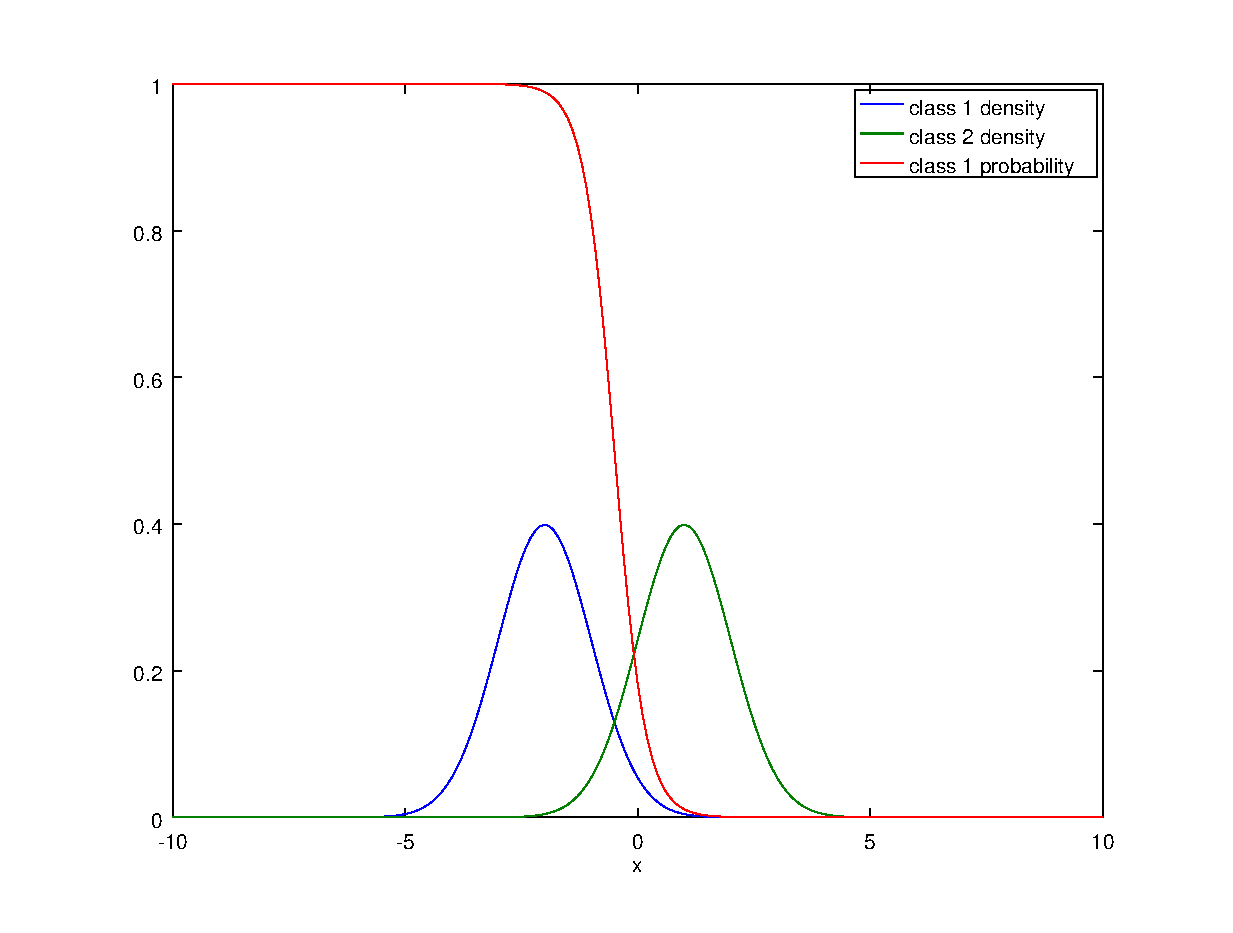
\includegraphics[width=0.5\textwidth]{../figures/equal-variance}Equal prior and variance}
      \only<3>{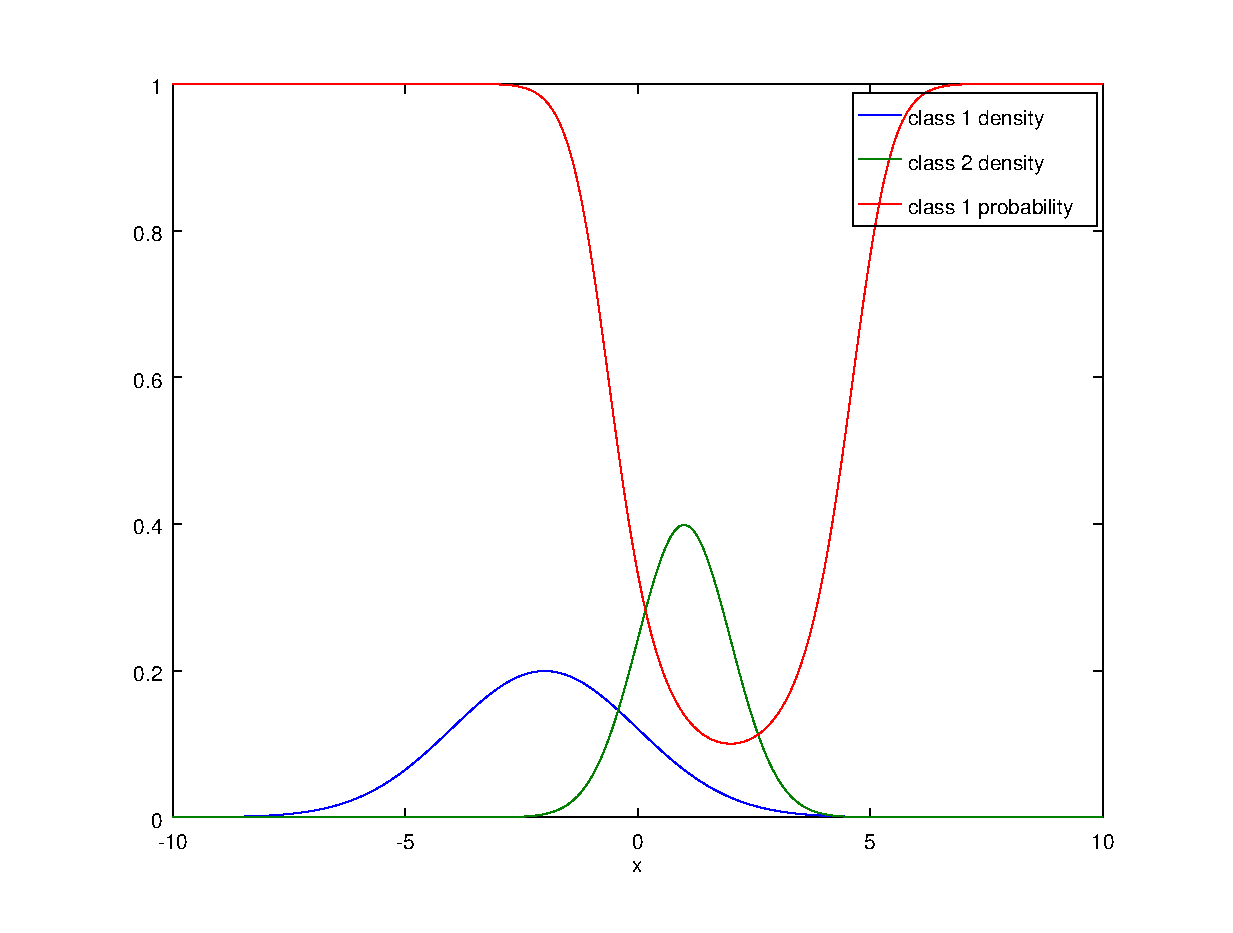
\includegraphics[width=0.5\textwidth]{../figures/unequal-variance}Unequal variance}
\only<5>{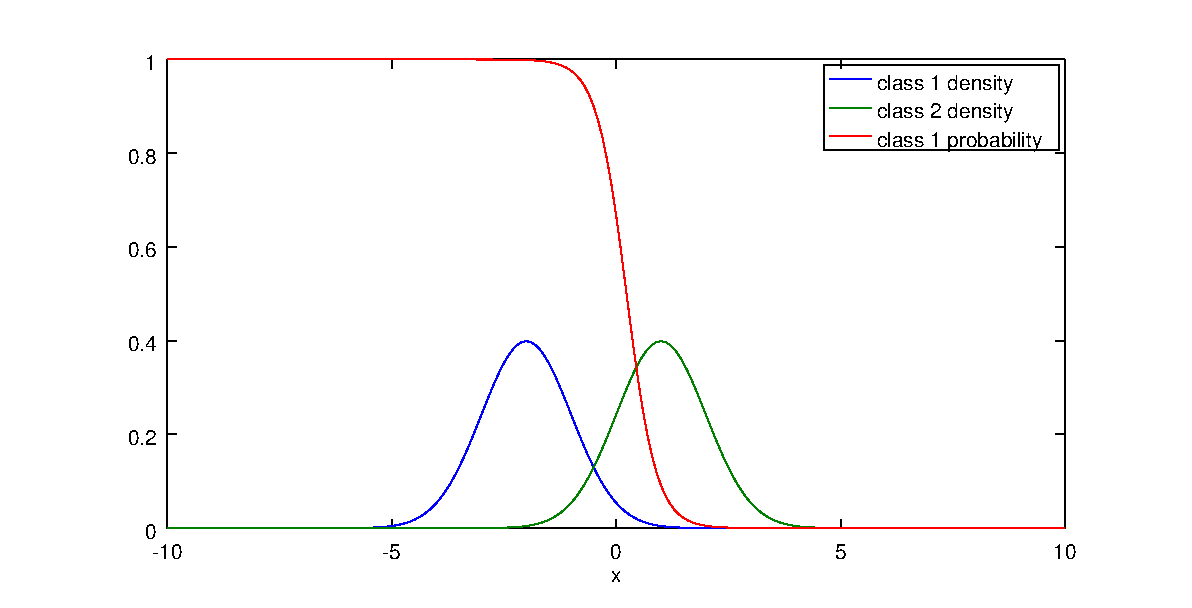
\includegraphics[width=0.5\textwidth]{../figures/unequal-prior}Unequal prior}
    \end{example}
  }
  \uncover<5>{
    \alert{But how can we get a probability model in the first place?}
  }
\end{frame}


  \begin{frame}
    \frametitle{Subjective probability}
    \only<article>{While probabilities apply to truly random events, they are also useful for representing subjective uncertainty. In this course, we will use a special symbol for subjective probability, $\bel$.}
    \begin{block}{Subjective probability measure $\bel$}
      \begin{itemize}
      \item If we think event $A$ is more likely than $B$, then $\bel(A) > \bel(B)$.
      \item Usual rules of probability apply:
        \begin{enumerate}
        \item $\bel(A) \in [0,1]$.
        \item $\bel(\emptyset) = 0$.
        \item If $A \cap B = \emptyset$, then $\bel(A \cup B) = \bel(A) + \bel(B)$.
        \end{enumerate}
      \end{itemize}
    \end{block}
  \end{frame}


  \begin{frame}
    \frametitle{Bayesian inference illustration}
    \begin{columns}
      \begin{column}{0.7\textwidth}
        \begin{block}{Use a subjective belief $\bel(\model)$ on $\Model$}
          \begin{itemize}
          \item<1-> \alert{Prior} belief $\bel(\model)$ represents our initial uncertainty.
          \item<2-> We \alert{observe history} $h$.
          \item<3->Each possible $\model$ assigns a \alert{probability} $P_\model(h)$ to $h$.
          \item<4-> We can use this to \alert{update} our belief via Bayes' theorem to obtain the \alert{posterior} belief:
            \[
            \bel(\model \mid h) \propto P_\model(h) \bel(\model)
            \tag{conclusion = evidence $\times$ prior}
            \]
          \end{itemize}
        \end{block}
      \end{column}
      \begin{column}{0.3\textwidth}
        \centering
\uncover<1->{\includegraphics[width=0.5\fwidth]{../figures/rl_worlds}
          \\
          prior
        }
        \\
        \uncover<2->{\includegraphics[width=0.5\fwidth]{../figures/rl_observations}
          \\
          evidence
        }
        \\
        \uncover<4->{\includegraphics[width=0.5\fwidth]{../figures/rl_worlds2}
          \\ 
          conclusion
        }
      \end{column}
    \end{columns}
  \end{frame}




  \subsection{Probability and Bayesian inference}
  \only<article>{One of the most important methods in machine learning
    and statistics is that of Bayesian inference.  This is the most
    fundamental method of drawing conclusions from data and explicit
    prior assumptions. In Bayesian inference, prior assumptions are
    represented as a probabilities on a space of hypotheses. Each
    hypothesis is seen as a probabilistic model of all possible data
    that we can see.}

  \only<article>{Frequently, we want to draw conclusions from data. However, the conclusions are never solely inferred from data, but also depend on prior assumptions about reality.}




  \begin{frame}
    \frametitle{Some examples}

    \begin{example}
      John claims to be a medium. He throws a coin $n$ times and predicts its value always correctly. Should we believe that he is a medium?
      \begin{itemize}
      \item $\model_1$: John is a medium.
      \item $\model_0$: John is not a medium.
      \end{itemize}
    \end{example}
    The answer depends on what we \alert{expect} a medium to be able to do, and how likely we thought he'd be a medium in the first place.

    \only<article>{
    \begin{example}
      Traces of DNA are found at a murder scene. We perform a DNA test against a database of $10^4$ citizens registered to be living in the area. We know that the probability of a false positive (that is, the test finding a match by mistake) is $10^{-6}$. If there is a match in the database, does that mean that the citizen was at the scene of the crime?
    \end{example}
    }
  \end{frame}





  \begin{frame}
    \frametitle{Bayesian inference}
    \only<article>{
      Now let us apply this idea to our specific problem. We already have the probability of the observation for each model, but we just need to define a \emph{prior probability} for each model. Since this is usually completely subjective, we give it another symbol.
    }
    \only<article>{
      \begin{block}{Prior probability}
        The prior probability $\bel$ on a set of models $\Model$ specifies our subjective belief $\bel(\model)$ that each model is true.\footnote{More generally $\bel$ is a probability measure.}
      \end{block}
    }
    \only<article>{
      This allows us to calculate the probability of John being a medium, given the data:
      \[
      \bel(\model_1 \mid \bx) = \frac{\Pr(\bx \mid \model_1) \bel(\model_1)}{\Pr_\bel(\bx)},
      \]
      where
      \[
      \Pr_\bel(\bx) \defn \Pr(\bx \mid \model_1) \bel(\model_1) + \Pr(\bx \mid \model_0) \bel(\model_0).
      \]
      The only thing left to specify is $\bel(\model_1)$, the probability that John is a medium before seeing the data. This is our subjective prior belief that mediums exist and that John is one of them.
      More generally, we can think of Bayesian inference as follows: }
    \begin{itemize}
    \item<1-> \only<article>{We start with a set of } mutually exclusive models $\Model = \{\model_1, \ldots, \model_k\}$.
    \item<2->\only<article>{Each model $\model$ is represented by a specific probabilistic model for any possible data $x$, that is}
      \only<presentation>{Probability model for any data $x$:} $P_\model(x) \equiv \Pr(x \mid \model)$.
    \item<3-> For each model, we have a prior probability $\bel(\model)$ that it is correct.
    \item<4-> \only<article>{After observing the data, we can calculate a posterior probability that the model is correct:}
      \only<presentation>{Posterior probability}
      \[
      \bel(\model \mid x) = \frac{\Pr(x \mid \model) \bel(\model)}{\sum_{\model' \in \Model} \Pr(x \mid \model') \bel(\model')}
      = \frac{P_\model(x) \bel(\model)}{\sum_{\model' \in \Model} P_{\model'} (x) \bel(\model')}.
      \]
    \end{itemize}
    \only<5->{
      \begin{block}{Interpretation}
        \begin{itemize}
        \item $\CM$: Set of all possible models that could describe the data.
        \item $P_\model(x)$: Probability of $x$ under model $\model$.
        \item Alternative notation $\Pr(x \mid \model)$: Probability of $x$ given that model $\model$ is correct.
        \item $\bel(\model)$: Our belief, before seeing the data, that $\model$ is correct.
        \item $\bel(\model \mid x)$: Our belief, aftering seeing the data, that $\model$ is correct.
      \end{itemize}
    \end{block}
    \only<article>{It must be emphasized that $P_\model(x) = \Pr(x \mid \model)$ as they are simply two different notations for the same thing. In words the first can be seen as the probability that model $\model$ assigns to data $x$, while the second as the probability of $x$ if $\model$ is the true model.}
  }
    \only<article>{
      Combining the prior belief with evidence is key in this procedure. Our posterior belief can then be used as a new prior belief when we get more evidence.}
  \end{frame}
\begin{frame}
\begin{exercise}[Continued example for medium]
    \only<article>{ Now let us apply this idea to our specific
      problem. We first make an independence assumption. In particular, we can assume that success and failure comes from a Bernoulli distribution with a parameter depending on the model.}
    \begin{align}
    P_{\model} (x) &= \prod_{t=1}^n P_{\model} (x_t).
\tag{independence property}
    \end{align}
    \only<article>{We first need to specify how well a medium could predict. Let's assume that a true medium would be able to predict perfectly, and that a non-medium would only predict randomly. This leads to the following models:}
    \begin{align}
      P_{\model_1}(x_t = 1) &= 1, &P_{\model_1}(x_t = 0) &= 0.
                                                           \tag{true medium model}
                                                           \\
      P_{\model_0}(x_t = 1) &= 1/2, &P_{\model_0}(x_t = 0) &= 1/2.
                                                             \tag{non-medium model}
    \end{align}
    \only<article>{
      The only thing left to specify is $\bel(\model_1)$, the probability
      that John is a medium before seeing the data. This is our
      subjective prior belief that mediums exist and that John is one of
      them.}
    \uncover<3->{
      \begin{align}
        \bel(\model_0) &= 1/2,   &  \bel(\model_1) &= 1/2.
                                                     \tag{prior belief}
      \end{align}
    }
    \only<article>{Combining the prior belief with evidence is key in this
      procedure. Our posterior belief can then be used as a new prior
      belief when we get more evidence.  }
    \uncover<4>{
      \begin{align}
      \bel(\model_1 \mid x) & = \frac{P_{\model_1}(x)
        \bel(\model_1)}{\Pr_\bel(x)} \tag{posterior belief}
        \\
      \Pr_\bel(x) &\defn P_{\model_1}(x) \bel(\model_1) + P_{\model_0}(x) \bel(\model_0).
\tag{marginal distribution}
      \end{align}
    }
    Throw a coin 4 times, and have a classmate make a prediction. What your belief that your classmate is a medium? Is the prior you used reasonable?
  \end{exercise}
  \end{frame}


\begin{frame}
  \frametitle{Sequential update of beliefs}
    \only<article>{Assume you have $n$ meteorologists. At each day $t$, each meteorologist $i$ gives a probability $p_{t,\model_i}\defn P_{\model_i}(x_t = \textrm{rain})$ for rain. Consider the case of there being three meteorologists, and each one making the following prediction for the coming week. Start with a uniform prior $\bel(\model) = 1/3$ for each model.}
    {
      \begin{table}[h]
        \begin{tabular}{c|l|l|l|l|l|l|l}
          &M&T&W&T&F&S&S\\
          \hline
          CNN & 0.5 & 0.6 & 0.7 & 0.9 & 0.5 & 0.3 & 0.1\\
          SMHI & 0.3 & 0.7 & 0.8 & 0.9 & 0.5 & 0.2 & 0.1\\
          YR & 0.6 & 0.9 & 0.8 & 0.5 & 0.4 & 0.1 & 0.1\\
          \hline
          Rain? & Y & Y & Y & N & Y & N & N
        \end{tabular}
        \caption{Predictions by three different entities for the probability of rain on a particular day, along with whether or not it actually rained.}
        \label{tab:meteorologists}
      \end{table}
    }
  \begin{exercise}
    \begin{itemize}
    \item $n$ meteorological stations $\cset{\mdp_i}{i=1, \ldots,n}$
    \item The $i$-th station predicts rain $P_{\mdp_i}(x_t \mid x_1, \ldots, x_{t-1})$.
    \item Let $\bel_t(\mdp)$ be our belief at time $t$.
      Derive the next-step belief
      $\bel_{t+1}(\mdp) \defn  \bel_t(\mdp | y_{t})$ in terms of the current belief $\bel_t$.
    \item Write a python function that computes this posterior
    \end{itemize}
  \end{exercise}
  \uncover<2->{
    \[
      \bel_{t+1}(\mdp)
      \defn
      \bel_t(\mdp | x_{t})
      =
      \frac{P_\mdp(x_t \mid x_1, \ldots, x_{t-1}) \bel_t(\mdp)}
      {\sum_{\mdp'} P_{\mdp'}(x_t \mid x_1, \ldots, x_{t-1}) \bel_t(\mdp')}
    \]
  }
\end{frame}



\begin{frame}[label=beta-example]
  \frametitle{Bayesian inference for Bernoulli distributions}
  \only<1>{
    \begin{block}{Estimating a coin's bias}
      A fair coin comes heads $50\%$ of the time. 
      We want to test an unknown coin, which we think may not be completely fair. 
    \end{block}
  }
  \only<1,2>{
    \begin{figure}[h]
      \centering
      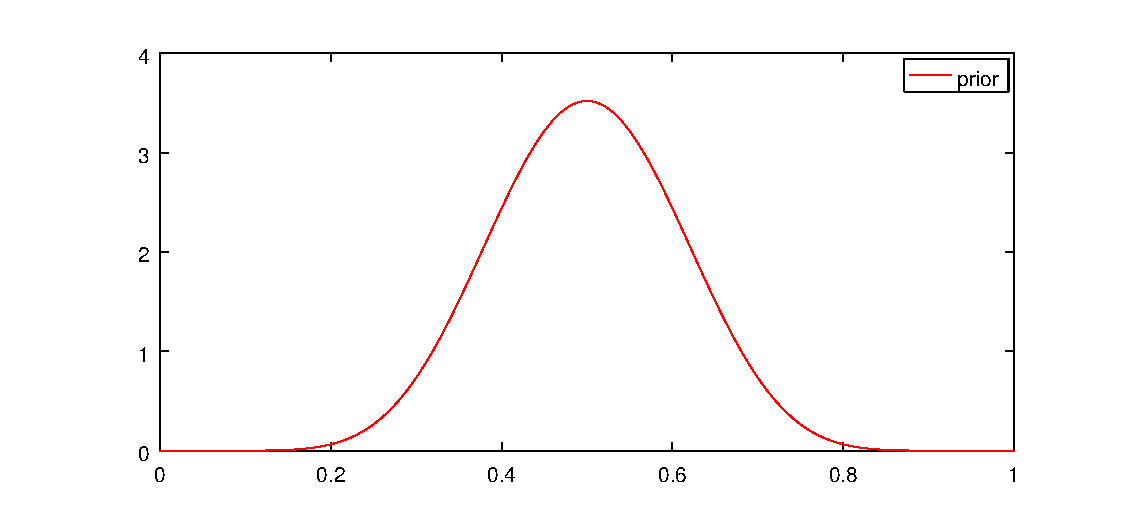
\includegraphics[width=\textwidth]{../figures/beta-prior}
      \caption{Prior belief $\bel$ about the coin bias $\theta$.}
    \end{figure}
  }
  \only<2>{
    For a sequence of throws $x_t \in \{0,1\}$,
    \[
    P_\theta(x) \propto \prod_t \theta^{x_t} (1 - \theta)^{1 - x_t}
    = \theta^{\textrm{\#Heads}} (1 - \theta)^{\textrm{\#Tails}}
    \]
  }
  \only<3>{
    \begin{figure}[h]
      \centering
      \includegraphics[width=\textwidth]{../figures/beta-likelihood}
      \caption{Prior belief $\bel$ about the coin bias $\theta$ and likelihood of $\theta$ for the data.}
    \end{figure}
    Say we throw the coin 100 times and obtain 70 heads. Then we plot the \alert{likelihood} $P_\theta(x)$ of different models.
  }
  \only<4>{
    \begin{figure}[h]
      \centering
      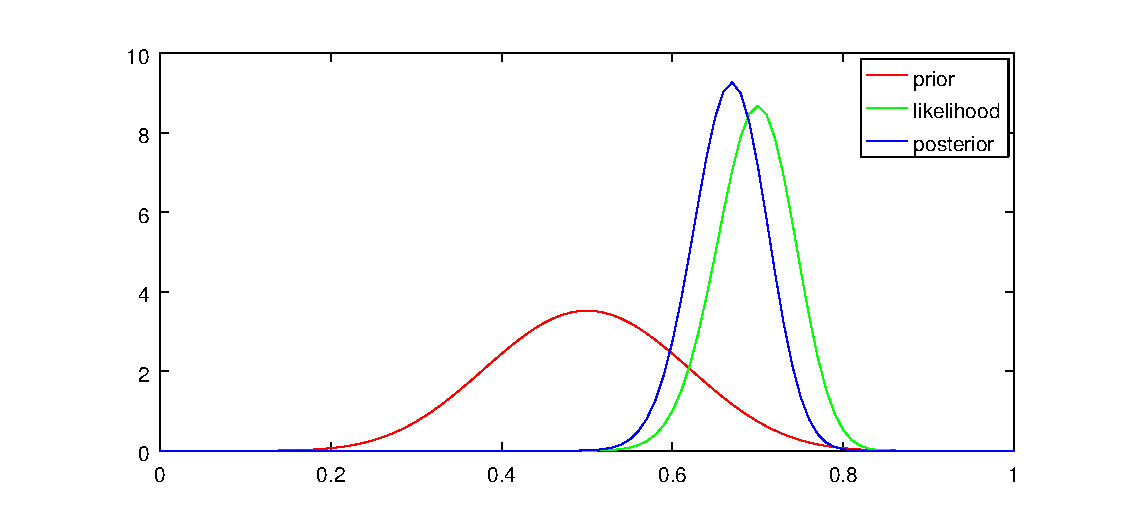
\includegraphics[width=\textwidth]{../figures/beta-posterior}
      \caption{Prior belief $\bel(\theta)$ about the coin bias $\theta$, likelihood of $\theta$ for the data, and posterior belief $\bel(\theta \mid x)$}
    \end{figure}
    From these, we calculate a \alert{posterior} distribution over the correct models. This represents our conclusion given our prior and the data.
  }
  \only<article>{If the prior distribution is described by the so-called Beta density
    \[
    f(\theta \mid \alpha, \beta) \propto \theta^{\alpha -1} (1 - \theta)^{\beta -1}
    \]
    where $\alpha, \beta$ describe the shape of the Beta distribution.
  }
\end{frame}



\begin{frame}
  \frametitle{Learning outcomes}
  \begin{block}{Understanding}
    \begin{itemize}
    \item The axioms of probability, marginals and conditional distributions.
    \item The philosophical underpinnings of Bayesianism.
    \item The simple conjugate model for Bernoulli distributions.
    \end{itemize}
  \end{block}
  
  \begin{block}{Skills}
    \begin{itemize}
    \item Be able to calculate with probabilities using the marginal and conditional definitions and Bayes rule.
    \item Being able to implement a simple Bayesian inference algorithm in Python.
    \end{itemize}
  \end{block}

  \begin{block}{Reflection}
    \begin{itemize}
    \item How useful is the Bayesian representation of uncertainty?
    \item How restrictive is the need to select a prior distribution?
    \item Can you think of another way to explicitly represent uncertainty in a way that can incorporate new evidence?
    \end{itemize}
  \end{block}
  
\end{frame}

  %%% Local Variables:
  %%% mode: latex
  %%% TeX-engine: xetex
  %%% TeX-master: "notes.tex"
  %%% End:
 % Bayesian inference
\section{Hierarchies of decision making problems}
\label{sec:decision-problems}
\only<presentation>{
  \begin{frame}
    \tableofcontents[ 
    currentsection, 
    hideothersubsections, 
    sectionstyle=show/shaded
    ] 
  \end{frame}
}


\only<article>{
  All machine learning problems are essentially decision problems. This essentially means replacing some human decisions with machine decisions. One of the simplest decision problems is classification, where you want an algorithm to decide the correct class of some data, but even within this simple framework there is a multitude of decisions to be made. The first is how to frame the classification problem the first place. The second is how to collect, process and annotate the data. The third is choosing the type of classification model to use. The fourth is how to use the collected data to find an optimal classifier within the selected type. After all this has been done, there is the problem of classifying new data. In this course, we will take a holistic view of the problem, and consider each problem in turn, starting from the lowest level and working our way up.}


\subsection{Simple decision problems}
\begin{frame}
  \frametitle{Preferences}
  \only<article>{The simplest decision problem involves selecting one item from a set of choices, such as in the following examples}  
  \begin{example}
    \begin{block}{Food}
      \begin{itemize}
      \item[A] McDonald's cheeseburger
      \item[B] Surstromming
      \item[C] Oatmeal
      \end{itemize}
    \end{block}
    \begin{block}{Money}
      \begin{itemize}
      \item[A] 10,000,000 SEK
      \item[B] 10,000,000 USD
      \item[C] 10,000,000 BTC
      \end{itemize}
    \end{block}
    \begin{block}{Entertainment}
      \begin{itemize}
      \item[A] Ticket to Liseberg
      \item[B] Ticket to Rebstar
      \item[C] Ticket to Nutcracker
      \end{itemize}
    \end{block}
  \end{example}
\end{frame}

\begin{frame}
  \frametitle{Rewards and utilities}
  \only<article>{In the decision theoretic framework, the things we receive are called rewards, and we assign a utility value to each one of them, showing which one we prefer.}
  \begin{itemize}
  \item Each choice is called a \alert{reward} $r \in \CR$.
  \item There is a \alert{utility function} $U : \CR \to \Reals$, assigning values to reward.
  \item We (weakly) prefer $A$ to $B$ iff $U(A) \geq U(B)$.
  \end{itemize}
  \only<article>{In each case, given $U$ the choice between each reward is trivial. We just select the reward:
    \[
    r^* \in \argmax_r U(r)
    \]
    The main difficult is actually selecting the appropriate utility function. In a behavioural context, we simply assume that humans act with respect to a specific utility function. However, figuring out this function from behavioural data is non trivial. ven when this assumption is correct, individuals do not have a common utility function.
  }
  \begin{exercise}
    From your individual preferences, derive a \alert{common utility function} that reflects everybody's preferences in the class for each of the three examples. Is there a simple algorithm for deciding this? Would you consider the outcome fair?
  \end{exercise}
\end{frame}

\begin{frame}
  \frametitle{Preferences among random outcomes}
  \begin{example}
    Would you rather \ldots
    \begin{itemize}
    \item[A] Have 100 EUR now?
    \item[B] Flip a coin, and get 200 EUR if it comes heads?
    \end{itemize}    
  \end{example}
  \uncover<2->{
    \begin{block}{The expected utility hypothesis}
      Rational decision makers prefer choice $A$ to $B$ if
      \[
      \E(U | A) \geq \E(U | B),
      \]
      where the expected utility is
      \[
      \E(U | A) = \sum_r U(r) \Pr(r | A).
      \]
    \end{block}
    In the above example, $r \in \{0, 100, 200\}$ and $U(r)$ is
    increasing, and the coin is fair.
  }
  \begin{block}{Risk\index{risk} and monetary rewards}
    \only<article>{When $r \in \Reals$, as in the case of monetary rewards, we can use the shape of the utility function determines the amount of risk aversion. In particular:}
    \begin{itemize}
    \item<3-> If $U$ is convex, we are risk-seeking. \only<article>{In the example above, we would prefer B to A, as the expected utility of B would be higher than A, even though they give the same amount of money on average.}
    \item<4-> If $U$ is linear, we are risk neutral. \only<article>{In the example above, we would be indifferent between $A$ and $B$, as the expected amount of money is the same as the amount of money we get.}
    \item<5-> If $U$ is concave, we are risk-averse. \only<article>{Hence, in the example above, we prefer A.}
    \end{itemize}
  \end{block}
  \only<article>{This idea of risk can be used with any other utility function. We can simply replace the original utility function $U$ with a monotonic function $f(U)$ to achieve risk-sensitive behaviour. However, this is not the only risk-sensitive approach possible.}
\end{frame}


\begin{frame}
  \frametitle{Uncertain rewards}
  \only<article>{However, in real life, there are many cases where we can only choose between uncertain outcomes. The simplest example are lottery tickets, where rewards are essentially random. However, in many cases the rewards are not really random, but simply uncertain. In those cases it is useful to represent our uncertainty with probabilities as well, even though there is nothing really random.}
  \begin{itemize}
  \item Decisions $\decision \in \Decision$
  \item Each choice is called a \alert{reward} $r \in \CR$.
  \item There is a \alert{utility function} $U : \CR \to \Reals$, assigning values to reward.
  \item We (weakly) prefer $A$ to $B$ iff $U(A) \geq U(B)$.
  \end{itemize}

  \begin{example}
    \begin{columns}
      \begin{column}{0.5\textwidth}
        You are going to work, and it might rain.  What do you do?
        \begin{itemize}
        \item $\decision_1$: Take the umbrella.
        \item $\decision_2$: Risk it!
        \item $\outcome_1$: rain
        \item $\outcome_2$: dry
        \end{itemize}
      \end{column}
      \begin{column}{0.5\textwidth}
        \begin{table}
          \centering
          \begin{tabular}{c|c|c}
            $\Rew(\outcome,\decision)$ & $\decision_1$ & $\decision_2$ \\ %ro: U has only one argument.
            \hline
            $\outcome_1$ & dry, carrying umbrella & wet\\
            $\outcome_2$ & dry, carrying umbrella & dry\\
            \hline
            \hline
            $U[\Rew(\outcome,\decision)]$ & $\decision_1$ & $\decision_2$ \\
            \hline
            $\outcome_1$ & 0 & -10\\
            $\outcome_2$ & 0 & 1
          \end{tabular}
          \caption{Rewards and utilities.}
          \label{tab:rain-utility-function}
        \end{table}

        \begin{itemize}
        \item<2-> $\max_\decision \min_\outcome U = 0$
        \item<3-> $\min_\outcome \max_\decision U = 0$
        \end{itemize}
      \end{column}

    \end{columns}
  \end{example}
\end{frame}



\begin{frame}
  \frametitle{Expected utility}
  \[
  \E (U \mid a) = \sum_r U[\Rew(\outcome, \decision)] \Pr(\outcome \mid \decision)
  \]
  \begin{example}%ro: rather an exercise?
    You are going to work, and it might rain. The forecast said that
    the probability of rain $(\outcome_1)$ was $20\%$. What do you do?
    \begin{itemize}
    \item $\decision_1$: Take the umbrella.
    \item $\decision_2$: Risk it!
    \end{itemize}
    \begin{table}
      \centering
      \begin{tabular}{c|c|c}
        $\Rew(\outcome,\decision)$ & $\decision_1$ & $\decision_2$ \\ %ro: U has only one argument.
        \hline
        $\outcome_1$ & dry, carrying umbrella & wet\\
        $\outcome_2$ & dry, carrying umbrella & dry\\
        \hline
        \hline
        $U[\Rew(\outcome,\decision)]$ & $\decision_1$ & $\decision_2$ \\
        \hline
        $\outcome_1$ & 0 & -10\\
        $\outcome_2$ & 0 & 1\\
        \hline
        \hline
        $\E(U \mid \decision)$ & 0 &  -1.2 \\ 
      \end{tabular}
      \caption{Rewards, utilities, expected utility for $20\%$ probability of rain.}
      \label{tab:rain-utility-function}
    \end{table}
  \end{example}
\end{frame}





\subsection{Decision rules}

\only<article>{We now move from simple decisions to decisions that
  depend on some observation. We shall start with a simple problem in applied meteorology. Then we will discuss hypothesis testing as a decision making problem. Finally, we will go through an exercise in Bayesian methods for classification.}

\begin{frame}
  \frametitle{Bayes decision rules}
  Consider the case where outcomes are independent of decisions:
  \[
  \util (\bel, \decision) \defn \sum_{\model}  \util (\model, \decision) \bel(\model)
  \]
  This corresponds e.g. to the case where $\bel(\model)$ is the belief about an unknown world.
  \begin{definition}[Bayes utility]
    \label{def:bayes-utility}
    The maximising decision for $\bel$ has an expected utility equal to:
    \begin{equation}
      \BUtil(\bel) \defn \max_{\decision \in \Decision} \util (\bel, \decision).
      \label{eq:bayes-utility}
    \end{equation}
  \end{definition}
\end{frame}




\begin{frame}
  \frametitle{The $n$-meteorologists problem}
  \index{$n$-meteorologists|textbf}
  \only<article>{Of course, we may not always just be interested in classification performance in terms of predicting the most likely class. It strongly depends on the problem we are actually wanting to solve. In  biometric authentication, for example, we want to guard against the unlikely event that an impostor will successfully be authenticated. Even if the decision rule that always says 'OK' has the lowest classification error in practice, the expected cost of impostors means that the optimal decision rule must sometimes say 'Failed' even if this leads to false rejections sometimes.}
  \begin{exercise}
    \only<presentation>{
      \only<1>{
        \begin{itemize}
        \item Meteorological models $\CM = \set{\model_1, \ldots, \model_n}$
        \item Rain predictions at time $t$: $p_{t,\model} \defn  P_{\model}(x_t = \textrm{rain})$.
        \item Prior probability $\bel(\model) = 1/n$ for each model.
        \item Should we take the umbrella?
        \end{itemize}
      }
    }
    \only<article>{Assume you have $n$ meteorologists. At each day $t$, each meteorologist $i$ gives a probability $p_{t,\model_i}\defn P_{\model_i}(x_t = \textrm{rain})$ for rain. Consider the case of there being three meteorologists, and each one making the following prediction for the coming week. Start with a uniform prior $\bel(\model) = 1/3$ for each model.}
    {
      \begin{table}[h]
        \begin{tabular}{c|l|l|l|l|l|l|l}
          &M&T&W&T&F&S&S\\
          \hline
          CNN & 0.5 & 0.6 & 0.7 & 0.9 & 0.5 & 0.3 & 0.1\\
          SMHI & 0.3 & 0.7 & 0.8 & 0.9 & 0.5 & 0.2 & 0.1\\
          YR & 0.6 & 0.9 & 0.8 & 0.5 & 0.4 & 0.1 & 0.1\\
          \hline
          Rain? & Y & Y & Y & N & Y & N & N
        \end{tabular}
        \caption{Predictions by three different entities for the probability of rain on a particular day, along with whether or not it actually rained.}
        \label{tab:meteorologists}
      \end{table}
    }
    \uncover<2->{
      \begin{enumerate}
      \item<2-> What is your belief about the quality of each meteorologist after each day? 
      \item<3-> What is your belief about the probability of rain each day? 
        \[
        P_\bel(x_t = \textrm{rain} \mid x_1, x_2, \ldots x_{t-1})
        =
        \sum_{\model \in \Model} P_\model(x_t = \textrm{rain} \mid x_1, x_2, \ldots x_{t-1})
        \bel(\model \mid x_1, x_2, \ldots x_{t-1}) 
        \]
      \item<4-> Assume you can decide whether or not to go running each
        day. If you go running and it does not rain, your utility is 1. If
        it rains, it's -10. If you don't go running, your utility is
        0. What is the decision maximising utility in expectation (with respect to the posterior) each
        day?
      \end{enumerate}
    }
    \label{ex:meteorologists}
  \end{exercise}
\end{frame}


\only<article>{
  \subsection{Statistical testing\textsuperscript{*}}
\only<article>{A common type of decision problem is a statistical test. This arises when we have a set of possible candidate models $\CM$ and we need to be able to decide which model to select after we see the evidence.
  Many times, there is only one model under consideration, $\model_0$, the so-called \alert{null hypothesis}. Then, our only decision is whether or not to accept or reject this hypothesis.}
\begin{frame}
  \frametitle{Simple hypothesis testing}
  \only<article>{Let us start with the simple case of needing to compare two models.}
  \begin{block}{The simple hypothesis test as a decision problem}
    \begin{itemize}
    \item $\CM = \{\model_0, \model_1\}$
    \item $a_0$: Accept model $\model_0$
    \item $a_1$: Accept model $\model_1$
    \end{itemize}
    \begin{table}[H]
      \begin{tabular}{c|cc}
        $\util$& $\model_0$& $\model_1$\\\hline
        $a_0$ & 1 & 0\\
        $a_1$ & 0 & 1
      \end{tabular}
      \caption{Example utility function for simple hypothesis tests.}
    \end{table}
    \only<article>{There is no reason for us to be restricted to this utility function. As it is diagonal, it effectively treats both types of errors in the same way.}
  \end{block}

  \begin{example}[Continuation of the medium example]
    \begin{itemize}
    \item $\model_1$: that John is a medium.
    \item $\model_0$: that John is not a medium.
    \end{itemize}
    \only<article>{
      Let $x_t$ be $0$ if John makes an incorrect prediction at time $t$ and $x_t = 1$ if he makes a correct prediction. Let us once more assume a Bernoulli model, so that John's claim that he can predict our tosses perfectly means that for a sequence of tosses $\bx = x_1, \ldots, x_n$,
      \[
        P_{\model_1}(\bx) = \begin{cases}
          1, & x_t = 1 \forall t \in [n]\\
          0, & \exists t \in [n] : x_t = 0.
        \end{cases}
      \]
      That is, the probability of perfectly correct predictions is 1, and that of one or more incorrect prediction is 0. For the other model, we can assume that all draws are independently and identically distributed from a fair coin. Consequently, no matter what John's predictions are, we have that:
      \[
        P_{\model_0}(\bx = 1 \ldots 1) = 2^{-n}.
      \]
      So, for the given example, as stated, we have the following facts:
      \begin{itemize}
      \item If John makes one or more mistakes, then $\Pr(\bx \mid \model_1) = 0$ and $\Pr(\bx \mid \model_0) = 2^{-n}$. Thus, we should perhaps say that then John is not a medium
      \item If John makes no mistakes at all, then 
        \begin{align}
          \Pr(\bx = 1, \ldots, 1 \mid \model_1) &= 1,
          &
            \Pr(\bx = 1, \ldots, 1 \mid \model_0) &= 2^{-n}.
        \end{align}
      \end{itemize}
      Now we can calculate the posterior distribution, which is
      \[
        \bel(\model_1 \mid \bx = 1, \ldots, 1) = \frac{1 \times \bel(\model_1)}{1 \times \bel(\model_1) + 2^{-n} (1 - \bel(\model_1))}.
      \]
      Our expected utility for taking action $a_0$ is actually
    }
    \[
      \E_\bel(\util \mid a_0) = 1 \times \bel(\model_0 \mid \bx) + 0 \times \bel(\model_1 \mid \bx), \qquad
      \E_\bel(\util \mid a_1) = 0 \times \bel(\model_0 \mid \bx) + 1 \times \bel(\model_1 \mid \bx)
    \]
  \end{example}
  
\end{frame}


\begin{frame}
  \frametitle{Null hypothesis test}
    \index{Null-Hypothesis test}
  Many times, there is only one model under consideration, $\model_0$, the so-called \alert{null hypothesis}. \only<article>{ This happens when, for example, we have no simple way of defining an appropriate alternative. Consider the example of the medium: How should we expect a medium to predict? Then, our only decision is whether or not to accept or reject this hypothesis.}
  \begin{block}{The null hypothesis test as a decision problem}
    \begin{itemize}
    \item $a_0$: Accept model $\model_0$
    \item $a_1$: Reject model $\model_0$
    \end{itemize}
  \end{block}

  \begin{example}{Construction of the test for the medium}
    \index{policy!for statistical testing}
    \begin{itemize}
    \item<2-> $\model_0$ is simply the $\Bernoulli(1/2)$ model: responses are by chance.
    \item<3-> We need to design a policy $\pol(a \mid \bx)$ that accepts or rejects depending on the data.
    \item<4-> Since there is no alternative model, we can only construct this policy according to its properties when $\model_0$ is true.
    \item<5-> In particular, we can fix a policy that only chooses $a_1$ when $\model_0$ is true a proportion $\delta$ of the time.
    \item<6-> This can be done by construcing a threshold test from the inverse-CDF.
    \end{itemize}
  \end{example}
\end{frame}
\begin{frame}
  \frametitle{Using $p$-values to construct statistical tests}
  \begin{definition}[Null statistical test]
    \only<article>{
      A statistical test $\pol$ is a decision rule for accepting or rejecting a hypothesis on the basis of evidence. A $p$-value test rejects a hypothesis whenever the value of the statistic $f(x)$ is smaller than a threshold.}
    The statistic $f : \CX \to [0,1]$ is  designed to have the property:
    \[
      P_{\model_0}(\cset{x}{f(x) \leq \delta}) = \delta.
    \]
    If our decision rule is:
    \[
      \pol(a \mid x) =
      \begin{cases}
        a_0, & f(x) \geq \delta\\
        a_1, & f(x) < \delta,
      \end{cases}
    \]
    the probability of rejecting the null hypothesis when it is true is exactly $\delta$.
  \end{definition}
  \only<presentation>{The value of the statistic $f(x)$, otherwise known as the \alert{$p$-value}, is uninformative.}
  \only<article>{This is because, by definition, $f(x)$ has a uniform distribution under $\model_0$. Hence the value of $f(x)$ itself is uninformative: high and low values are equally likely. In theory we should simply choose $\delta$ before seeing the data and just accept or reject based on whether $f(x) \leq \delta$. However nobody does that in practice, meaning that $p$-values are used incorrectly. Better not to use them at all, if uncertain about their meaning.}
\end{frame}
\begin{frame}
  \begin{block}{Issues with $p$-values}
    \begin{itemize}
    \item They only measure quality of fit \alert{on the data}.
    \item Not robust to model misspecification. \only<article>{For example, zero-mean testing using the $\chi^2$-test has a normality assumption.}
    \item They ignore effect sizes. \only<article>{For example, a linear analysis may determine that there is a significant deviation from zero-mean, but with only a small effect size of 0.01. Thus, reporting only the $p$-value is misleading}
    \item They do not consider prior information. 
    \item They do not represent the probability of having made an error. \only<article>{In particular, a $p$-value of $\delta$ does not mean that the probability that the null hypothesis is false given the data $x$, is $\delta$, i.e. $\delta \neq \Pr(\neg \model_0 \mid x)$.}
    \item The null-rejection error probability is the same irrespective of the amount of data (by design).
    \end{itemize}
  \end{block}
\end{frame}

\begin{frame}
  \only<article>{Let us consider the example of the medium.}
  \begin{block}{$p$-values for the medium example}
    \begin{itemize}
    \item<2->$\model_0$ is simply the $\Bernoulli(1/2)$ model:
      responses are by chance. 
    \item<3->CDF: $P_{\model_0}(N \leq n \mid K = 100)$ \only<article> {is the probability of at most $N$ successes if we throw the coin 100 times. This is in fact the cumulative probability function of the binomial distribution. Recall that the binomial represents the distribution for the number of successes of independent experiments, each following a Bernoulli distribution.}
    \item<4->ICDF:  the number of successes that will happen with probability at least $\delta$
    \item<5->e.g. we'll get at most 50 successes a proportion $\delta = 1/2$ of the time.
    \item<6>Using the (inverse) CDF we can construct a policy $\pol$ that selects $a_1$ when $\model_0$ is true only a $\delta$ portion of the time, for any choice of $\delta$.
    \end{itemize}
  \end{block}
  \begin{columns}
    \setlength\fheight{0.33\columnwidth}
    \setlength\fwidth{0.33\columnwidth}
    \begin{column}{0.5\textwidth}
      \only<3,4,5,6>{% This file was created by matlab2tikz.
%
%The latest updates can be retrieved from
%  http://www.mathworks.com/matlabcentral/fileexchange/22022-matlab2tikz-matlab2tikz
%where you can also make suggestions and rate matlab2tikz.
%
\begin{tikzpicture}

\begin{axis}[%
width=\fwidth,
height=0.831\fheight,
at={(0\fwidth,0\fheight)},
scale only axis,
xmin=0,
xmax=100,
xlabel={Number of successes},
ymin=0,
ymax=1,
ylabel={Probability of less than N successes},
axis background/.style={fill=white}
]
\addplot [color=blue, forget plot]
  table[row sep=crcr]{%
0	7.8886090522101e-31\\
1	7.96749514273217e-29\\
2	3.98453643227134e-27\\
3	1.31543344806511e-25\\
4	3.2248444478818e-24\\
5	6.26162256269277e-23\\
6	1.0029797609618e-21\\
7	1.36307186640302e-20\\
8	1.60428183412199e-19\\
9	1.66102448972682e-18\\
10	1.53164508771899e-17\\
11	1.27042666774617e-16\\
12	9.5567876801385e-16\\
13	6.56490776101789e-15\\
14	4.14222593604009e-14\\
15	2.41271075196861e-13\\
16	1.30296790932804e-12\\
17	6.54899932503508e-12\\
18	3.07390330752401e-11\\
19	1.35138126102441e-10\\
20	5.57954452862595e-10\\
21	2.1686833167108e-09\\
22	7.9526642368932e-09\\
23	2.75679038792502e-08\\
24	9.05001310651458e-08\\
25	2.81814101710274e-07\\
26	8.33681324725063e-07\\
27	2.34620630632112e-06\\
28	6.28957500833936e-06\\
29	1.60800076478334e-05\\
30	3.92506982279687e-05\\
31	9.15716124411769e-05\\
32	0.000204388583713412\\
33	0.000436859918456193\\
34	0.000894965195743431\\
35	0.00175882086148508\\
36	0.00331856025796311\\
37	0.00601648786268185\\
38	0.0104893678389258\\
39	0.0176001001088524\\
40	0.0284439668204906\\
41	0.044313040057034\\
42	0.0666053096036057\\
43	0.0966739522478211\\
44	0.135626512036918\\
45	0.184100808663348\\
46	0.242059206803646\\
47	0.308649706794632\\
48	0.382176717201337\\
49	0.460205381306407\\
50	0.539794618693593\\
51	0.617823282798662\\
52	0.691350293205368\\
53	0.757940793196354\\
54	0.815899191336652\\
55	0.864373487963082\\
56	0.903326047752179\\
57	0.933394690396394\\
58	0.955686959942966\\
59	0.971556033179509\\
60	0.982399899891148\\
61	0.989510632161074\\
62	0.993983512137318\\
63	0.996681439742037\\
64	0.998241179138515\\
65	0.999105034804257\\
66	0.999563140081544\\
67	0.999795611416287\\
68	0.999908428387559\\
69	0.999960749301772\\
70	0.999983919992352\\
71	0.999993710424992\\
72	0.999997653793694\\
73	0.999999166318675\\
74	0.999999718185898\\
75	0.999999909499869\\
76	0.999999972432096\\
77	0.999999992047336\\
78	0.999999997831317\\
79	0.999999999442046\\
80	0.999999999864862\\
81	0.999999999969261\\
82	0.999999999993451\\
83	0.999999999998697\\
84	0.999999999999759\\
85	0.999999999999959\\
86	0.999999999999993\\
87	0.999999999999999\\
88	1\\
89	1\\
90	1\\
91	1\\
92	1\\
93	1\\
94	1\\
95	1\\
96	1\\
97	1\\
98	1\\
99	1\\
100	1\\
};
\end{axis}
\end{tikzpicture}%}      
    \end{column}
    \begin{column}{0.5\textwidth}
      \only<4,5,6>{% This file was created by matlab2tikz.
%
%The latest updates can be retrieved from
%  http://www.mathworks.com/matlabcentral/fileexchange/22022-matlab2tikz-matlab2tikz
%where you can also make suggestions and rate matlab2tikz.
%
\begin{tikzpicture}

\begin{axis}[%
width=\fwidth,
height=0.831\fheight,
at={(0\fwidth,0\fheight)},
scale only axis,
xmin=0,
xmax=1,
xlabel={Probability of less than N successes},
ymin=0,
ymax=100,
ylabel={Number of successes},
axis background/.style={fill=white}
]
\addplot [color=blue, forget plot]
  table[row sep=crcr]{%
0	0\\
0.01	38\\
0.02	40\\
0.03	41\\
0.04	41\\
0.05	42\\
0.06	42\\
0.07	43\\
0.08	43\\
0.09	43\\
0.1	44\\
0.11	44\\
0.12	44\\
0.13	44\\
0.14	45\\
0.15	45\\
0.16	45\\
0.17	45\\
0.18	45\\
0.19	46\\
0.2	46\\
0.21	46\\
0.22	46\\
0.23	46\\
0.24	46\\
0.25	47\\
0.26	47\\
0.27	47\\
0.28	47\\
0.29	47\\
0.3	47\\
0.31	48\\
0.32	48\\
0.33	48\\
0.34	48\\
0.35	48\\
0.36	48\\
0.37	48\\
0.38	48\\
0.39	49\\
0.4	49\\
0.41	49\\
0.42	49\\
0.43	49\\
0.44	49\\
0.45	49\\
0.46	49\\
0.47	50\\
0.48	50\\
0.49	50\\
0.5	50\\
0.51	50\\
0.52	50\\
0.53	50\\
0.54	51\\
0.55	51\\
0.56	51\\
0.57	51\\
0.58	51\\
0.59	51\\
0.6	51\\
0.61	51\\
0.62	52\\
0.63	52\\
0.64	52\\
0.65	52\\
0.66	52\\
0.67	52\\
0.68	52\\
0.69	52\\
0.7	53\\
0.71	53\\
0.72	53\\
0.73	53\\
0.74	53\\
0.75	53\\
0.76	54\\
0.77	54\\
0.78	54\\
0.79	54\\
0.8	54\\
0.81	54\\
0.82	55\\
0.83	55\\
0.84	55\\
0.85	55\\
0.86	55\\
0.87	56\\
0.88	56\\
0.89	56\\
0.9	56\\
0.91	57\\
0.92	57\\
0.93	57\\
0.94	58\\
0.95	58\\
0.96	59\\
0.97	59\\
0.98	60\\
0.99	62\\
1	86\\
};
\end{axis}
\end{tikzpicture}%}
    \end{column}
  \end{columns}    
\end{frame}



\begin{frame}
  \frametitle{Constructing a Null-Hypothesis test with frequentist properties}
  \index{Null-Hypothesis test!frequentist}
  \begin{block}{The test statistic}
    We want the test to reflect that we don't have a significant number of failures.
    \[
      f(x) = 1 - \textrm{binocdf}(\sum_{t=1}^n x_t, n, 0.5)
    \]
  \end{block}
  \begin{alertblock}{What $f(x)$ is and is not}
    \begin{itemize}
    \item It is a \textbf{statistic} which is $\leq \delta$ a $\delta$ portion of the time when $\model_0$ is true.
    \item It is \textbf{not} the probability of observing $x$ under $\model_0$.
    \item It is \textbf{not} the probability of $\model_0$ given $x$.
    \end{itemize}
  \end{alertblock}
\end{frame}
\begin{frame}
  \begin{exercise}
    \begin{itemize}
    \item<1-> Let us throw a coin 8 times, and try and predict the outcome.
    \item<2-> Select a $p$-value threshold so that $\delta = 0.05$. 
      For 8 throws, this corresponds to \uncover<3->{$ > 6$ successes or $\geq 87.5\%$ success rate}.
    \item<3-> Let's calculate the $p$-value for each one of you
    \item<4-> What is the rejection performance of the test?
    \end{itemize}
    \setlength\fheight{0.25\columnwidth}
    \setlength\fwidth{0.5\columnwidth}
    \only<2,3>{
      \begin{figure}[H]
        \centering
        % This file was created by matlab2tikz.
%
%The latest updates can be retrieved from
%  http://www.mathworks.com/matlabcentral/fileexchange/22022-matlab2tikz-matlab2tikz
%where you can also make suggestions and rate matlab2tikz.
%
\begin{tikzpicture}

\begin{axis}[%
width=0.951\fwidth,
height=\fheight,
at={(0\fwidth,0\fheight)},
scale only axis,
xmin=0,
xmax=1000,
ymin=0,
ymax=0.5,
axis background/.style={fill=white},
title={The rejection threshold as data increases}
]
\addplot [color=blue, forget plot]
  table[row sep=crcr]{%
1	0\\
2	0\\
3	0\\
4	0\\
5	0.2\\
6	0.166666666666667\\
7	0.142857142857143\\
8	0.25\\
9	0.222222222222222\\
10	0.2\\
11	0.272727272727273\\
12	0.25\\
13	0.307692307692308\\
14	0.285714285714286\\
15	0.266666666666667\\
16	0.3125\\
17	0.294117647058824\\
18	0.333333333333333\\
19	0.315789473684211\\
20	0.3\\
21	0.333333333333333\\
22	0.318181818181818\\
23	0.347826086956522\\
24	0.333333333333333\\
25	0.32\\
26	0.346153846153846\\
27	0.333333333333333\\
28	0.357142857142857\\
29	0.344827586206897\\
30	0.366666666666667\\
31	0.354838709677419\\
32	0.34375\\
33	0.363636363636364\\
34	0.352941176470588\\
35	0.371428571428571\\
36	0.361111111111111\\
37	0.378378378378378\\
38	0.368421052631579\\
39	0.358974358974359\\
40	0.375\\
41	0.365853658536585\\
42	0.380952380952381\\
43	0.372093023255814\\
44	0.386363636363636\\
45	0.377777777777778\\
46	0.369565217391304\\
47	0.382978723404255\\
48	0.375\\
49	0.387755102040816\\
50	0.38\\
51	0.392156862745098\\
52	0.384615384615385\\
53	0.39622641509434\\
54	0.388888888888889\\
55	0.381818181818182\\
56	0.392857142857143\\
57	0.385964912280702\\
58	0.396551724137931\\
59	0.389830508474576\\
60	0.4\\
61	0.39344262295082\\
62	0.403225806451613\\
63	0.396825396825397\\
64	0.390625\\
65	0.4\\
66	0.393939393939394\\
67	0.402985074626866\\
68	0.397058823529412\\
69	0.405797101449275\\
70	0.4\\
71	0.408450704225352\\
72	0.402777777777778\\
73	0.397260273972603\\
74	0.405405405405405\\
75	0.4\\
76	0.407894736842105\\
77	0.402597402597403\\
78	0.41025641025641\\
79	0.405063291139241\\
80	0.4125\\
81	0.407407407407407\\
82	0.414634146341463\\
83	0.409638554216867\\
84	0.404761904761905\\
85	0.411764705882353\\
86	0.406976744186047\\
87	0.413793103448276\\
88	0.409090909090909\\
89	0.415730337078652\\
90	0.411111111111111\\
91	0.417582417582418\\
92	0.41304347826087\\
93	0.419354838709677\\
94	0.414893617021277\\
95	0.410526315789474\\
96	0.416666666666667\\
97	0.412371134020619\\
98	0.418367346938776\\
99	0.414141414141414\\
100	0.42\\
101	0.415841584158416\\
102	0.42156862745098\\
103	0.41747572815534\\
104	0.423076923076923\\
105	0.419047619047619\\
106	0.424528301886792\\
107	0.420560747663551\\
108	0.416666666666667\\
109	0.422018348623853\\
110	0.418181818181818\\
111	0.423423423423423\\
112	0.419642857142857\\
113	0.424778761061947\\
114	0.421052631578947\\
115	0.426086956521739\\
116	0.422413793103448\\
117	0.427350427350427\\
118	0.423728813559322\\
119	0.428571428571429\\
120	0.425\\
121	0.421487603305785\\
122	0.426229508196721\\
123	0.422764227642276\\
124	0.42741935483871\\
125	0.424\\
126	0.428571428571429\\
127	0.425196850393701\\
128	0.4296875\\
129	0.426356589147287\\
130	0.430769230769231\\
131	0.427480916030534\\
132	0.431818181818182\\
133	0.428571428571429\\
134	0.425373134328358\\
135	0.42962962962963\\
136	0.426470588235294\\
137	0.430656934306569\\
138	0.427536231884058\\
139	0.431654676258993\\
140	0.428571428571429\\
141	0.432624113475177\\
142	0.429577464788732\\
143	0.433566433566434\\
144	0.430555555555556\\
145	0.43448275862069\\
146	0.431506849315068\\
147	0.435374149659864\\
148	0.432432432432432\\
149	0.429530201342282\\
150	0.433333333333333\\
151	0.43046357615894\\
152	0.434210526315789\\
153	0.431372549019608\\
154	0.435064935064935\\
155	0.432258064516129\\
156	0.435897435897436\\
157	0.43312101910828\\
158	0.436708860759494\\
159	0.433962264150943\\
160	0.4375\\
161	0.434782608695652\\
162	0.438271604938272\\
163	0.43558282208589\\
164	0.432926829268293\\
165	0.436363636363636\\
166	0.433734939759036\\
167	0.437125748502994\\
168	0.43452380952381\\
169	0.437869822485207\\
170	0.435294117647059\\
171	0.43859649122807\\
172	0.436046511627907\\
173	0.439306358381503\\
174	0.436781609195402\\
175	0.44\\
176	0.4375\\
177	0.440677966101695\\
178	0.438202247191011\\
179	0.441340782122905\\
180	0.438888888888889\\
181	0.43646408839779\\
182	0.43956043956044\\
183	0.437158469945355\\
184	0.440217391304348\\
185	0.437837837837838\\
186	0.440860215053763\\
187	0.438502673796791\\
188	0.441489361702128\\
189	0.439153439153439\\
190	0.442105263157895\\
191	0.43979057591623\\
192	0.442708333333333\\
193	0.440414507772021\\
194	0.443298969072165\\
195	0.441025641025641\\
196	0.438775510204082\\
197	0.441624365482233\\
198	0.439393939393939\\
199	0.442211055276382\\
200	0.44\\
201	0.442786069651741\\
202	0.440594059405941\\
203	0.443349753694581\\
204	0.441176470588235\\
205	0.44390243902439\\
206	0.441747572815534\\
207	0.444444444444444\\
208	0.442307692307692\\
209	0.444976076555024\\
210	0.442857142857143\\
211	0.445497630331754\\
212	0.443396226415094\\
213	0.446009389671362\\
214	0.44392523364486\\
215	0.441860465116279\\
216	0.444444444444444\\
217	0.442396313364055\\
218	0.444954128440367\\
219	0.442922374429224\\
220	0.445454545454545\\
221	0.443438914027149\\
222	0.445945945945946\\
223	0.443946188340807\\
224	0.446428571428571\\
225	0.444444444444444\\
226	0.446902654867257\\
227	0.444933920704846\\
228	0.447368421052632\\
229	0.445414847161572\\
230	0.447826086956522\\
231	0.445887445887446\\
232	0.443965517241379\\
233	0.446351931330472\\
234	0.444444444444444\\
235	0.446808510638298\\
236	0.444915254237288\\
237	0.447257383966245\\
238	0.445378151260504\\
239	0.447698744769874\\
240	0.445833333333333\\
241	0.448132780082988\\
242	0.446280991735537\\
243	0.448559670781893\\
244	0.44672131147541\\
245	0.448979591836735\\
246	0.447154471544715\\
247	0.449392712550607\\
248	0.44758064516129\\
249	0.449799196787149\\
250	0.448\\
251	0.446215139442231\\
252	0.448412698412698\\
253	0.446640316205534\\
254	0.448818897637795\\
255	0.447058823529412\\
256	0.44921875\\
257	0.447470817120623\\
258	0.449612403100775\\
259	0.447876447876448\\
260	0.45\\
261	0.448275862068966\\
262	0.450381679389313\\
263	0.448669201520913\\
264	0.450757575757576\\
265	0.449056603773585\\
266	0.451127819548872\\
267	0.449438202247191\\
268	0.451492537313433\\
269	0.449814126394052\\
270	0.448148148148148\\
271	0.450184501845018\\
272	0.448529411764706\\
273	0.450549450549451\\
274	0.448905109489051\\
275	0.450909090909091\\
276	0.449275362318841\\
277	0.451263537906137\\
278	0.449640287769784\\
279	0.451612903225806\\
280	0.45\\
281	0.451957295373665\\
282	0.450354609929078\\
283	0.452296819787986\\
284	0.450704225352113\\
285	0.452631578947368\\
286	0.451048951048951\\
287	0.452961672473868\\
288	0.451388888888889\\
289	0.453287197231834\\
290	0.451724137931034\\
291	0.450171821305842\\
292	0.452054794520548\\
293	0.450511945392491\\
294	0.452380952380952\\
295	0.450847457627119\\
296	0.452702702702703\\
297	0.451178451178451\\
298	0.453020134228188\\
299	0.451505016722408\\
300	0.453333333333333\\
301	0.451827242524917\\
302	0.45364238410596\\
303	0.452145214521452\\
304	0.453947368421053\\
305	0.452459016393443\\
306	0.454248366013072\\
307	0.452768729641694\\
308	0.454545454545455\\
309	0.453074433656958\\
310	0.454838709677419\\
311	0.453376205787781\\
312	0.451923076923077\\
313	0.453674121405751\\
314	0.452229299363057\\
315	0.453968253968254\\
316	0.45253164556962\\
317	0.454258675078864\\
318	0.452830188679245\\
319	0.454545454545455\\
320	0.453125\\
321	0.454828660436137\\
322	0.453416149068323\\
323	0.455108359133127\\
324	0.453703703703704\\
325	0.455384615384615\\
326	0.45398773006135\\
327	0.45565749235474\\
328	0.454268292682927\\
329	0.455927051671733\\
330	0.454545454545455\\
331	0.45619335347432\\
332	0.454819277108434\\
333	0.453453453453453\\
334	0.455089820359281\\
335	0.453731343283582\\
336	0.455357142857143\\
337	0.454005934718101\\
338	0.455621301775148\\
339	0.454277286135693\\
340	0.455882352941176\\
341	0.454545454545455\\
342	0.456140350877193\\
343	0.454810495626822\\
344	0.456395348837209\\
345	0.455072463768116\\
346	0.456647398843931\\
347	0.455331412103746\\
348	0.456896551724138\\
349	0.455587392550143\\
350	0.457142857142857\\
351	0.455840455840456\\
352	0.457386363636364\\
353	0.456090651558074\\
354	0.457627118644068\\
355	0.456338028169014\\
356	0.455056179775281\\
357	0.456582633053221\\
358	0.455307262569832\\
359	0.456824512534819\\
360	0.455555555555556\\
361	0.457063711911357\\
362	0.455801104972376\\
363	0.457300275482094\\
364	0.456043956043956\\
365	0.457534246575342\\
366	0.456284153005464\\
367	0.457765667574932\\
368	0.456521739130435\\
369	0.457994579945799\\
370	0.456756756756757\\
371	0.45822102425876\\
372	0.456989247311828\\
373	0.458445040214477\\
374	0.457219251336898\\
375	0.458666666666667\\
376	0.457446808510638\\
377	0.458885941644562\\
378	0.457671957671958\\
379	0.45646437994723\\
380	0.457894736842105\\
381	0.456692913385827\\
382	0.458115183246073\\
383	0.456919060052219\\
384	0.458333333333333\\
385	0.457142857142857\\
386	0.458549222797927\\
387	0.457364341085271\\
388	0.458762886597938\\
389	0.457583547557841\\
390	0.458974358974359\\
391	0.457800511508951\\
392	0.459183673469388\\
393	0.458015267175573\\
394	0.459390862944162\\
395	0.458227848101266\\
396	0.45959595959596\\
397	0.458438287153652\\
398	0.459798994974874\\
399	0.458646616541353\\
400	0.46\\
401	0.458852867830424\\
402	0.460199004975124\\
403	0.459057071960298\\
404	0.457920792079208\\
405	0.459259259259259\\
406	0.458128078817734\\
407	0.459459459459459\\
408	0.458333333333333\\
409	0.459657701711491\\
410	0.458536585365854\\
411	0.45985401459854\\
412	0.45873786407767\\
413	0.460048426150121\\
414	0.458937198067633\\
415	0.460240963855422\\
416	0.459134615384615\\
417	0.460431654676259\\
418	0.45933014354067\\
419	0.460620525059666\\
420	0.45952380952381\\
421	0.460807600950119\\
422	0.459715639810427\\
423	0.460992907801418\\
424	0.459905660377358\\
425	0.461176470588235\\
426	0.460093896713615\\
427	0.46135831381733\\
428	0.460280373831776\\
429	0.459207459207459\\
430	0.46046511627907\\
431	0.459396751740139\\
432	0.460648148148148\\
433	0.459584295612009\\
434	0.460829493087558\\
435	0.459770114942529\\
436	0.461009174311927\\
437	0.459954233409611\\
438	0.461187214611872\\
439	0.460136674259681\\
440	0.461363636363636\\
441	0.46031746031746\\
442	0.461538461538462\\
443	0.460496613995485\\
444	0.461711711711712\\
445	0.460674157303371\\
446	0.461883408071749\\
447	0.460850111856823\\
448	0.462053571428571\\
449	0.461024498886414\\
450	0.462222222222222\\
451	0.46119733924612\\
452	0.462389380530973\\
453	0.461368653421634\\
454	0.460352422907489\\
455	0.461538461538462\\
456	0.460526315789474\\
457	0.461706783369803\\
458	0.460698689956332\\
459	0.461873638344227\\
460	0.460869565217391\\
461	0.462039045553145\\
462	0.461038961038961\\
463	0.462203023758099\\
464	0.461206896551724\\
465	0.462365591397849\\
466	0.46137339055794\\
467	0.462526766595289\\
468	0.461538461538462\\
469	0.462686567164179\\
470	0.461702127659574\\
471	0.462845010615711\\
472	0.461864406779661\\
473	0.463002114164905\\
474	0.462025316455696\\
475	0.463157894736842\\
476	0.46218487394958\\
477	0.463312368972746\\
478	0.46234309623431\\
479	0.463465553235908\\
480	0.4625\\
481	0.461538461538462\\
482	0.462655601659751\\
483	0.461697722567288\\
484	0.462809917355372\\
485	0.461855670103093\\
486	0.462962962962963\\
487	0.462012320328542\\
488	0.463114754098361\\
489	0.462167689161554\\
490	0.463265306122449\\
491	0.462321792260692\\
492	0.463414634146341\\
493	0.462474645030426\\
494	0.463562753036437\\
495	0.462626262626263\\
496	0.463709677419355\\
497	0.462776659959759\\
498	0.463855421686747\\
499	0.462925851703407\\
500	0.464\\
501	0.463073852295409\\
502	0.464143426294821\\
503	0.463220675944334\\
504	0.464285714285714\\
505	0.463366336633663\\
506	0.464426877470356\\
507	0.463510848126233\\
508	0.46259842519685\\
509	0.463654223968566\\
510	0.462745098039216\\
511	0.463796477495108\\
512	0.462890625\\
513	0.463937621832359\\
514	0.463035019455253\\
515	0.464077669902913\\
516	0.463178294573643\\
517	0.4642166344294\\
518	0.463320463320463\\
519	0.464354527938343\\
520	0.463461538461538\\
521	0.464491362763916\\
522	0.46360153256705\\
523	0.464627151051625\\
524	0.463740458015267\\
525	0.464761904761905\\
526	0.463878326996198\\
527	0.464895635673624\\
528	0.464015151515151\\
529	0.465028355387524\\
530	0.464150943396226\\
531	0.465160075329567\\
532	0.464285714285714\\
533	0.465290806754221\\
534	0.464419475655431\\
535	0.463551401869159\\
536	0.46455223880597\\
537	0.463687150837989\\
538	0.464684014869888\\
539	0.463821892393321\\
540	0.464814814814815\\
541	0.463955637707948\\
542	0.464944649446494\\
543	0.464088397790055\\
544	0.465073529411765\\
545	0.464220183486239\\
546	0.465201465201465\\
547	0.464351005484461\\
548	0.465328467153285\\
549	0.46448087431694\\
550	0.465454545454545\\
551	0.464609800362976\\
552	0.465579710144928\\
553	0.464737793851718\\
554	0.465703971119134\\
555	0.464864864864865\\
556	0.465827338129496\\
557	0.464991023339318\\
558	0.46594982078853\\
559	0.465116279069767\\
560	0.466071428571429\\
561	0.46524064171123\\
562	0.466192170818505\\
563	0.465364120781528\\
564	0.464539007092199\\
565	0.465486725663717\\
566	0.464664310954064\\
567	0.465608465608466\\
568	0.464788732394366\\
569	0.46572934973638\\
570	0.464912280701754\\
571	0.46584938704028\\
572	0.465034965034965\\
573	0.465968586387435\\
574	0.465156794425087\\
575	0.466086956521739\\
576	0.465277777777778\\
577	0.466204506065858\\
578	0.465397923875433\\
579	0.466321243523316\\
580	0.46551724137931\\
581	0.466437177280551\\
582	0.465635738831615\\
583	0.466552315608919\\
584	0.465753424657534\\
585	0.466666666666667\\
586	0.465870307167235\\
587	0.466780238500852\\
588	0.465986394557823\\
589	0.466893039049236\\
590	0.466101694915254\\
591	0.467005076142132\\
592	0.466216216216216\\
593	0.465430016863406\\
594	0.466329966329966\\
595	0.465546218487395\\
596	0.466442953020134\\
597	0.465661641541039\\
598	0.466555183946488\\
599	0.465776293823038\\
600	0.466666666666667\\
601	0.465890183028286\\
602	0.466777408637874\\
603	0.466003316749585\\
604	0.466887417218543\\
605	0.466115702479339\\
606	0.466996699669967\\
607	0.466227347611203\\
608	0.467105263157895\\
609	0.466338259441708\\
610	0.467213114754098\\
611	0.466448445171849\\
612	0.467320261437909\\
613	0.466557911908646\\
614	0.46742671009772\\
615	0.466666666666667\\
616	0.467532467532468\\
617	0.46677471636953\\
618	0.467637540453074\\
619	0.466882067851373\\
620	0.467741935483871\\
621	0.466988727858293\\
622	0.466237942122186\\
623	0.467094703049759\\
624	0.466346153846154\\
625	0.4672\\
626	0.466453674121406\\
627	0.467304625199362\\
628	0.46656050955414\\
629	0.467408585055644\\
630	0.466666666666667\\
631	0.467511885895404\\
632	0.466772151898734\\
633	0.467614533965245\\
634	0.466876971608833\\
635	0.467716535433071\\
636	0.466981132075472\\
637	0.467817896389325\\
638	0.467084639498433\\
639	0.4679186228482\\
640	0.4671875\\
641	0.46801872074883\\
642	0.467289719626168\\
643	0.468118195956454\\
644	0.467391304347826\\
645	0.468217054263566\\
646	0.46749226006192\\
647	0.468315301391036\\
648	0.467592592592593\\
649	0.468412942989214\\
650	0.467692307692308\\
651	0.468509984639017\\
652	0.467791411042945\\
653	0.467075038284839\\
654	0.467889908256881\\
655	0.467175572519084\\
656	0.467987804878049\\
657	0.467275494672755\\
658	0.468085106382979\\
659	0.467374810318665\\
660	0.468181818181818\\
661	0.467473524962179\\
662	0.468277945619335\\
663	0.467571644042232\\
664	0.468373493975904\\
665	0.467669172932331\\
666	0.468468468468468\\
667	0.467766116941529\\
668	0.468562874251497\\
669	0.467862481315396\\
670	0.46865671641791\\
671	0.46795827123696\\
672	0.46875\\
673	0.468053491827637\\
674	0.468842729970326\\
675	0.468148148148148\\
676	0.468934911242604\\
677	0.468242245199409\\
678	0.469026548672566\\
679	0.468335787923417\\
680	0.469117647058824\\
681	0.468428781204112\\
682	0.469208211143695\\
683	0.468521229868228\\
684	0.467836257309941\\
685	0.468613138686131\\
686	0.467930029154519\\
687	0.468704512372635\\
688	0.468023255813953\\
689	0.468795355587808\\
690	0.468115942028985\\
691	0.468885672937771\\
692	0.468208092485549\\
693	0.468975468975469\\
694	0.468299711815562\\
695	0.469064748201439\\
696	0.468390804597701\\
697	0.469153515064562\\
698	0.468481375358166\\
699	0.469241773962804\\
700	0.468571428571429\\
701	0.469329529243937\\
702	0.468660968660969\\
703	0.469416785206259\\
704	0.46875\\
705	0.469503546099291\\
706	0.468838526912181\\
707	0.46958981612447\\
708	0.468926553672316\\
709	0.469675599435825\\
710	0.469014084507042\\
711	0.469760900140647\\
712	0.469101123595506\\
713	0.46984572230014\\
714	0.469187675070028\\
715	0.46993006993007\\
716	0.46927374301676\\
717	0.468619246861925\\
718	0.469359331476323\\
719	0.468706536856745\\
720	0.469444444444444\\
721	0.46879334257975\\
722	0.469529085872576\\
723	0.468879668049793\\
724	0.469613259668508\\
725	0.468965517241379\\
726	0.46969696969697\\
727	0.469050894085282\\
728	0.46978021978022\\
729	0.469135802469136\\
730	0.46986301369863\\
731	0.46922024623803\\
732	0.469945355191257\\
733	0.469304229195089\\
734	0.470027247956403\\
735	0.469387755102041\\
736	0.470108695652174\\
737	0.469470827679783\\
738	0.470189701897019\\
739	0.469553450608931\\
740	0.47027027027027\\
741	0.469635627530364\\
742	0.470350404312668\\
743	0.46971736204576\\
744	0.470430107526882\\
745	0.469798657718121\\
746	0.470509383378016\\
747	0.469879518072289\\
748	0.470588235294118\\
749	0.469959946595461\\
750	0.469333333333333\\
751	0.470039946737683\\
752	0.469414893617021\\
753	0.470119521912351\\
754	0.469496021220159\\
755	0.470198675496689\\
756	0.46957671957672\\
757	0.470277410832233\\
758	0.469656992084433\\
759	0.470355731225296\\
760	0.469736842105263\\
761	0.470433639947438\\
762	0.469816272965879\\
763	0.470511140235911\\
764	0.469895287958115\\
765	0.470588235294118\\
766	0.469973890339426\\
767	0.470664928292047\\
768	0.470052083333333\\
769	0.47074122236671\\
770	0.47012987012987\\
771	0.470817120622568\\
772	0.47020725388601\\
773	0.470892626131953\\
774	0.470284237726098\\
775	0.470967741935484\\
776	0.470360824742268\\
777	0.471042471042471\\
778	0.470437017994859\\
779	0.471116816431322\\
780	0.470512820512821\\
781	0.471190781049936\\
782	0.470588235294118\\
783	0.469987228607918\\
784	0.470663265306122\\
785	0.470063694267516\\
786	0.470737913486005\\
787	0.470139771283354\\
788	0.470812182741117\\
789	0.4702154626109\\
790	0.470886075949367\\
791	0.470290771175727\\
792	0.470959595959596\\
793	0.470365699873897\\
794	0.47103274559194\\
795	0.470440251572327\\
796	0.471105527638191\\
797	0.470514429109159\\
798	0.471177944862155\\
799	0.470588235294118\\
800	0.47125\\
801	0.470661672908864\\
802	0.471321695760599\\
803	0.470734744707347\\
804	0.471393034825871\\
805	0.470807453416149\\
806	0.471464019851117\\
807	0.47087980173482\\
808	0.471534653465347\\
809	0.470951792336218\\
810	0.471604938271605\\
811	0.471023427866831\\
812	0.471674876847291\\
813	0.471094710947109\\
814	0.471744471744472\\
815	0.471165644171779\\
816	0.471813725490196\\
817	0.471236230110159\\
818	0.470660146699266\\
819	0.471306471306471\\
820	0.470731707317073\\
821	0.471376370280146\\
822	0.470802919708029\\
823	0.471445929526124\\
824	0.470873786407767\\
825	0.471515151515151\\
826	0.470944309927361\\
827	0.471584038694075\\
828	0.471014492753623\\
829	0.471652593486128\\
830	0.471084337349398\\
831	0.471720818291215\\
832	0.471153846153846\\
833	0.471788715486194\\
834	0.471223021582734\\
835	0.47185628742515\\
836	0.471291866028708\\
837	0.471923536439665\\
838	0.471360381861575\\
839	0.471990464839094\\
840	0.471428571428571\\
841	0.47205707491082\\
842	0.471496437054632\\
843	0.472123368920522\\
844	0.471563981042654\\
845	0.472189349112426\\
846	0.471631205673759\\
847	0.472255017709563\\
848	0.471698113207547\\
849	0.472320376914017\\
850	0.471764705882353\\
851	0.472385428907168\\
852	0.471830985915493\\
853	0.471277842907386\\
854	0.471896955503513\\
855	0.471345029239766\\
856	0.47196261682243\\
857	0.471411901983664\\
858	0.472027972027972\\
859	0.471478463329453\\
860	0.472093023255814\\
861	0.471544715447154\\
862	0.47215777262181\\
863	0.471610660486674\\
864	0.472222222222222\\
865	0.471676300578035\\
866	0.472286374133949\\
867	0.471741637831603\\
868	0.472350230414747\\
869	0.47180667433832\\
870	0.472413793103448\\
871	0.47187141216992\\
872	0.472477064220183\\
873	0.471935853379152\\
874	0.47254004576659\\
875	0.472\\
876	0.472602739726027\\
877	0.472063854047891\\
878	0.472665148063781\\
879	0.472127417519909\\
880	0.472727272727273\\
881	0.472190692395006\\
882	0.472789115646259\\
883	0.472253680634202\\
884	0.472850678733032\\
885	0.472316384180791\\
886	0.472911963882619\\
887	0.472378804960541\\
888	0.471846846846847\\
889	0.47244094488189\\
890	0.471910112359551\\
891	0.472502805836139\\
892	0.471973094170404\\
893	0.472564389697648\\
894	0.472035794183445\\
895	0.472625698324022\\
896	0.472098214285714\\
897	0.472686733556299\\
898	0.472160356347439\\
899	0.472747497219132\\
900	0.472222222222222\\
901	0.472807991120977\\
902	0.472283813747228\\
903	0.472868217054264\\
904	0.472345132743363\\
905	0.47292817679558\\
906	0.472406181015453\\
907	0.472987872105843\\
908	0.472466960352423\\
909	0.473047304730473\\
910	0.472527472527473\\
911	0.473106476399561\\
912	0.472587719298246\\
913	0.473165388828039\\
914	0.472647702407002\\
915	0.473224043715847\\
916	0.472707423580786\\
917	0.473282442748092\\
918	0.47276688453159\\
919	0.473340587595212\\
920	0.472826086956522\\
921	0.473398479913138\\
922	0.472885032537961\\
923	0.473456121343445\\
924	0.472943722943723\\
925	0.472432432432432\\
926	0.473002159827214\\
927	0.472491909385113\\
928	0.473060344827586\\
929	0.472551130247578\\
930	0.473118279569892\\
931	0.472610096670247\\
932	0.473175965665236\\
933	0.472668810289389\\
934	0.473233404710921\\
935	0.472727272727273\\
936	0.473290598290598\\
937	0.472785485592316\\
938	0.473347547974414\\
939	0.472843450479233\\
940	0.473404255319149\\
941	0.472901168969182\\
942	0.473460721868365\\
943	0.472958642629905\\
944	0.473516949152542\\
945	0.473015873015873\\
946	0.473572938689218\\
947	0.473072861668427\\
948	0.473628691983122\\
949	0.473129610115911\\
950	0.473684210526316\\
951	0.473186119873817\\
952	0.473739495798319\\
953	0.473242392444911\\
954	0.473794549266247\\
955	0.473298429319372\\
956	0.473849372384937\\
957	0.473354231974922\\
958	0.473903966597077\\
959	0.473409801876955\\
960	0.473958333333333\\
961	0.473465140478668\\
962	0.472972972972973\\
963	0.473520249221184\\
964	0.473029045643154\\
965	0.473575129533679\\
966	0.473084886128364\\
967	0.473629782833506\\
968	0.473140495867769\\
969	0.473684210526316\\
970	0.47319587628866\\
971	0.473738414006179\\
972	0.473251028806584\\
973	0.473792394655704\\
974	0.473305954825462\\
975	0.473846153846154\\
976	0.473360655737705\\
977	0.473899692937564\\
978	0.473415132924335\\
979	0.473953013278856\\
980	0.473469387755102\\
981	0.474006116207951\\
982	0.473523421588595\\
983	0.474059003051882\\
984	0.473577235772358\\
985	0.474111675126904\\
986	0.473630831643002\\
987	0.474164133738602\\
988	0.473684210526316\\
989	0.474216380182002\\
990	0.473737373737374\\
991	0.474268415741675\\
992	0.473790322580645\\
993	0.474320241691843\\
994	0.473843058350101\\
995	0.474371859296482\\
996	0.473895582329317\\
997	0.474423269809428\\
998	0.473947895791583\\
999	0.474474474474474\\
1000	0.474\\
};
\end{axis}
\end{tikzpicture}%
        \caption{Here we see how the rejection threshold, in terms of the success rate, changes with the number of throws to achieve an error rate of $\delta = 0.05$.}
      \end{figure}
      \only<article>{As the amount of throws goes to infinity, the threshold converges to $0.5$. This means that a statistically significant difference from the null hypothesis can be obtained, even when the actual model from which the data is drawn is only slightly different from 0.5.}
    }
    \only<4>{
      \begin{figure}[H]
        \centering
        % This file was created by matlab2tikz.
%
%The latest updates can be retrieved from
%  http://www.mathworks.com/matlabcentral/fileexchange/22022-matlab2tikz-matlab2tikz
%where you can also make suggestions and rate matlab2tikz.
%
\begin{tikzpicture}

\begin{axis}[%
width=0.951\fwidth,
height=\fheight,
at={(0\fwidth,0\fheight)},
scale only axis,
xmin=0,
xmax=1000,
ymin=0,
ymax=1,
axis background/.style={fill=white},
title={How often we reject the null hypothesis},
legend style={legend cell align=left, align=left, legend plot pos=left, draw=black}
]
\addplot [color=blue]
  table[row sep=crcr]{%
1	0\\
2	0\\
3	0\\
4	0\\
5	0.042\\
6	0.022\\
7	0.014\\
8	0.042\\
9	0.027\\
10	0.014\\
11	0.04\\
12	0.025\\
13	0.061\\
14	0.036\\
15	0.018\\
16	0.047\\
17	0.026\\
18	0.055\\
19	0.039\\
20	0.026\\
21	0.044\\
22	0.035\\
23	0.05\\
24	0.035\\
25	0.025\\
26	0.045\\
27	0.034\\
28	0.054\\
29	0.038\\
30	0.065\\
31	0.046\\
32	0.028\\
33	0.052\\
34	0.03\\
35	0.05\\
36	0.031\\
37	0.053\\
38	0.036\\
39	0.026\\
40	0.046\\
41	0.031\\
42	0.053\\
43	0.038\\
44	0.055\\
45	0.039\\
46	0.024\\
47	0.036\\
48	0.026\\
49	0.037\\
50	0.027\\
51	0.039\\
52	0.032\\
53	0.047\\
54	0.038\\
55	0.027\\
56	0.041\\
57	0.033\\
58	0.048\\
59	0.033\\
60	0.045\\
61	0.037\\
62	0.06\\
63	0.04\\
64	0.029\\
65	0.045\\
66	0.036\\
67	0.05\\
68	0.041\\
69	0.053\\
70	0.046\\
71	0.058\\
72	0.044\\
73	0.036\\
74	0.045\\
75	0.039\\
76	0.046\\
77	0.04\\
78	0.054\\
79	0.045\\
80	0.054\\
81	0.046\\
82	0.053\\
83	0.043\\
84	0.029\\
85	0.041\\
86	0.03\\
87	0.042\\
88	0.035\\
89	0.046\\
90	0.033\\
91	0.042\\
92	0.035\\
93	0.051\\
94	0.044\\
95	0.04\\
96	0.05\\
97	0.036\\
98	0.047\\
99	0.036\\
100	0.047\\
101	0.032\\
102	0.047\\
103	0.038\\
104	0.049\\
105	0.041\\
106	0.053\\
107	0.043\\
108	0.036\\
109	0.047\\
110	0.042\\
111	0.048\\
112	0.04\\
113	0.045\\
114	0.038\\
115	0.047\\
116	0.043\\
117	0.049\\
118	0.035\\
119	0.048\\
120	0.04\\
121	0.026\\
122	0.037\\
123	0.026\\
124	0.035\\
125	0.027\\
126	0.043\\
127	0.031\\
128	0.038\\
129	0.035\\
130	0.045\\
131	0.039\\
132	0.051\\
133	0.046\\
134	0.038\\
135	0.044\\
136	0.037\\
137	0.044\\
138	0.033\\
139	0.048\\
140	0.038\\
141	0.046\\
142	0.037\\
143	0.047\\
144	0.041\\
145	0.046\\
146	0.045\\
147	0.052\\
148	0.047\\
149	0.041\\
150	0.043\\
151	0.037\\
152	0.05\\
153	0.046\\
154	0.05\\
155	0.045\\
156	0.05\\
157	0.044\\
158	0.05\\
159	0.047\\
160	0.052\\
161	0.045\\
162	0.05\\
163	0.046\\
164	0.037\\
165	0.046\\
166	0.037\\
167	0.05\\
168	0.041\\
169	0.047\\
170	0.041\\
171	0.053\\
172	0.048\\
173	0.051\\
174	0.046\\
175	0.049\\
176	0.046\\
177	0.054\\
178	0.047\\
179	0.053\\
180	0.044\\
181	0.036\\
182	0.043\\
183	0.038\\
184	0.041\\
185	0.04\\
186	0.046\\
187	0.041\\
188	0.048\\
189	0.045\\
190	0.05\\
191	0.044\\
192	0.048\\
193	0.043\\
194	0.052\\
195	0.043\\
196	0.036\\
197	0.045\\
198	0.039\\
199	0.047\\
200	0.041\\
201	0.047\\
202	0.04\\
203	0.048\\
204	0.041\\
205	0.05\\
206	0.042\\
207	0.047\\
208	0.04\\
209	0.046\\
210	0.039\\
211	0.044\\
212	0.039\\
213	0.047\\
214	0.041\\
215	0.034\\
216	0.043\\
217	0.037\\
218	0.044\\
219	0.035\\
220	0.042\\
221	0.04\\
222	0.045\\
223	0.038\\
224	0.049\\
225	0.04\\
226	0.047\\
227	0.041\\
228	0.051\\
229	0.041\\
230	0.052\\
231	0.044\\
232	0.035\\
233	0.04\\
234	0.036\\
235	0.039\\
236	0.034\\
237	0.041\\
238	0.037\\
239	0.041\\
240	0.035\\
241	0.04\\
242	0.034\\
243	0.043\\
244	0.035\\
245	0.04\\
246	0.037\\
247	0.041\\
248	0.035\\
249	0.041\\
250	0.033\\
251	0.033\\
252	0.038\\
253	0.036\\
254	0.039\\
255	0.033\\
256	0.038\\
257	0.036\\
258	0.041\\
259	0.035\\
260	0.041\\
261	0.031\\
262	0.04\\
263	0.033\\
264	0.042\\
265	0.034\\
266	0.044\\
267	0.038\\
268	0.043\\
269	0.033\\
270	0.028\\
271	0.036\\
272	0.028\\
273	0.033\\
274	0.027\\
275	0.033\\
276	0.028\\
277	0.033\\
278	0.028\\
279	0.038\\
280	0.03\\
281	0.039\\
282	0.03\\
283	0.038\\
284	0.031\\
285	0.038\\
286	0.035\\
287	0.037\\
288	0.032\\
289	0.038\\
290	0.031\\
291	0.028\\
292	0.033\\
293	0.032\\
294	0.033\\
295	0.031\\
296	0.035\\
297	0.03\\
298	0.038\\
299	0.036\\
300	0.038\\
301	0.036\\
302	0.039\\
303	0.037\\
304	0.041\\
305	0.04\\
306	0.044\\
307	0.04\\
308	0.044\\
309	0.041\\
310	0.042\\
311	0.038\\
312	0.033\\
313	0.038\\
314	0.033\\
315	0.039\\
316	0.036\\
317	0.04\\
318	0.037\\
319	0.042\\
320	0.037\\
321	0.041\\
322	0.036\\
323	0.041\\
324	0.037\\
325	0.042\\
326	0.036\\
327	0.039\\
328	0.035\\
329	0.04\\
330	0.037\\
331	0.045\\
332	0.037\\
333	0.033\\
334	0.04\\
335	0.036\\
336	0.041\\
337	0.039\\
338	0.044\\
339	0.042\\
340	0.043\\
341	0.039\\
342	0.043\\
343	0.04\\
344	0.043\\
345	0.038\\
346	0.041\\
347	0.039\\
348	0.044\\
349	0.042\\
350	0.047\\
351	0.042\\
352	0.046\\
353	0.042\\
354	0.049\\
355	0.04\\
356	0.035\\
357	0.041\\
358	0.037\\
359	0.039\\
360	0.038\\
361	0.039\\
362	0.035\\
363	0.04\\
364	0.034\\
365	0.039\\
366	0.036\\
367	0.039\\
368	0.035\\
369	0.042\\
370	0.032\\
371	0.04\\
372	0.033\\
373	0.039\\
374	0.036\\
375	0.037\\
376	0.031\\
377	0.035\\
378	0.034\\
379	0.029\\
380	0.032\\
381	0.028\\
382	0.033\\
383	0.028\\
384	0.033\\
385	0.03\\
386	0.035\\
387	0.026\\
388	0.033\\
389	0.028\\
390	0.03\\
391	0.029\\
392	0.032\\
393	0.031\\
394	0.034\\
395	0.033\\
396	0.038\\
397	0.031\\
398	0.033\\
399	0.03\\
400	0.035\\
401	0.028\\
402	0.037\\
403	0.033\\
404	0.031\\
405	0.032\\
406	0.027\\
407	0.032\\
408	0.03\\
409	0.034\\
410	0.03\\
411	0.035\\
412	0.029\\
413	0.035\\
414	0.03\\
415	0.037\\
416	0.035\\
417	0.038\\
418	0.032\\
419	0.038\\
420	0.033\\
421	0.035\\
422	0.034\\
423	0.038\\
424	0.036\\
425	0.038\\
426	0.033\\
427	0.036\\
428	0.033\\
429	0.029\\
430	0.032\\
431	0.032\\
432	0.034\\
433	0.03\\
434	0.032\\
435	0.028\\
436	0.034\\
437	0.031\\
438	0.037\\
439	0.034\\
440	0.039\\
441	0.033\\
442	0.038\\
443	0.032\\
444	0.037\\
445	0.034\\
446	0.04\\
447	0.034\\
448	0.04\\
449	0.037\\
450	0.04\\
451	0.035\\
452	0.038\\
453	0.036\\
454	0.031\\
455	0.034\\
456	0.028\\
457	0.031\\
458	0.031\\
459	0.032\\
460	0.031\\
461	0.034\\
462	0.028\\
463	0.031\\
464	0.029\\
465	0.033\\
466	0.029\\
467	0.037\\
468	0.033\\
469	0.038\\
470	0.036\\
471	0.038\\
472	0.037\\
473	0.038\\
474	0.036\\
475	0.037\\
476	0.037\\
477	0.039\\
478	0.036\\
479	0.038\\
480	0.035\\
481	0.032\\
482	0.039\\
483	0.033\\
484	0.039\\
485	0.036\\
486	0.043\\
487	0.036\\
488	0.041\\
489	0.039\\
490	0.042\\
491	0.038\\
492	0.04\\
493	0.036\\
494	0.04\\
495	0.036\\
496	0.041\\
497	0.038\\
498	0.041\\
499	0.036\\
500	0.043\\
501	0.038\\
502	0.044\\
503	0.04\\
504	0.045\\
505	0.042\\
506	0.044\\
507	0.042\\
508	0.038\\
509	0.043\\
510	0.038\\
511	0.038\\
512	0.035\\
513	0.037\\
514	0.034\\
515	0.038\\
516	0.035\\
517	0.039\\
518	0.037\\
519	0.039\\
520	0.036\\
521	0.041\\
522	0.035\\
523	0.039\\
524	0.036\\
525	0.04\\
526	0.038\\
527	0.04\\
528	0.037\\
529	0.042\\
530	0.038\\
531	0.043\\
532	0.039\\
533	0.042\\
534	0.04\\
535	0.038\\
536	0.04\\
537	0.038\\
538	0.04\\
539	0.037\\
540	0.04\\
541	0.037\\
542	0.039\\
543	0.036\\
544	0.038\\
545	0.038\\
546	0.04\\
547	0.037\\
548	0.041\\
549	0.037\\
550	0.042\\
551	0.038\\
552	0.045\\
553	0.041\\
554	0.045\\
555	0.042\\
556	0.046\\
557	0.041\\
558	0.045\\
559	0.041\\
560	0.047\\
561	0.041\\
562	0.045\\
563	0.04\\
564	0.036\\
565	0.043\\
566	0.04\\
567	0.045\\
568	0.04\\
569	0.042\\
570	0.04\\
571	0.045\\
572	0.039\\
573	0.045\\
574	0.04\\
575	0.045\\
576	0.039\\
577	0.049\\
578	0.043\\
579	0.049\\
580	0.042\\
581	0.05\\
582	0.044\\
583	0.05\\
584	0.046\\
585	0.048\\
586	0.043\\
587	0.047\\
588	0.043\\
589	0.047\\
590	0.04\\
591	0.043\\
592	0.04\\
593	0.036\\
594	0.04\\
595	0.036\\
596	0.04\\
597	0.035\\
598	0.037\\
599	0.033\\
600	0.037\\
601	0.034\\
602	0.039\\
603	0.037\\
604	0.041\\
605	0.039\\
606	0.04\\
607	0.037\\
608	0.042\\
609	0.039\\
610	0.044\\
611	0.038\\
612	0.045\\
613	0.04\\
614	0.046\\
615	0.042\\
616	0.045\\
617	0.043\\
618	0.045\\
619	0.039\\
620	0.042\\
621	0.039\\
622	0.036\\
623	0.039\\
624	0.036\\
625	0.04\\
626	0.036\\
627	0.041\\
628	0.035\\
629	0.041\\
630	0.035\\
631	0.041\\
632	0.038\\
633	0.04\\
634	0.037\\
635	0.04\\
636	0.037\\
637	0.042\\
638	0.037\\
639	0.04\\
640	0.037\\
641	0.041\\
642	0.036\\
643	0.042\\
644	0.038\\
645	0.042\\
646	0.036\\
647	0.041\\
648	0.039\\
649	0.041\\
650	0.038\\
651	0.044\\
652	0.041\\
653	0.038\\
654	0.04\\
655	0.04\\
656	0.041\\
657	0.04\\
658	0.041\\
659	0.038\\
660	0.042\\
661	0.038\\
662	0.039\\
663	0.036\\
664	0.042\\
665	0.039\\
666	0.04\\
667	0.039\\
668	0.042\\
669	0.039\\
670	0.04\\
671	0.04\\
672	0.041\\
673	0.038\\
674	0.04\\
675	0.038\\
676	0.042\\
677	0.041\\
678	0.043\\
679	0.042\\
680	0.043\\
681	0.041\\
682	0.042\\
683	0.04\\
684	0.039\\
685	0.041\\
686	0.039\\
687	0.042\\
688	0.037\\
689	0.041\\
690	0.036\\
691	0.04\\
692	0.036\\
693	0.041\\
694	0.038\\
695	0.042\\
696	0.039\\
697	0.043\\
698	0.038\\
699	0.041\\
700	0.035\\
701	0.039\\
702	0.036\\
703	0.038\\
704	0.034\\
705	0.041\\
706	0.034\\
707	0.04\\
708	0.038\\
709	0.042\\
710	0.037\\
711	0.04\\
712	0.037\\
713	0.043\\
714	0.041\\
715	0.043\\
716	0.042\\
717	0.039\\
718	0.042\\
719	0.039\\
720	0.041\\
721	0.037\\
722	0.041\\
723	0.038\\
724	0.043\\
725	0.041\\
726	0.044\\
727	0.041\\
728	0.045\\
729	0.042\\
730	0.044\\
731	0.043\\
732	0.043\\
733	0.042\\
734	0.044\\
735	0.042\\
736	0.044\\
737	0.042\\
738	0.046\\
739	0.042\\
740	0.044\\
741	0.043\\
742	0.044\\
743	0.042\\
744	0.043\\
745	0.041\\
746	0.043\\
747	0.041\\
748	0.043\\
749	0.041\\
750	0.037\\
751	0.042\\
752	0.038\\
753	0.041\\
754	0.039\\
755	0.04\\
756	0.039\\
757	0.04\\
758	0.038\\
759	0.04\\
760	0.038\\
761	0.04\\
762	0.039\\
763	0.042\\
764	0.038\\
765	0.04\\
766	0.039\\
767	0.041\\
768	0.039\\
769	0.043\\
770	0.041\\
771	0.042\\
772	0.04\\
773	0.045\\
774	0.039\\
775	0.045\\
776	0.041\\
777	0.043\\
778	0.041\\
779	0.043\\
780	0.04\\
781	0.048\\
782	0.043\\
783	0.038\\
784	0.043\\
785	0.041\\
786	0.045\\
787	0.045\\
788	0.048\\
789	0.042\\
790	0.044\\
791	0.041\\
792	0.046\\
793	0.042\\
794	0.047\\
795	0.044\\
796	0.046\\
797	0.044\\
798	0.045\\
799	0.044\\
800	0.045\\
801	0.042\\
802	0.044\\
803	0.042\\
804	0.045\\
805	0.04\\
806	0.047\\
807	0.041\\
808	0.046\\
809	0.043\\
810	0.048\\
811	0.041\\
812	0.046\\
813	0.043\\
814	0.047\\
815	0.043\\
816	0.045\\
817	0.043\\
818	0.038\\
819	0.043\\
820	0.041\\
821	0.043\\
822	0.041\\
823	0.041\\
824	0.038\\
825	0.045\\
826	0.041\\
827	0.042\\
828	0.039\\
829	0.044\\
830	0.042\\
831	0.047\\
832	0.044\\
833	0.049\\
834	0.041\\
835	0.046\\
836	0.042\\
837	0.044\\
838	0.041\\
839	0.044\\
840	0.043\\
841	0.045\\
842	0.04\\
843	0.046\\
844	0.041\\
845	0.043\\
846	0.04\\
847	0.047\\
848	0.045\\
849	0.047\\
850	0.044\\
851	0.047\\
852	0.043\\
853	0.041\\
854	0.042\\
855	0.039\\
856	0.041\\
857	0.04\\
858	0.042\\
859	0.04\\
860	0.042\\
861	0.039\\
862	0.041\\
863	0.038\\
864	0.041\\
865	0.039\\
866	0.04\\
867	0.039\\
868	0.041\\
869	0.04\\
870	0.043\\
871	0.039\\
872	0.042\\
873	0.039\\
874	0.041\\
875	0.039\\
876	0.04\\
877	0.037\\
878	0.043\\
879	0.038\\
880	0.045\\
881	0.039\\
882	0.042\\
883	0.038\\
884	0.042\\
885	0.038\\
886	0.043\\
887	0.037\\
888	0.035\\
889	0.038\\
890	0.033\\
891	0.036\\
892	0.034\\
893	0.037\\
894	0.033\\
895	0.036\\
896	0.034\\
897	0.038\\
898	0.034\\
899	0.04\\
900	0.035\\
901	0.036\\
902	0.034\\
903	0.039\\
904	0.037\\
905	0.044\\
906	0.041\\
907	0.043\\
908	0.04\\
909	0.043\\
910	0.041\\
911	0.043\\
912	0.04\\
913	0.043\\
914	0.04\\
915	0.045\\
916	0.04\\
917	0.041\\
918	0.038\\
919	0.04\\
920	0.036\\
921	0.04\\
922	0.038\\
923	0.04\\
924	0.038\\
925	0.037\\
926	0.038\\
927	0.037\\
928	0.04\\
929	0.038\\
930	0.04\\
931	0.038\\
932	0.042\\
933	0.039\\
934	0.04\\
935	0.037\\
936	0.04\\
937	0.038\\
938	0.04\\
939	0.038\\
940	0.042\\
941	0.038\\
942	0.041\\
943	0.039\\
944	0.041\\
945	0.038\\
946	0.042\\
947	0.039\\
948	0.042\\
949	0.038\\
950	0.043\\
951	0.041\\
952	0.044\\
953	0.038\\
954	0.042\\
955	0.038\\
956	0.042\\
957	0.039\\
958	0.044\\
959	0.038\\
960	0.042\\
961	0.037\\
962	0.035\\
963	0.04\\
964	0.037\\
965	0.044\\
966	0.04\\
967	0.043\\
968	0.041\\
969	0.041\\
970	0.038\\
971	0.041\\
972	0.039\\
973	0.041\\
974	0.04\\
975	0.043\\
976	0.04\\
977	0.044\\
978	0.037\\
979	0.043\\
980	0.039\\
981	0.042\\
982	0.041\\
983	0.043\\
984	0.042\\
985	0.042\\
986	0.041\\
987	0.043\\
988	0.042\\
989	0.046\\
990	0.045\\
991	0.047\\
992	0.044\\
993	0.046\\
994	0.043\\
995	0.045\\
996	0.041\\
997	0.044\\
998	0.043\\
999	0.046\\
1000	0.043\\
};
\addlegendentry{null-distributed}

\addplot [color=black!50!green]
  table[row sep=crcr]{%
1	0\\
2	0\\
3	0\\
4	0\\
5	0.056\\
6	0.028\\
7	0.018\\
8	0.076\\
9	0.048\\
10	0.028\\
11	0.071\\
12	0.049\\
13	0.096\\
14	0.06\\
15	0.046\\
16	0.094\\
17	0.069\\
18	0.114\\
19	0.08\\
20	0.056\\
21	0.099\\
22	0.068\\
23	0.103\\
24	0.084\\
25	0.065\\
26	0.101\\
27	0.085\\
28	0.11\\
29	0.084\\
30	0.138\\
31	0.106\\
32	0.087\\
33	0.134\\
34	0.109\\
35	0.149\\
36	0.116\\
37	0.17\\
38	0.134\\
39	0.104\\
40	0.15\\
41	0.117\\
42	0.166\\
43	0.138\\
44	0.184\\
45	0.152\\
46	0.128\\
47	0.169\\
48	0.143\\
49	0.185\\
50	0.166\\
51	0.192\\
52	0.167\\
53	0.205\\
54	0.167\\
55	0.144\\
56	0.19\\
57	0.157\\
58	0.193\\
59	0.165\\
60	0.203\\
61	0.172\\
62	0.213\\
63	0.176\\
64	0.157\\
65	0.189\\
66	0.163\\
67	0.209\\
68	0.172\\
69	0.213\\
70	0.181\\
71	0.221\\
72	0.193\\
73	0.16\\
74	0.21\\
75	0.173\\
76	0.219\\
77	0.186\\
78	0.229\\
79	0.195\\
80	0.227\\
81	0.201\\
82	0.234\\
83	0.212\\
84	0.176\\
85	0.215\\
86	0.183\\
87	0.222\\
88	0.194\\
89	0.229\\
90	0.208\\
91	0.237\\
92	0.214\\
93	0.247\\
94	0.215\\
95	0.191\\
96	0.22\\
97	0.198\\
98	0.224\\
99	0.198\\
100	0.234\\
101	0.206\\
102	0.244\\
103	0.214\\
104	0.257\\
105	0.225\\
106	0.261\\
107	0.233\\
108	0.201\\
109	0.24\\
110	0.215\\
111	0.245\\
112	0.226\\
113	0.264\\
114	0.232\\
115	0.277\\
116	0.239\\
117	0.29\\
118	0.256\\
119	0.283\\
120	0.261\\
121	0.233\\
122	0.271\\
123	0.245\\
124	0.283\\
125	0.248\\
126	0.281\\
127	0.249\\
128	0.289\\
129	0.258\\
130	0.295\\
131	0.267\\
132	0.317\\
133	0.282\\
134	0.252\\
135	0.29\\
136	0.267\\
137	0.285\\
138	0.267\\
139	0.295\\
140	0.276\\
141	0.31\\
142	0.283\\
143	0.317\\
144	0.286\\
145	0.321\\
146	0.297\\
147	0.33\\
148	0.301\\
149	0.276\\
150	0.306\\
151	0.289\\
152	0.318\\
153	0.291\\
154	0.323\\
155	0.292\\
156	0.322\\
157	0.296\\
158	0.331\\
159	0.309\\
160	0.348\\
161	0.32\\
162	0.355\\
163	0.335\\
164	0.302\\
165	0.344\\
166	0.313\\
167	0.351\\
168	0.318\\
169	0.353\\
170	0.317\\
171	0.353\\
172	0.326\\
173	0.363\\
174	0.335\\
175	0.369\\
176	0.345\\
177	0.373\\
178	0.346\\
179	0.391\\
180	0.363\\
181	0.331\\
182	0.368\\
183	0.332\\
184	0.37\\
185	0.348\\
186	0.378\\
187	0.351\\
188	0.382\\
189	0.357\\
190	0.394\\
191	0.363\\
192	0.397\\
193	0.373\\
194	0.402\\
195	0.378\\
196	0.357\\
197	0.385\\
198	0.363\\
199	0.387\\
200	0.37\\
201	0.403\\
202	0.378\\
203	0.405\\
204	0.375\\
205	0.415\\
206	0.383\\
207	0.423\\
208	0.39\\
209	0.424\\
210	0.401\\
211	0.431\\
212	0.407\\
213	0.436\\
214	0.413\\
215	0.383\\
216	0.407\\
217	0.388\\
218	0.418\\
219	0.393\\
220	0.416\\
221	0.396\\
222	0.426\\
223	0.404\\
224	0.426\\
225	0.407\\
226	0.436\\
227	0.416\\
228	0.443\\
229	0.428\\
230	0.456\\
231	0.43\\
232	0.408\\
233	0.44\\
234	0.412\\
235	0.444\\
236	0.421\\
237	0.448\\
238	0.417\\
239	0.448\\
240	0.428\\
241	0.457\\
242	0.439\\
243	0.464\\
244	0.442\\
245	0.468\\
246	0.45\\
247	0.473\\
248	0.448\\
249	0.474\\
250	0.456\\
251	0.435\\
252	0.462\\
253	0.442\\
254	0.469\\
255	0.449\\
256	0.471\\
257	0.449\\
258	0.475\\
259	0.452\\
260	0.477\\
261	0.457\\
262	0.487\\
263	0.469\\
264	0.49\\
265	0.469\\
266	0.497\\
267	0.48\\
268	0.504\\
269	0.481\\
270	0.454\\
271	0.483\\
272	0.462\\
273	0.491\\
274	0.465\\
275	0.493\\
276	0.474\\
277	0.501\\
278	0.48\\
279	0.512\\
280	0.484\\
281	0.512\\
282	0.489\\
283	0.522\\
284	0.494\\
285	0.516\\
286	0.496\\
287	0.521\\
288	0.504\\
289	0.526\\
290	0.51\\
291	0.492\\
292	0.519\\
293	0.498\\
294	0.525\\
295	0.502\\
296	0.53\\
297	0.512\\
298	0.534\\
299	0.514\\
300	0.547\\
301	0.52\\
302	0.548\\
303	0.526\\
304	0.553\\
305	0.525\\
306	0.555\\
307	0.525\\
308	0.564\\
309	0.54\\
310	0.566\\
311	0.546\\
312	0.518\\
313	0.553\\
314	0.528\\
315	0.559\\
316	0.528\\
317	0.555\\
318	0.528\\
319	0.557\\
320	0.532\\
321	0.554\\
322	0.529\\
323	0.568\\
324	0.543\\
325	0.57\\
326	0.551\\
327	0.578\\
328	0.549\\
329	0.581\\
330	0.558\\
331	0.592\\
332	0.564\\
333	0.544\\
334	0.581\\
335	0.553\\
336	0.579\\
337	0.564\\
338	0.587\\
339	0.564\\
340	0.595\\
341	0.564\\
342	0.593\\
343	0.569\\
344	0.597\\
345	0.578\\
346	0.599\\
347	0.584\\
348	0.615\\
349	0.589\\
350	0.62\\
351	0.599\\
352	0.619\\
353	0.599\\
354	0.63\\
355	0.616\\
356	0.588\\
357	0.61\\
358	0.596\\
359	0.615\\
360	0.601\\
361	0.619\\
362	0.598\\
363	0.622\\
364	0.604\\
365	0.624\\
366	0.615\\
367	0.629\\
368	0.618\\
369	0.636\\
370	0.62\\
371	0.635\\
372	0.623\\
373	0.645\\
374	0.625\\
375	0.648\\
376	0.633\\
377	0.653\\
378	0.635\\
379	0.622\\
380	0.642\\
381	0.619\\
382	0.64\\
383	0.629\\
384	0.644\\
385	0.622\\
386	0.642\\
387	0.628\\
388	0.648\\
389	0.628\\
390	0.661\\
391	0.636\\
392	0.659\\
393	0.644\\
394	0.658\\
395	0.638\\
396	0.659\\
397	0.642\\
398	0.662\\
399	0.644\\
400	0.672\\
401	0.651\\
402	0.669\\
403	0.65\\
404	0.634\\
405	0.655\\
406	0.634\\
407	0.648\\
408	0.634\\
409	0.658\\
410	0.637\\
411	0.651\\
412	0.637\\
413	0.661\\
414	0.642\\
415	0.66\\
416	0.639\\
417	0.668\\
418	0.645\\
419	0.668\\
420	0.648\\
421	0.665\\
422	0.644\\
423	0.671\\
424	0.652\\
425	0.676\\
426	0.661\\
427	0.682\\
428	0.662\\
429	0.637\\
430	0.66\\
431	0.637\\
432	0.661\\
433	0.645\\
434	0.663\\
435	0.644\\
436	0.66\\
437	0.649\\
438	0.669\\
439	0.655\\
440	0.671\\
441	0.656\\
442	0.68\\
443	0.663\\
444	0.682\\
445	0.668\\
446	0.685\\
447	0.669\\
448	0.686\\
449	0.666\\
450	0.686\\
451	0.673\\
452	0.693\\
453	0.679\\
454	0.659\\
455	0.688\\
456	0.669\\
457	0.692\\
458	0.672\\
459	0.687\\
460	0.673\\
461	0.688\\
462	0.671\\
463	0.688\\
464	0.67\\
465	0.69\\
466	0.673\\
467	0.69\\
468	0.674\\
469	0.697\\
470	0.678\\
471	0.696\\
472	0.685\\
473	0.705\\
474	0.69\\
475	0.708\\
476	0.694\\
477	0.709\\
478	0.703\\
479	0.712\\
480	0.702\\
481	0.688\\
482	0.703\\
483	0.693\\
484	0.708\\
485	0.693\\
486	0.716\\
487	0.697\\
488	0.712\\
489	0.697\\
490	0.713\\
491	0.699\\
492	0.713\\
493	0.703\\
494	0.716\\
495	0.705\\
496	0.72\\
497	0.705\\
498	0.722\\
499	0.708\\
500	0.722\\
501	0.708\\
502	0.728\\
503	0.713\\
504	0.731\\
505	0.713\\
506	0.732\\
507	0.718\\
508	0.707\\
509	0.723\\
510	0.708\\
511	0.726\\
512	0.709\\
513	0.725\\
514	0.709\\
515	0.73\\
516	0.718\\
517	0.734\\
518	0.719\\
519	0.737\\
520	0.722\\
521	0.741\\
522	0.723\\
523	0.738\\
524	0.721\\
525	0.741\\
526	0.723\\
527	0.747\\
528	0.729\\
529	0.749\\
530	0.731\\
531	0.75\\
532	0.737\\
533	0.752\\
534	0.737\\
535	0.726\\
536	0.745\\
537	0.727\\
538	0.743\\
539	0.736\\
540	0.748\\
541	0.731\\
542	0.749\\
543	0.74\\
544	0.757\\
545	0.742\\
546	0.759\\
547	0.743\\
548	0.767\\
549	0.752\\
550	0.77\\
551	0.752\\
552	0.762\\
553	0.755\\
554	0.768\\
555	0.754\\
556	0.768\\
557	0.755\\
558	0.769\\
559	0.758\\
560	0.772\\
561	0.764\\
562	0.775\\
563	0.769\\
564	0.76\\
565	0.769\\
566	0.758\\
567	0.765\\
568	0.759\\
569	0.77\\
570	0.758\\
571	0.773\\
572	0.76\\
573	0.77\\
574	0.757\\
575	0.774\\
576	0.755\\
577	0.77\\
578	0.759\\
579	0.776\\
580	0.756\\
581	0.774\\
582	0.758\\
583	0.778\\
584	0.765\\
585	0.777\\
586	0.764\\
587	0.783\\
588	0.764\\
589	0.779\\
590	0.766\\
591	0.783\\
592	0.767\\
593	0.762\\
594	0.771\\
595	0.76\\
596	0.781\\
597	0.765\\
598	0.785\\
599	0.766\\
600	0.784\\
601	0.77\\
602	0.783\\
603	0.77\\
604	0.78\\
605	0.771\\
606	0.783\\
607	0.771\\
608	0.782\\
609	0.774\\
610	0.787\\
611	0.778\\
612	0.792\\
613	0.78\\
614	0.787\\
615	0.78\\
616	0.789\\
617	0.781\\
618	0.789\\
619	0.778\\
620	0.792\\
621	0.784\\
622	0.771\\
623	0.788\\
624	0.778\\
625	0.796\\
626	0.783\\
627	0.797\\
628	0.784\\
629	0.796\\
630	0.784\\
631	0.793\\
632	0.787\\
633	0.797\\
634	0.791\\
635	0.8\\
636	0.791\\
637	0.813\\
638	0.794\\
639	0.807\\
640	0.792\\
641	0.808\\
642	0.794\\
643	0.818\\
644	0.798\\
645	0.817\\
646	0.803\\
647	0.822\\
648	0.803\\
649	0.822\\
650	0.816\\
651	0.827\\
652	0.818\\
653	0.81\\
654	0.819\\
655	0.808\\
656	0.822\\
657	0.811\\
658	0.827\\
659	0.819\\
660	0.831\\
661	0.821\\
662	0.831\\
663	0.822\\
664	0.832\\
665	0.825\\
666	0.835\\
667	0.827\\
668	0.839\\
669	0.827\\
670	0.842\\
671	0.833\\
672	0.839\\
673	0.833\\
674	0.843\\
675	0.835\\
676	0.844\\
677	0.836\\
678	0.845\\
679	0.839\\
680	0.849\\
681	0.838\\
682	0.847\\
683	0.839\\
684	0.834\\
685	0.843\\
686	0.833\\
687	0.843\\
688	0.832\\
689	0.839\\
690	0.829\\
691	0.84\\
692	0.83\\
693	0.838\\
694	0.832\\
695	0.846\\
696	0.833\\
697	0.845\\
698	0.835\\
699	0.844\\
700	0.834\\
701	0.846\\
702	0.839\\
703	0.844\\
704	0.838\\
705	0.849\\
706	0.841\\
707	0.854\\
708	0.843\\
709	0.853\\
710	0.844\\
711	0.856\\
712	0.85\\
713	0.856\\
714	0.852\\
715	0.855\\
716	0.848\\
717	0.838\\
718	0.849\\
719	0.844\\
720	0.854\\
721	0.845\\
722	0.852\\
723	0.845\\
724	0.852\\
725	0.846\\
726	0.856\\
727	0.846\\
728	0.856\\
729	0.848\\
730	0.856\\
731	0.849\\
732	0.858\\
733	0.847\\
734	0.861\\
735	0.855\\
736	0.864\\
737	0.854\\
738	0.86\\
739	0.853\\
740	0.862\\
741	0.855\\
742	0.863\\
743	0.854\\
744	0.859\\
745	0.856\\
746	0.859\\
747	0.854\\
748	0.859\\
749	0.856\\
750	0.853\\
751	0.855\\
752	0.85\\
753	0.859\\
754	0.851\\
755	0.857\\
756	0.854\\
757	0.859\\
758	0.857\\
759	0.862\\
760	0.858\\
761	0.866\\
762	0.859\\
763	0.866\\
764	0.857\\
765	0.866\\
766	0.862\\
767	0.869\\
768	0.865\\
769	0.871\\
770	0.865\\
771	0.876\\
772	0.864\\
773	0.872\\
774	0.863\\
775	0.872\\
776	0.864\\
777	0.877\\
778	0.866\\
779	0.88\\
780	0.876\\
781	0.88\\
782	0.871\\
783	0.864\\
784	0.872\\
785	0.865\\
786	0.873\\
787	0.868\\
788	0.877\\
789	0.867\\
790	0.877\\
791	0.867\\
792	0.876\\
793	0.87\\
794	0.88\\
795	0.873\\
796	0.882\\
797	0.874\\
798	0.883\\
799	0.873\\
800	0.884\\
801	0.877\\
802	0.89\\
803	0.883\\
804	0.892\\
805	0.885\\
806	0.894\\
807	0.886\\
808	0.898\\
809	0.887\\
810	0.892\\
811	0.883\\
812	0.892\\
813	0.884\\
814	0.893\\
815	0.885\\
816	0.891\\
817	0.883\\
818	0.88\\
819	0.889\\
820	0.88\\
821	0.892\\
822	0.882\\
823	0.892\\
824	0.88\\
825	0.891\\
826	0.887\\
827	0.896\\
828	0.889\\
829	0.895\\
830	0.892\\
831	0.899\\
832	0.893\\
833	0.898\\
834	0.892\\
835	0.899\\
836	0.897\\
837	0.905\\
838	0.898\\
839	0.906\\
840	0.9\\
841	0.906\\
842	0.898\\
843	0.906\\
844	0.899\\
845	0.904\\
846	0.9\\
847	0.906\\
848	0.901\\
849	0.904\\
850	0.899\\
851	0.908\\
852	0.901\\
853	0.899\\
854	0.908\\
855	0.902\\
856	0.909\\
857	0.901\\
858	0.91\\
859	0.902\\
860	0.909\\
861	0.9\\
862	0.909\\
863	0.903\\
864	0.911\\
865	0.904\\
866	0.91\\
867	0.906\\
868	0.912\\
869	0.91\\
870	0.915\\
871	0.91\\
872	0.913\\
873	0.905\\
874	0.913\\
875	0.909\\
876	0.918\\
877	0.911\\
878	0.919\\
879	0.911\\
880	0.918\\
881	0.914\\
882	0.92\\
883	0.914\\
884	0.922\\
885	0.918\\
886	0.926\\
887	0.919\\
888	0.91\\
889	0.916\\
890	0.914\\
891	0.92\\
892	0.913\\
893	0.921\\
894	0.915\\
895	0.924\\
896	0.92\\
897	0.924\\
898	0.919\\
899	0.927\\
900	0.922\\
901	0.933\\
902	0.925\\
903	0.931\\
904	0.922\\
905	0.93\\
906	0.922\\
907	0.929\\
908	0.925\\
909	0.933\\
910	0.925\\
911	0.932\\
912	0.921\\
913	0.929\\
914	0.924\\
915	0.929\\
916	0.923\\
917	0.935\\
918	0.926\\
919	0.935\\
920	0.928\\
921	0.931\\
922	0.929\\
923	0.933\\
924	0.928\\
925	0.923\\
926	0.931\\
927	0.922\\
928	0.929\\
929	0.924\\
930	0.932\\
931	0.926\\
932	0.93\\
933	0.926\\
934	0.932\\
935	0.927\\
936	0.932\\
937	0.928\\
938	0.937\\
939	0.928\\
940	0.934\\
941	0.929\\
942	0.936\\
943	0.932\\
944	0.94\\
945	0.933\\
946	0.935\\
947	0.934\\
948	0.937\\
949	0.929\\
950	0.938\\
951	0.932\\
952	0.941\\
953	0.936\\
954	0.943\\
955	0.939\\
956	0.941\\
957	0.937\\
958	0.943\\
959	0.936\\
960	0.942\\
961	0.935\\
962	0.931\\
963	0.938\\
964	0.935\\
965	0.938\\
966	0.934\\
967	0.937\\
968	0.931\\
969	0.935\\
970	0.93\\
971	0.934\\
972	0.932\\
973	0.937\\
974	0.935\\
975	0.938\\
976	0.935\\
977	0.942\\
978	0.938\\
979	0.942\\
980	0.939\\
981	0.942\\
982	0.939\\
983	0.945\\
984	0.942\\
985	0.948\\
986	0.941\\
987	0.947\\
988	0.942\\
989	0.947\\
990	0.941\\
991	0.945\\
992	0.941\\
993	0.945\\
994	0.941\\
995	0.946\\
996	0.942\\
997	0.943\\
998	0.94\\
999	0.945\\
1000	0.941\\
};
\addlegendentry{other distribution}

\end{axis}
\end{tikzpicture}%
        \caption{Here we see the rejection rate of the null hypothesis ($\model_0$) for two cases. Firstly, for the case when $\model_0$ is true. Secondly, when the data is generated from $\Bernoulli(0.55)$.}
      \end{figure}
      \only<article>{As we see, this method keeps its promise: the null is only rejected 0.05 of the time when it's true. We can also examine how often the null is rejected when it is false... but what should we compare against? Here we are generating data from a $\Bernoulli(0.55)$ model, and we can see the rejection of the null increases with the amount of data. This is called the \alert{power} of the test with respect to the $\Bernoulli(0.55)$ distribution. }
    }
  \end{exercise}
\end{frame}

\begin{frame}
  \begin{alertblock}{Statistical power and false discovery.}
    Beyond not rejecting the null when it's true, we also want:
    \begin{itemize}
    \item High power: Rejecting the null when it is false.
    \item Low false discovery rate: Accepting the null when it is true.
    \end{itemize}
  \end{alertblock}
  \begin{block}{Power}
    The power depends on what hypothesis we use as an alternative.
    \only<article>{This implies that we cannot simply consider a plain null hypothesis test, but must formulate a specific alternative hypothesis. }
  \end{block}

  \begin{block}{False discovery rate}
    False discovery depends on how likely it is \alert{a priori} that the null is false.
    \only<article>{This implies that we need to consider a prior probability for the null hypothesis being true.}
  \end{block}

  \only<article>{Both of these problems suggest that a Bayesian approach might be more suitable. Firstly, it allows us to consider an infinite number of possible alternative models as the alternative hypothesis, through Bayesian model averaging. Secondly, it allows us to specify prior probabilities for each alternative. This is especially important when we consider some effects unlikely.}
\end{frame}

\begin{frame}
  \frametitle{The Bayesian Null-Hypothesis test}
  \index{Null-Hypothesis test!Bayesian}
  \begin{example}
    \begin{enumerate}
    \item Set $\util(a_i, \model_j) = \ind{i =
        j}$.
      \only<article>{This choice makes sense if we care equally about
        either type of error.}
    \item Set $\bel(\model_i) = 1/2$. \only<article>{Here we place an
        equal probability in both models.}
    \item $\model_0$: $\Bernoulli(1/2)$. \only<article>{This is the
        same as the null hypothesis test.}
    \item $\model_1$: $\Bernoulli(\theta)$,
      $\theta \sim \Uniform([0,1])$. \only<article>{This is an
        extension of the simple hypothesis test, with an alternative
        hypothesis that says ``the data comes from an arbitrary
        Bernoulli model''.}
    \item Calculate $\bel(\model \mid x)$.
    \item Choose $a_i$, where $i = \argmax_{j} \bel(\model_j \mid x)$.
    \end{enumerate}
    \label{ex:bayesian-compound-hypothesis-test}
  \end{example}
  \begin{block}{Bayesian model averaging for the alternative model $\model_1$}
    \only<article>{In this scenario, $\model_0$ is a simple point model, e.g. corresponding to a $\Bernoulli(1/2)$. However $\model_1$ is a marginal distribution integrated over many models, e.g. a $Beta$ distribution over Bernoulli parameters.}
    \begin{align}
      P_{\model_1}(x) &= \int_\Param B_{\param}(x) \dd \beta(\param) \\
      \bel(\model_0 \mid x) &= \frac{P_{\model_0}(x) \bel(\model_0)}
                              {P_{\model_0}(x) \bel(\model_0) + P_{\model_1}(x) \bel(\model_1)}
    \end{align}
  \end{block}
\end{frame}
\begin{frame}
  \only<1>{
    \begin{figure}[H]
      \centering
      % This file was created by matlab2tikz.
%
%The latest updates can be retrieved from
%  http://www.mathworks.com/matlabcentral/fileexchange/22022-matlab2tikz-matlab2tikz
%where you can also make suggestions and rate matlab2tikz.
%
\begin{tikzpicture}

\begin{axis}[%
width=0.951\fwidth,
height=\fheight,
at={(0\fwidth,0\fheight)},
scale only axis,
xmin=0,
xmax=1000,
ymin=0.2,
ymax=1,
axis background/.style={fill=white},
title={Posterior probability of null hypothesis},
legend style={legend cell align=left, align=left, legend plot pos=left, draw=black}
]
\addplot [color=blue]
  table[row sep=crcr]{%
1	0.5\\
2	0.513428571428579\\
3	0.530400000000006\\
4	0.549220151828846\\
5	0.564505794640886\\
6	0.579761837965468\\
7	0.589670652749934\\
8	0.603198327487571\\
9	0.612710507804044\\
10	0.622481529146985\\
11	0.632329674043767\\
12	0.639125976838228\\
13	0.64509265422774\\
14	0.65393716639051\\
15	0.660686705700999\\
16	0.66433370310305\\
17	0.669903576697104\\
18	0.675067487506611\\
19	0.678154119244985\\
20	0.682495406433819\\
21	0.686197022529554\\
22	0.691301941876299\\
23	0.69640361600917\\
24	0.703148601117709\\
25	0.707820032407103\\
26	0.711695426457818\\
27	0.715359221147491\\
28	0.719042731552696\\
29	0.722529450011717\\
30	0.725285344744691\\
31	0.727471083145525\\
32	0.730179261357046\\
33	0.730405967890427\\
34	0.733713933677416\\
35	0.737454528896692\\
36	0.73977980297638\\
37	0.741904551474257\\
38	0.744520423508124\\
39	0.744986671773239\\
40	0.745363908713381\\
41	0.748465389324303\\
42	0.750231315542815\\
43	0.753435009449074\\
44	0.755556048418276\\
45	0.757109318417645\\
46	0.759351632582811\\
47	0.761754420386211\\
48	0.764260506876631\\
49	0.764994921324801\\
50	0.765376283449688\\
51	0.767723380064695\\
52	0.768936949960375\\
53	0.769457408643923\\
54	0.770685404693851\\
55	0.772351845003292\\
56	0.773369631759839\\
57	0.774347180970153\\
58	0.775948445715669\\
59	0.776818685429158\\
60	0.777439073709813\\
61	0.777335339841137\\
62	0.778001639046212\\
63	0.778982040021835\\
64	0.780534866671558\\
65	0.779803783998585\\
66	0.781386887478536\\
67	0.78278197103704\\
68	0.783380152167219\\
69	0.7840731328909\\
70	0.784017181965077\\
71	0.784445682306571\\
72	0.784800069475553\\
73	0.785686887745829\\
74	0.786650447577705\\
75	0.788018835743464\\
76	0.788105451159269\\
77	0.789854872882559\\
78	0.790482543945808\\
79	0.793688505624105\\
80	0.79554715442027\\
81	0.795574803701331\\
82	0.797051373748046\\
83	0.796660450494348\\
84	0.797988172751084\\
85	0.79905313580717\\
86	0.799601144269644\\
87	0.800200629017261\\
88	0.802474583039486\\
89	0.802406977605762\\
90	0.804087871337542\\
91	0.805653690795988\\
92	0.805437195413505\\
93	0.80685229349786\\
94	0.806200747398066\\
95	0.807864765547405\\
96	0.809223617519479\\
97	0.809477093315768\\
98	0.811077861150512\\
99	0.811470621601731\\
100	0.812606162368112\\
101	0.813043579318637\\
102	0.813805885752489\\
103	0.814053466159382\\
104	0.815376290221077\\
105	0.816424441948036\\
106	0.816645130031278\\
107	0.816896625076648\\
108	0.817785934217611\\
109	0.819083677761451\\
110	0.819107329241821\\
111	0.81968545139683\\
112	0.820658616197729\\
113	0.821387455278069\\
114	0.822379257115891\\
115	0.823361096732542\\
116	0.824259438356359\\
117	0.82454759040492\\
118	0.826258249815837\\
119	0.827140446076984\\
120	0.827399756121947\\
121	0.827990766104929\\
122	0.828640690740409\\
123	0.828930421658244\\
124	0.829897592362919\\
125	0.831045838355361\\
126	0.831573281760198\\
127	0.830931825537672\\
128	0.831209844386124\\
129	0.831585759421777\\
130	0.831312993509998\\
131	0.83154726328006\\
132	0.831598582473836\\
133	0.831323673882424\\
134	0.831096903402298\\
135	0.83167758875837\\
136	0.83181725115168\\
137	0.832485777681264\\
138	0.833308219556405\\
139	0.834061767947827\\
140	0.834635531679534\\
141	0.835036672693498\\
142	0.835083514741903\\
143	0.836081970915459\\
144	0.836244757260713\\
145	0.836528146279731\\
146	0.836284320170081\\
147	0.836725885697727\\
148	0.836893109610911\\
149	0.838086965889744\\
150	0.838508394137181\\
151	0.838975040094661\\
152	0.838659274352808\\
153	0.838814156224337\\
154	0.839044598585951\\
155	0.83925006640243\\
156	0.840026750294944\\
157	0.840347844768476\\
158	0.84042692851321\\
159	0.840448463119289\\
160	0.841150275455018\\
161	0.841121210861781\\
162	0.841870879535841\\
163	0.84178622992499\\
164	0.841791278247246\\
165	0.841875108981318\\
166	0.842614442329456\\
167	0.842007978712858\\
168	0.84290931499336\\
169	0.843155726156913\\
170	0.842819095139268\\
171	0.842798475799399\\
172	0.84357544111844\\
173	0.84477523664545\\
174	0.845130419972993\\
175	0.845377854778561\\
176	0.845447461768069\\
177	0.8450837656676\\
178	0.845950381388135\\
179	0.846104519828811\\
180	0.847011120557019\\
181	0.847590616988483\\
182	0.847614015556945\\
183	0.848423025226468\\
184	0.848954941567566\\
185	0.848763009743778\\
186	0.849441098058396\\
187	0.84935717014401\\
188	0.849708376622654\\
189	0.850040767539006\\
190	0.850535287392158\\
191	0.850781320110361\\
192	0.850988162750226\\
193	0.851192944623552\\
194	0.85109179514124\\
195	0.851477549769328\\
196	0.851758967853195\\
197	0.852303523974975\\
198	0.851646878923636\\
199	0.85163120993264\\
200	0.852197864607165\\
201	0.852198749932239\\
202	0.852575908743632\\
203	0.852421263067557\\
204	0.853353360324458\\
205	0.853739835299951\\
206	0.853986296652095\\
207	0.854043314395568\\
208	0.855018923511512\\
209	0.855077818761253\\
210	0.855332099156297\\
211	0.855576867487622\\
212	0.855640358032123\\
213	0.855409392653604\\
214	0.855922731519628\\
215	0.855644576797771\\
216	0.855952064380303\\
217	0.856603082226283\\
218	0.857449517423577\\
219	0.857870405118593\\
220	0.858188556113201\\
221	0.858073617685676\\
222	0.858067049357412\\
223	0.858096759888457\\
224	0.858595451118873\\
225	0.85905102514473\\
226	0.8593462178363\\
227	0.85946198730958\\
228	0.859969218986037\\
229	0.860822500068576\\
230	0.860808939147778\\
231	0.861093757399939\\
232	0.86114605926986\\
233	0.860794329873739\\
234	0.861518410794064\\
235	0.861959093457971\\
236	0.862012373687792\\
237	0.861916019464465\\
238	0.861785254147375\\
239	0.862199612876703\\
240	0.862781703563683\\
241	0.863651054889699\\
242	0.864030493862297\\
243	0.86469605161212\\
244	0.864753337314602\\
245	0.864686724084392\\
246	0.86491270343143\\
247	0.865046520085952\\
248	0.865245869589081\\
249	0.865197150740793\\
250	0.86500103986121\\
251	0.86539275784131\\
252	0.865020727728133\\
253	0.865733901754295\\
254	0.866689098954172\\
255	0.867684927975163\\
256	0.867755440545608\\
257	0.867937046966088\\
258	0.86846105266603\\
259	0.868721080399383\\
260	0.868646876770353\\
261	0.869743699954748\\
262	0.869598665032295\\
263	0.869797153650345\\
264	0.869865819266176\\
265	0.870566460333781\\
266	0.870380531027183\\
267	0.870664776703421\\
268	0.870484384359129\\
269	0.870732374081177\\
270	0.870882542723152\\
271	0.870747605309657\\
272	0.870622908785213\\
273	0.870797590389936\\
274	0.871569905135685\\
275	0.872294068362683\\
276	0.872241655254043\\
277	0.872378312454221\\
278	0.872421919727539\\
279	0.872711866059361\\
280	0.872883058347227\\
281	0.873199456909826\\
282	0.873745458838617\\
283	0.873564688246341\\
284	0.873691022585835\\
285	0.874156370896733\\
286	0.874599389831082\\
287	0.874520312710424\\
288	0.87439745473255\\
289	0.874792519459275\\
290	0.875269482738637\\
291	0.875303815372943\\
292	0.874579971789381\\
293	0.874291553816913\\
294	0.87444424105727\\
295	0.874422435003978\\
296	0.874089438633354\\
297	0.87475300204896\\
298	0.874964453404325\\
299	0.87477197006468\\
300	0.875340418058969\\
301	0.875617904311528\\
302	0.875494464195803\\
303	0.875162144661003\\
304	0.875314884940464\\
305	0.875506457968751\\
306	0.876145936719543\\
307	0.876548469557845\\
308	0.876448374609129\\
309	0.876797127326819\\
310	0.877080823059106\\
311	0.877421879313702\\
312	0.877750141982542\\
313	0.877933294849713\\
314	0.877615498399591\\
315	0.87798847342277\\
316	0.878572354698997\\
317	0.878369407971961\\
318	0.878826037723782\\
319	0.879101897683792\\
320	0.879730737445801\\
321	0.879672420533784\\
322	0.880180699796083\\
323	0.880526632613907\\
324	0.88037436122469\\
325	0.880218704882616\\
326	0.881039344543085\\
327	0.881040892371298\\
328	0.881365482155018\\
329	0.881612659635375\\
330	0.881960637778646\\
331	0.882296783763886\\
332	0.882298893826701\\
333	0.882069207026174\\
334	0.882420189800679\\
335	0.882501043676728\\
336	0.882133451247899\\
337	0.882357731748278\\
338	0.882642975168715\\
339	0.882785471592621\\
340	0.882897635626444\\
341	0.883272587897542\\
342	0.884062422984232\\
343	0.883777873445729\\
344	0.884092886315521\\
345	0.884192694692361\\
346	0.88376664699701\\
347	0.884046409182139\\
348	0.884018371451119\\
349	0.884456190055955\\
350	0.884560371945742\\
351	0.884755364869449\\
352	0.885185277082958\\
353	0.885597634200631\\
354	0.885470780983892\\
355	0.885756152940541\\
356	0.886058834896269\\
357	0.886512643026292\\
358	0.886679395022926\\
359	0.886472910890242\\
360	0.886835278525778\\
361	0.887197562280516\\
362	0.887380344649262\\
363	0.887763310191279\\
364	0.888302879827573\\
365	0.888634478367864\\
366	0.888957744975769\\
367	0.889533396356058\\
368	0.889534781418345\\
369	0.889769508453081\\
370	0.890253312584929\\
371	0.890153372556858\\
372	0.890354872954586\\
373	0.89038426208031\\
374	0.890528443615022\\
375	0.89062487858964\\
376	0.89081070109217\\
377	0.891014239391963\\
378	0.890958167740274\\
379	0.89076131993891\\
380	0.890624286775858\\
381	0.890661908890408\\
382	0.890892638224341\\
383	0.890800081338427\\
384	0.8909673750002\\
385	0.891503058387049\\
386	0.891699465975083\\
387	0.891474351249085\\
388	0.891420189676029\\
389	0.891230765766478\\
390	0.891237084923438\\
391	0.891636801256959\\
392	0.891580996049875\\
393	0.891477251148262\\
394	0.891313743348652\\
395	0.891249600415384\\
396	0.891454554240307\\
397	0.891554744992202\\
398	0.892069102975351\\
399	0.891999885454809\\
400	0.89206007900508\\
401	0.892329506342697\\
402	0.8923732242469\\
403	0.892896691922665\\
404	0.892863008157568\\
405	0.893582068258621\\
406	0.893779769409085\\
407	0.893789830812123\\
408	0.893678632681131\\
409	0.893832185679075\\
410	0.894099779268383\\
411	0.894707514673874\\
412	0.89505550916294\\
413	0.895443180324936\\
414	0.895407342358707\\
415	0.89558480399194\\
416	0.895496618769739\\
417	0.895903593821514\\
418	0.89620801779016\\
419	0.896123525286222\\
420	0.896218840558798\\
421	0.896688380775534\\
422	0.896624676146965\\
423	0.896643996010239\\
424	0.896542313115698\\
425	0.896281971885293\\
426	0.896534116243933\\
427	0.897002589625791\\
428	0.897172931644389\\
429	0.897059387305101\\
430	0.89694892926059\\
431	0.897140638918202\\
432	0.897280144544519\\
433	0.897377512868601\\
434	0.897440570423744\\
435	0.897648978761512\\
436	0.897678515330727\\
437	0.897764996057184\\
438	0.898037306133291\\
439	0.898225494765168\\
440	0.898478667391519\\
441	0.898456264816533\\
442	0.898613822107084\\
443	0.898925983763314\\
444	0.898996446411169\\
445	0.899103436817331\\
446	0.898940061378386\\
447	0.8991564305494\\
448	0.899281553292353\\
449	0.899439616711737\\
450	0.899768621586721\\
451	0.900027383851568\\
452	0.899941304428069\\
453	0.899822904210224\\
454	0.899304527915027\\
455	0.899501774162357\\
456	0.899437542581292\\
457	0.899116896841936\\
458	0.89877565667168\\
459	0.899147587277386\\
460	0.899737307578243\\
461	0.899932980814427\\
462	0.900671841255209\\
463	0.901032654892979\\
464	0.901053185090958\\
465	0.90095393206205\\
466	0.900725046960664\\
467	0.900840788834344\\
468	0.900975663713415\\
469	0.900452752197697\\
470	0.900496088566516\\
471	0.900705662541975\\
472	0.900657838122116\\
473	0.900691207619047\\
474	0.900557862769693\\
475	0.900663339300925\\
476	0.900459504575711\\
477	0.900670209062966\\
478	0.900813873695384\\
479	0.900870562755269\\
480	0.900998203372415\\
481	0.900866255687562\\
482	0.900946820042208\\
483	0.900978272141797\\
484	0.900900499782871\\
485	0.900669249017841\\
486	0.900357009848936\\
487	0.900053443365023\\
488	0.900082721332046\\
489	0.900051105273325\\
490	0.899792874454013\\
491	0.900109269049113\\
492	0.900410554995859\\
493	0.900266778072236\\
494	0.899815227039719\\
495	0.89980204673438\\
496	0.899736201990323\\
497	0.899496735654011\\
498	0.899859792012427\\
499	0.899938787512588\\
500	0.899542472473045\\
501	0.899531104751936\\
502	0.899477594963291\\
503	0.899420837562494\\
504	0.899077943945062\\
505	0.899063597539254\\
506	0.899041444556542\\
507	0.899065908939775\\
508	0.898869674050493\\
509	0.898932982847113\\
510	0.899215654957109\\
511	0.899571847400476\\
512	0.899683164120401\\
513	0.900250476773202\\
514	0.900384066758889\\
515	0.900399041480491\\
516	0.900403022306908\\
517	0.900897958677079\\
518	0.900897671676719\\
519	0.900654028376666\\
520	0.900720074422425\\
521	0.900235811782109\\
522	0.900487354277605\\
523	0.900676963285339\\
524	0.90054527349459\\
525	0.90082592953985\\
526	0.901037056641812\\
527	0.901281657760357\\
528	0.901049044530983\\
529	0.901185617740657\\
530	0.901279046800334\\
531	0.90109564102748\\
532	0.901349878555149\\
533	0.901593338996943\\
534	0.901766728074675\\
535	0.902158100384138\\
536	0.90172938479497\\
537	0.902038312576206\\
538	0.902442744474983\\
539	0.902495513868625\\
540	0.902385215127777\\
541	0.90262571148417\\
542	0.903284332654153\\
543	0.903258289464009\\
544	0.90337170731181\\
545	0.903615326860239\\
546	0.903482881611624\\
547	0.903833219350268\\
548	0.903876632222242\\
549	0.904139949490778\\
550	0.90403676530153\\
551	0.904372104831306\\
552	0.904525607260554\\
553	0.904500478612329\\
554	0.904290438071598\\
555	0.904501987016298\\
556	0.90480004058273\\
557	0.905124826543655\\
558	0.904937333984618\\
559	0.905108063420727\\
560	0.905205803746772\\
561	0.905233367609886\\
562	0.905440466126476\\
563	0.90544757427411\\
564	0.905229025641736\\
565	0.904890575104236\\
566	0.904641355824293\\
567	0.904733699351956\\
568	0.904831165068893\\
569	0.904739375117331\\
570	0.904615482949781\\
571	0.904491706572072\\
572	0.904668378142016\\
573	0.904850461681524\\
574	0.904918157187051\\
575	0.904780868484108\\
576	0.90464758981877\\
577	0.904580125526714\\
578	0.904709325665446\\
579	0.904971946608489\\
580	0.905137774074132\\
581	0.905027800713973\\
582	0.905372212216707\\
583	0.905583314720376\\
584	0.905779422425697\\
585	0.905901398040807\\
586	0.905657586492967\\
587	0.905983219646736\\
588	0.905959594399551\\
589	0.906208180557379\\
590	0.906494979581495\\
591	0.906282614723431\\
592	0.905835247016342\\
593	0.905626789852199\\
594	0.905825373494532\\
595	0.90594868036409\\
596	0.906102395430337\\
597	0.906374705370362\\
598	0.906416759122066\\
599	0.906658942238733\\
600	0.906663070375934\\
601	0.906876308716253\\
602	0.906862618417479\\
603	0.907118405841068\\
604	0.906873969197931\\
605	0.907144804516937\\
606	0.907254101020179\\
607	0.907543373432151\\
608	0.907790628229123\\
609	0.907963221287878\\
610	0.908072934585263\\
611	0.908335051300562\\
612	0.908313358267817\\
613	0.908492737253873\\
614	0.908556403140025\\
615	0.908576266346228\\
616	0.908392129070155\\
617	0.908519627696974\\
618	0.908526540147038\\
619	0.908464109573529\\
620	0.908730112194305\\
621	0.909007509825898\\
622	0.909186804962908\\
623	0.909217281177271\\
624	0.908952152086493\\
625	0.908888985870366\\
626	0.909043357163516\\
627	0.909006674199393\\
628	0.909276453016599\\
629	0.909301647582943\\
630	0.909575705910598\\
631	0.909412588636414\\
632	0.909774225438554\\
633	0.909733475442626\\
634	0.910091446807914\\
635	0.910039137803902\\
636	0.910038447714767\\
637	0.909603325526185\\
638	0.909996893371881\\
639	0.910030032218183\\
640	0.909956283233837\\
641	0.910313640611984\\
642	0.910435322260196\\
643	0.910267548392231\\
644	0.910427058588987\\
645	0.91041502059795\\
646	0.910679025437712\\
647	0.910804099340493\\
648	0.911120163178348\\
649	0.911137208713604\\
650	0.911256388252492\\
651	0.911321933523723\\
652	0.911240847102822\\
653	0.910912918761571\\
654	0.910916479492718\\
655	0.91098076182029\\
656	0.910996384499599\\
657	0.910996551072843\\
658	0.910952912437121\\
659	0.910976500282831\\
660	0.910885015010786\\
661	0.910656179717752\\
662	0.911000513680335\\
663	0.911483791498768\\
664	0.911512190587999\\
665	0.911523125911814\\
666	0.911425678706113\\
667	0.911513293130596\\
668	0.911270247177834\\
669	0.911223207451165\\
670	0.911218182374091\\
671	0.911524836182184\\
672	0.911661116013581\\
673	0.911952978294118\\
674	0.911919559431107\\
675	0.912071214162512\\
676	0.912119806419482\\
677	0.912197826497718\\
678	0.911838819206902\\
679	0.911676613529057\\
680	0.911548070687162\\
681	0.911780366536458\\
682	0.911959485057924\\
683	0.91211476163063\\
684	0.911883664793621\\
685	0.911888380504357\\
686	0.912128542557225\\
687	0.91200770769011\\
688	0.911884147667853\\
689	0.912307118645362\\
690	0.912490292087559\\
691	0.912850183863347\\
692	0.912714655701326\\
693	0.912526307227088\\
694	0.912450493257876\\
695	0.91273034722557\\
696	0.912896065739724\\
697	0.913040884708395\\
698	0.912973067862385\\
699	0.913055115409388\\
700	0.913153789393103\\
701	0.913488893510176\\
702	0.913566823074341\\
703	0.913789976558888\\
704	0.91376584714568\\
705	0.913966937837984\\
706	0.914185149495448\\
707	0.913953509871363\\
708	0.913901525773659\\
709	0.914154724137982\\
710	0.913973730544639\\
711	0.914033510362375\\
712	0.913993905589593\\
713	0.914065163598812\\
714	0.913975554116992\\
715	0.913880248238623\\
716	0.914029971528616\\
717	0.914167117481087\\
718	0.914282606625561\\
719	0.914253247310693\\
720	0.914324521262557\\
721	0.914224060129336\\
722	0.91397275937312\\
723	0.914208274405052\\
724	0.914472362382426\\
725	0.914320458656168\\
726	0.9144320789142\\
727	0.91446325483576\\
728	0.914578266733565\\
729	0.914570061021404\\
730	0.914460480300966\\
731	0.914616337682431\\
732	0.914793890556421\\
733	0.914812514342507\\
734	0.914824411872085\\
735	0.914849427779976\\
736	0.914710688845785\\
737	0.914953260549388\\
738	0.915206585452327\\
739	0.915320132350385\\
740	0.915637553776793\\
741	0.915751856906566\\
742	0.915779625288203\\
743	0.916001941764533\\
744	0.915772035689486\\
745	0.915786384751517\\
746	0.915839826418639\\
747	0.916057267216476\\
748	0.916182489748863\\
749	0.916140169576031\\
750	0.916221735363692\\
751	0.916248024418264\\
752	0.916390878140088\\
753	0.916314187834269\\
754	0.916176395195527\\
755	0.916425669186365\\
756	0.916458372305891\\
757	0.916556661838468\\
758	0.91669008483251\\
759	0.916473304337913\\
760	0.91660229643994\\
761	0.916714459107972\\
762	0.91687739290483\\
763	0.916958508497886\\
764	0.917106238476631\\
765	0.917102399631135\\
766	0.917314692933706\\
767	0.91744145476723\\
768	0.917411740267331\\
769	0.917426893622457\\
770	0.917328978094296\\
771	0.917585243521865\\
772	0.917746100842904\\
773	0.917707357957101\\
774	0.91769561735125\\
775	0.917592364517094\\
776	0.917593597727676\\
777	0.917631294066587\\
778	0.91768865697017\\
779	0.917765265230184\\
780	0.917638541266642\\
781	0.917522159346581\\
782	0.917522899488594\\
783	0.917413929109497\\
784	0.917347636180439\\
785	0.917745363900988\\
786	0.917821863148938\\
787	0.917991069298415\\
788	0.917622711225858\\
789	0.91752888564053\\
790	0.917618830234156\\
791	0.917806631605699\\
792	0.917830456972353\\
793	0.918065201747729\\
794	0.918092704544362\\
795	0.918234064944799\\
796	0.918027422386904\\
797	0.918102372460589\\
798	0.917951052511886\\
799	0.91788074572757\\
800	0.918110369018461\\
801	0.918233783538549\\
802	0.918159191158439\\
803	0.918110965520066\\
804	0.918022422202006\\
805	0.918203832777293\\
806	0.918278134814061\\
807	0.918275410938789\\
808	0.918149021514307\\
809	0.918027467904833\\
810	0.918092601659021\\
811	0.918381208057087\\
812	0.918736624593667\\
813	0.918950894800309\\
814	0.91902077790755\\
815	0.919065124416002\\
816	0.919130229219796\\
817	0.919225402146274\\
818	0.919649641353637\\
819	0.919692090309233\\
820	0.919752425613076\\
821	0.919764368415795\\
822	0.919959357408949\\
823	0.920230047075945\\
824	0.920319192560071\\
825	0.920502990783955\\
826	0.920455868186982\\
827	0.920597593300504\\
828	0.920546100589681\\
829	0.92056747706318\\
830	0.920530976455304\\
831	0.920759736085753\\
832	0.920719888528511\\
833	0.920782207062358\\
834	0.920903756762417\\
835	0.920761431554239\\
836	0.920728180367128\\
837	0.920937836165203\\
838	0.921001330601021\\
839	0.921142622768558\\
840	0.921149107093537\\
841	0.921081547058581\\
842	0.92119626017738\\
843	0.92142753512188\\
844	0.921500151270171\\
845	0.921672440523428\\
846	0.921617824662702\\
847	0.921720849217872\\
848	0.9216845009842\\
849	0.921901731267334\\
850	0.921880773757243\\
851	0.922030310291404\\
852	0.921993061615431\\
853	0.922157776835074\\
854	0.92238195796749\\
855	0.922406857764889\\
856	0.92243671032187\\
857	0.922441901973966\\
858	0.922347563406307\\
859	0.922431713732541\\
860	0.922585234266588\\
861	0.922578088642252\\
862	0.922598666773738\\
863	0.922464868790336\\
864	0.922421638443489\\
865	0.92234812520357\\
866	0.922441483946334\\
867	0.922333398113747\\
868	0.922454818605543\\
869	0.922176453594615\\
870	0.92243226216589\\
871	0.922594093901003\\
872	0.922669801678818\\
873	0.922655612960138\\
874	0.922607377171426\\
875	0.922831778322946\\
876	0.9228911502537\\
877	0.922972472617576\\
878	0.922834945437328\\
879	0.922984208760326\\
880	0.923137164862873\\
881	0.923421717623861\\
882	0.923513456076899\\
883	0.923691041594221\\
884	0.923772654452536\\
885	0.923853641586689\\
886	0.924029579760946\\
887	0.923898109720967\\
888	0.923908915511675\\
889	0.924007246014408\\
890	0.923955666341957\\
891	0.924091953473324\\
892	0.924050373123056\\
893	0.924153000573776\\
894	0.924254243416118\\
895	0.924394795990062\\
896	0.924373385623111\\
897	0.924421752744621\\
898	0.924278659715869\\
899	0.92435648246473\\
900	0.924382852522703\\
901	0.924281185052627\\
902	0.92432572610157\\
903	0.924445138262389\\
904	0.92444789174475\\
905	0.924140320836018\\
906	0.923867496676182\\
907	0.923885955760326\\
908	0.924042343692656\\
909	0.924049216917399\\
910	0.924353594297257\\
911	0.924477768752772\\
912	0.924722089659157\\
913	0.924653994579662\\
914	0.924854056336714\\
915	0.924980388963447\\
916	0.925165197954399\\
917	0.925119324344982\\
918	0.925239379631118\\
919	0.92511088350398\\
920	0.925201942626288\\
921	0.925057742135349\\
922	0.924939125070449\\
923	0.925094123534973\\
924	0.925321663866485\\
925	0.925396189994514\\
926	0.925259733055765\\
927	0.925476973111465\\
928	0.925328506506901\\
929	0.925407835521549\\
930	0.925464376638705\\
931	0.925262181393908\\
932	0.925093297239007\\
933	0.925134381885798\\
934	0.925116134198375\\
935	0.92527691219268\\
936	0.925295338456293\\
937	0.925289505699119\\
938	0.925320056961521\\
939	0.925383296530814\\
940	0.925361124880659\\
941	0.925401013595556\\
942	0.92557540796456\\
943	0.925705946239852\\
944	0.925606180139248\\
945	0.925663755029423\\
946	0.925594942654501\\
947	0.92573712838758\\
948	0.926009109513846\\
949	0.926147242241459\\
950	0.926056575786199\\
951	0.926345354314932\\
952	0.926279762480086\\
953	0.926250387404413\\
954	0.92629259524298\\
955	0.926435477447881\\
956	0.926437775413544\\
957	0.926258808165419\\
958	0.926128244603786\\
959	0.926083064209885\\
960	0.926384606670326\\
961	0.92644577914241\\
962	0.92633391742912\\
963	0.926324456053356\\
964	0.926681102310738\\
965	0.926553207536277\\
966	0.926565846301665\\
967	0.926708237638184\\
968	0.926870158160594\\
969	0.92677869568474\\
970	0.926891240401072\\
971	0.927012415123364\\
972	0.927107335000297\\
973	0.927030325853832\\
974	0.926866636518792\\
975	0.926961416492809\\
976	0.927042850545933\\
977	0.927130456668847\\
978	0.92725351233201\\
979	0.927155345121732\\
980	0.92704222471787\\
981	0.927185915775622\\
982	0.92725212195743\\
983	0.927357889290717\\
984	0.927373205694981\\
985	0.927372922354718\\
986	0.927270362280897\\
987	0.927090897778489\\
988	0.927216119237622\\
989	0.927329967565924\\
990	0.927522553273289\\
991	0.927477948553595\\
992	0.92770715887184\\
993	0.927835107904276\\
994	0.927912124899563\\
995	0.927891276470247\\
996	0.927689673319107\\
997	0.927718547575706\\
998	0.927865815998528\\
999	0.927775320660132\\
1000	0.927969393482381\\
};
\addlegendentry{null-distributed}

\addplot [color=black!50!green]
  table[row sep=crcr]{%
1	0.5\\
2	0.510514285714293\\
3	0.522666666666672\\
4	0.541145617667356\\
5	0.559594891857982\\
6	0.572722077561215\\
7	0.58267357894979\\
8	0.590888765025288\\
9	0.59950513230508\\
10	0.610398456292962\\
11	0.621986171661307\\
12	0.629607685353166\\
13	0.636650008515584\\
14	0.641805836840973\\
15	0.645673117920615\\
16	0.650190060042996\\
17	0.653318035009855\\
18	0.657104898478128\\
19	0.662415063008198\\
20	0.664416325730633\\
21	0.666497196932597\\
22	0.670366953069615\\
23	0.675329406202602\\
24	0.677535740711214\\
25	0.678609752423742\\
26	0.680068798424392\\
27	0.680363078391969\\
28	0.68360476942038\\
29	0.684439503925459\\
30	0.685151524513601\\
31	0.688578805680968\\
32	0.690203422139353\\
33	0.689430643143064\\
34	0.690565546306849\\
35	0.691631658783598\\
36	0.694997724911021\\
37	0.695266391003939\\
38	0.697159731694896\\
39	0.698803417074886\\
40	0.69870982590195\\
41	0.702340202434425\\
42	0.701772883836458\\
43	0.701941014314554\\
44	0.703360953930788\\
45	0.705494681518851\\
46	0.704779724224034\\
47	0.704324217639773\\
48	0.705849622765393\\
49	0.705925862040322\\
50	0.705943013344713\\
51	0.706458704848519\\
52	0.70744761182046\\
53	0.708252374249268\\
54	0.707711088285194\\
55	0.708061481597829\\
56	0.707890651183836\\
57	0.708037477077985\\
58	0.710111925810219\\
59	0.710108793019845\\
60	0.711070115688758\\
61	0.710728493866042\\
62	0.711955914789266\\
63	0.711638925910158\\
64	0.714083642457653\\
65	0.713870043865417\\
66	0.715173493948941\\
67	0.716518112002338\\
68	0.714751688743372\\
69	0.715719062419111\\
70	0.71668503020515\\
71	0.71645867362212\\
72	0.718641838838105\\
73	0.718651935083157\\
74	0.718486897096008\\
75	0.718245502812726\\
76	0.718535959541549\\
77	0.719216253782296\\
78	0.719635507072108\\
79	0.720090989744273\\
80	0.721116499270887\\
81	0.720543134935382\\
82	0.720023391450815\\
83	0.719695942434876\\
84	0.721716193189492\\
85	0.720740504484837\\
86	0.720046852352644\\
87	0.720780880412062\\
88	0.721701383700102\\
89	0.722201559432899\\
90	0.722093608362844\\
91	0.722633531337497\\
92	0.722905012391265\\
93	0.722669433744779\\
94	0.723294063767271\\
95	0.724512473593576\\
96	0.724551508501092\\
97	0.724185072315263\\
98	0.724803387186071\\
99	0.723381821473247\\
100	0.722949691244829\\
101	0.722678049571914\\
102	0.72309092030487\\
103	0.724461402583635\\
104	0.726218160605663\\
105	0.724961532259852\\
106	0.725053884684947\\
107	0.725384438872887\\
108	0.724569953186669\\
109	0.723392513294873\\
110	0.723735109832107\\
111	0.723800390115964\\
112	0.723080153181814\\
113	0.721243691934387\\
114	0.722144077750336\\
115	0.72031671859672\\
116	0.720651850410994\\
117	0.719859038606614\\
118	0.719565108459603\\
119	0.720605295947238\\
120	0.720077433664943\\
121	0.721238909696906\\
122	0.721246736233956\\
123	0.720595553600838\\
124	0.721235648631571\\
125	0.722029607787604\\
126	0.721850406329367\\
127	0.721898513793173\\
128	0.72140608260354\\
129	0.722547200095916\\
130	0.722490297756938\\
131	0.721099387242113\\
132	0.719110935062541\\
133	0.719146763470114\\
134	0.720190229000194\\
135	0.719138514028948\\
136	0.717913961589254\\
137	0.718624712690314\\
138	0.718785350419777\\
139	0.718937277732206\\
140	0.718026228442769\\
141	0.717005434807179\\
142	0.715501671893482\\
143	0.715246196500503\\
144	0.715250037138092\\
145	0.714440502381109\\
146	0.716217892810672\\
147	0.716633499967755\\
148	0.716160136742425\\
149	0.716707934188694\\
150	0.71807232619364\\
151	0.716836968162971\\
152	0.716441929130552\\
153	0.715359278073588\\
154	0.714737815949687\\
155	0.716243581839717\\
156	0.715087506818712\\
157	0.71517871286811\\
158	0.71546051879918\\
159	0.714175317806894\\
160	0.713972642624575\\
161	0.713261957935537\\
162	0.71348793759172\\
163	0.712298602792273\\
164	0.710392996884199\\
165	0.710924760404204\\
166	0.710249705896436\\
167	0.710279325754645\\
168	0.710349415418325\\
169	0.710099563178778\\
170	0.710512303083625\\
171	0.709812021112128\\
172	0.709366724054538\\
173	0.708189558177089\\
174	0.707456007077034\\
175	0.707557762319277\\
176	0.707276963389352\\
177	0.707790744939115\\
178	0.707313231003666\\
179	0.706680483318063\\
180	0.706213917575917\\
181	0.705174454652533\\
182	0.704199222600018\\
183	0.703864233587471\\
184	0.704424886249499\\
185	0.702979693272111\\
186	0.701977282161342\\
187	0.702142928970858\\
188	0.701854700989938\\
189	0.701118633349511\\
190	0.700446927494293\\
191	0.701181075651167\\
192	0.701292982119426\\
193	0.700748283131185\\
194	0.700386600361307\\
195	0.698431404591549\\
196	0.697356443033295\\
197	0.697296097825173\\
198	0.696233980202986\\
199	0.695765474349198\\
200	0.695253580745811\\
201	0.694369592141614\\
202	0.693943738999574\\
203	0.693801082869511\\
204	0.692699977774703\\
205	0.69220459584979\\
206	0.691479979624019\\
207	0.690933609611064\\
208	0.690584112914056\\
209	0.690489214152406\\
210	0.689415728950321\\
211	0.68913548871224\\
212	0.689417704717792\\
213	0.688513708009134\\
214	0.687450861582652\\
215	0.686537374413577\\
216	0.686363399955601\\
217	0.68560910104164\\
218	0.685361148368896\\
219	0.683319047017025\\
220	0.684483734970759\\
221	0.684070054058869\\
222	0.684045148941501\\
223	0.684077467615433\\
224	0.684105599500453\\
225	0.683279452733106\\
226	0.681885503566444\\
227	0.68145110260529\\
228	0.680459797323743\\
229	0.679817900949797\\
230	0.679063854770419\\
231	0.6793764347354\\
232	0.679288861337636\\
233	0.678708567981214\\
234	0.678320360610228\\
235	0.677544706439222\\
236	0.67618450210556\\
237	0.675683945651494\\
238	0.675656889551855\\
239	0.674760768218215\\
240	0.67452116392506\\
241	0.674531197941914\\
242	0.673802024394031\\
243	0.67373899164192\\
244	0.672876933615936\\
245	0.671602451618875\\
246	0.671263940772159\\
247	0.671242647974137\\
248	0.671558932268417\\
249	0.67008739442289\\
250	0.669651586638553\\
251	0.669755915722691\\
252	0.668839480965471\\
253	0.668137773850322\\
254	0.667645818979603\\
255	0.666896330763076\\
256	0.667221433330066\\
257	0.666315148119856\\
258	0.666159528796222\\
259	0.666375308239687\\
260	0.665944368766223\\
261	0.66548962826092\\
262	0.664219852325653\\
263	0.66427322234401\\
264	0.664267749504353\\
265	0.664258878196785\\
266	0.66487016042541\\
267	0.664373298928617\\
268	0.663743682898097\\
269	0.663182295103834\\
270	0.662000201169966\\
271	0.660915015632444\\
272	0.661272609604721\\
273	0.660231406523838\\
274	0.659664546373504\\
275	0.658290476392594\\
276	0.656812613999134\\
277	0.655604080250705\\
278	0.655068521951374\\
279	0.654891559785567\\
280	0.654988429421982\\
281	0.654080656884876\\
282	0.653982552857018\\
283	0.653257622388014\\
284	0.652472565406695\\
285	0.651701621961392\\
286	0.651405392019922\\
287	0.651148804073021\\
288	0.65120746018597\\
289	0.649873332943559\\
290	0.649946694562137\\
291	0.648758484344932\\
292	0.646049105096354\\
293	0.645437728890186\\
294	0.644372730794407\\
295	0.643029531336189\\
296	0.641928595396001\\
297	0.641630340008984\\
298	0.641665051770476\\
299	0.640165863996393\\
300	0.6387061768156\\
301	0.637913983281591\\
302	0.637405677946001\\
303	0.636977863765608\\
304	0.636415754305926\\
305	0.636460545908689\\
306	0.637430231666155\\
307	0.637220008189472\\
308	0.637559027132294\\
309	0.636294904174803\\
310	0.635600377467651\\
311	0.634470135580898\\
312	0.633846866960613\\
313	0.633295704609844\\
314	0.632527688128799\\
315	0.633110494524294\\
316	0.632903057738448\\
317	0.631411673802177\\
318	0.631092800873438\\
319	0.630135291047584\\
320	0.630373705062284\\
321	0.62998882990786\\
322	0.629719820174733\\
323	0.628786699588807\\
324	0.62757254235702\\
325	0.62597060222765\\
326	0.625327410405337\\
327	0.625005484011395\\
328	0.624585688651391\\
329	0.624733581758839\\
330	0.623559433662303\\
331	0.622942782268312\\
332	0.622050959727119\\
333	0.619481249641956\\
334	0.618833102322393\\
335	0.617882382119545\\
336	0.616504880018768\\
337	0.616094372704923\\
338	0.615161764240032\\
339	0.615227052420352\\
340	0.614349326537698\\
341	0.61390810003056\\
342	0.612170840774932\\
343	0.610945743443225\\
344	0.610143962222988\\
345	0.609577378311477\\
346	0.609410827996386\\
347	0.607854388379047\\
348	0.606892270249969\\
349	0.606604804255389\\
350	0.604993655380554\\
351	0.604786184215351\\
352	0.604081436794936\\
353	0.603845724996401\\
354	0.603239364563344\\
355	0.601800678813737\\
356	0.601175832900544\\
357	0.600507700220921\\
358	0.598351682855141\\
359	0.597140660206602\\
360	0.597290111800076\\
361	0.59572278385368\\
362	0.595315653118971\\
363	0.594461646915735\\
364	0.593153019600346\\
365	0.593024673462185\\
366	0.591850443112806\\
367	0.591978008130103\\
368	0.591297499298947\\
369	0.59051393800533\\
370	0.589897577907114\\
371	0.590119435563238\\
372	0.590144035933245\\
373	0.590101357003906\\
374	0.588948864617286\\
375	0.587200553192091\\
376	0.586497307122197\\
377	0.585895956687226\\
378	0.586075012727239\\
379	0.585248191315292\\
380	0.584395711648455\\
381	0.584777809514614\\
382	0.584559681288103\\
383	0.583959823364454\\
384	0.583336185562777\\
385	0.583089534613798\\
386	0.581788296524094\\
387	0.581088976481569\\
388	0.579148120705602\\
389	0.57821007297987\\
390	0.577057273628256\\
391	0.577205128095889\\
392	0.576564116696051\\
393	0.576112115859398\\
394	0.575368569680887\\
395	0.57472859029842\\
396	0.573937433989197\\
397	0.573830089892829\\
398	0.573625963874266\\
399	0.573323858211733\\
400	0.572646765886904\\
401	0.572447462019285\\
402	0.571266399179072\\
403	0.569970752305938\\
404	0.569765301564411\\
405	0.569072092431748\\
406	0.56852339589379\\
407	0.568407929333688\\
408	0.568254628963006\\
409	0.569134704331899\\
410	0.568695058096752\\
411	0.56800460850286\\
412	0.567030651332449\\
413	0.566498155740019\\
414	0.566277230631447\\
415	0.565455023191929\\
416	0.564144692496094\\
417	0.562424755507977\\
418	0.562312243856203\\
419	0.561816481020166\\
420	0.560852146065228\\
421	0.560397088935363\\
422	0.559244876044417\\
423	0.558007253088233\\
424	0.557450946315178\\
425	0.557556452214683\\
426	0.556846291571797\\
427	0.555691324122932\\
428	0.556254521252165\\
429	0.555432435652591\\
430	0.555237577021745\\
431	0.55433009927663\\
432	0.553916543563876\\
433	0.553769712435256\\
434	0.552215144289903\\
435	0.551037792571226\\
436	0.551195202280572\\
437	0.550785736486395\\
438	0.550708759294252\\
439	0.550820062063882\\
440	0.550100746029878\\
441	0.549037425551981\\
442	0.548617874478887\\
443	0.547387909018327\\
444	0.54659746529501\\
445	0.545174186043958\\
446	0.544164803455782\\
447	0.543695692128479\\
448	0.543112616015964\\
449	0.542269881833607\\
450	0.541927842123624\\
451	0.542325084211125\\
452	0.542933704647354\\
453	0.543202728599384\\
454	0.542076185523096\\
455	0.541007295183524\\
456	0.540496593920314\\
457	0.540343293898122\\
458	0.539340137204821\\
459	0.538445632125961\\
460	0.538099832998005\\
461	0.538128944420748\\
462	0.538291526533876\\
463	0.537445470783578\\
464	0.536241967095221\\
465	0.53510672830379\\
466	0.535427113553064\\
467	0.535755398462287\\
468	0.534756746264752\\
469	0.533558641490654\\
470	0.532562970326447\\
471	0.531766175109934\\
472	0.53180456692834\\
473	0.532003198036553\\
474	0.531242885975616\\
475	0.530651085304155\\
476	0.530409205570226\\
477	0.529437742654112\\
478	0.528612229453156\\
479	0.528530490768902\\
480	0.528624948813344\\
481	0.528298324236399\\
482	0.527893219413827\\
483	0.52794850887301\\
484	0.527585562799832\\
485	0.526915363474775\\
486	0.525296777061426\\
487	0.524764677020031\\
488	0.523770606562537\\
489	0.523116217673768\\
490	0.522914514616385\\
491	0.523045779855523\\
492	0.522850582019876\\
493	0.522616393108588\\
494	0.521470272595632\\
495	0.520847490448232\\
496	0.520494723116771\\
497	0.519777378730315\\
498	0.519543735667661\\
499	0.518455631476965\\
500	0.517185962692949\\
501	0.516074415724999\\
502	0.515329626678292\\
503	0.514491594028586\\
504	0.513215068690994\\
505	0.513461351759997\\
506	0.512242606113201\\
507	0.511189640485226\\
508	0.510485568273653\\
509	0.509857827094422\\
510	0.509540066063683\\
511	0.509992369653302\\
512	0.509505100033804\\
513	0.508965609386239\\
514	0.507478059689093\\
515	0.506939913410676\\
516	0.506969090148597\\
517	0.507225620168297\\
518	0.506895899590835\\
519	0.506065113222272\\
520	0.505770741234002\\
521	0.505707046306872\\
522	0.504031330322722\\
523	0.502656550137698\\
524	0.502682283611166\\
525	0.502632311769369\\
526	0.501819928638644\\
527	0.501521453545029\\
528	0.500486282025588\\
529	0.499951516085756\\
530	0.49973799605921\\
531	0.499353265617225\\
532	0.498309138257533\\
533	0.497182927166106\\
534	0.496888331276065\\
535	0.496675542075242\\
536	0.496828088720194\\
537	0.497193323987224\\
538	0.49662542350522\\
539	0.496250686404914\\
540	0.49680040914691\\
541	0.496507371495791\\
542	0.495316376604778\\
543	0.494797920731353\\
544	0.49471811781705\\
545	0.4943907220985\\
546	0.494018888613829\\
547	0.492997890477294\\
548	0.492454942612128\\
549	0.492015104979679\\
550	0.491593593542845\\
551	0.489855129832751\\
552	0.489230104784187\\
553	0.488299263519444\\
554	0.488672889265283\\
555	0.488462261650747\\
556	0.48734440346482\\
557	0.487053517418883\\
558	0.487645711552708\\
559	0.486267376874547\\
560	0.487163997252617\\
561	0.487698385677001\\
562	0.488256183429079\\
563	0.48809133211675\\
564	0.487009901636104\\
565	0.487345873364525\\
566	0.486496959368346\\
567	0.485924833217009\\
568	0.485308592156352\\
569	0.484586362717079\\
570	0.484790651107225\\
571	0.484032104897175\\
572	0.482642927806261\\
573	0.482238919260278\\
574	0.481448931888471\\
575	0.481038538037613\\
576	0.48060767491291\\
577	0.480807225009008\\
578	0.479525837561707\\
579	0.478981590649925\\
580	0.478379824814488\\
581	0.478886659808396\\
582	0.477838347152058\\
583	0.476961230819757\\
584	0.476579008978624\\
585	0.476010785388189\\
586	0.475783994183422\\
587	0.475106497422202\\
588	0.475120180588442\\
589	0.474711655374201\\
590	0.474946874464519\\
591	0.474617999389078\\
592	0.473943637354886\\
593	0.47331483781197\\
594	0.472406166279325\\
595	0.471391230503018\\
596	0.471246834183975\\
597	0.470924801127823\\
598	0.470067913953464\\
599	0.470022357965791\\
600	0.46975806574867\\
601	0.468794485710778\\
602	0.468551971493837\\
603	0.468224873847785\\
604	0.468148270034832\\
605	0.46798518653641\\
606	0.466929615348119\\
607	0.466573185870224\\
608	0.465693074945958\\
609	0.465108230175227\\
610	0.465452914050893\\
611	0.464988888407938\\
612	0.464306486160899\\
613	0.463553703819235\\
614	0.462930705083572\\
615	0.46240344750156\\
616	0.461328732940194\\
617	0.46037314042297\\
618	0.459642466456449\\
619	0.460123297787704\\
620	0.459406538418755\\
621	0.459329110453682\\
622	0.458720534956245\\
623	0.4576171750391\\
624	0.457440014412514\\
625	0.456565830434871\\
626	0.455817359109747\\
627	0.456010104840714\\
628	0.455967125883424\\
629	0.455228251336689\\
630	0.454893804570083\\
631	0.453882143901199\\
632	0.453778520606243\\
633	0.452927963415567\\
634	0.452778947262671\\
635	0.452177120990449\\
636	0.451775149265932\\
637	0.45075957698729\\
638	0.450284279021952\\
639	0.449324293721662\\
640	0.449295324025034\\
641	0.449124274812609\\
642	0.448328277839775\\
643	0.447679871329474\\
644	0.447478021069558\\
645	0.446485344451551\\
646	0.445646046194763\\
647	0.445465725126074\\
648	0.445025171956497\\
649	0.444249961346042\\
650	0.443660748338156\\
651	0.443355743355857\\
652	0.44337647769049\\
653	0.442567592349175\\
654	0.441806843845348\\
655	0.440824265192868\\
656	0.440360720439897\\
657	0.440100397852734\\
658	0.439206064379219\\
659	0.438503295844975\\
660	0.438240790810128\\
661	0.436917882852506\\
662	0.435865823771034\\
663	0.435960106101569\\
664	0.435971202930209\\
665	0.435402584544942\\
666	0.435165895354778\\
667	0.434217184273851\\
668	0.433346693106113\\
669	0.432809579396859\\
670	0.432620358919423\\
671	0.432355314950698\\
672	0.430298450814658\\
673	0.429413324555752\\
674	0.428097777774573\\
675	0.427347750098248\\
676	0.426682653225972\\
677	0.425938418805178\\
678	0.425277626335032\\
679	0.424798650678823\\
680	0.423791653309611\\
681	0.423286432312496\\
682	0.423034662087971\\
683	0.422040985812738\\
684	0.421629912638394\\
685	0.420369767851481\\
686	0.420005029063376\\
687	0.419815284185757\\
688	0.419272962807169\\
689	0.418457939154217\\
690	0.417062570587913\\
691	0.416399503070311\\
692	0.415848711712664\\
693	0.415944549683046\\
694	0.415224818011643\\
695	0.414956200517064\\
696	0.413498420089645\\
697	0.412579553562925\\
698	0.411987132309575\\
699	0.411168969522089\\
700	0.410906710277019\\
701	0.409979530140803\\
702	0.409598239458698\\
703	0.409263780360083\\
704	0.408766690142252\\
705	0.407974161980961\\
706	0.407253021016548\\
707	0.40749077163536\\
708	0.406999802050621\\
709	0.40667065782571\\
710	0.406763946193584\\
711	0.406429837762052\\
712	0.40623281988578\\
713	0.405920889595877\\
714	0.404935448059772\\
715	0.404422810302055\\
716	0.403860024313126\\
717	0.403340333029341\\
718	0.402880624433629\\
719	0.402071213582559\\
720	0.400315102255432\\
721	0.399044595399196\\
722	0.398134005458433\\
723	0.397796730552002\\
724	0.397515289074871\\
725	0.396748457720368\\
726	0.395677748070956\\
727	0.39508195890598\\
728	0.394609117993113\\
729	0.394779042214391\\
730	0.394459870730598\\
731	0.393688898388476\\
732	0.393397735701959\\
733	0.393237776139923\\
734	0.392640110872308\\
735	0.391776361786642\\
736	0.391104290179279\\
737	0.390468987802017\\
738	0.389890412690422\\
739	0.389844251463275\\
740	0.389280766470053\\
741	0.388689930339907\\
742	0.388177681351634\\
743	0.38833067616629\\
744	0.388024240615089\\
745	0.388672094013535\\
746	0.388352778128109\\
747	0.387535168315177\\
748	0.387302310545076\\
749	0.387066119876547\\
750	0.386702590665576\\
751	0.38600634295688\\
752	0.384940468736964\\
753	0.384413806389379\\
754	0.383481740911877\\
755	0.383246951067619\\
756	0.382722041337911\\
757	0.38194780908419\\
758	0.381393459309293\\
759	0.380710664376536\\
760	0.380197608355719\\
761	0.379996875479654\\
762	0.379694522382251\\
763	0.378822125415798\\
764	0.378458139717958\\
765	0.377776351546156\\
766	0.376941253115225\\
767	0.376671690841982\\
768	0.375974512191297\\
769	0.374931987987131\\
770	0.374931888333806\\
771	0.374404397905654\\
772	0.373908191004882\\
773	0.373044366757291\\
774	0.372765298573119\\
775	0.372514303020745\\
776	0.371687077335873\\
777	0.371406022094682\\
778	0.370884167833477\\
779	0.370903145038996\\
780	0.369929025811134\\
781	0.369348619521733\\
782	0.369230300137401\\
783	0.368385816499228\\
784	0.3685921105099\\
785	0.368334540495986\\
786	0.367381078012009\\
787	0.367017660627899\\
788	0.366401879820759\\
789	0.366270028108934\\
790	0.366091868274072\\
791	0.365903517762906\\
792	0.365570233796516\\
793	0.365105432926367\\
794	0.364456318338127\\
795	0.363988630777857\\
796	0.363686779273285\\
797	0.362885694795722\\
798	0.362852101012416\\
799	0.361805063948178\\
800	0.361691300096033\\
801	0.361113379255059\\
802	0.360807487360862\\
803	0.36047037194372\\
804	0.359865230192296\\
805	0.358644684623535\\
806	0.358445085771309\\
807	0.358777143334439\\
808	0.357845914178048\\
809	0.35763066543016\\
810	0.356922942425303\\
811	0.357090846575079\\
812	0.355967718769729\\
813	0.355656137362414\\
814	0.354939614424499\\
815	0.354669442687295\\
816	0.354729130917405\\
817	0.354997796751576\\
818	0.354303569077964\\
819	0.353366857338691\\
820	0.353114389385617\\
821	0.351995454899104\\
822	0.351508592616941\\
823	0.350914611197314\\
824	0.349456336942169\\
825	0.348693969110859\\
826	0.348171154387896\\
827	0.34780828704258\\
828	0.347912146972194\\
829	0.346889423927241\\
830	0.346113695384537\\
831	0.34558675993174\\
832	0.345359251840612\\
833	0.344652003367701\\
834	0.343587032597556\\
835	0.342970571190873\\
836	0.343157574820819\\
837	0.342230661823855\\
838	0.341177368469579\\
839	0.340730848755688\\
840	0.340268571366501\\
841	0.339268109470384\\
842	0.339125834433771\\
843	0.338696730457318\\
844	0.338978110407666\\
845	0.338243081860698\\
846	0.338265964520209\\
847	0.33756528509878\\
848	0.336902043049855\\
849	0.336964725830541\\
850	0.336457400783865\\
851	0.336155199410705\\
852	0.335700952225856\\
853	0.334804346553823\\
854	0.334468045096268\\
855	0.333535238145324\\
856	0.333078532832485\\
857	0.332789689141891\\
858	0.332528286680524\\
859	0.332070140792985\\
860	0.331849577637534\\
861	0.331398495750095\\
862	0.330953967222407\\
863	0.330433489773207\\
864	0.330211431732241\\
865	0.329287340304079\\
866	0.329069938797071\\
867	0.32780817976907\\
868	0.327940769309398\\
869	0.327169808909185\\
870	0.326521312494551\\
871	0.326307117009969\\
872	0.325879130929877\\
873	0.326430369489172\\
874	0.326186642921637\\
875	0.326073838572025\\
876	0.325467265948978\\
877	0.325468541684039\\
878	0.324930532567762\\
879	0.324313894599842\\
880	0.323545322662676\\
881	0.323190118908083\\
882	0.322725301757643\\
883	0.321977351795743\\
884	0.322372873605321\\
885	0.322079338733016\\
886	0.321280094434301\\
887	0.320695608332143\\
888	0.320480817012021\\
889	0.320305004041177\\
890	0.320220546652249\\
891	0.319711527728584\\
892	0.319730834400789\\
893	0.318938282305962\\
894	0.317998456069918\\
895	0.317192813563359\\
896	0.316341878377312\\
897	0.31543650928331\\
898	0.313881573611628\\
899	0.313280571159335\\
900	0.312747159304018\\
901	0.312529846946358\\
902	0.312239265457311\\
903	0.311485327550023\\
904	0.31142567023495\\
905	0.31093128431706\\
906	0.311201910512526\\
907	0.310944098538645\\
908	0.310464716003666\\
909	0.309588738111601\\
910	0.309283837407499\\
911	0.309709020992295\\
912	0.309463946934477\\
913	0.309697783017095\\
914	0.308694564515444\\
915	0.308542474881\\
916	0.307784099737483\\
917	0.307354233203675\\
918	0.30753234007699\\
919	0.306724221734863\\
920	0.306068981649268\\
921	0.305685946194188\\
922	0.304985577194473\\
923	0.304876198397068\\
924	0.304776353918782\\
925	0.303857024155001\\
926	0.303286864730371\\
927	0.302301208193809\\
928	0.302292279545927\\
929	0.301432345902569\\
930	0.30073604844262\\
931	0.300232877720175\\
932	0.300298345457082\\
933	0.300510257080957\\
934	0.300327027066496\\
935	0.299575888926776\\
936	0.299511844584647\\
937	0.298734664384855\\
938	0.297463913410112\\
939	0.296669758099267\\
940	0.29642436840234\\
941	0.295654145096775\\
942	0.295293383673972\\
943	0.294262065272874\\
944	0.293826310670656\\
945	0.293199022757407\\
946	0.292284740947036\\
947	0.292112336436886\\
948	0.291192930580631\\
949	0.29092485088128\\
950	0.290453386465016\\
951	0.28938811314654\\
952	0.288618522830896\\
953	0.287481650755337\\
954	0.287038835950244\\
955	0.286173556376884\\
956	0.285611979744058\\
957	0.284634029714487\\
958	0.284019584018597\\
959	0.283547689008701\\
960	0.283387366456833\\
961	0.28312481434951\\
962	0.283140768191691\\
963	0.282804257083293\\
964	0.282955705737634\\
965	0.282453215514962\\
966	0.281528517381071\\
967	0.280974755578353\\
968	0.281187328408017\\
969	0.280174005013353\\
970	0.280422050371319\\
971	0.27997345771092\\
972	0.279459095560173\\
973	0.279087713893094\\
974	0.279461445138391\\
975	0.279262842825217\\
976	0.278235220994428\\
977	0.278292835354202\\
978	0.277641509294552\\
979	0.277484536818641\\
980	0.277211812633252\\
981	0.276784640132169\\
982	0.276739382096243\\
983	0.276559683248046\\
984	0.275985910514577\\
985	0.275962460123419\\
986	0.27597614972481\\
987	0.275084543265945\\
988	0.274484875274133\\
989	0.274281257836399\\
990	0.273698874673708\\
991	0.273986278566509\\
992	0.272926498513193\\
993	0.272422492790299\\
994	0.271936550709003\\
995	0.271870100449497\\
996	0.270621483412832\\
997	0.270194243503858\\
998	0.269993149171878\\
999	0.270135682718851\\
1000	0.269247337297298\\
};
\addlegendentry{other-distributed}

\end{axis}
\end{tikzpicture}%
      \caption{Here we see the convergence of the posterior probability.}
    \end{figure}
    \only<article>{As can be seen in the figure above, in both cases, the posterior converges to the correct value, so it can be used to indicate our confidence that the null is true.}
  }
  \only<2>{
    \begin{figure}[H]
      \centering
      % This file was created by matlab2tikz.
%
%The latest updates can be retrieved from
%  http://www.mathworks.com/matlabcentral/fileexchange/22022-matlab2tikz-matlab2tikz
%where you can also make suggestions and rate matlab2tikz.
%
\begin{tikzpicture}

\begin{axis}[%
width=0.951\fwidth,
height=\fheight,
at={(0\fwidth,0\fheight)},
scale only axis,
xmin=0,
xmax=1000,
ymin=0,
ymax=0.7,
axis background/.style={fill=white},
title={Rejection of null hypothesis for Bernoulli(0.5)},
legend style={legend cell align=left, align=left, legend plot pos=left, draw=black}
]
\addplot [color=blue]
  table[row sep=crcr]{%
1	0\\
2	0\\
3	0\\
4	0\\
5	0.042\\
6	0.022\\
7	0.014\\
8	0.042\\
9	0.027\\
10	0.014\\
11	0.04\\
12	0.025\\
13	0.061\\
14	0.036\\
15	0.018\\
16	0.047\\
17	0.026\\
18	0.055\\
19	0.039\\
20	0.026\\
21	0.044\\
22	0.035\\
23	0.05\\
24	0.035\\
25	0.025\\
26	0.045\\
27	0.034\\
28	0.054\\
29	0.038\\
30	0.065\\
31	0.046\\
32	0.028\\
33	0.052\\
34	0.03\\
35	0.05\\
36	0.031\\
37	0.053\\
38	0.036\\
39	0.026\\
40	0.046\\
41	0.031\\
42	0.053\\
43	0.038\\
44	0.055\\
45	0.039\\
46	0.024\\
47	0.036\\
48	0.026\\
49	0.037\\
50	0.027\\
51	0.039\\
52	0.032\\
53	0.047\\
54	0.038\\
55	0.027\\
56	0.041\\
57	0.033\\
58	0.048\\
59	0.033\\
60	0.045\\
61	0.037\\
62	0.06\\
63	0.04\\
64	0.029\\
65	0.045\\
66	0.036\\
67	0.05\\
68	0.041\\
69	0.053\\
70	0.046\\
71	0.058\\
72	0.044\\
73	0.036\\
74	0.045\\
75	0.039\\
76	0.046\\
77	0.04\\
78	0.054\\
79	0.045\\
80	0.054\\
81	0.046\\
82	0.053\\
83	0.043\\
84	0.029\\
85	0.041\\
86	0.03\\
87	0.042\\
88	0.035\\
89	0.046\\
90	0.033\\
91	0.042\\
92	0.035\\
93	0.051\\
94	0.044\\
95	0.04\\
96	0.05\\
97	0.036\\
98	0.047\\
99	0.036\\
100	0.047\\
101	0.032\\
102	0.047\\
103	0.038\\
104	0.049\\
105	0.041\\
106	0.053\\
107	0.043\\
108	0.036\\
109	0.047\\
110	0.042\\
111	0.048\\
112	0.04\\
113	0.045\\
114	0.038\\
115	0.047\\
116	0.043\\
117	0.049\\
118	0.035\\
119	0.048\\
120	0.04\\
121	0.026\\
122	0.037\\
123	0.026\\
124	0.035\\
125	0.027\\
126	0.043\\
127	0.031\\
128	0.038\\
129	0.035\\
130	0.045\\
131	0.039\\
132	0.051\\
133	0.046\\
134	0.038\\
135	0.044\\
136	0.037\\
137	0.044\\
138	0.033\\
139	0.048\\
140	0.038\\
141	0.046\\
142	0.037\\
143	0.047\\
144	0.041\\
145	0.046\\
146	0.045\\
147	0.052\\
148	0.047\\
149	0.041\\
150	0.043\\
151	0.037\\
152	0.05\\
153	0.046\\
154	0.05\\
155	0.045\\
156	0.05\\
157	0.044\\
158	0.05\\
159	0.047\\
160	0.052\\
161	0.045\\
162	0.05\\
163	0.046\\
164	0.037\\
165	0.046\\
166	0.037\\
167	0.05\\
168	0.041\\
169	0.047\\
170	0.041\\
171	0.053\\
172	0.048\\
173	0.051\\
174	0.046\\
175	0.049\\
176	0.046\\
177	0.054\\
178	0.047\\
179	0.053\\
180	0.044\\
181	0.036\\
182	0.043\\
183	0.038\\
184	0.041\\
185	0.04\\
186	0.046\\
187	0.041\\
188	0.048\\
189	0.045\\
190	0.05\\
191	0.044\\
192	0.048\\
193	0.043\\
194	0.052\\
195	0.043\\
196	0.036\\
197	0.045\\
198	0.039\\
199	0.047\\
200	0.041\\
201	0.047\\
202	0.04\\
203	0.048\\
204	0.041\\
205	0.05\\
206	0.042\\
207	0.047\\
208	0.04\\
209	0.046\\
210	0.039\\
211	0.044\\
212	0.039\\
213	0.047\\
214	0.041\\
215	0.034\\
216	0.043\\
217	0.037\\
218	0.044\\
219	0.035\\
220	0.042\\
221	0.04\\
222	0.045\\
223	0.038\\
224	0.049\\
225	0.04\\
226	0.047\\
227	0.041\\
228	0.051\\
229	0.041\\
230	0.052\\
231	0.044\\
232	0.035\\
233	0.04\\
234	0.036\\
235	0.039\\
236	0.034\\
237	0.041\\
238	0.037\\
239	0.041\\
240	0.035\\
241	0.04\\
242	0.034\\
243	0.043\\
244	0.035\\
245	0.04\\
246	0.037\\
247	0.041\\
248	0.035\\
249	0.041\\
250	0.033\\
251	0.033\\
252	0.038\\
253	0.036\\
254	0.039\\
255	0.033\\
256	0.038\\
257	0.036\\
258	0.041\\
259	0.035\\
260	0.041\\
261	0.031\\
262	0.04\\
263	0.033\\
264	0.042\\
265	0.034\\
266	0.044\\
267	0.038\\
268	0.043\\
269	0.033\\
270	0.028\\
271	0.036\\
272	0.028\\
273	0.033\\
274	0.027\\
275	0.033\\
276	0.028\\
277	0.033\\
278	0.028\\
279	0.038\\
280	0.03\\
281	0.039\\
282	0.03\\
283	0.038\\
284	0.031\\
285	0.038\\
286	0.035\\
287	0.037\\
288	0.032\\
289	0.038\\
290	0.031\\
291	0.028\\
292	0.033\\
293	0.032\\
294	0.033\\
295	0.031\\
296	0.035\\
297	0.03\\
298	0.038\\
299	0.036\\
300	0.038\\
301	0.036\\
302	0.039\\
303	0.037\\
304	0.041\\
305	0.04\\
306	0.044\\
307	0.04\\
308	0.044\\
309	0.041\\
310	0.042\\
311	0.038\\
312	0.033\\
313	0.038\\
314	0.033\\
315	0.039\\
316	0.036\\
317	0.04\\
318	0.037\\
319	0.042\\
320	0.037\\
321	0.041\\
322	0.036\\
323	0.041\\
324	0.037\\
325	0.042\\
326	0.036\\
327	0.039\\
328	0.035\\
329	0.04\\
330	0.037\\
331	0.045\\
332	0.037\\
333	0.033\\
334	0.04\\
335	0.036\\
336	0.041\\
337	0.039\\
338	0.044\\
339	0.042\\
340	0.043\\
341	0.039\\
342	0.043\\
343	0.04\\
344	0.043\\
345	0.038\\
346	0.041\\
347	0.039\\
348	0.044\\
349	0.042\\
350	0.047\\
351	0.042\\
352	0.046\\
353	0.042\\
354	0.049\\
355	0.04\\
356	0.035\\
357	0.041\\
358	0.037\\
359	0.039\\
360	0.038\\
361	0.039\\
362	0.035\\
363	0.04\\
364	0.034\\
365	0.039\\
366	0.036\\
367	0.039\\
368	0.035\\
369	0.042\\
370	0.032\\
371	0.04\\
372	0.033\\
373	0.039\\
374	0.036\\
375	0.037\\
376	0.031\\
377	0.035\\
378	0.034\\
379	0.029\\
380	0.032\\
381	0.028\\
382	0.033\\
383	0.028\\
384	0.033\\
385	0.03\\
386	0.035\\
387	0.026\\
388	0.033\\
389	0.028\\
390	0.03\\
391	0.029\\
392	0.032\\
393	0.031\\
394	0.034\\
395	0.033\\
396	0.038\\
397	0.031\\
398	0.033\\
399	0.03\\
400	0.035\\
401	0.028\\
402	0.037\\
403	0.033\\
404	0.031\\
405	0.032\\
406	0.027\\
407	0.032\\
408	0.03\\
409	0.034\\
410	0.03\\
411	0.035\\
412	0.029\\
413	0.035\\
414	0.03\\
415	0.037\\
416	0.035\\
417	0.038\\
418	0.032\\
419	0.038\\
420	0.033\\
421	0.035\\
422	0.034\\
423	0.038\\
424	0.036\\
425	0.038\\
426	0.033\\
427	0.036\\
428	0.033\\
429	0.029\\
430	0.032\\
431	0.032\\
432	0.034\\
433	0.03\\
434	0.032\\
435	0.028\\
436	0.034\\
437	0.031\\
438	0.037\\
439	0.034\\
440	0.039\\
441	0.033\\
442	0.038\\
443	0.032\\
444	0.037\\
445	0.034\\
446	0.04\\
447	0.034\\
448	0.04\\
449	0.037\\
450	0.04\\
451	0.035\\
452	0.038\\
453	0.036\\
454	0.031\\
455	0.034\\
456	0.028\\
457	0.031\\
458	0.031\\
459	0.032\\
460	0.031\\
461	0.034\\
462	0.028\\
463	0.031\\
464	0.029\\
465	0.033\\
466	0.029\\
467	0.037\\
468	0.033\\
469	0.038\\
470	0.036\\
471	0.038\\
472	0.037\\
473	0.038\\
474	0.036\\
475	0.037\\
476	0.037\\
477	0.039\\
478	0.036\\
479	0.038\\
480	0.035\\
481	0.032\\
482	0.039\\
483	0.033\\
484	0.039\\
485	0.036\\
486	0.043\\
487	0.036\\
488	0.041\\
489	0.039\\
490	0.042\\
491	0.038\\
492	0.04\\
493	0.036\\
494	0.04\\
495	0.036\\
496	0.041\\
497	0.038\\
498	0.041\\
499	0.036\\
500	0.043\\
501	0.038\\
502	0.044\\
503	0.04\\
504	0.045\\
505	0.042\\
506	0.044\\
507	0.042\\
508	0.038\\
509	0.043\\
510	0.038\\
511	0.038\\
512	0.035\\
513	0.037\\
514	0.034\\
515	0.038\\
516	0.035\\
517	0.039\\
518	0.037\\
519	0.039\\
520	0.036\\
521	0.041\\
522	0.035\\
523	0.039\\
524	0.036\\
525	0.04\\
526	0.038\\
527	0.04\\
528	0.037\\
529	0.042\\
530	0.038\\
531	0.043\\
532	0.039\\
533	0.042\\
534	0.04\\
535	0.038\\
536	0.04\\
537	0.038\\
538	0.04\\
539	0.037\\
540	0.04\\
541	0.037\\
542	0.039\\
543	0.036\\
544	0.038\\
545	0.038\\
546	0.04\\
547	0.037\\
548	0.041\\
549	0.037\\
550	0.042\\
551	0.038\\
552	0.045\\
553	0.041\\
554	0.045\\
555	0.042\\
556	0.046\\
557	0.041\\
558	0.045\\
559	0.041\\
560	0.047\\
561	0.041\\
562	0.045\\
563	0.04\\
564	0.036\\
565	0.043\\
566	0.04\\
567	0.045\\
568	0.04\\
569	0.042\\
570	0.04\\
571	0.045\\
572	0.039\\
573	0.045\\
574	0.04\\
575	0.045\\
576	0.039\\
577	0.049\\
578	0.043\\
579	0.049\\
580	0.042\\
581	0.05\\
582	0.044\\
583	0.05\\
584	0.046\\
585	0.048\\
586	0.043\\
587	0.047\\
588	0.043\\
589	0.047\\
590	0.04\\
591	0.043\\
592	0.04\\
593	0.036\\
594	0.04\\
595	0.036\\
596	0.04\\
597	0.035\\
598	0.037\\
599	0.033\\
600	0.037\\
601	0.034\\
602	0.039\\
603	0.037\\
604	0.041\\
605	0.039\\
606	0.04\\
607	0.037\\
608	0.042\\
609	0.039\\
610	0.044\\
611	0.038\\
612	0.045\\
613	0.04\\
614	0.046\\
615	0.042\\
616	0.045\\
617	0.043\\
618	0.045\\
619	0.039\\
620	0.042\\
621	0.039\\
622	0.036\\
623	0.039\\
624	0.036\\
625	0.04\\
626	0.036\\
627	0.041\\
628	0.035\\
629	0.041\\
630	0.035\\
631	0.041\\
632	0.038\\
633	0.04\\
634	0.037\\
635	0.04\\
636	0.037\\
637	0.042\\
638	0.037\\
639	0.04\\
640	0.037\\
641	0.041\\
642	0.036\\
643	0.042\\
644	0.038\\
645	0.042\\
646	0.036\\
647	0.041\\
648	0.039\\
649	0.041\\
650	0.038\\
651	0.044\\
652	0.041\\
653	0.038\\
654	0.04\\
655	0.04\\
656	0.041\\
657	0.04\\
658	0.041\\
659	0.038\\
660	0.042\\
661	0.038\\
662	0.039\\
663	0.036\\
664	0.042\\
665	0.039\\
666	0.04\\
667	0.039\\
668	0.042\\
669	0.039\\
670	0.04\\
671	0.04\\
672	0.041\\
673	0.038\\
674	0.04\\
675	0.038\\
676	0.042\\
677	0.041\\
678	0.043\\
679	0.042\\
680	0.043\\
681	0.041\\
682	0.042\\
683	0.04\\
684	0.039\\
685	0.041\\
686	0.039\\
687	0.042\\
688	0.037\\
689	0.041\\
690	0.036\\
691	0.04\\
692	0.036\\
693	0.041\\
694	0.038\\
695	0.042\\
696	0.039\\
697	0.043\\
698	0.038\\
699	0.041\\
700	0.035\\
701	0.039\\
702	0.036\\
703	0.038\\
704	0.034\\
705	0.041\\
706	0.034\\
707	0.04\\
708	0.038\\
709	0.042\\
710	0.037\\
711	0.04\\
712	0.037\\
713	0.043\\
714	0.041\\
715	0.043\\
716	0.042\\
717	0.039\\
718	0.042\\
719	0.039\\
720	0.041\\
721	0.037\\
722	0.041\\
723	0.038\\
724	0.043\\
725	0.041\\
726	0.044\\
727	0.041\\
728	0.045\\
729	0.042\\
730	0.044\\
731	0.043\\
732	0.043\\
733	0.042\\
734	0.044\\
735	0.042\\
736	0.044\\
737	0.042\\
738	0.046\\
739	0.042\\
740	0.044\\
741	0.043\\
742	0.044\\
743	0.042\\
744	0.043\\
745	0.041\\
746	0.043\\
747	0.041\\
748	0.043\\
749	0.041\\
750	0.037\\
751	0.042\\
752	0.038\\
753	0.041\\
754	0.039\\
755	0.04\\
756	0.039\\
757	0.04\\
758	0.038\\
759	0.04\\
760	0.038\\
761	0.04\\
762	0.039\\
763	0.042\\
764	0.038\\
765	0.04\\
766	0.039\\
767	0.041\\
768	0.039\\
769	0.043\\
770	0.041\\
771	0.042\\
772	0.04\\
773	0.045\\
774	0.039\\
775	0.045\\
776	0.041\\
777	0.043\\
778	0.041\\
779	0.043\\
780	0.04\\
781	0.048\\
782	0.043\\
783	0.038\\
784	0.043\\
785	0.041\\
786	0.045\\
787	0.045\\
788	0.048\\
789	0.042\\
790	0.044\\
791	0.041\\
792	0.046\\
793	0.042\\
794	0.047\\
795	0.044\\
796	0.046\\
797	0.044\\
798	0.045\\
799	0.044\\
800	0.045\\
801	0.042\\
802	0.044\\
803	0.042\\
804	0.045\\
805	0.04\\
806	0.047\\
807	0.041\\
808	0.046\\
809	0.043\\
810	0.048\\
811	0.041\\
812	0.046\\
813	0.043\\
814	0.047\\
815	0.043\\
816	0.045\\
817	0.043\\
818	0.038\\
819	0.043\\
820	0.041\\
821	0.043\\
822	0.041\\
823	0.041\\
824	0.038\\
825	0.045\\
826	0.041\\
827	0.042\\
828	0.039\\
829	0.044\\
830	0.042\\
831	0.047\\
832	0.044\\
833	0.049\\
834	0.041\\
835	0.046\\
836	0.042\\
837	0.044\\
838	0.041\\
839	0.044\\
840	0.043\\
841	0.045\\
842	0.04\\
843	0.046\\
844	0.041\\
845	0.043\\
846	0.04\\
847	0.047\\
848	0.045\\
849	0.047\\
850	0.044\\
851	0.047\\
852	0.043\\
853	0.041\\
854	0.042\\
855	0.039\\
856	0.041\\
857	0.04\\
858	0.042\\
859	0.04\\
860	0.042\\
861	0.039\\
862	0.041\\
863	0.038\\
864	0.041\\
865	0.039\\
866	0.04\\
867	0.039\\
868	0.041\\
869	0.04\\
870	0.043\\
871	0.039\\
872	0.042\\
873	0.039\\
874	0.041\\
875	0.039\\
876	0.04\\
877	0.037\\
878	0.043\\
879	0.038\\
880	0.045\\
881	0.039\\
882	0.042\\
883	0.038\\
884	0.042\\
885	0.038\\
886	0.043\\
887	0.037\\
888	0.035\\
889	0.038\\
890	0.033\\
891	0.036\\
892	0.034\\
893	0.037\\
894	0.033\\
895	0.036\\
896	0.034\\
897	0.038\\
898	0.034\\
899	0.04\\
900	0.035\\
901	0.036\\
902	0.034\\
903	0.039\\
904	0.037\\
905	0.044\\
906	0.041\\
907	0.043\\
908	0.04\\
909	0.043\\
910	0.041\\
911	0.043\\
912	0.04\\
913	0.043\\
914	0.04\\
915	0.045\\
916	0.04\\
917	0.041\\
918	0.038\\
919	0.04\\
920	0.036\\
921	0.04\\
922	0.038\\
923	0.04\\
924	0.038\\
925	0.037\\
926	0.038\\
927	0.037\\
928	0.04\\
929	0.038\\
930	0.04\\
931	0.038\\
932	0.042\\
933	0.039\\
934	0.04\\
935	0.037\\
936	0.04\\
937	0.038\\
938	0.04\\
939	0.038\\
940	0.042\\
941	0.038\\
942	0.041\\
943	0.039\\
944	0.041\\
945	0.038\\
946	0.042\\
947	0.039\\
948	0.042\\
949	0.038\\
950	0.043\\
951	0.041\\
952	0.044\\
953	0.038\\
954	0.042\\
955	0.038\\
956	0.042\\
957	0.039\\
958	0.044\\
959	0.038\\
960	0.042\\
961	0.037\\
962	0.035\\
963	0.04\\
964	0.037\\
965	0.044\\
966	0.04\\
967	0.043\\
968	0.041\\
969	0.041\\
970	0.038\\
971	0.041\\
972	0.039\\
973	0.041\\
974	0.04\\
975	0.043\\
976	0.04\\
977	0.044\\
978	0.037\\
979	0.043\\
980	0.039\\
981	0.042\\
982	0.041\\
983	0.043\\
984	0.042\\
985	0.042\\
986	0.041\\
987	0.043\\
988	0.042\\
989	0.046\\
990	0.045\\
991	0.047\\
992	0.044\\
993	0.046\\
994	0.043\\
995	0.045\\
996	0.041\\
997	0.044\\
998	0.043\\
999	0.046\\
1000	0.043\\
};
\addlegendentry{null test}

\addplot [color=black!50!green]
  table[row sep=crcr]{%
1	0\\
2	0.505\\
3	0.261\\
4	0.135\\
5	0.395\\
6	0.23\\
7	0.14\\
8	0.306\\
9	0.201\\
10	0.124\\
11	0.232\\
12	0.156\\
13	0.108\\
14	0.176\\
15	0.116\\
16	0.08\\
17	0.147\\
18	0.102\\
19	0.072\\
20	0.119\\
21	0.088\\
22	0.14\\
23	0.096\\
24	0.065\\
25	0.106\\
26	0.075\\
27	0.123\\
28	0.094\\
29	0.066\\
30	0.105\\
31	0.077\\
32	0.114\\
33	0.088\\
34	0.057\\
35	0.087\\
36	0.06\\
37	0.094\\
38	0.067\\
39	0.047\\
40	0.084\\
41	0.056\\
42	0.091\\
43	0.063\\
44	0.049\\
45	0.069\\
46	0.046\\
47	0.066\\
48	0.05\\
49	0.04\\
50	0.058\\
51	0.045\\
52	0.069\\
53	0.053\\
54	0.074\\
55	0.056\\
56	0.036\\
57	0.058\\
58	0.038\\
59	0.064\\
60	0.046\\
61	0.036\\
62	0.051\\
63	0.039\\
64	0.064\\
65	0.049\\
66	0.069\\
67	0.056\\
68	0.041\\
69	0.06\\
70	0.051\\
71	0.071\\
72	0.055\\
73	0.067\\
74	0.056\\
75	0.041\\
76	0.06\\
77	0.043\\
78	0.062\\
79	0.044\\
80	0.058\\
81	0.048\\
82	0.038\\
83	0.05\\
84	0.042\\
85	0.049\\
86	0.041\\
87	0.053\\
88	0.042\\
89	0.038\\
90	0.048\\
91	0.036\\
92	0.052\\
93	0.041\\
94	0.054\\
95	0.039\\
96	0.054\\
97	0.046\\
98	0.034\\
99	0.045\\
100	0.034\\
101	0.046\\
102	0.037\\
103	0.046\\
104	0.034\\
105	0.028\\
106	0.037\\
107	0.033\\
108	0.044\\
109	0.035\\
110	0.045\\
111	0.039\\
112	0.046\\
113	0.037\\
114	0.028\\
115	0.034\\
116	0.03\\
117	0.038\\
118	0.03\\
119	0.037\\
120	0.028\\
121	0.034\\
122	0.031\\
123	0.029\\
124	0.034\\
125	0.031\\
126	0.033\\
127	0.033\\
128	0.039\\
129	0.035\\
130	0.029\\
131	0.031\\
132	0.029\\
133	0.034\\
134	0.03\\
135	0.033\\
136	0.029\\
137	0.037\\
138	0.032\\
139	0.029\\
140	0.032\\
141	0.028\\
142	0.036\\
143	0.031\\
144	0.037\\
145	0.032\\
146	0.042\\
147	0.032\\
148	0.044\\
149	0.034\\
150	0.027\\
151	0.035\\
152	0.03\\
153	0.037\\
154	0.032\\
155	0.037\\
156	0.032\\
157	0.04\\
158	0.031\\
159	0.026\\
160	0.033\\
161	0.031\\
162	0.036\\
163	0.032\\
164	0.035\\
165	0.033\\
166	0.04\\
167	0.032\\
168	0.026\\
169	0.034\\
170	0.029\\
171	0.034\\
172	0.03\\
173	0.035\\
174	0.028\\
175	0.034\\
176	0.032\\
177	0.038\\
178	0.03\\
179	0.027\\
180	0.034\\
181	0.028\\
182	0.033\\
183	0.03\\
184	0.036\\
185	0.031\\
186	0.037\\
187	0.031\\
188	0.026\\
189	0.033\\
190	0.025\\
191	0.032\\
192	0.028\\
193	0.034\\
194	0.028\\
195	0.035\\
196	0.029\\
197	0.038\\
198	0.035\\
199	0.025\\
200	0.031\\
201	0.028\\
202	0.032\\
203	0.032\\
204	0.034\\
205	0.03\\
206	0.037\\
207	0.034\\
208	0.037\\
209	0.03\\
210	0.028\\
211	0.032\\
212	0.028\\
213	0.035\\
214	0.029\\
215	0.04\\
216	0.031\\
217	0.035\\
218	0.031\\
219	0.034\\
220	0.028\\
221	0.026\\
222	0.027\\
223	0.025\\
224	0.028\\
225	0.028\\
226	0.032\\
227	0.026\\
228	0.028\\
229	0.026\\
230	0.03\\
231	0.026\\
232	0.024\\
233	0.029\\
234	0.024\\
235	0.028\\
236	0.025\\
237	0.03\\
238	0.028\\
239	0.031\\
240	0.027\\
241	0.032\\
242	0.027\\
243	0.026\\
244	0.028\\
245	0.022\\
246	0.024\\
247	0.021\\
248	0.027\\
249	0.023\\
250	0.031\\
251	0.028\\
252	0.032\\
253	0.03\\
254	0.031\\
255	0.026\\
256	0.023\\
257	0.028\\
258	0.024\\
259	0.028\\
260	0.025\\
261	0.029\\
262	0.022\\
263	0.027\\
264	0.024\\
265	0.027\\
266	0.026\\
267	0.021\\
268	0.026\\
269	0.02\\
270	0.024\\
271	0.021\\
272	0.025\\
273	0.024\\
274	0.026\\
275	0.023\\
276	0.027\\
277	0.023\\
278	0.027\\
279	0.024\\
280	0.019\\
281	0.022\\
282	0.022\\
283	0.023\\
284	0.023\\
285	0.025\\
286	0.022\\
287	0.023\\
288	0.021\\
289	0.023\\
290	0.022\\
291	0.02\\
292	0.021\\
293	0.021\\
294	0.021\\
295	0.019\\
296	0.021\\
297	0.019\\
298	0.024\\
299	0.022\\
300	0.024\\
301	0.022\\
302	0.025\\
303	0.022\\
304	0.02\\
305	0.022\\
306	0.02\\
307	0.024\\
308	0.022\\
309	0.026\\
310	0.023\\
311	0.024\\
312	0.023\\
313	0.025\\
314	0.022\\
315	0.024\\
316	0.023\\
317	0.019\\
318	0.021\\
319	0.021\\
320	0.022\\
321	0.019\\
322	0.02\\
323	0.019\\
324	0.019\\
325	0.019\\
326	0.019\\
327	0.019\\
328	0.019\\
329	0.018\\
330	0.018\\
331	0.019\\
332	0.018\\
333	0.021\\
334	0.017\\
335	0.02\\
336	0.017\\
337	0.018\\
338	0.017\\
339	0.02\\
340	0.017\\
341	0.019\\
342	0.016\\
343	0.016\\
344	0.017\\
345	0.015\\
346	0.02\\
347	0.016\\
348	0.019\\
349	0.016\\
350	0.018\\
351	0.017\\
352	0.018\\
353	0.016\\
354	0.017\\
355	0.015\\
356	0.016\\
357	0.014\\
358	0.013\\
359	0.017\\
360	0.016\\
361	0.018\\
362	0.016\\
363	0.017\\
364	0.014\\
365	0.016\\
366	0.015\\
367	0.015\\
368	0.015\\
369	0.015\\
370	0.015\\
371	0.014\\
372	0.015\\
373	0.015\\
374	0.015\\
375	0.015\\
376	0.016\\
377	0.015\\
378	0.017\\
379	0.014\\
380	0.016\\
381	0.014\\
382	0.019\\
383	0.015\\
384	0.018\\
385	0.015\\
386	0.013\\
387	0.016\\
388	0.013\\
389	0.015\\
390	0.013\\
391	0.017\\
392	0.014\\
393	0.019\\
394	0.016\\
395	0.018\\
396	0.016\\
397	0.018\\
398	0.016\\
399	0.015\\
400	0.018\\
401	0.016\\
402	0.018\\
403	0.017\\
404	0.017\\
405	0.015\\
406	0.017\\
407	0.015\\
408	0.015\\
409	0.014\\
410	0.017\\
411	0.011\\
412	0.015\\
413	0.012\\
414	0.009\\
415	0.014\\
416	0.012\\
417	0.014\\
418	0.012\\
419	0.013\\
420	0.01\\
421	0.014\\
422	0.012\\
423	0.015\\
424	0.014\\
425	0.016\\
426	0.014\\
427	0.015\\
428	0.013\\
429	0.012\\
430	0.014\\
431	0.013\\
432	0.014\\
433	0.013\\
434	0.016\\
435	0.015\\
436	0.017\\
437	0.016\\
438	0.017\\
439	0.014\\
440	0.016\\
441	0.014\\
442	0.015\\
443	0.015\\
444	0.014\\
445	0.014\\
446	0.014\\
447	0.014\\
448	0.013\\
449	0.014\\
450	0.013\\
451	0.014\\
452	0.014\\
453	0.016\\
454	0.015\\
455	0.017\\
456	0.016\\
457	0.019\\
458	0.018\\
459	0.017\\
460	0.017\\
461	0.015\\
462	0.016\\
463	0.014\\
464	0.016\\
465	0.014\\
466	0.015\\
467	0.013\\
468	0.016\\
469	0.013\\
470	0.015\\
471	0.011\\
472	0.013\\
473	0.011\\
474	0.011\\
475	0.013\\
476	0.011\\
477	0.014\\
478	0.012\\
479	0.015\\
480	0.015\\
481	0.015\\
482	0.014\\
483	0.015\\
484	0.014\\
485	0.017\\
486	0.014\\
487	0.017\\
488	0.015\\
489	0.017\\
490	0.016\\
491	0.016\\
492	0.017\\
493	0.015\\
494	0.017\\
495	0.017\\
496	0.019\\
497	0.017\\
498	0.019\\
499	0.018\\
500	0.019\\
501	0.018\\
502	0.02\\
503	0.019\\
504	0.023\\
505	0.019\\
506	0.017\\
507	0.02\\
508	0.018\\
509	0.02\\
510	0.017\\
511	0.018\\
512	0.017\\
513	0.018\\
514	0.017\\
515	0.02\\
516	0.017\\
517	0.018\\
518	0.017\\
519	0.017\\
520	0.017\\
521	0.017\\
522	0.017\\
523	0.016\\
524	0.018\\
525	0.017\\
526	0.019\\
527	0.017\\
528	0.019\\
529	0.019\\
530	0.019\\
531	0.019\\
532	0.019\\
533	0.016\\
534	0.017\\
535	0.017\\
536	0.02\\
537	0.016\\
538	0.015\\
539	0.018\\
540	0.018\\
541	0.019\\
542	0.015\\
543	0.018\\
544	0.016\\
545	0.019\\
546	0.014\\
547	0.015\\
548	0.014\\
549	0.016\\
550	0.015\\
551	0.018\\
552	0.017\\
553	0.018\\
554	0.017\\
555	0.016\\
556	0.017\\
557	0.016\\
558	0.017\\
559	0.014\\
560	0.015\\
561	0.013\\
562	0.014\\
563	0.014\\
564	0.015\\
565	0.014\\
566	0.018\\
567	0.015\\
568	0.017\\
569	0.017\\
570	0.017\\
571	0.014\\
572	0.014\\
573	0.015\\
574	0.015\\
575	0.016\\
576	0.013\\
577	0.016\\
578	0.013\\
579	0.013\\
580	0.013\\
581	0.016\\
582	0.014\\
583	0.017\\
584	0.015\\
585	0.017\\
586	0.017\\
587	0.017\\
588	0.016\\
589	0.015\\
590	0.016\\
591	0.015\\
592	0.016\\
593	0.016\\
594	0.018\\
595	0.015\\
596	0.016\\
597	0.015\\
598	0.017\\
599	0.014\\
600	0.016\\
601	0.016\\
602	0.017\\
603	0.017\\
604	0.017\\
605	0.016\\
606	0.013\\
607	0.014\\
608	0.014\\
609	0.014\\
610	0.013\\
611	0.016\\
612	0.014\\
613	0.015\\
614	0.014\\
615	0.016\\
616	0.016\\
617	0.016\\
618	0.014\\
619	0.015\\
620	0.013\\
621	0.015\\
622	0.014\\
623	0.012\\
624	0.016\\
625	0.014\\
626	0.015\\
627	0.014\\
628	0.015\\
629	0.015\\
630	0.016\\
631	0.015\\
632	0.016\\
633	0.015\\
634	0.016\\
635	0.015\\
636	0.016\\
637	0.015\\
638	0.015\\
639	0.015\\
640	0.015\\
641	0.015\\
642	0.014\\
643	0.015\\
644	0.014\\
645	0.015\\
646	0.014\\
647	0.016\\
648	0.014\\
649	0.016\\
650	0.016\\
651	0.016\\
652	0.014\\
653	0.017\\
654	0.015\\
655	0.016\\
656	0.014\\
657	0.014\\
658	0.013\\
659	0.013\\
660	0.015\\
661	0.015\\
662	0.016\\
663	0.014\\
664	0.015\\
665	0.012\\
666	0.017\\
667	0.015\\
668	0.016\\
669	0.016\\
670	0.017\\
671	0.015\\
672	0.018\\
673	0.016\\
674	0.017\\
675	0.016\\
676	0.015\\
677	0.018\\
678	0.015\\
679	0.017\\
680	0.016\\
681	0.016\\
682	0.016\\
683	0.017\\
684	0.016\\
685	0.017\\
686	0.014\\
687	0.016\\
688	0.015\\
689	0.016\\
690	0.015\\
691	0.016\\
692	0.016\\
693	0.017\\
694	0.017\\
695	0.014\\
696	0.017\\
697	0.014\\
698	0.015\\
699	0.013\\
700	0.015\\
701	0.014\\
702	0.014\\
703	0.014\\
704	0.016\\
705	0.015\\
706	0.017\\
707	0.015\\
708	0.016\\
709	0.016\\
710	0.018\\
711	0.016\\
712	0.014\\
713	0.016\\
714	0.014\\
715	0.015\\
716	0.013\\
717	0.014\\
718	0.014\\
719	0.014\\
720	0.014\\
721	0.015\\
722	0.014\\
723	0.015\\
724	0.014\\
725	0.017\\
726	0.016\\
727	0.019\\
728	0.014\\
729	0.018\\
730	0.016\\
731	0.013\\
732	0.014\\
733	0.014\\
734	0.014\\
735	0.014\\
736	0.014\\
737	0.014\\
738	0.015\\
739	0.014\\
740	0.015\\
741	0.014\\
742	0.017\\
743	0.013\\
744	0.015\\
745	0.014\\
746	0.015\\
747	0.013\\
748	0.013\\
749	0.013\\
750	0.012\\
751	0.013\\
752	0.013\\
753	0.014\\
754	0.012\\
755	0.012\\
756	0.011\\
757	0.012\\
758	0.011\\
759	0.014\\
760	0.011\\
761	0.015\\
762	0.01\\
763	0.012\\
764	0.011\\
765	0.013\\
766	0.012\\
767	0.015\\
768	0.011\\
769	0.008\\
770	0.01\\
771	0.01\\
772	0.011\\
773	0.011\\
774	0.011\\
775	0.01\\
776	0.011\\
777	0.01\\
778	0.011\\
779	0.011\\
780	0.013\\
781	0.012\\
782	0.014\\
783	0.012\\
784	0.014\\
785	0.011\\
786	0.014\\
787	0.012\\
788	0.011\\
789	0.013\\
790	0.013\\
791	0.013\\
792	0.013\\
793	0.013\\
794	0.013\\
795	0.014\\
796	0.013\\
797	0.014\\
798	0.012\\
799	0.013\\
800	0.012\\
801	0.013\\
802	0.012\\
803	0.014\\
804	0.012\\
805	0.013\\
806	0.011\\
807	0.013\\
808	0.013\\
809	0.013\\
810	0.014\\
811	0.013\\
812	0.013\\
813	0.012\\
814	0.012\\
815	0.012\\
816	0.013\\
817	0.011\\
818	0.012\\
819	0.011\\
820	0.011\\
821	0.011\\
822	0.012\\
823	0.01\\
824	0.012\\
825	0.011\\
826	0.011\\
827	0.011\\
828	0.011\\
829	0.011\\
830	0.01\\
831	0.01\\
832	0.01\\
833	0.01\\
834	0.009\\
835	0.01\\
836	0.01\\
837	0.01\\
838	0.01\\
839	0.01\\
840	0.009\\
841	0.01\\
842	0.008\\
843	0.01\\
844	0.009\\
845	0.01\\
846	0.009\\
847	0.011\\
848	0.008\\
849	0.007\\
850	0.009\\
851	0.007\\
852	0.008\\
853	0.008\\
854	0.008\\
855	0.008\\
856	0.009\\
857	0.009\\
858	0.009\\
859	0.008\\
860	0.009\\
861	0.007\\
862	0.009\\
863	0.008\\
864	0.01\\
865	0.009\\
866	0.009\\
867	0.009\\
868	0.007\\
869	0.009\\
870	0.007\\
871	0.009\\
872	0.008\\
873	0.008\\
874	0.008\\
875	0.008\\
876	0.007\\
877	0.008\\
878	0.007\\
879	0.009\\
880	0.008\\
881	0.008\\
882	0.008\\
883	0.008\\
884	0.008\\
885	0.009\\
886	0.008\\
887	0.008\\
888	0.008\\
889	0.008\\
890	0.008\\
891	0.008\\
892	0.009\\
893	0.007\\
894	0.008\\
895	0.006\\
896	0.007\\
897	0.006\\
898	0.009\\
899	0.008\\
900	0.008\\
901	0.008\\
902	0.008\\
903	0.008\\
904	0.008\\
905	0.008\\
906	0.009\\
907	0.008\\
908	0.01\\
909	0.01\\
910	0.009\\
911	0.009\\
912	0.008\\
913	0.009\\
914	0.008\\
915	0.009\\
916	0.009\\
917	0.009\\
918	0.009\\
919	0.009\\
920	0.009\\
921	0.009\\
922	0.009\\
923	0.009\\
924	0.009\\
925	0.009\\
926	0.009\\
927	0.009\\
928	0.009\\
929	0.008\\
930	0.009\\
931	0.009\\
932	0.009\\
933	0.008\\
934	0.009\\
935	0.008\\
936	0.01\\
937	0.008\\
938	0.009\\
939	0.008\\
940	0.009\\
941	0.008\\
942	0.008\\
943	0.008\\
944	0.009\\
945	0.008\\
946	0.01\\
947	0.008\\
948	0.009\\
949	0.008\\
950	0.007\\
951	0.007\\
952	0.006\\
953	0.007\\
954	0.006\\
955	0.007\\
956	0.007\\
957	0.009\\
958	0.008\\
959	0.008\\
960	0.007\\
961	0.007\\
962	0.007\\
963	0.007\\
964	0.007\\
965	0.007\\
966	0.007\\
967	0.007\\
968	0.006\\
969	0.009\\
970	0.007\\
971	0.006\\
972	0.006\\
973	0.006\\
974	0.008\\
975	0.007\\
976	0.008\\
977	0.007\\
978	0.007\\
979	0.007\\
980	0.008\\
981	0.008\\
982	0.008\\
983	0.007\\
984	0.009\\
985	0.008\\
986	0.009\\
987	0.008\\
988	0.009\\
989	0.008\\
990	0.008\\
991	0.008\\
992	0.009\\
993	0.006\\
994	0.006\\
995	0.006\\
996	0.006\\
997	0.006\\
998	0.006\\
999	0.006\\
1000	0.006\\
};
\addlegendentry{Bayes test}

\end{axis}
\end{tikzpicture}%
      \caption{Comparison of the rejection probability for the null and the Bayesian test when $\model_0$ is true.}
    \end{figure}
    \only<article>{Now we can use this Bayesian test, with uniform prior, to see how well it performs. While the plain null hypothesis test has a fixed rejection rate of $0.05$, the Bayesian test's rejection rate converges to 0 as we collect more data.}
  }
  \only<3>{
    \begin{figure}[H]
      \centering
      % This file was created by matlab2tikz.
%
%The latest updates can be retrieved from
%  http://www.mathworks.com/matlabcentral/fileexchange/22022-matlab2tikz-matlab2tikz
%where you can also make suggestions and rate matlab2tikz.
%
\begin{tikzpicture}

\begin{axis}[%
width=0.951\fwidth,
height=\fheight,
at={(0\fwidth,0\fheight)},
scale only axis,
xmin=0,
xmax=1000,
ymin=0,
ymax=1,
axis background/.style={fill=white},
title={Rejection of null hypothesis for Bernoulli(0.55)},
legend style={legend cell align=left, align=left, legend plot pos=left, draw=black}
]
\addplot [color=blue]
  table[row sep=crcr]{%
1	1\\
2	0.311\\
3	0.173\\
4	0.102\\
5	0.265\\
6	0.173\\
7	0.107\\
8	0.235\\
9	0.162\\
10	0.102\\
11	0.203\\
12	0.146\\
13	0.245\\
14	0.181\\
15	0.132\\
16	0.218\\
17	0.162\\
18	0.261\\
19	0.194\\
20	0.151\\
21	0.213\\
22	0.172\\
23	0.242\\
24	0.19\\
25	0.146\\
26	0.217\\
27	0.163\\
28	0.232\\
29	0.189\\
30	0.249\\
31	0.2\\
32	0.162\\
33	0.227\\
34	0.189\\
35	0.248\\
36	0.211\\
37	0.259\\
38	0.219\\
39	0.183\\
40	0.234\\
41	0.189\\
42	0.251\\
43	0.22\\
44	0.264\\
45	0.228\\
46	0.186\\
47	0.247\\
48	0.198\\
49	0.247\\
50	0.215\\
51	0.263\\
52	0.225\\
53	0.279\\
54	0.24\\
55	0.205\\
56	0.252\\
57	0.218\\
58	0.262\\
59	0.224\\
60	0.268\\
61	0.234\\
62	0.277\\
63	0.245\\
64	0.216\\
65	0.251\\
66	0.219\\
67	0.27\\
68	0.226\\
69	0.28\\
70	0.243\\
71	0.287\\
72	0.259\\
73	0.222\\
74	0.263\\
75	0.234\\
76	0.277\\
77	0.238\\
78	0.282\\
79	0.256\\
80	0.296\\
81	0.262\\
82	0.305\\
83	0.28\\
84	0.247\\
85	0.286\\
86	0.26\\
87	0.3\\
88	0.271\\
89	0.309\\
90	0.282\\
91	0.316\\
92	0.282\\
93	0.324\\
94	0.291\\
95	0.262\\
96	0.305\\
97	0.271\\
98	0.314\\
99	0.285\\
100	0.323\\
101	0.301\\
102	0.346\\
103	0.312\\
104	0.35\\
105	0.312\\
106	0.359\\
107	0.32\\
108	0.294\\
109	0.332\\
110	0.305\\
111	0.339\\
112	0.31\\
113	0.346\\
114	0.318\\
115	0.364\\
116	0.328\\
117	0.372\\
118	0.34\\
119	0.38\\
120	0.355\\
121	0.318\\
122	0.358\\
123	0.327\\
124	0.366\\
125	0.33\\
126	0.366\\
127	0.338\\
128	0.375\\
129	0.34\\
130	0.382\\
131	0.349\\
132	0.379\\
133	0.352\\
134	0.327\\
135	0.363\\
136	0.333\\
137	0.367\\
138	0.338\\
139	0.367\\
140	0.345\\
141	0.388\\
142	0.363\\
143	0.384\\
144	0.364\\
145	0.387\\
146	0.366\\
147	0.401\\
148	0.38\\
149	0.345\\
150	0.378\\
151	0.356\\
152	0.389\\
153	0.363\\
154	0.393\\
155	0.371\\
156	0.411\\
157	0.379\\
158	0.408\\
159	0.38\\
160	0.414\\
161	0.383\\
162	0.412\\
163	0.389\\
164	0.363\\
165	0.393\\
166	0.362\\
167	0.401\\
168	0.374\\
169	0.409\\
170	0.385\\
171	0.412\\
172	0.39\\
173	0.418\\
174	0.397\\
175	0.424\\
176	0.409\\
177	0.441\\
178	0.417\\
179	0.452\\
180	0.431\\
181	0.399\\
182	0.428\\
183	0.403\\
184	0.428\\
185	0.4\\
186	0.443\\
187	0.411\\
188	0.447\\
189	0.421\\
190	0.452\\
191	0.428\\
192	0.455\\
193	0.433\\
194	0.469\\
195	0.446\\
196	0.418\\
197	0.453\\
198	0.426\\
199	0.46\\
200	0.426\\
201	0.461\\
202	0.434\\
203	0.459\\
204	0.443\\
205	0.475\\
206	0.452\\
207	0.483\\
208	0.459\\
209	0.483\\
210	0.464\\
211	0.491\\
212	0.472\\
213	0.504\\
214	0.478\\
215	0.448\\
216	0.482\\
217	0.46\\
218	0.488\\
219	0.463\\
220	0.486\\
221	0.462\\
222	0.485\\
223	0.464\\
224	0.488\\
225	0.461\\
226	0.49\\
227	0.463\\
228	0.505\\
229	0.482\\
230	0.513\\
231	0.485\\
232	0.457\\
233	0.485\\
234	0.465\\
235	0.494\\
236	0.47\\
237	0.503\\
238	0.478\\
239	0.495\\
240	0.472\\
241	0.497\\
242	0.475\\
243	0.507\\
244	0.491\\
245	0.52\\
246	0.492\\
247	0.524\\
248	0.504\\
249	0.526\\
250	0.502\\
251	0.484\\
252	0.502\\
253	0.485\\
254	0.504\\
255	0.489\\
256	0.505\\
257	0.495\\
258	0.505\\
259	0.497\\
260	0.513\\
261	0.497\\
262	0.518\\
263	0.503\\
264	0.533\\
265	0.51\\
266	0.524\\
267	0.508\\
268	0.536\\
269	0.51\\
270	0.494\\
271	0.518\\
272	0.497\\
273	0.523\\
274	0.503\\
275	0.524\\
276	0.501\\
277	0.522\\
278	0.505\\
279	0.526\\
280	0.512\\
281	0.527\\
282	0.506\\
283	0.539\\
284	0.522\\
285	0.543\\
286	0.533\\
287	0.555\\
288	0.537\\
289	0.562\\
290	0.543\\
291	0.525\\
292	0.551\\
293	0.528\\
294	0.551\\
295	0.532\\
296	0.565\\
297	0.545\\
298	0.572\\
299	0.551\\
300	0.579\\
301	0.558\\
302	0.575\\
303	0.558\\
304	0.578\\
305	0.555\\
306	0.584\\
307	0.572\\
308	0.586\\
309	0.571\\
310	0.592\\
311	0.569\\
312	0.549\\
313	0.577\\
314	0.556\\
315	0.583\\
316	0.56\\
317	0.584\\
318	0.561\\
319	0.589\\
320	0.568\\
321	0.592\\
322	0.57\\
323	0.594\\
324	0.571\\
325	0.6\\
326	0.582\\
327	0.606\\
328	0.586\\
329	0.609\\
330	0.587\\
331	0.607\\
332	0.587\\
333	0.563\\
334	0.591\\
335	0.565\\
336	0.6\\
337	0.576\\
338	0.598\\
339	0.578\\
340	0.597\\
341	0.58\\
342	0.602\\
343	0.579\\
344	0.597\\
345	0.584\\
346	0.606\\
347	0.588\\
348	0.616\\
349	0.598\\
350	0.622\\
351	0.606\\
352	0.624\\
353	0.603\\
354	0.627\\
355	0.611\\
356	0.593\\
357	0.615\\
358	0.597\\
359	0.622\\
360	0.602\\
361	0.625\\
362	0.608\\
363	0.63\\
364	0.617\\
365	0.639\\
366	0.619\\
367	0.643\\
368	0.624\\
369	0.645\\
370	0.626\\
371	0.648\\
372	0.63\\
373	0.654\\
374	0.63\\
375	0.652\\
376	0.638\\
377	0.66\\
378	0.641\\
379	0.628\\
380	0.646\\
381	0.627\\
382	0.65\\
383	0.633\\
384	0.654\\
385	0.636\\
386	0.658\\
387	0.641\\
388	0.656\\
389	0.645\\
390	0.667\\
391	0.656\\
392	0.673\\
393	0.659\\
394	0.678\\
395	0.657\\
396	0.679\\
397	0.66\\
398	0.68\\
399	0.655\\
400	0.676\\
401	0.659\\
402	0.692\\
403	0.666\\
404	0.647\\
405	0.67\\
406	0.647\\
407	0.668\\
408	0.646\\
409	0.665\\
410	0.652\\
411	0.669\\
412	0.653\\
413	0.668\\
414	0.647\\
415	0.669\\
416	0.653\\
417	0.675\\
418	0.661\\
419	0.673\\
420	0.66\\
421	0.674\\
422	0.667\\
423	0.679\\
424	0.665\\
425	0.685\\
426	0.667\\
427	0.684\\
428	0.671\\
429	0.658\\
430	0.677\\
431	0.662\\
432	0.677\\
433	0.67\\
434	0.685\\
435	0.669\\
436	0.688\\
437	0.674\\
438	0.688\\
439	0.673\\
440	0.689\\
441	0.679\\
442	0.691\\
443	0.677\\
444	0.694\\
445	0.679\\
446	0.694\\
447	0.676\\
448	0.697\\
449	0.685\\
450	0.703\\
451	0.69\\
452	0.703\\
453	0.693\\
454	0.681\\
455	0.694\\
456	0.682\\
457	0.703\\
458	0.683\\
459	0.702\\
460	0.689\\
461	0.703\\
462	0.687\\
463	0.704\\
464	0.686\\
465	0.699\\
466	0.687\\
467	0.699\\
468	0.687\\
469	0.705\\
470	0.694\\
471	0.713\\
472	0.699\\
473	0.72\\
474	0.706\\
475	0.722\\
476	0.709\\
477	0.724\\
478	0.707\\
479	0.722\\
480	0.711\\
481	0.703\\
482	0.714\\
483	0.706\\
484	0.72\\
485	0.711\\
486	0.725\\
487	0.709\\
488	0.732\\
489	0.71\\
490	0.728\\
491	0.715\\
492	0.728\\
493	0.715\\
494	0.732\\
495	0.727\\
496	0.743\\
497	0.721\\
498	0.743\\
499	0.726\\
500	0.747\\
501	0.729\\
502	0.747\\
503	0.731\\
504	0.748\\
505	0.738\\
506	0.755\\
507	0.745\\
508	0.729\\
509	0.753\\
510	0.737\\
511	0.751\\
512	0.74\\
513	0.754\\
514	0.742\\
515	0.753\\
516	0.743\\
517	0.755\\
518	0.743\\
519	0.758\\
520	0.751\\
521	0.762\\
522	0.752\\
523	0.761\\
524	0.75\\
525	0.765\\
526	0.756\\
527	0.767\\
528	0.761\\
529	0.773\\
530	0.764\\
531	0.782\\
532	0.767\\
533	0.785\\
534	0.772\\
535	0.758\\
536	0.773\\
537	0.761\\
538	0.776\\
539	0.762\\
540	0.774\\
541	0.764\\
542	0.776\\
543	0.762\\
544	0.777\\
545	0.766\\
546	0.781\\
547	0.77\\
548	0.781\\
549	0.765\\
550	0.789\\
551	0.777\\
552	0.785\\
553	0.772\\
554	0.784\\
555	0.776\\
556	0.789\\
557	0.781\\
558	0.798\\
559	0.785\\
560	0.799\\
561	0.787\\
562	0.801\\
563	0.791\\
564	0.784\\
565	0.801\\
566	0.783\\
567	0.8\\
568	0.787\\
569	0.8\\
570	0.79\\
571	0.799\\
572	0.793\\
573	0.803\\
574	0.794\\
575	0.805\\
576	0.791\\
577	0.801\\
578	0.794\\
579	0.806\\
580	0.794\\
581	0.807\\
582	0.794\\
583	0.807\\
584	0.795\\
585	0.811\\
586	0.802\\
587	0.814\\
588	0.802\\
589	0.819\\
590	0.81\\
591	0.817\\
592	0.807\\
593	0.8\\
594	0.809\\
595	0.799\\
596	0.812\\
597	0.802\\
598	0.809\\
599	0.798\\
600	0.815\\
601	0.806\\
602	0.82\\
603	0.807\\
604	0.822\\
605	0.809\\
606	0.819\\
607	0.814\\
608	0.824\\
609	0.812\\
610	0.825\\
611	0.814\\
612	0.823\\
613	0.807\\
614	0.818\\
615	0.805\\
616	0.817\\
617	0.805\\
618	0.819\\
619	0.81\\
620	0.824\\
621	0.807\\
622	0.795\\
623	0.813\\
624	0.804\\
625	0.82\\
626	0.808\\
627	0.818\\
628	0.808\\
629	0.822\\
630	0.811\\
631	0.822\\
632	0.812\\
633	0.826\\
634	0.819\\
635	0.828\\
636	0.821\\
637	0.831\\
638	0.821\\
639	0.83\\
640	0.822\\
641	0.832\\
642	0.825\\
643	0.834\\
644	0.823\\
645	0.836\\
646	0.828\\
647	0.84\\
648	0.833\\
649	0.841\\
650	0.836\\
651	0.845\\
652	0.839\\
653	0.827\\
654	0.839\\
655	0.83\\
656	0.841\\
657	0.826\\
658	0.837\\
659	0.826\\
660	0.835\\
661	0.824\\
662	0.835\\
663	0.822\\
664	0.832\\
665	0.826\\
666	0.833\\
667	0.826\\
668	0.838\\
669	0.828\\
670	0.838\\
671	0.832\\
672	0.838\\
673	0.832\\
674	0.843\\
675	0.838\\
676	0.847\\
677	0.838\\
678	0.846\\
679	0.84\\
680	0.848\\
681	0.838\\
682	0.853\\
683	0.837\\
684	0.827\\
685	0.838\\
686	0.83\\
687	0.84\\
688	0.832\\
689	0.839\\
690	0.835\\
691	0.843\\
692	0.836\\
693	0.845\\
694	0.841\\
695	0.85\\
696	0.841\\
697	0.852\\
698	0.842\\
699	0.85\\
700	0.841\\
701	0.853\\
702	0.846\\
703	0.855\\
704	0.848\\
705	0.855\\
706	0.849\\
707	0.856\\
708	0.851\\
709	0.858\\
710	0.853\\
711	0.86\\
712	0.853\\
713	0.863\\
714	0.856\\
715	0.864\\
716	0.855\\
717	0.845\\
718	0.856\\
719	0.847\\
720	0.861\\
721	0.851\\
722	0.862\\
723	0.856\\
724	0.864\\
725	0.855\\
726	0.868\\
727	0.857\\
728	0.863\\
729	0.858\\
730	0.867\\
731	0.862\\
732	0.868\\
733	0.861\\
734	0.868\\
735	0.862\\
736	0.871\\
737	0.862\\
738	0.87\\
739	0.867\\
740	0.871\\
741	0.869\\
742	0.875\\
743	0.865\\
744	0.878\\
745	0.875\\
746	0.879\\
747	0.871\\
748	0.877\\
749	0.874\\
750	0.867\\
751	0.874\\
752	0.866\\
753	0.872\\
754	0.866\\
755	0.877\\
756	0.867\\
757	0.873\\
758	0.867\\
759	0.872\\
760	0.865\\
761	0.869\\
762	0.862\\
763	0.872\\
764	0.869\\
765	0.874\\
766	0.867\\
767	0.873\\
768	0.87\\
769	0.876\\
770	0.871\\
771	0.876\\
772	0.869\\
773	0.88\\
774	0.874\\
775	0.882\\
776	0.877\\
777	0.883\\
778	0.875\\
779	0.883\\
780	0.878\\
781	0.882\\
782	0.876\\
783	0.872\\
784	0.877\\
785	0.867\\
786	0.875\\
787	0.869\\
788	0.877\\
789	0.873\\
790	0.879\\
791	0.875\\
792	0.88\\
793	0.875\\
794	0.884\\
795	0.877\\
796	0.886\\
797	0.88\\
798	0.887\\
799	0.884\\
800	0.888\\
801	0.884\\
802	0.886\\
803	0.882\\
804	0.888\\
805	0.884\\
806	0.89\\
807	0.884\\
808	0.892\\
809	0.882\\
810	0.889\\
811	0.882\\
812	0.893\\
813	0.886\\
814	0.894\\
815	0.887\\
816	0.896\\
817	0.89\\
818	0.886\\
819	0.889\\
820	0.884\\
821	0.893\\
822	0.885\\
823	0.893\\
824	0.885\\
825	0.892\\
826	0.881\\
827	0.89\\
828	0.888\\
829	0.896\\
830	0.887\\
831	0.896\\
832	0.889\\
833	0.895\\
834	0.888\\
835	0.896\\
836	0.888\\
837	0.898\\
838	0.894\\
839	0.9\\
840	0.895\\
841	0.906\\
842	0.899\\
843	0.905\\
844	0.898\\
845	0.906\\
846	0.902\\
847	0.905\\
848	0.9\\
849	0.909\\
850	0.901\\
851	0.905\\
852	0.901\\
853	0.896\\
854	0.903\\
855	0.898\\
856	0.902\\
857	0.897\\
858	0.903\\
859	0.899\\
860	0.906\\
861	0.902\\
862	0.905\\
863	0.9\\
864	0.908\\
865	0.903\\
866	0.907\\
867	0.904\\
868	0.911\\
869	0.905\\
870	0.91\\
871	0.901\\
872	0.908\\
873	0.905\\
874	0.911\\
875	0.908\\
876	0.914\\
877	0.907\\
878	0.914\\
879	0.908\\
880	0.914\\
881	0.907\\
882	0.915\\
883	0.91\\
884	0.915\\
885	0.912\\
886	0.914\\
887	0.908\\
888	0.906\\
889	0.909\\
890	0.907\\
891	0.912\\
892	0.906\\
893	0.911\\
894	0.907\\
895	0.909\\
896	0.907\\
897	0.908\\
898	0.908\\
899	0.911\\
900	0.908\\
901	0.91\\
902	0.907\\
903	0.909\\
904	0.907\\
905	0.915\\
906	0.91\\
907	0.915\\
908	0.911\\
909	0.915\\
910	0.912\\
911	0.918\\
912	0.913\\
913	0.915\\
914	0.913\\
915	0.916\\
916	0.912\\
917	0.915\\
918	0.914\\
919	0.916\\
920	0.913\\
921	0.918\\
922	0.913\\
923	0.919\\
924	0.914\\
925	0.909\\
926	0.917\\
927	0.913\\
928	0.919\\
929	0.912\\
930	0.917\\
931	0.913\\
932	0.92\\
933	0.917\\
934	0.919\\
935	0.914\\
936	0.919\\
937	0.917\\
938	0.919\\
939	0.915\\
940	0.922\\
941	0.917\\
942	0.922\\
943	0.919\\
944	0.921\\
945	0.918\\
946	0.919\\
947	0.919\\
948	0.925\\
949	0.922\\
950	0.924\\
951	0.92\\
952	0.924\\
953	0.92\\
954	0.922\\
955	0.92\\
956	0.922\\
957	0.92\\
958	0.923\\
959	0.921\\
960	0.925\\
961	0.92\\
962	0.915\\
963	0.923\\
964	0.917\\
965	0.921\\
966	0.918\\
967	0.924\\
968	0.918\\
969	0.925\\
970	0.921\\
971	0.927\\
972	0.923\\
973	0.927\\
974	0.924\\
975	0.928\\
976	0.923\\
977	0.927\\
978	0.926\\
979	0.933\\
980	0.929\\
981	0.932\\
982	0.929\\
983	0.931\\
984	0.929\\
985	0.931\\
986	0.929\\
987	0.932\\
988	0.929\\
989	0.934\\
990	0.931\\
991	0.937\\
992	0.933\\
993	0.936\\
994	0.935\\
995	0.937\\
996	0.936\\
997	0.94\\
998	0.935\\
999	0.94\\
1000	0.936\\
};
\addlegendentry{null test}

\addplot [color=black!50!green]
  table[row sep=crcr]{%
1	0\\
2	0.506\\
3	0.262\\
4	0.138\\
5	0.375\\
6	0.24\\
7	0.139\\
8	0.326\\
9	0.212\\
10	0.131\\
11	0.264\\
12	0.188\\
13	0.124\\
14	0.225\\
15	0.162\\
16	0.118\\
17	0.197\\
18	0.139\\
19	0.102\\
20	0.172\\
21	0.129\\
22	0.197\\
23	0.138\\
24	0.097\\
25	0.168\\
26	0.119\\
27	0.186\\
28	0.141\\
29	0.111\\
30	0.172\\
31	0.142\\
32	0.185\\
33	0.145\\
34	0.119\\
35	0.173\\
36	0.136\\
37	0.184\\
38	0.151\\
39	0.109\\
40	0.152\\
41	0.125\\
42	0.178\\
43	0.142\\
44	0.11\\
45	0.151\\
46	0.119\\
47	0.168\\
48	0.139\\
49	0.109\\
50	0.138\\
51	0.11\\
52	0.143\\
53	0.122\\
54	0.164\\
55	0.134\\
56	0.108\\
57	0.154\\
58	0.121\\
59	0.16\\
60	0.133\\
61	0.106\\
62	0.143\\
63	0.119\\
64	0.155\\
65	0.126\\
66	0.166\\
67	0.141\\
68	0.116\\
69	0.146\\
70	0.123\\
71	0.15\\
72	0.128\\
73	0.158\\
74	0.134\\
75	0.117\\
76	0.144\\
77	0.132\\
78	0.162\\
79	0.134\\
80	0.166\\
81	0.142\\
82	0.122\\
83	0.152\\
84	0.131\\
85	0.155\\
86	0.136\\
87	0.166\\
88	0.143\\
89	0.126\\
90	0.157\\
91	0.138\\
92	0.163\\
93	0.147\\
94	0.173\\
95	0.155\\
96	0.181\\
97	0.164\\
98	0.142\\
99	0.168\\
100	0.141\\
101	0.166\\
102	0.147\\
103	0.173\\
104	0.153\\
105	0.131\\
106	0.163\\
107	0.138\\
108	0.176\\
109	0.149\\
110	0.181\\
111	0.155\\
112	0.184\\
113	0.16\\
114	0.146\\
115	0.168\\
116	0.156\\
117	0.174\\
118	0.158\\
119	0.176\\
120	0.161\\
121	0.192\\
122	0.17\\
123	0.15\\
124	0.176\\
125	0.157\\
126	0.179\\
127	0.168\\
128	0.191\\
129	0.17\\
130	0.154\\
131	0.17\\
132	0.151\\
133	0.183\\
134	0.166\\
135	0.189\\
136	0.177\\
137	0.203\\
138	0.177\\
139	0.161\\
140	0.193\\
141	0.171\\
142	0.193\\
143	0.173\\
144	0.201\\
145	0.179\\
146	0.218\\
147	0.196\\
148	0.225\\
149	0.204\\
150	0.18\\
151	0.207\\
152	0.193\\
153	0.211\\
154	0.195\\
155	0.224\\
156	0.205\\
157	0.228\\
158	0.217\\
159	0.197\\
160	0.218\\
161	0.206\\
162	0.23\\
163	0.205\\
164	0.231\\
165	0.204\\
166	0.236\\
167	0.208\\
168	0.193\\
169	0.212\\
170	0.201\\
171	0.216\\
172	0.197\\
173	0.22\\
174	0.201\\
175	0.226\\
176	0.207\\
177	0.226\\
178	0.211\\
179	0.198\\
180	0.214\\
181	0.201\\
182	0.224\\
183	0.201\\
184	0.226\\
185	0.206\\
186	0.236\\
187	0.21\\
188	0.196\\
189	0.214\\
190	0.196\\
191	0.224\\
192	0.206\\
193	0.231\\
194	0.216\\
195	0.235\\
196	0.219\\
197	0.236\\
198	0.219\\
199	0.205\\
200	0.226\\
201	0.213\\
202	0.234\\
203	0.212\\
204	0.234\\
205	0.218\\
206	0.239\\
207	0.217\\
208	0.236\\
209	0.22\\
210	0.207\\
211	0.226\\
212	0.216\\
213	0.231\\
214	0.219\\
215	0.233\\
216	0.218\\
217	0.237\\
218	0.222\\
219	0.25\\
220	0.227\\
221	0.206\\
222	0.225\\
223	0.208\\
224	0.237\\
225	0.222\\
226	0.242\\
227	0.228\\
228	0.25\\
229	0.236\\
230	0.26\\
231	0.24\\
232	0.228\\
233	0.251\\
234	0.232\\
235	0.258\\
236	0.241\\
237	0.265\\
238	0.249\\
239	0.273\\
240	0.258\\
241	0.284\\
242	0.268\\
243	0.248\\
244	0.27\\
245	0.256\\
246	0.269\\
247	0.257\\
248	0.274\\
249	0.258\\
250	0.278\\
251	0.262\\
252	0.284\\
253	0.277\\
254	0.285\\
255	0.275\\
256	0.265\\
257	0.275\\
258	0.261\\
259	0.277\\
260	0.264\\
261	0.286\\
262	0.271\\
263	0.283\\
264	0.267\\
265	0.286\\
266	0.266\\
267	0.257\\
268	0.273\\
269	0.26\\
270	0.284\\
271	0.261\\
272	0.284\\
273	0.267\\
274	0.292\\
275	0.271\\
276	0.291\\
277	0.277\\
278	0.307\\
279	0.283\\
280	0.275\\
281	0.288\\
282	0.269\\
283	0.292\\
284	0.275\\
285	0.293\\
286	0.277\\
287	0.299\\
288	0.279\\
289	0.3\\
290	0.292\\
291	0.276\\
292	0.293\\
293	0.282\\
294	0.298\\
295	0.282\\
296	0.301\\
297	0.286\\
298	0.308\\
299	0.291\\
300	0.309\\
301	0.285\\
302	0.316\\
303	0.293\\
304	0.282\\
305	0.305\\
306	0.286\\
307	0.301\\
308	0.284\\
309	0.304\\
310	0.295\\
311	0.312\\
312	0.291\\
313	0.314\\
314	0.295\\
315	0.316\\
316	0.3\\
317	0.285\\
318	0.304\\
319	0.291\\
320	0.314\\
321	0.292\\
322	0.317\\
323	0.302\\
324	0.323\\
325	0.309\\
326	0.326\\
327	0.314\\
328	0.334\\
329	0.321\\
330	0.298\\
331	0.319\\
332	0.304\\
333	0.325\\
334	0.304\\
335	0.326\\
336	0.309\\
337	0.334\\
338	0.31\\
339	0.334\\
340	0.32\\
341	0.344\\
342	0.327\\
343	0.311\\
344	0.33\\
345	0.317\\
346	0.339\\
347	0.322\\
348	0.34\\
349	0.325\\
350	0.341\\
351	0.32\\
352	0.352\\
353	0.331\\
354	0.353\\
355	0.334\\
356	0.353\\
357	0.341\\
358	0.32\\
359	0.338\\
360	0.321\\
361	0.35\\
362	0.33\\
363	0.348\\
364	0.332\\
365	0.348\\
366	0.333\\
367	0.358\\
368	0.345\\
369	0.363\\
370	0.348\\
371	0.327\\
372	0.345\\
373	0.325\\
374	0.347\\
375	0.336\\
376	0.357\\
377	0.337\\
378	0.355\\
379	0.334\\
380	0.366\\
381	0.349\\
382	0.363\\
383	0.353\\
384	0.373\\
385	0.36\\
386	0.343\\
387	0.361\\
388	0.341\\
389	0.356\\
390	0.342\\
391	0.358\\
392	0.346\\
393	0.374\\
394	0.356\\
395	0.373\\
396	0.358\\
397	0.38\\
398	0.36\\
399	0.341\\
400	0.367\\
401	0.352\\
402	0.375\\
403	0.349\\
404	0.37\\
405	0.349\\
406	0.368\\
407	0.357\\
408	0.378\\
409	0.357\\
410	0.382\\
411	0.359\\
412	0.384\\
413	0.366\\
414	0.352\\
415	0.368\\
416	0.354\\
417	0.373\\
418	0.357\\
419	0.372\\
420	0.357\\
421	0.385\\
422	0.368\\
423	0.387\\
424	0.371\\
425	0.391\\
426	0.37\\
427	0.399\\
428	0.383\\
429	0.36\\
430	0.385\\
431	0.371\\
432	0.385\\
433	0.371\\
434	0.385\\
435	0.373\\
436	0.394\\
437	0.377\\
438	0.4\\
439	0.383\\
440	0.399\\
441	0.387\\
442	0.409\\
443	0.394\\
444	0.373\\
445	0.4\\
446	0.381\\
447	0.397\\
448	0.378\\
449	0.402\\
450	0.383\\
451	0.404\\
452	0.387\\
453	0.416\\
454	0.402\\
455	0.426\\
456	0.412\\
457	0.425\\
458	0.409\\
459	0.394\\
460	0.409\\
461	0.39\\
462	0.408\\
463	0.392\\
464	0.413\\
465	0.401\\
466	0.415\\
467	0.405\\
468	0.419\\
469	0.406\\
470	0.423\\
471	0.411\\
472	0.425\\
473	0.409\\
474	0.401\\
475	0.415\\
476	0.402\\
477	0.418\\
478	0.404\\
479	0.415\\
480	0.406\\
481	0.423\\
482	0.411\\
483	0.429\\
484	0.417\\
485	0.432\\
486	0.417\\
487	0.442\\
488	0.423\\
489	0.446\\
490	0.427\\
491	0.419\\
492	0.434\\
493	0.415\\
494	0.438\\
495	0.42\\
496	0.443\\
497	0.426\\
498	0.449\\
499	0.435\\
500	0.455\\
501	0.437\\
502	0.457\\
503	0.436\\
504	0.454\\
505	0.443\\
506	0.425\\
507	0.448\\
508	0.438\\
509	0.451\\
510	0.436\\
511	0.453\\
512	0.437\\
513	0.456\\
514	0.44\\
515	0.457\\
516	0.436\\
517	0.459\\
518	0.44\\
519	0.458\\
520	0.446\\
521	0.432\\
522	0.45\\
523	0.434\\
524	0.447\\
525	0.437\\
526	0.452\\
527	0.436\\
528	0.454\\
529	0.439\\
530	0.457\\
531	0.445\\
532	0.458\\
533	0.441\\
534	0.457\\
535	0.443\\
536	0.461\\
537	0.446\\
538	0.434\\
539	0.45\\
540	0.436\\
541	0.449\\
542	0.435\\
543	0.454\\
544	0.442\\
545	0.458\\
546	0.444\\
547	0.454\\
548	0.443\\
549	0.463\\
550	0.446\\
551	0.462\\
552	0.452\\
553	0.468\\
554	0.455\\
555	0.44\\
556	0.461\\
557	0.447\\
558	0.463\\
559	0.448\\
560	0.466\\
561	0.45\\
562	0.464\\
563	0.453\\
564	0.473\\
565	0.458\\
566	0.477\\
567	0.467\\
568	0.479\\
569	0.465\\
570	0.485\\
571	0.469\\
572	0.455\\
573	0.473\\
574	0.46\\
575	0.475\\
576	0.465\\
577	0.475\\
578	0.467\\
579	0.478\\
580	0.471\\
581	0.488\\
582	0.477\\
583	0.491\\
584	0.481\\
585	0.499\\
586	0.483\\
587	0.5\\
588	0.485\\
589	0.469\\
590	0.484\\
591	0.471\\
592	0.484\\
593	0.477\\
594	0.49\\
595	0.472\\
596	0.49\\
597	0.481\\
598	0.49\\
599	0.48\\
600	0.497\\
601	0.48\\
602	0.499\\
603	0.485\\
604	0.506\\
605	0.494\\
606	0.485\\
607	0.503\\
608	0.491\\
609	0.507\\
610	0.494\\
611	0.509\\
612	0.489\\
613	0.506\\
614	0.491\\
615	0.511\\
616	0.495\\
617	0.512\\
618	0.493\\
619	0.512\\
620	0.496\\
621	0.513\\
622	0.495\\
623	0.481\\
624	0.503\\
625	0.482\\
626	0.506\\
627	0.49\\
628	0.51\\
629	0.492\\
630	0.509\\
631	0.495\\
632	0.508\\
633	0.496\\
634	0.518\\
635	0.502\\
636	0.52\\
637	0.508\\
638	0.525\\
639	0.513\\
640	0.499\\
641	0.515\\
642	0.499\\
643	0.521\\
644	0.502\\
645	0.522\\
646	0.502\\
647	0.521\\
648	0.508\\
649	0.52\\
650	0.504\\
651	0.525\\
652	0.496\\
653	0.523\\
654	0.506\\
655	0.533\\
656	0.513\\
657	0.529\\
658	0.509\\
659	0.493\\
660	0.517\\
661	0.505\\
662	0.524\\
663	0.513\\
664	0.536\\
665	0.52\\
666	0.544\\
667	0.528\\
668	0.546\\
669	0.53\\
670	0.546\\
671	0.534\\
672	0.546\\
673	0.533\\
674	0.549\\
675	0.539\\
676	0.527\\
677	0.546\\
678	0.533\\
679	0.556\\
680	0.539\\
681	0.555\\
682	0.533\\
683	0.555\\
684	0.536\\
685	0.549\\
686	0.535\\
687	0.562\\
688	0.548\\
689	0.57\\
690	0.549\\
691	0.572\\
692	0.552\\
693	0.573\\
694	0.555\\
695	0.541\\
696	0.56\\
697	0.55\\
698	0.566\\
699	0.553\\
700	0.57\\
701	0.555\\
702	0.571\\
703	0.545\\
704	0.569\\
705	0.549\\
706	0.572\\
707	0.563\\
708	0.578\\
709	0.565\\
710	0.582\\
711	0.571\\
712	0.558\\
713	0.573\\
714	0.559\\
715	0.577\\
716	0.558\\
717	0.576\\
718	0.562\\
719	0.58\\
720	0.562\\
721	0.581\\
722	0.57\\
723	0.583\\
724	0.569\\
725	0.583\\
726	0.568\\
727	0.588\\
728	0.578\\
729	0.594\\
730	0.58\\
731	0.562\\
732	0.58\\
733	0.57\\
734	0.584\\
735	0.572\\
736	0.586\\
737	0.572\\
738	0.591\\
739	0.58\\
740	0.595\\
741	0.578\\
742	0.595\\
743	0.589\\
744	0.606\\
745	0.59\\
746	0.606\\
747	0.592\\
748	0.608\\
749	0.597\\
750	0.581\\
751	0.597\\
752	0.581\\
753	0.601\\
754	0.594\\
755	0.608\\
756	0.595\\
757	0.608\\
758	0.596\\
759	0.607\\
760	0.595\\
761	0.608\\
762	0.596\\
763	0.61\\
764	0.596\\
765	0.606\\
766	0.596\\
767	0.611\\
768	0.599\\
769	0.587\\
770	0.605\\
771	0.594\\
772	0.616\\
773	0.599\\
774	0.62\\
775	0.606\\
776	0.618\\
777	0.606\\
778	0.62\\
779	0.611\\
780	0.625\\
781	0.609\\
782	0.627\\
783	0.611\\
784	0.631\\
785	0.613\\
786	0.635\\
787	0.619\\
788	0.609\\
789	0.623\\
790	0.611\\
791	0.625\\
792	0.613\\
793	0.624\\
794	0.611\\
795	0.625\\
796	0.613\\
797	0.628\\
798	0.616\\
799	0.629\\
800	0.612\\
801	0.63\\
802	0.618\\
803	0.632\\
804	0.62\\
805	0.636\\
806	0.622\\
807	0.639\\
808	0.624\\
809	0.613\\
810	0.632\\
811	0.615\\
812	0.629\\
813	0.614\\
814	0.631\\
815	0.618\\
816	0.634\\
817	0.62\\
818	0.633\\
819	0.621\\
820	0.635\\
821	0.622\\
822	0.642\\
823	0.628\\
824	0.647\\
825	0.63\\
826	0.647\\
827	0.636\\
828	0.62\\
829	0.641\\
830	0.632\\
831	0.647\\
832	0.635\\
833	0.655\\
834	0.643\\
835	0.651\\
836	0.642\\
837	0.654\\
838	0.641\\
839	0.654\\
840	0.64\\
841	0.655\\
842	0.644\\
843	0.65\\
844	0.64\\
845	0.649\\
846	0.637\\
847	0.656\\
848	0.643\\
849	0.633\\
850	0.646\\
851	0.64\\
852	0.656\\
853	0.64\\
854	0.655\\
855	0.646\\
856	0.659\\
857	0.648\\
858	0.659\\
859	0.654\\
860	0.665\\
861	0.656\\
862	0.668\\
863	0.66\\
864	0.672\\
865	0.662\\
866	0.673\\
867	0.665\\
868	0.654\\
869	0.669\\
870	0.657\\
871	0.669\\
872	0.66\\
873	0.67\\
874	0.661\\
875	0.671\\
876	0.66\\
877	0.671\\
878	0.663\\
879	0.675\\
880	0.665\\
881	0.681\\
882	0.665\\
883	0.676\\
884	0.671\\
885	0.684\\
886	0.672\\
887	0.685\\
888	0.672\\
889	0.658\\
890	0.667\\
891	0.656\\
892	0.666\\
893	0.658\\
894	0.672\\
895	0.659\\
896	0.67\\
897	0.659\\
898	0.676\\
899	0.663\\
900	0.676\\
901	0.668\\
902	0.679\\
903	0.666\\
904	0.68\\
905	0.67\\
906	0.682\\
907	0.669\\
908	0.685\\
909	0.678\\
910	0.666\\
911	0.679\\
912	0.668\\
913	0.678\\
914	0.671\\
915	0.684\\
916	0.673\\
917	0.679\\
918	0.671\\
919	0.68\\
920	0.673\\
921	0.681\\
922	0.672\\
923	0.686\\
924	0.677\\
925	0.686\\
926	0.683\\
927	0.692\\
928	0.688\\
929	0.678\\
930	0.684\\
931	0.679\\
932	0.686\\
933	0.68\\
934	0.693\\
935	0.678\\
936	0.686\\
937	0.681\\
938	0.695\\
939	0.684\\
940	0.699\\
941	0.689\\
942	0.7\\
943	0.689\\
944	0.699\\
945	0.69\\
946	0.702\\
947	0.693\\
948	0.708\\
949	0.696\\
950	0.689\\
951	0.701\\
952	0.69\\
953	0.704\\
954	0.69\\
955	0.704\\
956	0.697\\
957	0.711\\
958	0.705\\
959	0.714\\
960	0.704\\
961	0.712\\
962	0.698\\
963	0.713\\
964	0.702\\
965	0.714\\
966	0.702\\
967	0.718\\
968	0.699\\
969	0.717\\
970	0.703\\
971	0.69\\
972	0.705\\
973	0.695\\
974	0.71\\
975	0.699\\
976	0.715\\
977	0.702\\
978	0.722\\
979	0.705\\
980	0.726\\
981	0.712\\
982	0.725\\
983	0.713\\
984	0.724\\
985	0.717\\
986	0.73\\
987	0.722\\
988	0.736\\
989	0.719\\
990	0.733\\
991	0.723\\
992	0.735\\
993	0.723\\
994	0.71\\
995	0.724\\
996	0.71\\
997	0.725\\
998	0.713\\
999	0.727\\
1000	0.719\\
};
\addlegendentry{Bayes test}

\end{axis}
\end{tikzpicture}%
      \caption{Comparison of the rejection probability for the null and the Bayesian test when $\model_1$ is true.}
    \end{figure}
    \only<article>{However, both methods are able to reject the null hypothesis more often when it is false, as long as we have more data.}
  }
\end{frame}

\begin{frame}
  \frametitle{Concentration inequalities and confidence intervals}
  \only<article>{
    There are a number of inequalities from probability theory that allow us to construct high-probability confidence intervals. The most well-known of those is Hoeffding's inequality \index{Hoeffding inequality|textbf}, the simplest version of which is the following:
    \begin{lemma}[Hoeffding's inequality]
      Let $x_1, \ldots, x_n$ be a series of random variables, $x_i \in [0, 1]$. Then it holds that, for the empirical mean:
      \[
        \mu_n \defn \frac{1}{n} sum_{t=1}^n x_t
      \]
      \begin{equation}
        \Pr(\mu_n \geq \E \mu_n+ \epsilon) \leq e^{-2n\epsilon^2}.
        \label{eq:hoeffding}
      \end{equation}
    \end{lemma}
    When $x_t$ are i.i.d, $\E \mu_n = \E x_t$. This allows us to construct an interval of size $\epsilon$ around the true mean. This can generalise to a two-sided interval:
    \[
      \Pr(|\mu_n - \E \mu_n| \geq \epsilon) \leq 2e^{-2n\epsilon^2}.
    \]
    We can also rewrite the equation to say that, with probability at least $1 - \delta$
    \[
      |\mu_n - \E \mu_n| \leq \sqrt{\frac{\ln 2/\delta}{2n}}
    \]
  }
\end{frame}
\begin{frame}
  \frametitle{Further reading}
  \begin{block}{Points of significance (Nature Methods)}
    \begin{itemize}
    \item Importance of being uncertain \url{https://www.nature.com/articles/nmeth.2613}
    \item Error bars \url{https://www.nature.com/articles/nmeth.2659}
    \item P values and the search for significance \url{https://www.nature.com/articles/nmeth.4120}
    \item Bayes' theorem \url{https://www.nature.com/articles/nmeth.3335}
    \item Sampling distributions and the bootstrap \url{https://www.nature.com/articles/nmeth.3414}
    \end{itemize}
  \end{block}
\end{frame}



%%% Local Variables:
%%% mode: latex
%%% TeX-master: "notes"
%%% End:
 % Missing
}
\section{Formalising classification problems}
\only<article>{
  One of the simplest decision problems is classification. At the simplest level, this is the problem of observing some data point $x_t \in \CX$ and making a decision about what class $\CY$ it belongs to. Typically, a fixed classifier is defined as a decision rule $\pi(a | x)$ making decisions $a \in \CA$, where the decision space includes the class labels, so that if we observe some point $x_t$ and choose $a_t = 1$, we essentially declare that $y_t = 1$.

  Typically, we wish to have a classification policy that minimises classification error.
}
\begin{frame}
  \frametitle{Deciding a class given a model}
  \only<article>{In the simplest classification problem, we observe some features $x_t$ and want to make a guess $\decision_t$ about the true class label $y_t$. Assuming we have some probabilistic model $P_\model(y_t \mid x_t)$, we want to define a decision rule $\pol(\decision_t \mid x_t)$ that is optimal, in the sense that it maximises expected utility for $P_\model$.}
  \begin{itemize}
  \item Features $x_t \in \CX$.
  \item Label $y_t \in \CY$.
  \item Decisions $\decision_t \in \CA$.
  \item Decision rule $\pol(\decision_t \mid x_t)$ assigns probabilities to actions.
  \end{itemize}
  
  \begin{block}{Standard classification problem}
    \only<article>{In the simplest case, the set of decisions we make are the same as the set of classes}
    \[
    \CA = \CY, \qquad
    U(\decision, y) = \ind{\decision = y}
    \]
  \end{block}

  \begin{exercise}
    If we have a model $P_\model(y_t \mid x_t)$, and a suitable $U$, what is the optimal decision to make?
  \end{exercise}
  \only<presentation>{
    \uncover<2->{
      \[
      \decision_t \in \argmax_{\decision \in \Decision} \sum_y P_\model(y_t = y \mid x_t) \util(\decision, y)
      \]
    }
    \uncover<3>{
      For standard classification,
      \[
      \decision_t \in \argmax_{\decision \in \Decision} P_\model(y_t = \decision \mid x_t)
      \]
    }
  }
\end{frame}


\begin{frame}
  \frametitle{Deciding the class given a model family}
  \begin{itemize}
  \item Training data $\Training = \cset{(x_i, y_i)}{i=1, \ldots, \ndata}$
  \item Models $\cset{P_\model}{\model \in \Model}$.
  \item Prior $\bel$ on $\Model$.
  \end{itemize}
  \only<article>{Similarly to our example with the meteorological stations, we can define a posterior distribution over models.}
  \begin{block}{Posterior over classification models}
    \[
    \bel(\model \mid \Training) = \frac{P_\model(y_1, \ldots, y_\ndata \mid
      x_1, \ldots, x_\ndata) \bel(\model)} {\sum_{\model' \in \Model}
      P_{\model'}(y_1, \ldots, y_\ndata \mid x_1, \ldots, x_\ndata)
      \bel(\model')}
    \]
    \only<article>{
      This posterior form can be seen as weighing each model according to how well they can predict the class labels. It is a correct form as long as, for every pair of models $\model, \model'$ we have that $P_\model(x_1, \ldots, x_\ndata) = P_{\model'}(x_1, \ldots, x_\ndata)$. This assumption can be easily satisfied without specifying a particular model for the $x$.}
    \only<2>{
      If not dealing with time-series data, we assume independence between $x_t$:
      \[
      P_\model(y_1, \ldots, y_\ndata \mid  x_1, \ldots, x_\ndata)
      = \prod_{i=1}^T P_\model(y_i \mid x_i)
      \]
    }
  \end{block}
  \uncover<3->{
    \begin{block}{The \alert{Bayes rule} for maximising $\E_\bel(\util \mid a, x_t, \Training)$}
      The decision rule simply chooses the action:
      \begin{align}
        \decision_t &\in
                      \argmax_{\decision \in \Decision}
                      \sum_{y}  \alert<4>{\sum_{\model \in
                      \Model}  P_\model(y_t = y \mid x_t) \bel(\model \mid
                      \Training)} 
                      \util(\decision, y)
                      \only<5>{
        \\ &=
             \argmax_{\decision \in \Decision}
             \sum_{y} \Pr_{\bel \mid \Training}(y_t \mid x_t) 
             \util(\decision, y)
             }
      \end{align}
    \end{block}
  }
  \uncover<4->{
    We can rewrite this by calculating the posterior marginal marginal label probability
    \[
    \Pr_{\bel \mid \Training}(y_t \mid x_t) \defn
    \Pr_{\bel}(y_t \mid x_t, \Training) = 
    \sum_{\model \in \Model} P_\model(y_t \mid x_t) \bel(\model \mid \Training).
    \]
  }

\end{frame}

\begin{frame}
  \frametitle{Approximating the model}
  \begin{block}{Full Bayesian approach for infinite $\Model$}
    Here $\bel$ can be a probability density function and 
    \[
    \bel(\model \mid \Training)  = P_\model(\Training)  \bel(\model)  / \Pr_\bel(\Training),
    \qquad
    \Pr_\bel(\Training) = \int_{\Model} P_\model(\Training)  \bel(\model)  \dd,
    \]
    can be hard to calculate.
  \end{block}
  \onslide<2->{
    \begin{block}{Maximum a posteriori model}
      \index{MAP inference}
      \index{Maximum a posteriori|see MAP inference}
      We only choose a single model through the following optimisation:
      \[
      \MAP(\bel, \Training) 
      \only<2>{
        = \argmax_{\model \in \Model} P_\model(\Training)  \bel(\model) 
      }
      \only<3>{
        = \argmax_{\model \in \Model}
        \overbrace{\ln P_\model(\Training)}^{\textrm{goodness of fit}}  + \underbrace{\ln \bel(\model)}_{\textrm{regulariser}}.
      }
      \]
      \only<article>{You can think of the goodness of fit as how well the model fits the training data, while the regulariser term simply weighs models according to some criterion. Typically, lower weights are used for more complex models.}
    \end{block}
  }
\end{frame}



\begin{frame}
  \frametitle{Learning outcomes}
  \begin{block}{Understanding}
    \begin{itemize}
    \item Preferences, utilities and the expected utility principle.
    \item Hypothesis testing and classification as decision problems.
    \item How to interpret $p$-values Bayesian tests.
    \item The MAP approximation to full Bayesian inference.
    \end{itemize}
  \end{block}
  
  \begin{block}{Skills}
    \begin{itemize}
    \item Being able to implement an optimal decision rule for a given utility and probability.
    \item Being able to construct a simple null hypothesis test.
    \end{itemize}
  \end{block}

  \begin{block}{Reflection}
    \begin{itemize}
    \item When would expected utility maximisation not be a good idea?
    \item What does a $p$ value represent when you see it in a paper?
    \item Can we prevent high false discovery rates when using $p$ values?
    \item When is the MAP approximation good?
    \end{itemize}
  \end{block}
  
\end{frame}



%%% Local Variables:
%%% mode: latex
%%% TeX-master: "notes"
%%% End:

 % decision hierarchies

\section{Classification with stochastic gradient descent}
\only<presentation>{
  \begin{frame}
    \tableofcontents[ 
    currentsection, 
    hideothersubsections, 
    sectionstyle=show/shaded
    ] 
  \end{frame}
}

\begin{frame}
  \frametitle{Linear classifiers.}
  \only<article>{Finding the optimal policy for our belief $\bel$ is not normally very difficult. However, it requires that we maintain the complete distribution $\bel$ and that we also nder some probability distribution $P$. In simple decision problems, e.g. where $a$ is finite, it is possible to do this calculation on-the-fly. However, the policies that we wish to find might be much simpler than the Bayes-optimal policy. For example, we might consider linear classifiers.}

  \begin{definition}{Linear classifier}
    \only<article>{A linear classifier is parametrised by the matrix $\Param = [\param_1 \cdots \param_{|\CY|}]$}
    \[
      \pol_\Param(a \mid x) = e^{\param_a^\top x} / \sum_{a'} e^{\param_{a'}^\top x}
    \]
  \end{definition}
  \only<article>{Even though the classifier has a linear structure, the final non-linearity at the end is there to ensure that it defines a proper probability distribution over decisions.}

  \begin{block}{The $\model$-optimal classifier}
    \only<article>{Since the performance measure is simply an expectation, it is intuitive to directly optimise the decision rule with respect to an approximation of the expectation}
    \[
      \max_\Param f(\pol_\Param, \model)  \approx \max_\Param \sum_{t=1}^T  \pol(a_t = y_t \mid x_t ) P_\model(y_t \mid x_t), \qquad (x_t, y_t) \sim P_\model.
    \]
    \only<article>{In practice, this is the empirical expectation on the training set $\cset{(x_t, y_t)}{t=1, \ldots, T}$. However, when the amount of data is insufficient, this expectation may be far from reality, and so our classification rule might be far from optimal.}
  \end{block}

  \begin{block}{The Bayes-optimal classifier}
    \only<article>{An alternative idea is to use our uncertainty to create a distribution over models, and then use this distribution to obtain a single classifier that does take the uncertainty into account.}
    \[
      \max_\Param f(\pol_\Param, \bel)
      \approx
      \max_\Param N^{-1} \sum_{n=1}^N
      \pol(a_t = y_n \mid x_t = x_n),
      \qquad
      (x_n, y_n) \sim P_{\model_n}, \model_n \sim \bel.
    \]
    \only<article>{In this case, the integrals are replaced by sampling models $\model_n$ from the belief, and then sampling $(x_n, y_n)$ pairs from $P_{\model_n}$.}
  \end{block}

\end{frame}

\begin{frame}
  \frametitle{Stochastic gradient methdos}
  \only<article>{To find the maximum of a differentiable function $g$, we can use gradient descent}
  \begin{block}{Gradient ascent}
    \[
      \param_{i+1} = \param_i + \alpha \nabla_\param g(\param_i).
    \]
  \end{block}

  \only<article>{When $f$ is an expectation, we don't need to calculate the full gradient. In fact, we only need to take one sample from the related distribution.}
  \begin{block}{Stochastic gradient ascent}
    \[
      g(\param) = \int_\Model f(\param, \model) \dd \bel(\model)
    \]
    \[
      \param_{i+1} = \param_i + \alpha \nabla_\param f(\param_i, \model_i), \qquad \model_i \sim \bel.
    \]
  \end{block}
  \only<article>{Stochastic gradient methods are commonly employed in neural networks.} 
  
\end{frame}

%%% Local Variables:
%%% mode: latex
%%% TeX-master: "notes"
%%% End:

 % linear models and stochastic gradient descent
\section{Naive Bayes classifiers}
\only<presentation>{
  \begin{frame}
    \tableofcontents[ 
    currentsection, 
    hideothersubsections, 
    sectionstyle=show/shaded
    ] 
  \end{frame}
}

\begin{frame}
  \only<article>{ One special case of this idea is in classification,
    when each hypothesis corresponds to a specific class. Then, given
    a new example vector of data $\bx$, we would like to calculate the
    probability of different classes $C$ given the data,
    $\Pr(C \mid \bx)$. So here, the class is the hypothesis.

    From Bayes's theorem, we see that we can write this as }
  \[
    \Pr(C \mid \bx) = \frac{\Pr(\bx \mid C) \Pr(C)}{\sum_{i} \Pr(\bx
      \mid C_i) \Pr(C_i)}
  \]
  \only<article>{ for any class $C$. This directly gives us a method
    for classifying new data, as long as we have a way to obtain
    $\Pr(\bx \mid C)$ and $\Pr(C)$.  }

  But should we use for the probability model $\Pr$?

  \subsubsection{Naive Bayes classifier}

  \begin{block}{Calculating the prior probability of classes}
    A simple method is to simply count the number of times each class
    appears in the training data $\Training = ((x_t,
    y_t))_{t=1}^T$. Then we can set
    \[
      \Pr(C) = 1/T \sum_{t=1}^T \ind{y_t = C}
    \]
  \end{block}

  \only<article>{ The Naive Bayes classifier uses the following model
    for observations, where observations are independent of each other
    given the class. Thus, for example the result of three different
    tests for lung cancer (stethoscope, radiography and biopsy) only
    depend on whether you have cancer, and not on each other.  }
  \begin{block}{Probability model for observations}
    \[
      \Pr(\bx \mid C) = \Pr(x(1), \ldots, x(n) \mid C) = \prod_{k=1}^n
      \Pr(x(k) \mid C).
    \]
  \end{block}

\end{frame}

\begin{frame}
  \only<article>{There are two different types of models we can have,
    one of which is mostly useful for continuous attributes and the
    other for discrete attributes.  In the first, we just need to
    count the number of times each feature takes different values in
    different classes.  }
  \begin{block}{Discrete attribute model.}
    \only<article>{Here we simply count the average number of times
      that the attribute $k$ had the value $i$ when the label was
      $C$. This is in fact analogous to the conditional probability
      definition.}
    \[
      \Pr(x(k) = i \mid C) = \frac{\sum_{t=1}^T \ind{x_t(k) = i \wedge
          y_t = C}} {\sum_{t=1}^T \ind{y_t = C}} = \frac{N_k(i,
        C)}{N(C)},
    \]
    where $N_k(i, C)$ is the numb l l .er of examples in class $C$
    whose $k$-th attribute has the value $i$, and $N(C)$ is the number
    of examples in class $C$.
  \end{block}

  \only<article>{ Sometimes we need to be able to deal with cases
    where there are no examples at all of one class. In that case,
    that class would have probability zero. To get around this
    problem, we add ``fake observations'' to our data. This is called
    \emph{Laplace smoothing}.
    \begin{remark} In Laplace smoothing with constant $\lambda$, our
      probability model is
      \[
        \Pr(x(k) = i \mid C) = \frac{\sum_{t=1}^T \ind{x_t(k) = i \wedge
            y_t = C} + \lambda} {\sum_{t=1}^T \ind{y_t = C} + n_k
          \lambda} = \frac{N_k(i, C) + \lambda}{N(C) + n_k \lambda}.
      \]
      where $n_k$ is the number of values that the $k$-th attribute
      can take. This is necessary, because we want
      $\sum_{i=1}^{n_k} \Pr(x(k) = i \mid C) = 1$. (You can check that
      this is indeed the case as a simple exercise).
    \end{remark}

    \begin{remark}
      In fact, the Laplace smoothing model corresponds to a so-called
      Dirichelt prior over polynomial parameters with a marginal
      probability of observation equal to the Laplace smoothing. We
      shall see more of this in the Bayesian inference section.
    \end{remark}
  }
\end{frame}


\begin{frame}
  \begin{block}{Continuous attribute model.}
    \only<article>{Here we can use a Gaussian model for each
      continuous dimension.}
    \[
      \Pr(x(k) = v \mid C) = \frac{1}{\sigma \sqrt{2 \pi}} e^{\frac{(v -
          \mu)^2}{\sigma^2}},
    \]
    where $\mu$ and $\sigma$ are the mean and variance of the
    Gaussian, typically calculated from the training data as:
    \begin{align*}
      \mu &=   \frac{\sum_{t=1}^T x_t(k) \ind{y_t = C}}
            {\sum_{t=1}^T \ind{y_t = C}},
    \end{align*}
    i.e. $\mu$ is the mean of the $k$-th attribute when the label is
    $C$ and
    \begin{align*}
      \sigma &=   \frac{\sum_{t=1}^T [x_t(k) - \mu]^2 \ind{y_t = C}}
               {\sum_{t=1}^T \ind{y_t = C}},
    \end{align*}
    i.e. $\sigma$ is the variance of the $k$-th attribute when the
    label is $C$.  Sometimes we can just fix $\sigma$ to a constant
    value, i.e. $\sigma = 1$.
  \end{block}
\end{frame}

\begin{frame}
  \begin{alertblock}{Estimates versus true probabilities}
    Remember that the probabilities we get from this calculation are
    only \alert{estimates}. We do not really know the probabilities of
    each observation given the classes: we are only estimating them
    from the data. It is also possible that our assumption about the
    independence of features is completely wrong.
  \end{alertblock}
\end{frame}
 %
\section{Reproducibility}

\begin{frame}
  \frametitle{Reproducibility}
  \begin{itemize}
  \item We use our machine learning algorithm $\alg$ on some data $x$ and get result $y = \alg(x)$.
  \item What does this result mean?
  \item Would we get the same result again?
  \end{itemize}
  \only<2>{\includegraphics[width=\textwidth]{../figures/2016-election}}
\end{frame}

\subsection{Confidence intervals and $p$-values}
\begin{frame}
  \frametitle{The fallacy of $p$-values}
  \only<article>{A $p$-value has a uniform distribution under the null hypothesis. More precisely,let $x$ is our data and $H_0$ is our null hypothesis. If $H_0$ is true then $x \sim P_0$. Let}
  \[
    f(x) \tag{$p$-statistic}
  \]
  \only<article>{be a statistic on the data designed to have the property:}
  \[
    P_0(\cset{x}{f(x) \leq p}) = p.
  \]
  \only<article>{This ensures that the probability of rejecting the null hypothesis when it is true is actually $p$. But note that this is the definition of the uniform distribution, so $f(x)$ has a uniform distribution under $H_0$. Hence the value of $f(x)$ itself is uninformative. In theory we should simply choose $p$ before seeing the data and just accept or reject based on whether $f(x) \leq p$. However nobody does that in practice, meaning that $p$-values are used incorrectly. Better not to use them at all.}
\end{frame}


\begin{frame}
  \frametitle{Confidence intervals}
  \only<article>{Similarly, a confidence interval $I$ tells us the probability of an underlying value $\theta$ to be estimated being in $\theta \in I$, if our modelling assumption is correct.}
  \begin{block}[Confidence interval under a model $\mu$]
    \only<article>{
      The interval $I(\delta)$ for an estimator $\hat{\theta}$ of a parameter $\theta$ from data $x$ under the modelling assumptions $\mu$ is simply a set in $\Theta$ such that the true parameter lies in $I(\delta)$ with probability $1 - \delta$, i.e.
    }
    \[
      \Pr_\mu(\hat{\theta} \in I(\theta, \delta)) \geq 1 - \delta.
    \]
  \end{block}
  This is a property of the estimator $\hat{\theta} : \CX \to \Theta$ and tells us \emph{nothing direct} about our specific estimate $\hat{\theta(x)}$. \only<article>{It only tells that if we repeatedly apply this produre, we will only get an estimate outside of the interval a $\delta$-fraction of the time.}
\end{frame}

\subsection{Bayesian credible intervals}


\subsection{Model mismatch}

\subsection{Boot-strapping}

\subsection{Cross-validation}

\subsection{Independent replication}



%%% Local Variables:
%%% mode: latex
%%% TeX-master: "notes"
%%% End:


\section{Database access models}
\only<presentation>{
  \begin{frame}
    \tableofcontents[ 
    currentsection, 
    hideothersubsections, 
    sectionstyle=show/shaded
    ] 
  \end{frame}
}

\begin{frame}
  \frametitle{Databases}
  \begin{example}[Typical relational database in a tax office]
    \begin{table}[H]
      \centering
  \begin{tabular}{l|l|l|l|l|l|l}
    ID & Name &  Salary & Deposits & Age & Postcode & Profession\\
    \hline
    1959060783 & Mike Pence & 150,000 & 1e6 & 60 & 1001 & Politician\\
    1946061408 & Donald Trump & 300,000 & -1e9 & 72 & 1001 & Rentier\\
    2100010101 & A. B. Student & 10,000 & 100,000 & 40 & 1001 & Time Traveller
  \end{tabular}
\end{table}
\end{example}

\only<1>{
  \begin{block}{Database access}
    \begin{itemize}
    \item When owning the database: Direct look-up.
    \item When accessing a server etc: Query model.
    \end{itemize}
  \end{block}
}
\only<2>{
  \begin{figure}[H]
    \centering
    \begin{tikzpicture}
        \node[rectangle] at (0,0) (python) {Python program};
        \node[rectangle] at (8,0) (database) {Database System};
        \draw[thickarrow, bend right]   (python) to node[black]{Query} (database) ;
        \draw[thickarrow, bend right]   (database) to node[black]{response} (python) ;
      \end{tikzpicture}
    \label{fig:database-access}
    \caption{Database access model}
  \end{figure}
}
  
\end{frame}

\begin{frame}
  \frametitle{Queries in SQL}
  \begin{block}{The \texttt{SELECT} statement}
    \begin{itemize}
    \item \texttt{SELECT column1, column2 FROM table;}
      \only<article>{This selects only some columns from the table}
    \item \texttt{SELECT * FROM table;}
      \only<article>{This selects all the columns from the table}
    \end{itemize}
  \end{block}

  \begin{block}{Selecting rows}
    \texttt{SELECT * FROM table WHERE column = value;}
  \end{block}

  \begin{exampleblock}{Arithmetic queries}
    \only<article>{Here are some example SQL statements}
    \begin{itemize}
    \item  \texttt{SELECT COUNT(column) FROM table WHERE condition;}
      \only<article>{This allows you to count the number of rows matching \texttt{condition}}
    \item  \texttt{SELECT AVG(column) FROM table WHERE condition;}
      \only<article>{This lets you to count the number of rows matching \texttt{condition}}
    \item  \texttt{SELECT SUM(column) FROM table WHERE condition;}
      \only<article>{This is used to sum up the values in a column.}
    \end{itemize}
  \end{exampleblock}

\end{frame}



%%% Local Variables:
%%% mode: latex
%%% TeX-master: "notes"
%%% End:
 % data base access model

\only<article>{ Consider a researcher wishing to collect data for a
  statistical analysis. As long as the analysis is eventually
  published,\footnote{If somebody knows that the analysis is being
    conducted, however, they could still learn something private from
    the fact that the analysis has /emph{not} been published.} this
  creates two types of possible privacy violations. The first is
  direct exposure of sensitive data through publication of the
  analysis, if for example the study is about something such as drug
  use. The second is through publication of ``anonymised'' versions of
  the dataset, which create opportunities for linkage attacks.}

\section{Privacy in databases}
\begin{frame}
  \frametitle{Anonymisation}
  \only<article>{If we wish to publish a database, frequently we need to protect identities of people involved. The simplest method for doing that is simply erasing directly identifying information. However, this does not really work most of the time, especially since attackers can have side-information that can reveal the identities of individuals in the original data.}
  
  \begin{example}[Typical relational database in Tinder]
    \begin{table}[H]
      \begin{tabular}{l|l|l|l|l|l|l}
        Birthday & Name & Height  & Weight & Age & Postcode & Profession\\
        \hline
        06/07 & \only<1>{Mike Pence} & 190 & 80 & 60-70 & 1001 & Politician\\
        06/14 & \only<1>{Donald Trump} & 185 & 110 & 70+ & 1001 & Rentier\\
        01/01 & \only<1>{A. B. Student} & 170 & 70 & 40-60 & 6732 & Time Traveller
      \end{tabular} 
    \end{table}
  \end{example}

  \only<2>{The simple act of hiding or using random identifiers is called anonymisation.}
  \only<article>{However this is generally insufficient as other identifying information may be used to re-identify individuals in the data.}
\end{frame}


\begin{frame}
  \frametitle{Record linkage}
  \only<article>{In particular, anonymisation is not enough as record linkage can allow you to still extract information using data from another database through \emph{quasi-identifiers}.}

  \only<1>{
    \def\firstcircle{(0,0) circle (7em)}
    \def\secondcircle{(3,0) circle (7em)}
    
    \begin{figure}[H]
      \centering
      \begin{tikzpicture}

        \draw \firstcircle node[text width=7em] {Ethnicity\newline
          Date\newline Diagnosis \newline Procedure \newline
          Medication \newline Charge }; \draw \secondcircle node [text
        width=2em, align=right] {Name \newline Address \newline
          Registration \newline Party \newline Lastvote};
        \begin{scope}
          \clip \firstcircle; \fill[red] \secondcircle;
        \end{scope}
        \node [text width=4em] (QI) at (1.5, 0) {Postcode \newline
          Birthdate \newline Sex}; \node [text width=4em] (qi-text) at
        (1.5, -3) {Quasi-identifiers}; \path[->]<1-> (qi-text) edge
        [bend left] (QI);
        % Now we want to highlight the intersection of the first and
        % the
        % second circle:


      \end{tikzpicture}
      
      \caption{An example of two datasets, one containing sensitive and the other public information. The two datasets can be linked and individuals identified through the use of quasi-identifiers.}
      \label{fig:quasi-identifiers}
    \end{figure}
  }
  
  \begin{example}[Typical relational database in a tax office]
    \begin{table}[H]
      \begin{tabular}{l|l|l|l|l|l|l}
        ID & Name &  Salary & Deposits & Age & Postcode & Profession\\
        \hline
        1959060783 & Mike Pence & 150,000 & 1e6 & 60 & 1001 & Politician\\
        1946061408 & Donald Trump & 300,000 & -1e9 & 72 & 1001 & Rentier\\
        2100010101 & A. B. Student & 10,000 & 100,000 & 40 & 6732 & Time Traveller
      \end{tabular}
    \end{table}
  \end{example}
  
  \begin{example}[Typical relational database in Tinder]
    \begin{table}[H]
      \begin{tabular}{l|l|l|l|l|l|l}
        Birthday & Name & Height  & Weight & Age & Postcode & Profession\\
        \hline
        06/07 & & 190 & 80 & 60-70 & 1001 & Politician\\
        06/14 &  & 185 & 110 & 70+ & 1001 & Rentier\\
        01/01 &  & 170 & 70 & 40-60 & 6732 & Time Traveller
      \end{tabular}
    \end{table}
  \end{example}
\end{frame}

\section{$k$-anonymity}

\begin{frame}
  \frametitle{$k$-anonymity}
  \begin{figure}[H]
    \centering \subfigure[Samarati]{\includegraphics[width=0.25\textwidth]{../figures/samarati}}
    \subfigure[Sweeney]{\includegraphics[width=0.25\textwidth]{../figures/sweeney}}
  \end{figure}
  \only<article>{The concept of $k$-anonymity was introduced by~\citet{samarati1998protecting} and provides good guarantees when accessing a single database}

  \begin{definition}[$k$-anonymity]
    A database provides $k$-anonymity if for every person in the database is indistinguishable from $k-1$ persons with respect to \emph{quasi-identifiers}.
  \end{definition}
  \alert{It's the analyst's job to define quasi-identifiers}
  
\end{frame}

\begin{frame}
  \only<1>{
    \begin{table}[H]
      \begin{tabular}{l|l|l|l|l|l|l}
        Birthday & Name & Height  & Weight & Age & Postcode & Profession\\
        \hline
        06/07 & Mike Pence & 190 & 80 & 60+ & 1001 & Politician\\
        06/14 & Donald Trump & 185 & 110 & 60+ & 1001 & Rentier\\
        06/12 & John Bolton & 170 & 60 & 60+ & 1243 & Politician\\
        01/01 & A. B. Student & 170 & 70 & 40-60 & 6732 & Time Traveller\\
        05/08 & Li Yang & 175 & 72 & 30-40 & 6910 & Time Traveller
      \end{tabular}
      \caption{1-anonymity.}
    \end{table}

  }
  \only<presentation>{
    \only<2>{
      \begin{tabular}{l|l|l|l|l|l|l}
        Birthday & Name & Height  & Weight & Age & Postcode & Profession\\
        \hline
        06/07 &  & 190 & 80 & 60+ & 1001 & Politician\\
        06/14 &  & 185 & 110 & 60+ & 1001 & Rentier\\
        06/12 &  & 170 & 60 & 60+ & 1243 & Politician\\
        01/01 &  & 170 & 70 & 40-60 & 6732 & Time Traveller\\
        05/08 &  & 175 & 72 & 30-40 & 6910 & Policeman
      \end{tabular}
      1-anonymity
    }

    \only<3>{
      \begin{tabular}{l|l|l|l|l|l|l}
        Birthday & Name & Height  & Weight & Age & Postcode & Profession\\
        \hline
        06/07 &  & 180-190 & 80+ & 60+ & 1* & \\
        06/14 &  & 180-190 & 80+ & 60+ & 1* &\\
        06/12 &  & 170-180 & 60-80 & 60+ & 1* & \\
        01/01 &  & 170-180 & 60-80 & 20-60 & 6* &\\
        05/08 &  & 170-180 & 60-80 & 20-60 & 6* & 
      \end{tabular}
      1-anonymity
    }
  }
  \only<4>{
    \begin{table}[H]
      \begin{tabular}{l|l|l|l|l|l|l}
        Birthday & Name & Height  & Weight & Age & Postcode & Profession\\
        \hline
                 &  & 180-190 & 80+ & 60+ & 1* & \\
                 &  & 180-190 & 80+ & 60+ & 1* &\\
                 &  & 170-180 & 60-80 & 60+ & 1* & \\
                 &  & 170-180 & 60-80 & 20-60 & 6* &\\
                 &  & 170-180 & 60-80 & 20-60 & 6* & 
      \end{tabular}
      \caption{2-anonymity: the database can be partitioned in sets of at least 2 records}
    \end{table}
  }

  \only<article>{However, with enough information, somebody may still be able to infer something about the indivduals}
\end{frame}





\section{Differential privacy}
\only<article>{While $k$-anonymity can protect against specific re-identification attacks when used with care, it says little about what to do when the adversary has a lot of power. For example, if the  adversary knows the data of everybody that has participated in the database,  it is trivial for them to infer what our own data is. Differential privacy offers protection against adversaries with unlimited side-information or computational power. Informally, an algorithmic computation is differentially-private if an adversary cannot distinguish two similar database based on the result of the computation. While the notion of similarity is for the analyst to defined, a common is to say that two databases are similar when they are identical apart from the data of one person.}

\begin{frame}
  \begin{figure}[H]
    \begin{tikzpicture}
      \node[label=left:$x$] at (0,0) (data) {\includegraphics[width=0.2\columnwidth]{../figures/medical}};

      \node[label=$x_1$] at (-2,3)(patient1) {\includegraphics[width=0.1\columnwidth]{../figures/me-recent}};
      \uncover<3->{
        \node[label=$x_2$] at (2,3) (patient2) {\includegraphics[width=0.2\columnwidth]{../figures/judge}};
      }
      \uncover<4->{
        \node[label=$a$] at (4,0)   (statistics) {\includegraphics[width=0.3\columnwidth]{../figures/coronary-disease}};
      }
      \uncover<2->{
        \draw[->] (patient1) -- (data);
      }
      \uncover<3->{
        \draw[->] (patient2) -- (data);
      }
      \uncover<4->{
        \draw[->] (data) -- node[above]{$\pol$} (statistics);
      }
      \uncover<5->{
        \draw[line width=5, red, ->] (statistics) -- (patient2);
      }
    \end{tikzpicture}
    \caption{If two people contribute their data $x = (x_1, x_2)$ to a medical database, and an algorithm $\pol$ computes some public output $a$ from $x$, then it should be hard infer anything about the data from the public output.}
  \end{figure}

\end{frame}

\begin{frame}
  \frametitle{Privacy desiderata}
  \only<article>{
    Consider a scenario where $n$ persons give their data $x_1, \ldots, x_n$ to an analyst. This analyst then performs some calculation $f(x)$ on the data and published the result. The following properties are desirable from a general standpoint.

    \paragraph{Anonymity.} Individual participation in the study remains a secret. From the release of the calculations results, nobody can significantly increase their probability of identifying an individual in the database.

    \paragraph{Secrecy.} The data of individuals is not revealed. The release does not significantly increase the probability of inferring individual's information $x_i$.

    \paragraph{Side-information.} Even if an adversary has arbitrary side-information, he cannot use that to amplify the amount of knowledge he would have obtained from the release.

    \paragraph{Utility.} The released result has, with high probability, only a small error relative to a calculation that does not attempt to safeguard privacy.
  }
  \only<presentation>{
    We wish to calculate something on some private data and publish a \alert{privacy-preserving}, but \alert{useful}, version of the result.
    \begin{itemize}
    \item Anonymity: Individual participation remains hidden.
    \item Secrecy: Individual data $x_i$ is not revealed.
    \item Side-information: Linkage attacks are not possible.
    \item Utility: The calculation remains useful.
    \end{itemize}
  }
\end{frame}

\begin{frame}
  \frametitle{Example: The prevalence of drug use in sport}
  
  \only<article>{
    Let's say you need to perform a statistical analysis of the drug-use habits of athletes. Obviously, even if you promise the athlete not to reveal their information, you still might not convince them. Yet, you'd like them to be truthful. The trick is to allow them to randomly change their answers, so that you can't be \emph{sure} if they take drugs, no matter what they answer.
  }

  \only<presentation>{
    \begin{itemize}
    \item $n$ athletes
    \item Ask whether they have doped in the past year.
    \item Aim: calculate \% of doping.
    \item How can we get truthful / accurate results?
    \end{itemize}
  }
  \only<2>{
    \begin{block}{Algorithm for randomising responses about drug use}
      \begin{enumerate}
      \item Flip a coin.
      \item If it comes heads, respond \texttt{Yes}.
      \item Otherwise, respond truthfully.
      \end{enumerate}
    \end{block}

    If the rate of positive responses is $p$, everybody follows the protocol, and the coin is fair, what is the true rate $q$ of drug use?
  }
  \only<presentation>{
    \uncover<3>{
      \[
      p = 1/2 + q/2 \Rightarrow q = 1/2
      \]
    }
  }
  \only<article>{The problem with this approach, of course, is that we are effectively throwing away half of our data. In particular, if we repeated the experiment with a coin that came heads at a rate $\epsilon$, then our error bounds would scale as $O(1/\sqrt{\epsilon n})$ for $n$ data points.}
\end{frame}

\begin{frame}
  \frametitle{The randomised response mechanism}
  \only<article>{The above idea can be generalised. Consider we have data $x_1, \ldots, x_n$ from $n$ users and we transform it randomly to $y_1, \ldots, y_n$ using the following mapping.}
  \begin{definition}[Randomised response]
    The $i$-th user, whose data is $x_i \in \{0,1\}$ , responds with $a_i \in \{0, 1\}$ with probability
    \[
    \pol(a_i = j \mid x_i = k) = p,  \qquad  \pol(a_i = k \mid x_i = k) = 1 - p,
    \]
    where $j \neq k$.
  \end{definition}

  \uncover<2->{Given the complete data $x$, the mechanism's output is $a = (a_1, \ldots, a_n)$.}
  \uncover<3->{Since the algorithm independently calculates a new value for each data entry, the output is
    \[
    \pol(a \mid x) = \prod_i \pol(a_i \mid x_i)
    \]
  }

  \only<article>{This mechanism satisfies so-called $\epsilon$-differential privacy, which we will define later.}

\end{frame}

\begin{frame}
  \frametitle{The local privacy model}
  \begin{figure}[H]
    \centering
    \begin{tikzpicture}
      \node[RV] at (0,0) (x1) {$x_1$};
      \node[RV] at (0,1) (x2) {$x_2$};
      \node[RV] at (0,2) (xn) {$x_n$};
      \node[select] at (1,-1) (pol) {$\pol$};
      \node[RV] at (2,0) (a1) {$a_1$};
      \node[RV] at (2,1) (a2) {$a_2$};
      \node[RV] at (2,2) (an) {$a_n$};
      \draw[->] (x1) -- (a1);
      \draw[->] (x2) -- (a2);
      \draw[->] (xn) -- (an);
      \draw[->] (pol) -- (a1);
      \draw[->] (pol) -- (a2);
      \draw[->] (pol) -- (an);
    \end{tikzpicture}
    
    \caption{The local privacy model}
    \label{fig:local-privacy}
  \end{figure}
\end{frame}

\begin{frame}
  \frametitle{Differential privacy.}
  \includegraphics[width=0.2\textwidth]{../figures/dwork} \hspace{1em}
  \includegraphics[width=0.2\textwidth]{../figures/mcsherry} \hspace{1em}
  \includegraphics[width=0.2\textwidth]{../figures/nissim} \hspace{1em}
  \includegraphics[width=0.2\textwidth]{../figures/smith}
  \only<article>{Now let us take a look at a way to characterise the  the inherent privacy properties of algorithms. This is called differential privacy, and it can be seen as a bound on the information an adversary with arbitrary power or side-information could extract from a computation.}
  
  \begin{definition}[$\epsilon$-Differential Privacy]
    A stochastic algorithm $\pol : \CX \to \CA$, where $\CX$ is endowed with a neighbourhood relation $N$, is said to be $\epsilon$-differentially private if
    \begin{equation}
      \label{eq:epsilon-dp}
      \left|\ln \frac{\pol(a \mid x)}{\pol(a \mid x')}\right| \leq \epsilon , \qquad \forall x N x'.
    \end{equation}
  \end{definition}
  
  \only<article>{Typically, algorithms are applied to datasets $x = (x_1, \ldots, x_n)$ composed of the data of $n$ individuals. Thus, all privacy guarantees relate to the data contributed by these individuals. 

    In this context, two datasets are usually called neighbouring if $x = (x_1, \ldots, x_{i-1}, x_i, x_{i+1} x_n)$ and 
    $x' = (x_1, \ldots, x_{i-1}, x_{i+1} x_n)$, i.e. if one dataset is missing an element.
    
    A slightly weaker definition of neighbourhood is to say that $x N x'$ if $x' = (x_1, \ldots, x_{i-1}, x'_i, x_{i+1} x_n)$, i.e. if one dataset has an altered element.

  }
\end{frame}

\begin{frame}
  \only<article>{
    \begin{remark}
      Any differentially private algorithm must be stochastic.
    \end{remark}

    To prove that this is necessary, consider the example of counting how many people take drugs in a competition. If the adversary only doesn't know whether you in particular take drugs, but knows whether everybody else takes drugs, it's trivial to discover your own drug habits by looking at the total. This is because in this case, $f(x) = \sum_i x_i$ and the adversary knows $x_i$ for all $i \neq j$. Then, by observing $f(x)$, he can recover $x_j = f(x) - \sum_{i \neq j} x_i$. Consequently, it is not possible to protect against adversaries with arbitrary side information without stochasticity.}
  \begin{remark}
    The randomised response mechanism with $p \leq 1/2$ is $\ln \frac{1 - p}{p}$-DP.
  \end{remark}
  \begin{proof}
    Consider $x = (x_1, \ldots, x_i,  \ldots, x_n)$, $x' = (x_1, \ldots, x'_i,  \ldots, x_n)$. Then
    \begin{align*}
      \pol(a \mid x)
      \uncover<2->{&= \prod_i \pol(a_i \mid x_i)}
      \uncover<3->{\\ &= \pol(a_j \mid x_j') \prod_{i \neq j} \pol(a_i \mid x_i) }
      \uncover<4->{\\ &\leq \frac{p}{1 - p} \pol(a_j \mid x_j) \prod_{i \neq j} \pol(a_i \mid x_i) }
      \uncover<5>{\\ &= \frac{1-p}{p} \pol(a \mid x')}
    \end{align*}
    \only<4>{$\pol(a_j = k\mid x_j = k) = 1 - p$ so the ratio is $\max\{(1-p)/p, p/(1 - p)\} \leq (1 - p)/p$ for $p \leq 1/2$.}
  \end{proof}
\end{frame}

\begin{frame}
  \begin{figure}[H]
    \centering
    \begin{tikzpicture}
      \node[rectangle] at (0,0) (python) {Python program};
      \node[rectangle] at (8,0) (database) {Database System};
      \draw[->, >=latex, blue!20!white, line width=15pt, bend right]   (python) to node[black]{Query $q$} (database) ;
      \draw[->, >=latex, blue!20!white, line width=15pt, bend right]   (database) to node[black]{Private response $a$} (python) ;
    \end{tikzpicture}
    \label{fig:database-access}
    \caption{Private database access model}
  \end{figure}
  \begin{block}{Response policy}
    The  policy defines a distribution over responses $a$ given the data $x$ and the query $q$.
    \[
    \pol(a \mid x, q)
    \]
  \end{block}
\end{frame}

\begin{frame}
  \frametitle{Differentially private queries}
  \begin{block}{The \texttt{DP-SELECT} statement}
    \begin{itemize}
    \item \texttt{DP-SELECT column1, column2 FROM table;}
      \only<article>{This selects only some columns from the table}
    \item \texttt{DP-SELECT * FROM table;}
      \only<article>{This selects all the columns from the table}
    \end{itemize}
  \end{block}

  \begin{block}{Selecting rows}
    \texttt{SELECT * FROM table WHERE column = value;}
  \end{block}

  \begin{exampleblock}{Arithmetic queries}
    \only<article>{Here are some example SQL statements}
    \begin{itemize}
    \item  \texttt{DP-SELECT COUNT(column) FROM table WHERE condition;}
      \only<article>{This allows you to count the number of rows matching \texttt{condition}}
    \item  \texttt{DP-SELECT AVG(column) FROM table WHERE condition;}
      \only<article>{This lets you to count the number of rows matching \texttt{condition}}
    \item  \texttt{DP-SELECT SUM(column) FROM table WHERE condition;}
      \only<article>{This is used to sum up the values in a column.}
    \end{itemize}
  \end{exampleblock}

  \begin{alertblock}{Cumulative privacy loss}
    Depending on the DP scheme, each query answered may leak privacy.
    \only<article>{In particular, if we always respond with an $\epsilon$-DP mechanism, after $T$ queries our privacy guarantee is $T \epsilon$. There exist mechanisms that do not respond to each query independently, which can bound the total privacy loss.}
  \end{alertblock}
\end{frame}

\begin{frame}
  \frametitle{The Laplace mechanism.}
  \only<article>{
    A simple method to obtain a differentially private algorithm from a deterministic function $f : \CX \to \Reals$, is to use additive noise, so that the output of the algorithm is simply 
    \[
    a = f(x) + \omega, \qquad \omega \sim \Laplace.
    \]
    The amount of noise added, together with the smoothness of the function $f$, determine the amount of privacy we have.
  }
  \begin{definition}[The Laplace mechanism]
    For any function $f : \CX \to \Reals$, 
    \begin{equation}
      \label{eq:laplace-mechanism}
      \pol(a \mid x) = \Laplace(f(x), \lambda),
    \end{equation}
    where the Laplace density is defined as
    \[
    p(\omega \mid \mu, \lambda) = \frac{1}{2 \lambda} \exp\left(-\frac{|\omega - \mu|}{\lambda}\right).
    \]
  \end{definition}
  \only<article>{Here, $\Laplace(\mu, \lambda)$ is the density $f(x) = \frac{\lambda}{2} \exp(-\lambda |x - \mu|)$}.
\end{frame}

\begin{frame}
  \begin{example}[Calculating the average salary]
    \begin{itemize}
    \item The $i$-th person receives salary $x_i$
    \item We wish to calculate the average salary in a private manner.
    \end{itemize}
  \end{example}
  \begin{block}{Local privacy model}
    \begin{itemize}
    \item Obtain $y_i = x_i + \omega$, where $\omega \sim \Laplace(\lambda)$.
    \item Return $a = n^{-1} \sum_{i=1}^n y_i$.
    \end{itemize}
  \end{block}
  \begin{block}{Centralised privacy model}
     Return $a = n^{-1} \sum_{i=1}^n x_i + \omega$, where $\omega \sim \Laplace(\lambda')$.
  \end{block}
  
  How should we add noise in order to guarantee privacy?
\end{frame}


\begin{frame}
  \frametitle{DP properties of the Laplace mechanism}
  \begin{definition}[Sensitivity]
    The sensitivity of a function $f$ is
    \[
    \sensitivity{f} \defn \sup_{x N x'} |f(x) - f(x')|
    \]
    \only<article>{
      If we define a metric $d$, so that $d(x, x') = 1$ for $x N x'$, then:
      \[
       |f(x) - f(x')| \leq \sensitivity{f} d(x, x'),
      \]
      i.e. $f$ is $\sensivity{f}$-Lipschitz with respect to $d$.
    }
  \end{definition}
  \begin{theorem}
    The Laplace mechanism on a function $f$ ran with $\Laplace(\lambda)$ is $\sensitivity{f} / \lambda$-DP.
  \end{theorem}
  \begin{proof}
    \begin{align*}
      \frac{\pol(a \mid x)}{\pol(a \mid x')}
      &=
      \frac{e^{|a - f(x')|/\lambda}}{e^{|a - f(x)|/\lambda}}
      \leq
      \frac{e^{|a - f(x)|/\lambda + \sensitivity{f}/\lambda}}{e^{|a - f(x)|/\lambda}}
        = e^{\sensitivity{f} / \lambda}
    \end{align*}
  \end{proof}
\end{frame}

\begin{frame}
  Here let is assume $x_i \in [0, M]$ for all $i$.
  \begin{block}{Laplace in the local privacy model}
    The sensitivity of the individual data is $M$, so to obtain $\epsilon$-DP we need to use $\lambda = M / \epsilon$.

    The variance of $a$ is $M / \epsilon \sqrt{n}$.
  \end{block}
  \begin{block}{Laplace in the centralised privacy model}
    The sensitivity of $f$ is $M / n$, so we need to use $\lambda = M / n\epsilon$.

    The variance of $a$ is $M / \epsilon n$.
  \end{block}
\end{frame}

\begin{frame}
  \frametitle{The Exponential Mechanism.}
  \only<article>{
    Here we assume that we can answer queries $q$, whereby each possible answer $a$ to the query has a different utility to the DM: $\util(q, a, x)$.
    Let $\sensitivity{\util(q)} \defn \sup_{x N x'} |\util(q, a, x) -\util(q, a, x)|$ denote the sensitivity of a query. Then the following mechanism is $\epsilon$-differentially private.
  }
  \begin{definition}[The Exponential mechanism]
    For any utility function $\util : \CQ \times \CA \times \CX \to \Reals$, define the policy
    \begin{equation}
      \label{eq:exponential-mechanism}
      \pol(a \mid x) \defn \frac{e^{\epsilon \util(q, a, x) / \sensitivity{ \util(q)}}}{\sum_{a'} e^{\epsilon \util(q, a', x) / \sensitivity{\util(q)}}}
    \end{equation}
  \end{definition}
  \only<article>{
    Clearly, when $\epsilon \to 0$, this mechanism is uniformly random. When $\epsilon \to \infty$ the action maximising $\util(q,a,x)$ is always chosen.
  }
\end{frame}



%%% Local Variables:
%%% mode: latex
%%% TeX-engine: xetex
%%% TeX-master: "notes"
%%% End:

 %data bases

\section{Graphical models}
\only<article>{
  Graphical models are a very useful tool for modelling the relationship between multiple variables. The simplest such models, probabilistic graphical models (otherwise known as Bayesian networks) involve directed acyclic graphs between random variables.}
\begin{frame}
  \frametitle{Graphical models}
  \begin{figure}[H]
    \centering
    \begin{tikzpicture}
      \node[RV] at (2,0) (xi) {$x_3$};
      \node[RV] at (0,0) (xB) {$x_1$};
      \node[RV] at (1,1) (xD) {$x_2$};
      \draw[->] (xB) to (xD);
      \draw[->] (xD) to (xi);
      \draw[->] (xB) to (xi);
    \end{tikzpicture}
    \label{fig:bn}
    \caption{Graphical model for three variables.}
  \end{figure}
  \only<article>{Consider for example the model in Figure~\ref{fig:bn}. It involves three variables, $x_1, x_2, x_3$ and there are three arrows, which show how one variable depends on another. Simply put, if you think of each $x_k$ as a stochastic function, then $x_k$'s value only depends on the values of its parents, i.e. the nodes that are point to it. In this example, $x_1$ does not depend on any other variable, but the value of $x_2$ depends on the value of $x_1$. Such models are useful when we want to describe the joint probability distribution of all the variables in the collection.}
  \begin{block}{Joint probability}
    Let $\bx = (x_1, \ldots, x_n)$. Then $\bx : \Omega \to X$, $X = \prod_i X_i$ and:
    \[
    \Pr(\bx \in A) = P(\cset{\omega \in \Omega}{\bx(\omega) \in A}).
    \]
  \end{block}
  \only<article>{
    When $X_i$ are finite, we can typically write
    \[
    \Pr(\bx = \ba) = P(\cset{\omega \in \Omega}{\bx(\omega) = \ba}),
    \]
    for the probability that $x_i = a_i$ for all $i \in [n]$.
  }
  \begin{block}{Factorisation}
    \only<article>{
      For any subsets $B \subset [n]$ and its complement $C$ so that
      $\bx_B = (x_i)_{i \in B}$,     $\bx_C = (x_i)_{i \notin B}$
    }
    \only<1>{
      \[
      \Pr(\bx) = \Pr(\bx_B \mid \bx_C) \Pr(\bx_C)
      \only<presentation>{,\qquad B, C \subset [n]}
      \]
    }
    \uncover<2->{
      So we can write any joint distribution as
      \[
      \Pr(x_1) \Pr(x_2 \mid x_1) \Pr(x_3 \mid x_1, x_2) \cdots \Pr(x_n \mid x_1, \ldots, x_{n-1}).
      \]
    }
  \end{block}
  \only<article>{Although the above factorisation is always possible to do, sometimes our graphical model has a structure that makes the factors much simpler. In fact, the main reason for introducing graphical models is to represent dependencies between variables. For a given model, we can infer whether some variables are in fact dependent, independent, or conditionally independent.}
\end{frame}
\begin{frame}
  \frametitle{Directed graphical models and conditional independence}
  \begin{figure}[H]
    \centering
    \begin{tikzpicture}
      \node[RV] at (2,0) (xi) {$x_3$};
      \node[RV] at (0,0) (xB) {$x_1$};
      \node[RV] at (1,1) (xD) {$x_2$};
      \draw[->] (xB)--(xD);
      \draw[->] (xD)--(xi);
    \end{tikzpicture}
    \label{fig:bn}
    \caption{Graphical model for the factorisation $\Pr(x_1 \mid x_2) \Pr(x_2 \mid x_3) \Pr(x_3)$.}
  \end{figure}
  \begin{block}{Conditional independence}
    We say $x_i$ is conditionally independent of $\bx_B$ given $\bx_D$ and write $x_i \mid \bx_D \indep \bx_B$ iff
    \[
    \Pr(x_i, \bx_B \mid \bx_D)
    =
    \Pr(x_i \mid \bx_D)
    \Pr(\bx_D \mid \bx_B).
    \]
  \end{block}

  \frametitle{Directed graphical models}
  \only<article>{
    A graphical model is a convenient way to represent conditional independence between variables. There are many variants of graphical models, whose name is context dependent. Other names used in the literature are probabilistic graphical models, Bayesian networks, causal graphs, or decision diagrams. In this set of notes we focus on directed graphical models that depict dependencies between ranom variables.

    \begin{definition}[Directed graphical model] A collection of $n$ random variables $x_i : \Omega \to X_i$, and let $X \defn \prod_i X_i$, with underlying probability measure $P$ on $\Omega$.
      Let $\bx = (x_i)_{i=1}^n$ and for any subset $B \subset[n]$ let
      \begin{align}
        \bx_B &\defn (x_i)_{i \in B}\\
        \bx_{-j} &\defn (x_i)_{i \neq i}
      \end{align}
    \end{definition}
  }
  \only<article>{In a Graphical model, conditional independence is represented through directed edges.}


\end{frame}

\begin{frame}
  \begin{example}[Smoking and lung cancer]
    \begin{figure}[H]
      \centering
      \begin{tikzpicture}
        \node[RV] at (0,0) (x1) {$S$};
        \node[RV] at (1,1) (x2) {$C$};
        \node[RV] at (2,0) (x3) {$A$};
        \draw[->] (x1)--(x2);
        \draw[->] (x3)--(x2);
      \end{tikzpicture}
      \caption{Smoking and lung cancer graphical model, where $S$: Smoking, $C$: cancer, $A$: asbestos exposure.}
    \end{figure}
    \only<article>{
      It has been found by~\citet{lee2001relation} that lung  incidence not only increases with both asbestos exposure and smoking. This is in agreement with the graphical model shown. The study actually found that there is an amplification effect, whereby smoking and asbestos exposure increases cancer risk by 28 times compared to non-smokers. This implies that the risk is not simply additive. The graphical model only tells us that there is a dependency, and does not describe the nature of this dependency precisely.}
  \end{example}
\end{frame}

\begin{frame}
  \begin{example}[Treatment effects]
    \begin{figure}[H]
      \centering
      \begin{tikzpicture}
        \node[RV] at (0,0) (x) {$x$};
        \node[RV] at (1,1) (y) {$y$};
        \node[RV] at (2,0) (a) {$a$};
        \draw[->] (x)--(y);
        \draw[->] (x)--(a);
        \draw[->] (a)--(y);
      \end{tikzpicture}
      \caption{Kidney treatment model, where $x$: severity, $y$: result, $a$: treatment applied}
    \end{figure}
    % \begin{table}[H]
    %   \begin{tabular}{l|r|r}
    %     & Treatment A  & Treatment B\\
    %     \hline
    %     Small stones & 87  & 270\\
    %     Large stones  & 263 &  80
    %   \end{tabular}
    %   \begin{tabular}{l|r|r}
    %     Severity & Treatment A  & Treatment B\\
    %     \hline
    %     Small stones ) & 93\%  & 87\%\\
    %     Large stones  & 73\% &  69\%\\
    %     \hline
    %     Average & 78\% & 83\%
    %   \end{tabular}
    %   X\end{table}
    \only<article>{
      A curious example is that of applying one of two treatments for kidneys. In the data, it is clear that one treatment is best for both large and small stones. However, when the data is aggregated}
  \end{example}
\end{frame}


% \begin{frame}
%   \begin{figure}[H]
%     \centering
%     \subfigure[Conditionally independent case]{
%     \begin{tikzpicture}
%       \node[RV] at (0,0) (z) {$z$};
%       \node[RV] at (1,1) (s) {$s$};
%       \node[RV] at (2,0) (a) {$a$};
%       \draw[->] (z)--(s);
%       \draw[->] (z)--(s);
%       \draw[->] (s)--(a);
%     \end{tikzpicture}
%   }
%     \subfigure[Dependent case]{
%     \begin{tikzpicture}
%       \node[RV] at (0,0) (z) {$z$};
%       \node[RV] at (1,1) (s) {$s$};
%       \node[RV] at (2,0) (a) {$a$};
%       \draw[->] (z)--(s);
%       \draw[->] (z)--(s);
%       \draw[->] (s)--(a);
%       \draw[->] (z)--(a);
%     \end{tikzpicture}
%   }
%     \caption{School admission graphical model, where $z$: gender, $s$: school applied to, $a$: whether you were admitted. }
%   \end{figure}
%     %   \begin{table}[H]
%     %     \begin{tabular}{l|r|r}
              %     %               School & Male  & Female
                                                     %     %             \end{tabular}
                                                     %     %                                                      \end{table}
                                                     %                                                      \begin{example}[School admission]
                                                     %                                                      \end{example}
                                                     %                                                    \end{frame}


\input{graphical-model-exercises.tex}


\begin{frame}
  \begin{alertblock}{Deciding conditional independence}
    There is an algorithm for deciding conditional independence of any two variables in a graphical model.
    \only<article>{However, this is beyond the scope of these notes. Here, we shall just use these models as a way to encode dependencies that we assume exist.}
  \end{alertblock}

\end{frame}

\begin{frame}
  \frametitle{Measuring independence}
  \only<article>{The simplest way to measure independence is by looking at whether or not the distribution of the possibly dependent variable changes when we change the value of the other variables. }

  \begin{theorem}
    If $x_i \mid \bx_D \indep \bx_B$ then
    \[
    \Pr(x_i \mid \bx_B, \bx_D)
    =
    \Pr(x_i \mid \bx_D)
    \]
  \end{theorem}
  \uncover<2->{
    This implies
    \[
    \Pr(x_i \mid \bx_B, \bx_D)
    =
    \Pr(x_i \mid \bx'_B, \bx_D)
    \]
    so we can measure independence by seeing how the distribution of $x_i$ changes when we vary $\bx'_B$, keeping $\bx_D$ fixed.
  }
\end{frame}

%%% Local Variables:
%%% mode: latex
%%% TeX-engine: xetex
%%% TeX-master: "notes"
%%% End:

\chapter{Fairness.}
\label{ch:fairness}
\only<article>{ When machine learning algorithms are applied at scale,
  it can be difficult to imagine what their effects might be. In this
  part of the book, we consider notions of fairness as seen through
  the prism of conditional independence and meritocracy. The first
  notion requires that we look deeper into directed graphical models.
  
  The problem of fairness in machine learning and
  artificial intelligence has only recently been widely
  recognised. When any algorithm is implemented at scale, no matter
  the original objective and whether it is satisfied, it has
  significant societal effects. In particular, even when considering
  the narrow objective of the algorithm, even if it improves it
  overall, it may increase inequality.
  
  In this course we will look at two aspects of fairness. The first
  has to do with disadvantaged populations that form distinct social
  classes due to a shared income stratum, race or gender. The second
  has to do with meritocratic notions of fairness.

  This chapter requires some knowledge of decision theory (See
  Chapter~\ref{ch:decision-problems}) to understand the principles of
  expected utility maximisation and graphical models (See
  Chapter~\ref{ch:graphical-models}) to understand the idea of conditional independence.
}

\section{Introduction.}


\only<article>{ Fairness is a concept that has received much attention
  recently when applied to large-scale algorithmic decision
  making. However, the very concept of fairness is not well-defined
  and encompasses many different ideas. Some of those relate to fair
  treatment of individuals: \emph{Meritocracy} is the idea that people
  should receive rewards according to their merit. \emph{Equal
    treatment} is the related notion that similar people should be
  treated similarly under similar circumstances. Some concepts are
  related more to the treatment of different groups:
  \emph{Proportional representation} is the idea that proportions of
  different groups in society should be reflected in every facet of
  society. Finally \emph{non-discrimination} captures the notion of
  not treating people differently depending on sensitive
  characteristics.  }

\only<presentation>{
  \begin{frame}
    \frametitle{Fairness}
    What is it?
    \begin{itemize}
    \item<2-> \alert{Meritocracy}.
    \item<3-> Proportionality and representation.
    \item<4-> Equal treatment.
    \item<5-> \alert{Non-discrimination}.
    \end{itemize}
  \end{frame}
}

\begin{frame}
  \frametitle{Meritocracy}
  \only<article>{

    Meritocracy embodies the principle that merit should be
    rewarded. A common example are admissions to universities. Some
    type of summary, typically a grade obtained from high school, is
    used to represent the underlying merit of individuals.
  }
  \uncover<2->{
    \begin{example}[College admissions]
      \only<article>{ In this example, we have two students. In terms
        of grades, student $B$ is clearly better. If we can only
        accept one of them, and given no other information, it seems
        like the natural choice is student $B$.  }
      \begin{itemize}
      \item Student $A$ has a grade 4/5 from Gota Highschool.
      \item Student $B$ has a grade 5/5 from Vasa Highschool.
      \end{itemize}
    \end{example}
  }
  \only<article>{Grades, by themselves, are typically insufficient information. It might be that grades from some high-schools are inflated and do not represent the quality of individuals accurately. So, let us suppose we now consider the information.}
  \uncover<3->{
    \begin{example}[Additional information]
      \only<article>{
        In particular, let us suppose that we have statistics on how well students from different high school do, depending on their high school grade.
      }
      \begin{itemize}
      \item 70\% of admitted Gota graduates with 4+ get their degree.
      \item 50\% of admitted Vasa graduates with 5 get their degree.
      \end{itemize}
      \only<article>{
        All other thing being equal, it is now more likely that student $A$ will graduate. So perhaps we should take in $A$ and not $B$.
      }
    \end{example}
  }

  \uncover<4->{We still don't know how a \alert{specific} student will
    do!}

  \only<article>{ I must emphasise that these are only
    statistics, and not necessarily predictive of the students'
    ability.  Ideally, we would like to admit the students that we
    expect to do well, given the information that we have. However,
    this information is typically not enough for us to make reliable
    predictions.  In addition, we might want to also make sure that
    everybody has a chance to obtain a good education. In order to
    achieve this, we might want to promote ethnic or gender equality
    through university admissions.  Unfortunately, there is no ideal
    solution and we must always balance the benefit of individual
    students with that of specific societal groups as well as society
    as a whole.
  }
  

\end{frame}


\only<presentation>{
  \begin{frame}
    \frametitle{Hiring decisions}
    \begin{columns}
      \begin{column}{0.5\textwidth}
        \includegraphics[height=\textheight]{../figures/cmu-headcount}
      \end{column}
      \begin{column}{0.5\textwidth}
        \includegraphics[width=\columnwidth]{../figures/amazon-hiring}
        \\
        \includegraphics[width=\columnwidth]{../figures/recruitement-automation}
      \end{column}
    \end{columns}
  \end{frame}


  \begin{frame}
    \frametitle{Group fairness and proportionality}
    \includegraphics[width=\textwidth]{../figures/genomics-diversity}
    \url{https://qz.com/1367177/}
  \end{frame}

}

\begin{frame}  
  \begin{block}{Solutions}
    \only<article>{These solution methods are not completely exclusive, and can be implemented simultaneously to some extent.}
    \begin{itemize}
    \item<5-> Admit \alert{everybody}? \only<article>{This suggests that everybody is admitted to at least one university, perhaps even their university of choice. However, it requires that there is enough teaching capacity for all students in the first year. Subsequently, we expect the students who were not qualified to drop out. Of course, this is unfair to the qualified students, as it drains resources that could have been used for them.}
    \item<6-> Admit \alert{randomly}? \only<article>{Completely random decisions are not considered fair, because they do not take into account any information. However, randomisation can also be used in conjunction with grades to ensure that everybody has a shot.}
    \item<7-> Use \alert{prediction} of individual academic performance? \only<article>{The more information we have, the better we can predict academic performance. A grade from high school is one indicator, but more data can be used to obtain better predictions. Of course, no prediction is perfect.}
    \item<8-> Should we take into account \alert{group membership} or other population information? \only<article>{For many reasons, students in some groups can perform differently in standardised tests, even though their innate talents may be no different than students not in the group. The classical example of this is high school teachers discouraging girls from mathematics.}
    \end{itemize}
  \end{block}
  
\end{frame}


\only<article>{
  \begin{example}[Hiring decisions.]
    As a further example, consider gender balance in hiring decisions.
    Typically, received applications are screened, so that some
    applicants undergo through an interview process. At the end, some
    of the interviewed applicants will be hired. There are two
    decision points here, with most people being cut off at the first
    point: the screening. To automate this process, Amazon worked on
    resume-screen program.~\footnote{\url{https://www.reuters.com/article/us-amazon-com-jobs-automation-insight-idUSKCN1MK08G}}
    However, this was scrapped after it was discovered that it
    predominantly favoured men. The reason is not entirely clear, but
    it was probably due to the fact that they trained the system on
    their own screening decisions, and given that the tech industry
    predominantly hires men in the first place, women were likely
    rejected in the screening phase. 
  \end{example}
}


b\section{Group fairness.}
\only<article>{ Let us now take a look at concepts of fairness related
  to \emph{group membership}. This includes concepts such as equal
  treatment, equality of opportunity and generally lack of
  discrimination.  The general idea is that we would like for members
  of society to follow trajectories through life that do not strongly
  depend on their membership in sensitive groups. For example, gender
  should not play a role in academic achievement. Ethnic heritage
  should have no influence on annual income. Unfortunately, the
  underlying societal dynamics create situations where group
  membership becomes important.

  In this section, and throughout this chapter, we will imagine that
  an individual is interacting with a system, which makes decisions
  about the individual, such as whether or not to give them a
  loan. These result in a certain outcome , such as the individual
  using the borrowed money to invest in a business and then having a
  particular annual income. Crucially, these outcomes can be
  correlated with group membership, because of societal dynamics. The
  system designer should make sure that not only the system does what
  it intends, such as giving loans to people that are expected to
  repay them, but also that it does not create inequalities between
  different groups. As we will see later, depending on our fairness
  definition, and on the societal dynamics, this is not always easy.
  
}

\begin{frame}
  \frametitle{Bail decisions}

  \only<article>{ For a more detailed
    example, let us consider bail decisions in the US court
    system. When a defendant is charged, the judge has the option to
    either place them in jail pending trial, or set them free, under
    the condition that the defendant pays some amount of 'bail'. The
    amount of bail (if any) is set to deter flight or a relapse.

    This process sometimes includes the use of a software tool called
    \texttt{COMPAS}, which gives risk scores for the possibility of
    flight, recidivism or violent behaviour. These scores are taken
    into account by judges when making decisions.  In some cases, it
    appears as though automating this procedure might lead to better
    outcomes. But is that generally true?
  }


  \only<presentation>{
    \begin{columns}
      \begin{column}{0.5\textwidth}
        \centering
        \begin{tikzpicture}
          \node at (0,0) (judge) {\includegraphics[width=0.3\columnwidth]{../figures/judge}};
          \uncover<2->{
            \node at (-2,-2) (jail) {\includegraphics[width=0.3\columnwidth]{../figures/jail}};
            \draw[->] (judge) -- (jail);
          }
          \uncover<3->{
            \node at (2,-2) (bail) {\includegraphics[width=0.3\columnwidth]{../figures/bail}};
            \draw[->] (judge) -- (bail);
          }

          \uncover<4->{
            \node at (-2,-4) (trial) {\includegraphics[width=0.3\columnwidth]{../figures/trial}};
            \draw[->] (jail) -- (trial);
          }
          \uncover<5->{
            \draw[->] (bail) -- (trial);
          }
          \uncover<6->{
            \node at (2,-4) (arrest) {\includegraphics[width=0.3\columnwidth]{../figures/handcuffs}};
            \draw[->] (bail) -- (arrest);
          }
        \end{tikzpicture}
      \end{column}
      \begin{column}{0.5\textwidth}
        \centering
        \uncover<7->{
          \includegraphics[width=\textwidth]{../figures/judge-fairness}
        }
      \end{column}
    \end{columns}
  }

  \only<article>{In this setting, a defendant $t$ appears before a
    judge with observable features $x_t \in \CX$, and a sensitive group
    variable $z_t \in \CZ$. The judge employs a specific policy $\pol$ to
    select a decision $a_t \in \CA$, with
    \begin{equation}
      \pol(a_t \mid x_t, z_t)
    \end{equation}
    denoting the probability of action $a_t$ given the individual's features, as well as the sensitive variable. We can assume that the policy is fixed ahead of time, and thereafter decisions are made according to the policy.
    After the judge makes their decision, they observe an outcome $y_t$ sampled from some potentially unknown distribution with parameter $\theta$:
    \begin{equation}
      P_\theta(y_t \mid x_t, z_t), \qquad      P_\theta(y_t \mid x_t, z_t, a_t), 
    \end{equation}
    denoting the probability of $y_t$ given the individual's features
    and the action taken. Here, there are two possibilities. Either
    the outcome $y_t$ depends only on the observed features, or the
    action as well. The correct formulation depends on the meaning of
    the action.

    \paragraph{Actions that affect the outcome.}
    Lt us first consider a simple set of actions $\CA = \{0, 1\}$,
    where a defendant is granted $(a_t = 1)$ or denied $(a_t = 0)$
    bail.  If a defendant is not given bail, they must remain in jail,
    and will always be at the trial $(y_t = 0)$. This costs both the
    government and the defendant, so the judge prefers not to deny
    bail too often.  On the other hand, if the defendant is granted
    bail, there is a chance they will re-offend, or will fail to
    attend trial $(y_t = 1)$. Consequently, we can define the
    following utility function\footnote{See
      Chapter~\ref{ch:decision-problems}} for the judge, that roughly
    reflects those preferences:
    \begin{equation}
      U(a, y) = a - y.
    \end{equation}
    While this weighs the judge's two main concerns equally, we can also imagine different formulations: e.g. if the judge thinks it is much more important to keep people out of jail than to prevent re-offences until trial, they might select a function such as : $U(a, y) = 10a - y$.


    \paragraph{Actions that do not affect the outcome.} In this
    scenario, the only way for the actions to not affect the outcome
    is if everybody is released, with the judge's action only being a
    confidential note on the case file. Then their action cannot
    affect the outcome, since it is only revealed to the judge. The
    utility function can be based on the accuracy of predictions, so
    we can simply set it to $U(a,y) = a - y$.
    
    \paragraph{The optimisation problem.} Now, given the parameter $\param$ of the unknown distribution, the judge can find a decision rule $\pol$ maximising utility in expectation
    \begin{equation}
      \label{eq:expected-utility-judge}
      \E_\param^\pol(U) = \sum_{x,z} P_\theta(x, z) \sum_a \pol(a | x, z) \sum_y P_\theta(y | a, x, z) U(a,y).
    \end{equation}
    In practice, of course, $\param$ is not known but we have some training data $D = (x_t, z_t, a_t, y_t)_{t=1}^T$, collected with some historical policy $\pol_0$, and  we have to resort to one of the following solutions. Firstly, estimating some $\hat{\param}$ from the data and replacing that in the expectation. Secondly, calculating a posterior distribution $\beta(\param | D)$ and maximising $\int_\Param \E_\param^\pol(U) \dd \bel(\param | D)$. Thirdly, maximising an unbiased estimate of expected utility.
    \begin{align*}
      \E^\pol_\param(U)
      &=
        \sum_{x,z} P_\theta(x, z) \sum_a \pol(a | x, z) \sum_y P_\theta(y | a, x, z) U(a,y) \\
      &\approx
        \frac{1}{T} \sum_{t} \sum_a \pol(a | x_t, z_t) \sum_y P_\theta(y | a, x_t, z_t) U(a,y)
        \approx
        \frac{1}{T} \sum_{t} \frac{\pol(a_t | x_t, z_t)}{\pol_0(a_t | x_t, z_t)} U(a_t,y_t).
    \end{align*}
    The first approximation simply replaces the feature distribution with its empirical approximation.
    The second approximation is a bit more delicate, and is explained in more detail in Section~\ref{sec:monte-carlo}.
    This is because, in the original data we have only some specific $a_t, y_t$ for every individual $t$, where $a_t$ was selected by some historical policy $\pol_0$. For that reason, we must use importance sampling in order to estimate the utility of any policy $\pol$. Unfortunately, the policy $\pol_0$ is also unknown and must be estimated from the data. So, we are left with deciding between modelling $P_\param(y | a, x, z)$ or $\pol_0(a | x, z)$.

    However, doing so may have unintended effects, as treatment of different groups may be unequal. For that reason, we may have to add explicit fairness constraints to our optimisation problem. 

  }
\end{frame}  

\begin{frame}
  \frametitle{Demographic parity and equality of opportunity.}

  \only<article>{Let us take a look at how many individuals are given
    different scores. Figure~\ref{fig:risk-bias} shows the proportions
    of individuals obtaining different risk scores as a function of
    their ethnic group. While the general population, and Caucasians
    in particular, have a distribution sharply concentrated in low
    scores, Black defendants obtain much higher risk scores: they are
    almost as likely to be ranked a 10 as the are to be scored a 1. }
  \begin{figure}[H]
    \begin{columns}
      \begin{column}{0.5\textwidth}
        \centering
        \includegraphics[width=\columnwidth]{../figures/Scores-by-race}      
      \end{column}
    \end{columns}
    \label{fig:risk-bias}
    \caption{Apparent bias in risk scores towards black versus white defendants.}
  \end{figure}
  \only<article>{ Typically, we would like to demographic parity
    across groups, either with respect to the decisions, or with
    respect to the outcomes.  Decision parity is called \emph{equality
      of opportunity} and satisfies the following condition
    \begin{equation}
      \label{eq:equality-opportunity}
      \Pr_\param^\pol(a_t | z_t) =       \Pr_\param^\pol(a_t ).
    \end{equation}
    In other words, the action (risk score, in this case) is
    independent of the group.  As we see in
    Figure~\ref{fig:risk-bias}, these distributions are quite
    different.  The curve for ``General'' corresponds to
    $\Pr_\param^\pol(a_t )$, while the other two curves correspond to
    $\Pr_\param^\pol(a_t | z_t)$ for $z_t$ being Caucasian and
    African-American respectively.
    
    \emph{Demographic parity} instead relates to outcomes. If this
    condition is satisfied, then the probability distribution of
    outcomes is independent of group membership.
    \begin{equation}
      \label{eq:eqality-outcomes}
      \Pr_\param^\pol(y_t | z_t) =       \Pr_\param^\pol(y_t ).
    \end{equation}

  }
\end{frame}

\begin{frame}
  \frametitle{Calibration.}
  
  \only<article>{On the
    other hand, the scores generated by the software seemed to be very
    predictive on whether or not defendants would re-offend,
    independently of their race. Figure~\ref{fig:imrs} shows that, if
    an individual obtains a high score then they are very likely to
    re-offend, and conversely, they are unlikely to re-offend when
    they have a low score. }
  \begin{figure}[H]
    \centering
    \includegraphics[width=\columnwidth]{../figures/calibration-compas}
    \caption{Recidivism rates by risk score.}
    \label{fig:imrs}
  \end{figure}
  This concept can be quantified in terms of the conditional distribution of outcomes given the score:
  \begin{equation}
    \Pr_\param^\pol(y_t | a_t, z_t) =       \Pr_\param^\pol(y_t | a_t).
    \label{eq:calibration}
  \end{equation}
  This means that $y_t$ is conditionally independent of $z_t$ given
  the score $a_t$. So, in some sense, the score is sufficient for us
  to predict the outcome, and knowing the race does not help us
  predict any better.  
\end{frame}

\begin{frame}
  \frametitle{Balance}
  \only<article>{While the system's predictions seem to be calibrated against the chance of recidivism, this does not mean that race plays no role. Figure~\ref{fig:imrs-risk} breaks down the population in people that re-offended and those that did. For each sub-population, we then plot the proportion of people receiving different scores by race. While people generally have a small probability of obtaining a high risk score, we see that Black defendants obtain much higher scores.}
  
  \begin{figure}[H]
    \centering
    \begin{subfigure}{0.45\textwidth}
      \includegraphics[width=0.95\textwidth]{../figures/balance-non-recidivism-compas}
      \caption{No recidivism}
    \end{subfigure}
    \begin{subfigure}{0.45\textwidth}
      \includegraphics[width=0.95\textwidth]{../figures/balance-recidivism-compas}
      \caption{Recidivism}
    \end{subfigure}
    \caption{Score breakdown based on recidivism rates.}
    \label{fig:imrs-risk}
  \end{figure}
  \only<article>{
    Balance can also be interpreted as a probabilistic condition, of the following form:
    \begin{equation}
      \Pr_\param^\pol(a_t | y_t, z_t) =       \Pr_\param^\pol(a_t | y_t).
      \label{eq:balance}
    \end{equation}
    Here we have that $a_t$ is conditionally independent of $z_t$
    given the outcome $y_t$. So, if we partition the population
    according to their outcome, we should find that given the outcome,
    the distribution of scores is the same no matter what their
    race. However, this is not what the example shows: there is a
    strong dependence on race.  }
  
\end{frame}

\only<presentation>{

  \begin{frame}
    \frametitle{Graphical models and independence}
    \begin{itemize}
    \item Why is it not possible to be fair in all respects?
    \item Different notions of \alert{conditional independence}.
    \item Can only be satisfied rarely simultaneously.
    \end{itemize}
  \end{frame}

}

\only<article>{ How can we explain this discrepancy? We can show that
  in fact, each one of these different measures of bias in our
  decision rules can be seen as a notion of conditional
  independence. Had $z_t$ been an independent variable, i.e. so that
  $P_\param(x,z) = P_\param(x) P_\param(z)$ and
  $P_\param(y | x,a,z) = P_\param(y | x,a)$, then it would have no
  role. Unfortunately, though, it does influence the distributions of
  the other variables.  }


\begin{example}[Classification]
  One setting where the above discussion applies directly are classification problems. There, the outcomes $y$ are simply labels. the decision space $\CA$ is to just predicting a label, and the utility function is the classification accuracy, so that $U(a, y) = \ind{a = y}$. In this setting, $y$ does not directly depend on $a$, since $a$ is just a prediction of the latent label.  More precisely, $y \indep a \mid x$. This allows us to write:
  \[
    \Pr_\param^\pol(y_t \mid a_t, x_t, z_t) =   \Pr_\param^\pol(y_t \mid x_t, z_t).
  \]
\end{example}

\begin{example}[Regression]
  We can also apply these ideas to regression problems. We are again
  asked to simply predict a latent variable $y$. For concreteness,
  assume $y \in \Reals$. Then, the decision space $\CA = \Reals$ as
  well. A standard utility function is the negative squared prediction
  error, so that $U(a, y) = - (a - y)^2$.

  In this setting we can also relax our framework to work with
  expectations instead of probabilities. For example, calibration and balance can be written as the conditions
  \[
    \E_\param^\pol(y_t | a_t, z_t) = \E_\param^\pol(y_t | a_t),
    \qquad
    \E_\param^\pol(a_t | y_t, z_t) = \E_\param^\pol(a_t | y_t),
  \]
  respectively.
\end{example}

\subsection{Measuring group fairness.}

\only<article>{
  The above discussion focused on the setting where we have a precise
  model parameter $\param$ and policy $\pol$. However, we frequently do
  not know at least one of those things. For example, when we only have
  some observational data generated by some historical policy $\pol$,
  need to estimate $\Pr_\theta^\pol$ somehow. Moreover, these conditions
  will not be perfectly satisfied. How can we measure the deviation from
  these conditions?
}


\paragraph{Empirical expected utility.}
\only<article>{
  Let us start with expect utility, and write it in full
  \[
    \E_\param^\pol(U) = \sum_{x,z,y} \Pr_\param^\pol(y,a,x,z) U(a,y),
  \]
  The $y_t, a_t, x_t, z_t$ is already sampled from $\Pr_\param^\pol$, so we can approximate the expected utility with
}
\[
  \hat{E}_n(U) = \sum_{t=1}^n U(a_t,y_t), \qquad a_t, y_t \sim \Pr_\param^\pol
\]


\paragraph{Deviation from balance.}
\only<article>{

  How about measuring whether balance is satisfied?  Unfortunately
  none of these fairness conditions will be satisfied in practice. So
  what are we going to do? A simple idea is to simply look at how far
  away the distribution is from independence. In particular, let us
  look at the difference between those distributions
  \[
    \Pr_\param^\pol(a | y, z), \qquad  \Pr_\param^\pol(a | y).
  \]
  for all values of $y, z$. Let us first look at the total variation distance:
  \[
    \|\Pr_\param^\pol(a | y, z) -   \Pr_\param^\pol(a | y)\|_1
    =
    \sum_a \|\Pr_\param^\pol(a| y, z) -   \Pr_\param^\pol(a | y)\|_1.
  \]
  We can then sum over all possible values of $y, z$ to obtain a
  single measure of how much we deviate from balance. To obtain an
  empirical estimate, we can simply sum over all observations to
  obtain the empirical models:
  \[
    \hat{P}_n(a | y, z) = \sum_t \frac{\ind{a_t = a \wedge y_t = y \wedge z_t = i}}{\ind{y_t = y \wedge z_t = i}}
  \]
  We can then plug those into our original measure:
  \[
    \|\Pr_\param^\pol(a | y, z) -   \Pr_\param^\pol(a | y)\|_1
    \approx
    \sum_a \|\hat{P}_n (a| y, z) -   \hat{P}_n(a| y)\|_1.
  \]

  However, we can
  use something else as well, such as the KL divergence:
  \[
    D(\Pr_\param^\pol(a | y, z)  \|   \Pr_\param^\pol(a | y))
    =
    \sum_a \ln \frac{\Pr_\param^\pol(a | y, z)}{\Pr_\param^\pol(a | y)} \Pr_\param^\pol(a | y, z)
  \]

  
}
\subsection{Trading off  utility and fairness.}
\label{sec:trad-util-fairn}
\only<article>{ We have now selected a notion of utility and of
  fairness. We have also seen how to measure utility and fairness in
  practice. How can we choose a policy $\pol$ that optimises for both? The
  general idea is to formalise the problem in terms of a constrained
  or unconstrained optimisation. }
\begin{frame}
  \frametitle{Formalisation of the problem}

  \only<article>{ Let us use
    $F(\pol, \param)$ for the measure of deviation from fairness and
    $U(\pol, \param)$ for utility.

    We can deal with the problem in two ways. The first is to formulate a combined objective that mixes the utility and fairness objectives. Then we can formalise the problem as an unconstrained optimisation. The second is to optimise one objective and place constrains on the other. For example, we can place a limit on how much unfairness we are willing to tolerate and maximise utility. Or, we can place a limit on how far away we want to be from the solution that optimises for utility only, and optimises for fairness. Which method to use is application-dependent, but also has some computational impact.
  }

  \begin{block}{Unconstrained optimisation.}
    \only<article>{The simnplest idea is to treat the utility and fairness symetrically. Then we can simply optimise for their mixture.}
    Let $\lambda \in [0,1]$:
    \[
      \max_\pol (1 - \lambda) U(\pol, \param) - \lambda F(\pol, \param)
    \]
  \end{block}
  \only<article>{
    In this setting, we have an unconstrained optimisation problem. These are typically easier to solve, and we can use simple gradient methods. In particular, note that the gradient with respect to the policy of the unconstrained objective is
    \[
      \nabla_\pol [(1 - \lambda) U(\pol, \param) - \lambda F(\pol, \param)]
      =
      (1 - \lambda) \nabla_\pol U(\pol, \param) - \lambda \nabla_\pol F(\pol, \param).
    \]
    Consqeuently, we only need to minimise the sum of these gradients.
  }
  
  \begin{block}{Constrained fairness.}
    \only<article>{In this setting, we have an upper bound $\epsilon$ on the amount of fairness deviation we can allow.}
    Let $\epsilon \geq 0$:
    \begin{align*}
      \max_\pol U(\pol, \param)\\
      \textrm{s.t.} F(\pol, \param) \leq \epsilon.
    \end{align*}
  \end{block}

  \begin{block}{Constrained utility.}
    \only<article>{In this setting, we want to limit the amount of sub-optimality $\epsilon$ we have relative to the optimal policy that ignores fairness.}
    Let $\epsilon \geq 0$:
    \begin{align*}
      \in_\pol F(\pol, \param)\\
      \textrm{s.t.} U(\pol, \param) \geq  \max_{\pol'} U(\pol', \param) - \epsilon
    \end{align*}
  \end{block}
  
\end{frame}

\section{Individual fairness}

\only<article>{
  An altogether different type of fairness concept is individual fairness. This relates to the notion of meritocracy. This means that ``better'' people should have ``better'' outcomes. But what do we mean by better? This depends strongly on the context.
}

\begin{frame}\frametitle{Meritocracy.}
  \begin{block}{Inherent worth.}
    \begin{itemize}
    \item $a$: Action taken by the decision maker. \only<article>{For example, $a$ could specify which applicants are admitted to university, with $a_i$ specifying the university to which an applicant is admitted.}
    \item $x_i \in \Reals^d$: Individual features. \only<article>{That's what we observe about the individual.}
    \item $w_i \in \Reals$: Individual worth. \only<article>{This can be taken to mean how well the individual is expected to perform in university, i.e. their expected grade. However, this quantity is not directly observed.}
    \item $u_i(a) \in \Reals$: Individual utility. \only<article>{This is how much the individual gains by the decision. For simplicity, we can imagine that $i$ is only impacted by the decision regarding them, rather than anybody else, so we can just define a functino $u_i(a_i)$ instead.}
    \end{itemize}
    A decision $a$ is fair if, for all $i,j$ it holds that: if $w_i > w_j$ then $u_i(a) > u_j(a)$.
  \end{block}
  \only<article>{The problem in this setting, is that it is not clear what an individual's worth is. It is also not clear what their utility is. In a sense, if $i$ and $j$ are both admitted to the same university, is it worth the same to them? }
\end{frame}

\begin{frame}\frametitle{Smoothness.}
  \begin{block}{Treating similar individuals similarly.}
    \begin{itemize}
    \item $d(x_i,x_j)$: Distance between individuals $i,j$.
    \item $D[\pol(a_i | x_i), \pol(a_j | x_j)]$: Distance between policy decisions.
    \item Utility function $U(\pol)$.
    \end{itemize}
    Our goal is to find a decision rule $\pol$ maximising  $U(\pol)$, 
    so that it is Lipschitz-smooth with respect to $D, d$:
    \[
      D[\pol(a_i | x_i), \pol(a_j | x_j)] \leq d(x_i,x_j)
    \]
  \end{block}
  \only<article>{When $D(P,Q) = \max_{a \in A} |\log [P(a)/Q(a)]|$ then $\pol$ satisfies differential privacy with $d(x,y) = \epsilon \|x - y\|_1$}.
\end{frame}

\begin{frame}\frametitle{Smoothness and parity.}
  To define groups, we select $S, T \subset \CX$.
  \begin{definition}{$\epsilon$-parity}
    \[
      \|\pol(a | x \in S) - \pol(a | x \in T)\|_1 \leq \epsilon.
    \]
  \end{definition}

  \begin{definition}{Bias for some action $a$:}
    \[
      \max_\pol \pol(a | x \in S) - \pol(a | x \in T)
      \qquad
      \textrm{s.t. $\pol$ is Lipschitz}
    \]
  \end{definition}
  \only<article>{The main problem here is that if we are required to be smooth, but one set has most of its members in one subset.}
\end{frame}


\section{Exercises}

\begin{exercise}
  Consider the following problem, where $z$ is Bernoulli(1/2) and $x \Reals^2$ is a normally distributed variable with mean $(0,z)$ and identity covariance matrix. There are two actions and outcomes, with the outcome being $y_t = 1$ with probability $1/(1 + e^{x_a})$.
  [Add more details]
\end{exercise}

%%% Local Variables:
%%% mode: latex
%%% TeX-engine: xetex
%%% TeX-master: "book"
%%% End:

\section{Project: Credit risk for mortgages}

Consider a bank that must design a decision rule for giving loans to individuals. In this particular case, some of each individual's characteristics are partially known to the bank.  We can assume that the insurer has a linear utility for money and wishes to maximise expected utility. Assume that the $t$-th individual is associated with relevant information $x_t$, sensitive information $z_t$ and a potential outcome $y_t$, which is whether or not they will default on their mortgage. For each individual $t$, the decision rule chooses $a \in \CA$ with probability $\pol(a_t = a \mid x_t)$.

As an example, take a look at the historical data in \texttt{data/credit/german.data-mumeric}, described in \texttt{data/credit/german.doc}. Here there are some attributes related to financial situation, as well as some attributes related to personal information such as gender and marital status. 

For this project, you must
\begin{enumerate}
\item Design a policy for giving or denying credit to individuals, given their probability for being credit-worthy. Assuming that if an individual is credit-worthy, you will obtain a return on investement of $r = 0.5\%$ per month. Take into account the length of the loan to calculate the utility. Assume that the loan is either fully repaid at the end of the lending period $n$, or not at all to make things simple. If an individual is not credit-worthy you will lose your investment of $m$ credits, otherwise you will gain $m r^{n}$ . Ignore macroenomic aspects, such as inflation. In this section, simply assume you have a model for predicting creditworthiness as input to your policy.
\item Learn/train a model for calculating the probability of credit-worthiness from the german data. What are the implicit assumptions about the labelling process in the original data?
\item Combine the model with the first policy to obtain a policy for giving credit, given only the information about the individual and previous data seen.
\item How can you ensure that your policy maximises revenue? How can you take into account the uncertainty due to the limited and/or biased data? What if you have to decide for credit for thousands of individuals and your model is wrong? How should you take that type of risk into account? 
\item Does the existence of this database raise any privacy concerns? If the database was secret (and only known by the bank), but the credit decisions were public, how would that affect privacy?
\item Choose one concept of fairness, e.g. balance of decisions with respect to gender. How do you ensure that your policy is fair? How can you measure it?
\end{enumerate}


%%% Local Variables:
%%% mode: latex
%%% TeX-master: notes
%%% End:


\section{Sequential structures}
\only<article>{The simplest type of structure in data is sequences. Examples include speech, text and DNA sequences, as well as data acquired in any sequential decision making problem such as recommendation systems or robotics. Sequential data is always thought to arise from some Markovian processes, defined below.}

\only<presentation>{
  \begin{frame}
    \centering
    \includegraphics[height=\textheight]{../figures/Snake-And-Ladder}
  \end{frame}
}
\begin{frame}
\frametitle{Markov process}
  \begin{figure}[H]
    \centering
    \begin{tikzpicture}
      \node[RV] at (-2,0) (xt1) {$x_{t-1}$};
      \node[RV] at (0,0) (xt2) {$x_t$};
      \node[RV] at (2,0) (xt3) {$x_{t+1}$};
      \draw[->] (xt1)--(xt2);
      \draw[->] (xt2)--(xt3);
    \end{tikzpicture}
    \label{fig:markov-chain}
    \caption{Graphical model for a Markov process.}
  \end{figure}
  \begin{definition}[Markov process]
    A Markov process is a sequence of variables $x_t : \Omega \to \CX$ such that $x_{t+1} \mid x_t \indep x_{t-k} \forall k \leq 1$.
  \end{definition}
  \begin{block}{Application}
    \begin{itemize}
    \item Sequence compression (especially with variable order Models).
    \item Web-search (Page-Rank)
    \item Hidden Markov Models.
    \item MCMC.
    \end{itemize}
  \end{block}

\end{frame}



\begin{frame}
\frametitle{Hidden Markov model}
\only<article>{Frequently the sequential dependency is not in the data itself, but in some hidden underlying markov process. In that case, the hidden variable $x_t$ is the \emph{state} of the process. The observed variable $y_t$ is simply an observation.}
  \begin{figure}[H]
    \centering
    \begin{tikzpicture}
      \node[RV, hidden] at (-2,0) (xt1) {$x_{t-1}$};
      \node[RV, hidden] at (0,0) (xt2) {$x_t$};
      \node[RV, hidden] at (2,0) (xt3) {$x_{t+1}$};
      \node[RV] at (-2,2) (yt1) {$y_{t-1}$};
      \node[RV] at (0,2) (yt2) {$y_t$};
      \node[RV] at (2,2) (yt3) {$y_{t+1}$};
      \draw[->] (xt1)--(xt2);
      \draw[->] (xt2)--(xt3);
      \draw[->] (xt1)--(yt1);
      \draw[->] (xt2)--(yt2);
      \draw[->] (xt3)--(yt3);
    \end{tikzpicture}
    \label{fig:markov-chain}
    \caption{Graphical model for a hidden Markov model.}
  \end{figure}
  \begin{align}
    \label{eq:hmm}
    P_\param(x_{t+1} \mid x_t) \tag{transition distribution}\\
    P_\param(y_t \mid x_t) \tag{emission distribution}
  \end{align}
  \only<article>{For any given parater value $\param$, it is easy to estimate the probability distribution over states given the observations $P_\param(x^T \mid y^T)$. As an example, if $y^T$ is raw speech data and $x^T$ is a sequence of words, and $\theta$ are the parameters of our speech model, then we can obtain probabilities for every possible sequence of words that was uttered. Frequently, though, in speech recognition we are only interested in the most likely seuence of words. This makes the problem simple enough to be solved instantaneously by modern cellphones.}
  \begin{block}{Application}
    \begin{itemize}
    \item Speech recognition.
    \item Filtering (Kalman Filter).
    \item DNA analysis.
    \end{itemize}
  \end{block}
\end{frame}




%%% Local Variables:
%%% mode: latex
%%% TeX-engine: xetex
%%% TeX-master: "notes.tex"
%%% End:

\section{Social networks}

\begin{frame}
  \frametitle{Network model}
  \begin{figure}[H]
    \centering
    \begin{tikzpicture}
      \node[RV,hidden] at (0,0) (x1) {$x_1$};
      \node[RV,hidden] at (2,0) (x2) {$x_2$};
      \node[RV,hidden] at (0,2) (x3) {$x_3$};
      \node[RV,hidden] at (2,2) (x4) {$x_4$};
      \node[RV] at (1,1) (y1) {$y_1$};
      \node[RV] at (3,1) (y2) {$y_2$};
      \node[RV] at (1,3) (y3) {$y_3$};
      \node[RV] at (3,3) (y4) {$y_4$};
    \end{tikzpicture}
    \label{fig:network-model}
    \caption{Graphical model for independent data from a cluster distribution.}
  \end{figure}
\end{frame}

%%% Local Variables:
%%% mode: latex
%%% TeX-master: "notes.tex"
%%% End:


\end{document}
%%% Local Variables:
%%% mode: latex
%%% TeX-master: "notes"
%%% End:
